\documentclass{book}
\usepackage[a4paper,top=2.5cm,bottom=2.5cm,left=2.5cm,right=2.5cm]{geometry}
\usepackage{makeidx}
\usepackage{natbib}
\usepackage{graphicx}
\usepackage{multicol}
\usepackage{float}
\usepackage{listings}
\usepackage{color}
\usepackage{ifthen}
\usepackage[table]{xcolor}
\usepackage{textcomp}
\usepackage{alltt}
\usepackage{ifpdf}
\ifpdf
\usepackage[pdftex,
            pagebackref=true,
            colorlinks=true,
            linkcolor=blue,
            unicode
           ]{hyperref}
\else
\usepackage[ps2pdf,
            pagebackref=true,
            colorlinks=true,
            linkcolor=blue,
            unicode
           ]{hyperref}
\usepackage{pspicture}
\fi
\usepackage[utf8]{inputenc}
\usepackage{mathptmx}
\usepackage[scaled=.90]{helvet}
\usepackage{courier}
\usepackage{sectsty}
\usepackage{amssymb}
\usepackage[titles]{tocloft}
\usepackage{doxygen}
\lstset{language=C++,inputencoding=utf8,basicstyle=\footnotesize,breaklines=true,breakatwhitespace=true,tabsize=4,numbers=left }
\makeindex
\setcounter{tocdepth}{3}
\renewcommand{\footrulewidth}{0.4pt}
\renewcommand{\familydefault}{\sfdefault}
\hfuzz=15pt
\setlength{\emergencystretch}{15pt}
\hbadness=750
\tolerance=750
\begin{document}
\hypersetup{pageanchor=false,citecolor=blue}
\begin{titlepage}
\vspace*{7cm}
\begin{center}
{\Large Multiscale \\[1ex]\large 1.\-0.\-0 }\\
\vspace*{1cm}
{\large Generated by Doxygen 1.8.3.1}\\
\vspace*{0.5cm}
{\small Fri Oct 4 2013 10:31:25}\\
\end{center}
\end{titlepage}
\clearemptydoublepage
\pagenumbering{roman}
\tableofcontents
\clearemptydoublepage
\pagenumbering{arabic}
\hypersetup{pageanchor=true,citecolor=blue}
\chapter{Multiscale}
\label{index}\hypertarget{index}{}\hypertarget{index_sec_brief_description}{}\section{\-Brief description}\label{index_sec_brief_description}
\-The \char`\"{}\-Multiscale\char`\"{} software is a multiscale model checker implemented during the \-Ph\-D research project carried out by \-Ovidiu \-Parvu, \-Brunel \-University, \-London, \-United \-Kingdom, \-October 2012 -\/ present.\hypertarget{index_sec_contact}{}\section{\-Contact}\label{index_sec_contact}
\-For more information, comments, recommendations or suggestions please visit the author's \href{http://people.brunel.ac.uk/~cspgoop}{\tt institutional web page}, where contact details are provided. 
\chapter{Namespace Index}
\section{Namespace List}
Here is a list of all namespaces with brief descriptions\-:\begin{DoxyCompactList}
\item\contentsline{section}{\hyperlink{namespacemultiscale}{multiscale} }{\pageref{namespacemultiscale}}{}
\item\contentsline{section}{\hyperlink{namespacemultiscale_1_1analysis}{multiscale\-::analysis} }{\pageref{namespacemultiscale_1_1analysis}}{}
\item\contentsline{section}{\hyperlink{namespacemultiscale_1_1video}{multiscale\-::video} }{\pageref{namespacemultiscale_1_1video}}{}
\end{DoxyCompactList}

\chapter{Hierarchical Index}
\section{\-Class \-Hierarchy}
\-This inheritance list is sorted roughly, but not completely, alphabetically\-:\begin{DoxyCompactList}
\item \contentsline{section}{multiscale\-:\-:verification\-:\-:\-Abstract\-Syntax\-Tree}{\pageref{classmultiscale_1_1verification_1_1AbstractSyntaxTree}}{}
\item \contentsline{section}{multiscale\-:\-:\-Addition\-Operation}{\pageref{classmultiscale_1_1AdditionOperation}}{}
\item \contentsline{section}{multiscale\-:\-:verification\-:\-:\-And\-Constraint\-Attribute}{\pageref{classmultiscale_1_1verification_1_1AndConstraintAttribute}}{}
\item \contentsline{section}{multiscale\-:\-:verification\-:\-:\-And\-Logic\-Property\-Attribute}{\pageref{classmultiscale_1_1verification_1_1AndLogicPropertyAttribute}}{}
\item \contentsline{section}{multiscale\-:\-:video\-:\-:\-Annular\-Sector}{\pageref{classmultiscale_1_1video_1_1AnnularSector}}{}
\item \contentsline{section}{multiscale\-:\-:verification\-:\-:\-Attribute}{\pageref{classmultiscale_1_1verification_1_1Attribute}}{}
\item \contentsline{section}{multiscale\-:\-:verification\-:\-:\-Attribute\-Visitor}{\pageref{classmultiscale_1_1verification_1_1AttributeVisitor}}{}
\item \contentsline{section}{multiscale\-:\-:verification\-:\-:\-Binary\-Numeric\-Measure\-Attribute}{\pageref{classmultiscale_1_1verification_1_1BinaryNumericMeasureAttribute}}{}
\item \contentsline{section}{multiscale\-:\-:verification\-:\-:\-Binary\-Numeric\-Measure\-Type\-Parser}{\pageref{structmultiscale_1_1verification_1_1BinaryNumericMeasureTypeParser}}{}
\item \contentsline{section}{multiscale\-:\-:verification\-:\-:\-Binary\-Numeric\-Numeric\-Attribute}{\pageref{classmultiscale_1_1verification_1_1BinaryNumericNumericAttribute}}{}
\item \contentsline{section}{multiscale\-:\-:verification\-:\-:\-Binary\-Subset\-Attribute}{\pageref{classmultiscale_1_1verification_1_1BinarySubsetAttribute}}{}
\item \contentsline{section}{multiscale\-:\-:verification\-:\-:\-Binary\-Subset\-Measure\-Attribute}{\pageref{classmultiscale_1_1verification_1_1BinarySubsetMeasureAttribute}}{}
\item \contentsline{section}{multiscale\-:\-:verification\-:\-:\-Binary\-Subset\-Measure\-Type\-Parser}{\pageref{structmultiscale_1_1verification_1_1BinarySubsetMeasureTypeParser}}{}
\item \contentsline{section}{multiscale\-:\-:video\-:\-:\-Cartesian\-To\-Concentrations\-Converter}{\pageref{classmultiscale_1_1video_1_1CartesianToConcentrationsConverter}}{}
\item \contentsline{section}{multiscale\-:\-:video\-:\-:\-Cartesian\-To\-Polar\-Converter}{\pageref{classmultiscale_1_1video_1_1CartesianToPolarConverter}}{}
\item \contentsline{section}{multiscale\-:\-:analysis\-:\-:\-Circularity\-Measure}{\pageref{classmultiscale_1_1analysis_1_1CircularityMeasure}}{}
\item \contentsline{section}{multiscale\-:\-:verification\-:\-:\-Comparator\-Attribute}{\pageref{classmultiscale_1_1verification_1_1ComparatorAttribute}}{}
\item \contentsline{section}{multiscale\-:\-:verification\-:\-:\-Comparator\-Evaluator}{\pageref{classmultiscale_1_1verification_1_1ComparatorEvaluator}}{}
\item \contentsline{section}{multiscale\-:\-:verification\-:\-:\-Comparator\-Type\-Parser}{\pageref{structmultiscale_1_1verification_1_1ComparatorTypeParser}}{}
\item \contentsline{section}{multiscale\-:\-:verification\-:\-:\-Constraint\-Attribute}{\pageref{classmultiscale_1_1verification_1_1ConstraintAttribute}}{}
\item \contentsline{section}{multiscale\-:\-:verification\-:\-:\-Constraint\-Evaluator}{\pageref{classmultiscale_1_1verification_1_1ConstraintEvaluator}}{}
\item \contentsline{section}{multiscale\-:\-:verification\-:\-:\-Constraint\-Visitor}{\pageref{classmultiscale_1_1verification_1_1ConstraintVisitor}}{}
\item \contentsline{section}{multiscale\-:\-:analysis\-:\-:\-Data\-Point}{\pageref{classmultiscale_1_1analysis_1_1DataPoint}}{}
\begin{DoxyCompactList}
\item \contentsline{section}{\-Euclidean\-Data\-Point}{\pageref{classEuclideanDataPoint}}{}
\item \contentsline{section}{multiscale\-:\-:analysis\-:\-:\-Entity}{\pageref{classmultiscale_1_1analysis_1_1Entity}}{}
\end{DoxyCompactList}
\item \contentsline{section}{multiscale\-:\-:analysis\-:\-:\-D\-B\-S\-C\-A\-N}{\pageref{classmultiscale_1_1analysis_1_1DBSCAN}}{}
\item \contentsline{section}{multiscale\-:\-:analysis\-:\-:\-Detector}{\pageref{classmultiscale_1_1analysis_1_1Detector}}{}
\begin{DoxyCompactList}
\item \contentsline{section}{multiscale\-:\-:analysis\-:\-:\-Cluster\-Detector}{\pageref{classmultiscale_1_1analysis_1_1ClusterDetector}}{}
\begin{DoxyCompactList}
\item \contentsline{section}{multiscale\-:\-:analysis\-:\-:\-Simulation\-Cluster\-Detector}{\pageref{classmultiscale_1_1analysis_1_1SimulationClusterDetector}}{}
\end{DoxyCompactList}
\item \contentsline{section}{multiscale\-:\-:analysis\-:\-:\-Region\-Detector}{\pageref{classmultiscale_1_1analysis_1_1RegionDetector}}{}
\end{DoxyCompactList}
\item \contentsline{section}{multiscale\-:\-:verification\-:\-:\-Difference\-Attribute}{\pageref{classmultiscale_1_1verification_1_1DifferenceAttribute}}{}
\item \contentsline{section}{multiscale\-:\-:\-Division\-Operation}{\pageref{classmultiscale_1_1DivisionOperation}}{}
\item \contentsline{section}{client\-:\-:employee}{\pageref{structclient_1_1employee}}{}
\item \contentsline{section}{multiscale\-:\-:verification\-:\-:\-Equivalence\-Constraint\-Attribute}{\pageref{classmultiscale_1_1verification_1_1EquivalenceConstraintAttribute}}{}
\item \contentsline{section}{multiscale\-:\-:verification\-:\-:\-Equivalence\-Logic\-Property\-Attribute}{\pageref{classmultiscale_1_1verification_1_1EquivalenceLogicPropertyAttribute}}{}
\item \contentsline{section}{multiscale\-:\-:\-Exception\-Handler}{\pageref{classmultiscale_1_1ExceptionHandler}}{}
\item \contentsline{section}{multiscale\-:\-:verification\-:\-:\-Filter\-Subset\-Attribute}{\pageref{classmultiscale_1_1verification_1_1FilterSubsetAttribute}}{}
\item \contentsline{section}{multiscale\-:\-:verification\-:\-:\-Future\-Logic\-Property\-Attribute}{\pageref{classmultiscale_1_1verification_1_1FutureLogicPropertyAttribute}}{}
\item \contentsline{section}{multiscale\-:\-:\-Geometry2\-D}{\pageref{classmultiscale_1_1Geometry2D}}{}
\item \contentsline{section}{multiscale\-:\-:verification\-:\-:\-Global\-Logic\-Property\-Attribute}{\pageref{classmultiscale_1_1verification_1_1GlobalLogicPropertyAttribute}}{}
\item \contentsline{section}{grammar}{\pageref{classboost_1_1spirit_1_1qi_1_1grammar}}{}
\begin{DoxyCompactList}
\item \contentsline{section}{multiscale\-:\-:verification\-:\-:\-Parser\-Grammar$<$ \-Iterator $>$}{\pageref{classmultiscale_1_1verification_1_1ParserGrammar}}{}
\end{DoxyCompactList}
\item \contentsline{section}{multiscale\-:\-:verification\-:\-:\-Implication\-Constraint\-Attribute}{\pageref{classmultiscale_1_1verification_1_1ImplicationConstraintAttribute}}{}
\item \contentsline{section}{multiscale\-:\-:verification\-:\-:\-Implication\-Logic\-Property\-Attribute}{\pageref{classmultiscale_1_1verification_1_1ImplicationLogicPropertyAttribute}}{}
\item \contentsline{section}{multiscale\-:\-:verification\-:\-:\-Logic\-Property\-Attribute}{\pageref{classmultiscale_1_1verification_1_1LogicPropertyAttribute}}{}
\item \contentsline{section}{multiscale\-:\-:verification\-:\-:\-Logic\-Property\-Visitor}{\pageref{classmultiscale_1_1verification_1_1LogicPropertyVisitor}}{}
\item \contentsline{section}{multiscale\-:\-:analysis\-:\-:\-Mat\-Factory}{\pageref{classmultiscale_1_1analysis_1_1MatFactory}}{}
\begin{DoxyCompactList}
\item \contentsline{section}{multiscale\-:\-:analysis\-:\-:\-Circular\-Mat\-Factory}{\pageref{classmultiscale_1_1analysis_1_1CircularMatFactory}}{}
\item \contentsline{section}{multiscale\-:\-:analysis\-:\-:\-Rectangular\-Mat\-Factory}{\pageref{classmultiscale_1_1analysis_1_1RectangularMatFactory}}{}
\end{DoxyCompactList}
\item \contentsline{section}{multiscale\-:\-:\-Min\-Enclosing\-Triangle\-Finder}{\pageref{classmultiscale_1_1MinEnclosingTriangleFinder}}{}
\item \contentsline{section}{multiscale\-:\-:\-Multiplication\-Operation}{\pageref{classmultiscale_1_1MultiplicationOperation}}{}
\item \contentsline{section}{multiscale\-:\-:\-Multiscale\-Exception}{\pageref{classmultiscale_1_1MultiscaleException}}{}
\begin{DoxyCompactList}
\item \contentsline{section}{multiscale\-:\-:\-Algorithm\-Exception}{\pageref{classmultiscale_1_1AlgorithmException}}{}
\begin{DoxyCompactList}
\item \contentsline{section}{multiscale\-:\-:\-Unexpected\-Behaviour\-Exception}{\pageref{classmultiscale_1_1UnexpectedBehaviourException}}{}
\begin{DoxyCompactList}
\item \contentsline{section}{multiscale\-:\-:verification\-:\-:\-Spatial\-Temporal\-Exception}{\pageref{classmultiscale_1_1verification_1_1SpatialTemporalException}}{}
\end{DoxyCompactList}
\item \contentsline{section}{multiscale\-:\-:\-Unimplemented\-Method\-Exception}{\pageref{classmultiscale_1_1UnimplementedMethodException}}{}
\end{DoxyCompactList}
\item \contentsline{section}{multiscale\-:\-:\-I\-O\-Exception}{\pageref{classmultiscale_1_1IOException}}{}
\begin{DoxyCompactList}
\item \contentsline{section}{multiscale\-:\-:\-File\-Open\-Exception}{\pageref{classmultiscale_1_1FileOpenException}}{}
\item \contentsline{section}{multiscale\-:\-:\-Invalid\-Input\-Exception}{\pageref{classmultiscale_1_1InvalidInputException}}{}
\end{DoxyCompactList}
\item \contentsline{section}{multiscale\-:\-:\-Numeric\-Exception}{\pageref{classmultiscale_1_1NumericException}}{}
\item \contentsline{section}{multiscale\-:\-:\-Runtime\-Exception}{\pageref{classmultiscale_1_1RuntimeException}}{}
\begin{DoxyCompactList}
\item \contentsline{section}{multiscale\-:\-:\-Index\-Out\-Of\-Bounds\-Exception}{\pageref{classmultiscale_1_1IndexOutOfBoundsException}}{}
\end{DoxyCompactList}
\end{DoxyCompactList}
\item \contentsline{section}{multiscaletest\-:\-:\-Multiscale\-Test}{\pageref{classmultiscaletest_1_1MultiscaleTest}}{}
\begin{DoxyCompactList}
\item \contentsline{section}{multiscaletest\-:\-:\-Min\-Enclosing\-Triangle\-Finder\-Test}{\pageref{classmultiscaletest_1_1MinEnclosingTriangleFinderTest}}{}
\end{DoxyCompactList}
\item \contentsline{section}{client\-:\-:name}{\pageref{structclient_1_1name}}{}
\item \contentsline{section}{client\-:\-:\-Name\-Type\-Parser}{\pageref{structclient_1_1NameTypeParser}}{}
\item \contentsline{section}{multiscale\-:\-:verification\-:\-:\-Next\-K\-Logic\-Property\-Attribute}{\pageref{classmultiscale_1_1verification_1_1NextKLogicPropertyAttribute}}{}
\item \contentsline{section}{multiscale\-:\-:verification\-:\-:\-Next\-Logic\-Property\-Attribute}{\pageref{classmultiscale_1_1verification_1_1NextLogicPropertyAttribute}}{}
\item \contentsline{section}{multiscale\-:\-:verification\-:\-:\-Nil}{\pageref{classmultiscale_1_1verification_1_1Nil}}{}
\item \contentsline{section}{multiscale\-:\-:verification\-:\-:\-Not\-Constraint\-Attribute}{\pageref{classmultiscale_1_1verification_1_1NotConstraintAttribute}}{}
\item \contentsline{section}{multiscale\-:\-:verification\-:\-:\-Not\-Logic\-Property\-Attribute}{\pageref{classmultiscale_1_1verification_1_1NotLogicPropertyAttribute}}{}
\item \contentsline{section}{multiscale\-:\-:\-Number\-Iterator}{\pageref{classmultiscale_1_1NumberIterator}}{}
\begin{DoxyCompactList}
\item \contentsline{section}{multiscale\-:\-:\-Lexicographic\-Number\-Iterator}{\pageref{classmultiscale_1_1LexicographicNumberIterator}}{}
\item \contentsline{section}{multiscale\-:\-:\-Standard\-Number\-Iterator}{\pageref{classmultiscale_1_1StandardNumberIterator}}{}
\end{DoxyCompactList}
\item \contentsline{section}{multiscale\-:\-:\-Numeric}{\pageref{classmultiscale_1_1Numeric}}{}
\item \contentsline{section}{multiscale\-:\-:verification\-:\-:\-Numeric\-Evaluator}{\pageref{classmultiscale_1_1verification_1_1NumericEvaluator}}{}
\item \contentsline{section}{multiscale\-:\-:verification\-:\-:\-Numeric\-Measure\-Attribute}{\pageref{classmultiscale_1_1verification_1_1NumericMeasureAttribute}}{}
\item \contentsline{section}{multiscale\-:\-:verification\-:\-:\-Numeric\-Numeric\-Comparison\-Attribute}{\pageref{classmultiscale_1_1verification_1_1NumericNumericComparisonAttribute}}{}
\item \contentsline{section}{multiscale\-:\-:\-Numeric\-Range\-Manipulator}{\pageref{classmultiscale_1_1NumericRangeManipulator}}{}
\item \contentsline{section}{multiscale\-:\-:verification\-:\-:\-Numeric\-Spatial\-Attribute}{\pageref{classmultiscale_1_1verification_1_1NumericSpatialAttribute}}{}
\item \contentsline{section}{multiscale\-:\-:verification\-:\-:\-Numeric\-Spatial\-Numeric\-Comparison\-Attribute}{\pageref{classmultiscale_1_1verification_1_1NumericSpatialNumericComparisonAttribute}}{}
\item \contentsline{section}{multiscale\-:\-:verification\-:\-:\-Numeric\-State\-Variable\-Attribute}{\pageref{classmultiscale_1_1verification_1_1NumericStateVariableAttribute}}{}
\item \contentsline{section}{multiscale\-:\-:verification\-:\-:\-Numeric\-Visitor}{\pageref{classmultiscale_1_1verification_1_1NumericVisitor}}{}
\item \contentsline{section}{multiscale\-:\-:verification\-:\-:\-Or\-Constraint\-Attribute}{\pageref{classmultiscale_1_1verification_1_1OrConstraintAttribute}}{}
\item \contentsline{section}{multiscale\-:\-:verification\-:\-:\-Or\-Logic\-Property\-Attribute}{\pageref{classmultiscale_1_1verification_1_1OrLogicPropertyAttribute}}{}
\item \contentsline{section}{multiscale\-:\-:verification\-:\-:\-Parser}{\pageref{classmultiscale_1_1verification_1_1Parser}}{}
\item \contentsline{section}{multiscale\-:\-:verification\-:\-:\-Parser\-Grammar\-Exception\-Handler}{\pageref{classmultiscale_1_1verification_1_1ParserGrammarExceptionHandler}}{}
\item \contentsline{section}{multiscale\-:\-:verification\-:\-:\-Parser\-Grammar\-Extra\-Input\-Exception}{\pageref{classmultiscale_1_1verification_1_1ParserGrammarExtraInputException}}{}
\item \contentsline{section}{multiscale\-:\-:verification\-:\-:\-Parser\-Grammar\-Probability\-Exception}{\pageref{classmultiscale_1_1verification_1_1ParserGrammarProbabilityException}}{}
\item \contentsline{section}{multiscale\-:\-:verification\-:\-:\-Parser\-Grammar\-Unexpected\-Token\-Exception}{\pageref{classmultiscale_1_1verification_1_1ParserGrammarUnexpectedTokenException}}{}
\item \contentsline{section}{multiscale\-:\-:verification\-:\-:\-Parser\-Grammar\-Unparseable\-Input\-Exception}{\pageref{classmultiscale_1_1verification_1_1ParserGrammarUnparseableInputException}}{}
\item \contentsline{section}{multiscale\-:\-:video\-:\-:\-Polar\-Csv\-To\-Input\-Files\-Converter}{\pageref{classmultiscale_1_1video_1_1PolarCsvToInputFilesConverter}}{}
\item \contentsline{section}{multiscale\-:\-:video\-:\-:\-Polar\-Gnuplot\-Script\-Generator}{\pageref{classmultiscale_1_1video_1_1PolarGnuplotScriptGenerator}}{}
\item \contentsline{section}{multiscale\-:\-:verification\-:\-:\-Primary\-Constraint\-Attribute}{\pageref{classmultiscale_1_1verification_1_1PrimaryConstraintAttribute}}{}
\item \contentsline{section}{multiscale\-:\-:verification\-:\-:\-Primary\-Logic\-Property\-Attribute}{\pageref{classmultiscale_1_1verification_1_1PrimaryLogicPropertyAttribute}}{}
\item \contentsline{section}{multiscale\-:\-:verification\-:\-:\-Probabilistic\-Logic\-Property\-Attribute}{\pageref{classmultiscale_1_1verification_1_1ProbabilisticLogicPropertyAttribute}}{}
\item \contentsline{section}{multiscale\-:\-:verification\-:\-:\-Probability\-Error\-Handler}{\pageref{structmultiscale_1_1verification_1_1ProbabilityErrorHandler}}{}
\item \contentsline{section}{multiscale\-:\-:verification\-:\-:\-Quaternary\-Subset\-Attribute}{\pageref{classmultiscale_1_1verification_1_1QuaternarySubsetAttribute}}{}
\item \contentsline{section}{multiscale\-:\-:verification\-:\-:\-Quaternary\-Subset\-Measure\-Attribute}{\pageref{classmultiscale_1_1verification_1_1QuaternarySubsetMeasureAttribute}}{}
\item \contentsline{section}{multiscale\-:\-:verification\-:\-:\-Quaternary\-Subset\-Measure\-Type\-Parser}{\pageref{structmultiscale_1_1verification_1_1QuaternarySubsetMeasureTypeParser}}{}
\item \contentsline{section}{multiscale\-:\-:video\-:\-:\-Rectangular\-Csv\-To\-Input\-Files\-Converter}{\pageref{classmultiscale_1_1video_1_1RectangularCsvToInputFilesConverter}}{}
\item \contentsline{section}{multiscale\-:\-:video\-:\-:\-Rectangular\-Entity\-Csv\-To\-Input\-Files\-Converter}{\pageref{classmultiscale_1_1video_1_1RectangularEntityCsvToInputFilesConverter}}{}
\item \contentsline{section}{multiscale\-:\-:video\-:\-:\-Rectangular\-Gnuplot\-Script\-Generator}{\pageref{classmultiscale_1_1video_1_1RectangularGnuplotScriptGenerator}}{}
\item \contentsline{section}{multiscale\-:\-:verification\-:\-:\-Probability\-Error\-Handler\-:\-:result$<$ typename, typename, typename $>$}{\pageref{structmultiscale_1_1verification_1_1ProbabilityErrorHandler_1_1result}}{}
\item \contentsline{section}{multiscale\-:\-:verification\-:\-:\-Unexpected\-Token\-Error\-Handler\-:\-:result$<$ typename, typename, typename $>$}{\pageref{structmultiscale_1_1verification_1_1UnexpectedTokenErrorHandler_1_1result}}{}
\item \contentsline{section}{multiscale\-:\-:\-R\-G\-B\-Colour\-Generator}{\pageref{classmultiscale_1_1RGBColourGenerator}}{}
\item \contentsline{section}{multiscale\-:\-:analysis\-:\-:\-Silhouette}{\pageref{classmultiscale_1_1analysis_1_1Silhouette}}{}
\item \contentsline{section}{multiscale\-:\-:verification\-:\-:\-Spatial\-Entity}{\pageref{classmultiscale_1_1verification_1_1SpatialEntity}}{}
\begin{DoxyCompactList}
\item \contentsline{section}{multiscale\-:\-:verification\-:\-:\-Cluster}{\pageref{classmultiscale_1_1verification_1_1Cluster}}{}
\item \contentsline{section}{multiscale\-:\-:verification\-:\-:\-Region}{\pageref{classmultiscale_1_1verification_1_1Region}}{}
\end{DoxyCompactList}
\item \contentsline{section}{multiscale\-:\-:verification\-:\-:\-Spatial\-Entity\-Evaluator}{\pageref{classmultiscale_1_1verification_1_1SpatialEntityEvaluator}}{}
\item \contentsline{section}{multiscale\-:\-:analysis\-:\-:\-Spatial\-Entity\-Pseudo3\-D}{\pageref{classmultiscale_1_1analysis_1_1SpatialEntityPseudo3D}}{}
\begin{DoxyCompactList}
\item \contentsline{section}{multiscale\-:\-:analysis\-:\-:\-Cluster}{\pageref{classmultiscale_1_1analysis_1_1Cluster}}{}
\item \contentsline{section}{multiscale\-:\-:analysis\-:\-:\-Region}{\pageref{classmultiscale_1_1analysis_1_1Region}}{}
\end{DoxyCompactList}
\item \contentsline{section}{multiscale\-:\-:verification\-:\-:\-Spatial\-Measure\-Attribute}{\pageref{classmultiscale_1_1verification_1_1SpatialMeasureAttribute}}{}
\item \contentsline{section}{multiscale\-:\-:verification\-:\-:\-Spatial\-Measure\-Evaluator}{\pageref{classmultiscale_1_1verification_1_1SpatialMeasureEvaluator}}{}
\item \contentsline{section}{multiscale\-:\-:verification\-:\-:\-Spatial\-Measure\-Type\-Parser}{\pageref{structmultiscale_1_1verification_1_1SpatialMeasureTypeParser}}{}
\item \contentsline{section}{multiscale\-:\-:verification\-:\-:\-Spatial\-Numeric\-Comparison\-Attribute}{\pageref{classmultiscale_1_1verification_1_1SpatialNumericComparisonAttribute}}{}
\item \contentsline{section}{multiscale\-:\-:verification\-:\-:\-Spatial\-Temporal\-Trace}{\pageref{classmultiscale_1_1verification_1_1SpatialTemporalTrace}}{}
\item \contentsline{section}{multiscale\-:\-:verification\-:\-:\-State\-Variable\-Attribute}{\pageref{classmultiscale_1_1verification_1_1StateVariableAttribute}}{}
\item \contentsline{section}{multiscale\-:\-:\-String\-Manipulator}{\pageref{classmultiscale_1_1StringManipulator}}{}
\item \contentsline{section}{multiscale\-:\-:verification\-:\-:\-Subset\-Attribute}{\pageref{classmultiscale_1_1verification_1_1SubsetAttribute}}{}
\item \contentsline{section}{multiscale\-:\-:verification\-:\-:\-Subset\-Specific\-Attribute}{\pageref{classmultiscale_1_1verification_1_1SubsetSpecificAttribute}}{}
\item \contentsline{section}{multiscale\-:\-:verification\-:\-:\-Subset\-Specific\-Type\-Parser}{\pageref{structmultiscale_1_1verification_1_1SubsetSpecificTypeParser}}{}
\item \contentsline{section}{multiscale\-:\-:verification\-:\-:\-Subset\-Visitor}{\pageref{classmultiscale_1_1verification_1_1SubsetVisitor}}{}
\item \contentsline{section}{multiscale\-:\-:\-Subtraction\-Operation}{\pageref{classmultiscale_1_1SubtractionOperation}}{}
\item \contentsline{section}{multiscale\-:\-:verification\-:\-:\-Ternary\-Subset\-Attribute}{\pageref{classmultiscale_1_1verification_1_1TernarySubsetAttribute}}{}
\item \contentsline{section}{multiscale\-:\-:verification\-:\-:\-Ternary\-Subset\-Measure\-Attribute}{\pageref{classmultiscale_1_1verification_1_1TernarySubsetMeasureAttribute}}{}
\item \contentsline{section}{multiscale\-:\-:verification\-:\-:\-Ternary\-Subset\-Measure\-Type\-Parser}{\pageref{structmultiscale_1_1verification_1_1TernarySubsetMeasureTypeParser}}{}
\item \contentsline{section}{multiscale\-:\-:verification\-:\-:\-Time\-Point}{\pageref{classmultiscale_1_1verification_1_1TimePoint}}{}
\item \contentsline{section}{multiscale\-:\-:verification\-:\-:\-Time\-Point\-Evaluator}{\pageref{classmultiscale_1_1verification_1_1TimePointEvaluator}}{}
\item \contentsline{section}{multiscale\-:\-:verification\-:\-:\-Unary\-Constraint\-Attribute}{\pageref{classmultiscale_1_1verification_1_1UnaryConstraintAttribute}}{}
\item \contentsline{section}{multiscale\-:\-:verification\-:\-:\-Unary\-Numeric\-Measure\-Attribute}{\pageref{classmultiscale_1_1verification_1_1UnaryNumericMeasureAttribute}}{}
\item \contentsline{section}{multiscale\-:\-:verification\-:\-:\-Unary\-Numeric\-Measure\-Type\-Parser}{\pageref{structmultiscale_1_1verification_1_1UnaryNumericMeasureTypeParser}}{}
\item \contentsline{section}{multiscale\-:\-:verification\-:\-:\-Unary\-Numeric\-Numeric\-Attribute}{\pageref{classmultiscale_1_1verification_1_1UnaryNumericNumericAttribute}}{}
\item \contentsline{section}{multiscale\-:\-:verification\-:\-:\-Unary\-Subset\-Attribute}{\pageref{classmultiscale_1_1verification_1_1UnarySubsetAttribute}}{}
\item \contentsline{section}{multiscale\-:\-:verification\-:\-:\-Unary\-Subset\-Measure\-Attribute}{\pageref{classmultiscale_1_1verification_1_1UnarySubsetMeasureAttribute}}{}
\item \contentsline{section}{multiscale\-:\-:verification\-:\-:\-Unary\-Subset\-Measure\-Type\-Parser}{\pageref{structmultiscale_1_1verification_1_1UnarySubsetMeasureTypeParser}}{}
\item \contentsline{section}{multiscale\-:\-:verification\-:\-:\-Unexpected\-Token\-Error\-Handler}{\pageref{structmultiscale_1_1verification_1_1UnexpectedTokenErrorHandler}}{}
\item \contentsline{section}{multiscale\-:\-:verification\-:\-:\-Until\-Logic\-Property\-Attribute}{\pageref{classmultiscale_1_1verification_1_1UntilLogicPropertyAttribute}}{}
\end{DoxyCompactList}

\chapter{Class Index}
\section{Class List}
Here are the classes, structs, unions and interfaces with brief descriptions\-:\begin{DoxyCompactList}
\item\contentsline{section}{\hyperlink{classmultiscale_1_1video_1_1AnnularSector}{multiscale\-::video\-::\-Annular\-Sector} \\*An annular sector is the basic element in the considered circular geometry }{\pageref{classmultiscale_1_1video_1_1AnnularSector}}{}
\item\contentsline{section}{\hyperlink{classmultiscale_1_1video_1_1CartesianToConcentrationsConverter}{multiscale\-::video\-::\-Cartesian\-To\-Concentrations\-Converter} \\*Scale the values of the rectangular geometry grid cells }{\pageref{classmultiscale_1_1video_1_1CartesianToConcentrationsConverter}}{}
\item\contentsline{section}{\hyperlink{classmultiscale_1_1CartesianToConcentrationsConverterException}{multiscale\-::\-Cartesian\-To\-Concentrations\-Converter\-Exception} \\*Exception class for the Cartesian\-To\-Concentrations\-Converter class }{\pageref{classmultiscale_1_1CartesianToConcentrationsConverterException}}{}
\item\contentsline{section}{\hyperlink{classmultiscale_1_1video_1_1CartesianToPolarConverter}{multiscale\-::video\-::\-Cartesian\-To\-Polar\-Converter} \\*Converter from the rectangular geometry grid cells to annular sectors }{\pageref{classmultiscale_1_1video_1_1CartesianToPolarConverter}}{}
\item\contentsline{section}{\hyperlink{classmultiscale_1_1CartesianToPolarConverterException}{multiscale\-::\-Cartesian\-To\-Polar\-Converter\-Exception} \\*Exception class for the Cartesian\-To\-Polar\-Converter class }{\pageref{classmultiscale_1_1CartesianToPolarConverterException}}{}
\item\contentsline{section}{\hyperlink{classmultiscale_1_1analysis_1_1CircularityMeasure}{multiscale\-::analysis\-::\-Circularity\-Measure} \\*Class for computing the circularity measure for the given collection of points }{\pageref{classmultiscale_1_1analysis_1_1CircularityMeasure}}{}
\item\contentsline{section}{\hyperlink{classmultiscale_1_1analysis_1_1CircularMatFactory}{multiscale\-::analysis\-::\-Circular\-Mat\-Factory} \\*Class for creating a Mat object considering a circular grid }{\pageref{classmultiscale_1_1analysis_1_1CircularMatFactory}}{}
\item\contentsline{section}{\hyperlink{classmultiscale_1_1CircularMatFactoryException}{multiscale\-::\-Circular\-Mat\-Factory\-Exception} \\*Exception class for the Circular\-Mat\-Factory instances }{\pageref{classmultiscale_1_1CircularMatFactoryException}}{}
\item\contentsline{section}{\hyperlink{classmultiscale_1_1analysis_1_1Cluster}{multiscale\-::analysis\-::\-Cluster} \\*Class for representing a cluster of entities in an image }{\pageref{classmultiscale_1_1analysis_1_1Cluster}}{}
\item\contentsline{section}{\hyperlink{classmultiscale_1_1analysis_1_1ClusterDetector}{multiscale\-::analysis\-::\-Cluster\-Detector} \\*Class for detecting clusters in 2\-D images }{\pageref{classmultiscale_1_1analysis_1_1ClusterDetector}}{}
\item\contentsline{section}{\hyperlink{classmultiscale_1_1ClusterException}{multiscale\-::\-Cluster\-Exception} \\*Exception class for the Cluster instances }{\pageref{classmultiscale_1_1ClusterException}}{}
\item\contentsline{section}{\hyperlink{classmultiscale_1_1analysis_1_1DataPoint}{multiscale\-::analysis\-::\-Data\-Point} }{\pageref{classmultiscale_1_1analysis_1_1DataPoint}}{}
\item\contentsline{section}{\hyperlink{classmultiscale_1_1analysis_1_1DBSCAN}{multiscale\-::analysis\-::\-D\-B\-S\-C\-A\-N} }{\pageref{classmultiscale_1_1analysis_1_1DBSCAN}}{}
\item\contentsline{section}{\hyperlink{classmultiscale_1_1analysis_1_1Detector}{multiscale\-::analysis\-::\-Detector} }{\pageref{classmultiscale_1_1analysis_1_1Detector}}{}
\item\contentsline{section}{\hyperlink{classmultiscale_1_1DetectorException}{multiscale\-::\-Detector\-Exception} \\*Exception class for the Detector class }{\pageref{classmultiscale_1_1DetectorException}}{}
\item\contentsline{section}{\hyperlink{classmultiscale_1_1analysis_1_1Entity}{multiscale\-::analysis\-::\-Entity} \\*Class for representing an entity in an image (e.\-g. cell, organism etc.) }{\pageref{classmultiscale_1_1analysis_1_1Entity}}{}
\item\contentsline{section}{\hyperlink{classmultiscale_1_1EntityException}{multiscale\-::\-Entity\-Exception} \\*Exception class for the Entity instances }{\pageref{classmultiscale_1_1EntityException}}{}
\item\contentsline{section}{\hyperlink{classmultiscale_1_1ExceptionHandler}{multiscale\-::\-Exception\-Handler} \\*Exception handler class }{\pageref{classmultiscale_1_1ExceptionHandler}}{}
\item\contentsline{section}{\hyperlink{classmultiscale_1_1Geometry2D}{multiscale\-::\-Geometry2\-D} \\*Two-\/dimensional geometric operations }{\pageref{classmultiscale_1_1Geometry2D}}{}
\item\contentsline{section}{\hyperlink{classmultiscale_1_1LexicographicNumberIterator}{multiscale\-::\-Lexicographic\-Number\-Iterator} \\*Iterator class starting at 1 and ending at the provided upper bound considering that each number is followed by an \char`\"{}\-\_\-\char`\"{} }{\pageref{classmultiscale_1_1LexicographicNumberIterator}}{}
\item\contentsline{section}{\hyperlink{classmultiscale_1_1analysis_1_1MatFactory}{multiscale\-::analysis\-::\-Mat\-Factory} \\*Class for creating a Mat object }{\pageref{classmultiscale_1_1analysis_1_1MatFactory}}{}
\item\contentsline{section}{\hyperlink{classmultiscale_1_1MatFactoryException}{multiscale\-::\-Mat\-Factory\-Exception} \\*Exception class for the Mat\-Factory class }{\pageref{classmultiscale_1_1MatFactoryException}}{}
\item\contentsline{section}{\hyperlink{classmultiscale_1_1MinEnclosingTriangleFinder}{multiscale\-::\-Min\-Enclosing\-Triangle\-Finder} \\*Class for computing the minimum area enclosing triangle for a given polygon }{\pageref{classmultiscale_1_1MinEnclosingTriangleFinder}}{}
\item\contentsline{section}{\hyperlink{classmultiscale_1_1MinEnclosingTriangleFinderException}{multiscale\-::\-Min\-Enclosing\-Triangle\-Finder\-Exception} \\*Exception class for the minimum area enclosing triangle module }{\pageref{classmultiscale_1_1MinEnclosingTriangleFinderException}}{}
\item\contentsline{section}{\hyperlink{classmultiscale_1_1MultiscaleException}{multiscale\-::\-Multiscale\-Exception} \\*Parent exception class for the project }{\pageref{classmultiscale_1_1MultiscaleException}}{}
\item\contentsline{section}{\hyperlink{classmultiscale_1_1NumberIterator}{multiscale\-::\-Number\-Iterator} \\*Abstract class representing a number iterator }{\pageref{classmultiscale_1_1NumberIterator}}{}
\item\contentsline{section}{\hyperlink{classmultiscale_1_1Numeric}{multiscale\-::\-Numeric} \\*Class for manipulating numbers (shorts, ints, floats, doubles etc.) }{\pageref{classmultiscale_1_1Numeric}}{}
\item\contentsline{section}{\hyperlink{classmultiscale_1_1NumericRangeManipulator}{multiscale\-::\-Numeric\-Range\-Manipulator} \\*Operations for ranges of numeric values }{\pageref{classmultiscale_1_1NumericRangeManipulator}}{}
\item\contentsline{section}{\hyperlink{classmultiscale_1_1video_1_1PolarCsvToInputFilesConverter}{multiscale\-::video\-::\-Polar\-Csv\-To\-Input\-Files\-Converter} \\*Csv file to input file converter considering polar coordinates }{\pageref{classmultiscale_1_1video_1_1PolarCsvToInputFilesConverter}}{}
\item\contentsline{section}{\hyperlink{classmultiscale_1_1PolarCsvToInputFilesConverterException}{multiscale\-::\-Polar\-Csv\-To\-Input\-Files\-Converter\-Exception} \\*Exception class for the Polar\-Csv\-To\-Input\-Files\-Converter class }{\pageref{classmultiscale_1_1PolarCsvToInputFilesConverterException}}{}
\item\contentsline{section}{\hyperlink{classmultiscale_1_1video_1_1PolarGnuplotScriptGenerator}{multiscale\-::video\-::\-Polar\-Gnuplot\-Script\-Generator} \\*Gnuplot script generator from the provided annular sectors }{\pageref{classmultiscale_1_1video_1_1PolarGnuplotScriptGenerator}}{}
\item\contentsline{section}{\hyperlink{classmultiscale_1_1video_1_1RectangularCsvToInputFilesConverter}{multiscale\-::video\-::\-Rectangular\-Csv\-To\-Input\-Files\-Converter} \\*Csv file to input file converter considering cartesian coordinates }{\pageref{classmultiscale_1_1video_1_1RectangularCsvToInputFilesConverter}}{}
\item\contentsline{section}{\hyperlink{classmultiscale_1_1RectangularCsvToInputFilesConverterException}{multiscale\-::\-Rectangular\-Csv\-To\-Input\-Files\-Converter\-Exception} \\*Exception class for the Rectangular\-Csv\-To\-Input\-Files\-Converter class }{\pageref{classmultiscale_1_1RectangularCsvToInputFilesConverterException}}{}
\item\contentsline{section}{\hyperlink{classmultiscale_1_1video_1_1RectangularEntityCsvToInputFilesConverter}{multiscale\-::video\-::\-Rectangular\-Entity\-Csv\-To\-Input\-Files\-Converter} \\*Csv entity file to input file converter considering cartesian coordinates }{\pageref{classmultiscale_1_1video_1_1RectangularEntityCsvToInputFilesConverter}}{}
\item\contentsline{section}{\hyperlink{classmultiscale_1_1RectangularEntityCsvToInputFilesConverterException}{multiscale\-::\-Rectangular\-Entity\-Csv\-To\-Input\-Files\-Converter\-Exception} \\*Exception class for the Rectangular\-Entity\-Csv\-To\-Input\-Files\-Converter class }{\pageref{classmultiscale_1_1RectangularEntityCsvToInputFilesConverterException}}{}
\item\contentsline{section}{\hyperlink{classmultiscale_1_1video_1_1RectangularGnuplotScriptGenerator}{multiscale\-::video\-::\-Rectangular\-Gnuplot\-Script\-Generator} \\*Gnuplot script generator from the provided concentrations considering a rectangular geometry }{\pageref{classmultiscale_1_1video_1_1RectangularGnuplotScriptGenerator}}{}
\item\contentsline{section}{\hyperlink{classmultiscale_1_1analysis_1_1RectangularMatFactory}{multiscale\-::analysis\-::\-Rectangular\-Mat\-Factory} \\*Class for creating a Mat object considering a rectangular grid }{\pageref{classmultiscale_1_1analysis_1_1RectangularMatFactory}}{}
\item\contentsline{section}{\hyperlink{classmultiscale_1_1RectangularMatFactoryException}{multiscale\-::\-Rectangular\-Mat\-Factory\-Exception} \\*Exception class for the Rectangular\-Mat\-Factory instances }{\pageref{classmultiscale_1_1RectangularMatFactoryException}}{}
\item\contentsline{section}{\hyperlink{classmultiscale_1_1analysis_1_1Region}{multiscale\-::analysis\-::\-Region} \\*Class for representing a region }{\pageref{classmultiscale_1_1analysis_1_1Region}}{}
\item\contentsline{section}{\hyperlink{classmultiscale_1_1analysis_1_1RegionDetector}{multiscale\-::analysis\-::\-Region\-Detector} \\*Class for detecting regions of high intensity in grayscale images }{\pageref{classmultiscale_1_1analysis_1_1RegionDetector}}{}
\item\contentsline{section}{\hyperlink{classmultiscale_1_1RegionException}{multiscale\-::\-Region\-Exception} \\*Exception class for the Region instances }{\pageref{classmultiscale_1_1RegionException}}{}
\item\contentsline{section}{\hyperlink{classmultiscale_1_1RGBColourGenerator}{multiscale\-::\-R\-G\-B\-Colour\-Generator} \\*Generate a R\-G\-B colour }{\pageref{classmultiscale_1_1RGBColourGenerator}}{}
\item\contentsline{section}{\hyperlink{classmultiscale_1_1analysis_1_1Silhouette}{multiscale\-::analysis\-::\-Silhouette} }{\pageref{classmultiscale_1_1analysis_1_1Silhouette}}{}
\item\contentsline{section}{\hyperlink{classmultiscale_1_1analysis_1_1SimulationClusterDetector}{multiscale\-::analysis\-::\-Simulation\-Cluster\-Detector} \\*Class for detecting clusters in 2\-D images obtained from simulations }{\pageref{classmultiscale_1_1analysis_1_1SimulationClusterDetector}}{}
\item\contentsline{section}{\hyperlink{classmultiscale_1_1SimulationClusterDetectorException}{multiscale\-::\-Simulation\-Cluster\-Detector\-Exception} \\*Exception class for the Simulation\-Cluster\-Detector instances }{\pageref{classmultiscale_1_1SimulationClusterDetectorException}}{}
\item\contentsline{section}{\hyperlink{classmultiscale_1_1analysis_1_1SpatialCollection2D}{multiscale\-::analysis\-::\-Spatial\-Collection2\-D} \\*Class for representing a collection of objects in 2\-D space }{\pageref{classmultiscale_1_1analysis_1_1SpatialCollection2D}}{}
\item\contentsline{section}{\hyperlink{classmultiscale_1_1StandardNumberIterator}{multiscale\-::\-Standard\-Number\-Iterator} \\*Iterator class starting at 1 and iterating over all natural numbers until the provided upper bound is reached }{\pageref{classmultiscale_1_1StandardNumberIterator}}{}
\item\contentsline{section}{\hyperlink{classmultiscale_1_1StringManipulator}{multiscale\-::\-String\-Manipulator} \\*Class for manipulating strings }{\pageref{classmultiscale_1_1StringManipulator}}{}
\end{DoxyCompactList}

\chapter{File Index}
\section{File List}
Here is a list of all files with brief descriptions\-:\begin{DoxyCompactList}
\item\contentsline{section}{/home/ovidiu/\-Repositories/git/multiscale/\-Multiscale/include/multiscale/core/\hyperlink{Multiscale_8hpp}{Multiscale.\-hpp} }{\pageref{Multiscale_8hpp}}{}
\item\contentsline{section}{/home/ovidiu/\-Repositories/git/multiscale/\-Multiscale/include/multiscale/core/\hyperlink{MultiscaleTest_8hpp}{Multiscale\-Test.\-hpp} }{\pageref{MultiscaleTest_8hpp}}{}
\item\contentsline{section}{/home/ovidiu/\-Repositories/git/multiscale/\-Multiscale/include/multiscale/exception/\hyperlink{AlgorithmException_8hpp}{Algorithm\-Exception.\-hpp} }{\pageref{AlgorithmException_8hpp}}{}
\item\contentsline{section}{/home/ovidiu/\-Repositories/git/multiscale/\-Multiscale/include/multiscale/exception/\hyperlink{ExceptionHandler_8hpp}{Exception\-Handler.\-hpp} }{\pageref{ExceptionHandler_8hpp}}{}
\item\contentsline{section}{/home/ovidiu/\-Repositories/git/multiscale/\-Multiscale/include/multiscale/exception/\hyperlink{FileOpenException_8hpp}{File\-Open\-Exception.\-hpp} }{\pageref{FileOpenException_8hpp}}{}
\item\contentsline{section}{/home/ovidiu/\-Repositories/git/multiscale/\-Multiscale/include/multiscale/exception/\hyperlink{InvalidInputException_8hpp}{Invalid\-Input\-Exception.\-hpp} }{\pageref{InvalidInputException_8hpp}}{}
\item\contentsline{section}{/home/ovidiu/\-Repositories/git/multiscale/\-Multiscale/include/multiscale/exception/\hyperlink{IOException_8hpp}{I\-O\-Exception.\-hpp} }{\pageref{IOException_8hpp}}{}
\item\contentsline{section}{/home/ovidiu/\-Repositories/git/multiscale/\-Multiscale/include/multiscale/exception/\hyperlink{MultiscaleException_8hpp}{Multiscale\-Exception.\-hpp} }{\pageref{MultiscaleException_8hpp}}{}
\item\contentsline{section}{/home/ovidiu/\-Repositories/git/multiscale/\-Multiscale/include/multiscale/exception/\hyperlink{UnexpectedBehaviourException_8hpp}{Unexpected\-Behaviour\-Exception.\-hpp} }{\pageref{UnexpectedBehaviourException_8hpp}}{}
\item\contentsline{section}{/home/ovidiu/\-Repositories/git/multiscale/\-Multiscale/include/multiscale/exception/\hyperlink{UnimplementedMethodException_8hpp}{Unimplemented\-Method\-Exception.\-hpp} }{\pageref{UnimplementedMethodException_8hpp}}{}
\item\contentsline{section}{/home/ovidiu/\-Repositories/git/multiscale/\-Multiscale/modules/analysis/spatial/include/multiscale/analysis/spatial/\hyperlink{CircularityMeasure_8hpp}{Circularity\-Measure.\-hpp} }{\pageref{CircularityMeasure_8hpp}}{}
\item\contentsline{section}{/home/ovidiu/\-Repositories/git/multiscale/\-Multiscale/modules/analysis/spatial/include/multiscale/analysis/spatial/\hyperlink{Cluster_8hpp}{Cluster.\-hpp} }{\pageref{Cluster_8hpp}}{}
\item\contentsline{section}{/home/ovidiu/\-Repositories/git/multiscale/\-Multiscale/modules/analysis/spatial/include/multiscale/analysis/spatial/\hyperlink{ClusterDetector_8hpp}{Cluster\-Detector.\-hpp} }{\pageref{ClusterDetector_8hpp}}{}
\item\contentsline{section}{/home/ovidiu/\-Repositories/git/multiscale/\-Multiscale/modules/analysis/spatial/include/multiscale/analysis/spatial/\hyperlink{DataPoint_8hpp}{Data\-Point.\-hpp} }{\pageref{DataPoint_8hpp}}{}
\item\contentsline{section}{/home/ovidiu/\-Repositories/git/multiscale/\-Multiscale/modules/analysis/spatial/include/multiscale/analysis/spatial/\hyperlink{DBSCAN_8hpp}{D\-B\-S\-C\-A\-N.\-hpp} }{\pageref{DBSCAN_8hpp}}{}
\item\contentsline{section}{/home/ovidiu/\-Repositories/git/multiscale/\-Multiscale/modules/analysis/spatial/include/multiscale/analysis/spatial/\hyperlink{Detector_8hpp}{Detector.\-hpp} }{\pageref{Detector_8hpp}}{}
\item\contentsline{section}{/home/ovidiu/\-Repositories/git/multiscale/\-Multiscale/modules/analysis/spatial/include/multiscale/analysis/spatial/\hyperlink{Entity_8hpp}{Entity.\-hpp} }{\pageref{Entity_8hpp}}{}
\item\contentsline{section}{/home/ovidiu/\-Repositories/git/multiscale/\-Multiscale/modules/analysis/spatial/include/multiscale/analysis/spatial/\hyperlink{MatFactory_8hpp}{Mat\-Factory.\-hpp} }{\pageref{MatFactory_8hpp}}{}
\item\contentsline{section}{/home/ovidiu/\-Repositories/git/multiscale/\-Multiscale/modules/analysis/spatial/include/multiscale/analysis/spatial/\hyperlink{Region_8hpp}{Region.\-hpp} }{\pageref{Region_8hpp}}{}
\item\contentsline{section}{/home/ovidiu/\-Repositories/git/multiscale/\-Multiscale/modules/analysis/spatial/include/multiscale/analysis/spatial/\hyperlink{RegionDetector_8hpp}{Region\-Detector.\-hpp} }{\pageref{RegionDetector_8hpp}}{}
\item\contentsline{section}{/home/ovidiu/\-Repositories/git/multiscale/\-Multiscale/modules/analysis/spatial/include/multiscale/analysis/spatial/\hyperlink{Shape2D_8hpp}{Shape2\-D.\-hpp} }{\pageref{Shape2D_8hpp}}{}
\item\contentsline{section}{/home/ovidiu/\-Repositories/git/multiscale/\-Multiscale/modules/analysis/spatial/include/multiscale/analysis/spatial/\hyperlink{Silhouette_8hpp}{Silhouette.\-hpp} }{\pageref{Silhouette_8hpp}}{}
\item\contentsline{section}{/home/ovidiu/\-Repositories/git/multiscale/\-Multiscale/modules/analysis/spatial/include/multiscale/analysis/spatial/\hyperlink{SpatialEntityPseudo3D_8hpp}{Spatial\-Entity\-Pseudo3\-D.\-hpp} }{\pageref{SpatialEntityPseudo3D_8hpp}}{}
\item\contentsline{section}{/home/ovidiu/\-Repositories/git/multiscale/\-Multiscale/modules/analysis/spatial/include/multiscale/analysis/spatial/\hyperlink{SpatialEntityPseudo3DType_8hpp}{Spatial\-Entity\-Pseudo3\-D\-Type.\-hpp} }{\pageref{SpatialEntityPseudo3DType_8hpp}}{}
\item\contentsline{section}{/home/ovidiu/\-Repositories/git/multiscale/\-Multiscale/modules/analysis/spatial/include/multiscale/analysis/spatial/cluster/\hyperlink{SimulationClusterDetector_8hpp}{Simulation\-Cluster\-Detector.\-hpp} }{\pageref{SimulationClusterDetector_8hpp}}{}
\item\contentsline{section}{/home/ovidiu/\-Repositories/git/multiscale/\-Multiscale/modules/analysis/spatial/include/multiscale/analysis/spatial/factory/\hyperlink{CircularMatFactory_8hpp}{Circular\-Mat\-Factory.\-hpp} }{\pageref{CircularMatFactory_8hpp}}{}
\item\contentsline{section}{/home/ovidiu/\-Repositories/git/multiscale/\-Multiscale/modules/analysis/spatial/include/multiscale/analysis/spatial/factory/\hyperlink{RectangularMatFactory_8hpp}{Rectangular\-Mat\-Factory.\-hpp} }{\pageref{RectangularMatFactory_8hpp}}{}
\item\contentsline{section}{/home/ovidiu/\-Repositories/git/multiscale/\-Multiscale/modules/analysis/spatial/sample/\hyperlink{CircularMatFactorySample_8cpp}{Circular\-Mat\-Factory\-Sample.\-cpp} }{\pageref{CircularMatFactorySample_8cpp}}{}
\item\contentsline{section}{/home/ovidiu/\-Repositories/git/multiscale/\-Multiscale/modules/analysis/spatial/sample/\hyperlink{LexicographicIteratorSample_8cpp}{Lexicographic\-Iterator\-Sample.\-cpp} }{\pageref{LexicographicIteratorSample_8cpp}}{}
\item\contentsline{section}{/home/ovidiu/\-Repositories/git/multiscale/\-Multiscale/modules/analysis/spatial/sample/\hyperlink{RectangularMatFactorySample_8cpp}{Rectangular\-Mat\-Factory\-Sample.\-cpp} }{\pageref{RectangularMatFactorySample_8cpp}}{}
\item\contentsline{section}{/home/ovidiu/\-Repositories/git/multiscale/\-Multiscale/modules/analysis/spatial/src/\hyperlink{CircularDetectRegions_8cpp}{Circular\-Detect\-Regions.\-cpp} }{\pageref{CircularDetectRegions_8cpp}}{}
\item\contentsline{section}{/home/ovidiu/\-Repositories/git/multiscale/\-Multiscale/modules/analysis/spatial/src/\hyperlink{CircularityMeasure_8cpp}{Circularity\-Measure.\-cpp} }{\pageref{CircularityMeasure_8cpp}}{}
\item\contentsline{section}{/home/ovidiu/\-Repositories/git/multiscale/\-Multiscale/modules/analysis/spatial/src/\hyperlink{Cluster_8cpp}{Cluster.\-cpp} }{\pageref{Cluster_8cpp}}{}
\item\contentsline{section}{/home/ovidiu/\-Repositories/git/multiscale/\-Multiscale/modules/analysis/spatial/src/\hyperlink{ClusterDetector_8cpp}{Cluster\-Detector.\-cpp} }{\pageref{ClusterDetector_8cpp}}{}
\item\contentsline{section}{/home/ovidiu/\-Repositories/git/multiscale/\-Multiscale/modules/analysis/spatial/src/\hyperlink{DBSCAN_8cpp}{D\-B\-S\-C\-A\-N.\-cpp} }{\pageref{DBSCAN_8cpp}}{}
\item\contentsline{section}{/home/ovidiu/\-Repositories/git/multiscale/\-Multiscale/modules/analysis/spatial/src/\hyperlink{Detector_8cpp}{Detector.\-cpp} }{\pageref{Detector_8cpp}}{}
\item\contentsline{section}{/home/ovidiu/\-Repositories/git/multiscale/\-Multiscale/modules/analysis/spatial/src/\hyperlink{Entity_8cpp}{Entity.\-cpp} }{\pageref{Entity_8cpp}}{}
\item\contentsline{section}{/home/ovidiu/\-Repositories/git/multiscale/\-Multiscale/modules/analysis/spatial/src/\hyperlink{MatFactory_8cpp}{Mat\-Factory.\-cpp} }{\pageref{MatFactory_8cpp}}{}
\item\contentsline{section}{/home/ovidiu/\-Repositories/git/multiscale/\-Multiscale/modules/analysis/spatial/src/\hyperlink{RectangularDetectRegions_8cpp}{Rectangular\-Detect\-Regions.\-cpp} }{\pageref{RectangularDetectRegions_8cpp}}{}
\item\contentsline{section}{/home/ovidiu/\-Repositories/git/multiscale/\-Multiscale/modules/analysis/spatial/src/\hyperlink{Region_8cpp}{Region.\-cpp} }{\pageref{Region_8cpp}}{}
\item\contentsline{section}{/home/ovidiu/\-Repositories/git/multiscale/\-Multiscale/modules/analysis/spatial/src/\hyperlink{RegionDetector_8cpp}{Region\-Detector.\-cpp} }{\pageref{RegionDetector_8cpp}}{}
\item\contentsline{section}{/home/ovidiu/\-Repositories/git/multiscale/\-Multiscale/modules/analysis/spatial/src/\hyperlink{Silhouette_8cpp}{Silhouette.\-cpp} }{\pageref{Silhouette_8cpp}}{}
\item\contentsline{section}{/home/ovidiu/\-Repositories/git/multiscale/\-Multiscale/modules/analysis/spatial/src/\hyperlink{SimulationDetectClusters_8cpp}{Simulation\-Detect\-Clusters.\-cpp} }{\pageref{SimulationDetectClusters_8cpp}}{}
\item\contentsline{section}{/home/ovidiu/\-Repositories/git/multiscale/\-Multiscale/modules/analysis/spatial/src/\hyperlink{SpatialEntityPseudo3D_8cpp}{Spatial\-Entity\-Pseudo3\-D.\-cpp} }{\pageref{SpatialEntityPseudo3D_8cpp}}{}
\item\contentsline{section}{/home/ovidiu/\-Repositories/git/multiscale/\-Multiscale/modules/analysis/spatial/src/cluster/\hyperlink{SimulationClusterDetector_8cpp}{Simulation\-Cluster\-Detector.\-cpp} }{\pageref{SimulationClusterDetector_8cpp}}{}
\item\contentsline{section}{/home/ovidiu/\-Repositories/git/multiscale/\-Multiscale/modules/analysis/spatial/src/factory/\hyperlink{CircularMatFactory_8cpp}{Circular\-Mat\-Factory.\-cpp} }{\pageref{CircularMatFactory_8cpp}}{}
\item\contentsline{section}{/home/ovidiu/\-Repositories/git/multiscale/\-Multiscale/modules/analysis/spatial/src/factory/\hyperlink{RectangularMatFactory_8cpp}{Rectangular\-Mat\-Factory.\-cpp} }{\pageref{RectangularMatFactory_8cpp}}{}
\item\contentsline{section}{/home/ovidiu/\-Repositories/git/multiscale/\-Multiscale/modules/analysis/spatial/test/\hyperlink{DBSCANTest_8cpp}{D\-B\-S\-C\-A\-N\-Test.\-cpp} }{\pageref{DBSCANTest_8cpp}}{}
\item\contentsline{section}{/home/ovidiu/\-Repositories/git/multiscale/\-Multiscale/modules/util/include/multiscale/util/\hyperlink{Geometry2D_8hpp}{Geometry2\-D.\-hpp} }{\pageref{Geometry2D_8hpp}}{}
\item\contentsline{section}{/home/ovidiu/\-Repositories/git/multiscale/\-Multiscale/modules/util/include/multiscale/util/\hyperlink{MinEnclosingTriangleFinder_8hpp}{Min\-Enclosing\-Triangle\-Finder.\-hpp} }{\pageref{MinEnclosingTriangleFinder_8hpp}}{}
\item\contentsline{section}{/home/ovidiu/\-Repositories/git/multiscale/\-Multiscale/modules/util/include/multiscale/util/\hyperlink{NumberIterator_8hpp}{Number\-Iterator.\-hpp} }{\pageref{NumberIterator_8hpp}}{}
\item\contentsline{section}{/home/ovidiu/\-Repositories/git/multiscale/\-Multiscale/modules/util/include/multiscale/util/\hyperlink{Numeric_8hpp}{Numeric.\-hpp} }{\pageref{Numeric_8hpp}}{}
\item\contentsline{section}{/home/ovidiu/\-Repositories/git/multiscale/\-Multiscale/modules/util/include/multiscale/util/\hyperlink{NumericRangeManipulator_8hpp}{Numeric\-Range\-Manipulator.\-hpp} }{\pageref{NumericRangeManipulator_8hpp}}{}
\item\contentsline{section}{/home/ovidiu/\-Repositories/git/multiscale/\-Multiscale/modules/util/include/multiscale/util/\hyperlink{RGBColourGenerator_8hpp}{R\-G\-B\-Colour\-Generator.\-hpp} }{\pageref{RGBColourGenerator_8hpp}}{}
\item\contentsline{section}{/home/ovidiu/\-Repositories/git/multiscale/\-Multiscale/modules/util/include/multiscale/util/\hyperlink{StringManipulator_8hpp}{String\-Manipulator.\-hpp} }{\pageref{StringManipulator_8hpp}}{}
\item\contentsline{section}{/home/ovidiu/\-Repositories/git/multiscale/\-Multiscale/modules/util/include/multiscale/util/iterator/\hyperlink{LexicographicNumberIterator_8hpp}{Lexicographic\-Number\-Iterator.\-hpp} }{\pageref{LexicographicNumberIterator_8hpp}}{}
\item\contentsline{section}{/home/ovidiu/\-Repositories/git/multiscale/\-Multiscale/modules/util/include/multiscale/util/iterator/\hyperlink{NumberIteratorType_8hpp}{Number\-Iterator\-Type.\-hpp} }{\pageref{NumberIteratorType_8hpp}}{}
\item\contentsline{section}{/home/ovidiu/\-Repositories/git/multiscale/\-Multiscale/modules/util/include/multiscale/util/iterator/\hyperlink{StandardNumberIterator_8hpp}{Standard\-Number\-Iterator.\-hpp} }{\pageref{StandardNumberIterator_8hpp}}{}
\item\contentsline{section}{/home/ovidiu/\-Repositories/git/multiscale/\-Multiscale/modules/util/sample/\hyperlink{LineCircleIntersectionSample_8cpp}{Line\-Circle\-Intersection\-Sample.\-cpp} }{\pageref{LineCircleIntersectionSample_8cpp}}{}
\item\contentsline{section}{/home/ovidiu/\-Repositories/git/multiscale/\-Multiscale/modules/util/sample/\hyperlink{MinEnclosingTriangleFinderSample_8cpp}{Min\-Enclosing\-Triangle\-Finder\-Sample.\-cpp} }{\pageref{MinEnclosingTriangleFinderSample_8cpp}}{}
\item\contentsline{section}{/home/ovidiu/\-Repositories/git/multiscale/\-Multiscale/modules/util/sample/\hyperlink{RGBColourGeneratorSample_8cpp}{R\-G\-B\-Colour\-Generator\-Sample.\-cpp} }{\pageref{RGBColourGeneratorSample_8cpp}}{}
\item\contentsline{section}{/home/ovidiu/\-Repositories/git/multiscale/\-Multiscale/modules/util/src/\hyperlink{Geometry2D_8cpp}{Geometry2\-D.\-cpp} }{\pageref{Geometry2D_8cpp}}{}
\item\contentsline{section}{/home/ovidiu/\-Repositories/git/multiscale/\-Multiscale/modules/util/src/\hyperlink{MinEnclosingTriangleFinder_8cpp}{Min\-Enclosing\-Triangle\-Finder.\-cpp} }{\pageref{MinEnclosingTriangleFinder_8cpp}}{}
\item\contentsline{section}{/home/ovidiu/\-Repositories/git/multiscale/\-Multiscale/modules/util/src/\hyperlink{NumberIterator_8cpp}{Number\-Iterator.\-cpp} }{\pageref{NumberIterator_8cpp}}{}
\item\contentsline{section}{/home/ovidiu/\-Repositories/git/multiscale/\-Multiscale/modules/util/src/\hyperlink{Numeric_8cpp}{Numeric.\-cpp} }{\pageref{Numeric_8cpp}}{}
\item\contentsline{section}{/home/ovidiu/\-Repositories/git/multiscale/\-Multiscale/modules/util/src/\hyperlink{RGBColourGenerator_8cpp}{R\-G\-B\-Colour\-Generator.\-cpp} }{\pageref{RGBColourGenerator_8cpp}}{}
\item\contentsline{section}{/home/ovidiu/\-Repositories/git/multiscale/\-Multiscale/modules/util/src/\hyperlink{StringManipulator_8cpp}{String\-Manipulator.\-cpp} }{\pageref{StringManipulator_8cpp}}{}
\item\contentsline{section}{/home/ovidiu/\-Repositories/git/multiscale/\-Multiscale/modules/util/src/iterator/\hyperlink{LexicographicNumberIterator_8cpp}{Lexicographic\-Number\-Iterator.\-cpp} }{\pageref{LexicographicNumberIterator_8cpp}}{}
\item\contentsline{section}{/home/ovidiu/\-Repositories/git/multiscale/\-Multiscale/modules/util/src/iterator/\hyperlink{StandardNumberIterator_8cpp}{Standard\-Number\-Iterator.\-cpp} }{\pageref{StandardNumberIterator_8cpp}}{}
\item\contentsline{section}{/home/ovidiu/\-Repositories/git/multiscale/\-Multiscale/modules/util/test/\hyperlink{Geometry2DTest_8cpp}{Geometry2\-D\-Test.\-cpp} }{\pageref{Geometry2DTest_8cpp}}{}
\item\contentsline{section}{/home/ovidiu/\-Repositories/git/multiscale/\-Multiscale/modules/util/test/\hyperlink{MinEnclosingTriangleFinderTest_8cpp}{Min\-Enclosing\-Triangle\-Finder\-Test.\-cpp} }{\pageref{MinEnclosingTriangleFinderTest_8cpp}}{}
\item\contentsline{section}{/home/ovidiu/\-Repositories/git/multiscale/\-Multiscale/modules/verification/spatial-\/temporal/include/multiscale/verification/spatial-\/temporal/attribute/\hyperlink{AndConstraintAttribute_8hpp}{And\-Constraint\-Attribute.\-hpp} }{\pageref{AndConstraintAttribute_8hpp}}{}
\item\contentsline{section}{/home/ovidiu/\-Repositories/git/multiscale/\-Multiscale/modules/verification/spatial-\/temporal/include/multiscale/verification/spatial-\/temporal/attribute/\hyperlink{AndLogicPropertyAttribute_8hpp}{And\-Logic\-Property\-Attribute.\-hpp} }{\pageref{AndLogicPropertyAttribute_8hpp}}{}
\item\contentsline{section}{/home/ovidiu/\-Repositories/git/multiscale/\-Multiscale/modules/verification/spatial-\/temporal/include/multiscale/verification/spatial-\/temporal/attribute/\hyperlink{Attribute_8hpp}{Attribute.\-hpp} }{\pageref{Attribute_8hpp}}{}
\item\contentsline{section}{/home/ovidiu/\-Repositories/git/multiscale/\-Multiscale/modules/verification/spatial-\/temporal/include/multiscale/verification/spatial-\/temporal/attribute/\hyperlink{AttributeVisitor_8hpp}{Attribute\-Visitor.\-hpp} }{\pageref{AttributeVisitor_8hpp}}{}
\item\contentsline{section}{/home/ovidiu/\-Repositories/git/multiscale/\-Multiscale/modules/verification/spatial-\/temporal/include/multiscale/verification/spatial-\/temporal/attribute/\hyperlink{BinaryNumericMeasureAttribute_8hpp}{Binary\-Numeric\-Measure\-Attribute.\-hpp} }{\pageref{BinaryNumericMeasureAttribute_8hpp}}{}
\item\contentsline{section}{/home/ovidiu/\-Repositories/git/multiscale/\-Multiscale/modules/verification/spatial-\/temporal/include/multiscale/verification/spatial-\/temporal/attribute/\hyperlink{BinaryNumericNumericAttribute_8hpp}{Binary\-Numeric\-Numeric\-Attribute.\-hpp} }{\pageref{BinaryNumericNumericAttribute_8hpp}}{}
\item\contentsline{section}{/home/ovidiu/\-Repositories/git/multiscale/\-Multiscale/modules/verification/spatial-\/temporal/include/multiscale/verification/spatial-\/temporal/attribute/\hyperlink{BinarySubsetAttribute_8hpp}{Binary\-Subset\-Attribute.\-hpp} }{\pageref{BinarySubsetAttribute_8hpp}}{}
\item\contentsline{section}{/home/ovidiu/\-Repositories/git/multiscale/\-Multiscale/modules/verification/spatial-\/temporal/include/multiscale/verification/spatial-\/temporal/attribute/\hyperlink{BinarySubsetMeasureAttribute_8hpp}{Binary\-Subset\-Measure\-Attribute.\-hpp} }{\pageref{BinarySubsetMeasureAttribute_8hpp}}{}
\item\contentsline{section}{/home/ovidiu/\-Repositories/git/multiscale/\-Multiscale/modules/verification/spatial-\/temporal/include/multiscale/verification/spatial-\/temporal/attribute/\hyperlink{ComparatorAttribute_8hpp}{Comparator\-Attribute.\-hpp} }{\pageref{ComparatorAttribute_8hpp}}{}
\item\contentsline{section}{/home/ovidiu/\-Repositories/git/multiscale/\-Multiscale/modules/verification/spatial-\/temporal/include/multiscale/verification/spatial-\/temporal/attribute/\hyperlink{ConstraintAttribute_8hpp}{Constraint\-Attribute.\-hpp} }{\pageref{ConstraintAttribute_8hpp}}{}
\item\contentsline{section}{/home/ovidiu/\-Repositories/git/multiscale/\-Multiscale/modules/verification/spatial-\/temporal/include/multiscale/verification/spatial-\/temporal/attribute/\hyperlink{DifferenceAttribute_8hpp}{Difference\-Attribute.\-hpp} }{\pageref{DifferenceAttribute_8hpp}}{}
\item\contentsline{section}{/home/ovidiu/\-Repositories/git/multiscale/\-Multiscale/modules/verification/spatial-\/temporal/include/multiscale/verification/spatial-\/temporal/attribute/\hyperlink{EquivalenceConstraintAttribute_8hpp}{Equivalence\-Constraint\-Attribute.\-hpp} }{\pageref{EquivalenceConstraintAttribute_8hpp}}{}
\item\contentsline{section}{/home/ovidiu/\-Repositories/git/multiscale/\-Multiscale/modules/verification/spatial-\/temporal/include/multiscale/verification/spatial-\/temporal/attribute/\hyperlink{EquivalenceLogicPropertyAttribute_8hpp}{Equivalence\-Logic\-Property\-Attribute.\-hpp} }{\pageref{EquivalenceLogicPropertyAttribute_8hpp}}{}
\item\contentsline{section}{/home/ovidiu/\-Repositories/git/multiscale/\-Multiscale/modules/verification/spatial-\/temporal/include/multiscale/verification/spatial-\/temporal/attribute/\hyperlink{FilterSubsetAttribute_8hpp}{Filter\-Subset\-Attribute.\-hpp} }{\pageref{FilterSubsetAttribute_8hpp}}{}
\item\contentsline{section}{/home/ovidiu/\-Repositories/git/multiscale/\-Multiscale/modules/verification/spatial-\/temporal/include/multiscale/verification/spatial-\/temporal/attribute/\hyperlink{FutureLogicPropertyAttribute_8hpp}{Future\-Logic\-Property\-Attribute.\-hpp} }{\pageref{FutureLogicPropertyAttribute_8hpp}}{}
\item\contentsline{section}{/home/ovidiu/\-Repositories/git/multiscale/\-Multiscale/modules/verification/spatial-\/temporal/include/multiscale/verification/spatial-\/temporal/attribute/\hyperlink{GlobalLogicPropertyAttribute_8hpp}{Global\-Logic\-Property\-Attribute.\-hpp} }{\pageref{GlobalLogicPropertyAttribute_8hpp}}{}
\item\contentsline{section}{/home/ovidiu/\-Repositories/git/multiscale/\-Multiscale/modules/verification/spatial-\/temporal/include/multiscale/verification/spatial-\/temporal/attribute/\hyperlink{ImplicationConstraintAttribute_8hpp}{Implication\-Constraint\-Attribute.\-hpp} }{\pageref{ImplicationConstraintAttribute_8hpp}}{}
\item\contentsline{section}{/home/ovidiu/\-Repositories/git/multiscale/\-Multiscale/modules/verification/spatial-\/temporal/include/multiscale/verification/spatial-\/temporal/attribute/\hyperlink{ImplicationLogicPropertyAttribute_8hpp}{Implication\-Logic\-Property\-Attribute.\-hpp} }{\pageref{ImplicationLogicPropertyAttribute_8hpp}}{}
\item\contentsline{section}{/home/ovidiu/\-Repositories/git/multiscale/\-Multiscale/modules/verification/spatial-\/temporal/include/multiscale/verification/spatial-\/temporal/attribute/\hyperlink{LogicPropertyAttribute_8hpp}{Logic\-Property\-Attribute.\-hpp} }{\pageref{LogicPropertyAttribute_8hpp}}{}
\item\contentsline{section}{/home/ovidiu/\-Repositories/git/multiscale/\-Multiscale/modules/verification/spatial-\/temporal/include/multiscale/verification/spatial-\/temporal/attribute/\hyperlink{NextKLogicPropertyAttribute_8hpp}{Next\-K\-Logic\-Property\-Attribute.\-hpp} }{\pageref{NextKLogicPropertyAttribute_8hpp}}{}
\item\contentsline{section}{/home/ovidiu/\-Repositories/git/multiscale/\-Multiscale/modules/verification/spatial-\/temporal/include/multiscale/verification/spatial-\/temporal/attribute/\hyperlink{NextLogicPropertyAttribute_8hpp}{Next\-Logic\-Property\-Attribute.\-hpp} }{\pageref{NextLogicPropertyAttribute_8hpp}}{}
\item\contentsline{section}{/home/ovidiu/\-Repositories/git/multiscale/\-Multiscale/modules/verification/spatial-\/temporal/include/multiscale/verification/spatial-\/temporal/attribute/\hyperlink{Nil_8hpp}{Nil.\-hpp} }{\pageref{Nil_8hpp}}{}
\item\contentsline{section}{/home/ovidiu/\-Repositories/git/multiscale/\-Multiscale/modules/verification/spatial-\/temporal/include/multiscale/verification/spatial-\/temporal/attribute/\hyperlink{NotConstraintAttribute_8hpp}{Not\-Constraint\-Attribute.\-hpp} }{\pageref{NotConstraintAttribute_8hpp}}{}
\item\contentsline{section}{/home/ovidiu/\-Repositories/git/multiscale/\-Multiscale/modules/verification/spatial-\/temporal/include/multiscale/verification/spatial-\/temporal/attribute/\hyperlink{NotLogicPropertyAttribute_8hpp}{Not\-Logic\-Property\-Attribute.\-hpp} }{\pageref{NotLogicPropertyAttribute_8hpp}}{}
\item\contentsline{section}{/home/ovidiu/\-Repositories/git/multiscale/\-Multiscale/modules/verification/spatial-\/temporal/include/multiscale/verification/spatial-\/temporal/attribute/\hyperlink{NumericMeasureAttribute_8hpp}{Numeric\-Measure\-Attribute.\-hpp} }{\pageref{NumericMeasureAttribute_8hpp}}{}
\item\contentsline{section}{/home/ovidiu/\-Repositories/git/multiscale/\-Multiscale/modules/verification/spatial-\/temporal/include/multiscale/verification/spatial-\/temporal/attribute/\hyperlink{NumericNumericComparisonAttribute_8hpp}{Numeric\-Numeric\-Comparison\-Attribute.\-hpp} }{\pageref{NumericNumericComparisonAttribute_8hpp}}{}
\item\contentsline{section}{/home/ovidiu/\-Repositories/git/multiscale/\-Multiscale/modules/verification/spatial-\/temporal/include/multiscale/verification/spatial-\/temporal/attribute/\hyperlink{NumericSpatialAttribute_8hpp}{Numeric\-Spatial\-Attribute.\-hpp} }{\pageref{NumericSpatialAttribute_8hpp}}{}
\item\contentsline{section}{/home/ovidiu/\-Repositories/git/multiscale/\-Multiscale/modules/verification/spatial-\/temporal/include/multiscale/verification/spatial-\/temporal/attribute/\hyperlink{NumericSpatialNumericComparisonAttribute_8hpp}{Numeric\-Spatial\-Numeric\-Comparison\-Attribute.\-hpp} }{\pageref{NumericSpatialNumericComparisonAttribute_8hpp}}{}
\item\contentsline{section}{/home/ovidiu/\-Repositories/git/multiscale/\-Multiscale/modules/verification/spatial-\/temporal/include/multiscale/verification/spatial-\/temporal/attribute/\hyperlink{NumericStateVariableAttribute_8hpp}{Numeric\-State\-Variable\-Attribute.\-hpp} }{\pageref{NumericStateVariableAttribute_8hpp}}{}
\item\contentsline{section}{/home/ovidiu/\-Repositories/git/multiscale/\-Multiscale/modules/verification/spatial-\/temporal/include/multiscale/verification/spatial-\/temporal/attribute/\hyperlink{OrConstraintAttribute_8hpp}{Or\-Constraint\-Attribute.\-hpp} }{\pageref{OrConstraintAttribute_8hpp}}{}
\item\contentsline{section}{/home/ovidiu/\-Repositories/git/multiscale/\-Multiscale/modules/verification/spatial-\/temporal/include/multiscale/verification/spatial-\/temporal/attribute/\hyperlink{OrLogicPropertyAttribute_8hpp}{Or\-Logic\-Property\-Attribute.\-hpp} }{\pageref{OrLogicPropertyAttribute_8hpp}}{}
\item\contentsline{section}{/home/ovidiu/\-Repositories/git/multiscale/\-Multiscale/modules/verification/spatial-\/temporal/include/multiscale/verification/spatial-\/temporal/attribute/\hyperlink{PrimaryConstraintAttribute_8hpp}{Primary\-Constraint\-Attribute.\-hpp} }{\pageref{PrimaryConstraintAttribute_8hpp}}{}
\item\contentsline{section}{/home/ovidiu/\-Repositories/git/multiscale/\-Multiscale/modules/verification/spatial-\/temporal/include/multiscale/verification/spatial-\/temporal/attribute/\hyperlink{PrimaryLogicPropertyAttribute_8hpp}{Primary\-Logic\-Property\-Attribute.\-hpp} }{\pageref{PrimaryLogicPropertyAttribute_8hpp}}{}
\item\contentsline{section}{/home/ovidiu/\-Repositories/git/multiscale/\-Multiscale/modules/verification/spatial-\/temporal/include/multiscale/verification/spatial-\/temporal/attribute/\hyperlink{ProbabilisticLogicPropertyAttribute_8hpp}{Probabilistic\-Logic\-Property\-Attribute.\-hpp} }{\pageref{ProbabilisticLogicPropertyAttribute_8hpp}}{}
\item\contentsline{section}{/home/ovidiu/\-Repositories/git/multiscale/\-Multiscale/modules/verification/spatial-\/temporal/include/multiscale/verification/spatial-\/temporal/attribute/\hyperlink{QuaternarySubsetAttribute_8hpp}{Quaternary\-Subset\-Attribute.\-hpp} }{\pageref{QuaternarySubsetAttribute_8hpp}}{}
\item\contentsline{section}{/home/ovidiu/\-Repositories/git/multiscale/\-Multiscale/modules/verification/spatial-\/temporal/include/multiscale/verification/spatial-\/temporal/attribute/\hyperlink{QuaternarySubsetMeasureAttribute_8hpp}{Quaternary\-Subset\-Measure\-Attribute.\-hpp} }{\pageref{QuaternarySubsetMeasureAttribute_8hpp}}{}
\item\contentsline{section}{/home/ovidiu/\-Repositories/git/multiscale/\-Multiscale/modules/verification/spatial-\/temporal/include/multiscale/verification/spatial-\/temporal/attribute/\hyperlink{SpatialMeasureAttribute_8hpp}{Spatial\-Measure\-Attribute.\-hpp} }{\pageref{SpatialMeasureAttribute_8hpp}}{}
\item\contentsline{section}{/home/ovidiu/\-Repositories/git/multiscale/\-Multiscale/modules/verification/spatial-\/temporal/include/multiscale/verification/spatial-\/temporal/attribute/\hyperlink{SpatialNumericComparisonAttribute_8hpp}{Spatial\-Numeric\-Comparison\-Attribute.\-hpp} }{\pageref{SpatialNumericComparisonAttribute_8hpp}}{}
\item\contentsline{section}{/home/ovidiu/\-Repositories/git/multiscale/\-Multiscale/modules/verification/spatial-\/temporal/include/multiscale/verification/spatial-\/temporal/attribute/\hyperlink{StateVariableAttribute_8hpp}{State\-Variable\-Attribute.\-hpp} }{\pageref{StateVariableAttribute_8hpp}}{}
\item\contentsline{section}{/home/ovidiu/\-Repositories/git/multiscale/\-Multiscale/modules/verification/spatial-\/temporal/include/multiscale/verification/spatial-\/temporal/attribute/\hyperlink{SubsetAttribute_8hpp}{Subset\-Attribute.\-hpp} }{\pageref{SubsetAttribute_8hpp}}{}
\item\contentsline{section}{/home/ovidiu/\-Repositories/git/multiscale/\-Multiscale/modules/verification/spatial-\/temporal/include/multiscale/verification/spatial-\/temporal/attribute/\hyperlink{SubsetSpecificAttribute_8hpp}{Subset\-Specific\-Attribute.\-hpp} }{\pageref{SubsetSpecificAttribute_8hpp}}{}
\item\contentsline{section}{/home/ovidiu/\-Repositories/git/multiscale/\-Multiscale/modules/verification/spatial-\/temporal/include/multiscale/verification/spatial-\/temporal/attribute/\hyperlink{SynthesizedAttribute_8hpp}{Synthesized\-Attribute.\-hpp} }{\pageref{SynthesizedAttribute_8hpp}}{}
\item\contentsline{section}{/home/ovidiu/\-Repositories/git/multiscale/\-Multiscale/modules/verification/spatial-\/temporal/include/multiscale/verification/spatial-\/temporal/attribute/\hyperlink{TernarySubsetAttribute_8hpp}{Ternary\-Subset\-Attribute.\-hpp} }{\pageref{TernarySubsetAttribute_8hpp}}{}
\item\contentsline{section}{/home/ovidiu/\-Repositories/git/multiscale/\-Multiscale/modules/verification/spatial-\/temporal/include/multiscale/verification/spatial-\/temporal/attribute/\hyperlink{TernarySubsetMeasureAttribute_8hpp}{Ternary\-Subset\-Measure\-Attribute.\-hpp} }{\pageref{TernarySubsetMeasureAttribute_8hpp}}{}
\item\contentsline{section}{/home/ovidiu/\-Repositories/git/multiscale/\-Multiscale/modules/verification/spatial-\/temporal/include/multiscale/verification/spatial-\/temporal/attribute/\hyperlink{UnaryConstraintAttribute_8hpp}{Unary\-Constraint\-Attribute.\-hpp} }{\pageref{UnaryConstraintAttribute_8hpp}}{}
\item\contentsline{section}{/home/ovidiu/\-Repositories/git/multiscale/\-Multiscale/modules/verification/spatial-\/temporal/include/multiscale/verification/spatial-\/temporal/attribute/\hyperlink{UnaryNumericMeasureAttribute_8hpp}{Unary\-Numeric\-Measure\-Attribute.\-hpp} }{\pageref{UnaryNumericMeasureAttribute_8hpp}}{}
\item\contentsline{section}{/home/ovidiu/\-Repositories/git/multiscale/\-Multiscale/modules/verification/spatial-\/temporal/include/multiscale/verification/spatial-\/temporal/attribute/\hyperlink{UnaryNumericNumericAttribute_8hpp}{Unary\-Numeric\-Numeric\-Attribute.\-hpp} }{\pageref{UnaryNumericNumericAttribute_8hpp}}{}
\item\contentsline{section}{/home/ovidiu/\-Repositories/git/multiscale/\-Multiscale/modules/verification/spatial-\/temporal/include/multiscale/verification/spatial-\/temporal/attribute/\hyperlink{UnarySubsetAttribute_8hpp}{Unary\-Subset\-Attribute.\-hpp} }{\pageref{UnarySubsetAttribute_8hpp}}{}
\item\contentsline{section}{/home/ovidiu/\-Repositories/git/multiscale/\-Multiscale/modules/verification/spatial-\/temporal/include/multiscale/verification/spatial-\/temporal/attribute/\hyperlink{UnarySubsetMeasureAttribute_8hpp}{Unary\-Subset\-Measure\-Attribute.\-hpp} }{\pageref{UnarySubsetMeasureAttribute_8hpp}}{}
\item\contentsline{section}{/home/ovidiu/\-Repositories/git/multiscale/\-Multiscale/modules/verification/spatial-\/temporal/include/multiscale/verification/spatial-\/temporal/attribute/\hyperlink{UntilLogicPropertyAttribute_8hpp}{Until\-Logic\-Property\-Attribute.\-hpp} }{\pageref{UntilLogicPropertyAttribute_8hpp}}{}
\item\contentsline{section}{/home/ovidiu/\-Repositories/git/multiscale/\-Multiscale/modules/verification/spatial-\/temporal/include/multiscale/verification/spatial-\/temporal/exception/\hyperlink{ParserGrammarExceptionHandler_8hpp}{Parser\-Grammar\-Exception\-Handler.\-hpp} }{\pageref{ParserGrammarExceptionHandler_8hpp}}{}
\item\contentsline{section}{/home/ovidiu/\-Repositories/git/multiscale/\-Multiscale/modules/verification/spatial-\/temporal/include/multiscale/verification/spatial-\/temporal/exception/\hyperlink{ParserGrammarExtraInputException_8hpp}{Parser\-Grammar\-Extra\-Input\-Exception.\-hpp} }{\pageref{ParserGrammarExtraInputException_8hpp}}{}
\item\contentsline{section}{/home/ovidiu/\-Repositories/git/multiscale/\-Multiscale/modules/verification/spatial-\/temporal/include/multiscale/verification/spatial-\/temporal/exception/\hyperlink{ParserGrammarProbabilityException_8hpp}{Parser\-Grammar\-Probability\-Exception.\-hpp} }{\pageref{ParserGrammarProbabilityException_8hpp}}{}
\item\contentsline{section}{/home/ovidiu/\-Repositories/git/multiscale/\-Multiscale/modules/verification/spatial-\/temporal/include/multiscale/verification/spatial-\/temporal/exception/\hyperlink{ParserGrammarUnexpectedTokenException_8hpp}{Parser\-Grammar\-Unexpected\-Token\-Exception.\-hpp} }{\pageref{ParserGrammarUnexpectedTokenException_8hpp}}{}
\item\contentsline{section}{/home/ovidiu/\-Repositories/git/multiscale/\-Multiscale/modules/verification/spatial-\/temporal/include/multiscale/verification/spatial-\/temporal/exception/\hyperlink{ParserGrammarUnparseableInputException_8hpp}{Parser\-Grammar\-Unparseable\-Input\-Exception.\-hpp} }{\pageref{ParserGrammarUnparseableInputException_8hpp}}{}
\item\contentsline{section}{/home/ovidiu/\-Repositories/git/multiscale/\-Multiscale/modules/verification/spatial-\/temporal/include/multiscale/verification/spatial-\/temporal/handler/\hyperlink{ProbabilityErrorHandler_8hpp}{Probability\-Error\-Handler.\-hpp} }{\pageref{ProbabilityErrorHandler_8hpp}}{}
\item\contentsline{section}{/home/ovidiu/\-Repositories/git/multiscale/\-Multiscale/modules/verification/spatial-\/temporal/include/multiscale/verification/spatial-\/temporal/handler/\hyperlink{UnexpectedTokenErrorHandler_8hpp}{Unexpected\-Token\-Error\-Handler.\-hpp} }{\pageref{UnexpectedTokenErrorHandler_8hpp}}{}
\item\contentsline{section}{/home/ovidiu/\-Repositories/git/multiscale/\-Multiscale/modules/verification/spatial-\/temporal/include/multiscale/verification/spatial-\/temporal/parsing/\hyperlink{Parser_8hpp}{Parser.\-hpp} }{\pageref{Parser_8hpp}}{}
\item\contentsline{section}{/home/ovidiu/\-Repositories/git/multiscale/\-Multiscale/modules/verification/spatial-\/temporal/include/multiscale/verification/spatial-\/temporal/parsing/\hyperlink{ParserGrammar_8hpp}{Parser\-Grammar.\-hpp} }{\pageref{ParserGrammar_8hpp}}{}
\item\contentsline{section}{/home/ovidiu/\-Repositories/git/multiscale/\-Multiscale/modules/verification/spatial-\/temporal/include/multiscale/verification/spatial-\/temporal/parsing/\hyperlink{SymbolTables_8hpp}{Symbol\-Tables.\-hpp} }{\pageref{SymbolTables_8hpp}}{}
\item\contentsline{section}{/home/ovidiu/\-Repositories/git/multiscale/\-Multiscale/modules/verification/spatial-\/temporal/sample/\hyperlink{Employee_8cpp}{Employee.\-cpp} }{\pageref{Employee_8cpp}}{}
\item\contentsline{section}{/home/ovidiu/\-Repositories/git/multiscale/\-Multiscale/modules/verification/spatial-\/temporal/sample/\hyperlink{ParserGrammarSample_8cpp}{Parser\-Grammar\-Sample.\-cpp} }{\pageref{ParserGrammarSample_8cpp}}{}
\item\contentsline{section}{/home/ovidiu/\-Repositories/git/multiscale/\-Multiscale/modules/verification/spatial-\/temporal/src/attribute/\hyperlink{BinaryNumericMeasureAttribute_8cpp}{Binary\-Numeric\-Measure\-Attribute.\-cpp} }{\pageref{BinaryNumericMeasureAttribute_8cpp}}{}
\item\contentsline{section}{/home/ovidiu/\-Repositories/git/multiscale/\-Multiscale/modules/verification/spatial-\/temporal/src/attribute/\hyperlink{BinarySubsetMeasureAttribute_8cpp}{Binary\-Subset\-Measure\-Attribute.\-cpp} }{\pageref{BinarySubsetMeasureAttribute_8cpp}}{}
\item\contentsline{section}{/home/ovidiu/\-Repositories/git/multiscale/\-Multiscale/modules/verification/spatial-\/temporal/src/attribute/\hyperlink{ComparatorAttribute_8cpp}{Comparator\-Attribute.\-cpp} }{\pageref{ComparatorAttribute_8cpp}}{}
\item\contentsline{section}{/home/ovidiu/\-Repositories/git/multiscale/\-Multiscale/modules/verification/spatial-\/temporal/src/attribute/\hyperlink{ProbabilisticLogicPropertyAttribute_8cpp}{Probabilistic\-Logic\-Property\-Attribute.\-cpp} }{\pageref{ProbabilisticLogicPropertyAttribute_8cpp}}{}
\item\contentsline{section}{/home/ovidiu/\-Repositories/git/multiscale/\-Multiscale/modules/verification/spatial-\/temporal/src/attribute/\hyperlink{QuaternarySubsetMeasureAttribute_8cpp}{Quaternary\-Subset\-Measure\-Attribute.\-cpp} }{\pageref{QuaternarySubsetMeasureAttribute_8cpp}}{}
\item\contentsline{section}{/home/ovidiu/\-Repositories/git/multiscale/\-Multiscale/modules/verification/spatial-\/temporal/src/attribute/\hyperlink{SpatialMeasureAttribute_8cpp}{Spatial\-Measure\-Attribute.\-cpp} }{\pageref{SpatialMeasureAttribute_8cpp}}{}
\item\contentsline{section}{/home/ovidiu/\-Repositories/git/multiscale/\-Multiscale/modules/verification/spatial-\/temporal/src/attribute/\hyperlink{SubsetSpecificAttribute_8cpp}{Subset\-Specific\-Attribute.\-cpp} }{\pageref{SubsetSpecificAttribute_8cpp}}{}
\item\contentsline{section}{/home/ovidiu/\-Repositories/git/multiscale/\-Multiscale/modules/verification/spatial-\/temporal/src/attribute/\hyperlink{TernarySubsetMeasureAttribute_8cpp}{Ternary\-Subset\-Measure\-Attribute.\-cpp} }{\pageref{TernarySubsetMeasureAttribute_8cpp}}{}
\item\contentsline{section}{/home/ovidiu/\-Repositories/git/multiscale/\-Multiscale/modules/verification/spatial-\/temporal/src/attribute/\hyperlink{UnaryNumericMeasureAttribute_8cpp}{Unary\-Numeric\-Measure\-Attribute.\-cpp} }{\pageref{UnaryNumericMeasureAttribute_8cpp}}{}
\item\contentsline{section}{/home/ovidiu/\-Repositories/git/multiscale/\-Multiscale/modules/verification/spatial-\/temporal/src/attribute/\hyperlink{UnarySubsetMeasureAttribute_8cpp}{Unary\-Subset\-Measure\-Attribute.\-cpp} }{\pageref{UnarySubsetMeasureAttribute_8cpp}}{}
\item\contentsline{section}{/home/ovidiu/\-Repositories/git/multiscale/\-Multiscale/modules/verification/spatial-\/temporal/src/exception/\hyperlink{ParserGrammarExceptionHandler_8cpp}{Parser\-Grammar\-Exception\-Handler.\-cpp} }{\pageref{ParserGrammarExceptionHandler_8cpp}}{}
\item\contentsline{section}{/home/ovidiu/\-Repositories/git/multiscale/\-Multiscale/modules/verification/spatial-\/temporal/src/parsing/\hyperlink{Parser_8cpp}{Parser.\-cpp} }{\pageref{Parser_8cpp}}{}
\item\contentsline{section}{/home/ovidiu/\-Repositories/git/multiscale/\-Multiscale/modules/verification/spatial-\/temporal/test/\hyperlink{ParserEvaluationTest_8cpp}{Parser\-Evaluation\-Test.\-cpp} }{\pageref{ParserEvaluationTest_8cpp}}{}
\item\contentsline{section}{/home/ovidiu/\-Repositories/git/multiscale/\-Multiscale/modules/verification/spatial-\/temporal/test/\hyperlink{ParserTest_8cpp}{Parser\-Test.\-cpp} }{\pageref{ParserTest_8cpp}}{}
\item\contentsline{section}{/home/ovidiu/\-Repositories/git/multiscale/\-Multiscale/modules/verification/spatial-\/temporal/test/\hyperlink{ParserTest_8hpp}{Parser\-Test.\-hpp} }{\pageref{ParserTest_8hpp}}{}
\item\contentsline{section}{/home/ovidiu/\-Repositories/git/multiscale/\-Multiscale/modules/verification/spatial-\/temporal/test/attribute/\hyperlink{BinaryNumericMeasureTest_8hpp}{Binary\-Numeric\-Measure\-Test.\-hpp} }{\pageref{BinaryNumericMeasureTest_8hpp}}{}
\item\contentsline{section}{/home/ovidiu/\-Repositories/git/multiscale/\-Multiscale/modules/verification/spatial-\/temporal/test/attribute/\hyperlink{BinaryNumericNumericTest_8hpp}{Binary\-Numeric\-Numeric\-Test.\-hpp} }{\pageref{BinaryNumericNumericTest_8hpp}}{}
\item\contentsline{section}{/home/ovidiu/\-Repositories/git/multiscale/\-Multiscale/modules/verification/spatial-\/temporal/test/attribute/\hyperlink{BinarySubsetMeasureTest_8hpp}{Binary\-Subset\-Measure\-Test.\-hpp} }{\pageref{BinarySubsetMeasureTest_8hpp}}{}
\item\contentsline{section}{/home/ovidiu/\-Repositories/git/multiscale/\-Multiscale/modules/verification/spatial-\/temporal/test/attribute/\hyperlink{BinarySubsetTest_8hpp}{Binary\-Subset\-Test.\-hpp} }{\pageref{BinarySubsetTest_8hpp}}{}
\item\contentsline{section}{/home/ovidiu/\-Repositories/git/multiscale/\-Multiscale/modules/verification/spatial-\/temporal/test/attribute/\hyperlink{ComparatorTest_8hpp}{Comparator\-Test.\-hpp} }{\pageref{ComparatorTest_8hpp}}{}
\item\contentsline{section}{/home/ovidiu/\-Repositories/git/multiscale/\-Multiscale/modules/verification/spatial-\/temporal/test/attribute/\hyperlink{CompoundConstraintTest_8hpp}{Compound\-Constraint\-Test.\-hpp} }{\pageref{CompoundConstraintTest_8hpp}}{}
\item\contentsline{section}{/home/ovidiu/\-Repositories/git/multiscale/\-Multiscale/modules/verification/spatial-\/temporal/test/attribute/\hyperlink{CompoundLogicPropertyTest_8hpp}{Compound\-Logic\-Property\-Test.\-hpp} }{\pageref{CompoundLogicPropertyTest_8hpp}}{}
\item\contentsline{section}{/home/ovidiu/\-Repositories/git/multiscale/\-Multiscale/modules/verification/spatial-\/temporal/test/attribute/\hyperlink{ConstraintParenthesesTest_8hpp}{Constraint\-Parentheses\-Test.\-hpp} }{\pageref{ConstraintParenthesesTest_8hpp}}{}
\item\contentsline{section}{/home/ovidiu/\-Repositories/git/multiscale/\-Multiscale/modules/verification/spatial-\/temporal/test/attribute/\hyperlink{ConstraintTest_8hpp}{Constraint\-Test.\-hpp} }{\pageref{ConstraintTest_8hpp}}{}
\item\contentsline{section}{/home/ovidiu/\-Repositories/git/multiscale/\-Multiscale/modules/verification/spatial-\/temporal/test/attribute/\hyperlink{DifferenceTest_8hpp}{Difference\-Test.\-hpp} }{\pageref{DifferenceTest_8hpp}}{}
\item\contentsline{section}{/home/ovidiu/\-Repositories/git/multiscale/\-Multiscale/modules/verification/spatial-\/temporal/test/attribute/\hyperlink{FilterSubsetTest_8hpp}{Filter\-Subset\-Test.\-hpp} }{\pageref{FilterSubsetTest_8hpp}}{}
\item\contentsline{section}{/home/ovidiu/\-Repositories/git/multiscale/\-Multiscale/modules/verification/spatial-\/temporal/test/attribute/\hyperlink{FutureLogicPropertyTest_8hpp}{Future\-Logic\-Property\-Test.\-hpp} }{\pageref{FutureLogicPropertyTest_8hpp}}{}
\item\contentsline{section}{/home/ovidiu/\-Repositories/git/multiscale/\-Multiscale/modules/verification/spatial-\/temporal/test/attribute/\hyperlink{GlobalLogicPropertyTest_8hpp}{Global\-Logic\-Property\-Test.\-hpp} }{\pageref{GlobalLogicPropertyTest_8hpp}}{}
\item\contentsline{section}{/home/ovidiu/\-Repositories/git/multiscale/\-Multiscale/modules/verification/spatial-\/temporal/test/attribute/\hyperlink{LogicPropertyParenthesesTest_8hpp}{Logic\-Property\-Parentheses\-Test.\-hpp} }{\pageref{LogicPropertyParenthesesTest_8hpp}}{}
\item\contentsline{section}{/home/ovidiu/\-Repositories/git/multiscale/\-Multiscale/modules/verification/spatial-\/temporal/test/attribute/\hyperlink{LogicPropertyTest_8hpp}{Logic\-Property\-Test.\-hpp} }{\pageref{LogicPropertyTest_8hpp}}{}
\item\contentsline{section}{/home/ovidiu/\-Repositories/git/multiscale/\-Multiscale/modules/verification/spatial-\/temporal/test/attribute/\hyperlink{MultipleLogicPropertiesTest_8hpp}{Multiple\-Logic\-Properties\-Test.\-hpp} }{\pageref{MultipleLogicPropertiesTest_8hpp}}{}
\item\contentsline{section}{/home/ovidiu/\-Repositories/git/multiscale/\-Multiscale/modules/verification/spatial-\/temporal/test/attribute/\hyperlink{NextKLogicPropertyTest_8hpp}{Next\-K\-Logic\-Property\-Test.\-hpp} }{\pageref{NextKLogicPropertyTest_8hpp}}{}
\item\contentsline{section}{/home/ovidiu/\-Repositories/git/multiscale/\-Multiscale/modules/verification/spatial-\/temporal/test/attribute/\hyperlink{NextLogicPropertyTest_8hpp}{Next\-Logic\-Property\-Test.\-hpp} }{\pageref{NextLogicPropertyTest_8hpp}}{}
\item\contentsline{section}{/home/ovidiu/\-Repositories/git/multiscale/\-Multiscale/modules/verification/spatial-\/temporal/test/attribute/\hyperlink{NotConstraintTest_8hpp}{Not\-Constraint\-Test.\-hpp} }{\pageref{NotConstraintTest_8hpp}}{}
\item\contentsline{section}{/home/ovidiu/\-Repositories/git/multiscale/\-Multiscale/modules/verification/spatial-\/temporal/test/attribute/\hyperlink{NotLogicPropertyTest_8hpp}{Not\-Logic\-Property\-Test.\-hpp} }{\pageref{NotLogicPropertyTest_8hpp}}{}
\item\contentsline{section}{/home/ovidiu/\-Repositories/git/multiscale/\-Multiscale/modules/verification/spatial-\/temporal/test/attribute/\hyperlink{NumericMeasureTest_8hpp}{Numeric\-Measure\-Test.\-hpp} }{\pageref{NumericMeasureTest_8hpp}}{}
\item\contentsline{section}{/home/ovidiu/\-Repositories/git/multiscale/\-Multiscale/modules/verification/spatial-\/temporal/test/attribute/\hyperlink{NumericNumericComparisonTest_8hpp}{Numeric\-Numeric\-Comparison\-Test.\-hpp} }{\pageref{NumericNumericComparisonTest_8hpp}}{}
\item\contentsline{section}{/home/ovidiu/\-Repositories/git/multiscale/\-Multiscale/modules/verification/spatial-\/temporal/test/attribute/\hyperlink{NumericSpatialMeasureTest_8hpp}{Numeric\-Spatial\-Measure\-Test.\-hpp} }{\pageref{NumericSpatialMeasureTest_8hpp}}{}
\item\contentsline{section}{/home/ovidiu/\-Repositories/git/multiscale/\-Multiscale/modules/verification/spatial-\/temporal/test/attribute/\hyperlink{NumericSpatialNumericComparisonTest_8hpp}{Numeric\-Spatial\-Numeric\-Comparison\-Test.\-hpp} }{\pageref{NumericSpatialNumericComparisonTest_8hpp}}{}
\item\contentsline{section}{/home/ovidiu/\-Repositories/git/multiscale/\-Multiscale/modules/verification/spatial-\/temporal/test/attribute/\hyperlink{NumericStateVariableTest_8hpp}{Numeric\-State\-Variable\-Test.\-hpp} }{\pageref{NumericStateVariableTest_8hpp}}{}
\item\contentsline{section}{/home/ovidiu/\-Repositories/git/multiscale/\-Multiscale/modules/verification/spatial-\/temporal/test/attribute/\hyperlink{ProbabilisticLogicPropertyTest_8hpp}{Probabilistic\-Logic\-Property\-Test.\-hpp} }{\pageref{ProbabilisticLogicPropertyTest_8hpp}}{}
\item\contentsline{section}{/home/ovidiu/\-Repositories/git/multiscale/\-Multiscale/modules/verification/spatial-\/temporal/test/attribute/\hyperlink{QuaternarySubsetMeasureTest_8hpp}{Quaternary\-Subset\-Measure\-Test.\-hpp} }{\pageref{QuaternarySubsetMeasureTest_8hpp}}{}
\item\contentsline{section}{/home/ovidiu/\-Repositories/git/multiscale/\-Multiscale/modules/verification/spatial-\/temporal/test/attribute/\hyperlink{QuaternarySubsetTest_8hpp}{Quaternary\-Subset\-Test.\-hpp} }{\pageref{QuaternarySubsetTest_8hpp}}{}
\item\contentsline{section}{/home/ovidiu/\-Repositories/git/multiscale/\-Multiscale/modules/verification/spatial-\/temporal/test/attribute/\hyperlink{SpatialMeasureTest_8hpp}{Spatial\-Measure\-Test.\-hpp} }{\pageref{SpatialMeasureTest_8hpp}}{}
\item\contentsline{section}{/home/ovidiu/\-Repositories/git/multiscale/\-Multiscale/modules/verification/spatial-\/temporal/test/attribute/\hyperlink{SubsetSpecificTest_8hpp}{Subset\-Specific\-Test.\-hpp} }{\pageref{SubsetSpecificTest_8hpp}}{}
\item\contentsline{section}{/home/ovidiu/\-Repositories/git/multiscale/\-Multiscale/modules/verification/spatial-\/temporal/test/attribute/\hyperlink{SubsetTest_8hpp}{Subset\-Test.\-hpp} }{\pageref{SubsetTest_8hpp}}{}
\item\contentsline{section}{/home/ovidiu/\-Repositories/git/multiscale/\-Multiscale/modules/verification/spatial-\/temporal/test/attribute/\hyperlink{TernarySubsetMeasureTest_8hpp}{Ternary\-Subset\-Measure\-Test.\-hpp} }{\pageref{TernarySubsetMeasureTest_8hpp}}{}
\item\contentsline{section}{/home/ovidiu/\-Repositories/git/multiscale/\-Multiscale/modules/verification/spatial-\/temporal/test/attribute/\hyperlink{TernarySubsetTest_8hpp}{Ternary\-Subset\-Test.\-hpp} }{\pageref{TernarySubsetTest_8hpp}}{}
\item\contentsline{section}{/home/ovidiu/\-Repositories/git/multiscale/\-Multiscale/modules/verification/spatial-\/temporal/test/attribute/\hyperlink{UnaryConstraintTest_8hpp}{Unary\-Constraint\-Test.\-hpp} }{\pageref{UnaryConstraintTest_8hpp}}{}
\item\contentsline{section}{/home/ovidiu/\-Repositories/git/multiscale/\-Multiscale/modules/verification/spatial-\/temporal/test/attribute/\hyperlink{UnaryNumericMeasureTest_8hpp}{Unary\-Numeric\-Measure\-Test.\-hpp} }{\pageref{UnaryNumericMeasureTest_8hpp}}{}
\item\contentsline{section}{/home/ovidiu/\-Repositories/git/multiscale/\-Multiscale/modules/verification/spatial-\/temporal/test/attribute/\hyperlink{UnaryNumericNumericTest_8hpp}{Unary\-Numeric\-Numeric\-Test.\-hpp} }{\pageref{UnaryNumericNumericTest_8hpp}}{}
\item\contentsline{section}{/home/ovidiu/\-Repositories/git/multiscale/\-Multiscale/modules/verification/spatial-\/temporal/test/attribute/\hyperlink{UnarySubsetMeasureTest_8hpp}{Unary\-Subset\-Measure\-Test.\-hpp} }{\pageref{UnarySubsetMeasureTest_8hpp}}{}
\item\contentsline{section}{/home/ovidiu/\-Repositories/git/multiscale/\-Multiscale/modules/verification/spatial-\/temporal/test/attribute/\hyperlink{UnarySubsetTest_8hpp}{Unary\-Subset\-Test.\-hpp} }{\pageref{UnarySubsetTest_8hpp}}{}
\item\contentsline{section}{/home/ovidiu/\-Repositories/git/multiscale/\-Multiscale/modules/verification/spatial-\/temporal/test/attribute/\hyperlink{UntilLogicPropertyTest_8hpp}{Until\-Logic\-Property\-Test.\-hpp} }{\pageref{UntilLogicPropertyTest_8hpp}}{}
\item\contentsline{section}{/home/ovidiu/\-Repositories/git/multiscale/\-Multiscale/modules/verification/spatial-\/temporal/test/parsing/\hyperlink{InputStringParser_8hpp}{Input\-String\-Parser.\-hpp} }{\pageref{InputStringParser_8hpp}}{}
\item\contentsline{section}{/home/ovidiu/\-Repositories/git/multiscale/\-Multiscale/modules/video/circular/include/multiscale/video/circular/\hyperlink{AnnularSector_8hpp}{Annular\-Sector.\-hpp} }{\pageref{AnnularSector_8hpp}}{}
\item\contentsline{section}{/home/ovidiu/\-Repositories/git/multiscale/\-Multiscale/modules/video/circular/include/multiscale/video/circular/\hyperlink{CartesianToPolarConverter_8hpp}{Cartesian\-To\-Polar\-Converter.\-hpp} }{\pageref{CartesianToPolarConverter_8hpp}}{}
\item\contentsline{section}{/home/ovidiu/\-Repositories/git/multiscale/\-Multiscale/modules/video/circular/include/multiscale/video/circular/\hyperlink{PolarCsvToInputFilesConverter_8hpp}{Polar\-Csv\-To\-Input\-Files\-Converter.\-hpp} }{\pageref{PolarCsvToInputFilesConverter_8hpp}}{}
\item\contentsline{section}{/home/ovidiu/\-Repositories/git/multiscale/\-Multiscale/modules/video/circular/include/multiscale/video/circular/\hyperlink{PolarGnuplotScriptGenerator_8hpp}{Polar\-Gnuplot\-Script\-Generator.\-hpp} }{\pageref{PolarGnuplotScriptGenerator_8hpp}}{}
\item\contentsline{section}{/home/ovidiu/\-Repositories/git/multiscale/\-Multiscale/modules/video/circular/src/\hyperlink{AnnularSector_8cpp}{Annular\-Sector.\-cpp} }{\pageref{AnnularSector_8cpp}}{}
\item\contentsline{section}{/home/ovidiu/\-Repositories/git/multiscale/\-Multiscale/modules/video/circular/src/\hyperlink{CartesianToPolarConverter_8cpp}{Cartesian\-To\-Polar\-Converter.\-cpp} }{\pageref{CartesianToPolarConverter_8cpp}}{}
\item\contentsline{section}{/home/ovidiu/\-Repositories/git/multiscale/\-Multiscale/modules/video/circular/src/\hyperlink{MapCartesianToPolarScript_8cpp}{Map\-Cartesian\-To\-Polar\-Script.\-cpp} }{\pageref{MapCartesianToPolarScript_8cpp}}{}
\item\contentsline{section}{/home/ovidiu/\-Repositories/git/multiscale/\-Multiscale/modules/video/circular/src/\hyperlink{PolarCsvToInputFilesConverter_8cpp}{Polar\-Csv\-To\-Input\-Files\-Converter.\-cpp} }{\pageref{PolarCsvToInputFilesConverter_8cpp}}{}
\item\contentsline{section}{/home/ovidiu/\-Repositories/git/multiscale/\-Multiscale/modules/video/circular/src/\hyperlink{PolarGnuplotScriptGenerator_8cpp}{Polar\-Gnuplot\-Script\-Generator.\-cpp} }{\pageref{PolarGnuplotScriptGenerator_8cpp}}{}
\item\contentsline{section}{/home/ovidiu/\-Repositories/git/multiscale/\-Multiscale/modules/video/circular/src/\hyperlink{PolarMapCsvToInputFiles_8cpp}{Polar\-Map\-Csv\-To\-Input\-Files.\-cpp} }{\pageref{PolarMapCsvToInputFiles_8cpp}}{}
\item\contentsline{section}{/home/ovidiu/\-Repositories/git/multiscale/\-Multiscale/modules/video/rectangular/include/multiscale/video/rectangular/\hyperlink{CartesianToConcentrationsConverter_8hpp}{Cartesian\-To\-Concentrations\-Converter.\-hpp} }{\pageref{CartesianToConcentrationsConverter_8hpp}}{}
\item\contentsline{section}{/home/ovidiu/\-Repositories/git/multiscale/\-Multiscale/modules/video/rectangular/include/multiscale/video/rectangular/\hyperlink{RectangularCsvToInputFilesConverter_8hpp}{Rectangular\-Csv\-To\-Input\-Files\-Converter.\-hpp} }{\pageref{RectangularCsvToInputFilesConverter_8hpp}}{}
\item\contentsline{section}{/home/ovidiu/\-Repositories/git/multiscale/\-Multiscale/modules/video/rectangular/include/multiscale/video/rectangular/\hyperlink{RectangularEntityCsvToInputFilesConverter_8hpp}{Rectangular\-Entity\-Csv\-To\-Input\-Files\-Converter.\-hpp} }{\pageref{RectangularEntityCsvToInputFilesConverter_8hpp}}{}
\item\contentsline{section}{/home/ovidiu/\-Repositories/git/multiscale/\-Multiscale/modules/video/rectangular/include/multiscale/video/rectangular/\hyperlink{RectangularGnuplotScriptGenerator_8hpp}{Rectangular\-Gnuplot\-Script\-Generator.\-hpp} }{\pageref{RectangularGnuplotScriptGenerator_8hpp}}{}
\item\contentsline{section}{/home/ovidiu/\-Repositories/git/multiscale/\-Multiscale/modules/video/rectangular/src/\hyperlink{CartesianToConcentrationsConverter_8cpp}{Cartesian\-To\-Concentrations\-Converter.\-cpp} }{\pageref{CartesianToConcentrationsConverter_8cpp}}{}
\item\contentsline{section}{/home/ovidiu/\-Repositories/git/multiscale/\-Multiscale/modules/video/rectangular/src/\hyperlink{MapCartesianToScript_8cpp}{Map\-Cartesian\-To\-Script.\-cpp} }{\pageref{MapCartesianToScript_8cpp}}{}
\item\contentsline{section}{/home/ovidiu/\-Repositories/git/multiscale/\-Multiscale/modules/video/rectangular/src/\hyperlink{RectangularCsvToInputFilesConverter_8cpp}{Rectangular\-Csv\-To\-Input\-Files\-Converter.\-cpp} }{\pageref{RectangularCsvToInputFilesConverter_8cpp}}{}
\item\contentsline{section}{/home/ovidiu/\-Repositories/git/multiscale/\-Multiscale/modules/video/rectangular/src/\hyperlink{RectangularEntityCsvToInputFilesConverter_8cpp}{Rectangular\-Entity\-Csv\-To\-Input\-Files\-Converter.\-cpp} }{\pageref{RectangularEntityCsvToInputFilesConverter_8cpp}}{}
\item\contentsline{section}{/home/ovidiu/\-Repositories/git/multiscale/\-Multiscale/modules/video/rectangular/src/\hyperlink{RectangularGnuplotScriptGenerator_8cpp}{Rectangular\-Gnuplot\-Script\-Generator.\-cpp} }{\pageref{RectangularGnuplotScriptGenerator_8cpp}}{}
\item\contentsline{section}{/home/ovidiu/\-Repositories/git/multiscale/\-Multiscale/modules/video/rectangular/src/\hyperlink{RectangularMapCsvToInputFiles_8cpp}{Rectangular\-Map\-Csv\-To\-Input\-Files.\-cpp} }{\pageref{RectangularMapCsvToInputFiles_8cpp}}{}
\item\contentsline{section}{/home/ovidiu/\-Repositories/git/multiscale/\-Multiscale/modules/video/rectangular/src/\hyperlink{RectangularMapEntityCsvToInputFiles_8cpp}{Rectangular\-Map\-Entity\-Csv\-To\-Input\-Files.\-cpp} }{\pageref{RectangularMapEntityCsvToInputFiles_8cpp}}{}
\end{DoxyCompactList}

\chapter{Namespace Documentation}
\hypertarget{namespacemultiscale}{\section{multiscale Namespace Reference}
\label{namespacemultiscale}\index{multiscale@{multiscale}}
}
\subsection*{Namespaces}
\begin{DoxyCompactItemize}
\item 
namespace \hyperlink{namespacemultiscale_1_1analysis}{analysis}
\item 
namespace \hyperlink{namespacemultiscale_1_1verification}{verification}
\item 
namespace \hyperlink{namespacemultiscale_1_1video}{video}
\end{DoxyCompactItemize}
\subsection*{Classes}
\begin{DoxyCompactItemize}
\item 
class \hyperlink{classmultiscale_1_1AlgorithmException}{Algorithm\-Exception}
\begin{DoxyCompactList}\small\item\em Class for representing algorithm exceptions. \end{DoxyCompactList}\item 
class \hyperlink{classmultiscale_1_1ExceptionHandler}{Exception\-Handler}
\begin{DoxyCompactList}\small\item\em Exception handler class. \end{DoxyCompactList}\item 
class \hyperlink{classmultiscale_1_1FileOpenException}{File\-Open\-Exception}
\begin{DoxyCompactList}\small\item\em Class for representing exceptions when opening a file. \end{DoxyCompactList}\item 
class \hyperlink{classmultiscale_1_1IndexOutOfBoundsException}{Index\-Out\-Of\-Bounds\-Exception}
\begin{DoxyCompactList}\small\item\em Class for representing an index out of bounds exception. \end{DoxyCompactList}\item 
class \hyperlink{classmultiscale_1_1InvalidInputException}{Invalid\-Input\-Exception}
\begin{DoxyCompactList}\small\item\em Class for representing invalid input exceptions. \end{DoxyCompactList}\item 
class \hyperlink{classmultiscale_1_1IOException}{I\-O\-Exception}
\begin{DoxyCompactList}\small\item\em Class for representing input and output exceptions. \end{DoxyCompactList}\item 
class \hyperlink{classmultiscale_1_1MultiscaleException}{Multiscale\-Exception}
\begin{DoxyCompactList}\small\item\em Parent exception class for the project. \end{DoxyCompactList}\item 
class \hyperlink{classmultiscale_1_1NumericException}{Numeric\-Exception}
\begin{DoxyCompactList}\small\item\em Class for representing algorithm exceptions. \end{DoxyCompactList}\item 
class \hyperlink{classmultiscale_1_1RuntimeException}{Runtime\-Exception}
\begin{DoxyCompactList}\small\item\em Class for representing runtime exceptions. \end{DoxyCompactList}\item 
class \hyperlink{classmultiscale_1_1TestException}{Test\-Exception}
\begin{DoxyCompactList}\small\item\em Class for representing testing exceptions. \end{DoxyCompactList}\item 
class \hyperlink{classmultiscale_1_1UnexpectedBehaviourException}{Unexpected\-Behaviour\-Exception}
\begin{DoxyCompactList}\small\item\em Class for representing unexpected behaviour exceptions. \end{DoxyCompactList}\item 
class \hyperlink{classmultiscale_1_1UnimplementedMethodException}{Unimplemented\-Method\-Exception}
\begin{DoxyCompactList}\small\item\em Class for representing unimplemented method exceptions. \end{DoxyCompactList}\item 
class \hyperlink{classmultiscale_1_1ConsolePrinter}{Console\-Printer}
\begin{DoxyCompactList}\small\item\em Class used to print (coloured) messages to the console. \end{DoxyCompactList}\item 
class \hyperlink{classmultiscale_1_1Filesystem}{Filesystem}
\begin{DoxyCompactList}\small\item\em Class containing methods for interacting with the filesystem. \end{DoxyCompactList}\item 
class \hyperlink{classmultiscale_1_1Geometry2D}{Geometry2\-D}
\begin{DoxyCompactList}\small\item\em Two-\/dimensional geometric operations. \end{DoxyCompactList}\item 
class \hyperlink{classmultiscale_1_1LexicographicNumberIterator}{Lexicographic\-Number\-Iterator}
\begin{DoxyCompactList}\small\item\em Iterator class starting at 1 and ending at the provided upper bound considering that each number is followed by an \char`\"{}\-\_\-\char`\"{}. \end{DoxyCompactList}\item 
class \hyperlink{classmultiscale_1_1StandardNumberIterator}{Standard\-Number\-Iterator}
\begin{DoxyCompactList}\small\item\em Iterator class starting at 1 and iterating over all natural numbers until the provided upper bound is reached. \end{DoxyCompactList}\item 
class \hyperlink{classmultiscale_1_1MinEnclosingTriangleFinder}{Min\-Enclosing\-Triangle\-Finder}
\begin{DoxyCompactList}\small\item\em Class for computing the minimum area enclosing triangle for a given polygon. \end{DoxyCompactList}\item 
class \hyperlink{classmultiscale_1_1NumberIterator}{Number\-Iterator}
\begin{DoxyCompactList}\small\item\em Abstract class representing a number iterator. \end{DoxyCompactList}\item 
class \hyperlink{classmultiscale_1_1AdditionOperation}{Addition\-Operation}
\begin{DoxyCompactList}\small\item\em Functor representing an addition operation. \end{DoxyCompactList}\item 
class \hyperlink{classmultiscale_1_1DivisionOperation}{Division\-Operation}
\begin{DoxyCompactList}\small\item\em Functor representing a division operation. \end{DoxyCompactList}\item 
class \hyperlink{classmultiscale_1_1MultiplicationOperation}{Multiplication\-Operation}
\begin{DoxyCompactList}\small\item\em Functor representing a multiplication operation. \end{DoxyCompactList}\item 
class \hyperlink{classmultiscale_1_1SubtractionOperation}{Subtraction\-Operation}
\begin{DoxyCompactList}\small\item\em Functor representing a subtraction operation. \end{DoxyCompactList}\item 
class \hyperlink{classmultiscale_1_1Numeric}{Numeric}
\begin{DoxyCompactList}\small\item\em Class for processing numeric (shorts, ints, floats, doubles etc.) expressions. \end{DoxyCompactList}\item 
class \hyperlink{classmultiscale_1_1NumericRangeManipulator}{Numeric\-Range\-Manipulator}
\begin{DoxyCompactList}\small\item\em Operations for ranges of numeric values. \end{DoxyCompactList}\item 
class \hyperlink{classmultiscale_1_1OperatingSystem}{Operating\-System}
\begin{DoxyCompactList}\small\item\em Class for executing operating system related functions. \end{DoxyCompactList}\item 
class \hyperlink{classmultiscale_1_1RGBColourGenerator}{R\-G\-B\-Colour\-Generator}
\begin{DoxyCompactList}\small\item\em Generate a R\-G\-B colour. \end{DoxyCompactList}\item 
class \hyperlink{classmultiscale_1_1BetaDistribution}{Beta\-Distribution}
\begin{DoxyCompactList}\small\item\em Class for analysing Beta distributed data. \end{DoxyCompactList}\item 
class \hyperlink{classmultiscale_1_1BinomialDistribution}{Binomial\-Distribution}
\begin{DoxyCompactList}\small\item\em Class for analysing Binomial distributed data. \end{DoxyCompactList}\item 
class \hyperlink{classmultiscale_1_1Distribution}{Distribution}
\item 
class \hyperlink{classmultiscale_1_1StringManipulator}{String\-Manipulator}
\begin{DoxyCompactList}\small\item\em Class for manipulating strings. \end{DoxyCompactList}\item 
class \hyperlink{classmultiscale_1_1XmlValidator}{Xml\-Validator}
\begin{DoxyCompactList}\small\item\em Class used to validate xml files. \end{DoxyCompactList}\end{DoxyCompactItemize}
\subsection*{Enumerations}
\begin{DoxyCompactItemize}
\item 
enum \hyperlink{namespacemultiscale_a7ce596f5e5a72c226e446def60450fb7}{Unix\-Colour\-Code} \-: int \{ \\*
\hyperlink{namespacemultiscale_a7ce596f5e5a72c226e446def60450fb7a08d0012388564e95c3b4a7407cf04965}{B\-L\-A\-C\-K} = 0, 
\hyperlink{namespacemultiscale_a7ce596f5e5a72c226e446def60450fb7aa2d9547b5d3dd9f05984475f7c926da0}{R\-E\-D} = 1, 
\hyperlink{namespacemultiscale_a7ce596f5e5a72c226e446def60450fb7a9de0e5dd94e861317e74964bed179fa0}{G\-R\-E\-E\-N} = 2, 
\hyperlink{namespacemultiscale_a7ce596f5e5a72c226e446def60450fb7a8a568e5f41b7e4da88fe5c4a00aad34e}{Y\-E\-L\-L\-O\-W} = 3, 
\\*
\hyperlink{namespacemultiscale_a7ce596f5e5a72c226e446def60450fb7a1b3e1ee9bff86431dea6b181365ba65f}{B\-L\-U\-E} = 4, 
\hyperlink{namespacemultiscale_a7ce596f5e5a72c226e446def60450fb7ac634ffea7195608364671ac52ee59a61}{M\-A\-G\-E\-N\-T\-A} = 5, 
\hyperlink{namespacemultiscale_a7ce596f5e5a72c226e446def60450fb7a344dd8cd533280795b9db82ef0c92749}{C\-Y\-A\-N} = 6, 
\hyperlink{namespacemultiscale_a7ce596f5e5a72c226e446def60450fb7ab5bf627e448384cf3a4c35121ca6008d}{W\-H\-I\-T\-E} = 7
 \}
\item 
enum \hyperlink{namespacemultiscale_a5d84269d7cc69de2aa2a3523f149fda9}{Windows\-Colour\-Code} \-: int \{ \\*
\hyperlink{namespacemultiscale_a5d84269d7cc69de2aa2a3523f149fda9a08d0012388564e95c3b4a7407cf04965}{B\-L\-A\-C\-K} = 0, 
\hyperlink{namespacemultiscale_a5d84269d7cc69de2aa2a3523f149fda9a0e599d7fd40e1ededaf92915eb8401f5}{D\-A\-R\-K\-\_\-\-B\-L\-U\-E} = 1, 
\hyperlink{namespacemultiscale_a5d84269d7cc69de2aa2a3523f149fda9abd7f5eff3a3b29f2bdf9ed126316517e}{D\-A\-R\-K\-\_\-\-G\-R\-E\-E\-N} = 2, 
\hyperlink{namespacemultiscale_a5d84269d7cc69de2aa2a3523f149fda9a24bd53393479c4ae7fbcbdc028ef4835}{D\-A\-R\-K\-\_\-\-C\-Y\-A\-N} = 3, 
\\*
\hyperlink{namespacemultiscale_a5d84269d7cc69de2aa2a3523f149fda9a352d238b8c348d6092a0b02f8b77dde8}{D\-A\-R\-K\-\_\-\-R\-E\-D} = 4, 
\hyperlink{namespacemultiscale_a5d84269d7cc69de2aa2a3523f149fda9ab3005a75f6beb4237ebcd2e12fe6cbf5}{D\-A\-R\-K\-\_\-\-M\-A\-G\-E\-N\-T\-A} = 5, 
\hyperlink{namespacemultiscale_a5d84269d7cc69de2aa2a3523f149fda9a25664279cf30015b1db6ecee6f775691}{D\-A\-R\-K\-\_\-\-Y\-E\-L\-L\-O\-W} = 6, 
\hyperlink{namespacemultiscale_a5d84269d7cc69de2aa2a3523f149fda9aa24b7552ef8db5313841549d3fff8517}{D\-A\-R\-K\-\_\-\-W\-H\-I\-T\-E} = 7, 
\\*
\hyperlink{namespacemultiscale_a5d84269d7cc69de2aa2a3523f149fda9a48bf014c704c9eaae100a98006a37bf7}{G\-R\-A\-Y} = 8, 
\hyperlink{namespacemultiscale_a5d84269d7cc69de2aa2a3523f149fda9a1b3e1ee9bff86431dea6b181365ba65f}{B\-L\-U\-E} = 9, 
\hyperlink{namespacemultiscale_a5d84269d7cc69de2aa2a3523f149fda9a9de0e5dd94e861317e74964bed179fa0}{G\-R\-E\-E\-N} = 10, 
\hyperlink{namespacemultiscale_a5d84269d7cc69de2aa2a3523f149fda9a344dd8cd533280795b9db82ef0c92749}{C\-Y\-A\-N} = 11, 
\\*
\hyperlink{namespacemultiscale_a5d84269d7cc69de2aa2a3523f149fda9aa2d9547b5d3dd9f05984475f7c926da0}{R\-E\-D} = 12, 
\hyperlink{namespacemultiscale_a5d84269d7cc69de2aa2a3523f149fda9ac634ffea7195608364671ac52ee59a61}{M\-A\-G\-E\-N\-T\-A} = 13, 
\hyperlink{namespacemultiscale_a5d84269d7cc69de2aa2a3523f149fda9a8a568e5f41b7e4da88fe5c4a00aad34e}{Y\-E\-L\-L\-O\-W} = 14, 
\hyperlink{namespacemultiscale_a5d84269d7cc69de2aa2a3523f149fda9ab5bf627e448384cf3a4c35121ca6008d}{W\-H\-I\-T\-E} = 15
 \}
\item 
enum \hyperlink{namespacemultiscale_a760983f971506416febf4b2230436c4b}{Colour\-Code} \-: int \{ \\*
\hyperlink{namespacemultiscale_a760983f971506416febf4b2230436c4ba08d0012388564e95c3b4a7407cf04965}{B\-L\-A\-C\-K} = 0, 
\hyperlink{namespacemultiscale_a760983f971506416febf4b2230436c4baa2d9547b5d3dd9f05984475f7c926da0}{R\-E\-D} = 1, 
\hyperlink{namespacemultiscale_a760983f971506416febf4b2230436c4ba9de0e5dd94e861317e74964bed179fa0}{G\-R\-E\-E\-N} = 2, 
\hyperlink{namespacemultiscale_a760983f971506416febf4b2230436c4ba8a568e5f41b7e4da88fe5c4a00aad34e}{Y\-E\-L\-L\-O\-W} = 3, 
\\*
\hyperlink{namespacemultiscale_a760983f971506416febf4b2230436c4ba1b3e1ee9bff86431dea6b181365ba65f}{B\-L\-U\-E} = 4, 
\hyperlink{namespacemultiscale_a760983f971506416febf4b2230436c4bac634ffea7195608364671ac52ee59a61}{M\-A\-G\-E\-N\-T\-A} = 5, 
\hyperlink{namespacemultiscale_a760983f971506416febf4b2230436c4ba344dd8cd533280795b9db82ef0c92749}{C\-Y\-A\-N} = 6, 
\hyperlink{namespacemultiscale_a760983f971506416febf4b2230436c4bab5bf627e448384cf3a4c35121ca6008d}{W\-H\-I\-T\-E} = 7
 \}
\item 
enum \hyperlink{namespacemultiscale_a6ef911f4d48a4bf5e657c237ec169ff5}{Number\-Iterator\-Type} \{ \hyperlink{namespacemultiscale_a6ef911f4d48a4bf5e657c237ec169ff5aa048887eb0360a4b70dff5452133f42e}{S\-T\-A\-N\-D\-A\-R\-D} = 1, 
\hyperlink{namespacemultiscale_a6ef911f4d48a4bf5e657c237ec169ff5a2cba3a0174cc5c1d555ee13dcf6cda15}{L\-E\-X\-I\-C\-O\-G\-R\-A\-P\-H\-I\-C} = 2
 \}
\begin{DoxyCompactList}\small\item\em The type of the number iterator. \end{DoxyCompactList}\end{DoxyCompactItemize}
\subsection*{Variables}
\begin{DoxyCompactItemize}
\item 
const int \hyperlink{namespacemultiscale_af1a144a9112490c157ff445b56e322b2}{E\-X\-E\-C\-\_\-\-S\-U\-C\-C\-E\-S\-S\-\_\-\-C\-O\-D\-E} = 0
\item 
const int \hyperlink{namespacemultiscale_aa7639e216821c93df25ffa95f5d140f0}{E\-X\-E\-C\-\_\-\-E\-R\-R\-\_\-\-C\-O\-D\-E} = 1
\item 
const std\-::string \hyperlink{namespacemultiscale_a06490e4e11ef359aa0260f96579ce584}{E\-R\-R\-\_\-\-M\-S\-G} = \char`\"{}An error occurred\-: \char`\"{}
\item 
const std\-::string \hyperlink{namespacemultiscale_a870e6a43e813a5df46b265f4986a0510}{E\-R\-R\-\_\-\-U\-N\-D\-E\-F\-I\-N\-E\-D\-\_\-\-E\-N\-U\-M\-\_\-\-V\-A\-L\-U\-E} = \char`\"{}The provided enumeration value is invalid. Please use one of the available enumeration values instead.\char`\"{}
\end{DoxyCompactItemize}


\subsection{Enumeration Type Documentation}
\hypertarget{namespacemultiscale_a760983f971506416febf4b2230436c4b}{\index{multiscale@{multiscale}!Colour\-Code@{Colour\-Code}}
\index{Colour\-Code@{Colour\-Code}!multiscale@{multiscale}}
\subsubsection[{Colour\-Code}]{\setlength{\rightskip}{0pt plus 5cm}enum {\bf multiscale\-::\-Colour\-Code} \-: int}}\label{namespacemultiscale_a760983f971506416febf4b2230436c4b}
\begin{Desc}
\item[Enumerator]\par
\begin{description}
\index{B\-L\-A\-C\-K@{B\-L\-A\-C\-K}!multiscale@{multiscale}}\index{multiscale@{multiscale}!B\-L\-A\-C\-K@{B\-L\-A\-C\-K}}\item[{\em 
\hypertarget{namespacemultiscale_a760983f971506416febf4b2230436c4ba08d0012388564e95c3b4a7407cf04965}{B\-L\-A\-C\-K}\label{namespacemultiscale_a760983f971506416febf4b2230436c4ba08d0012388564e95c3b4a7407cf04965}
}]Black non-\/colour \index{R\-E\-D@{R\-E\-D}!multiscale@{multiscale}}\index{multiscale@{multiscale}!R\-E\-D@{R\-E\-D}}\item[{\em 
\hypertarget{namespacemultiscale_a760983f971506416febf4b2230436c4baa2d9547b5d3dd9f05984475f7c926da0}{R\-E\-D}\label{namespacemultiscale_a760983f971506416febf4b2230436c4baa2d9547b5d3dd9f05984475f7c926da0}
}]Red colour \index{G\-R\-E\-E\-N@{G\-R\-E\-E\-N}!multiscale@{multiscale}}\index{multiscale@{multiscale}!G\-R\-E\-E\-N@{G\-R\-E\-E\-N}}\item[{\em 
\hypertarget{namespacemultiscale_a760983f971506416febf4b2230436c4ba9de0e5dd94e861317e74964bed179fa0}{G\-R\-E\-E\-N}\label{namespacemultiscale_a760983f971506416febf4b2230436c4ba9de0e5dd94e861317e74964bed179fa0}
}]Green colour \index{Y\-E\-L\-L\-O\-W@{Y\-E\-L\-L\-O\-W}!multiscale@{multiscale}}\index{multiscale@{multiscale}!Y\-E\-L\-L\-O\-W@{Y\-E\-L\-L\-O\-W}}\item[{\em 
\hypertarget{namespacemultiscale_a760983f971506416febf4b2230436c4ba8a568e5f41b7e4da88fe5c4a00aad34e}{Y\-E\-L\-L\-O\-W}\label{namespacemultiscale_a760983f971506416febf4b2230436c4ba8a568e5f41b7e4da88fe5c4a00aad34e}
}]Yellow colour \index{B\-L\-U\-E@{B\-L\-U\-E}!multiscale@{multiscale}}\index{multiscale@{multiscale}!B\-L\-U\-E@{B\-L\-U\-E}}\item[{\em 
\hypertarget{namespacemultiscale_a760983f971506416febf4b2230436c4ba1b3e1ee9bff86431dea6b181365ba65f}{B\-L\-U\-E}\label{namespacemultiscale_a760983f971506416febf4b2230436c4ba1b3e1ee9bff86431dea6b181365ba65f}
}]Blue colour \index{M\-A\-G\-E\-N\-T\-A@{M\-A\-G\-E\-N\-T\-A}!multiscale@{multiscale}}\index{multiscale@{multiscale}!M\-A\-G\-E\-N\-T\-A@{M\-A\-G\-E\-N\-T\-A}}\item[{\em 
\hypertarget{namespacemultiscale_a760983f971506416febf4b2230436c4bac634ffea7195608364671ac52ee59a61}{M\-A\-G\-E\-N\-T\-A}\label{namespacemultiscale_a760983f971506416febf4b2230436c4bac634ffea7195608364671ac52ee59a61}
}]Magenta colour \index{C\-Y\-A\-N@{C\-Y\-A\-N}!multiscale@{multiscale}}\index{multiscale@{multiscale}!C\-Y\-A\-N@{C\-Y\-A\-N}}\item[{\em 
\hypertarget{namespacemultiscale_a760983f971506416febf4b2230436c4ba344dd8cd533280795b9db82ef0c92749}{C\-Y\-A\-N}\label{namespacemultiscale_a760983f971506416febf4b2230436c4ba344dd8cd533280795b9db82ef0c92749}
}]Cyan colour \index{W\-H\-I\-T\-E@{W\-H\-I\-T\-E}!multiscale@{multiscale}}\index{multiscale@{multiscale}!W\-H\-I\-T\-E@{W\-H\-I\-T\-E}}\item[{\em 
\hypertarget{namespacemultiscale_a760983f971506416febf4b2230436c4bab5bf627e448384cf3a4c35121ca6008d}{W\-H\-I\-T\-E}\label{namespacemultiscale_a760983f971506416febf4b2230436c4bab5bf627e448384cf3a4c35121ca6008d}
}]White non-\/colour \end{description}
\end{Desc}


Definition at line 44 of file Console\-Printer.\-hpp.

\hypertarget{namespacemultiscale_a6ef911f4d48a4bf5e657c237ec169ff5}{\index{multiscale@{multiscale}!Number\-Iterator\-Type@{Number\-Iterator\-Type}}
\index{Number\-Iterator\-Type@{Number\-Iterator\-Type}!multiscale@{multiscale}}
\subsubsection[{Number\-Iterator\-Type}]{\setlength{\rightskip}{0pt plus 5cm}enum {\bf multiscale\-::\-Number\-Iterator\-Type}}}\label{namespacemultiscale_a6ef911f4d48a4bf5e657c237ec169ff5}


The type of the number iterator. 

\begin{Desc}
\item[Enumerator]\par
\begin{description}
\index{S\-T\-A\-N\-D\-A\-R\-D@{S\-T\-A\-N\-D\-A\-R\-D}!multiscale@{multiscale}}\index{multiscale@{multiscale}!S\-T\-A\-N\-D\-A\-R\-D@{S\-T\-A\-N\-D\-A\-R\-D}}\item[{\em 
\hypertarget{namespacemultiscale_a6ef911f4d48a4bf5e657c237ec169ff5aa048887eb0360a4b70dff5452133f42e}{S\-T\-A\-N\-D\-A\-R\-D}\label{namespacemultiscale_a6ef911f4d48a4bf5e657c237ec169ff5aa048887eb0360a4b70dff5452133f42e}
}]Standard number iterator \index{L\-E\-X\-I\-C\-O\-G\-R\-A\-P\-H\-I\-C@{L\-E\-X\-I\-C\-O\-G\-R\-A\-P\-H\-I\-C}!multiscale@{multiscale}}\index{multiscale@{multiscale}!L\-E\-X\-I\-C\-O\-G\-R\-A\-P\-H\-I\-C@{L\-E\-X\-I\-C\-O\-G\-R\-A\-P\-H\-I\-C}}\item[{\em 
\hypertarget{namespacemultiscale_a6ef911f4d48a4bf5e657c237ec169ff5a2cba3a0174cc5c1d555ee13dcf6cda15}{L\-E\-X\-I\-C\-O\-G\-R\-A\-P\-H\-I\-C}\label{namespacemultiscale_a6ef911f4d48a4bf5e657c237ec169ff5a2cba3a0174cc5c1d555ee13dcf6cda15}
}]Lexicographic number iterator \end{description}
\end{Desc}


Definition at line 7 of file Number\-Iterator\-Type.\-hpp.

\hypertarget{namespacemultiscale_a7ce596f5e5a72c226e446def60450fb7}{\index{multiscale@{multiscale}!Unix\-Colour\-Code@{Unix\-Colour\-Code}}
\index{Unix\-Colour\-Code@{Unix\-Colour\-Code}!multiscale@{multiscale}}
\subsubsection[{Unix\-Colour\-Code}]{\setlength{\rightskip}{0pt plus 5cm}enum {\bf multiscale\-::\-Unix\-Colour\-Code} \-: int}}\label{namespacemultiscale_a7ce596f5e5a72c226e446def60450fb7}
\begin{Desc}
\item[Enumerator]\par
\begin{description}
\index{B\-L\-A\-C\-K@{B\-L\-A\-C\-K}!multiscale@{multiscale}}\index{multiscale@{multiscale}!B\-L\-A\-C\-K@{B\-L\-A\-C\-K}}\item[{\em 
\hypertarget{namespacemultiscale_a7ce596f5e5a72c226e446def60450fb7a08d0012388564e95c3b4a7407cf04965}{B\-L\-A\-C\-K}\label{namespacemultiscale_a7ce596f5e5a72c226e446def60450fb7a08d0012388564e95c3b4a7407cf04965}
}]Black non-\/colour \index{R\-E\-D@{R\-E\-D}!multiscale@{multiscale}}\index{multiscale@{multiscale}!R\-E\-D@{R\-E\-D}}\item[{\em 
\hypertarget{namespacemultiscale_a7ce596f5e5a72c226e446def60450fb7aa2d9547b5d3dd9f05984475f7c926da0}{R\-E\-D}\label{namespacemultiscale_a7ce596f5e5a72c226e446def60450fb7aa2d9547b5d3dd9f05984475f7c926da0}
}]Red colour \index{G\-R\-E\-E\-N@{G\-R\-E\-E\-N}!multiscale@{multiscale}}\index{multiscale@{multiscale}!G\-R\-E\-E\-N@{G\-R\-E\-E\-N}}\item[{\em 
\hypertarget{namespacemultiscale_a7ce596f5e5a72c226e446def60450fb7a9de0e5dd94e861317e74964bed179fa0}{G\-R\-E\-E\-N}\label{namespacemultiscale_a7ce596f5e5a72c226e446def60450fb7a9de0e5dd94e861317e74964bed179fa0}
}]Green colour \index{Y\-E\-L\-L\-O\-W@{Y\-E\-L\-L\-O\-W}!multiscale@{multiscale}}\index{multiscale@{multiscale}!Y\-E\-L\-L\-O\-W@{Y\-E\-L\-L\-O\-W}}\item[{\em 
\hypertarget{namespacemultiscale_a7ce596f5e5a72c226e446def60450fb7a8a568e5f41b7e4da88fe5c4a00aad34e}{Y\-E\-L\-L\-O\-W}\label{namespacemultiscale_a7ce596f5e5a72c226e446def60450fb7a8a568e5f41b7e4da88fe5c4a00aad34e}
}]Yellow colour \index{B\-L\-U\-E@{B\-L\-U\-E}!multiscale@{multiscale}}\index{multiscale@{multiscale}!B\-L\-U\-E@{B\-L\-U\-E}}\item[{\em 
\hypertarget{namespacemultiscale_a7ce596f5e5a72c226e446def60450fb7a1b3e1ee9bff86431dea6b181365ba65f}{B\-L\-U\-E}\label{namespacemultiscale_a7ce596f5e5a72c226e446def60450fb7a1b3e1ee9bff86431dea6b181365ba65f}
}]Blue colour \index{M\-A\-G\-E\-N\-T\-A@{M\-A\-G\-E\-N\-T\-A}!multiscale@{multiscale}}\index{multiscale@{multiscale}!M\-A\-G\-E\-N\-T\-A@{M\-A\-G\-E\-N\-T\-A}}\item[{\em 
\hypertarget{namespacemultiscale_a7ce596f5e5a72c226e446def60450fb7ac634ffea7195608364671ac52ee59a61}{M\-A\-G\-E\-N\-T\-A}\label{namespacemultiscale_a7ce596f5e5a72c226e446def60450fb7ac634ffea7195608364671ac52ee59a61}
}]Magenta colour \index{C\-Y\-A\-N@{C\-Y\-A\-N}!multiscale@{multiscale}}\index{multiscale@{multiscale}!C\-Y\-A\-N@{C\-Y\-A\-N}}\item[{\em 
\hypertarget{namespacemultiscale_a7ce596f5e5a72c226e446def60450fb7a344dd8cd533280795b9db82ef0c92749}{C\-Y\-A\-N}\label{namespacemultiscale_a7ce596f5e5a72c226e446def60450fb7a344dd8cd533280795b9db82ef0c92749}
}]Cyan colour \index{W\-H\-I\-T\-E@{W\-H\-I\-T\-E}!multiscale@{multiscale}}\index{multiscale@{multiscale}!W\-H\-I\-T\-E@{W\-H\-I\-T\-E}}\item[{\em 
\hypertarget{namespacemultiscale_a7ce596f5e5a72c226e446def60450fb7ab5bf627e448384cf3a4c35121ca6008d}{W\-H\-I\-T\-E}\label{namespacemultiscale_a7ce596f5e5a72c226e446def60450fb7ab5bf627e448384cf3a4c35121ca6008d}
}]White non-\/colour \end{description}
\end{Desc}


Definition at line 12 of file Console\-Printer.\-hpp.

\hypertarget{namespacemultiscale_a5d84269d7cc69de2aa2a3523f149fda9}{\index{multiscale@{multiscale}!Windows\-Colour\-Code@{Windows\-Colour\-Code}}
\index{Windows\-Colour\-Code@{Windows\-Colour\-Code}!multiscale@{multiscale}}
\subsubsection[{Windows\-Colour\-Code}]{\setlength{\rightskip}{0pt plus 5cm}enum {\bf multiscale\-::\-Windows\-Colour\-Code} \-: int}}\label{namespacemultiscale_a5d84269d7cc69de2aa2a3523f149fda9}
\begin{Desc}
\item[Enumerator]\par
\begin{description}
\index{B\-L\-A\-C\-K@{B\-L\-A\-C\-K}!multiscale@{multiscale}}\index{multiscale@{multiscale}!B\-L\-A\-C\-K@{B\-L\-A\-C\-K}}\item[{\em 
\hypertarget{namespacemultiscale_a5d84269d7cc69de2aa2a3523f149fda9a08d0012388564e95c3b4a7407cf04965}{B\-L\-A\-C\-K}\label{namespacemultiscale_a5d84269d7cc69de2aa2a3523f149fda9a08d0012388564e95c3b4a7407cf04965}
}]Black non-\/colour \index{D\-A\-R\-K\-\_\-\-B\-L\-U\-E@{D\-A\-R\-K\-\_\-\-B\-L\-U\-E}!multiscale@{multiscale}}\index{multiscale@{multiscale}!D\-A\-R\-K\-\_\-\-B\-L\-U\-E@{D\-A\-R\-K\-\_\-\-B\-L\-U\-E}}\item[{\em 
\hypertarget{namespacemultiscale_a5d84269d7cc69de2aa2a3523f149fda9a0e599d7fd40e1ededaf92915eb8401f5}{D\-A\-R\-K\-\_\-\-B\-L\-U\-E}\label{namespacemultiscale_a5d84269d7cc69de2aa2a3523f149fda9a0e599d7fd40e1ededaf92915eb8401f5}
}]Dark blue colour \index{D\-A\-R\-K\-\_\-\-G\-R\-E\-E\-N@{D\-A\-R\-K\-\_\-\-G\-R\-E\-E\-N}!multiscale@{multiscale}}\index{multiscale@{multiscale}!D\-A\-R\-K\-\_\-\-G\-R\-E\-E\-N@{D\-A\-R\-K\-\_\-\-G\-R\-E\-E\-N}}\item[{\em 
\hypertarget{namespacemultiscale_a5d84269d7cc69de2aa2a3523f149fda9abd7f5eff3a3b29f2bdf9ed126316517e}{D\-A\-R\-K\-\_\-\-G\-R\-E\-E\-N}\label{namespacemultiscale_a5d84269d7cc69de2aa2a3523f149fda9abd7f5eff3a3b29f2bdf9ed126316517e}
}]Dark green colour \index{D\-A\-R\-K\-\_\-\-C\-Y\-A\-N@{D\-A\-R\-K\-\_\-\-C\-Y\-A\-N}!multiscale@{multiscale}}\index{multiscale@{multiscale}!D\-A\-R\-K\-\_\-\-C\-Y\-A\-N@{D\-A\-R\-K\-\_\-\-C\-Y\-A\-N}}\item[{\em 
\hypertarget{namespacemultiscale_a5d84269d7cc69de2aa2a3523f149fda9a24bd53393479c4ae7fbcbdc028ef4835}{D\-A\-R\-K\-\_\-\-C\-Y\-A\-N}\label{namespacemultiscale_a5d84269d7cc69de2aa2a3523f149fda9a24bd53393479c4ae7fbcbdc028ef4835}
}]Dark cyan colour \index{D\-A\-R\-K\-\_\-\-R\-E\-D@{D\-A\-R\-K\-\_\-\-R\-E\-D}!multiscale@{multiscale}}\index{multiscale@{multiscale}!D\-A\-R\-K\-\_\-\-R\-E\-D@{D\-A\-R\-K\-\_\-\-R\-E\-D}}\item[{\em 
\hypertarget{namespacemultiscale_a5d84269d7cc69de2aa2a3523f149fda9a352d238b8c348d6092a0b02f8b77dde8}{D\-A\-R\-K\-\_\-\-R\-E\-D}\label{namespacemultiscale_a5d84269d7cc69de2aa2a3523f149fda9a352d238b8c348d6092a0b02f8b77dde8}
}]Dark red colour \index{D\-A\-R\-K\-\_\-\-M\-A\-G\-E\-N\-T\-A@{D\-A\-R\-K\-\_\-\-M\-A\-G\-E\-N\-T\-A}!multiscale@{multiscale}}\index{multiscale@{multiscale}!D\-A\-R\-K\-\_\-\-M\-A\-G\-E\-N\-T\-A@{D\-A\-R\-K\-\_\-\-M\-A\-G\-E\-N\-T\-A}}\item[{\em 
\hypertarget{namespacemultiscale_a5d84269d7cc69de2aa2a3523f149fda9ab3005a75f6beb4237ebcd2e12fe6cbf5}{D\-A\-R\-K\-\_\-\-M\-A\-G\-E\-N\-T\-A}\label{namespacemultiscale_a5d84269d7cc69de2aa2a3523f149fda9ab3005a75f6beb4237ebcd2e12fe6cbf5}
}]Dark magenta colour \index{D\-A\-R\-K\-\_\-\-Y\-E\-L\-L\-O\-W@{D\-A\-R\-K\-\_\-\-Y\-E\-L\-L\-O\-W}!multiscale@{multiscale}}\index{multiscale@{multiscale}!D\-A\-R\-K\-\_\-\-Y\-E\-L\-L\-O\-W@{D\-A\-R\-K\-\_\-\-Y\-E\-L\-L\-O\-W}}\item[{\em 
\hypertarget{namespacemultiscale_a5d84269d7cc69de2aa2a3523f149fda9a25664279cf30015b1db6ecee6f775691}{D\-A\-R\-K\-\_\-\-Y\-E\-L\-L\-O\-W}\label{namespacemultiscale_a5d84269d7cc69de2aa2a3523f149fda9a25664279cf30015b1db6ecee6f775691}
}]Dark yellow colour \index{D\-A\-R\-K\-\_\-\-W\-H\-I\-T\-E@{D\-A\-R\-K\-\_\-\-W\-H\-I\-T\-E}!multiscale@{multiscale}}\index{multiscale@{multiscale}!D\-A\-R\-K\-\_\-\-W\-H\-I\-T\-E@{D\-A\-R\-K\-\_\-\-W\-H\-I\-T\-E}}\item[{\em 
\hypertarget{namespacemultiscale_a5d84269d7cc69de2aa2a3523f149fda9aa24b7552ef8db5313841549d3fff8517}{D\-A\-R\-K\-\_\-\-W\-H\-I\-T\-E}\label{namespacemultiscale_a5d84269d7cc69de2aa2a3523f149fda9aa24b7552ef8db5313841549d3fff8517}
}]White non-\/colour \index{G\-R\-A\-Y@{G\-R\-A\-Y}!multiscale@{multiscale}}\index{multiscale@{multiscale}!G\-R\-A\-Y@{G\-R\-A\-Y}}\item[{\em 
\hypertarget{namespacemultiscale_a5d84269d7cc69de2aa2a3523f149fda9a48bf014c704c9eaae100a98006a37bf7}{G\-R\-A\-Y}\label{namespacemultiscale_a5d84269d7cc69de2aa2a3523f149fda9a48bf014c704c9eaae100a98006a37bf7}
}]Gray non-\/colour \index{B\-L\-U\-E@{B\-L\-U\-E}!multiscale@{multiscale}}\index{multiscale@{multiscale}!B\-L\-U\-E@{B\-L\-U\-E}}\item[{\em 
\hypertarget{namespacemultiscale_a5d84269d7cc69de2aa2a3523f149fda9a1b3e1ee9bff86431dea6b181365ba65f}{B\-L\-U\-E}\label{namespacemultiscale_a5d84269d7cc69de2aa2a3523f149fda9a1b3e1ee9bff86431dea6b181365ba65f}
}]Blue colour \index{G\-R\-E\-E\-N@{G\-R\-E\-E\-N}!multiscale@{multiscale}}\index{multiscale@{multiscale}!G\-R\-E\-E\-N@{G\-R\-E\-E\-N}}\item[{\em 
\hypertarget{namespacemultiscale_a5d84269d7cc69de2aa2a3523f149fda9a9de0e5dd94e861317e74964bed179fa0}{G\-R\-E\-E\-N}\label{namespacemultiscale_a5d84269d7cc69de2aa2a3523f149fda9a9de0e5dd94e861317e74964bed179fa0}
}]Green colour \index{C\-Y\-A\-N@{C\-Y\-A\-N}!multiscale@{multiscale}}\index{multiscale@{multiscale}!C\-Y\-A\-N@{C\-Y\-A\-N}}\item[{\em 
\hypertarget{namespacemultiscale_a5d84269d7cc69de2aa2a3523f149fda9a344dd8cd533280795b9db82ef0c92749}{C\-Y\-A\-N}\label{namespacemultiscale_a5d84269d7cc69de2aa2a3523f149fda9a344dd8cd533280795b9db82ef0c92749}
}]Cyan colour \index{R\-E\-D@{R\-E\-D}!multiscale@{multiscale}}\index{multiscale@{multiscale}!R\-E\-D@{R\-E\-D}}\item[{\em 
\hypertarget{namespacemultiscale_a5d84269d7cc69de2aa2a3523f149fda9aa2d9547b5d3dd9f05984475f7c926da0}{R\-E\-D}\label{namespacemultiscale_a5d84269d7cc69de2aa2a3523f149fda9aa2d9547b5d3dd9f05984475f7c926da0}
}]Red colour \index{M\-A\-G\-E\-N\-T\-A@{M\-A\-G\-E\-N\-T\-A}!multiscale@{multiscale}}\index{multiscale@{multiscale}!M\-A\-G\-E\-N\-T\-A@{M\-A\-G\-E\-N\-T\-A}}\item[{\em 
\hypertarget{namespacemultiscale_a5d84269d7cc69de2aa2a3523f149fda9ac634ffea7195608364671ac52ee59a61}{M\-A\-G\-E\-N\-T\-A}\label{namespacemultiscale_a5d84269d7cc69de2aa2a3523f149fda9ac634ffea7195608364671ac52ee59a61}
}]Magenta colour \index{Y\-E\-L\-L\-O\-W@{Y\-E\-L\-L\-O\-W}!multiscale@{multiscale}}\index{multiscale@{multiscale}!Y\-E\-L\-L\-O\-W@{Y\-E\-L\-L\-O\-W}}\item[{\em 
\hypertarget{namespacemultiscale_a5d84269d7cc69de2aa2a3523f149fda9a8a568e5f41b7e4da88fe5c4a00aad34e}{Y\-E\-L\-L\-O\-W}\label{namespacemultiscale_a5d84269d7cc69de2aa2a3523f149fda9a8a568e5f41b7e4da88fe5c4a00aad34e}
}]Yellow colour \index{W\-H\-I\-T\-E@{W\-H\-I\-T\-E}!multiscale@{multiscale}}\index{multiscale@{multiscale}!W\-H\-I\-T\-E@{W\-H\-I\-T\-E}}\item[{\em 
\hypertarget{namespacemultiscale_a5d84269d7cc69de2aa2a3523f149fda9ab5bf627e448384cf3a4c35121ca6008d}{W\-H\-I\-T\-E}\label{namespacemultiscale_a5d84269d7cc69de2aa2a3523f149fda9ab5bf627e448384cf3a4c35121ca6008d}
}]Faint white non-\/colour \end{description}
\end{Desc}


Definition at line 24 of file Console\-Printer.\-hpp.



\subsection{Variable Documentation}
\hypertarget{namespacemultiscale_a06490e4e11ef359aa0260f96579ce584}{\index{multiscale@{multiscale}!E\-R\-R\-\_\-\-M\-S\-G@{E\-R\-R\-\_\-\-M\-S\-G}}
\index{E\-R\-R\-\_\-\-M\-S\-G@{E\-R\-R\-\_\-\-M\-S\-G}!multiscale@{multiscale}}
\subsubsection[{E\-R\-R\-\_\-\-M\-S\-G}]{\setlength{\rightskip}{0pt plus 5cm}const std\-::string multiscale\-::\-E\-R\-R\-\_\-\-M\-S\-G = \char`\"{}An error occurred\-: \char`\"{}}}\label{namespacemultiscale_a06490e4e11ef359aa0260f96579ce584}


Definition at line 25 of file Multiscale.\-hpp.



Referenced by is\-Valid\-Nr\-Of\-Concentrations\-For\-Position(), is\-Valid\-Output\-Type(), multiscale\-::\-Exception\-Handler\-::print\-Error\-Message(), and print\-Wrong\-Parameters().

\hypertarget{namespacemultiscale_a870e6a43e813a5df46b265f4986a0510}{\index{multiscale@{multiscale}!E\-R\-R\-\_\-\-U\-N\-D\-E\-F\-I\-N\-E\-D\-\_\-\-E\-N\-U\-M\-\_\-\-V\-A\-L\-U\-E@{E\-R\-R\-\_\-\-U\-N\-D\-E\-F\-I\-N\-E\-D\-\_\-\-E\-N\-U\-M\-\_\-\-V\-A\-L\-U\-E}}
\index{E\-R\-R\-\_\-\-U\-N\-D\-E\-F\-I\-N\-E\-D\-\_\-\-E\-N\-U\-M\-\_\-\-V\-A\-L\-U\-E@{E\-R\-R\-\_\-\-U\-N\-D\-E\-F\-I\-N\-E\-D\-\_\-\-E\-N\-U\-M\-\_\-\-V\-A\-L\-U\-E}!multiscale@{multiscale}}
\subsubsection[{E\-R\-R\-\_\-\-U\-N\-D\-E\-F\-I\-N\-E\-D\-\_\-\-E\-N\-U\-M\-\_\-\-V\-A\-L\-U\-E}]{\setlength{\rightskip}{0pt plus 5cm}const std\-::string multiscale\-::\-E\-R\-R\-\_\-\-U\-N\-D\-E\-F\-I\-N\-E\-D\-\_\-\-E\-N\-U\-M\-\_\-\-V\-A\-L\-U\-E = \char`\"{}The provided enumeration value is invalid. Please use one of the available enumeration values instead.\char`\"{}}}\label{namespacemultiscale_a870e6a43e813a5df46b265f4986a0510}


Definition at line 70 of file Multiscale\-Exception.\-hpp.



Referenced by multiscale\-::verification\-::\-Spatial\-Entity\-Evaluator\-::evaluate(), multiscale\-::verification\-::\-Spatial\-Measure\-Evaluator\-::evaluate(), multiscale\-::verification\-::\-Comparator\-Evaluator\-::evaluate(), multiscale\-::verification\-::\-Numeric\-Evaluator\-::evaluate(), multiscale\-::verification\-::\-Constraint\-Evaluator\-::filter(), and multiscale\-::verification\-::\-Subset\-Visitor\-::set\-Time\-Point\-Considered\-Spatial\-Entity\-Type().

\hypertarget{namespacemultiscale_aa7639e216821c93df25ffa95f5d140f0}{\index{multiscale@{multiscale}!E\-X\-E\-C\-\_\-\-E\-R\-R\-\_\-\-C\-O\-D\-E@{E\-X\-E\-C\-\_\-\-E\-R\-R\-\_\-\-C\-O\-D\-E}}
\index{E\-X\-E\-C\-\_\-\-E\-R\-R\-\_\-\-C\-O\-D\-E@{E\-X\-E\-C\-\_\-\-E\-R\-R\-\_\-\-C\-O\-D\-E}!multiscale@{multiscale}}
\subsubsection[{E\-X\-E\-C\-\_\-\-E\-R\-R\-\_\-\-C\-O\-D\-E}]{\setlength{\rightskip}{0pt plus 5cm}const int multiscale\-::\-E\-X\-E\-C\-\_\-\-E\-R\-R\-\_\-\-C\-O\-D\-E = 1}}\label{namespacemultiscale_aa7639e216821c93df25ffa95f5d140f0}


Definition at line 22 of file Multiscale.\-hpp.



Referenced by main().

\hypertarget{namespacemultiscale_af1a144a9112490c157ff445b56e322b2}{\index{multiscale@{multiscale}!E\-X\-E\-C\-\_\-\-S\-U\-C\-C\-E\-S\-S\-\_\-\-C\-O\-D\-E@{E\-X\-E\-C\-\_\-\-S\-U\-C\-C\-E\-S\-S\-\_\-\-C\-O\-D\-E}}
\index{E\-X\-E\-C\-\_\-\-S\-U\-C\-C\-E\-S\-S\-\_\-\-C\-O\-D\-E@{E\-X\-E\-C\-\_\-\-S\-U\-C\-C\-E\-S\-S\-\_\-\-C\-O\-D\-E}!multiscale@{multiscale}}
\subsubsection[{E\-X\-E\-C\-\_\-\-S\-U\-C\-C\-E\-S\-S\-\_\-\-C\-O\-D\-E}]{\setlength{\rightskip}{0pt plus 5cm}const int multiscale\-::\-E\-X\-E\-C\-\_\-\-S\-U\-C\-C\-E\-S\-S\-\_\-\-C\-O\-D\-E = 0}}\label{namespacemultiscale_af1a144a9112490c157ff445b56e322b2}


Definition at line 21 of file Multiscale.\-hpp.



Referenced by main().


\hypertarget{namespacemultiscale_1_1analysis}{\section{multiscale\-:\-:analysis Namespace Reference}
\label{namespacemultiscale_1_1analysis}\index{multiscale\-::analysis@{multiscale\-::analysis}}
}
\subsection*{Classes}
\begin{DoxyCompactItemize}
\item 
class \hyperlink{classmultiscale_1_1analysis_1_1CircularityMeasure}{Circularity\-Measure}
\begin{DoxyCompactList}\small\item\em Class for computing the circularity measure for the given collection of points. \end{DoxyCompactList}\item 
class \hyperlink{classmultiscale_1_1analysis_1_1SimulationClusterDetector}{Simulation\-Cluster\-Detector}
\begin{DoxyCompactList}\small\item\em Class for detecting clusters in 2\-D images obtained from simulations. \end{DoxyCompactList}\item 
class \hyperlink{classmultiscale_1_1analysis_1_1Cluster}{Cluster}
\begin{DoxyCompactList}\small\item\em Class for representing a cluster of entities in an image. \end{DoxyCompactList}\item 
class \hyperlink{classmultiscale_1_1analysis_1_1ClusterDetector}{Cluster\-Detector}
\begin{DoxyCompactList}\small\item\em Class for detecting clusters in 2\-D images. \end{DoxyCompactList}\item 
class \hyperlink{classmultiscale_1_1analysis_1_1DataPoint}{Data\-Point}
\begin{DoxyCompactList}\small\item\em Class for representing a data point. \end{DoxyCompactList}\item 
class \hyperlink{classmultiscale_1_1analysis_1_1DBSCAN}{D\-B\-S\-C\-A\-N}
\begin{DoxyCompactList}\small\item\em Class which implements an improved version of the \hyperlink{classmultiscale_1_1analysis_1_1DBSCAN}{D\-B\-S\-C\-A\-N} algorithm. \end{DoxyCompactList}\item 
class \hyperlink{classmultiscale_1_1analysis_1_1Detector}{Detector}
\begin{DoxyCompactList}\small\item\em Abstract class for detecting entities of interest in images. \end{DoxyCompactList}\item 
class \hyperlink{classmultiscale_1_1analysis_1_1Entity}{Entity}
\begin{DoxyCompactList}\small\item\em Class for representing an entity in an image (e.\-g. cell, organism etc.) \end{DoxyCompactList}\item 
class \hyperlink{classmultiscale_1_1analysis_1_1CircularMatFactory}{Circular\-Mat\-Factory}
\begin{DoxyCompactList}\small\item\em Class for creating a Mat object considering a circular grid. \end{DoxyCompactList}\item 
class \hyperlink{classmultiscale_1_1analysis_1_1RectangularMatFactory}{Rectangular\-Mat\-Factory}
\begin{DoxyCompactList}\small\item\em Class for creating a Mat object considering a rectangular grid. \end{DoxyCompactList}\item 
class \hyperlink{classmultiscale_1_1analysis_1_1MatFactory}{Mat\-Factory}
\begin{DoxyCompactList}\small\item\em Class for creating a Mat object. \end{DoxyCompactList}\item 
class \hyperlink{classmultiscale_1_1analysis_1_1Region}{Region}
\begin{DoxyCompactList}\small\item\em Class for representing a region. \end{DoxyCompactList}\item 
class \hyperlink{classmultiscale_1_1analysis_1_1RegionDetector}{Region\-Detector}
\begin{DoxyCompactList}\small\item\em Class for detecting regions of high intensity in grayscale images. \end{DoxyCompactList}\item 
class \hyperlink{classmultiscale_1_1analysis_1_1Silhouette}{Silhouette}
\begin{DoxyCompactList}\small\item\em Class for computing the \char`\"{}\-Silhouette\char`\"{} clustering index. \end{DoxyCompactList}\item 
class \hyperlink{classmultiscale_1_1analysis_1_1SpatialEntityPseudo3D}{Spatial\-Entity\-Pseudo3\-D}
\begin{DoxyCompactList}\small\item\em Class for representing a pseudo-\/3\-D (explicit 2\-D + implicit height) object. \end{DoxyCompactList}\end{DoxyCompactItemize}
\subsection*{Enumerations}
\begin{DoxyCompactItemize}
\item 
enum \hyperlink{namespacemultiscale_1_1analysis_ad1ef6155ab2e954c1c33d3e2e6b53fbf}{Shape2\-D} \{ \hyperlink{namespacemultiscale_1_1analysis_ad1ef6155ab2e954c1c33d3e2e6b53fbfaa93f37adbed49c6062576ec26eb845f7}{Triangle} = 1, 
\hyperlink{namespacemultiscale_1_1analysis_ad1ef6155ab2e954c1c33d3e2e6b53fbfa79a965ce5faa97f66ce875245491fde4}{Rectangle} = 2, 
\hyperlink{namespacemultiscale_1_1analysis_ad1ef6155ab2e954c1c33d3e2e6b53fbfabad5f35f59b929029fa140abb514a654}{Circle} = 3, 
\hyperlink{namespacemultiscale_1_1analysis_ad1ef6155ab2e954c1c33d3e2e6b53fbfa6df4f8bcba37302a9fa3d9887b2c3a13}{Undefined} = 4
 \}
\begin{DoxyCompactList}\small\item\em Enumeration for determining the type of a 2\-D shape. \end{DoxyCompactList}\end{DoxyCompactItemize}


\subsection{Enumeration Type Documentation}
\hypertarget{namespacemultiscale_1_1analysis_ad1ef6155ab2e954c1c33d3e2e6b53fbf}{\index{multiscale\-::analysis@{multiscale\-::analysis}!Shape2\-D@{Shape2\-D}}
\index{Shape2\-D@{Shape2\-D}!multiscale::analysis@{multiscale\-::analysis}}
\subsubsection[{Shape2\-D}]{\setlength{\rightskip}{0pt plus 5cm}enum {\bf multiscale\-::analysis\-::\-Shape2\-D}}}\label{namespacemultiscale_1_1analysis_ad1ef6155ab2e954c1c33d3e2e6b53fbf}


Enumeration for determining the type of a 2\-D shape. 

\begin{Desc}
\item[Enumerator]\par
\begin{description}
\index{Triangle@{Triangle}!multiscale\-::analysis@{multiscale\-::analysis}}\index{multiscale\-::analysis@{multiscale\-::analysis}!Triangle@{Triangle}}\item[{\em 
\hypertarget{namespacemultiscale_1_1analysis_ad1ef6155ab2e954c1c33d3e2e6b53fbfaa93f37adbed49c6062576ec26eb845f7}{Triangle}\label{namespacemultiscale_1_1analysis_ad1ef6155ab2e954c1c33d3e2e6b53fbfaa93f37adbed49c6062576ec26eb845f7}
}]Triangular 2\-D shape \index{Rectangle@{Rectangle}!multiscale\-::analysis@{multiscale\-::analysis}}\index{multiscale\-::analysis@{multiscale\-::analysis}!Rectangle@{Rectangle}}\item[{\em 
\hypertarget{namespacemultiscale_1_1analysis_ad1ef6155ab2e954c1c33d3e2e6b53fbfa79a965ce5faa97f66ce875245491fde4}{Rectangle}\label{namespacemultiscale_1_1analysis_ad1ef6155ab2e954c1c33d3e2e6b53fbfa79a965ce5faa97f66ce875245491fde4}
}]Rectangular 2\-D shape \index{Circle@{Circle}!multiscale\-::analysis@{multiscale\-::analysis}}\index{multiscale\-::analysis@{multiscale\-::analysis}!Circle@{Circle}}\item[{\em 
\hypertarget{namespacemultiscale_1_1analysis_ad1ef6155ab2e954c1c33d3e2e6b53fbfabad5f35f59b929029fa140abb514a654}{Circle}\label{namespacemultiscale_1_1analysis_ad1ef6155ab2e954c1c33d3e2e6b53fbfabad5f35f59b929029fa140abb514a654}
}]Circular 2\-D shape \index{Undefined@{Undefined}!multiscale\-::analysis@{multiscale\-::analysis}}\index{multiscale\-::analysis@{multiscale\-::analysis}!Undefined@{Undefined}}\item[{\em 
\hypertarget{namespacemultiscale_1_1analysis_ad1ef6155ab2e954c1c33d3e2e6b53fbfa6df4f8bcba37302a9fa3d9887b2c3a13}{Undefined}\label{namespacemultiscale_1_1analysis_ad1ef6155ab2e954c1c33d3e2e6b53fbfa6df4f8bcba37302a9fa3d9887b2c3a13}
}]Undefined 2\-D shape \end{description}
\end{Desc}


Definition at line 10 of file Shape2\-D.\-hpp.


\hypertarget{namespacemultiscale_1_1video}{\section{multiscale\-:\-:video Namespace Reference}
\label{namespacemultiscale_1_1video}\index{multiscale\-::video@{multiscale\-::video}}
}
\subsection*{Classes}
\begin{DoxyCompactItemize}
\item 
class \hyperlink{classmultiscale_1_1video_1_1AnnularSector}{Annular\-Sector}
\begin{DoxyCompactList}\small\item\em An annular sector is the basic element in the considered circular geometry. \end{DoxyCompactList}\item 
class \hyperlink{classmultiscale_1_1video_1_1CartesianToPolarConverter}{Cartesian\-To\-Polar\-Converter}
\begin{DoxyCompactList}\small\item\em Converter from the rectangular geometry grid cells to annular sectors. \end{DoxyCompactList}\item 
class \hyperlink{classmultiscale_1_1video_1_1PolarCsvToInputFilesConverter}{Polar\-Csv\-To\-Input\-Files\-Converter}
\begin{DoxyCompactList}\small\item\em Csv file to input file converter considering polar coordinates. \end{DoxyCompactList}\item 
class \hyperlink{classmultiscale_1_1video_1_1PolarGnuplotScriptGenerator}{Polar\-Gnuplot\-Script\-Generator}
\begin{DoxyCompactList}\small\item\em Gnuplot script generator from the provided annular sectors. \end{DoxyCompactList}\item 
class \hyperlink{classmultiscale_1_1video_1_1CartesianToConcentrationsConverter}{Cartesian\-To\-Concentrations\-Converter}
\begin{DoxyCompactList}\small\item\em Scale the values of the rectangular geometry grid cells. \end{DoxyCompactList}\item 
class \hyperlink{classmultiscale_1_1video_1_1RectangularCsvToInputFilesConverter}{Rectangular\-Csv\-To\-Input\-Files\-Converter}
\begin{DoxyCompactList}\small\item\em Csv file to input file converter considering cartesian coordinates. \end{DoxyCompactList}\item 
class \hyperlink{classmultiscale_1_1video_1_1RectangularEntityCsvToInputFilesConverter}{Rectangular\-Entity\-Csv\-To\-Input\-Files\-Converter}
\begin{DoxyCompactList}\small\item\em Csv entity file to input file converter considering cartesian coordinates. \end{DoxyCompactList}\item 
class \hyperlink{classmultiscale_1_1video_1_1RectangularGnuplotScriptGenerator}{Rectangular\-Gnuplot\-Script\-Generator}
\begin{DoxyCompactList}\small\item\em Gnuplot script generator from the provided concentrations considering a rectangular geometry. \end{DoxyCompactList}\end{DoxyCompactItemize}

\chapter{Class Documentation}
\hypertarget{classmultiscale_1_1video_1_1AnnularSector}{\section{multiscale\-:\-:video\-:\-:Annular\-Sector Class Reference}
\label{classmultiscale_1_1video_1_1AnnularSector}\index{multiscale\-::video\-::\-Annular\-Sector@{multiscale\-::video\-::\-Annular\-Sector}}
}


An annular sector is the basic element in the considered circular geometry.  




{\ttfamily \#include $<$Annular\-Sector.\-hpp$>$}



Collaboration diagram for multiscale\-:\-:video\-:\-:Annular\-Sector\-:
\nopagebreak
\begin{figure}[H]
\begin{center}
\leavevmode
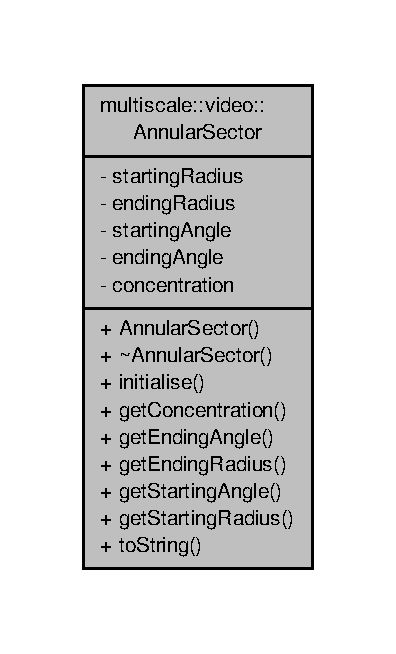
\includegraphics[width=190pt]{classmultiscale_1_1video_1_1AnnularSector__coll__graph}
\end{center}
\end{figure}
\subsection*{Public Member Functions}
\begin{DoxyCompactItemize}
\item 
\hyperlink{classmultiscale_1_1video_1_1AnnularSector_a96ea49d6d05346ef9ae99289945eb578}{Annular\-Sector} ()
\item 
\hyperlink{classmultiscale_1_1video_1_1AnnularSector_a2ced14f6af200e6e4c1c5f3e189bde4b}{$\sim$\-Annular\-Sector} ()
\item 
void \hyperlink{classmultiscale_1_1video_1_1AnnularSector_a58217c07c5c28c33f541fc37d429d79b}{initialise} (double \hyperlink{classmultiscale_1_1video_1_1AnnularSector_a4c0094d8993edb40b15580fa58a8a393}{starting\-Radius}, double \hyperlink{classmultiscale_1_1video_1_1AnnularSector_aa45c5399240707d0b3fc02ee86b97c79}{ending\-Radius}, double \hyperlink{classmultiscale_1_1video_1_1AnnularSector_a437d3dc1b2fadace28bdc3d26a78c0b3}{starting\-Angle}, double \hyperlink{classmultiscale_1_1video_1_1AnnularSector_a0aebd11072dbefe42196d6bda2e4318d}{ending\-Angle}, double \hyperlink{classmultiscale_1_1video_1_1AnnularSector_a7f6a1e7618c9e2a10e35efb5740395b1}{concentration})
\begin{DoxyCompactList}\small\item\em Initialise the members of the class. \end{DoxyCompactList}\item 
double \hyperlink{classmultiscale_1_1video_1_1AnnularSector_aee1181ae47b33a40fb2103149e45e7f1}{get\-Concentration} () const 
\begin{DoxyCompactList}\small\item\em Get the value of the concentration. \end{DoxyCompactList}\item 
double \hyperlink{classmultiscale_1_1video_1_1AnnularSector_acc074c86ca7e06ac8d5873a200498dce}{get\-Ending\-Angle} () const 
\begin{DoxyCompactList}\small\item\em Get the value of the ending angle. \end{DoxyCompactList}\item 
double \hyperlink{classmultiscale_1_1video_1_1AnnularSector_acf9600073991cf0448ab2b2997ed4513}{get\-Ending\-Radius} () const 
\begin{DoxyCompactList}\small\item\em Get the value of the ending radius. \end{DoxyCompactList}\item 
double \hyperlink{classmultiscale_1_1video_1_1AnnularSector_a85931ba16351fffc33b5a8fc714cb4b8}{get\-Starting\-Angle} () const 
\begin{DoxyCompactList}\small\item\em Get the value of the starting angle. \end{DoxyCompactList}\item 
double \hyperlink{classmultiscale_1_1video_1_1AnnularSector_aef4f23e921eae6438889f0f1537bb3ef}{get\-Starting\-Radius} () const 
\begin{DoxyCompactList}\small\item\em Get the value of the starting radius. \end{DoxyCompactList}\item 
string \hyperlink{classmultiscale_1_1video_1_1AnnularSector_ab277036c93f9dcabc08e13ca49c78e53}{to\-String} ()
\begin{DoxyCompactList}\small\item\em Get the string representation of the annular sector. \end{DoxyCompactList}\end{DoxyCompactItemize}
\subsection*{Private Attributes}
\begin{DoxyCompactItemize}
\item 
double \hyperlink{classmultiscale_1_1video_1_1AnnularSector_a4c0094d8993edb40b15580fa58a8a393}{starting\-Radius}
\item 
double \hyperlink{classmultiscale_1_1video_1_1AnnularSector_aa45c5399240707d0b3fc02ee86b97c79}{ending\-Radius}
\item 
double \hyperlink{classmultiscale_1_1video_1_1AnnularSector_a437d3dc1b2fadace28bdc3d26a78c0b3}{starting\-Angle}
\item 
double \hyperlink{classmultiscale_1_1video_1_1AnnularSector_a0aebd11072dbefe42196d6bda2e4318d}{ending\-Angle}
\item 
double \hyperlink{classmultiscale_1_1video_1_1AnnularSector_a7f6a1e7618c9e2a10e35efb5740395b1}{concentration}
\end{DoxyCompactItemize}


\subsection{Detailed Description}
An annular sector is the basic element in the considered circular geometry. 

More information about annuli and sectors of annuli can be found online (e.\-g. Wikipedia). 

Definition at line 16 of file Annular\-Sector.\-hpp.



\subsection{Constructor \& Destructor Documentation}
\hypertarget{classmultiscale_1_1video_1_1AnnularSector_a96ea49d6d05346ef9ae99289945eb578}{\index{multiscale\-::video\-::\-Annular\-Sector@{multiscale\-::video\-::\-Annular\-Sector}!Annular\-Sector@{Annular\-Sector}}
\index{Annular\-Sector@{Annular\-Sector}!multiscale::video::AnnularSector@{multiscale\-::video\-::\-Annular\-Sector}}
\subsubsection[{Annular\-Sector}]{\setlength{\rightskip}{0pt plus 5cm}Annular\-Sector\-::\-Annular\-Sector (
\begin{DoxyParamCaption}
{}
\end{DoxyParamCaption}
)}}\label{classmultiscale_1_1video_1_1AnnularSector_a96ea49d6d05346ef9ae99289945eb578}


Definition at line 11 of file Annular\-Sector.\-cpp.



References concentration, ending\-Angle, ending\-Radius, starting\-Angle, and starting\-Radius.

\hypertarget{classmultiscale_1_1video_1_1AnnularSector_a2ced14f6af200e6e4c1c5f3e189bde4b}{\index{multiscale\-::video\-::\-Annular\-Sector@{multiscale\-::video\-::\-Annular\-Sector}!$\sim$\-Annular\-Sector@{$\sim$\-Annular\-Sector}}
\index{$\sim$\-Annular\-Sector@{$\sim$\-Annular\-Sector}!multiscale::video::AnnularSector@{multiscale\-::video\-::\-Annular\-Sector}}
\subsubsection[{$\sim$\-Annular\-Sector}]{\setlength{\rightskip}{0pt plus 5cm}Annular\-Sector\-::$\sim$\-Annular\-Sector (
\begin{DoxyParamCaption}
{}
\end{DoxyParamCaption}
)}}\label{classmultiscale_1_1video_1_1AnnularSector_a2ced14f6af200e6e4c1c5f3e189bde4b}


Definition at line 19 of file Annular\-Sector.\-cpp.



\subsection{Member Function Documentation}
\hypertarget{classmultiscale_1_1video_1_1AnnularSector_aee1181ae47b33a40fb2103149e45e7f1}{\index{multiscale\-::video\-::\-Annular\-Sector@{multiscale\-::video\-::\-Annular\-Sector}!get\-Concentration@{get\-Concentration}}
\index{get\-Concentration@{get\-Concentration}!multiscale::video::AnnularSector@{multiscale\-::video\-::\-Annular\-Sector}}
\subsubsection[{get\-Concentration}]{\setlength{\rightskip}{0pt plus 5cm}double Annular\-Sector\-::get\-Concentration (
\begin{DoxyParamCaption}
{}
\end{DoxyParamCaption}
) const}}\label{classmultiscale_1_1video_1_1AnnularSector_aee1181ae47b33a40fb2103149e45e7f1}


Get the value of the concentration. 



Definition at line 30 of file Annular\-Sector.\-cpp.



References concentration.

\hypertarget{classmultiscale_1_1video_1_1AnnularSector_acc074c86ca7e06ac8d5873a200498dce}{\index{multiscale\-::video\-::\-Annular\-Sector@{multiscale\-::video\-::\-Annular\-Sector}!get\-Ending\-Angle@{get\-Ending\-Angle}}
\index{get\-Ending\-Angle@{get\-Ending\-Angle}!multiscale::video::AnnularSector@{multiscale\-::video\-::\-Annular\-Sector}}
\subsubsection[{get\-Ending\-Angle}]{\setlength{\rightskip}{0pt plus 5cm}double Annular\-Sector\-::get\-Ending\-Angle (
\begin{DoxyParamCaption}
{}
\end{DoxyParamCaption}
) const}}\label{classmultiscale_1_1video_1_1AnnularSector_acc074c86ca7e06ac8d5873a200498dce}


Get the value of the ending angle. 



Definition at line 34 of file Annular\-Sector.\-cpp.



References ending\-Angle.

\hypertarget{classmultiscale_1_1video_1_1AnnularSector_acf9600073991cf0448ab2b2997ed4513}{\index{multiscale\-::video\-::\-Annular\-Sector@{multiscale\-::video\-::\-Annular\-Sector}!get\-Ending\-Radius@{get\-Ending\-Radius}}
\index{get\-Ending\-Radius@{get\-Ending\-Radius}!multiscale::video::AnnularSector@{multiscale\-::video\-::\-Annular\-Sector}}
\subsubsection[{get\-Ending\-Radius}]{\setlength{\rightskip}{0pt plus 5cm}double Annular\-Sector\-::get\-Ending\-Radius (
\begin{DoxyParamCaption}
{}
\end{DoxyParamCaption}
) const}}\label{classmultiscale_1_1video_1_1AnnularSector_acf9600073991cf0448ab2b2997ed4513}


Get the value of the ending radius. 



Definition at line 38 of file Annular\-Sector.\-cpp.



References ending\-Radius.

\hypertarget{classmultiscale_1_1video_1_1AnnularSector_a85931ba16351fffc33b5a8fc714cb4b8}{\index{multiscale\-::video\-::\-Annular\-Sector@{multiscale\-::video\-::\-Annular\-Sector}!get\-Starting\-Angle@{get\-Starting\-Angle}}
\index{get\-Starting\-Angle@{get\-Starting\-Angle}!multiscale::video::AnnularSector@{multiscale\-::video\-::\-Annular\-Sector}}
\subsubsection[{get\-Starting\-Angle}]{\setlength{\rightskip}{0pt plus 5cm}double Annular\-Sector\-::get\-Starting\-Angle (
\begin{DoxyParamCaption}
{}
\end{DoxyParamCaption}
) const}}\label{classmultiscale_1_1video_1_1AnnularSector_a85931ba16351fffc33b5a8fc714cb4b8}


Get the value of the starting angle. 



Definition at line 42 of file Annular\-Sector.\-cpp.



References starting\-Angle.

\hypertarget{classmultiscale_1_1video_1_1AnnularSector_aef4f23e921eae6438889f0f1537bb3ef}{\index{multiscale\-::video\-::\-Annular\-Sector@{multiscale\-::video\-::\-Annular\-Sector}!get\-Starting\-Radius@{get\-Starting\-Radius}}
\index{get\-Starting\-Radius@{get\-Starting\-Radius}!multiscale::video::AnnularSector@{multiscale\-::video\-::\-Annular\-Sector}}
\subsubsection[{get\-Starting\-Radius}]{\setlength{\rightskip}{0pt plus 5cm}double Annular\-Sector\-::get\-Starting\-Radius (
\begin{DoxyParamCaption}
{}
\end{DoxyParamCaption}
) const}}\label{classmultiscale_1_1video_1_1AnnularSector_aef4f23e921eae6438889f0f1537bb3ef}


Get the value of the starting radius. 



Definition at line 46 of file Annular\-Sector.\-cpp.



References starting\-Radius.

\hypertarget{classmultiscale_1_1video_1_1AnnularSector_a58217c07c5c28c33f541fc37d429d79b}{\index{multiscale\-::video\-::\-Annular\-Sector@{multiscale\-::video\-::\-Annular\-Sector}!initialise@{initialise}}
\index{initialise@{initialise}!multiscale::video::AnnularSector@{multiscale\-::video\-::\-Annular\-Sector}}
\subsubsection[{initialise}]{\setlength{\rightskip}{0pt plus 5cm}void Annular\-Sector\-::initialise (
\begin{DoxyParamCaption}
\item[{double}]{starting\-Radius, }
\item[{double}]{ending\-Radius, }
\item[{double}]{starting\-Angle, }
\item[{double}]{ending\-Angle, }
\item[{double}]{concentration}
\end{DoxyParamCaption}
)}}\label{classmultiscale_1_1video_1_1AnnularSector_a58217c07c5c28c33f541fc37d429d79b}


Initialise the members of the class. 


\begin{DoxyParams}{Parameters}
{\em starting\-Radius} & Starting radius \\
\hline
{\em ending\-Radius} & Ending radius \\
\hline
{\em starting\-Angle} & Starting angle \\
\hline
{\em ending\-Angle} & Ending angle \\
\hline
{\em concentration} & Concentration \\
\hline
\end{DoxyParams}


Definition at line 21 of file Annular\-Sector.\-cpp.



References concentration, ending\-Angle, ending\-Radius, starting\-Angle, and starting\-Radius.

\hypertarget{classmultiscale_1_1video_1_1AnnularSector_ab277036c93f9dcabc08e13ca49c78e53}{\index{multiscale\-::video\-::\-Annular\-Sector@{multiscale\-::video\-::\-Annular\-Sector}!to\-String@{to\-String}}
\index{to\-String@{to\-String}!multiscale::video::AnnularSector@{multiscale\-::video\-::\-Annular\-Sector}}
\subsubsection[{to\-String}]{\setlength{\rightskip}{0pt plus 5cm}string Annular\-Sector\-::to\-String (
\begin{DoxyParamCaption}
{}
\end{DoxyParamCaption}
)}}\label{classmultiscale_1_1video_1_1AnnularSector_ab277036c93f9dcabc08e13ca49c78e53}


Get the string representation of the annular sector. 



Definition at line 50 of file Annular\-Sector.\-cpp.



References concentration, ending\-Angle, ending\-Radius, S\-E\-P\-A\-R\-A\-T\-O\-R, starting\-Angle, and starting\-Radius.



\subsection{Member Data Documentation}
\hypertarget{classmultiscale_1_1video_1_1AnnularSector_a7f6a1e7618c9e2a10e35efb5740395b1}{\index{multiscale\-::video\-::\-Annular\-Sector@{multiscale\-::video\-::\-Annular\-Sector}!concentration@{concentration}}
\index{concentration@{concentration}!multiscale::video::AnnularSector@{multiscale\-::video\-::\-Annular\-Sector}}
\subsubsection[{concentration}]{\setlength{\rightskip}{0pt plus 5cm}double multiscale\-::video\-::\-Annular\-Sector\-::concentration\hspace{0.3cm}{\ttfamily [private]}}}\label{classmultiscale_1_1video_1_1AnnularSector_a7f6a1e7618c9e2a10e35efb5740395b1}


Definition at line 24 of file Annular\-Sector.\-hpp.



Referenced by Annular\-Sector(), get\-Concentration(), initialise(), and to\-String().

\hypertarget{classmultiscale_1_1video_1_1AnnularSector_a0aebd11072dbefe42196d6bda2e4318d}{\index{multiscale\-::video\-::\-Annular\-Sector@{multiscale\-::video\-::\-Annular\-Sector}!ending\-Angle@{ending\-Angle}}
\index{ending\-Angle@{ending\-Angle}!multiscale::video::AnnularSector@{multiscale\-::video\-::\-Annular\-Sector}}
\subsubsection[{ending\-Angle}]{\setlength{\rightskip}{0pt plus 5cm}double multiscale\-::video\-::\-Annular\-Sector\-::ending\-Angle\hspace{0.3cm}{\ttfamily [private]}}}\label{classmultiscale_1_1video_1_1AnnularSector_a0aebd11072dbefe42196d6bda2e4318d}


Definition at line 23 of file Annular\-Sector.\-hpp.



Referenced by Annular\-Sector(), get\-Ending\-Angle(), initialise(), and to\-String().

\hypertarget{classmultiscale_1_1video_1_1AnnularSector_aa45c5399240707d0b3fc02ee86b97c79}{\index{multiscale\-::video\-::\-Annular\-Sector@{multiscale\-::video\-::\-Annular\-Sector}!ending\-Radius@{ending\-Radius}}
\index{ending\-Radius@{ending\-Radius}!multiscale::video::AnnularSector@{multiscale\-::video\-::\-Annular\-Sector}}
\subsubsection[{ending\-Radius}]{\setlength{\rightskip}{0pt plus 5cm}double multiscale\-::video\-::\-Annular\-Sector\-::ending\-Radius\hspace{0.3cm}{\ttfamily [private]}}}\label{classmultiscale_1_1video_1_1AnnularSector_aa45c5399240707d0b3fc02ee86b97c79}


Definition at line 21 of file Annular\-Sector.\-hpp.



Referenced by Annular\-Sector(), get\-Ending\-Radius(), initialise(), and to\-String().

\hypertarget{classmultiscale_1_1video_1_1AnnularSector_a437d3dc1b2fadace28bdc3d26a78c0b3}{\index{multiscale\-::video\-::\-Annular\-Sector@{multiscale\-::video\-::\-Annular\-Sector}!starting\-Angle@{starting\-Angle}}
\index{starting\-Angle@{starting\-Angle}!multiscale::video::AnnularSector@{multiscale\-::video\-::\-Annular\-Sector}}
\subsubsection[{starting\-Angle}]{\setlength{\rightskip}{0pt plus 5cm}double multiscale\-::video\-::\-Annular\-Sector\-::starting\-Angle\hspace{0.3cm}{\ttfamily [private]}}}\label{classmultiscale_1_1video_1_1AnnularSector_a437d3dc1b2fadace28bdc3d26a78c0b3}


Definition at line 22 of file Annular\-Sector.\-hpp.



Referenced by Annular\-Sector(), get\-Starting\-Angle(), initialise(), and to\-String().

\hypertarget{classmultiscale_1_1video_1_1AnnularSector_a4c0094d8993edb40b15580fa58a8a393}{\index{multiscale\-::video\-::\-Annular\-Sector@{multiscale\-::video\-::\-Annular\-Sector}!starting\-Radius@{starting\-Radius}}
\index{starting\-Radius@{starting\-Radius}!multiscale::video::AnnularSector@{multiscale\-::video\-::\-Annular\-Sector}}
\subsubsection[{starting\-Radius}]{\setlength{\rightskip}{0pt plus 5cm}double multiscale\-::video\-::\-Annular\-Sector\-::starting\-Radius\hspace{0.3cm}{\ttfamily [private]}}}\label{classmultiscale_1_1video_1_1AnnularSector_a4c0094d8993edb40b15580fa58a8a393}


Definition at line 20 of file Annular\-Sector.\-hpp.



Referenced by Annular\-Sector(), get\-Starting\-Radius(), initialise(), and to\-String().



The documentation for this class was generated from the following files\-:\begin{DoxyCompactItemize}
\item 
/home/ovidiu/\-Repositories/git/multiscale/\-Multiscale/modules/video/circular/include/multiscale/video/circular/\hyperlink{AnnularSector_8hpp}{Annular\-Sector.\-hpp}\item 
/home/ovidiu/\-Repositories/git/multiscale/\-Multiscale/modules/video/circular/src/\hyperlink{AnnularSector_8cpp}{Annular\-Sector.\-cpp}\end{DoxyCompactItemize}

\hypertarget{classmultiscale_1_1video_1_1CartesianToConcentrationsConverter}{\section{multiscale\-:\-:video\-:\-:Cartesian\-To\-Concentrations\-Converter Class Reference}
\label{classmultiscale_1_1video_1_1CartesianToConcentrationsConverter}\index{multiscale\-::video\-::\-Cartesian\-To\-Concentrations\-Converter@{multiscale\-::video\-::\-Cartesian\-To\-Concentrations\-Converter}}
}


Scale the values of the rectangular geometry grid cells.  




{\ttfamily \#include $<$Cartesian\-To\-Concentrations\-Converter.\-hpp$>$}



Collaboration diagram for multiscale\-:\-:video\-:\-:Cartesian\-To\-Concentrations\-Converter\-:\nopagebreak
\begin{figure}[H]
\begin{center}
\leavevmode
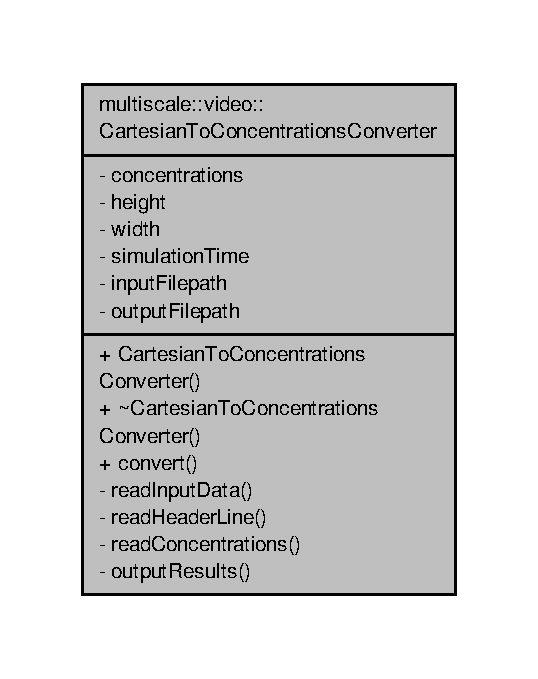
\includegraphics[width=258pt]{classmultiscale_1_1video_1_1CartesianToConcentrationsConverter__coll__graph}
\end{center}
\end{figure}
\subsection*{Public Member Functions}
\begin{DoxyCompactItemize}
\item 
\hyperlink{classmultiscale_1_1video_1_1CartesianToConcentrationsConverter_ae2f641fe6c2af730a5aedc83f4bc1244}{Cartesian\-To\-Concentrations\-Converter} (const string \&\hyperlink{classmultiscale_1_1video_1_1CartesianToConcentrationsConverter_affebbc7e1c67692bd529f19fc0451e58}{input\-Filepath}, const string \&\hyperlink{classmultiscale_1_1video_1_1CartesianToConcentrationsConverter_a9215448e33876a581b206a89b6651fd0}{output\-Filepath})
\item 
\hyperlink{classmultiscale_1_1video_1_1CartesianToConcentrationsConverter_a4250cb00af6f3c254c0577479ae25553}{$\sim$\-Cartesian\-To\-Concentrations\-Converter} ()
\item 
void \hyperlink{classmultiscale_1_1video_1_1CartesianToConcentrationsConverter_a27de97c7e35097bd17453fd07f33a6f1}{convert} ()
\begin{DoxyCompactList}\small\item\em Start the conversion. \end{DoxyCompactList}\end{DoxyCompactItemize}
\subsection*{Private Member Functions}
\begin{DoxyCompactItemize}
\item 
void \hyperlink{classmultiscale_1_1video_1_1CartesianToConcentrationsConverter_a94094cdeaf0f48164911188709dc0e2f}{read\-Input\-Data} ()
\begin{DoxyCompactList}\small\item\em Read the input data. \end{DoxyCompactList}\item 
void \hyperlink{classmultiscale_1_1video_1_1CartesianToConcentrationsConverter_a2e9967ae6fb2efc39ed377aca2fa222c}{read\-Header\-Line} (ifstream \&fin)
\begin{DoxyCompactList}\small\item\em Read the header line. \end{DoxyCompactList}\item 
void \hyperlink{classmultiscale_1_1video_1_1CartesianToConcentrationsConverter_a9134409b814fafe62c896c6b473bc574}{read\-Concentrations} (ifstream \&fin)
\begin{DoxyCompactList}\small\item\em Read the concentrations. \end{DoxyCompactList}\item 
void \hyperlink{classmultiscale_1_1video_1_1CartesianToConcentrationsConverter_a346e054266585ae6922d159b8d5fb804}{output\-Results} ()
\begin{DoxyCompactList}\small\item\em Output the results. \end{DoxyCompactList}\end{DoxyCompactItemize}
\subsection*{Private Attributes}
\begin{DoxyCompactItemize}
\item 
vector$<$ double $>$ \hyperlink{classmultiscale_1_1video_1_1CartesianToConcentrationsConverter_a335f54163cbabeaa80c1da811b9f9c0c}{concentrations}
\item 
unsigned long \hyperlink{classmultiscale_1_1video_1_1CartesianToConcentrationsConverter_a94e58072f2e143bd6476133370ffb37f}{height}
\item 
unsigned long \hyperlink{classmultiscale_1_1video_1_1CartesianToConcentrationsConverter_ae6fba5af405d884c7b70ed206a6d5cb1}{width}
\item 
double \hyperlink{classmultiscale_1_1video_1_1CartesianToConcentrationsConverter_a6e66af60b82513b3186fdb32cad44597}{simulation\-Time}
\item 
string \hyperlink{classmultiscale_1_1video_1_1CartesianToConcentrationsConverter_affebbc7e1c67692bd529f19fc0451e58}{input\-Filepath}
\item 
string \hyperlink{classmultiscale_1_1video_1_1CartesianToConcentrationsConverter_a9215448e33876a581b206a89b6651fd0}{output\-Filepath}
\end{DoxyCompactItemize}


\subsection{Detailed Description}
Scale the values of the rectangular geometry grid cells. 

Definition at line 26 of file Cartesian\-To\-Concentrations\-Converter.\-hpp.



\subsection{Constructor \& Destructor Documentation}
\hypertarget{classmultiscale_1_1video_1_1CartesianToConcentrationsConverter_ae2f641fe6c2af730a5aedc83f4bc1244}{\index{multiscale\-::video\-::\-Cartesian\-To\-Concentrations\-Converter@{multiscale\-::video\-::\-Cartesian\-To\-Concentrations\-Converter}!Cartesian\-To\-Concentrations\-Converter@{Cartesian\-To\-Concentrations\-Converter}}
\index{Cartesian\-To\-Concentrations\-Converter@{Cartesian\-To\-Concentrations\-Converter}!multiscale::video::CartesianToConcentrationsConverter@{multiscale\-::video\-::\-Cartesian\-To\-Concentrations\-Converter}}
\subsubsection[{Cartesian\-To\-Concentrations\-Converter}]{\setlength{\rightskip}{0pt plus 5cm}Cartesian\-To\-Concentrations\-Converter\-::\-Cartesian\-To\-Concentrations\-Converter (
\begin{DoxyParamCaption}
\item[{const string \&}]{input\-Filepath, }
\item[{const string \&}]{output\-Filepath}
\end{DoxyParamCaption}
)}}\label{classmultiscale_1_1video_1_1CartesianToConcentrationsConverter_ae2f641fe6c2af730a5aedc83f4bc1244}


Definition at line 15 of file Cartesian\-To\-Concentrations\-Converter.\-cpp.



References height, simulation\-Time, and width.

\hypertarget{classmultiscale_1_1video_1_1CartesianToConcentrationsConverter_a4250cb00af6f3c254c0577479ae25553}{\index{multiscale\-::video\-::\-Cartesian\-To\-Concentrations\-Converter@{multiscale\-::video\-::\-Cartesian\-To\-Concentrations\-Converter}!$\sim$\-Cartesian\-To\-Concentrations\-Converter@{$\sim$\-Cartesian\-To\-Concentrations\-Converter}}
\index{$\sim$\-Cartesian\-To\-Concentrations\-Converter@{$\sim$\-Cartesian\-To\-Concentrations\-Converter}!multiscale::video::CartesianToConcentrationsConverter@{multiscale\-::video\-::\-Cartesian\-To\-Concentrations\-Converter}}
\subsubsection[{$\sim$\-Cartesian\-To\-Concentrations\-Converter}]{\setlength{\rightskip}{0pt plus 5cm}Cartesian\-To\-Concentrations\-Converter\-::$\sim$\-Cartesian\-To\-Concentrations\-Converter (
\begin{DoxyParamCaption}
{}
\end{DoxyParamCaption}
)}}\label{classmultiscale_1_1video_1_1CartesianToConcentrationsConverter_a4250cb00af6f3c254c0577479ae25553}


Definition at line 24 of file Cartesian\-To\-Concentrations\-Converter.\-cpp.



\subsection{Member Function Documentation}
\hypertarget{classmultiscale_1_1video_1_1CartesianToConcentrationsConverter_a27de97c7e35097bd17453fd07f33a6f1}{\index{multiscale\-::video\-::\-Cartesian\-To\-Concentrations\-Converter@{multiscale\-::video\-::\-Cartesian\-To\-Concentrations\-Converter}!convert@{convert}}
\index{convert@{convert}!multiscale::video::CartesianToConcentrationsConverter@{multiscale\-::video\-::\-Cartesian\-To\-Concentrations\-Converter}}
\subsubsection[{convert}]{\setlength{\rightskip}{0pt plus 5cm}void Cartesian\-To\-Concentrations\-Converter\-::convert (
\begin{DoxyParamCaption}
{}
\end{DoxyParamCaption}
)}}\label{classmultiscale_1_1video_1_1CartesianToConcentrationsConverter_a27de97c7e35097bd17453fd07f33a6f1}


Start the conversion. 



Definition at line 26 of file Cartesian\-To\-Concentrations\-Converter.\-cpp.



References output\-Results(), and read\-Input\-Data().



Referenced by main().



Here is the call graph for this function\-:\nopagebreak
\begin{figure}[H]
\begin{center}
\leavevmode
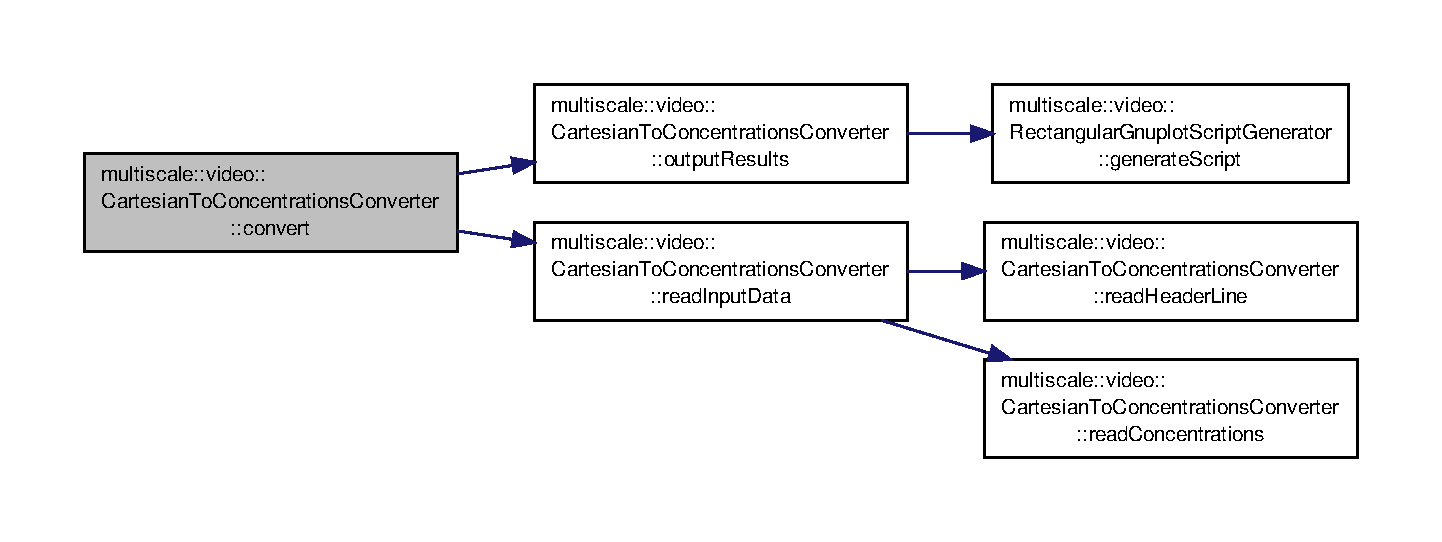
\includegraphics[width=350pt]{classmultiscale_1_1video_1_1CartesianToConcentrationsConverter_a27de97c7e35097bd17453fd07f33a6f1_cgraph}
\end{center}
\end{figure}




Here is the caller graph for this function\-:\nopagebreak
\begin{figure}[H]
\begin{center}
\leavevmode
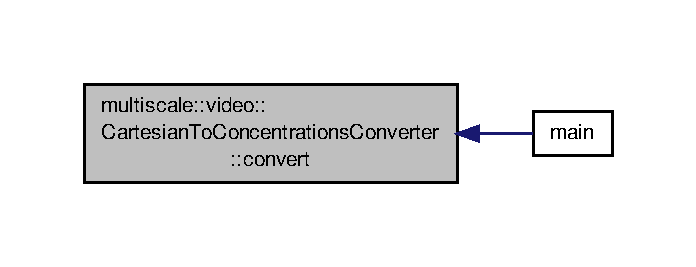
\includegraphics[width=334pt]{classmultiscale_1_1video_1_1CartesianToConcentrationsConverter_a27de97c7e35097bd17453fd07f33a6f1_icgraph}
\end{center}
\end{figure}


\hypertarget{classmultiscale_1_1video_1_1CartesianToConcentrationsConverter_a346e054266585ae6922d159b8d5fb804}{\index{multiscale\-::video\-::\-Cartesian\-To\-Concentrations\-Converter@{multiscale\-::video\-::\-Cartesian\-To\-Concentrations\-Converter}!output\-Results@{output\-Results}}
\index{output\-Results@{output\-Results}!multiscale::video::CartesianToConcentrationsConverter@{multiscale\-::video\-::\-Cartesian\-To\-Concentrations\-Converter}}
\subsubsection[{output\-Results}]{\setlength{\rightskip}{0pt plus 5cm}void Cartesian\-To\-Concentrations\-Converter\-::output\-Results (
\begin{DoxyParamCaption}
{}
\end{DoxyParamCaption}
)\hspace{0.3cm}{\ttfamily [private]}}}\label{classmultiscale_1_1video_1_1CartesianToConcentrationsConverter_a346e054266585ae6922d159b8d5fb804}


Output the results. 



Definition at line 84 of file Cartesian\-To\-Concentrations\-Converter.\-cpp.



References concentrations, multiscale\-::video\-::\-Rectangular\-Gnuplot\-Script\-Generator\-::generate\-Script(), height, output\-Filepath, simulation\-Time, and width.



Referenced by convert().



Here is the call graph for this function\-:\nopagebreak
\begin{figure}[H]
\begin{center}
\leavevmode
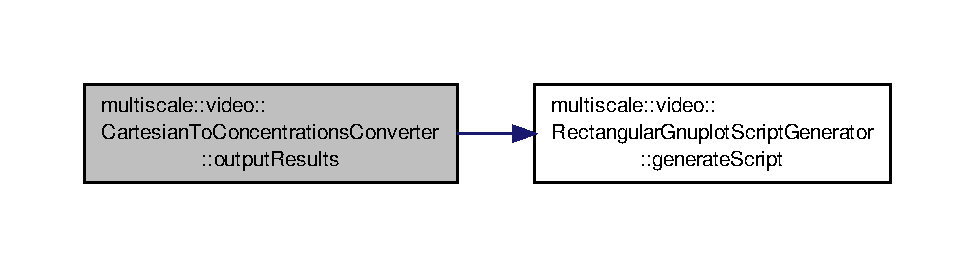
\includegraphics[width=350pt]{classmultiscale_1_1video_1_1CartesianToConcentrationsConverter_a346e054266585ae6922d159b8d5fb804_cgraph}
\end{center}
\end{figure}




Here is the caller graph for this function\-:\nopagebreak
\begin{figure}[H]
\begin{center}
\leavevmode
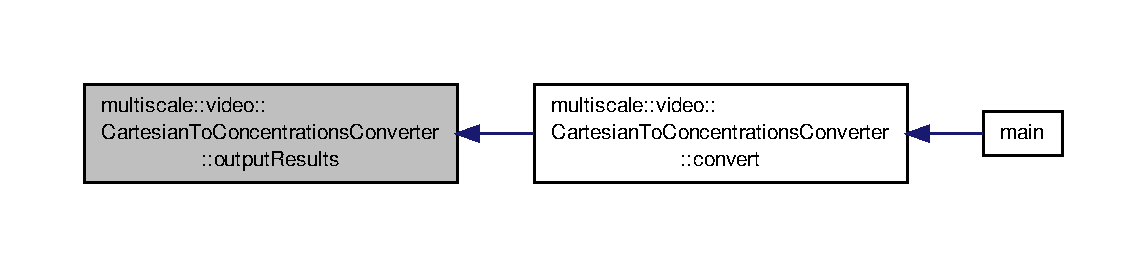
\includegraphics[width=350pt]{classmultiscale_1_1video_1_1CartesianToConcentrationsConverter_a346e054266585ae6922d159b8d5fb804_icgraph}
\end{center}
\end{figure}


\hypertarget{classmultiscale_1_1video_1_1CartesianToConcentrationsConverter_a9134409b814fafe62c896c6b473bc574}{\index{multiscale\-::video\-::\-Cartesian\-To\-Concentrations\-Converter@{multiscale\-::video\-::\-Cartesian\-To\-Concentrations\-Converter}!read\-Concentrations@{read\-Concentrations}}
\index{read\-Concentrations@{read\-Concentrations}!multiscale::video::CartesianToConcentrationsConverter@{multiscale\-::video\-::\-Cartesian\-To\-Concentrations\-Converter}}
\subsubsection[{read\-Concentrations}]{\setlength{\rightskip}{0pt plus 5cm}void Cartesian\-To\-Concentrations\-Converter\-::read\-Concentrations (
\begin{DoxyParamCaption}
\item[{ifstream \&}]{fin}
\end{DoxyParamCaption}
)\hspace{0.3cm}{\ttfamily [private]}}}\label{classmultiscale_1_1video_1_1CartesianToConcentrationsConverter_a9134409b814fafe62c896c6b473bc574}


Read the concentrations. 


\begin{DoxyParams}{Parameters}
{\em fin} & Input file stream \\
\hline
\end{DoxyParams}


Definition at line 64 of file Cartesian\-To\-Concentrations\-Converter.\-cpp.



References concentrations, E\-R\-R\-\_\-\-C\-O\-N\-C, height, and width.



Referenced by read\-Input\-Data().



Here is the caller graph for this function\-:\nopagebreak
\begin{figure}[H]
\begin{center}
\leavevmode
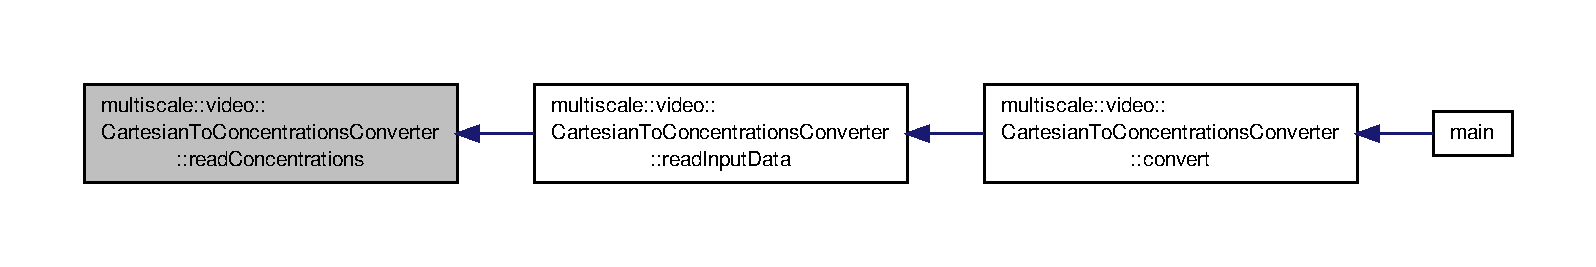
\includegraphics[width=350pt]{classmultiscale_1_1video_1_1CartesianToConcentrationsConverter_a9134409b814fafe62c896c6b473bc574_icgraph}
\end{center}
\end{figure}


\hypertarget{classmultiscale_1_1video_1_1CartesianToConcentrationsConverter_a2e9967ae6fb2efc39ed377aca2fa222c}{\index{multiscale\-::video\-::\-Cartesian\-To\-Concentrations\-Converter@{multiscale\-::video\-::\-Cartesian\-To\-Concentrations\-Converter}!read\-Header\-Line@{read\-Header\-Line}}
\index{read\-Header\-Line@{read\-Header\-Line}!multiscale::video::CartesianToConcentrationsConverter@{multiscale\-::video\-::\-Cartesian\-To\-Concentrations\-Converter}}
\subsubsection[{read\-Header\-Line}]{\setlength{\rightskip}{0pt plus 5cm}void Cartesian\-To\-Concentrations\-Converter\-::read\-Header\-Line (
\begin{DoxyParamCaption}
\item[{ifstream \&}]{fin}
\end{DoxyParamCaption}
)\hspace{0.3cm}{\ttfamily [private]}}}\label{classmultiscale_1_1video_1_1CartesianToConcentrationsConverter_a2e9967ae6fb2efc39ed377aca2fa222c}


Read the header line. 

The header line contains values for number of concentric circles, number of sectors and simulation time


\begin{DoxyParams}{Parameters}
{\em fin} & Input file stream \\
\hline
\end{DoxyParams}


Definition at line 55 of file Cartesian\-To\-Concentrations\-Converter.\-cpp.



References E\-R\-R\-\_\-\-N\-E\-G\-\_\-\-S\-I\-M\-\_\-\-T\-I\-M\-E, E\-R\-R\-\_\-\-N\-O\-N\-P\-O\-S\-\_\-\-D\-I\-M\-E\-N\-S\-I\-O\-N, height, simulation\-Time, and width.



Referenced by read\-Input\-Data().



Here is the caller graph for this function\-:\nopagebreak
\begin{figure}[H]
\begin{center}
\leavevmode
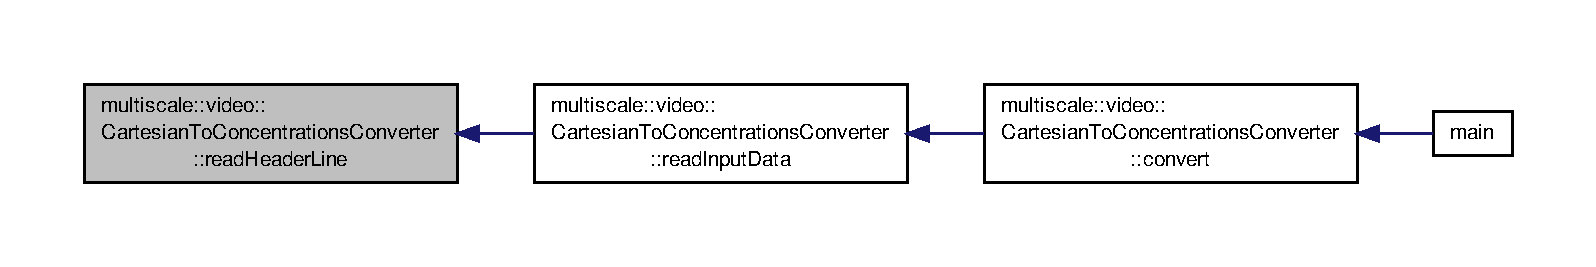
\includegraphics[width=350pt]{classmultiscale_1_1video_1_1CartesianToConcentrationsConverter_a2e9967ae6fb2efc39ed377aca2fa222c_icgraph}
\end{center}
\end{figure}


\hypertarget{classmultiscale_1_1video_1_1CartesianToConcentrationsConverter_a94094cdeaf0f48164911188709dc0e2f}{\index{multiscale\-::video\-::\-Cartesian\-To\-Concentrations\-Converter@{multiscale\-::video\-::\-Cartesian\-To\-Concentrations\-Converter}!read\-Input\-Data@{read\-Input\-Data}}
\index{read\-Input\-Data@{read\-Input\-Data}!multiscale::video::CartesianToConcentrationsConverter@{multiscale\-::video\-::\-Cartesian\-To\-Concentrations\-Converter}}
\subsubsection[{read\-Input\-Data}]{\setlength{\rightskip}{0pt plus 5cm}void Cartesian\-To\-Concentrations\-Converter\-::read\-Input\-Data (
\begin{DoxyParamCaption}
{}
\end{DoxyParamCaption}
)\hspace{0.3cm}{\ttfamily [private]}}}\label{classmultiscale_1_1video_1_1CartesianToConcentrationsConverter_a94094cdeaf0f48164911188709dc0e2f}


Read the input data. 



Definition at line 31 of file Cartesian\-To\-Concentrations\-Converter.\-cpp.



References E\-R\-R\-\_\-\-I\-N\-\_\-\-E\-X\-T\-R\-A\-\_\-\-D\-A\-T\-A, E\-R\-R\-\_\-\-I\-N\-P\-U\-T\-\_\-\-O\-P\-E\-N, input\-Filepath, read\-Concentrations(), and read\-Header\-Line().



Referenced by convert().



Here is the call graph for this function\-:\nopagebreak
\begin{figure}[H]
\begin{center}
\leavevmode
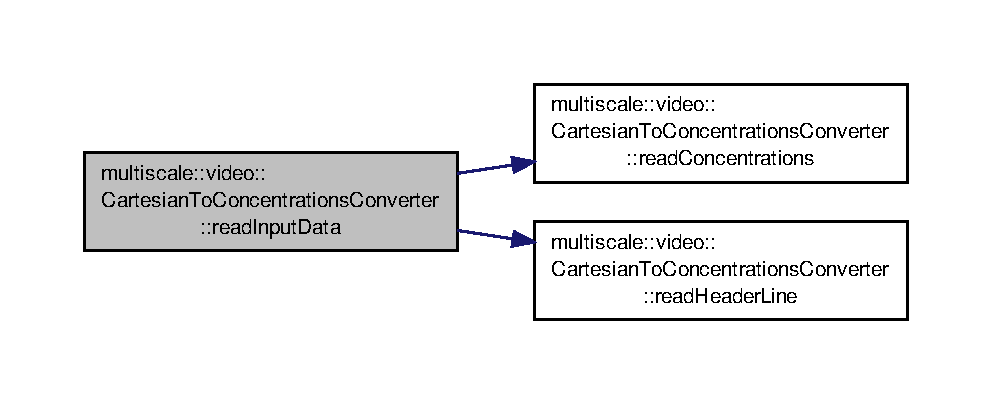
\includegraphics[width=350pt]{classmultiscale_1_1video_1_1CartesianToConcentrationsConverter_a94094cdeaf0f48164911188709dc0e2f_cgraph}
\end{center}
\end{figure}




Here is the caller graph for this function\-:\nopagebreak
\begin{figure}[H]
\begin{center}
\leavevmode
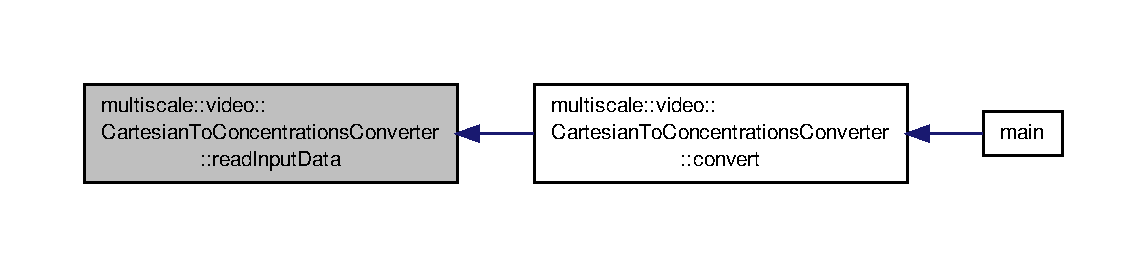
\includegraphics[width=350pt]{classmultiscale_1_1video_1_1CartesianToConcentrationsConverter_a94094cdeaf0f48164911188709dc0e2f_icgraph}
\end{center}
\end{figure}




\subsection{Member Data Documentation}
\hypertarget{classmultiscale_1_1video_1_1CartesianToConcentrationsConverter_a335f54163cbabeaa80c1da811b9f9c0c}{\index{multiscale\-::video\-::\-Cartesian\-To\-Concentrations\-Converter@{multiscale\-::video\-::\-Cartesian\-To\-Concentrations\-Converter}!concentrations@{concentrations}}
\index{concentrations@{concentrations}!multiscale::video::CartesianToConcentrationsConverter@{multiscale\-::video\-::\-Cartesian\-To\-Concentrations\-Converter}}
\subsubsection[{concentrations}]{\setlength{\rightskip}{0pt plus 5cm}vector$<$double$>$ multiscale\-::video\-::\-Cartesian\-To\-Concentrations\-Converter\-::concentrations\hspace{0.3cm}{\ttfamily [private]}}}\label{classmultiscale_1_1video_1_1CartesianToConcentrationsConverter_a335f54163cbabeaa80c1da811b9f9c0c}
Concentrations received as input 

Definition at line 30 of file Cartesian\-To\-Concentrations\-Converter.\-hpp.



Referenced by output\-Results(), and read\-Concentrations().

\hypertarget{classmultiscale_1_1video_1_1CartesianToConcentrationsConverter_a94e58072f2e143bd6476133370ffb37f}{\index{multiscale\-::video\-::\-Cartesian\-To\-Concentrations\-Converter@{multiscale\-::video\-::\-Cartesian\-To\-Concentrations\-Converter}!height@{height}}
\index{height@{height}!multiscale::video::CartesianToConcentrationsConverter@{multiscale\-::video\-::\-Cartesian\-To\-Concentrations\-Converter}}
\subsubsection[{height}]{\setlength{\rightskip}{0pt plus 5cm}unsigned long multiscale\-::video\-::\-Cartesian\-To\-Concentrations\-Converter\-::height\hspace{0.3cm}{\ttfamily [private]}}}\label{classmultiscale_1_1video_1_1CartesianToConcentrationsConverter_a94e58072f2e143bd6476133370ffb37f}
Height of the grid 

Definition at line 32 of file Cartesian\-To\-Concentrations\-Converter.\-hpp.



Referenced by Cartesian\-To\-Concentrations\-Converter(), output\-Results(), read\-Concentrations(), and read\-Header\-Line().

\hypertarget{classmultiscale_1_1video_1_1CartesianToConcentrationsConverter_affebbc7e1c67692bd529f19fc0451e58}{\index{multiscale\-::video\-::\-Cartesian\-To\-Concentrations\-Converter@{multiscale\-::video\-::\-Cartesian\-To\-Concentrations\-Converter}!input\-Filepath@{input\-Filepath}}
\index{input\-Filepath@{input\-Filepath}!multiscale::video::CartesianToConcentrationsConverter@{multiscale\-::video\-::\-Cartesian\-To\-Concentrations\-Converter}}
\subsubsection[{input\-Filepath}]{\setlength{\rightskip}{0pt plus 5cm}string multiscale\-::video\-::\-Cartesian\-To\-Concentrations\-Converter\-::input\-Filepath\hspace{0.3cm}{\ttfamily [private]}}}\label{classmultiscale_1_1video_1_1CartesianToConcentrationsConverter_affebbc7e1c67692bd529f19fc0451e58}
Path to the input file 

Definition at line 36 of file Cartesian\-To\-Concentrations\-Converter.\-hpp.



Referenced by read\-Input\-Data().

\hypertarget{classmultiscale_1_1video_1_1CartesianToConcentrationsConverter_a9215448e33876a581b206a89b6651fd0}{\index{multiscale\-::video\-::\-Cartesian\-To\-Concentrations\-Converter@{multiscale\-::video\-::\-Cartesian\-To\-Concentrations\-Converter}!output\-Filepath@{output\-Filepath}}
\index{output\-Filepath@{output\-Filepath}!multiscale::video::CartesianToConcentrationsConverter@{multiscale\-::video\-::\-Cartesian\-To\-Concentrations\-Converter}}
\subsubsection[{output\-Filepath}]{\setlength{\rightskip}{0pt plus 5cm}string multiscale\-::video\-::\-Cartesian\-To\-Concentrations\-Converter\-::output\-Filepath\hspace{0.3cm}{\ttfamily [private]}}}\label{classmultiscale_1_1video_1_1CartesianToConcentrationsConverter_a9215448e33876a581b206a89b6651fd0}
Path to the output file 

Definition at line 37 of file Cartesian\-To\-Concentrations\-Converter.\-hpp.



Referenced by output\-Results().

\hypertarget{classmultiscale_1_1video_1_1CartesianToConcentrationsConverter_a6e66af60b82513b3186fdb32cad44597}{\index{multiscale\-::video\-::\-Cartesian\-To\-Concentrations\-Converter@{multiscale\-::video\-::\-Cartesian\-To\-Concentrations\-Converter}!simulation\-Time@{simulation\-Time}}
\index{simulation\-Time@{simulation\-Time}!multiscale::video::CartesianToConcentrationsConverter@{multiscale\-::video\-::\-Cartesian\-To\-Concentrations\-Converter}}
\subsubsection[{simulation\-Time}]{\setlength{\rightskip}{0pt plus 5cm}double multiscale\-::video\-::\-Cartesian\-To\-Concentrations\-Converter\-::simulation\-Time\hspace{0.3cm}{\ttfamily [private]}}}\label{classmultiscale_1_1video_1_1CartesianToConcentrationsConverter_a6e66af60b82513b3186fdb32cad44597}
Simulation time 

Definition at line 34 of file Cartesian\-To\-Concentrations\-Converter.\-hpp.



Referenced by Cartesian\-To\-Concentrations\-Converter(), output\-Results(), and read\-Header\-Line().

\hypertarget{classmultiscale_1_1video_1_1CartesianToConcentrationsConverter_ae6fba5af405d884c7b70ed206a6d5cb1}{\index{multiscale\-::video\-::\-Cartesian\-To\-Concentrations\-Converter@{multiscale\-::video\-::\-Cartesian\-To\-Concentrations\-Converter}!width@{width}}
\index{width@{width}!multiscale::video::CartesianToConcentrationsConverter@{multiscale\-::video\-::\-Cartesian\-To\-Concentrations\-Converter}}
\subsubsection[{width}]{\setlength{\rightskip}{0pt plus 5cm}unsigned long multiscale\-::video\-::\-Cartesian\-To\-Concentrations\-Converter\-::width\hspace{0.3cm}{\ttfamily [private]}}}\label{classmultiscale_1_1video_1_1CartesianToConcentrationsConverter_ae6fba5af405d884c7b70ed206a6d5cb1}
Width of the grid 

Definition at line 33 of file Cartesian\-To\-Concentrations\-Converter.\-hpp.



Referenced by Cartesian\-To\-Concentrations\-Converter(), output\-Results(), read\-Concentrations(), and read\-Header\-Line().



The documentation for this class was generated from the following files\-:\begin{DoxyCompactItemize}
\item 
include/multiscale/video/rectangular/\hyperlink{CartesianToConcentrationsConverter_8hpp}{Cartesian\-To\-Concentrations\-Converter.\-hpp}\item 
src/multiscale/video/rectangular/\hyperlink{CartesianToConcentrationsConverter_8cpp}{Cartesian\-To\-Concentrations\-Converter.\-cpp}\end{DoxyCompactItemize}

\hypertarget{classmultiscale_1_1CartesianToConcentrationsConverterException}{\section{multiscale\-:\-:Cartesian\-To\-Concentrations\-Converter\-Exception Class Reference}
\label{classmultiscale_1_1CartesianToConcentrationsConverterException}\index{multiscale\-::\-Cartesian\-To\-Concentrations\-Converter\-Exception@{multiscale\-::\-Cartesian\-To\-Concentrations\-Converter\-Exception}}
}


Exception class for the Cartesian\-To\-Concentrations\-Converter class.  




{\ttfamily \#include $<$Cartesian\-To\-Concentrations\-Converter\-Exception.\-hpp$>$}



Inheritance diagram for multiscale\-:\-:Cartesian\-To\-Concentrations\-Converter\-Exception\-:\nopagebreak
\begin{figure}[H]
\begin{center}
\leavevmode
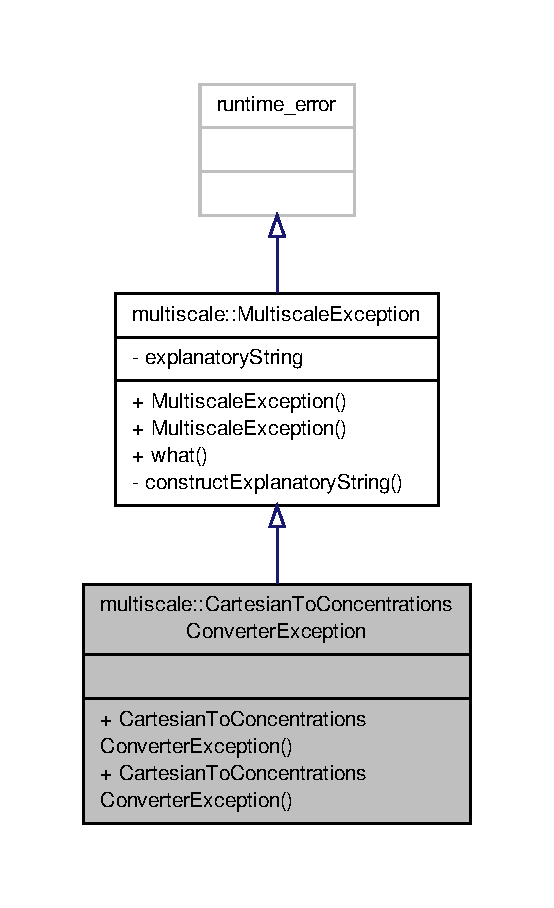
\includegraphics[width=266pt]{classmultiscale_1_1CartesianToConcentrationsConverterException__inherit__graph}
\end{center}
\end{figure}


Collaboration diagram for multiscale\-:\-:Cartesian\-To\-Concentrations\-Converter\-Exception\-:\nopagebreak
\begin{figure}[H]
\begin{center}
\leavevmode
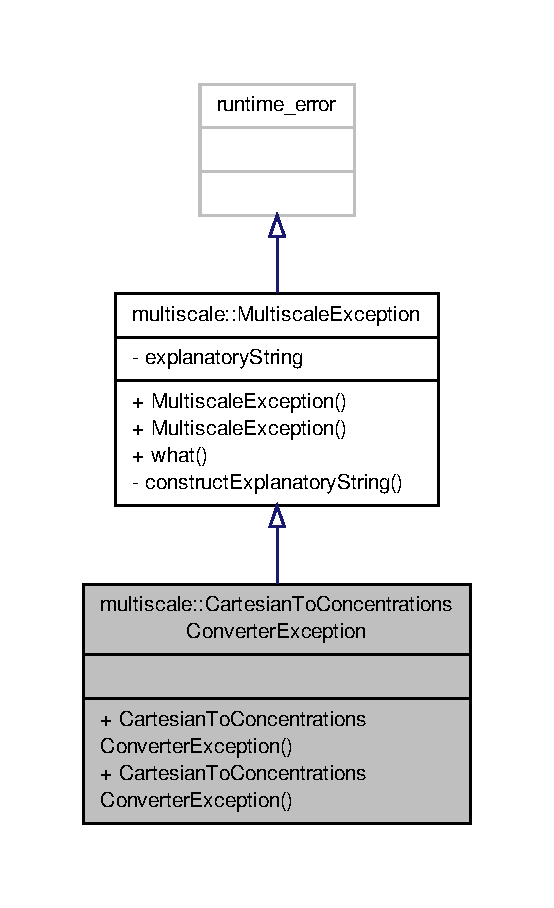
\includegraphics[width=266pt]{classmultiscale_1_1CartesianToConcentrationsConverterException__coll__graph}
\end{center}
\end{figure}
\subsection*{Public Member Functions}
\begin{DoxyCompactItemize}
\item 
\hyperlink{classmultiscale_1_1CartesianToConcentrationsConverterException_aa5f13cfa28fc44eda6bc2c53382e6749}{Cartesian\-To\-Concentrations\-Converter\-Exception} (const string \&msg)
\item 
\hyperlink{classmultiscale_1_1CartesianToConcentrationsConverterException_a91a1cee8ddfefb30eb0d01ff2afbd3e7}{Cartesian\-To\-Concentrations\-Converter\-Exception} (const char $\ast$msg)
\end{DoxyCompactItemize}


\subsection{Detailed Description}
Exception class for the Cartesian\-To\-Concentrations\-Converter class. 

Definition at line 13 of file Cartesian\-To\-Concentrations\-Converter\-Exception.\-hpp.



\subsection{Constructor \& Destructor Documentation}
\hypertarget{classmultiscale_1_1CartesianToConcentrationsConverterException_aa5f13cfa28fc44eda6bc2c53382e6749}{\index{multiscale\-::\-Cartesian\-To\-Concentrations\-Converter\-Exception@{multiscale\-::\-Cartesian\-To\-Concentrations\-Converter\-Exception}!Cartesian\-To\-Concentrations\-Converter\-Exception@{Cartesian\-To\-Concentrations\-Converter\-Exception}}
\index{Cartesian\-To\-Concentrations\-Converter\-Exception@{Cartesian\-To\-Concentrations\-Converter\-Exception}!multiscale::CartesianToConcentrationsConverterException@{multiscale\-::\-Cartesian\-To\-Concentrations\-Converter\-Exception}}
\subsubsection[{Cartesian\-To\-Concentrations\-Converter\-Exception}]{\setlength{\rightskip}{0pt plus 5cm}multiscale\-::\-Cartesian\-To\-Concentrations\-Converter\-Exception\-::\-Cartesian\-To\-Concentrations\-Converter\-Exception (
\begin{DoxyParamCaption}
\item[{const string \&}]{msg}
\end{DoxyParamCaption}
)\hspace{0.3cm}{\ttfamily [inline]}}}\label{classmultiscale_1_1CartesianToConcentrationsConverterException_aa5f13cfa28fc44eda6bc2c53382e6749}


Definition at line 17 of file Cartesian\-To\-Concentrations\-Converter\-Exception.\-hpp.

\hypertarget{classmultiscale_1_1CartesianToConcentrationsConverterException_a91a1cee8ddfefb30eb0d01ff2afbd3e7}{\index{multiscale\-::\-Cartesian\-To\-Concentrations\-Converter\-Exception@{multiscale\-::\-Cartesian\-To\-Concentrations\-Converter\-Exception}!Cartesian\-To\-Concentrations\-Converter\-Exception@{Cartesian\-To\-Concentrations\-Converter\-Exception}}
\index{Cartesian\-To\-Concentrations\-Converter\-Exception@{Cartesian\-To\-Concentrations\-Converter\-Exception}!multiscale::CartesianToConcentrationsConverterException@{multiscale\-::\-Cartesian\-To\-Concentrations\-Converter\-Exception}}
\subsubsection[{Cartesian\-To\-Concentrations\-Converter\-Exception}]{\setlength{\rightskip}{0pt plus 5cm}multiscale\-::\-Cartesian\-To\-Concentrations\-Converter\-Exception\-::\-Cartesian\-To\-Concentrations\-Converter\-Exception (
\begin{DoxyParamCaption}
\item[{const char $\ast$}]{msg}
\end{DoxyParamCaption}
)\hspace{0.3cm}{\ttfamily [inline]}}}\label{classmultiscale_1_1CartesianToConcentrationsConverterException_a91a1cee8ddfefb30eb0d01ff2afbd3e7}


Definition at line 18 of file Cartesian\-To\-Concentrations\-Converter\-Exception.\-hpp.



The documentation for this class was generated from the following file\-:\begin{DoxyCompactItemize}
\item 
include/multiscale/exception/\hyperlink{CartesianToConcentrationsConverterException_8hpp}{Cartesian\-To\-Concentrations\-Converter\-Exception.\-hpp}\end{DoxyCompactItemize}

\hypertarget{classmultiscale_1_1video_1_1CartesianToPolarConverter}{\section{multiscale\-:\-:video\-:\-:\-Cartesian\-To\-Polar\-Converter \-Class \-Reference}
\label{classmultiscale_1_1video_1_1CartesianToPolarConverter}\index{multiscale\-::video\-::\-Cartesian\-To\-Polar\-Converter@{multiscale\-::video\-::\-Cartesian\-To\-Polar\-Converter}}
}


\-Converter from the rectangular geometry grid cells to annular sectors.  




{\ttfamily \#include $<$\-Cartesian\-To\-Polar\-Converter.\-hpp$>$}

\subsection*{\-Public \-Member \-Functions}
\begin{DoxyCompactItemize}
\item 
\hyperlink{classmultiscale_1_1video_1_1CartesianToPolarConverter_ab1c91591a31c7a23421643260335bdcd}{\-Cartesian\-To\-Polar\-Converter} (const string \&\hyperlink{classmultiscale_1_1video_1_1CartesianToPolarConverter_aa15eca9e8d3da0eb8ff1b6583e392f05}{input\-Filepath}, const string \&\hyperlink{classmultiscale_1_1video_1_1CartesianToPolarConverter_a024d95ab3b9de6ed6fd1d951c5575e65}{output\-Filepath})
\item 
\hyperlink{classmultiscale_1_1video_1_1CartesianToPolarConverter_a7842464665976d381df75f03d7c71347}{$\sim$\-Cartesian\-To\-Polar\-Converter} ()
\item 
void \hyperlink{classmultiscale_1_1video_1_1CartesianToPolarConverter_aae3e7e842456da18741bccccdf084922}{convert} (bool output\-To\-Script)
\begin{DoxyCompactList}\small\item\em \-Start the conversion. \end{DoxyCompactList}\end{DoxyCompactItemize}
\subsection*{\-Private \-Member \-Functions}
\begin{DoxyCompactItemize}
\item 
void \hyperlink{classmultiscale_1_1video_1_1CartesianToPolarConverter_a37891007ade23e05047d33d0c9cb3e13}{read\-Input\-Data} ()
\begin{DoxyCompactList}\small\item\em \-Read the input data. \end{DoxyCompactList}\item 
void \hyperlink{classmultiscale_1_1video_1_1CartesianToPolarConverter_a88d7c95fb76c9e139cb013c11a8dfae0}{read\-Header\-Line} (ifstream \&fin)
\begin{DoxyCompactList}\small\item\em \-Read the header line. \end{DoxyCompactList}\item 
void \hyperlink{classmultiscale_1_1video_1_1CartesianToPolarConverter_a7335cccc7e3c14203b00357ec6a2c140}{read\-Concentrations} (ifstream \&fin)
\begin{DoxyCompactList}\small\item\em \-Read the concentrations. \end{DoxyCompactList}\item 
void \hyperlink{classmultiscale_1_1video_1_1CartesianToPolarConverter_a0c3f499725a058d2a3251209d8c16178}{transform\-To\-Annular\-Sectors} ()
\begin{DoxyCompactList}\small\item\em \-Convert the concentrations to annular sectors. \end{DoxyCompactList}\item 
void \hyperlink{classmultiscale_1_1video_1_1CartesianToPolarConverter_adb3aeeb5f2994f8aa9dc03c8c8f270ad}{output\-Results\-As\-File} ()
\begin{DoxyCompactList}\small\item\em \-Output the results as a plain file. \end{DoxyCompactList}\item 
void \hyperlink{classmultiscale_1_1video_1_1CartesianToPolarConverter_a680e357efb54b1193715259cb339516e}{output\-Results\-As\-Script} ()
\begin{DoxyCompactList}\small\item\em \-Output the results as a gnuplot script. \end{DoxyCompactList}\end{DoxyCompactItemize}
\subsection*{\-Private \-Attributes}
\begin{DoxyCompactItemize}
\item 
vector$<$ \hyperlink{classmultiscale_1_1video_1_1AnnularSector}{\-Annular\-Sector} $>$ \hyperlink{classmultiscale_1_1video_1_1CartesianToPolarConverter_a3f8004ac5f8bae93c7a5e09bc37ba0ac}{annular\-Sectors}
\item 
vector$<$ double $>$ \hyperlink{classmultiscale_1_1video_1_1CartesianToPolarConverter_a7356e201623f518132d75b7bc48407d3}{concentrations}
\item 
unsigned long \hyperlink{classmultiscale_1_1video_1_1CartesianToPolarConverter_ab7c8564deaa38c57a251ba9592903238}{nr\-Of\-Concentric\-Circles}
\item 
unsigned long \hyperlink{classmultiscale_1_1video_1_1CartesianToPolarConverter_a62a2f5abe655f440e7c41fe834f828d0}{nr\-Of\-Sectors}
\item 
double \hyperlink{classmultiscale_1_1video_1_1CartesianToPolarConverter_a78003dc9053d89f56c03408f7f8fedda}{simulation\-Time}
\item 
string \hyperlink{classmultiscale_1_1video_1_1CartesianToPolarConverter_aa15eca9e8d3da0eb8ff1b6583e392f05}{input\-Filepath}
\item 
string \hyperlink{classmultiscale_1_1video_1_1CartesianToPolarConverter_a024d95ab3b9de6ed6fd1d951c5575e65}{output\-Filepath}
\end{DoxyCompactItemize}
\subsection*{\-Static \-Private \-Attributes}
\begin{DoxyCompactItemize}
\item 
static const string \hyperlink{classmultiscale_1_1video_1_1CartesianToPolarConverter_a2657e7972c2d3f7cc4c0011ccd8423e4}{\-E\-R\-R\-\_\-\-C\-O\-N\-C} = \char`\"{}\-All \hyperlink{classmultiscale_1_1video_1_1CartesianToPolarConverter_a7356e201623f518132d75b7bc48407d3}{concentrations} have to be between 0 and 1.\char`\"{}
\item 
static const string \hyperlink{classmultiscale_1_1video_1_1CartesianToPolarConverter_ab3a2114f4dd2615abba3305609f1b616}{\-E\-R\-R\-\_\-\-N\-O\-N\-P\-O\-S\-\_\-\-D\-I\-M\-E\-N\-S\-I\-O\-N} = \char`\"{}\-The dimensions \-N and \-M must be positive.\char`\"{}
\item 
static const string \hyperlink{classmultiscale_1_1video_1_1CartesianToPolarConverter_a0a3ab913d167193883dc96aed6cc8290}{\-E\-R\-R\-\_\-\-N\-E\-G\-\_\-\-S\-I\-M\-\_\-\-T\-I\-M\-E} = \char`\"{}\-The simulation time must be non-\/negative.\char`\"{}
\item 
static const string \hyperlink{classmultiscale_1_1video_1_1CartesianToPolarConverter_a298f7aba7ec17e486484fa2e52ebc109}{\-E\-R\-R\-\_\-\-I\-N\-P\-U\-T\-\_\-\-O\-P\-E\-N} = \char`\"{}\-The input file could not be opened\char`\"{}
\item 
static const string \hyperlink{classmultiscale_1_1video_1_1CartesianToPolarConverter_a27c4664c63c53cc5351bbb3233bdfce1}{\-E\-R\-R\-\_\-\-I\-N\-\_\-\-E\-X\-T\-R\-A\-\_\-\-D\-A\-T\-A} = \char`\"{}\-The input file contains more data than required.\char`\"{}
\item 
static const string \hyperlink{classmultiscale_1_1video_1_1CartesianToPolarConverter_a3dcad19e1da427627d783a3053174372}{\-O\-U\-T\-P\-U\-T\-\_\-\-F\-I\-L\-E\-\_\-\-E\-X\-T\-E\-N\-S\-I\-O\-N} = \char`\"{}.out\char`\"{}
\item 
static const double \hyperlink{classmultiscale_1_1video_1_1CartesianToPolarConverter_a59c18c22603ad65bf26533dd2aafd04e}{\-R\-A\-D\-I\-U\-S\-\_\-\-M\-I\-N} = 0.\-001
\item 
static const double \hyperlink{classmultiscale_1_1video_1_1CartesianToPolarConverter_a79bb03defe0d68884ce5d4f1b0a7d60c}{\-R\-A\-D\-I\-U\-S\-\_\-\-M\-A\-X} = 0.\-3
\end{DoxyCompactItemize}


\subsection{\-Detailed \-Description}
\-Converter from the rectangular geometry grid cells to annular sectors. 

\-Definition at line 17 of file \-Cartesian\-To\-Polar\-Converter.\-hpp.



\subsection{\-Constructor \& \-Destructor \-Documentation}
\hypertarget{classmultiscale_1_1video_1_1CartesianToPolarConverter_ab1c91591a31c7a23421643260335bdcd}{\index{multiscale\-::video\-::\-Cartesian\-To\-Polar\-Converter@{multiscale\-::video\-::\-Cartesian\-To\-Polar\-Converter}!\-Cartesian\-To\-Polar\-Converter@{\-Cartesian\-To\-Polar\-Converter}}
\index{\-Cartesian\-To\-Polar\-Converter@{\-Cartesian\-To\-Polar\-Converter}!multiscale::video::CartesianToPolarConverter@{multiscale\-::video\-::\-Cartesian\-To\-Polar\-Converter}}
\subsubsection[{\-Cartesian\-To\-Polar\-Converter}]{\setlength{\rightskip}{0pt plus 5cm}{\bf \-Cartesian\-To\-Polar\-Converter\-::\-Cartesian\-To\-Polar\-Converter} (
\begin{DoxyParamCaption}
\item[{const string \&}]{input\-Filepath, }
\item[{const string \&}]{output\-Filepath}
\end{DoxyParamCaption}
)}}\label{classmultiscale_1_1video_1_1CartesianToPolarConverter_ab1c91591a31c7a23421643260335bdcd}


\-Definition at line 16 of file \-Cartesian\-To\-Polar\-Converter.\-cpp.



\-References nr\-Of\-Concentric\-Circles, nr\-Of\-Sectors, and simulation\-Time.

\hypertarget{classmultiscale_1_1video_1_1CartesianToPolarConverter_a7842464665976d381df75f03d7c71347}{\index{multiscale\-::video\-::\-Cartesian\-To\-Polar\-Converter@{multiscale\-::video\-::\-Cartesian\-To\-Polar\-Converter}!$\sim$\-Cartesian\-To\-Polar\-Converter@{$\sim$\-Cartesian\-To\-Polar\-Converter}}
\index{$\sim$\-Cartesian\-To\-Polar\-Converter@{$\sim$\-Cartesian\-To\-Polar\-Converter}!multiscale::video::CartesianToPolarConverter@{multiscale\-::video\-::\-Cartesian\-To\-Polar\-Converter}}
\subsubsection[{$\sim$\-Cartesian\-To\-Polar\-Converter}]{\setlength{\rightskip}{0pt plus 5cm}{\bf \-Cartesian\-To\-Polar\-Converter\-::$\sim$\-Cartesian\-To\-Polar\-Converter} (
\begin{DoxyParamCaption}
{}
\end{DoxyParamCaption}
)}}\label{classmultiscale_1_1video_1_1CartesianToPolarConverter_a7842464665976d381df75f03d7c71347}


\-Definition at line 25 of file \-Cartesian\-To\-Polar\-Converter.\-cpp.



\subsection{\-Member \-Function \-Documentation}
\hypertarget{classmultiscale_1_1video_1_1CartesianToPolarConverter_aae3e7e842456da18741bccccdf084922}{\index{multiscale\-::video\-::\-Cartesian\-To\-Polar\-Converter@{multiscale\-::video\-::\-Cartesian\-To\-Polar\-Converter}!convert@{convert}}
\index{convert@{convert}!multiscale::video::CartesianToPolarConverter@{multiscale\-::video\-::\-Cartesian\-To\-Polar\-Converter}}
\subsubsection[{convert}]{\setlength{\rightskip}{0pt plus 5cm}void {\bf \-Cartesian\-To\-Polar\-Converter\-::convert} (
\begin{DoxyParamCaption}
\item[{bool}]{output\-To\-Script}
\end{DoxyParamCaption}
)}}\label{classmultiscale_1_1video_1_1CartesianToPolarConverter_aae3e7e842456da18741bccccdf084922}


\-Start the conversion. 


\begin{DoxyParams}{\-Parameters}
{\em output\-To\-Script} & \-Output to script or to plain file \\
\hline
\end{DoxyParams}


\-Definition at line 27 of file \-Cartesian\-To\-Polar\-Converter.\-cpp.



\-References output\-Results\-As\-File(), output\-Results\-As\-Script(), read\-Input\-Data(), and transform\-To\-Annular\-Sectors().



\-Referenced by main().



\-Here is the call graph for this function\-:
\nopagebreak
\begin{figure}[H]
\begin{center}
\leavevmode
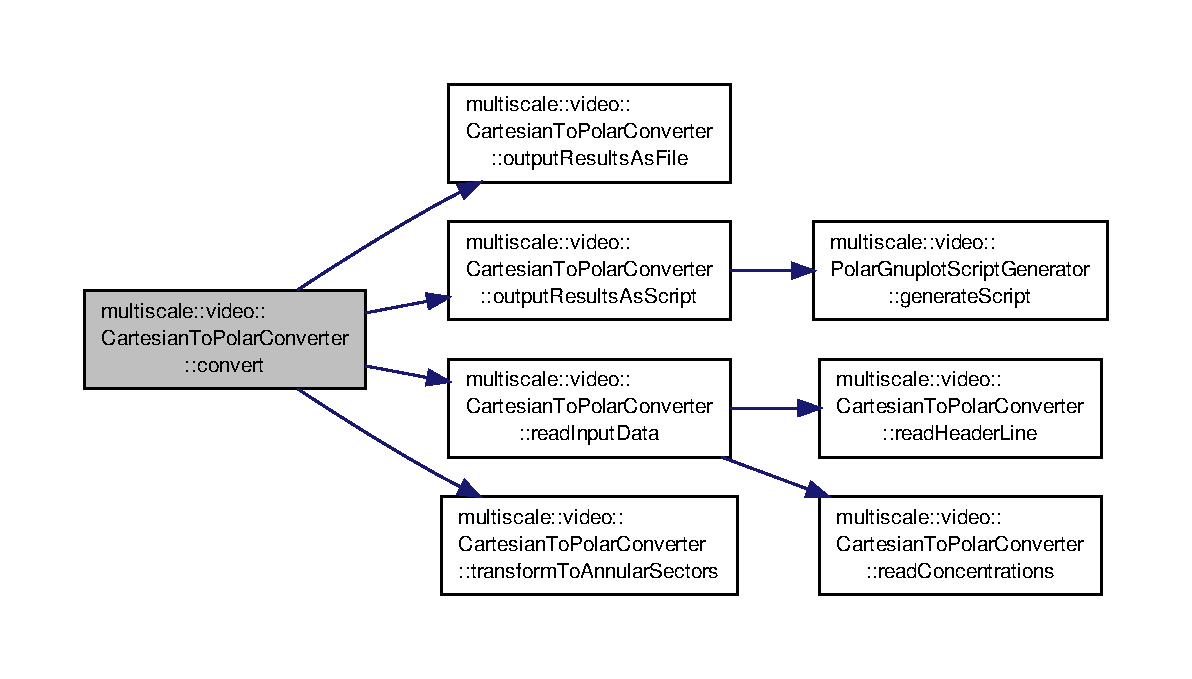
\includegraphics[width=350pt]{classmultiscale_1_1video_1_1CartesianToPolarConverter_aae3e7e842456da18741bccccdf084922_cgraph}
\end{center}
\end{figure}




\-Here is the caller graph for this function\-:
\nopagebreak
\begin{figure}[H]
\begin{center}
\leavevmode
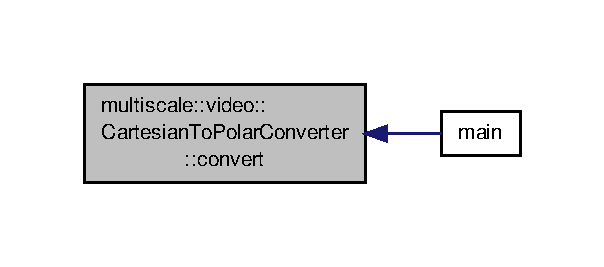
\includegraphics[width=350pt]{classmultiscale_1_1video_1_1CartesianToPolarConverter_aae3e7e842456da18741bccccdf084922_icgraph}
\end{center}
\end{figure}


\hypertarget{classmultiscale_1_1video_1_1CartesianToPolarConverter_adb3aeeb5f2994f8aa9dc03c8c8f270ad}{\index{multiscale\-::video\-::\-Cartesian\-To\-Polar\-Converter@{multiscale\-::video\-::\-Cartesian\-To\-Polar\-Converter}!output\-Results\-As\-File@{output\-Results\-As\-File}}
\index{output\-Results\-As\-File@{output\-Results\-As\-File}!multiscale::video::CartesianToPolarConverter@{multiscale\-::video\-::\-Cartesian\-To\-Polar\-Converter}}
\subsubsection[{output\-Results\-As\-File}]{\setlength{\rightskip}{0pt plus 5cm}void {\bf \-Cartesian\-To\-Polar\-Converter\-::output\-Results\-As\-File} (
\begin{DoxyParamCaption}
{}
\end{DoxyParamCaption}
)\hspace{0.3cm}{\ttfamily  \mbox{[}private\mbox{]}}}}\label{classmultiscale_1_1video_1_1CartesianToPolarConverter_adb3aeeb5f2994f8aa9dc03c8c8f270ad}


\-Output the results as a plain file. 



\-Definition at line 116 of file \-Cartesian\-To\-Polar\-Converter.\-cpp.



\-References annular\-Sectors, \-O\-U\-T\-P\-U\-T\-\_\-\-F\-I\-L\-E\-\_\-\-E\-X\-T\-E\-N\-S\-I\-O\-N, and output\-Filepath.



\-Referenced by convert().



\-Here is the caller graph for this function\-:
\nopagebreak
\begin{figure}[H]
\begin{center}
\leavevmode
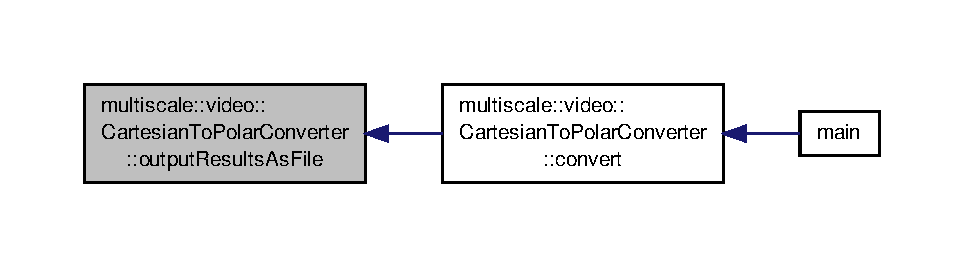
\includegraphics[width=350pt]{classmultiscale_1_1video_1_1CartesianToPolarConverter_adb3aeeb5f2994f8aa9dc03c8c8f270ad_icgraph}
\end{center}
\end{figure}


\hypertarget{classmultiscale_1_1video_1_1CartesianToPolarConverter_a680e357efb54b1193715259cb339516e}{\index{multiscale\-::video\-::\-Cartesian\-To\-Polar\-Converter@{multiscale\-::video\-::\-Cartesian\-To\-Polar\-Converter}!output\-Results\-As\-Script@{output\-Results\-As\-Script}}
\index{output\-Results\-As\-Script@{output\-Results\-As\-Script}!multiscale::video::CartesianToPolarConverter@{multiscale\-::video\-::\-Cartesian\-To\-Polar\-Converter}}
\subsubsection[{output\-Results\-As\-Script}]{\setlength{\rightskip}{0pt plus 5cm}void {\bf \-Cartesian\-To\-Polar\-Converter\-::output\-Results\-As\-Script} (
\begin{DoxyParamCaption}
{}
\end{DoxyParamCaption}
)\hspace{0.3cm}{\ttfamily  \mbox{[}private\mbox{]}}}}\label{classmultiscale_1_1video_1_1CartesianToPolarConverter_a680e357efb54b1193715259cb339516e}


\-Output the results as a gnuplot script. 



\-Definition at line 131 of file \-Cartesian\-To\-Polar\-Converter.\-cpp.



\-References annular\-Sectors, multiscale\-::video\-::\-Polar\-Gnuplot\-Script\-Generator\-::generate\-Script(), output\-Filepath, and simulation\-Time.



\-Referenced by convert().



\-Here is the call graph for this function\-:
\nopagebreak
\begin{figure}[H]
\begin{center}
\leavevmode
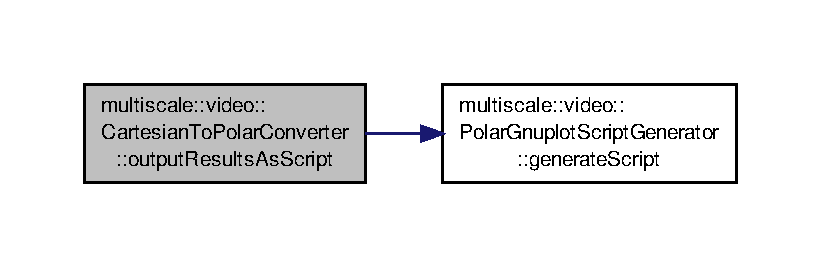
\includegraphics[width=350pt]{classmultiscale_1_1video_1_1CartesianToPolarConverter_a680e357efb54b1193715259cb339516e_cgraph}
\end{center}
\end{figure}




\-Here is the caller graph for this function\-:
\nopagebreak
\begin{figure}[H]
\begin{center}
\leavevmode
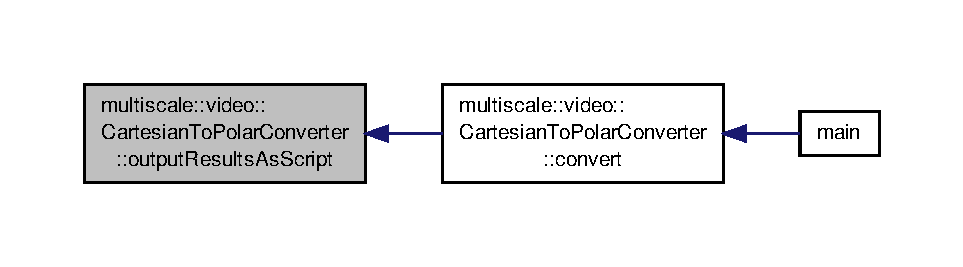
\includegraphics[width=350pt]{classmultiscale_1_1video_1_1CartesianToPolarConverter_a680e357efb54b1193715259cb339516e_icgraph}
\end{center}
\end{figure}


\hypertarget{classmultiscale_1_1video_1_1CartesianToPolarConverter_a7335cccc7e3c14203b00357ec6a2c140}{\index{multiscale\-::video\-::\-Cartesian\-To\-Polar\-Converter@{multiscale\-::video\-::\-Cartesian\-To\-Polar\-Converter}!read\-Concentrations@{read\-Concentrations}}
\index{read\-Concentrations@{read\-Concentrations}!multiscale::video::CartesianToPolarConverter@{multiscale\-::video\-::\-Cartesian\-To\-Polar\-Converter}}
\subsubsection[{read\-Concentrations}]{\setlength{\rightskip}{0pt plus 5cm}void {\bf \-Cartesian\-To\-Polar\-Converter\-::read\-Concentrations} (
\begin{DoxyParamCaption}
\item[{ifstream \&}]{fin}
\end{DoxyParamCaption}
)\hspace{0.3cm}{\ttfamily  \mbox{[}private\mbox{]}}}}\label{classmultiscale_1_1video_1_1CartesianToPolarConverter_a7335cccc7e3c14203b00357ec6a2c140}


\-Read the concentrations. 


\begin{DoxyParams}{\-Parameters}
{\em fin} & \-Input file stream \\
\hline
\end{DoxyParams}


\-Definition at line 71 of file \-Cartesian\-To\-Polar\-Converter.\-cpp.



\-References concentrations, \-E\-R\-R\-\_\-\-C\-O\-N\-C, \-M\-S\-\_\-throw, nr\-Of\-Concentric\-Circles, and nr\-Of\-Sectors.



\-Referenced by read\-Input\-Data().



\-Here is the caller graph for this function\-:
\nopagebreak
\begin{figure}[H]
\begin{center}
\leavevmode
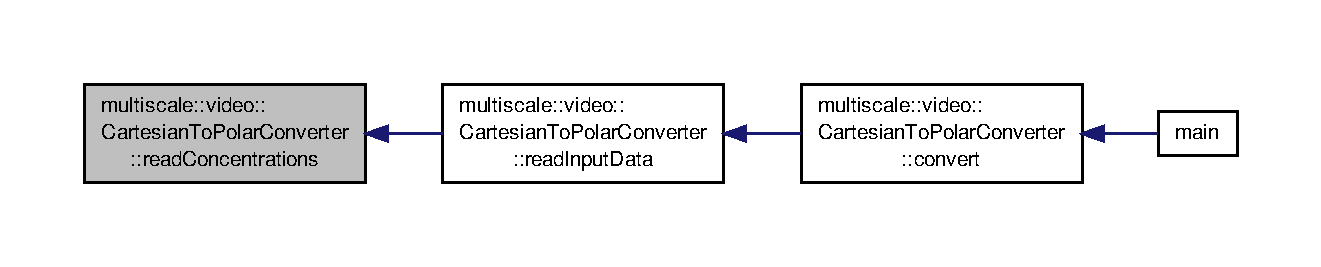
\includegraphics[width=350pt]{classmultiscale_1_1video_1_1CartesianToPolarConverter_a7335cccc7e3c14203b00357ec6a2c140_icgraph}
\end{center}
\end{figure}


\hypertarget{classmultiscale_1_1video_1_1CartesianToPolarConverter_a88d7c95fb76c9e139cb013c11a8dfae0}{\index{multiscale\-::video\-::\-Cartesian\-To\-Polar\-Converter@{multiscale\-::video\-::\-Cartesian\-To\-Polar\-Converter}!read\-Header\-Line@{read\-Header\-Line}}
\index{read\-Header\-Line@{read\-Header\-Line}!multiscale::video::CartesianToPolarConverter@{multiscale\-::video\-::\-Cartesian\-To\-Polar\-Converter}}
\subsubsection[{read\-Header\-Line}]{\setlength{\rightskip}{0pt plus 5cm}void {\bf \-Cartesian\-To\-Polar\-Converter\-::read\-Header\-Line} (
\begin{DoxyParamCaption}
\item[{ifstream \&}]{fin}
\end{DoxyParamCaption}
)\hspace{0.3cm}{\ttfamily  \mbox{[}private\mbox{]}}}}\label{classmultiscale_1_1video_1_1CartesianToPolarConverter_a88d7c95fb76c9e139cb013c11a8dfae0}


\-Read the header line. 

\-The header line contains values for number of concentric circles, number of sectors and simulation time


\begin{DoxyParams}{\-Parameters}
{\em fin} & \-Input file stream \\
\hline
\end{DoxyParams}


\-Definition at line 62 of file \-Cartesian\-To\-Polar\-Converter.\-cpp.



\-References \-E\-R\-R\-\_\-\-N\-E\-G\-\_\-\-S\-I\-M\-\_\-\-T\-I\-M\-E, \-E\-R\-R\-\_\-\-N\-O\-N\-P\-O\-S\-\_\-\-D\-I\-M\-E\-N\-S\-I\-O\-N, \-M\-S\-\_\-throw, nr\-Of\-Concentric\-Circles, nr\-Of\-Sectors, and simulation\-Time.



\-Referenced by read\-Input\-Data().



\-Here is the caller graph for this function\-:
\nopagebreak
\begin{figure}[H]
\begin{center}
\leavevmode
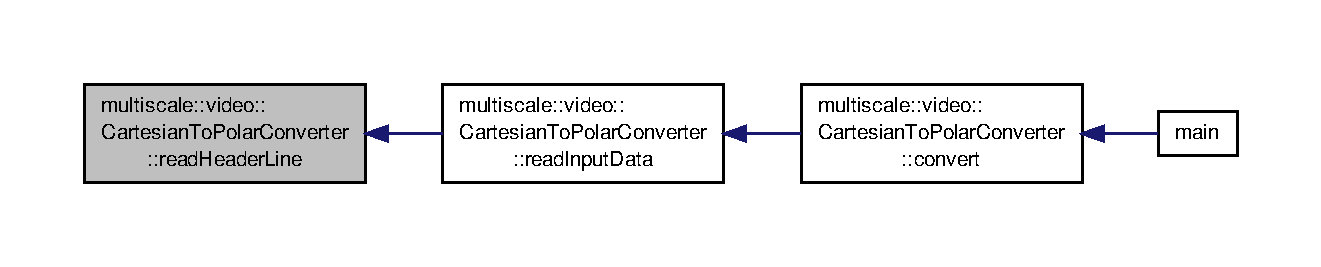
\includegraphics[width=350pt]{classmultiscale_1_1video_1_1CartesianToPolarConverter_a88d7c95fb76c9e139cb013c11a8dfae0_icgraph}
\end{center}
\end{figure}


\hypertarget{classmultiscale_1_1video_1_1CartesianToPolarConverter_a37891007ade23e05047d33d0c9cb3e13}{\index{multiscale\-::video\-::\-Cartesian\-To\-Polar\-Converter@{multiscale\-::video\-::\-Cartesian\-To\-Polar\-Converter}!read\-Input\-Data@{read\-Input\-Data}}
\index{read\-Input\-Data@{read\-Input\-Data}!multiscale::video::CartesianToPolarConverter@{multiscale\-::video\-::\-Cartesian\-To\-Polar\-Converter}}
\subsubsection[{read\-Input\-Data}]{\setlength{\rightskip}{0pt plus 5cm}void {\bf \-Cartesian\-To\-Polar\-Converter\-::read\-Input\-Data} (
\begin{DoxyParamCaption}
{}
\end{DoxyParamCaption}
)\hspace{0.3cm}{\ttfamily  \mbox{[}private\mbox{]}}}}\label{classmultiscale_1_1video_1_1CartesianToPolarConverter_a37891007ade23e05047d33d0c9cb3e13}


\-Read the input data. 



\-Definition at line 38 of file \-Cartesian\-To\-Polar\-Converter.\-cpp.



\-References \-E\-R\-R\-\_\-\-I\-N\-\_\-\-E\-X\-T\-R\-A\-\_\-\-D\-A\-T\-A, \-E\-R\-R\-\_\-\-I\-N\-P\-U\-T\-\_\-\-O\-P\-E\-N, input\-Filepath, \-M\-S\-\_\-throw, read\-Concentrations(), and read\-Header\-Line().



\-Referenced by convert().



\-Here is the call graph for this function\-:
\nopagebreak
\begin{figure}[H]
\begin{center}
\leavevmode
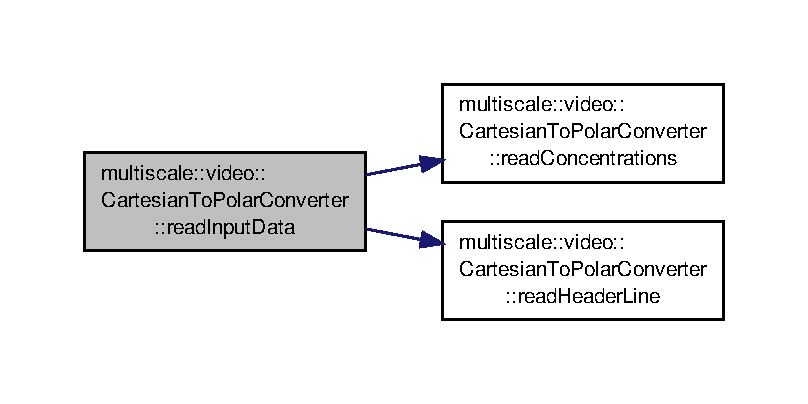
\includegraphics[width=350pt]{classmultiscale_1_1video_1_1CartesianToPolarConverter_a37891007ade23e05047d33d0c9cb3e13_cgraph}
\end{center}
\end{figure}




\-Here is the caller graph for this function\-:
\nopagebreak
\begin{figure}[H]
\begin{center}
\leavevmode
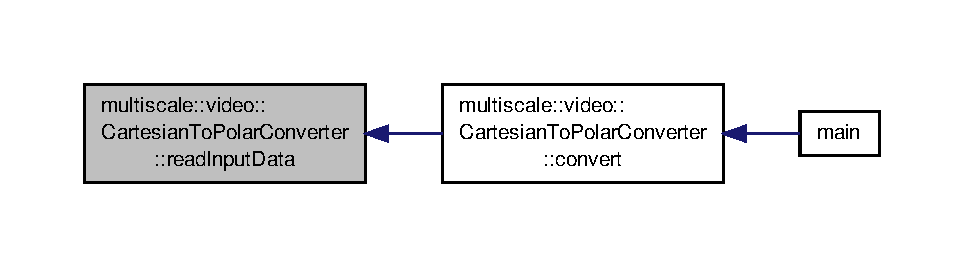
\includegraphics[width=350pt]{classmultiscale_1_1video_1_1CartesianToPolarConverter_a37891007ade23e05047d33d0c9cb3e13_icgraph}
\end{center}
\end{figure}


\hypertarget{classmultiscale_1_1video_1_1CartesianToPolarConverter_a0c3f499725a058d2a3251209d8c16178}{\index{multiscale\-::video\-::\-Cartesian\-To\-Polar\-Converter@{multiscale\-::video\-::\-Cartesian\-To\-Polar\-Converter}!transform\-To\-Annular\-Sectors@{transform\-To\-Annular\-Sectors}}
\index{transform\-To\-Annular\-Sectors@{transform\-To\-Annular\-Sectors}!multiscale::video::CartesianToPolarConverter@{multiscale\-::video\-::\-Cartesian\-To\-Polar\-Converter}}
\subsubsection[{transform\-To\-Annular\-Sectors}]{\setlength{\rightskip}{0pt plus 5cm}void {\bf \-Cartesian\-To\-Polar\-Converter\-::transform\-To\-Annular\-Sectors} (
\begin{DoxyParamCaption}
{}
\end{DoxyParamCaption}
)\hspace{0.3cm}{\ttfamily  \mbox{[}private\mbox{]}}}}\label{classmultiscale_1_1video_1_1CartesianToPolarConverter_a0c3f499725a058d2a3251209d8c16178}


\-Convert the concentrations to annular sectors. 



\-Definition at line 91 of file \-Cartesian\-To\-Polar\-Converter.\-cpp.



\-References annular\-Sectors, concentrations, nr\-Of\-Concentric\-Circles, nr\-Of\-Sectors, \-R\-A\-D\-I\-U\-S\-\_\-\-M\-A\-X, and \-R\-A\-D\-I\-U\-S\-\_\-\-M\-I\-N.



\-Referenced by convert().



\-Here is the caller graph for this function\-:
\nopagebreak
\begin{figure}[H]
\begin{center}
\leavevmode
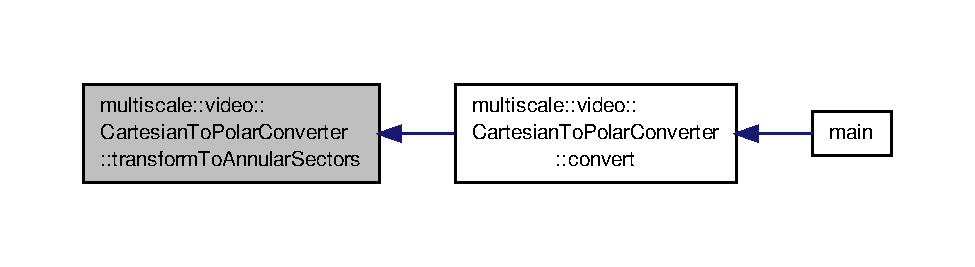
\includegraphics[width=350pt]{classmultiscale_1_1video_1_1CartesianToPolarConverter_a0c3f499725a058d2a3251209d8c16178_icgraph}
\end{center}
\end{figure}




\subsection{\-Member \-Data \-Documentation}
\hypertarget{classmultiscale_1_1video_1_1CartesianToPolarConverter_a3f8004ac5f8bae93c7a5e09bc37ba0ac}{\index{multiscale\-::video\-::\-Cartesian\-To\-Polar\-Converter@{multiscale\-::video\-::\-Cartesian\-To\-Polar\-Converter}!annular\-Sectors@{annular\-Sectors}}
\index{annular\-Sectors@{annular\-Sectors}!multiscale::video::CartesianToPolarConverter@{multiscale\-::video\-::\-Cartesian\-To\-Polar\-Converter}}
\subsubsection[{annular\-Sectors}]{\setlength{\rightskip}{0pt plus 5cm}vector$<${\bf \-Annular\-Sector}$>$ {\bf multiscale\-::video\-::\-Cartesian\-To\-Polar\-Converter\-::annular\-Sectors}\hspace{0.3cm}{\ttfamily  \mbox{[}private\mbox{]}}}}\label{classmultiscale_1_1video_1_1CartesianToPolarConverter_a3f8004ac5f8bae93c7a5e09bc37ba0ac}
\-Resulting annular sectors 

\-Definition at line 21 of file \-Cartesian\-To\-Polar\-Converter.\-hpp.



\-Referenced by output\-Results\-As\-File(), output\-Results\-As\-Script(), and transform\-To\-Annular\-Sectors().

\hypertarget{classmultiscale_1_1video_1_1CartesianToPolarConverter_a7356e201623f518132d75b7bc48407d3}{\index{multiscale\-::video\-::\-Cartesian\-To\-Polar\-Converter@{multiscale\-::video\-::\-Cartesian\-To\-Polar\-Converter}!concentrations@{concentrations}}
\index{concentrations@{concentrations}!multiscale::video::CartesianToPolarConverter@{multiscale\-::video\-::\-Cartesian\-To\-Polar\-Converter}}
\subsubsection[{concentrations}]{\setlength{\rightskip}{0pt plus 5cm}vector$<$double$>$ {\bf multiscale\-::video\-::\-Cartesian\-To\-Polar\-Converter\-::concentrations}\hspace{0.3cm}{\ttfamily  \mbox{[}private\mbox{]}}}}\label{classmultiscale_1_1video_1_1CartesianToPolarConverter_a7356e201623f518132d75b7bc48407d3}
\-Concentrations received as input 

\-Definition at line 22 of file \-Cartesian\-To\-Polar\-Converter.\-hpp.



\-Referenced by read\-Concentrations(), and transform\-To\-Annular\-Sectors().

\hypertarget{classmultiscale_1_1video_1_1CartesianToPolarConverter_a2657e7972c2d3f7cc4c0011ccd8423e4}{\index{multiscale\-::video\-::\-Cartesian\-To\-Polar\-Converter@{multiscale\-::video\-::\-Cartesian\-To\-Polar\-Converter}!\-E\-R\-R\-\_\-\-C\-O\-N\-C@{\-E\-R\-R\-\_\-\-C\-O\-N\-C}}
\index{\-E\-R\-R\-\_\-\-C\-O\-N\-C@{\-E\-R\-R\-\_\-\-C\-O\-N\-C}!multiscale::video::CartesianToPolarConverter@{multiscale\-::video\-::\-Cartesian\-To\-Polar\-Converter}}
\subsubsection[{\-E\-R\-R\-\_\-\-C\-O\-N\-C}]{\setlength{\rightskip}{0pt plus 5cm}const string {\bf \-Cartesian\-To\-Polar\-Converter\-::\-E\-R\-R\-\_\-\-C\-O\-N\-C} = \char`\"{}\-All {\bf concentrations} have to be between 0 and 1.\char`\"{}\hspace{0.3cm}{\ttfamily  \mbox{[}static, private\mbox{]}}}}\label{classmultiscale_1_1video_1_1CartesianToPolarConverter_a2657e7972c2d3f7cc4c0011ccd8423e4}


\-Definition at line 74 of file \-Cartesian\-To\-Polar\-Converter.\-hpp.



\-Referenced by read\-Concentrations().

\hypertarget{classmultiscale_1_1video_1_1CartesianToPolarConverter_a27c4664c63c53cc5351bbb3233bdfce1}{\index{multiscale\-::video\-::\-Cartesian\-To\-Polar\-Converter@{multiscale\-::video\-::\-Cartesian\-To\-Polar\-Converter}!\-E\-R\-R\-\_\-\-I\-N\-\_\-\-E\-X\-T\-R\-A\-\_\-\-D\-A\-T\-A@{\-E\-R\-R\-\_\-\-I\-N\-\_\-\-E\-X\-T\-R\-A\-\_\-\-D\-A\-T\-A}}
\index{\-E\-R\-R\-\_\-\-I\-N\-\_\-\-E\-X\-T\-R\-A\-\_\-\-D\-A\-T\-A@{\-E\-R\-R\-\_\-\-I\-N\-\_\-\-E\-X\-T\-R\-A\-\_\-\-D\-A\-T\-A}!multiscale::video::CartesianToPolarConverter@{multiscale\-::video\-::\-Cartesian\-To\-Polar\-Converter}}
\subsubsection[{\-E\-R\-R\-\_\-\-I\-N\-\_\-\-E\-X\-T\-R\-A\-\_\-\-D\-A\-T\-A}]{\setlength{\rightskip}{0pt plus 5cm}const string {\bf \-Cartesian\-To\-Polar\-Converter\-::\-E\-R\-R\-\_\-\-I\-N\-\_\-\-E\-X\-T\-R\-A\-\_\-\-D\-A\-T\-A} = \char`\"{}\-The input file contains more data than required.\char`\"{}\hspace{0.3cm}{\ttfamily  \mbox{[}static, private\mbox{]}}}}\label{classmultiscale_1_1video_1_1CartesianToPolarConverter_a27c4664c63c53cc5351bbb3233bdfce1}


\-Definition at line 78 of file \-Cartesian\-To\-Polar\-Converter.\-hpp.



\-Referenced by read\-Input\-Data().

\hypertarget{classmultiscale_1_1video_1_1CartesianToPolarConverter_a298f7aba7ec17e486484fa2e52ebc109}{\index{multiscale\-::video\-::\-Cartesian\-To\-Polar\-Converter@{multiscale\-::video\-::\-Cartesian\-To\-Polar\-Converter}!\-E\-R\-R\-\_\-\-I\-N\-P\-U\-T\-\_\-\-O\-P\-E\-N@{\-E\-R\-R\-\_\-\-I\-N\-P\-U\-T\-\_\-\-O\-P\-E\-N}}
\index{\-E\-R\-R\-\_\-\-I\-N\-P\-U\-T\-\_\-\-O\-P\-E\-N@{\-E\-R\-R\-\_\-\-I\-N\-P\-U\-T\-\_\-\-O\-P\-E\-N}!multiscale::video::CartesianToPolarConverter@{multiscale\-::video\-::\-Cartesian\-To\-Polar\-Converter}}
\subsubsection[{\-E\-R\-R\-\_\-\-I\-N\-P\-U\-T\-\_\-\-O\-P\-E\-N}]{\setlength{\rightskip}{0pt plus 5cm}const string {\bf \-Cartesian\-To\-Polar\-Converter\-::\-E\-R\-R\-\_\-\-I\-N\-P\-U\-T\-\_\-\-O\-P\-E\-N} = \char`\"{}\-The input file could not be opened\char`\"{}\hspace{0.3cm}{\ttfamily  \mbox{[}static, private\mbox{]}}}}\label{classmultiscale_1_1video_1_1CartesianToPolarConverter_a298f7aba7ec17e486484fa2e52ebc109}


\-Definition at line 77 of file \-Cartesian\-To\-Polar\-Converter.\-hpp.



\-Referenced by read\-Input\-Data().

\hypertarget{classmultiscale_1_1video_1_1CartesianToPolarConverter_a0a3ab913d167193883dc96aed6cc8290}{\index{multiscale\-::video\-::\-Cartesian\-To\-Polar\-Converter@{multiscale\-::video\-::\-Cartesian\-To\-Polar\-Converter}!\-E\-R\-R\-\_\-\-N\-E\-G\-\_\-\-S\-I\-M\-\_\-\-T\-I\-M\-E@{\-E\-R\-R\-\_\-\-N\-E\-G\-\_\-\-S\-I\-M\-\_\-\-T\-I\-M\-E}}
\index{\-E\-R\-R\-\_\-\-N\-E\-G\-\_\-\-S\-I\-M\-\_\-\-T\-I\-M\-E@{\-E\-R\-R\-\_\-\-N\-E\-G\-\_\-\-S\-I\-M\-\_\-\-T\-I\-M\-E}!multiscale::video::CartesianToPolarConverter@{multiscale\-::video\-::\-Cartesian\-To\-Polar\-Converter}}
\subsubsection[{\-E\-R\-R\-\_\-\-N\-E\-G\-\_\-\-S\-I\-M\-\_\-\-T\-I\-M\-E}]{\setlength{\rightskip}{0pt plus 5cm}const string {\bf \-Cartesian\-To\-Polar\-Converter\-::\-E\-R\-R\-\_\-\-N\-E\-G\-\_\-\-S\-I\-M\-\_\-\-T\-I\-M\-E} = \char`\"{}\-The simulation time must be non-\/negative.\char`\"{}\hspace{0.3cm}{\ttfamily  \mbox{[}static, private\mbox{]}}}}\label{classmultiscale_1_1video_1_1CartesianToPolarConverter_a0a3ab913d167193883dc96aed6cc8290}


\-Definition at line 76 of file \-Cartesian\-To\-Polar\-Converter.\-hpp.



\-Referenced by read\-Header\-Line().

\hypertarget{classmultiscale_1_1video_1_1CartesianToPolarConverter_ab3a2114f4dd2615abba3305609f1b616}{\index{multiscale\-::video\-::\-Cartesian\-To\-Polar\-Converter@{multiscale\-::video\-::\-Cartesian\-To\-Polar\-Converter}!\-E\-R\-R\-\_\-\-N\-O\-N\-P\-O\-S\-\_\-\-D\-I\-M\-E\-N\-S\-I\-O\-N@{\-E\-R\-R\-\_\-\-N\-O\-N\-P\-O\-S\-\_\-\-D\-I\-M\-E\-N\-S\-I\-O\-N}}
\index{\-E\-R\-R\-\_\-\-N\-O\-N\-P\-O\-S\-\_\-\-D\-I\-M\-E\-N\-S\-I\-O\-N@{\-E\-R\-R\-\_\-\-N\-O\-N\-P\-O\-S\-\_\-\-D\-I\-M\-E\-N\-S\-I\-O\-N}!multiscale::video::CartesianToPolarConverter@{multiscale\-::video\-::\-Cartesian\-To\-Polar\-Converter}}
\subsubsection[{\-E\-R\-R\-\_\-\-N\-O\-N\-P\-O\-S\-\_\-\-D\-I\-M\-E\-N\-S\-I\-O\-N}]{\setlength{\rightskip}{0pt plus 5cm}const string {\bf \-Cartesian\-To\-Polar\-Converter\-::\-E\-R\-R\-\_\-\-N\-O\-N\-P\-O\-S\-\_\-\-D\-I\-M\-E\-N\-S\-I\-O\-N} = \char`\"{}\-The dimensions \-N and \-M must be positive.\char`\"{}\hspace{0.3cm}{\ttfamily  \mbox{[}static, private\mbox{]}}}}\label{classmultiscale_1_1video_1_1CartesianToPolarConverter_ab3a2114f4dd2615abba3305609f1b616}


\-Definition at line 75 of file \-Cartesian\-To\-Polar\-Converter.\-hpp.



\-Referenced by read\-Header\-Line().

\hypertarget{classmultiscale_1_1video_1_1CartesianToPolarConverter_aa15eca9e8d3da0eb8ff1b6583e392f05}{\index{multiscale\-::video\-::\-Cartesian\-To\-Polar\-Converter@{multiscale\-::video\-::\-Cartesian\-To\-Polar\-Converter}!input\-Filepath@{input\-Filepath}}
\index{input\-Filepath@{input\-Filepath}!multiscale::video::CartesianToPolarConverter@{multiscale\-::video\-::\-Cartesian\-To\-Polar\-Converter}}
\subsubsection[{input\-Filepath}]{\setlength{\rightskip}{0pt plus 5cm}string {\bf multiscale\-::video\-::\-Cartesian\-To\-Polar\-Converter\-::input\-Filepath}\hspace{0.3cm}{\ttfamily  \mbox{[}private\mbox{]}}}}\label{classmultiscale_1_1video_1_1CartesianToPolarConverter_aa15eca9e8d3da0eb8ff1b6583e392f05}
\-Path to the input file 

\-Definition at line 28 of file \-Cartesian\-To\-Polar\-Converter.\-hpp.



\-Referenced by read\-Input\-Data().

\hypertarget{classmultiscale_1_1video_1_1CartesianToPolarConverter_ab7c8564deaa38c57a251ba9592903238}{\index{multiscale\-::video\-::\-Cartesian\-To\-Polar\-Converter@{multiscale\-::video\-::\-Cartesian\-To\-Polar\-Converter}!nr\-Of\-Concentric\-Circles@{nr\-Of\-Concentric\-Circles}}
\index{nr\-Of\-Concentric\-Circles@{nr\-Of\-Concentric\-Circles}!multiscale::video::CartesianToPolarConverter@{multiscale\-::video\-::\-Cartesian\-To\-Polar\-Converter}}
\subsubsection[{nr\-Of\-Concentric\-Circles}]{\setlength{\rightskip}{0pt plus 5cm}unsigned long {\bf multiscale\-::video\-::\-Cartesian\-To\-Polar\-Converter\-::nr\-Of\-Concentric\-Circles}\hspace{0.3cm}{\ttfamily  \mbox{[}private\mbox{]}}}}\label{classmultiscale_1_1video_1_1CartesianToPolarConverter_ab7c8564deaa38c57a251ba9592903238}
\-Number of concentric circles 

\-Definition at line 24 of file \-Cartesian\-To\-Polar\-Converter.\-hpp.



\-Referenced by \-Cartesian\-To\-Polar\-Converter(), read\-Concentrations(), read\-Header\-Line(), and transform\-To\-Annular\-Sectors().

\hypertarget{classmultiscale_1_1video_1_1CartesianToPolarConverter_a62a2f5abe655f440e7c41fe834f828d0}{\index{multiscale\-::video\-::\-Cartesian\-To\-Polar\-Converter@{multiscale\-::video\-::\-Cartesian\-To\-Polar\-Converter}!nr\-Of\-Sectors@{nr\-Of\-Sectors}}
\index{nr\-Of\-Sectors@{nr\-Of\-Sectors}!multiscale::video::CartesianToPolarConverter@{multiscale\-::video\-::\-Cartesian\-To\-Polar\-Converter}}
\subsubsection[{nr\-Of\-Sectors}]{\setlength{\rightskip}{0pt plus 5cm}unsigned long {\bf multiscale\-::video\-::\-Cartesian\-To\-Polar\-Converter\-::nr\-Of\-Sectors}\hspace{0.3cm}{\ttfamily  \mbox{[}private\mbox{]}}}}\label{classmultiscale_1_1video_1_1CartesianToPolarConverter_a62a2f5abe655f440e7c41fe834f828d0}
\-Number of sectors 

\-Definition at line 25 of file \-Cartesian\-To\-Polar\-Converter.\-hpp.



\-Referenced by \-Cartesian\-To\-Polar\-Converter(), read\-Concentrations(), read\-Header\-Line(), and transform\-To\-Annular\-Sectors().

\hypertarget{classmultiscale_1_1video_1_1CartesianToPolarConverter_a3dcad19e1da427627d783a3053174372}{\index{multiscale\-::video\-::\-Cartesian\-To\-Polar\-Converter@{multiscale\-::video\-::\-Cartesian\-To\-Polar\-Converter}!\-O\-U\-T\-P\-U\-T\-\_\-\-F\-I\-L\-E\-\_\-\-E\-X\-T\-E\-N\-S\-I\-O\-N@{\-O\-U\-T\-P\-U\-T\-\_\-\-F\-I\-L\-E\-\_\-\-E\-X\-T\-E\-N\-S\-I\-O\-N}}
\index{\-O\-U\-T\-P\-U\-T\-\_\-\-F\-I\-L\-E\-\_\-\-E\-X\-T\-E\-N\-S\-I\-O\-N@{\-O\-U\-T\-P\-U\-T\-\_\-\-F\-I\-L\-E\-\_\-\-E\-X\-T\-E\-N\-S\-I\-O\-N}!multiscale::video::CartesianToPolarConverter@{multiscale\-::video\-::\-Cartesian\-To\-Polar\-Converter}}
\subsubsection[{\-O\-U\-T\-P\-U\-T\-\_\-\-F\-I\-L\-E\-\_\-\-E\-X\-T\-E\-N\-S\-I\-O\-N}]{\setlength{\rightskip}{0pt plus 5cm}const string {\bf \-Cartesian\-To\-Polar\-Converter\-::\-O\-U\-T\-P\-U\-T\-\_\-\-F\-I\-L\-E\-\_\-\-E\-X\-T\-E\-N\-S\-I\-O\-N} = \char`\"{}.out\char`\"{}\hspace{0.3cm}{\ttfamily  \mbox{[}static, private\mbox{]}}}}\label{classmultiscale_1_1video_1_1CartesianToPolarConverter_a3dcad19e1da427627d783a3053174372}


\-Definition at line 80 of file \-Cartesian\-To\-Polar\-Converter.\-hpp.



\-Referenced by output\-Results\-As\-File().

\hypertarget{classmultiscale_1_1video_1_1CartesianToPolarConverter_a024d95ab3b9de6ed6fd1d951c5575e65}{\index{multiscale\-::video\-::\-Cartesian\-To\-Polar\-Converter@{multiscale\-::video\-::\-Cartesian\-To\-Polar\-Converter}!output\-Filepath@{output\-Filepath}}
\index{output\-Filepath@{output\-Filepath}!multiscale::video::CartesianToPolarConverter@{multiscale\-::video\-::\-Cartesian\-To\-Polar\-Converter}}
\subsubsection[{output\-Filepath}]{\setlength{\rightskip}{0pt plus 5cm}string {\bf multiscale\-::video\-::\-Cartesian\-To\-Polar\-Converter\-::output\-Filepath}\hspace{0.3cm}{\ttfamily  \mbox{[}private\mbox{]}}}}\label{classmultiscale_1_1video_1_1CartesianToPolarConverter_a024d95ab3b9de6ed6fd1d951c5575e65}
\-Path to the output file 

\-Definition at line 29 of file \-Cartesian\-To\-Polar\-Converter.\-hpp.



\-Referenced by output\-Results\-As\-File(), and output\-Results\-As\-Script().

\hypertarget{classmultiscale_1_1video_1_1CartesianToPolarConverter_a79bb03defe0d68884ce5d4f1b0a7d60c}{\index{multiscale\-::video\-::\-Cartesian\-To\-Polar\-Converter@{multiscale\-::video\-::\-Cartesian\-To\-Polar\-Converter}!\-R\-A\-D\-I\-U\-S\-\_\-\-M\-A\-X@{\-R\-A\-D\-I\-U\-S\-\_\-\-M\-A\-X}}
\index{\-R\-A\-D\-I\-U\-S\-\_\-\-M\-A\-X@{\-R\-A\-D\-I\-U\-S\-\_\-\-M\-A\-X}!multiscale::video::CartesianToPolarConverter@{multiscale\-::video\-::\-Cartesian\-To\-Polar\-Converter}}
\subsubsection[{\-R\-A\-D\-I\-U\-S\-\_\-\-M\-A\-X}]{\setlength{\rightskip}{0pt plus 5cm}const double {\bf \-Cartesian\-To\-Polar\-Converter\-::\-R\-A\-D\-I\-U\-S\-\_\-\-M\-A\-X} = 0.\-3\hspace{0.3cm}{\ttfamily  \mbox{[}static, private\mbox{]}}}}\label{classmultiscale_1_1video_1_1CartesianToPolarConverter_a79bb03defe0d68884ce5d4f1b0a7d60c}


\-Definition at line 83 of file \-Cartesian\-To\-Polar\-Converter.\-hpp.



\-Referenced by transform\-To\-Annular\-Sectors().

\hypertarget{classmultiscale_1_1video_1_1CartesianToPolarConverter_a59c18c22603ad65bf26533dd2aafd04e}{\index{multiscale\-::video\-::\-Cartesian\-To\-Polar\-Converter@{multiscale\-::video\-::\-Cartesian\-To\-Polar\-Converter}!\-R\-A\-D\-I\-U\-S\-\_\-\-M\-I\-N@{\-R\-A\-D\-I\-U\-S\-\_\-\-M\-I\-N}}
\index{\-R\-A\-D\-I\-U\-S\-\_\-\-M\-I\-N@{\-R\-A\-D\-I\-U\-S\-\_\-\-M\-I\-N}!multiscale::video::CartesianToPolarConverter@{multiscale\-::video\-::\-Cartesian\-To\-Polar\-Converter}}
\subsubsection[{\-R\-A\-D\-I\-U\-S\-\_\-\-M\-I\-N}]{\setlength{\rightskip}{0pt plus 5cm}const double {\bf \-Cartesian\-To\-Polar\-Converter\-::\-R\-A\-D\-I\-U\-S\-\_\-\-M\-I\-N} = 0.\-001\hspace{0.3cm}{\ttfamily  \mbox{[}static, private\mbox{]}}}}\label{classmultiscale_1_1video_1_1CartesianToPolarConverter_a59c18c22603ad65bf26533dd2aafd04e}


\-Definition at line 82 of file \-Cartesian\-To\-Polar\-Converter.\-hpp.



\-Referenced by transform\-To\-Annular\-Sectors().

\hypertarget{classmultiscale_1_1video_1_1CartesianToPolarConverter_a78003dc9053d89f56c03408f7f8fedda}{\index{multiscale\-::video\-::\-Cartesian\-To\-Polar\-Converter@{multiscale\-::video\-::\-Cartesian\-To\-Polar\-Converter}!simulation\-Time@{simulation\-Time}}
\index{simulation\-Time@{simulation\-Time}!multiscale::video::CartesianToPolarConverter@{multiscale\-::video\-::\-Cartesian\-To\-Polar\-Converter}}
\subsubsection[{simulation\-Time}]{\setlength{\rightskip}{0pt plus 5cm}double {\bf multiscale\-::video\-::\-Cartesian\-To\-Polar\-Converter\-::simulation\-Time}\hspace{0.3cm}{\ttfamily  \mbox{[}private\mbox{]}}}}\label{classmultiscale_1_1video_1_1CartesianToPolarConverter_a78003dc9053d89f56c03408f7f8fedda}
\-Simulation time corresponding to the input data 

\-Definition at line 26 of file \-Cartesian\-To\-Polar\-Converter.\-hpp.



\-Referenced by \-Cartesian\-To\-Polar\-Converter(), output\-Results\-As\-Script(), and read\-Header\-Line().



\-The documentation for this class was generated from the following files\-:\begin{DoxyCompactItemize}
\item 
/home/ovidiu/\-Repositories/git/multiscale/\-Multiscale/modules/video/circular/include/multiscale/video/circular/\hyperlink{CartesianToPolarConverter_8hpp}{\-Cartesian\-To\-Polar\-Converter.\-hpp}\item 
/home/ovidiu/\-Repositories/git/multiscale/\-Multiscale/modules/video/circular/src/\hyperlink{CartesianToPolarConverter_8cpp}{\-Cartesian\-To\-Polar\-Converter.\-cpp}\end{DoxyCompactItemize}

\hypertarget{classmultiscale_1_1CartesianToPolarConverterException}{\section{multiscale\-:\-:Cartesian\-To\-Polar\-Converter\-Exception Class Reference}
\label{classmultiscale_1_1CartesianToPolarConverterException}\index{multiscale\-::\-Cartesian\-To\-Polar\-Converter\-Exception@{multiscale\-::\-Cartesian\-To\-Polar\-Converter\-Exception}}
}


Exception class for the Cartesian\-To\-Polar\-Converter class.  




{\ttfamily \#include $<$Cartesian\-To\-Polar\-Converter\-Exception.\-hpp$>$}



Inheritance diagram for multiscale\-:\-:Cartesian\-To\-Polar\-Converter\-Exception\-:\nopagebreak
\begin{figure}[H]
\begin{center}
\leavevmode
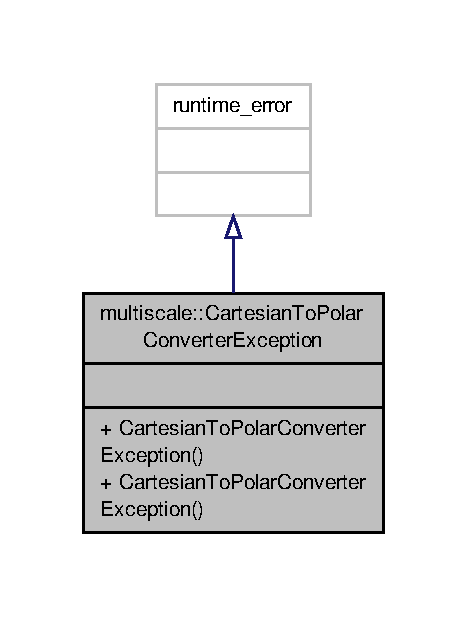
\includegraphics[width=234pt]{classmultiscale_1_1CartesianToPolarConverterException__inherit__graph}
\end{center}
\end{figure}


Collaboration diagram for multiscale\-:\-:Cartesian\-To\-Polar\-Converter\-Exception\-:\nopagebreak
\begin{figure}[H]
\begin{center}
\leavevmode
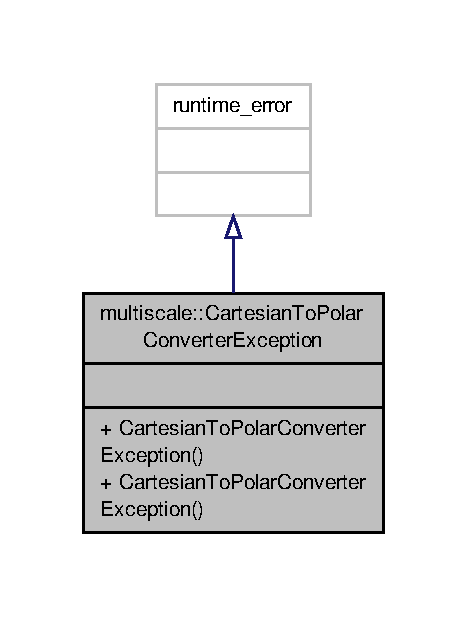
\includegraphics[width=234pt]{classmultiscale_1_1CartesianToPolarConverterException__coll__graph}
\end{center}
\end{figure}
\subsection*{Public Member Functions}
\begin{DoxyCompactItemize}
\item 
\hyperlink{classmultiscale_1_1CartesianToPolarConverterException_a70f2259e58ab16d64d88e8728fd67f26}{Cartesian\-To\-Polar\-Converter\-Exception} (const string \&file, int line, const string \&msg)
\item 
\hyperlink{classmultiscale_1_1CartesianToPolarConverterException_a9d77f79a95ff2557a6cd5060021c70c2}{Cartesian\-To\-Polar\-Converter\-Exception} (const string \&file, int line, const char $\ast$msg)
\end{DoxyCompactItemize}


\subsection{Detailed Description}
Exception class for the Cartesian\-To\-Polar\-Converter class. 

Definition at line 14 of file Cartesian\-To\-Polar\-Converter\-Exception.\-hpp.



\subsection{Constructor \& Destructor Documentation}
\hypertarget{classmultiscale_1_1CartesianToPolarConverterException_a70f2259e58ab16d64d88e8728fd67f26}{\index{multiscale\-::\-Cartesian\-To\-Polar\-Converter\-Exception@{multiscale\-::\-Cartesian\-To\-Polar\-Converter\-Exception}!Cartesian\-To\-Polar\-Converter\-Exception@{Cartesian\-To\-Polar\-Converter\-Exception}}
\index{Cartesian\-To\-Polar\-Converter\-Exception@{Cartesian\-To\-Polar\-Converter\-Exception}!multiscale::CartesianToPolarConverterException@{multiscale\-::\-Cartesian\-To\-Polar\-Converter\-Exception}}
\subsubsection[{Cartesian\-To\-Polar\-Converter\-Exception}]{\setlength{\rightskip}{0pt plus 5cm}multiscale\-::\-Cartesian\-To\-Polar\-Converter\-Exception\-::\-Cartesian\-To\-Polar\-Converter\-Exception (
\begin{DoxyParamCaption}
\item[{const string \&}]{file, }
\item[{int}]{line, }
\item[{const string \&}]{msg}
\end{DoxyParamCaption}
)\hspace{0.3cm}{\ttfamily [inline]}}}\label{classmultiscale_1_1CartesianToPolarConverterException_a70f2259e58ab16d64d88e8728fd67f26}


Definition at line 18 of file Cartesian\-To\-Polar\-Converter\-Exception.\-hpp.

\hypertarget{classmultiscale_1_1CartesianToPolarConverterException_a9d77f79a95ff2557a6cd5060021c70c2}{\index{multiscale\-::\-Cartesian\-To\-Polar\-Converter\-Exception@{multiscale\-::\-Cartesian\-To\-Polar\-Converter\-Exception}!Cartesian\-To\-Polar\-Converter\-Exception@{Cartesian\-To\-Polar\-Converter\-Exception}}
\index{Cartesian\-To\-Polar\-Converter\-Exception@{Cartesian\-To\-Polar\-Converter\-Exception}!multiscale::CartesianToPolarConverterException@{multiscale\-::\-Cartesian\-To\-Polar\-Converter\-Exception}}
\subsubsection[{Cartesian\-To\-Polar\-Converter\-Exception}]{\setlength{\rightskip}{0pt plus 5cm}multiscale\-::\-Cartesian\-To\-Polar\-Converter\-Exception\-::\-Cartesian\-To\-Polar\-Converter\-Exception (
\begin{DoxyParamCaption}
\item[{const string \&}]{file, }
\item[{int}]{line, }
\item[{const char $\ast$}]{msg}
\end{DoxyParamCaption}
)\hspace{0.3cm}{\ttfamily [inline]}}}\label{classmultiscale_1_1CartesianToPolarConverterException_a9d77f79a95ff2557a6cd5060021c70c2}


Definition at line 20 of file Cartesian\-To\-Polar\-Converter\-Exception.\-hpp.



The documentation for this class was generated from the following file\-:\begin{DoxyCompactItemize}
\item 
include/multiscale/exception/\hyperlink{CartesianToPolarConverterException_8hpp}{Cartesian\-To\-Polar\-Converter\-Exception.\-hpp}\end{DoxyCompactItemize}

\hypertarget{classmultiscale_1_1analysis_1_1CircularityMeasure}{\section{multiscale\-:\-:analysis\-:\-:Circularity\-Measure Class Reference}
\label{classmultiscale_1_1analysis_1_1CircularityMeasure}\index{multiscale\-::analysis\-::\-Circularity\-Measure@{multiscale\-::analysis\-::\-Circularity\-Measure}}
}


Class for computing the circularity measure for the given collection of points.  




{\ttfamily \#include $<$Circularity\-Measure.\-hpp$>$}



Collaboration diagram for multiscale\-:\-:analysis\-:\-:Circularity\-Measure\-:
\nopagebreak
\begin{figure}[H]
\begin{center}
\leavevmode
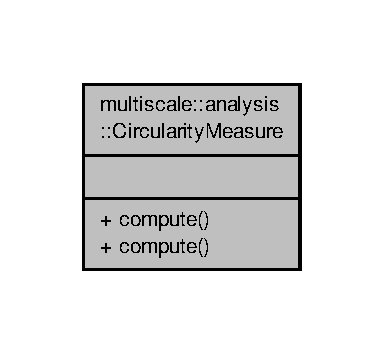
\includegraphics[width=184pt]{classmultiscale_1_1analysis_1_1CircularityMeasure__coll__graph}
\end{center}
\end{figure}
\subsection*{Static Public Member Functions}
\begin{DoxyCompactItemize}
\item 
static double \hyperlink{classmultiscale_1_1analysis_1_1CircularityMeasure_a819f1b1f9d7cdd96de2a6d9c5b6c6caa}{compute} (const vector$<$ Point2f $>$ \&points)
\begin{DoxyCompactList}\small\item\em Compute circularity measure for the given collection of points. \end{DoxyCompactList}\item 
static double \hyperlink{classmultiscale_1_1analysis_1_1CircularityMeasure_a252830f574cd4a85f108f74265520a8f}{compute} (const vector$<$ Point $>$ \&points)
\begin{DoxyCompactList}\small\item\em Compute circularity measure for the given collection of points. \end{DoxyCompactList}\end{DoxyCompactItemize}


\subsection{Detailed Description}
Class for computing the circularity measure for the given collection of points. 

Definition at line 18 of file Circularity\-Measure.\-hpp.



\subsection{Member Function Documentation}
\hypertarget{classmultiscale_1_1analysis_1_1CircularityMeasure_a819f1b1f9d7cdd96de2a6d9c5b6c6caa}{\index{multiscale\-::analysis\-::\-Circularity\-Measure@{multiscale\-::analysis\-::\-Circularity\-Measure}!compute@{compute}}
\index{compute@{compute}!multiscale::analysis::CircularityMeasure@{multiscale\-::analysis\-::\-Circularity\-Measure}}
\subsubsection[{compute}]{\setlength{\rightskip}{0pt plus 5cm}double Circularity\-Measure\-::compute (
\begin{DoxyParamCaption}
\item[{const vector$<$ Point2f $>$ \&}]{points}
\end{DoxyParamCaption}
)\hspace{0.3cm}{\ttfamily [static]}}}\label{classmultiscale_1_1analysis_1_1CircularityMeasure_a819f1b1f9d7cdd96de2a6d9c5b6c6caa}


Compute circularity measure for the given collection of points. 

The circularity measure is equal to the standard circularity measure described in the following paper\-:

Joviša Žunić, Kaoru Hirota, Paul L. Rosin, A Hu moment invariant as a shape circularity measure, Pattern Recognition, Volume 43, Issue 1, January 2010, Pages 47-\/57, I\-S\-S\-N 0031-\/3203, \href{http://dx.doi.org/10.1016/j.patcog.2009.06.017}{\tt http\-://dx.\-doi.\-org/10.\-1016/j.\-patcog.\-2009.\-06.\-017}. 

Definition at line 7 of file Circularity\-Measure.\-cpp.



References multiscale\-::\-Geometry2\-D\-::\-P\-I.

\hypertarget{classmultiscale_1_1analysis_1_1CircularityMeasure_a252830f574cd4a85f108f74265520a8f}{\index{multiscale\-::analysis\-::\-Circularity\-Measure@{multiscale\-::analysis\-::\-Circularity\-Measure}!compute@{compute}}
\index{compute@{compute}!multiscale::analysis::CircularityMeasure@{multiscale\-::analysis\-::\-Circularity\-Measure}}
\subsubsection[{compute}]{\setlength{\rightskip}{0pt plus 5cm}double Circularity\-Measure\-::compute (
\begin{DoxyParamCaption}
\item[{const vector$<$ Point $>$ \&}]{points}
\end{DoxyParamCaption}
)\hspace{0.3cm}{\ttfamily [static]}}}\label{classmultiscale_1_1analysis_1_1CircularityMeasure_a252830f574cd4a85f108f74265520a8f}


Compute circularity measure for the given collection of points. 

The circularity measure is equal to the standard circularity measure described in the following paper\-:

Joviša Žunić, Kaoru Hirota, Paul L. Rosin, A Hu moment invariant as a shape circularity measure, Pattern Recognition, Volume 43, Issue 1, January 2010, Pages 47-\/57, I\-S\-S\-N 0031-\/3203, \href{http://dx.doi.org/10.1016/j.patcog.2009.06.017}{\tt http\-://dx.\-doi.\-org/10.\-1016/j.\-patcog.\-2009.\-06.\-017}. 

Definition at line 23 of file Circularity\-Measure.\-cpp.



References multiscale\-::\-Geometry2\-D\-::\-P\-I.



The documentation for this class was generated from the following files\-:\begin{DoxyCompactItemize}
\item 
/home/ovidiu/\-Repositories/git/multiscale/\-Multiscale/modules/analysis/spatial/include/multiscale/analysis/spatial/\hyperlink{CircularityMeasure_8hpp}{Circularity\-Measure.\-hpp}\item 
/home/ovidiu/\-Repositories/git/multiscale/\-Multiscale/modules/analysis/spatial/src/\hyperlink{CircularityMeasure_8cpp}{Circularity\-Measure.\-cpp}\end{DoxyCompactItemize}

\hypertarget{classmultiscale_1_1analysis_1_1CircularMatFactory}{\section{multiscale\-:\-:analysis\-:\-:Circular\-Mat\-Factory Class Reference}
\label{classmultiscale_1_1analysis_1_1CircularMatFactory}\index{multiscale\-::analysis\-::\-Circular\-Mat\-Factory@{multiscale\-::analysis\-::\-Circular\-Mat\-Factory}}
}


Class for creating a Mat object considering a circular grid.  




{\ttfamily \#include $<$Circular\-Mat\-Factory.\-hpp$>$}



Inheritance diagram for multiscale\-:\-:analysis\-:\-:Circular\-Mat\-Factory\-:\nopagebreak
\begin{figure}[H]
\begin{center}
\leavevmode
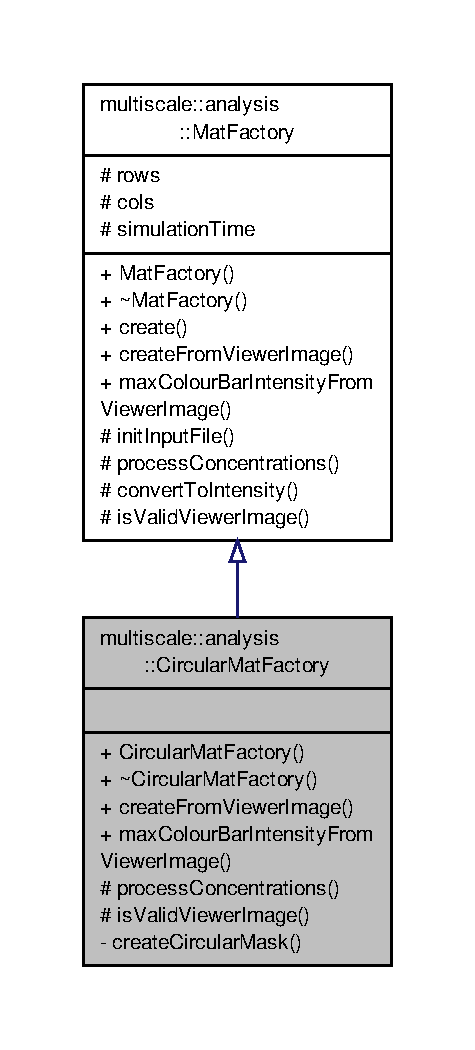
\includegraphics[height=550pt]{classmultiscale_1_1analysis_1_1CircularMatFactory__inherit__graph}
\end{center}
\end{figure}


Collaboration diagram for multiscale\-:\-:analysis\-:\-:Circular\-Mat\-Factory\-:\nopagebreak
\begin{figure}[H]
\begin{center}
\leavevmode
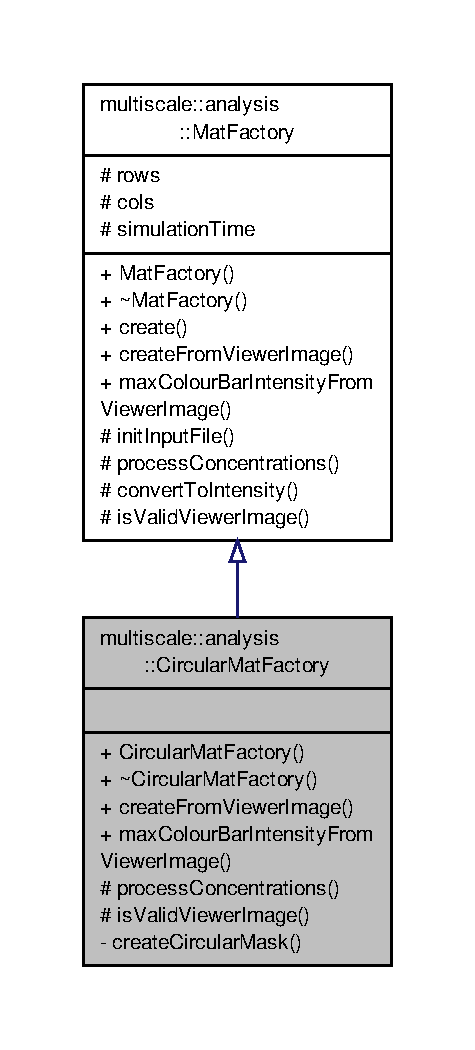
\includegraphics[height=550pt]{classmultiscale_1_1analysis_1_1CircularMatFactory__coll__graph}
\end{center}
\end{figure}
\subsection*{Public Member Functions}
\begin{DoxyCompactItemize}
\item 
\hyperlink{classmultiscale_1_1analysis_1_1CircularMatFactory_a9b4523850ed5fbf84f27d10a93a48f80}{Circular\-Mat\-Factory} ()
\item 
\hyperlink{classmultiscale_1_1analysis_1_1CircularMatFactory_aaf49d7ad7e1955709929d180686e99d8}{$\sim$\-Circular\-Mat\-Factory} ()
\item 
Mat \hyperlink{classmultiscale_1_1analysis_1_1CircularMatFactory_a8d5fccf946065b982bfa700b9e47b1f5}{create\-From\-Viewer\-Image} (const string \&input\-File) override
\begin{DoxyCompactList}\small\item\em Create a Mat object from the image file obtained from the Circular\-Geometry\-Viewer. \end{DoxyCompactList}\item 
double \hyperlink{classmultiscale_1_1analysis_1_1CircularMatFactory_aea41720f6adfb983bb94ea0a45789874}{max\-Colour\-Bar\-Intensity\-From\-Viewer\-Image} (const string \&input\-File) override
\begin{DoxyCompactList}\small\item\em Get the maximum grayscale intensity of the colour bar in the image. \end{DoxyCompactList}\end{DoxyCompactItemize}
\subsection*{Protected Member Functions}
\begin{DoxyCompactItemize}
\item 
unsigned char $\ast$ \hyperlink{classmultiscale_1_1analysis_1_1CircularMatFactory_a8fe40d38b896f440e17b5514462d1e8a}{process\-Concentrations} (ifstream \&fin) override
\begin{DoxyCompactList}\small\item\em Process the concentrations from the input file. \end{DoxyCompactList}\item 
bool \hyperlink{classmultiscale_1_1analysis_1_1CircularMatFactory_a08e407b35a2d314c1aa17f21040ff23a}{is\-Valid\-Viewer\-Image} (const Mat \&image) override
\begin{DoxyCompactList}\small\item\em Check if the image generated by the viewer has the required resolution. \end{DoxyCompactList}\end{DoxyCompactItemize}
\subsection*{Private Member Functions}
\begin{DoxyCompactItemize}
\item 
Mat \hyperlink{classmultiscale_1_1analysis_1_1CircularMatFactory_a94f2562c9045f2373b3e2736608de8c7}{create\-Circular\-Mask} (unsigned int origin\-X, unsigned int origin\-Y, unsigned int radius, const Mat \&image)
\begin{DoxyCompactList}\small\item\em Create a mask with 255 intensity pixels inside the circle with origin at (origin\-X, origin\-Y) and the given radius. \end{DoxyCompactList}\end{DoxyCompactItemize}
\subsection*{Static Private Attributes}
\begin{DoxyCompactItemize}
\item 
static const string \hyperlink{classmultiscale_1_1analysis_1_1CircularMatFactory_a7f4120aa31ff324ddb5c90e14cfeeb6d}{E\-R\-R\-\_\-\-U\-N\-I\-M\-P\-L\-E\-M\-E\-N\-T\-E\-D\-\_\-\-M\-E\-T\-H\-O\-D} = \char`\"{}The method you called is not implemented.\char`\"{}
\item 
static const int \hyperlink{classmultiscale_1_1analysis_1_1CircularMatFactory_a37f5cabf6d03d157cf96fb745e1da0ca}{I\-N\-T\-E\-N\-S\-I\-T\-Y\-\_\-\-M\-A\-X} = 255
\item 
static const int \hyperlink{classmultiscale_1_1analysis_1_1CircularMatFactory_a0e2da07df4736b0ec21567721ae94af5}{R\-O\-I\-\_\-\-S\-T\-A\-R\-T\-\_\-\-X} = 1024
\item 
static const int \hyperlink{classmultiscale_1_1analysis_1_1CircularMatFactory_a94368fde6348afd7074491c2cf333910}{R\-O\-I\-\_\-\-S\-T\-A\-R\-T\-\_\-\-Y} = 786
\item 
static const int \hyperlink{classmultiscale_1_1analysis_1_1CircularMatFactory_af26e9372a9bfb4428e9bdef952afedff}{R\-O\-I\-\_\-\-R\-A\-D\-I\-U\-S} = 615
\item 
static const int \hyperlink{classmultiscale_1_1analysis_1_1CircularMatFactory_a1c85fef366f2b3674a0c58394e441908}{I\-N\-P\-U\-T\-\_\-\-I\-M\-G\-\_\-\-W\-I\-D\-T\-H} = 2048
\item 
static const int \hyperlink{classmultiscale_1_1analysis_1_1CircularMatFactory_afdc7e6c3051b6767fa9e1a38257f1aa2}{I\-N\-P\-U\-T\-\_\-\-I\-M\-G\-\_\-\-H\-E\-I\-G\-H\-T} = 1572
\item 
static const int \hyperlink{classmultiscale_1_1analysis_1_1CircularMatFactory_a57e022b6cb2066b59e6f1988986ce6ad}{C\-O\-L\-O\-U\-R\-B\-A\-R\-\_\-\-M\-A\-X\-\_\-\-X} = 1775
\item 
static const int \hyperlink{classmultiscale_1_1analysis_1_1CircularMatFactory_a288197056f07989be0503e08a2745bed}{C\-O\-L\-O\-U\-R\-B\-A\-R\-\_\-\-M\-A\-X\-\_\-\-Y} = 56
\end{DoxyCompactItemize}
\subsection*{Additional Inherited Members}


\subsection{Detailed Description}
Class for creating a Mat object considering a circular grid. 

Definition at line 15 of file Circular\-Mat\-Factory.\-hpp.



\subsection{Constructor \& Destructor Documentation}
\hypertarget{classmultiscale_1_1analysis_1_1CircularMatFactory_a9b4523850ed5fbf84f27d10a93a48f80}{\index{multiscale\-::analysis\-::\-Circular\-Mat\-Factory@{multiscale\-::analysis\-::\-Circular\-Mat\-Factory}!Circular\-Mat\-Factory@{Circular\-Mat\-Factory}}
\index{Circular\-Mat\-Factory@{Circular\-Mat\-Factory}!multiscale::analysis::CircularMatFactory@{multiscale\-::analysis\-::\-Circular\-Mat\-Factory}}
\subsubsection[{Circular\-Mat\-Factory}]{\setlength{\rightskip}{0pt plus 5cm}Circular\-Mat\-Factory\-::\-Circular\-Mat\-Factory (
\begin{DoxyParamCaption}
{}
\end{DoxyParamCaption}
)}}\label{classmultiscale_1_1analysis_1_1CircularMatFactory_a9b4523850ed5fbf84f27d10a93a48f80}


Definition at line 9 of file Circular\-Mat\-Factory.\-cpp.

\hypertarget{classmultiscale_1_1analysis_1_1CircularMatFactory_aaf49d7ad7e1955709929d180686e99d8}{\index{multiscale\-::analysis\-::\-Circular\-Mat\-Factory@{multiscale\-::analysis\-::\-Circular\-Mat\-Factory}!$\sim$\-Circular\-Mat\-Factory@{$\sim$\-Circular\-Mat\-Factory}}
\index{$\sim$\-Circular\-Mat\-Factory@{$\sim$\-Circular\-Mat\-Factory}!multiscale::analysis::CircularMatFactory@{multiscale\-::analysis\-::\-Circular\-Mat\-Factory}}
\subsubsection[{$\sim$\-Circular\-Mat\-Factory}]{\setlength{\rightskip}{0pt plus 5cm}Circular\-Mat\-Factory\-::$\sim$\-Circular\-Mat\-Factory (
\begin{DoxyParamCaption}
{}
\end{DoxyParamCaption}
)}}\label{classmultiscale_1_1analysis_1_1CircularMatFactory_aaf49d7ad7e1955709929d180686e99d8}


Definition at line 11 of file Circular\-Mat\-Factory.\-cpp.



\subsection{Member Function Documentation}
\hypertarget{classmultiscale_1_1analysis_1_1CircularMatFactory_a94f2562c9045f2373b3e2736608de8c7}{\index{multiscale\-::analysis\-::\-Circular\-Mat\-Factory@{multiscale\-::analysis\-::\-Circular\-Mat\-Factory}!create\-Circular\-Mask@{create\-Circular\-Mask}}
\index{create\-Circular\-Mask@{create\-Circular\-Mask}!multiscale::analysis::CircularMatFactory@{multiscale\-::analysis\-::\-Circular\-Mat\-Factory}}
\subsubsection[{create\-Circular\-Mask}]{\setlength{\rightskip}{0pt plus 5cm}Mat Circular\-Mat\-Factory\-::create\-Circular\-Mask (
\begin{DoxyParamCaption}
\item[{unsigned int}]{origin\-X, }
\item[{unsigned int}]{origin\-Y, }
\item[{unsigned int}]{radius, }
\item[{const Mat \&}]{image}
\end{DoxyParamCaption}
)\hspace{0.3cm}{\ttfamily [private]}}}\label{classmultiscale_1_1analysis_1_1CircularMatFactory_a94f2562c9045f2373b3e2736608de8c7}


Create a mask with 255 intensity pixels inside the circle with origin at (origin\-X, origin\-Y) and the given radius. 

All the other pixels have intensity zero.

The original image is provided only for getting the size correctly


\begin{DoxyParams}{Parameters}
{\em origin\-X} & The x coordinate for the origin \\
\hline
{\em origin\-Y} & The y coordinate for the origin \\
\hline
{\em radius} & The size of the radius \\
\hline
{\em image} & The original image \\
\hline
\end{DoxyParams}


Definition at line 47 of file Circular\-Mat\-Factory.\-cpp.



References I\-N\-T\-E\-N\-S\-I\-T\-Y\-\_\-\-M\-A\-X.



Referenced by create\-From\-Viewer\-Image().



Here is the caller graph for this function\-:
\nopagebreak
\begin{figure}[H]
\begin{center}
\leavevmode
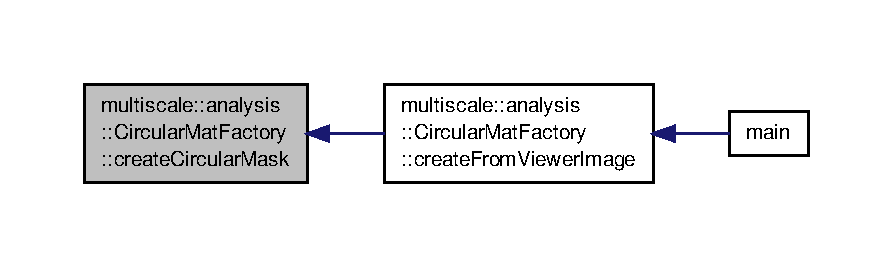
\includegraphics[width=350pt]{classmultiscale_1_1analysis_1_1CircularMatFactory_a94f2562c9045f2373b3e2736608de8c7_icgraph}
\end{center}
\end{figure}


\hypertarget{classmultiscale_1_1analysis_1_1CircularMatFactory_a8d5fccf946065b982bfa700b9e47b1f5}{\index{multiscale\-::analysis\-::\-Circular\-Mat\-Factory@{multiscale\-::analysis\-::\-Circular\-Mat\-Factory}!create\-From\-Viewer\-Image@{create\-From\-Viewer\-Image}}
\index{create\-From\-Viewer\-Image@{create\-From\-Viewer\-Image}!multiscale::analysis::CircularMatFactory@{multiscale\-::analysis\-::\-Circular\-Mat\-Factory}}
\subsubsection[{create\-From\-Viewer\-Image}]{\setlength{\rightskip}{0pt plus 5cm}Mat Circular\-Mat\-Factory\-::create\-From\-Viewer\-Image (
\begin{DoxyParamCaption}
\item[{const string \&}]{input\-File}
\end{DoxyParamCaption}
)\hspace{0.3cm}{\ttfamily [override]}, {\ttfamily [virtual]}}}\label{classmultiscale_1_1analysis_1_1CircularMatFactory_a8d5fccf946065b982bfa700b9e47b1f5}


Create a Mat object from the image file obtained from the Circular\-Geometry\-Viewer. 

Create the Mat instance from the given image file


\begin{DoxyParams}{Parameters}
{\em input\-File} & The path to the image file \\
\hline
\end{DoxyParams}


Implements \hyperlink{classmultiscale_1_1analysis_1_1MatFactory_a719ca9ac925ee182c1d5df1b0b029394}{multiscale\-::analysis\-::\-Mat\-Factory}.



Definition at line 13 of file Circular\-Mat\-Factory.\-cpp.



References create\-Circular\-Mask(), is\-Valid\-Viewer\-Image(), R\-O\-I\-\_\-\-R\-A\-D\-I\-U\-S, R\-O\-I\-\_\-\-S\-T\-A\-R\-T\-\_\-\-X, and R\-O\-I\-\_\-\-S\-T\-A\-R\-T\-\_\-\-Y.



Referenced by main().



Here is the call graph for this function\-:\nopagebreak
\begin{figure}[H]
\begin{center}
\leavevmode
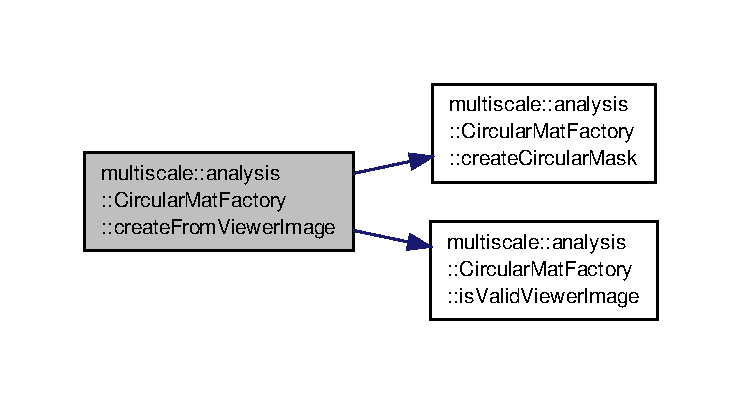
\includegraphics[width=350pt]{classmultiscale_1_1analysis_1_1CircularMatFactory_a8d5fccf946065b982bfa700b9e47b1f5_cgraph}
\end{center}
\end{figure}




Here is the caller graph for this function\-:
\nopagebreak
\begin{figure}[H]
\begin{center}
\leavevmode
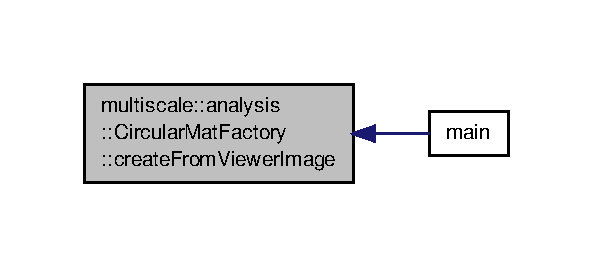
\includegraphics[width=284pt]{classmultiscale_1_1analysis_1_1CircularMatFactory_a8d5fccf946065b982bfa700b9e47b1f5_icgraph}
\end{center}
\end{figure}


\hypertarget{classmultiscale_1_1analysis_1_1CircularMatFactory_a08e407b35a2d314c1aa17f21040ff23a}{\index{multiscale\-::analysis\-::\-Circular\-Mat\-Factory@{multiscale\-::analysis\-::\-Circular\-Mat\-Factory}!is\-Valid\-Viewer\-Image@{is\-Valid\-Viewer\-Image}}
\index{is\-Valid\-Viewer\-Image@{is\-Valid\-Viewer\-Image}!multiscale::analysis::CircularMatFactory@{multiscale\-::analysis\-::\-Circular\-Mat\-Factory}}
\subsubsection[{is\-Valid\-Viewer\-Image}]{\setlength{\rightskip}{0pt plus 5cm}bool Circular\-Mat\-Factory\-::is\-Valid\-Viewer\-Image (
\begin{DoxyParamCaption}
\item[{const Mat \&}]{image}
\end{DoxyParamCaption}
)\hspace{0.3cm}{\ttfamily [override]}, {\ttfamily [protected]}, {\ttfamily [virtual]}}}\label{classmultiscale_1_1analysis_1_1CircularMatFactory_a08e407b35a2d314c1aa17f21040ff23a}


Check if the image generated by the viewer has the required resolution. 


\begin{DoxyParams}{Parameters}
{\em image} & Image generated by the viewer \\
\hline
\end{DoxyParams}


Implements \hyperlink{classmultiscale_1_1analysis_1_1MatFactory_ad6acdd120b128eb9fb502fca23a7de69}{multiscale\-::analysis\-::\-Mat\-Factory}.



Definition at line 56 of file Circular\-Mat\-Factory.\-cpp.



References multiscale\-::analysis\-::\-Mat\-Factory\-::\-E\-R\-R\-\_\-\-I\-M\-G\-\_\-\-R\-E\-S\-O\-L\-U\-T\-I\-O\-N, multiscale\-::analysis\-::\-Mat\-Factory\-::\-E\-R\-R\-\_\-\-I\-N\-P\-U\-T\-\_\-\-O\-P\-E\-N, I\-N\-P\-U\-T\-\_\-\-I\-M\-G\-\_\-\-H\-E\-I\-G\-H\-T, I\-N\-P\-U\-T\-\_\-\-I\-M\-G\-\_\-\-W\-I\-D\-T\-H, and M\-S\-\_\-throw.



Referenced by create\-From\-Viewer\-Image(), and max\-Colour\-Bar\-Intensity\-From\-Viewer\-Image().



Here is the caller graph for this function\-:
\nopagebreak
\begin{figure}[H]
\begin{center}
\leavevmode
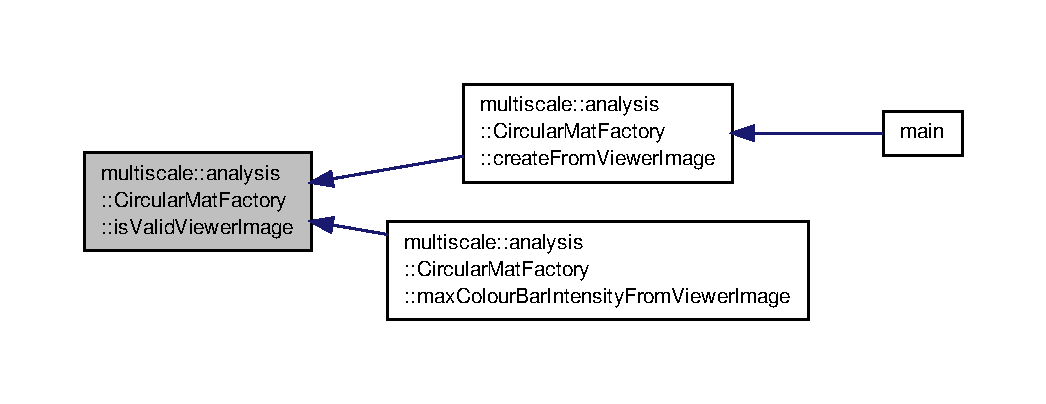
\includegraphics[width=350pt]{classmultiscale_1_1analysis_1_1CircularMatFactory_a08e407b35a2d314c1aa17f21040ff23a_icgraph}
\end{center}
\end{figure}


\hypertarget{classmultiscale_1_1analysis_1_1CircularMatFactory_aea41720f6adfb983bb94ea0a45789874}{\index{multiscale\-::analysis\-::\-Circular\-Mat\-Factory@{multiscale\-::analysis\-::\-Circular\-Mat\-Factory}!max\-Colour\-Bar\-Intensity\-From\-Viewer\-Image@{max\-Colour\-Bar\-Intensity\-From\-Viewer\-Image}}
\index{max\-Colour\-Bar\-Intensity\-From\-Viewer\-Image@{max\-Colour\-Bar\-Intensity\-From\-Viewer\-Image}!multiscale::analysis::CircularMatFactory@{multiscale\-::analysis\-::\-Circular\-Mat\-Factory}}
\subsubsection[{max\-Colour\-Bar\-Intensity\-From\-Viewer\-Image}]{\setlength{\rightskip}{0pt plus 5cm}double Circular\-Mat\-Factory\-::max\-Colour\-Bar\-Intensity\-From\-Viewer\-Image (
\begin{DoxyParamCaption}
\item[{const string \&}]{input\-File}
\end{DoxyParamCaption}
)\hspace{0.3cm}{\ttfamily [override]}, {\ttfamily [virtual]}}}\label{classmultiscale_1_1analysis_1_1CircularMatFactory_aea41720f6adfb983bb94ea0a45789874}


Get the maximum grayscale intensity of the colour bar in the image. 


\begin{DoxyParams}{Parameters}
{\em input\-File} & The path to the image file \\
\hline
\end{DoxyParams}


Implements \hyperlink{classmultiscale_1_1analysis_1_1MatFactory_a041b354357794476a2108e3f71deadc8}{multiscale\-::analysis\-::\-Mat\-Factory}.



Definition at line 32 of file Circular\-Mat\-Factory.\-cpp.



References C\-O\-L\-O\-U\-R\-B\-A\-R\-\_\-\-M\-A\-X\-\_\-\-X, C\-O\-L\-O\-U\-R\-B\-A\-R\-\_\-\-M\-A\-X\-\_\-\-Y, and is\-Valid\-Viewer\-Image().



Referenced by main().



Here is the call graph for this function\-:\nopagebreak
\begin{figure}[H]
\begin{center}
\leavevmode
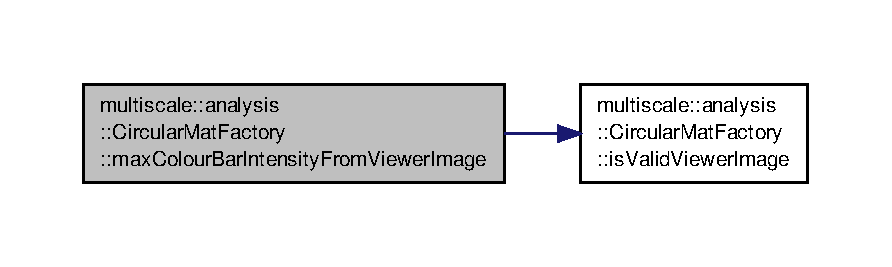
\includegraphics[width=350pt]{classmultiscale_1_1analysis_1_1CircularMatFactory_aea41720f6adfb983bb94ea0a45789874_cgraph}
\end{center}
\end{figure}




Here is the caller graph for this function\-:
\nopagebreak
\begin{figure}[H]
\begin{center}
\leavevmode
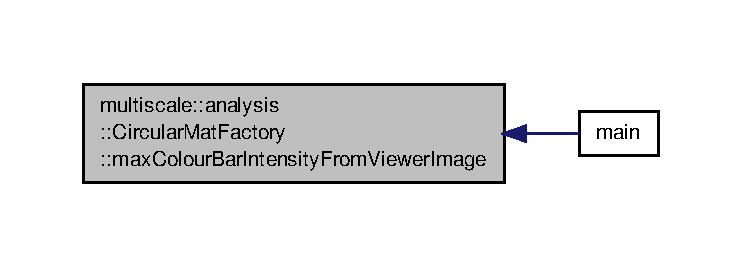
\includegraphics[width=350pt]{classmultiscale_1_1analysis_1_1CircularMatFactory_aea41720f6adfb983bb94ea0a45789874_icgraph}
\end{center}
\end{figure}


\hypertarget{classmultiscale_1_1analysis_1_1CircularMatFactory_a8fe40d38b896f440e17b5514462d1e8a}{\index{multiscale\-::analysis\-::\-Circular\-Mat\-Factory@{multiscale\-::analysis\-::\-Circular\-Mat\-Factory}!process\-Concentrations@{process\-Concentrations}}
\index{process\-Concentrations@{process\-Concentrations}!multiscale::analysis::CircularMatFactory@{multiscale\-::analysis\-::\-Circular\-Mat\-Factory}}
\subsubsection[{process\-Concentrations}]{\setlength{\rightskip}{0pt plus 5cm}unsigned char $\ast$ Circular\-Mat\-Factory\-::process\-Concentrations (
\begin{DoxyParamCaption}
\item[{ifstream \&}]{fin}
\end{DoxyParamCaption}
)\hspace{0.3cm}{\ttfamily [override]}, {\ttfamily [protected]}, {\ttfamily [virtual]}}}\label{classmultiscale_1_1analysis_1_1CircularMatFactory_a8fe40d38b896f440e17b5514462d1e8a}


Process the concentrations from the input file. 

R\-E\-M\-A\-R\-K\-: This method is not implemented and throws an error when called.


\begin{DoxyParams}{Parameters}
{\em fin} & Input file stream from which the concentrations are read \\
\hline
\end{DoxyParams}


Implements \hyperlink{classmultiscale_1_1analysis_1_1MatFactory_a0493c87d7b74619a95f14c0e31a3e178}{multiscale\-::analysis\-::\-Mat\-Factory}.



Definition at line 40 of file Circular\-Mat\-Factory.\-cpp.



References E\-R\-R\-\_\-\-U\-N\-I\-M\-P\-L\-E\-M\-E\-N\-T\-E\-D\-\_\-\-M\-E\-T\-H\-O\-D, and M\-S\-\_\-throw.



\subsection{Member Data Documentation}
\hypertarget{classmultiscale_1_1analysis_1_1CircularMatFactory_a57e022b6cb2066b59e6f1988986ce6ad}{\index{multiscale\-::analysis\-::\-Circular\-Mat\-Factory@{multiscale\-::analysis\-::\-Circular\-Mat\-Factory}!C\-O\-L\-O\-U\-R\-B\-A\-R\-\_\-\-M\-A\-X\-\_\-\-X@{C\-O\-L\-O\-U\-R\-B\-A\-R\-\_\-\-M\-A\-X\-\_\-\-X}}
\index{C\-O\-L\-O\-U\-R\-B\-A\-R\-\_\-\-M\-A\-X\-\_\-\-X@{C\-O\-L\-O\-U\-R\-B\-A\-R\-\_\-\-M\-A\-X\-\_\-\-X}!multiscale::analysis::CircularMatFactory@{multiscale\-::analysis\-::\-Circular\-Mat\-Factory}}
\subsubsection[{C\-O\-L\-O\-U\-R\-B\-A\-R\-\_\-\-M\-A\-X\-\_\-\-X}]{\setlength{\rightskip}{0pt plus 5cm}const int Circular\-Mat\-Factory\-::\-C\-O\-L\-O\-U\-R\-B\-A\-R\-\_\-\-M\-A\-X\-\_\-\-X = 1775\hspace{0.3cm}{\ttfamily [static]}, {\ttfamily [private]}}}\label{classmultiscale_1_1analysis_1_1CircularMatFactory_a57e022b6cb2066b59e6f1988986ce6ad}


Definition at line 82 of file Circular\-Mat\-Factory.\-hpp.



Referenced by max\-Colour\-Bar\-Intensity\-From\-Viewer\-Image().

\hypertarget{classmultiscale_1_1analysis_1_1CircularMatFactory_a288197056f07989be0503e08a2745bed}{\index{multiscale\-::analysis\-::\-Circular\-Mat\-Factory@{multiscale\-::analysis\-::\-Circular\-Mat\-Factory}!C\-O\-L\-O\-U\-R\-B\-A\-R\-\_\-\-M\-A\-X\-\_\-\-Y@{C\-O\-L\-O\-U\-R\-B\-A\-R\-\_\-\-M\-A\-X\-\_\-\-Y}}
\index{C\-O\-L\-O\-U\-R\-B\-A\-R\-\_\-\-M\-A\-X\-\_\-\-Y@{C\-O\-L\-O\-U\-R\-B\-A\-R\-\_\-\-M\-A\-X\-\_\-\-Y}!multiscale::analysis::CircularMatFactory@{multiscale\-::analysis\-::\-Circular\-Mat\-Factory}}
\subsubsection[{C\-O\-L\-O\-U\-R\-B\-A\-R\-\_\-\-M\-A\-X\-\_\-\-Y}]{\setlength{\rightskip}{0pt plus 5cm}const int Circular\-Mat\-Factory\-::\-C\-O\-L\-O\-U\-R\-B\-A\-R\-\_\-\-M\-A\-X\-\_\-\-Y = 56\hspace{0.3cm}{\ttfamily [static]}, {\ttfamily [private]}}}\label{classmultiscale_1_1analysis_1_1CircularMatFactory_a288197056f07989be0503e08a2745bed}


Definition at line 83 of file Circular\-Mat\-Factory.\-hpp.



Referenced by max\-Colour\-Bar\-Intensity\-From\-Viewer\-Image().

\hypertarget{classmultiscale_1_1analysis_1_1CircularMatFactory_a7f4120aa31ff324ddb5c90e14cfeeb6d}{\index{multiscale\-::analysis\-::\-Circular\-Mat\-Factory@{multiscale\-::analysis\-::\-Circular\-Mat\-Factory}!E\-R\-R\-\_\-\-U\-N\-I\-M\-P\-L\-E\-M\-E\-N\-T\-E\-D\-\_\-\-M\-E\-T\-H\-O\-D@{E\-R\-R\-\_\-\-U\-N\-I\-M\-P\-L\-E\-M\-E\-N\-T\-E\-D\-\_\-\-M\-E\-T\-H\-O\-D}}
\index{E\-R\-R\-\_\-\-U\-N\-I\-M\-P\-L\-E\-M\-E\-N\-T\-E\-D\-\_\-\-M\-E\-T\-H\-O\-D@{E\-R\-R\-\_\-\-U\-N\-I\-M\-P\-L\-E\-M\-E\-N\-T\-E\-D\-\_\-\-M\-E\-T\-H\-O\-D}!multiscale::analysis::CircularMatFactory@{multiscale\-::analysis\-::\-Circular\-Mat\-Factory}}
\subsubsection[{E\-R\-R\-\_\-\-U\-N\-I\-M\-P\-L\-E\-M\-E\-N\-T\-E\-D\-\_\-\-M\-E\-T\-H\-O\-D}]{\setlength{\rightskip}{0pt plus 5cm}const string Circular\-Mat\-Factory\-::\-E\-R\-R\-\_\-\-U\-N\-I\-M\-P\-L\-E\-M\-E\-N\-T\-E\-D\-\_\-\-M\-E\-T\-H\-O\-D = \char`\"{}The method you called is not implemented.\char`\"{}\hspace{0.3cm}{\ttfamily [static]}, {\ttfamily [private]}}}\label{classmultiscale_1_1analysis_1_1CircularMatFactory_a7f4120aa31ff324ddb5c90e14cfeeb6d}


Definition at line 71 of file Circular\-Mat\-Factory.\-hpp.



Referenced by process\-Concentrations().

\hypertarget{classmultiscale_1_1analysis_1_1CircularMatFactory_afdc7e6c3051b6767fa9e1a38257f1aa2}{\index{multiscale\-::analysis\-::\-Circular\-Mat\-Factory@{multiscale\-::analysis\-::\-Circular\-Mat\-Factory}!I\-N\-P\-U\-T\-\_\-\-I\-M\-G\-\_\-\-H\-E\-I\-G\-H\-T@{I\-N\-P\-U\-T\-\_\-\-I\-M\-G\-\_\-\-H\-E\-I\-G\-H\-T}}
\index{I\-N\-P\-U\-T\-\_\-\-I\-M\-G\-\_\-\-H\-E\-I\-G\-H\-T@{I\-N\-P\-U\-T\-\_\-\-I\-M\-G\-\_\-\-H\-E\-I\-G\-H\-T}!multiscale::analysis::CircularMatFactory@{multiscale\-::analysis\-::\-Circular\-Mat\-Factory}}
\subsubsection[{I\-N\-P\-U\-T\-\_\-\-I\-M\-G\-\_\-\-H\-E\-I\-G\-H\-T}]{\setlength{\rightskip}{0pt plus 5cm}const int Circular\-Mat\-Factory\-::\-I\-N\-P\-U\-T\-\_\-\-I\-M\-G\-\_\-\-H\-E\-I\-G\-H\-T = 1572\hspace{0.3cm}{\ttfamily [static]}, {\ttfamily [private]}}}\label{classmultiscale_1_1analysis_1_1CircularMatFactory_afdc7e6c3051b6767fa9e1a38257f1aa2}


Definition at line 80 of file Circular\-Mat\-Factory.\-hpp.



Referenced by is\-Valid\-Viewer\-Image().

\hypertarget{classmultiscale_1_1analysis_1_1CircularMatFactory_a1c85fef366f2b3674a0c58394e441908}{\index{multiscale\-::analysis\-::\-Circular\-Mat\-Factory@{multiscale\-::analysis\-::\-Circular\-Mat\-Factory}!I\-N\-P\-U\-T\-\_\-\-I\-M\-G\-\_\-\-W\-I\-D\-T\-H@{I\-N\-P\-U\-T\-\_\-\-I\-M\-G\-\_\-\-W\-I\-D\-T\-H}}
\index{I\-N\-P\-U\-T\-\_\-\-I\-M\-G\-\_\-\-W\-I\-D\-T\-H@{I\-N\-P\-U\-T\-\_\-\-I\-M\-G\-\_\-\-W\-I\-D\-T\-H}!multiscale::analysis::CircularMatFactory@{multiscale\-::analysis\-::\-Circular\-Mat\-Factory}}
\subsubsection[{I\-N\-P\-U\-T\-\_\-\-I\-M\-G\-\_\-\-W\-I\-D\-T\-H}]{\setlength{\rightskip}{0pt plus 5cm}const int Circular\-Mat\-Factory\-::\-I\-N\-P\-U\-T\-\_\-\-I\-M\-G\-\_\-\-W\-I\-D\-T\-H = 2048\hspace{0.3cm}{\ttfamily [static]}, {\ttfamily [private]}}}\label{classmultiscale_1_1analysis_1_1CircularMatFactory_a1c85fef366f2b3674a0c58394e441908}


Definition at line 79 of file Circular\-Mat\-Factory.\-hpp.



Referenced by is\-Valid\-Viewer\-Image().

\hypertarget{classmultiscale_1_1analysis_1_1CircularMatFactory_a37f5cabf6d03d157cf96fb745e1da0ca}{\index{multiscale\-::analysis\-::\-Circular\-Mat\-Factory@{multiscale\-::analysis\-::\-Circular\-Mat\-Factory}!I\-N\-T\-E\-N\-S\-I\-T\-Y\-\_\-\-M\-A\-X@{I\-N\-T\-E\-N\-S\-I\-T\-Y\-\_\-\-M\-A\-X}}
\index{I\-N\-T\-E\-N\-S\-I\-T\-Y\-\_\-\-M\-A\-X@{I\-N\-T\-E\-N\-S\-I\-T\-Y\-\_\-\-M\-A\-X}!multiscale::analysis::CircularMatFactory@{multiscale\-::analysis\-::\-Circular\-Mat\-Factory}}
\subsubsection[{I\-N\-T\-E\-N\-S\-I\-T\-Y\-\_\-\-M\-A\-X}]{\setlength{\rightskip}{0pt plus 5cm}const int Circular\-Mat\-Factory\-::\-I\-N\-T\-E\-N\-S\-I\-T\-Y\-\_\-\-M\-A\-X = 255\hspace{0.3cm}{\ttfamily [static]}, {\ttfamily [private]}}}\label{classmultiscale_1_1analysis_1_1CircularMatFactory_a37f5cabf6d03d157cf96fb745e1da0ca}


Definition at line 73 of file Circular\-Mat\-Factory.\-hpp.



Referenced by create\-Circular\-Mask().

\hypertarget{classmultiscale_1_1analysis_1_1CircularMatFactory_af26e9372a9bfb4428e9bdef952afedff}{\index{multiscale\-::analysis\-::\-Circular\-Mat\-Factory@{multiscale\-::analysis\-::\-Circular\-Mat\-Factory}!R\-O\-I\-\_\-\-R\-A\-D\-I\-U\-S@{R\-O\-I\-\_\-\-R\-A\-D\-I\-U\-S}}
\index{R\-O\-I\-\_\-\-R\-A\-D\-I\-U\-S@{R\-O\-I\-\_\-\-R\-A\-D\-I\-U\-S}!multiscale::analysis::CircularMatFactory@{multiscale\-::analysis\-::\-Circular\-Mat\-Factory}}
\subsubsection[{R\-O\-I\-\_\-\-R\-A\-D\-I\-U\-S}]{\setlength{\rightskip}{0pt plus 5cm}const int Circular\-Mat\-Factory\-::\-R\-O\-I\-\_\-\-R\-A\-D\-I\-U\-S = 615\hspace{0.3cm}{\ttfamily [static]}, {\ttfamily [private]}}}\label{classmultiscale_1_1analysis_1_1CircularMatFactory_af26e9372a9bfb4428e9bdef952afedff}


Definition at line 77 of file Circular\-Mat\-Factory.\-hpp.



Referenced by create\-From\-Viewer\-Image().

\hypertarget{classmultiscale_1_1analysis_1_1CircularMatFactory_a0e2da07df4736b0ec21567721ae94af5}{\index{multiscale\-::analysis\-::\-Circular\-Mat\-Factory@{multiscale\-::analysis\-::\-Circular\-Mat\-Factory}!R\-O\-I\-\_\-\-S\-T\-A\-R\-T\-\_\-\-X@{R\-O\-I\-\_\-\-S\-T\-A\-R\-T\-\_\-\-X}}
\index{R\-O\-I\-\_\-\-S\-T\-A\-R\-T\-\_\-\-X@{R\-O\-I\-\_\-\-S\-T\-A\-R\-T\-\_\-\-X}!multiscale::analysis::CircularMatFactory@{multiscale\-::analysis\-::\-Circular\-Mat\-Factory}}
\subsubsection[{R\-O\-I\-\_\-\-S\-T\-A\-R\-T\-\_\-\-X}]{\setlength{\rightskip}{0pt plus 5cm}const int Circular\-Mat\-Factory\-::\-R\-O\-I\-\_\-\-S\-T\-A\-R\-T\-\_\-\-X = 1024\hspace{0.3cm}{\ttfamily [static]}, {\ttfamily [private]}}}\label{classmultiscale_1_1analysis_1_1CircularMatFactory_a0e2da07df4736b0ec21567721ae94af5}


Definition at line 75 of file Circular\-Mat\-Factory.\-hpp.



Referenced by create\-From\-Viewer\-Image().

\hypertarget{classmultiscale_1_1analysis_1_1CircularMatFactory_a94368fde6348afd7074491c2cf333910}{\index{multiscale\-::analysis\-::\-Circular\-Mat\-Factory@{multiscale\-::analysis\-::\-Circular\-Mat\-Factory}!R\-O\-I\-\_\-\-S\-T\-A\-R\-T\-\_\-\-Y@{R\-O\-I\-\_\-\-S\-T\-A\-R\-T\-\_\-\-Y}}
\index{R\-O\-I\-\_\-\-S\-T\-A\-R\-T\-\_\-\-Y@{R\-O\-I\-\_\-\-S\-T\-A\-R\-T\-\_\-\-Y}!multiscale::analysis::CircularMatFactory@{multiscale\-::analysis\-::\-Circular\-Mat\-Factory}}
\subsubsection[{R\-O\-I\-\_\-\-S\-T\-A\-R\-T\-\_\-\-Y}]{\setlength{\rightskip}{0pt plus 5cm}const int Circular\-Mat\-Factory\-::\-R\-O\-I\-\_\-\-S\-T\-A\-R\-T\-\_\-\-Y = 786\hspace{0.3cm}{\ttfamily [static]}, {\ttfamily [private]}}}\label{classmultiscale_1_1analysis_1_1CircularMatFactory_a94368fde6348afd7074491c2cf333910}


Definition at line 76 of file Circular\-Mat\-Factory.\-hpp.



Referenced by create\-From\-Viewer\-Image().



The documentation for this class was generated from the following files\-:\begin{DoxyCompactItemize}
\item 
modules/analysis/spatial/include/multiscale/analysis/spatial/factory/\hyperlink{CircularMatFactory_8hpp}{Circular\-Mat\-Factory.\-hpp}\item 
modules/analysis/spatial/src/factory/\hyperlink{CircularMatFactory_8cpp}{Circular\-Mat\-Factory.\-cpp}\end{DoxyCompactItemize}

\hypertarget{classmultiscale_1_1CircularMatFactoryException}{\section{multiscale\-:\-:Circular\-Mat\-Factory\-Exception Class Reference}
\label{classmultiscale_1_1CircularMatFactoryException}\index{multiscale\-::\-Circular\-Mat\-Factory\-Exception@{multiscale\-::\-Circular\-Mat\-Factory\-Exception}}
}


Exception class for the Circular\-Mat\-Factory instances.  




{\ttfamily \#include $<$Circular\-Mat\-Factory\-Exception.\-hpp$>$}



Inheritance diagram for multiscale\-:\-:Circular\-Mat\-Factory\-Exception\-:
\nopagebreak
\begin{figure}[H]
\begin{center}
\leavevmode
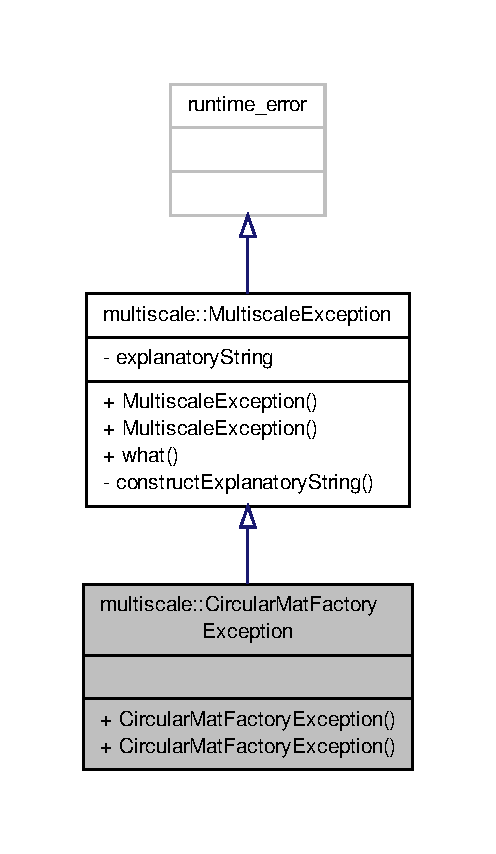
\includegraphics[width=238pt]{classmultiscale_1_1CircularMatFactoryException__inherit__graph}
\end{center}
\end{figure}


Collaboration diagram for multiscale\-:\-:Circular\-Mat\-Factory\-Exception\-:
\nopagebreak
\begin{figure}[H]
\begin{center}
\leavevmode
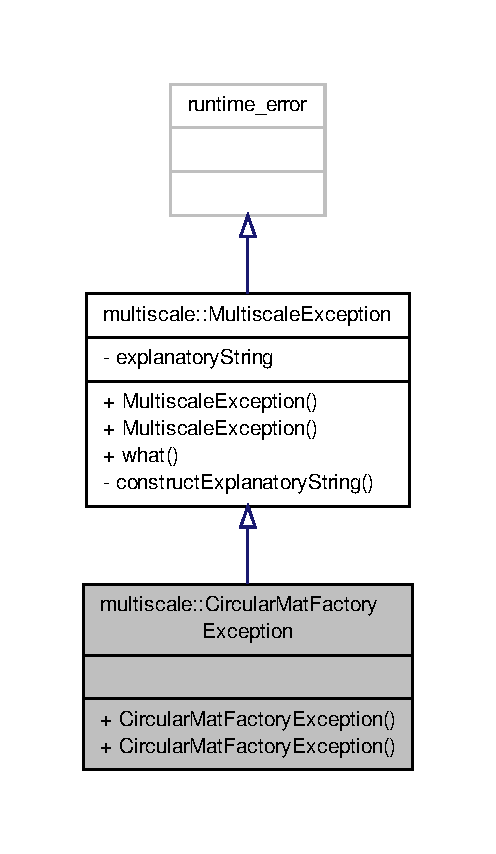
\includegraphics[width=238pt]{classmultiscale_1_1CircularMatFactoryException__coll__graph}
\end{center}
\end{figure}
\subsection*{Public Member Functions}
\begin{DoxyCompactItemize}
\item 
\hyperlink{classmultiscale_1_1CircularMatFactoryException_af9876b3e4dc7681bf52e03ac5375957a}{Circular\-Mat\-Factory\-Exception} (const string \&file, int line, const string \&msg)
\item 
\hyperlink{classmultiscale_1_1CircularMatFactoryException_a213e2ed3c46f995f9fa20e5ac73cfdf3}{Circular\-Mat\-Factory\-Exception} (const string \&file, int line, const char $\ast$msg)
\end{DoxyCompactItemize}


\subsection{Detailed Description}
Exception class for the Circular\-Mat\-Factory instances. 

Definition at line 14 of file Circular\-Mat\-Factory\-Exception.\-hpp.



\subsection{Constructor \& Destructor Documentation}
\hypertarget{classmultiscale_1_1CircularMatFactoryException_af9876b3e4dc7681bf52e03ac5375957a}{\index{multiscale\-::\-Circular\-Mat\-Factory\-Exception@{multiscale\-::\-Circular\-Mat\-Factory\-Exception}!Circular\-Mat\-Factory\-Exception@{Circular\-Mat\-Factory\-Exception}}
\index{Circular\-Mat\-Factory\-Exception@{Circular\-Mat\-Factory\-Exception}!multiscale::CircularMatFactoryException@{multiscale\-::\-Circular\-Mat\-Factory\-Exception}}
\subsubsection[{Circular\-Mat\-Factory\-Exception}]{\setlength{\rightskip}{0pt plus 5cm}multiscale\-::\-Circular\-Mat\-Factory\-Exception\-::\-Circular\-Mat\-Factory\-Exception (
\begin{DoxyParamCaption}
\item[{const string \&}]{file, }
\item[{int}]{line, }
\item[{const string \&}]{msg}
\end{DoxyParamCaption}
)\hspace{0.3cm}{\ttfamily [inline]}}}\label{classmultiscale_1_1CircularMatFactoryException_af9876b3e4dc7681bf52e03ac5375957a}


Definition at line 18 of file Circular\-Mat\-Factory\-Exception.\-hpp.

\hypertarget{classmultiscale_1_1CircularMatFactoryException_a213e2ed3c46f995f9fa20e5ac73cfdf3}{\index{multiscale\-::\-Circular\-Mat\-Factory\-Exception@{multiscale\-::\-Circular\-Mat\-Factory\-Exception}!Circular\-Mat\-Factory\-Exception@{Circular\-Mat\-Factory\-Exception}}
\index{Circular\-Mat\-Factory\-Exception@{Circular\-Mat\-Factory\-Exception}!multiscale::CircularMatFactoryException@{multiscale\-::\-Circular\-Mat\-Factory\-Exception}}
\subsubsection[{Circular\-Mat\-Factory\-Exception}]{\setlength{\rightskip}{0pt plus 5cm}multiscale\-::\-Circular\-Mat\-Factory\-Exception\-::\-Circular\-Mat\-Factory\-Exception (
\begin{DoxyParamCaption}
\item[{const string \&}]{file, }
\item[{int}]{line, }
\item[{const char $\ast$}]{msg}
\end{DoxyParamCaption}
)\hspace{0.3cm}{\ttfamily [inline]}}}\label{classmultiscale_1_1CircularMatFactoryException_a213e2ed3c46f995f9fa20e5ac73cfdf3}


Definition at line 20 of file Circular\-Mat\-Factory\-Exception.\-hpp.



The documentation for this class was generated from the following file\-:\begin{DoxyCompactItemize}
\item 
/home/ovidiu/\-Repositories/git/multiscale/\-Multiscale/include/multiscale/exception/\hyperlink{CircularMatFactoryException_8hpp}{Circular\-Mat\-Factory\-Exception.\-hpp}\end{DoxyCompactItemize}

\hypertarget{classmultiscale_1_1analysis_1_1Cluster}{\section{multiscale\-:\-:analysis\-:\-:Cluster Class Reference}
\label{classmultiscale_1_1analysis_1_1Cluster}\index{multiscale\-::analysis\-::\-Cluster@{multiscale\-::analysis\-::\-Cluster}}
}


Class for representing a cluster of entities in an image.  




{\ttfamily \#include $<$Cluster.\-hpp$>$}



Inheritance diagram for multiscale\-:\-:analysis\-:\-:Cluster\-:\nopagebreak
\begin{figure}[H]
\begin{center}
\leavevmode
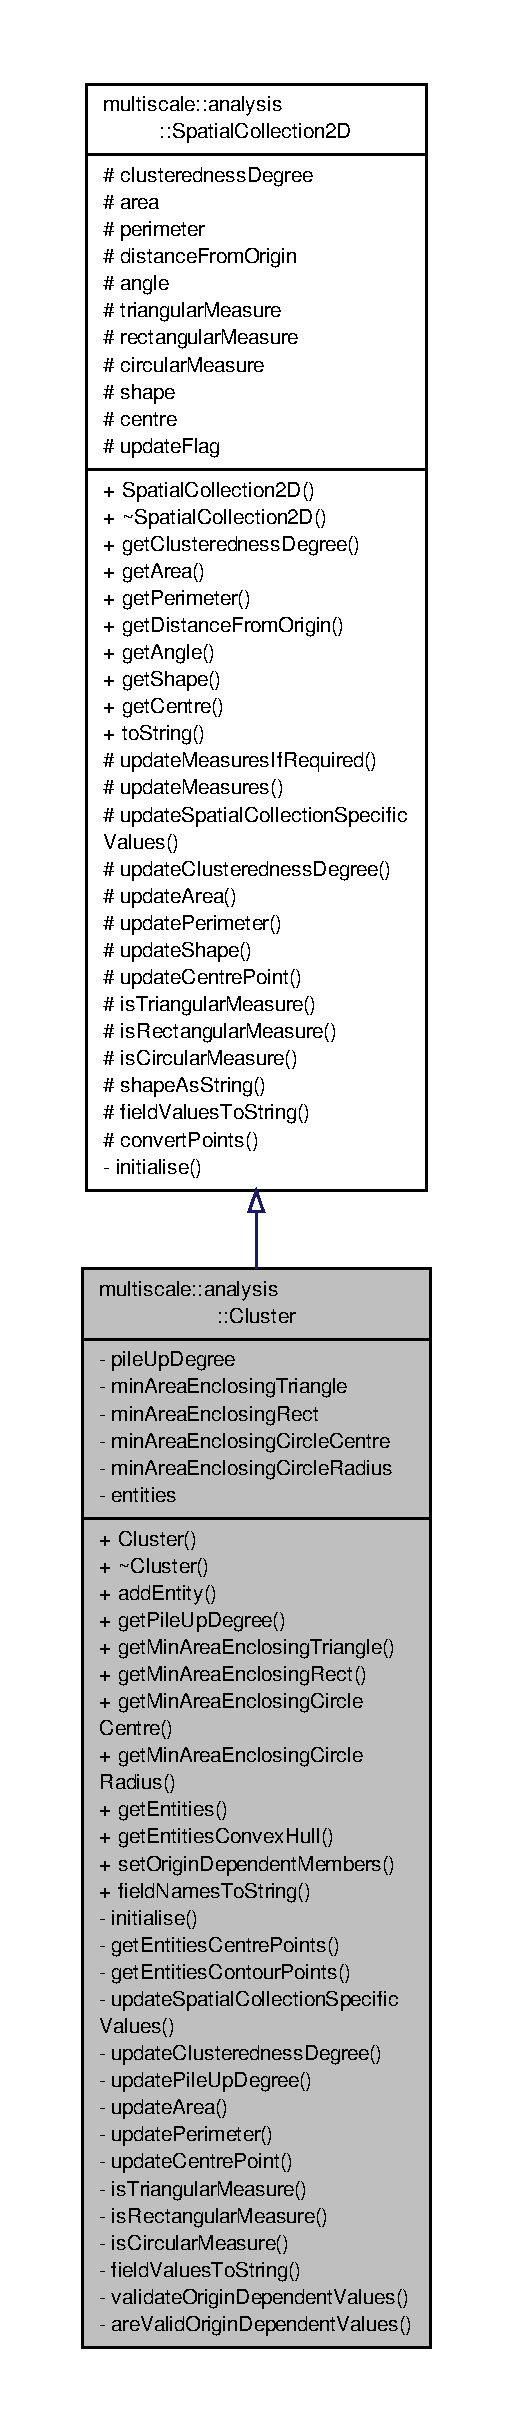
\includegraphics[height=550pt]{classmultiscale_1_1analysis_1_1Cluster__inherit__graph}
\end{center}
\end{figure}


Collaboration diagram for multiscale\-:\-:analysis\-:\-:Cluster\-:\nopagebreak
\begin{figure}[H]
\begin{center}
\leavevmode
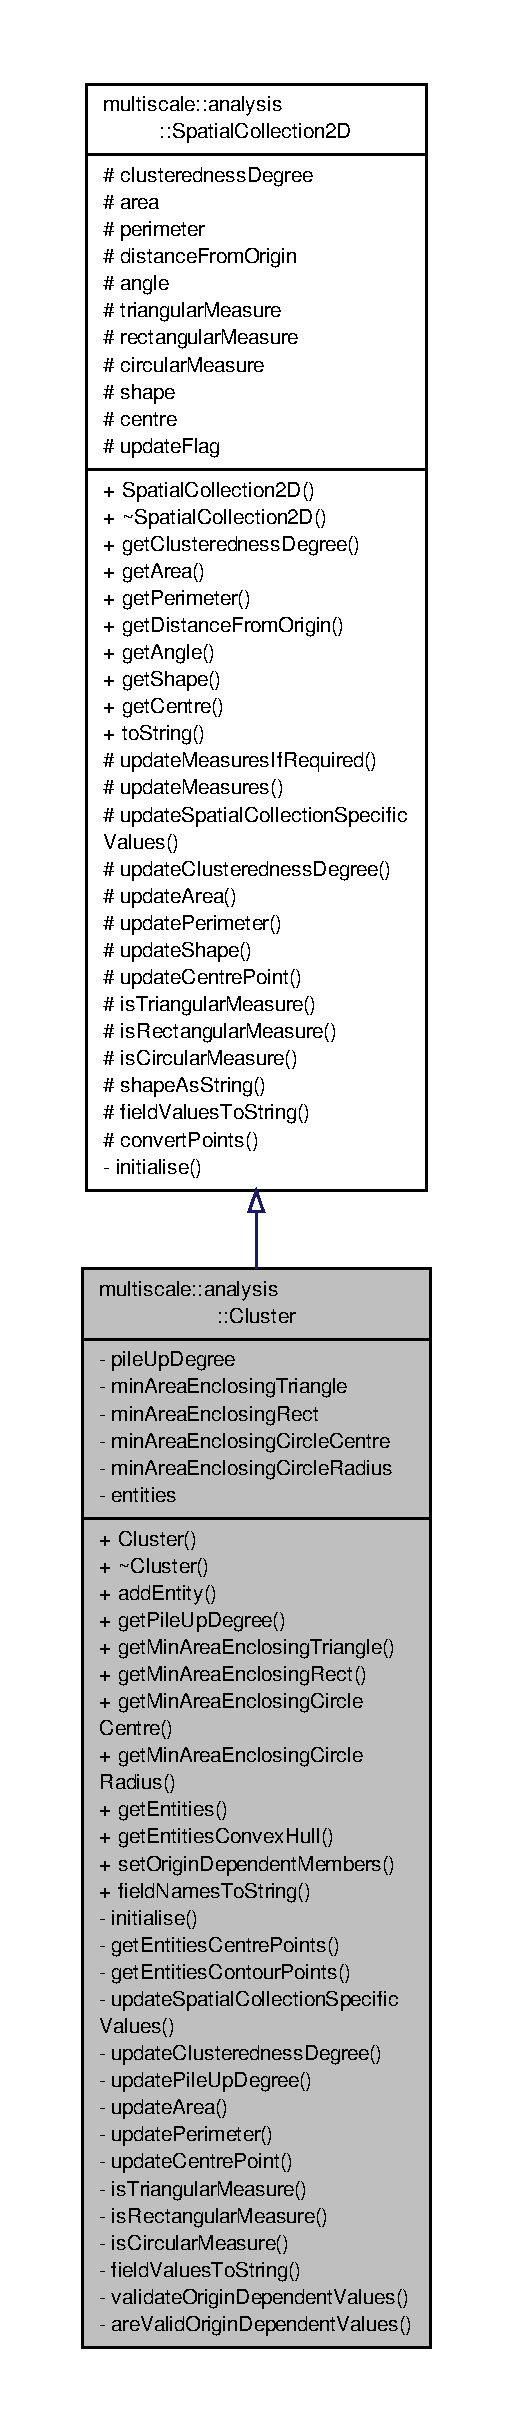
\includegraphics[height=550pt]{classmultiscale_1_1analysis_1_1Cluster__coll__graph}
\end{center}
\end{figure}
\subsection*{Public Member Functions}
\begin{DoxyCompactItemize}
\item 
\hyperlink{classmultiscale_1_1analysis_1_1Cluster_aee7feb1d599d4c8fda6c3ee83e86ba81}{Cluster} ()
\item 
\hyperlink{classmultiscale_1_1analysis_1_1Cluster_a4bddfc88ac859610acab15dd12851b58}{$\sim$\-Cluster} ()
\item 
void \hyperlink{classmultiscale_1_1analysis_1_1Cluster_a2bc85629ab2bd6d01c6d2df3d79ba497}{add\-Entity} (const \hyperlink{classmultiscale_1_1analysis_1_1Entity}{Entity} \&entity)
\begin{DoxyCompactList}\small\item\em Add a new entity to the cluster. \end{DoxyCompactList}\item 
vector$<$ Point2f $>$ \hyperlink{classmultiscale_1_1analysis_1_1Cluster_ab28150a739c35d66874c219fd38b462b}{get\-Min\-Area\-Enclosing\-Triangle} ()
\begin{DoxyCompactList}\small\item\em Get the minimum area enclosing triangle. \end{DoxyCompactList}\item 
Rotated\-Rect \hyperlink{classmultiscale_1_1analysis_1_1Cluster_a6417e3328622a848a7dedeebb5821750}{get\-Min\-Area\-Enclosing\-Rect} ()
\begin{DoxyCompactList}\small\item\em Get the minimum area enclosing rectangle. \end{DoxyCompactList}\item 
Point2f \hyperlink{classmultiscale_1_1analysis_1_1Cluster_a4d93f85faf929336818248e1fd604fb6}{get\-Min\-Area\-Enclosing\-Circle\-Centre} ()
\begin{DoxyCompactList}\small\item\em Get the minimum area enclosing circle centre. \end{DoxyCompactList}\item 
float \hyperlink{classmultiscale_1_1analysis_1_1Cluster_aecf5fa56fa21e3b22130242694be744f}{get\-Min\-Area\-Enclosing\-Circle\-Radius} ()
\begin{DoxyCompactList}\small\item\em Get the minimum area enclosing circle radius. \end{DoxyCompactList}\item 
vector$<$ \hyperlink{classmultiscale_1_1analysis_1_1Entity}{Entity} $>$ \hyperlink{classmultiscale_1_1analysis_1_1Cluster_aedd64d46ad3ea61ce7bb76be1f0906e6}{get\-Entities} () const 
\begin{DoxyCompactList}\small\item\em Get the collection of underlying entities. \end{DoxyCompactList}\item 
vector$<$ Point2f $>$ \hyperlink{classmultiscale_1_1analysis_1_1Cluster_a9f43161c58d9e4a97f3a33807397b255}{get\-Entities\-Convex\-Hull} ()
\begin{DoxyCompactList}\small\item\em Get the convex hull enclosing the collection of entities' contour points. \end{DoxyCompactList}\item 
void \hyperlink{classmultiscale_1_1analysis_1_1Cluster_a84033ee8d583d9195abbf42d5d420915}{set\-Origin\-Dependent\-Members} (double \hyperlink{classmultiscale_1_1analysis_1_1SpatialEntityPseudo3D_a056f67b90ed41c0e6dc4df31b71ad906}{distance\-From\-Origin}, double angle\-Wrt\-Origin)
\begin{DoxyCompactList}\small\item\em Set the values of the origin dependent members. \end{DoxyCompactList}\end{DoxyCompactItemize}
\subsection*{Static Public Attributes}
\begin{DoxyCompactItemize}
\item 
static const string \hyperlink{classmultiscale_1_1analysis_1_1Cluster_a546b8e93e3f1ef51a9932f8599639070}{E\-R\-R\-\_\-\-U\-N\-D\-E\-F\-I\-N\-E\-D\-\_\-\-S\-H\-A\-P\-E} = \char`\"{}The \hyperlink{classmultiscale_1_1analysis_1_1SpatialEntityPseudo3D_abad3acd3d7067e8e86e168e692cb2c2e}{shape} of the given cluster is undefined.\char`\"{}
\item 
static const string \hyperlink{classmultiscale_1_1analysis_1_1Cluster_a0fa38fcc3f00730409400578829cddd8}{E\-R\-R\-\_\-\-O\-R\-I\-G\-I\-N\-\_\-\-D\-E\-P\-E\-N\-D\-E\-N\-T\-\_\-\-V\-A\-L\-U\-E\-S} = \char`\"{}The origin dependent values are invalid (i.\-e. negative).\char`\"{}
\end{DoxyCompactItemize}
\subsection*{Private Member Functions}
\begin{DoxyCompactItemize}
\item 
void \hyperlink{classmultiscale_1_1analysis_1_1Cluster_a3af6980def4fbfea38ccd86620f127f8}{initialise} ()
\begin{DoxyCompactList}\small\item\em Initialisation function for the class. \end{DoxyCompactList}\item 
vector$<$ Point2f $>$ \hyperlink{classmultiscale_1_1analysis_1_1Cluster_af24261b08126bc2d2f51144056c6d353}{get\-Entities\-Centre\-Points} ()
\begin{DoxyCompactList}\small\item\em Get the collection of entities' centres. \end{DoxyCompactList}\item 
vector$<$ Point2f $>$ \hyperlink{classmultiscale_1_1analysis_1_1Cluster_adbb1a108b2ae638fbba0450c7f7fee20}{get\-Entities\-Contour\-Points} ()
\begin{DoxyCompactList}\small\item\em Get the collection of entities' contour points. \end{DoxyCompactList}\item 
void \hyperlink{classmultiscale_1_1analysis_1_1Cluster_a2279d1567eec7c0b1e29cae26cfb4d73}{update\-Clusteredness\-Degree} () override
\begin{DoxyCompactList}\small\item\em Update the value of the clusteredness degree. \end{DoxyCompactList}\item 
void \hyperlink{classmultiscale_1_1analysis_1_1Cluster_ac0300d9d05b0eb3aecd5724a14c2da41}{update\-Density} () override
\begin{DoxyCompactList}\small\item\em Update the value of the pile up degree. \end{DoxyCompactList}\item 
void \hyperlink{classmultiscale_1_1analysis_1_1Cluster_a3128a3b20c28619ccdd6a25208b8c83e}{update\-Area} () override
\begin{DoxyCompactList}\small\item\em Update the value of the area. \end{DoxyCompactList}\item 
void \hyperlink{classmultiscale_1_1analysis_1_1Cluster_aadc520e4459f1ea6e22afd7c02d5f2ed}{update\-Perimeter} () override
\begin{DoxyCompactList}\small\item\em Update the value of the perimeter. \end{DoxyCompactList}\item 
void \hyperlink{classmultiscale_1_1analysis_1_1Cluster_a1991d68cc9e76dab54c134df6beb59cb}{update\-Centre\-Point} () override
\begin{DoxyCompactList}\small\item\em Update the point defining the centre of the cluster. \end{DoxyCompactList}\item 
double \hyperlink{classmultiscale_1_1analysis_1_1Cluster_a28efcf050af76acb01619b36505b662e}{is\-Triangular\-Measure} () override
\begin{DoxyCompactList}\small\item\em Get the measure that the cluster has a triangular shape. \end{DoxyCompactList}\item 
double \hyperlink{classmultiscale_1_1analysis_1_1Cluster_aca93cb46704a3e824151e99b7a53d20d}{is\-Rectangular\-Measure} () override
\begin{DoxyCompactList}\small\item\em Get the measure that the cluster has a rectangular shape. \end{DoxyCompactList}\item 
double \hyperlink{classmultiscale_1_1analysis_1_1Cluster_a579730478055ae93d659f268375a492d}{is\-Circular\-Measure} () override
\begin{DoxyCompactList}\small\item\em Get the measure that the cluster has a circular shape. \end{DoxyCompactList}\item 
\hyperlink{namespacemultiscale_1_1analysis_a6db9cbf10615e77e300c3e4cb1c56660}{Spatial\-Entity\-Pseudo3\-D\-Type} \hyperlink{classmultiscale_1_1analysis_1_1Cluster_a0a4531d371662e9c4149c10aa115fb49}{type} () override
\begin{DoxyCompactList}\small\item\em Return the type of the pseudo 3\-D spatial entity. \end{DoxyCompactList}\item 
void \hyperlink{classmultiscale_1_1analysis_1_1Cluster_a26b9c11e63bfdbfc837a35f68c5c40dd}{validate\-Origin\-Dependent\-Values} (double \hyperlink{classmultiscale_1_1analysis_1_1SpatialEntityPseudo3D_a056f67b90ed41c0e6dc4df31b71ad906}{distance\-From\-Origin}, double angle\-Wrt\-Origin)
\begin{DoxyCompactList}\small\item\em Validate the origin dependent values (i.\-e. non-\/negative) \end{DoxyCompactList}\item 
bool \hyperlink{classmultiscale_1_1analysis_1_1Cluster_a05e8593354fabd5c1ca18b6a2b19096e}{are\-Valid\-Origin\-Dependent\-Values} (double \hyperlink{classmultiscale_1_1analysis_1_1SpatialEntityPseudo3D_a056f67b90ed41c0e6dc4df31b71ad906}{distance\-From\-Origin}, double angle\-Wrt\-Origin)
\begin{DoxyCompactList}\small\item\em Check if the origin dependent values are valid (i.\-e. non-\/negative) \end{DoxyCompactList}\end{DoxyCompactItemize}
\subsection*{Private Attributes}
\begin{DoxyCompactItemize}
\item 
vector$<$ Point2f $>$ \hyperlink{classmultiscale_1_1analysis_1_1Cluster_a7678d48581202c3ecc3f1283a1730dfa}{min\-Area\-Enclosing\-Triangle}
\item 
Rotated\-Rect \hyperlink{classmultiscale_1_1analysis_1_1Cluster_aeb032303a79c6bd43385fcaad9c50742}{min\-Area\-Enclosing\-Rect}
\item 
Point2f \hyperlink{classmultiscale_1_1analysis_1_1Cluster_a47e672060b4025dcd07ebb9c5fd99f0c}{min\-Area\-Enclosing\-Circle\-Centre}
\item 
float \hyperlink{classmultiscale_1_1analysis_1_1Cluster_a070994481884a4c7f5aa4879ce7b0568}{min\-Area\-Enclosing\-Circle\-Radius}
\item 
vector$<$ \hyperlink{classmultiscale_1_1analysis_1_1Entity}{Entity} $>$ \hyperlink{classmultiscale_1_1analysis_1_1Cluster_a820298479651328fb79d92a65f7923d6}{entities}
\end{DoxyCompactItemize}
\subsection*{Additional Inherited Members}


\subsection{Detailed Description}
Class for representing a cluster of entities in an image. 

Definition at line 21 of file Cluster.\-hpp.



\subsection{Constructor \& Destructor Documentation}
\hypertarget{classmultiscale_1_1analysis_1_1Cluster_aee7feb1d599d4c8fda6c3ee83e86ba81}{\index{multiscale\-::analysis\-::\-Cluster@{multiscale\-::analysis\-::\-Cluster}!Cluster@{Cluster}}
\index{Cluster@{Cluster}!multiscale::analysis::Cluster@{multiscale\-::analysis\-::\-Cluster}}
\subsubsection[{Cluster}]{\setlength{\rightskip}{0pt plus 5cm}Cluster\-::\-Cluster (
\begin{DoxyParamCaption}
{}
\end{DoxyParamCaption}
)}}\label{classmultiscale_1_1analysis_1_1Cluster_aee7feb1d599d4c8fda6c3ee83e86ba81}


Definition at line 11 of file Cluster.\-cpp.



References initialise().

\hypertarget{classmultiscale_1_1analysis_1_1Cluster_a4bddfc88ac859610acab15dd12851b58}{\index{multiscale\-::analysis\-::\-Cluster@{multiscale\-::analysis\-::\-Cluster}!$\sim$\-Cluster@{$\sim$\-Cluster}}
\index{$\sim$\-Cluster@{$\sim$\-Cluster}!multiscale::analysis::Cluster@{multiscale\-::analysis\-::\-Cluster}}
\subsubsection[{$\sim$\-Cluster}]{\setlength{\rightskip}{0pt plus 5cm}Cluster\-::$\sim$\-Cluster (
\begin{DoxyParamCaption}
{}
\end{DoxyParamCaption}
)}}\label{classmultiscale_1_1analysis_1_1Cluster_a4bddfc88ac859610acab15dd12851b58}


Definition at line 15 of file Cluster.\-cpp.



\subsection{Member Function Documentation}
\hypertarget{classmultiscale_1_1analysis_1_1Cluster_a2bc85629ab2bd6d01c6d2df3d79ba497}{\index{multiscale\-::analysis\-::\-Cluster@{multiscale\-::analysis\-::\-Cluster}!add\-Entity@{add\-Entity}}
\index{add\-Entity@{add\-Entity}!multiscale::analysis::Cluster@{multiscale\-::analysis\-::\-Cluster}}
\subsubsection[{add\-Entity}]{\setlength{\rightskip}{0pt plus 5cm}void Cluster\-::add\-Entity (
\begin{DoxyParamCaption}
\item[{const {\bf Entity} \&}]{entity}
\end{DoxyParamCaption}
)}}\label{classmultiscale_1_1analysis_1_1Cluster_a2bc85629ab2bd6d01c6d2df3d79ba497}


Add a new entity to the cluster. 



Definition at line 17 of file Cluster.\-cpp.



References entities, and multiscale\-::analysis\-::\-Spatial\-Entity\-Pseudo3\-D\-::update\-Flag.

\hypertarget{classmultiscale_1_1analysis_1_1Cluster_a05e8593354fabd5c1ca18b6a2b19096e}{\index{multiscale\-::analysis\-::\-Cluster@{multiscale\-::analysis\-::\-Cluster}!are\-Valid\-Origin\-Dependent\-Values@{are\-Valid\-Origin\-Dependent\-Values}}
\index{are\-Valid\-Origin\-Dependent\-Values@{are\-Valid\-Origin\-Dependent\-Values}!multiscale::analysis::Cluster@{multiscale\-::analysis\-::\-Cluster}}
\subsubsection[{are\-Valid\-Origin\-Dependent\-Values}]{\setlength{\rightskip}{0pt plus 5cm}bool Cluster\-::are\-Valid\-Origin\-Dependent\-Values (
\begin{DoxyParamCaption}
\item[{double}]{distance\-From\-Origin, }
\item[{double}]{angle\-Wrt\-Origin}
\end{DoxyParamCaption}
)\hspace{0.3cm}{\ttfamily [private]}}}\label{classmultiscale_1_1analysis_1_1Cluster_a05e8593354fabd5c1ca18b6a2b19096e}


Check if the origin dependent values are valid (i.\-e. non-\/negative) 


\begin{DoxyParams}{Parameters}
{\em distance\-From\-Origin} & Distance from the origin \\
\hline
{\em angle\-Wrt\-Origin} & Angle with respect to the origin \\
\hline
\end{DoxyParams}


Definition at line 199 of file Cluster.\-cpp.



References multiscale\-::\-Numeric\-::greater\-Or\-Equal().



Referenced by validate\-Origin\-Dependent\-Values().



Here is the caller graph for this function\-:\nopagebreak
\begin{figure}[H]
\begin{center}
\leavevmode
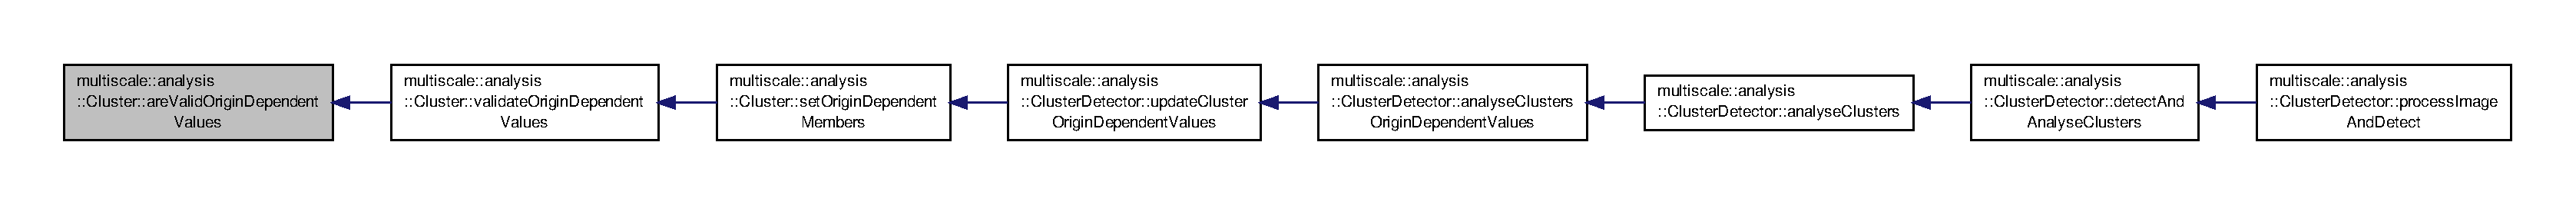
\includegraphics[width=350pt]{classmultiscale_1_1analysis_1_1Cluster_a05e8593354fabd5c1ca18b6a2b19096e_icgraph}
\end{center}
\end{figure}


\hypertarget{classmultiscale_1_1analysis_1_1Cluster_aedd64d46ad3ea61ce7bb76be1f0906e6}{\index{multiscale\-::analysis\-::\-Cluster@{multiscale\-::analysis\-::\-Cluster}!get\-Entities@{get\-Entities}}
\index{get\-Entities@{get\-Entities}!multiscale::analysis::Cluster@{multiscale\-::analysis\-::\-Cluster}}
\subsubsection[{get\-Entities}]{\setlength{\rightskip}{0pt plus 5cm}vector$<$ {\bf Entity} $>$ Cluster\-::get\-Entities (
\begin{DoxyParamCaption}
{}
\end{DoxyParamCaption}
) const}}\label{classmultiscale_1_1analysis_1_1Cluster_aedd64d46ad3ea61ce7bb76be1f0906e6}


Get the collection of underlying entities. 



Definition at line 47 of file Cluster.\-cpp.



References entities.



Referenced by multiscale\-::analysis\-::\-Simulation\-Cluster\-Detector\-::output\-Cluster\-To\-Image().



Here is the caller graph for this function\-:\nopagebreak
\begin{figure}[H]
\begin{center}
\leavevmode
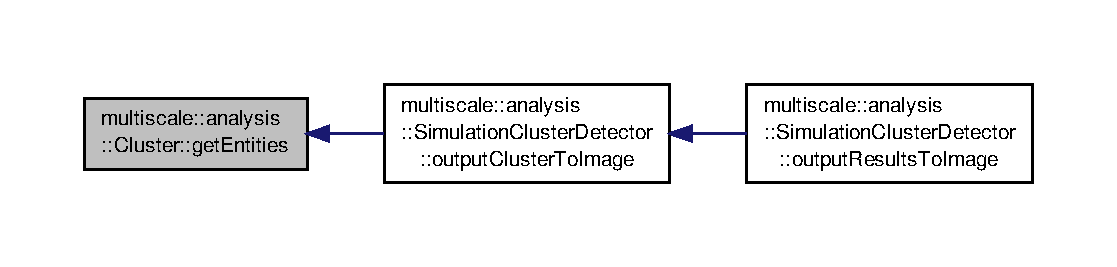
\includegraphics[width=350pt]{classmultiscale_1_1analysis_1_1Cluster_aedd64d46ad3ea61ce7bb76be1f0906e6_icgraph}
\end{center}
\end{figure}


\hypertarget{classmultiscale_1_1analysis_1_1Cluster_af24261b08126bc2d2f51144056c6d353}{\index{multiscale\-::analysis\-::\-Cluster@{multiscale\-::analysis\-::\-Cluster}!get\-Entities\-Centre\-Points@{get\-Entities\-Centre\-Points}}
\index{get\-Entities\-Centre\-Points@{get\-Entities\-Centre\-Points}!multiscale::analysis::Cluster@{multiscale\-::analysis\-::\-Cluster}}
\subsubsection[{get\-Entities\-Centre\-Points}]{\setlength{\rightskip}{0pt plus 5cm}vector$<$ Point2f $>$ Cluster\-::get\-Entities\-Centre\-Points (
\begin{DoxyParamCaption}
{}
\end{DoxyParamCaption}
)\hspace{0.3cm}{\ttfamily [private]}}}\label{classmultiscale_1_1analysis_1_1Cluster_af24261b08126bc2d2f51144056c6d353}


Get the collection of entities' centres. 



Definition at line 84 of file Cluster.\-cpp.



References entities.

\hypertarget{classmultiscale_1_1analysis_1_1Cluster_adbb1a108b2ae638fbba0450c7f7fee20}{\index{multiscale\-::analysis\-::\-Cluster@{multiscale\-::analysis\-::\-Cluster}!get\-Entities\-Contour\-Points@{get\-Entities\-Contour\-Points}}
\index{get\-Entities\-Contour\-Points@{get\-Entities\-Contour\-Points}!multiscale::analysis::Cluster@{multiscale\-::analysis\-::\-Cluster}}
\subsubsection[{get\-Entities\-Contour\-Points}]{\setlength{\rightskip}{0pt plus 5cm}vector$<$ Point2f $>$ Cluster\-::get\-Entities\-Contour\-Points (
\begin{DoxyParamCaption}
{}
\end{DoxyParamCaption}
)\hspace{0.3cm}{\ttfamily [private]}}}\label{classmultiscale_1_1analysis_1_1Cluster_adbb1a108b2ae638fbba0450c7f7fee20}


Get the collection of entities' contour points. 



Definition at line 94 of file Cluster.\-cpp.



References entities.



Referenced by get\-Entities\-Convex\-Hull(), is\-Circular\-Measure(), and is\-Rectangular\-Measure().



Here is the caller graph for this function\-:\nopagebreak
\begin{figure}[H]
\begin{center}
\leavevmode
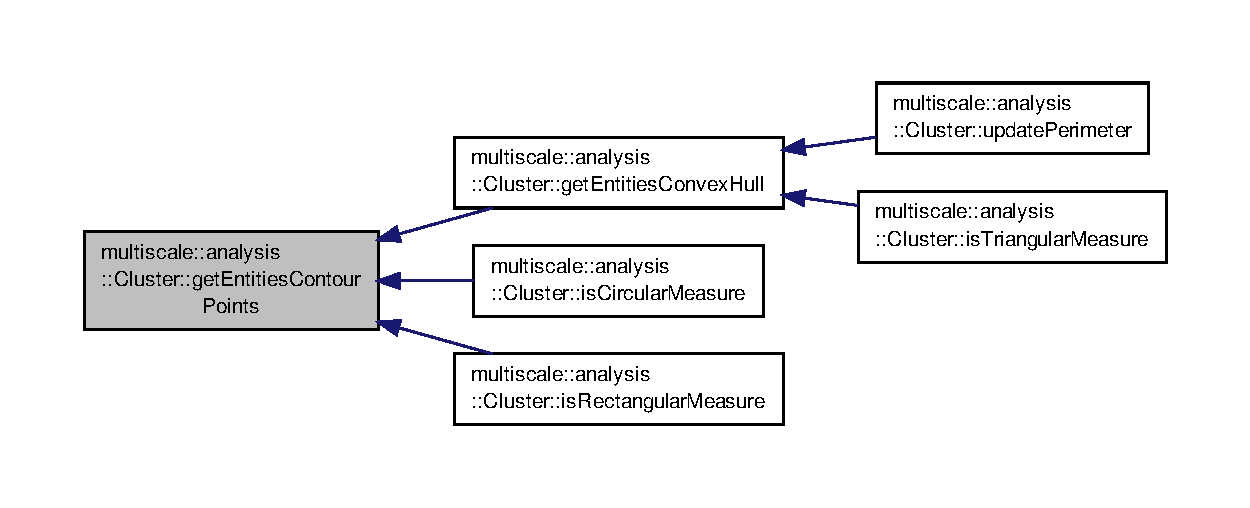
\includegraphics[width=350pt]{classmultiscale_1_1analysis_1_1Cluster_adbb1a108b2ae638fbba0450c7f7fee20_icgraph}
\end{center}
\end{figure}


\hypertarget{classmultiscale_1_1analysis_1_1Cluster_a9f43161c58d9e4a97f3a33807397b255}{\index{multiscale\-::analysis\-::\-Cluster@{multiscale\-::analysis\-::\-Cluster}!get\-Entities\-Convex\-Hull@{get\-Entities\-Convex\-Hull}}
\index{get\-Entities\-Convex\-Hull@{get\-Entities\-Convex\-Hull}!multiscale::analysis::Cluster@{multiscale\-::analysis\-::\-Cluster}}
\subsubsection[{get\-Entities\-Convex\-Hull}]{\setlength{\rightskip}{0pt plus 5cm}vector$<$ Point2f $>$ Cluster\-::get\-Entities\-Convex\-Hull (
\begin{DoxyParamCaption}
{}
\end{DoxyParamCaption}
)}}\label{classmultiscale_1_1analysis_1_1Cluster_a9f43161c58d9e4a97f3a33807397b255}


Get the convex hull enclosing the collection of entities' contour points. 



Definition at line 51 of file Cluster.\-cpp.



References multiscale\-::analysis\-::\-Spatial\-Entity\-Pseudo3\-D\-::\-C\-O\-N\-V\-E\-X\-\_\-\-H\-U\-L\-L\-\_\-\-C\-L\-O\-C\-K\-W\-I\-S\-E, entities, and get\-Entities\-Contour\-Points().



Referenced by multiscale\-::analysis\-::\-Cluster\-Detector\-::get\-Cluster\-Convex\-Hull(), is\-Triangular\-Measure(), update\-Centre\-Point(), and update\-Perimeter().



Here is the caller graph for this function\-:\nopagebreak
\begin{figure}[H]
\begin{center}
\leavevmode
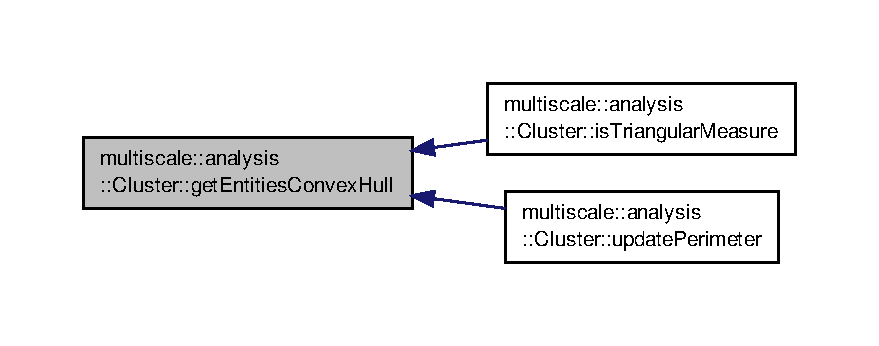
\includegraphics[width=350pt]{classmultiscale_1_1analysis_1_1Cluster_a9f43161c58d9e4a97f3a33807397b255_icgraph}
\end{center}
\end{figure}


\hypertarget{classmultiscale_1_1analysis_1_1Cluster_a4d93f85faf929336818248e1fd604fb6}{\index{multiscale\-::analysis\-::\-Cluster@{multiscale\-::analysis\-::\-Cluster}!get\-Min\-Area\-Enclosing\-Circle\-Centre@{get\-Min\-Area\-Enclosing\-Circle\-Centre}}
\index{get\-Min\-Area\-Enclosing\-Circle\-Centre@{get\-Min\-Area\-Enclosing\-Circle\-Centre}!multiscale::analysis::Cluster@{multiscale\-::analysis\-::\-Cluster}}
\subsubsection[{get\-Min\-Area\-Enclosing\-Circle\-Centre}]{\setlength{\rightskip}{0pt plus 5cm}Point2f Cluster\-::get\-Min\-Area\-Enclosing\-Circle\-Centre (
\begin{DoxyParamCaption}
{}
\end{DoxyParamCaption}
)}}\label{classmultiscale_1_1analysis_1_1Cluster_a4d93f85faf929336818248e1fd604fb6}


Get the minimum area enclosing circle centre. 



Definition at line 35 of file Cluster.\-cpp.



References min\-Area\-Enclosing\-Circle\-Centre, and multiscale\-::analysis\-::\-Spatial\-Entity\-Pseudo3\-D\-::update\-Measures\-If\-Required().



Referenced by multiscale\-::analysis\-::\-Simulation\-Cluster\-Detector\-::output\-Cluster\-Circular\-Shape().



Here is the caller graph for this function\-:\nopagebreak
\begin{figure}[H]
\begin{center}
\leavevmode
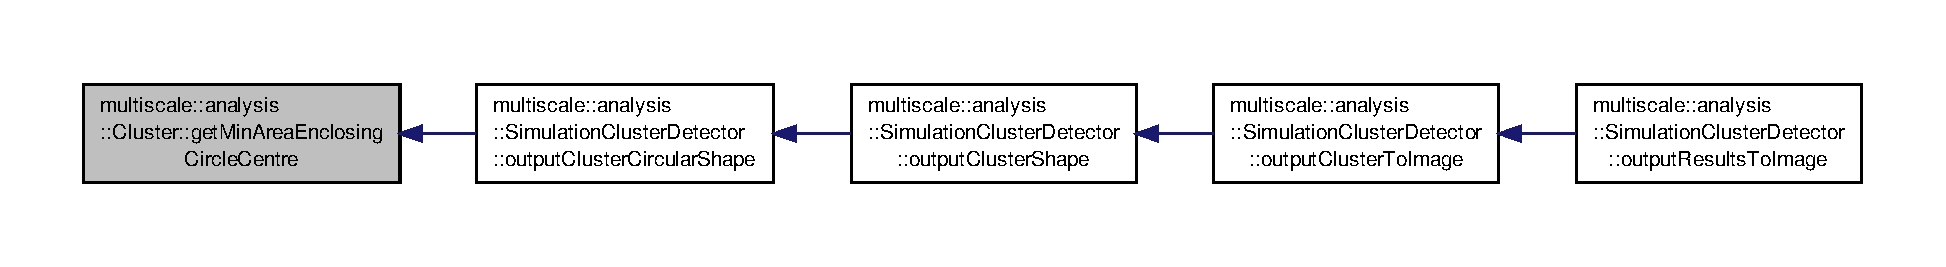
\includegraphics[width=350pt]{classmultiscale_1_1analysis_1_1Cluster_a4d93f85faf929336818248e1fd604fb6_icgraph}
\end{center}
\end{figure}


\hypertarget{classmultiscale_1_1analysis_1_1Cluster_aecf5fa56fa21e3b22130242694be744f}{\index{multiscale\-::analysis\-::\-Cluster@{multiscale\-::analysis\-::\-Cluster}!get\-Min\-Area\-Enclosing\-Circle\-Radius@{get\-Min\-Area\-Enclosing\-Circle\-Radius}}
\index{get\-Min\-Area\-Enclosing\-Circle\-Radius@{get\-Min\-Area\-Enclosing\-Circle\-Radius}!multiscale::analysis::Cluster@{multiscale\-::analysis\-::\-Cluster}}
\subsubsection[{get\-Min\-Area\-Enclosing\-Circle\-Radius}]{\setlength{\rightskip}{0pt plus 5cm}float Cluster\-::get\-Min\-Area\-Enclosing\-Circle\-Radius (
\begin{DoxyParamCaption}
{}
\end{DoxyParamCaption}
)}}\label{classmultiscale_1_1analysis_1_1Cluster_aecf5fa56fa21e3b22130242694be744f}


Get the minimum area enclosing circle radius. 



Definition at line 41 of file Cluster.\-cpp.



References min\-Area\-Enclosing\-Circle\-Radius, and multiscale\-::analysis\-::\-Spatial\-Entity\-Pseudo3\-D\-::update\-Measures\-If\-Required().



Referenced by multiscale\-::analysis\-::\-Simulation\-Cluster\-Detector\-::output\-Cluster\-Circular\-Shape().



Here is the caller graph for this function\-:\nopagebreak
\begin{figure}[H]
\begin{center}
\leavevmode
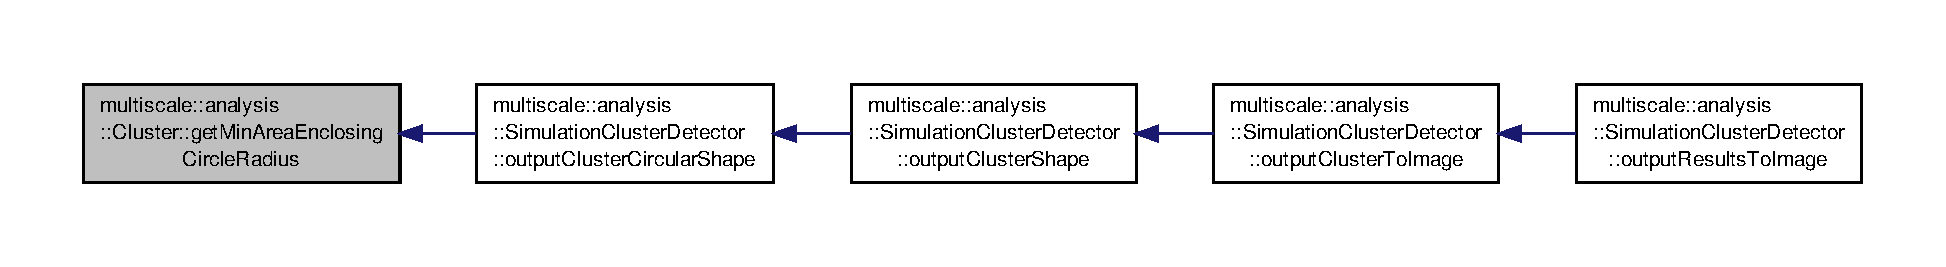
\includegraphics[width=350pt]{classmultiscale_1_1analysis_1_1Cluster_aecf5fa56fa21e3b22130242694be744f_icgraph}
\end{center}
\end{figure}


\hypertarget{classmultiscale_1_1analysis_1_1Cluster_a6417e3328622a848a7dedeebb5821750}{\index{multiscale\-::analysis\-::\-Cluster@{multiscale\-::analysis\-::\-Cluster}!get\-Min\-Area\-Enclosing\-Rect@{get\-Min\-Area\-Enclosing\-Rect}}
\index{get\-Min\-Area\-Enclosing\-Rect@{get\-Min\-Area\-Enclosing\-Rect}!multiscale::analysis::Cluster@{multiscale\-::analysis\-::\-Cluster}}
\subsubsection[{get\-Min\-Area\-Enclosing\-Rect}]{\setlength{\rightskip}{0pt plus 5cm}Rotated\-Rect Cluster\-::get\-Min\-Area\-Enclosing\-Rect (
\begin{DoxyParamCaption}
{}
\end{DoxyParamCaption}
)}}\label{classmultiscale_1_1analysis_1_1Cluster_a6417e3328622a848a7dedeebb5821750}


Get the minimum area enclosing rectangle. 



Definition at line 29 of file Cluster.\-cpp.



References min\-Area\-Enclosing\-Rect, and multiscale\-::analysis\-::\-Spatial\-Entity\-Pseudo3\-D\-::update\-Measures\-If\-Required().



Referenced by multiscale\-::analysis\-::\-Simulation\-Cluster\-Detector\-::output\-Cluster\-Rectangular\-Shape().



Here is the caller graph for this function\-:\nopagebreak
\begin{figure}[H]
\begin{center}
\leavevmode
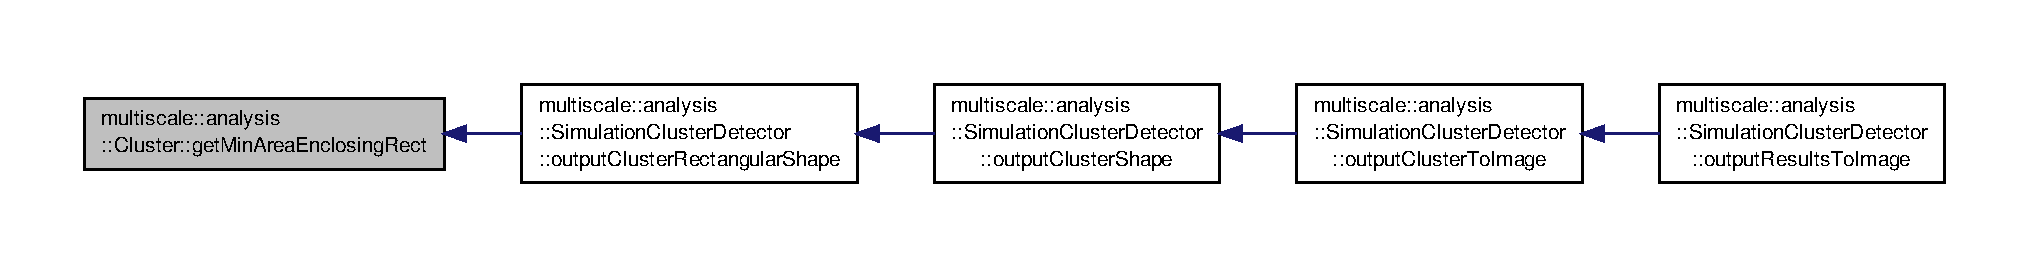
\includegraphics[width=350pt]{classmultiscale_1_1analysis_1_1Cluster_a6417e3328622a848a7dedeebb5821750_icgraph}
\end{center}
\end{figure}


\hypertarget{classmultiscale_1_1analysis_1_1Cluster_ab28150a739c35d66874c219fd38b462b}{\index{multiscale\-::analysis\-::\-Cluster@{multiscale\-::analysis\-::\-Cluster}!get\-Min\-Area\-Enclosing\-Triangle@{get\-Min\-Area\-Enclosing\-Triangle}}
\index{get\-Min\-Area\-Enclosing\-Triangle@{get\-Min\-Area\-Enclosing\-Triangle}!multiscale::analysis::Cluster@{multiscale\-::analysis\-::\-Cluster}}
\subsubsection[{get\-Min\-Area\-Enclosing\-Triangle}]{\setlength{\rightskip}{0pt plus 5cm}vector$<$ Point2f $>$ Cluster\-::get\-Min\-Area\-Enclosing\-Triangle (
\begin{DoxyParamCaption}
{}
\end{DoxyParamCaption}
)}}\label{classmultiscale_1_1analysis_1_1Cluster_ab28150a739c35d66874c219fd38b462b}


Get the minimum area enclosing triangle. 



Definition at line 23 of file Cluster.\-cpp.



References min\-Area\-Enclosing\-Triangle, and multiscale\-::analysis\-::\-Spatial\-Entity\-Pseudo3\-D\-::update\-Measures\-If\-Required().



Referenced by multiscale\-::analysis\-::\-Simulation\-Cluster\-Detector\-::output\-Cluster\-Triangular\-Shape().



Here is the caller graph for this function\-:\nopagebreak
\begin{figure}[H]
\begin{center}
\leavevmode
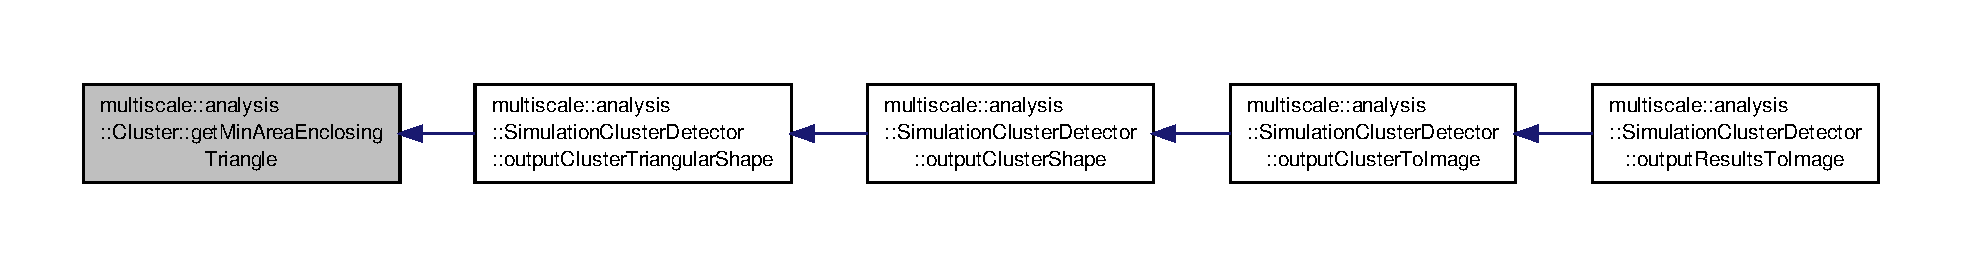
\includegraphics[width=350pt]{classmultiscale_1_1analysis_1_1Cluster_ab28150a739c35d66874c219fd38b462b_icgraph}
\end{center}
\end{figure}


\hypertarget{classmultiscale_1_1analysis_1_1Cluster_a3af6980def4fbfea38ccd86620f127f8}{\index{multiscale\-::analysis\-::\-Cluster@{multiscale\-::analysis\-::\-Cluster}!initialise@{initialise}}
\index{initialise@{initialise}!multiscale::analysis::Cluster@{multiscale\-::analysis\-::\-Cluster}}
\subsubsection[{initialise}]{\setlength{\rightskip}{0pt plus 5cm}void Cluster\-::initialise (
\begin{DoxyParamCaption}
{}
\end{DoxyParamCaption}
)\hspace{0.3cm}{\ttfamily [private]}}}\label{classmultiscale_1_1analysis_1_1Cluster_a3af6980def4fbfea38ccd86620f127f8}


Initialisation function for the class. 



Definition at line 69 of file Cluster.\-cpp.



References multiscale\-::analysis\-::\-Spatial\-Entity\-Pseudo3\-D\-::angle, multiscale\-::analysis\-::\-Spatial\-Entity\-Pseudo3\-D\-::clusteredness\-Degree, multiscale\-::analysis\-::\-Spatial\-Entity\-Pseudo3\-D\-::density, multiscale\-::analysis\-::\-Spatial\-Entity\-Pseudo3\-D\-::distance\-From\-Origin, entities, min\-Area\-Enclosing\-Circle\-Radius, min\-Area\-Enclosing\-Triangle, and multiscale\-::analysis\-::\-Spatial\-Entity\-Pseudo3\-D\-::update\-Flag.



Referenced by Cluster().



Here is the caller graph for this function\-:\nopagebreak
\begin{figure}[H]
\begin{center}
\leavevmode
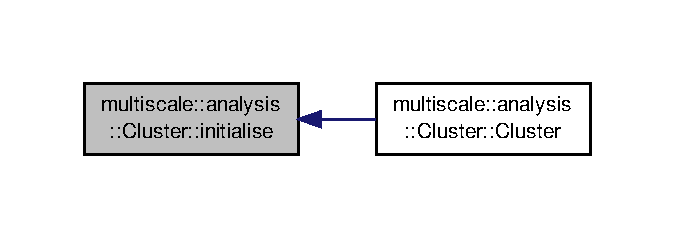
\includegraphics[width=324pt]{classmultiscale_1_1analysis_1_1Cluster_a3af6980def4fbfea38ccd86620f127f8_icgraph}
\end{center}
\end{figure}


\hypertarget{classmultiscale_1_1analysis_1_1Cluster_a579730478055ae93d659f268375a492d}{\index{multiscale\-::analysis\-::\-Cluster@{multiscale\-::analysis\-::\-Cluster}!is\-Circular\-Measure@{is\-Circular\-Measure}}
\index{is\-Circular\-Measure@{is\-Circular\-Measure}!multiscale::analysis::Cluster@{multiscale\-::analysis\-::\-Cluster}}
\subsubsection[{is\-Circular\-Measure}]{\setlength{\rightskip}{0pt plus 5cm}double Cluster\-::is\-Circular\-Measure (
\begin{DoxyParamCaption}
{}
\end{DoxyParamCaption}
)\hspace{0.3cm}{\ttfamily [override]}, {\ttfamily [private]}, {\ttfamily [virtual]}}}\label{classmultiscale_1_1analysis_1_1Cluster_a579730478055ae93d659f268375a492d}


Get the measure that the cluster has a circular shape. 



Implements \hyperlink{classmultiscale_1_1analysis_1_1SpatialEntityPseudo3D_a31066d1038679f8e9080719380403cad}{multiscale\-::analysis\-::\-Spatial\-Entity\-Pseudo3\-D}.



Definition at line 178 of file Cluster.\-cpp.



References get\-Entities\-Contour\-Points(), min\-Area\-Enclosing\-Circle\-Centre, min\-Area\-Enclosing\-Circle\-Radius, multiscale\-::analysis\-::\-Spatial\-Entity\-Pseudo3\-D\-::normalised\-Shape\-Measure(), and multiscale\-::\-Geometry2\-D\-::\-P\-I.

\hypertarget{classmultiscale_1_1analysis_1_1Cluster_aca93cb46704a3e824151e99b7a53d20d}{\index{multiscale\-::analysis\-::\-Cluster@{multiscale\-::analysis\-::\-Cluster}!is\-Rectangular\-Measure@{is\-Rectangular\-Measure}}
\index{is\-Rectangular\-Measure@{is\-Rectangular\-Measure}!multiscale::analysis::Cluster@{multiscale\-::analysis\-::\-Cluster}}
\subsubsection[{is\-Rectangular\-Measure}]{\setlength{\rightskip}{0pt plus 5cm}double Cluster\-::is\-Rectangular\-Measure (
\begin{DoxyParamCaption}
{}
\end{DoxyParamCaption}
)\hspace{0.3cm}{\ttfamily [override]}, {\ttfamily [private]}, {\ttfamily [virtual]}}}\label{classmultiscale_1_1analysis_1_1Cluster_aca93cb46704a3e824151e99b7a53d20d}


Get the measure that the cluster has a rectangular shape. 



Implements \hyperlink{classmultiscale_1_1analysis_1_1SpatialEntityPseudo3D_ad2984ec212e74437f3c7f3fc18ad555c}{multiscale\-::analysis\-::\-Spatial\-Entity\-Pseudo3\-D}.



Definition at line 167 of file Cluster.\-cpp.



References get\-Entities\-Contour\-Points(), min\-Area\-Enclosing\-Rect, and multiscale\-::analysis\-::\-Spatial\-Entity\-Pseudo3\-D\-::normalised\-Shape\-Measure().

\hypertarget{classmultiscale_1_1analysis_1_1Cluster_a28efcf050af76acb01619b36505b662e}{\index{multiscale\-::analysis\-::\-Cluster@{multiscale\-::analysis\-::\-Cluster}!is\-Triangular\-Measure@{is\-Triangular\-Measure}}
\index{is\-Triangular\-Measure@{is\-Triangular\-Measure}!multiscale::analysis::Cluster@{multiscale\-::analysis\-::\-Cluster}}
\subsubsection[{is\-Triangular\-Measure}]{\setlength{\rightskip}{0pt plus 5cm}double Cluster\-::is\-Triangular\-Measure (
\begin{DoxyParamCaption}
{}
\end{DoxyParamCaption}
)\hspace{0.3cm}{\ttfamily [override]}, {\ttfamily [private]}, {\ttfamily [virtual]}}}\label{classmultiscale_1_1analysis_1_1Cluster_a28efcf050af76acb01619b36505b662e}


Get the measure that the cluster has a triangular shape. 



Implements \hyperlink{classmultiscale_1_1analysis_1_1SpatialEntityPseudo3D_ac0e5bce32290f2595293bd7386e04de1}{multiscale\-::analysis\-::\-Spatial\-Entity\-Pseudo3\-D}.



Definition at line 159 of file Cluster.\-cpp.



References multiscale\-::\-Min\-Enclosing\-Triangle\-Finder\-::find(), get\-Entities\-Convex\-Hull(), min\-Area\-Enclosing\-Triangle, and multiscale\-::analysis\-::\-Spatial\-Entity\-Pseudo3\-D\-::normalised\-Shape\-Measure().

\hypertarget{classmultiscale_1_1analysis_1_1Cluster_a84033ee8d583d9195abbf42d5d420915}{\index{multiscale\-::analysis\-::\-Cluster@{multiscale\-::analysis\-::\-Cluster}!set\-Origin\-Dependent\-Members@{set\-Origin\-Dependent\-Members}}
\index{set\-Origin\-Dependent\-Members@{set\-Origin\-Dependent\-Members}!multiscale::analysis::Cluster@{multiscale\-::analysis\-::\-Cluster}}
\subsubsection[{set\-Origin\-Dependent\-Members}]{\setlength{\rightskip}{0pt plus 5cm}void Cluster\-::set\-Origin\-Dependent\-Members (
\begin{DoxyParamCaption}
\item[{double}]{distance\-From\-Origin, }
\item[{double}]{angle\-Wrt\-Origin}
\end{DoxyParamCaption}
)}}\label{classmultiscale_1_1analysis_1_1Cluster_a84033ee8d583d9195abbf42d5d420915}


Set the values of the origin dependent members. 


\begin{DoxyParams}{Parameters}
{\em distance\-From\-Origin} & Distance from the origin \\
\hline
{\em angle\-Wrt\-Origin} & Angle with respect to the origin \\
\hline
\end{DoxyParams}


Definition at line 62 of file Cluster.\-cpp.



References multiscale\-::analysis\-::\-Spatial\-Entity\-Pseudo3\-D\-::angle, multiscale\-::analysis\-::\-Spatial\-Entity\-Pseudo3\-D\-::distance\-From\-Origin, and validate\-Origin\-Dependent\-Values().



Referenced by multiscale\-::analysis\-::\-Cluster\-Detector\-::update\-Cluster\-Origin\-Dependent\-Values().



Here is the caller graph for this function\-:\nopagebreak
\begin{figure}[H]
\begin{center}
\leavevmode
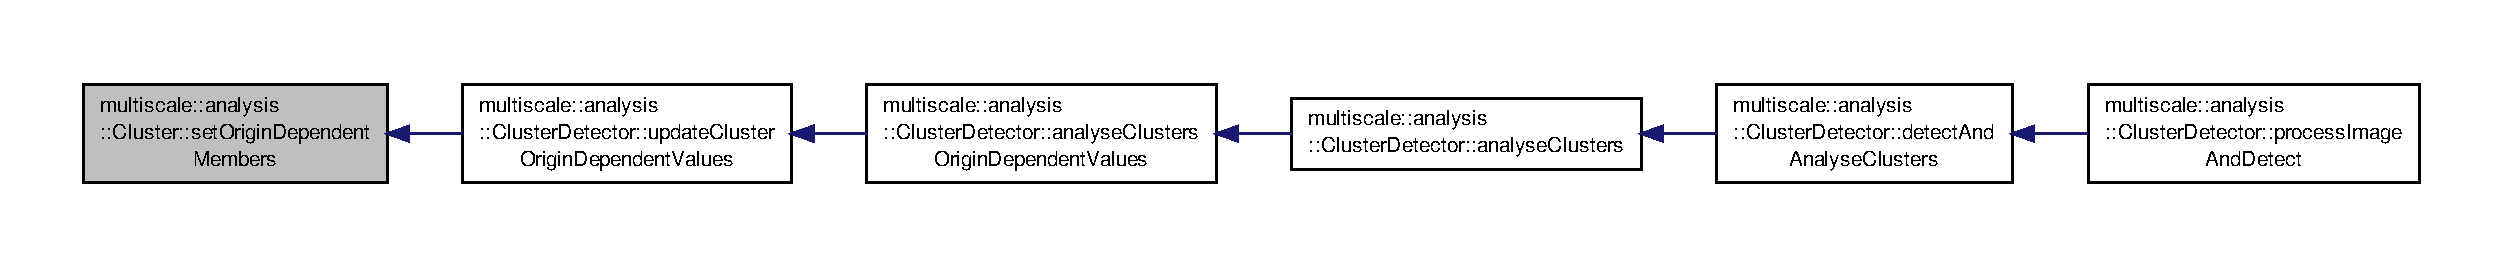
\includegraphics[width=350pt]{classmultiscale_1_1analysis_1_1Cluster_a84033ee8d583d9195abbf42d5d420915_icgraph}
\end{center}
\end{figure}


\hypertarget{classmultiscale_1_1analysis_1_1Cluster_a0a4531d371662e9c4149c10aa115fb49}{\index{multiscale\-::analysis\-::\-Cluster@{multiscale\-::analysis\-::\-Cluster}!type@{type}}
\index{type@{type}!multiscale::analysis::Cluster@{multiscale\-::analysis\-::\-Cluster}}
\subsubsection[{type}]{\setlength{\rightskip}{0pt plus 5cm}{\bf Spatial\-Entity\-Pseudo3\-D\-Type} Cluster\-::type (
\begin{DoxyParamCaption}
{}
\end{DoxyParamCaption}
)\hspace{0.3cm}{\ttfamily [override]}, {\ttfamily [private]}, {\ttfamily [virtual]}}}\label{classmultiscale_1_1analysis_1_1Cluster_a0a4531d371662e9c4149c10aa115fb49}


Return the type of the pseudo 3\-D spatial entity. 



Implements \hyperlink{classmultiscale_1_1analysis_1_1SpatialEntityPseudo3D_ac0d4656a44cc724c2cc7d34d8b15dbd8}{multiscale\-::analysis\-::\-Spatial\-Entity\-Pseudo3\-D}.



Definition at line 189 of file Cluster.\-cpp.

\hypertarget{classmultiscale_1_1analysis_1_1Cluster_a3128a3b20c28619ccdd6a25208b8c83e}{\index{multiscale\-::analysis\-::\-Cluster@{multiscale\-::analysis\-::\-Cluster}!update\-Area@{update\-Area}}
\index{update\-Area@{update\-Area}!multiscale::analysis::Cluster@{multiscale\-::analysis\-::\-Cluster}}
\subsubsection[{update\-Area}]{\setlength{\rightskip}{0pt plus 5cm}void Cluster\-::update\-Area (
\begin{DoxyParamCaption}
{}
\end{DoxyParamCaption}
)\hspace{0.3cm}{\ttfamily [override]}, {\ttfamily [private]}, {\ttfamily [virtual]}}}\label{classmultiscale_1_1analysis_1_1Cluster_a3128a3b20c28619ccdd6a25208b8c83e}


Update the value of the area. 



Implements \hyperlink{classmultiscale_1_1analysis_1_1SpatialEntityPseudo3D_aa8c1cd3248c8926edbb1b47006ded902}{multiscale\-::analysis\-::\-Spatial\-Entity\-Pseudo3\-D}.



Definition at line 136 of file Cluster.\-cpp.



References multiscale\-::analysis\-::\-Spatial\-Entity\-Pseudo3\-D\-::area, and entities.

\hypertarget{classmultiscale_1_1analysis_1_1Cluster_a1991d68cc9e76dab54c134df6beb59cb}{\index{multiscale\-::analysis\-::\-Cluster@{multiscale\-::analysis\-::\-Cluster}!update\-Centre\-Point@{update\-Centre\-Point}}
\index{update\-Centre\-Point@{update\-Centre\-Point}!multiscale::analysis::Cluster@{multiscale\-::analysis\-::\-Cluster}}
\subsubsection[{update\-Centre\-Point}]{\setlength{\rightskip}{0pt plus 5cm}void Cluster\-::update\-Centre\-Point (
\begin{DoxyParamCaption}
{}
\end{DoxyParamCaption}
)\hspace{0.3cm}{\ttfamily [override]}, {\ttfamily [private]}, {\ttfamily [virtual]}}}\label{classmultiscale_1_1analysis_1_1Cluster_a1991d68cc9e76dab54c134df6beb59cb}


Update the point defining the centre of the cluster. 



Implements \hyperlink{classmultiscale_1_1analysis_1_1SpatialEntityPseudo3D_a8e81fdb72e8510d8f77ce8b518a74843}{multiscale\-::analysis\-::\-Spatial\-Entity\-Pseudo3\-D}.



Definition at line 150 of file Cluster.\-cpp.



References multiscale\-::analysis\-::\-Spatial\-Entity\-Pseudo3\-D\-::centre, and get\-Entities\-Convex\-Hull().

\hypertarget{classmultiscale_1_1analysis_1_1Cluster_a2279d1567eec7c0b1e29cae26cfb4d73}{\index{multiscale\-::analysis\-::\-Cluster@{multiscale\-::analysis\-::\-Cluster}!update\-Clusteredness\-Degree@{update\-Clusteredness\-Degree}}
\index{update\-Clusteredness\-Degree@{update\-Clusteredness\-Degree}!multiscale::analysis::Cluster@{multiscale\-::analysis\-::\-Cluster}}
\subsubsection[{update\-Clusteredness\-Degree}]{\setlength{\rightskip}{0pt plus 5cm}void Cluster\-::update\-Clusteredness\-Degree (
\begin{DoxyParamCaption}
{}
\end{DoxyParamCaption}
)\hspace{0.3cm}{\ttfamily [override]}, {\ttfamily [private]}, {\ttfamily [virtual]}}}\label{classmultiscale_1_1analysis_1_1Cluster_a2279d1567eec7c0b1e29cae26cfb4d73}


Update the value of the clusteredness degree. 



Implements \hyperlink{classmultiscale_1_1analysis_1_1SpatialEntityPseudo3D_a750ba1b5e457d9d6504fc8320a76e002}{multiscale\-::analysis\-::\-Spatial\-Entity\-Pseudo3\-D}.



Definition at line 106 of file Cluster.\-cpp.



References multiscale\-::analysis\-::\-Spatial\-Entity\-Pseudo3\-D\-::clusteredness\-Degree, and entities.

\hypertarget{classmultiscale_1_1analysis_1_1Cluster_ac0300d9d05b0eb3aecd5724a14c2da41}{\index{multiscale\-::analysis\-::\-Cluster@{multiscale\-::analysis\-::\-Cluster}!update\-Density@{update\-Density}}
\index{update\-Density@{update\-Density}!multiscale::analysis::Cluster@{multiscale\-::analysis\-::\-Cluster}}
\subsubsection[{update\-Density}]{\setlength{\rightskip}{0pt plus 5cm}void Cluster\-::update\-Density (
\begin{DoxyParamCaption}
{}
\end{DoxyParamCaption}
)\hspace{0.3cm}{\ttfamily [override]}, {\ttfamily [private]}, {\ttfamily [virtual]}}}\label{classmultiscale_1_1analysis_1_1Cluster_ac0300d9d05b0eb3aecd5724a14c2da41}


Update the value of the pile up degree. 



Implements \hyperlink{classmultiscale_1_1analysis_1_1SpatialEntityPseudo3D_a28fa63c1101f3f5ba7a0001099ee3159}{multiscale\-::analysis\-::\-Spatial\-Entity\-Pseudo3\-D}.



Definition at line 126 of file Cluster.\-cpp.



References multiscale\-::analysis\-::\-Spatial\-Entity\-Pseudo3\-D\-::density, and entities.

\hypertarget{classmultiscale_1_1analysis_1_1Cluster_aadc520e4459f1ea6e22afd7c02d5f2ed}{\index{multiscale\-::analysis\-::\-Cluster@{multiscale\-::analysis\-::\-Cluster}!update\-Perimeter@{update\-Perimeter}}
\index{update\-Perimeter@{update\-Perimeter}!multiscale::analysis::Cluster@{multiscale\-::analysis\-::\-Cluster}}
\subsubsection[{update\-Perimeter}]{\setlength{\rightskip}{0pt plus 5cm}void Cluster\-::update\-Perimeter (
\begin{DoxyParamCaption}
{}
\end{DoxyParamCaption}
)\hspace{0.3cm}{\ttfamily [override]}, {\ttfamily [private]}, {\ttfamily [virtual]}}}\label{classmultiscale_1_1analysis_1_1Cluster_aadc520e4459f1ea6e22afd7c02d5f2ed}


Update the value of the perimeter. 



Implements \hyperlink{classmultiscale_1_1analysis_1_1SpatialEntityPseudo3D_acb00990b4b812367b7ae8f16028b8c32}{multiscale\-::analysis\-::\-Spatial\-Entity\-Pseudo3\-D}.



Definition at line 144 of file Cluster.\-cpp.



References get\-Entities\-Convex\-Hull(), and multiscale\-::analysis\-::\-Spatial\-Entity\-Pseudo3\-D\-::perimeter.

\hypertarget{classmultiscale_1_1analysis_1_1Cluster_a26b9c11e63bfdbfc837a35f68c5c40dd}{\index{multiscale\-::analysis\-::\-Cluster@{multiscale\-::analysis\-::\-Cluster}!validate\-Origin\-Dependent\-Values@{validate\-Origin\-Dependent\-Values}}
\index{validate\-Origin\-Dependent\-Values@{validate\-Origin\-Dependent\-Values}!multiscale::analysis::Cluster@{multiscale\-::analysis\-::\-Cluster}}
\subsubsection[{validate\-Origin\-Dependent\-Values}]{\setlength{\rightskip}{0pt plus 5cm}void Cluster\-::validate\-Origin\-Dependent\-Values (
\begin{DoxyParamCaption}
\item[{double}]{distance\-From\-Origin, }
\item[{double}]{angle\-Wrt\-Origin}
\end{DoxyParamCaption}
)\hspace{0.3cm}{\ttfamily [private]}}}\label{classmultiscale_1_1analysis_1_1Cluster_a26b9c11e63bfdbfc837a35f68c5c40dd}


Validate the origin dependent values (i.\-e. non-\/negative) 


\begin{DoxyParams}{Parameters}
{\em distance\-From\-Origin} & Distance from the origin \\
\hline
{\em angle\-Wrt\-Origin} & Angle with respect to the origin \\
\hline
\end{DoxyParams}


Definition at line 193 of file Cluster.\-cpp.



References are\-Valid\-Origin\-Dependent\-Values(), E\-R\-R\-\_\-\-O\-R\-I\-G\-I\-N\-\_\-\-D\-E\-P\-E\-N\-D\-E\-N\-T\-\_\-\-V\-A\-L\-U\-E\-S, and M\-S\-\_\-throw.



Referenced by set\-Origin\-Dependent\-Members().



Here is the caller graph for this function\-:\nopagebreak
\begin{figure}[H]
\begin{center}
\leavevmode
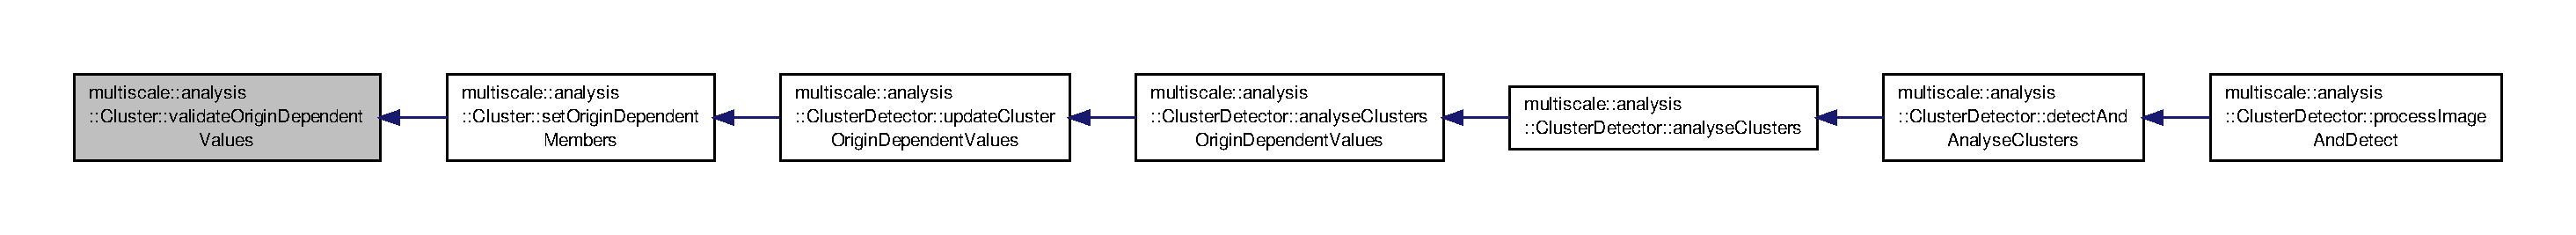
\includegraphics[width=350pt]{classmultiscale_1_1analysis_1_1Cluster_a26b9c11e63bfdbfc837a35f68c5c40dd_icgraph}
\end{center}
\end{figure}




\subsection{Member Data Documentation}
\hypertarget{classmultiscale_1_1analysis_1_1Cluster_a820298479651328fb79d92a65f7923d6}{\index{multiscale\-::analysis\-::\-Cluster@{multiscale\-::analysis\-::\-Cluster}!entities@{entities}}
\index{entities@{entities}!multiscale::analysis::Cluster@{multiscale\-::analysis\-::\-Cluster}}
\subsubsection[{entities}]{\setlength{\rightskip}{0pt plus 5cm}vector$<${\bf Entity}$>$ multiscale\-::analysis\-::\-Cluster\-::entities\hspace{0.3cm}{\ttfamily [private]}}}\label{classmultiscale_1_1analysis_1_1Cluster_a820298479651328fb79d92a65f7923d6}
Entities which belong to this cluster 

Definition at line 32 of file Cluster.\-hpp.



Referenced by add\-Entity(), get\-Entities(), get\-Entities\-Centre\-Points(), get\-Entities\-Contour\-Points(), get\-Entities\-Convex\-Hull(), initialise(), update\-Area(), update\-Clusteredness\-Degree(), and update\-Density().

\hypertarget{classmultiscale_1_1analysis_1_1Cluster_a0fa38fcc3f00730409400578829cddd8}{\index{multiscale\-::analysis\-::\-Cluster@{multiscale\-::analysis\-::\-Cluster}!E\-R\-R\-\_\-\-O\-R\-I\-G\-I\-N\-\_\-\-D\-E\-P\-E\-N\-D\-E\-N\-T\-\_\-\-V\-A\-L\-U\-E\-S@{E\-R\-R\-\_\-\-O\-R\-I\-G\-I\-N\-\_\-\-D\-E\-P\-E\-N\-D\-E\-N\-T\-\_\-\-V\-A\-L\-U\-E\-S}}
\index{E\-R\-R\-\_\-\-O\-R\-I\-G\-I\-N\-\_\-\-D\-E\-P\-E\-N\-D\-E\-N\-T\-\_\-\-V\-A\-L\-U\-E\-S@{E\-R\-R\-\_\-\-O\-R\-I\-G\-I\-N\-\_\-\-D\-E\-P\-E\-N\-D\-E\-N\-T\-\_\-\-V\-A\-L\-U\-E\-S}!multiscale::analysis::Cluster@{multiscale\-::analysis\-::\-Cluster}}
\subsubsection[{E\-R\-R\-\_\-\-O\-R\-I\-G\-I\-N\-\_\-\-D\-E\-P\-E\-N\-D\-E\-N\-T\-\_\-\-V\-A\-L\-U\-E\-S}]{\setlength{\rightskip}{0pt plus 5cm}const string Cluster\-::\-E\-R\-R\-\_\-\-O\-R\-I\-G\-I\-N\-\_\-\-D\-E\-P\-E\-N\-D\-E\-N\-T\-\_\-\-V\-A\-L\-U\-E\-S = \char`\"{}The origin dependent values are invalid (i.\-e. negative).\char`\"{}\hspace{0.3cm}{\ttfamily [static]}}}\label{classmultiscale_1_1analysis_1_1Cluster_a0fa38fcc3f00730409400578829cddd8}


Definition at line 123 of file Cluster.\-hpp.



Referenced by validate\-Origin\-Dependent\-Values().

\hypertarget{classmultiscale_1_1analysis_1_1Cluster_a546b8e93e3f1ef51a9932f8599639070}{\index{multiscale\-::analysis\-::\-Cluster@{multiscale\-::analysis\-::\-Cluster}!E\-R\-R\-\_\-\-U\-N\-D\-E\-F\-I\-N\-E\-D\-\_\-\-S\-H\-A\-P\-E@{E\-R\-R\-\_\-\-U\-N\-D\-E\-F\-I\-N\-E\-D\-\_\-\-S\-H\-A\-P\-E}}
\index{E\-R\-R\-\_\-\-U\-N\-D\-E\-F\-I\-N\-E\-D\-\_\-\-S\-H\-A\-P\-E@{E\-R\-R\-\_\-\-U\-N\-D\-E\-F\-I\-N\-E\-D\-\_\-\-S\-H\-A\-P\-E}!multiscale::analysis::Cluster@{multiscale\-::analysis\-::\-Cluster}}
\subsubsection[{E\-R\-R\-\_\-\-U\-N\-D\-E\-F\-I\-N\-E\-D\-\_\-\-S\-H\-A\-P\-E}]{\setlength{\rightskip}{0pt plus 5cm}const string Cluster\-::\-E\-R\-R\-\_\-\-U\-N\-D\-E\-F\-I\-N\-E\-D\-\_\-\-S\-H\-A\-P\-E = \char`\"{}The {\bf shape} of the given cluster is undefined.\char`\"{}\hspace{0.3cm}{\ttfamily [static]}}}\label{classmultiscale_1_1analysis_1_1Cluster_a546b8e93e3f1ef51a9932f8599639070}


Definition at line 122 of file Cluster.\-hpp.



Referenced by multiscale\-::analysis\-::\-Simulation\-Cluster\-Detector\-::output\-Cluster\-Shape().

\hypertarget{classmultiscale_1_1analysis_1_1Cluster_a47e672060b4025dcd07ebb9c5fd99f0c}{\index{multiscale\-::analysis\-::\-Cluster@{multiscale\-::analysis\-::\-Cluster}!min\-Area\-Enclosing\-Circle\-Centre@{min\-Area\-Enclosing\-Circle\-Centre}}
\index{min\-Area\-Enclosing\-Circle\-Centre@{min\-Area\-Enclosing\-Circle\-Centre}!multiscale::analysis::Cluster@{multiscale\-::analysis\-::\-Cluster}}
\subsubsection[{min\-Area\-Enclosing\-Circle\-Centre}]{\setlength{\rightskip}{0pt plus 5cm}Point2f multiscale\-::analysis\-::\-Cluster\-::min\-Area\-Enclosing\-Circle\-Centre\hspace{0.3cm}{\ttfamily [private]}}}\label{classmultiscale_1_1analysis_1_1Cluster_a47e672060b4025dcd07ebb9c5fd99f0c}
The minimum area enclosing circle centre point 

Definition at line 29 of file Cluster.\-hpp.



Referenced by get\-Min\-Area\-Enclosing\-Circle\-Centre(), and is\-Circular\-Measure().

\hypertarget{classmultiscale_1_1analysis_1_1Cluster_a070994481884a4c7f5aa4879ce7b0568}{\index{multiscale\-::analysis\-::\-Cluster@{multiscale\-::analysis\-::\-Cluster}!min\-Area\-Enclosing\-Circle\-Radius@{min\-Area\-Enclosing\-Circle\-Radius}}
\index{min\-Area\-Enclosing\-Circle\-Radius@{min\-Area\-Enclosing\-Circle\-Radius}!multiscale::analysis::Cluster@{multiscale\-::analysis\-::\-Cluster}}
\subsubsection[{min\-Area\-Enclosing\-Circle\-Radius}]{\setlength{\rightskip}{0pt plus 5cm}float multiscale\-::analysis\-::\-Cluster\-::min\-Area\-Enclosing\-Circle\-Radius\hspace{0.3cm}{\ttfamily [private]}}}\label{classmultiscale_1_1analysis_1_1Cluster_a070994481884a4c7f5aa4879ce7b0568}
The minimum area enclosing circle radius 

Definition at line 30 of file Cluster.\-hpp.



Referenced by get\-Min\-Area\-Enclosing\-Circle\-Radius(), initialise(), and is\-Circular\-Measure().

\hypertarget{classmultiscale_1_1analysis_1_1Cluster_aeb032303a79c6bd43385fcaad9c50742}{\index{multiscale\-::analysis\-::\-Cluster@{multiscale\-::analysis\-::\-Cluster}!min\-Area\-Enclosing\-Rect@{min\-Area\-Enclosing\-Rect}}
\index{min\-Area\-Enclosing\-Rect@{min\-Area\-Enclosing\-Rect}!multiscale::analysis::Cluster@{multiscale\-::analysis\-::\-Cluster}}
\subsubsection[{min\-Area\-Enclosing\-Rect}]{\setlength{\rightskip}{0pt plus 5cm}Rotated\-Rect multiscale\-::analysis\-::\-Cluster\-::min\-Area\-Enclosing\-Rect\hspace{0.3cm}{\ttfamily [private]}}}\label{classmultiscale_1_1analysis_1_1Cluster_aeb032303a79c6bd43385fcaad9c50742}
The minimum area enclosing rectangle 

Definition at line 27 of file Cluster.\-hpp.



Referenced by get\-Min\-Area\-Enclosing\-Rect(), and is\-Rectangular\-Measure().

\hypertarget{classmultiscale_1_1analysis_1_1Cluster_a7678d48581202c3ecc3f1283a1730dfa}{\index{multiscale\-::analysis\-::\-Cluster@{multiscale\-::analysis\-::\-Cluster}!min\-Area\-Enclosing\-Triangle@{min\-Area\-Enclosing\-Triangle}}
\index{min\-Area\-Enclosing\-Triangle@{min\-Area\-Enclosing\-Triangle}!multiscale::analysis::Cluster@{multiscale\-::analysis\-::\-Cluster}}
\subsubsection[{min\-Area\-Enclosing\-Triangle}]{\setlength{\rightskip}{0pt plus 5cm}vector$<$Point2f$>$ multiscale\-::analysis\-::\-Cluster\-::min\-Area\-Enclosing\-Triangle\hspace{0.3cm}{\ttfamily [private]}}}\label{classmultiscale_1_1analysis_1_1Cluster_a7678d48581202c3ecc3f1283a1730dfa}
The minimum area enclosing triangle 

Definition at line 25 of file Cluster.\-hpp.



Referenced by get\-Min\-Area\-Enclosing\-Triangle(), initialise(), and is\-Triangular\-Measure().



The documentation for this class was generated from the following files\-:\begin{DoxyCompactItemize}
\item 
/home/ovidiu/\-Repositories/git/multiscale/\-Multiscale/modules/analysis/spatial/include/multiscale/analysis/spatial/\hyperlink{analysis_2spatial_2include_2multiscale_2analysis_2spatial_2Cluster_8hpp}{Cluster.\-hpp}\item 
/home/ovidiu/\-Repositories/git/multiscale/\-Multiscale/modules/analysis/spatial/src/\hyperlink{Cluster_8cpp}{Cluster.\-cpp}\end{DoxyCompactItemize}

\hypertarget{classmultiscale_1_1analysis_1_1ClusterDetector}{\section{multiscale\-:\-:analysis\-:\-:Cluster\-Detector Class Reference}
\label{classmultiscale_1_1analysis_1_1ClusterDetector}\index{multiscale\-::analysis\-::\-Cluster\-Detector@{multiscale\-::analysis\-::\-Cluster\-Detector}}
}


Class for detecting clusters in 2\-D images.  




{\ttfamily \#include $<$Cluster\-Detector.\-hpp$>$}



Inheritance diagram for multiscale\-:\-:analysis\-:\-:Cluster\-Detector\-:\nopagebreak
\begin{figure}[H]
\begin{center}
\leavevmode
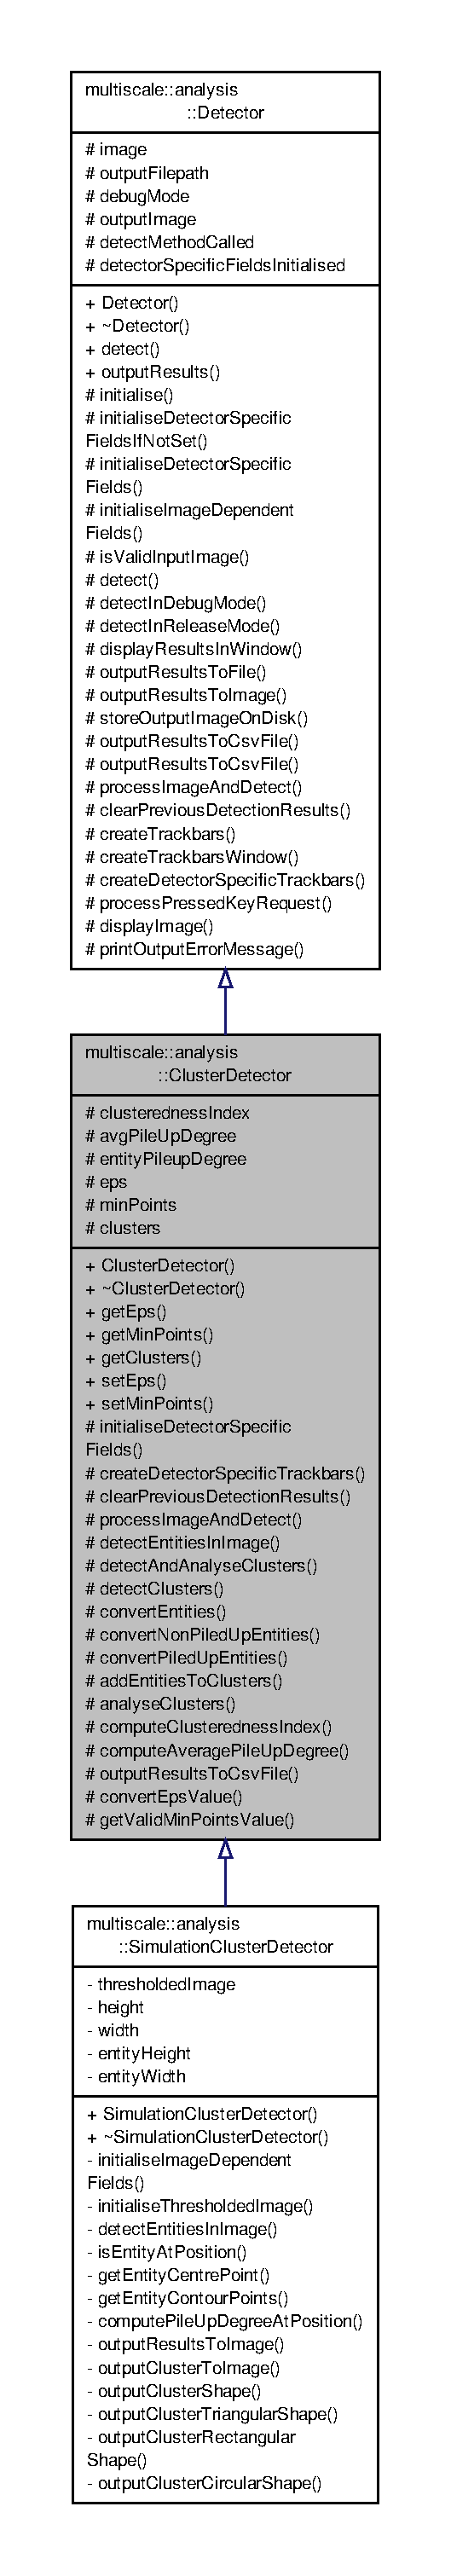
\includegraphics[height=550pt]{classmultiscale_1_1analysis_1_1ClusterDetector__inherit__graph}
\end{center}
\end{figure}


Collaboration diagram for multiscale\-:\-:analysis\-:\-:Cluster\-Detector\-:\nopagebreak
\begin{figure}[H]
\begin{center}
\leavevmode
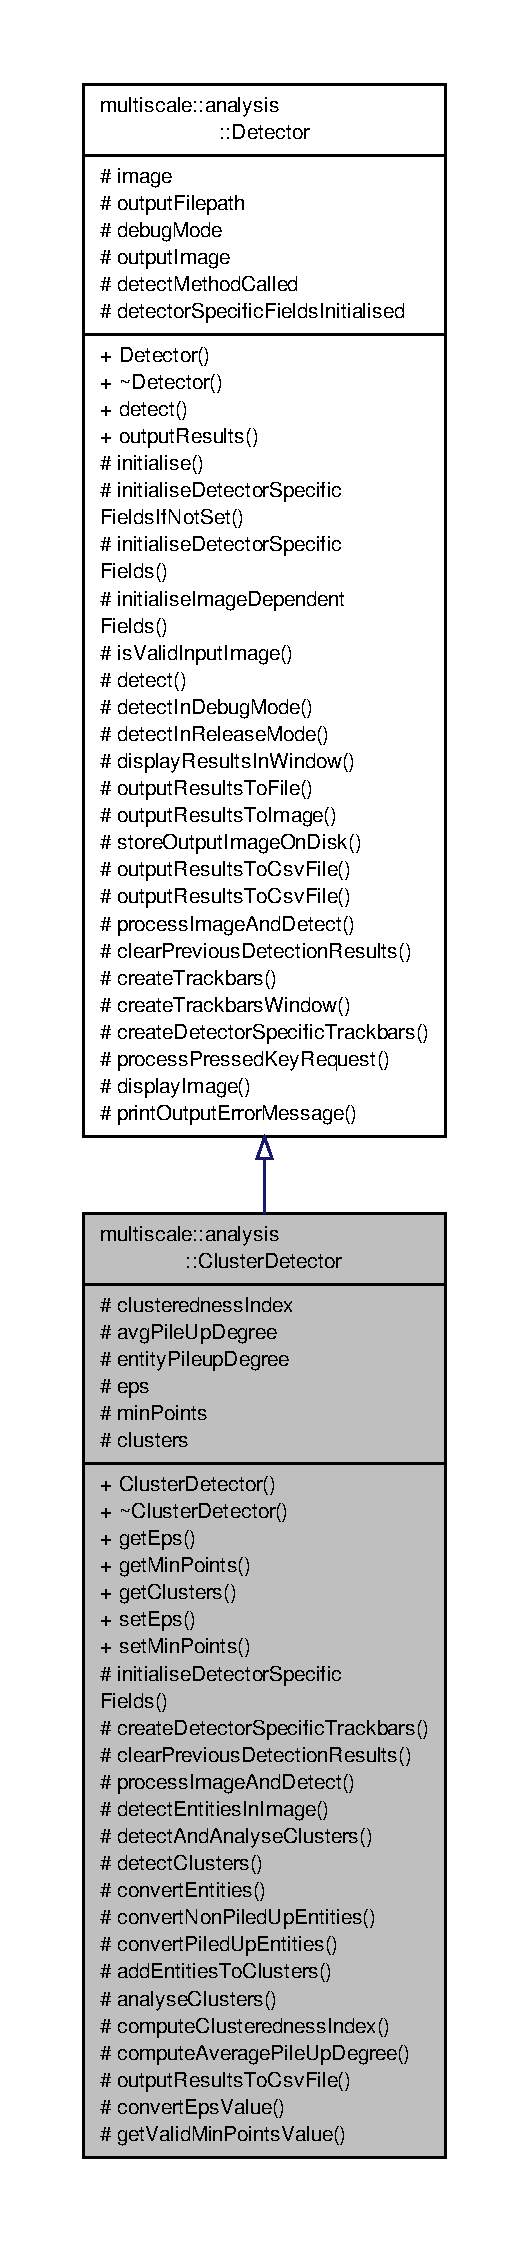
\includegraphics[height=550pt]{classmultiscale_1_1analysis_1_1ClusterDetector__coll__graph}
\end{center}
\end{figure}
\subsection*{Public Member Functions}
\begin{DoxyCompactItemize}
\item 
\hyperlink{classmultiscale_1_1analysis_1_1ClusterDetector_a2b5da40fb5e977f5bbfe046feeb1b124}{Cluster\-Detector} (int max\-Pileup\-Number, double max\-Pileup\-Intensity, bool \hyperlink{classmultiscale_1_1analysis_1_1Detector_a4b42f796957efd6ee0b8cf7645494a65}{debug\-Mode}=false)
\item 
virtual \hyperlink{classmultiscale_1_1analysis_1_1ClusterDetector_a18f5d5aab155a0a30137364749fb837c}{$\sim$\-Cluster\-Detector} ()
\item 
double \hyperlink{classmultiscale_1_1analysis_1_1ClusterDetector_a5f1699b100e7203720cb7fd1ef73cea1}{get\-Eps} ()
\begin{DoxyCompactList}\small\item\em Get the value of the clustering algorithm parameter eps. \end{DoxyCompactList}\item 
int \hyperlink{classmultiscale_1_1analysis_1_1ClusterDetector_af979c73c154bd42ef73d3328e80889ef}{get\-Min\-Points} ()
\begin{DoxyCompactList}\small\item\em Get the value of the clustering algorithm parameter Min\-Points. \end{DoxyCompactList}\item 
vector$<$ \hyperlink{classmultiscale_1_1analysis_1_1Cluster}{Cluster} $>$ const \& \hyperlink{classmultiscale_1_1analysis_1_1ClusterDetector_a0ed0e389d65161b7eef8f377efb20e5c}{get\-Clusters} ()
\begin{DoxyCompactList}\small\item\em Get a const reference to the vector of detected clusters. \end{DoxyCompactList}\item 
void \hyperlink{classmultiscale_1_1analysis_1_1ClusterDetector_a35eaa560c893a86c3149471f40c15979}{set\-Eps} (double \hyperlink{classmultiscale_1_1analysis_1_1ClusterDetector_a61e876f87d62245eada8f56d587d39cd}{eps})
\begin{DoxyCompactList}\small\item\em Set the value of the clustering algorithm parameter eps. \end{DoxyCompactList}\item 
void \hyperlink{classmultiscale_1_1analysis_1_1ClusterDetector_a190fd17d121e8c22c1ca6e4f5b7a213c}{set\-Min\-Points} (int \hyperlink{classmultiscale_1_1analysis_1_1ClusterDetector_aa94df1adc462be5931ec25ba24122fe9}{min\-Points})
\begin{DoxyCompactList}\small\item\em Set the value of the clustering algorithm parameter Min\-Points. \end{DoxyCompactList}\end{DoxyCompactItemize}
\subsection*{Protected Member Functions}
\begin{DoxyCompactItemize}
\item 
void \hyperlink{classmultiscale_1_1analysis_1_1ClusterDetector_a67751dd6e21750019a20648b6ba3c8f2}{initialise\-Detector\-Specific\-Fields} () override
\begin{DoxyCompactList}\small\item\em Initialise clustering values. \end{DoxyCompactList}\item 
void \hyperlink{classmultiscale_1_1analysis_1_1ClusterDetector_a7877cc5364f576e6a9cd96a6cd528cfc}{create\-Detector\-Specific\-Trackbars} () override
\begin{DoxyCompactList}\small\item\em Create the trackbars. \end{DoxyCompactList}\item 
void \hyperlink{classmultiscale_1_1analysis_1_1ClusterDetector_a5679e30f1ea35203963bf2baa8d7ed36}{clear\-Previous\-Detection\-Results} () override
\begin{DoxyCompactList}\small\item\em Clear the clusters from the previous detection. \end{DoxyCompactList}\item 
void \hyperlink{classmultiscale_1_1analysis_1_1ClusterDetector_a736847233c57cfa59abb953f70ef9209}{process\-Image\-And\-Detect} () override
\begin{DoxyCompactList}\small\item\em Process the provided image and detect clusters in it. \end{DoxyCompactList}\item 
virtual void \hyperlink{classmultiscale_1_1analysis_1_1ClusterDetector_a115f47c1f0855886ef5ca48acc111843}{detect\-Entities\-In\-Image} (vector$<$ \hyperlink{classmultiscale_1_1analysis_1_1Entity}{Entity} $>$ \&entities)=0
\begin{DoxyCompactList}\small\item\em Detect the entities in the image. \end{DoxyCompactList}\item 
void \hyperlink{classmultiscale_1_1analysis_1_1ClusterDetector_a46f98e066e74171774f0b6728118bc7b}{detect\-And\-Analyse\-Clusters} (const vector$<$ \hyperlink{classmultiscale_1_1analysis_1_1Entity}{Entity} $>$ \&entities, vector$<$ \hyperlink{classmultiscale_1_1analysis_1_1Cluster}{Cluster} $>$ \&\hyperlink{classmultiscale_1_1analysis_1_1ClusterDetector_aa81a8649bc743389c2fc1919d47eb5b3}{clusters})
\begin{DoxyCompactList}\small\item\em Detect and analyse the clusters of entities in the image. \end{DoxyCompactList}\item 
void \hyperlink{classmultiscale_1_1analysis_1_1ClusterDetector_a8c9c3ac0c3d8e924468a58f558984dda}{detect\-Clusters} (const vector$<$ \hyperlink{classmultiscale_1_1analysis_1_1Entity}{Entity} $>$ \&entities, vector$<$ int $>$ \&cluster\-Indexes, int \&nr\-Of\-Clusters)
\begin{DoxyCompactList}\small\item\em Detect the clusters of entities in the image. \end{DoxyCompactList}\item 
vector$<$ shared\-\_\-ptr$<$ \hyperlink{classmultiscale_1_1analysis_1_1DataPoint}{Data\-Point} $>$ $>$ \hyperlink{classmultiscale_1_1analysis_1_1ClusterDetector_aa45fe0a4a548b4d44407ee7f346e66d3}{convert\-Entities} (const vector$<$ \hyperlink{classmultiscale_1_1analysis_1_1Entity}{Entity} $>$ \&entities)
\begin{DoxyCompactList}\small\item\em Convert the entities to the format required by the \hyperlink{classmultiscale_1_1analysis_1_1DBSCAN}{D\-B\-S\-C\-A\-N} class. \end{DoxyCompactList}\item 
void \hyperlink{classmultiscale_1_1analysis_1_1ClusterDetector_a4b42b3de7411fe02c7871064497feef1}{convert\-Non\-Piled\-Up\-Entities} (const vector$<$ \hyperlink{classmultiscale_1_1analysis_1_1Entity}{Entity} $>$ \&entities, vector$<$ shared\-\_\-ptr$<$ \hyperlink{classmultiscale_1_1analysis_1_1DataPoint}{Data\-Point} $>$ $>$ \&data\-Points)
\begin{DoxyCompactList}\small\item\em Convert the non pile up entities to the format required by the \hyperlink{classmultiscale_1_1analysis_1_1DBSCAN}{D\-B\-S\-C\-A\-N} class. \end{DoxyCompactList}\item 
void \hyperlink{classmultiscale_1_1analysis_1_1ClusterDetector_a22ba21c341448af455111e718b058391}{convert\-Piled\-Up\-Entities} (const vector$<$ \hyperlink{classmultiscale_1_1analysis_1_1Entity}{Entity} $>$ \&entities, vector$<$ shared\-\_\-ptr$<$ \hyperlink{classmultiscale_1_1analysis_1_1DataPoint}{Data\-Point} $>$ $>$ \&data\-Points)
\begin{DoxyCompactList}\small\item\em Convert the entities to the required format by the \hyperlink{classmultiscale_1_1analysis_1_1DBSCAN}{D\-B\-S\-C\-A\-N} class. \end{DoxyCompactList}\item 
void \hyperlink{classmultiscale_1_1analysis_1_1ClusterDetector_aefc4d0736d8af4ab53f1e5e76440f447}{add\-Entities\-To\-Clusters} (const vector$<$ \hyperlink{classmultiscale_1_1analysis_1_1Entity}{Entity} $>$ \&entities, const vector$<$ int $>$ \&cluster\-Indexes, int nr\-Of\-Clusters, vector$<$ \hyperlink{classmultiscale_1_1analysis_1_1Cluster}{Cluster} $>$ \&\hyperlink{classmultiscale_1_1analysis_1_1ClusterDetector_aa81a8649bc743389c2fc1919d47eb5b3}{clusters})
\begin{DoxyCompactList}\small\item\em Add the entities to the clusters as indicated by the cluster\-Indexes parameter. \end{DoxyCompactList}\item 
void \hyperlink{classmultiscale_1_1analysis_1_1ClusterDetector_af994e960ba3cd76cc67e714ea276264a}{analyse\-Clusters} (vector$<$ \hyperlink{classmultiscale_1_1analysis_1_1Cluster}{Cluster} $>$ \&\hyperlink{classmultiscale_1_1analysis_1_1ClusterDetector_aa81a8649bc743389c2fc1919d47eb5b3}{clusters})
\begin{DoxyCompactList}\small\item\em Analyse the clusters. \end{DoxyCompactList}\item 
void \hyperlink{classmultiscale_1_1analysis_1_1ClusterDetector_affff27bd4559d1272913ff1bceb229b5}{analyse\-Clusters\-Origin\-Dependent\-Values} (vector$<$ \hyperlink{classmultiscale_1_1analysis_1_1Cluster}{Cluster} $>$ \&\hyperlink{classmultiscale_1_1analysis_1_1ClusterDetector_aa81a8649bc743389c2fc1919d47eb5b3}{clusters})
\begin{DoxyCompactList}\small\item\em Analyse the clusters and compute the origin dependent values. \end{DoxyCompactList}\item 
void \hyperlink{classmultiscale_1_1analysis_1_1ClusterDetector_ac7e008a7674205095f94b91c8d7cdccc}{update\-Cluster\-Origin\-Dependent\-Values} (\hyperlink{classmultiscale_1_1analysis_1_1Cluster}{Cluster} \&cluster, const vector$<$ Point $>$ \&cluster\-Convex\-Hull)
\begin{DoxyCompactList}\small\item\em Update the cluster and compute the origin dependent values considering the convex hull. \end{DoxyCompactList}\item 
vector$<$ Point $>$ \hyperlink{classmultiscale_1_1analysis_1_1ClusterDetector_a4a071efa7d7812c1db9ee577b7893902}{get\-Cluster\-Convex\-Hull} (\hyperlink{classmultiscale_1_1analysis_1_1Cluster}{Cluster} \&cluster)
\begin{DoxyCompactList}\small\item\em Return the convex hull of the given cluster. \end{DoxyCompactList}\item 
double \hyperlink{classmultiscale_1_1analysis_1_1ClusterDetector_aaa7937daf9872614e09b23cb4f6e5aa8}{compute\-Clusteredness\-Index} (const vector$<$ \hyperlink{classmultiscale_1_1analysis_1_1Cluster}{Cluster} $>$ \&\hyperlink{classmultiscale_1_1analysis_1_1ClusterDetector_aa81a8649bc743389c2fc1919d47eb5b3}{clusters})
\begin{DoxyCompactList}\small\item\em Compute the clusteredness index for all the entities detected in the image. \end{DoxyCompactList}\item 
double \hyperlink{classmultiscale_1_1analysis_1_1ClusterDetector_a1efab8446c79feb8a9285d895bb64b05}{compute\-Average\-Pile\-Up\-Degree} (vector$<$ \hyperlink{classmultiscale_1_1analysis_1_1Cluster}{Cluster} $>$ \&\hyperlink{classmultiscale_1_1analysis_1_1ClusterDetector_aa81a8649bc743389c2fc1919d47eb5b3}{clusters})
\begin{DoxyCompactList}\small\item\em Compute the average pile up degree for all entities in the image. \end{DoxyCompactList}\item 
void \hyperlink{classmultiscale_1_1analysis_1_1ClusterDetector_a6137f44f74afcac0584b1ff3f49f0ab8}{output\-Results\-To\-Csv\-File} (ofstream \&fout) override
\begin{DoxyCompactList}\small\item\em Output the information computed for the clusters to a csv file. \end{DoxyCompactList}\item 
double \hyperlink{classmultiscale_1_1analysis_1_1ClusterDetector_afccb86bfb93df00fff8408faea7a2651}{convert\-Eps\-Value} ()
\begin{DoxyCompactList}\small\item\em Convert the value of eps from integer to double. \end{DoxyCompactList}\item 
int \hyperlink{classmultiscale_1_1analysis_1_1ClusterDetector_ab1c2514fb8599f74bf010e81154a9bf7}{get\-Valid\-Min\-Points\-Value} ()
\begin{DoxyCompactList}\small\item\em Return non-\/zero value for min\-Points. \end{DoxyCompactList}\end{DoxyCompactItemize}
\subsection*{Protected Attributes}
\begin{DoxyCompactItemize}
\item 
double \hyperlink{classmultiscale_1_1analysis_1_1ClusterDetector_a5e2bf77041bd0d5047dd16c4632c16b7}{clusteredness\-Index}
\item 
double \hyperlink{classmultiscale_1_1analysis_1_1ClusterDetector_a6f6cfa50cf21ac400d41d6c6f2112bc9}{avg\-Pile\-Up\-Degree}
\item 
double \hyperlink{classmultiscale_1_1analysis_1_1ClusterDetector_aaa93a4b3a5a3c4279aa434669093ac40}{entity\-Pileup\-Degree}
\item 
int \hyperlink{classmultiscale_1_1analysis_1_1ClusterDetector_a61e876f87d62245eada8f56d587d39cd}{eps}
\item 
int \hyperlink{classmultiscale_1_1analysis_1_1ClusterDetector_aa94df1adc462be5931ec25ba24122fe9}{min\-Points}
\item 
vector$<$ \hyperlink{classmultiscale_1_1analysis_1_1Cluster}{Cluster} $>$ \hyperlink{classmultiscale_1_1analysis_1_1ClusterDetector_aa81a8649bc743389c2fc1919d47eb5b3}{clusters}
\end{DoxyCompactItemize}


\subsection{Detailed Description}
Class for detecting clusters in 2\-D images. 

Definition at line 34 of file Cluster\-Detector.\-hpp.



\subsection{Constructor \& Destructor Documentation}
\hypertarget{classmultiscale_1_1analysis_1_1ClusterDetector_a2b5da40fb5e977f5bbfe046feeb1b124}{\index{multiscale\-::analysis\-::\-Cluster\-Detector@{multiscale\-::analysis\-::\-Cluster\-Detector}!Cluster\-Detector@{Cluster\-Detector}}
\index{Cluster\-Detector@{Cluster\-Detector}!multiscale::analysis::ClusterDetector@{multiscale\-::analysis\-::\-Cluster\-Detector}}
\subsubsection[{Cluster\-Detector}]{\setlength{\rightskip}{0pt plus 5cm}Cluster\-Detector\-::\-Cluster\-Detector (
\begin{DoxyParamCaption}
\item[{int}]{max\-Pileup\-Number, }
\item[{double}]{max\-Pileup\-Intensity, }
\item[{bool}]{debug\-Mode = {\ttfamily false}}
\end{DoxyParamCaption}
)}}\label{classmultiscale_1_1analysis_1_1ClusterDetector_a2b5da40fb5e977f5bbfe046feeb1b124}

\begin{DoxyParams}{Parameters}
{\em debug\-Mode} & Flag indicating if detector should run in debug mode or not \\
\hline
{\em max\-Pileup\-Number} & The maximum number of entities which can occupy a grid position at the same time \\
\hline
{\em max\-Pileup\-Intensity} & The grayscale intensity of a maximally piled up grid position \\
\hline
\end{DoxyParams}


Definition at line 15 of file Cluster\-Detector.\-cpp.



References avg\-Pile\-Up\-Degree, clusteredness\-Index, entity\-Pileup\-Degree, eps, and min\-Points.

\hypertarget{classmultiscale_1_1analysis_1_1ClusterDetector_a18f5d5aab155a0a30137364749fb837c}{\index{multiscale\-::analysis\-::\-Cluster\-Detector@{multiscale\-::analysis\-::\-Cluster\-Detector}!$\sim$\-Cluster\-Detector@{$\sim$\-Cluster\-Detector}}
\index{$\sim$\-Cluster\-Detector@{$\sim$\-Cluster\-Detector}!multiscale::analysis::ClusterDetector@{multiscale\-::analysis\-::\-Cluster\-Detector}}
\subsubsection[{$\sim$\-Cluster\-Detector}]{\setlength{\rightskip}{0pt plus 5cm}Cluster\-Detector\-::$\sim$\-Cluster\-Detector (
\begin{DoxyParamCaption}
{}
\end{DoxyParamCaption}
)\hspace{0.3cm}{\ttfamily [virtual]}}}\label{classmultiscale_1_1analysis_1_1ClusterDetector_a18f5d5aab155a0a30137364749fb837c}


Definition at line 25 of file Cluster\-Detector.\-cpp.



\subsection{Member Function Documentation}
\hypertarget{classmultiscale_1_1analysis_1_1ClusterDetector_aefc4d0736d8af4ab53f1e5e76440f447}{\index{multiscale\-::analysis\-::\-Cluster\-Detector@{multiscale\-::analysis\-::\-Cluster\-Detector}!add\-Entities\-To\-Clusters@{add\-Entities\-To\-Clusters}}
\index{add\-Entities\-To\-Clusters@{add\-Entities\-To\-Clusters}!multiscale::analysis::ClusterDetector@{multiscale\-::analysis\-::\-Cluster\-Detector}}
\subsubsection[{add\-Entities\-To\-Clusters}]{\setlength{\rightskip}{0pt plus 5cm}void Cluster\-Detector\-::add\-Entities\-To\-Clusters (
\begin{DoxyParamCaption}
\item[{const vector$<$ {\bf Entity} $>$ \&}]{entities, }
\item[{const vector$<$ int $>$ \&}]{cluster\-Indexes, }
\item[{int}]{nr\-Of\-Clusters, }
\item[{vector$<$ {\bf Cluster} $>$ \&}]{clusters}
\end{DoxyParamCaption}
)\hspace{0.3cm}{\ttfamily [protected]}}}\label{classmultiscale_1_1analysis_1_1ClusterDetector_aefc4d0736d8af4ab53f1e5e76440f447}


Add the entities to the clusters as indicated by the cluster\-Indexes parameter. 

Add the entities to the clusters as indicated by the cluster\-Indexes parameter


\begin{DoxyParams}{Parameters}
{\em entities} & Entities detected in the image \\
\hline
{\em cluster\-Indexes} & Indexes to which cluster each entity belongs \\
\hline
{\em nr\-Of\-Clusters} & Total number of clusters \\
\hline
{\em clusters} & Collection of clusters, each one with the updated measures \\
\hline
\end{DoxyParams}


Definition at line 111 of file Cluster\-Detector.\-cpp.



Referenced by detect\-And\-Analyse\-Clusters().



Here is the caller graph for this function\-:\nopagebreak
\begin{figure}[H]
\begin{center}
\leavevmode
\includegraphics[width=350pt]{classmultiscale_1_1analysis_1_1ClusterDetector_aefc4d0736d8af4ab53f1e5e76440f447_icgraph}
\end{center}
\end{figure}


\hypertarget{classmultiscale_1_1analysis_1_1ClusterDetector_af994e960ba3cd76cc67e714ea276264a}{\index{multiscale\-::analysis\-::\-Cluster\-Detector@{multiscale\-::analysis\-::\-Cluster\-Detector}!analyse\-Clusters@{analyse\-Clusters}}
\index{analyse\-Clusters@{analyse\-Clusters}!multiscale::analysis::ClusterDetector@{multiscale\-::analysis\-::\-Cluster\-Detector}}
\subsubsection[{analyse\-Clusters}]{\setlength{\rightskip}{0pt plus 5cm}void Cluster\-Detector\-::analyse\-Clusters (
\begin{DoxyParamCaption}
\item[{vector$<$ {\bf Cluster} $>$ \&}]{clusters}
\end{DoxyParamCaption}
)\hspace{0.3cm}{\ttfamily [protected]}}}\label{classmultiscale_1_1analysis_1_1ClusterDetector_af994e960ba3cd76cc67e714ea276264a}


Analyse the clusters. 

Analyse the clusters and compute the angle and distance from the centre, average clusteredness degree and pile up degree


\begin{DoxyParams}{Parameters}
{\em clusters} & Collection of clusters, each one with the updated measures \\
\hline
\end{DoxyParams}


Definition at line 122 of file Cluster\-Detector.\-cpp.



References analyse\-Clusters\-Origin\-Dependent\-Values(), avg\-Pile\-Up\-Degree, clusteredness\-Index, compute\-Average\-Pile\-Up\-Degree(), and compute\-Clusteredness\-Index().



Referenced by detect\-And\-Analyse\-Clusters().



Here is the call graph for this function\-:\nopagebreak
\begin{figure}[H]
\begin{center}
\leavevmode
\includegraphics[width=350pt]{classmultiscale_1_1analysis_1_1ClusterDetector_af994e960ba3cd76cc67e714ea276264a_cgraph}
\end{center}
\end{figure}




Here is the caller graph for this function\-:\nopagebreak
\begin{figure}[H]
\begin{center}
\leavevmode
\includegraphics[width=350pt]{classmultiscale_1_1analysis_1_1ClusterDetector_af994e960ba3cd76cc67e714ea276264a_icgraph}
\end{center}
\end{figure}


\hypertarget{classmultiscale_1_1analysis_1_1ClusterDetector_affff27bd4559d1272913ff1bceb229b5}{\index{multiscale\-::analysis\-::\-Cluster\-Detector@{multiscale\-::analysis\-::\-Cluster\-Detector}!analyse\-Clusters\-Origin\-Dependent\-Values@{analyse\-Clusters\-Origin\-Dependent\-Values}}
\index{analyse\-Clusters\-Origin\-Dependent\-Values@{analyse\-Clusters\-Origin\-Dependent\-Values}!multiscale::analysis::ClusterDetector@{multiscale\-::analysis\-::\-Cluster\-Detector}}
\subsubsection[{analyse\-Clusters\-Origin\-Dependent\-Values}]{\setlength{\rightskip}{0pt plus 5cm}void Cluster\-Detector\-::analyse\-Clusters\-Origin\-Dependent\-Values (
\begin{DoxyParamCaption}
\item[{vector$<$ {\bf Cluster} $>$ \&}]{clusters}
\end{DoxyParamCaption}
)\hspace{0.3cm}{\ttfamily [protected]}}}\label{classmultiscale_1_1analysis_1_1ClusterDetector_affff27bd4559d1272913ff1bceb229b5}


Analyse the clusters and compute the origin dependent values. 

The values which depend on the origin point are the distance of the cluster from the centre and the angle


\begin{DoxyParams}{Parameters}
{\em clusters} & Collection of clusters, each one with the updated measures \\
\hline
\end{DoxyParams}


Definition at line 129 of file Cluster\-Detector.\-cpp.



References get\-Cluster\-Convex\-Hull(), and update\-Cluster\-Origin\-Dependent\-Values().



Referenced by analyse\-Clusters().



Here is the call graph for this function\-:\nopagebreak
\begin{figure}[H]
\begin{center}
\leavevmode
\includegraphics[width=350pt]{classmultiscale_1_1analysis_1_1ClusterDetector_affff27bd4559d1272913ff1bceb229b5_cgraph}
\end{center}
\end{figure}




Here is the caller graph for this function\-:\nopagebreak
\begin{figure}[H]
\begin{center}
\leavevmode
\includegraphics[width=350pt]{classmultiscale_1_1analysis_1_1ClusterDetector_affff27bd4559d1272913ff1bceb229b5_icgraph}
\end{center}
\end{figure}


\hypertarget{classmultiscale_1_1analysis_1_1ClusterDetector_a5679e30f1ea35203963bf2baa8d7ed36}{\index{multiscale\-::analysis\-::\-Cluster\-Detector@{multiscale\-::analysis\-::\-Cluster\-Detector}!clear\-Previous\-Detection\-Results@{clear\-Previous\-Detection\-Results}}
\index{clear\-Previous\-Detection\-Results@{clear\-Previous\-Detection\-Results}!multiscale::analysis::ClusterDetector@{multiscale\-::analysis\-::\-Cluster\-Detector}}
\subsubsection[{clear\-Previous\-Detection\-Results}]{\setlength{\rightskip}{0pt plus 5cm}void Cluster\-Detector\-::clear\-Previous\-Detection\-Results (
\begin{DoxyParamCaption}
{}
\end{DoxyParamCaption}
)\hspace{0.3cm}{\ttfamily [override]}, {\ttfamily [protected]}, {\ttfamily [virtual]}}}\label{classmultiscale_1_1analysis_1_1ClusterDetector_a5679e30f1ea35203963bf2baa8d7ed36}


Clear the clusters from the previous detection. 



Implements \hyperlink{classmultiscale_1_1analysis_1_1Detector_a3c2add35193ad09a0200003d0053da6b}{multiscale\-::analysis\-::\-Detector}.



Definition at line 61 of file Cluster\-Detector.\-cpp.



References clusters.

\hypertarget{classmultiscale_1_1analysis_1_1ClusterDetector_a1efab8446c79feb8a9285d895bb64b05}{\index{multiscale\-::analysis\-::\-Cluster\-Detector@{multiscale\-::analysis\-::\-Cluster\-Detector}!compute\-Average\-Pile\-Up\-Degree@{compute\-Average\-Pile\-Up\-Degree}}
\index{compute\-Average\-Pile\-Up\-Degree@{compute\-Average\-Pile\-Up\-Degree}!multiscale::analysis::ClusterDetector@{multiscale\-::analysis\-::\-Cluster\-Detector}}
\subsubsection[{compute\-Average\-Pile\-Up\-Degree}]{\setlength{\rightskip}{0pt plus 5cm}double Cluster\-Detector\-::compute\-Average\-Pile\-Up\-Degree (
\begin{DoxyParamCaption}
\item[{vector$<$ {\bf Cluster} $>$ \&}]{clusters}
\end{DoxyParamCaption}
)\hspace{0.3cm}{\ttfamily [protected]}}}\label{classmultiscale_1_1analysis_1_1ClusterDetector_a1efab8446c79feb8a9285d895bb64b05}


Compute the average pile up degree for all entities in the image. 

Compute the average pile up degree for all entities in the image as the sum of the average pile up degrees of all clusters divided by the number of clusters


\begin{DoxyParams}{Parameters}
{\em clusters} & Clusters of entities detected in the image \\
\hline
\end{DoxyParams}


Definition at line 162 of file Cluster\-Detector.\-cpp.



Referenced by analyse\-Clusters().



Here is the caller graph for this function\-:\nopagebreak
\begin{figure}[H]
\begin{center}
\leavevmode
\includegraphics[width=350pt]{classmultiscale_1_1analysis_1_1ClusterDetector_a1efab8446c79feb8a9285d895bb64b05_icgraph}
\end{center}
\end{figure}


\hypertarget{classmultiscale_1_1analysis_1_1ClusterDetector_aaa7937daf9872614e09b23cb4f6e5aa8}{\index{multiscale\-::analysis\-::\-Cluster\-Detector@{multiscale\-::analysis\-::\-Cluster\-Detector}!compute\-Clusteredness\-Index@{compute\-Clusteredness\-Index}}
\index{compute\-Clusteredness\-Index@{compute\-Clusteredness\-Index}!multiscale::analysis::ClusterDetector@{multiscale\-::analysis\-::\-Cluster\-Detector}}
\subsubsection[{compute\-Clusteredness\-Index}]{\setlength{\rightskip}{0pt plus 5cm}double Cluster\-Detector\-::compute\-Clusteredness\-Index (
\begin{DoxyParamCaption}
\item[{const vector$<$ {\bf Cluster} $>$ \&}]{clusters}
\end{DoxyParamCaption}
)\hspace{0.3cm}{\ttfamily [protected]}}}\label{classmultiscale_1_1analysis_1_1ClusterDetector_aaa7937daf9872614e09b23cb4f6e5aa8}


Compute the clusteredness index for all the entities detected in the image. 

Compute the clusteredness index for all the entities detected in the image using \hyperlink{classmultiscale_1_1analysis_1_1Silhouette}{Silhouette} cluster validity index


\begin{DoxyParams}{Parameters}
{\em clusters} & Collection of clusters, each one with the updated measures \\
\hline
\end{DoxyParams}


Definition at line 158 of file Cluster\-Detector.\-cpp.



References multiscale\-::analysis\-::\-Silhouette\-::compute\-Overall\-Average\-Measure().



Referenced by analyse\-Clusters().



Here is the call graph for this function\-:\nopagebreak
\begin{figure}[H]
\begin{center}
\leavevmode
\includegraphics[width=350pt]{classmultiscale_1_1analysis_1_1ClusterDetector_aaa7937daf9872614e09b23cb4f6e5aa8_cgraph}
\end{center}
\end{figure}




Here is the caller graph for this function\-:\nopagebreak
\begin{figure}[H]
\begin{center}
\leavevmode
\includegraphics[width=350pt]{classmultiscale_1_1analysis_1_1ClusterDetector_aaa7937daf9872614e09b23cb4f6e5aa8_icgraph}
\end{center}
\end{figure}


\hypertarget{classmultiscale_1_1analysis_1_1ClusterDetector_aa45fe0a4a548b4d44407ee7f346e66d3}{\index{multiscale\-::analysis\-::\-Cluster\-Detector@{multiscale\-::analysis\-::\-Cluster\-Detector}!convert\-Entities@{convert\-Entities}}
\index{convert\-Entities@{convert\-Entities}!multiscale::analysis::ClusterDetector@{multiscale\-::analysis\-::\-Cluster\-Detector}}
\subsubsection[{convert\-Entities}]{\setlength{\rightskip}{0pt plus 5cm}vector$<$ shared\-\_\-ptr$<$ {\bf Data\-Point} $>$ $>$ Cluster\-Detector\-::convert\-Entities (
\begin{DoxyParamCaption}
\item[{const vector$<$ {\bf Entity} $>$ \&}]{entities}
\end{DoxyParamCaption}
)\hspace{0.3cm}{\ttfamily [protected]}}}\label{classmultiscale_1_1analysis_1_1ClusterDetector_aa45fe0a4a548b4d44407ee7f346e66d3}


Convert the entities to the format required by the \hyperlink{classmultiscale_1_1analysis_1_1DBSCAN}{D\-B\-S\-C\-A\-N} class. 


\begin{DoxyParams}{Parameters}
{\em entities} & Entities detected in the image \\
\hline
\end{DoxyParams}


Definition at line 85 of file Cluster\-Detector.\-cpp.



References convert\-Non\-Piled\-Up\-Entities(), and convert\-Piled\-Up\-Entities().



Referenced by detect\-Clusters().



Here is the call graph for this function\-:\nopagebreak
\begin{figure}[H]
\begin{center}
\leavevmode
\includegraphics[width=350pt]{classmultiscale_1_1analysis_1_1ClusterDetector_aa45fe0a4a548b4d44407ee7f346e66d3_cgraph}
\end{center}
\end{figure}




Here is the caller graph for this function\-:\nopagebreak
\begin{figure}[H]
\begin{center}
\leavevmode
\includegraphics[width=350pt]{classmultiscale_1_1analysis_1_1ClusterDetector_aa45fe0a4a548b4d44407ee7f346e66d3_icgraph}
\end{center}
\end{figure}


\hypertarget{classmultiscale_1_1analysis_1_1ClusterDetector_afccb86bfb93df00fff8408faea7a2651}{\index{multiscale\-::analysis\-::\-Cluster\-Detector@{multiscale\-::analysis\-::\-Cluster\-Detector}!convert\-Eps\-Value@{convert\-Eps\-Value}}
\index{convert\-Eps\-Value@{convert\-Eps\-Value}!multiscale::analysis::ClusterDetector@{multiscale\-::analysis\-::\-Cluster\-Detector}}
\subsubsection[{convert\-Eps\-Value}]{\setlength{\rightskip}{0pt plus 5cm}double Cluster\-Detector\-::convert\-Eps\-Value (
\begin{DoxyParamCaption}
{}
\end{DoxyParamCaption}
)\hspace{0.3cm}{\ttfamily [protected]}}}\label{classmultiscale_1_1analysis_1_1ClusterDetector_afccb86bfb93df00fff8408faea7a2651}


Convert the value of eps from integer to double. 



Definition at line 191 of file Cluster\-Detector.\-cpp.



References eps, E\-P\-S\-\_\-\-M\-A\-X, E\-P\-S\-\_\-\-M\-I\-N, E\-P\-S\-\_\-\-R\-E\-A\-L\-\_\-\-M\-A\-X, and E\-P\-S\-\_\-\-R\-E\-A\-L\-\_\-\-M\-I\-N.



Referenced by detect\-Clusters(), and get\-Eps().



Here is the caller graph for this function\-:\nopagebreak
\begin{figure}[H]
\begin{center}
\leavevmode
\includegraphics[width=350pt]{classmultiscale_1_1analysis_1_1ClusterDetector_afccb86bfb93df00fff8408faea7a2651_icgraph}
\end{center}
\end{figure}


\hypertarget{classmultiscale_1_1analysis_1_1ClusterDetector_a4b42b3de7411fe02c7871064497feef1}{\index{multiscale\-::analysis\-::\-Cluster\-Detector@{multiscale\-::analysis\-::\-Cluster\-Detector}!convert\-Non\-Piled\-Up\-Entities@{convert\-Non\-Piled\-Up\-Entities}}
\index{convert\-Non\-Piled\-Up\-Entities@{convert\-Non\-Piled\-Up\-Entities}!multiscale::analysis::ClusterDetector@{multiscale\-::analysis\-::\-Cluster\-Detector}}
\subsubsection[{convert\-Non\-Piled\-Up\-Entities}]{\setlength{\rightskip}{0pt plus 5cm}void Cluster\-Detector\-::convert\-Non\-Piled\-Up\-Entities (
\begin{DoxyParamCaption}
\item[{const vector$<$ {\bf Entity} $>$ \&}]{entities, }
\item[{vector$<$ shared\-\_\-ptr$<$ {\bf Data\-Point} $>$ $>$ \&}]{data\-Points}
\end{DoxyParamCaption}
)\hspace{0.3cm}{\ttfamily [protected]}}}\label{classmultiscale_1_1analysis_1_1ClusterDetector_a4b42b3de7411fe02c7871064497feef1}


Convert the non pile up entities to the format required by the \hyperlink{classmultiscale_1_1analysis_1_1DBSCAN}{D\-B\-S\-C\-A\-N} class. 


\begin{DoxyParams}{Parameters}
{\em entities} & Entities detected in the image \\
\hline
{\em data\-Points} & Collection of \hyperlink{classmultiscale_1_1analysis_1_1DataPoint}{Data\-Point} instances required by the \hyperlink{classmultiscale_1_1analysis_1_1DBSCAN}{D\-B\-S\-C\-A\-N} class \\
\hline
\end{DoxyParams}


Definition at line 94 of file Cluster\-Detector.\-cpp.



Referenced by convert\-Entities().



Here is the caller graph for this function\-:\nopagebreak
\begin{figure}[H]
\begin{center}
\leavevmode
\includegraphics[width=350pt]{classmultiscale_1_1analysis_1_1ClusterDetector_a4b42b3de7411fe02c7871064497feef1_icgraph}
\end{center}
\end{figure}


\hypertarget{classmultiscale_1_1analysis_1_1ClusterDetector_a22ba21c341448af455111e718b058391}{\index{multiscale\-::analysis\-::\-Cluster\-Detector@{multiscale\-::analysis\-::\-Cluster\-Detector}!convert\-Piled\-Up\-Entities@{convert\-Piled\-Up\-Entities}}
\index{convert\-Piled\-Up\-Entities@{convert\-Piled\-Up\-Entities}!multiscale::analysis::ClusterDetector@{multiscale\-::analysis\-::\-Cluster\-Detector}}
\subsubsection[{convert\-Piled\-Up\-Entities}]{\setlength{\rightskip}{0pt plus 5cm}void Cluster\-Detector\-::convert\-Piled\-Up\-Entities (
\begin{DoxyParamCaption}
\item[{const vector$<$ {\bf Entity} $>$ \&}]{entities, }
\item[{vector$<$ shared\-\_\-ptr$<$ {\bf Data\-Point} $>$ $>$ \&}]{data\-Points}
\end{DoxyParamCaption}
)\hspace{0.3cm}{\ttfamily [protected]}}}\label{classmultiscale_1_1analysis_1_1ClusterDetector_a22ba21c341448af455111e718b058391}


Convert the entities to the required format by the \hyperlink{classmultiscale_1_1analysis_1_1DBSCAN}{D\-B\-S\-C\-A\-N} class. 


\begin{DoxyParams}{Parameters}
{\em entities} & Entities detected in the image \\
\hline
{\em data\-Points} & Collection of \hyperlink{classmultiscale_1_1analysis_1_1DataPoint}{Data\-Point} instances required by the \hyperlink{classmultiscale_1_1analysis_1_1DBSCAN}{D\-B\-S\-C\-A\-N} class \\
\hline
\end{DoxyParams}


Definition at line 100 of file Cluster\-Detector.\-cpp.



Referenced by convert\-Entities().



Here is the caller graph for this function\-:\nopagebreak
\begin{figure}[H]
\begin{center}
\leavevmode
\includegraphics[width=350pt]{classmultiscale_1_1analysis_1_1ClusterDetector_a22ba21c341448af455111e718b058391_icgraph}
\end{center}
\end{figure}


\hypertarget{classmultiscale_1_1analysis_1_1ClusterDetector_a7877cc5364f576e6a9cd96a6cd528cfc}{\index{multiscale\-::analysis\-::\-Cluster\-Detector@{multiscale\-::analysis\-::\-Cluster\-Detector}!create\-Detector\-Specific\-Trackbars@{create\-Detector\-Specific\-Trackbars}}
\index{create\-Detector\-Specific\-Trackbars@{create\-Detector\-Specific\-Trackbars}!multiscale::analysis::ClusterDetector@{multiscale\-::analysis\-::\-Cluster\-Detector}}
\subsubsection[{create\-Detector\-Specific\-Trackbars}]{\setlength{\rightskip}{0pt plus 5cm}void Cluster\-Detector\-::create\-Detector\-Specific\-Trackbars (
\begin{DoxyParamCaption}
{}
\end{DoxyParamCaption}
)\hspace{0.3cm}{\ttfamily [override]}, {\ttfamily [protected]}, {\ttfamily [virtual]}}}\label{classmultiscale_1_1analysis_1_1ClusterDetector_a7877cc5364f576e6a9cd96a6cd528cfc}


Create the trackbars. 



Implements \hyperlink{classmultiscale_1_1analysis_1_1Detector_a930ad07f5b8d9f21e6758341f71ae31a}{multiscale\-::analysis\-::\-Detector}.



Definition at line 56 of file Cluster\-Detector.\-cpp.



References eps, E\-P\-S\-\_\-\-M\-A\-X, M\-I\-N\-\_\-\-P\-O\-I\-N\-T\-S\-\_\-\-M\-A\-X, min\-Points, T\-R\-A\-C\-K\-B\-A\-R\-\_\-\-E\-P\-S, T\-R\-A\-C\-K\-B\-A\-R\-\_\-\-M\-I\-N\-P\-O\-I\-N\-T\-S, and W\-I\-N\-\_\-\-O\-U\-T\-P\-U\-T\-\_\-\-I\-M\-A\-G\-E.

\hypertarget{classmultiscale_1_1analysis_1_1ClusterDetector_a46f98e066e74171774f0b6728118bc7b}{\index{multiscale\-::analysis\-::\-Cluster\-Detector@{multiscale\-::analysis\-::\-Cluster\-Detector}!detect\-And\-Analyse\-Clusters@{detect\-And\-Analyse\-Clusters}}
\index{detect\-And\-Analyse\-Clusters@{detect\-And\-Analyse\-Clusters}!multiscale::analysis::ClusterDetector@{multiscale\-::analysis\-::\-Cluster\-Detector}}
\subsubsection[{detect\-And\-Analyse\-Clusters}]{\setlength{\rightskip}{0pt plus 5cm}void Cluster\-Detector\-::detect\-And\-Analyse\-Clusters (
\begin{DoxyParamCaption}
\item[{const vector$<$ {\bf Entity} $>$ \&}]{entities, }
\item[{vector$<$ {\bf Cluster} $>$ \&}]{clusters}
\end{DoxyParamCaption}
)\hspace{0.3cm}{\ttfamily [protected]}}}\label{classmultiscale_1_1analysis_1_1ClusterDetector_a46f98e066e74171774f0b6728118bc7b}


Detect and analyse the clusters of entities in the image. 

Detect and analyse the clusters of entities in the image


\begin{DoxyParams}{Parameters}
{\em entities} & Entities detected in the image \\
\hline
{\em clusters} & Clusters of entities detected in the image \\
\hline
\end{DoxyParams}


Definition at line 72 of file Cluster\-Detector.\-cpp.



References add\-Entities\-To\-Clusters(), analyse\-Clusters(), C\-L\-U\-S\-T\-E\-R\-I\-N\-G\-\_\-\-U\-N\-C\-L\-A\-S\-S\-I\-F\-I\-E\-D, and detect\-Clusters().



Referenced by process\-Image\-And\-Detect().



Here is the call graph for this function\-:\nopagebreak
\begin{figure}[H]
\begin{center}
\leavevmode
\includegraphics[width=350pt]{classmultiscale_1_1analysis_1_1ClusterDetector_a46f98e066e74171774f0b6728118bc7b_cgraph}
\end{center}
\end{figure}




Here is the caller graph for this function\-:\nopagebreak
\begin{figure}[H]
\begin{center}
\leavevmode
\includegraphics[width=350pt]{classmultiscale_1_1analysis_1_1ClusterDetector_a46f98e066e74171774f0b6728118bc7b_icgraph}
\end{center}
\end{figure}


\hypertarget{classmultiscale_1_1analysis_1_1ClusterDetector_a8c9c3ac0c3d8e924468a58f558984dda}{\index{multiscale\-::analysis\-::\-Cluster\-Detector@{multiscale\-::analysis\-::\-Cluster\-Detector}!detect\-Clusters@{detect\-Clusters}}
\index{detect\-Clusters@{detect\-Clusters}!multiscale::analysis::ClusterDetector@{multiscale\-::analysis\-::\-Cluster\-Detector}}
\subsubsection[{detect\-Clusters}]{\setlength{\rightskip}{0pt plus 5cm}void Cluster\-Detector\-::detect\-Clusters (
\begin{DoxyParamCaption}
\item[{const vector$<$ {\bf Entity} $>$ \&}]{entities, }
\item[{vector$<$ int $>$ \&}]{cluster\-Indexes, }
\item[{int \&}]{nr\-Of\-Clusters}
\end{DoxyParamCaption}
)\hspace{0.3cm}{\ttfamily [protected]}}}\label{classmultiscale_1_1analysis_1_1ClusterDetector_a8c9c3ac0c3d8e924468a58f558984dda}


Detect the clusters of entities in the image. 

Detect the clusters of entities in the image using Density Based scan (D\-Bscan) clustering algorithm Clusters start from index 1, because cluster 0 contains only noise data/points.


\begin{DoxyParams}{Parameters}
{\em entities} & Entities detected in the image \\
\hline
{\em cluster\-Indexes} & Indexes to which cluster each entity belongs \\
\hline
{\em nr\-Of\-Clusters} & Total number of clusters \\
\hline
\end{DoxyParams}


Definition at line 81 of file Cluster\-Detector.\-cpp.



References convert\-Entities(), convert\-Eps\-Value(), get\-Valid\-Min\-Points\-Value(), and multiscale\-::analysis\-::\-D\-B\-S\-C\-A\-N\-::run().



Referenced by detect\-And\-Analyse\-Clusters().



Here is the call graph for this function\-:\nopagebreak
\begin{figure}[H]
\begin{center}
\leavevmode
\includegraphics[width=350pt]{classmultiscale_1_1analysis_1_1ClusterDetector_a8c9c3ac0c3d8e924468a58f558984dda_cgraph}
\end{center}
\end{figure}




Here is the caller graph for this function\-:\nopagebreak
\begin{figure}[H]
\begin{center}
\leavevmode
\includegraphics[width=350pt]{classmultiscale_1_1analysis_1_1ClusterDetector_a8c9c3ac0c3d8e924468a58f558984dda_icgraph}
\end{center}
\end{figure}


\hypertarget{classmultiscale_1_1analysis_1_1ClusterDetector_a115f47c1f0855886ef5ca48acc111843}{\index{multiscale\-::analysis\-::\-Cluster\-Detector@{multiscale\-::analysis\-::\-Cluster\-Detector}!detect\-Entities\-In\-Image@{detect\-Entities\-In\-Image}}
\index{detect\-Entities\-In\-Image@{detect\-Entities\-In\-Image}!multiscale::analysis::ClusterDetector@{multiscale\-::analysis\-::\-Cluster\-Detector}}
\subsubsection[{detect\-Entities\-In\-Image}]{\setlength{\rightskip}{0pt plus 5cm}virtual void multiscale\-::analysis\-::\-Cluster\-Detector\-::detect\-Entities\-In\-Image (
\begin{DoxyParamCaption}
\item[{vector$<$ {\bf Entity} $>$ \&}]{entities}
\end{DoxyParamCaption}
)\hspace{0.3cm}{\ttfamily [protected]}, {\ttfamily [pure virtual]}}}\label{classmultiscale_1_1analysis_1_1ClusterDetector_a115f47c1f0855886ef5ca48acc111843}


Detect the entities in the image. 

Detect the entities in the image, compute their centre point and degree of pile up


\begin{DoxyParams}{Parameters}
{\em entities} & Entities detected in the image \\
\hline
\end{DoxyParams}


Implemented in \hyperlink{classmultiscale_1_1analysis_1_1SimulationClusterDetector_af3c2206724a69794e12f34fe7fe5082b}{multiscale\-::analysis\-::\-Simulation\-Cluster\-Detector}.



Referenced by process\-Image\-And\-Detect().



Here is the caller graph for this function\-:\nopagebreak
\begin{figure}[H]
\begin{center}
\leavevmode
\includegraphics[width=350pt]{classmultiscale_1_1analysis_1_1ClusterDetector_a115f47c1f0855886ef5ca48acc111843_icgraph}
\end{center}
\end{figure}


\hypertarget{classmultiscale_1_1analysis_1_1ClusterDetector_a4a071efa7d7812c1db9ee577b7893902}{\index{multiscale\-::analysis\-::\-Cluster\-Detector@{multiscale\-::analysis\-::\-Cluster\-Detector}!get\-Cluster\-Convex\-Hull@{get\-Cluster\-Convex\-Hull}}
\index{get\-Cluster\-Convex\-Hull@{get\-Cluster\-Convex\-Hull}!multiscale::analysis::ClusterDetector@{multiscale\-::analysis\-::\-Cluster\-Detector}}
\subsubsection[{get\-Cluster\-Convex\-Hull}]{\setlength{\rightskip}{0pt plus 5cm}vector$<$ Point $>$ Cluster\-Detector\-::get\-Cluster\-Convex\-Hull (
\begin{DoxyParamCaption}
\item[{{\bf Cluster} \&}]{cluster}
\end{DoxyParamCaption}
)\hspace{0.3cm}{\ttfamily [protected]}}}\label{classmultiscale_1_1analysis_1_1ClusterDetector_a4a071efa7d7812c1db9ee577b7893902}


Return the convex hull of the given cluster. 


\begin{DoxyParams}{Parameters}
{\em cluster} & The given cluster \\
\hline
\end{DoxyParams}


Definition at line 148 of file Cluster\-Detector.\-cpp.



References multiscale\-::analysis\-::\-Cluster\-::get\-Entities\-Convex\-Hull().



Referenced by analyse\-Clusters\-Origin\-Dependent\-Values().



Here is the call graph for this function\-:\nopagebreak
\begin{figure}[H]
\begin{center}
\leavevmode
\includegraphics[width=350pt]{classmultiscale_1_1analysis_1_1ClusterDetector_a4a071efa7d7812c1db9ee577b7893902_cgraph}
\end{center}
\end{figure}




Here is the caller graph for this function\-:\nopagebreak
\begin{figure}[H]
\begin{center}
\leavevmode
\includegraphics[width=350pt]{classmultiscale_1_1analysis_1_1ClusterDetector_a4a071efa7d7812c1db9ee577b7893902_icgraph}
\end{center}
\end{figure}


\hypertarget{classmultiscale_1_1analysis_1_1ClusterDetector_a0ed0e389d65161b7eef8f377efb20e5c}{\index{multiscale\-::analysis\-::\-Cluster\-Detector@{multiscale\-::analysis\-::\-Cluster\-Detector}!get\-Clusters@{get\-Clusters}}
\index{get\-Clusters@{get\-Clusters}!multiscale::analysis::ClusterDetector@{multiscale\-::analysis\-::\-Cluster\-Detector}}
\subsubsection[{get\-Clusters}]{\setlength{\rightskip}{0pt plus 5cm}vector$<$ {\bf Cluster} $>$ const \& Cluster\-Detector\-::get\-Clusters (
\begin{DoxyParamCaption}
{}
\end{DoxyParamCaption}
)}}\label{classmultiscale_1_1analysis_1_1ClusterDetector_a0ed0e389d65161b7eef8f377efb20e5c}


Get a const reference to the vector of detected clusters. 



Definition at line 35 of file Cluster\-Detector.\-cpp.



References clusters.

\hypertarget{classmultiscale_1_1analysis_1_1ClusterDetector_a5f1699b100e7203720cb7fd1ef73cea1}{\index{multiscale\-::analysis\-::\-Cluster\-Detector@{multiscale\-::analysis\-::\-Cluster\-Detector}!get\-Eps@{get\-Eps}}
\index{get\-Eps@{get\-Eps}!multiscale::analysis::ClusterDetector@{multiscale\-::analysis\-::\-Cluster\-Detector}}
\subsubsection[{get\-Eps}]{\setlength{\rightskip}{0pt plus 5cm}double Cluster\-Detector\-::get\-Eps (
\begin{DoxyParamCaption}
{}
\end{DoxyParamCaption}
)}}\label{classmultiscale_1_1analysis_1_1ClusterDetector_a5f1699b100e7203720cb7fd1ef73cea1}


Get the value of the clustering algorithm parameter eps. 



Definition at line 27 of file Cluster\-Detector.\-cpp.



References convert\-Eps\-Value().



Referenced by save\-Detector\-Parameter\-Values().



Here is the call graph for this function\-:\nopagebreak
\begin{figure}[H]
\begin{center}
\leavevmode
\includegraphics[width=350pt]{classmultiscale_1_1analysis_1_1ClusterDetector_a5f1699b100e7203720cb7fd1ef73cea1_cgraph}
\end{center}
\end{figure}




Here is the caller graph for this function\-:\nopagebreak
\begin{figure}[H]
\begin{center}
\leavevmode
\includegraphics[width=350pt]{classmultiscale_1_1analysis_1_1ClusterDetector_a5f1699b100e7203720cb7fd1ef73cea1_icgraph}
\end{center}
\end{figure}


\hypertarget{classmultiscale_1_1analysis_1_1ClusterDetector_af979c73c154bd42ef73d3328e80889ef}{\index{multiscale\-::analysis\-::\-Cluster\-Detector@{multiscale\-::analysis\-::\-Cluster\-Detector}!get\-Min\-Points@{get\-Min\-Points}}
\index{get\-Min\-Points@{get\-Min\-Points}!multiscale::analysis::ClusterDetector@{multiscale\-::analysis\-::\-Cluster\-Detector}}
\subsubsection[{get\-Min\-Points}]{\setlength{\rightskip}{0pt plus 5cm}int Cluster\-Detector\-::get\-Min\-Points (
\begin{DoxyParamCaption}
{}
\end{DoxyParamCaption}
)}}\label{classmultiscale_1_1analysis_1_1ClusterDetector_af979c73c154bd42ef73d3328e80889ef}


Get the value of the clustering algorithm parameter Min\-Points. 



Definition at line 31 of file Cluster\-Detector.\-cpp.



References min\-Points.



Referenced by save\-Detector\-Parameter\-Values().



Here is the caller graph for this function\-:\nopagebreak
\begin{figure}[H]
\begin{center}
\leavevmode
\includegraphics[width=350pt]{classmultiscale_1_1analysis_1_1ClusterDetector_af979c73c154bd42ef73d3328e80889ef_icgraph}
\end{center}
\end{figure}


\hypertarget{classmultiscale_1_1analysis_1_1ClusterDetector_ab1c2514fb8599f74bf010e81154a9bf7}{\index{multiscale\-::analysis\-::\-Cluster\-Detector@{multiscale\-::analysis\-::\-Cluster\-Detector}!get\-Valid\-Min\-Points\-Value@{get\-Valid\-Min\-Points\-Value}}
\index{get\-Valid\-Min\-Points\-Value@{get\-Valid\-Min\-Points\-Value}!multiscale::analysis::ClusterDetector@{multiscale\-::analysis\-::\-Cluster\-Detector}}
\subsubsection[{get\-Valid\-Min\-Points\-Value}]{\setlength{\rightskip}{0pt plus 5cm}int Cluster\-Detector\-::get\-Valid\-Min\-Points\-Value (
\begin{DoxyParamCaption}
{}
\end{DoxyParamCaption}
)\hspace{0.3cm}{\ttfamily [protected]}}}\label{classmultiscale_1_1analysis_1_1ClusterDetector_ab1c2514fb8599f74bf010e81154a9bf7}


Return non-\/zero value for min\-Points. 



Definition at line 195 of file Cluster\-Detector.\-cpp.



References min\-Points.



Referenced by detect\-Clusters().



Here is the caller graph for this function\-:\nopagebreak
\begin{figure}[H]
\begin{center}
\leavevmode
\includegraphics[width=350pt]{classmultiscale_1_1analysis_1_1ClusterDetector_ab1c2514fb8599f74bf010e81154a9bf7_icgraph}
\end{center}
\end{figure}


\hypertarget{classmultiscale_1_1analysis_1_1ClusterDetector_a67751dd6e21750019a20648b6ba3c8f2}{\index{multiscale\-::analysis\-::\-Cluster\-Detector@{multiscale\-::analysis\-::\-Cluster\-Detector}!initialise\-Detector\-Specific\-Fields@{initialise\-Detector\-Specific\-Fields}}
\index{initialise\-Detector\-Specific\-Fields@{initialise\-Detector\-Specific\-Fields}!multiscale::analysis::ClusterDetector@{multiscale\-::analysis\-::\-Cluster\-Detector}}
\subsubsection[{initialise\-Detector\-Specific\-Fields}]{\setlength{\rightskip}{0pt plus 5cm}void Cluster\-Detector\-::initialise\-Detector\-Specific\-Fields (
\begin{DoxyParamCaption}
{}
\end{DoxyParamCaption}
)\hspace{0.3cm}{\ttfamily [override]}, {\ttfamily [protected]}, {\ttfamily [virtual]}}}\label{classmultiscale_1_1analysis_1_1ClusterDetector_a67751dd6e21750019a20648b6ba3c8f2}


Initialise clustering values. 



Implements \hyperlink{classmultiscale_1_1analysis_1_1Detector_a83aea2a1b70e54d08cf3b0514c780796}{multiscale\-::analysis\-::\-Detector}.



Definition at line 51 of file Cluster\-Detector.\-cpp.



References eps, and min\-Points.

\hypertarget{classmultiscale_1_1analysis_1_1ClusterDetector_a6137f44f74afcac0584b1ff3f49f0ab8}{\index{multiscale\-::analysis\-::\-Cluster\-Detector@{multiscale\-::analysis\-::\-Cluster\-Detector}!output\-Results\-To\-Csv\-File@{output\-Results\-To\-Csv\-File}}
\index{output\-Results\-To\-Csv\-File@{output\-Results\-To\-Csv\-File}!multiscale::analysis::ClusterDetector@{multiscale\-::analysis\-::\-Cluster\-Detector}}
\subsubsection[{output\-Results\-To\-Csv\-File}]{\setlength{\rightskip}{0pt plus 5cm}void Cluster\-Detector\-::output\-Results\-To\-Csv\-File (
\begin{DoxyParamCaption}
\item[{ofstream \&}]{fout}
\end{DoxyParamCaption}
)\hspace{0.3cm}{\ttfamily [override]}, {\ttfamily [protected]}, {\ttfamily [virtual]}}}\label{classmultiscale_1_1analysis_1_1ClusterDetector_a6137f44f74afcac0584b1ff3f49f0ab8}


Output the information computed for the clusters to a csv file. 


\begin{DoxyParams}{Parameters}
{\em fout} & Output file stream \\
\hline
\end{DoxyParams}


Implements \hyperlink{classmultiscale_1_1analysis_1_1Detector_afc247b9c7ded2ffde3ba0cb2b1267490}{multiscale\-::analysis\-::\-Detector}.



Definition at line 177 of file Cluster\-Detector.\-cpp.



References avg\-Pile\-Up\-Degree, clusteredness\-Index, clusters, multiscale\-::analysis\-::\-Cluster\-::field\-Names\-To\-String(), O\-U\-T\-P\-U\-T\-\_\-\-C\-L\-U\-S\-T\-E\-R\-E\-D\-N\-E\-S\-S, and O\-U\-T\-P\-U\-T\-\_\-\-P\-I\-L\-E\-\_\-\-U\-P.



Here is the call graph for this function\-:\nopagebreak
\begin{figure}[H]
\begin{center}
\leavevmode
\includegraphics[width=350pt]{classmultiscale_1_1analysis_1_1ClusterDetector_a6137f44f74afcac0584b1ff3f49f0ab8_cgraph}
\end{center}
\end{figure}


\hypertarget{classmultiscale_1_1analysis_1_1ClusterDetector_a736847233c57cfa59abb953f70ef9209}{\index{multiscale\-::analysis\-::\-Cluster\-Detector@{multiscale\-::analysis\-::\-Cluster\-Detector}!process\-Image\-And\-Detect@{process\-Image\-And\-Detect}}
\index{process\-Image\-And\-Detect@{process\-Image\-And\-Detect}!multiscale::analysis::ClusterDetector@{multiscale\-::analysis\-::\-Cluster\-Detector}}
\subsubsection[{process\-Image\-And\-Detect}]{\setlength{\rightskip}{0pt plus 5cm}void Cluster\-Detector\-::process\-Image\-And\-Detect (
\begin{DoxyParamCaption}
{}
\end{DoxyParamCaption}
)\hspace{0.3cm}{\ttfamily [override]}, {\ttfamily [protected]}, {\ttfamily [virtual]}}}\label{classmultiscale_1_1analysis_1_1ClusterDetector_a736847233c57cfa59abb953f70ef9209}


Process the provided image and detect clusters in it. 



Implements \hyperlink{classmultiscale_1_1analysis_1_1Detector_a7451855e415300f15765082f21588f13}{multiscale\-::analysis\-::\-Detector}.



Definition at line 65 of file Cluster\-Detector.\-cpp.



References clusters, detect\-And\-Analyse\-Clusters(), and detect\-Entities\-In\-Image().



Here is the call graph for this function\-:\nopagebreak
\begin{figure}[H]
\begin{center}
\leavevmode
\includegraphics[width=350pt]{classmultiscale_1_1analysis_1_1ClusterDetector_a736847233c57cfa59abb953f70ef9209_cgraph}
\end{center}
\end{figure}


\hypertarget{classmultiscale_1_1analysis_1_1ClusterDetector_a35eaa560c893a86c3149471f40c15979}{\index{multiscale\-::analysis\-::\-Cluster\-Detector@{multiscale\-::analysis\-::\-Cluster\-Detector}!set\-Eps@{set\-Eps}}
\index{set\-Eps@{set\-Eps}!multiscale::analysis::ClusterDetector@{multiscale\-::analysis\-::\-Cluster\-Detector}}
\subsubsection[{set\-Eps}]{\setlength{\rightskip}{0pt plus 5cm}void Cluster\-Detector\-::set\-Eps (
\begin{DoxyParamCaption}
\item[{double}]{eps}
\end{DoxyParamCaption}
)}}\label{classmultiscale_1_1analysis_1_1ClusterDetector_a35eaa560c893a86c3149471f40c15979}


Set the value of the clustering algorithm parameter eps. 


\begin{DoxyParams}{Parameters}
{\em eps} & Value of the clustering algorithm parameter eps \\
\hline
\end{DoxyParams}


Definition at line 39 of file Cluster\-Detector.\-cpp.



References eps, E\-P\-S\-\_\-\-M\-A\-X, E\-P\-S\-\_\-\-M\-I\-N, E\-P\-S\-\_\-\-R\-E\-A\-L\-\_\-\-M\-A\-X, E\-P\-S\-\_\-\-R\-E\-A\-L\-\_\-\-M\-I\-N, and multiscale\-::analysis\-::\-Detector\-::set\-Detector\-Specific\-Fields\-Initialisation\-Flag().



Referenced by load\-Detector\-Parameter\-Values().



Here is the call graph for this function\-:\nopagebreak
\begin{figure}[H]
\begin{center}
\leavevmode
\includegraphics[width=350pt]{classmultiscale_1_1analysis_1_1ClusterDetector_a35eaa560c893a86c3149471f40c15979_cgraph}
\end{center}
\end{figure}




Here is the caller graph for this function\-:\nopagebreak
\begin{figure}[H]
\begin{center}
\leavevmode
\includegraphics[width=350pt]{classmultiscale_1_1analysis_1_1ClusterDetector_a35eaa560c893a86c3149471f40c15979_icgraph}
\end{center}
\end{figure}


\hypertarget{classmultiscale_1_1analysis_1_1ClusterDetector_a190fd17d121e8c22c1ca6e4f5b7a213c}{\index{multiscale\-::analysis\-::\-Cluster\-Detector@{multiscale\-::analysis\-::\-Cluster\-Detector}!set\-Min\-Points@{set\-Min\-Points}}
\index{set\-Min\-Points@{set\-Min\-Points}!multiscale::analysis::ClusterDetector@{multiscale\-::analysis\-::\-Cluster\-Detector}}
\subsubsection[{set\-Min\-Points}]{\setlength{\rightskip}{0pt plus 5cm}void Cluster\-Detector\-::set\-Min\-Points (
\begin{DoxyParamCaption}
\item[{int}]{min\-Points}
\end{DoxyParamCaption}
)}}\label{classmultiscale_1_1analysis_1_1ClusterDetector_a190fd17d121e8c22c1ca6e4f5b7a213c}


Set the value of the clustering algorithm parameter Min\-Points. 


\begin{DoxyParams}{Parameters}
{\em min\-Points} & Value of the clustering algorithm parameter Min\-Points \\
\hline
\end{DoxyParams}


Definition at line 45 of file Cluster\-Detector.\-cpp.



References min\-Points, and multiscale\-::analysis\-::\-Detector\-::set\-Detector\-Specific\-Fields\-Initialisation\-Flag().



Referenced by load\-Detector\-Parameter\-Values().



Here is the call graph for this function\-:\nopagebreak
\begin{figure}[H]
\begin{center}
\leavevmode
\includegraphics[width=350pt]{classmultiscale_1_1analysis_1_1ClusterDetector_a190fd17d121e8c22c1ca6e4f5b7a213c_cgraph}
\end{center}
\end{figure}




Here is the caller graph for this function\-:\nopagebreak
\begin{figure}[H]
\begin{center}
\leavevmode
\includegraphics[width=350pt]{classmultiscale_1_1analysis_1_1ClusterDetector_a190fd17d121e8c22c1ca6e4f5b7a213c_icgraph}
\end{center}
\end{figure}


\hypertarget{classmultiscale_1_1analysis_1_1ClusterDetector_ac7e008a7674205095f94b91c8d7cdccc}{\index{multiscale\-::analysis\-::\-Cluster\-Detector@{multiscale\-::analysis\-::\-Cluster\-Detector}!update\-Cluster\-Origin\-Dependent\-Values@{update\-Cluster\-Origin\-Dependent\-Values}}
\index{update\-Cluster\-Origin\-Dependent\-Values@{update\-Cluster\-Origin\-Dependent\-Values}!multiscale::analysis::ClusterDetector@{multiscale\-::analysis\-::\-Cluster\-Detector}}
\subsubsection[{update\-Cluster\-Origin\-Dependent\-Values}]{\setlength{\rightskip}{0pt plus 5cm}void Cluster\-Detector\-::update\-Cluster\-Origin\-Dependent\-Values (
\begin{DoxyParamCaption}
\item[{{\bf Cluster} \&}]{cluster, }
\item[{const vector$<$ Point $>$ \&}]{cluster\-Convex\-Hull}
\end{DoxyParamCaption}
)\hspace{0.3cm}{\ttfamily [protected]}}}\label{classmultiscale_1_1analysis_1_1ClusterDetector_ac7e008a7674205095f94b91c8d7cdccc}


Update the cluster and compute the origin dependent values considering the convex hull. 

The values which depend on the origin point are the distance of the cluster from the centre and the angle


\begin{DoxyParams}{Parameters}
{\em cluster} & \hyperlink{classmultiscale_1_1analysis_1_1Cluster}{Cluster} \\
\hline
{\em cluster\-Convex\-Hull} & Convex hull of the cluster \\
\hline
\end{DoxyParams}


Definition at line 139 of file Cluster\-Detector.\-cpp.



References multiscale\-::\-Geometry2\-D\-::distance\-Btw\-Points(), multiscale\-::\-Geometry2\-D\-::minimum\-Distance\-Point\-Index(), multiscale\-::analysis\-::\-Detector\-::origin, multiscale\-::analysis\-::\-Detector\-::polygon\-Angle(), and multiscale\-::analysis\-::\-Cluster\-::set\-Origin\-Dependent\-Members().



Referenced by analyse\-Clusters\-Origin\-Dependent\-Values().



Here is the call graph for this function\-:\nopagebreak
\begin{figure}[H]
\begin{center}
\leavevmode
\includegraphics[width=350pt]{classmultiscale_1_1analysis_1_1ClusterDetector_ac7e008a7674205095f94b91c8d7cdccc_cgraph}
\end{center}
\end{figure}




Here is the caller graph for this function\-:\nopagebreak
\begin{figure}[H]
\begin{center}
\leavevmode
\includegraphics[width=350pt]{classmultiscale_1_1analysis_1_1ClusterDetector_ac7e008a7674205095f94b91c8d7cdccc_icgraph}
\end{center}
\end{figure}




\subsection{Member Data Documentation}
\hypertarget{classmultiscale_1_1analysis_1_1ClusterDetector_a6f6cfa50cf21ac400d41d6c6f2112bc9}{\index{multiscale\-::analysis\-::\-Cluster\-Detector@{multiscale\-::analysis\-::\-Cluster\-Detector}!avg\-Pile\-Up\-Degree@{avg\-Pile\-Up\-Degree}}
\index{avg\-Pile\-Up\-Degree@{avg\-Pile\-Up\-Degree}!multiscale::analysis::ClusterDetector@{multiscale\-::analysis\-::\-Cluster\-Detector}}
\subsubsection[{avg\-Pile\-Up\-Degree}]{\setlength{\rightskip}{0pt plus 5cm}double multiscale\-::analysis\-::\-Cluster\-Detector\-::avg\-Pile\-Up\-Degree\hspace{0.3cm}{\ttfamily [protected]}}}\label{classmultiscale_1_1analysis_1_1ClusterDetector_a6f6cfa50cf21ac400d41d6c6f2112bc9}
Average pile up degree of all clusters 

Definition at line 39 of file Cluster\-Detector.\-hpp.



Referenced by analyse\-Clusters(), Cluster\-Detector(), and output\-Results\-To\-Csv\-File().

\hypertarget{classmultiscale_1_1analysis_1_1ClusterDetector_a5e2bf77041bd0d5047dd16c4632c16b7}{\index{multiscale\-::analysis\-::\-Cluster\-Detector@{multiscale\-::analysis\-::\-Cluster\-Detector}!clusteredness\-Index@{clusteredness\-Index}}
\index{clusteredness\-Index@{clusteredness\-Index}!multiscale::analysis::ClusterDetector@{multiscale\-::analysis\-::\-Cluster\-Detector}}
\subsubsection[{clusteredness\-Index}]{\setlength{\rightskip}{0pt plus 5cm}double multiscale\-::analysis\-::\-Cluster\-Detector\-::clusteredness\-Index\hspace{0.3cm}{\ttfamily [protected]}}}\label{classmultiscale_1_1analysis_1_1ClusterDetector_a5e2bf77041bd0d5047dd16c4632c16b7}
Index of clusteredness for all clusters 

Definition at line 38 of file Cluster\-Detector.\-hpp.



Referenced by analyse\-Clusters(), Cluster\-Detector(), and output\-Results\-To\-Csv\-File().

\hypertarget{classmultiscale_1_1analysis_1_1ClusterDetector_aa81a8649bc743389c2fc1919d47eb5b3}{\index{multiscale\-::analysis\-::\-Cluster\-Detector@{multiscale\-::analysis\-::\-Cluster\-Detector}!clusters@{clusters}}
\index{clusters@{clusters}!multiscale::analysis::ClusterDetector@{multiscale\-::analysis\-::\-Cluster\-Detector}}
\subsubsection[{clusters}]{\setlength{\rightskip}{0pt plus 5cm}vector$<${\bf Cluster}$>$ multiscale\-::analysis\-::\-Cluster\-Detector\-::clusters\hspace{0.3cm}{\ttfamily [protected]}}}\label{classmultiscale_1_1analysis_1_1ClusterDetector_aa81a8649bc743389c2fc1919d47eb5b3}
Clusters found in the image 

Definition at line 49 of file Cluster\-Detector.\-hpp.



Referenced by clear\-Previous\-Detection\-Results(), get\-Clusters(), output\-Results\-To\-Csv\-File(), multiscale\-::analysis\-::\-Simulation\-Cluster\-Detector\-::output\-Results\-To\-Image(), and process\-Image\-And\-Detect().

\hypertarget{classmultiscale_1_1analysis_1_1ClusterDetector_aaa93a4b3a5a3c4279aa434669093ac40}{\index{multiscale\-::analysis\-::\-Cluster\-Detector@{multiscale\-::analysis\-::\-Cluster\-Detector}!entity\-Pileup\-Degree@{entity\-Pileup\-Degree}}
\index{entity\-Pileup\-Degree@{entity\-Pileup\-Degree}!multiscale::analysis::ClusterDetector@{multiscale\-::analysis\-::\-Cluster\-Detector}}
\subsubsection[{entity\-Pileup\-Degree}]{\setlength{\rightskip}{0pt plus 5cm}double multiscale\-::analysis\-::\-Cluster\-Detector\-::entity\-Pileup\-Degree\hspace{0.3cm}{\ttfamily [protected]}}}\label{classmultiscale_1_1analysis_1_1ClusterDetector_aaa93a4b3a5a3c4279aa434669093ac40}
\begin{DoxyVerb}      The pile up degree (intensity) of a grid position occupied by only
\end{DoxyVerb}
 one entity 

Definition at line 41 of file Cluster\-Detector.\-hpp.



Referenced by Cluster\-Detector(), and multiscale\-::analysis\-::\-Simulation\-Cluster\-Detector\-::compute\-Pile\-Up\-Degree\-At\-Position().

\hypertarget{classmultiscale_1_1analysis_1_1ClusterDetector_a61e876f87d62245eada8f56d587d39cd}{\index{multiscale\-::analysis\-::\-Cluster\-Detector@{multiscale\-::analysis\-::\-Cluster\-Detector}!eps@{eps}}
\index{eps@{eps}!multiscale::analysis::ClusterDetector@{multiscale\-::analysis\-::\-Cluster\-Detector}}
\subsubsection[{eps}]{\setlength{\rightskip}{0pt plus 5cm}int multiscale\-::analysis\-::\-Cluster\-Detector\-::eps\hspace{0.3cm}{\ttfamily [protected]}}}\label{classmultiscale_1_1analysis_1_1ClusterDetector_a61e876f87d62245eada8f56d587d39cd}
\begin{DoxyVerb}                        DBSCAN algorithm parameter for specifying the maximum radius
\end{DoxyVerb}
 of the neighbourhood 

Definition at line 44 of file Cluster\-Detector.\-hpp.



Referenced by Cluster\-Detector(), convert\-Eps\-Value(), create\-Detector\-Specific\-Trackbars(), initialise\-Detector\-Specific\-Fields(), and set\-Eps().

\hypertarget{classmultiscale_1_1analysis_1_1ClusterDetector_aa94df1adc462be5931ec25ba24122fe9}{\index{multiscale\-::analysis\-::\-Cluster\-Detector@{multiscale\-::analysis\-::\-Cluster\-Detector}!min\-Points@{min\-Points}}
\index{min\-Points@{min\-Points}!multiscale::analysis::ClusterDetector@{multiscale\-::analysis\-::\-Cluster\-Detector}}
\subsubsection[{min\-Points}]{\setlength{\rightskip}{0pt plus 5cm}int multiscale\-::analysis\-::\-Cluster\-Detector\-::min\-Points\hspace{0.3cm}{\ttfamily [protected]}}}\label{classmultiscale_1_1analysis_1_1ClusterDetector_aa94df1adc462be5931ec25ba24122fe9}
\begin{DoxyVerb}                  DBSCAN algorithm parameter for specifying the minimum number
\end{DoxyVerb}
 of points in an eps-\/neighbourhood of that point 

Definition at line 46 of file Cluster\-Detector.\-hpp.



Referenced by Cluster\-Detector(), create\-Detector\-Specific\-Trackbars(), get\-Min\-Points(), get\-Valid\-Min\-Points\-Value(), initialise\-Detector\-Specific\-Fields(), and set\-Min\-Points().



The documentation for this class was generated from the following files\-:\begin{DoxyCompactItemize}
\item 
include/multiscale/analysis/spatial/\hyperlink{ClusterDetector_8hpp}{Cluster\-Detector.\-hpp}\item 
src/multiscale/analysis/spatial/\hyperlink{ClusterDetector_8cpp}{Cluster\-Detector.\-cpp}\end{DoxyCompactItemize}

\hypertarget{classmultiscale_1_1ClusterException}{\section{multiscale\-:\-:Cluster\-Exception Class Reference}
\label{classmultiscale_1_1ClusterException}\index{multiscale\-::\-Cluster\-Exception@{multiscale\-::\-Cluster\-Exception}}
}


Exception class for the Cluster instances.  




{\ttfamily \#include $<$Cluster\-Exception.\-hpp$>$}



Inheritance diagram for multiscale\-:\-:Cluster\-Exception\-:
\nopagebreak
\begin{figure}[H]
\begin{center}
\leavevmode
\includegraphics[width=234pt]{classmultiscale_1_1ClusterException__inherit__graph}
\end{center}
\end{figure}


Collaboration diagram for multiscale\-:\-:Cluster\-Exception\-:
\nopagebreak
\begin{figure}[H]
\begin{center}
\leavevmode
\includegraphics[width=234pt]{classmultiscale_1_1ClusterException__coll__graph}
\end{center}
\end{figure}
\subsection*{Public Member Functions}
\begin{DoxyCompactItemize}
\item 
\hyperlink{classmultiscale_1_1ClusterException_a6acb6fc94c9bf4b78a0a3609a931d5d0}{Cluster\-Exception} (const string \&file, int line, const string \&msg)
\item 
\hyperlink{classmultiscale_1_1ClusterException_ab02aae52b2ace112ce68dadc06cfc1b8}{Cluster\-Exception} (const string \&file, int line, const char $\ast$msg)
\end{DoxyCompactItemize}


\subsection{Detailed Description}
Exception class for the Cluster instances. 

Definition at line 14 of file Cluster\-Exception.\-hpp.



\subsection{Constructor \& Destructor Documentation}
\hypertarget{classmultiscale_1_1ClusterException_a6acb6fc94c9bf4b78a0a3609a931d5d0}{\index{multiscale\-::\-Cluster\-Exception@{multiscale\-::\-Cluster\-Exception}!Cluster\-Exception@{Cluster\-Exception}}
\index{Cluster\-Exception@{Cluster\-Exception}!multiscale::ClusterException@{multiscale\-::\-Cluster\-Exception}}
\subsubsection[{Cluster\-Exception}]{\setlength{\rightskip}{0pt plus 5cm}multiscale\-::\-Cluster\-Exception\-::\-Cluster\-Exception (
\begin{DoxyParamCaption}
\item[{const string \&}]{file, }
\item[{int}]{line, }
\item[{const string \&}]{msg}
\end{DoxyParamCaption}
)\hspace{0.3cm}{\ttfamily [inline]}}}\label{classmultiscale_1_1ClusterException_a6acb6fc94c9bf4b78a0a3609a931d5d0}


Definition at line 18 of file Cluster\-Exception.\-hpp.

\hypertarget{classmultiscale_1_1ClusterException_ab02aae52b2ace112ce68dadc06cfc1b8}{\index{multiscale\-::\-Cluster\-Exception@{multiscale\-::\-Cluster\-Exception}!Cluster\-Exception@{Cluster\-Exception}}
\index{Cluster\-Exception@{Cluster\-Exception}!multiscale::ClusterException@{multiscale\-::\-Cluster\-Exception}}
\subsubsection[{Cluster\-Exception}]{\setlength{\rightskip}{0pt plus 5cm}multiscale\-::\-Cluster\-Exception\-::\-Cluster\-Exception (
\begin{DoxyParamCaption}
\item[{const string \&}]{file, }
\item[{int}]{line, }
\item[{const char $\ast$}]{msg}
\end{DoxyParamCaption}
)\hspace{0.3cm}{\ttfamily [inline]}}}\label{classmultiscale_1_1ClusterException_ab02aae52b2ace112ce68dadc06cfc1b8}


Definition at line 20 of file Cluster\-Exception.\-hpp.



The documentation for this class was generated from the following file\-:\begin{DoxyCompactItemize}
\item 
/home/ovidiu/\-Repositories/git/multiscale/\-Multiscale/include/multiscale/exception/\hyperlink{ClusterException_8hpp}{Cluster\-Exception.\-hpp}\end{DoxyCompactItemize}

\hypertarget{classmultiscale_1_1analysis_1_1DataPoint}{\section{multiscale\-:\-:analysis\-:\-:\-Data\-Point \-Class \-Reference}
\label{classmultiscale_1_1analysis_1_1DataPoint}\index{multiscale\-::analysis\-::\-Data\-Point@{multiscale\-::analysis\-::\-Data\-Point}}
}


\-Class for representing a data point.  




{\ttfamily \#include $<$\-Data\-Point.\-hpp$>$}



\-Inheritance diagram for multiscale\-:\-:analysis\-:\-:\-Data\-Point\-:
\nopagebreak
\begin{figure}[H]
\begin{center}
\leavevmode
\includegraphics[width=350pt]{classmultiscale_1_1analysis_1_1DataPoint__inherit__graph}
\end{center}
\end{figure}
\subsection*{\-Public \-Member \-Functions}
\begin{DoxyCompactItemize}
\item 
virtual \hyperlink{classmultiscale_1_1analysis_1_1DataPoint_ab7a7d2baf190376980cd3c2e130a9905}{$\sim$\-Data\-Point} ()
\item 
virtual double \hyperlink{classmultiscale_1_1analysis_1_1DataPoint_a8dd5def96eab756085461e8f6a201dce}{distance\-To} (shared\-\_\-ptr$<$ \hyperlink{classmultiscale_1_1analysis_1_1DataPoint}{\-Data\-Point} $>$ point)=0
\begin{DoxyCompactList}\small\item\em \-Compute the distance between this data point and another one. \end{DoxyCompactList}\end{DoxyCompactItemize}


\subsection{\-Detailed \-Description}
\-Class for representing a data point. 

\-Definition at line 13 of file \-Data\-Point.\-hpp.



\subsection{\-Constructor \& \-Destructor \-Documentation}
\hypertarget{classmultiscale_1_1analysis_1_1DataPoint_ab7a7d2baf190376980cd3c2e130a9905}{\index{multiscale\-::analysis\-::\-Data\-Point@{multiscale\-::analysis\-::\-Data\-Point}!$\sim$\-Data\-Point@{$\sim$\-Data\-Point}}
\index{$\sim$\-Data\-Point@{$\sim$\-Data\-Point}!multiscale::analysis::DataPoint@{multiscale\-::analysis\-::\-Data\-Point}}
\subsubsection[{$\sim$\-Data\-Point}]{\setlength{\rightskip}{0pt plus 5cm}virtual {\bf multiscale\-::analysis\-::\-Data\-Point\-::$\sim$\-Data\-Point} (
\begin{DoxyParamCaption}
{}
\end{DoxyParamCaption}
)\hspace{0.3cm}{\ttfamily  \mbox{[}inline, virtual\mbox{]}}}}\label{classmultiscale_1_1analysis_1_1DataPoint_ab7a7d2baf190376980cd3c2e130a9905}


\-Definition at line 17 of file \-Data\-Point.\-hpp.



\subsection{\-Member \-Function \-Documentation}
\hypertarget{classmultiscale_1_1analysis_1_1DataPoint_a8dd5def96eab756085461e8f6a201dce}{\index{multiscale\-::analysis\-::\-Data\-Point@{multiscale\-::analysis\-::\-Data\-Point}!distance\-To@{distance\-To}}
\index{distance\-To@{distance\-To}!multiscale::analysis::DataPoint@{multiscale\-::analysis\-::\-Data\-Point}}
\subsubsection[{distance\-To}]{\setlength{\rightskip}{0pt plus 5cm}virtual double {\bf multiscale\-::analysis\-::\-Data\-Point\-::distance\-To} (
\begin{DoxyParamCaption}
\item[{shared\-\_\-ptr$<$ {\bf \-Data\-Point} $>$}]{point}
\end{DoxyParamCaption}
)\hspace{0.3cm}{\ttfamily  \mbox{[}pure virtual\mbox{]}}}}\label{classmultiscale_1_1analysis_1_1DataPoint_a8dd5def96eab756085461e8f6a201dce}


\-Compute the distance between this data point and another one. 


\begin{DoxyParams}{\-Parameters}
{\em point} & \-Data point to which the distance is measured \\
\hline
\end{DoxyParams}


\-Implemented in \hyperlink{classmultiscale_1_1analysis_1_1Entity_a39cb4bb856c295c82676085d976d58e8}{multiscale\-::analysis\-::\-Entity}, and \hyperlink{classEuclideanDataPoint_a86ac3981ea67375c7854e9d84446f8e5}{\-Euclidean\-Data\-Point}.



\-The documentation for this class was generated from the following file\-:\begin{DoxyCompactItemize}
\item 
/home/ovidiu/\-Repositories/git/multiscale/\-Multiscale/modules/analysis/spatial/include/multiscale/analysis/spatial/\hyperlink{DataPoint_8hpp}{\-Data\-Point.\-hpp}\end{DoxyCompactItemize}

\hypertarget{classmultiscale_1_1analysis_1_1DBSCAN}{\section{multiscale\-:\-:analysis\-:\-:\-D\-B\-S\-C\-A\-N \-Class \-Reference}
\label{classmultiscale_1_1analysis_1_1DBSCAN}\index{multiscale\-::analysis\-::\-D\-B\-S\-C\-A\-N@{multiscale\-::analysis\-::\-D\-B\-S\-C\-A\-N}}
}


\-Class which implements an improved version of the \hyperlink{classmultiscale_1_1analysis_1_1DBSCAN}{\-D\-B\-S\-C\-A\-N} algorithm.  




{\ttfamily \#include $<$\-D\-B\-S\-C\-A\-N.\-hpp$>$}

\subsection*{\-Public \-Member \-Functions}
\begin{DoxyCompactItemize}
\item 
\hyperlink{classmultiscale_1_1analysis_1_1DBSCAN_abcfe88a7c0a94730a128e4682d8f27ca}{\-D\-B\-S\-C\-A\-N} ()
\item 
\hyperlink{classmultiscale_1_1analysis_1_1DBSCAN_a4deb359da661ba495d18a75f43a0b89c}{$\sim$\-D\-B\-S\-C\-A\-N} ()
\item 
void \hyperlink{classmultiscale_1_1analysis_1_1DBSCAN_a52f0eb2d04029c75a3c48a37efdac26b}{run} (const vector$<$ shared\-\_\-ptr$<$ \hyperlink{classmultiscale_1_1analysis_1_1DataPoint}{\-Data\-Point} $>$$>$ \&data\-Points, vector$<$ int $>$ \&cluster\-Indexes, int \&nr\-Of\-Clusters, double \hyperlink{classmultiscale_1_1analysis_1_1DBSCAN_a8d68cd84561cbb06bd138f8edf340b9f}{eps}, int \hyperlink{classmultiscale_1_1analysis_1_1DBSCAN_a7bafd4070ac44e236fcc7f06d92b6572}{min\-Points})
\begin{DoxyCompactList}\small\item\em \-Run the improved \hyperlink{classmultiscale_1_1analysis_1_1DBSCAN}{\-D\-B\-S\-C\-A\-N} algorithm on the provided set of points. \end{DoxyCompactList}\end{DoxyCompactItemize}
\subsection*{\-Static \-Public \-Attributes}
\begin{DoxyCompactItemize}
\item 
static const int \hyperlink{classmultiscale_1_1analysis_1_1DBSCAN_a6f60961639281a807b63650faf01511b}{\-C\-L\-U\-S\-T\-E\-R\-I\-N\-G\-\_\-\-U\-N\-C\-L\-A\-S\-S\-I\-F\-I\-E\-D} = -\/2
\item 
static const int \hyperlink{classmultiscale_1_1analysis_1_1DBSCAN_a28f37ffc029ccd1d121cbc4467851ce2}{\-C\-L\-U\-S\-T\-E\-R\-I\-N\-G\-\_\-\-B\-O\-R\-D\-E\-R} = -\/1
\item 
static const int \hyperlink{classmultiscale_1_1analysis_1_1DBSCAN_a480b43a01f8652787a4b0f61b00ee3cf}{\-C\-L\-U\-S\-T\-E\-R\-I\-N\-G\-\_\-\-N\-O\-I\-S\-E} = 0
\end{DoxyCompactItemize}
\subsection*{\-Private \-Member \-Functions}
\begin{DoxyCompactItemize}
\item 
void \hyperlink{classmultiscale_1_1analysis_1_1DBSCAN_aceb5dd9fe24a24cbf09ddc9082dc1f82}{run\-Algorithm} (const vector$<$ shared\-\_\-ptr$<$ \hyperlink{classmultiscale_1_1analysis_1_1DataPoint}{\-Data\-Point} $>$$>$ \&data\-Points, vector$<$ int $>$ \&cluster\-Indexes, int \&nr\-Of\-Clusters)
\begin{DoxyCompactList}\small\item\em \-Run the improved \hyperlink{classmultiscale_1_1analysis_1_1DBSCAN}{\-D\-B\-S\-C\-A\-N} algorithm on the provided set of points. \end{DoxyCompactList}\item 
void \hyperlink{classmultiscale_1_1analysis_1_1DBSCAN_a4770eddfc02c41deb114e5d42affd93a}{construct\-Distance\-Matrix} (const vector$<$ shared\-\_\-ptr$<$ \hyperlink{classmultiscale_1_1analysis_1_1DataPoint}{\-Data\-Point} $>$$>$ \&data\-Points)
\begin{DoxyCompactList}\small\item\em \-Construct the distance matrix between any two data points. \end{DoxyCompactList}\item 
bool \hyperlink{classmultiscale_1_1analysis_1_1DBSCAN_a400c4e9fb1d9e9bafa970b33912a5ce1}{expand\-Core\-Cluster} (vector$<$ int $>$ \&cluster\-Indexes, int core\-Data\-Point\-Index, int cluster\-Id)
\begin{DoxyCompactList}\small\item\em \-Expand the cluster around the given core data point. \end{DoxyCompactList}\item 
void \hyperlink{classmultiscale_1_1analysis_1_1DBSCAN_a6ead683810b4f04a48cd0a4d0f5f7a6b}{add\-Unclassified\-Nodes\-To\-Seeds\-List} (const vector$<$ int $>$ \&neighbours, const vector$<$ int $>$ \&cluster\-Indexes, vector$<$ int $>$ \&seeds)
\begin{DoxyCompactList}\small\item\em \-Add all unclassified neighbour nodes to the seeds list. \end{DoxyCompactList}\item 
void \hyperlink{classmultiscale_1_1analysis_1_1DBSCAN_a5b0d19aab403005cac7fbe0851f5a969}{label\-Unclassified\-And\-Noise\-As\-Border} (const vector$<$ int $>$ \&neighbours, vector$<$ int $>$ \&cluster\-Indexes)
\begin{DoxyCompactList}\small\item\em \-Label all unclassified and noise neighbour nodes as border nodes. \end{DoxyCompactList}\item 
vector$<$ int $>$ \hyperlink{classmultiscale_1_1analysis_1_1DBSCAN_a2524149cf55398e2038aaa389b56bfec}{retrieve\-Neighbours} (int data\-Point\-Index)
\begin{DoxyCompactList}\small\item\em \-Retrieve the list of neighbour indexes which are at a distance $<$ eps far from the given data point. \end{DoxyCompactList}\item 
void \hyperlink{classmultiscale_1_1analysis_1_1DBSCAN_a1c55a2e893f28de4a68129407c55d5f3}{assign\-Border\-Nodes\-To\-Clusters} (vector$<$ int $>$ \&cluster\-Indexes)
\begin{DoxyCompactList}\small\item\em \-Assign the border nodes to the clusters to which the closest core objects belong. \end{DoxyCompactList}\item 
int \hyperlink{classmultiscale_1_1analysis_1_1DBSCAN_a7a1c95e78edf9e804a7809648e130bda}{find\-Closest\-Core\-Data\-Point} (const vector$<$ int $>$ \&neighbours, int border\-Data\-Point\-Index, const vector$<$ int $>$ \&cluster\-Indexes)
\begin{DoxyCompactList}\small\item\em \-Find the closest core data point from the given set of neighbours to the given border data point. \end{DoxyCompactList}\item 
void \hyperlink{classmultiscale_1_1analysis_1_1DBSCAN_af50079a4d370fb35b13b0a1557a454f0}{allocate\-Distance\-Matrix} ()
\begin{DoxyCompactList}\small\item\em \-Allocate the distance matrix. \end{DoxyCompactList}\end{DoxyCompactItemize}
\subsection*{\-Private \-Attributes}
\begin{DoxyCompactItemize}
\item 
double \hyperlink{classmultiscale_1_1analysis_1_1DBSCAN_a8d68cd84561cbb06bd138f8edf340b9f}{eps}
\item 
unsigned int \hyperlink{classmultiscale_1_1analysis_1_1DBSCAN_a7bafd4070ac44e236fcc7f06d92b6572}{min\-Points}
\item 
unsigned int \hyperlink{classmultiscale_1_1analysis_1_1DBSCAN_af81a42ca24493494b3d20e27c76be016}{nr\-Of\-Data\-Points}
\item 
vector$<$ vector$<$ double $>$ $>$ \hyperlink{classmultiscale_1_1analysis_1_1DBSCAN_a863a8b90ff30d401795264a246a09147}{distance\-Matrix}
\end{DoxyCompactItemize}


\subsection{\-Detailed \-Description}
\-Class which implements an improved version of the \hyperlink{classmultiscale_1_1analysis_1_1DBSCAN}{\-D\-B\-S\-C\-A\-N} algorithm. 

\-Definition at line 17 of file \-D\-B\-S\-C\-A\-N.\-hpp.



\subsection{\-Constructor \& \-Destructor \-Documentation}
\hypertarget{classmultiscale_1_1analysis_1_1DBSCAN_abcfe88a7c0a94730a128e4682d8f27ca}{\index{multiscale\-::analysis\-::\-D\-B\-S\-C\-A\-N@{multiscale\-::analysis\-::\-D\-B\-S\-C\-A\-N}!\-D\-B\-S\-C\-A\-N@{\-D\-B\-S\-C\-A\-N}}
\index{\-D\-B\-S\-C\-A\-N@{\-D\-B\-S\-C\-A\-N}!multiscale::analysis::DBSCAN@{multiscale\-::analysis\-::\-D\-B\-S\-C\-A\-N}}
\subsubsection[{\-D\-B\-S\-C\-A\-N}]{\setlength{\rightskip}{0pt plus 5cm}{\bf \-D\-B\-S\-C\-A\-N\-::\-D\-B\-S\-C\-A\-N} (
\begin{DoxyParamCaption}
{}
\end{DoxyParamCaption}
)}}\label{classmultiscale_1_1analysis_1_1DBSCAN_abcfe88a7c0a94730a128e4682d8f27ca}


\-Definition at line 9 of file \-D\-B\-S\-C\-A\-N.\-cpp.

\hypertarget{classmultiscale_1_1analysis_1_1DBSCAN_a4deb359da661ba495d18a75f43a0b89c}{\index{multiscale\-::analysis\-::\-D\-B\-S\-C\-A\-N@{multiscale\-::analysis\-::\-D\-B\-S\-C\-A\-N}!$\sim$\-D\-B\-S\-C\-A\-N@{$\sim$\-D\-B\-S\-C\-A\-N}}
\index{$\sim$\-D\-B\-S\-C\-A\-N@{$\sim$\-D\-B\-S\-C\-A\-N}!multiscale::analysis::DBSCAN@{multiscale\-::analysis\-::\-D\-B\-S\-C\-A\-N}}
\subsubsection[{$\sim$\-D\-B\-S\-C\-A\-N}]{\setlength{\rightskip}{0pt plus 5cm}{\bf \-D\-B\-S\-C\-A\-N\-::$\sim$\-D\-B\-S\-C\-A\-N} (
\begin{DoxyParamCaption}
{}
\end{DoxyParamCaption}
)}}\label{classmultiscale_1_1analysis_1_1DBSCAN_a4deb359da661ba495d18a75f43a0b89c}


\-Definition at line 11 of file \-D\-B\-S\-C\-A\-N.\-cpp.



\-References distance\-Matrix.



\subsection{\-Member \-Function \-Documentation}
\hypertarget{classmultiscale_1_1analysis_1_1DBSCAN_a6ead683810b4f04a48cd0a4d0f5f7a6b}{\index{multiscale\-::analysis\-::\-D\-B\-S\-C\-A\-N@{multiscale\-::analysis\-::\-D\-B\-S\-C\-A\-N}!add\-Unclassified\-Nodes\-To\-Seeds\-List@{add\-Unclassified\-Nodes\-To\-Seeds\-List}}
\index{add\-Unclassified\-Nodes\-To\-Seeds\-List@{add\-Unclassified\-Nodes\-To\-Seeds\-List}!multiscale::analysis::DBSCAN@{multiscale\-::analysis\-::\-D\-B\-S\-C\-A\-N}}
\subsubsection[{add\-Unclassified\-Nodes\-To\-Seeds\-List}]{\setlength{\rightskip}{0pt plus 5cm}void {\bf \-D\-B\-S\-C\-A\-N\-::add\-Unclassified\-Nodes\-To\-Seeds\-List} (
\begin{DoxyParamCaption}
\item[{const vector$<$ int $>$ \&}]{neighbours, }
\item[{const vector$<$ int $>$ \&}]{cluster\-Indexes, }
\item[{vector$<$ int $>$ \&}]{seeds}
\end{DoxyParamCaption}
)\hspace{0.3cm}{\ttfamily  \mbox{[}private\mbox{]}}}}\label{classmultiscale_1_1analysis_1_1DBSCAN_a6ead683810b4f04a48cd0a4d0f5f7a6b}


\-Add all unclassified neighbour nodes to the seeds list. 


\begin{DoxyParams}{\-Parameters}
{\em neighbours} & \-Neighbour nodes \\
\hline
{\em cluster\-Indexes} & \-Indexes to which cluster each data point belongs \\
\hline
{\em seeds} & \-List of seeds (see \hyperlink{classmultiscale_1_1analysis_1_1DBSCAN}{\-D\-B\-S\-C\-A\-N} algorithm) \\
\hline
\end{DoxyParams}


\-Definition at line 85 of file \-D\-B\-S\-C\-A\-N.\-cpp.



\-References \-C\-L\-U\-S\-T\-E\-R\-I\-N\-G\-\_\-\-U\-N\-C\-L\-A\-S\-S\-I\-F\-I\-E\-D.



\-Referenced by expand\-Core\-Cluster().



\-Here is the caller graph for this function\-:\nopagebreak
\begin{figure}[H]
\begin{center}
\leavevmode
\includegraphics[width=350pt]{classmultiscale_1_1analysis_1_1DBSCAN_a6ead683810b4f04a48cd0a4d0f5f7a6b_icgraph}
\end{center}
\end{figure}


\hypertarget{classmultiscale_1_1analysis_1_1DBSCAN_af50079a4d370fb35b13b0a1557a454f0}{\index{multiscale\-::analysis\-::\-D\-B\-S\-C\-A\-N@{multiscale\-::analysis\-::\-D\-B\-S\-C\-A\-N}!allocate\-Distance\-Matrix@{allocate\-Distance\-Matrix}}
\index{allocate\-Distance\-Matrix@{allocate\-Distance\-Matrix}!multiscale::analysis::DBSCAN@{multiscale\-::analysis\-::\-D\-B\-S\-C\-A\-N}}
\subsubsection[{allocate\-Distance\-Matrix}]{\setlength{\rightskip}{0pt plus 5cm}void {\bf \-D\-B\-S\-C\-A\-N\-::allocate\-Distance\-Matrix} (
\begin{DoxyParamCaption}
{}
\end{DoxyParamCaption}
)\hspace{0.3cm}{\ttfamily  \mbox{[}private\mbox{]}}}}\label{classmultiscale_1_1analysis_1_1DBSCAN_af50079a4d370fb35b13b0a1557a454f0}


\-Allocate the distance matrix. 



\-Definition at line 148 of file \-D\-B\-S\-C\-A\-N.\-cpp.



\-References distance\-Matrix, and nr\-Of\-Data\-Points.



\-Referenced by construct\-Distance\-Matrix().



\-Here is the caller graph for this function\-:\nopagebreak
\begin{figure}[H]
\begin{center}
\leavevmode
\includegraphics[width=350pt]{classmultiscale_1_1analysis_1_1DBSCAN_af50079a4d370fb35b13b0a1557a454f0_icgraph}
\end{center}
\end{figure}


\hypertarget{classmultiscale_1_1analysis_1_1DBSCAN_a1c55a2e893f28de4a68129407c55d5f3}{\index{multiscale\-::analysis\-::\-D\-B\-S\-C\-A\-N@{multiscale\-::analysis\-::\-D\-B\-S\-C\-A\-N}!assign\-Border\-Nodes\-To\-Clusters@{assign\-Border\-Nodes\-To\-Clusters}}
\index{assign\-Border\-Nodes\-To\-Clusters@{assign\-Border\-Nodes\-To\-Clusters}!multiscale::analysis::DBSCAN@{multiscale\-::analysis\-::\-D\-B\-S\-C\-A\-N}}
\subsubsection[{assign\-Border\-Nodes\-To\-Clusters}]{\setlength{\rightskip}{0pt plus 5cm}void {\bf \-D\-B\-S\-C\-A\-N\-::assign\-Border\-Nodes\-To\-Clusters} (
\begin{DoxyParamCaption}
\item[{vector$<$ int $>$ \&}]{cluster\-Indexes}
\end{DoxyParamCaption}
)\hspace{0.3cm}{\ttfamily  \mbox{[}private\mbox{]}}}}\label{classmultiscale_1_1analysis_1_1DBSCAN_a1c55a2e893f28de4a68129407c55d5f3}


\-Assign the border nodes to the clusters to which the closest core objects belong. 


\begin{DoxyParams}{\-Parameters}
{\em cluster\-Indexes} & \-Indexes to which cluster each data point belongs \\
\hline
\end{DoxyParams}


\-Definition at line 117 of file \-D\-B\-S\-C\-A\-N.\-cpp.



\-References \-C\-L\-U\-S\-T\-E\-R\-I\-N\-G\-\_\-\-B\-O\-R\-D\-E\-R, find\-Closest\-Core\-Data\-Point(), nr\-Of\-Data\-Points, and retrieve\-Neighbours().



\-Referenced by run\-Algorithm().



\-Here is the call graph for this function\-:\nopagebreak
\begin{figure}[H]
\begin{center}
\leavevmode
\includegraphics[width=350pt]{classmultiscale_1_1analysis_1_1DBSCAN_a1c55a2e893f28de4a68129407c55d5f3_cgraph}
\end{center}
\end{figure}




\-Here is the caller graph for this function\-:\nopagebreak
\begin{figure}[H]
\begin{center}
\leavevmode
\includegraphics[width=350pt]{classmultiscale_1_1analysis_1_1DBSCAN_a1c55a2e893f28de4a68129407c55d5f3_icgraph}
\end{center}
\end{figure}


\hypertarget{classmultiscale_1_1analysis_1_1DBSCAN_a4770eddfc02c41deb114e5d42affd93a}{\index{multiscale\-::analysis\-::\-D\-B\-S\-C\-A\-N@{multiscale\-::analysis\-::\-D\-B\-S\-C\-A\-N}!construct\-Distance\-Matrix@{construct\-Distance\-Matrix}}
\index{construct\-Distance\-Matrix@{construct\-Distance\-Matrix}!multiscale::analysis::DBSCAN@{multiscale\-::analysis\-::\-D\-B\-S\-C\-A\-N}}
\subsubsection[{construct\-Distance\-Matrix}]{\setlength{\rightskip}{0pt plus 5cm}void {\bf \-D\-B\-S\-C\-A\-N\-::construct\-Distance\-Matrix} (
\begin{DoxyParamCaption}
\item[{const vector$<$ shared\-\_\-ptr$<$ {\bf \-Data\-Point} $>$$>$ \&}]{data\-Points}
\end{DoxyParamCaption}
)\hspace{0.3cm}{\ttfamily  \mbox{[}private\mbox{]}}}}\label{classmultiscale_1_1analysis_1_1DBSCAN_a4770eddfc02c41deb114e5d42affd93a}


\-Construct the distance matrix between any two data points. 


\begin{DoxyParams}{\-Parameters}
{\em data\-Points} & \-Data points \\
\hline
\end{DoxyParams}


\-Definition at line 44 of file \-D\-B\-S\-C\-A\-N.\-cpp.



\-References allocate\-Distance\-Matrix(), distance\-Matrix, and nr\-Of\-Data\-Points.



\-Referenced by run().



\-Here is the call graph for this function\-:\nopagebreak
\begin{figure}[H]
\begin{center}
\leavevmode
\includegraphics[width=350pt]{classmultiscale_1_1analysis_1_1DBSCAN_a4770eddfc02c41deb114e5d42affd93a_cgraph}
\end{center}
\end{figure}




\-Here is the caller graph for this function\-:\nopagebreak
\begin{figure}[H]
\begin{center}
\leavevmode
\includegraphics[width=350pt]{classmultiscale_1_1analysis_1_1DBSCAN_a4770eddfc02c41deb114e5d42affd93a_icgraph}
\end{center}
\end{figure}


\hypertarget{classmultiscale_1_1analysis_1_1DBSCAN_a400c4e9fb1d9e9bafa970b33912a5ce1}{\index{multiscale\-::analysis\-::\-D\-B\-S\-C\-A\-N@{multiscale\-::analysis\-::\-D\-B\-S\-C\-A\-N}!expand\-Core\-Cluster@{expand\-Core\-Cluster}}
\index{expand\-Core\-Cluster@{expand\-Core\-Cluster}!multiscale::analysis::DBSCAN@{multiscale\-::analysis\-::\-D\-B\-S\-C\-A\-N}}
\subsubsection[{expand\-Core\-Cluster}]{\setlength{\rightskip}{0pt plus 5cm}bool {\bf \-D\-B\-S\-C\-A\-N\-::expand\-Core\-Cluster} (
\begin{DoxyParamCaption}
\item[{vector$<$ int $>$ \&}]{cluster\-Indexes, }
\item[{int}]{core\-Data\-Point\-Index, }
\item[{int}]{cluster\-Id}
\end{DoxyParamCaption}
)\hspace{0.3cm}{\ttfamily  \mbox{[}private\mbox{]}}}}\label{classmultiscale_1_1analysis_1_1DBSCAN_a400c4e9fb1d9e9bafa970b33912a5ce1}


\-Expand the cluster around the given core data point. 


\begin{DoxyParams}{\-Parameters}
{\em cluster\-Indexes} & \-Indexes to which cluster each data point belongs \\
\hline
{\em core\-Data\-Point\-Index} & \-Core data point index \\
\hline
{\em cluster\-Id} & \-Id of the cluster to which the core data point belongs \\
\hline
\end{DoxyParams}


\-Definition at line 57 of file \-D\-B\-S\-C\-A\-N.\-cpp.



\-References add\-Unclassified\-Nodes\-To\-Seeds\-List(), \-C\-L\-U\-S\-T\-E\-R\-I\-N\-G\-\_\-\-N\-O\-I\-S\-E, label\-Unclassified\-And\-Noise\-As\-Border(), min\-Points, and retrieve\-Neighbours().



\-Referenced by run\-Algorithm().



\-Here is the call graph for this function\-:\nopagebreak
\begin{figure}[H]
\begin{center}
\leavevmode
\includegraphics[width=350pt]{classmultiscale_1_1analysis_1_1DBSCAN_a400c4e9fb1d9e9bafa970b33912a5ce1_cgraph}
\end{center}
\end{figure}




\-Here is the caller graph for this function\-:\nopagebreak
\begin{figure}[H]
\begin{center}
\leavevmode
\includegraphics[width=350pt]{classmultiscale_1_1analysis_1_1DBSCAN_a400c4e9fb1d9e9bafa970b33912a5ce1_icgraph}
\end{center}
\end{figure}


\hypertarget{classmultiscale_1_1analysis_1_1DBSCAN_a7a1c95e78edf9e804a7809648e130bda}{\index{multiscale\-::analysis\-::\-D\-B\-S\-C\-A\-N@{multiscale\-::analysis\-::\-D\-B\-S\-C\-A\-N}!find\-Closest\-Core\-Data\-Point@{find\-Closest\-Core\-Data\-Point}}
\index{find\-Closest\-Core\-Data\-Point@{find\-Closest\-Core\-Data\-Point}!multiscale::analysis::DBSCAN@{multiscale\-::analysis\-::\-D\-B\-S\-C\-A\-N}}
\subsubsection[{find\-Closest\-Core\-Data\-Point}]{\setlength{\rightskip}{0pt plus 5cm}int {\bf \-D\-B\-S\-C\-A\-N\-::find\-Closest\-Core\-Data\-Point} (
\begin{DoxyParamCaption}
\item[{const vector$<$ int $>$ \&}]{neighbours, }
\item[{int}]{border\-Data\-Point\-Index, }
\item[{const vector$<$ int $>$ \&}]{cluster\-Indexes}
\end{DoxyParamCaption}
)\hspace{0.3cm}{\ttfamily  \mbox{[}private\mbox{]}}}}\label{classmultiscale_1_1analysis_1_1DBSCAN_a7a1c95e78edf9e804a7809648e130bda}


\-Find the closest core data point from the given set of neighbours to the given border data point. 


\begin{DoxyParams}{\-Parameters}
{\em neighbours} & \-Set of neighbours \\
\hline
{\em border\-Data\-Point\-Index} & \-Index of the border data point \\
\hline
{\em cluster\-Indexes} & \-Indexes to which cluster each data point belongs \\
\hline
\end{DoxyParams}


\-Definition at line 128 of file \-D\-B\-S\-C\-A\-N.\-cpp.



\-References distance\-Matrix.



\-Referenced by assign\-Border\-Nodes\-To\-Clusters().



\-Here is the caller graph for this function\-:\nopagebreak
\begin{figure}[H]
\begin{center}
\leavevmode
\includegraphics[width=350pt]{classmultiscale_1_1analysis_1_1DBSCAN_a7a1c95e78edf9e804a7809648e130bda_icgraph}
\end{center}
\end{figure}


\hypertarget{classmultiscale_1_1analysis_1_1DBSCAN_a5b0d19aab403005cac7fbe0851f5a969}{\index{multiscale\-::analysis\-::\-D\-B\-S\-C\-A\-N@{multiscale\-::analysis\-::\-D\-B\-S\-C\-A\-N}!label\-Unclassified\-And\-Noise\-As\-Border@{label\-Unclassified\-And\-Noise\-As\-Border}}
\index{label\-Unclassified\-And\-Noise\-As\-Border@{label\-Unclassified\-And\-Noise\-As\-Border}!multiscale::analysis::DBSCAN@{multiscale\-::analysis\-::\-D\-B\-S\-C\-A\-N}}
\subsubsection[{label\-Unclassified\-And\-Noise\-As\-Border}]{\setlength{\rightskip}{0pt plus 5cm}void {\bf \-D\-B\-S\-C\-A\-N\-::label\-Unclassified\-And\-Noise\-As\-Border} (
\begin{DoxyParamCaption}
\item[{const vector$<$ int $>$ \&}]{neighbours, }
\item[{vector$<$ int $>$ \&}]{cluster\-Indexes}
\end{DoxyParamCaption}
)\hspace{0.3cm}{\ttfamily  \mbox{[}private\mbox{]}}}}\label{classmultiscale_1_1analysis_1_1DBSCAN_a5b0d19aab403005cac7fbe0851f5a969}


\-Label all unclassified and noise neighbour nodes as border nodes. 


\begin{DoxyParams}{\-Parameters}
{\em neighbours} & \-Neighbour nodes \\
\hline
{\em cluster\-Indexes} & \-Indexes to which cluster each data point belongs \\
\hline
\end{DoxyParams}


\-Definition at line 94 of file \-D\-B\-S\-C\-A\-N.\-cpp.



\-References \-C\-L\-U\-S\-T\-E\-R\-I\-N\-G\-\_\-\-B\-O\-R\-D\-E\-R, \-C\-L\-U\-S\-T\-E\-R\-I\-N\-G\-\_\-\-N\-O\-I\-S\-E, and \-C\-L\-U\-S\-T\-E\-R\-I\-N\-G\-\_\-\-U\-N\-C\-L\-A\-S\-S\-I\-F\-I\-E\-D.



\-Referenced by expand\-Core\-Cluster().



\-Here is the caller graph for this function\-:\nopagebreak
\begin{figure}[H]
\begin{center}
\leavevmode
\includegraphics[width=350pt]{classmultiscale_1_1analysis_1_1DBSCAN_a5b0d19aab403005cac7fbe0851f5a969_icgraph}
\end{center}
\end{figure}


\hypertarget{classmultiscale_1_1analysis_1_1DBSCAN_a2524149cf55398e2038aaa389b56bfec}{\index{multiscale\-::analysis\-::\-D\-B\-S\-C\-A\-N@{multiscale\-::analysis\-::\-D\-B\-S\-C\-A\-N}!retrieve\-Neighbours@{retrieve\-Neighbours}}
\index{retrieve\-Neighbours@{retrieve\-Neighbours}!multiscale::analysis::DBSCAN@{multiscale\-::analysis\-::\-D\-B\-S\-C\-A\-N}}
\subsubsection[{retrieve\-Neighbours}]{\setlength{\rightskip}{0pt plus 5cm}vector$<$ int $>$ {\bf \-D\-B\-S\-C\-A\-N\-::retrieve\-Neighbours} (
\begin{DoxyParamCaption}
\item[{int}]{data\-Point\-Index}
\end{DoxyParamCaption}
)\hspace{0.3cm}{\ttfamily  \mbox{[}private\mbox{]}}}}\label{classmultiscale_1_1analysis_1_1DBSCAN_a2524149cf55398e2038aaa389b56bfec}


\-Retrieve the list of neighbour indexes which are at a distance $<$ eps far from the given data point. 


\begin{DoxyParams}{\-Parameters}
{\em data\-Point\-Index} & \-Index of the data point for which the neighbours will be retrieved \\
\hline
\end{DoxyParams}


\-Definition at line 103 of file \-D\-B\-S\-C\-A\-N.\-cpp.



\-References distance\-Matrix, eps, and nr\-Of\-Data\-Points.



\-Referenced by assign\-Border\-Nodes\-To\-Clusters(), and expand\-Core\-Cluster().



\-Here is the caller graph for this function\-:\nopagebreak
\begin{figure}[H]
\begin{center}
\leavevmode
\includegraphics[width=350pt]{classmultiscale_1_1analysis_1_1DBSCAN_a2524149cf55398e2038aaa389b56bfec_icgraph}
\end{center}
\end{figure}


\hypertarget{classmultiscale_1_1analysis_1_1DBSCAN_a52f0eb2d04029c75a3c48a37efdac26b}{\index{multiscale\-::analysis\-::\-D\-B\-S\-C\-A\-N@{multiscale\-::analysis\-::\-D\-B\-S\-C\-A\-N}!run@{run}}
\index{run@{run}!multiscale::analysis::DBSCAN@{multiscale\-::analysis\-::\-D\-B\-S\-C\-A\-N}}
\subsubsection[{run}]{\setlength{\rightskip}{0pt plus 5cm}void {\bf \-D\-B\-S\-C\-A\-N\-::run} (
\begin{DoxyParamCaption}
\item[{const vector$<$ shared\-\_\-ptr$<$ {\bf \-Data\-Point} $>$$>$ \&}]{data\-Points, }
\item[{vector$<$ int $>$ \&}]{cluster\-Indexes, }
\item[{int \&}]{nr\-Of\-Clusters, }
\item[{double}]{eps, }
\item[{int}]{min\-Points}
\end{DoxyParamCaption}
)}}\label{classmultiscale_1_1analysis_1_1DBSCAN_a52f0eb2d04029c75a3c48a37efdac26b}


\-Run the improved \hyperlink{classmultiscale_1_1analysis_1_1DBSCAN}{\-D\-B\-S\-C\-A\-N} algorithm on the provided set of points. 

\-The implementation of the improved \hyperlink{classmultiscale_1_1analysis_1_1DBSCAN}{\-D\-B\-S\-C\-A\-N} algorithm is based on the paper\-: \-T. \-N. \-Tran, \-K. \-Drab, and \-M. \-Daszykowski, ‘\-Revised \hyperlink{classmultiscale_1_1analysis_1_1DBSCAN}{\-D\-B\-S\-C\-A\-N} algorithm to cluster data with dense adjacent clusters’, \-Chemometrics and \-Intelligent \-Laboratory \-Systems, vol. 120, pp. 92–96, \-Jan. 2013.

\-Clusters start from index 1, because cluster 0 contains only noise data/points.


\begin{DoxyParams}{\-Parameters}
{\em data\-Points} & \-Collection of data points \\
\hline
{\em cluster\-Indexes} & \-Indexes to which cluster each data point belongs \\
\hline
{\em nr\-Of\-Clusters} & \-Total number of clusters \\
\hline
{\em eps} & \-Maximum distance between two neighbours \\
\hline
{\em min\-Points} & \-Minimum number of points in one cluster \\
\hline
\end{DoxyParams}


\-Definition at line 15 of file \-D\-B\-S\-C\-A\-N.\-cpp.



\-References construct\-Distance\-Matrix(), eps, min\-Points, nr\-Of\-Data\-Points, and run\-Algorithm().



\-Referenced by multiscale\-::analysis\-::\-Cluster\-Detector\-::detect\-Clusters(), and run\-Test().



\-Here is the call graph for this function\-:\nopagebreak
\begin{figure}[H]
\begin{center}
\leavevmode
\includegraphics[width=350pt]{classmultiscale_1_1analysis_1_1DBSCAN_a52f0eb2d04029c75a3c48a37efdac26b_cgraph}
\end{center}
\end{figure}




\-Here is the caller graph for this function\-:\nopagebreak
\begin{figure}[H]
\begin{center}
\leavevmode
\includegraphics[width=350pt]{classmultiscale_1_1analysis_1_1DBSCAN_a52f0eb2d04029c75a3c48a37efdac26b_icgraph}
\end{center}
\end{figure}


\hypertarget{classmultiscale_1_1analysis_1_1DBSCAN_aceb5dd9fe24a24cbf09ddc9082dc1f82}{\index{multiscale\-::analysis\-::\-D\-B\-S\-C\-A\-N@{multiscale\-::analysis\-::\-D\-B\-S\-C\-A\-N}!run\-Algorithm@{run\-Algorithm}}
\index{run\-Algorithm@{run\-Algorithm}!multiscale::analysis::DBSCAN@{multiscale\-::analysis\-::\-D\-B\-S\-C\-A\-N}}
\subsubsection[{run\-Algorithm}]{\setlength{\rightskip}{0pt plus 5cm}void {\bf \-D\-B\-S\-C\-A\-N\-::run\-Algorithm} (
\begin{DoxyParamCaption}
\item[{const vector$<$ shared\-\_\-ptr$<$ {\bf \-Data\-Point} $>$$>$ \&}]{data\-Points, }
\item[{vector$<$ int $>$ \&}]{cluster\-Indexes, }
\item[{int \&}]{nr\-Of\-Clusters}
\end{DoxyParamCaption}
)\hspace{0.3cm}{\ttfamily  \mbox{[}private\mbox{]}}}}\label{classmultiscale_1_1analysis_1_1DBSCAN_aceb5dd9fe24a24cbf09ddc9082dc1f82}


\-Run the improved \hyperlink{classmultiscale_1_1analysis_1_1DBSCAN}{\-D\-B\-S\-C\-A\-N} algorithm on the provided set of points. 

\-The implementation of the improved \hyperlink{classmultiscale_1_1analysis_1_1DBSCAN}{\-D\-B\-S\-C\-A\-N} algorithm is based on the paper\-: \-T. \-N. \-Tran, \-K. \-Drab, and \-M. \-Daszykowski, ‘\-Revised \hyperlink{classmultiscale_1_1analysis_1_1DBSCAN}{\-D\-B\-S\-C\-A\-N} algorithm to cluster data with dense adjacent clusters’, \-Chemometrics and \-Intelligent \-Laboratory \-Systems, vol. 120, pp. 92–96, \-Jan. 2013.

\-Clusters start from index 1, because cluster 0 contains only noise data/points.


\begin{DoxyParams}{\-Parameters}
{\em data\-Points} & \-Collection of data points \\
\hline
{\em cluster\-Indexes} & \-Indexes to which cluster each data point belongs \\
\hline
{\em nr\-Of\-Clusters} & \-Total number of clusters \\
\hline
\end{DoxyParams}


\-Definition at line 26 of file \-D\-B\-S\-C\-A\-N.\-cpp.



\-References assign\-Border\-Nodes\-To\-Clusters(), \-C\-L\-U\-S\-T\-E\-R\-I\-N\-G\-\_\-\-U\-N\-C\-L\-A\-S\-S\-I\-F\-I\-E\-D, expand\-Core\-Cluster(), and nr\-Of\-Data\-Points.



\-Referenced by run().



\-Here is the call graph for this function\-:\nopagebreak
\begin{figure}[H]
\begin{center}
\leavevmode
\includegraphics[width=350pt]{classmultiscale_1_1analysis_1_1DBSCAN_aceb5dd9fe24a24cbf09ddc9082dc1f82_cgraph}
\end{center}
\end{figure}




\-Here is the caller graph for this function\-:\nopagebreak
\begin{figure}[H]
\begin{center}
\leavevmode
\includegraphics[width=350pt]{classmultiscale_1_1analysis_1_1DBSCAN_aceb5dd9fe24a24cbf09ddc9082dc1f82_icgraph}
\end{center}
\end{figure}




\subsection{\-Member \-Data \-Documentation}
\hypertarget{classmultiscale_1_1analysis_1_1DBSCAN_a28f37ffc029ccd1d121cbc4467851ce2}{\index{multiscale\-::analysis\-::\-D\-B\-S\-C\-A\-N@{multiscale\-::analysis\-::\-D\-B\-S\-C\-A\-N}!\-C\-L\-U\-S\-T\-E\-R\-I\-N\-G\-\_\-\-B\-O\-R\-D\-E\-R@{\-C\-L\-U\-S\-T\-E\-R\-I\-N\-G\-\_\-\-B\-O\-R\-D\-E\-R}}
\index{\-C\-L\-U\-S\-T\-E\-R\-I\-N\-G\-\_\-\-B\-O\-R\-D\-E\-R@{\-C\-L\-U\-S\-T\-E\-R\-I\-N\-G\-\_\-\-B\-O\-R\-D\-E\-R}!multiscale::analysis::DBSCAN@{multiscale\-::analysis\-::\-D\-B\-S\-C\-A\-N}}
\subsubsection[{\-C\-L\-U\-S\-T\-E\-R\-I\-N\-G\-\_\-\-B\-O\-R\-D\-E\-R}]{\setlength{\rightskip}{0pt plus 5cm}const int {\bf \-D\-B\-S\-C\-A\-N\-::\-C\-L\-U\-S\-T\-E\-R\-I\-N\-G\-\_\-\-B\-O\-R\-D\-E\-R} = -\/1\hspace{0.3cm}{\ttfamily  \mbox{[}static\mbox{]}}}}\label{classmultiscale_1_1analysis_1_1DBSCAN_a28f37ffc029ccd1d121cbc4467851ce2}


\-Definition at line 122 of file \-D\-B\-S\-C\-A\-N.\-hpp.



\-Referenced by assign\-Border\-Nodes\-To\-Clusters(), and label\-Unclassified\-And\-Noise\-As\-Border().

\hypertarget{classmultiscale_1_1analysis_1_1DBSCAN_a480b43a01f8652787a4b0f61b00ee3cf}{\index{multiscale\-::analysis\-::\-D\-B\-S\-C\-A\-N@{multiscale\-::analysis\-::\-D\-B\-S\-C\-A\-N}!\-C\-L\-U\-S\-T\-E\-R\-I\-N\-G\-\_\-\-N\-O\-I\-S\-E@{\-C\-L\-U\-S\-T\-E\-R\-I\-N\-G\-\_\-\-N\-O\-I\-S\-E}}
\index{\-C\-L\-U\-S\-T\-E\-R\-I\-N\-G\-\_\-\-N\-O\-I\-S\-E@{\-C\-L\-U\-S\-T\-E\-R\-I\-N\-G\-\_\-\-N\-O\-I\-S\-E}!multiscale::analysis::DBSCAN@{multiscale\-::analysis\-::\-D\-B\-S\-C\-A\-N}}
\subsubsection[{\-C\-L\-U\-S\-T\-E\-R\-I\-N\-G\-\_\-\-N\-O\-I\-S\-E}]{\setlength{\rightskip}{0pt plus 5cm}const int {\bf \-D\-B\-S\-C\-A\-N\-::\-C\-L\-U\-S\-T\-E\-R\-I\-N\-G\-\_\-\-N\-O\-I\-S\-E} = 0\hspace{0.3cm}{\ttfamily  \mbox{[}static\mbox{]}}}}\label{classmultiscale_1_1analysis_1_1DBSCAN_a480b43a01f8652787a4b0f61b00ee3cf}


\-Definition at line 123 of file \-D\-B\-S\-C\-A\-N.\-hpp.



\-Referenced by expand\-Core\-Cluster(), and label\-Unclassified\-And\-Noise\-As\-Border().

\hypertarget{classmultiscale_1_1analysis_1_1DBSCAN_a6f60961639281a807b63650faf01511b}{\index{multiscale\-::analysis\-::\-D\-B\-S\-C\-A\-N@{multiscale\-::analysis\-::\-D\-B\-S\-C\-A\-N}!\-C\-L\-U\-S\-T\-E\-R\-I\-N\-G\-\_\-\-U\-N\-C\-L\-A\-S\-S\-I\-F\-I\-E\-D@{\-C\-L\-U\-S\-T\-E\-R\-I\-N\-G\-\_\-\-U\-N\-C\-L\-A\-S\-S\-I\-F\-I\-E\-D}}
\index{\-C\-L\-U\-S\-T\-E\-R\-I\-N\-G\-\_\-\-U\-N\-C\-L\-A\-S\-S\-I\-F\-I\-E\-D@{\-C\-L\-U\-S\-T\-E\-R\-I\-N\-G\-\_\-\-U\-N\-C\-L\-A\-S\-S\-I\-F\-I\-E\-D}!multiscale::analysis::DBSCAN@{multiscale\-::analysis\-::\-D\-B\-S\-C\-A\-N}}
\subsubsection[{\-C\-L\-U\-S\-T\-E\-R\-I\-N\-G\-\_\-\-U\-N\-C\-L\-A\-S\-S\-I\-F\-I\-E\-D}]{\setlength{\rightskip}{0pt plus 5cm}const int {\bf \-D\-B\-S\-C\-A\-N\-::\-C\-L\-U\-S\-T\-E\-R\-I\-N\-G\-\_\-\-U\-N\-C\-L\-A\-S\-S\-I\-F\-I\-E\-D} = -\/2\hspace{0.3cm}{\ttfamily  \mbox{[}static\mbox{]}}}}\label{classmultiscale_1_1analysis_1_1DBSCAN_a6f60961639281a807b63650faf01511b}


\-Definition at line 121 of file \-D\-B\-S\-C\-A\-N.\-hpp.



\-Referenced by add\-Unclassified\-Nodes\-To\-Seeds\-List(), multiscale\-::analysis\-::\-Cluster\-Detector\-::detect\-And\-Analyse\-Clusters(), label\-Unclassified\-And\-Noise\-As\-Border(), and run\-Algorithm().

\hypertarget{classmultiscale_1_1analysis_1_1DBSCAN_a863a8b90ff30d401795264a246a09147}{\index{multiscale\-::analysis\-::\-D\-B\-S\-C\-A\-N@{multiscale\-::analysis\-::\-D\-B\-S\-C\-A\-N}!distance\-Matrix@{distance\-Matrix}}
\index{distance\-Matrix@{distance\-Matrix}!multiscale::analysis::DBSCAN@{multiscale\-::analysis\-::\-D\-B\-S\-C\-A\-N}}
\subsubsection[{distance\-Matrix}]{\setlength{\rightskip}{0pt plus 5cm}vector$<$vector$<$double$>$ $>$ {\bf multiscale\-::analysis\-::\-D\-B\-S\-C\-A\-N\-::distance\-Matrix}\hspace{0.3cm}{\ttfamily  \mbox{[}private\mbox{]}}}}\label{classmultiscale_1_1analysis_1_1DBSCAN_a863a8b90ff30d401795264a246a09147}
\-The matrix containing the distances between any two data points 

\-Definition at line 28 of file \-D\-B\-S\-C\-A\-N.\-hpp.



\-Referenced by allocate\-Distance\-Matrix(), construct\-Distance\-Matrix(), find\-Closest\-Core\-Data\-Point(), retrieve\-Neighbours(), and $\sim$\-D\-B\-S\-C\-A\-N().

\hypertarget{classmultiscale_1_1analysis_1_1DBSCAN_a8d68cd84561cbb06bd138f8edf340b9f}{\index{multiscale\-::analysis\-::\-D\-B\-S\-C\-A\-N@{multiscale\-::analysis\-::\-D\-B\-S\-C\-A\-N}!eps@{eps}}
\index{eps@{eps}!multiscale::analysis::DBSCAN@{multiscale\-::analysis\-::\-D\-B\-S\-C\-A\-N}}
\subsubsection[{eps}]{\setlength{\rightskip}{0pt plus 5cm}double {\bf multiscale\-::analysis\-::\-D\-B\-S\-C\-A\-N\-::eps}\hspace{0.3cm}{\ttfamily  \mbox{[}private\mbox{]}}}}\label{classmultiscale_1_1analysis_1_1DBSCAN_a8d68cd84561cbb06bd138f8edf340b9f}
\hyperlink{classmultiscale_1_1analysis_1_1DBSCAN}{\-D\-B\-S\-C\-A\-N} algorithm parameter for specifying the maximum radius of the neighbourhood 

\-Definition at line 21 of file \-D\-B\-S\-C\-A\-N.\-hpp.



\-Referenced by retrieve\-Neighbours(), and run().

\hypertarget{classmultiscale_1_1analysis_1_1DBSCAN_a7bafd4070ac44e236fcc7f06d92b6572}{\index{multiscale\-::analysis\-::\-D\-B\-S\-C\-A\-N@{multiscale\-::analysis\-::\-D\-B\-S\-C\-A\-N}!min\-Points@{min\-Points}}
\index{min\-Points@{min\-Points}!multiscale::analysis::DBSCAN@{multiscale\-::analysis\-::\-D\-B\-S\-C\-A\-N}}
\subsubsection[{min\-Points}]{\setlength{\rightskip}{0pt plus 5cm}unsigned int {\bf multiscale\-::analysis\-::\-D\-B\-S\-C\-A\-N\-::min\-Points}\hspace{0.3cm}{\ttfamily  \mbox{[}private\mbox{]}}}}\label{classmultiscale_1_1analysis_1_1DBSCAN_a7bafd4070ac44e236fcc7f06d92b6572}
\hyperlink{classmultiscale_1_1analysis_1_1DBSCAN}{\-D\-B\-S\-C\-A\-N} algorithm parameter for specifying the minimum number of points in an eps-\/neighbourhood of that point 

\-Definition at line 23 of file \-D\-B\-S\-C\-A\-N.\-hpp.



\-Referenced by expand\-Core\-Cluster(), and run().

\hypertarget{classmultiscale_1_1analysis_1_1DBSCAN_af81a42ca24493494b3d20e27c76be016}{\index{multiscale\-::analysis\-::\-D\-B\-S\-C\-A\-N@{multiscale\-::analysis\-::\-D\-B\-S\-C\-A\-N}!nr\-Of\-Data\-Points@{nr\-Of\-Data\-Points}}
\index{nr\-Of\-Data\-Points@{nr\-Of\-Data\-Points}!multiscale::analysis::DBSCAN@{multiscale\-::analysis\-::\-D\-B\-S\-C\-A\-N}}
\subsubsection[{nr\-Of\-Data\-Points}]{\setlength{\rightskip}{0pt plus 5cm}unsigned int {\bf multiscale\-::analysis\-::\-D\-B\-S\-C\-A\-N\-::nr\-Of\-Data\-Points}\hspace{0.3cm}{\ttfamily  \mbox{[}private\mbox{]}}}}\label{classmultiscale_1_1analysis_1_1DBSCAN_af81a42ca24493494b3d20e27c76be016}
\-Number of data points in the data set 

\-Definition at line 26 of file \-D\-B\-S\-C\-A\-N.\-hpp.



\-Referenced by allocate\-Distance\-Matrix(), assign\-Border\-Nodes\-To\-Clusters(), construct\-Distance\-Matrix(), retrieve\-Neighbours(), run(), and run\-Algorithm().



\-The documentation for this class was generated from the following files\-:\begin{DoxyCompactItemize}
\item 
/home/ovidiu/\-Repositories/git/multiscale/\-Multiscale/modules/analysis/spatial/include/multiscale/analysis/spatial/\hyperlink{DBSCAN_8hpp}{\-D\-B\-S\-C\-A\-N.\-hpp}\item 
/home/ovidiu/\-Repositories/git/multiscale/\-Multiscale/modules/analysis/spatial/src/\hyperlink{DBSCAN_8cpp}{\-D\-B\-S\-C\-A\-N.\-cpp}\end{DoxyCompactItemize}

\hypertarget{classmultiscale_1_1analysis_1_1Detector}{\section{multiscale\-:\-:analysis\-:\-:Detector Class Reference}
\label{classmultiscale_1_1analysis_1_1Detector}\index{multiscale\-::analysis\-::\-Detector@{multiscale\-::analysis\-::\-Detector}}
}


Abstract class for detecting entities of interest in images.  




{\ttfamily \#include $<$Detector.\-hpp$>$}



Inheritance diagram for multiscale\-:\-:analysis\-:\-:Detector\-:
\nopagebreak
\begin{figure}[H]
\begin{center}
\leavevmode
\includegraphics[height=550pt]{classmultiscale_1_1analysis_1_1Detector__inherit__graph}
\end{center}
\end{figure}


Collaboration diagram for multiscale\-:\-:analysis\-:\-:Detector\-:\nopagebreak
\begin{figure}[H]
\begin{center}
\leavevmode
\includegraphics[height=550pt]{classmultiscale_1_1analysis_1_1Detector__coll__graph}
\end{center}
\end{figure}
\subsection*{Public Member Functions}
\begin{DoxyCompactItemize}
\item 
\hyperlink{classmultiscale_1_1analysis_1_1Detector_ae761f485926eead354aa361f1f57e167}{Detector} (bool \hyperlink{classmultiscale_1_1analysis_1_1Detector_a4b42f796957efd6ee0b8cf7645494a65}{debug\-Mode}=false)
\item 
virtual \hyperlink{classmultiscale_1_1analysis_1_1Detector_ae16b7bf62f39cb287927d56ca17663d7}{$\sim$\-Detector} ()
\item 
void \hyperlink{classmultiscale_1_1analysis_1_1Detector_acfb9aaec94382e4a7bee6d9874d4bcef}{detect} (const Mat \&input\-Image)
\begin{DoxyCompactList}\small\item\em Run the detection procedure on the given image. \end{DoxyCompactList}\item 
void \hyperlink{classmultiscale_1_1analysis_1_1Detector_a122d92e3710571c136339747bf0568e8}{output\-Results} (const string \&\hyperlink{classmultiscale_1_1analysis_1_1Detector_a1a83df16d8afd347c0e1c9ddc41c9bee}{output\-Filepath})
\begin{DoxyCompactList}\small\item\em Output the results to the given file. \end{DoxyCompactList}\end{DoxyCompactItemize}
\subsection*{Protected Member Functions}
\begin{DoxyCompactItemize}
\item 
void \hyperlink{classmultiscale_1_1analysis_1_1Detector_ae9be577bb23f9472d8ca3e19519764f8}{initialise} ()
\begin{DoxyCompactList}\small\item\em Initialisation function for the class. \end{DoxyCompactList}\item 
void \hyperlink{classmultiscale_1_1analysis_1_1Detector_a9636effe77eabf614210dbb079c18bf0}{initialise\-Detector\-Specific\-Fields\-If\-Not\-Set} ()
\begin{DoxyCompactList}\small\item\em Initialisation of the detector specific values in case they were not set. \end{DoxyCompactList}\item 
void \hyperlink{classmultiscale_1_1analysis_1_1Detector_a610c16fdecd543f15575f0effb08ff00}{set\-Detector\-Specific\-Fields\-Initialisation\-Flag} (bool flag=true)
\begin{DoxyCompactList}\small\item\em Set the detector specific fields initialisation flag to true. \end{DoxyCompactList}\item 
virtual void \hyperlink{classmultiscale_1_1analysis_1_1Detector_a83aea2a1b70e54d08cf3b0514c780796}{initialise\-Detector\-Specific\-Fields} ()=0
\begin{DoxyCompactList}\small\item\em Initialisation of the detector specific values. \end{DoxyCompactList}\item 
void \hyperlink{classmultiscale_1_1analysis_1_1Detector_aa99821e2690a7776a598b3a5c1cd3d5d}{initialise\-Image\-Dependent\-Fields} ()
\begin{DoxyCompactList}\small\item\em Initialisation of the image dependent values. \end{DoxyCompactList}\item 
virtual void \hyperlink{classmultiscale_1_1analysis_1_1Detector_ab511a3cbe1766a33cb24f61c6fff7253}{initialise\-Detector\-Specific\-Image\-Dependent\-Fields} ()=0
\begin{DoxyCompactList}\small\item\em Initialisation of the detector specific image dependent values. \end{DoxyCompactList}\item 
void \hyperlink{classmultiscale_1_1analysis_1_1Detector_a0d5677f992e9d9272eb70c08b86e9338}{initialise\-Image\-Origin} ()
\item 
bool \hyperlink{classmultiscale_1_1analysis_1_1Detector_ad0473d0ad9988c84ae88c9cf6adf19be}{is\-Valid\-Input\-Image} (const Mat \&input\-Image)
\begin{DoxyCompactList}\small\item\em Check if the image is valid. \end{DoxyCompactList}\item 
void \hyperlink{classmultiscale_1_1analysis_1_1Detector_ae0c0a72fef22d6521e82c18424a4dd04}{detect} ()
\begin{DoxyCompactList}\small\item\em Run the detection procedure. \end{DoxyCompactList}\item 
void \hyperlink{classmultiscale_1_1analysis_1_1Detector_aa9173a243a85e2d9cf493a641fb610aa}{detect\-In\-Debug\-Mode} ()
\begin{DoxyCompactList}\small\item\em Run the detection procedure when in debug mode. \end{DoxyCompactList}\item 
void \hyperlink{classmultiscale_1_1analysis_1_1Detector_a58665776f1a12659dae08d1a4a01050a}{detect\-In\-Release\-Mode} ()
\begin{DoxyCompactList}\small\item\em Run the detection procedure when in release mode (i.\-e. non-\/debug mode) \end{DoxyCompactList}\item 
double \hyperlink{classmultiscale_1_1analysis_1_1Detector_ada30f980ed5ce2f975bb827c393b8cd0}{polygon\-Angle} (const vector$<$ Point $>$ \&polygon, unsigned int closest\-Point\-Index)
\begin{DoxyCompactList}\small\item\em Compute the angle of the polygon. \end{DoxyCompactList}\item 
double \hyperlink{classmultiscale_1_1analysis_1_1Detector_a80dd82a52bdc63bee7f94d4c8403a785}{polygon\-Angle} (const vector$<$ Point $>$ \&polygon\-Convex\-Hull, const Point \&closest\-Point)
\begin{DoxyCompactList}\small\item\em Compute the angle of the polygon. \end{DoxyCompactList}\item 
void \hyperlink{classmultiscale_1_1analysis_1_1Detector_aeef6f9f7e29c79362df3469a0a5caafe}{min\-Area\-Rect\-Centre} (const vector$<$ Point $>$ \&polygon, Point \&centre)
\begin{DoxyCompactList}\small\item\em Get the centre of the minimum area bounding rectangle. \end{DoxyCompactList}\item 
void \hyperlink{classmultiscale_1_1analysis_1_1Detector_a9785ec165eb57a95243c5bcf679bc49b}{find\-Good\-Points\-For\-Angle} (const vector$<$ Point $>$ \&polygon\-Convex\-Hull, const Point \&bounding\-Rect\-Centre, const Point \&closest\-Point, vector$<$ Point $>$ \&good\-Points\-For\-Angle)
\begin{DoxyCompactList}\small\item\em Find the points for determining the angle of the polygon. \end{DoxyCompactList}\item 
void \hyperlink{classmultiscale_1_1analysis_1_1Detector_a2d8fe1a58bc6c792a45ffca988f2afe7}{find\-Good\-Intersection\-Points} (const vector$<$ Point $>$ \&polygon\-Convex\-Hull, const Point \&edge\-Point\-A, const Point \&edge\-Point\-B, vector$<$ Point $>$ \&good\-Points\-For\-Angle)
\begin{DoxyCompactList}\small\item\em Find good intersection points for computing the angle of the polygon. \end{DoxyCompactList}\item 
void \hyperlink{classmultiscale_1_1analysis_1_1Detector_abb6d85e1a13e96b748ea286a070bdf18}{display\-Results\-In\-Window} ()
\begin{DoxyCompactList}\small\item\em Display the results in a window. \end{DoxyCompactList}\item 
void \hyperlink{classmultiscale_1_1analysis_1_1Detector_a2eb7c5f8faefb9b8f09f94f88f804d80}{output\-Results\-To\-File} ()
\begin{DoxyCompactList}\small\item\em Output the results to file(s) \end{DoxyCompactList}\item 
virtual void \hyperlink{classmultiscale_1_1analysis_1_1Detector_a5d10b68605d5a1711527b4b896b3b2cc}{output\-Results\-To\-Image} ()=0
\begin{DoxyCompactList}\small\item\em Output the results to an image. \end{DoxyCompactList}\item 
void \hyperlink{classmultiscale_1_1analysis_1_1Detector_aa15a7546c4f8f77fcf85632386a4c5d5}{store\-Output\-Image\-On\-Disk} ()
\begin{DoxyCompactList}\small\item\em Store the image with the output results on disk. \end{DoxyCompactList}\item 
void \hyperlink{classmultiscale_1_1analysis_1_1Detector_a2055dc183dd3601d9979bc99a3222eb4}{output\-Results\-To\-Csv\-File} ()
\begin{DoxyCompactList}\small\item\em Output the results to a file. \end{DoxyCompactList}\item 
virtual void \hyperlink{classmultiscale_1_1analysis_1_1Detector_afc247b9c7ded2ffde3ba0cb2b1267490}{output\-Results\-To\-Csv\-File} (ofstream \&fout)=0
\begin{DoxyCompactList}\small\item\em Output the results to a file using the provided output file stream. \end{DoxyCompactList}\item 
virtual void \hyperlink{classmultiscale_1_1analysis_1_1Detector_a7451855e415300f15765082f21588f13}{process\-Image\-And\-Detect} ()=0
\begin{DoxyCompactList}\small\item\em Process the input image and detect objects/entities of interest. \end{DoxyCompactList}\item 
virtual void \hyperlink{classmultiscale_1_1analysis_1_1Detector_a3c2add35193ad09a0200003d0053da6b}{clear\-Previous\-Detection\-Results} ()=0
\begin{DoxyCompactList}\small\item\em Clear the results from the previous detection. \end{DoxyCompactList}\item 
void \hyperlink{classmultiscale_1_1analysis_1_1Detector_a3d406aaa4dc8e9f8adbee3d7818cf1de}{create\-Trackbars} ()
\begin{DoxyCompactList}\small\item\em Create the trackbars which allow the user to change the values of the parameters. \end{DoxyCompactList}\item 
void \hyperlink{classmultiscale_1_1analysis_1_1Detector_afdf4c74184888dbd112d0f1cec3776cd}{create\-Trackbars\-Window} ()
\begin{DoxyCompactList}\small\item\em Create the window in which the trackbars are placed. \end{DoxyCompactList}\item 
virtual void \hyperlink{classmultiscale_1_1analysis_1_1Detector_a930ad07f5b8d9f21e6758341f71ae31a}{create\-Detector\-Specific\-Trackbars} ()=0
\begin{DoxyCompactList}\small\item\em Create the trackbars specific to the used detector. \end{DoxyCompactList}\item 
void \hyperlink{classmultiscale_1_1analysis_1_1Detector_a72265d36d3fa22aa3c141eb4001fe2fe}{process\-Pressed\-Key\-Request} (char \&pressed\-Key)
\begin{DoxyCompactList}\small\item\em Process the request of the user by pressing the key. \end{DoxyCompactList}\item 
void \hyperlink{classmultiscale_1_1analysis_1_1Detector_ae68f8f87cc1e4e1cd22cee1e3604ef4b}{display\-Image} (const Mat \&\hyperlink{classmultiscale_1_1analysis_1_1Detector_a523830a6cfe409694ce8327c3c736fbd}{image}, const string \&window\-Name)
\begin{DoxyCompactList}\small\item\em Display an image in a particular window. \end{DoxyCompactList}\item 
void \hyperlink{classmultiscale_1_1analysis_1_1Detector_a9150f3fc7945405da34761a4250b7c79}{print\-Output\-Error\-Message} ()
\begin{DoxyCompactList}\small\item\em Print error message, because the detect method was not called before calling the output method. \end{DoxyCompactList}\end{DoxyCompactItemize}
\subsection*{Protected Attributes}
\begin{DoxyCompactItemize}
\item 
Mat \hyperlink{classmultiscale_1_1analysis_1_1Detector_a523830a6cfe409694ce8327c3c736fbd}{image}
\item 
string \hyperlink{classmultiscale_1_1analysis_1_1Detector_a1a83df16d8afd347c0e1c9ddc41c9bee}{output\-Filepath}
\item 
bool \hyperlink{classmultiscale_1_1analysis_1_1Detector_a4b42f796957efd6ee0b8cf7645494a65}{debug\-Mode}
\item 
Mat \hyperlink{classmultiscale_1_1analysis_1_1Detector_a144e080a3af03c9bf3d8a80315823c86}{output\-Image}
\item 
bool \hyperlink{classmultiscale_1_1analysis_1_1Detector_ad565f471d9d7db7692da588ff0d6be2f}{detect\-Method\-Called}
\item 
bool \hyperlink{classmultiscale_1_1analysis_1_1Detector_a172b91067670a14a7707f24dc218f2af}{detector\-Specific\-Fields\-Initialised}
\item 
Point \hyperlink{classmultiscale_1_1analysis_1_1Detector_a002237e2ad684975a7c8b1e12dd7d780}{origin}
\end{DoxyCompactItemize}
\subsection*{Static Protected Attributes}
\begin{DoxyCompactItemize}
\item 
static const string \hyperlink{classmultiscale_1_1analysis_1_1Detector_a5837f0e4ffef6410774ff9bcda72238b}{E\-R\-R\-\_\-\-O\-U\-T\-P\-U\-T\-\_\-\-W\-I\-T\-H\-O\-U\-T\-\_\-\-D\-E\-T\-E\-C\-T} = \char`\"{}Unable to output results if the \hyperlink{classmultiscale_1_1analysis_1_1Detector_acfb9aaec94382e4a7bee6d9874d4bcef}{detect} method was not called previously.\char`\"{}
\item 
static const string \hyperlink{classmultiscale_1_1analysis_1_1Detector_aab6b3a68e93cad9a93885e52f1c2ce04}{E\-R\-R\-\_\-\-O\-U\-T\-P\-U\-T\-\_\-\-F\-I\-L\-E} = \char`\"{}Unable to create output file.\char`\"{}
\item 
static const string \hyperlink{classmultiscale_1_1analysis_1_1Detector_aa5dc8982745f567379e0eccd416c6820}{E\-R\-R\-\_\-\-I\-N\-V\-A\-L\-I\-D\-\_\-\-I\-M\-A\-G\-E} = \char`\"{}The input \hyperlink{classmultiscale_1_1analysis_1_1Detector_a523830a6cfe409694ce8327c3c736fbd}{image} is invalid.\char`\"{}
\item 
static const string \hyperlink{classmultiscale_1_1analysis_1_1Detector_a3030def7fe61741fcc8f5c8b50f40e57}{O\-U\-T\-P\-U\-T\-\_\-\-E\-X\-T\-E\-N\-S\-I\-O\-N} = \char`\"{}.out\char`\"{}
\item 
static const string \hyperlink{classmultiscale_1_1analysis_1_1Detector_acc73b4fb215305ffd7f3d6df8807cc5e}{I\-M\-G\-\_\-\-E\-X\-T\-E\-N\-S\-I\-O\-N} = \char`\"{}.png\char`\"{}
\item 
static const string \hyperlink{classmultiscale_1_1analysis_1_1Detector_a883b5de8d273a2bfab31e45bc285c78d}{W\-I\-N\-\_\-\-O\-U\-T\-P\-U\-T\-\_\-\-I\-M\-A\-G\-E} = \char`\"{}Output \hyperlink{classmultiscale_1_1analysis_1_1Detector_a523830a6cfe409694ce8327c3c736fbd}{image}\char`\"{}
\item 
static const int \hyperlink{classmultiscale_1_1analysis_1_1Detector_a0d1f2fd9eae1b166ac097668889c02aa}{K\-E\-Y\-\_\-\-E\-S\-C} = 27
\item 
static const int \hyperlink{classmultiscale_1_1analysis_1_1Detector_aa9acc60392e3eb0f0a9c3019c63301ae}{K\-E\-Y\-\_\-\-S\-A\-V\-E} = 115
\end{DoxyCompactItemize}


\subsection{Detailed Description}
Abstract class for detecting entities of interest in images. 

Definition at line 18 of file Detector.\-hpp.



\subsection{Constructor \& Destructor Documentation}
\hypertarget{classmultiscale_1_1analysis_1_1Detector_ae761f485926eead354aa361f1f57e167}{\index{multiscale\-::analysis\-::\-Detector@{multiscale\-::analysis\-::\-Detector}!Detector@{Detector}}
\index{Detector@{Detector}!multiscale::analysis::Detector@{multiscale\-::analysis\-::\-Detector}}
\subsubsection[{Detector}]{\setlength{\rightskip}{0pt plus 5cm}Detector\-::\-Detector (
\begin{DoxyParamCaption}
\item[{bool}]{debug\-Mode = {\ttfamily false}}
\end{DoxyParamCaption}
)}}\label{classmultiscale_1_1analysis_1_1Detector_ae761f485926eead354aa361f1f57e167}


Definition at line 11 of file Detector.\-cpp.

\hypertarget{classmultiscale_1_1analysis_1_1Detector_ae16b7bf62f39cb287927d56ca17663d7}{\index{multiscale\-::analysis\-::\-Detector@{multiscale\-::analysis\-::\-Detector}!$\sim$\-Detector@{$\sim$\-Detector}}
\index{$\sim$\-Detector@{$\sim$\-Detector}!multiscale::analysis::Detector@{multiscale\-::analysis\-::\-Detector}}
\subsubsection[{$\sim$\-Detector}]{\setlength{\rightskip}{0pt plus 5cm}Detector\-::$\sim$\-Detector (
\begin{DoxyParamCaption}
{}
\end{DoxyParamCaption}
)\hspace{0.3cm}{\ttfamily [virtual]}}}\label{classmultiscale_1_1analysis_1_1Detector_ae16b7bf62f39cb287927d56ca17663d7}


Definition at line 18 of file Detector.\-cpp.



\subsection{Member Function Documentation}
\hypertarget{classmultiscale_1_1analysis_1_1Detector_a3c2add35193ad09a0200003d0053da6b}{\index{multiscale\-::analysis\-::\-Detector@{multiscale\-::analysis\-::\-Detector}!clear\-Previous\-Detection\-Results@{clear\-Previous\-Detection\-Results}}
\index{clear\-Previous\-Detection\-Results@{clear\-Previous\-Detection\-Results}!multiscale::analysis::Detector@{multiscale\-::analysis\-::\-Detector}}
\subsubsection[{clear\-Previous\-Detection\-Results}]{\setlength{\rightskip}{0pt plus 5cm}virtual void multiscale\-::analysis\-::\-Detector\-::clear\-Previous\-Detection\-Results (
\begin{DoxyParamCaption}
{}
\end{DoxyParamCaption}
)\hspace{0.3cm}{\ttfamily [protected]}, {\ttfamily [pure virtual]}}}\label{classmultiscale_1_1analysis_1_1Detector_a3c2add35193ad09a0200003d0053da6b}


Clear the results from the previous detection. 



Implemented in \hyperlink{classmultiscale_1_1analysis_1_1RegionDetector_a4a89f3a28cbb473acc32f22b49d09389}{multiscale\-::analysis\-::\-Region\-Detector}, and \hyperlink{classmultiscale_1_1analysis_1_1ClusterDetector_a5679e30f1ea35203963bf2baa8d7ed36}{multiscale\-::analysis\-::\-Cluster\-Detector}.

\hypertarget{classmultiscale_1_1analysis_1_1Detector_a930ad07f5b8d9f21e6758341f71ae31a}{\index{multiscale\-::analysis\-::\-Detector@{multiscale\-::analysis\-::\-Detector}!create\-Detector\-Specific\-Trackbars@{create\-Detector\-Specific\-Trackbars}}
\index{create\-Detector\-Specific\-Trackbars@{create\-Detector\-Specific\-Trackbars}!multiscale::analysis::Detector@{multiscale\-::analysis\-::\-Detector}}
\subsubsection[{create\-Detector\-Specific\-Trackbars}]{\setlength{\rightskip}{0pt plus 5cm}virtual void multiscale\-::analysis\-::\-Detector\-::create\-Detector\-Specific\-Trackbars (
\begin{DoxyParamCaption}
{}
\end{DoxyParamCaption}
)\hspace{0.3cm}{\ttfamily [protected]}, {\ttfamily [pure virtual]}}}\label{classmultiscale_1_1analysis_1_1Detector_a930ad07f5b8d9f21e6758341f71ae31a}


Create the trackbars specific to the used detector. 



Implemented in \hyperlink{classmultiscale_1_1analysis_1_1RegionDetector_a904af350ef7e988bb10970cac7b9491a}{multiscale\-::analysis\-::\-Region\-Detector}, and \hyperlink{classmultiscale_1_1analysis_1_1ClusterDetector_a7877cc5364f576e6a9cd96a6cd528cfc}{multiscale\-::analysis\-::\-Cluster\-Detector}.

\hypertarget{classmultiscale_1_1analysis_1_1Detector_a3d406aaa4dc8e9f8adbee3d7818cf1de}{\index{multiscale\-::analysis\-::\-Detector@{multiscale\-::analysis\-::\-Detector}!create\-Trackbars@{create\-Trackbars}}
\index{create\-Trackbars@{create\-Trackbars}!multiscale::analysis::Detector@{multiscale\-::analysis\-::\-Detector}}
\subsubsection[{create\-Trackbars}]{\setlength{\rightskip}{0pt plus 5cm}void Detector\-::create\-Trackbars (
\begin{DoxyParamCaption}
{}
\end{DoxyParamCaption}
)\hspace{0.3cm}{\ttfamily [protected]}}}\label{classmultiscale_1_1analysis_1_1Detector_a3d406aaa4dc8e9f8adbee3d7818cf1de}


Create the trackbars which allow the user to change the values of the parameters. 



Definition at line 187 of file Detector.\-cpp.

\hypertarget{classmultiscale_1_1analysis_1_1Detector_afdf4c74184888dbd112d0f1cec3776cd}{\index{multiscale\-::analysis\-::\-Detector@{multiscale\-::analysis\-::\-Detector}!create\-Trackbars\-Window@{create\-Trackbars\-Window}}
\index{create\-Trackbars\-Window@{create\-Trackbars\-Window}!multiscale::analysis::Detector@{multiscale\-::analysis\-::\-Detector}}
\subsubsection[{create\-Trackbars\-Window}]{\setlength{\rightskip}{0pt plus 5cm}void Detector\-::create\-Trackbars\-Window (
\begin{DoxyParamCaption}
{}
\end{DoxyParamCaption}
)\hspace{0.3cm}{\ttfamily [protected]}}}\label{classmultiscale_1_1analysis_1_1Detector_afdf4c74184888dbd112d0f1cec3776cd}


Create the window in which the trackbars are placed. 



Definition at line 192 of file Detector.\-cpp.

\hypertarget{classmultiscale_1_1analysis_1_1Detector_acfb9aaec94382e4a7bee6d9874d4bcef}{\index{multiscale\-::analysis\-::\-Detector@{multiscale\-::analysis\-::\-Detector}!detect@{detect}}
\index{detect@{detect}!multiscale::analysis::Detector@{multiscale\-::analysis\-::\-Detector}}
\subsubsection[{detect}]{\setlength{\rightskip}{0pt plus 5cm}void Detector\-::detect (
\begin{DoxyParamCaption}
\item[{const Mat \&}]{input\-Image}
\end{DoxyParamCaption}
)}}\label{classmultiscale_1_1analysis_1_1Detector_acfb9aaec94382e4a7bee6d9874d4bcef}


Run the detection procedure on the given image. 


\begin{DoxyParams}{Parameters}
{\em input\-Image} & The input image \\
\hline
\end{DoxyParams}


Definition at line 23 of file Detector.\-cpp.



References M\-S\-\_\-throw.



Referenced by main().



Here is the caller graph for this function\-:\nopagebreak
\begin{figure}[H]
\begin{center}
\leavevmode
\includegraphics[width=258pt]{classmultiscale_1_1analysis_1_1Detector_acfb9aaec94382e4a7bee6d9874d4bcef_icgraph}
\end{center}
\end{figure}


\hypertarget{classmultiscale_1_1analysis_1_1Detector_ae0c0a72fef22d6521e82c18424a4dd04}{\index{multiscale\-::analysis\-::\-Detector@{multiscale\-::analysis\-::\-Detector}!detect@{detect}}
\index{detect@{detect}!multiscale::analysis::Detector@{multiscale\-::analysis\-::\-Detector}}
\subsubsection[{detect}]{\setlength{\rightskip}{0pt plus 5cm}void Detector\-::detect (
\begin{DoxyParamCaption}
{}
\end{DoxyParamCaption}
)\hspace{0.3cm}{\ttfamily [protected]}}}\label{classmultiscale_1_1analysis_1_1Detector_ae0c0a72fef22d6521e82c18424a4dd04}


Run the detection procedure. 



Definition at line 77 of file Detector.\-cpp.

\hypertarget{classmultiscale_1_1analysis_1_1Detector_aa9173a243a85e2d9cf493a641fb610aa}{\index{multiscale\-::analysis\-::\-Detector@{multiscale\-::analysis\-::\-Detector}!detect\-In\-Debug\-Mode@{detect\-In\-Debug\-Mode}}
\index{detect\-In\-Debug\-Mode@{detect\-In\-Debug\-Mode}!multiscale::analysis::Detector@{multiscale\-::analysis\-::\-Detector}}
\subsubsection[{detect\-In\-Debug\-Mode}]{\setlength{\rightskip}{0pt plus 5cm}void Detector\-::detect\-In\-Debug\-Mode (
\begin{DoxyParamCaption}
{}
\end{DoxyParamCaption}
)\hspace{0.3cm}{\ttfamily [protected]}}}\label{classmultiscale_1_1analysis_1_1Detector_aa9173a243a85e2d9cf493a641fb610aa}


Run the detection procedure when in debug mode. 



Definition at line 87 of file Detector.\-cpp.



References K\-E\-Y\-\_\-\-E\-S\-C.

\hypertarget{classmultiscale_1_1analysis_1_1Detector_a58665776f1a12659dae08d1a4a01050a}{\index{multiscale\-::analysis\-::\-Detector@{multiscale\-::analysis\-::\-Detector}!detect\-In\-Release\-Mode@{detect\-In\-Release\-Mode}}
\index{detect\-In\-Release\-Mode@{detect\-In\-Release\-Mode}!multiscale::analysis::Detector@{multiscale\-::analysis\-::\-Detector}}
\subsubsection[{detect\-In\-Release\-Mode}]{\setlength{\rightskip}{0pt plus 5cm}void Detector\-::detect\-In\-Release\-Mode (
\begin{DoxyParamCaption}
{}
\end{DoxyParamCaption}
)\hspace{0.3cm}{\ttfamily [protected]}}}\label{classmultiscale_1_1analysis_1_1Detector_a58665776f1a12659dae08d1a4a01050a}


Run the detection procedure when in release mode (i.\-e. non-\/debug mode) 



Definition at line 102 of file Detector.\-cpp.

\hypertarget{classmultiscale_1_1analysis_1_1Detector_ae68f8f87cc1e4e1cd22cee1e3604ef4b}{\index{multiscale\-::analysis\-::\-Detector@{multiscale\-::analysis\-::\-Detector}!display\-Image@{display\-Image}}
\index{display\-Image@{display\-Image}!multiscale::analysis::Detector@{multiscale\-::analysis\-::\-Detector}}
\subsubsection[{display\-Image}]{\setlength{\rightskip}{0pt plus 5cm}void Detector\-::display\-Image (
\begin{DoxyParamCaption}
\item[{const Mat \&}]{image, }
\item[{const string \&}]{window\-Name}
\end{DoxyParamCaption}
)\hspace{0.3cm}{\ttfamily [protected]}}}\label{classmultiscale_1_1analysis_1_1Detector_ae68f8f87cc1e4e1cd22cee1e3604ef4b}


Display an image in a particular window. 


\begin{DoxyParams}{Parameters}
{\em image} & The image \\
\hline
{\em window\-Name} & The name of the window \\
\hline
\end{DoxyParams}


Definition at line 203 of file Detector.\-cpp.

\hypertarget{classmultiscale_1_1analysis_1_1Detector_abb6d85e1a13e96b748ea286a070bdf18}{\index{multiscale\-::analysis\-::\-Detector@{multiscale\-::analysis\-::\-Detector}!display\-Results\-In\-Window@{display\-Results\-In\-Window}}
\index{display\-Results\-In\-Window@{display\-Results\-In\-Window}!multiscale::analysis::Detector@{multiscale\-::analysis\-::\-Detector}}
\subsubsection[{display\-Results\-In\-Window}]{\setlength{\rightskip}{0pt plus 5cm}void Detector\-::display\-Results\-In\-Window (
\begin{DoxyParamCaption}
{}
\end{DoxyParamCaption}
)\hspace{0.3cm}{\ttfamily [protected]}}}\label{classmultiscale_1_1analysis_1_1Detector_abb6d85e1a13e96b748ea286a070bdf18}


Display the results in a window. 



Definition at line 157 of file Detector.\-cpp.

\hypertarget{classmultiscale_1_1analysis_1_1Detector_a2d8fe1a58bc6c792a45ffca988f2afe7}{\index{multiscale\-::analysis\-::\-Detector@{multiscale\-::analysis\-::\-Detector}!find\-Good\-Intersection\-Points@{find\-Good\-Intersection\-Points}}
\index{find\-Good\-Intersection\-Points@{find\-Good\-Intersection\-Points}!multiscale::analysis::Detector@{multiscale\-::analysis\-::\-Detector}}
\subsubsection[{find\-Good\-Intersection\-Points}]{\setlength{\rightskip}{0pt plus 5cm}void Detector\-::find\-Good\-Intersection\-Points (
\begin{DoxyParamCaption}
\item[{const vector$<$ Point $>$ \&}]{polygon\-Convex\-Hull, }
\item[{const Point \&}]{edge\-Point\-A, }
\item[{const Point \&}]{edge\-Point\-B, }
\item[{vector$<$ Point $>$ \&}]{good\-Points\-For\-Angle}
\end{DoxyParamCaption}
)\hspace{0.3cm}{\ttfamily [protected]}}}\label{classmultiscale_1_1analysis_1_1Detector_a2d8fe1a58bc6c792a45ffca988f2afe7}


Find good intersection points for computing the angle of the polygon. 


\begin{DoxyParams}{Parameters}
{\em polygon\-Convex\-Hull} & The convex hull of the polygon \\
\hline
{\em edge\-Point\-A} & Point A on the edge \\
\hline
{\em edge\-Point\-B} & Point B on the edge \\
\hline
{\em good\-Points\-For\-Angle} & The \char`\"{}good\char`\"{} points for computing the angle \\
\hline
\end{DoxyParams}


Definition at line 144 of file Detector.\-cpp.



References multiscale\-::\-Geometry2\-D\-::line\-Segment\-Intersection().



Here is the call graph for this function\-:\nopagebreak
\begin{figure}[H]
\begin{center}
\leavevmode
\includegraphics[width=350pt]{classmultiscale_1_1analysis_1_1Detector_a2d8fe1a58bc6c792a45ffca988f2afe7_cgraph}
\end{center}
\end{figure}


\hypertarget{classmultiscale_1_1analysis_1_1Detector_a9785ec165eb57a95243c5bcf679bc49b}{\index{multiscale\-::analysis\-::\-Detector@{multiscale\-::analysis\-::\-Detector}!find\-Good\-Points\-For\-Angle@{find\-Good\-Points\-For\-Angle}}
\index{find\-Good\-Points\-For\-Angle@{find\-Good\-Points\-For\-Angle}!multiscale::analysis::Detector@{multiscale\-::analysis\-::\-Detector}}
\subsubsection[{find\-Good\-Points\-For\-Angle}]{\setlength{\rightskip}{0pt plus 5cm}void Detector\-::find\-Good\-Points\-For\-Angle (
\begin{DoxyParamCaption}
\item[{const vector$<$ Point $>$ \&}]{polygon\-Convex\-Hull, }
\item[{const Point \&}]{bounding\-Rect\-Centre, }
\item[{const Point \&}]{closest\-Point, }
\item[{vector$<$ Point $>$ \&}]{good\-Points\-For\-Angle}
\end{DoxyParamCaption}
)\hspace{0.3cm}{\ttfamily [protected]}}}\label{classmultiscale_1_1analysis_1_1Detector_a9785ec165eb57a95243c5bcf679bc49b}


Find the points for determining the angle of the polygon. 


\begin{DoxyParams}{Parameters}
{\em polygon\-Convex\-Hull} & Convex hull of polygon \\
\hline
{\em bounding\-Rect\-Centre} & Centre of the rotated rectangle enclosing the polygon convex hull \\
\hline
{\em closest\-Point} & Closest point to the origin from the set of points defining the polygon \\
\hline
{\em good\-Points\-For\-Angle} & The points which are relevant for computing the angle \\
\hline
\end{DoxyParams}


Definition at line 132 of file Detector.\-cpp.



References multiscale\-::\-Geometry2\-D\-::orthogonal\-Line\-To\-Another\-Line\-Edge\-Points().



Here is the call graph for this function\-:\nopagebreak
\begin{figure}[H]
\begin{center}
\leavevmode
\includegraphics[width=350pt]{classmultiscale_1_1analysis_1_1Detector_a9785ec165eb57a95243c5bcf679bc49b_cgraph}
\end{center}
\end{figure}


\hypertarget{classmultiscale_1_1analysis_1_1Detector_ae9be577bb23f9472d8ca3e19519764f8}{\index{multiscale\-::analysis\-::\-Detector@{multiscale\-::analysis\-::\-Detector}!initialise@{initialise}}
\index{initialise@{initialise}!multiscale::analysis::Detector@{multiscale\-::analysis\-::\-Detector}}
\subsubsection[{initialise}]{\setlength{\rightskip}{0pt plus 5cm}void Detector\-::initialise (
\begin{DoxyParamCaption}
{}
\end{DoxyParamCaption}
)\hspace{0.3cm}{\ttfamily [protected]}}}\label{classmultiscale_1_1analysis_1_1Detector_ae9be577bb23f9472d8ca3e19519764f8}


Initialisation function for the class. 



Definition at line 44 of file Detector.\-cpp.

\hypertarget{classmultiscale_1_1analysis_1_1Detector_a83aea2a1b70e54d08cf3b0514c780796}{\index{multiscale\-::analysis\-::\-Detector@{multiscale\-::analysis\-::\-Detector}!initialise\-Detector\-Specific\-Fields@{initialise\-Detector\-Specific\-Fields}}
\index{initialise\-Detector\-Specific\-Fields@{initialise\-Detector\-Specific\-Fields}!multiscale::analysis::Detector@{multiscale\-::analysis\-::\-Detector}}
\subsubsection[{initialise\-Detector\-Specific\-Fields}]{\setlength{\rightskip}{0pt plus 5cm}virtual void multiscale\-::analysis\-::\-Detector\-::initialise\-Detector\-Specific\-Fields (
\begin{DoxyParamCaption}
{}
\end{DoxyParamCaption}
)\hspace{0.3cm}{\ttfamily [protected]}, {\ttfamily [pure virtual]}}}\label{classmultiscale_1_1analysis_1_1Detector_a83aea2a1b70e54d08cf3b0514c780796}


Initialisation of the detector specific values. 



Implemented in \hyperlink{classmultiscale_1_1analysis_1_1RegionDetector_aee6bb117ea0ef98b8e333ac33d17962c}{multiscale\-::analysis\-::\-Region\-Detector}, and \hyperlink{classmultiscale_1_1analysis_1_1ClusterDetector_a67751dd6e21750019a20648b6ba3c8f2}{multiscale\-::analysis\-::\-Cluster\-Detector}.

\hypertarget{classmultiscale_1_1analysis_1_1Detector_a9636effe77eabf614210dbb079c18bf0}{\index{multiscale\-::analysis\-::\-Detector@{multiscale\-::analysis\-::\-Detector}!initialise\-Detector\-Specific\-Fields\-If\-Not\-Set@{initialise\-Detector\-Specific\-Fields\-If\-Not\-Set}}
\index{initialise\-Detector\-Specific\-Fields\-If\-Not\-Set@{initialise\-Detector\-Specific\-Fields\-If\-Not\-Set}!multiscale::analysis::Detector@{multiscale\-::analysis\-::\-Detector}}
\subsubsection[{initialise\-Detector\-Specific\-Fields\-If\-Not\-Set}]{\setlength{\rightskip}{0pt plus 5cm}void Detector\-::initialise\-Detector\-Specific\-Fields\-If\-Not\-Set (
\begin{DoxyParamCaption}
{}
\end{DoxyParamCaption}
)\hspace{0.3cm}{\ttfamily [protected]}}}\label{classmultiscale_1_1analysis_1_1Detector_a9636effe77eabf614210dbb079c18bf0}


Initialisation of the detector specific values in case they were not set. 



Definition at line 49 of file Detector.\-cpp.

\hypertarget{classmultiscale_1_1analysis_1_1Detector_ab511a3cbe1766a33cb24f61c6fff7253}{\index{multiscale\-::analysis\-::\-Detector@{multiscale\-::analysis\-::\-Detector}!initialise\-Detector\-Specific\-Image\-Dependent\-Fields@{initialise\-Detector\-Specific\-Image\-Dependent\-Fields}}
\index{initialise\-Detector\-Specific\-Image\-Dependent\-Fields@{initialise\-Detector\-Specific\-Image\-Dependent\-Fields}!multiscale::analysis::Detector@{multiscale\-::analysis\-::\-Detector}}
\subsubsection[{initialise\-Detector\-Specific\-Image\-Dependent\-Fields}]{\setlength{\rightskip}{0pt plus 5cm}virtual void multiscale\-::analysis\-::\-Detector\-::initialise\-Detector\-Specific\-Image\-Dependent\-Fields (
\begin{DoxyParamCaption}
{}
\end{DoxyParamCaption}
)\hspace{0.3cm}{\ttfamily [protected]}, {\ttfamily [pure virtual]}}}\label{classmultiscale_1_1analysis_1_1Detector_ab511a3cbe1766a33cb24f61c6fff7253}


Initialisation of the detector specific image dependent values. 



Implemented in \hyperlink{classmultiscale_1_1analysis_1_1RegionDetector_afc8382c3838e476b0c7a5a9794ed42e5}{multiscale\-::analysis\-::\-Region\-Detector}, and \hyperlink{classmultiscale_1_1analysis_1_1SimulationClusterDetector_a1f5127621294426b6406985dccb292cd}{multiscale\-::analysis\-::\-Simulation\-Cluster\-Detector}.

\hypertarget{classmultiscale_1_1analysis_1_1Detector_aa99821e2690a7776a598b3a5c1cd3d5d}{\index{multiscale\-::analysis\-::\-Detector@{multiscale\-::analysis\-::\-Detector}!initialise\-Image\-Dependent\-Fields@{initialise\-Image\-Dependent\-Fields}}
\index{initialise\-Image\-Dependent\-Fields@{initialise\-Image\-Dependent\-Fields}!multiscale::analysis::Detector@{multiscale\-::analysis\-::\-Detector}}
\subsubsection[{initialise\-Image\-Dependent\-Fields}]{\setlength{\rightskip}{0pt plus 5cm}void Detector\-::initialise\-Image\-Dependent\-Fields (
\begin{DoxyParamCaption}
{}
\end{DoxyParamCaption}
)\hspace{0.3cm}{\ttfamily [protected]}}}\label{classmultiscale_1_1analysis_1_1Detector_aa99821e2690a7776a598b3a5c1cd3d5d}


Initialisation of the image dependent values. 



Definition at line 61 of file Detector.\-cpp.

\hypertarget{classmultiscale_1_1analysis_1_1Detector_a0d5677f992e9d9272eb70c08b86e9338}{\index{multiscale\-::analysis\-::\-Detector@{multiscale\-::analysis\-::\-Detector}!initialise\-Image\-Origin@{initialise\-Image\-Origin}}
\index{initialise\-Image\-Origin@{initialise\-Image\-Origin}!multiscale::analysis::Detector@{multiscale\-::analysis\-::\-Detector}}
\subsubsection[{initialise\-Image\-Origin}]{\setlength{\rightskip}{0pt plus 5cm}void Detector\-::initialise\-Image\-Origin (
\begin{DoxyParamCaption}
{}
\end{DoxyParamCaption}
)\hspace{0.3cm}{\ttfamily [protected]}}}\label{classmultiscale_1_1analysis_1_1Detector_a0d5677f992e9d9272eb70c08b86e9338}


Definition at line 66 of file Detector.\-cpp.

\hypertarget{classmultiscale_1_1analysis_1_1Detector_ad0473d0ad9988c84ae88c9cf6adf19be}{\index{multiscale\-::analysis\-::\-Detector@{multiscale\-::analysis\-::\-Detector}!is\-Valid\-Input\-Image@{is\-Valid\-Input\-Image}}
\index{is\-Valid\-Input\-Image@{is\-Valid\-Input\-Image}!multiscale::analysis::Detector@{multiscale\-::analysis\-::\-Detector}}
\subsubsection[{is\-Valid\-Input\-Image}]{\setlength{\rightskip}{0pt plus 5cm}bool Detector\-::is\-Valid\-Input\-Image (
\begin{DoxyParamCaption}
\item[{const Mat \&}]{input\-Image}
\end{DoxyParamCaption}
)\hspace{0.3cm}{\ttfamily [protected]}}}\label{classmultiscale_1_1analysis_1_1Detector_ad0473d0ad9988c84ae88c9cf6adf19be}


Check if the image is valid. 

Check if the number of dimensions = 2, if the number of rows and number of columns is greater than one and if the image is of type C\-V\-\_\-8\-U\-C1


\begin{DoxyParams}{Parameters}
{\em input\-Image} & The input image \\
\hline
\end{DoxyParams}


Definition at line 73 of file Detector.\-cpp.

\hypertarget{classmultiscale_1_1analysis_1_1Detector_aeef6f9f7e29c79362df3469a0a5caafe}{\index{multiscale\-::analysis\-::\-Detector@{multiscale\-::analysis\-::\-Detector}!min\-Area\-Rect\-Centre@{min\-Area\-Rect\-Centre}}
\index{min\-Area\-Rect\-Centre@{min\-Area\-Rect\-Centre}!multiscale::analysis::Detector@{multiscale\-::analysis\-::\-Detector}}
\subsubsection[{min\-Area\-Rect\-Centre}]{\setlength{\rightskip}{0pt plus 5cm}void Detector\-::min\-Area\-Rect\-Centre (
\begin{DoxyParamCaption}
\item[{const vector$<$ Point $>$ \&}]{polygon, }
\item[{Point \&}]{centre}
\end{DoxyParamCaption}
)\hspace{0.3cm}{\ttfamily [protected]}}}\label{classmultiscale_1_1analysis_1_1Detector_aeef6f9f7e29c79362df3469a0a5caafe}


Get the centre of the minimum area bounding rectangle. 


\begin{DoxyParams}{Parameters}
{\em polygon} & The polygon \\
\hline
{\em centre} & The centre of the bounding rectangle \\
\hline
\end{DoxyParams}


Definition at line 126 of file Detector.\-cpp.

\hypertarget{classmultiscale_1_1analysis_1_1Detector_a122d92e3710571c136339747bf0568e8}{\index{multiscale\-::analysis\-::\-Detector@{multiscale\-::analysis\-::\-Detector}!output\-Results@{output\-Results}}
\index{output\-Results@{output\-Results}!multiscale::analysis::Detector@{multiscale\-::analysis\-::\-Detector}}
\subsubsection[{output\-Results}]{\setlength{\rightskip}{0pt plus 5cm}void Detector\-::output\-Results (
\begin{DoxyParamCaption}
\item[{const string \&}]{output\-Filepath}
\end{DoxyParamCaption}
)}}\label{classmultiscale_1_1analysis_1_1Detector_a122d92e3710571c136339747bf0568e8}


Output the results to the given file. 


\begin{DoxyParams}{Parameters}
{\em output\-Filepath} & Path to the output file \\
\hline
\end{DoxyParams}


Definition at line 34 of file Detector.\-cpp.



Referenced by main().



Here is the caller graph for this function\-:\nopagebreak
\begin{figure}[H]
\begin{center}
\leavevmode
\includegraphics[width=282pt]{classmultiscale_1_1analysis_1_1Detector_a122d92e3710571c136339747bf0568e8_icgraph}
\end{center}
\end{figure}


\hypertarget{classmultiscale_1_1analysis_1_1Detector_a2055dc183dd3601d9979bc99a3222eb4}{\index{multiscale\-::analysis\-::\-Detector@{multiscale\-::analysis\-::\-Detector}!output\-Results\-To\-Csv\-File@{output\-Results\-To\-Csv\-File}}
\index{output\-Results\-To\-Csv\-File@{output\-Results\-To\-Csv\-File}!multiscale::analysis::Detector@{multiscale\-::analysis\-::\-Detector}}
\subsubsection[{output\-Results\-To\-Csv\-File}]{\setlength{\rightskip}{0pt plus 5cm}void Detector\-::output\-Results\-To\-Csv\-File (
\begin{DoxyParamCaption}
{}
\end{DoxyParamCaption}
)\hspace{0.3cm}{\ttfamily [protected]}}}\label{classmultiscale_1_1analysis_1_1Detector_a2055dc183dd3601d9979bc99a3222eb4}


Output the results to a file. 



Definition at line 175 of file Detector.\-cpp.



References M\-S\-\_\-throw.

\hypertarget{classmultiscale_1_1analysis_1_1Detector_afc247b9c7ded2ffde3ba0cb2b1267490}{\index{multiscale\-::analysis\-::\-Detector@{multiscale\-::analysis\-::\-Detector}!output\-Results\-To\-Csv\-File@{output\-Results\-To\-Csv\-File}}
\index{output\-Results\-To\-Csv\-File@{output\-Results\-To\-Csv\-File}!multiscale::analysis::Detector@{multiscale\-::analysis\-::\-Detector}}
\subsubsection[{output\-Results\-To\-Csv\-File}]{\setlength{\rightskip}{0pt plus 5cm}virtual void multiscale\-::analysis\-::\-Detector\-::output\-Results\-To\-Csv\-File (
\begin{DoxyParamCaption}
\item[{ofstream \&}]{fout}
\end{DoxyParamCaption}
)\hspace{0.3cm}{\ttfamily [protected]}, {\ttfamily [pure virtual]}}}\label{classmultiscale_1_1analysis_1_1Detector_afc247b9c7ded2ffde3ba0cb2b1267490}


Output the results to a file using the provided output file stream. 


\begin{DoxyParams}{Parameters}
{\em fout} & Output file stream \\
\hline
\end{DoxyParams}


Implemented in \hyperlink{classmultiscale_1_1analysis_1_1RegionDetector_a9da92f7959fe324f24301c5bf780fbbd}{multiscale\-::analysis\-::\-Region\-Detector}, and \hyperlink{classmultiscale_1_1analysis_1_1ClusterDetector_a6137f44f74afcac0584b1ff3f49f0ab8}{multiscale\-::analysis\-::\-Cluster\-Detector}.

\hypertarget{classmultiscale_1_1analysis_1_1Detector_a2eb7c5f8faefb9b8f09f94f88f804d80}{\index{multiscale\-::analysis\-::\-Detector@{multiscale\-::analysis\-::\-Detector}!output\-Results\-To\-File@{output\-Results\-To\-File}}
\index{output\-Results\-To\-File@{output\-Results\-To\-File}!multiscale::analysis::Detector@{multiscale\-::analysis\-::\-Detector}}
\subsubsection[{output\-Results\-To\-File}]{\setlength{\rightskip}{0pt plus 5cm}void Detector\-::output\-Results\-To\-File (
\begin{DoxyParamCaption}
{}
\end{DoxyParamCaption}
)\hspace{0.3cm}{\ttfamily [protected]}}}\label{classmultiscale_1_1analysis_1_1Detector_a2eb7c5f8faefb9b8f09f94f88f804d80}


Output the results to file(s) 



Definition at line 162 of file Detector.\-cpp.

\hypertarget{classmultiscale_1_1analysis_1_1Detector_a5d10b68605d5a1711527b4b896b3b2cc}{\index{multiscale\-::analysis\-::\-Detector@{multiscale\-::analysis\-::\-Detector}!output\-Results\-To\-Image@{output\-Results\-To\-Image}}
\index{output\-Results\-To\-Image@{output\-Results\-To\-Image}!multiscale::analysis::Detector@{multiscale\-::analysis\-::\-Detector}}
\subsubsection[{output\-Results\-To\-Image}]{\setlength{\rightskip}{0pt plus 5cm}virtual void multiscale\-::analysis\-::\-Detector\-::output\-Results\-To\-Image (
\begin{DoxyParamCaption}
{}
\end{DoxyParamCaption}
)\hspace{0.3cm}{\ttfamily [protected]}, {\ttfamily [pure virtual]}}}\label{classmultiscale_1_1analysis_1_1Detector_a5d10b68605d5a1711527b4b896b3b2cc}


Output the results to an image. 



Implemented in \hyperlink{classmultiscale_1_1analysis_1_1RegionDetector_a23a3ada51983d2a3041f403323e27d06}{multiscale\-::analysis\-::\-Region\-Detector}, and \hyperlink{classmultiscale_1_1analysis_1_1SimulationClusterDetector_a909e1e53836f1688ebe312c5f7fb70b5}{multiscale\-::analysis\-::\-Simulation\-Cluster\-Detector}.

\hypertarget{classmultiscale_1_1analysis_1_1Detector_ada30f980ed5ce2f975bb827c393b8cd0}{\index{multiscale\-::analysis\-::\-Detector@{multiscale\-::analysis\-::\-Detector}!polygon\-Angle@{polygon\-Angle}}
\index{polygon\-Angle@{polygon\-Angle}!multiscale::analysis::Detector@{multiscale\-::analysis\-::\-Detector}}
\subsubsection[{polygon\-Angle}]{\setlength{\rightskip}{0pt plus 5cm}double Detector\-::polygon\-Angle (
\begin{DoxyParamCaption}
\item[{const vector$<$ Point $>$ \&}]{polygon, }
\item[{unsigned int}]{closest\-Point\-Index}
\end{DoxyParamCaption}
)\hspace{0.3cm}{\ttfamily [protected]}}}\label{classmultiscale_1_1analysis_1_1Detector_ada30f980ed5ce2f975bb827c393b8cd0}


Compute the angle of the polygon. 

Compute the angle determined by the closest point to the origin and the points P1 and P2. These points are obtained from the intersection of the polygon with the line which is orthogonal to the line A\-B where\-:
\begin{DoxyItemize}
\item Point A is the polygon point closest to the origin;
\item Point B is the centre point of the bounding rotated rectangle.
\end{DoxyItemize}


\begin{DoxyParams}{Parameters}
{\em polygon} & Given polygon \\
\hline
{\em closest\-Point\-Index} & Index of the closest point to the origin from the set of points defining the polygon \\
\hline
\end{DoxyParams}


Definition at line 107 of file Detector.\-cpp.



Referenced by multiscale\-::analysis\-::\-Region\-Detector\-::create\-Region\-From\-Polygon(), and multiscale\-::analysis\-::\-Cluster\-Detector\-::update\-Cluster\-Origin\-Dependent\-Values().



Here is the caller graph for this function\-:\nopagebreak
\begin{figure}[H]
\begin{center}
\leavevmode
\includegraphics[width=350pt]{classmultiscale_1_1analysis_1_1Detector_ada30f980ed5ce2f975bb827c393b8cd0_icgraph}
\end{center}
\end{figure}


\hypertarget{classmultiscale_1_1analysis_1_1Detector_a80dd82a52bdc63bee7f94d4c8403a785}{\index{multiscale\-::analysis\-::\-Detector@{multiscale\-::analysis\-::\-Detector}!polygon\-Angle@{polygon\-Angle}}
\index{polygon\-Angle@{polygon\-Angle}!multiscale::analysis::Detector@{multiscale\-::analysis\-::\-Detector}}
\subsubsection[{polygon\-Angle}]{\setlength{\rightskip}{0pt plus 5cm}double Detector\-::polygon\-Angle (
\begin{DoxyParamCaption}
\item[{const vector$<$ Point $>$ \&}]{polygon\-Convex\-Hull, }
\item[{const Point \&}]{closest\-Point}
\end{DoxyParamCaption}
)\hspace{0.3cm}{\ttfamily [protected]}}}\label{classmultiscale_1_1analysis_1_1Detector_a80dd82a52bdc63bee7f94d4c8403a785}


Compute the angle of the polygon. 

Compute the angle determined by the closest point to the origin and the points P1 and P2. These points are obtained from the intersection of the convex hull with the line A\-B, determined by points A and B. Points A and B are the middle points of the sides of the rotated rectangle enclosing the polygon that are orthogonal to the line which is the nearest to the closest\-Point.


\begin{DoxyParams}{Parameters}
{\em polygon\-Convex\-Hull} & Convex hull of polygon \\
\hline
{\em closest\-Point} & Closest point to the origin from the set of points defining the polygon \\
\hline
\end{DoxyParams}


Definition at line 115 of file Detector.\-cpp.



References multiscale\-::\-Geometry2\-D\-::angle\-Btw\-Points().



Here is the call graph for this function\-:\nopagebreak
\begin{figure}[H]
\begin{center}
\leavevmode
\includegraphics[width=350pt]{classmultiscale_1_1analysis_1_1Detector_a80dd82a52bdc63bee7f94d4c8403a785_cgraph}
\end{center}
\end{figure}


\hypertarget{classmultiscale_1_1analysis_1_1Detector_a9150f3fc7945405da34761a4250b7c79}{\index{multiscale\-::analysis\-::\-Detector@{multiscale\-::analysis\-::\-Detector}!print\-Output\-Error\-Message@{print\-Output\-Error\-Message}}
\index{print\-Output\-Error\-Message@{print\-Output\-Error\-Message}!multiscale::analysis::Detector@{multiscale\-::analysis\-::\-Detector}}
\subsubsection[{print\-Output\-Error\-Message}]{\setlength{\rightskip}{0pt plus 5cm}void Detector\-::print\-Output\-Error\-Message (
\begin{DoxyParamCaption}
{}
\end{DoxyParamCaption}
)\hspace{0.3cm}{\ttfamily [protected]}}}\label{classmultiscale_1_1analysis_1_1Detector_a9150f3fc7945405da34761a4250b7c79}


Print error message, because the detect method was not called before calling the output method. 



Definition at line 208 of file Detector.\-cpp.

\hypertarget{classmultiscale_1_1analysis_1_1Detector_a7451855e415300f15765082f21588f13}{\index{multiscale\-::analysis\-::\-Detector@{multiscale\-::analysis\-::\-Detector}!process\-Image\-And\-Detect@{process\-Image\-And\-Detect}}
\index{process\-Image\-And\-Detect@{process\-Image\-And\-Detect}!multiscale::analysis::Detector@{multiscale\-::analysis\-::\-Detector}}
\subsubsection[{process\-Image\-And\-Detect}]{\setlength{\rightskip}{0pt plus 5cm}virtual void multiscale\-::analysis\-::\-Detector\-::process\-Image\-And\-Detect (
\begin{DoxyParamCaption}
{}
\end{DoxyParamCaption}
)\hspace{0.3cm}{\ttfamily [protected]}, {\ttfamily [pure virtual]}}}\label{classmultiscale_1_1analysis_1_1Detector_a7451855e415300f15765082f21588f13}


Process the input image and detect objects/entities of interest. 



Implemented in \hyperlink{classmultiscale_1_1analysis_1_1RegionDetector_ae47319444db34d72d4316f49f965b69d}{multiscale\-::analysis\-::\-Region\-Detector}, and \hyperlink{classmultiscale_1_1analysis_1_1ClusterDetector_a736847233c57cfa59abb953f70ef9209}{multiscale\-::analysis\-::\-Cluster\-Detector}.

\hypertarget{classmultiscale_1_1analysis_1_1Detector_a72265d36d3fa22aa3c141eb4001fe2fe}{\index{multiscale\-::analysis\-::\-Detector@{multiscale\-::analysis\-::\-Detector}!process\-Pressed\-Key\-Request@{process\-Pressed\-Key\-Request}}
\index{process\-Pressed\-Key\-Request@{process\-Pressed\-Key\-Request}!multiscale::analysis::Detector@{multiscale\-::analysis\-::\-Detector}}
\subsubsection[{process\-Pressed\-Key\-Request}]{\setlength{\rightskip}{0pt plus 5cm}void Detector\-::process\-Pressed\-Key\-Request (
\begin{DoxyParamCaption}
\item[{char \&}]{pressed\-Key}
\end{DoxyParamCaption}
)\hspace{0.3cm}{\ttfamily [protected]}}}\label{classmultiscale_1_1analysis_1_1Detector_a72265d36d3fa22aa3c141eb4001fe2fe}


Process the request of the user by pressing the key. 


\begin{DoxyParams}{Parameters}
{\em pressed\-Key} & Key pressed by the user, if a key was pressed, or \char`\"{}-\/1\char`\"{}, otherwise \\
\hline
\end{DoxyParams}


Definition at line 197 of file Detector.\-cpp.

\hypertarget{classmultiscale_1_1analysis_1_1Detector_a610c16fdecd543f15575f0effb08ff00}{\index{multiscale\-::analysis\-::\-Detector@{multiscale\-::analysis\-::\-Detector}!set\-Detector\-Specific\-Fields\-Initialisation\-Flag@{set\-Detector\-Specific\-Fields\-Initialisation\-Flag}}
\index{set\-Detector\-Specific\-Fields\-Initialisation\-Flag@{set\-Detector\-Specific\-Fields\-Initialisation\-Flag}!multiscale::analysis::Detector@{multiscale\-::analysis\-::\-Detector}}
\subsubsection[{set\-Detector\-Specific\-Fields\-Initialisation\-Flag}]{\setlength{\rightskip}{0pt plus 5cm}void Detector\-::set\-Detector\-Specific\-Fields\-Initialisation\-Flag (
\begin{DoxyParamCaption}
\item[{bool}]{flag = {\ttfamily true}}
\end{DoxyParamCaption}
)\hspace{0.3cm}{\ttfamily [protected]}}}\label{classmultiscale_1_1analysis_1_1Detector_a610c16fdecd543f15575f0effb08ff00}


Set the detector specific fields initialisation flag to true. 



Definition at line 57 of file Detector.\-cpp.



Referenced by multiscale\-::analysis\-::\-Region\-Detector\-::set\-Alpha(), multiscale\-::analysis\-::\-Region\-Detector\-::set\-Beta(), multiscale\-::analysis\-::\-Region\-Detector\-::set\-Blur\-Kernel\-Size(), multiscale\-::analysis\-::\-Cluster\-Detector\-::set\-Eps(), multiscale\-::analysis\-::\-Region\-Detector\-::set\-Epsilon(), multiscale\-::analysis\-::\-Cluster\-Detector\-::set\-Min\-Points(), multiscale\-::analysis\-::\-Region\-Detector\-::set\-Morphological\-Close\-Iterations(), multiscale\-::analysis\-::\-Region\-Detector\-::set\-Origin\-X\-Coordinate(), multiscale\-::analysis\-::\-Region\-Detector\-::set\-Origin\-Y\-Coordinate(), multiscale\-::analysis\-::\-Region\-Detector\-::set\-Region\-Area\-Thresh(), and multiscale\-::analysis\-::\-Region\-Detector\-::set\-Threshold\-Value().



Here is the caller graph for this function\-:\nopagebreak
\begin{figure}[H]
\begin{center}
\leavevmode
\includegraphics[width=350pt]{classmultiscale_1_1analysis_1_1Detector_a610c16fdecd543f15575f0effb08ff00_icgraph}
\end{center}
\end{figure}


\hypertarget{classmultiscale_1_1analysis_1_1Detector_aa15a7546c4f8f77fcf85632386a4c5d5}{\index{multiscale\-::analysis\-::\-Detector@{multiscale\-::analysis\-::\-Detector}!store\-Output\-Image\-On\-Disk@{store\-Output\-Image\-On\-Disk}}
\index{store\-Output\-Image\-On\-Disk@{store\-Output\-Image\-On\-Disk}!multiscale::analysis::Detector@{multiscale\-::analysis\-::\-Detector}}
\subsubsection[{store\-Output\-Image\-On\-Disk}]{\setlength{\rightskip}{0pt plus 5cm}void Detector\-::store\-Output\-Image\-On\-Disk (
\begin{DoxyParamCaption}
{}
\end{DoxyParamCaption}
)\hspace{0.3cm}{\ttfamily [protected]}}}\label{classmultiscale_1_1analysis_1_1Detector_aa15a7546c4f8f77fcf85632386a4c5d5}


Store the image with the output results on disk. 



Definition at line 169 of file Detector.\-cpp.



\subsection{Member Data Documentation}
\hypertarget{classmultiscale_1_1analysis_1_1Detector_a4b42f796957efd6ee0b8cf7645494a65}{\index{multiscale\-::analysis\-::\-Detector@{multiscale\-::analysis\-::\-Detector}!debug\-Mode@{debug\-Mode}}
\index{debug\-Mode@{debug\-Mode}!multiscale::analysis::Detector@{multiscale\-::analysis\-::\-Detector}}
\subsubsection[{debug\-Mode}]{\setlength{\rightskip}{0pt plus 5cm}bool multiscale\-::analysis\-::\-Detector\-::debug\-Mode\hspace{0.3cm}{\ttfamily [protected]}}}\label{classmultiscale_1_1analysis_1_1Detector_a4b42f796957efd6ee0b8cf7645494a65}
Flag for indicating if debug mode is set 

Definition at line 24 of file Detector.\-hpp.

\hypertarget{classmultiscale_1_1analysis_1_1Detector_ad565f471d9d7db7692da588ff0d6be2f}{\index{multiscale\-::analysis\-::\-Detector@{multiscale\-::analysis\-::\-Detector}!detect\-Method\-Called@{detect\-Method\-Called}}
\index{detect\-Method\-Called@{detect\-Method\-Called}!multiscale::analysis::Detector@{multiscale\-::analysis\-::\-Detector}}
\subsubsection[{detect\-Method\-Called}]{\setlength{\rightskip}{0pt plus 5cm}bool multiscale\-::analysis\-::\-Detector\-::detect\-Method\-Called\hspace{0.3cm}{\ttfamily [protected]}}}\label{classmultiscale_1_1analysis_1_1Detector_ad565f471d9d7db7692da588ff0d6be2f}
Flag for indicating if the detect method was called 

Definition at line 28 of file Detector.\-hpp.

\hypertarget{classmultiscale_1_1analysis_1_1Detector_a172b91067670a14a7707f24dc218f2af}{\index{multiscale\-::analysis\-::\-Detector@{multiscale\-::analysis\-::\-Detector}!detector\-Specific\-Fields\-Initialised@{detector\-Specific\-Fields\-Initialised}}
\index{detector\-Specific\-Fields\-Initialised@{detector\-Specific\-Fields\-Initialised}!multiscale::analysis::Detector@{multiscale\-::analysis\-::\-Detector}}
\subsubsection[{detector\-Specific\-Fields\-Initialised}]{\setlength{\rightskip}{0pt plus 5cm}bool multiscale\-::analysis\-::\-Detector\-::detector\-Specific\-Fields\-Initialised\hspace{0.3cm}{\ttfamily [protected]}}}\label{classmultiscale_1_1analysis_1_1Detector_a172b91067670a14a7707f24dc218f2af}
Flag for indicating if the parameters were 

Definition at line 29 of file Detector.\-hpp.

\hypertarget{classmultiscale_1_1analysis_1_1Detector_aa5dc8982745f567379e0eccd416c6820}{\index{multiscale\-::analysis\-::\-Detector@{multiscale\-::analysis\-::\-Detector}!E\-R\-R\-\_\-\-I\-N\-V\-A\-L\-I\-D\-\_\-\-I\-M\-A\-G\-E@{E\-R\-R\-\_\-\-I\-N\-V\-A\-L\-I\-D\-\_\-\-I\-M\-A\-G\-E}}
\index{E\-R\-R\-\_\-\-I\-N\-V\-A\-L\-I\-D\-\_\-\-I\-M\-A\-G\-E@{E\-R\-R\-\_\-\-I\-N\-V\-A\-L\-I\-D\-\_\-\-I\-M\-A\-G\-E}!multiscale::analysis::Detector@{multiscale\-::analysis\-::\-Detector}}
\subsubsection[{E\-R\-R\-\_\-\-I\-N\-V\-A\-L\-I\-D\-\_\-\-I\-M\-A\-G\-E}]{\setlength{\rightskip}{0pt plus 5cm}const string Detector\-::\-E\-R\-R\-\_\-\-I\-N\-V\-A\-L\-I\-D\-\_\-\-I\-M\-A\-G\-E = \char`\"{}The input {\bf image} is invalid.\char`\"{}\hspace{0.3cm}{\ttfamily [static]}, {\ttfamily [protected]}}}\label{classmultiscale_1_1analysis_1_1Detector_aa5dc8982745f567379e0eccd416c6820}


Definition at line 200 of file Detector.\-hpp.

\hypertarget{classmultiscale_1_1analysis_1_1Detector_aab6b3a68e93cad9a93885e52f1c2ce04}{\index{multiscale\-::analysis\-::\-Detector@{multiscale\-::analysis\-::\-Detector}!E\-R\-R\-\_\-\-O\-U\-T\-P\-U\-T\-\_\-\-F\-I\-L\-E@{E\-R\-R\-\_\-\-O\-U\-T\-P\-U\-T\-\_\-\-F\-I\-L\-E}}
\index{E\-R\-R\-\_\-\-O\-U\-T\-P\-U\-T\-\_\-\-F\-I\-L\-E@{E\-R\-R\-\_\-\-O\-U\-T\-P\-U\-T\-\_\-\-F\-I\-L\-E}!multiscale::analysis::Detector@{multiscale\-::analysis\-::\-Detector}}
\subsubsection[{E\-R\-R\-\_\-\-O\-U\-T\-P\-U\-T\-\_\-\-F\-I\-L\-E}]{\setlength{\rightskip}{0pt plus 5cm}const string Detector\-::\-E\-R\-R\-\_\-\-O\-U\-T\-P\-U\-T\-\_\-\-F\-I\-L\-E = \char`\"{}Unable to create output file.\char`\"{}\hspace{0.3cm}{\ttfamily [static]}, {\ttfamily [protected]}}}\label{classmultiscale_1_1analysis_1_1Detector_aab6b3a68e93cad9a93885e52f1c2ce04}


Definition at line 199 of file Detector.\-hpp.

\hypertarget{classmultiscale_1_1analysis_1_1Detector_a5837f0e4ffef6410774ff9bcda72238b}{\index{multiscale\-::analysis\-::\-Detector@{multiscale\-::analysis\-::\-Detector}!E\-R\-R\-\_\-\-O\-U\-T\-P\-U\-T\-\_\-\-W\-I\-T\-H\-O\-U\-T\-\_\-\-D\-E\-T\-E\-C\-T@{E\-R\-R\-\_\-\-O\-U\-T\-P\-U\-T\-\_\-\-W\-I\-T\-H\-O\-U\-T\-\_\-\-D\-E\-T\-E\-C\-T}}
\index{E\-R\-R\-\_\-\-O\-U\-T\-P\-U\-T\-\_\-\-W\-I\-T\-H\-O\-U\-T\-\_\-\-D\-E\-T\-E\-C\-T@{E\-R\-R\-\_\-\-O\-U\-T\-P\-U\-T\-\_\-\-W\-I\-T\-H\-O\-U\-T\-\_\-\-D\-E\-T\-E\-C\-T}!multiscale::analysis::Detector@{multiscale\-::analysis\-::\-Detector}}
\subsubsection[{E\-R\-R\-\_\-\-O\-U\-T\-P\-U\-T\-\_\-\-W\-I\-T\-H\-O\-U\-T\-\_\-\-D\-E\-T\-E\-C\-T}]{\setlength{\rightskip}{0pt plus 5cm}const string Detector\-::\-E\-R\-R\-\_\-\-O\-U\-T\-P\-U\-T\-\_\-\-W\-I\-T\-H\-O\-U\-T\-\_\-\-D\-E\-T\-E\-C\-T = \char`\"{}Unable to output results if the {\bf detect} method was not called previously.\char`\"{}\hspace{0.3cm}{\ttfamily [static]}, {\ttfamily [protected]}}}\label{classmultiscale_1_1analysis_1_1Detector_a5837f0e4ffef6410774ff9bcda72238b}


Definition at line 198 of file Detector.\-hpp.

\hypertarget{classmultiscale_1_1analysis_1_1Detector_a523830a6cfe409694ce8327c3c736fbd}{\index{multiscale\-::analysis\-::\-Detector@{multiscale\-::analysis\-::\-Detector}!image@{image}}
\index{image@{image}!multiscale::analysis::Detector@{multiscale\-::analysis\-::\-Detector}}
\subsubsection[{image}]{\setlength{\rightskip}{0pt plus 5cm}Mat multiscale\-::analysis\-::\-Detector\-::image\hspace{0.3cm}{\ttfamily [protected]}}}\label{classmultiscale_1_1analysis_1_1Detector_a523830a6cfe409694ce8327c3c736fbd}
Input image 

Definition at line 22 of file Detector.\-hpp.



Referenced by multiscale\-::analysis\-::\-Region\-Detector\-::change\-Contrast\-And\-Brightness(), multiscale\-::analysis\-::\-Simulation\-Cluster\-Detector\-::compute\-Pile\-Up\-Degree\-At\-Position(), multiscale\-::analysis\-::\-Simulation\-Cluster\-Detector\-::initialise\-Detector\-Specific\-Image\-Dependent\-Fields(), multiscale\-::analysis\-::\-Simulation\-Cluster\-Detector\-::initialise\-Thresholded\-Image(), multiscale\-::analysis\-::\-Simulation\-Cluster\-Detector\-::output\-Results\-To\-Image(), multiscale\-::analysis\-::\-Region\-Detector\-::output\-Results\-To\-Image(), multiscale\-::analysis\-::\-Region\-Detector\-::region\-Area(), multiscale\-::analysis\-::\-Region\-Detector\-::region\-Clusteredness\-Degree(), and multiscale\-::analysis\-::\-Region\-Detector\-::region\-Density().

\hypertarget{classmultiscale_1_1analysis_1_1Detector_acc73b4fb215305ffd7f3d6df8807cc5e}{\index{multiscale\-::analysis\-::\-Detector@{multiscale\-::analysis\-::\-Detector}!I\-M\-G\-\_\-\-E\-X\-T\-E\-N\-S\-I\-O\-N@{I\-M\-G\-\_\-\-E\-X\-T\-E\-N\-S\-I\-O\-N}}
\index{I\-M\-G\-\_\-\-E\-X\-T\-E\-N\-S\-I\-O\-N@{I\-M\-G\-\_\-\-E\-X\-T\-E\-N\-S\-I\-O\-N}!multiscale::analysis::Detector@{multiscale\-::analysis\-::\-Detector}}
\subsubsection[{I\-M\-G\-\_\-\-E\-X\-T\-E\-N\-S\-I\-O\-N}]{\setlength{\rightskip}{0pt plus 5cm}const string Detector\-::\-I\-M\-G\-\_\-\-E\-X\-T\-E\-N\-S\-I\-O\-N = \char`\"{}.png\char`\"{}\hspace{0.3cm}{\ttfamily [static]}, {\ttfamily [protected]}}}\label{classmultiscale_1_1analysis_1_1Detector_acc73b4fb215305ffd7f3d6df8807cc5e}


Definition at line 203 of file Detector.\-hpp.

\hypertarget{classmultiscale_1_1analysis_1_1Detector_a0d1f2fd9eae1b166ac097668889c02aa}{\index{multiscale\-::analysis\-::\-Detector@{multiscale\-::analysis\-::\-Detector}!K\-E\-Y\-\_\-\-E\-S\-C@{K\-E\-Y\-\_\-\-E\-S\-C}}
\index{K\-E\-Y\-\_\-\-E\-S\-C@{K\-E\-Y\-\_\-\-E\-S\-C}!multiscale::analysis::Detector@{multiscale\-::analysis\-::\-Detector}}
\subsubsection[{K\-E\-Y\-\_\-\-E\-S\-C}]{\setlength{\rightskip}{0pt plus 5cm}const int Detector\-::\-K\-E\-Y\-\_\-\-E\-S\-C = 27\hspace{0.3cm}{\ttfamily [static]}, {\ttfamily [protected]}}}\label{classmultiscale_1_1analysis_1_1Detector_a0d1f2fd9eae1b166ac097668889c02aa}


Definition at line 207 of file Detector.\-hpp.

\hypertarget{classmultiscale_1_1analysis_1_1Detector_aa9acc60392e3eb0f0a9c3019c63301ae}{\index{multiscale\-::analysis\-::\-Detector@{multiscale\-::analysis\-::\-Detector}!K\-E\-Y\-\_\-\-S\-A\-V\-E@{K\-E\-Y\-\_\-\-S\-A\-V\-E}}
\index{K\-E\-Y\-\_\-\-S\-A\-V\-E@{K\-E\-Y\-\_\-\-S\-A\-V\-E}!multiscale::analysis::Detector@{multiscale\-::analysis\-::\-Detector}}
\subsubsection[{K\-E\-Y\-\_\-\-S\-A\-V\-E}]{\setlength{\rightskip}{0pt plus 5cm}const int Detector\-::\-K\-E\-Y\-\_\-\-S\-A\-V\-E = 115\hspace{0.3cm}{\ttfamily [static]}, {\ttfamily [protected]}}}\label{classmultiscale_1_1analysis_1_1Detector_aa9acc60392e3eb0f0a9c3019c63301ae}


Definition at line 208 of file Detector.\-hpp.

\hypertarget{classmultiscale_1_1analysis_1_1Detector_a002237e2ad684975a7c8b1e12dd7d780}{\index{multiscale\-::analysis\-::\-Detector@{multiscale\-::analysis\-::\-Detector}!origin@{origin}}
\index{origin@{origin}!multiscale::analysis::Detector@{multiscale\-::analysis\-::\-Detector}}
\subsubsection[{origin}]{\setlength{\rightskip}{0pt plus 5cm}Point multiscale\-::analysis\-::\-Detector\-::origin\hspace{0.3cm}{\ttfamily [protected]}}}\label{classmultiscale_1_1analysis_1_1Detector_a002237e2ad684975a7c8b1e12dd7d780}
The point representing the origin 

Definition at line 31 of file Detector.\-hpp.



Referenced by multiscale\-::analysis\-::\-Region\-Detector\-::create\-Region\-From\-Polygon(), multiscale\-::analysis\-::\-Region\-Detector\-::get\-Origin\-X\-Coordinate(), multiscale\-::analysis\-::\-Region\-Detector\-::get\-Origin\-Y\-Coordinate(), multiscale\-::analysis\-::\-Region\-Detector\-::set\-Origin\-X\-Coordinate(), multiscale\-::analysis\-::\-Region\-Detector\-::set\-Origin\-Y\-Coordinate(), and multiscale\-::analysis\-::\-Cluster\-Detector\-::update\-Cluster\-Origin\-Dependent\-Values().

\hypertarget{classmultiscale_1_1analysis_1_1Detector_a3030def7fe61741fcc8f5c8b50f40e57}{\index{multiscale\-::analysis\-::\-Detector@{multiscale\-::analysis\-::\-Detector}!O\-U\-T\-P\-U\-T\-\_\-\-E\-X\-T\-E\-N\-S\-I\-O\-N@{O\-U\-T\-P\-U\-T\-\_\-\-E\-X\-T\-E\-N\-S\-I\-O\-N}}
\index{O\-U\-T\-P\-U\-T\-\_\-\-E\-X\-T\-E\-N\-S\-I\-O\-N@{O\-U\-T\-P\-U\-T\-\_\-\-E\-X\-T\-E\-N\-S\-I\-O\-N}!multiscale::analysis::Detector@{multiscale\-::analysis\-::\-Detector}}
\subsubsection[{O\-U\-T\-P\-U\-T\-\_\-\-E\-X\-T\-E\-N\-S\-I\-O\-N}]{\setlength{\rightskip}{0pt plus 5cm}const string Detector\-::\-O\-U\-T\-P\-U\-T\-\_\-\-E\-X\-T\-E\-N\-S\-I\-O\-N = \char`\"{}.out\char`\"{}\hspace{0.3cm}{\ttfamily [static]}, {\ttfamily [protected]}}}\label{classmultiscale_1_1analysis_1_1Detector_a3030def7fe61741fcc8f5c8b50f40e57}


Definition at line 202 of file Detector.\-hpp.

\hypertarget{classmultiscale_1_1analysis_1_1Detector_a1a83df16d8afd347c0e1c9ddc41c9bee}{\index{multiscale\-::analysis\-::\-Detector@{multiscale\-::analysis\-::\-Detector}!output\-Filepath@{output\-Filepath}}
\index{output\-Filepath@{output\-Filepath}!multiscale::analysis::Detector@{multiscale\-::analysis\-::\-Detector}}
\subsubsection[{output\-Filepath}]{\setlength{\rightskip}{0pt plus 5cm}string multiscale\-::analysis\-::\-Detector\-::output\-Filepath\hspace{0.3cm}{\ttfamily [protected]}}}\label{classmultiscale_1_1analysis_1_1Detector_a1a83df16d8afd347c0e1c9ddc41c9bee}
Path of the output file 

Definition at line 23 of file Detector.\-hpp.

\hypertarget{classmultiscale_1_1analysis_1_1Detector_a144e080a3af03c9bf3d8a80315823c86}{\index{multiscale\-::analysis\-::\-Detector@{multiscale\-::analysis\-::\-Detector}!output\-Image@{output\-Image}}
\index{output\-Image@{output\-Image}!multiscale::analysis::Detector@{multiscale\-::analysis\-::\-Detector}}
\subsubsection[{output\-Image}]{\setlength{\rightskip}{0pt plus 5cm}Mat multiscale\-::analysis\-::\-Detector\-::output\-Image\hspace{0.3cm}{\ttfamily [protected]}}}\label{classmultiscale_1_1analysis_1_1Detector_a144e080a3af03c9bf3d8a80315823c86}
Image for displaying the results 

Definition at line 26 of file Detector.\-hpp.



Referenced by multiscale\-::analysis\-::\-Simulation\-Cluster\-Detector\-::output\-Results\-To\-Image(), and multiscale\-::analysis\-::\-Region\-Detector\-::output\-Results\-To\-Image().

\hypertarget{classmultiscale_1_1analysis_1_1Detector_a883b5de8d273a2bfab31e45bc285c78d}{\index{multiscale\-::analysis\-::\-Detector@{multiscale\-::analysis\-::\-Detector}!W\-I\-N\-\_\-\-O\-U\-T\-P\-U\-T\-\_\-\-I\-M\-A\-G\-E@{W\-I\-N\-\_\-\-O\-U\-T\-P\-U\-T\-\_\-\-I\-M\-A\-G\-E}}
\index{W\-I\-N\-\_\-\-O\-U\-T\-P\-U\-T\-\_\-\-I\-M\-A\-G\-E@{W\-I\-N\-\_\-\-O\-U\-T\-P\-U\-T\-\_\-\-I\-M\-A\-G\-E}!multiscale::analysis::Detector@{multiscale\-::analysis\-::\-Detector}}
\subsubsection[{W\-I\-N\-\_\-\-O\-U\-T\-P\-U\-T\-\_\-\-I\-M\-A\-G\-E}]{\setlength{\rightskip}{0pt plus 5cm}const string Detector\-::\-W\-I\-N\-\_\-\-O\-U\-T\-P\-U\-T\-\_\-\-I\-M\-A\-G\-E = \char`\"{}Output {\bf image}\char`\"{}\hspace{0.3cm}{\ttfamily [static]}, {\ttfamily [protected]}}}\label{classmultiscale_1_1analysis_1_1Detector_a883b5de8d273a2bfab31e45bc285c78d}


Definition at line 205 of file Detector.\-hpp.



Referenced by multiscale\-::analysis\-::\-Cluster\-Detector\-::create\-Detector\-Specific\-Trackbars(), and multiscale\-::analysis\-::\-Region\-Detector\-::create\-Detector\-Specific\-Trackbars().



The documentation for this class was generated from the following files\-:\begin{DoxyCompactItemize}
\item 
modules/analysis/spatial/include/multiscale/analysis/spatial/\hyperlink{Detector_8hpp}{Detector.\-hpp}\item 
modules/analysis/spatial/src/\hyperlink{Detector_8cpp}{Detector.\-cpp}\end{DoxyCompactItemize}

\hypertarget{classmultiscale_1_1DetectorException}{\section{multiscale\-:\-:Detector\-Exception Class Reference}
\label{classmultiscale_1_1DetectorException}\index{multiscale\-::\-Detector\-Exception@{multiscale\-::\-Detector\-Exception}}
}


Exception class for the Detector class.  




{\ttfamily \#include $<$Detector\-Exception.\-hpp$>$}



Inheritance diagram for multiscale\-:\-:Detector\-Exception\-:
\nopagebreak
\begin{figure}[H]
\begin{center}
\leavevmode
\includegraphics[width=234pt]{classmultiscale_1_1DetectorException__inherit__graph}
\end{center}
\end{figure}


Collaboration diagram for multiscale\-:\-:Detector\-Exception\-:
\nopagebreak
\begin{figure}[H]
\begin{center}
\leavevmode
\includegraphics[width=234pt]{classmultiscale_1_1DetectorException__coll__graph}
\end{center}
\end{figure}
\subsection*{Public Member Functions}
\begin{DoxyCompactItemize}
\item 
\hyperlink{classmultiscale_1_1DetectorException_a7b997e90b2f84d96a94879f9ba61bf36}{Detector\-Exception} (const string \&file, int line, const string \&msg)
\item 
\hyperlink{classmultiscale_1_1DetectorException_a5f2b9b78c64aa3362faaf472ccb97cc7}{Detector\-Exception} (const string \&file, int line, const char $\ast$msg)
\end{DoxyCompactItemize}


\subsection{Detailed Description}
Exception class for the Detector class. 

Definition at line 14 of file Detector\-Exception.\-hpp.



\subsection{Constructor \& Destructor Documentation}
\hypertarget{classmultiscale_1_1DetectorException_a7b997e90b2f84d96a94879f9ba61bf36}{\index{multiscale\-::\-Detector\-Exception@{multiscale\-::\-Detector\-Exception}!Detector\-Exception@{Detector\-Exception}}
\index{Detector\-Exception@{Detector\-Exception}!multiscale::DetectorException@{multiscale\-::\-Detector\-Exception}}
\subsubsection[{Detector\-Exception}]{\setlength{\rightskip}{0pt plus 5cm}multiscale\-::\-Detector\-Exception\-::\-Detector\-Exception (
\begin{DoxyParamCaption}
\item[{const string \&}]{file, }
\item[{int}]{line, }
\item[{const string \&}]{msg}
\end{DoxyParamCaption}
)\hspace{0.3cm}{\ttfamily [inline]}}}\label{classmultiscale_1_1DetectorException_a7b997e90b2f84d96a94879f9ba61bf36}


Definition at line 18 of file Detector\-Exception.\-hpp.

\hypertarget{classmultiscale_1_1DetectorException_a5f2b9b78c64aa3362faaf472ccb97cc7}{\index{multiscale\-::\-Detector\-Exception@{multiscale\-::\-Detector\-Exception}!Detector\-Exception@{Detector\-Exception}}
\index{Detector\-Exception@{Detector\-Exception}!multiscale::DetectorException@{multiscale\-::\-Detector\-Exception}}
\subsubsection[{Detector\-Exception}]{\setlength{\rightskip}{0pt plus 5cm}multiscale\-::\-Detector\-Exception\-::\-Detector\-Exception (
\begin{DoxyParamCaption}
\item[{const string \&}]{file, }
\item[{int}]{line, }
\item[{const char $\ast$}]{msg}
\end{DoxyParamCaption}
)\hspace{0.3cm}{\ttfamily [inline]}}}\label{classmultiscale_1_1DetectorException_a5f2b9b78c64aa3362faaf472ccb97cc7}


Definition at line 20 of file Detector\-Exception.\-hpp.



The documentation for this class was generated from the following file\-:\begin{DoxyCompactItemize}
\item 
/home/ovidiu/\-Repositories/git/multiscale/\-Multiscale/include/multiscale/exception/\hyperlink{DetectorException_8hpp}{Detector\-Exception.\-hpp}\end{DoxyCompactItemize}

\hypertarget{classmultiscale_1_1analysis_1_1Entity}{\section{multiscale\-:\-:analysis\-:\-:\-Entity \-Class \-Reference}
\label{classmultiscale_1_1analysis_1_1Entity}\index{multiscale\-::analysis\-::\-Entity@{multiscale\-::analysis\-::\-Entity}}
}


\-Class for representing an entity in an image (e.\-g. cell, organism etc.)  




{\ttfamily \#include $<$\-Entity.\-hpp$>$}



\-Inheritance diagram for multiscale\-:\-:analysis\-:\-:\-Entity\-:
\nopagebreak
\begin{figure}[H]
\begin{center}
\leavevmode
\includegraphics[width=232pt]{classmultiscale_1_1analysis_1_1Entity__inherit__graph}
\end{center}
\end{figure}


\-Collaboration diagram for multiscale\-:\-:analysis\-:\-:\-Entity\-:
\nopagebreak
\begin{figure}[H]
\begin{center}
\leavevmode
\includegraphics[width=232pt]{classmultiscale_1_1analysis_1_1Entity__coll__graph}
\end{center}
\end{figure}
\subsection*{\-Public \-Member \-Functions}
\begin{DoxyCompactItemize}
\item 
\hyperlink{classmultiscale_1_1analysis_1_1Entity_ab6e9d348e41c7670d52ca2615cdee023}{\-Entity} (unsigned int \hyperlink{classmultiscale_1_1analysis_1_1Entity_aae78866cef9fcb7bd2e858570f47d082}{pile\-Up\-Degree}, double \hyperlink{classmultiscale_1_1analysis_1_1Entity_a7fad3c67bb46cc0f4ce1fb17ef3e66cc}{area}, double \hyperlink{classmultiscale_1_1analysis_1_1Entity_ac7bcdb1cb5eb4369ca8e44d3dbda44a3}{perimeter}, const \-Point2f \&\hyperlink{classmultiscale_1_1analysis_1_1Entity_ad226609174b21f71210161d29a16d4ef}{centre}, const vector$<$ \-Point2f $>$ \&\hyperlink{classmultiscale_1_1analysis_1_1Entity_a0199b0a0e5b22809015ecbc23d17785e}{contour\-Points})
\item 
\hyperlink{classmultiscale_1_1analysis_1_1Entity_ab7136fc011809bc9bcc43862fd4c38ae}{\-Entity} (const \hyperlink{classmultiscale_1_1analysis_1_1Entity}{\-Entity} \&entity)
\item 
\hyperlink{classmultiscale_1_1analysis_1_1Entity_adf6d3f7cb1b2ba029b6b048a395cc8ae}{$\sim$\-Entity} ()
\item 
unsigned int \hyperlink{classmultiscale_1_1analysis_1_1Entity_a9984244109e4212e310b0418e894a8c1}{get\-Pile\-Up\-Degree} () const 
\begin{DoxyCompactList}\small\item\em \-Get the degree of pile up. \end{DoxyCompactList}\item 
double \hyperlink{classmultiscale_1_1analysis_1_1Entity_a5daf3865a5f3bfd4d4dd2fe0262af889}{get\-Area} () const 
\begin{DoxyCompactList}\small\item\em \-Get the area. \end{DoxyCompactList}\item 
double \hyperlink{classmultiscale_1_1analysis_1_1Entity_ae73ee40bc7adb95614551d6da4b4a4ff}{get\-Perimeter} () const 
\begin{DoxyCompactList}\small\item\em \-Get the perimeter. \end{DoxyCompactList}\item 
\-Point2f \hyperlink{classmultiscale_1_1analysis_1_1Entity_ab1f9c4810a5f3d2b58fb6f813354821f}{get\-Centre} () const 
\begin{DoxyCompactList}\small\item\em \-Get the point defining the centre of the entity. \end{DoxyCompactList}\item 
vector$<$ \-Point2f $>$ \hyperlink{classmultiscale_1_1analysis_1_1Entity_a8cc2809f7eb42747727b70049b7af3a3}{get\-Contour\-Points} () const 
\begin{DoxyCompactList}\small\item\em \-Get the set of points defining the contour of the entity. \end{DoxyCompactList}\item 
string \hyperlink{classmultiscale_1_1analysis_1_1Entity_aedae50d85d369b0e68fa6433d7e3fec6}{to\-String} ()
\begin{DoxyCompactList}\small\item\em \-Get a string representation of all the field values. \end{DoxyCompactList}\item 
double \hyperlink{classmultiscale_1_1analysis_1_1Entity_a39cb4bb856c295c82676085d976d58e8}{distance\-To} (shared\-\_\-ptr$<$ \hyperlink{classmultiscale_1_1analysis_1_1DataPoint}{\-Data\-Point} $>$ point) override
\begin{DoxyCompactList}\small\item\em \-Get the distance between this entity and another one. \end{DoxyCompactList}\item 
double \hyperlink{classmultiscale_1_1analysis_1_1Entity_a9c3eb0f38038fe3bd0b7680c62577a64}{distance\-To} (const \hyperlink{classmultiscale_1_1analysis_1_1Entity}{\-Entity} \&entity)
\begin{DoxyCompactList}\small\item\em \-Get the distance between this entity and another one. \end{DoxyCompactList}\end{DoxyCompactItemize}
\subsection*{\-Private \-Member \-Functions}
\begin{DoxyCompactItemize}
\item 
void \hyperlink{classmultiscale_1_1analysis_1_1Entity_afd09bf78874eb411c0940713948c4891}{validate\-Input\-Values} (unsigned int \hyperlink{classmultiscale_1_1analysis_1_1Entity_aae78866cef9fcb7bd2e858570f47d082}{pile\-Up\-Degree}, double \hyperlink{classmultiscale_1_1analysis_1_1Entity_a7fad3c67bb46cc0f4ce1fb17ef3e66cc}{area}, double \hyperlink{classmultiscale_1_1analysis_1_1Entity_ac7bcdb1cb5eb4369ca8e44d3dbda44a3}{perimeter}, const \-Point2f \&\hyperlink{classmultiscale_1_1analysis_1_1Entity_ad226609174b21f71210161d29a16d4ef}{centre}, const vector$<$ \-Point2f $>$ \&\hyperlink{classmultiscale_1_1analysis_1_1Entity_a0199b0a0e5b22809015ecbc23d17785e}{contour\-Points})
\item 
bool \hyperlink{classmultiscale_1_1analysis_1_1Entity_a8b38c81f4b86df13ab640f8d3bac5cbc}{are\-Valid} (unsigned int \hyperlink{classmultiscale_1_1analysis_1_1Entity_aae78866cef9fcb7bd2e858570f47d082}{pile\-Up\-Degree}, double \hyperlink{classmultiscale_1_1analysis_1_1Entity_a7fad3c67bb46cc0f4ce1fb17ef3e66cc}{area}, double \hyperlink{classmultiscale_1_1analysis_1_1Entity_ac7bcdb1cb5eb4369ca8e44d3dbda44a3}{perimeter}, const \-Point2f \&\hyperlink{classmultiscale_1_1analysis_1_1Entity_ad226609174b21f71210161d29a16d4ef}{centre}, const vector$<$ \-Point2f $>$ \&\hyperlink{classmultiscale_1_1analysis_1_1Entity_a0199b0a0e5b22809015ecbc23d17785e}{contour\-Points})
\begin{DoxyCompactList}\small\item\em \-Check if the provided degree of pile up, area, centre and contour points are valid. \end{DoxyCompactList}\end{DoxyCompactItemize}
\subsection*{\-Private \-Attributes}
\begin{DoxyCompactItemize}
\item 
unsigned int \hyperlink{classmultiscale_1_1analysis_1_1Entity_aae78866cef9fcb7bd2e858570f47d082}{pile\-Up\-Degree}
\item 
double \hyperlink{classmultiscale_1_1analysis_1_1Entity_a7fad3c67bb46cc0f4ce1fb17ef3e66cc}{area}
\item 
double \hyperlink{classmultiscale_1_1analysis_1_1Entity_ac7bcdb1cb5eb4369ca8e44d3dbda44a3}{perimeter}
\item 
\-Point2f \hyperlink{classmultiscale_1_1analysis_1_1Entity_ad226609174b21f71210161d29a16d4ef}{centre}
\item 
vector$<$ \-Point2f $>$ \hyperlink{classmultiscale_1_1analysis_1_1Entity_a0199b0a0e5b22809015ecbc23d17785e}{contour\-Points}
\end{DoxyCompactItemize}
\subsection*{\-Static \-Private \-Attributes}
\begin{DoxyCompactItemize}
\item 
static const string \hyperlink{classmultiscale_1_1analysis_1_1Entity_a52a27753c0da593552f585f540f003ff}{\-E\-R\-R\-\_\-\-I\-N\-P\-U\-T} = \char`\"{}\-Invalid input parameters were provided to the constructor.\char`\"{}
\item 
static const string \hyperlink{classmultiscale_1_1analysis_1_1Entity_a0904a1ab1e3f71e0702ace23b665cf0e}{\-E\-R\-R\-\_\-\-D\-I\-S\-T\-A\-N\-C\-E} = \char`\"{}\-The distance to an object of a different type cannot be computed.\char`\"{}
\item 
static const string \hyperlink{classmultiscale_1_1analysis_1_1Entity_afe861959b8b22bec466e8118a09ccb54}{\-O\-U\-T\-P\-U\-T\-\_\-\-S\-E\-P\-A\-R\-A\-T\-O\-R} = \char`\"{},\char`\"{}
\end{DoxyCompactItemize}


\subsection{\-Detailed \-Description}
\-Class for representing an entity in an image (e.\-g. cell, organism etc.) 

\-Definition at line 19 of file \-Entity.\-hpp.



\subsection{\-Constructor \& \-Destructor \-Documentation}
\hypertarget{classmultiscale_1_1analysis_1_1Entity_ab6e9d348e41c7670d52ca2615cdee023}{\index{multiscale\-::analysis\-::\-Entity@{multiscale\-::analysis\-::\-Entity}!\-Entity@{\-Entity}}
\index{\-Entity@{\-Entity}!multiscale::analysis::Entity@{multiscale\-::analysis\-::\-Entity}}
\subsubsection[{\-Entity}]{\setlength{\rightskip}{0pt plus 5cm}{\bf \-Entity\-::\-Entity} (
\begin{DoxyParamCaption}
\item[{unsigned int}]{pile\-Up\-Degree, }
\item[{double}]{area, }
\item[{double}]{perimeter, }
\item[{const \-Point2f \&}]{centre, }
\item[{const vector$<$ \-Point2f $>$ \&}]{contour\-Points}
\end{DoxyParamCaption}
)}}\label{classmultiscale_1_1analysis_1_1Entity_ab6e9d348e41c7670d52ca2615cdee023}


\-Definition at line 9 of file \-Entity.\-cpp.



\-References area, centre, contour\-Points, perimeter, pile\-Up\-Degree, and validate\-Input\-Values().



\-Here is the call graph for this function\-:
\nopagebreak
\begin{figure}[H]
\begin{center}
\leavevmode
\includegraphics[width=350pt]{classmultiscale_1_1analysis_1_1Entity_ab6e9d348e41c7670d52ca2615cdee023_cgraph}
\end{center}
\end{figure}


\hypertarget{classmultiscale_1_1analysis_1_1Entity_ab7136fc011809bc9bcc43862fd4c38ae}{\index{multiscale\-::analysis\-::\-Entity@{multiscale\-::analysis\-::\-Entity}!\-Entity@{\-Entity}}
\index{\-Entity@{\-Entity}!multiscale::analysis::Entity@{multiscale\-::analysis\-::\-Entity}}
\subsubsection[{\-Entity}]{\setlength{\rightskip}{0pt plus 5cm}{\bf \-Entity\-::\-Entity} (
\begin{DoxyParamCaption}
\item[{const {\bf \-Entity} \&}]{entity}
\end{DoxyParamCaption}
)}}\label{classmultiscale_1_1analysis_1_1Entity_ab7136fc011809bc9bcc43862fd4c38ae}


\-Definition at line 19 of file \-Entity.\-cpp.



\-References area, centre, contour\-Points, perimeter, pile\-Up\-Degree, and validate\-Input\-Values().



\-Here is the call graph for this function\-:
\nopagebreak
\begin{figure}[H]
\begin{center}
\leavevmode
\includegraphics[width=350pt]{classmultiscale_1_1analysis_1_1Entity_ab7136fc011809bc9bcc43862fd4c38ae_cgraph}
\end{center}
\end{figure}


\hypertarget{classmultiscale_1_1analysis_1_1Entity_adf6d3f7cb1b2ba029b6b048a395cc8ae}{\index{multiscale\-::analysis\-::\-Entity@{multiscale\-::analysis\-::\-Entity}!$\sim$\-Entity@{$\sim$\-Entity}}
\index{$\sim$\-Entity@{$\sim$\-Entity}!multiscale::analysis::Entity@{multiscale\-::analysis\-::\-Entity}}
\subsubsection[{$\sim$\-Entity}]{\setlength{\rightskip}{0pt plus 5cm}{\bf \-Entity\-::$\sim$\-Entity} (
\begin{DoxyParamCaption}
{}
\end{DoxyParamCaption}
)}}\label{classmultiscale_1_1analysis_1_1Entity_adf6d3f7cb1b2ba029b6b048a395cc8ae}


\-Definition at line 29 of file \-Entity.\-cpp.



\subsection{\-Member \-Function \-Documentation}
\hypertarget{classmultiscale_1_1analysis_1_1Entity_a8b38c81f4b86df13ab640f8d3bac5cbc}{\index{multiscale\-::analysis\-::\-Entity@{multiscale\-::analysis\-::\-Entity}!are\-Valid@{are\-Valid}}
\index{are\-Valid@{are\-Valid}!multiscale::analysis::Entity@{multiscale\-::analysis\-::\-Entity}}
\subsubsection[{are\-Valid}]{\setlength{\rightskip}{0pt plus 5cm}bool {\bf \-Entity\-::are\-Valid} (
\begin{DoxyParamCaption}
\item[{unsigned int}]{pile\-Up\-Degree, }
\item[{double}]{area, }
\item[{double}]{perimeter, }
\item[{const \-Point2f \&}]{centre, }
\item[{const vector$<$ \-Point2f $>$ \&}]{contour\-Points}
\end{DoxyParamCaption}
)\hspace{0.3cm}{\ttfamily  \mbox{[}private\mbox{]}}}}\label{classmultiscale_1_1analysis_1_1Entity_a8b38c81f4b86df13ab640f8d3bac5cbc}


\-Check if the provided degree of pile up, area, centre and contour points are valid. 


\begin{DoxyParams}{\-Parameters}
{\em pile\-Up\-Degree} & \-Degree of pile up \\
\hline
{\em area} & \-Area \\
\hline
{\em perimeter} & \-Perimeter \\
\hline
{\em centre} & \-Centre of the entity \\
\hline
{\em contour\-Points} & \-Points defining the contour of the entity \\
\hline
\end{DoxyParams}


\-Definition at line 74 of file \-Entity.\-cpp.



\-References multiscale\-::\-Numeric\-::greater\-Or\-Equal().



\-Referenced by validate\-Input\-Values().



\-Here is the call graph for this function\-:
\nopagebreak
\begin{figure}[H]
\begin{center}
\leavevmode
\includegraphics[width=350pt]{classmultiscale_1_1analysis_1_1Entity_a8b38c81f4b86df13ab640f8d3bac5cbc_cgraph}
\end{center}
\end{figure}




\-Here is the caller graph for this function\-:
\nopagebreak
\begin{figure}[H]
\begin{center}
\leavevmode
\includegraphics[width=350pt]{classmultiscale_1_1analysis_1_1Entity_a8b38c81f4b86df13ab640f8d3bac5cbc_icgraph}
\end{center}
\end{figure}


\hypertarget{classmultiscale_1_1analysis_1_1Entity_a39cb4bb856c295c82676085d976d58e8}{\index{multiscale\-::analysis\-::\-Entity@{multiscale\-::analysis\-::\-Entity}!distance\-To@{distance\-To}}
\index{distance\-To@{distance\-To}!multiscale::analysis::Entity@{multiscale\-::analysis\-::\-Entity}}
\subsubsection[{distance\-To}]{\setlength{\rightskip}{0pt plus 5cm}double {\bf \-Entity\-::distance\-To} (
\begin{DoxyParamCaption}
\item[{shared\-\_\-ptr$<$ {\bf \-Data\-Point} $>$}]{point}
\end{DoxyParamCaption}
)\hspace{0.3cm}{\ttfamily  \mbox{[}override, virtual\mbox{]}}}}\label{classmultiscale_1_1analysis_1_1Entity_a39cb4bb856c295c82676085d976d58e8}


\-Get the distance between this entity and another one. 



\-Implements \hyperlink{classmultiscale_1_1analysis_1_1DataPoint_a8dd5def96eab756085461e8f6a201dce}{multiscale\-::analysis\-::\-Data\-Point}.



\-Definition at line 57 of file \-Entity.\-cpp.



\-References centre, and multiscale\-::\-Geometry2\-D\-::distance\-Btw\-Points().



\-Here is the call graph for this function\-:
\nopagebreak
\begin{figure}[H]
\begin{center}
\leavevmode
\includegraphics[width=350pt]{classmultiscale_1_1analysis_1_1Entity_a39cb4bb856c295c82676085d976d58e8_cgraph}
\end{center}
\end{figure}


\hypertarget{classmultiscale_1_1analysis_1_1Entity_a9c3eb0f38038fe3bd0b7680c62577a64}{\index{multiscale\-::analysis\-::\-Entity@{multiscale\-::analysis\-::\-Entity}!distance\-To@{distance\-To}}
\index{distance\-To@{distance\-To}!multiscale::analysis::Entity@{multiscale\-::analysis\-::\-Entity}}
\subsubsection[{distance\-To}]{\setlength{\rightskip}{0pt plus 5cm}double {\bf \-Entity\-::distance\-To} (
\begin{DoxyParamCaption}
\item[{const {\bf \-Entity} \&}]{entity}
\end{DoxyParamCaption}
)}}\label{classmultiscale_1_1analysis_1_1Entity_a9c3eb0f38038fe3bd0b7680c62577a64}


\-Get the distance between this entity and another one. 



\-Definition at line 63 of file \-Entity.\-cpp.



\-References centre, and multiscale\-::\-Geometry2\-D\-::distance\-Btw\-Points().



\-Here is the call graph for this function\-:
\nopagebreak
\begin{figure}[H]
\begin{center}
\leavevmode
\includegraphics[width=350pt]{classmultiscale_1_1analysis_1_1Entity_a9c3eb0f38038fe3bd0b7680c62577a64_cgraph}
\end{center}
\end{figure}


\hypertarget{classmultiscale_1_1analysis_1_1Entity_a5daf3865a5f3bfd4d4dd2fe0262af889}{\index{multiscale\-::analysis\-::\-Entity@{multiscale\-::analysis\-::\-Entity}!get\-Area@{get\-Area}}
\index{get\-Area@{get\-Area}!multiscale::analysis::Entity@{multiscale\-::analysis\-::\-Entity}}
\subsubsection[{get\-Area}]{\setlength{\rightskip}{0pt plus 5cm}double {\bf \-Entity\-::get\-Area} (
\begin{DoxyParamCaption}
{}
\end{DoxyParamCaption}
) const}}\label{classmultiscale_1_1analysis_1_1Entity_a5daf3865a5f3bfd4d4dd2fe0262af889}


\-Get the area. 



\-Definition at line 35 of file \-Entity.\-cpp.



\-References area.

\hypertarget{classmultiscale_1_1analysis_1_1Entity_ab1f9c4810a5f3d2b58fb6f813354821f}{\index{multiscale\-::analysis\-::\-Entity@{multiscale\-::analysis\-::\-Entity}!get\-Centre@{get\-Centre}}
\index{get\-Centre@{get\-Centre}!multiscale::analysis::Entity@{multiscale\-::analysis\-::\-Entity}}
\subsubsection[{get\-Centre}]{\setlength{\rightskip}{0pt plus 5cm}\-Point2f {\bf \-Entity\-::get\-Centre} (
\begin{DoxyParamCaption}
{}
\end{DoxyParamCaption}
) const}}\label{classmultiscale_1_1analysis_1_1Entity_ab1f9c4810a5f3d2b58fb6f813354821f}


\-Get the point defining the centre of the entity. 



\-Definition at line 43 of file \-Entity.\-cpp.



\-References centre.

\hypertarget{classmultiscale_1_1analysis_1_1Entity_a8cc2809f7eb42747727b70049b7af3a3}{\index{multiscale\-::analysis\-::\-Entity@{multiscale\-::analysis\-::\-Entity}!get\-Contour\-Points@{get\-Contour\-Points}}
\index{get\-Contour\-Points@{get\-Contour\-Points}!multiscale::analysis::Entity@{multiscale\-::analysis\-::\-Entity}}
\subsubsection[{get\-Contour\-Points}]{\setlength{\rightskip}{0pt plus 5cm}vector$<$ \-Point2f $>$ {\bf \-Entity\-::get\-Contour\-Points} (
\begin{DoxyParamCaption}
{}
\end{DoxyParamCaption}
) const}}\label{classmultiscale_1_1analysis_1_1Entity_a8cc2809f7eb42747727b70049b7af3a3}


\-Get the set of points defining the contour of the entity. 



\-Definition at line 47 of file \-Entity.\-cpp.



\-References contour\-Points.

\hypertarget{classmultiscale_1_1analysis_1_1Entity_ae73ee40bc7adb95614551d6da4b4a4ff}{\index{multiscale\-::analysis\-::\-Entity@{multiscale\-::analysis\-::\-Entity}!get\-Perimeter@{get\-Perimeter}}
\index{get\-Perimeter@{get\-Perimeter}!multiscale::analysis::Entity@{multiscale\-::analysis\-::\-Entity}}
\subsubsection[{get\-Perimeter}]{\setlength{\rightskip}{0pt plus 5cm}double {\bf \-Entity\-::get\-Perimeter} (
\begin{DoxyParamCaption}
{}
\end{DoxyParamCaption}
) const}}\label{classmultiscale_1_1analysis_1_1Entity_ae73ee40bc7adb95614551d6da4b4a4ff}


\-Get the perimeter. 



\-Definition at line 39 of file \-Entity.\-cpp.



\-References perimeter.

\hypertarget{classmultiscale_1_1analysis_1_1Entity_a9984244109e4212e310b0418e894a8c1}{\index{multiscale\-::analysis\-::\-Entity@{multiscale\-::analysis\-::\-Entity}!get\-Pile\-Up\-Degree@{get\-Pile\-Up\-Degree}}
\index{get\-Pile\-Up\-Degree@{get\-Pile\-Up\-Degree}!multiscale::analysis::Entity@{multiscale\-::analysis\-::\-Entity}}
\subsubsection[{get\-Pile\-Up\-Degree}]{\setlength{\rightskip}{0pt plus 5cm}unsigned int {\bf \-Entity\-::get\-Pile\-Up\-Degree} (
\begin{DoxyParamCaption}
{}
\end{DoxyParamCaption}
) const}}\label{classmultiscale_1_1analysis_1_1Entity_a9984244109e4212e310b0418e894a8c1}


\-Get the degree of pile up. 



\-Definition at line 31 of file \-Entity.\-cpp.



\-References pile\-Up\-Degree.

\hypertarget{classmultiscale_1_1analysis_1_1Entity_aedae50d85d369b0e68fa6433d7e3fec6}{\index{multiscale\-::analysis\-::\-Entity@{multiscale\-::analysis\-::\-Entity}!to\-String@{to\-String}}
\index{to\-String@{to\-String}!multiscale::analysis::Entity@{multiscale\-::analysis\-::\-Entity}}
\subsubsection[{to\-String}]{\setlength{\rightskip}{0pt plus 5cm}string {\bf \-Entity\-::to\-String} (
\begin{DoxyParamCaption}
{}
\end{DoxyParamCaption}
)}}\label{classmultiscale_1_1analysis_1_1Entity_aedae50d85d369b0e68fa6433d7e3fec6}


\-Get a string representation of all the field values. 



\-Definition at line 51 of file \-Entity.\-cpp.



\-References centre, \-O\-U\-T\-P\-U\-T\-\_\-\-S\-E\-P\-A\-R\-A\-T\-O\-R, and pile\-Up\-Degree.

\hypertarget{classmultiscale_1_1analysis_1_1Entity_afd09bf78874eb411c0940713948c4891}{\index{multiscale\-::analysis\-::\-Entity@{multiscale\-::analysis\-::\-Entity}!validate\-Input\-Values@{validate\-Input\-Values}}
\index{validate\-Input\-Values@{validate\-Input\-Values}!multiscale::analysis::Entity@{multiscale\-::analysis\-::\-Entity}}
\subsubsection[{validate\-Input\-Values}]{\setlength{\rightskip}{0pt plus 5cm}void {\bf \-Entity\-::validate\-Input\-Values} (
\begin{DoxyParamCaption}
\item[{unsigned int}]{pile\-Up\-Degree, }
\item[{double}]{area, }
\item[{double}]{perimeter, }
\item[{const \-Point2f \&}]{centre, }
\item[{const vector$<$ \-Point2f $>$ \&}]{contour\-Points}
\end{DoxyParamCaption}
)\hspace{0.3cm}{\ttfamily  \mbox{[}private\mbox{]}}}}\label{classmultiscale_1_1analysis_1_1Entity_afd09bf78874eb411c0940713948c4891}

\begin{DoxyParams}{\-Parameters}
{\em pile\-Up\-Degree} & \-Degree of pile up \\
\hline
{\em area} & \-Area \\
\hline
{\em perimeter} & \-Perimeter \\
\hline
{\em centre} & \-Centre of the entity \\
\hline
{\em contour\-Points} & \-Points defining the contour of the entity \\
\hline
\end{DoxyParams}


\-Definition at line 67 of file \-Entity.\-cpp.



\-References are\-Valid(), \-E\-R\-R\-\_\-\-I\-N\-P\-U\-T, and \-M\-S\-\_\-throw.



\-Referenced by \-Entity().



\-Here is the call graph for this function\-:
\nopagebreak
\begin{figure}[H]
\begin{center}
\leavevmode
\includegraphics[width=350pt]{classmultiscale_1_1analysis_1_1Entity_afd09bf78874eb411c0940713948c4891_cgraph}
\end{center}
\end{figure}




\-Here is the caller graph for this function\-:
\nopagebreak
\begin{figure}[H]
\begin{center}
\leavevmode
\includegraphics[width=350pt]{classmultiscale_1_1analysis_1_1Entity_afd09bf78874eb411c0940713948c4891_icgraph}
\end{center}
\end{figure}




\subsection{\-Member \-Data \-Documentation}
\hypertarget{classmultiscale_1_1analysis_1_1Entity_a7fad3c67bb46cc0f4ce1fb17ef3e66cc}{\index{multiscale\-::analysis\-::\-Entity@{multiscale\-::analysis\-::\-Entity}!area@{area}}
\index{area@{area}!multiscale::analysis::Entity@{multiscale\-::analysis\-::\-Entity}}
\subsubsection[{area}]{\setlength{\rightskip}{0pt plus 5cm}double {\bf multiscale\-::analysis\-::\-Entity\-::area}\hspace{0.3cm}{\ttfamily  \mbox{[}private\mbox{]}}}}\label{classmultiscale_1_1analysis_1_1Entity_a7fad3c67bb46cc0f4ce1fb17ef3e66cc}
\-Area of the entity 

\-Definition at line 24 of file \-Entity.\-hpp.



\-Referenced by \-Entity(), and get\-Area().

\hypertarget{classmultiscale_1_1analysis_1_1Entity_ad226609174b21f71210161d29a16d4ef}{\index{multiscale\-::analysis\-::\-Entity@{multiscale\-::analysis\-::\-Entity}!centre@{centre}}
\index{centre@{centre}!multiscale::analysis::Entity@{multiscale\-::analysis\-::\-Entity}}
\subsubsection[{centre}]{\setlength{\rightskip}{0pt plus 5cm}\-Point2f {\bf multiscale\-::analysis\-::\-Entity\-::centre}\hspace{0.3cm}{\ttfamily  \mbox{[}private\mbox{]}}}}\label{classmultiscale_1_1analysis_1_1Entity_ad226609174b21f71210161d29a16d4ef}
\-Point defining the centre of the entity 

\-Definition at line 27 of file \-Entity.\-hpp.



\-Referenced by distance\-To(), \-Entity(), get\-Centre(), and to\-String().

\hypertarget{classmultiscale_1_1analysis_1_1Entity_a0199b0a0e5b22809015ecbc23d17785e}{\index{multiscale\-::analysis\-::\-Entity@{multiscale\-::analysis\-::\-Entity}!contour\-Points@{contour\-Points}}
\index{contour\-Points@{contour\-Points}!multiscale::analysis::Entity@{multiscale\-::analysis\-::\-Entity}}
\subsubsection[{contour\-Points}]{\setlength{\rightskip}{0pt plus 5cm}vector$<$\-Point2f$>$ {\bf multiscale\-::analysis\-::\-Entity\-::contour\-Points}\hspace{0.3cm}{\ttfamily  \mbox{[}private\mbox{]}}}}\label{classmultiscale_1_1analysis_1_1Entity_a0199b0a0e5b22809015ecbc23d17785e}
\-Set of points defining the contour of the entity 

\-Definition at line 28 of file \-Entity.\-hpp.



\-Referenced by \-Entity(), and get\-Contour\-Points().

\hypertarget{classmultiscale_1_1analysis_1_1Entity_a0904a1ab1e3f71e0702ace23b665cf0e}{\index{multiscale\-::analysis\-::\-Entity@{multiscale\-::analysis\-::\-Entity}!\-E\-R\-R\-\_\-\-D\-I\-S\-T\-A\-N\-C\-E@{\-E\-R\-R\-\_\-\-D\-I\-S\-T\-A\-N\-C\-E}}
\index{\-E\-R\-R\-\_\-\-D\-I\-S\-T\-A\-N\-C\-E@{\-E\-R\-R\-\_\-\-D\-I\-S\-T\-A\-N\-C\-E}!multiscale::analysis::Entity@{multiscale\-::analysis\-::\-Entity}}
\subsubsection[{\-E\-R\-R\-\_\-\-D\-I\-S\-T\-A\-N\-C\-E}]{\setlength{\rightskip}{0pt plus 5cm}const string {\bf \-Entity\-::\-E\-R\-R\-\_\-\-D\-I\-S\-T\-A\-N\-C\-E} = \char`\"{}\-The distance to an object of a different type cannot be computed.\char`\"{}\hspace{0.3cm}{\ttfamily  \mbox{[}static, private\mbox{]}}}}\label{classmultiscale_1_1analysis_1_1Entity_a0904a1ab1e3f71e0702ace23b665cf0e}


\-Definition at line 89 of file \-Entity.\-hpp.

\hypertarget{classmultiscale_1_1analysis_1_1Entity_a52a27753c0da593552f585f540f003ff}{\index{multiscale\-::analysis\-::\-Entity@{multiscale\-::analysis\-::\-Entity}!\-E\-R\-R\-\_\-\-I\-N\-P\-U\-T@{\-E\-R\-R\-\_\-\-I\-N\-P\-U\-T}}
\index{\-E\-R\-R\-\_\-\-I\-N\-P\-U\-T@{\-E\-R\-R\-\_\-\-I\-N\-P\-U\-T}!multiscale::analysis::Entity@{multiscale\-::analysis\-::\-Entity}}
\subsubsection[{\-E\-R\-R\-\_\-\-I\-N\-P\-U\-T}]{\setlength{\rightskip}{0pt plus 5cm}const string {\bf \-Entity\-::\-E\-R\-R\-\_\-\-I\-N\-P\-U\-T} = \char`\"{}\-Invalid input parameters were provided to the constructor.\char`\"{}\hspace{0.3cm}{\ttfamily  \mbox{[}static, private\mbox{]}}}}\label{classmultiscale_1_1analysis_1_1Entity_a52a27753c0da593552f585f540f003ff}


\-Definition at line 88 of file \-Entity.\-hpp.



\-Referenced by validate\-Input\-Values().

\hypertarget{classmultiscale_1_1analysis_1_1Entity_afe861959b8b22bec466e8118a09ccb54}{\index{multiscale\-::analysis\-::\-Entity@{multiscale\-::analysis\-::\-Entity}!\-O\-U\-T\-P\-U\-T\-\_\-\-S\-E\-P\-A\-R\-A\-T\-O\-R@{\-O\-U\-T\-P\-U\-T\-\_\-\-S\-E\-P\-A\-R\-A\-T\-O\-R}}
\index{\-O\-U\-T\-P\-U\-T\-\_\-\-S\-E\-P\-A\-R\-A\-T\-O\-R@{\-O\-U\-T\-P\-U\-T\-\_\-\-S\-E\-P\-A\-R\-A\-T\-O\-R}!multiscale::analysis::Entity@{multiscale\-::analysis\-::\-Entity}}
\subsubsection[{\-O\-U\-T\-P\-U\-T\-\_\-\-S\-E\-P\-A\-R\-A\-T\-O\-R}]{\setlength{\rightskip}{0pt plus 5cm}const string {\bf \-Entity\-::\-O\-U\-T\-P\-U\-T\-\_\-\-S\-E\-P\-A\-R\-A\-T\-O\-R} = \char`\"{},\char`\"{}\hspace{0.3cm}{\ttfamily  \mbox{[}static, private\mbox{]}}}}\label{classmultiscale_1_1analysis_1_1Entity_afe861959b8b22bec466e8118a09ccb54}


\-Definition at line 91 of file \-Entity.\-hpp.



\-Referenced by to\-String().

\hypertarget{classmultiscale_1_1analysis_1_1Entity_ac7bcdb1cb5eb4369ca8e44d3dbda44a3}{\index{multiscale\-::analysis\-::\-Entity@{multiscale\-::analysis\-::\-Entity}!perimeter@{perimeter}}
\index{perimeter@{perimeter}!multiscale::analysis::Entity@{multiscale\-::analysis\-::\-Entity}}
\subsubsection[{perimeter}]{\setlength{\rightskip}{0pt plus 5cm}double {\bf multiscale\-::analysis\-::\-Entity\-::perimeter}\hspace{0.3cm}{\ttfamily  \mbox{[}private\mbox{]}}}}\label{classmultiscale_1_1analysis_1_1Entity_ac7bcdb1cb5eb4369ca8e44d3dbda44a3}
\-Perimeter of the entity 

\-Definition at line 25 of file \-Entity.\-hpp.



\-Referenced by \-Entity(), and get\-Perimeter().

\hypertarget{classmultiscale_1_1analysis_1_1Entity_aae78866cef9fcb7bd2e858570f47d082}{\index{multiscale\-::analysis\-::\-Entity@{multiscale\-::analysis\-::\-Entity}!pile\-Up\-Degree@{pile\-Up\-Degree}}
\index{pile\-Up\-Degree@{pile\-Up\-Degree}!multiscale::analysis::Entity@{multiscale\-::analysis\-::\-Entity}}
\subsubsection[{pile\-Up\-Degree}]{\setlength{\rightskip}{0pt plus 5cm}unsigned int {\bf multiscale\-::analysis\-::\-Entity\-::pile\-Up\-Degree}\hspace{0.3cm}{\ttfamily  \mbox{[}private\mbox{]}}}}\label{classmultiscale_1_1analysis_1_1Entity_aae78866cef9fcb7bd2e858570f47d082}
\-Degree of pile up (relevant only if entities can pile up onto each other) 

\-Definition at line 23 of file \-Entity.\-hpp.



\-Referenced by \-Entity(), get\-Pile\-Up\-Degree(), and to\-String().



\-The documentation for this class was generated from the following files\-:\begin{DoxyCompactItemize}
\item 
/home/ovidiu/\-Repositories/git/multiscale/\-Multiscale/modules/analysis/spatial/include/multiscale/analysis/spatial/\hyperlink{Entity_8hpp}{\-Entity.\-hpp}\item 
/home/ovidiu/\-Repositories/git/multiscale/\-Multiscale/modules/analysis/spatial/src/\hyperlink{Entity_8cpp}{\-Entity.\-cpp}\end{DoxyCompactItemize}

\hypertarget{classmultiscale_1_1EntityException}{\section{multiscale\-:\-:Entity\-Exception Class Reference}
\label{classmultiscale_1_1EntityException}\index{multiscale\-::\-Entity\-Exception@{multiscale\-::\-Entity\-Exception}}
}


Exception class for the Entity instances.  




{\ttfamily \#include $<$Entity\-Exception.\-hpp$>$}



Inheritance diagram for multiscale\-:\-:Entity\-Exception\-:\nopagebreak
\begin{figure}[H]
\begin{center}
\leavevmode
\includegraphics[width=234pt]{classmultiscale_1_1EntityException__inherit__graph}
\end{center}
\end{figure}


Collaboration diagram for multiscale\-:\-:Entity\-Exception\-:\nopagebreak
\begin{figure}[H]
\begin{center}
\leavevmode
\includegraphics[width=234pt]{classmultiscale_1_1EntityException__coll__graph}
\end{center}
\end{figure}
\subsection*{Public Member Functions}
\begin{DoxyCompactItemize}
\item 
\hyperlink{classmultiscale_1_1EntityException_a8e0ef42ea6ab6ac863f64f8859a5002a}{Entity\-Exception} (const string \&file, int line, const string \&msg)
\item 
\hyperlink{classmultiscale_1_1EntityException_a62f57c4bcc93e31adbd5ca1bb40d4b0d}{Entity\-Exception} (const string \&file, int line, const char $\ast$msg)
\end{DoxyCompactItemize}


\subsection{Detailed Description}
Exception class for the Entity instances. 

Definition at line 14 of file Entity\-Exception.\-hpp.



\subsection{Constructor \& Destructor Documentation}
\hypertarget{classmultiscale_1_1EntityException_a8e0ef42ea6ab6ac863f64f8859a5002a}{\index{multiscale\-::\-Entity\-Exception@{multiscale\-::\-Entity\-Exception}!Entity\-Exception@{Entity\-Exception}}
\index{Entity\-Exception@{Entity\-Exception}!multiscale::EntityException@{multiscale\-::\-Entity\-Exception}}
\subsubsection[{Entity\-Exception}]{\setlength{\rightskip}{0pt plus 5cm}multiscale\-::\-Entity\-Exception\-::\-Entity\-Exception (
\begin{DoxyParamCaption}
\item[{const string \&}]{file, }
\item[{int}]{line, }
\item[{const string \&}]{msg}
\end{DoxyParamCaption}
)\hspace{0.3cm}{\ttfamily [inline]}}}\label{classmultiscale_1_1EntityException_a8e0ef42ea6ab6ac863f64f8859a5002a}


Definition at line 18 of file Entity\-Exception.\-hpp.

\hypertarget{classmultiscale_1_1EntityException_a62f57c4bcc93e31adbd5ca1bb40d4b0d}{\index{multiscale\-::\-Entity\-Exception@{multiscale\-::\-Entity\-Exception}!Entity\-Exception@{Entity\-Exception}}
\index{Entity\-Exception@{Entity\-Exception}!multiscale::EntityException@{multiscale\-::\-Entity\-Exception}}
\subsubsection[{Entity\-Exception}]{\setlength{\rightskip}{0pt plus 5cm}multiscale\-::\-Entity\-Exception\-::\-Entity\-Exception (
\begin{DoxyParamCaption}
\item[{const string \&}]{file, }
\item[{int}]{line, }
\item[{const char $\ast$}]{msg}
\end{DoxyParamCaption}
)\hspace{0.3cm}{\ttfamily [inline]}}}\label{classmultiscale_1_1EntityException_a62f57c4bcc93e31adbd5ca1bb40d4b0d}


Definition at line 20 of file Entity\-Exception.\-hpp.



The documentation for this class was generated from the following file\-:\begin{DoxyCompactItemize}
\item 
include/multiscale/exception/\hyperlink{EntityException_8hpp}{Entity\-Exception.\-hpp}\end{DoxyCompactItemize}

\hypertarget{classmultiscale_1_1ExceptionHandler}{\section{multiscale\-:\-:Exception\-Handler Class Reference}
\label{classmultiscale_1_1ExceptionHandler}\index{multiscale\-::\-Exception\-Handler@{multiscale\-::\-Exception\-Handler}}
}


Exception handler class.  




{\ttfamily \#include $<$Exception\-Handler.\-hpp$>$}



Collaboration diagram for multiscale\-:\-:Exception\-Handler\-:
\nopagebreak
\begin{figure}[H]
\begin{center}
\leavevmode
\includegraphics[width=224pt]{classmultiscale_1_1ExceptionHandler__coll__graph}
\end{center}
\end{figure}
\subsection*{Static Public Member Functions}
\begin{DoxyCompactItemize}
\item 
static void \hyperlink{classmultiscale_1_1ExceptionHandler_ac57f49fa242649f17c86409f37629455}{print\-Error\-Message} (const exception \&ex)
\begin{DoxyCompactList}\small\item\em Print the error message. \end{DoxyCompactList}\end{DoxyCompactItemize}


\subsection{Detailed Description}
Exception handler class. 

Definition at line 15 of file Exception\-Handler.\-hpp.



\subsection{Member Function Documentation}
\hypertarget{classmultiscale_1_1ExceptionHandler_ac57f49fa242649f17c86409f37629455}{\index{multiscale\-::\-Exception\-Handler@{multiscale\-::\-Exception\-Handler}!print\-Error\-Message@{print\-Error\-Message}}
\index{print\-Error\-Message@{print\-Error\-Message}!multiscale::ExceptionHandler@{multiscale\-::\-Exception\-Handler}}
\subsubsection[{print\-Error\-Message}]{\setlength{\rightskip}{0pt plus 5cm}static void multiscale\-::\-Exception\-Handler\-::print\-Error\-Message (
\begin{DoxyParamCaption}
\item[{const exception \&}]{ex}
\end{DoxyParamCaption}
)\hspace{0.3cm}{\ttfamily [inline]}, {\ttfamily [static]}}}\label{classmultiscale_1_1ExceptionHandler_ac57f49fa242649f17c86409f37629455}


Print the error message. 

The error message is printed using the ex.\-what() method


\begin{DoxyParams}{Parameters}
{\em ex} & Exception \\
\hline
\end{DoxyParams}


Definition at line 24 of file Exception\-Handler.\-hpp.



References multiscale\-::\-E\-R\-R\-\_\-\-M\-S\-G.



Referenced by main().



Here is the caller graph for this function\-:
\nopagebreak
\begin{figure}[H]
\begin{center}
\leavevmode
\includegraphics[width=298pt]{classmultiscale_1_1ExceptionHandler_ac57f49fa242649f17c86409f37629455_icgraph}
\end{center}
\end{figure}




The documentation for this class was generated from the following file\-:\begin{DoxyCompactItemize}
\item 
/home/ovidiu/\-Repositories/git/multiscale/\-Multiscale/include/multiscale/exception/\hyperlink{ExceptionHandler_8hpp}{Exception\-Handler.\-hpp}\end{DoxyCompactItemize}

\hypertarget{classmultiscale_1_1Geometry2D}{\section{multiscale\-:\-:Geometry2\-D Class Reference}
\label{classmultiscale_1_1Geometry2D}\index{multiscale\-::\-Geometry2\-D@{multiscale\-::\-Geometry2\-D}}
}


Two-\/dimensional geometric operations.  




{\ttfamily \#include $<$Geometry2\-D.\-hpp$>$}



Collaboration diagram for multiscale\-:\-:Geometry2\-D\-:\nopagebreak
\begin{figure}[H]
\begin{center}
\leavevmode
\includegraphics[height=550pt]{classmultiscale_1_1Geometry2D__coll__graph}
\end{center}
\end{figure}
\subsection*{Public Member Functions}
\begin{DoxyCompactItemize}
\item 
{\footnotesize template$<$typename T , typename U $>$ }\\bool \hyperlink{classmultiscale_1_1Geometry2D_adc334365732eb2db3419a4cc2063485c}{is\-Between\-Coordinates} (T c, U c1, U c2)
\end{DoxyCompactItemize}
\subsection*{Static Public Member Functions}
\begin{DoxyCompactItemize}
\item 
static double \hyperlink{classmultiscale_1_1Geometry2D_a5c91b7d536f0445afa9c68c73ffe4139}{angle\-Of\-Line\-Wrt\-Ox\-Axis} (const Point2f \&a, const Point2f \&b)
\begin{DoxyCompactList}\small\item\em Get the angle of the line measured from the Ox axis in counterclockwise direction. \end{DoxyCompactList}\item 
static bool \hyperlink{classmultiscale_1_1Geometry2D_a6555ae4c2762e25444bc0874e9bbc535}{is\-Angle\-Between} (double angle1, double angle2, double angle3)
\begin{DoxyCompactList}\small\item\em Check if angle1 lies between angles 2 and 3. \end{DoxyCompactList}\item 
static bool \hyperlink{classmultiscale_1_1Geometry2D_aa373f78afdba238ebe3bafaac6076aef}{is\-Opposite\-Angle\-Between} (double angle1, double angle2, double angle3)
\begin{DoxyCompactList}\small\item\em Check if the opposite of angle1, ((angle1 + 180) \% 360), lies between angles 2 and 3. \end{DoxyCompactList}\item 
static bool \hyperlink{classmultiscale_1_1Geometry2D_a907466755f2d460e95e2bace5b386768}{is\-Angle\-Between\-Non\-Reflex} (double angle1, double angle2, double angle3)
\begin{DoxyCompactList}\small\item\em Check if angle1 lies between non reflex angle determined by angles 2 and 3. \end{DoxyCompactList}\item 
static bool \hyperlink{classmultiscale_1_1Geometry2D_a28d74085708bba7fa68fbea05d0d51ad}{is\-Opposite\-Angle\-Between\-Non\-Reflex} (double angle1, double angle2, double angle3)
\begin{DoxyCompactList}\small\item\em Check if the opposite of angle1, ((angle1 + 180) \% 360), lies between non reflex angle determined by angles 2 and 3. \end{DoxyCompactList}\item 
static double \hyperlink{classmultiscale_1_1Geometry2D_a3bb85fa2797ba25765f0f57786cb33ef}{opposite\-Angle} (double angle)
\begin{DoxyCompactList}\small\item\em Return the angle opposite to the given angle. \end{DoxyCompactList}\item 
static bool \hyperlink{classmultiscale_1_1Geometry2D_a1219ac10c3647d43c5af77dc5bc574a2}{slope\-Of\-Line} (const Point2f \&a, const Point2f \&b, double \&slope)
\begin{DoxyCompactList}\small\item\em Compute the slope of the line defined by points \char`\"{}a\char`\"{} and \char`\"{}b\char`\"{}. \end{DoxyCompactList}\item 
static double \hyperlink{classmultiscale_1_1Geometry2D_a911b35d7abde99988bb4b43f00d6be72}{distance\-Btw\-Points} (const Point2f \&a, const Point2f \&b)
\begin{DoxyCompactList}\small\item\em Compute the distance between two points. \end{DoxyCompactList}\item 
static double \hyperlink{classmultiscale_1_1Geometry2D_ae6c0f66accf4ecf31b0fd96437371626}{distance\-From\-Point\-To\-Line} (const Point2f \&a, const Point2f \&line\-Point\-B, const Point2f \&line\-Point\-C)
\begin{DoxyCompactList}\small\item\em Compute the distance from a point \char`\"{}a\char`\"{} to a line specified by two points \char`\"{}\-B\char`\"{} and \char`\"{}\-C\char`\"{}. \end{DoxyCompactList}\item 
static Point2f \hyperlink{classmultiscale_1_1Geometry2D_a178c13bdb5cc3f26de7d5e9fd05781f5}{middle\-Point} (const Point2f \&a, const Point2f \&b)
\begin{DoxyCompactList}\small\item\em Get the point in the middle of the segment determined by points \char`\"{}a\char`\"{} and \char`\"{}b\char`\"{}. \end{DoxyCompactList}\item 
static void \hyperlink{classmultiscale_1_1Geometry2D_a3da27e8cecb0a0d2733afa85d356a912}{orthogonal\-Line\-To\-Another\-Line\-Edge\-Points} (const Point \&a1, const Point \&b1, Point \&a2, Point \&b2, int nr\-Of\-Rows, int nr\-Of\-Cols)
\begin{DoxyCompactList}\small\item\em Find the points which are on the edge and on the line orthogonal to the line defined by 2 given points. \end{DoxyCompactList}\item 
static bool \hyperlink{classmultiscale_1_1Geometry2D_a828b7b579420ac06dabd7c4ba4d081ae}{are\-On\-The\-Same\-Side\-Of\-Line} (const Point2f \&p1, const Point2f \&p2, const Point2f \&a, const Point2f \&b)
\begin{DoxyCompactList}\small\item\em Check if p1 and p2 are on the same side of the line determined by points a and b. \end{DoxyCompactList}\item 
static void \hyperlink{classmultiscale_1_1Geometry2D_a6d72740d7f1b2441b0829c0f0c6a6853}{line\-Equation\-Determined\-By\-Points} (const Point2f \&p, const Point2f \&q, double \&a, double \&b, double \&c)
\begin{DoxyCompactList}\small\item\em Get the values of \char`\"{}a\char`\"{}, \char`\"{}b\char`\"{} and \char`\"{}c\char`\"{} of the line equation ax + by + c = 0 knowing that point \char`\"{}p\char`\"{} and \char`\"{}q\char`\"{} are on the line. \end{DoxyCompactList}\item 
static bool \hyperlink{classmultiscale_1_1Geometry2D_aaa19f84365e924bacfad4ea893875a42}{are\-Identical\-Lines} (double a1, double b1, double c1, double a2, double b2, double c2)
\begin{DoxyCompactList}\small\item\em Check if two lines are identical. \end{DoxyCompactList}\item 
static bool \hyperlink{classmultiscale_1_1Geometry2D_a718faf02b261c9ccbedf9d7b0e19ada1}{are\-Identical\-Lines} (const Point2f \&a1, const Point2f \&b1, const Point2f \&a2, const Point2f \&b2)
\begin{DoxyCompactList}\small\item\em Check if two lines are identical. \end{DoxyCompactList}\item 
static bool \hyperlink{classmultiscale_1_1Geometry2D_aae24e97b32bdd8dab88c880d0d25ec86}{line\-Intersection} (const Point2f \&a1, const Point2f \&b1, const Point2f \&a2, const Point2f \&b2, Point2f \&intersection)
\begin{DoxyCompactList}\small\item\em Determine the intersection point of two lines, if this point exists. \end{DoxyCompactList}\item 
static bool \hyperlink{classmultiscale_1_1Geometry2D_aa9d9b17a7e5098c8bde0cd9d3dc08dc2}{line\-Intersection} (const Point \&a1, const Point \&b1, const Point \&a2, const Point \&b2, Point \&intersection)
\begin{DoxyCompactList}\small\item\em Determine the intersection point of two lines, if this point exists. \end{DoxyCompactList}\item 
static bool \hyperlink{classmultiscale_1_1Geometry2D_a51a867b90c8492ce4ce85c227788678b}{line\-Intersection} (double a1, double b1, double c1, double a2, double b2, double c2, Point2f \&intersection)
\begin{DoxyCompactList}\small\item\em Determine the intersection point of two lines, if this point exists. \end{DoxyCompactList}\item 
static bool \hyperlink{classmultiscale_1_1Geometry2D_a9931c3d8089d658186a8c1ac78db5773}{line\-Segment\-Intersection} (const Point \&a1, const Point \&b1, const Point \&a2, const Point \&b2, Point \&intersection)
\begin{DoxyCompactList}\small\item\em Determine the intersection point of two line segments, if this point exists. \end{DoxyCompactList}\item 
static bool \hyperlink{classmultiscale_1_1Geometry2D_ab04c08f83d066f0d936d516d015ea62c}{line\-Circle\-Intersection} (Point2f a, Point2f b, const Point2f \&circle\-Origin, double radius, vector$<$ Point2f $>$ \&intersection\-Points)
\begin{DoxyCompactList}\small\item\em Determine if a line and a circle intersect and return the intersection points if they exist. \end{DoxyCompactList}\item 
static bool \hyperlink{classmultiscale_1_1Geometry2D_a92bd36cdda4cdacb4101c6db54474a6d}{line\-Segment\-Circle\-Intersection} (const Point2f \&a, const Point2f \&b, const Point2f \&circle\-Origin, double radius, vector$<$ Point2f $>$ \&intersection\-Points)
\begin{DoxyCompactList}\small\item\em Determine if a line segment and a circle intersect and return the intersection points if they exist. \end{DoxyCompactList}\item 
static double \hyperlink{classmultiscale_1_1Geometry2D_ace72cd1329667fdb5bc3fc40b96694bd}{angle\-Btw\-Points} (const Point2f \&a, const Point2f \&b, const Point2f \&c)
\begin{DoxyCompactList}\small\item\em Compute the angle between three points. \end{DoxyCompactList}\item 
static vector$<$ Point2f $>$ \hyperlink{classmultiscale_1_1Geometry2D_a9e5c6378463c0e685136d66bfac2a8c1}{find\-Points\-On\-Edge} (const vector$<$ Point2f $>$ \&points, unsigned int nr\-Of\-Rows, unsigned int nr\-Of\-Cols)
\begin{DoxyCompactList}\small\item\em Find the subset of points from the given set of points which lie on the edge. \end{DoxyCompactList}\item 
static unsigned int \hyperlink{classmultiscale_1_1Geometry2D_ae8e5e46c312835e27478ce00b11f8a7c}{minimum\-Distance\-Point\-Index} (const vector$<$ Point $>$ \&points, const Point2f \&origin)
\begin{DoxyCompactList}\small\item\em Get the index of the point which is the closest to the origin. \end{DoxyCompactList}\item 
static double \hyperlink{classmultiscale_1_1Geometry2D_abf0e96a63cf744cab74ab94398e28562}{area\-Of\-Triangle} (const Point2f \&a, const Point2f \&b, const Point2f \&c)
\begin{DoxyCompactList}\small\item\em Compute the area of a triangle defined by three points. \end{DoxyCompactList}\item 
static bool \hyperlink{classmultiscale_1_1Geometry2D_a608548e8588d9efbcfec90d2bd92ea55}{is\-Point\-On\-Line\-Segment} (const Point2f \&point, const Point2f \&line\-Segment\-Start, const Point2f \&line\-Segment\-End)
\begin{DoxyCompactList}\small\item\em Check if one point lies between two other points. \end{DoxyCompactList}\item 
static bool \hyperlink{classmultiscale_1_1Geometry2D_aa2d3ac595072b9ab61879a44629d7969}{are\-Equal\-Points} (const Point2f \&point1, const Point2f \&point2)
\begin{DoxyCompactList}\small\item\em Check if points point1 and point2 are equal or not. \end{DoxyCompactList}\item 
static bool \hyperlink{classmultiscale_1_1Geometry2D_aa8b75808a35a471becae0ad99e708bdd}{are\-Collinear} (const Point2f \&point1, const Point2f \&point2, const Point2f \&point3)
\begin{DoxyCompactList}\small\item\em Check if the three points are collinear. \end{DoxyCompactList}\end{DoxyCompactItemize}
\subsection*{Static Private Member Functions}
\begin{DoxyCompactItemize}
\item 
static bool \hyperlink{classmultiscale_1_1Geometry2D_a4a6aba3c69956a83af5d81f4d087c205}{is\-Point\-On\-Edge} (const Point2f \&p, int nr\-Of\-Rows, int nr\-Of\-Cols)
\begin{DoxyCompactList}\small\item\em Check if the given point is on the edge. \end{DoxyCompactList}\item 
{\footnotesize template$<$typename T , typename U $>$ }\\static bool \hyperlink{classmultiscale_1_1Geometry2D_a3574944f4c4a7cb422bc01b92330d862}{is\-Between\-Coordinates} (T c, U c1, U c2)
\begin{DoxyCompactList}\small\item\em Check if the coordinate c lies between c1 and c2. \end{DoxyCompactList}\item 
static void \hyperlink{classmultiscale_1_1Geometry2D_ae7299287a17f8cd47e8d84e19ddbe0e9}{translate} (Point2f \&point, const Point2f \&translation)
\begin{DoxyCompactList}\small\item\em Translate a point by the given values. \end{DoxyCompactList}\item 
static void \hyperlink{classmultiscale_1_1Geometry2D_a7a7526398a9675a05c609bb442fe02f0}{inverse\-Translate} (Point2f \&point, const Point2f \&translation)
\begin{DoxyCompactList}\small\item\em Inverse translate a point by the given values. \end{DoxyCompactList}\item 
static void \hyperlink{classmultiscale_1_1Geometry2D_ae501398552bf50acfd23c04db8d65300}{line\-Circle\-Two\-Intersection\-Points} (const Point2f \&circle\-Origin, double A, double B, double C, double delta, vector$<$ Point2f $>$ \&intersection\-Points)
\begin{DoxyCompactList}\small\item\em Treat the case when the line and circle intersect in two points. \end{DoxyCompactList}\item 
static void \hyperlink{classmultiscale_1_1Geometry2D_ad9a4555568f44ef912601d669ef94e03}{line\-Circle\-One\-Intersection\-Point} (const Point2f \&circle\-Origin, double A, double B, double C, double delta, vector$<$ Point2f $>$ \&intersection\-Points)
\begin{DoxyCompactList}\small\item\em Treat the case when the line and circle intersect in one point. \end{DoxyCompactList}\end{DoxyCompactItemize}


\subsection{Detailed Description}
Two-\/dimensional geometric operations. 

Definition at line 19 of file Geometry2\-D.\-hpp.



\subsection{Member Function Documentation}
\hypertarget{classmultiscale_1_1Geometry2D_ace72cd1329667fdb5bc3fc40b96694bd}{\index{multiscale\-::\-Geometry2\-D@{multiscale\-::\-Geometry2\-D}!angle\-Btw\-Points@{angle\-Btw\-Points}}
\index{angle\-Btw\-Points@{angle\-Btw\-Points}!multiscale::Geometry2D@{multiscale\-::\-Geometry2\-D}}
\subsubsection[{angle\-Btw\-Points}]{\setlength{\rightskip}{0pt plus 5cm}double Geometry2\-D\-::angle\-Btw\-Points (
\begin{DoxyParamCaption}
\item[{const Point2f \&}]{a, }
\item[{const Point2f \&}]{b, }
\item[{const Point2f \&}]{c}
\end{DoxyParamCaption}
)\hspace{0.3cm}{\ttfamily [static]}}}\label{classmultiscale_1_1Geometry2D_ace72cd1329667fdb5bc3fc40b96694bd}


Compute the angle between three points. 

Compute the angle between the lines determined by points A, B and B, C


\begin{DoxyParams}{Parameters}
{\em a} & Point2f a \\
\hline
{\em b} & Point2f b \\
\hline
{\em c} & Point2f c \\
\hline
\end{DoxyParams}


Definition at line 307 of file Geometry2\-D.\-cpp.



References P\-I.



Referenced by multiscale\-::analysis\-::\-Detector\-::polygon\-Angle().



Here is the caller graph for this function\-:
\nopagebreak
\begin{figure}[H]
\begin{center}
\leavevmode
\includegraphics[width=350pt]{classmultiscale_1_1Geometry2D_ace72cd1329667fdb5bc3fc40b96694bd_icgraph}
\end{center}
\end{figure}


\hypertarget{classmultiscale_1_1Geometry2D_a5c91b7d536f0445afa9c68c73ffe4139}{\index{multiscale\-::\-Geometry2\-D@{multiscale\-::\-Geometry2\-D}!angle\-Of\-Line\-Wrt\-Ox\-Axis@{angle\-Of\-Line\-Wrt\-Ox\-Axis}}
\index{angle\-Of\-Line\-Wrt\-Ox\-Axis@{angle\-Of\-Line\-Wrt\-Ox\-Axis}!multiscale::Geometry2D@{multiscale\-::\-Geometry2\-D}}
\subsubsection[{angle\-Of\-Line\-Wrt\-Ox\-Axis}]{\setlength{\rightskip}{0pt plus 5cm}double Geometry2\-D\-::angle\-Of\-Line\-Wrt\-Ox\-Axis (
\begin{DoxyParamCaption}
\item[{const Point2f \&}]{a, }
\item[{const Point2f \&}]{b}
\end{DoxyParamCaption}
)\hspace{0.3cm}{\ttfamily [static]}}}\label{classmultiscale_1_1Geometry2D_a5c91b7d536f0445afa9c68c73ffe4139}


Get the angle of the line measured from the Ox axis in counterclockwise direction. 

The line is specified by points \char`\"{}a\char`\"{} and \char`\"{}b\char`\"{}. The value of the angle is expressed in degrees.


\begin{DoxyParams}{Parameters}
{\em a} & Point2f a \\
\hline
{\em b} & Point2f b \\
\hline
\end{DoxyParams}


Definition at line 9 of file Geometry2\-D.\-cpp.



References P\-I.



Referenced by multiscale\-::\-Min\-Enclosing\-Triangle\-Finder\-::intersects(), multiscale\-::\-Min\-Enclosing\-Triangle\-Finder\-::intersects\-Above(), and multiscale\-::\-Min\-Enclosing\-Triangle\-Finder\-::intersects\-Below().



Here is the caller graph for this function\-:
\nopagebreak
\begin{figure}[H]
\begin{center}
\leavevmode
\includegraphics[width=350pt]{classmultiscale_1_1Geometry2D_a5c91b7d536f0445afa9c68c73ffe4139_icgraph}
\end{center}
\end{figure}


\hypertarget{classmultiscale_1_1Geometry2D_abf0e96a63cf744cab74ab94398e28562}{\index{multiscale\-::\-Geometry2\-D@{multiscale\-::\-Geometry2\-D}!area\-Of\-Triangle@{area\-Of\-Triangle}}
\index{area\-Of\-Triangle@{area\-Of\-Triangle}!multiscale::Geometry2D@{multiscale\-::\-Geometry2\-D}}
\subsubsection[{area\-Of\-Triangle}]{\setlength{\rightskip}{0pt plus 5cm}double Geometry2\-D\-::area\-Of\-Triangle (
\begin{DoxyParamCaption}
\item[{const Point2f \&}]{a, }
\item[{const Point2f \&}]{b, }
\item[{const Point2f \&}]{c}
\end{DoxyParamCaption}
)\hspace{0.3cm}{\ttfamily [static]}}}\label{classmultiscale_1_1Geometry2D_abf0e96a63cf744cab74ab94398e28562}


Compute the area of a triangle defined by three points. 

The area is computed using the determinant method. An example is presented at \href{http://demonstrations.wolfram.com/TheAreaOfATriangleUsingADeterminant/}{\tt http\-://demonstrations.\-wolfram.\-com/\-The\-Area\-Of\-A\-Triangle\-Using\-A\-Determinant/} (Last access\-: 10.\-07.\-2013)


\begin{DoxyParams}{Parameters}
{\em a} & Point2f a \\
\hline
{\em b} & Point2f b \\
\hline
{\em c} & Point2f c \\
\hline
\end{DoxyParams}


Definition at line 352 of file Geometry2\-D.\-cpp.



Referenced by multiscale\-::\-Min\-Enclosing\-Triangle\-Finder\-::return\-Min\-Enclosing\-Triangle(), and multiscale\-::\-Min\-Enclosing\-Triangle\-Finder\-::update\-Min\-Enclosing\-Triangle().



Here is the caller graph for this function\-:
\nopagebreak
\begin{figure}[H]
\begin{center}
\leavevmode
\includegraphics[width=350pt]{classmultiscale_1_1Geometry2D_abf0e96a63cf744cab74ab94398e28562_icgraph}
\end{center}
\end{figure}


\hypertarget{classmultiscale_1_1Geometry2D_aa8b75808a35a471becae0ad99e708bdd}{\index{multiscale\-::\-Geometry2\-D@{multiscale\-::\-Geometry2\-D}!are\-Collinear@{are\-Collinear}}
\index{are\-Collinear@{are\-Collinear}!multiscale::Geometry2D@{multiscale\-::\-Geometry2\-D}}
\subsubsection[{are\-Collinear}]{\setlength{\rightskip}{0pt plus 5cm}bool Geometry2\-D\-::are\-Collinear (
\begin{DoxyParamCaption}
\item[{const Point2f \&}]{point1, }
\item[{const Point2f \&}]{point2, }
\item[{const Point2f \&}]{point3}
\end{DoxyParamCaption}
)\hspace{0.3cm}{\ttfamily [static]}}}\label{classmultiscale_1_1Geometry2D_aa8b75808a35a471becae0ad99e708bdd}


Check if the three points are collinear. 


\begin{DoxyParams}{Parameters}
{\em point1} & Point 1 \\
\hline
{\em point2} & Point 2 \\
\hline
{\em point3} & Point 3 \\
\hline
\end{DoxyParams}


Definition at line 374 of file Geometry2\-D.\-cpp.



References multiscale\-::\-Numeric\-::almost\-Equal().



Here is the call graph for this function\-:\nopagebreak
\begin{figure}[H]
\begin{center}
\leavevmode
\includegraphics[width=350pt]{classmultiscale_1_1Geometry2D_aa8b75808a35a471becae0ad99e708bdd_cgraph}
\end{center}
\end{figure}


\hypertarget{classmultiscale_1_1Geometry2D_aa2d3ac595072b9ab61879a44629d7969}{\index{multiscale\-::\-Geometry2\-D@{multiscale\-::\-Geometry2\-D}!are\-Equal\-Points@{are\-Equal\-Points}}
\index{are\-Equal\-Points@{are\-Equal\-Points}!multiscale::Geometry2D@{multiscale\-::\-Geometry2\-D}}
\subsubsection[{are\-Equal\-Points}]{\setlength{\rightskip}{0pt plus 5cm}bool Geometry2\-D\-::are\-Equal\-Points (
\begin{DoxyParamCaption}
\item[{const Point2f \&}]{point1, }
\item[{const Point2f \&}]{point2}
\end{DoxyParamCaption}
)\hspace{0.3cm}{\ttfamily [static]}}}\label{classmultiscale_1_1Geometry2D_aa2d3ac595072b9ab61879a44629d7969}


Check if points point1 and point2 are equal or not. 


\begin{DoxyParams}{Parameters}
{\em point1} & One point \\
\hline
{\em point2} & The other point \\
\hline
\end{DoxyParams}


Definition at line 370 of file Geometry2\-D.\-cpp.



References multiscale\-::\-Numeric\-::almost\-Equal().



Referenced by multiscale\-::\-Min\-Enclosing\-Triangle\-Finder\-::is\-Valid\-Minimal\-Triangle(), and line\-Equation\-Determined\-By\-Points().



Here is the call graph for this function\-:\nopagebreak
\begin{figure}[H]
\begin{center}
\leavevmode
\includegraphics[width=350pt]{classmultiscale_1_1Geometry2D_aa2d3ac595072b9ab61879a44629d7969_cgraph}
\end{center}
\end{figure}




Here is the caller graph for this function\-:
\nopagebreak
\begin{figure}[H]
\begin{center}
\leavevmode
\includegraphics[width=350pt]{classmultiscale_1_1Geometry2D_aa2d3ac595072b9ab61879a44629d7969_icgraph}
\end{center}
\end{figure}


\hypertarget{classmultiscale_1_1Geometry2D_aaa19f84365e924bacfad4ea893875a42}{\index{multiscale\-::\-Geometry2\-D@{multiscale\-::\-Geometry2\-D}!are\-Identical\-Lines@{are\-Identical\-Lines}}
\index{are\-Identical\-Lines@{are\-Identical\-Lines}!multiscale::Geometry2D@{multiscale\-::\-Geometry2\-D}}
\subsubsection[{are\-Identical\-Lines}]{\setlength{\rightskip}{0pt plus 5cm}bool Geometry2\-D\-::are\-Identical\-Lines (
\begin{DoxyParamCaption}
\item[{double}]{a1, }
\item[{double}]{b1, }
\item[{double}]{c1, }
\item[{double}]{a2, }
\item[{double}]{b2, }
\item[{double}]{c2}
\end{DoxyParamCaption}
)\hspace{0.3cm}{\ttfamily [static]}}}\label{classmultiscale_1_1Geometry2D_aaa19f84365e924bacfad4ea893875a42}


Check if two lines are identical. 

Lines are be specified in the following form\-: A1x + B1x = C1 A2x + B2x = C2

If (A1/\-A2) == (B1/\-B2) == (C1/\-C2), then the lines are identical else they are not


\begin{DoxyParams}{Parameters}
{\em a1} & A1 \\
\hline
{\em b1} & B1 \\
\hline
{\em c1} & C1 \\
\hline
{\em a2} & A2 \\
\hline
{\em b2} & B2 \\
\hline
{\em c2} & C2 \\
\hline
\end{DoxyParams}


Definition at line 161 of file Geometry2\-D.\-cpp.



References multiscale\-::\-Numeric\-::almost\-Equal().



Referenced by multiscale\-::\-Min\-Enclosing\-Triangle\-Finder\-::are\-Identical\-Lines().



Here is the call graph for this function\-:\nopagebreak
\begin{figure}[H]
\begin{center}
\leavevmode
\includegraphics[width=350pt]{classmultiscale_1_1Geometry2D_aaa19f84365e924bacfad4ea893875a42_cgraph}
\end{center}
\end{figure}




Here is the caller graph for this function\-:
\nopagebreak
\begin{figure}[H]
\begin{center}
\leavevmode
\includegraphics[width=350pt]{classmultiscale_1_1Geometry2D_aaa19f84365e924bacfad4ea893875a42_icgraph}
\end{center}
\end{figure}


\hypertarget{classmultiscale_1_1Geometry2D_a718faf02b261c9ccbedf9d7b0e19ada1}{\index{multiscale\-::\-Geometry2\-D@{multiscale\-::\-Geometry2\-D}!are\-Identical\-Lines@{are\-Identical\-Lines}}
\index{are\-Identical\-Lines@{are\-Identical\-Lines}!multiscale::Geometry2D@{multiscale\-::\-Geometry2\-D}}
\subsubsection[{are\-Identical\-Lines}]{\setlength{\rightskip}{0pt plus 5cm}bool Geometry2\-D\-::are\-Identical\-Lines (
\begin{DoxyParamCaption}
\item[{const Point2f \&}]{a1, }
\item[{const Point2f \&}]{b1, }
\item[{const Point2f \&}]{a2, }
\item[{const Point2f \&}]{b2}
\end{DoxyParamCaption}
)\hspace{0.3cm}{\ttfamily [static]}}}\label{classmultiscale_1_1Geometry2D_a718faf02b261c9ccbedf9d7b0e19ada1}


Check if two lines are identical. 

The lines are specified by a pair of points each. If they are identical, then the function returns true, else it returns false.

Lines can be specified in the following form\-: A1x + B1x = C1 A2x + B2x = C2

If (A1/\-A2) == (B1/\-B2) == (C1/\-C2), then the lines are identical else they are not


\begin{DoxyParams}{Parameters}
{\em a1} & First point for determining the first line \\
\hline
{\em b1} & Second point for determining the first line \\
\hline
{\em a2} & First point for determining the second line \\
\hline
{\em b2} & Second point for determining the second line \\
\hline
\end{DoxyParams}


Definition at line 172 of file Geometry2\-D.\-cpp.



References multiscale\-::\-Numeric\-::almost\-Equal().



Here is the call graph for this function\-:\nopagebreak
\begin{figure}[H]
\begin{center}
\leavevmode
\includegraphics[width=350pt]{classmultiscale_1_1Geometry2D_a718faf02b261c9ccbedf9d7b0e19ada1_cgraph}
\end{center}
\end{figure}


\hypertarget{classmultiscale_1_1Geometry2D_a828b7b579420ac06dabd7c4ba4d081ae}{\index{multiscale\-::\-Geometry2\-D@{multiscale\-::\-Geometry2\-D}!are\-On\-The\-Same\-Side\-Of\-Line@{are\-On\-The\-Same\-Side\-Of\-Line}}
\index{are\-On\-The\-Same\-Side\-Of\-Line@{are\-On\-The\-Same\-Side\-Of\-Line}!multiscale::Geometry2D@{multiscale\-::\-Geometry2\-D}}
\subsubsection[{are\-On\-The\-Same\-Side\-Of\-Line}]{\setlength{\rightskip}{0pt plus 5cm}bool Geometry2\-D\-::are\-On\-The\-Same\-Side\-Of\-Line (
\begin{DoxyParamCaption}
\item[{const Point2f \&}]{p1, }
\item[{const Point2f \&}]{p2, }
\item[{const Point2f \&}]{a, }
\item[{const Point2f \&}]{b}
\end{DoxyParamCaption}
)\hspace{0.3cm}{\ttfamily [static]}}}\label{classmultiscale_1_1Geometry2D_a828b7b579420ac06dabd7c4ba4d081ae}


Check if p1 and p2 are on the same side of the line determined by points a and b. 


\begin{DoxyParams}{Parameters}
{\em p1} & Point p1 \\
\hline
{\em p2} & Point p2 \\
\hline
{\em a} & First point for determining line \\
\hline
{\em b} & Second point for determining line \\
\hline
\end{DoxyParams}


Definition at line 141 of file Geometry2\-D.\-cpp.



References line\-Equation\-Determined\-By\-Points(), and multiscale\-::\-Numeric\-::sign().



Referenced by multiscale\-::\-Min\-Enclosing\-Triangle\-Finder\-::find\-Vertex\-C\-On\-Side\-B(), and multiscale\-::\-Min\-Enclosing\-Triangle\-Finder\-::gamma().



Here is the call graph for this function\-:\nopagebreak
\begin{figure}[H]
\begin{center}
\leavevmode
\includegraphics[width=350pt]{classmultiscale_1_1Geometry2D_a828b7b579420ac06dabd7c4ba4d081ae_cgraph}
\end{center}
\end{figure}




Here is the caller graph for this function\-:
\nopagebreak
\begin{figure}[H]
\begin{center}
\leavevmode
\includegraphics[width=350pt]{classmultiscale_1_1Geometry2D_a828b7b579420ac06dabd7c4ba4d081ae_icgraph}
\end{center}
\end{figure}


\hypertarget{classmultiscale_1_1Geometry2D_a911b35d7abde99988bb4b43f00d6be72}{\index{multiscale\-::\-Geometry2\-D@{multiscale\-::\-Geometry2\-D}!distance\-Btw\-Points@{distance\-Btw\-Points}}
\index{distance\-Btw\-Points@{distance\-Btw\-Points}!multiscale::Geometry2D@{multiscale\-::\-Geometry2\-D}}
\subsubsection[{distance\-Btw\-Points}]{\setlength{\rightskip}{0pt plus 5cm}double Geometry2\-D\-::distance\-Btw\-Points (
\begin{DoxyParamCaption}
\item[{const Point2f \&}]{a, }
\item[{const Point2f \&}]{b}
\end{DoxyParamCaption}
)\hspace{0.3cm}{\ttfamily [static]}}}\label{classmultiscale_1_1Geometry2D_a911b35d7abde99988bb4b43f00d6be72}


Compute the distance between two points. 

Compute the Euclidean distance between two points


\begin{DoxyParams}{Parameters}
{\em a} & Point2f a \\
\hline
{\em b} & Point2f b \\
\hline
\end{DoxyParams}


Definition at line 69 of file Geometry2\-D.\-cpp.



Referenced by multiscale\-::analysis\-::\-Silhouette\-::compute\-Average\-Dissimilarity\-Btw\-Entity\-And\-Cluster(), multiscale\-::analysis\-::\-Silhouette\-::compute\-Average\-Dissimilarity\-Within\-Cluster(), multiscale\-::analysis\-::\-Region\-Detector\-::create\-Region\-From\-Polygon(), multiscale\-::analysis\-::\-Entity\-::distance\-To(), is\-Point\-On\-Line\-Segment(), minimum\-Distance\-Point\-Index(), and multiscale\-::analysis\-::\-Cluster\-Detector\-::update\-Cluster\-Origin\-Dependent\-Values().



Here is the caller graph for this function\-:
\nopagebreak
\begin{figure}[H]
\begin{center}
\leavevmode
\includegraphics[width=350pt]{classmultiscale_1_1Geometry2D_a911b35d7abde99988bb4b43f00d6be72_icgraph}
\end{center}
\end{figure}


\hypertarget{classmultiscale_1_1Geometry2D_ae6c0f66accf4ecf31b0fd96437371626}{\index{multiscale\-::\-Geometry2\-D@{multiscale\-::\-Geometry2\-D}!distance\-From\-Point\-To\-Line@{distance\-From\-Point\-To\-Line}}
\index{distance\-From\-Point\-To\-Line@{distance\-From\-Point\-To\-Line}!multiscale::Geometry2D@{multiscale\-::\-Geometry2\-D}}
\subsubsection[{distance\-From\-Point\-To\-Line}]{\setlength{\rightskip}{0pt plus 5cm}double Geometry2\-D\-::distance\-From\-Point\-To\-Line (
\begin{DoxyParamCaption}
\item[{const Point2f \&}]{a, }
\item[{const Point2f \&}]{line\-Point\-B, }
\item[{const Point2f \&}]{line\-Point\-C}
\end{DoxyParamCaption}
)\hspace{0.3cm}{\ttfamily [static]}}}\label{classmultiscale_1_1Geometry2D_ae6c0f66accf4ecf31b0fd96437371626}


Compute the distance from a point \char`\"{}a\char`\"{} to a line specified by two points \char`\"{}\-B\char`\"{} and \char`\"{}\-C\char`\"{}. 

Formula used\-: \begin{DoxyVerb}|(x_c - x_b) * (y_b - y_a) - (x_b - x_a) * (y_c - y_b)|
\end{DoxyVerb}
 d = -\/-\/-\/-\/-\/-\/-\/-\/-\/-\/-\/-\/-\/-\/-\/-\/-\/-\/-\/-\/-\/-\/-\/-\/-\/-\/-\/-\/-\/-\/-\/-\/-\/-\/-\/-\/-\/-\/-\/-\/-\/-\/-\/-\/-\/-\/-\/-\/-\/-\/-\/-\/--- sqrt(((x\-\_\-c -\/ x\-\_\-b)$^\wedge$2) + ((y\-\_\-c -\/ y\-\_\-b)$^\wedge$2))

Reference\-: \href{http://mathworld.wolfram.com/Point-LineDistance2-Dimensional.html}{\tt http\-://mathworld.\-wolfram.\-com/\-Point-\/\-Line\-Distance2-\/\-Dimensional.\-html}


\begin{DoxyParams}{Parameters}
{\em a} & Point2f from which the distance is measures \\
\hline
{\em line\-Point\-B} & One of the points determining the line \\
\hline
{\em line\-Point\-C} & One of the points determining the line \\
\hline
\end{DoxyParams}


Definition at line 76 of file Geometry2\-D.\-cpp.



Referenced by multiscale\-::\-Min\-Enclosing\-Triangle\-Finder\-::height().



Here is the caller graph for this function\-:
\nopagebreak
\begin{figure}[H]
\begin{center}
\leavevmode
\includegraphics[width=350pt]{classmultiscale_1_1Geometry2D_ae6c0f66accf4ecf31b0fd96437371626_icgraph}
\end{center}
\end{figure}


\hypertarget{classmultiscale_1_1Geometry2D_a9e5c6378463c0e685136d66bfac2a8c1}{\index{multiscale\-::\-Geometry2\-D@{multiscale\-::\-Geometry2\-D}!find\-Points\-On\-Edge@{find\-Points\-On\-Edge}}
\index{find\-Points\-On\-Edge@{find\-Points\-On\-Edge}!multiscale::Geometry2D@{multiscale\-::\-Geometry2\-D}}
\subsubsection[{find\-Points\-On\-Edge}]{\setlength{\rightskip}{0pt plus 5cm}vector$<$ Point2f $>$ Geometry2\-D\-::find\-Points\-On\-Edge (
\begin{DoxyParamCaption}
\item[{const vector$<$ Point2f $>$ \&}]{points, }
\item[{unsigned int}]{nr\-Of\-Rows, }
\item[{unsigned int}]{nr\-Of\-Cols}
\end{DoxyParamCaption}
)\hspace{0.3cm}{\ttfamily [static]}}}\label{classmultiscale_1_1Geometry2D_a9e5c6378463c0e685136d66bfac2a8c1}


Find the subset of points from the given set of points which lie on the edge. 

A point \char`\"{}p\char`\"{} is considered to be on the edge if\-: ((p.\-x == 1) \&\& (p.\-y $>$ 1) \&\& (p.\-y $<$ nr\-Of\-Cols)) O\-R ((p.\-x == nr\-Of\-Rows) \&\& (p.\-y $>$ 1) \&\& (p.\-y $<$ nr\-Of\-Cols)) O\-R ((p.\-y == 1) \&\& (p.\-x $>$ 1) \&\& (p.\-x $<$ nr\-Of\-Rows)) O\-R ((p.\-y == nr\-Of\-Cols) \&\& (p.\-x $>$ 1) \&\& (p.\-x $<$ nr\-Of\-Rows))


\begin{DoxyParams}{Parameters}
{\em points} & The set of points \\
\hline
{\em nr\-Of\-Rows} & The number of rows \\
\hline
{\em nr\-Of\-Cols} & The number of columns \\
\hline
\end{DoxyParams}


Definition at line 319 of file Geometry2\-D.\-cpp.



References is\-Point\-On\-Edge().



Here is the call graph for this function\-:\nopagebreak
\begin{figure}[H]
\begin{center}
\leavevmode
\includegraphics[width=350pt]{classmultiscale_1_1Geometry2D_a9e5c6378463c0e685136d66bfac2a8c1_cgraph}
\end{center}
\end{figure}


\hypertarget{classmultiscale_1_1Geometry2D_a7a7526398a9675a05c609bb442fe02f0}{\index{multiscale\-::\-Geometry2\-D@{multiscale\-::\-Geometry2\-D}!inverse\-Translate@{inverse\-Translate}}
\index{inverse\-Translate@{inverse\-Translate}!multiscale::Geometry2D@{multiscale\-::\-Geometry2\-D}}
\subsubsection[{inverse\-Translate}]{\setlength{\rightskip}{0pt plus 5cm}void Geometry2\-D\-::inverse\-Translate (
\begin{DoxyParamCaption}
\item[{Point2f \&}]{point, }
\item[{const Point2f \&}]{translation}
\end{DoxyParamCaption}
)\hspace{0.3cm}{\ttfamily [static]}, {\ttfamily [private]}}}\label{classmultiscale_1_1Geometry2D_a7a7526398a9675a05c609bb442fe02f0}


Inverse translate a point by the given values. 


\begin{DoxyParams}{Parameters}
{\em point} & The point \\
\hline
{\em translation} & Translation values \\
\hline
\end{DoxyParams}


Definition at line 400 of file Geometry2\-D.\-cpp.



Referenced by line\-Circle\-One\-Intersection\-Point(), and line\-Circle\-Two\-Intersection\-Points().



Here is the caller graph for this function\-:\nopagebreak
\begin{figure}[H]
\begin{center}
\leavevmode
\includegraphics[width=350pt]{classmultiscale_1_1Geometry2D_a7a7526398a9675a05c609bb442fe02f0_icgraph}
\end{center}
\end{figure}


\hypertarget{classmultiscale_1_1Geometry2D_a6555ae4c2762e25444bc0874e9bbc535}{\index{multiscale\-::\-Geometry2\-D@{multiscale\-::\-Geometry2\-D}!is\-Angle\-Between@{is\-Angle\-Between}}
\index{is\-Angle\-Between@{is\-Angle\-Between}!multiscale::Geometry2D@{multiscale\-::\-Geometry2\-D}}
\subsubsection[{is\-Angle\-Between}]{\setlength{\rightskip}{0pt plus 5cm}bool Geometry2\-D\-::is\-Angle\-Between (
\begin{DoxyParamCaption}
\item[{double}]{angle1, }
\item[{double}]{angle2, }
\item[{double}]{angle3}
\end{DoxyParamCaption}
)\hspace{0.3cm}{\ttfamily [static]}}}\label{classmultiscale_1_1Geometry2D_a6555ae4c2762e25444bc0874e9bbc535}


Check if angle1 lies between angles 2 and 3. 


\begin{DoxyParams}{Parameters}
{\em angle1} & The angle which lies between angle2 and angle3 or not \\
\hline
{\em angle2} & One of the boundary angles \\
\hline
{\em angle3} & The other boundary angle \\
\hline
\end{DoxyParams}


Definition at line 19 of file Geometry2\-D.\-cpp.



Referenced by is\-Angle\-Between\-Non\-Reflex(), and is\-Opposite\-Angle\-Between().



Here is the caller graph for this function\-:
\nopagebreak
\begin{figure}[H]
\begin{center}
\leavevmode
\includegraphics[width=350pt]{classmultiscale_1_1Geometry2D_a6555ae4c2762e25444bc0874e9bbc535_icgraph}
\end{center}
\end{figure}


\hypertarget{classmultiscale_1_1Geometry2D_a907466755f2d460e95e2bace5b386768}{\index{multiscale\-::\-Geometry2\-D@{multiscale\-::\-Geometry2\-D}!is\-Angle\-Between\-Non\-Reflex@{is\-Angle\-Between\-Non\-Reflex}}
\index{is\-Angle\-Between\-Non\-Reflex@{is\-Angle\-Between\-Non\-Reflex}!multiscale::Geometry2D@{multiscale\-::\-Geometry2\-D}}
\subsubsection[{is\-Angle\-Between\-Non\-Reflex}]{\setlength{\rightskip}{0pt plus 5cm}bool Geometry2\-D\-::is\-Angle\-Between\-Non\-Reflex (
\begin{DoxyParamCaption}
\item[{double}]{angle1, }
\item[{double}]{angle2, }
\item[{double}]{angle3}
\end{DoxyParamCaption}
)\hspace{0.3cm}{\ttfamily [static]}}}\label{classmultiscale_1_1Geometry2D_a907466755f2d460e95e2bace5b386768}


Check if angle1 lies between non reflex angle determined by angles 2 and 3. 


\begin{DoxyParams}{Parameters}
{\em angle1} & The angle which lies between angle2 and angle3 or not \\
\hline
{\em angle2} & One of the boundary angles \\
\hline
{\em angle3} & The other boundary angle \\
\hline
\end{DoxyParams}


Definition at line 33 of file Geometry2\-D.\-cpp.



References is\-Angle\-Between(), and multiscale\-::\-Numeric\-::less\-Or\-Equal().



Referenced by multiscale\-::\-Min\-Enclosing\-Triangle\-Finder\-::is\-Flush\-Angle\-Between\-Predecessor\-And\-Successor(), multiscale\-::\-Min\-Enclosing\-Triangle\-Finder\-::is\-Gamma\-Angle\-Between(), and is\-Opposite\-Angle\-Between\-Non\-Reflex().



Here is the call graph for this function\-:\nopagebreak
\begin{figure}[H]
\begin{center}
\leavevmode
\includegraphics[width=350pt]{classmultiscale_1_1Geometry2D_a907466755f2d460e95e2bace5b386768_cgraph}
\end{center}
\end{figure}




Here is the caller graph for this function\-:
\nopagebreak
\begin{figure}[H]
\begin{center}
\leavevmode
\includegraphics[width=350pt]{classmultiscale_1_1Geometry2D_a907466755f2d460e95e2bace5b386768_icgraph}
\end{center}
\end{figure}


\hypertarget{classmultiscale_1_1Geometry2D_adc334365732eb2db3419a4cc2063485c}{\index{multiscale\-::\-Geometry2\-D@{multiscale\-::\-Geometry2\-D}!is\-Between\-Coordinates@{is\-Between\-Coordinates}}
\index{is\-Between\-Coordinates@{is\-Between\-Coordinates}!multiscale::Geometry2D@{multiscale\-::\-Geometry2\-D}}
\subsubsection[{is\-Between\-Coordinates}]{\setlength{\rightskip}{0pt plus 5cm}template$<$typename T , typename U $>$ bool multiscale\-::\-Geometry2\-D\-::is\-Between\-Coordinates (
\begin{DoxyParamCaption}
\item[{T}]{c, }
\item[{U}]{c1, }
\item[{U}]{c2}
\end{DoxyParamCaption}
)}}\label{classmultiscale_1_1Geometry2D_adc334365732eb2db3419a4cc2063485c}


Definition at line 391 of file Geometry2\-D.\-cpp.

\hypertarget{classmultiscale_1_1Geometry2D_a3574944f4c4a7cb422bc01b92330d862}{\index{multiscale\-::\-Geometry2\-D@{multiscale\-::\-Geometry2\-D}!is\-Between\-Coordinates@{is\-Between\-Coordinates}}
\index{is\-Between\-Coordinates@{is\-Between\-Coordinates}!multiscale::Geometry2D@{multiscale\-::\-Geometry2\-D}}
\subsubsection[{is\-Between\-Coordinates}]{\setlength{\rightskip}{0pt plus 5cm}template$<$typename T , typename U $>$ static bool multiscale\-::\-Geometry2\-D\-::is\-Between\-Coordinates (
\begin{DoxyParamCaption}
\item[{T}]{c, }
\item[{U}]{c1, }
\item[{U}]{c2}
\end{DoxyParamCaption}
)\hspace{0.3cm}{\ttfamily [static]}, {\ttfamily [private]}}}\label{classmultiscale_1_1Geometry2D_a3574944f4c4a7cb422bc01b92330d862}


Check if the coordinate c lies between c1 and c2. 


\begin{DoxyParams}{Parameters}
{\em c} & Coordinate c \\
\hline
{\em c1} & Coordinate c1 \\
\hline
{\em c2} & Coordinate c2 \\
\hline
\end{DoxyParams}
\hypertarget{classmultiscale_1_1Geometry2D_aa373f78afdba238ebe3bafaac6076aef}{\index{multiscale\-::\-Geometry2\-D@{multiscale\-::\-Geometry2\-D}!is\-Opposite\-Angle\-Between@{is\-Opposite\-Angle\-Between}}
\index{is\-Opposite\-Angle\-Between@{is\-Opposite\-Angle\-Between}!multiscale::Geometry2D@{multiscale\-::\-Geometry2\-D}}
\subsubsection[{is\-Opposite\-Angle\-Between}]{\setlength{\rightskip}{0pt plus 5cm}bool Geometry2\-D\-::is\-Opposite\-Angle\-Between (
\begin{DoxyParamCaption}
\item[{double}]{angle1, }
\item[{double}]{angle2, }
\item[{double}]{angle3}
\end{DoxyParamCaption}
)\hspace{0.3cm}{\ttfamily [static]}}}\label{classmultiscale_1_1Geometry2D_aa373f78afdba238ebe3bafaac6076aef}


Check if the opposite of angle1, ((angle1 + 180) \% 360), lies between angles 2 and 3. 


\begin{DoxyParams}{Parameters}
{\em angle1} & The angle for which the opposite angle lies between angle2 and angle3 or not \\
\hline
{\em angle2} & One of the boundary angles \\
\hline
{\em angle3} & The other boundary angle \\
\hline
\end{DoxyParams}


Definition at line 27 of file Geometry2\-D.\-cpp.



References is\-Angle\-Between(), and opposite\-Angle().



Here is the call graph for this function\-:\nopagebreak
\begin{figure}[H]
\begin{center}
\leavevmode
\includegraphics[width=350pt]{classmultiscale_1_1Geometry2D_aa373f78afdba238ebe3bafaac6076aef_cgraph}
\end{center}
\end{figure}


\hypertarget{classmultiscale_1_1Geometry2D_a28d74085708bba7fa68fbea05d0d51ad}{\index{multiscale\-::\-Geometry2\-D@{multiscale\-::\-Geometry2\-D}!is\-Opposite\-Angle\-Between\-Non\-Reflex@{is\-Opposite\-Angle\-Between\-Non\-Reflex}}
\index{is\-Opposite\-Angle\-Between\-Non\-Reflex@{is\-Opposite\-Angle\-Between\-Non\-Reflex}!multiscale::Geometry2D@{multiscale\-::\-Geometry2\-D}}
\subsubsection[{is\-Opposite\-Angle\-Between\-Non\-Reflex}]{\setlength{\rightskip}{0pt plus 5cm}bool Geometry2\-D\-::is\-Opposite\-Angle\-Between\-Non\-Reflex (
\begin{DoxyParamCaption}
\item[{double}]{angle1, }
\item[{double}]{angle2, }
\item[{double}]{angle3}
\end{DoxyParamCaption}
)\hspace{0.3cm}{\ttfamily [static]}}}\label{classmultiscale_1_1Geometry2D_a28d74085708bba7fa68fbea05d0d51ad}


Check if the opposite of angle1, ((angle1 + 180) \% 360), lies between non reflex angle determined by angles 2 and 3. 


\begin{DoxyParams}{Parameters}
{\em angle1} & The angle which lies between angle2 and angle3 or not \\
\hline
{\em angle2} & One of the boundary angles \\
\hline
{\em angle3} & The other boundary angle \\
\hline
\end{DoxyParams}


Definition at line 45 of file Geometry2\-D.\-cpp.



References is\-Angle\-Between\-Non\-Reflex(), and opposite\-Angle().



Referenced by multiscale\-::\-Min\-Enclosing\-Triangle\-Finder\-::is\-Flush\-Angle\-Between\-Predecessor\-And\-Successor().



Here is the call graph for this function\-:\nopagebreak
\begin{figure}[H]
\begin{center}
\leavevmode
\includegraphics[width=350pt]{classmultiscale_1_1Geometry2D_a28d74085708bba7fa68fbea05d0d51ad_cgraph}
\end{center}
\end{figure}




Here is the caller graph for this function\-:
\nopagebreak
\begin{figure}[H]
\begin{center}
\leavevmode
\includegraphics[width=350pt]{classmultiscale_1_1Geometry2D_a28d74085708bba7fa68fbea05d0d51ad_icgraph}
\end{center}
\end{figure}


\hypertarget{classmultiscale_1_1Geometry2D_a4a6aba3c69956a83af5d81f4d087c205}{\index{multiscale\-::\-Geometry2\-D@{multiscale\-::\-Geometry2\-D}!is\-Point\-On\-Edge@{is\-Point\-On\-Edge}}
\index{is\-Point\-On\-Edge@{is\-Point\-On\-Edge}!multiscale::Geometry2D@{multiscale\-::\-Geometry2\-D}}
\subsubsection[{is\-Point\-On\-Edge}]{\setlength{\rightskip}{0pt plus 5cm}bool Geometry2\-D\-::is\-Point\-On\-Edge (
\begin{DoxyParamCaption}
\item[{const Point2f \&}]{p, }
\item[{int}]{nr\-Of\-Rows, }
\item[{int}]{nr\-Of\-Cols}
\end{DoxyParamCaption}
)\hspace{0.3cm}{\ttfamily [static]}, {\ttfamily [private]}}}\label{classmultiscale_1_1Geometry2D_a4a6aba3c69956a83af5d81f4d087c205}


Check if the given point is on the edge. 

A point \char`\"{}p\char`\"{} is considered to be on the edge if\-: ((p.\-x == 1) \&\& (p.\-y $>$ 1) \&\& (p.\-y $<$ nr\-Of\-Cols)) O\-R ((p.\-x == nr\-Of\-Rows) \&\& (p.\-y $>$ 1) \&\& (p.\-y $<$ nr\-Of\-Cols)) O\-R ((p.\-y == 1) \&\& (p.\-x $>$ 1) \&\& (p.\-x $<$ nr\-Of\-Rows)) O\-R ((p.\-y == nr\-Of\-Cols) \&\& (p.\-x $>$ 1) \&\& (p.\-x $<$ nr\-Of\-Rows))


\begin{DoxyParams}{Parameters}
{\em p} & Point2f p \\
\hline
{\em nr\-Of\-Rows} & The number of rows \\
\hline
{\em nr\-Of\-Cols} & The number of columns \\
\hline
\end{DoxyParams}


Definition at line 381 of file Geometry2\-D.\-cpp.



References M\-A\-T\-R\-I\-X\-\_\-\-S\-T\-A\-R\-T\-\_\-\-I\-N\-D\-E\-X.



Referenced by find\-Points\-On\-Edge(), and orthogonal\-Line\-To\-Another\-Line\-Edge\-Points().



Here is the caller graph for this function\-:
\nopagebreak
\begin{figure}[H]
\begin{center}
\leavevmode
\includegraphics[width=350pt]{classmultiscale_1_1Geometry2D_a4a6aba3c69956a83af5d81f4d087c205_icgraph}
\end{center}
\end{figure}


\hypertarget{classmultiscale_1_1Geometry2D_a608548e8588d9efbcfec90d2bd92ea55}{\index{multiscale\-::\-Geometry2\-D@{multiscale\-::\-Geometry2\-D}!is\-Point\-On\-Line\-Segment@{is\-Point\-On\-Line\-Segment}}
\index{is\-Point\-On\-Line\-Segment@{is\-Point\-On\-Line\-Segment}!multiscale::Geometry2D@{multiscale\-::\-Geometry2\-D}}
\subsubsection[{is\-Point\-On\-Line\-Segment}]{\setlength{\rightskip}{0pt plus 5cm}bool Geometry2\-D\-::is\-Point\-On\-Line\-Segment (
\begin{DoxyParamCaption}
\item[{const Point2f \&}]{point, }
\item[{const Point2f \&}]{line\-Segment\-Start, }
\item[{const Point2f \&}]{line\-Segment\-End}
\end{DoxyParamCaption}
)\hspace{0.3cm}{\ttfamily [static]}}}\label{classmultiscale_1_1Geometry2D_a608548e8588d9efbcfec90d2bd92ea55}


Check if one point lies between two other points. 


\begin{DoxyParams}{Parameters}
{\em point} & Point lying possibly outside the line segment \\
\hline
{\em line\-Segment\-Start} & First point determining the line segment \\
\hline
{\em line\-Segment\-End} & Second point determining the line segment \\
\hline
\end{DoxyParams}


Definition at line 361 of file Geometry2\-D.\-cpp.



References multiscale\-::\-Numeric\-::almost\-Equal(), and distance\-Btw\-Points().



Referenced by multiscale\-::\-Min\-Enclosing\-Triangle\-Finder\-::is\-Valid\-Minimal\-Triangle().



Here is the call graph for this function\-:\nopagebreak
\begin{figure}[H]
\begin{center}
\leavevmode
\includegraphics[width=350pt]{classmultiscale_1_1Geometry2D_a608548e8588d9efbcfec90d2bd92ea55_cgraph}
\end{center}
\end{figure}




Here is the caller graph for this function\-:
\nopagebreak
\begin{figure}[H]
\begin{center}
\leavevmode
\includegraphics[width=350pt]{classmultiscale_1_1Geometry2D_a608548e8588d9efbcfec90d2bd92ea55_icgraph}
\end{center}
\end{figure}


\hypertarget{classmultiscale_1_1Geometry2D_ab04c08f83d066f0d936d516d015ea62c}{\index{multiscale\-::\-Geometry2\-D@{multiscale\-::\-Geometry2\-D}!line\-Circle\-Intersection@{line\-Circle\-Intersection}}
\index{line\-Circle\-Intersection@{line\-Circle\-Intersection}!multiscale::Geometry2D@{multiscale\-::\-Geometry2\-D}}
\subsubsection[{line\-Circle\-Intersection}]{\setlength{\rightskip}{0pt plus 5cm}bool Geometry2\-D\-::line\-Circle\-Intersection (
\begin{DoxyParamCaption}
\item[{Point2f}]{a, }
\item[{Point2f}]{b, }
\item[{const Point2f \&}]{circle\-Origin, }
\item[{double}]{radius, }
\item[{vector$<$ Point2f $>$ \&}]{intersection\-Points}
\end{DoxyParamCaption}
)\hspace{0.3cm}{\ttfamily [static]}}}\label{classmultiscale_1_1Geometry2D_ab04c08f83d066f0d936d516d015ea62c}


Determine if a line and a circle intersect and return the intersection points if they exist. 

We translate all the points such that the circle origin coincides with the origin of the coordinate system. When returning the results, the intersection points are inverse translated.


\begin{DoxyParams}{Parameters}
{\em a} & First point for determining the line \\
\hline
{\em b} & Second point for determining the line \\
\hline
{\em circle\-Origin} & Origin of the circle \\
\hline
{\em radius} & Radius of the circle \\
\hline
{\em intersection\-Points} & The intersection points between the circle and the line \\
\hline
\end{DoxyParams}
$<$ Two intersection points

$<$ One intersection point 

Definition at line 259 of file Geometry2\-D.\-cpp.



References line\-Circle\-One\-Intersection\-Point(), line\-Circle\-Two\-Intersection\-Points(), and translate().



Referenced by line\-Segment\-Circle\-Intersection().



Here is the call graph for this function\-:\nopagebreak
\begin{figure}[H]
\begin{center}
\leavevmode
\includegraphics[width=350pt]{classmultiscale_1_1Geometry2D_ab04c08f83d066f0d936d516d015ea62c_cgraph}
\end{center}
\end{figure}




Here is the caller graph for this function\-:\nopagebreak
\begin{figure}[H]
\begin{center}
\leavevmode
\includegraphics[width=350pt]{classmultiscale_1_1Geometry2D_ab04c08f83d066f0d936d516d015ea62c_icgraph}
\end{center}
\end{figure}


\hypertarget{classmultiscale_1_1Geometry2D_ad9a4555568f44ef912601d669ef94e03}{\index{multiscale\-::\-Geometry2\-D@{multiscale\-::\-Geometry2\-D}!line\-Circle\-One\-Intersection\-Point@{line\-Circle\-One\-Intersection\-Point}}
\index{line\-Circle\-One\-Intersection\-Point@{line\-Circle\-One\-Intersection\-Point}!multiscale::Geometry2D@{multiscale\-::\-Geometry2\-D}}
\subsubsection[{line\-Circle\-One\-Intersection\-Point}]{\setlength{\rightskip}{0pt plus 5cm}void Geometry2\-D\-::line\-Circle\-One\-Intersection\-Point (
\begin{DoxyParamCaption}
\item[{const Point2f \&}]{circle\-Origin, }
\item[{double}]{A, }
\item[{double}]{B, }
\item[{double}]{C, }
\item[{double}]{delta, }
\item[{vector$<$ Point2f $>$ \&}]{intersection\-Points}
\end{DoxyParamCaption}
)\hspace{0.3cm}{\ttfamily [static]}, {\ttfamily [private]}}}\label{classmultiscale_1_1Geometry2D_ad9a4555568f44ef912601d669ef94e03}


Treat the case when the line and circle intersect in one point. 


\begin{DoxyParams}{Parameters}
{\em circle\-Origin} & Origin of the circle \\
\hline
{\em A} & y2 -\/ y1 \\
\hline
{\em B} & x1 -\/ x2 \\
\hline
{\em C} & A$\ast$x1 + B$\ast$y1 \\
\hline
{\em delta} & (4 $\ast$ B$^\wedge$2 $\ast$ C$^\wedge$2) -\/ (4 $\ast$ (A$^\wedge$2 + B$^\wedge$2) $\ast$ (C$^\wedge$2 -\/ (R$^\wedge$2 $\ast$ A$^\wedge$2))) \\
\hline
{\em intersection\-Points} & Intersection points \\
\hline
\end{DoxyParams}


Definition at line 423 of file Geometry2\-D.\-cpp.



References inverse\-Translate().



Referenced by line\-Circle\-Intersection().



Here is the call graph for this function\-:\nopagebreak
\begin{figure}[H]
\begin{center}
\leavevmode
\includegraphics[width=350pt]{classmultiscale_1_1Geometry2D_ad9a4555568f44ef912601d669ef94e03_cgraph}
\end{center}
\end{figure}




Here is the caller graph for this function\-:\nopagebreak
\begin{figure}[H]
\begin{center}
\leavevmode
\includegraphics[width=350pt]{classmultiscale_1_1Geometry2D_ad9a4555568f44ef912601d669ef94e03_icgraph}
\end{center}
\end{figure}


\hypertarget{classmultiscale_1_1Geometry2D_ae501398552bf50acfd23c04db8d65300}{\index{multiscale\-::\-Geometry2\-D@{multiscale\-::\-Geometry2\-D}!line\-Circle\-Two\-Intersection\-Points@{line\-Circle\-Two\-Intersection\-Points}}
\index{line\-Circle\-Two\-Intersection\-Points@{line\-Circle\-Two\-Intersection\-Points}!multiscale::Geometry2D@{multiscale\-::\-Geometry2\-D}}
\subsubsection[{line\-Circle\-Two\-Intersection\-Points}]{\setlength{\rightskip}{0pt plus 5cm}void Geometry2\-D\-::line\-Circle\-Two\-Intersection\-Points (
\begin{DoxyParamCaption}
\item[{const Point2f \&}]{circle\-Origin, }
\item[{double}]{A, }
\item[{double}]{B, }
\item[{double}]{C, }
\item[{double}]{delta, }
\item[{vector$<$ Point2f $>$ \&}]{intersection\-Points}
\end{DoxyParamCaption}
)\hspace{0.3cm}{\ttfamily [static]}, {\ttfamily [private]}}}\label{classmultiscale_1_1Geometry2D_ae501398552bf50acfd23c04db8d65300}


Treat the case when the line and circle intersect in two points. 


\begin{DoxyParams}{Parameters}
{\em circle\-Origin} & Origin of the circle \\
\hline
{\em A} & y2 -\/ y1 \\
\hline
{\em B} & x1 -\/ x2 \\
\hline
{\em C} & A$\ast$x1 + B$\ast$y1 \\
\hline
{\em delta} & (4 $\ast$ B$^\wedge$2 $\ast$ C$^\wedge$2) -\/ (4 $\ast$ (A$^\wedge$2 + B$^\wedge$2) $\ast$ (C$^\wedge$2 -\/ (R$^\wedge$2 $\ast$ A$^\wedge$2))) \\
\hline
{\em intersection\-Points} & Intersection points \\
\hline
\end{DoxyParams}


Definition at line 405 of file Geometry2\-D.\-cpp.



References inverse\-Translate().



Referenced by line\-Circle\-Intersection().



Here is the call graph for this function\-:\nopagebreak
\begin{figure}[H]
\begin{center}
\leavevmode
\includegraphics[width=350pt]{classmultiscale_1_1Geometry2D_ae501398552bf50acfd23c04db8d65300_cgraph}
\end{center}
\end{figure}




Here is the caller graph for this function\-:\nopagebreak
\begin{figure}[H]
\begin{center}
\leavevmode
\includegraphics[width=350pt]{classmultiscale_1_1Geometry2D_ae501398552bf50acfd23c04db8d65300_icgraph}
\end{center}
\end{figure}


\hypertarget{classmultiscale_1_1Geometry2D_a6d72740d7f1b2441b0829c0f0c6a6853}{\index{multiscale\-::\-Geometry2\-D@{multiscale\-::\-Geometry2\-D}!line\-Equation\-Determined\-By\-Points@{line\-Equation\-Determined\-By\-Points}}
\index{line\-Equation\-Determined\-By\-Points@{line\-Equation\-Determined\-By\-Points}!multiscale::Geometry2D@{multiscale\-::\-Geometry2\-D}}
\subsubsection[{line\-Equation\-Determined\-By\-Points}]{\setlength{\rightskip}{0pt plus 5cm}void Geometry2\-D\-::line\-Equation\-Determined\-By\-Points (
\begin{DoxyParamCaption}
\item[{const Point2f \&}]{p, }
\item[{const Point2f \&}]{q, }
\item[{double \&}]{a, }
\item[{double \&}]{b, }
\item[{double \&}]{c}
\end{DoxyParamCaption}
)\hspace{0.3cm}{\ttfamily [static]}}}\label{classmultiscale_1_1Geometry2D_a6d72740d7f1b2441b0829c0f0c6a6853}


Get the values of \char`\"{}a\char`\"{}, \char`\"{}b\char`\"{} and \char`\"{}c\char`\"{} of the line equation ax + by + c = 0 knowing that point \char`\"{}p\char`\"{} and \char`\"{}q\char`\"{} are on the line. 

a = q.\-y -\/ p.\-y b = p.\-x -\/ q.\-x c = -\/ (p.\-x $\ast$ a) -\/ (p.\-y $\ast$ b)


\begin{DoxyParams}{Parameters}
{\em p} & Point2f p \\
\hline
{\em q} & Point2f q \\
\hline
{\em a} & Parameter \char`\"{}a\char`\"{} from the line equation \\
\hline
{\em b} & Parameter \char`\"{}b\char`\"{} from the line equation \\
\hline
{\em c} & Parameter \char`\"{}c\char`\"{} from the line equation \\
\hline
\end{DoxyParams}


Definition at line 153 of file Geometry2\-D.\-cpp.



References are\-Equal\-Points().



Referenced by are\-On\-The\-Same\-Side\-Of\-Line(), and multiscale\-::\-Min\-Enclosing\-Triangle\-Finder\-::line\-Equation\-Parameters().



Here is the call graph for this function\-:\nopagebreak
\begin{figure}[H]
\begin{center}
\leavevmode
\includegraphics[width=350pt]{classmultiscale_1_1Geometry2D_a6d72740d7f1b2441b0829c0f0c6a6853_cgraph}
\end{center}
\end{figure}




Here is the caller graph for this function\-:
\nopagebreak
\begin{figure}[H]
\begin{center}
\leavevmode
\includegraphics[width=350pt]{classmultiscale_1_1Geometry2D_a6d72740d7f1b2441b0829c0f0c6a6853_icgraph}
\end{center}
\end{figure}


\hypertarget{classmultiscale_1_1Geometry2D_aae24e97b32bdd8dab88c880d0d25ec86}{\index{multiscale\-::\-Geometry2\-D@{multiscale\-::\-Geometry2\-D}!line\-Intersection@{line\-Intersection}}
\index{line\-Intersection@{line\-Intersection}!multiscale::Geometry2D@{multiscale\-::\-Geometry2\-D}}
\subsubsection[{line\-Intersection}]{\setlength{\rightskip}{0pt plus 5cm}bool Geometry2\-D\-::line\-Intersection (
\begin{DoxyParamCaption}
\item[{const Point2f \&}]{a1, }
\item[{const Point2f \&}]{b1, }
\item[{const Point2f \&}]{a2, }
\item[{const Point2f \&}]{b2, }
\item[{Point2f \&}]{intersection}
\end{DoxyParamCaption}
)\hspace{0.3cm}{\ttfamily [static]}}}\label{classmultiscale_1_1Geometry2D_aae24e97b32bdd8dab88c880d0d25ec86}


Determine the intersection point of two lines, if this point exists. 

Two lines intersect if they are not parallel (Parallel lines intersect at +/-\/ infinity, but we do not consider this case here).

The lines are specified by a pair of points each. If they intersect, then the function returns true, else it returns false.

Lines can be specified in the following form\-: A1x + B1x = C1 A2x + B2x = C2

If det (= A1x\-B2 -\/ A2x\-B1) == 0, then lines are parallel else they intersect

If they intersect, then let us denote the intersection point with P(x, y) where\-: x = (C1x\-B2 -\/ C2x\-B1) / (det) y = (C2x\-A1 -\/ C1x\-A2) / (det)


\begin{DoxyParams}{Parameters}
{\em a1} & First point for determining the first line \\
\hline
{\em b1} & Second point for determining the first line \\
\hline
{\em a2} & First point for determining the second line \\
\hline
{\em b2} & Second point for determining the second line \\
\hline
{\em intersection} & The intersection point, if this point exists \\
\hline
\end{DoxyParams}


Definition at line 212 of file Geometry2\-D.\-cpp.



References multiscale\-::\-Numeric\-::almost\-Equal().



Referenced by multiscale\-::\-Min\-Enclosing\-Triangle\-Finder\-::are\-Intersecting\-Lines(), multiscale\-::\-Min\-Enclosing\-Triangle\-Finder\-::is\-Local\-Minimal\-Triangle(), line\-Segment\-Intersection(), and multiscale\-::\-Min\-Enclosing\-Triangle\-Finder\-::middle\-Point\-Of\-Side\-B().



Here is the call graph for this function\-:\nopagebreak
\begin{figure}[H]
\begin{center}
\leavevmode
\includegraphics[width=350pt]{classmultiscale_1_1Geometry2D_aae24e97b32bdd8dab88c880d0d25ec86_cgraph}
\end{center}
\end{figure}




Here is the caller graph for this function\-:
\nopagebreak
\begin{figure}[H]
\begin{center}
\leavevmode
\includegraphics[width=350pt]{classmultiscale_1_1Geometry2D_aae24e97b32bdd8dab88c880d0d25ec86_icgraph}
\end{center}
\end{figure}


\hypertarget{classmultiscale_1_1Geometry2D_aa9d9b17a7e5098c8bde0cd9d3dc08dc2}{\index{multiscale\-::\-Geometry2\-D@{multiscale\-::\-Geometry2\-D}!line\-Intersection@{line\-Intersection}}
\index{line\-Intersection@{line\-Intersection}!multiscale::Geometry2D@{multiscale\-::\-Geometry2\-D}}
\subsubsection[{line\-Intersection}]{\setlength{\rightskip}{0pt plus 5cm}bool Geometry2\-D\-::line\-Intersection (
\begin{DoxyParamCaption}
\item[{const Point \&}]{a1, }
\item[{const Point \&}]{b1, }
\item[{const Point \&}]{a2, }
\item[{const Point \&}]{b2, }
\item[{Point \&}]{intersection}
\end{DoxyParamCaption}
)\hspace{0.3cm}{\ttfamily [static]}}}\label{classmultiscale_1_1Geometry2D_aa9d9b17a7e5098c8bde0cd9d3dc08dc2}


Determine the intersection point of two lines, if this point exists. 

Two lines intersect if they are not parallel (Parallel lines intersect at +/-\/ infinity, but we do not consider this case here).

The lines are specified by a pair of points each. If they intersect, then the function returns true, else it returns false.

Lines can be specified in the following form\-: A1x + B1x = C1 A2x + B2x = C2

If det (= A1x\-B2 -\/ A2x\-B1) == 0, then lines are parallel else they intersect

If they intersect, then let us denote the intersection point with P(x, y) where\-: x = (C1x\-B2 -\/ C2x\-B1) / (det) y = (C2x\-A1 -\/ C1x\-A2) / (det)


\begin{DoxyParams}{Parameters}
{\em a1} & First point for determining the first line \\
\hline
{\em b1} & Second point for determining the first line \\
\hline
{\em a2} & First point for determining the second line \\
\hline
{\em b2} & Second point for determining the second line \\
\hline
{\em intersection} & The intersection point, if this point exists \\
\hline
\end{DoxyParams}


Definition at line 191 of file Geometry2\-D.\-cpp.



References multiscale\-::\-Numeric\-::almost\-Equal().



Here is the call graph for this function\-:\nopagebreak
\begin{figure}[H]
\begin{center}
\leavevmode
\includegraphics[width=350pt]{classmultiscale_1_1Geometry2D_aa9d9b17a7e5098c8bde0cd9d3dc08dc2_cgraph}
\end{center}
\end{figure}


\hypertarget{classmultiscale_1_1Geometry2D_a51a867b90c8492ce4ce85c227788678b}{\index{multiscale\-::\-Geometry2\-D@{multiscale\-::\-Geometry2\-D}!line\-Intersection@{line\-Intersection}}
\index{line\-Intersection@{line\-Intersection}!multiscale::Geometry2D@{multiscale\-::\-Geometry2\-D}}
\subsubsection[{line\-Intersection}]{\setlength{\rightskip}{0pt plus 5cm}bool Geometry2\-D\-::line\-Intersection (
\begin{DoxyParamCaption}
\item[{double}]{a1, }
\item[{double}]{b1, }
\item[{double}]{c1, }
\item[{double}]{a2, }
\item[{double}]{b2, }
\item[{double}]{c2, }
\item[{Point2f \&}]{intersection}
\end{DoxyParamCaption}
)\hspace{0.3cm}{\ttfamily [static]}}}\label{classmultiscale_1_1Geometry2D_a51a867b90c8492ce4ce85c227788678b}


Determine the intersection point of two lines, if this point exists. 

Two lines intersect if they are not parallel (Parallel lines intersect at +/-\/ infinity, but we do not consider this case here).

The lines are specified in the following form\-: A1x + B1x = C1 A2x + B2x = C2

If det (= A1x\-B2 -\/ A2x\-B1) == 0, then lines are parallel else they intersect

If they intersect, then let us denote the intersection point with P(x, y) where\-: x = (C1x\-B2 -\/ C2x\-B1) / (det) y = (C2x\-A1 -\/ C1x\-A2) / (det)


\begin{DoxyParams}{Parameters}
{\em a1} & A1 \\
\hline
{\em b1} & B1 \\
\hline
{\em c1} & C1 \\
\hline
{\em a2} & A2 \\
\hline
{\em b2} & B2 \\
\hline
{\em c2} & C2 \\
\hline
{\em intersection} & The intersection point, if this point exists \\
\hline
\end{DoxyParams}


Definition at line 233 of file Geometry2\-D.\-cpp.



References multiscale\-::\-Numeric\-::almost\-Equal().



Here is the call graph for this function\-:\nopagebreak
\begin{figure}[H]
\begin{center}
\leavevmode
\includegraphics[width=350pt]{classmultiscale_1_1Geometry2D_a51a867b90c8492ce4ce85c227788678b_cgraph}
\end{center}
\end{figure}


\hypertarget{classmultiscale_1_1Geometry2D_a92bd36cdda4cdacb4101c6db54474a6d}{\index{multiscale\-::\-Geometry2\-D@{multiscale\-::\-Geometry2\-D}!line\-Segment\-Circle\-Intersection@{line\-Segment\-Circle\-Intersection}}
\index{line\-Segment\-Circle\-Intersection@{line\-Segment\-Circle\-Intersection}!multiscale::Geometry2D@{multiscale\-::\-Geometry2\-D}}
\subsubsection[{line\-Segment\-Circle\-Intersection}]{\setlength{\rightskip}{0pt plus 5cm}bool Geometry2\-D\-::line\-Segment\-Circle\-Intersection (
\begin{DoxyParamCaption}
\item[{const Point2f \&}]{a, }
\item[{const Point2f \&}]{b, }
\item[{const Point2f \&}]{circle\-Origin, }
\item[{double}]{radius, }
\item[{vector$<$ Point2f $>$ \&}]{intersection\-Points}
\end{DoxyParamCaption}
)\hspace{0.3cm}{\ttfamily [static]}}}\label{classmultiscale_1_1Geometry2D_a92bd36cdda4cdacb4101c6db54474a6d}


Determine if a line segment and a circle intersect and return the intersection points if they exist. 

We translate all the points such that the circle origin coincides with the origin of the coordinate system. When returning the results, the intersection points are inverse translated.


\begin{DoxyParams}{Parameters}
{\em a} & First point for determining the line \\
\hline
{\em b} & Second point for determining the line \\
\hline
{\em circle\-Origin} & Origin of the circle \\
\hline
{\em radius} & Radius of the circle \\
\hline
{\em intersection\-Points} & The intersection points between the circle and the line \\
\hline
\end{DoxyParams}


Definition at line 288 of file Geometry2\-D.\-cpp.



References line\-Circle\-Intersection().



Here is the call graph for this function\-:\nopagebreak
\begin{figure}[H]
\begin{center}
\leavevmode
\includegraphics[width=350pt]{classmultiscale_1_1Geometry2D_a92bd36cdda4cdacb4101c6db54474a6d_cgraph}
\end{center}
\end{figure}


\hypertarget{classmultiscale_1_1Geometry2D_a9931c3d8089d658186a8c1ac78db5773}{\index{multiscale\-::\-Geometry2\-D@{multiscale\-::\-Geometry2\-D}!line\-Segment\-Intersection@{line\-Segment\-Intersection}}
\index{line\-Segment\-Intersection@{line\-Segment\-Intersection}!multiscale::Geometry2D@{multiscale\-::\-Geometry2\-D}}
\subsubsection[{line\-Segment\-Intersection}]{\setlength{\rightskip}{0pt plus 5cm}bool Geometry2\-D\-::line\-Segment\-Intersection (
\begin{DoxyParamCaption}
\item[{const Point \&}]{a1, }
\item[{const Point \&}]{b1, }
\item[{const Point \&}]{a2, }
\item[{const Point \&}]{b2, }
\item[{Point \&}]{intersection}
\end{DoxyParamCaption}
)\hspace{0.3cm}{\ttfamily [static]}}}\label{classmultiscale_1_1Geometry2D_a9931c3d8089d658186a8c1ac78db5773}


Determine the intersection point of two line segments, if this point exists. 

Find the intersection point of the lines, if this point exists. Let us assume that this point exists and let us denote it with P(x, y). Then, in order for the point to be the intersection of the segments and not of the lines, we have to verify the following conditions\-:
\begin{DoxyEnumerate}
\item min(a1.\-x, b1.\-x) $<$= x $<$= max(a1.\-x, b1.\-x) -- x coordinate is valid for first line segment
\item min(a2.\-x, b2.\-x) $<$= x $<$= max(a2.\-x, b2.\-x) -- x coordinate is valid for second line segment
\item min(a1.\-y, b1.\-y) $<$= y $<$= max(a1.\-y, b1.\-y) -- y coordinate is valid for first line segment
\item min(a2.\-y, b2.\-y) $<$= y $<$= max(a2.\-y, b2.\-y) -- y coordinate is valid for second line segment
\end{DoxyEnumerate}


\begin{DoxyParams}{Parameters}
{\em a1} & First point for determining the first line \\
\hline
{\em b1} & Second point for determining the first line \\
\hline
{\em a2} & First point for determining the second line \\
\hline
{\em b2} & Second point for determining the second line \\
\hline
{\em intersection} & The intersection point, if this point exists \\
\hline
\end{DoxyParams}


Definition at line 246 of file Geometry2\-D.\-cpp.



References line\-Intersection().



Referenced by multiscale\-::analysis\-::\-Detector\-::find\-Good\-Intersection\-Points().



Here is the call graph for this function\-:\nopagebreak
\begin{figure}[H]
\begin{center}
\leavevmode
\includegraphics[width=350pt]{classmultiscale_1_1Geometry2D_a9931c3d8089d658186a8c1ac78db5773_cgraph}
\end{center}
\end{figure}




Here is the caller graph for this function\-:
\nopagebreak
\begin{figure}[H]
\begin{center}
\leavevmode
\includegraphics[width=350pt]{classmultiscale_1_1Geometry2D_a9931c3d8089d658186a8c1ac78db5773_icgraph}
\end{center}
\end{figure}


\hypertarget{classmultiscale_1_1Geometry2D_a178c13bdb5cc3f26de7d5e9fd05781f5}{\index{multiscale\-::\-Geometry2\-D@{multiscale\-::\-Geometry2\-D}!middle\-Point@{middle\-Point}}
\index{middle\-Point@{middle\-Point}!multiscale::Geometry2D@{multiscale\-::\-Geometry2\-D}}
\subsubsection[{middle\-Point}]{\setlength{\rightskip}{0pt plus 5cm}Point2f Geometry2\-D\-::middle\-Point (
\begin{DoxyParamCaption}
\item[{const Point2f \&}]{a, }
\item[{const Point2f \&}]{b}
\end{DoxyParamCaption}
)\hspace{0.3cm}{\ttfamily [static]}}}\label{classmultiscale_1_1Geometry2D_a178c13bdb5cc3f26de7d5e9fd05781f5}


Get the point in the middle of the segment determined by points \char`\"{}a\char`\"{} and \char`\"{}b\char`\"{}. 


\begin{DoxyParams}{Parameters}
{\em a} & Point2f a \\
\hline
{\em b} & Point2f b \\
\hline
\end{DoxyParams}


Definition at line 88 of file Geometry2\-D.\-cpp.



Referenced by multiscale\-::\-Min\-Enclosing\-Triangle\-Finder\-::is\-Valid\-Minimal\-Triangle(), and multiscale\-::\-Min\-Enclosing\-Triangle\-Finder\-::middle\-Point\-Of\-Side\-B().



Here is the caller graph for this function\-:
\nopagebreak
\begin{figure}[H]
\begin{center}
\leavevmode
\includegraphics[width=350pt]{classmultiscale_1_1Geometry2D_a178c13bdb5cc3f26de7d5e9fd05781f5_icgraph}
\end{center}
\end{figure}


\hypertarget{classmultiscale_1_1Geometry2D_ae8e5e46c312835e27478ce00b11f8a7c}{\index{multiscale\-::\-Geometry2\-D@{multiscale\-::\-Geometry2\-D}!minimum\-Distance\-Point\-Index@{minimum\-Distance\-Point\-Index}}
\index{minimum\-Distance\-Point\-Index@{minimum\-Distance\-Point\-Index}!multiscale::Geometry2D@{multiscale\-::\-Geometry2\-D}}
\subsubsection[{minimum\-Distance\-Point\-Index}]{\setlength{\rightskip}{0pt plus 5cm}unsigned int Geometry2\-D\-::minimum\-Distance\-Point\-Index (
\begin{DoxyParamCaption}
\item[{const vector$<$ Point $>$ \&}]{points, }
\item[{const Point2f \&}]{origin}
\end{DoxyParamCaption}
)\hspace{0.3cm}{\ttfamily [static]}}}\label{classmultiscale_1_1Geometry2D_ae8e5e46c312835e27478ce00b11f8a7c}


Get the index of the point which is the closest to the origin. 

Get the index of the point P from the given set of points, such that for any point A from the set of points dist(\-A, origin) $>$= dist(\-P, origin).


\begin{DoxyParams}{Parameters}
{\em points} & The set of points \\
\hline
{\em origin} & The origin \\
\hline
\end{DoxyParams}


Definition at line 333 of file Geometry2\-D.\-cpp.



References distance\-Btw\-Points().



Referenced by multiscale\-::analysis\-::\-Region\-Detector\-::create\-Region\-From\-Polygon(), and multiscale\-::analysis\-::\-Cluster\-Detector\-::update\-Cluster\-Origin\-Dependent\-Values().



Here is the call graph for this function\-:\nopagebreak
\begin{figure}[H]
\begin{center}
\leavevmode
\includegraphics[width=350pt]{classmultiscale_1_1Geometry2D_ae8e5e46c312835e27478ce00b11f8a7c_cgraph}
\end{center}
\end{figure}




Here is the caller graph for this function\-:
\nopagebreak
\begin{figure}[H]
\begin{center}
\leavevmode
\includegraphics[width=350pt]{classmultiscale_1_1Geometry2D_ae8e5e46c312835e27478ce00b11f8a7c_icgraph}
\end{center}
\end{figure}


\hypertarget{classmultiscale_1_1Geometry2D_a3bb85fa2797ba25765f0f57786cb33ef}{\index{multiscale\-::\-Geometry2\-D@{multiscale\-::\-Geometry2\-D}!opposite\-Angle@{opposite\-Angle}}
\index{opposite\-Angle@{opposite\-Angle}!multiscale::Geometry2D@{multiscale\-::\-Geometry2\-D}}
\subsubsection[{opposite\-Angle}]{\setlength{\rightskip}{0pt plus 5cm}double Geometry2\-D\-::opposite\-Angle (
\begin{DoxyParamCaption}
\item[{double}]{angle}
\end{DoxyParamCaption}
)\hspace{0.3cm}{\ttfamily [static]}}}\label{classmultiscale_1_1Geometry2D_a3bb85fa2797ba25765f0f57786cb33ef}


Return the angle opposite to the given angle. 

if (angle $<$ 180) then return (angle + 180); else return (angle -\/ 180); endif


\begin{DoxyParams}{Parameters}
{\em angle} & Angle \\
\hline
\end{DoxyParams}


Definition at line 51 of file Geometry2\-D.\-cpp.



Referenced by multiscale\-::\-Min\-Enclosing\-Triangle\-Finder\-::is\-Flush\-Angle\-Between\-Predecessor\-And\-Successor(), is\-Opposite\-Angle\-Between(), and is\-Opposite\-Angle\-Between\-Non\-Reflex().



Here is the caller graph for this function\-:
\nopagebreak
\begin{figure}[H]
\begin{center}
\leavevmode
\includegraphics[width=350pt]{classmultiscale_1_1Geometry2D_a3bb85fa2797ba25765f0f57786cb33ef_icgraph}
\end{center}
\end{figure}


\hypertarget{classmultiscale_1_1Geometry2D_a3da27e8cecb0a0d2733afa85d356a912}{\index{multiscale\-::\-Geometry2\-D@{multiscale\-::\-Geometry2\-D}!orthogonal\-Line\-To\-Another\-Line\-Edge\-Points@{orthogonal\-Line\-To\-Another\-Line\-Edge\-Points}}
\index{orthogonal\-Line\-To\-Another\-Line\-Edge\-Points@{orthogonal\-Line\-To\-Another\-Line\-Edge\-Points}!multiscale::Geometry2D@{multiscale\-::\-Geometry2\-D}}
\subsubsection[{orthogonal\-Line\-To\-Another\-Line\-Edge\-Points}]{\setlength{\rightskip}{0pt plus 5cm}void Geometry2\-D\-::orthogonal\-Line\-To\-Another\-Line\-Edge\-Points (
\begin{DoxyParamCaption}
\item[{const Point \&}]{a1, }
\item[{const Point \&}]{b1, }
\item[{Point \&}]{a2, }
\item[{Point \&}]{b2, }
\item[{int}]{nr\-Of\-Rows, }
\item[{int}]{nr\-Of\-Cols}
\end{DoxyParamCaption}
)\hspace{0.3cm}{\ttfamily [static]}}}\label{classmultiscale_1_1Geometry2D_a3da27e8cecb0a0d2733afa85d356a912}


Find the points which are on the edge and on the line orthogonal to the line defined by 2 given points. 


\begin{DoxyParams}{Parameters}
{\em a1} & First point for determining the first line \\
\hline
{\em b1} & Second point for determining the first line \\
\hline
{\em a2} & First point for determining the second line \\
\hline
{\em b2} & Second point for determining the second line \\
\hline
{\em nr\-Of\-Rows} & Maximum number of rows in the considered matrix \\
\hline
{\em nr\-Of\-Cols} & Maximum number of columns in the considered matrix \\
\hline
\end{DoxyParams}


Definition at line 95 of file Geometry2\-D.\-cpp.



References is\-Point\-On\-Edge().



Referenced by multiscale\-::analysis\-::\-Detector\-::find\-Good\-Points\-For\-Angle().



Here is the call graph for this function\-:\nopagebreak
\begin{figure}[H]
\begin{center}
\leavevmode
\includegraphics[width=350pt]{classmultiscale_1_1Geometry2D_a3da27e8cecb0a0d2733afa85d356a912_cgraph}
\end{center}
\end{figure}




Here is the caller graph for this function\-:
\nopagebreak
\begin{figure}[H]
\begin{center}
\leavevmode
\includegraphics[width=350pt]{classmultiscale_1_1Geometry2D_a3da27e8cecb0a0d2733afa85d356a912_icgraph}
\end{center}
\end{figure}


\hypertarget{classmultiscale_1_1Geometry2D_a1219ac10c3647d43c5af77dc5bc574a2}{\index{multiscale\-::\-Geometry2\-D@{multiscale\-::\-Geometry2\-D}!slope\-Of\-Line@{slope\-Of\-Line}}
\index{slope\-Of\-Line@{slope\-Of\-Line}!multiscale::Geometry2D@{multiscale\-::\-Geometry2\-D}}
\subsubsection[{slope\-Of\-Line}]{\setlength{\rightskip}{0pt plus 5cm}bool Geometry2\-D\-::slope\-Of\-Line (
\begin{DoxyParamCaption}
\item[{const Point2f \&}]{a, }
\item[{const Point2f \&}]{b, }
\item[{double \&}]{slope}
\end{DoxyParamCaption}
)\hspace{0.3cm}{\ttfamily [static]}}}\label{classmultiscale_1_1Geometry2D_a1219ac10c3647d43c5af77dc5bc574a2}


Compute the slope of the line defined by points \char`\"{}a\char`\"{} and \char`\"{}b\char`\"{}. 

Returns true if the slope of the line can be computed and false otherwise.


\begin{DoxyParams}{Parameters}
{\em a} & Point2f a \\
\hline
{\em b} & Point2f b \\
\hline
{\em slope} & Slope of the line if it is different from (+/-\/)infinity \\
\hline
\end{DoxyParams}


Definition at line 56 of file Geometry2\-D.\-cpp.

\hypertarget{classmultiscale_1_1Geometry2D_ae7299287a17f8cd47e8d84e19ddbe0e9}{\index{multiscale\-::\-Geometry2\-D@{multiscale\-::\-Geometry2\-D}!translate@{translate}}
\index{translate@{translate}!multiscale::Geometry2D@{multiscale\-::\-Geometry2\-D}}
\subsubsection[{translate}]{\setlength{\rightskip}{0pt plus 5cm}void Geometry2\-D\-::translate (
\begin{DoxyParamCaption}
\item[{Point2f \&}]{point, }
\item[{const Point2f \&}]{translation}
\end{DoxyParamCaption}
)\hspace{0.3cm}{\ttfamily [static]}, {\ttfamily [private]}}}\label{classmultiscale_1_1Geometry2D_ae7299287a17f8cd47e8d84e19ddbe0e9}


Translate a point by the given values. 


\begin{DoxyParams}{Parameters}
{\em point} & The point \\
\hline
{\em translation} & Translation values \\
\hline
\end{DoxyParams}


Definition at line 395 of file Geometry2\-D.\-cpp.



Referenced by line\-Circle\-Intersection().



Here is the caller graph for this function\-:\nopagebreak
\begin{figure}[H]
\begin{center}
\leavevmode
\includegraphics[width=350pt]{classmultiscale_1_1Geometry2D_ae7299287a17f8cd47e8d84e19ddbe0e9_icgraph}
\end{center}
\end{figure}




The documentation for this class was generated from the following files\-:\begin{DoxyCompactItemize}
\item 
include/multiscale/util/\hyperlink{Geometry2D_8hpp}{Geometry2\-D.\-hpp}\item 
src/multiscale/util/\hyperlink{Geometry2D_8cpp}{Geometry2\-D.\-cpp}\end{DoxyCompactItemize}

\hypertarget{classmultiscale_1_1LexicographicNumberIterator}{\section{multiscale\-:\-:\-Lexicographic\-Number\-Iterator \-Class \-Reference}
\label{classmultiscale_1_1LexicographicNumberIterator}\index{multiscale\-::\-Lexicographic\-Number\-Iterator@{multiscale\-::\-Lexicographic\-Number\-Iterator}}
}


\-Iterator class starting at 1 and ending at the provided upper bound considering that each number is followed by an \char`\"{}\-\_\-\char`\"{}.  




{\ttfamily \#include $<$\-Lexicographic\-Number\-Iterator.\-hpp$>$}



\-Inheritance diagram for multiscale\-:\-:\-Lexicographic\-Number\-Iterator\-:
\nopagebreak
\begin{figure}[H]
\begin{center}
\leavevmode
\includegraphics[width=272pt]{classmultiscale_1_1LexicographicNumberIterator__inherit__graph}
\end{center}
\end{figure}


\-Collaboration diagram for multiscale\-:\-:\-Lexicographic\-Number\-Iterator\-:
\nopagebreak
\begin{figure}[H]
\begin{center}
\leavevmode
\includegraphics[height=550pt]{classmultiscale_1_1LexicographicNumberIterator__coll__graph}
\end{center}
\end{figure}
\subsection*{\-Public \-Member \-Functions}
\begin{DoxyCompactItemize}
\item 
\hyperlink{classmultiscale_1_1LexicographicNumberIterator_a02a95a6f7876b84909e08555730ff08a}{\-Lexicographic\-Number\-Iterator} (unsigned int \hyperlink{classmultiscale_1_1NumberIterator_a56a5558958778bbde64e249d67cba886}{upper\-Bound})
\item 
\hyperlink{classmultiscale_1_1LexicographicNumberIterator_affe04d9733b7d0984a5ab3957cb0096a}{$\sim$\-Lexicographic\-Number\-Iterator} ()
\item 
unsigned int \hyperlink{classmultiscale_1_1LexicographicNumberIterator_a282d970d0d1a33d2736bbdf104c18336}{number} ()
\begin{DoxyCompactList}\small\item\em \-Get the number pointed by the iterator. \end{DoxyCompactList}\end{DoxyCompactItemize}
\subsection*{\-Private \-Member \-Functions}
\begin{DoxyCompactItemize}
\item 
void \hyperlink{classmultiscale_1_1LexicographicNumberIterator_a943745c4723ed8c3c18df9f92bf94d2c}{initialise} ()
\begin{DoxyCompactList}\small\item\em \-Initialise the vectors of digits. \end{DoxyCompactList}\item 
bool \hyperlink{classmultiscale_1_1LexicographicNumberIterator_ac2754a1a57005183e2c9040719c97448}{has\-Next\-Initialised} ()
\begin{DoxyCompactList}\small\item\em \-Check if there is a next number when in initialised state. \end{DoxyCompactList}\item 
void \hyperlink{classmultiscale_1_1LexicographicNumberIterator_a18311f68a49156a415c817a947abcd7d}{reset\-Current\-Number} ()
\begin{DoxyCompactList}\small\item\em \-Reset the digits of the current number to the initial value. \end{DoxyCompactList}\item 
void \hyperlink{classmultiscale_1_1LexicographicNumberIterator_a700e18593ba0cc764d4e517993bd3fdc}{number\-To\-Digits} (unsigned int \hyperlink{classmultiscale_1_1LexicographicNumberIterator_a282d970d0d1a33d2736bbdf104c18336}{number}, vector$<$ unsigned char $>$ \&digits)
\begin{DoxyCompactList}\small\item\em \-Convert the number to a vector of digits. \end{DoxyCompactList}\item 
void \hyperlink{classmultiscale_1_1LexicographicNumberIterator_a4c0a17e03a12256584d9ed3ae19a78c9}{reverse\-Digits} (vector$<$ unsigned char $>$ \&digits)
\begin{DoxyCompactList}\small\item\em \-Reverse the order of the digits. \end{DoxyCompactList}\item 
unsigned int \hyperlink{classmultiscale_1_1LexicographicNumberIterator_a9bcb610b3b63b02ceed7d556960e57c3}{digits\-To\-Number} (vector$<$ unsigned char $>$ \&digits)
\begin{DoxyCompactList}\small\item\em \-Convert the vector of digits to the number they represent. \end{DoxyCompactList}\item 
bool \hyperlink{classmultiscale_1_1LexicographicNumberIterator_a8fad6e84a483cee3bd52c926de73d15f}{is\-Larger\-Than\-Upper\-Bound} (unsigned char last\-Digit)
\begin{DoxyCompactList}\small\item\em \-Check if the current number with the provided last digit is greater than the upper bound. \end{DoxyCompactList}\item 
void \hyperlink{classmultiscale_1_1LexicographicNumberIterator_a063dc7e6097724e96ed36bab4d20871b}{pad\-With\-Zeros} ()
\begin{DoxyCompactList}\small\item\em \-Pad the current number with zeros. \end{DoxyCompactList}\end{DoxyCompactItemize}
\subsection*{\-Private \-Attributes}
\begin{DoxyCompactItemize}
\item 
vector$<$ unsigned char $>$ \hyperlink{classmultiscale_1_1LexicographicNumberIterator_a909a054ae4d3e79e5daa3059a94000d0}{upper\-Bound\-Digits}
\item 
vector$<$ unsigned char $>$ \hyperlink{classmultiscale_1_1LexicographicNumberIterator_af42ebeea695a31c2da714332c520ae79}{current\-Number\-Digits}
\end{DoxyCompactItemize}


\subsection{\-Detailed \-Description}
\-Iterator class starting at 1 and ending at the provided upper bound considering that each number is followed by an \char`\"{}\-\_\-\char`\"{}. 

\-Definition at line 14 of file \-Lexicographic\-Number\-Iterator.\-hpp.



\subsection{\-Constructor \& \-Destructor \-Documentation}
\hypertarget{classmultiscale_1_1LexicographicNumberIterator_a02a95a6f7876b84909e08555730ff08a}{\index{multiscale\-::\-Lexicographic\-Number\-Iterator@{multiscale\-::\-Lexicographic\-Number\-Iterator}!\-Lexicographic\-Number\-Iterator@{\-Lexicographic\-Number\-Iterator}}
\index{\-Lexicographic\-Number\-Iterator@{\-Lexicographic\-Number\-Iterator}!multiscale::LexicographicNumberIterator@{multiscale\-::\-Lexicographic\-Number\-Iterator}}
\subsubsection[{\-Lexicographic\-Number\-Iterator}]{\setlength{\rightskip}{0pt plus 5cm}{\bf \-Lexicographic\-Number\-Iterator\-::\-Lexicographic\-Number\-Iterator} (
\begin{DoxyParamCaption}
\item[{unsigned int}]{upper\-Bound}
\end{DoxyParamCaption}
)}}\label{classmultiscale_1_1LexicographicNumberIterator_a02a95a6f7876b84909e08555730ff08a}


\-Definition at line 6 of file \-Lexicographic\-Number\-Iterator.\-cpp.



\-References initialise(), and multiscale\-::\-Number\-Iterator\-::reset().

\hypertarget{classmultiscale_1_1LexicographicNumberIterator_affe04d9733b7d0984a5ab3957cb0096a}{\index{multiscale\-::\-Lexicographic\-Number\-Iterator@{multiscale\-::\-Lexicographic\-Number\-Iterator}!$\sim$\-Lexicographic\-Number\-Iterator@{$\sim$\-Lexicographic\-Number\-Iterator}}
\index{$\sim$\-Lexicographic\-Number\-Iterator@{$\sim$\-Lexicographic\-Number\-Iterator}!multiscale::LexicographicNumberIterator@{multiscale\-::\-Lexicographic\-Number\-Iterator}}
\subsubsection[{$\sim$\-Lexicographic\-Number\-Iterator}]{\setlength{\rightskip}{0pt plus 5cm}{\bf \-Lexicographic\-Number\-Iterator\-::$\sim$\-Lexicographic\-Number\-Iterator} (
\begin{DoxyParamCaption}
{}
\end{DoxyParamCaption}
)}}\label{classmultiscale_1_1LexicographicNumberIterator_affe04d9733b7d0984a5ab3957cb0096a}


\-Definition at line 11 of file \-Lexicographic\-Number\-Iterator.\-cpp.



\-References current\-Number\-Digits, and upper\-Bound\-Digits.



\subsection{\-Member \-Function \-Documentation}
\hypertarget{classmultiscale_1_1LexicographicNumberIterator_a9bcb610b3b63b02ceed7d556960e57c3}{\index{multiscale\-::\-Lexicographic\-Number\-Iterator@{multiscale\-::\-Lexicographic\-Number\-Iterator}!digits\-To\-Number@{digits\-To\-Number}}
\index{digits\-To\-Number@{digits\-To\-Number}!multiscale::LexicographicNumberIterator@{multiscale\-::\-Lexicographic\-Number\-Iterator}}
\subsubsection[{digits\-To\-Number}]{\setlength{\rightskip}{0pt plus 5cm}unsigned int {\bf \-Lexicographic\-Number\-Iterator\-::digits\-To\-Number} (
\begin{DoxyParamCaption}
\item[{vector$<$ unsigned char $>$ \&}]{digits}
\end{DoxyParamCaption}
)\hspace{0.3cm}{\ttfamily  \mbox{[}private\mbox{]}}}}\label{classmultiscale_1_1LexicographicNumberIterator_a9bcb610b3b63b02ceed7d556960e57c3}


\-Convert the vector of digits to the number they represent. 


\begin{DoxyParams}{\-Parameters}
{\em digits} & \-The digits \\
\hline
\end{DoxyParams}


\-Definition at line 74 of file \-Lexicographic\-Number\-Iterator.\-cpp.



\-References number().



\-Referenced by number(), and pad\-With\-Zeros().



\-Here is the caller graph for this function\-:
\nopagebreak
\begin{figure}[H]
\begin{center}
\leavevmode
\includegraphics[width=350pt]{classmultiscale_1_1LexicographicNumberIterator_a9bcb610b3b63b02ceed7d556960e57c3_icgraph}
\end{center}
\end{figure}


\hypertarget{classmultiscale_1_1LexicographicNumberIterator_ac2754a1a57005183e2c9040719c97448}{\index{multiscale\-::\-Lexicographic\-Number\-Iterator@{multiscale\-::\-Lexicographic\-Number\-Iterator}!has\-Next\-Initialised@{has\-Next\-Initialised}}
\index{has\-Next\-Initialised@{has\-Next\-Initialised}!multiscale::LexicographicNumberIterator@{multiscale\-::\-Lexicographic\-Number\-Iterator}}
\subsubsection[{has\-Next\-Initialised}]{\setlength{\rightskip}{0pt plus 5cm}bool {\bf \-Lexicographic\-Number\-Iterator\-::has\-Next\-Initialised} (
\begin{DoxyParamCaption}
{}
\end{DoxyParamCaption}
)\hspace{0.3cm}{\ttfamily  \mbox{[}private, virtual\mbox{]}}}}\label{classmultiscale_1_1LexicographicNumberIterator_ac2754a1a57005183e2c9040719c97448}


\-Check if there is a next number when in initialised state. 



\-Implements \hyperlink{classmultiscale_1_1NumberIterator_a3c84ccdf0e279e67861b3cce34a26588}{multiscale\-::\-Number\-Iterator}.



\-Definition at line 26 of file \-Lexicographic\-Number\-Iterator.\-cpp.



\-References current\-Number\-Digits, is\-Larger\-Than\-Upper\-Bound(), and pad\-With\-Zeros().

\hypertarget{classmultiscale_1_1LexicographicNumberIterator_a943745c4723ed8c3c18df9f92bf94d2c}{\index{multiscale\-::\-Lexicographic\-Number\-Iterator@{multiscale\-::\-Lexicographic\-Number\-Iterator}!initialise@{initialise}}
\index{initialise@{initialise}!multiscale::LexicographicNumberIterator@{multiscale\-::\-Lexicographic\-Number\-Iterator}}
\subsubsection[{initialise}]{\setlength{\rightskip}{0pt plus 5cm}void {\bf \-Lexicographic\-Number\-Iterator\-::initialise} (
\begin{DoxyParamCaption}
{}
\end{DoxyParamCaption}
)\hspace{0.3cm}{\ttfamily  \mbox{[}private, virtual\mbox{]}}}}\label{classmultiscale_1_1LexicographicNumberIterator_a943745c4723ed8c3c18df9f92bf94d2c}


\-Initialise the vectors of digits. 



\-Implements \hyperlink{classmultiscale_1_1NumberIterator_a0bfeef7c3f120a5ae8d49d89b4529d6e}{multiscale\-::\-Number\-Iterator}.



\-Definition at line 20 of file \-Lexicographic\-Number\-Iterator.\-cpp.



\-References current\-Number\-Digits, number\-To\-Digits(), multiscale\-::\-Number\-Iterator\-::upper\-Bound, and upper\-Bound\-Digits.



\-Referenced by \-Lexicographic\-Number\-Iterator().



\-Here is the caller graph for this function\-:
\nopagebreak
\begin{figure}[H]
\begin{center}
\leavevmode
\includegraphics[width=350pt]{classmultiscale_1_1LexicographicNumberIterator_a943745c4723ed8c3c18df9f92bf94d2c_icgraph}
\end{center}
\end{figure}


\hypertarget{classmultiscale_1_1LexicographicNumberIterator_a8fad6e84a483cee3bd52c926de73d15f}{\index{multiscale\-::\-Lexicographic\-Number\-Iterator@{multiscale\-::\-Lexicographic\-Number\-Iterator}!is\-Larger\-Than\-Upper\-Bound@{is\-Larger\-Than\-Upper\-Bound}}
\index{is\-Larger\-Than\-Upper\-Bound@{is\-Larger\-Than\-Upper\-Bound}!multiscale::LexicographicNumberIterator@{multiscale\-::\-Lexicographic\-Number\-Iterator}}
\subsubsection[{is\-Larger\-Than\-Upper\-Bound}]{\setlength{\rightskip}{0pt plus 5cm}bool {\bf \-Lexicographic\-Number\-Iterator\-::is\-Larger\-Than\-Upper\-Bound} (
\begin{DoxyParamCaption}
\item[{unsigned char}]{last\-Digit}
\end{DoxyParamCaption}
)\hspace{0.3cm}{\ttfamily  \mbox{[}private\mbox{]}}}}\label{classmultiscale_1_1LexicographicNumberIterator_a8fad6e84a483cee3bd52c926de73d15f}


\-Check if the current number with the provided last digit is greater than the upper bound. 

\-Check if the current number is greater than the upper bound when replacing the last digit of the current number with the provided digit


\begin{DoxyParams}{\-Parameters}
{\em last\-Digit} & \-The last digit \\
\hline
\end{DoxyParams}


\-Definition at line 86 of file \-Lexicographic\-Number\-Iterator.\-cpp.



\-References current\-Number\-Digits, and upper\-Bound\-Digits.



\-Referenced by has\-Next\-Initialised().



\-Here is the caller graph for this function\-:
\nopagebreak
\begin{figure}[H]
\begin{center}
\leavevmode
\includegraphics[width=350pt]{classmultiscale_1_1LexicographicNumberIterator_a8fad6e84a483cee3bd52c926de73d15f_icgraph}
\end{center}
\end{figure}


\hypertarget{classmultiscale_1_1LexicographicNumberIterator_a282d970d0d1a33d2736bbdf104c18336}{\index{multiscale\-::\-Lexicographic\-Number\-Iterator@{multiscale\-::\-Lexicographic\-Number\-Iterator}!number@{number}}
\index{number@{number}!multiscale::LexicographicNumberIterator@{multiscale\-::\-Lexicographic\-Number\-Iterator}}
\subsubsection[{number}]{\setlength{\rightskip}{0pt plus 5cm}unsigned int {\bf \-Lexicographic\-Number\-Iterator\-::number} (
\begin{DoxyParamCaption}
{}
\end{DoxyParamCaption}
)\hspace{0.3cm}{\ttfamily  \mbox{[}virtual\mbox{]}}}}\label{classmultiscale_1_1LexicographicNumberIterator_a282d970d0d1a33d2736bbdf104c18336}


\-Get the number pointed by the iterator. 



\-Implements \hyperlink{classmultiscale_1_1NumberIterator_a967fc14523f8726d5d6352d4ed6439ca}{multiscale\-::\-Number\-Iterator}.



\-Definition at line 16 of file \-Lexicographic\-Number\-Iterator.\-cpp.



\-References current\-Number\-Digits, and digits\-To\-Number().



\-Referenced by digits\-To\-Number(), and main().



\-Here is the caller graph for this function\-:
\nopagebreak
\begin{figure}[H]
\begin{center}
\leavevmode
\includegraphics[width=350pt]{classmultiscale_1_1LexicographicNumberIterator_a282d970d0d1a33d2736bbdf104c18336_icgraph}
\end{center}
\end{figure}


\hypertarget{classmultiscale_1_1LexicographicNumberIterator_a700e18593ba0cc764d4e517993bd3fdc}{\index{multiscale\-::\-Lexicographic\-Number\-Iterator@{multiscale\-::\-Lexicographic\-Number\-Iterator}!number\-To\-Digits@{number\-To\-Digits}}
\index{number\-To\-Digits@{number\-To\-Digits}!multiscale::LexicographicNumberIterator@{multiscale\-::\-Lexicographic\-Number\-Iterator}}
\subsubsection[{number\-To\-Digits}]{\setlength{\rightskip}{0pt plus 5cm}void {\bf \-Lexicographic\-Number\-Iterator\-::number\-To\-Digits} (
\begin{DoxyParamCaption}
\item[{unsigned int}]{number, }
\item[{vector$<$ unsigned char $>$ \&}]{digits}
\end{DoxyParamCaption}
)\hspace{0.3cm}{\ttfamily  \mbox{[}private\mbox{]}}}}\label{classmultiscale_1_1LexicographicNumberIterator_a700e18593ba0cc764d4e517993bd3fdc}


\-Convert the number to a vector of digits. 


\begin{DoxyParams}{\-Parameters}
{\em number} & \-The number \\
\hline
{\em digits} & \-The digits of the number \\
\hline
\end{DoxyParams}


\-Definition at line 53 of file \-Lexicographic\-Number\-Iterator.\-cpp.



\-References reverse\-Digits().



\-Referenced by initialise().



\-Here is the caller graph for this function\-:
\nopagebreak
\begin{figure}[H]
\begin{center}
\leavevmode
\includegraphics[width=350pt]{classmultiscale_1_1LexicographicNumberIterator_a700e18593ba0cc764d4e517993bd3fdc_icgraph}
\end{center}
\end{figure}


\hypertarget{classmultiscale_1_1LexicographicNumberIterator_a063dc7e6097724e96ed36bab4d20871b}{\index{multiscale\-::\-Lexicographic\-Number\-Iterator@{multiscale\-::\-Lexicographic\-Number\-Iterator}!pad\-With\-Zeros@{pad\-With\-Zeros}}
\index{pad\-With\-Zeros@{pad\-With\-Zeros}!multiscale::LexicographicNumberIterator@{multiscale\-::\-Lexicographic\-Number\-Iterator}}
\subsubsection[{pad\-With\-Zeros}]{\setlength{\rightskip}{0pt plus 5cm}void {\bf \-Lexicographic\-Number\-Iterator\-::pad\-With\-Zeros} (
\begin{DoxyParamCaption}
{}
\end{DoxyParamCaption}
)\hspace{0.3cm}{\ttfamily  \mbox{[}private\mbox{]}}}}\label{classmultiscale_1_1LexicographicNumberIterator_a063dc7e6097724e96ed36bab4d20871b}


\-Pad the current number with zeros. 

\-Pad the current number with the maximum number of zeros such that it does not to become larger than the upper bound 

\-Definition at line 107 of file \-Lexicographic\-Number\-Iterator.\-cpp.



\-References current\-Number\-Digits, digits\-To\-Number(), multiscale\-::\-Number\-Iterator\-::upper\-Bound, and upper\-Bound\-Digits.



\-Referenced by has\-Next\-Initialised().



\-Here is the caller graph for this function\-:
\nopagebreak
\begin{figure}[H]
\begin{center}
\leavevmode
\includegraphics[width=350pt]{classmultiscale_1_1LexicographicNumberIterator_a063dc7e6097724e96ed36bab4d20871b_icgraph}
\end{center}
\end{figure}


\hypertarget{classmultiscale_1_1LexicographicNumberIterator_a18311f68a49156a415c817a947abcd7d}{\index{multiscale\-::\-Lexicographic\-Number\-Iterator@{multiscale\-::\-Lexicographic\-Number\-Iterator}!reset\-Current\-Number@{reset\-Current\-Number}}
\index{reset\-Current\-Number@{reset\-Current\-Number}!multiscale::LexicographicNumberIterator@{multiscale\-::\-Lexicographic\-Number\-Iterator}}
\subsubsection[{reset\-Current\-Number}]{\setlength{\rightskip}{0pt plus 5cm}void {\bf \-Lexicographic\-Number\-Iterator\-::reset\-Current\-Number} (
\begin{DoxyParamCaption}
{}
\end{DoxyParamCaption}
)\hspace{0.3cm}{\ttfamily  \mbox{[}private, virtual\mbox{]}}}}\label{classmultiscale_1_1LexicographicNumberIterator_a18311f68a49156a415c817a947abcd7d}


\-Reset the digits of the current number to the initial value. 



\-Implements \hyperlink{classmultiscale_1_1NumberIterator_a21e658de178b6c957df5ea0482e6fbd6}{multiscale\-::\-Number\-Iterator}.



\-Definition at line 42 of file \-Lexicographic\-Number\-Iterator.\-cpp.



\-References current\-Number\-Digits, and upper\-Bound\-Digits.

\hypertarget{classmultiscale_1_1LexicographicNumberIterator_a4c0a17e03a12256584d9ed3ae19a78c9}{\index{multiscale\-::\-Lexicographic\-Number\-Iterator@{multiscale\-::\-Lexicographic\-Number\-Iterator}!reverse\-Digits@{reverse\-Digits}}
\index{reverse\-Digits@{reverse\-Digits}!multiscale::LexicographicNumberIterator@{multiscale\-::\-Lexicographic\-Number\-Iterator}}
\subsubsection[{reverse\-Digits}]{\setlength{\rightskip}{0pt plus 5cm}void {\bf \-Lexicographic\-Number\-Iterator\-::reverse\-Digits} (
\begin{DoxyParamCaption}
\item[{vector$<$ unsigned char $>$ \&}]{digits}
\end{DoxyParamCaption}
)\hspace{0.3cm}{\ttfamily  \mbox{[}private\mbox{]}}}}\label{classmultiscale_1_1LexicographicNumberIterator_a4c0a17e03a12256584d9ed3ae19a78c9}


\-Reverse the order of the digits. 

\-Reverse the order of the digits such that the first one is swapped with the last one, the second one is swapped with the last but one and so on.


\begin{DoxyParams}{\-Parameters}
{\em digits} & \-The digits \\
\hline
\end{DoxyParams}


\-Definition at line 63 of file \-Lexicographic\-Number\-Iterator.\-cpp.



\-Referenced by number\-To\-Digits().



\-Here is the caller graph for this function\-:
\nopagebreak
\begin{figure}[H]
\begin{center}
\leavevmode
\includegraphics[width=350pt]{classmultiscale_1_1LexicographicNumberIterator_a4c0a17e03a12256584d9ed3ae19a78c9_icgraph}
\end{center}
\end{figure}




\subsection{\-Member \-Data \-Documentation}
\hypertarget{classmultiscale_1_1LexicographicNumberIterator_af42ebeea695a31c2da714332c520ae79}{\index{multiscale\-::\-Lexicographic\-Number\-Iterator@{multiscale\-::\-Lexicographic\-Number\-Iterator}!current\-Number\-Digits@{current\-Number\-Digits}}
\index{current\-Number\-Digits@{current\-Number\-Digits}!multiscale::LexicographicNumberIterator@{multiscale\-::\-Lexicographic\-Number\-Iterator}}
\subsubsection[{current\-Number\-Digits}]{\setlength{\rightskip}{0pt plus 5cm}vector$<$unsigned char$>$ {\bf multiscale\-::\-Lexicographic\-Number\-Iterator\-::current\-Number\-Digits}\hspace{0.3cm}{\ttfamily  \mbox{[}private\mbox{]}}}}\label{classmultiscale_1_1LexicographicNumberIterator_af42ebeea695a31c2da714332c520ae79}
\-The digits of the number to which the iterator points 

\-Definition at line 19 of file \-Lexicographic\-Number\-Iterator.\-hpp.



\-Referenced by has\-Next\-Initialised(), initialise(), is\-Larger\-Than\-Upper\-Bound(), number(), pad\-With\-Zeros(), reset\-Current\-Number(), and $\sim$\-Lexicographic\-Number\-Iterator().

\hypertarget{classmultiscale_1_1LexicographicNumberIterator_a909a054ae4d3e79e5daa3059a94000d0}{\index{multiscale\-::\-Lexicographic\-Number\-Iterator@{multiscale\-::\-Lexicographic\-Number\-Iterator}!upper\-Bound\-Digits@{upper\-Bound\-Digits}}
\index{upper\-Bound\-Digits@{upper\-Bound\-Digits}!multiscale::LexicographicNumberIterator@{multiscale\-::\-Lexicographic\-Number\-Iterator}}
\subsubsection[{upper\-Bound\-Digits}]{\setlength{\rightskip}{0pt plus 5cm}vector$<$unsigned char$>$ {\bf multiscale\-::\-Lexicographic\-Number\-Iterator\-::upper\-Bound\-Digits}\hspace{0.3cm}{\ttfamily  \mbox{[}private\mbox{]}}}}\label{classmultiscale_1_1LexicographicNumberIterator_a909a054ae4d3e79e5daa3059a94000d0}
\-The digits of the upper bound 

\-Definition at line 18 of file \-Lexicographic\-Number\-Iterator.\-hpp.



\-Referenced by initialise(), is\-Larger\-Than\-Upper\-Bound(), pad\-With\-Zeros(), reset\-Current\-Number(), and $\sim$\-Lexicographic\-Number\-Iterator().



\-The documentation for this class was generated from the following files\-:\begin{DoxyCompactItemize}
\item 
/home/ovidiu/\-Repositories/git/multiscale/\-Multiscale/modules/util/include/multiscale/util/iterator/\hyperlink{LexicographicNumberIterator_8hpp}{\-Lexicographic\-Number\-Iterator.\-hpp}\item 
/home/ovidiu/\-Repositories/git/multiscale/\-Multiscale/modules/util/src/iterator/\hyperlink{LexicographicNumberIterator_8cpp}{\-Lexicographic\-Number\-Iterator.\-cpp}\end{DoxyCompactItemize}

\hypertarget{classmultiscale_1_1analysis_1_1MatFactory}{\section{multiscale\-:\-:analysis\-:\-:Mat\-Factory Class Reference}
\label{classmultiscale_1_1analysis_1_1MatFactory}\index{multiscale\-::analysis\-::\-Mat\-Factory@{multiscale\-::analysis\-::\-Mat\-Factory}}
}


Class for creating a Mat object.  




{\ttfamily \#include $<$Mat\-Factory.\-hpp$>$}



Inheritance diagram for multiscale\-:\-:analysis\-:\-:Mat\-Factory\-:
\nopagebreak
\begin{figure}[H]
\begin{center}
\leavevmode
\includegraphics[width=350pt]{classmultiscale_1_1analysis_1_1MatFactory__inherit__graph}
\end{center}
\end{figure}


Collaboration diagram for multiscale\-:\-:analysis\-:\-:Mat\-Factory\-:
\nopagebreak
\begin{figure}[H]
\begin{center}
\leavevmode
\includegraphics[width=228pt]{classmultiscale_1_1analysis_1_1MatFactory__coll__graph}
\end{center}
\end{figure}
\subsection*{Public Member Functions}
\begin{DoxyCompactItemize}
\item 
\hyperlink{classmultiscale_1_1analysis_1_1MatFactory_a454ca2abfbeb664e75f5365ac00eacff}{Mat\-Factory} ()
\item 
virtual \hyperlink{classmultiscale_1_1analysis_1_1MatFactory_aa339532cb504caebcf9ece2c847f4847}{$\sim$\-Mat\-Factory} ()
\item 
Mat \hyperlink{classmultiscale_1_1analysis_1_1MatFactory_a7800a989d808037fe96a9d5a692909b0}{create} (const string \&input\-File)
\begin{DoxyCompactList}\small\item\em Create a Mat object from the input file. \end{DoxyCompactList}\item 
virtual Mat \hyperlink{classmultiscale_1_1analysis_1_1MatFactory_a719ca9ac925ee182c1d5df1b0b029394}{create\-From\-Viewer\-Image} (const string \&input\-File)=0
\begin{DoxyCompactList}\small\item\em Create a Mat object from the image file obtained from Rectangular/\-Circular\-Geometry\-Viewer. \end{DoxyCompactList}\item 
virtual double \hyperlink{classmultiscale_1_1analysis_1_1MatFactory_a041b354357794476a2108e3f71deadc8}{max\-Colour\-Bar\-Intensity\-From\-Viewer\-Image} (const string \&input\-File)=0
\begin{DoxyCompactList}\small\item\em Get the maximum grayscale intensity of the colour bar in the image. \end{DoxyCompactList}\end{DoxyCompactItemize}
\subsection*{Protected Member Functions}
\begin{DoxyCompactItemize}
\item 
void \hyperlink{classmultiscale_1_1analysis_1_1MatFactory_a7b54550119d9a44708dad9c1c4eefc7e}{init\-Input\-File} (ifstream \&fin, const string \&input\-File)
\begin{DoxyCompactList}\small\item\em Initialise the input file. \end{DoxyCompactList}\item 
virtual unsigned char $\ast$ \hyperlink{classmultiscale_1_1analysis_1_1MatFactory_a0493c87d7b74619a95f14c0e31a3e178}{process\-Concentrations} (ifstream \&fin)=0
\begin{DoxyCompactList}\small\item\em Process concentrations from file. \end{DoxyCompactList}\item 
unsigned char \hyperlink{classmultiscale_1_1analysis_1_1MatFactory_a015bb6710f3a832786d7291108323696}{convert\-To\-Intensity} (double concentration)
\begin{DoxyCompactList}\small\item\em Convert concentration to intensity. \end{DoxyCompactList}\item 
virtual bool \hyperlink{classmultiscale_1_1analysis_1_1MatFactory_ad6acdd120b128eb9fb502fca23a7de69}{is\-Valid\-Viewer\-Image} (const Mat \&image)=0
\begin{DoxyCompactList}\small\item\em Check if the image generated by the viewer has the required resolution. \end{DoxyCompactList}\end{DoxyCompactItemize}
\subsection*{Protected Attributes}
\begin{DoxyCompactItemize}
\item 
int \hyperlink{classmultiscale_1_1analysis_1_1MatFactory_a35672fb0c992f662018ee7c146794474}{rows}
\item 
int \hyperlink{classmultiscale_1_1analysis_1_1MatFactory_a9514356fe5226eaa31a4e61ca62a027c}{cols}
\item 
double \hyperlink{classmultiscale_1_1analysis_1_1MatFactory_a99caa620805ac50375699236d83fbd96}{simulation\-Time}
\end{DoxyCompactItemize}
\subsection*{Static Protected Attributes}
\begin{DoxyCompactItemize}
\item 
static const string \hyperlink{classmultiscale_1_1analysis_1_1MatFactory_a06de250e466b41fcca4fa61a52a575fc}{E\-R\-R\-\_\-\-I\-N\-P\-U\-T\-\_\-\-O\-P\-E\-N} = \char`\"{}The input file could not be opened.\char`\"{}
\item 
static const string \hyperlink{classmultiscale_1_1analysis_1_1MatFactory_ab5e9403dc7f8465189d444f909d473e7}{E\-R\-R\-\_\-\-I\-M\-G\-\_\-\-R\-E\-S\-O\-L\-U\-T\-I\-O\-N} = \char`\"{}The resolution of the input image is not the expected one.\char`\"{}
\item 
static const string \hyperlink{classmultiscale_1_1analysis_1_1MatFactory_a09459b632d5b01f184ce0f56245f5905}{E\-R\-R\-\_\-\-I\-N\-\_\-\-E\-X\-T\-R\-A\-\_\-\-D\-A\-T\-A} = \char`\"{}The input file contains more data than required.\char`\"{}
\end{DoxyCompactItemize}


\subsection{Detailed Description}
Class for creating a Mat object. 

Definition at line 16 of file Mat\-Factory.\-hpp.



\subsection{Constructor \& Destructor Documentation}
\hypertarget{classmultiscale_1_1analysis_1_1MatFactory_a454ca2abfbeb664e75f5365ac00eacff}{\index{multiscale\-::analysis\-::\-Mat\-Factory@{multiscale\-::analysis\-::\-Mat\-Factory}!Mat\-Factory@{Mat\-Factory}}
\index{Mat\-Factory@{Mat\-Factory}!multiscale::analysis::MatFactory@{multiscale\-::analysis\-::\-Mat\-Factory}}
\subsubsection[{Mat\-Factory}]{\setlength{\rightskip}{0pt plus 5cm}Mat\-Factory\-::\-Mat\-Factory (
\begin{DoxyParamCaption}
{}
\end{DoxyParamCaption}
)}}\label{classmultiscale_1_1analysis_1_1MatFactory_a454ca2abfbeb664e75f5365ac00eacff}


Definition at line 9 of file Mat\-Factory.\-cpp.

\hypertarget{classmultiscale_1_1analysis_1_1MatFactory_aa339532cb504caebcf9ece2c847f4847}{\index{multiscale\-::analysis\-::\-Mat\-Factory@{multiscale\-::analysis\-::\-Mat\-Factory}!$\sim$\-Mat\-Factory@{$\sim$\-Mat\-Factory}}
\index{$\sim$\-Mat\-Factory@{$\sim$\-Mat\-Factory}!multiscale::analysis::MatFactory@{multiscale\-::analysis\-::\-Mat\-Factory}}
\subsubsection[{$\sim$\-Mat\-Factory}]{\setlength{\rightskip}{0pt plus 5cm}Mat\-Factory\-::$\sim$\-Mat\-Factory (
\begin{DoxyParamCaption}
{}
\end{DoxyParamCaption}
)\hspace{0.3cm}{\ttfamily [virtual]}}}\label{classmultiscale_1_1analysis_1_1MatFactory_aa339532cb504caebcf9ece2c847f4847}


Definition at line 11 of file Mat\-Factory.\-cpp.



\subsection{Member Function Documentation}
\hypertarget{classmultiscale_1_1analysis_1_1MatFactory_a015bb6710f3a832786d7291108323696}{\index{multiscale\-::analysis\-::\-Mat\-Factory@{multiscale\-::analysis\-::\-Mat\-Factory}!convert\-To\-Intensity@{convert\-To\-Intensity}}
\index{convert\-To\-Intensity@{convert\-To\-Intensity}!multiscale::analysis::MatFactory@{multiscale\-::analysis\-::\-Mat\-Factory}}
\subsubsection[{convert\-To\-Intensity}]{\setlength{\rightskip}{0pt plus 5cm}unsigned char Mat\-Factory\-::convert\-To\-Intensity (
\begin{DoxyParamCaption}
\item[{double}]{concentration}
\end{DoxyParamCaption}
)\hspace{0.3cm}{\ttfamily [protected]}}}\label{classmultiscale_1_1analysis_1_1MatFactory_a015bb6710f3a832786d7291108323696}


Convert concentration to intensity. 

Convert the concentration (real value between 0 and 1) to intensity (integer value between 0 and 255)


\begin{DoxyParams}{Parameters}
{\em concentration} & A value between 0 and 1 \\
\hline
\end{DoxyParams}


Definition at line 43 of file Mat\-Factory.\-cpp.



Referenced by multiscale\-::analysis\-::\-Rectangular\-Mat\-Factory\-::process\-Concentrations().



Here is the caller graph for this function\-:\nopagebreak
\begin{figure}[H]
\begin{center}
\leavevmode
\includegraphics[width=350pt]{classmultiscale_1_1analysis_1_1MatFactory_a015bb6710f3a832786d7291108323696_icgraph}
\end{center}
\end{figure}


\hypertarget{classmultiscale_1_1analysis_1_1MatFactory_a7800a989d808037fe96a9d5a692909b0}{\index{multiscale\-::analysis\-::\-Mat\-Factory@{multiscale\-::analysis\-::\-Mat\-Factory}!create@{create}}
\index{create@{create}!multiscale::analysis::MatFactory@{multiscale\-::analysis\-::\-Mat\-Factory}}
\subsubsection[{create}]{\setlength{\rightskip}{0pt plus 5cm}Mat Mat\-Factory\-::create (
\begin{DoxyParamCaption}
\item[{const string \&}]{input\-File}
\end{DoxyParamCaption}
)}}\label{classmultiscale_1_1analysis_1_1MatFactory_a7800a989d808037fe96a9d5a692909b0}


Create a Mat object from the input file. 

Create the Mat instance from the values given in the input file

F\-O\-R\-M\-A\-T O\-F I\-N\-P\-U\-T F\-I\-L\-E\-:
\begin{DoxyItemize}
\item 1st line contains two positive integers and a real value\-: nr\-\_\-rows, nr\-\_\-cols and simulation\-\_\-time
\item 2nd -\/ (nr\-\_\-rows + 1)th lines contain the concentrations of the positions in the grid
\end{DoxyItemize}


\begin{DoxyParams}{Parameters}
{\em input\-File} & The path to the input file \\
\hline
\end{DoxyParams}


Definition at line 13 of file Mat\-Factory.\-cpp.



References cols, E\-R\-R\-\_\-\-I\-N\-\_\-\-E\-X\-T\-R\-A\-\_\-\-D\-A\-T\-A, init\-Input\-File(), M\-S\-\_\-throw, process\-Concentrations(), and rows.



Here is the call graph for this function\-:\nopagebreak
\begin{figure}[H]
\begin{center}
\leavevmode
\includegraphics[width=350pt]{classmultiscale_1_1analysis_1_1MatFactory_a7800a989d808037fe96a9d5a692909b0_cgraph}
\end{center}
\end{figure}


\hypertarget{classmultiscale_1_1analysis_1_1MatFactory_a719ca9ac925ee182c1d5df1b0b029394}{\index{multiscale\-::analysis\-::\-Mat\-Factory@{multiscale\-::analysis\-::\-Mat\-Factory}!create\-From\-Viewer\-Image@{create\-From\-Viewer\-Image}}
\index{create\-From\-Viewer\-Image@{create\-From\-Viewer\-Image}!multiscale::analysis::MatFactory@{multiscale\-::analysis\-::\-Mat\-Factory}}
\subsubsection[{create\-From\-Viewer\-Image}]{\setlength{\rightskip}{0pt plus 5cm}virtual Mat multiscale\-::analysis\-::\-Mat\-Factory\-::create\-From\-Viewer\-Image (
\begin{DoxyParamCaption}
\item[{const string \&}]{input\-File}
\end{DoxyParamCaption}
)\hspace{0.3cm}{\ttfamily [pure virtual]}}}\label{classmultiscale_1_1analysis_1_1MatFactory_a719ca9ac925ee182c1d5df1b0b029394}


Create a Mat object from the image file obtained from Rectangular/\-Circular\-Geometry\-Viewer. 

Create the Mat instance from the given image file


\begin{DoxyParams}{Parameters}
{\em input\-File} & The path to the image file \\
\hline
\end{DoxyParams}


Implemented in \hyperlink{classmultiscale_1_1analysis_1_1CircularMatFactory_a8d5fccf946065b982bfa700b9e47b1f5}{multiscale\-::analysis\-::\-Circular\-Mat\-Factory}, and \hyperlink{classmultiscale_1_1analysis_1_1RectangularMatFactory_a3f86c9bd73eb8d8a27f272b47e984871}{multiscale\-::analysis\-::\-Rectangular\-Mat\-Factory}.

\hypertarget{classmultiscale_1_1analysis_1_1MatFactory_a7b54550119d9a44708dad9c1c4eefc7e}{\index{multiscale\-::analysis\-::\-Mat\-Factory@{multiscale\-::analysis\-::\-Mat\-Factory}!init\-Input\-File@{init\-Input\-File}}
\index{init\-Input\-File@{init\-Input\-File}!multiscale::analysis::MatFactory@{multiscale\-::analysis\-::\-Mat\-Factory}}
\subsubsection[{init\-Input\-File}]{\setlength{\rightskip}{0pt plus 5cm}void Mat\-Factory\-::init\-Input\-File (
\begin{DoxyParamCaption}
\item[{ifstream \&}]{fin, }
\item[{const string \&}]{input\-File}
\end{DoxyParamCaption}
)\hspace{0.3cm}{\ttfamily [protected]}}}\label{classmultiscale_1_1analysis_1_1MatFactory_a7b54550119d9a44708dad9c1c4eefc7e}


Initialise the input file. 

Initialise the input file. Open an input file stream to the given input file path.


\begin{DoxyParams}{Parameters}
{\em fin} & An input stream for reading data from the input file \\
\hline
{\em input\-File} & The path to the input file \\
\hline
\end{DoxyParams}


Definition at line 33 of file Mat\-Factory.\-cpp.



References cols, E\-R\-R\-\_\-\-I\-N\-P\-U\-T\-\_\-\-O\-P\-E\-N, M\-S\-\_\-throw, rows, and simulation\-Time.



Referenced by create().



Here is the caller graph for this function\-:\nopagebreak
\begin{figure}[H]
\begin{center}
\leavevmode
\includegraphics[width=350pt]{classmultiscale_1_1analysis_1_1MatFactory_a7b54550119d9a44708dad9c1c4eefc7e_icgraph}
\end{center}
\end{figure}


\hypertarget{classmultiscale_1_1analysis_1_1MatFactory_ad6acdd120b128eb9fb502fca23a7de69}{\index{multiscale\-::analysis\-::\-Mat\-Factory@{multiscale\-::analysis\-::\-Mat\-Factory}!is\-Valid\-Viewer\-Image@{is\-Valid\-Viewer\-Image}}
\index{is\-Valid\-Viewer\-Image@{is\-Valid\-Viewer\-Image}!multiscale::analysis::MatFactory@{multiscale\-::analysis\-::\-Mat\-Factory}}
\subsubsection[{is\-Valid\-Viewer\-Image}]{\setlength{\rightskip}{0pt plus 5cm}virtual bool multiscale\-::analysis\-::\-Mat\-Factory\-::is\-Valid\-Viewer\-Image (
\begin{DoxyParamCaption}
\item[{const Mat \&}]{image}
\end{DoxyParamCaption}
)\hspace{0.3cm}{\ttfamily [protected]}, {\ttfamily [pure virtual]}}}\label{classmultiscale_1_1analysis_1_1MatFactory_ad6acdd120b128eb9fb502fca23a7de69}


Check if the image generated by the viewer has the required resolution. 


\begin{DoxyParams}{Parameters}
{\em image} & Image generated by the viewer \\
\hline
\end{DoxyParams}


Implemented in \hyperlink{classmultiscale_1_1analysis_1_1RectangularMatFactory_a398913bbfa8ca9d80cb630c29a37a135}{multiscale\-::analysis\-::\-Rectangular\-Mat\-Factory}, and \hyperlink{classmultiscale_1_1analysis_1_1CircularMatFactory_a08e407b35a2d314c1aa17f21040ff23a}{multiscale\-::analysis\-::\-Circular\-Mat\-Factory}.

\hypertarget{classmultiscale_1_1analysis_1_1MatFactory_a041b354357794476a2108e3f71deadc8}{\index{multiscale\-::analysis\-::\-Mat\-Factory@{multiscale\-::analysis\-::\-Mat\-Factory}!max\-Colour\-Bar\-Intensity\-From\-Viewer\-Image@{max\-Colour\-Bar\-Intensity\-From\-Viewer\-Image}}
\index{max\-Colour\-Bar\-Intensity\-From\-Viewer\-Image@{max\-Colour\-Bar\-Intensity\-From\-Viewer\-Image}!multiscale::analysis::MatFactory@{multiscale\-::analysis\-::\-Mat\-Factory}}
\subsubsection[{max\-Colour\-Bar\-Intensity\-From\-Viewer\-Image}]{\setlength{\rightskip}{0pt plus 5cm}virtual double multiscale\-::analysis\-::\-Mat\-Factory\-::max\-Colour\-Bar\-Intensity\-From\-Viewer\-Image (
\begin{DoxyParamCaption}
\item[{const string \&}]{input\-File}
\end{DoxyParamCaption}
)\hspace{0.3cm}{\ttfamily [pure virtual]}}}\label{classmultiscale_1_1analysis_1_1MatFactory_a041b354357794476a2108e3f71deadc8}


Get the maximum grayscale intensity of the colour bar in the image. 


\begin{DoxyParams}{Parameters}
{\em input\-File} & The path to the image file \\
\hline
\end{DoxyParams}


Implemented in \hyperlink{classmultiscale_1_1analysis_1_1CircularMatFactory_aea41720f6adfb983bb94ea0a45789874}{multiscale\-::analysis\-::\-Circular\-Mat\-Factory}, and \hyperlink{classmultiscale_1_1analysis_1_1RectangularMatFactory_a9255b11748b4c48d76c769258d6b6ee0}{multiscale\-::analysis\-::\-Rectangular\-Mat\-Factory}.

\hypertarget{classmultiscale_1_1analysis_1_1MatFactory_a0493c87d7b74619a95f14c0e31a3e178}{\index{multiscale\-::analysis\-::\-Mat\-Factory@{multiscale\-::analysis\-::\-Mat\-Factory}!process\-Concentrations@{process\-Concentrations}}
\index{process\-Concentrations@{process\-Concentrations}!multiscale::analysis::MatFactory@{multiscale\-::analysis\-::\-Mat\-Factory}}
\subsubsection[{process\-Concentrations}]{\setlength{\rightskip}{0pt plus 5cm}virtual unsigned char$\ast$ multiscale\-::analysis\-::\-Mat\-Factory\-::process\-Concentrations (
\begin{DoxyParamCaption}
\item[{ifstream \&}]{fin}
\end{DoxyParamCaption}
)\hspace{0.3cm}{\ttfamily [protected]}, {\ttfamily [pure virtual]}}}\label{classmultiscale_1_1analysis_1_1MatFactory_a0493c87d7b74619a95f14c0e31a3e178}


Process concentrations from file. 

Process the concentrations from the file. This method will be implemented only by subclasses of this abstract class 

Implemented in \hyperlink{classmultiscale_1_1analysis_1_1RectangularMatFactory_a6cc84a4eadbab5046cb6eacba64f5ae4}{multiscale\-::analysis\-::\-Rectangular\-Mat\-Factory}, and \hyperlink{classmultiscale_1_1analysis_1_1CircularMatFactory_a8fe40d38b896f440e17b5514462d1e8a}{multiscale\-::analysis\-::\-Circular\-Mat\-Factory}.



Referenced by create().



Here is the caller graph for this function\-:\nopagebreak
\begin{figure}[H]
\begin{center}
\leavevmode
\includegraphics[width=350pt]{classmultiscale_1_1analysis_1_1MatFactory_a0493c87d7b74619a95f14c0e31a3e178_icgraph}
\end{center}
\end{figure}




\subsection{Member Data Documentation}
\hypertarget{classmultiscale_1_1analysis_1_1MatFactory_a9514356fe5226eaa31a4e61ca62a027c}{\index{multiscale\-::analysis\-::\-Mat\-Factory@{multiscale\-::analysis\-::\-Mat\-Factory}!cols@{cols}}
\index{cols@{cols}!multiscale::analysis::MatFactory@{multiscale\-::analysis\-::\-Mat\-Factory}}
\subsubsection[{cols}]{\setlength{\rightskip}{0pt plus 5cm}int multiscale\-::analysis\-::\-Mat\-Factory\-::cols\hspace{0.3cm}{\ttfamily [protected]}}}\label{classmultiscale_1_1analysis_1_1MatFactory_a9514356fe5226eaa31a4e61ca62a027c}
Number of columns in the Mat object 

Definition at line 21 of file Mat\-Factory.\-hpp.



Referenced by create(), init\-Input\-File(), and multiscale\-::analysis\-::\-Rectangular\-Mat\-Factory\-::process\-Concentrations().

\hypertarget{classmultiscale_1_1analysis_1_1MatFactory_ab5e9403dc7f8465189d444f909d473e7}{\index{multiscale\-::analysis\-::\-Mat\-Factory@{multiscale\-::analysis\-::\-Mat\-Factory}!E\-R\-R\-\_\-\-I\-M\-G\-\_\-\-R\-E\-S\-O\-L\-U\-T\-I\-O\-N@{E\-R\-R\-\_\-\-I\-M\-G\-\_\-\-R\-E\-S\-O\-L\-U\-T\-I\-O\-N}}
\index{E\-R\-R\-\_\-\-I\-M\-G\-\_\-\-R\-E\-S\-O\-L\-U\-T\-I\-O\-N@{E\-R\-R\-\_\-\-I\-M\-G\-\_\-\-R\-E\-S\-O\-L\-U\-T\-I\-O\-N}!multiscale::analysis::MatFactory@{multiscale\-::analysis\-::\-Mat\-Factory}}
\subsubsection[{E\-R\-R\-\_\-\-I\-M\-G\-\_\-\-R\-E\-S\-O\-L\-U\-T\-I\-O\-N}]{\setlength{\rightskip}{0pt plus 5cm}const string Mat\-Factory\-::\-E\-R\-R\-\_\-\-I\-M\-G\-\_\-\-R\-E\-S\-O\-L\-U\-T\-I\-O\-N = \char`\"{}The resolution of the input image is not the expected one.\char`\"{}\hspace{0.3cm}{\ttfamily [static]}, {\ttfamily [protected]}}}\label{classmultiscale_1_1analysis_1_1MatFactory_ab5e9403dc7f8465189d444f909d473e7}


Definition at line 91 of file Mat\-Factory.\-hpp.



Referenced by multiscale\-::analysis\-::\-Circular\-Mat\-Factory\-::is\-Valid\-Viewer\-Image(), and multiscale\-::analysis\-::\-Rectangular\-Mat\-Factory\-::is\-Valid\-Viewer\-Image().

\hypertarget{classmultiscale_1_1analysis_1_1MatFactory_a09459b632d5b01f184ce0f56245f5905}{\index{multiscale\-::analysis\-::\-Mat\-Factory@{multiscale\-::analysis\-::\-Mat\-Factory}!E\-R\-R\-\_\-\-I\-N\-\_\-\-E\-X\-T\-R\-A\-\_\-\-D\-A\-T\-A@{E\-R\-R\-\_\-\-I\-N\-\_\-\-E\-X\-T\-R\-A\-\_\-\-D\-A\-T\-A}}
\index{E\-R\-R\-\_\-\-I\-N\-\_\-\-E\-X\-T\-R\-A\-\_\-\-D\-A\-T\-A@{E\-R\-R\-\_\-\-I\-N\-\_\-\-E\-X\-T\-R\-A\-\_\-\-D\-A\-T\-A}!multiscale::analysis::MatFactory@{multiscale\-::analysis\-::\-Mat\-Factory}}
\subsubsection[{E\-R\-R\-\_\-\-I\-N\-\_\-\-E\-X\-T\-R\-A\-\_\-\-D\-A\-T\-A}]{\setlength{\rightskip}{0pt plus 5cm}const string Mat\-Factory\-::\-E\-R\-R\-\_\-\-I\-N\-\_\-\-E\-X\-T\-R\-A\-\_\-\-D\-A\-T\-A = \char`\"{}The input file contains more data than required.\char`\"{}\hspace{0.3cm}{\ttfamily [static]}, {\ttfamily [protected]}}}\label{classmultiscale_1_1analysis_1_1MatFactory_a09459b632d5b01f184ce0f56245f5905}


Definition at line 92 of file Mat\-Factory.\-hpp.



Referenced by create().

\hypertarget{classmultiscale_1_1analysis_1_1MatFactory_a06de250e466b41fcca4fa61a52a575fc}{\index{multiscale\-::analysis\-::\-Mat\-Factory@{multiscale\-::analysis\-::\-Mat\-Factory}!E\-R\-R\-\_\-\-I\-N\-P\-U\-T\-\_\-\-O\-P\-E\-N@{E\-R\-R\-\_\-\-I\-N\-P\-U\-T\-\_\-\-O\-P\-E\-N}}
\index{E\-R\-R\-\_\-\-I\-N\-P\-U\-T\-\_\-\-O\-P\-E\-N@{E\-R\-R\-\_\-\-I\-N\-P\-U\-T\-\_\-\-O\-P\-E\-N}!multiscale::analysis::MatFactory@{multiscale\-::analysis\-::\-Mat\-Factory}}
\subsubsection[{E\-R\-R\-\_\-\-I\-N\-P\-U\-T\-\_\-\-O\-P\-E\-N}]{\setlength{\rightskip}{0pt plus 5cm}const string Mat\-Factory\-::\-E\-R\-R\-\_\-\-I\-N\-P\-U\-T\-\_\-\-O\-P\-E\-N = \char`\"{}The input file could not be opened.\char`\"{}\hspace{0.3cm}{\ttfamily [static]}, {\ttfamily [protected]}}}\label{classmultiscale_1_1analysis_1_1MatFactory_a06de250e466b41fcca4fa61a52a575fc}


Definition at line 90 of file Mat\-Factory.\-hpp.



Referenced by init\-Input\-File(), multiscale\-::analysis\-::\-Circular\-Mat\-Factory\-::is\-Valid\-Viewer\-Image(), and multiscale\-::analysis\-::\-Rectangular\-Mat\-Factory\-::is\-Valid\-Viewer\-Image().

\hypertarget{classmultiscale_1_1analysis_1_1MatFactory_a35672fb0c992f662018ee7c146794474}{\index{multiscale\-::analysis\-::\-Mat\-Factory@{multiscale\-::analysis\-::\-Mat\-Factory}!rows@{rows}}
\index{rows@{rows}!multiscale::analysis::MatFactory@{multiscale\-::analysis\-::\-Mat\-Factory}}
\subsubsection[{rows}]{\setlength{\rightskip}{0pt plus 5cm}int multiscale\-::analysis\-::\-Mat\-Factory\-::rows\hspace{0.3cm}{\ttfamily [protected]}}}\label{classmultiscale_1_1analysis_1_1MatFactory_a35672fb0c992f662018ee7c146794474}
Number of rows in the Mat object 

Definition at line 20 of file Mat\-Factory.\-hpp.



Referenced by create(), init\-Input\-File(), and multiscale\-::analysis\-::\-Rectangular\-Mat\-Factory\-::process\-Concentrations().

\hypertarget{classmultiscale_1_1analysis_1_1MatFactory_a99caa620805ac50375699236d83fbd96}{\index{multiscale\-::analysis\-::\-Mat\-Factory@{multiscale\-::analysis\-::\-Mat\-Factory}!simulation\-Time@{simulation\-Time}}
\index{simulation\-Time@{simulation\-Time}!multiscale::analysis::MatFactory@{multiscale\-::analysis\-::\-Mat\-Factory}}
\subsubsection[{simulation\-Time}]{\setlength{\rightskip}{0pt plus 5cm}double multiscale\-::analysis\-::\-Mat\-Factory\-::simulation\-Time\hspace{0.3cm}{\ttfamily [protected]}}}\label{classmultiscale_1_1analysis_1_1MatFactory_a99caa620805ac50375699236d83fbd96}
Simulation time read from the input file 

Definition at line 22 of file Mat\-Factory.\-hpp.



Referenced by init\-Input\-File().



The documentation for this class was generated from the following files\-:\begin{DoxyCompactItemize}
\item 
modules/analysis/spatial/include/multiscale/analysis/spatial/\hyperlink{MatFactory_8hpp}{Mat\-Factory.\-hpp}\item 
modules/analysis/spatial/src/\hyperlink{MatFactory_8cpp}{Mat\-Factory.\-cpp}\end{DoxyCompactItemize}

\hypertarget{classmultiscale_1_1MatFactoryException}{\section{multiscale\-:\-:Mat\-Factory\-Exception Class Reference}
\label{classmultiscale_1_1MatFactoryException}\index{multiscale\-::\-Mat\-Factory\-Exception@{multiscale\-::\-Mat\-Factory\-Exception}}
}


Exception class for the Mat\-Factory class.  




{\ttfamily \#include $<$Mat\-Factory\-Exception.\-hpp$>$}



Inheritance diagram for multiscale\-:\-:Mat\-Factory\-Exception\-:\nopagebreak
\begin{figure}[H]
\begin{center}
\leavevmode
\includegraphics[width=240pt]{classmultiscale_1_1MatFactoryException__inherit__graph}
\end{center}
\end{figure}


Collaboration diagram for multiscale\-:\-:Mat\-Factory\-Exception\-:\nopagebreak
\begin{figure}[H]
\begin{center}
\leavevmode
\includegraphics[width=240pt]{classmultiscale_1_1MatFactoryException__coll__graph}
\end{center}
\end{figure}
\subsection*{Public Member Functions}
\begin{DoxyCompactItemize}
\item 
\hyperlink{classmultiscale_1_1MatFactoryException_a668307687f99d33c849bc06ef98d057c}{Mat\-Factory\-Exception} (const string \&msg)
\item 
\hyperlink{classmultiscale_1_1MatFactoryException_aa893fcceb0dada739aae3e13e40931d2}{Mat\-Factory\-Exception} (const char $\ast$msg)
\end{DoxyCompactItemize}


\subsection{Detailed Description}
Exception class for the Mat\-Factory class. 

Definition at line 13 of file Mat\-Factory\-Exception.\-hpp.



\subsection{Constructor \& Destructor Documentation}
\hypertarget{classmultiscale_1_1MatFactoryException_a668307687f99d33c849bc06ef98d057c}{\index{multiscale\-::\-Mat\-Factory\-Exception@{multiscale\-::\-Mat\-Factory\-Exception}!Mat\-Factory\-Exception@{Mat\-Factory\-Exception}}
\index{Mat\-Factory\-Exception@{Mat\-Factory\-Exception}!multiscale::MatFactoryException@{multiscale\-::\-Mat\-Factory\-Exception}}
\subsubsection[{Mat\-Factory\-Exception}]{\setlength{\rightskip}{0pt plus 5cm}multiscale\-::\-Mat\-Factory\-Exception\-::\-Mat\-Factory\-Exception (
\begin{DoxyParamCaption}
\item[{const string \&}]{msg}
\end{DoxyParamCaption}
)\hspace{0.3cm}{\ttfamily [inline]}}}\label{classmultiscale_1_1MatFactoryException_a668307687f99d33c849bc06ef98d057c}


Definition at line 17 of file Mat\-Factory\-Exception.\-hpp.

\hypertarget{classmultiscale_1_1MatFactoryException_aa893fcceb0dada739aae3e13e40931d2}{\index{multiscale\-::\-Mat\-Factory\-Exception@{multiscale\-::\-Mat\-Factory\-Exception}!Mat\-Factory\-Exception@{Mat\-Factory\-Exception}}
\index{Mat\-Factory\-Exception@{Mat\-Factory\-Exception}!multiscale::MatFactoryException@{multiscale\-::\-Mat\-Factory\-Exception}}
\subsubsection[{Mat\-Factory\-Exception}]{\setlength{\rightskip}{0pt plus 5cm}multiscale\-::\-Mat\-Factory\-Exception\-::\-Mat\-Factory\-Exception (
\begin{DoxyParamCaption}
\item[{const char $\ast$}]{msg}
\end{DoxyParamCaption}
)\hspace{0.3cm}{\ttfamily [inline]}}}\label{classmultiscale_1_1MatFactoryException_aa893fcceb0dada739aae3e13e40931d2}


Definition at line 18 of file Mat\-Factory\-Exception.\-hpp.



The documentation for this class was generated from the following file\-:\begin{DoxyCompactItemize}
\item 
include/multiscale/exception/\hyperlink{MatFactoryException_8hpp}{Mat\-Factory\-Exception.\-hpp}\end{DoxyCompactItemize}

\hypertarget{classmultiscale_1_1MinEnclosingTriangleFinder}{\section{multiscale\-:\-:\-Min\-Enclosing\-Triangle\-Finder \-Class \-Reference}
\label{classmultiscale_1_1MinEnclosingTriangleFinder}\index{multiscale\-::\-Min\-Enclosing\-Triangle\-Finder@{multiscale\-::\-Min\-Enclosing\-Triangle\-Finder}}
}


\-Class for computing the minimum area enclosing triangle for a given polygon.  




{\ttfamily \#include $<$\-Min\-Enclosing\-Triangle\-Finder.\-hpp$>$}

\subsection*{\-Public \-Member \-Functions}
\begin{DoxyCompactItemize}
\item 
\hyperlink{classmultiscale_1_1MinEnclosingTriangleFinder_a9bac0668e32bcab3f35ddc81fea40940}{\-Min\-Enclosing\-Triangle\-Finder} ()
\item 
\hyperlink{classmultiscale_1_1MinEnclosingTriangleFinder_a356eccb6cce71d00144007df0bee1e5e}{$\sim$\-Min\-Enclosing\-Triangle\-Finder} ()
\item 
double \hyperlink{classmultiscale_1_1MinEnclosingTriangleFinder_afe74965c39261feb7152f5556c0281cd}{find} (const vector$<$ \-Point2f $>$ \&points, vector$<$ \-Point2f $>$ \&min\-Enclosing\-Triangle)
\begin{DoxyCompactList}\small\item\em \-Find the minimum area enclosing triangle for the given 2\-D point set. \end{DoxyCompactList}\end{DoxyCompactItemize}
\subsection*{\-Private \-Member \-Functions}
\begin{DoxyCompactItemize}
\item 
double \hyperlink{classmultiscale_1_1MinEnclosingTriangleFinder_a1540deb145740cb2e73c7c76a9dd244f}{find\-Min\-Triangle} (const vector$<$ \-Point2f $>$ \&points, vector$<$ \-Point2f $>$ \&min\-Enclosing\-Triangle)
\begin{DoxyCompactList}\small\item\em \-Find the minimum area enclosing triangle for the given 2\-D point set. \end{DoxyCompactList}\item 
void \hyperlink{classmultiscale_1_1MinEnclosingTriangleFinder_a6fa2b447626f765d0b9600cabdc810ae}{initialise} (const vector$<$ \-Point2f $>$ \&points, vector$<$ \-Point2f $>$ \&min\-Enclosing\-Triangle)
\begin{DoxyCompactList}\small\item\em \-Initialisation function for the class. \end{DoxyCompactList}\item 
void \hyperlink{classmultiscale_1_1MinEnclosingTriangleFinder_afe8fe342d7ec338ccc0874cce91f2a58}{initialise\-Convex\-Polygon} (const vector$<$ \-Point2f $>$ \&points)
\begin{DoxyCompactList}\small\item\em \-Initialise polygon as the convex hull of the given set of points. \end{DoxyCompactList}\item 
double \hyperlink{classmultiscale_1_1MinEnclosingTriangleFinder_a0b55638741cd5ff84d583df33d594a69}{find\-Min\-Enclosing\-Triangle} (const vector$<$ \-Point2f $>$ \&\hyperlink{classmultiscale_1_1MinEnclosingTriangleFinder_add5aecf2c138345091d55076bdc253a4}{polygon}, vector$<$ \-Point2f $>$ \&min\-Enclosing\-Triangle)
\begin{DoxyCompactList}\small\item\em \-Find the minimum area enclosing triangle for the given polygon. \end{DoxyCompactList}\item 
double \hyperlink{classmultiscale_1_1MinEnclosingTriangleFinder_af6e49a1ef5a0d4dbe3e25c2f92d69dc3}{return\-Min\-Enclosing\-Triangle} (const vector$<$ \-Point2f $>$ \&\hyperlink{classmultiscale_1_1MinEnclosingTriangleFinder_add5aecf2c138345091d55076bdc253a4}{polygon}, vector$<$ \-Point2f $>$ \&min\-Enclosing\-Triangle)
\begin{DoxyCompactList}\small\item\em \-Return the minimum area enclosing triangle in case the given polygon has at most three points. \end{DoxyCompactList}\item 
void \hyperlink{classmultiscale_1_1MinEnclosingTriangleFinder_ab41a0d36789e6dfb720325ce494b21f6}{initialise\-Algorithm\-Variables} ()
\begin{DoxyCompactList}\small\item\em \-Initialisation of the algorithm variables. \end{DoxyCompactList}\item 
void \hyperlink{classmultiscale_1_1MinEnclosingTriangleFinder_afe968e24fdc374841baa8fe21a6d8270}{find\-Min\-Enclosing\-Triangle} (vector$<$ \-Point2f $>$ \&min\-Enclosing\-Triangle, double \&min\-Enclosing\-Triangle\-Area)
\begin{DoxyCompactList}\small\item\em \-Find the minimum area enclosing triangle for the given polygon. \end{DoxyCompactList}\item 
void \hyperlink{classmultiscale_1_1MinEnclosingTriangleFinder_a55faab1deabea3b838490a4a3b62cafc}{advance\-B\-To\-Right\-Chain} ()
\begin{DoxyCompactList}\small\item\em \-Advance b to the right chain. \end{DoxyCompactList}\item 
void \hyperlink{classmultiscale_1_1MinEnclosingTriangleFinder_a88ca299e33ef6104513bd153501d5530}{move\-A\-If\-Low\-And\-B\-If\-High} ()
\begin{DoxyCompactList}\small\item\em \-Move \char`\"{}a\char`\"{} if it is low and \char`\"{}b\char`\"{} if it is high. \end{DoxyCompactList}\item 
void \hyperlink{classmultiscale_1_1MinEnclosingTriangleFinder_a7064b538e01622880b6a044e84d3ad0e}{search\-For\-B\-Tangency} ()
\begin{DoxyCompactList}\small\item\em \-Search for the tangency of side \-B. \end{DoxyCompactList}\item 
bool \hyperlink{classmultiscale_1_1MinEnclosingTriangleFinder_a9f071f42dbaff51c8975da1b77c1188e}{is\-Not\-B\-Tangency} ()
\begin{DoxyCompactList}\small\item\em \-Check if tangency for side \-B was not obtained. \end{DoxyCompactList}\item 
void \hyperlink{classmultiscale_1_1MinEnclosingTriangleFinder_a0f4a9131f5118fa0afc33344bdf67f16}{update\-Sides\-C\-A} ()
\begin{DoxyCompactList}\small\item\em \-Update sides \-A and \-C. \end{DoxyCompactList}\item 
void \hyperlink{classmultiscale_1_1MinEnclosingTriangleFinder_a12f1835531784519d618b86e889af06d}{update\-Sides\-B\-A} ()
\begin{DoxyCompactList}\small\item\em \-Update sides \-B and possibly \-A if tangency for side \-B was not obtained. \end{DoxyCompactList}\item 
void \hyperlink{classmultiscale_1_1MinEnclosingTriangleFinder_ab25b3b5dbe05cb06e83a49cd28b3116f}{update\-Side\-B} ()
\begin{DoxyCompactList}\small\item\em \-Set side \-B if tangency for side \-B was obtained. \end{DoxyCompactList}\item 
bool \hyperlink{classmultiscale_1_1MinEnclosingTriangleFinder_a97747be924fe1d8efaf6cad9d635419b}{is\-Local\-Minimal\-Triangle} ()
\begin{DoxyCompactList}\small\item\em \-Update the triangle vertices after all sides were set and check if a local minimal triangle was found or not. \end{DoxyCompactList}\item 
bool \hyperlink{classmultiscale_1_1MinEnclosingTriangleFinder_a4f9c533c8d5de8b95c38b71f50a5e00c}{is\-Valid\-Minimal\-Triangle} ()
\begin{DoxyCompactList}\small\item\em \-Check if the found minimal triangle is valid. \end{DoxyCompactList}\item 
void \hyperlink{classmultiscale_1_1MinEnclosingTriangleFinder_a8608cacc403c71d7ac9bc017d7b14e0c}{update\-Min\-Enclosing\-Triangle} (vector$<$ \-Point2f $>$ \&min\-Enclosing\-Triangle, double \&min\-Enclosing\-Triangle\-Area)
\begin{DoxyCompactList}\small\item\em \-Update the current minimum area enclosing triangle if the newly obtained one has a smaller area. \end{DoxyCompactList}\item 
bool \hyperlink{classmultiscale_1_1MinEnclosingTriangleFinder_a664bee3e51e007b97fa21a92830f9066}{middle\-Point\-Of\-Side\-B} (\-Point2f \&\hyperlink{classmultiscale_1_1MinEnclosingTriangleFinder_a664bee3e51e007b97fa21a92830f9066}{middle\-Point\-Of\-Side\-B})
\begin{DoxyCompactList}\small\item\em \-Return the middle point of side \-B. \end{DoxyCompactList}\item 
bool \hyperlink{classmultiscale_1_1MinEnclosingTriangleFinder_a0abe1c7d5ef5a43f8ea1b404db0066e0}{intersects\-Below} (const \-Point2f \&gamma\-Point, unsigned int polygon\-Point\-Index)
\begin{DoxyCompactList}\small\item\em \-Check if the line determined by gamma\-Point and polygon\mbox{[}polygon\-Point\-Index\mbox{]} intersects the polygon below the point polygon\mbox{[}polygon\-Point\-Index\mbox{]}. \end{DoxyCompactList}\item 
bool \hyperlink{classmultiscale_1_1MinEnclosingTriangleFinder_aba0848fcc9021b379fd5f02a6708912d}{intersects\-Above} (const \-Point2f \&gamma\-Point, unsigned int polygon\-Point\-Index)
\begin{DoxyCompactList}\small\item\em \-Check if the line determined by gamma\-Point and polygon\mbox{[}polygon\-Point\-Index\mbox{]} intersects the polygon above the point polygon\mbox{[}polygon\-Point\-Index\mbox{]}. \end{DoxyCompactList}\item 
unsigned int \hyperlink{classmultiscale_1_1MinEnclosingTriangleFinder_a586e3fde222d1464eb57a3e20ceb136c}{intersects} (double angle\-Of\-Gamma\-And\-Point, unsigned int polygon\-Point\-Index)
\begin{DoxyCompactList}\small\item\em \-Check if/where the line determined by gamma\-Point and polygon\mbox{[}polygon\-Point\-Index\mbox{]} intersects the polygon. \end{DoxyCompactList}\item 
unsigned int \hyperlink{classmultiscale_1_1MinEnclosingTriangleFinder_a622303a315704ffb0e262ec66f2a07fb}{intersects\-Above\-Or\-Below} (unsigned int successor\-Or\-Predecessor\-Index, unsigned int point\-Index)
\begin{DoxyCompactList}\small\item\em \-If (gamma(x) x) intersects \-P between successor\-Or\-Predecessor\-Index and point\-Intex is it above/below? \end{DoxyCompactList}\item 
bool \hyperlink{classmultiscale_1_1MinEnclosingTriangleFinder_a067f421f84dfd1803c241efc85dbc0bb}{is\-Flush\-Angle\-Between\-Predecessor\-And\-Successor} (double \&angle\-Flush\-Edge, double angle\-Predecessor, double angle\-Successor)
\begin{DoxyCompactList}\small\item\em \-Check if the angle of the flush edge or its opposite angle lie between the angle of the predecessor and successor. \end{DoxyCompactList}\item 
bool \hyperlink{classmultiscale_1_1MinEnclosingTriangleFinder_a98d91069c4e7fae9f68f0af8be5e5487}{is\-Gamma\-Angle\-Between} (double \&gamma\-Angle, double angle1, double angle2)
\begin{DoxyCompactList}\small\item\em \-Check if the angle of the line (gamma(p) p) or its opposite angle lie between angle1 and angle2. \end{DoxyCompactList}\item 
bool \hyperlink{classmultiscale_1_1MinEnclosingTriangleFinder_a3690d470807b2d5d893988370099f283}{is\-Gamma\-Angle\-Equal\-To} (double \&gamma\-Angle, double angle)
\begin{DoxyCompactList}\small\item\em \-Check if the angle of the line (gamma(p) p) or its opposite angle is equal to the given angle. \end{DoxyCompactList}\item 
double \hyperlink{classmultiscale_1_1MinEnclosingTriangleFinder_a4fd0fdc0ccc472a2d15c8d001f65d0f9}{height} (unsigned int polygon\-Point\-Index)
\begin{DoxyCompactList}\small\item\em \-Compute the height of the point specified by the given index. \end{DoxyCompactList}\item 
double \hyperlink{classmultiscale_1_1MinEnclosingTriangleFinder_a9507a3196dd16613bf828d04f196b9db}{height} (const \-Point2f \&polygon\-Point)
\begin{DoxyCompactList}\small\item\em \-Compute the height of the point. \end{DoxyCompactList}\item 
bool \hyperlink{classmultiscale_1_1MinEnclosingTriangleFinder_a800413be1e1567d986a92fac4a6b937e}{gamma} (unsigned int polygon\-Point\-Index, \-Point2f \&gamma\-Point)
\begin{DoxyCompactList}\small\item\em \-Find gamma for a given point \char`\"{}p\char`\"{} specified by its index. \end{DoxyCompactList}\item 
\-Point2f \hyperlink{classmultiscale_1_1MinEnclosingTriangleFinder_ab0b488d2d67f2d22077777eebc292c1a}{find\-Vertex\-C\-On\-Side\-B} ()
\begin{DoxyCompactList}\small\item\em \-Find vertex \-C which lies on side \-B at a distance = 2 $\ast$ height(a-\/1) from side \-C. \end{DoxyCompactList}\item 
bool \hyperlink{classmultiscale_1_1MinEnclosingTriangleFinder_a9eedc43ea3190d8ee6343879dc100edb}{find\-Gamma\-Intersection\-Points} (unsigned int polygon\-Point\-Index, const \-Point2f \&side1\-Start\-Vertex, const \-Point2f \&side1\-End\-Vertex, const \-Point2f \&side2\-Start\-Vertex, const \-Point2f \&side2\-End\-Vertex, \-Point2f \&intersection\-Point1, \-Point2f \&intersection\-Point2)
\begin{DoxyCompactList}\small\item\em \-Find the intersection points to compute gamma(point) \end{DoxyCompactList}\item 
bool \hyperlink{classmultiscale_1_1MinEnclosingTriangleFinder_a65a15d407aeab7f9b81fe527c9a53e81}{are\-Identical\-Lines} (const vector$<$ double $>$ \&side1\-Params, const vector$<$ double $>$ \&side2\-Params, double side\-C\-Extra\-Param)
\begin{DoxyCompactList}\small\item\em \-Check if the given lines are identical or not. \end{DoxyCompactList}\item 
bool \hyperlink{classmultiscale_1_1MinEnclosingTriangleFinder_a890d17359c3cdf30b6c20b08cd12b6c9}{are\-Intersecting\-Lines} (const vector$<$ double $>$ \&side1\-Params, const vector$<$ double $>$ \&side2\-Params, double side\-C\-Extra\-Param, \-Point2f \&intersection\-Point1, \-Point2f \&intersection\-Point2)
\begin{DoxyCompactList}\small\item\em \-Check if the given lines intersect or not. \-If the lines intersect find their intersection points. \end{DoxyCompactList}\item 
vector$<$ double $>$ \hyperlink{classmultiscale_1_1MinEnclosingTriangleFinder_ab2aa08fbf3d17d25f55eb21cd2524975}{line\-Equation\-Parameters} (const \-Point2f \&p, const \-Point2f \&q)
\begin{DoxyCompactList}\small\item\em \-Get the line equation parameters \char`\"{}a\char`\"{}, \char`\"{}b\char`\"{} and \char`\"{}c\char`\"{} for the line determined by points \char`\"{}p\char`\"{} and \char`\"{}q\char`\"{}. \end{DoxyCompactList}\item 
void \hyperlink{classmultiscale_1_1MinEnclosingTriangleFinder_af52c24da93e4660f043dbb0f92594a19}{advance} (unsigned int \&index)
\begin{DoxyCompactList}\small\item\em \-Advance the given index with one position. \end{DoxyCompactList}\item 
unsigned int \hyperlink{classmultiscale_1_1MinEnclosingTriangleFinder_a075472a453bfcb0eedd06a4a185241fc}{successor} (unsigned int index)
\begin{DoxyCompactList}\small\item\em \-Return the succesor of the provided point index. \end{DoxyCompactList}\item 
unsigned int \hyperlink{classmultiscale_1_1MinEnclosingTriangleFinder_aa5ec6fafd63c6d99d095dfc58c47cd4e}{predecessor} (unsigned int index)
\begin{DoxyCompactList}\small\item\em \-Return the predecessor of the provided point index. \end{DoxyCompactList}\end{DoxyCompactItemize}
\subsection*{\-Private \-Attributes}
\begin{DoxyCompactItemize}
\item 
unsigned int \hyperlink{classmultiscale_1_1MinEnclosingTriangleFinder_a19f9149638eddeec22b775eef632c6ef}{validation\-Flag}
\item 
\-Point2f \hyperlink{classmultiscale_1_1MinEnclosingTriangleFinder_adb758ed8b7e8758436d9f1bb381e017e}{vertex\-A}
\item 
\-Point2f \hyperlink{classmultiscale_1_1MinEnclosingTriangleFinder_a18e5ea5e0b341b3d02c4a75887f44c9c}{vertex\-B}
\item 
\-Point2f \hyperlink{classmultiscale_1_1MinEnclosingTriangleFinder_a0fc6887251f73b19714f39888534cdaa}{vertex\-C}
\item 
\-Point2f \hyperlink{classmultiscale_1_1MinEnclosingTriangleFinder_a2e9e3f20e0c0d8bcf34e8ce903aabb42}{side\-A\-Start\-Vertex}
\item 
\-Point2f \hyperlink{classmultiscale_1_1MinEnclosingTriangleFinder_a132a1e2eed61d579e6038089fe08d150}{side\-A\-End\-Vertex}
\item 
\-Point2f \hyperlink{classmultiscale_1_1MinEnclosingTriangleFinder_a5f6c0f9361e4aab168f068f08b700742}{side\-B\-Start\-Vertex}
\item 
\-Point2f \hyperlink{classmultiscale_1_1MinEnclosingTriangleFinder_a8e3929795823c49572ff65a4f04462c6}{side\-B\-End\-Vertex}
\item 
\-Point2f \hyperlink{classmultiscale_1_1MinEnclosingTriangleFinder_a877d0c34c4803643699d8fd176c24d4e}{side\-C\-Start\-Vertex}
\item 
\-Point2f \hyperlink{classmultiscale_1_1MinEnclosingTriangleFinder_a3f0f5bbef4e89caed8d153f1fc2eccea}{side\-C\-End\-Vertex}
\item 
double \hyperlink{classmultiscale_1_1MinEnclosingTriangleFinder_a64ea18728dc70fd6235961c12802123a}{area}
\item 
unsigned int \hyperlink{classmultiscale_1_1MinEnclosingTriangleFinder_acb13371219bdd9b7c57131f1535e4c89}{a}
\item 
unsigned int \hyperlink{classmultiscale_1_1MinEnclosingTriangleFinder_a71355f44126b38a4fb55c0c92ab64816}{b}
\item 
unsigned int \hyperlink{classmultiscale_1_1MinEnclosingTriangleFinder_a758f39b2d0cf35337f28d8ed871c2c0b}{c}
\item 
unsigned int \hyperlink{classmultiscale_1_1MinEnclosingTriangleFinder_a92409868a6731f5e41878085f3ac0f73}{nr\-Of\-Points}
\item 
vector$<$ \-Point2f $>$ \hyperlink{classmultiscale_1_1MinEnclosingTriangleFinder_add5aecf2c138345091d55076bdc253a4}{polygon}
\end{DoxyCompactItemize}
\subsection*{\-Static \-Private \-Attributes}
\begin{DoxyCompactItemize}
\item 
static const bool \hyperlink{classmultiscale_1_1MinEnclosingTriangleFinder_a951b35e4f359e61301deb0840abea51a}{\-C\-O\-N\-V\-E\-X\-\_\-\-H\-U\-L\-L\-\_\-\-C\-L\-O\-C\-K\-W\-I\-S\-E} = true
\item 
static const unsigned int \hyperlink{classmultiscale_1_1MinEnclosingTriangleFinder_ab3251c940d6ca18e9339d1d168390ab6}{\-I\-N\-T\-E\-R\-S\-E\-C\-T\-S\-\_\-\-B\-E\-L\-O\-W} = 1
\item 
static const unsigned int \hyperlink{classmultiscale_1_1MinEnclosingTriangleFinder_ab44440be62a75f528ccc11753ce66b52}{\-I\-N\-T\-E\-R\-S\-E\-C\-T\-S\-\_\-\-A\-B\-O\-V\-E} = 2
\item 
static const unsigned int \hyperlink{classmultiscale_1_1MinEnclosingTriangleFinder_a55ae42aad114fcd3d1b17ae181e3cdfb}{\-I\-N\-T\-E\-R\-S\-E\-C\-T\-S\-\_\-\-C\-R\-I\-T\-I\-C\-A\-L} = 3
\item 
static const unsigned int \hyperlink{classmultiscale_1_1MinEnclosingTriangleFinder_a2d3db503338bc7b70a2e7122eb5b13e3}{\-I\-N\-T\-E\-R\-S\-E\-C\-T\-S\-\_\-\-L\-I\-M\-I\-T} = 4
\item 
static const string \hyperlink{classmultiscale_1_1MinEnclosingTriangleFinder_af42f92155e17b69fc5b309dfcf160ad7}{\-E\-R\-R\-\_\-\-N\-R\-\_\-\-P\-O\-I\-N\-T\-S} = \char`\"{}\-The number of 2\-D points in the input vector should be greater than 0.\char`\"{}
\item 
static const string \hyperlink{classmultiscale_1_1MinEnclosingTriangleFinder_a39758a67f9d66d46f128f23fa7027d68}{\-E\-R\-R\-\_\-\-M\-I\-D\-P\-O\-I\-N\-T\-\_\-\-S\-I\-D\-E\-\_\-\-B} = \char`\"{}\-The position of the middle point of side \-B could not be determined.\char`\"{}
\item 
static const string \hyperlink{classmultiscale_1_1MinEnclosingTriangleFinder_a84e5ff8e5fec501f3d3b9ac6ee2416ee}{\-E\-R\-R\-\_\-\-S\-I\-D\-E\-\_\-\-B\-\_\-\-G\-A\-M\-M\-A} = \char`\"{}\-The position of side \-B could not be determined, because \hyperlink{classmultiscale_1_1MinEnclosingTriangleFinder_a800413be1e1567d986a92fac4a6b937e}{gamma}(\hyperlink{classmultiscale_1_1MinEnclosingTriangleFinder_a71355f44126b38a4fb55c0c92ab64816}{b}) could not be computed.\char`\"{}
\item 
static const string \hyperlink{classmultiscale_1_1MinEnclosingTriangleFinder_a8e551d77bc36b7696ea969823f5720d1}{\-E\-R\-R\-\_\-\-V\-E\-R\-T\-E\-X\-\_\-\-C\-\_\-\-O\-N\-\_\-\-S\-I\-D\-E\-\_\-\-B} = \char`\"{}\-The position of the vertex \-C on side \-B could not be determined, because the considered lines do not intersect.\char`\"{}
\item 
static const string \hyperlink{classmultiscale_1_1MinEnclosingTriangleFinder_aefe21c593b616438f9fa3591625322aa}{\-E\-R\-R\-\_\-\-T\-R\-I\-A\-N\-G\-L\-E\-\_\-\-V\-E\-R\-T\-I\-C\-E\-S} = \char`\"{}\-The position of the triangle vertices could not be determined, because the sides of the triangle do not intersect.\char`\"{}
\item 
static const unsigned int \hyperlink{classmultiscale_1_1MinEnclosingTriangleFinder_a811859188bd18d46ee6906ad4d958b3a}{\-V\-A\-L\-I\-D\-A\-T\-I\-O\-N\-\_\-\-S\-I\-D\-E\-\_\-\-A\-\_\-\-T\-A\-N\-G\-E\-N\-T} = 0
\item 
static const unsigned int \hyperlink{classmultiscale_1_1MinEnclosingTriangleFinder_a672ce1fc349c975d0eec1e897e8a985d}{\-V\-A\-L\-I\-D\-A\-T\-I\-O\-N\-\_\-\-S\-I\-D\-E\-\_\-\-B\-\_\-\-T\-A\-N\-G\-E\-N\-T} = 1
\item 
static const unsigned int \hyperlink{classmultiscale_1_1MinEnclosingTriangleFinder_a600e164d85dad81a0e0bfa6f89796033}{\-V\-A\-L\-I\-D\-A\-T\-I\-O\-N\-\_\-\-S\-I\-D\-E\-S\-\_\-\-F\-L\-U\-S\-H} = 2
\end{DoxyCompactItemize}


\subsection{\-Detailed \-Description}
\-Class for computing the minimum area enclosing triangle for a given polygon. 

\-This implementation has a linear complexity (theta(n)) with respect to the number of points defining the convex polygon and is based on the algorithm described in the following paper\-:

\-J. \-O’\-Rourke, \-A. \-Aggarwal, \-S. \-Maddila, and \-M. \-Baldwin, ‘\-An optimal algorithm for finding minimal enclosing triangles’, \-Journal of \-Algorithms, vol. 7, no. 2, pp. 258–269, \-Jun. 1986. 

\-Definition at line 20 of file \-Min\-Enclosing\-Triangle\-Finder.\-hpp.



\subsection{\-Constructor \& \-Destructor \-Documentation}
\hypertarget{classmultiscale_1_1MinEnclosingTriangleFinder_a9bac0668e32bcab3f35ddc81fea40940}{\index{multiscale\-::\-Min\-Enclosing\-Triangle\-Finder@{multiscale\-::\-Min\-Enclosing\-Triangle\-Finder}!\-Min\-Enclosing\-Triangle\-Finder@{\-Min\-Enclosing\-Triangle\-Finder}}
\index{\-Min\-Enclosing\-Triangle\-Finder@{\-Min\-Enclosing\-Triangle\-Finder}!multiscale::MinEnclosingTriangleFinder@{multiscale\-::\-Min\-Enclosing\-Triangle\-Finder}}
\subsubsection[{\-Min\-Enclosing\-Triangle\-Finder}]{\setlength{\rightskip}{0pt plus 5cm}{\bf \-Min\-Enclosing\-Triangle\-Finder\-::\-Min\-Enclosing\-Triangle\-Finder} (
\begin{DoxyParamCaption}
{}
\end{DoxyParamCaption}
)}}\label{classmultiscale_1_1MinEnclosingTriangleFinder_a9bac0668e32bcab3f35ddc81fea40940}


\-Definition at line 13 of file \-Min\-Enclosing\-Triangle\-Finder.\-cpp.



\-References a, area, b, c, nr\-Of\-Points, and validation\-Flag.

\hypertarget{classmultiscale_1_1MinEnclosingTriangleFinder_a356eccb6cce71d00144007df0bee1e5e}{\index{multiscale\-::\-Min\-Enclosing\-Triangle\-Finder@{multiscale\-::\-Min\-Enclosing\-Triangle\-Finder}!$\sim$\-Min\-Enclosing\-Triangle\-Finder@{$\sim$\-Min\-Enclosing\-Triangle\-Finder}}
\index{$\sim$\-Min\-Enclosing\-Triangle\-Finder@{$\sim$\-Min\-Enclosing\-Triangle\-Finder}!multiscale::MinEnclosingTriangleFinder@{multiscale\-::\-Min\-Enclosing\-Triangle\-Finder}}
\subsubsection[{$\sim$\-Min\-Enclosing\-Triangle\-Finder}]{\setlength{\rightskip}{0pt plus 5cm}{\bf \-Min\-Enclosing\-Triangle\-Finder\-::$\sim$\-Min\-Enclosing\-Triangle\-Finder} (
\begin{DoxyParamCaption}
{}
\end{DoxyParamCaption}
)}}\label{classmultiscale_1_1MinEnclosingTriangleFinder_a356eccb6cce71d00144007df0bee1e5e}


\-Definition at line 25 of file \-Min\-Enclosing\-Triangle\-Finder.\-cpp.



\subsection{\-Member \-Function \-Documentation}
\hypertarget{classmultiscale_1_1MinEnclosingTriangleFinder_af52c24da93e4660f043dbb0f92594a19}{\index{multiscale\-::\-Min\-Enclosing\-Triangle\-Finder@{multiscale\-::\-Min\-Enclosing\-Triangle\-Finder}!advance@{advance}}
\index{advance@{advance}!multiscale::MinEnclosingTriangleFinder@{multiscale\-::\-Min\-Enclosing\-Triangle\-Finder}}
\subsubsection[{advance}]{\setlength{\rightskip}{0pt plus 5cm}void {\bf \-Min\-Enclosing\-Triangle\-Finder\-::advance} (
\begin{DoxyParamCaption}
\item[{unsigned int \&}]{index}
\end{DoxyParamCaption}
)\hspace{0.3cm}{\ttfamily  \mbox{[}private\mbox{]}}}}\label{classmultiscale_1_1MinEnclosingTriangleFinder_af52c24da93e4660f043dbb0f92594a19}


\-Advance the given index with one position. 


\begin{DoxyParams}{\-Parameters}
{\em index} & \-Index of the point \\
\hline
\end{DoxyParams}


\-Definition at line 415 of file \-Min\-Enclosing\-Triangle\-Finder.\-cpp.



\-References successor().



\-Referenced by advance\-B\-To\-Right\-Chain(), move\-A\-If\-Low\-And\-B\-If\-High(), and search\-For\-B\-Tangency().



\-Here is the caller graph for this function\-:\nopagebreak
\begin{figure}[H]
\begin{center}
\leavevmode
\includegraphics[width=350pt]{classmultiscale_1_1MinEnclosingTriangleFinder_af52c24da93e4660f043dbb0f92594a19_icgraph}
\end{center}
\end{figure}


\hypertarget{classmultiscale_1_1MinEnclosingTriangleFinder_a55faab1deabea3b838490a4a3b62cafc}{\index{multiscale\-::\-Min\-Enclosing\-Triangle\-Finder@{multiscale\-::\-Min\-Enclosing\-Triangle\-Finder}!advance\-B\-To\-Right\-Chain@{advance\-B\-To\-Right\-Chain}}
\index{advance\-B\-To\-Right\-Chain@{advance\-B\-To\-Right\-Chain}!multiscale::MinEnclosingTriangleFinder@{multiscale\-::\-Min\-Enclosing\-Triangle\-Finder}}
\subsubsection[{advance\-B\-To\-Right\-Chain}]{\setlength{\rightskip}{0pt plus 5cm}void {\bf \-Min\-Enclosing\-Triangle\-Finder\-::advance\-B\-To\-Right\-Chain} (
\begin{DoxyParamCaption}
{}
\end{DoxyParamCaption}
)\hspace{0.3cm}{\ttfamily  \mbox{[}private\mbox{]}}}}\label{classmultiscale_1_1MinEnclosingTriangleFinder_a55faab1deabea3b838490a4a3b62cafc}


\-Advance b to the right chain. 

\-See paper for more details 

\-Definition at line 112 of file \-Min\-Enclosing\-Triangle\-Finder.\-cpp.



\-References advance(), b, multiscale\-::\-Numeric\-::greater\-Or\-Equal(), height(), and successor().



\-Referenced by find\-Min\-Enclosing\-Triangle().



\-Here is the caller graph for this function\-:\nopagebreak
\begin{figure}[H]
\begin{center}
\leavevmode
\includegraphics[width=350pt]{classmultiscale_1_1MinEnclosingTriangleFinder_a55faab1deabea3b838490a4a3b62cafc_icgraph}
\end{center}
\end{figure}


\hypertarget{classmultiscale_1_1MinEnclosingTriangleFinder_a65a15d407aeab7f9b81fe527c9a53e81}{\index{multiscale\-::\-Min\-Enclosing\-Triangle\-Finder@{multiscale\-::\-Min\-Enclosing\-Triangle\-Finder}!are\-Identical\-Lines@{are\-Identical\-Lines}}
\index{are\-Identical\-Lines@{are\-Identical\-Lines}!multiscale::MinEnclosingTriangleFinder@{multiscale\-::\-Min\-Enclosing\-Triangle\-Finder}}
\subsubsection[{are\-Identical\-Lines}]{\setlength{\rightskip}{0pt plus 5cm}bool {\bf \-Min\-Enclosing\-Triangle\-Finder\-::are\-Identical\-Lines} (
\begin{DoxyParamCaption}
\item[{const vector$<$ double $>$ \&}]{side1\-Params, }
\item[{const vector$<$ double $>$ \&}]{side2\-Params, }
\item[{double}]{side\-C\-Extra\-Param}
\end{DoxyParamCaption}
)\hspace{0.3cm}{\ttfamily  \mbox{[}private\mbox{]}}}}\label{classmultiscale_1_1MinEnclosingTriangleFinder_a65a15d407aeab7f9b81fe527c9a53e81}


\-Check if the given lines are identical or not. 

\-The lines are specified as\-: ax + by + c = 0 \-O\-R ax + by + c (+/-\/) side\-C\-Extra\-Param = 0


\begin{DoxyParams}{\-Parameters}
{\em side1\-Params} & \-Vector containing the values of a, b and c for side 1 \\
\hline
{\em side2\-Params} & \-Vector containing the values of a, b and c for side 2 \\
\hline
{\em side\-C\-Extra\-Param} & \-Extra parameter for the flush edge \-C \\
\hline
\end{DoxyParams}


\-Definition at line 380 of file \-Min\-Enclosing\-Triangle\-Finder.\-cpp.



\-References multiscale\-::\-Geometry2\-D\-::are\-Identical\-Lines().



\-Referenced by find\-Gamma\-Intersection\-Points().



\-Here is the caller graph for this function\-:\nopagebreak
\begin{figure}[H]
\begin{center}
\leavevmode
\includegraphics[width=350pt]{classmultiscale_1_1MinEnclosingTriangleFinder_a65a15d407aeab7f9b81fe527c9a53e81_icgraph}
\end{center}
\end{figure}


\hypertarget{classmultiscale_1_1MinEnclosingTriangleFinder_a890d17359c3cdf30b6c20b08cd12b6c9}{\index{multiscale\-::\-Min\-Enclosing\-Triangle\-Finder@{multiscale\-::\-Min\-Enclosing\-Triangle\-Finder}!are\-Intersecting\-Lines@{are\-Intersecting\-Lines}}
\index{are\-Intersecting\-Lines@{are\-Intersecting\-Lines}!multiscale::MinEnclosingTriangleFinder@{multiscale\-::\-Min\-Enclosing\-Triangle\-Finder}}
\subsubsection[{are\-Intersecting\-Lines}]{\setlength{\rightskip}{0pt plus 5cm}bool {\bf \-Min\-Enclosing\-Triangle\-Finder\-::are\-Intersecting\-Lines} (
\begin{DoxyParamCaption}
\item[{const vector$<$ double $>$ \&}]{side1\-Params, }
\item[{const vector$<$ double $>$ \&}]{side2\-Params, }
\item[{double}]{side\-C\-Extra\-Param, }
\item[{\-Point2f \&}]{intersection\-Point1, }
\item[{\-Point2f \&}]{intersection\-Point2}
\end{DoxyParamCaption}
)\hspace{0.3cm}{\ttfamily  \mbox{[}private\mbox{]}}}}\label{classmultiscale_1_1MinEnclosingTriangleFinder_a890d17359c3cdf30b6c20b08cd12b6c9}


\-Check if the given lines intersect or not. \-If the lines intersect find their intersection points. 

\-The lines are specified as\-: ax + by + c = 0 \-O\-R ax + by + c (+/-\/) side\-C\-Extra\-Param = 0


\begin{DoxyParams}{\-Parameters}
{\em side1\-Params} & \-Vector containing the values of a, b and c for side 1 \\
\hline
{\em side2\-Params} & \-Vector containing the values of a, b and c for side 2 \\
\hline
{\em side\-C\-Extra\-Param} & \-Extra parameter for the flush edge \-C \\
\hline
{\em intersection\-Point1} & \-The first intersection point, if it exists \\
\hline
{\em intersection\-Point2} & \-The second intersection point, if it exists \\
\hline
\end{DoxyParams}


\-Definition at line 390 of file \-Min\-Enclosing\-Triangle\-Finder.\-cpp.



\-References multiscale\-::\-Geometry2\-D\-::line\-Intersection().



\-Referenced by find\-Gamma\-Intersection\-Points().



\-Here is the caller graph for this function\-:\nopagebreak
\begin{figure}[H]
\begin{center}
\leavevmode
\includegraphics[width=350pt]{classmultiscale_1_1MinEnclosingTriangleFinder_a890d17359c3cdf30b6c20b08cd12b6c9_icgraph}
\end{center}
\end{figure}


\hypertarget{classmultiscale_1_1MinEnclosingTriangleFinder_afe74965c39261feb7152f5556c0281cd}{\index{multiscale\-::\-Min\-Enclosing\-Triangle\-Finder@{multiscale\-::\-Min\-Enclosing\-Triangle\-Finder}!find@{find}}
\index{find@{find}!multiscale::MinEnclosingTriangleFinder@{multiscale\-::\-Min\-Enclosing\-Triangle\-Finder}}
\subsubsection[{find}]{\setlength{\rightskip}{0pt plus 5cm}double {\bf \-Min\-Enclosing\-Triangle\-Finder\-::find} (
\begin{DoxyParamCaption}
\item[{const vector$<$ \-Point2f $>$ \&}]{points, }
\item[{vector$<$ \-Point2f $>$ \&}]{min\-Enclosing\-Triangle}
\end{DoxyParamCaption}
)}}\label{classmultiscale_1_1MinEnclosingTriangleFinder_afe74965c39261feb7152f5556c0281cd}


\-Find the minimum area enclosing triangle for the given 2\-D point set. 

\-Precondition\-: \-Number of points in the set is at least 1.


\begin{DoxyParams}{\-Parameters}
{\em points} & \-Set of points \\
\hline
{\em min\-Enclosing\-Triangle} & \-Minimum area triangle enclosing the given polygon \\
\hline
\end{DoxyParams}


\-Definition at line 27 of file \-Min\-Enclosing\-Triangle\-Finder.\-cpp.



\-References \-E\-R\-R\-\_\-\-N\-R\-\_\-\-P\-O\-I\-N\-T\-S, find\-Min\-Triangle(), and \-M\-S\-\_\-throw.



\-Referenced by multiscale\-::analysis\-::\-Region\-::is\-Triangular\-Measure(), multiscale\-::analysis\-::\-Cluster\-::is\-Triangular\-Measure(), run\-Min\-Enclosing\-Triangle\-Finder(), and multiscaletest\-::\-Min\-Enclosing\-Triangle\-Finder\-Test\-::\-Run\-Test().



\-Here is the caller graph for this function\-:\nopagebreak
\begin{figure}[H]
\begin{center}
\leavevmode
\includegraphics[width=350pt]{classmultiscale_1_1MinEnclosingTriangleFinder_afe74965c39261feb7152f5556c0281cd_icgraph}
\end{center}
\end{figure}


\hypertarget{classmultiscale_1_1MinEnclosingTriangleFinder_a9eedc43ea3190d8ee6343879dc100edb}{\index{multiscale\-::\-Min\-Enclosing\-Triangle\-Finder@{multiscale\-::\-Min\-Enclosing\-Triangle\-Finder}!find\-Gamma\-Intersection\-Points@{find\-Gamma\-Intersection\-Points}}
\index{find\-Gamma\-Intersection\-Points@{find\-Gamma\-Intersection\-Points}!multiscale::MinEnclosingTriangleFinder@{multiscale\-::\-Min\-Enclosing\-Triangle\-Finder}}
\subsubsection[{find\-Gamma\-Intersection\-Points}]{\setlength{\rightskip}{0pt plus 5cm}bool {\bf \-Min\-Enclosing\-Triangle\-Finder\-::find\-Gamma\-Intersection\-Points} (
\begin{DoxyParamCaption}
\item[{unsigned int}]{polygon\-Point\-Index, }
\item[{const \-Point2f \&}]{side1\-Start\-Vertex, }
\item[{const \-Point2f \&}]{side1\-End\-Vertex, }
\item[{const \-Point2f \&}]{side2\-Start\-Vertex, }
\item[{const \-Point2f \&}]{side2\-End\-Vertex, }
\item[{\-Point2f \&}]{intersection\-Point1, }
\item[{\-Point2f \&}]{intersection\-Point2}
\end{DoxyParamCaption}
)\hspace{0.3cm}{\ttfamily  \mbox{[}private\mbox{]}}}}\label{classmultiscale_1_1MinEnclosingTriangleFinder_a9eedc43ea3190d8ee6343879dc100edb}


\-Find the intersection points to compute gamma(point) 


\begin{DoxyParams}{\-Parameters}
{\em polygon\-Point\-Index} & \-Index of the polygon point for which the distance is known \\
\hline
{\em side1\-Start\-Vertex} & \-Start vertex for side 1 \\
\hline
{\em side1\-End\-Vertex} & \-End vertex for side 1 \\
\hline
{\em side2\-Start\-Vertex} & \-Start vertex for side 2 \\
\hline
{\em side2\-End\-Vertex} & \-End vertex for side 2 \\
\hline
{\em intersection\-Point1} & \-First intersection point between one pair of lines \\
\hline
{\em intersection\-Point2} & \-Second intersection point between another pair of lines \\
\hline
\end{DoxyParams}


\-Definition at line 357 of file \-Min\-Enclosing\-Triangle\-Finder.\-cpp.



\-References are\-Identical\-Lines(), are\-Intersecting\-Lines(), height(), and line\-Equation\-Parameters().



\-Referenced by find\-Vertex\-C\-On\-Side\-B(), and gamma().



\-Here is the caller graph for this function\-:\nopagebreak
\begin{figure}[H]
\begin{center}
\leavevmode
\includegraphics[width=350pt]{classmultiscale_1_1MinEnclosingTriangleFinder_a9eedc43ea3190d8ee6343879dc100edb_icgraph}
\end{center}
\end{figure}


\hypertarget{classmultiscale_1_1MinEnclosingTriangleFinder_a0b55638741cd5ff84d583df33d594a69}{\index{multiscale\-::\-Min\-Enclosing\-Triangle\-Finder@{multiscale\-::\-Min\-Enclosing\-Triangle\-Finder}!find\-Min\-Enclosing\-Triangle@{find\-Min\-Enclosing\-Triangle}}
\index{find\-Min\-Enclosing\-Triangle@{find\-Min\-Enclosing\-Triangle}!multiscale::MinEnclosingTriangleFinder@{multiscale\-::\-Min\-Enclosing\-Triangle\-Finder}}
\subsubsection[{find\-Min\-Enclosing\-Triangle}]{\setlength{\rightskip}{0pt plus 5cm}double {\bf \-Min\-Enclosing\-Triangle\-Finder\-::find\-Min\-Enclosing\-Triangle} (
\begin{DoxyParamCaption}
\item[{const vector$<$ \-Point2f $>$ \&}]{polygon, }
\item[{vector$<$ \-Point2f $>$ \&}]{min\-Enclosing\-Triangle}
\end{DoxyParamCaption}
)\hspace{0.3cm}{\ttfamily  \mbox{[}private\mbox{]}}}}\label{classmultiscale_1_1MinEnclosingTriangleFinder_a0b55638741cd5ff84d583df33d594a69}


\-Find the minimum area enclosing triangle for the given polygon. 


\begin{DoxyParams}{\-Parameters}
{\em polygon} & \-Polygon of points for which the minimum area enclosing triangle will be found \\
\hline
{\em min\-Enclosing\-Triangle} & \-Minimum area triangle enclosing the given polygon \\
\hline
\end{DoxyParams}


\-Definition at line 61 of file \-Min\-Enclosing\-Triangle\-Finder.\-cpp.



\-References initialise\-Algorithm\-Variables().



\-Referenced by find\-Min\-Triangle().



\-Here is the caller graph for this function\-:\nopagebreak
\begin{figure}[H]
\begin{center}
\leavevmode
\includegraphics[width=350pt]{classmultiscale_1_1MinEnclosingTriangleFinder_a0b55638741cd5ff84d583df33d594a69_icgraph}
\end{center}
\end{figure}


\hypertarget{classmultiscale_1_1MinEnclosingTriangleFinder_afe968e24fdc374841baa8fe21a6d8270}{\index{multiscale\-::\-Min\-Enclosing\-Triangle\-Finder@{multiscale\-::\-Min\-Enclosing\-Triangle\-Finder}!find\-Min\-Enclosing\-Triangle@{find\-Min\-Enclosing\-Triangle}}
\index{find\-Min\-Enclosing\-Triangle@{find\-Min\-Enclosing\-Triangle}!multiscale::MinEnclosingTriangleFinder@{multiscale\-::\-Min\-Enclosing\-Triangle\-Finder}}
\subsubsection[{find\-Min\-Enclosing\-Triangle}]{\setlength{\rightskip}{0pt plus 5cm}void {\bf \-Min\-Enclosing\-Triangle\-Finder\-::find\-Min\-Enclosing\-Triangle} (
\begin{DoxyParamCaption}
\item[{vector$<$ \-Point2f $>$ \&}]{min\-Enclosing\-Triangle, }
\item[{double \&}]{min\-Enclosing\-Triangle\-Area}
\end{DoxyParamCaption}
)\hspace{0.3cm}{\ttfamily  \mbox{[}private\mbox{]}}}}\label{classmultiscale_1_1MinEnclosingTriangleFinder_afe968e24fdc374841baa8fe21a6d8270}


\-Find the minimum area enclosing triangle for the given polygon. 


\begin{DoxyParams}{\-Parameters}
{\em min\-Enclosing\-Triangle} & \-Minimum area triangle enclosing the given polygon \\
\hline
{\em min\-Enclosing\-Triangle\-Area} & \-Area of the minimum area enclosing triangle \\
\hline
\end{DoxyParams}


\-Definition at line 91 of file \-Min\-Enclosing\-Triangle\-Finder.\-cpp.



\-References advance\-B\-To\-Right\-Chain(), c, is\-Local\-Minimal\-Triangle(), is\-Not\-B\-Tangency(), move\-A\-If\-Low\-And\-B\-If\-High(), nr\-Of\-Points, search\-For\-B\-Tangency(), update\-Min\-Enclosing\-Triangle(), update\-Side\-B(), update\-Sides\-B\-A(), and update\-Sides\-C\-A().

\hypertarget{classmultiscale_1_1MinEnclosingTriangleFinder_a1540deb145740cb2e73c7c76a9dd244f}{\index{multiscale\-::\-Min\-Enclosing\-Triangle\-Finder@{multiscale\-::\-Min\-Enclosing\-Triangle\-Finder}!find\-Min\-Triangle@{find\-Min\-Triangle}}
\index{find\-Min\-Triangle@{find\-Min\-Triangle}!multiscale::MinEnclosingTriangleFinder@{multiscale\-::\-Min\-Enclosing\-Triangle\-Finder}}
\subsubsection[{find\-Min\-Triangle}]{\setlength{\rightskip}{0pt plus 5cm}double {\bf \-Min\-Enclosing\-Triangle\-Finder\-::find\-Min\-Triangle} (
\begin{DoxyParamCaption}
\item[{const vector$<$ \-Point2f $>$ \&}]{points, }
\item[{vector$<$ \-Point2f $>$ \&}]{min\-Enclosing\-Triangle}
\end{DoxyParamCaption}
)\hspace{0.3cm}{\ttfamily  \mbox{[}private\mbox{]}}}}\label{classmultiscale_1_1MinEnclosingTriangleFinder_a1540deb145740cb2e73c7c76a9dd244f}


\-Find the minimum area enclosing triangle for the given 2\-D point set. 


\begin{DoxyParams}{\-Parameters}
{\em points} & \-Set of points \\
\hline
{\em min\-Enclosing\-Triangle} & \-Minimum area triangle enclosing the given polygon \\
\hline
\end{DoxyParams}


\-Definition at line 38 of file \-Min\-Enclosing\-Triangle\-Finder.\-cpp.



\-References find\-Min\-Enclosing\-Triangle(), initialise(), polygon, and return\-Min\-Enclosing\-Triangle().



\-Referenced by find().



\-Here is the caller graph for this function\-:\nopagebreak
\begin{figure}[H]
\begin{center}
\leavevmode
\includegraphics[width=350pt]{classmultiscale_1_1MinEnclosingTriangleFinder_a1540deb145740cb2e73c7c76a9dd244f_icgraph}
\end{center}
\end{figure}


\hypertarget{classmultiscale_1_1MinEnclosingTriangleFinder_ab0b488d2d67f2d22077777eebc292c1a}{\index{multiscale\-::\-Min\-Enclosing\-Triangle\-Finder@{multiscale\-::\-Min\-Enclosing\-Triangle\-Finder}!find\-Vertex\-C\-On\-Side\-B@{find\-Vertex\-C\-On\-Side\-B}}
\index{find\-Vertex\-C\-On\-Side\-B@{find\-Vertex\-C\-On\-Side\-B}!multiscale::MinEnclosingTriangleFinder@{multiscale\-::\-Min\-Enclosing\-Triangle\-Finder}}
\subsubsection[{find\-Vertex\-C\-On\-Side\-B}]{\setlength{\rightskip}{0pt plus 5cm}\-Point2f {\bf \-Min\-Enclosing\-Triangle\-Finder\-::find\-Vertex\-C\-On\-Side\-B} (
\begin{DoxyParamCaption}
{}
\end{DoxyParamCaption}
)\hspace{0.3cm}{\ttfamily  \mbox{[}private\mbox{]}}}}\label{classmultiscale_1_1MinEnclosingTriangleFinder_ab0b488d2d67f2d22077777eebc292c1a}


\-Find vertex \-C which lies on side \-B at a distance = 2 $\ast$ height(a-\/1) from side \-C. 

\-Considering that line (x y) is a line parallel to (c c-\/1) and that the distance between the lines is equal to 2 $\ast$ height(a-\/1), we can have two possible (x y) lines.

\-Therefore, we will compute two intersection points between the lines (x y) and (b b-\/1) and take the point which is closest to point polygon\mbox{[}b\mbox{]}.

\-See paper and formula for distance from point to a line for more details 

\-Definition at line 340 of file \-Min\-Enclosing\-Triangle\-Finder.\-cpp.



\-References a, multiscale\-::\-Geometry2\-D\-::are\-On\-The\-Same\-Side\-Of\-Line(), c, \-E\-R\-R\-\_\-\-V\-E\-R\-T\-E\-X\-\_\-\-C\-\_\-\-O\-N\-\_\-\-S\-I\-D\-E\-\_\-\-B, find\-Gamma\-Intersection\-Points(), \-M\-S\-\_\-throw, polygon, predecessor(), side\-B\-End\-Vertex, side\-B\-Start\-Vertex, side\-C\-End\-Vertex, side\-C\-Start\-Vertex, and successor().



\-Referenced by update\-Sides\-B\-A().



\-Here is the caller graph for this function\-:\nopagebreak
\begin{figure}[H]
\begin{center}
\leavevmode
\includegraphics[width=350pt]{classmultiscale_1_1MinEnclosingTriangleFinder_ab0b488d2d67f2d22077777eebc292c1a_icgraph}
\end{center}
\end{figure}


\hypertarget{classmultiscale_1_1MinEnclosingTriangleFinder_a800413be1e1567d986a92fac4a6b937e}{\index{multiscale\-::\-Min\-Enclosing\-Triangle\-Finder@{multiscale\-::\-Min\-Enclosing\-Triangle\-Finder}!gamma@{gamma}}
\index{gamma@{gamma}!multiscale::MinEnclosingTriangleFinder@{multiscale\-::\-Min\-Enclosing\-Triangle\-Finder}}
\subsubsection[{gamma}]{\setlength{\rightskip}{0pt plus 5cm}bool {\bf \-Min\-Enclosing\-Triangle\-Finder\-::gamma} (
\begin{DoxyParamCaption}
\item[{unsigned int}]{polygon\-Point\-Index, }
\item[{\-Point2f \&}]{gamma\-Point}
\end{DoxyParamCaption}
)\hspace{0.3cm}{\ttfamily  \mbox{[}private\mbox{]}}}}\label{classmultiscale_1_1MinEnclosingTriangleFinder_a800413be1e1567d986a92fac4a6b937e}


\-Find gamma for a given point \char`\"{}p\char`\"{} specified by its index. 

\-The function returns true if gamma exists i.\-e. if lines (a a-\/1) and (x y) intersect and false otherwise. \-In case the two lines intersect in point intersection\-Point, gamma is computed.

\-Considering that line (x y) is a line parallel to (c c-\/1) and that the distance between the lines is equal to 2 $\ast$ height(p), we can have two possible (x y) lines.

\-Therefore, we will compute two intersection points between the lines (x y) and (a a-\/1) and take the point which is closest to point polygon\mbox{[}a\mbox{]}.

\-See paper and formula for distance from point to a line for more details


\begin{DoxyParams}{\-Parameters}
{\em polygon\-Point\-Index} & \-Index of the polygon point \\
\hline
{\em gamma\-Point} & \-Point2f gamma(polygon\mbox{[}polygon\-Point\-Index\mbox{]}) \\
\hline
\end{DoxyParams}


\-Definition at line 321 of file \-Min\-Enclosing\-Triangle\-Finder.\-cpp.



\-References a, multiscale\-::\-Geometry2\-D\-::are\-On\-The\-Same\-Side\-Of\-Line(), c, find\-Gamma\-Intersection\-Points(), polygon, predecessor(), and successor().



\-Referenced by is\-Not\-B\-Tangency(), move\-A\-If\-Low\-And\-B\-If\-High(), search\-For\-B\-Tangency(), and update\-Side\-B().



\-Here is the caller graph for this function\-:\nopagebreak
\begin{figure}[H]
\begin{center}
\leavevmode
\includegraphics[width=350pt]{classmultiscale_1_1MinEnclosingTriangleFinder_a800413be1e1567d986a92fac4a6b937e_icgraph}
\end{center}
\end{figure}


\hypertarget{classmultiscale_1_1MinEnclosingTriangleFinder_a4fd0fdc0ccc472a2d15c8d001f65d0f9}{\index{multiscale\-::\-Min\-Enclosing\-Triangle\-Finder@{multiscale\-::\-Min\-Enclosing\-Triangle\-Finder}!height@{height}}
\index{height@{height}!multiscale::MinEnclosingTriangleFinder@{multiscale\-::\-Min\-Enclosing\-Triangle\-Finder}}
\subsubsection[{height}]{\setlength{\rightskip}{0pt plus 5cm}double {\bf \-Min\-Enclosing\-Triangle\-Finder\-::height} (
\begin{DoxyParamCaption}
\item[{unsigned int}]{polygon\-Point\-Index}
\end{DoxyParamCaption}
)\hspace{0.3cm}{\ttfamily  \mbox{[}private\mbox{]}}}}\label{classmultiscale_1_1MinEnclosingTriangleFinder_a4fd0fdc0ccc472a2d15c8d001f65d0f9}


\-Compute the height of the point specified by the given index. 

\-See paper for more details


\begin{DoxyParams}{\-Parameters}
{\em polygon\-Point\-Index} & \-Index of the polygon point \\
\hline
\end{DoxyParams}


\-Definition at line 305 of file \-Min\-Enclosing\-Triangle\-Finder.\-cpp.



\-References c, multiscale\-::\-Geometry2\-D\-::distance\-From\-Point\-To\-Line(), polygon, and predecessor().



\-Referenced by advance\-B\-To\-Right\-Chain(), find\-Gamma\-Intersection\-Points(), intersects\-Above\-Or\-Below(), is\-Not\-B\-Tangency(), move\-A\-If\-Low\-And\-B\-If\-High(), search\-For\-B\-Tangency(), and update\-Sides\-B\-A().



\-Here is the caller graph for this function\-:\nopagebreak
\begin{figure}[H]
\begin{center}
\leavevmode
\includegraphics[width=350pt]{classmultiscale_1_1MinEnclosingTriangleFinder_a4fd0fdc0ccc472a2d15c8d001f65d0f9_icgraph}
\end{center}
\end{figure}


\hypertarget{classmultiscale_1_1MinEnclosingTriangleFinder_a9507a3196dd16613bf828d04f196b9db}{\index{multiscale\-::\-Min\-Enclosing\-Triangle\-Finder@{multiscale\-::\-Min\-Enclosing\-Triangle\-Finder}!height@{height}}
\index{height@{height}!multiscale::MinEnclosingTriangleFinder@{multiscale\-::\-Min\-Enclosing\-Triangle\-Finder}}
\subsubsection[{height}]{\setlength{\rightskip}{0pt plus 5cm}double {\bf \-Min\-Enclosing\-Triangle\-Finder\-::height} (
\begin{DoxyParamCaption}
\item[{const \-Point2f \&}]{polygon\-Point}
\end{DoxyParamCaption}
)\hspace{0.3cm}{\ttfamily  \mbox{[}private\mbox{]}}}}\label{classmultiscale_1_1MinEnclosingTriangleFinder_a9507a3196dd16613bf828d04f196b9db}


\-Compute the height of the point. 

\-See paper for more details


\begin{DoxyParams}{\-Parameters}
{\em polygon\-Point} & \-Polygon point \\
\hline
\end{DoxyParams}


\-Definition at line 314 of file \-Min\-Enclosing\-Triangle\-Finder.\-cpp.



\-References c, multiscale\-::\-Geometry2\-D\-::distance\-From\-Point\-To\-Line(), polygon, and predecessor().

\hypertarget{classmultiscale_1_1MinEnclosingTriangleFinder_a6fa2b447626f765d0b9600cabdc810ae}{\index{multiscale\-::\-Min\-Enclosing\-Triangle\-Finder@{multiscale\-::\-Min\-Enclosing\-Triangle\-Finder}!initialise@{initialise}}
\index{initialise@{initialise}!multiscale::MinEnclosingTriangleFinder@{multiscale\-::\-Min\-Enclosing\-Triangle\-Finder}}
\subsubsection[{initialise}]{\setlength{\rightskip}{0pt plus 5cm}void {\bf \-Min\-Enclosing\-Triangle\-Finder\-::initialise} (
\begin{DoxyParamCaption}
\item[{const vector$<$ \-Point2f $>$ \&}]{points, }
\item[{vector$<$ \-Point2f $>$ \&}]{min\-Enclosing\-Triangle}
\end{DoxyParamCaption}
)\hspace{0.3cm}{\ttfamily  \mbox{[}private\mbox{]}}}}\label{classmultiscale_1_1MinEnclosingTriangleFinder_a6fa2b447626f765d0b9600cabdc810ae}


\-Initialisation function for the class. 

\-Initialise the polygon and other class' fields.


\begin{DoxyParams}{\-Parameters}
{\em points} & \-Set of points \\
\hline
{\em min\-Enclosing\-Triangle} & \-Minimum area triangle enclosing the given polygon \\
\hline
\end{DoxyParams}


\-Definition at line 48 of file \-Min\-Enclosing\-Triangle\-Finder.\-cpp.



\-References initialise\-Convex\-Polygon().



\-Referenced by find\-Min\-Triangle().



\-Here is the caller graph for this function\-:\nopagebreak
\begin{figure}[H]
\begin{center}
\leavevmode
\includegraphics[width=350pt]{classmultiscale_1_1MinEnclosingTriangleFinder_a6fa2b447626f765d0b9600cabdc810ae_icgraph}
\end{center}
\end{figure}


\hypertarget{classmultiscale_1_1MinEnclosingTriangleFinder_ab41a0d36789e6dfb720325ce494b21f6}{\index{multiscale\-::\-Min\-Enclosing\-Triangle\-Finder@{multiscale\-::\-Min\-Enclosing\-Triangle\-Finder}!initialise\-Algorithm\-Variables@{initialise\-Algorithm\-Variables}}
\index{initialise\-Algorithm\-Variables@{initialise\-Algorithm\-Variables}!multiscale::MinEnclosingTriangleFinder@{multiscale\-::\-Min\-Enclosing\-Triangle\-Finder}}
\subsubsection[{initialise\-Algorithm\-Variables}]{\setlength{\rightskip}{0pt plus 5cm}void {\bf \-Min\-Enclosing\-Triangle\-Finder\-::initialise\-Algorithm\-Variables} (
\begin{DoxyParamCaption}
{}
\end{DoxyParamCaption}
)\hspace{0.3cm}{\ttfamily  \mbox{[}private\mbox{]}}}}\label{classmultiscale_1_1MinEnclosingTriangleFinder_ab41a0d36789e6dfb720325ce494b21f6}


\-Initialisation of the algorithm variables. 



\-Definition at line 83 of file \-Min\-Enclosing\-Triangle\-Finder.\-cpp.



\-References a, b, c, nr\-Of\-Points, and polygon.



\-Referenced by find\-Min\-Enclosing\-Triangle().



\-Here is the caller graph for this function\-:\nopagebreak
\begin{figure}[H]
\begin{center}
\leavevmode
\includegraphics[width=350pt]{classmultiscale_1_1MinEnclosingTriangleFinder_ab41a0d36789e6dfb720325ce494b21f6_icgraph}
\end{center}
\end{figure}


\hypertarget{classmultiscale_1_1MinEnclosingTriangleFinder_afe8fe342d7ec338ccc0874cce91f2a58}{\index{multiscale\-::\-Min\-Enclosing\-Triangle\-Finder@{multiscale\-::\-Min\-Enclosing\-Triangle\-Finder}!initialise\-Convex\-Polygon@{initialise\-Convex\-Polygon}}
\index{initialise\-Convex\-Polygon@{initialise\-Convex\-Polygon}!multiscale::MinEnclosingTriangleFinder@{multiscale\-::\-Min\-Enclosing\-Triangle\-Finder}}
\subsubsection[{initialise\-Convex\-Polygon}]{\setlength{\rightskip}{0pt plus 5cm}void {\bf \-Min\-Enclosing\-Triangle\-Finder\-::initialise\-Convex\-Polygon} (
\begin{DoxyParamCaption}
\item[{const vector$<$ \-Point2f $>$ \&}]{points}
\end{DoxyParamCaption}
)\hspace{0.3cm}{\ttfamily  \mbox{[}private\mbox{]}}}}\label{classmultiscale_1_1MinEnclosingTriangleFinder_afe8fe342d7ec338ccc0874cce91f2a58}


\-Initialise polygon as the convex hull of the given set of points. 


\begin{DoxyParams}{\-Parameters}
{\em points} & \-Set of points \\
\hline
\end{DoxyParams}


\-Definition at line 55 of file \-Min\-Enclosing\-Triangle\-Finder.\-cpp.



\-References \-C\-O\-N\-V\-E\-X\-\_\-\-H\-U\-L\-L\-\_\-\-C\-L\-O\-C\-K\-W\-I\-S\-E, and polygon.



\-Referenced by initialise().



\-Here is the caller graph for this function\-:\nopagebreak
\begin{figure}[H]
\begin{center}
\leavevmode
\includegraphics[width=350pt]{classmultiscale_1_1MinEnclosingTriangleFinder_afe8fe342d7ec338ccc0874cce91f2a58_icgraph}
\end{center}
\end{figure}


\hypertarget{classmultiscale_1_1MinEnclosingTriangleFinder_a586e3fde222d1464eb57a3e20ceb136c}{\index{multiscale\-::\-Min\-Enclosing\-Triangle\-Finder@{multiscale\-::\-Min\-Enclosing\-Triangle\-Finder}!intersects@{intersects}}
\index{intersects@{intersects}!multiscale::MinEnclosingTriangleFinder@{multiscale\-::\-Min\-Enclosing\-Triangle\-Finder}}
\subsubsection[{intersects}]{\setlength{\rightskip}{0pt plus 5cm}unsigned int {\bf \-Min\-Enclosing\-Triangle\-Finder\-::intersects} (
\begin{DoxyParamCaption}
\item[{double}]{angle\-Of\-Gamma\-And\-Point, }
\item[{unsigned int}]{polygon\-Point\-Index}
\end{DoxyParamCaption}
)\hspace{0.3cm}{\ttfamily  \mbox{[}private\mbox{]}}}}\label{classmultiscale_1_1MinEnclosingTriangleFinder_a586e3fde222d1464eb57a3e20ceb136c}


\-Check if/where the line determined by gamma\-Point and polygon\mbox{[}polygon\-Point\-Index\mbox{]} intersects the polygon. 


\begin{DoxyParams}{\-Parameters}
{\em angle\-Of\-Gamma\-And\-Point} & \-Angle between gamma\-Point and polygon\mbox{[}polygon\-Point\-Index\mbox{]} \\
\hline
{\em polygon\-Point\-Index} & \-Index of the polygon point which is considered when determining the line \\
\hline
\end{DoxyParams}


\-Definition at line 252 of file \-Min\-Enclosing\-Triangle\-Finder.\-cpp.



\-References multiscale\-::\-Numeric\-::almost\-Equal(), multiscale\-::\-Geometry2\-D\-::angle\-Of\-Line\-Wrt\-Ox\-Axis(), c, \-I\-N\-T\-E\-R\-S\-E\-C\-T\-S\-\_\-\-B\-E\-L\-O\-W, \-I\-N\-T\-E\-R\-S\-E\-C\-T\-S\-\_\-\-C\-R\-I\-T\-I\-C\-A\-L, intersects\-Above\-Or\-Below(), is\-Flush\-Angle\-Between\-Predecessor\-And\-Successor(), is\-Gamma\-Angle\-Between(), is\-Gamma\-Angle\-Equal\-To(), polygon, predecessor(), and successor().



\-Referenced by intersects\-Above(), and intersects\-Below().



\-Here is the caller graph for this function\-:\nopagebreak
\begin{figure}[H]
\begin{center}
\leavevmode
\includegraphics[width=350pt]{classmultiscale_1_1MinEnclosingTriangleFinder_a586e3fde222d1464eb57a3e20ceb136c_icgraph}
\end{center}
\end{figure}


\hypertarget{classmultiscale_1_1MinEnclosingTriangleFinder_aba0848fcc9021b379fd5f02a6708912d}{\index{multiscale\-::\-Min\-Enclosing\-Triangle\-Finder@{multiscale\-::\-Min\-Enclosing\-Triangle\-Finder}!intersects\-Above@{intersects\-Above}}
\index{intersects\-Above@{intersects\-Above}!multiscale::MinEnclosingTriangleFinder@{multiscale\-::\-Min\-Enclosing\-Triangle\-Finder}}
\subsubsection[{intersects\-Above}]{\setlength{\rightskip}{0pt plus 5cm}bool {\bf \-Min\-Enclosing\-Triangle\-Finder\-::intersects\-Above} (
\begin{DoxyParamCaption}
\item[{const \-Point2f \&}]{gamma\-Point, }
\item[{unsigned int}]{polygon\-Point\-Index}
\end{DoxyParamCaption}
)\hspace{0.3cm}{\ttfamily  \mbox{[}private\mbox{]}}}}\label{classmultiscale_1_1MinEnclosingTriangleFinder_aba0848fcc9021b379fd5f02a6708912d}


\-Check if the line determined by gamma\-Point and polygon\mbox{[}polygon\-Point\-Index\mbox{]} intersects the polygon above the point polygon\mbox{[}polygon\-Point\-Index\mbox{]}. 


\begin{DoxyParams}{\-Parameters}
{\em gamma\-Point} & \-Gamma(p) \\
\hline
{\em polygon\-Point\-Index} & \-Index of the polygon point which is considered when determining the line \\
\hline
\end{DoxyParams}


\-Definition at line 246 of file \-Min\-Enclosing\-Triangle\-Finder.\-cpp.



\-References multiscale\-::\-Geometry2\-D\-::angle\-Of\-Line\-Wrt\-Ox\-Axis(), intersects(), \-I\-N\-T\-E\-R\-S\-E\-C\-T\-S\-\_\-\-A\-B\-O\-V\-E, and polygon.



\-Referenced by is\-Not\-B\-Tangency().



\-Here is the caller graph for this function\-:\nopagebreak
\begin{figure}[H]
\begin{center}
\leavevmode
\includegraphics[width=350pt]{classmultiscale_1_1MinEnclosingTriangleFinder_aba0848fcc9021b379fd5f02a6708912d_icgraph}
\end{center}
\end{figure}


\hypertarget{classmultiscale_1_1MinEnclosingTriangleFinder_a622303a315704ffb0e262ec66f2a07fb}{\index{multiscale\-::\-Min\-Enclosing\-Triangle\-Finder@{multiscale\-::\-Min\-Enclosing\-Triangle\-Finder}!intersects\-Above\-Or\-Below@{intersects\-Above\-Or\-Below}}
\index{intersects\-Above\-Or\-Below@{intersects\-Above\-Or\-Below}!multiscale::MinEnclosingTriangleFinder@{multiscale\-::\-Min\-Enclosing\-Triangle\-Finder}}
\subsubsection[{intersects\-Above\-Or\-Below}]{\setlength{\rightskip}{0pt plus 5cm}unsigned int {\bf \-Min\-Enclosing\-Triangle\-Finder\-::intersects\-Above\-Or\-Below} (
\begin{DoxyParamCaption}
\item[{unsigned int}]{successor\-Or\-Predecessor\-Index, }
\item[{unsigned int}]{point\-Index}
\end{DoxyParamCaption}
)\hspace{0.3cm}{\ttfamily  \mbox{[}private\mbox{]}}}}\label{classmultiscale_1_1MinEnclosingTriangleFinder_a622303a315704ffb0e262ec66f2a07fb}


\-If (gamma(x) x) intersects \-P between successor\-Or\-Predecessor\-Index and point\-Intex is it above/below? 


\begin{DoxyParams}{\-Parameters}
{\em successor\-Or\-Predecessor\-Index} & \-Index of the successor or predecessor \\
\hline
{\em point\-Index} & \-Index of the point x in the polygon \\
\hline
\end{DoxyParams}


\-Definition at line 276 of file \-Min\-Enclosing\-Triangle\-Finder.\-cpp.



\-References height(), \-I\-N\-T\-E\-R\-S\-E\-C\-T\-S\-\_\-\-A\-B\-O\-V\-E, and \-I\-N\-T\-E\-R\-S\-E\-C\-T\-S\-\_\-\-B\-E\-L\-O\-W.



\-Referenced by intersects().



\-Here is the caller graph for this function\-:\nopagebreak
\begin{figure}[H]
\begin{center}
\leavevmode
\includegraphics[width=350pt]{classmultiscale_1_1MinEnclosingTriangleFinder_a622303a315704ffb0e262ec66f2a07fb_icgraph}
\end{center}
\end{figure}


\hypertarget{classmultiscale_1_1MinEnclosingTriangleFinder_a0abe1c7d5ef5a43f8ea1b404db0066e0}{\index{multiscale\-::\-Min\-Enclosing\-Triangle\-Finder@{multiscale\-::\-Min\-Enclosing\-Triangle\-Finder}!intersects\-Below@{intersects\-Below}}
\index{intersects\-Below@{intersects\-Below}!multiscale::MinEnclosingTriangleFinder@{multiscale\-::\-Min\-Enclosing\-Triangle\-Finder}}
\subsubsection[{intersects\-Below}]{\setlength{\rightskip}{0pt plus 5cm}bool {\bf \-Min\-Enclosing\-Triangle\-Finder\-::intersects\-Below} (
\begin{DoxyParamCaption}
\item[{const \-Point2f \&}]{gamma\-Point, }
\item[{unsigned int}]{polygon\-Point\-Index}
\end{DoxyParamCaption}
)\hspace{0.3cm}{\ttfamily  \mbox{[}private\mbox{]}}}}\label{classmultiscale_1_1MinEnclosingTriangleFinder_a0abe1c7d5ef5a43f8ea1b404db0066e0}


\-Check if the line determined by gamma\-Point and polygon\mbox{[}polygon\-Point\-Index\mbox{]} intersects the polygon below the point polygon\mbox{[}polygon\-Point\-Index\mbox{]}. 


\begin{DoxyParams}{\-Parameters}
{\em gamma\-Point} & \-Gamma(p) \\
\hline
{\em polygon\-Point\-Index} & \-Index of the polygon point which is considered when determining the line \\
\hline
\end{DoxyParams}


\-Definition at line 240 of file \-Min\-Enclosing\-Triangle\-Finder.\-cpp.



\-References multiscale\-::\-Geometry2\-D\-::angle\-Of\-Line\-Wrt\-Ox\-Axis(), intersects(), \-I\-N\-T\-E\-R\-S\-E\-C\-T\-S\-\_\-\-B\-E\-L\-O\-W, and polygon.



\-Referenced by move\-A\-If\-Low\-And\-B\-If\-High(), and search\-For\-B\-Tangency().



\-Here is the caller graph for this function\-:\nopagebreak
\begin{figure}[H]
\begin{center}
\leavevmode
\includegraphics[width=350pt]{classmultiscale_1_1MinEnclosingTriangleFinder_a0abe1c7d5ef5a43f8ea1b404db0066e0_icgraph}
\end{center}
\end{figure}


\hypertarget{classmultiscale_1_1MinEnclosingTriangleFinder_a067f421f84dfd1803c241efc85dbc0bb}{\index{multiscale\-::\-Min\-Enclosing\-Triangle\-Finder@{multiscale\-::\-Min\-Enclosing\-Triangle\-Finder}!is\-Flush\-Angle\-Between\-Predecessor\-And\-Successor@{is\-Flush\-Angle\-Between\-Predecessor\-And\-Successor}}
\index{is\-Flush\-Angle\-Between\-Predecessor\-And\-Successor@{is\-Flush\-Angle\-Between\-Predecessor\-And\-Successor}!multiscale::MinEnclosingTriangleFinder@{multiscale\-::\-Min\-Enclosing\-Triangle\-Finder}}
\subsubsection[{is\-Flush\-Angle\-Between\-Predecessor\-And\-Successor}]{\setlength{\rightskip}{0pt plus 5cm}bool {\bf \-Min\-Enclosing\-Triangle\-Finder\-::is\-Flush\-Angle\-Between\-Predecessor\-And\-Successor} (
\begin{DoxyParamCaption}
\item[{double \&}]{angle\-Flush\-Edge, }
\item[{double}]{angle\-Predecessor, }
\item[{double}]{angle\-Successor}
\end{DoxyParamCaption}
)\hspace{0.3cm}{\ttfamily  \mbox{[}private\mbox{]}}}}\label{classmultiscale_1_1MinEnclosingTriangleFinder_a067f421f84dfd1803c241efc85dbc0bb}


\-Check if the angle of the flush edge or its opposite angle lie between the angle of the predecessor and successor. 


\begin{DoxyParams}{\-Parameters}
{\em angle\-Flush\-Edge} & \-Angle of the flush edge \\
\hline
{\em angle\-Predecessor} & \-Angle of the predecessor \\
\hline
{\em angle\-Successor} & \-Angle of the successor \\
\hline
\end{DoxyParams}


\-Definition at line 284 of file \-Min\-Enclosing\-Triangle\-Finder.\-cpp.



\-References multiscale\-::\-Geometry2\-D\-::is\-Angle\-Between\-Non\-Reflex(), multiscale\-::\-Geometry2\-D\-::is\-Opposite\-Angle\-Between\-Non\-Reflex(), and multiscale\-::\-Geometry2\-D\-::opposite\-Angle().



\-Referenced by intersects().



\-Here is the caller graph for this function\-:\nopagebreak
\begin{figure}[H]
\begin{center}
\leavevmode
\includegraphics[width=350pt]{classmultiscale_1_1MinEnclosingTriangleFinder_a067f421f84dfd1803c241efc85dbc0bb_icgraph}
\end{center}
\end{figure}


\hypertarget{classmultiscale_1_1MinEnclosingTriangleFinder_a98d91069c4e7fae9f68f0af8be5e5487}{\index{multiscale\-::\-Min\-Enclosing\-Triangle\-Finder@{multiscale\-::\-Min\-Enclosing\-Triangle\-Finder}!is\-Gamma\-Angle\-Between@{is\-Gamma\-Angle\-Between}}
\index{is\-Gamma\-Angle\-Between@{is\-Gamma\-Angle\-Between}!multiscale::MinEnclosingTriangleFinder@{multiscale\-::\-Min\-Enclosing\-Triangle\-Finder}}
\subsubsection[{is\-Gamma\-Angle\-Between}]{\setlength{\rightskip}{0pt plus 5cm}bool {\bf \-Min\-Enclosing\-Triangle\-Finder\-::is\-Gamma\-Angle\-Between} (
\begin{DoxyParamCaption}
\item[{double \&}]{gamma\-Angle, }
\item[{double}]{angle1, }
\item[{double}]{angle2}
\end{DoxyParamCaption}
)\hspace{0.3cm}{\ttfamily  \mbox{[}private\mbox{]}}}}\label{classmultiscale_1_1MinEnclosingTriangleFinder_a98d91069c4e7fae9f68f0af8be5e5487}


\-Check if the angle of the line (gamma(p) p) or its opposite angle lie between angle1 and angle2. 


\begin{DoxyParams}{\-Parameters}
{\em gamma\-Angle} & \-Angle of the line (gamma(p) p) \\
\hline
{\em angle1} & \-One of the boundary angles \\
\hline
{\em angle2} & \-Another boundary angle \\
\hline
\end{DoxyParams}


\-Definition at line 297 of file \-Min\-Enclosing\-Triangle\-Finder.\-cpp.



\-References multiscale\-::\-Geometry2\-D\-::is\-Angle\-Between\-Non\-Reflex().



\-Referenced by intersects().



\-Here is the caller graph for this function\-:\nopagebreak
\begin{figure}[H]
\begin{center}
\leavevmode
\includegraphics[width=350pt]{classmultiscale_1_1MinEnclosingTriangleFinder_a98d91069c4e7fae9f68f0af8be5e5487_icgraph}
\end{center}
\end{figure}


\hypertarget{classmultiscale_1_1MinEnclosingTriangleFinder_a3690d470807b2d5d893988370099f283}{\index{multiscale\-::\-Min\-Enclosing\-Triangle\-Finder@{multiscale\-::\-Min\-Enclosing\-Triangle\-Finder}!is\-Gamma\-Angle\-Equal\-To@{is\-Gamma\-Angle\-Equal\-To}}
\index{is\-Gamma\-Angle\-Equal\-To@{is\-Gamma\-Angle\-Equal\-To}!multiscale::MinEnclosingTriangleFinder@{multiscale\-::\-Min\-Enclosing\-Triangle\-Finder}}
\subsubsection[{is\-Gamma\-Angle\-Equal\-To}]{\setlength{\rightskip}{0pt plus 5cm}bool {\bf \-Min\-Enclosing\-Triangle\-Finder\-::is\-Gamma\-Angle\-Equal\-To} (
\begin{DoxyParamCaption}
\item[{double \&}]{gamma\-Angle, }
\item[{double}]{angle}
\end{DoxyParamCaption}
)\hspace{0.3cm}{\ttfamily  \mbox{[}private\mbox{]}}}}\label{classmultiscale_1_1MinEnclosingTriangleFinder_a3690d470807b2d5d893988370099f283}


\-Check if the angle of the line (gamma(p) p) or its opposite angle is equal to the given angle. 


\begin{DoxyParams}{\-Parameters}
{\em gamma\-Angle} & \-Angle of the line (gamma(p) p) \\
\hline
{\em angle} & \-Angle to compare against \\
\hline
\end{DoxyParams}


\-Definition at line 301 of file \-Min\-Enclosing\-Triangle\-Finder.\-cpp.



\-References multiscale\-::\-Numeric\-::almost\-Equal().



\-Referenced by intersects().



\-Here is the caller graph for this function\-:\nopagebreak
\begin{figure}[H]
\begin{center}
\leavevmode
\includegraphics[width=350pt]{classmultiscale_1_1MinEnclosingTriangleFinder_a3690d470807b2d5d893988370099f283_icgraph}
\end{center}
\end{figure}


\hypertarget{classmultiscale_1_1MinEnclosingTriangleFinder_a97747be924fe1d8efaf6cad9d635419b}{\index{multiscale\-::\-Min\-Enclosing\-Triangle\-Finder@{multiscale\-::\-Min\-Enclosing\-Triangle\-Finder}!is\-Local\-Minimal\-Triangle@{is\-Local\-Minimal\-Triangle}}
\index{is\-Local\-Minimal\-Triangle@{is\-Local\-Minimal\-Triangle}!multiscale::MinEnclosingTriangleFinder@{multiscale\-::\-Min\-Enclosing\-Triangle\-Finder}}
\subsubsection[{is\-Local\-Minimal\-Triangle}]{\setlength{\rightskip}{0pt plus 5cm}bool {\bf \-Min\-Enclosing\-Triangle\-Finder\-::is\-Local\-Minimal\-Triangle} (
\begin{DoxyParamCaption}
{}
\end{DoxyParamCaption}
)\hspace{0.3cm}{\ttfamily  \mbox{[}private\mbox{]}}}}\label{classmultiscale_1_1MinEnclosingTriangleFinder_a97747be924fe1d8efaf6cad9d635419b}


\-Update the triangle vertices after all sides were set and check if a local minimal triangle was found or not. 

\-See paper for more details 

\-Definition at line 185 of file \-Min\-Enclosing\-Triangle\-Finder.\-cpp.



\-References is\-Valid\-Minimal\-Triangle(), multiscale\-::\-Geometry2\-D\-::line\-Intersection(), side\-A\-End\-Vertex, side\-A\-Start\-Vertex, side\-B\-End\-Vertex, side\-B\-Start\-Vertex, side\-C\-End\-Vertex, side\-C\-Start\-Vertex, vertex\-A, vertex\-B, and vertex\-C.



\-Referenced by find\-Min\-Enclosing\-Triangle().



\-Here is the caller graph for this function\-:\nopagebreak
\begin{figure}[H]
\begin{center}
\leavevmode
\includegraphics[width=350pt]{classmultiscale_1_1MinEnclosingTriangleFinder_a97747be924fe1d8efaf6cad9d635419b_icgraph}
\end{center}
\end{figure}


\hypertarget{classmultiscale_1_1MinEnclosingTriangleFinder_a9f071f42dbaff51c8975da1b77c1188e}{\index{multiscale\-::\-Min\-Enclosing\-Triangle\-Finder@{multiscale\-::\-Min\-Enclosing\-Triangle\-Finder}!is\-Not\-B\-Tangency@{is\-Not\-B\-Tangency}}
\index{is\-Not\-B\-Tangency@{is\-Not\-B\-Tangency}!multiscale::MinEnclosingTriangleFinder@{multiscale\-::\-Min\-Enclosing\-Triangle\-Finder}}
\subsubsection[{is\-Not\-B\-Tangency}]{\setlength{\rightskip}{0pt plus 5cm}bool {\bf \-Min\-Enclosing\-Triangle\-Finder\-::is\-Not\-B\-Tangency} (
\begin{DoxyParamCaption}
{}
\end{DoxyParamCaption}
)\hspace{0.3cm}{\ttfamily  \mbox{[}private\mbox{]}}}}\label{classmultiscale_1_1MinEnclosingTriangleFinder_a9f071f42dbaff51c8975da1b77c1188e}


\-Check if tangency for side \-B was not obtained. 

\-See paper for more details 

\-Definition at line 139 of file \-Min\-Enclosing\-Triangle\-Finder.\-cpp.



\-References a, b, gamma(), height(), intersects\-Above(), and predecessor().



\-Referenced by find\-Min\-Enclosing\-Triangle().



\-Here is the caller graph for this function\-:\nopagebreak
\begin{figure}[H]
\begin{center}
\leavevmode
\includegraphics[width=350pt]{classmultiscale_1_1MinEnclosingTriangleFinder_a9f071f42dbaff51c8975da1b77c1188e_icgraph}
\end{center}
\end{figure}


\hypertarget{classmultiscale_1_1MinEnclosingTriangleFinder_a4f9c533c8d5de8b95c38b71f50a5e00c}{\index{multiscale\-::\-Min\-Enclosing\-Triangle\-Finder@{multiscale\-::\-Min\-Enclosing\-Triangle\-Finder}!is\-Valid\-Minimal\-Triangle@{is\-Valid\-Minimal\-Triangle}}
\index{is\-Valid\-Minimal\-Triangle@{is\-Valid\-Minimal\-Triangle}!multiscale::MinEnclosingTriangleFinder@{multiscale\-::\-Min\-Enclosing\-Triangle\-Finder}}
\subsubsection[{is\-Valid\-Minimal\-Triangle}]{\setlength{\rightskip}{0pt plus 5cm}bool {\bf \-Min\-Enclosing\-Triangle\-Finder\-::is\-Valid\-Minimal\-Triangle} (
\begin{DoxyParamCaption}
{}
\end{DoxyParamCaption}
)\hspace{0.3cm}{\ttfamily  \mbox{[}private\mbox{]}}}}\label{classmultiscale_1_1MinEnclosingTriangleFinder_a4f9c533c8d5de8b95c38b71f50a5e00c}


\-Check if the found minimal triangle is valid. 

\-This means that all midpoints of the triangle should touch the polygon

\-See paper for more details 

\-Definition at line 195 of file \-Min\-Enclosing\-Triangle\-Finder.\-cpp.



\-References a, multiscale\-::\-Geometry2\-D\-::are\-Equal\-Points(), b, multiscale\-::\-Geometry2\-D\-::is\-Point\-On\-Line\-Segment(), multiscale\-::\-Geometry2\-D\-::middle\-Point(), polygon, predecessor(), side\-A\-End\-Vertex, side\-A\-Start\-Vertex, side\-B\-End\-Vertex, side\-B\-Start\-Vertex, side\-C\-End\-Vertex, side\-C\-Start\-Vertex, \-V\-A\-L\-I\-D\-A\-T\-I\-O\-N\-\_\-\-S\-I\-D\-E\-\_\-\-A\-\_\-\-T\-A\-N\-G\-E\-N\-T, \-V\-A\-L\-I\-D\-A\-T\-I\-O\-N\-\_\-\-S\-I\-D\-E\-\_\-\-B\-\_\-\-T\-A\-N\-G\-E\-N\-T, validation\-Flag, vertex\-A, vertex\-B, and vertex\-C.



\-Referenced by is\-Local\-Minimal\-Triangle().



\-Here is the caller graph for this function\-:\nopagebreak
\begin{figure}[H]
\begin{center}
\leavevmode
\includegraphics[width=350pt]{classmultiscale_1_1MinEnclosingTriangleFinder_a4f9c533c8d5de8b95c38b71f50a5e00c_icgraph}
\end{center}
\end{figure}


\hypertarget{classmultiscale_1_1MinEnclosingTriangleFinder_ab2aa08fbf3d17d25f55eb21cd2524975}{\index{multiscale\-::\-Min\-Enclosing\-Triangle\-Finder@{multiscale\-::\-Min\-Enclosing\-Triangle\-Finder}!line\-Equation\-Parameters@{line\-Equation\-Parameters}}
\index{line\-Equation\-Parameters@{line\-Equation\-Parameters}!multiscale::MinEnclosingTriangleFinder@{multiscale\-::\-Min\-Enclosing\-Triangle\-Finder}}
\subsubsection[{line\-Equation\-Parameters}]{\setlength{\rightskip}{0pt plus 5cm}vector$<$ double $>$ {\bf \-Min\-Enclosing\-Triangle\-Finder\-::line\-Equation\-Parameters} (
\begin{DoxyParamCaption}
\item[{const \-Point2f \&}]{p, }
\item[{const \-Point2f \&}]{q}
\end{DoxyParamCaption}
)\hspace{0.3cm}{\ttfamily  \mbox{[}private\mbox{]}}}}\label{classmultiscale_1_1MinEnclosingTriangleFinder_ab2aa08fbf3d17d25f55eb21cd2524975}


\-Get the line equation parameters \char`\"{}a\char`\"{}, \char`\"{}b\char`\"{} and \char`\"{}c\char`\"{} for the line determined by points \char`\"{}p\char`\"{} and \char`\"{}q\char`\"{}. 

\-The equation of the line is considered in the general form\-: ax + by + c = 0


\begin{DoxyParams}{\-Parameters}
{\em p} & \-One point for defining the equation of the line \\
\hline
{\em q} & \-Second point for defining the equation of the line \\
\hline
\end{DoxyParams}


\-Definition at line 402 of file \-Min\-Enclosing\-Triangle\-Finder.\-cpp.



\-References a, b, c, and multiscale\-::\-Geometry2\-D\-::line\-Equation\-Determined\-By\-Points().



\-Referenced by find\-Gamma\-Intersection\-Points().



\-Here is the caller graph for this function\-:\nopagebreak
\begin{figure}[H]
\begin{center}
\leavevmode
\includegraphics[width=350pt]{classmultiscale_1_1MinEnclosingTriangleFinder_ab2aa08fbf3d17d25f55eb21cd2524975_icgraph}
\end{center}
\end{figure}


\hypertarget{classmultiscale_1_1MinEnclosingTriangleFinder_a664bee3e51e007b97fa21a92830f9066}{\index{multiscale\-::\-Min\-Enclosing\-Triangle\-Finder@{multiscale\-::\-Min\-Enclosing\-Triangle\-Finder}!middle\-Point\-Of\-Side\-B@{middle\-Point\-Of\-Side\-B}}
\index{middle\-Point\-Of\-Side\-B@{middle\-Point\-Of\-Side\-B}!multiscale::MinEnclosingTriangleFinder@{multiscale\-::\-Min\-Enclosing\-Triangle\-Finder}}
\subsubsection[{middle\-Point\-Of\-Side\-B}]{\setlength{\rightskip}{0pt plus 5cm}bool {\bf \-Min\-Enclosing\-Triangle\-Finder\-::middle\-Point\-Of\-Side\-B} (
\begin{DoxyParamCaption}
\item[{\-Point2f \&}]{middle\-Point\-Of\-Side\-B}
\end{DoxyParamCaption}
)\hspace{0.3cm}{\ttfamily  \mbox{[}private\mbox{]}}}}\label{classmultiscale_1_1MinEnclosingTriangleFinder_a664bee3e51e007b97fa21a92830f9066}


\-Return the middle point of side \-B. 



\-Definition at line 227 of file \-Min\-Enclosing\-Triangle\-Finder.\-cpp.



\-References multiscale\-::\-Geometry2\-D\-::line\-Intersection(), multiscale\-::\-Geometry2\-D\-::middle\-Point(), side\-A\-End\-Vertex, side\-A\-Start\-Vertex, side\-B\-End\-Vertex, side\-B\-Start\-Vertex, side\-C\-End\-Vertex, side\-C\-Start\-Vertex, vertex\-A, and vertex\-C.



\-Referenced by update\-Sides\-B\-A().



\-Here is the caller graph for this function\-:\nopagebreak
\begin{figure}[H]
\begin{center}
\leavevmode
\includegraphics[width=350pt]{classmultiscale_1_1MinEnclosingTriangleFinder_a664bee3e51e007b97fa21a92830f9066_icgraph}
\end{center}
\end{figure}


\hypertarget{classmultiscale_1_1MinEnclosingTriangleFinder_a88ca299e33ef6104513bd153501d5530}{\index{multiscale\-::\-Min\-Enclosing\-Triangle\-Finder@{multiscale\-::\-Min\-Enclosing\-Triangle\-Finder}!move\-A\-If\-Low\-And\-B\-If\-High@{move\-A\-If\-Low\-And\-B\-If\-High}}
\index{move\-A\-If\-Low\-And\-B\-If\-High@{move\-A\-If\-Low\-And\-B\-If\-High}!multiscale::MinEnclosingTriangleFinder@{multiscale\-::\-Min\-Enclosing\-Triangle\-Finder}}
\subsubsection[{move\-A\-If\-Low\-And\-B\-If\-High}]{\setlength{\rightskip}{0pt plus 5cm}void {\bf \-Min\-Enclosing\-Triangle\-Finder\-::move\-A\-If\-Low\-And\-B\-If\-High} (
\begin{DoxyParamCaption}
{}
\end{DoxyParamCaption}
)\hspace{0.3cm}{\ttfamily  \mbox{[}private\mbox{]}}}}\label{classmultiscale_1_1MinEnclosingTriangleFinder_a88ca299e33ef6104513bd153501d5530}


\-Move \char`\"{}a\char`\"{} if it is low and \char`\"{}b\char`\"{} if it is high. 

\-See paper for more details 

\-Definition at line 118 of file \-Min\-Enclosing\-Triangle\-Finder.\-cpp.



\-References a, advance(), b, gamma(), height(), and intersects\-Below().



\-Referenced by find\-Min\-Enclosing\-Triangle().



\-Here is the caller graph for this function\-:\nopagebreak
\begin{figure}[H]
\begin{center}
\leavevmode
\includegraphics[width=350pt]{classmultiscale_1_1MinEnclosingTriangleFinder_a88ca299e33ef6104513bd153501d5530_icgraph}
\end{center}
\end{figure}


\hypertarget{classmultiscale_1_1MinEnclosingTriangleFinder_aa5ec6fafd63c6d99d095dfc58c47cd4e}{\index{multiscale\-::\-Min\-Enclosing\-Triangle\-Finder@{multiscale\-::\-Min\-Enclosing\-Triangle\-Finder}!predecessor@{predecessor}}
\index{predecessor@{predecessor}!multiscale::MinEnclosingTriangleFinder@{multiscale\-::\-Min\-Enclosing\-Triangle\-Finder}}
\subsubsection[{predecessor}]{\setlength{\rightskip}{0pt plus 5cm}unsigned int {\bf \-Min\-Enclosing\-Triangle\-Finder\-::predecessor} (
\begin{DoxyParamCaption}
\item[{unsigned int}]{index}
\end{DoxyParamCaption}
)\hspace{0.3cm}{\ttfamily  \mbox{[}private\mbox{]}}}}\label{classmultiscale_1_1MinEnclosingTriangleFinder_aa5ec6fafd63c6d99d095dfc58c47cd4e}


\-Return the predecessor of the provided point index. 

\-The predecessor of the first polygon point is the last polygon point (circular referencing)


\begin{DoxyParams}{\-Parameters}
{\em index} & \-Index of the point \\
\hline
\end{DoxyParams}


\-Definition at line 423 of file \-Min\-Enclosing\-Triangle\-Finder.\-cpp.



\-References nr\-Of\-Points.



\-Referenced by find\-Vertex\-C\-On\-Side\-B(), gamma(), height(), intersects(), is\-Not\-B\-Tangency(), is\-Valid\-Minimal\-Triangle(), search\-For\-B\-Tangency(), update\-Sides\-B\-A(), and update\-Sides\-C\-A().



\-Here is the caller graph for this function\-:\nopagebreak
\begin{figure}[H]
\begin{center}
\leavevmode
\includegraphics[width=350pt]{classmultiscale_1_1MinEnclosingTriangleFinder_aa5ec6fafd63c6d99d095dfc58c47cd4e_icgraph}
\end{center}
\end{figure}


\hypertarget{classmultiscale_1_1MinEnclosingTriangleFinder_af6e49a1ef5a0d4dbe3e25c2f92d69dc3}{\index{multiscale\-::\-Min\-Enclosing\-Triangle\-Finder@{multiscale\-::\-Min\-Enclosing\-Triangle\-Finder}!return\-Min\-Enclosing\-Triangle@{return\-Min\-Enclosing\-Triangle}}
\index{return\-Min\-Enclosing\-Triangle@{return\-Min\-Enclosing\-Triangle}!multiscale::MinEnclosingTriangleFinder@{multiscale\-::\-Min\-Enclosing\-Triangle\-Finder}}
\subsubsection[{return\-Min\-Enclosing\-Triangle}]{\setlength{\rightskip}{0pt plus 5cm}double {\bf \-Min\-Enclosing\-Triangle\-Finder\-::return\-Min\-Enclosing\-Triangle} (
\begin{DoxyParamCaption}
\item[{const vector$<$ \-Point2f $>$ \&}]{polygon, }
\item[{vector$<$ \-Point2f $>$ \&}]{min\-Enclosing\-Triangle}
\end{DoxyParamCaption}
)\hspace{0.3cm}{\ttfamily  \mbox{[}private\mbox{]}}}}\label{classmultiscale_1_1MinEnclosingTriangleFinder_af6e49a1ef5a0d4dbe3e25c2f92d69dc3}


\-Return the minimum area enclosing triangle in case the given polygon has at most three points. 


\begin{DoxyParams}{\-Parameters}
{\em polygon} & \-Polygon of points for which the minimum area enclosing triangle will be found \\
\hline
{\em min\-Enclosing\-Triangle} & \-Minimum area triangle enclosing the given polygon \\
\hline
\end{DoxyParams}


\-Definition at line 72 of file \-Min\-Enclosing\-Triangle\-Finder.\-cpp.



\-References multiscale\-::\-Geometry2\-D\-::area\-Of\-Triangle().



\-Referenced by find\-Min\-Triangle().



\-Here is the caller graph for this function\-:\nopagebreak
\begin{figure}[H]
\begin{center}
\leavevmode
\includegraphics[width=350pt]{classmultiscale_1_1MinEnclosingTriangleFinder_af6e49a1ef5a0d4dbe3e25c2f92d69dc3_icgraph}
\end{center}
\end{figure}


\hypertarget{classmultiscale_1_1MinEnclosingTriangleFinder_a7064b538e01622880b6a044e84d3ad0e}{\index{multiscale\-::\-Min\-Enclosing\-Triangle\-Finder@{multiscale\-::\-Min\-Enclosing\-Triangle\-Finder}!search\-For\-B\-Tangency@{search\-For\-B\-Tangency}}
\index{search\-For\-B\-Tangency@{search\-For\-B\-Tangency}!multiscale::MinEnclosingTriangleFinder@{multiscale\-::\-Min\-Enclosing\-Triangle\-Finder}}
\subsubsection[{search\-For\-B\-Tangency}]{\setlength{\rightskip}{0pt plus 5cm}void {\bf \-Min\-Enclosing\-Triangle\-Finder\-::search\-For\-B\-Tangency} (
\begin{DoxyParamCaption}
{}
\end{DoxyParamCaption}
)\hspace{0.3cm}{\ttfamily  \mbox{[}private\mbox{]}}}}\label{classmultiscale_1_1MinEnclosingTriangleFinder_a7064b538e01622880b6a044e84d3ad0e}


\-Search for the tangency of side \-B. 

\-See paper for more details 

\-Definition at line 130 of file \-Min\-Enclosing\-Triangle\-Finder.\-cpp.



\-References a, advance(), b, gamma(), multiscale\-::\-Numeric\-::greater\-Or\-Equal(), height(), intersects\-Below(), and predecessor().



\-Referenced by find\-Min\-Enclosing\-Triangle().



\-Here is the caller graph for this function\-:\nopagebreak
\begin{figure}[H]
\begin{center}
\leavevmode
\includegraphics[width=350pt]{classmultiscale_1_1MinEnclosingTriangleFinder_a7064b538e01622880b6a044e84d3ad0e_icgraph}
\end{center}
\end{figure}


\hypertarget{classmultiscale_1_1MinEnclosingTriangleFinder_a075472a453bfcb0eedd06a4a185241fc}{\index{multiscale\-::\-Min\-Enclosing\-Triangle\-Finder@{multiscale\-::\-Min\-Enclosing\-Triangle\-Finder}!successor@{successor}}
\index{successor@{successor}!multiscale::MinEnclosingTriangleFinder@{multiscale\-::\-Min\-Enclosing\-Triangle\-Finder}}
\subsubsection[{successor}]{\setlength{\rightskip}{0pt plus 5cm}unsigned int {\bf \-Min\-Enclosing\-Triangle\-Finder\-::successor} (
\begin{DoxyParamCaption}
\item[{unsigned int}]{index}
\end{DoxyParamCaption}
)\hspace{0.3cm}{\ttfamily  \mbox{[}private\mbox{]}}}}\label{classmultiscale_1_1MinEnclosingTriangleFinder_a075472a453bfcb0eedd06a4a185241fc}


\-Return the succesor of the provided point index. 

\-The succesor of the last polygon point is the first polygon point (circular referencing)


\begin{DoxyParams}{\-Parameters}
{\em index} & \-Index of the point \\
\hline
\end{DoxyParams}


\-Definition at line 419 of file \-Min\-Enclosing\-Triangle\-Finder.\-cpp.



\-References nr\-Of\-Points.



\-Referenced by advance(), advance\-B\-To\-Right\-Chain(), find\-Vertex\-C\-On\-Side\-B(), gamma(), and intersects().



\-Here is the caller graph for this function\-:\nopagebreak
\begin{figure}[H]
\begin{center}
\leavevmode
\includegraphics[width=350pt]{classmultiscale_1_1MinEnclosingTriangleFinder_a075472a453bfcb0eedd06a4a185241fc_icgraph}
\end{center}
\end{figure}


\hypertarget{classmultiscale_1_1MinEnclosingTriangleFinder_a8608cacc403c71d7ac9bc017d7b14e0c}{\index{multiscale\-::\-Min\-Enclosing\-Triangle\-Finder@{multiscale\-::\-Min\-Enclosing\-Triangle\-Finder}!update\-Min\-Enclosing\-Triangle@{update\-Min\-Enclosing\-Triangle}}
\index{update\-Min\-Enclosing\-Triangle@{update\-Min\-Enclosing\-Triangle}!multiscale::MinEnclosingTriangleFinder@{multiscale\-::\-Min\-Enclosing\-Triangle\-Finder}}
\subsubsection[{update\-Min\-Enclosing\-Triangle}]{\setlength{\rightskip}{0pt plus 5cm}void {\bf \-Min\-Enclosing\-Triangle\-Finder\-::update\-Min\-Enclosing\-Triangle} (
\begin{DoxyParamCaption}
\item[{vector$<$ \-Point2f $>$ \&}]{min\-Enclosing\-Triangle, }
\item[{double \&}]{min\-Enclosing\-Triangle\-Area}
\end{DoxyParamCaption}
)\hspace{0.3cm}{\ttfamily  \mbox{[}private\mbox{]}}}}\label{classmultiscale_1_1MinEnclosingTriangleFinder_a8608cacc403c71d7ac9bc017d7b14e0c}


\-Update the current minimum area enclosing triangle if the newly obtained one has a smaller area. 


\begin{DoxyParams}{\-Parameters}
{\em min\-Enclosing\-Triangle} & \-Minimum area triangle enclosing the given polygon \\
\hline
{\em min\-Enclosing\-Triangle\-Area} & \-Area of the minimum area triangle enclosing the given polygon \\
\hline
\end{DoxyParams}


\-Definition at line 213 of file \-Min\-Enclosing\-Triangle\-Finder.\-cpp.



\-References area, multiscale\-::\-Geometry2\-D\-::area\-Of\-Triangle(), vertex\-A, vertex\-B, and vertex\-C.



\-Referenced by find\-Min\-Enclosing\-Triangle().



\-Here is the caller graph for this function\-:\nopagebreak
\begin{figure}[H]
\begin{center}
\leavevmode
\includegraphics[width=350pt]{classmultiscale_1_1MinEnclosingTriangleFinder_a8608cacc403c71d7ac9bc017d7b14e0c_icgraph}
\end{center}
\end{figure}


\hypertarget{classmultiscale_1_1MinEnclosingTriangleFinder_ab25b3b5dbe05cb06e83a49cd28b3116f}{\index{multiscale\-::\-Min\-Enclosing\-Triangle\-Finder@{multiscale\-::\-Min\-Enclosing\-Triangle\-Finder}!update\-Side\-B@{update\-Side\-B}}
\index{update\-Side\-B@{update\-Side\-B}!multiscale::MinEnclosingTriangleFinder@{multiscale\-::\-Min\-Enclosing\-Triangle\-Finder}}
\subsubsection[{update\-Side\-B}]{\setlength{\rightskip}{0pt plus 5cm}void {\bf \-Min\-Enclosing\-Triangle\-Finder\-::update\-Side\-B} (
\begin{DoxyParamCaption}
{}
\end{DoxyParamCaption}
)\hspace{0.3cm}{\ttfamily  \mbox{[}private\mbox{]}}}}\label{classmultiscale_1_1MinEnclosingTriangleFinder_ab25b3b5dbe05cb06e83a49cd28b3116f}


\-Set side \-B if tangency for side \-B was obtained. 

\-See paper for more details 

\-Definition at line 175 of file \-Min\-Enclosing\-Triangle\-Finder.\-cpp.



\-References b, \-E\-R\-R\-\_\-\-S\-I\-D\-E\-\_\-\-B\-\_\-\-G\-A\-M\-M\-A, gamma(), \-M\-S\-\_\-throw, polygon, side\-B\-End\-Vertex, side\-B\-Start\-Vertex, \-V\-A\-L\-I\-D\-A\-T\-I\-O\-N\-\_\-\-S\-I\-D\-E\-\_\-\-B\-\_\-\-T\-A\-N\-G\-E\-N\-T, and validation\-Flag.



\-Referenced by find\-Min\-Enclosing\-Triangle().



\-Here is the caller graph for this function\-:\nopagebreak
\begin{figure}[H]
\begin{center}
\leavevmode
\includegraphics[width=350pt]{classmultiscale_1_1MinEnclosingTriangleFinder_ab25b3b5dbe05cb06e83a49cd28b3116f_icgraph}
\end{center}
\end{figure}


\hypertarget{classmultiscale_1_1MinEnclosingTriangleFinder_a12f1835531784519d618b86e889af06d}{\index{multiscale\-::\-Min\-Enclosing\-Triangle\-Finder@{multiscale\-::\-Min\-Enclosing\-Triangle\-Finder}!update\-Sides\-B\-A@{update\-Sides\-B\-A}}
\index{update\-Sides\-B\-A@{update\-Sides\-B\-A}!multiscale::MinEnclosingTriangleFinder@{multiscale\-::\-Min\-Enclosing\-Triangle\-Finder}}
\subsubsection[{update\-Sides\-B\-A}]{\setlength{\rightskip}{0pt plus 5cm}void {\bf \-Min\-Enclosing\-Triangle\-Finder\-::update\-Sides\-B\-A} (
\begin{DoxyParamCaption}
{}
\end{DoxyParamCaption}
)\hspace{0.3cm}{\ttfamily  \mbox{[}private\mbox{]}}}}\label{classmultiscale_1_1MinEnclosingTriangleFinder_a12f1835531784519d618b86e889af06d}


\-Update sides \-B and possibly \-A if tangency for side \-B was not obtained. 

\-See paper for more details 

\-Definition at line 157 of file \-Min\-Enclosing\-Triangle\-Finder.\-cpp.



\-References a, b, find\-Vertex\-C\-On\-Side\-B(), height(), middle\-Point\-Of\-Side\-B(), polygon, predecessor(), side\-A\-End\-Vertex, side\-A\-Start\-Vertex, side\-B\-End\-Vertex, side\-B\-Start\-Vertex, \-V\-A\-L\-I\-D\-A\-T\-I\-O\-N\-\_\-\-S\-I\-D\-E\-\_\-\-A\-\_\-\-T\-A\-N\-G\-E\-N\-T, \-V\-A\-L\-I\-D\-A\-T\-I\-O\-N\-\_\-\-S\-I\-D\-E\-S\-\_\-\-F\-L\-U\-S\-H, and validation\-Flag.



\-Referenced by find\-Min\-Enclosing\-Triangle().



\-Here is the caller graph for this function\-:\nopagebreak
\begin{figure}[H]
\begin{center}
\leavevmode
\includegraphics[width=350pt]{classmultiscale_1_1MinEnclosingTriangleFinder_a12f1835531784519d618b86e889af06d_icgraph}
\end{center}
\end{figure}


\hypertarget{classmultiscale_1_1MinEnclosingTriangleFinder_a0f4a9131f5118fa0afc33344bdf67f16}{\index{multiscale\-::\-Min\-Enclosing\-Triangle\-Finder@{multiscale\-::\-Min\-Enclosing\-Triangle\-Finder}!update\-Sides\-C\-A@{update\-Sides\-C\-A}}
\index{update\-Sides\-C\-A@{update\-Sides\-C\-A}!multiscale::MinEnclosingTriangleFinder@{multiscale\-::\-Min\-Enclosing\-Triangle\-Finder}}
\subsubsection[{update\-Sides\-C\-A}]{\setlength{\rightskip}{0pt plus 5cm}void {\bf \-Min\-Enclosing\-Triangle\-Finder\-::update\-Sides\-C\-A} (
\begin{DoxyParamCaption}
{}
\end{DoxyParamCaption}
)\hspace{0.3cm}{\ttfamily  \mbox{[}private\mbox{]}}}}\label{classmultiscale_1_1MinEnclosingTriangleFinder_a0f4a9131f5118fa0afc33344bdf67f16}


\-Update sides \-A and \-C. 

\-Side \-C will have as start and end vertices the polygon points \char`\"{}c\char`\"{} and \char`\"{}c-\/1\char`\"{} \-Side \-A will have as start and end vertices the polygon points \char`\"{}a\char`\"{} and \char`\"{}a-\/1\char`\"{} 

\-Definition at line 149 of file \-Min\-Enclosing\-Triangle\-Finder.\-cpp.



\-References a, c, polygon, predecessor(), side\-A\-End\-Vertex, side\-A\-Start\-Vertex, side\-C\-End\-Vertex, and side\-C\-Start\-Vertex.



\-Referenced by find\-Min\-Enclosing\-Triangle().



\-Here is the caller graph for this function\-:\nopagebreak
\begin{figure}[H]
\begin{center}
\leavevmode
\includegraphics[width=350pt]{classmultiscale_1_1MinEnclosingTriangleFinder_a0f4a9131f5118fa0afc33344bdf67f16_icgraph}
\end{center}
\end{figure}




\subsection{\-Member \-Data \-Documentation}
\hypertarget{classmultiscale_1_1MinEnclosingTriangleFinder_acb13371219bdd9b7c57131f1535e4c89}{\index{multiscale\-::\-Min\-Enclosing\-Triangle\-Finder@{multiscale\-::\-Min\-Enclosing\-Triangle\-Finder}!a@{a}}
\index{a@{a}!multiscale::MinEnclosingTriangleFinder@{multiscale\-::\-Min\-Enclosing\-Triangle\-Finder}}
\subsubsection[{a}]{\setlength{\rightskip}{0pt plus 5cm}unsigned int {\bf multiscale\-::\-Min\-Enclosing\-Triangle\-Finder\-::a}\hspace{0.3cm}{\ttfamily  \mbox{[}private\mbox{]}}}}\label{classmultiscale_1_1MinEnclosingTriangleFinder_acb13371219bdd9b7c57131f1535e4c89}
\-Index of point \char`\"{}a\char`\"{}; see paper for more details 

\-Definition at line 45 of file \-Min\-Enclosing\-Triangle\-Finder.\-hpp.



\-Referenced by find\-Vertex\-C\-On\-Side\-B(), gamma(), initialise\-Algorithm\-Variables(), is\-Not\-B\-Tangency(), is\-Valid\-Minimal\-Triangle(), line\-Equation\-Parameters(), \-Min\-Enclosing\-Triangle\-Finder(), move\-A\-If\-Low\-And\-B\-If\-High(), search\-For\-B\-Tangency(), update\-Sides\-B\-A(), and update\-Sides\-C\-A().

\hypertarget{classmultiscale_1_1MinEnclosingTriangleFinder_a64ea18728dc70fd6235961c12802123a}{\index{multiscale\-::\-Min\-Enclosing\-Triangle\-Finder@{multiscale\-::\-Min\-Enclosing\-Triangle\-Finder}!area@{area}}
\index{area@{area}!multiscale::MinEnclosingTriangleFinder@{multiscale\-::\-Min\-Enclosing\-Triangle\-Finder}}
\subsubsection[{area}]{\setlength{\rightskip}{0pt plus 5cm}double {\bf multiscale\-::\-Min\-Enclosing\-Triangle\-Finder\-::area}\hspace{0.3cm}{\ttfamily  \mbox{[}private\mbox{]}}}}\label{classmultiscale_1_1MinEnclosingTriangleFinder_a64ea18728dc70fd6235961c12802123a}
\-Area of the current considered enclosing triangle 

\-Definition at line 43 of file \-Min\-Enclosing\-Triangle\-Finder.\-hpp.



\-Referenced by \-Min\-Enclosing\-Triangle\-Finder(), and update\-Min\-Enclosing\-Triangle().

\hypertarget{classmultiscale_1_1MinEnclosingTriangleFinder_a71355f44126b38a4fb55c0c92ab64816}{\index{multiscale\-::\-Min\-Enclosing\-Triangle\-Finder@{multiscale\-::\-Min\-Enclosing\-Triangle\-Finder}!b@{b}}
\index{b@{b}!multiscale::MinEnclosingTriangleFinder@{multiscale\-::\-Min\-Enclosing\-Triangle\-Finder}}
\subsubsection[{b}]{\setlength{\rightskip}{0pt plus 5cm}unsigned int {\bf multiscale\-::\-Min\-Enclosing\-Triangle\-Finder\-::b}\hspace{0.3cm}{\ttfamily  \mbox{[}private\mbox{]}}}}\label{classmultiscale_1_1MinEnclosingTriangleFinder_a71355f44126b38a4fb55c0c92ab64816}
\-Index of point \char`\"{}b\char`\"{}; see paper for more details 

\-Definition at line 46 of file \-Min\-Enclosing\-Triangle\-Finder.\-hpp.



\-Referenced by advance\-B\-To\-Right\-Chain(), initialise\-Algorithm\-Variables(), is\-Not\-B\-Tangency(), is\-Valid\-Minimal\-Triangle(), line\-Equation\-Parameters(), \-Min\-Enclosing\-Triangle\-Finder(), move\-A\-If\-Low\-And\-B\-If\-High(), search\-For\-B\-Tangency(), update\-Side\-B(), and update\-Sides\-B\-A().

\hypertarget{classmultiscale_1_1MinEnclosingTriangleFinder_a758f39b2d0cf35337f28d8ed871c2c0b}{\index{multiscale\-::\-Min\-Enclosing\-Triangle\-Finder@{multiscale\-::\-Min\-Enclosing\-Triangle\-Finder}!c@{c}}
\index{c@{c}!multiscale::MinEnclosingTriangleFinder@{multiscale\-::\-Min\-Enclosing\-Triangle\-Finder}}
\subsubsection[{c}]{\setlength{\rightskip}{0pt plus 5cm}unsigned int {\bf multiscale\-::\-Min\-Enclosing\-Triangle\-Finder\-::c}\hspace{0.3cm}{\ttfamily  \mbox{[}private\mbox{]}}}}\label{classmultiscale_1_1MinEnclosingTriangleFinder_a758f39b2d0cf35337f28d8ed871c2c0b}
\-Index of point \char`\"{}c\char`\"{}; see paper for more details 

\-Definition at line 47 of file \-Min\-Enclosing\-Triangle\-Finder.\-hpp.



\-Referenced by find\-Min\-Enclosing\-Triangle(), find\-Vertex\-C\-On\-Side\-B(), gamma(), height(), initialise\-Algorithm\-Variables(), intersects(), line\-Equation\-Parameters(), \-Min\-Enclosing\-Triangle\-Finder(), and update\-Sides\-C\-A().

\hypertarget{classmultiscale_1_1MinEnclosingTriangleFinder_a951b35e4f359e61301deb0840abea51a}{\index{multiscale\-::\-Min\-Enclosing\-Triangle\-Finder@{multiscale\-::\-Min\-Enclosing\-Triangle\-Finder}!\-C\-O\-N\-V\-E\-X\-\_\-\-H\-U\-L\-L\-\_\-\-C\-L\-O\-C\-K\-W\-I\-S\-E@{\-C\-O\-N\-V\-E\-X\-\_\-\-H\-U\-L\-L\-\_\-\-C\-L\-O\-C\-K\-W\-I\-S\-E}}
\index{\-C\-O\-N\-V\-E\-X\-\_\-\-H\-U\-L\-L\-\_\-\-C\-L\-O\-C\-K\-W\-I\-S\-E@{\-C\-O\-N\-V\-E\-X\-\_\-\-H\-U\-L\-L\-\_\-\-C\-L\-O\-C\-K\-W\-I\-S\-E}!multiscale::MinEnclosingTriangleFinder@{multiscale\-::\-Min\-Enclosing\-Triangle\-Finder}}
\subsubsection[{\-C\-O\-N\-V\-E\-X\-\_\-\-H\-U\-L\-L\-\_\-\-C\-L\-O\-C\-K\-W\-I\-S\-E}]{\setlength{\rightskip}{0pt plus 5cm}const bool {\bf \-Min\-Enclosing\-Triangle\-Finder\-::\-C\-O\-N\-V\-E\-X\-\_\-\-H\-U\-L\-L\-\_\-\-C\-L\-O\-C\-K\-W\-I\-S\-E} = true\hspace{0.3cm}{\ttfamily  \mbox{[}static, private\mbox{]}}}}\label{classmultiscale_1_1MinEnclosingTriangleFinder_a951b35e4f359e61301deb0840abea51a}


\-Definition at line 360 of file \-Min\-Enclosing\-Triangle\-Finder.\-hpp.



\-Referenced by initialise\-Convex\-Polygon().

\hypertarget{classmultiscale_1_1MinEnclosingTriangleFinder_a39758a67f9d66d46f128f23fa7027d68}{\index{multiscale\-::\-Min\-Enclosing\-Triangle\-Finder@{multiscale\-::\-Min\-Enclosing\-Triangle\-Finder}!\-E\-R\-R\-\_\-\-M\-I\-D\-P\-O\-I\-N\-T\-\_\-\-S\-I\-D\-E\-\_\-\-B@{\-E\-R\-R\-\_\-\-M\-I\-D\-P\-O\-I\-N\-T\-\_\-\-S\-I\-D\-E\-\_\-\-B}}
\index{\-E\-R\-R\-\_\-\-M\-I\-D\-P\-O\-I\-N\-T\-\_\-\-S\-I\-D\-E\-\_\-\-B@{\-E\-R\-R\-\_\-\-M\-I\-D\-P\-O\-I\-N\-T\-\_\-\-S\-I\-D\-E\-\_\-\-B}!multiscale::MinEnclosingTriangleFinder@{multiscale\-::\-Min\-Enclosing\-Triangle\-Finder}}
\subsubsection[{\-E\-R\-R\-\_\-\-M\-I\-D\-P\-O\-I\-N\-T\-\_\-\-S\-I\-D\-E\-\_\-\-B}]{\setlength{\rightskip}{0pt plus 5cm}const string {\bf \-Min\-Enclosing\-Triangle\-Finder\-::\-E\-R\-R\-\_\-\-M\-I\-D\-P\-O\-I\-N\-T\-\_\-\-S\-I\-D\-E\-\_\-\-B} = \char`\"{}\-The position of the middle point of side \-B could not be determined.\char`\"{}\hspace{0.3cm}{\ttfamily  \mbox{[}static, private\mbox{]}}}}\label{classmultiscale_1_1MinEnclosingTriangleFinder_a39758a67f9d66d46f128f23fa7027d68}


\-Definition at line 368 of file \-Min\-Enclosing\-Triangle\-Finder.\-hpp.

\hypertarget{classmultiscale_1_1MinEnclosingTriangleFinder_af42f92155e17b69fc5b309dfcf160ad7}{\index{multiscale\-::\-Min\-Enclosing\-Triangle\-Finder@{multiscale\-::\-Min\-Enclosing\-Triangle\-Finder}!\-E\-R\-R\-\_\-\-N\-R\-\_\-\-P\-O\-I\-N\-T\-S@{\-E\-R\-R\-\_\-\-N\-R\-\_\-\-P\-O\-I\-N\-T\-S}}
\index{\-E\-R\-R\-\_\-\-N\-R\-\_\-\-P\-O\-I\-N\-T\-S@{\-E\-R\-R\-\_\-\-N\-R\-\_\-\-P\-O\-I\-N\-T\-S}!multiscale::MinEnclosingTriangleFinder@{multiscale\-::\-Min\-Enclosing\-Triangle\-Finder}}
\subsubsection[{\-E\-R\-R\-\_\-\-N\-R\-\_\-\-P\-O\-I\-N\-T\-S}]{\setlength{\rightskip}{0pt plus 5cm}const string {\bf \-Min\-Enclosing\-Triangle\-Finder\-::\-E\-R\-R\-\_\-\-N\-R\-\_\-\-P\-O\-I\-N\-T\-S} = \char`\"{}\-The number of 2\-D points in the input vector should be greater than 0.\char`\"{}\hspace{0.3cm}{\ttfamily  \mbox{[}static, private\mbox{]}}}}\label{classmultiscale_1_1MinEnclosingTriangleFinder_af42f92155e17b69fc5b309dfcf160ad7}


\-Definition at line 367 of file \-Min\-Enclosing\-Triangle\-Finder.\-hpp.



\-Referenced by find().

\hypertarget{classmultiscale_1_1MinEnclosingTriangleFinder_a84e5ff8e5fec501f3d3b9ac6ee2416ee}{\index{multiscale\-::\-Min\-Enclosing\-Triangle\-Finder@{multiscale\-::\-Min\-Enclosing\-Triangle\-Finder}!\-E\-R\-R\-\_\-\-S\-I\-D\-E\-\_\-\-B\-\_\-\-G\-A\-M\-M\-A@{\-E\-R\-R\-\_\-\-S\-I\-D\-E\-\_\-\-B\-\_\-\-G\-A\-M\-M\-A}}
\index{\-E\-R\-R\-\_\-\-S\-I\-D\-E\-\_\-\-B\-\_\-\-G\-A\-M\-M\-A@{\-E\-R\-R\-\_\-\-S\-I\-D\-E\-\_\-\-B\-\_\-\-G\-A\-M\-M\-A}!multiscale::MinEnclosingTriangleFinder@{multiscale\-::\-Min\-Enclosing\-Triangle\-Finder}}
\subsubsection[{\-E\-R\-R\-\_\-\-S\-I\-D\-E\-\_\-\-B\-\_\-\-G\-A\-M\-M\-A}]{\setlength{\rightskip}{0pt plus 5cm}const string {\bf \-Min\-Enclosing\-Triangle\-Finder\-::\-E\-R\-R\-\_\-\-S\-I\-D\-E\-\_\-\-B\-\_\-\-G\-A\-M\-M\-A} = \char`\"{}\-The position of side \-B could not be determined, because {\bf gamma}({\bf b}) could not be computed.\char`\"{}\hspace{0.3cm}{\ttfamily  \mbox{[}static, private\mbox{]}}}}\label{classmultiscale_1_1MinEnclosingTriangleFinder_a84e5ff8e5fec501f3d3b9ac6ee2416ee}


\-Definition at line 369 of file \-Min\-Enclosing\-Triangle\-Finder.\-hpp.



\-Referenced by update\-Side\-B().

\hypertarget{classmultiscale_1_1MinEnclosingTriangleFinder_aefe21c593b616438f9fa3591625322aa}{\index{multiscale\-::\-Min\-Enclosing\-Triangle\-Finder@{multiscale\-::\-Min\-Enclosing\-Triangle\-Finder}!\-E\-R\-R\-\_\-\-T\-R\-I\-A\-N\-G\-L\-E\-\_\-\-V\-E\-R\-T\-I\-C\-E\-S@{\-E\-R\-R\-\_\-\-T\-R\-I\-A\-N\-G\-L\-E\-\_\-\-V\-E\-R\-T\-I\-C\-E\-S}}
\index{\-E\-R\-R\-\_\-\-T\-R\-I\-A\-N\-G\-L\-E\-\_\-\-V\-E\-R\-T\-I\-C\-E\-S@{\-E\-R\-R\-\_\-\-T\-R\-I\-A\-N\-G\-L\-E\-\_\-\-V\-E\-R\-T\-I\-C\-E\-S}!multiscale::MinEnclosingTriangleFinder@{multiscale\-::\-Min\-Enclosing\-Triangle\-Finder}}
\subsubsection[{\-E\-R\-R\-\_\-\-T\-R\-I\-A\-N\-G\-L\-E\-\_\-\-V\-E\-R\-T\-I\-C\-E\-S}]{\setlength{\rightskip}{0pt plus 5cm}const string {\bf \-Min\-Enclosing\-Triangle\-Finder\-::\-E\-R\-R\-\_\-\-T\-R\-I\-A\-N\-G\-L\-E\-\_\-\-V\-E\-R\-T\-I\-C\-E\-S} = \char`\"{}\-The position of the triangle vertices could not be determined, because the sides of the triangle do not intersect.\char`\"{}\hspace{0.3cm}{\ttfamily  \mbox{[}static, private\mbox{]}}}}\label{classmultiscale_1_1MinEnclosingTriangleFinder_aefe21c593b616438f9fa3591625322aa}


\-Definition at line 371 of file \-Min\-Enclosing\-Triangle\-Finder.\-hpp.

\hypertarget{classmultiscale_1_1MinEnclosingTriangleFinder_a8e551d77bc36b7696ea969823f5720d1}{\index{multiscale\-::\-Min\-Enclosing\-Triangle\-Finder@{multiscale\-::\-Min\-Enclosing\-Triangle\-Finder}!\-E\-R\-R\-\_\-\-V\-E\-R\-T\-E\-X\-\_\-\-C\-\_\-\-O\-N\-\_\-\-S\-I\-D\-E\-\_\-\-B@{\-E\-R\-R\-\_\-\-V\-E\-R\-T\-E\-X\-\_\-\-C\-\_\-\-O\-N\-\_\-\-S\-I\-D\-E\-\_\-\-B}}
\index{\-E\-R\-R\-\_\-\-V\-E\-R\-T\-E\-X\-\_\-\-C\-\_\-\-O\-N\-\_\-\-S\-I\-D\-E\-\_\-\-B@{\-E\-R\-R\-\_\-\-V\-E\-R\-T\-E\-X\-\_\-\-C\-\_\-\-O\-N\-\_\-\-S\-I\-D\-E\-\_\-\-B}!multiscale::MinEnclosingTriangleFinder@{multiscale\-::\-Min\-Enclosing\-Triangle\-Finder}}
\subsubsection[{\-E\-R\-R\-\_\-\-V\-E\-R\-T\-E\-X\-\_\-\-C\-\_\-\-O\-N\-\_\-\-S\-I\-D\-E\-\_\-\-B}]{\setlength{\rightskip}{0pt plus 5cm}const string {\bf \-Min\-Enclosing\-Triangle\-Finder\-::\-E\-R\-R\-\_\-\-V\-E\-R\-T\-E\-X\-\_\-\-C\-\_\-\-O\-N\-\_\-\-S\-I\-D\-E\-\_\-\-B} = \char`\"{}\-The position of the vertex \-C on side \-B could not be determined, because the considered lines do not intersect.\char`\"{}\hspace{0.3cm}{\ttfamily  \mbox{[}static, private\mbox{]}}}}\label{classmultiscale_1_1MinEnclosingTriangleFinder_a8e551d77bc36b7696ea969823f5720d1}


\-Definition at line 370 of file \-Min\-Enclosing\-Triangle\-Finder.\-hpp.



\-Referenced by find\-Vertex\-C\-On\-Side\-B().

\hypertarget{classmultiscale_1_1MinEnclosingTriangleFinder_ab44440be62a75f528ccc11753ce66b52}{\index{multiscale\-::\-Min\-Enclosing\-Triangle\-Finder@{multiscale\-::\-Min\-Enclosing\-Triangle\-Finder}!\-I\-N\-T\-E\-R\-S\-E\-C\-T\-S\-\_\-\-A\-B\-O\-V\-E@{\-I\-N\-T\-E\-R\-S\-E\-C\-T\-S\-\_\-\-A\-B\-O\-V\-E}}
\index{\-I\-N\-T\-E\-R\-S\-E\-C\-T\-S\-\_\-\-A\-B\-O\-V\-E@{\-I\-N\-T\-E\-R\-S\-E\-C\-T\-S\-\_\-\-A\-B\-O\-V\-E}!multiscale::MinEnclosingTriangleFinder@{multiscale\-::\-Min\-Enclosing\-Triangle\-Finder}}
\subsubsection[{\-I\-N\-T\-E\-R\-S\-E\-C\-T\-S\-\_\-\-A\-B\-O\-V\-E}]{\setlength{\rightskip}{0pt plus 5cm}const unsigned int {\bf \-Min\-Enclosing\-Triangle\-Finder\-::\-I\-N\-T\-E\-R\-S\-E\-C\-T\-S\-\_\-\-A\-B\-O\-V\-E} = 2\hspace{0.3cm}{\ttfamily  \mbox{[}static, private\mbox{]}}}}\label{classmultiscale_1_1MinEnclosingTriangleFinder_ab44440be62a75f528ccc11753ce66b52}


\-Definition at line 363 of file \-Min\-Enclosing\-Triangle\-Finder.\-hpp.



\-Referenced by intersects\-Above(), and intersects\-Above\-Or\-Below().

\hypertarget{classmultiscale_1_1MinEnclosingTriangleFinder_ab3251c940d6ca18e9339d1d168390ab6}{\index{multiscale\-::\-Min\-Enclosing\-Triangle\-Finder@{multiscale\-::\-Min\-Enclosing\-Triangle\-Finder}!\-I\-N\-T\-E\-R\-S\-E\-C\-T\-S\-\_\-\-B\-E\-L\-O\-W@{\-I\-N\-T\-E\-R\-S\-E\-C\-T\-S\-\_\-\-B\-E\-L\-O\-W}}
\index{\-I\-N\-T\-E\-R\-S\-E\-C\-T\-S\-\_\-\-B\-E\-L\-O\-W@{\-I\-N\-T\-E\-R\-S\-E\-C\-T\-S\-\_\-\-B\-E\-L\-O\-W}!multiscale::MinEnclosingTriangleFinder@{multiscale\-::\-Min\-Enclosing\-Triangle\-Finder}}
\subsubsection[{\-I\-N\-T\-E\-R\-S\-E\-C\-T\-S\-\_\-\-B\-E\-L\-O\-W}]{\setlength{\rightskip}{0pt plus 5cm}const unsigned int {\bf \-Min\-Enclosing\-Triangle\-Finder\-::\-I\-N\-T\-E\-R\-S\-E\-C\-T\-S\-\_\-\-B\-E\-L\-O\-W} = 1\hspace{0.3cm}{\ttfamily  \mbox{[}static, private\mbox{]}}}}\label{classmultiscale_1_1MinEnclosingTriangleFinder_ab3251c940d6ca18e9339d1d168390ab6}


\-Definition at line 362 of file \-Min\-Enclosing\-Triangle\-Finder.\-hpp.



\-Referenced by intersects(), intersects\-Above\-Or\-Below(), and intersects\-Below().

\hypertarget{classmultiscale_1_1MinEnclosingTriangleFinder_a55ae42aad114fcd3d1b17ae181e3cdfb}{\index{multiscale\-::\-Min\-Enclosing\-Triangle\-Finder@{multiscale\-::\-Min\-Enclosing\-Triangle\-Finder}!\-I\-N\-T\-E\-R\-S\-E\-C\-T\-S\-\_\-\-C\-R\-I\-T\-I\-C\-A\-L@{\-I\-N\-T\-E\-R\-S\-E\-C\-T\-S\-\_\-\-C\-R\-I\-T\-I\-C\-A\-L}}
\index{\-I\-N\-T\-E\-R\-S\-E\-C\-T\-S\-\_\-\-C\-R\-I\-T\-I\-C\-A\-L@{\-I\-N\-T\-E\-R\-S\-E\-C\-T\-S\-\_\-\-C\-R\-I\-T\-I\-C\-A\-L}!multiscale::MinEnclosingTriangleFinder@{multiscale\-::\-Min\-Enclosing\-Triangle\-Finder}}
\subsubsection[{\-I\-N\-T\-E\-R\-S\-E\-C\-T\-S\-\_\-\-C\-R\-I\-T\-I\-C\-A\-L}]{\setlength{\rightskip}{0pt plus 5cm}const unsigned int {\bf \-Min\-Enclosing\-Triangle\-Finder\-::\-I\-N\-T\-E\-R\-S\-E\-C\-T\-S\-\_\-\-C\-R\-I\-T\-I\-C\-A\-L} = 3\hspace{0.3cm}{\ttfamily  \mbox{[}static, private\mbox{]}}}}\label{classmultiscale_1_1MinEnclosingTriangleFinder_a55ae42aad114fcd3d1b17ae181e3cdfb}


\-Definition at line 364 of file \-Min\-Enclosing\-Triangle\-Finder.\-hpp.



\-Referenced by intersects().

\hypertarget{classmultiscale_1_1MinEnclosingTriangleFinder_a2d3db503338bc7b70a2e7122eb5b13e3}{\index{multiscale\-::\-Min\-Enclosing\-Triangle\-Finder@{multiscale\-::\-Min\-Enclosing\-Triangle\-Finder}!\-I\-N\-T\-E\-R\-S\-E\-C\-T\-S\-\_\-\-L\-I\-M\-I\-T@{\-I\-N\-T\-E\-R\-S\-E\-C\-T\-S\-\_\-\-L\-I\-M\-I\-T}}
\index{\-I\-N\-T\-E\-R\-S\-E\-C\-T\-S\-\_\-\-L\-I\-M\-I\-T@{\-I\-N\-T\-E\-R\-S\-E\-C\-T\-S\-\_\-\-L\-I\-M\-I\-T}!multiscale::MinEnclosingTriangleFinder@{multiscale\-::\-Min\-Enclosing\-Triangle\-Finder}}
\subsubsection[{\-I\-N\-T\-E\-R\-S\-E\-C\-T\-S\-\_\-\-L\-I\-M\-I\-T}]{\setlength{\rightskip}{0pt plus 5cm}const unsigned int {\bf \-Min\-Enclosing\-Triangle\-Finder\-::\-I\-N\-T\-E\-R\-S\-E\-C\-T\-S\-\_\-\-L\-I\-M\-I\-T} = 4\hspace{0.3cm}{\ttfamily  \mbox{[}static, private\mbox{]}}}}\label{classmultiscale_1_1MinEnclosingTriangleFinder_a2d3db503338bc7b70a2e7122eb5b13e3}


\-Definition at line 365 of file \-Min\-Enclosing\-Triangle\-Finder.\-hpp.

\hypertarget{classmultiscale_1_1MinEnclosingTriangleFinder_a92409868a6731f5e41878085f3ac0f73}{\index{multiscale\-::\-Min\-Enclosing\-Triangle\-Finder@{multiscale\-::\-Min\-Enclosing\-Triangle\-Finder}!nr\-Of\-Points@{nr\-Of\-Points}}
\index{nr\-Of\-Points@{nr\-Of\-Points}!multiscale::MinEnclosingTriangleFinder@{multiscale\-::\-Min\-Enclosing\-Triangle\-Finder}}
\subsubsection[{nr\-Of\-Points}]{\setlength{\rightskip}{0pt plus 5cm}unsigned int {\bf multiscale\-::\-Min\-Enclosing\-Triangle\-Finder\-::nr\-Of\-Points}\hspace{0.3cm}{\ttfamily  \mbox{[}private\mbox{]}}}}\label{classmultiscale_1_1MinEnclosingTriangleFinder_a92409868a6731f5e41878085f3ac0f73}
\-Number of points defining the polygon 

\-Definition at line 49 of file \-Min\-Enclosing\-Triangle\-Finder.\-hpp.



\-Referenced by find\-Min\-Enclosing\-Triangle(), initialise\-Algorithm\-Variables(), \-Min\-Enclosing\-Triangle\-Finder(), predecessor(), and successor().

\hypertarget{classmultiscale_1_1MinEnclosingTriangleFinder_add5aecf2c138345091d55076bdc253a4}{\index{multiscale\-::\-Min\-Enclosing\-Triangle\-Finder@{multiscale\-::\-Min\-Enclosing\-Triangle\-Finder}!polygon@{polygon}}
\index{polygon@{polygon}!multiscale::MinEnclosingTriangleFinder@{multiscale\-::\-Min\-Enclosing\-Triangle\-Finder}}
\subsubsection[{polygon}]{\setlength{\rightskip}{0pt plus 5cm}vector$<$\-Point2f$>$ {\bf multiscale\-::\-Min\-Enclosing\-Triangle\-Finder\-::polygon}\hspace{0.3cm}{\ttfamily  \mbox{[}private\mbox{]}}}}\label{classmultiscale_1_1MinEnclosingTriangleFinder_add5aecf2c138345091d55076bdc253a4}
\-Polygon for which the minimum area enclosing triangle is computed 

\-Definition at line 51 of file \-Min\-Enclosing\-Triangle\-Finder.\-hpp.



\-Referenced by find\-Min\-Triangle(), find\-Vertex\-C\-On\-Side\-B(), gamma(), height(), initialise\-Algorithm\-Variables(), initialise\-Convex\-Polygon(), intersects(), intersects\-Above(), intersects\-Below(), is\-Valid\-Minimal\-Triangle(), update\-Side\-B(), update\-Sides\-B\-A(), and update\-Sides\-C\-A().

\hypertarget{classmultiscale_1_1MinEnclosingTriangleFinder_a132a1e2eed61d579e6038089fe08d150}{\index{multiscale\-::\-Min\-Enclosing\-Triangle\-Finder@{multiscale\-::\-Min\-Enclosing\-Triangle\-Finder}!side\-A\-End\-Vertex@{side\-A\-End\-Vertex}}
\index{side\-A\-End\-Vertex@{side\-A\-End\-Vertex}!multiscale::MinEnclosingTriangleFinder@{multiscale\-::\-Min\-Enclosing\-Triangle\-Finder}}
\subsubsection[{side\-A\-End\-Vertex}]{\setlength{\rightskip}{0pt plus 5cm}\-Point2f {\bf multiscale\-::\-Min\-Enclosing\-Triangle\-Finder\-::side\-A\-End\-Vertex}\hspace{0.3cm}{\ttfamily  \mbox{[}private\mbox{]}}}}\label{classmultiscale_1_1MinEnclosingTriangleFinder_a132a1e2eed61d579e6038089fe08d150}
\-Ending vertex for side \-A of triangle 

\-Definition at line 35 of file \-Min\-Enclosing\-Triangle\-Finder.\-hpp.



\-Referenced by is\-Local\-Minimal\-Triangle(), is\-Valid\-Minimal\-Triangle(), middle\-Point\-Of\-Side\-B(), update\-Sides\-B\-A(), and update\-Sides\-C\-A().

\hypertarget{classmultiscale_1_1MinEnclosingTriangleFinder_a2e9e3f20e0c0d8bcf34e8ce903aabb42}{\index{multiscale\-::\-Min\-Enclosing\-Triangle\-Finder@{multiscale\-::\-Min\-Enclosing\-Triangle\-Finder}!side\-A\-Start\-Vertex@{side\-A\-Start\-Vertex}}
\index{side\-A\-Start\-Vertex@{side\-A\-Start\-Vertex}!multiscale::MinEnclosingTriangleFinder@{multiscale\-::\-Min\-Enclosing\-Triangle\-Finder}}
\subsubsection[{side\-A\-Start\-Vertex}]{\setlength{\rightskip}{0pt plus 5cm}\-Point2f {\bf multiscale\-::\-Min\-Enclosing\-Triangle\-Finder\-::side\-A\-Start\-Vertex}\hspace{0.3cm}{\ttfamily  \mbox{[}private\mbox{]}}}}\label{classmultiscale_1_1MinEnclosingTriangleFinder_a2e9e3f20e0c0d8bcf34e8ce903aabb42}
\-Starting vertex for side \-A of triangle 

\-Definition at line 34 of file \-Min\-Enclosing\-Triangle\-Finder.\-hpp.



\-Referenced by is\-Local\-Minimal\-Triangle(), is\-Valid\-Minimal\-Triangle(), middle\-Point\-Of\-Side\-B(), update\-Sides\-B\-A(), and update\-Sides\-C\-A().

\hypertarget{classmultiscale_1_1MinEnclosingTriangleFinder_a8e3929795823c49572ff65a4f04462c6}{\index{multiscale\-::\-Min\-Enclosing\-Triangle\-Finder@{multiscale\-::\-Min\-Enclosing\-Triangle\-Finder}!side\-B\-End\-Vertex@{side\-B\-End\-Vertex}}
\index{side\-B\-End\-Vertex@{side\-B\-End\-Vertex}!multiscale::MinEnclosingTriangleFinder@{multiscale\-::\-Min\-Enclosing\-Triangle\-Finder}}
\subsubsection[{side\-B\-End\-Vertex}]{\setlength{\rightskip}{0pt plus 5cm}\-Point2f {\bf multiscale\-::\-Min\-Enclosing\-Triangle\-Finder\-::side\-B\-End\-Vertex}\hspace{0.3cm}{\ttfamily  \mbox{[}private\mbox{]}}}}\label{classmultiscale_1_1MinEnclosingTriangleFinder_a8e3929795823c49572ff65a4f04462c6}
\-Ending vertex for side \-B of triangle 

\-Definition at line 38 of file \-Min\-Enclosing\-Triangle\-Finder.\-hpp.



\-Referenced by find\-Vertex\-C\-On\-Side\-B(), is\-Local\-Minimal\-Triangle(), is\-Valid\-Minimal\-Triangle(), middle\-Point\-Of\-Side\-B(), update\-Side\-B(), and update\-Sides\-B\-A().

\hypertarget{classmultiscale_1_1MinEnclosingTriangleFinder_a5f6c0f9361e4aab168f068f08b700742}{\index{multiscale\-::\-Min\-Enclosing\-Triangle\-Finder@{multiscale\-::\-Min\-Enclosing\-Triangle\-Finder}!side\-B\-Start\-Vertex@{side\-B\-Start\-Vertex}}
\index{side\-B\-Start\-Vertex@{side\-B\-Start\-Vertex}!multiscale::MinEnclosingTriangleFinder@{multiscale\-::\-Min\-Enclosing\-Triangle\-Finder}}
\subsubsection[{side\-B\-Start\-Vertex}]{\setlength{\rightskip}{0pt plus 5cm}\-Point2f {\bf multiscale\-::\-Min\-Enclosing\-Triangle\-Finder\-::side\-B\-Start\-Vertex}\hspace{0.3cm}{\ttfamily  \mbox{[}private\mbox{]}}}}\label{classmultiscale_1_1MinEnclosingTriangleFinder_a5f6c0f9361e4aab168f068f08b700742}
\-Starting vertex for side \-B of triangle 

\-Definition at line 37 of file \-Min\-Enclosing\-Triangle\-Finder.\-hpp.



\-Referenced by find\-Vertex\-C\-On\-Side\-B(), is\-Local\-Minimal\-Triangle(), is\-Valid\-Minimal\-Triangle(), middle\-Point\-Of\-Side\-B(), update\-Side\-B(), and update\-Sides\-B\-A().

\hypertarget{classmultiscale_1_1MinEnclosingTriangleFinder_a3f0f5bbef4e89caed8d153f1fc2eccea}{\index{multiscale\-::\-Min\-Enclosing\-Triangle\-Finder@{multiscale\-::\-Min\-Enclosing\-Triangle\-Finder}!side\-C\-End\-Vertex@{side\-C\-End\-Vertex}}
\index{side\-C\-End\-Vertex@{side\-C\-End\-Vertex}!multiscale::MinEnclosingTriangleFinder@{multiscale\-::\-Min\-Enclosing\-Triangle\-Finder}}
\subsubsection[{side\-C\-End\-Vertex}]{\setlength{\rightskip}{0pt plus 5cm}\-Point2f {\bf multiscale\-::\-Min\-Enclosing\-Triangle\-Finder\-::side\-C\-End\-Vertex}\hspace{0.3cm}{\ttfamily  \mbox{[}private\mbox{]}}}}\label{classmultiscale_1_1MinEnclosingTriangleFinder_a3f0f5bbef4e89caed8d153f1fc2eccea}
\-Ending vertex for side \-C of triangle 

\-Definition at line 41 of file \-Min\-Enclosing\-Triangle\-Finder.\-hpp.



\-Referenced by find\-Vertex\-C\-On\-Side\-B(), is\-Local\-Minimal\-Triangle(), is\-Valid\-Minimal\-Triangle(), middle\-Point\-Of\-Side\-B(), and update\-Sides\-C\-A().

\hypertarget{classmultiscale_1_1MinEnclosingTriangleFinder_a877d0c34c4803643699d8fd176c24d4e}{\index{multiscale\-::\-Min\-Enclosing\-Triangle\-Finder@{multiscale\-::\-Min\-Enclosing\-Triangle\-Finder}!side\-C\-Start\-Vertex@{side\-C\-Start\-Vertex}}
\index{side\-C\-Start\-Vertex@{side\-C\-Start\-Vertex}!multiscale::MinEnclosingTriangleFinder@{multiscale\-::\-Min\-Enclosing\-Triangle\-Finder}}
\subsubsection[{side\-C\-Start\-Vertex}]{\setlength{\rightskip}{0pt plus 5cm}\-Point2f {\bf multiscale\-::\-Min\-Enclosing\-Triangle\-Finder\-::side\-C\-Start\-Vertex}\hspace{0.3cm}{\ttfamily  \mbox{[}private\mbox{]}}}}\label{classmultiscale_1_1MinEnclosingTriangleFinder_a877d0c34c4803643699d8fd176c24d4e}
\-Starting vertex for side \-C of triangle 

\-Definition at line 40 of file \-Min\-Enclosing\-Triangle\-Finder.\-hpp.



\-Referenced by find\-Vertex\-C\-On\-Side\-B(), is\-Local\-Minimal\-Triangle(), is\-Valid\-Minimal\-Triangle(), middle\-Point\-Of\-Side\-B(), and update\-Sides\-C\-A().

\hypertarget{classmultiscale_1_1MinEnclosingTriangleFinder_a811859188bd18d46ee6906ad4d958b3a}{\index{multiscale\-::\-Min\-Enclosing\-Triangle\-Finder@{multiscale\-::\-Min\-Enclosing\-Triangle\-Finder}!\-V\-A\-L\-I\-D\-A\-T\-I\-O\-N\-\_\-\-S\-I\-D\-E\-\_\-\-A\-\_\-\-T\-A\-N\-G\-E\-N\-T@{\-V\-A\-L\-I\-D\-A\-T\-I\-O\-N\-\_\-\-S\-I\-D\-E\-\_\-\-A\-\_\-\-T\-A\-N\-G\-E\-N\-T}}
\index{\-V\-A\-L\-I\-D\-A\-T\-I\-O\-N\-\_\-\-S\-I\-D\-E\-\_\-\-A\-\_\-\-T\-A\-N\-G\-E\-N\-T@{\-V\-A\-L\-I\-D\-A\-T\-I\-O\-N\-\_\-\-S\-I\-D\-E\-\_\-\-A\-\_\-\-T\-A\-N\-G\-E\-N\-T}!multiscale::MinEnclosingTriangleFinder@{multiscale\-::\-Min\-Enclosing\-Triangle\-Finder}}
\subsubsection[{\-V\-A\-L\-I\-D\-A\-T\-I\-O\-N\-\_\-\-S\-I\-D\-E\-\_\-\-A\-\_\-\-T\-A\-N\-G\-E\-N\-T}]{\setlength{\rightskip}{0pt plus 5cm}const unsigned int {\bf \-Min\-Enclosing\-Triangle\-Finder\-::\-V\-A\-L\-I\-D\-A\-T\-I\-O\-N\-\_\-\-S\-I\-D\-E\-\_\-\-A\-\_\-\-T\-A\-N\-G\-E\-N\-T} = 0\hspace{0.3cm}{\ttfamily  \mbox{[}static, private\mbox{]}}}}\label{classmultiscale_1_1MinEnclosingTriangleFinder_a811859188bd18d46ee6906ad4d958b3a}


\-Definition at line 373 of file \-Min\-Enclosing\-Triangle\-Finder.\-hpp.



\-Referenced by is\-Valid\-Minimal\-Triangle(), and update\-Sides\-B\-A().

\hypertarget{classmultiscale_1_1MinEnclosingTriangleFinder_a672ce1fc349c975d0eec1e897e8a985d}{\index{multiscale\-::\-Min\-Enclosing\-Triangle\-Finder@{multiscale\-::\-Min\-Enclosing\-Triangle\-Finder}!\-V\-A\-L\-I\-D\-A\-T\-I\-O\-N\-\_\-\-S\-I\-D\-E\-\_\-\-B\-\_\-\-T\-A\-N\-G\-E\-N\-T@{\-V\-A\-L\-I\-D\-A\-T\-I\-O\-N\-\_\-\-S\-I\-D\-E\-\_\-\-B\-\_\-\-T\-A\-N\-G\-E\-N\-T}}
\index{\-V\-A\-L\-I\-D\-A\-T\-I\-O\-N\-\_\-\-S\-I\-D\-E\-\_\-\-B\-\_\-\-T\-A\-N\-G\-E\-N\-T@{\-V\-A\-L\-I\-D\-A\-T\-I\-O\-N\-\_\-\-S\-I\-D\-E\-\_\-\-B\-\_\-\-T\-A\-N\-G\-E\-N\-T}!multiscale::MinEnclosingTriangleFinder@{multiscale\-::\-Min\-Enclosing\-Triangle\-Finder}}
\subsubsection[{\-V\-A\-L\-I\-D\-A\-T\-I\-O\-N\-\_\-\-S\-I\-D\-E\-\_\-\-B\-\_\-\-T\-A\-N\-G\-E\-N\-T}]{\setlength{\rightskip}{0pt plus 5cm}const unsigned int {\bf \-Min\-Enclosing\-Triangle\-Finder\-::\-V\-A\-L\-I\-D\-A\-T\-I\-O\-N\-\_\-\-S\-I\-D\-E\-\_\-\-B\-\_\-\-T\-A\-N\-G\-E\-N\-T} = 1\hspace{0.3cm}{\ttfamily  \mbox{[}static, private\mbox{]}}}}\label{classmultiscale_1_1MinEnclosingTriangleFinder_a672ce1fc349c975d0eec1e897e8a985d}


\-Definition at line 374 of file \-Min\-Enclosing\-Triangle\-Finder.\-hpp.



\-Referenced by is\-Valid\-Minimal\-Triangle(), and update\-Side\-B().

\hypertarget{classmultiscale_1_1MinEnclosingTriangleFinder_a600e164d85dad81a0e0bfa6f89796033}{\index{multiscale\-::\-Min\-Enclosing\-Triangle\-Finder@{multiscale\-::\-Min\-Enclosing\-Triangle\-Finder}!\-V\-A\-L\-I\-D\-A\-T\-I\-O\-N\-\_\-\-S\-I\-D\-E\-S\-\_\-\-F\-L\-U\-S\-H@{\-V\-A\-L\-I\-D\-A\-T\-I\-O\-N\-\_\-\-S\-I\-D\-E\-S\-\_\-\-F\-L\-U\-S\-H}}
\index{\-V\-A\-L\-I\-D\-A\-T\-I\-O\-N\-\_\-\-S\-I\-D\-E\-S\-\_\-\-F\-L\-U\-S\-H@{\-V\-A\-L\-I\-D\-A\-T\-I\-O\-N\-\_\-\-S\-I\-D\-E\-S\-\_\-\-F\-L\-U\-S\-H}!multiscale::MinEnclosingTriangleFinder@{multiscale\-::\-Min\-Enclosing\-Triangle\-Finder}}
\subsubsection[{\-V\-A\-L\-I\-D\-A\-T\-I\-O\-N\-\_\-\-S\-I\-D\-E\-S\-\_\-\-F\-L\-U\-S\-H}]{\setlength{\rightskip}{0pt plus 5cm}const unsigned int {\bf \-Min\-Enclosing\-Triangle\-Finder\-::\-V\-A\-L\-I\-D\-A\-T\-I\-O\-N\-\_\-\-S\-I\-D\-E\-S\-\_\-\-F\-L\-U\-S\-H} = 2\hspace{0.3cm}{\ttfamily  \mbox{[}static, private\mbox{]}}}}\label{classmultiscale_1_1MinEnclosingTriangleFinder_a600e164d85dad81a0e0bfa6f89796033}


\-Definition at line 375 of file \-Min\-Enclosing\-Triangle\-Finder.\-hpp.



\-Referenced by update\-Sides\-B\-A().

\hypertarget{classmultiscale_1_1MinEnclosingTriangleFinder_a19f9149638eddeec22b775eef632c6ef}{\index{multiscale\-::\-Min\-Enclosing\-Triangle\-Finder@{multiscale\-::\-Min\-Enclosing\-Triangle\-Finder}!validation\-Flag@{validation\-Flag}}
\index{validation\-Flag@{validation\-Flag}!multiscale::MinEnclosingTriangleFinder@{multiscale\-::\-Min\-Enclosing\-Triangle\-Finder}}
\subsubsection[{validation\-Flag}]{\setlength{\rightskip}{0pt plus 5cm}unsigned int {\bf multiscale\-::\-Min\-Enclosing\-Triangle\-Finder\-::validation\-Flag}\hspace{0.3cm}{\ttfamily  \mbox{[}private\mbox{]}}}}\label{classmultiscale_1_1MinEnclosingTriangleFinder_a19f9149638eddeec22b775eef632c6ef}
\-Validation flag can take the following values\-:
\begin{DoxyItemize}
\item \-V\-A\-L\-I\-D\-A\-T\-I\-O\-N\-\_\-\-S\-I\-D\-E\-\_\-\-A\-\_\-\-T\-A\-N\-G\-E\-N\-T;
\item \-V\-A\-L\-I\-D\-A\-T\-I\-O\-N\-\_\-\-S\-I\-D\-E\-\_\-\-B\-\_\-\-T\-A\-N\-G\-E\-N\-T;
\item \-V\-A\-L\-I\-D\-A\-T\-I\-O\-N\-\_\-\-S\-I\-D\-E\-S\-\_\-\-F\-L\-U\-S\-H. 
\end{DoxyItemize}

\-Definition at line 24 of file \-Min\-Enclosing\-Triangle\-Finder.\-hpp.



\-Referenced by is\-Valid\-Minimal\-Triangle(), \-Min\-Enclosing\-Triangle\-Finder(), update\-Side\-B(), and update\-Sides\-B\-A().

\hypertarget{classmultiscale_1_1MinEnclosingTriangleFinder_adb758ed8b7e8758436d9f1bb381e017e}{\index{multiscale\-::\-Min\-Enclosing\-Triangle\-Finder@{multiscale\-::\-Min\-Enclosing\-Triangle\-Finder}!vertex\-A@{vertex\-A}}
\index{vertex\-A@{vertex\-A}!multiscale::MinEnclosingTriangleFinder@{multiscale\-::\-Min\-Enclosing\-Triangle\-Finder}}
\subsubsection[{vertex\-A}]{\setlength{\rightskip}{0pt plus 5cm}\-Point2f {\bf multiscale\-::\-Min\-Enclosing\-Triangle\-Finder\-::vertex\-A}\hspace{0.3cm}{\ttfamily  \mbox{[}private\mbox{]}}}}\label{classmultiscale_1_1MinEnclosingTriangleFinder_adb758ed8b7e8758436d9f1bb381e017e}
\-Vertex \-A of the current considered enclosing triangle 

\-Definition at line 30 of file \-Min\-Enclosing\-Triangle\-Finder.\-hpp.



\-Referenced by is\-Local\-Minimal\-Triangle(), is\-Valid\-Minimal\-Triangle(), middle\-Point\-Of\-Side\-B(), and update\-Min\-Enclosing\-Triangle().

\hypertarget{classmultiscale_1_1MinEnclosingTriangleFinder_a18e5ea5e0b341b3d02c4a75887f44c9c}{\index{multiscale\-::\-Min\-Enclosing\-Triangle\-Finder@{multiscale\-::\-Min\-Enclosing\-Triangle\-Finder}!vertex\-B@{vertex\-B}}
\index{vertex\-B@{vertex\-B}!multiscale::MinEnclosingTriangleFinder@{multiscale\-::\-Min\-Enclosing\-Triangle\-Finder}}
\subsubsection[{vertex\-B}]{\setlength{\rightskip}{0pt plus 5cm}\-Point2f {\bf multiscale\-::\-Min\-Enclosing\-Triangle\-Finder\-::vertex\-B}\hspace{0.3cm}{\ttfamily  \mbox{[}private\mbox{]}}}}\label{classmultiscale_1_1MinEnclosingTriangleFinder_a18e5ea5e0b341b3d02c4a75887f44c9c}
\-Vertex \-B of the current considered enclosing triangle 

\-Definition at line 31 of file \-Min\-Enclosing\-Triangle\-Finder.\-hpp.



\-Referenced by is\-Local\-Minimal\-Triangle(), is\-Valid\-Minimal\-Triangle(), and update\-Min\-Enclosing\-Triangle().

\hypertarget{classmultiscale_1_1MinEnclosingTriangleFinder_a0fc6887251f73b19714f39888534cdaa}{\index{multiscale\-::\-Min\-Enclosing\-Triangle\-Finder@{multiscale\-::\-Min\-Enclosing\-Triangle\-Finder}!vertex\-C@{vertex\-C}}
\index{vertex\-C@{vertex\-C}!multiscale::MinEnclosingTriangleFinder@{multiscale\-::\-Min\-Enclosing\-Triangle\-Finder}}
\subsubsection[{vertex\-C}]{\setlength{\rightskip}{0pt plus 5cm}\-Point2f {\bf multiscale\-::\-Min\-Enclosing\-Triangle\-Finder\-::vertex\-C}\hspace{0.3cm}{\ttfamily  \mbox{[}private\mbox{]}}}}\label{classmultiscale_1_1MinEnclosingTriangleFinder_a0fc6887251f73b19714f39888534cdaa}
\-Vertex \-C of the current considered enclosing triangle 

\-Definition at line 32 of file \-Min\-Enclosing\-Triangle\-Finder.\-hpp.



\-Referenced by is\-Local\-Minimal\-Triangle(), is\-Valid\-Minimal\-Triangle(), middle\-Point\-Of\-Side\-B(), and update\-Min\-Enclosing\-Triangle().



\-The documentation for this class was generated from the following files\-:\begin{DoxyCompactItemize}
\item 
/home/ovidiu/\-Repositories/git/multiscale/\-Multiscale/modules/util/include/multiscale/util/\hyperlink{MinEnclosingTriangleFinder_8hpp}{\-Min\-Enclosing\-Triangle\-Finder.\-hpp}\item 
/home/ovidiu/\-Repositories/git/multiscale/\-Multiscale/modules/util/src/\hyperlink{MinEnclosingTriangleFinder_8cpp}{\-Min\-Enclosing\-Triangle\-Finder.\-cpp}\end{DoxyCompactItemize}

\hypertarget{classmultiscale_1_1MinEnclosingTriangleFinderException}{\section{multiscale\-:\-:Min\-Enclosing\-Triangle\-Finder\-Exception Class Reference}
\label{classmultiscale_1_1MinEnclosingTriangleFinderException}\index{multiscale\-::\-Min\-Enclosing\-Triangle\-Finder\-Exception@{multiscale\-::\-Min\-Enclosing\-Triangle\-Finder\-Exception}}
}


Exception class for the minimum area enclosing triangle module.  




{\ttfamily \#include $<$Min\-Enclosing\-Triangle\-Finder\-Exception.\-hpp$>$}



Inheritance diagram for multiscale\-:\-:Min\-Enclosing\-Triangle\-Finder\-Exception\-:
\nopagebreak
\begin{figure}[H]
\begin{center}
\leavevmode
\includegraphics[width=234pt]{classmultiscale_1_1MinEnclosingTriangleFinderException__inherit__graph}
\end{center}
\end{figure}


Collaboration diagram for multiscale\-:\-:Min\-Enclosing\-Triangle\-Finder\-Exception\-:
\nopagebreak
\begin{figure}[H]
\begin{center}
\leavevmode
\includegraphics[width=234pt]{classmultiscale_1_1MinEnclosingTriangleFinderException__coll__graph}
\end{center}
\end{figure}
\subsection*{Public Member Functions}
\begin{DoxyCompactItemize}
\item 
\hyperlink{classmultiscale_1_1MinEnclosingTriangleFinderException_a5e557314d6e619be66b5c348890e27ff}{Min\-Enclosing\-Triangle\-Finder\-Exception} (const string \&file, int line, const string \&msg)
\item 
\hyperlink{classmultiscale_1_1MinEnclosingTriangleFinderException_a7ff2a8391032f1204050c784f2a61849}{Min\-Enclosing\-Triangle\-Finder\-Exception} (const string \&file, int line, const char $\ast$msg)
\end{DoxyCompactItemize}


\subsection{Detailed Description}
Exception class for the minimum area enclosing triangle module. 

Definition at line 14 of file Min\-Enclosing\-Triangle\-Finder\-Exception.\-hpp.



\subsection{Constructor \& Destructor Documentation}
\hypertarget{classmultiscale_1_1MinEnclosingTriangleFinderException_a5e557314d6e619be66b5c348890e27ff}{\index{multiscale\-::\-Min\-Enclosing\-Triangle\-Finder\-Exception@{multiscale\-::\-Min\-Enclosing\-Triangle\-Finder\-Exception}!Min\-Enclosing\-Triangle\-Finder\-Exception@{Min\-Enclosing\-Triangle\-Finder\-Exception}}
\index{Min\-Enclosing\-Triangle\-Finder\-Exception@{Min\-Enclosing\-Triangle\-Finder\-Exception}!multiscale::MinEnclosingTriangleFinderException@{multiscale\-::\-Min\-Enclosing\-Triangle\-Finder\-Exception}}
\subsubsection[{Min\-Enclosing\-Triangle\-Finder\-Exception}]{\setlength{\rightskip}{0pt plus 5cm}multiscale\-::\-Min\-Enclosing\-Triangle\-Finder\-Exception\-::\-Min\-Enclosing\-Triangle\-Finder\-Exception (
\begin{DoxyParamCaption}
\item[{const string \&}]{file, }
\item[{int}]{line, }
\item[{const string \&}]{msg}
\end{DoxyParamCaption}
)\hspace{0.3cm}{\ttfamily [inline]}}}\label{classmultiscale_1_1MinEnclosingTriangleFinderException_a5e557314d6e619be66b5c348890e27ff}


Definition at line 18 of file Min\-Enclosing\-Triangle\-Finder\-Exception.\-hpp.

\hypertarget{classmultiscale_1_1MinEnclosingTriangleFinderException_a7ff2a8391032f1204050c784f2a61849}{\index{multiscale\-::\-Min\-Enclosing\-Triangle\-Finder\-Exception@{multiscale\-::\-Min\-Enclosing\-Triangle\-Finder\-Exception}!Min\-Enclosing\-Triangle\-Finder\-Exception@{Min\-Enclosing\-Triangle\-Finder\-Exception}}
\index{Min\-Enclosing\-Triangle\-Finder\-Exception@{Min\-Enclosing\-Triangle\-Finder\-Exception}!multiscale::MinEnclosingTriangleFinderException@{multiscale\-::\-Min\-Enclosing\-Triangle\-Finder\-Exception}}
\subsubsection[{Min\-Enclosing\-Triangle\-Finder\-Exception}]{\setlength{\rightskip}{0pt plus 5cm}multiscale\-::\-Min\-Enclosing\-Triangle\-Finder\-Exception\-::\-Min\-Enclosing\-Triangle\-Finder\-Exception (
\begin{DoxyParamCaption}
\item[{const string \&}]{file, }
\item[{int}]{line, }
\item[{const char $\ast$}]{msg}
\end{DoxyParamCaption}
)\hspace{0.3cm}{\ttfamily [inline]}}}\label{classmultiscale_1_1MinEnclosingTriangleFinderException_a7ff2a8391032f1204050c784f2a61849}


Definition at line 20 of file Min\-Enclosing\-Triangle\-Finder\-Exception.\-hpp.



The documentation for this class was generated from the following file\-:\begin{DoxyCompactItemize}
\item 
/home/ovidiu/\-Repositories/git/multiscale/\-Multiscale/include/multiscale/exception/\hyperlink{MinEnclosingTriangleFinderException_8hpp}{Min\-Enclosing\-Triangle\-Finder\-Exception.\-hpp}\end{DoxyCompactItemize}

\hypertarget{classmultiscale_1_1MultiscaleException}{\section{multiscale\-:\-:Multiscale\-Exception Class Reference}
\label{classmultiscale_1_1MultiscaleException}\index{multiscale\-::\-Multiscale\-Exception@{multiscale\-::\-Multiscale\-Exception}}
}


Parent exception class for the project.  




{\ttfamily \#include $<$Multiscale\-Exception.\-hpp$>$}



Inheritance diagram for multiscale\-:\-:Multiscale\-Exception\-:
\nopagebreak
\begin{figure}[H]
\begin{center}
\leavevmode
\includegraphics[width=350pt]{classmultiscale_1_1MultiscaleException__inherit__graph}
\end{center}
\end{figure}


Collaboration diagram for multiscale\-:\-:Multiscale\-Exception\-:
\nopagebreak
\begin{figure}[H]
\begin{center}
\leavevmode
\includegraphics[width=234pt]{classmultiscale_1_1MultiscaleException__coll__graph}
\end{center}
\end{figure}
\subsection*{Public Member Functions}
\begin{DoxyCompactItemize}
\item 
\hyperlink{classmultiscale_1_1MultiscaleException_a6eb7d129f239cc1c4f497b1bbaf94fa5}{Multiscale\-Exception} (const string \&file, int line, const string \&msg)
\item 
\hyperlink{classmultiscale_1_1MultiscaleException_a3c0023538ce22fcd663b98a39b12d5a5}{Multiscale\-Exception} (const string \&file, int line, const char $\ast$msg)
\item 
const char $\ast$ \hyperlink{classmultiscale_1_1MultiscaleException_a71909cca9e9a37254846ad73eb3827d9}{what} () const noexcept
\begin{DoxyCompactList}\small\item\em Returns an explanatory string. \end{DoxyCompactList}\end{DoxyCompactItemize}
\subsection*{Protected Member Functions}
\begin{DoxyCompactItemize}
\item 
{\footnotesize template$<$typename T $>$ }\\void \hyperlink{classmultiscale_1_1MultiscaleException_a294b01073c3974e69114bec9f5f87c0a}{construct\-Explanatory\-String} (const string \&file, int line, T msg)
\begin{DoxyCompactList}\small\item\em Construct the explanatory string. \end{DoxyCompactList}\end{DoxyCompactItemize}
\subsection*{Private Attributes}
\begin{DoxyCompactItemize}
\item 
string \hyperlink{classmultiscale_1_1MultiscaleException_acf3042077605955cbb36a4472ed80233}{explanatory\-String}
\end{DoxyCompactItemize}


\subsection{Detailed Description}
Parent exception class for the project. 

Definition at line 18 of file Multiscale\-Exception.\-hpp.



\subsection{Constructor \& Destructor Documentation}
\hypertarget{classmultiscale_1_1MultiscaleException_a6eb7d129f239cc1c4f497b1bbaf94fa5}{\index{multiscale\-::\-Multiscale\-Exception@{multiscale\-::\-Multiscale\-Exception}!Multiscale\-Exception@{Multiscale\-Exception}}
\index{Multiscale\-Exception@{Multiscale\-Exception}!multiscale::MultiscaleException@{multiscale\-::\-Multiscale\-Exception}}
\subsubsection[{Multiscale\-Exception}]{\setlength{\rightskip}{0pt plus 5cm}multiscale\-::\-Multiscale\-Exception\-::\-Multiscale\-Exception (
\begin{DoxyParamCaption}
\item[{const string \&}]{file, }
\item[{int}]{line, }
\item[{const string \&}]{msg}
\end{DoxyParamCaption}
)\hspace{0.3cm}{\ttfamily [inline]}, {\ttfamily [explicit]}}}\label{classmultiscale_1_1MultiscaleException_a6eb7d129f239cc1c4f497b1bbaf94fa5}


Definition at line 26 of file Multiscale\-Exception.\-hpp.

\hypertarget{classmultiscale_1_1MultiscaleException_a3c0023538ce22fcd663b98a39b12d5a5}{\index{multiscale\-::\-Multiscale\-Exception@{multiscale\-::\-Multiscale\-Exception}!Multiscale\-Exception@{Multiscale\-Exception}}
\index{Multiscale\-Exception@{Multiscale\-Exception}!multiscale::MultiscaleException@{multiscale\-::\-Multiscale\-Exception}}
\subsubsection[{Multiscale\-Exception}]{\setlength{\rightskip}{0pt plus 5cm}multiscale\-::\-Multiscale\-Exception\-::\-Multiscale\-Exception (
\begin{DoxyParamCaption}
\item[{const string \&}]{file, }
\item[{int}]{line, }
\item[{const char $\ast$}]{msg}
\end{DoxyParamCaption}
)\hspace{0.3cm}{\ttfamily [inline]}, {\ttfamily [explicit]}}}\label{classmultiscale_1_1MultiscaleException_a3c0023538ce22fcd663b98a39b12d5a5}


Definition at line 28 of file Multiscale\-Exception.\-hpp.



\subsection{Member Function Documentation}
\hypertarget{classmultiscale_1_1MultiscaleException_a294b01073c3974e69114bec9f5f87c0a}{\index{multiscale\-::\-Multiscale\-Exception@{multiscale\-::\-Multiscale\-Exception}!construct\-Explanatory\-String@{construct\-Explanatory\-String}}
\index{construct\-Explanatory\-String@{construct\-Explanatory\-String}!multiscale::MultiscaleException@{multiscale\-::\-Multiscale\-Exception}}
\subsubsection[{construct\-Explanatory\-String}]{\setlength{\rightskip}{0pt plus 5cm}template$<$typename T $>$ void multiscale\-::\-Multiscale\-Exception\-::construct\-Explanatory\-String (
\begin{DoxyParamCaption}
\item[{const string \&}]{file, }
\item[{int}]{line, }
\item[{T}]{msg}
\end{DoxyParamCaption}
)\hspace{0.3cm}{\ttfamily [inline]}, {\ttfamily [protected]}}}\label{classmultiscale_1_1MultiscaleException_a294b01073c3974e69114bec9f5f87c0a}


Construct the explanatory string. 


\begin{DoxyParams}{Parameters}
{\em file} & File where the error occurred \\
\hline
{\em line} & Line number where the error occurred \\
\hline
{\em msg} & Error message \\
\hline
\end{DoxyParams}


Definition at line 45 of file Multiscale\-Exception.\-hpp.

\hypertarget{classmultiscale_1_1MultiscaleException_a71909cca9e9a37254846ad73eb3827d9}{\index{multiscale\-::\-Multiscale\-Exception@{multiscale\-::\-Multiscale\-Exception}!what@{what}}
\index{what@{what}!multiscale::MultiscaleException@{multiscale\-::\-Multiscale\-Exception}}
\subsubsection[{what}]{\setlength{\rightskip}{0pt plus 5cm}const char$\ast$ multiscale\-::\-Multiscale\-Exception\-::what (
\begin{DoxyParamCaption}
{}
\end{DoxyParamCaption}
) const\hspace{0.3cm}{\ttfamily [inline]}, {\ttfamily [noexcept]}}}\label{classmultiscale_1_1MultiscaleException_a71909cca9e9a37254846ad73eb3827d9}


Returns an explanatory string. 



Definition at line 32 of file Multiscale\-Exception.\-hpp.



\subsection{Member Data Documentation}
\hypertarget{classmultiscale_1_1MultiscaleException_acf3042077605955cbb36a4472ed80233}{\index{multiscale\-::\-Multiscale\-Exception@{multiscale\-::\-Multiscale\-Exception}!explanatory\-String@{explanatory\-String}}
\index{explanatory\-String@{explanatory\-String}!multiscale::MultiscaleException@{multiscale\-::\-Multiscale\-Exception}}
\subsubsection[{explanatory\-String}]{\setlength{\rightskip}{0pt plus 5cm}string multiscale\-::\-Multiscale\-Exception\-::explanatory\-String\hspace{0.3cm}{\ttfamily [private]}}}\label{classmultiscale_1_1MultiscaleException_acf3042077605955cbb36a4472ed80233}
User friendly exception message 

Definition at line 22 of file Multiscale\-Exception.\-hpp.



The documentation for this class was generated from the following file\-:\begin{DoxyCompactItemize}
\item 
/home/ovidiu/\-Repositories/git/multiscale/\-Multiscale/include/multiscale/exception/\hyperlink{MultiscaleException_8hpp}{Multiscale\-Exception.\-hpp}\end{DoxyCompactItemize}

\hypertarget{classmultiscale_1_1NumberIterator}{\section{multiscale\-:\-:Number\-Iterator Class Reference}
\label{classmultiscale_1_1NumberIterator}\index{multiscale\-::\-Number\-Iterator@{multiscale\-::\-Number\-Iterator}}
}


Abstract class representing a number iterator.  




{\ttfamily \#include $<$Number\-Iterator.\-hpp$>$}



Inheritance diagram for multiscale\-:\-:Number\-Iterator\-:
\nopagebreak
\begin{figure}[H]
\begin{center}
\leavevmode
\includegraphics[width=350pt]{classmultiscale_1_1NumberIterator__inherit__graph}
\end{center}
\end{figure}


Collaboration diagram for multiscale\-:\-:Number\-Iterator\-:
\nopagebreak
\begin{figure}[H]
\begin{center}
\leavevmode
\includegraphics[width=212pt]{classmultiscale_1_1NumberIterator__coll__graph}
\end{center}
\end{figure}
\subsection*{Public Member Functions}
\begin{DoxyCompactItemize}
\item 
\hyperlink{classmultiscale_1_1NumberIterator_adc85caa104c89062cb7c3072b65da827}{Number\-Iterator} (unsigned int \hyperlink{classmultiscale_1_1NumberIterator_a56a5558958778bbde64e249d67cba886}{upper\-Bound})
\item 
virtual \hyperlink{classmultiscale_1_1NumberIterator_aae2ce809339ed853f49619ad69596229}{$\sim$\-Number\-Iterator} ()
\item 
void \hyperlink{classmultiscale_1_1NumberIterator_a7bec93b2150c52b022de484c49b551e0}{init} (unsigned int \hyperlink{classmultiscale_1_1NumberIterator_a56a5558958778bbde64e249d67cba886}{upper\-Bound})
\begin{DoxyCompactList}\small\item\em Initialise the iterator considering the given upper bound. \end{DoxyCompactList}\item 
bool \hyperlink{classmultiscale_1_1NumberIterator_a9169e7244347d2dbd657ad4f36b55f5b}{has\-Next} ()
\begin{DoxyCompactList}\small\item\em Check if there is a next number. \end{DoxyCompactList}\item 
virtual unsigned int \hyperlink{classmultiscale_1_1NumberIterator_a967fc14523f8726d5d6352d4ed6439ca}{number} ()=0
\begin{DoxyCompactList}\small\item\em Get the number pointed by the iterator. \end{DoxyCompactList}\item 
void \hyperlink{classmultiscale_1_1NumberIterator_a9e22075eb67dd5ebf4b03a4a67734a36}{reset} ()
\begin{DoxyCompactList}\small\item\em Reset the iterator. \end{DoxyCompactList}\end{DoxyCompactItemize}
\subsection*{Protected Attributes}
\begin{DoxyCompactItemize}
\item 
bool \hyperlink{classmultiscale_1_1NumberIterator_ae3d929444e14677de0b616a059380f3f}{is\-Initialised}
\item 
unsigned int \hyperlink{classmultiscale_1_1NumberIterator_a56a5558958778bbde64e249d67cba886}{upper\-Bound}
\end{DoxyCompactItemize}
\subsection*{Private Member Functions}
\begin{DoxyCompactItemize}
\item 
virtual void \hyperlink{classmultiscale_1_1NumberIterator_a0bfeef7c3f120a5ae8d49d89b4529d6e}{initialise} ()=0
\begin{DoxyCompactList}\small\item\em Initialisation of the members of the class. \end{DoxyCompactList}\item 
virtual bool \hyperlink{classmultiscale_1_1NumberIterator_a3c84ccdf0e279e67861b3cce34a26588}{has\-Next\-Initialised} ()=0
\begin{DoxyCompactList}\small\item\em Check if there is a next number when in initialised state. \end{DoxyCompactList}\item 
bool \hyperlink{classmultiscale_1_1NumberIterator_a446f1ec484d5e16092674c5de25150f1}{has\-Next\-Not\-Initialised} ()
\begin{DoxyCompactList}\small\item\em Check if there is a next number when in not initialised state. \end{DoxyCompactList}\item 
virtual void \hyperlink{classmultiscale_1_1NumberIterator_a21e658de178b6c957df5ea0482e6fbd6}{reset\-Current\-Number} ()=0
\begin{DoxyCompactList}\small\item\em Reset the current number to its initial value. \end{DoxyCompactList}\end{DoxyCompactItemize}


\subsection{Detailed Description}
Abstract class representing a number iterator. 

Definition at line 7 of file Number\-Iterator.\-hpp.



\subsection{Constructor \& Destructor Documentation}
\hypertarget{classmultiscale_1_1NumberIterator_adc85caa104c89062cb7c3072b65da827}{\index{multiscale\-::\-Number\-Iterator@{multiscale\-::\-Number\-Iterator}!Number\-Iterator@{Number\-Iterator}}
\index{Number\-Iterator@{Number\-Iterator}!multiscale::NumberIterator@{multiscale\-::\-Number\-Iterator}}
\subsubsection[{Number\-Iterator}]{\setlength{\rightskip}{0pt plus 5cm}Number\-Iterator\-::\-Number\-Iterator (
\begin{DoxyParamCaption}
\item[{unsigned int}]{upper\-Bound}
\end{DoxyParamCaption}
)}}\label{classmultiscale_1_1NumberIterator_adc85caa104c89062cb7c3072b65da827}


Definition at line 6 of file Number\-Iterator.\-cpp.



References init().



Here is the call graph for this function\-:
\nopagebreak
\begin{figure}[H]
\begin{center}
\leavevmode
\includegraphics[width=350pt]{classmultiscale_1_1NumberIterator_adc85caa104c89062cb7c3072b65da827_cgraph}
\end{center}
\end{figure}


\hypertarget{classmultiscale_1_1NumberIterator_aae2ce809339ed853f49619ad69596229}{\index{multiscale\-::\-Number\-Iterator@{multiscale\-::\-Number\-Iterator}!$\sim$\-Number\-Iterator@{$\sim$\-Number\-Iterator}}
\index{$\sim$\-Number\-Iterator@{$\sim$\-Number\-Iterator}!multiscale::NumberIterator@{multiscale\-::\-Number\-Iterator}}
\subsubsection[{$\sim$\-Number\-Iterator}]{\setlength{\rightskip}{0pt plus 5cm}virtual multiscale\-::\-Number\-Iterator\-::$\sim$\-Number\-Iterator (
\begin{DoxyParamCaption}
{}
\end{DoxyParamCaption}
)\hspace{0.3cm}{\ttfamily [inline]}, {\ttfamily [virtual]}}}\label{classmultiscale_1_1NumberIterator_aae2ce809339ed853f49619ad69596229}


Definition at line 17 of file Number\-Iterator.\-hpp.



\subsection{Member Function Documentation}
\hypertarget{classmultiscale_1_1NumberIterator_a9169e7244347d2dbd657ad4f36b55f5b}{\index{multiscale\-::\-Number\-Iterator@{multiscale\-::\-Number\-Iterator}!has\-Next@{has\-Next}}
\index{has\-Next@{has\-Next}!multiscale::NumberIterator@{multiscale\-::\-Number\-Iterator}}
\subsubsection[{has\-Next}]{\setlength{\rightskip}{0pt plus 5cm}bool Number\-Iterator\-::has\-Next (
\begin{DoxyParamCaption}
{}
\end{DoxyParamCaption}
)}}\label{classmultiscale_1_1NumberIterator_a9169e7244347d2dbd657ad4f36b55f5b}


Check if there is a next number. 



Definition at line 14 of file Number\-Iterator.\-cpp.



References has\-Next\-Initialised(), has\-Next\-Not\-Initialised(), and is\-Initialised.



Referenced by main().



Here is the call graph for this function\-:
\nopagebreak
\begin{figure}[H]
\begin{center}
\leavevmode
\includegraphics[width=350pt]{classmultiscale_1_1NumberIterator_a9169e7244347d2dbd657ad4f36b55f5b_cgraph}
\end{center}
\end{figure}




Here is the caller graph for this function\-:
\nopagebreak
\begin{figure}[H]
\begin{center}
\leavevmode
\includegraphics[width=286pt]{classmultiscale_1_1NumberIterator_a9169e7244347d2dbd657ad4f36b55f5b_icgraph}
\end{center}
\end{figure}


\hypertarget{classmultiscale_1_1NumberIterator_a3c84ccdf0e279e67861b3cce34a26588}{\index{multiscale\-::\-Number\-Iterator@{multiscale\-::\-Number\-Iterator}!has\-Next\-Initialised@{has\-Next\-Initialised}}
\index{has\-Next\-Initialised@{has\-Next\-Initialised}!multiscale::NumberIterator@{multiscale\-::\-Number\-Iterator}}
\subsubsection[{has\-Next\-Initialised}]{\setlength{\rightskip}{0pt plus 5cm}virtual bool multiscale\-::\-Number\-Iterator\-::has\-Next\-Initialised (
\begin{DoxyParamCaption}
{}
\end{DoxyParamCaption}
)\hspace{0.3cm}{\ttfamily [private]}, {\ttfamily [pure virtual]}}}\label{classmultiscale_1_1NumberIterator_a3c84ccdf0e279e67861b3cce34a26588}


Check if there is a next number when in initialised state. 



Implemented in \hyperlink{classmultiscale_1_1LexicographicNumberIterator_ac2754a1a57005183e2c9040719c97448}{multiscale\-::\-Lexicographic\-Number\-Iterator}, and \hyperlink{classmultiscale_1_1StandardNumberIterator_af840d952fae019b7e894a4a238c7d4d8}{multiscale\-::\-Standard\-Number\-Iterator}.



Referenced by has\-Next().



Here is the caller graph for this function\-:
\nopagebreak
\begin{figure}[H]
\begin{center}
\leavevmode
\includegraphics[width=350pt]{classmultiscale_1_1NumberIterator_a3c84ccdf0e279e67861b3cce34a26588_icgraph}
\end{center}
\end{figure}


\hypertarget{classmultiscale_1_1NumberIterator_a446f1ec484d5e16092674c5de25150f1}{\index{multiscale\-::\-Number\-Iterator@{multiscale\-::\-Number\-Iterator}!has\-Next\-Not\-Initialised@{has\-Next\-Not\-Initialised}}
\index{has\-Next\-Not\-Initialised@{has\-Next\-Not\-Initialised}!multiscale::NumberIterator@{multiscale\-::\-Number\-Iterator}}
\subsubsection[{has\-Next\-Not\-Initialised}]{\setlength{\rightskip}{0pt plus 5cm}bool Number\-Iterator\-::has\-Next\-Not\-Initialised (
\begin{DoxyParamCaption}
{}
\end{DoxyParamCaption}
)\hspace{0.3cm}{\ttfamily [private]}}}\label{classmultiscale_1_1NumberIterator_a446f1ec484d5e16092674c5de25150f1}


Check if there is a next number when in not initialised state. 



Definition at line 28 of file Number\-Iterator.\-cpp.



References is\-Initialised.



Referenced by has\-Next().



Here is the caller graph for this function\-:
\nopagebreak
\begin{figure}[H]
\begin{center}
\leavevmode
\includegraphics[width=350pt]{classmultiscale_1_1NumberIterator_a446f1ec484d5e16092674c5de25150f1_icgraph}
\end{center}
\end{figure}


\hypertarget{classmultiscale_1_1NumberIterator_a7bec93b2150c52b022de484c49b551e0}{\index{multiscale\-::\-Number\-Iterator@{multiscale\-::\-Number\-Iterator}!init@{init}}
\index{init@{init}!multiscale::NumberIterator@{multiscale\-::\-Number\-Iterator}}
\subsubsection[{init}]{\setlength{\rightskip}{0pt plus 5cm}void Number\-Iterator\-::init (
\begin{DoxyParamCaption}
\item[{unsigned int}]{upper\-Bound}
\end{DoxyParamCaption}
)}}\label{classmultiscale_1_1NumberIterator_a7bec93b2150c52b022de484c49b551e0}


Initialise the iterator considering the given upper bound. 


\begin{DoxyParams}{Parameters}
{\em upper\-Bound} & The upper bound \\
\hline
\end{DoxyParams}


Definition at line 10 of file Number\-Iterator.\-cpp.



References upper\-Bound.



Referenced by Number\-Iterator().



Here is the caller graph for this function\-:
\nopagebreak
\begin{figure}[H]
\begin{center}
\leavevmode
\includegraphics[width=350pt]{classmultiscale_1_1NumberIterator_a7bec93b2150c52b022de484c49b551e0_icgraph}
\end{center}
\end{figure}


\hypertarget{classmultiscale_1_1NumberIterator_a0bfeef7c3f120a5ae8d49d89b4529d6e}{\index{multiscale\-::\-Number\-Iterator@{multiscale\-::\-Number\-Iterator}!initialise@{initialise}}
\index{initialise@{initialise}!multiscale::NumberIterator@{multiscale\-::\-Number\-Iterator}}
\subsubsection[{initialise}]{\setlength{\rightskip}{0pt plus 5cm}virtual void multiscale\-::\-Number\-Iterator\-::initialise (
\begin{DoxyParamCaption}
{}
\end{DoxyParamCaption}
)\hspace{0.3cm}{\ttfamily [private]}, {\ttfamily [pure virtual]}}}\label{classmultiscale_1_1NumberIterator_a0bfeef7c3f120a5ae8d49d89b4529d6e}


Initialisation of the members of the class. 



Implemented in \hyperlink{classmultiscale_1_1LexicographicNumberIterator_a943745c4723ed8c3c18df9f92bf94d2c}{multiscale\-::\-Lexicographic\-Number\-Iterator}, and \hyperlink{classmultiscale_1_1StandardNumberIterator_a90d4512fe2d15f9bc5a78396d0092c6a}{multiscale\-::\-Standard\-Number\-Iterator}.

\hypertarget{classmultiscale_1_1NumberIterator_a967fc14523f8726d5d6352d4ed6439ca}{\index{multiscale\-::\-Number\-Iterator@{multiscale\-::\-Number\-Iterator}!number@{number}}
\index{number@{number}!multiscale::NumberIterator@{multiscale\-::\-Number\-Iterator}}
\subsubsection[{number}]{\setlength{\rightskip}{0pt plus 5cm}virtual unsigned int multiscale\-::\-Number\-Iterator\-::number (
\begin{DoxyParamCaption}
{}
\end{DoxyParamCaption}
)\hspace{0.3cm}{\ttfamily [pure virtual]}}}\label{classmultiscale_1_1NumberIterator_a967fc14523f8726d5d6352d4ed6439ca}


Get the number pointed by the iterator. 



Implemented in \hyperlink{classmultiscale_1_1LexicographicNumberIterator_a282d970d0d1a33d2736bbdf104c18336}{multiscale\-::\-Lexicographic\-Number\-Iterator}, and \hyperlink{classmultiscale_1_1StandardNumberIterator_a9071fcd0f94b3520a76ed22faed97353}{multiscale\-::\-Standard\-Number\-Iterator}.

\hypertarget{classmultiscale_1_1NumberIterator_a9e22075eb67dd5ebf4b03a4a67734a36}{\index{multiscale\-::\-Number\-Iterator@{multiscale\-::\-Number\-Iterator}!reset@{reset}}
\index{reset@{reset}!multiscale::NumberIterator@{multiscale\-::\-Number\-Iterator}}
\subsubsection[{reset}]{\setlength{\rightskip}{0pt plus 5cm}void Number\-Iterator\-::reset (
\begin{DoxyParamCaption}
{}
\end{DoxyParamCaption}
)}}\label{classmultiscale_1_1NumberIterator_a9e22075eb67dd5ebf4b03a4a67734a36}


Reset the iterator. 

Reset the iterator such that it is not initialised and the value of the current number is reset to its initial value 

Definition at line 22 of file Number\-Iterator.\-cpp.



References is\-Initialised, and reset\-Current\-Number().



Referenced by multiscale\-::\-Lexicographic\-Number\-Iterator\-::\-Lexicographic\-Number\-Iterator(), and multiscale\-::\-Standard\-Number\-Iterator\-::\-Standard\-Number\-Iterator().



Here is the call graph for this function\-:
\nopagebreak
\begin{figure}[H]
\begin{center}
\leavevmode
\includegraphics[width=350pt]{classmultiscale_1_1NumberIterator_a9e22075eb67dd5ebf4b03a4a67734a36_cgraph}
\end{center}
\end{figure}




Here is the caller graph for this function\-:
\nopagebreak
\begin{figure}[H]
\begin{center}
\leavevmode
\includegraphics[width=350pt]{classmultiscale_1_1NumberIterator_a9e22075eb67dd5ebf4b03a4a67734a36_icgraph}
\end{center}
\end{figure}


\hypertarget{classmultiscale_1_1NumberIterator_a21e658de178b6c957df5ea0482e6fbd6}{\index{multiscale\-::\-Number\-Iterator@{multiscale\-::\-Number\-Iterator}!reset\-Current\-Number@{reset\-Current\-Number}}
\index{reset\-Current\-Number@{reset\-Current\-Number}!multiscale::NumberIterator@{multiscale\-::\-Number\-Iterator}}
\subsubsection[{reset\-Current\-Number}]{\setlength{\rightskip}{0pt plus 5cm}virtual void multiscale\-::\-Number\-Iterator\-::reset\-Current\-Number (
\begin{DoxyParamCaption}
{}
\end{DoxyParamCaption}
)\hspace{0.3cm}{\ttfamily [private]}, {\ttfamily [pure virtual]}}}\label{classmultiscale_1_1NumberIterator_a21e658de178b6c957df5ea0482e6fbd6}


Reset the current number to its initial value. 



Implemented in \hyperlink{classmultiscale_1_1LexicographicNumberIterator_a18311f68a49156a415c817a947abcd7d}{multiscale\-::\-Lexicographic\-Number\-Iterator}, and \hyperlink{classmultiscale_1_1StandardNumberIterator_a678d43170a27106e1d8c5475b7088d9e}{multiscale\-::\-Standard\-Number\-Iterator}.



Referenced by reset().



Here is the caller graph for this function\-:
\nopagebreak
\begin{figure}[H]
\begin{center}
\leavevmode
\includegraphics[width=350pt]{classmultiscale_1_1NumberIterator_a21e658de178b6c957df5ea0482e6fbd6_icgraph}
\end{center}
\end{figure}




\subsection{Member Data Documentation}
\hypertarget{classmultiscale_1_1NumberIterator_ae3d929444e14677de0b616a059380f3f}{\index{multiscale\-::\-Number\-Iterator@{multiscale\-::\-Number\-Iterator}!is\-Initialised@{is\-Initialised}}
\index{is\-Initialised@{is\-Initialised}!multiscale::NumberIterator@{multiscale\-::\-Number\-Iterator}}
\subsubsection[{is\-Initialised}]{\setlength{\rightskip}{0pt plus 5cm}bool multiscale\-::\-Number\-Iterator\-::is\-Initialised\hspace{0.3cm}{\ttfamily [protected]}}}\label{classmultiscale_1_1NumberIterator_ae3d929444e14677de0b616a059380f3f}
Flag for checking if the iterator was initialised 

Definition at line 11 of file Number\-Iterator.\-hpp.



Referenced by has\-Next(), has\-Next\-Not\-Initialised(), and reset().

\hypertarget{classmultiscale_1_1NumberIterator_a56a5558958778bbde64e249d67cba886}{\index{multiscale\-::\-Number\-Iterator@{multiscale\-::\-Number\-Iterator}!upper\-Bound@{upper\-Bound}}
\index{upper\-Bound@{upper\-Bound}!multiscale::NumberIterator@{multiscale\-::\-Number\-Iterator}}
\subsubsection[{upper\-Bound}]{\setlength{\rightskip}{0pt plus 5cm}unsigned int multiscale\-::\-Number\-Iterator\-::upper\-Bound\hspace{0.3cm}{\ttfamily [protected]}}}\label{classmultiscale_1_1NumberIterator_a56a5558958778bbde64e249d67cba886}
Upper bound of the iterator 

Definition at line 12 of file Number\-Iterator.\-hpp.



Referenced by multiscale\-::\-Standard\-Number\-Iterator\-::has\-Next\-Initialised(), init(), multiscale\-::\-Lexicographic\-Number\-Iterator\-::initialise(), and multiscale\-::\-Lexicographic\-Number\-Iterator\-::pad\-With\-Zeros().



The documentation for this class was generated from the following files\-:\begin{DoxyCompactItemize}
\item 
/home/ovidiu/\-Repositories/git/multiscale/\-Multiscale/modules/util/include/multiscale/util/\hyperlink{NumberIterator_8hpp}{Number\-Iterator.\-hpp}\item 
/home/ovidiu/\-Repositories/git/multiscale/\-Multiscale/modules/util/src/\hyperlink{NumberIterator_8cpp}{Number\-Iterator.\-cpp}\end{DoxyCompactItemize}

\hypertarget{classmultiscale_1_1Numeric}{\section{multiscale\-:\-:Numeric Class Reference}
\label{classmultiscale_1_1Numeric}\index{multiscale\-::\-Numeric@{multiscale\-::\-Numeric}}
}


Class for manipulating numbers (shorts, ints, floats, doubles etc.)  




{\ttfamily \#include $<$Numeric.\-hpp$>$}



Collaboration diagram for multiscale\-:\-:Numeric\-:
\nopagebreak
\begin{figure}[H]
\begin{center}
\leavevmode
\includegraphics[width=184pt]{classmultiscale_1_1Numeric__coll__graph}
\end{center}
\end{figure}
\subsection*{Static Public Member Functions}
\begin{DoxyCompactItemize}
\item 
static bool \hyperlink{classmultiscale_1_1Numeric_a13ae1e2b35654937bed4c19e776ccdb5}{greater\-Or\-Equal} (double number1, double number2)
\begin{DoxyCompactList}\small\item\em Check if the first number is greater than or equal to the second number. \end{DoxyCompactList}\item 
static bool \hyperlink{classmultiscale_1_1Numeric_a7f21159a23c71c1d37e1c487e9ff815c}{less\-Or\-Equal} (double number1, double number2)
\begin{DoxyCompactList}\small\item\em Check if the first number is less than or equal to the second number. \end{DoxyCompactList}\item 
static bool \hyperlink{classmultiscale_1_1Numeric_a996dda9f7361be59b4614eace0b93f24}{almost\-Equal} (double number1, double number2)
\begin{DoxyCompactList}\small\item\em Check if the two numbers are equal (almost) \end{DoxyCompactList}\item 
static double \hyperlink{classmultiscale_1_1Numeric_a54d5578d5980315b7bade31a5655cd72}{maximum} (double number1, double number2, double number3)
\begin{DoxyCompactList}\small\item\em Return the maximum of the provided numbers. \end{DoxyCompactList}\item 
static int \hyperlink{classmultiscale_1_1Numeric_a2b3058c5ad27aaaef338a29b96cdbced}{sign} (double number)
\begin{DoxyCompactList}\small\item\em Return the sign of the number. \end{DoxyCompactList}\end{DoxyCompactItemize}
\subsection*{Static Private Attributes}
\begin{DoxyCompactItemize}
\item 
static double \hyperlink{classmultiscale_1_1Numeric_ac66cc2092ff149af068ac93aa3a6cc51}{epsilon} = 1\-E-\/5
\end{DoxyCompactItemize}


\subsection{Detailed Description}
Class for manipulating numbers (shorts, ints, floats, doubles etc.) 

Definition at line 14 of file Numeric.\-hpp.



\subsection{Member Function Documentation}
\hypertarget{classmultiscale_1_1Numeric_a996dda9f7361be59b4614eace0b93f24}{\index{multiscale\-::\-Numeric@{multiscale\-::\-Numeric}!almost\-Equal@{almost\-Equal}}
\index{almost\-Equal@{almost\-Equal}!multiscale::Numeric@{multiscale\-::\-Numeric}}
\subsubsection[{almost\-Equal}]{\setlength{\rightskip}{0pt plus 5cm}bool Numeric\-::almost\-Equal (
\begin{DoxyParamCaption}
\item[{double}]{number1, }
\item[{double}]{number2}
\end{DoxyParamCaption}
)\hspace{0.3cm}{\ttfamily [static]}}}\label{classmultiscale_1_1Numeric_a996dda9f7361be59b4614eace0b93f24}


Check if the two numbers are equal (almost) 

The expression for determining if two real numbers are equal is\-: if (Abs(x -\/ y) $<$= E\-P\-S\-I\-L\-O\-N $\ast$ Max(1.\-0f, Abs(x), Abs(y))).


\begin{DoxyParams}{Parameters}
{\em number1} & First number \\
\hline
{\em number2} & Second number \\
\hline
\end{DoxyParams}


Definition at line 17 of file Numeric.\-cpp.



References epsilon, and maximum().



Referenced by multiscale\-::\-Geometry2\-D\-::are\-Collinear(), multiscale\-::\-Geometry2\-D\-::are\-Equal\-Points(), multiscale\-::\-Geometry2\-D\-::are\-Identical\-Lines(), greater\-Or\-Equal(), multiscale\-::\-Min\-Enclosing\-Triangle\-Finder\-::intersects(), multiscale\-::analysis\-::\-Region\-::is\-Circular\-Measure(), multiscale\-::analysis\-::\-Cluster\-::is\-Circular\-Measure(), multiscale\-::\-Min\-Enclosing\-Triangle\-Finder\-::is\-Gamma\-Angle\-Equal\-To(), multiscale\-::\-Geometry2\-D\-::is\-Point\-On\-Line\-Segment(), multiscale\-::analysis\-::\-Region\-::is\-Rectangular\-Measure(), multiscale\-::analysis\-::\-Cluster\-::is\-Rectangular\-Measure(), multiscale\-::analysis\-::\-Region\-::is\-Triangular\-Measure(), multiscale\-::analysis\-::\-Cluster\-::is\-Triangular\-Measure(), less\-Or\-Equal(), and multiscale\-::\-Geometry2\-D\-::line\-Intersection().



Here is the call graph for this function\-:
\nopagebreak
\begin{figure}[H]
\begin{center}
\leavevmode
\includegraphics[width=324pt]{classmultiscale_1_1Numeric_a996dda9f7361be59b4614eace0b93f24_cgraph}
\end{center}
\end{figure}




Here is the caller graph for this function\-:
\nopagebreak
\begin{figure}[H]
\begin{center}
\leavevmode
\includegraphics[width=350pt]{classmultiscale_1_1Numeric_a996dda9f7361be59b4614eace0b93f24_icgraph}
\end{center}
\end{figure}


\hypertarget{classmultiscale_1_1Numeric_a13ae1e2b35654937bed4c19e776ccdb5}{\index{multiscale\-::\-Numeric@{multiscale\-::\-Numeric}!greater\-Or\-Equal@{greater\-Or\-Equal}}
\index{greater\-Or\-Equal@{greater\-Or\-Equal}!multiscale::Numeric@{multiscale\-::\-Numeric}}
\subsubsection[{greater\-Or\-Equal}]{\setlength{\rightskip}{0pt plus 5cm}bool Numeric\-::greater\-Or\-Equal (
\begin{DoxyParamCaption}
\item[{double}]{number1, }
\item[{double}]{number2}
\end{DoxyParamCaption}
)\hspace{0.3cm}{\ttfamily [static]}}}\label{classmultiscale_1_1Numeric_a13ae1e2b35654937bed4c19e776ccdb5}


Check if the first number is greater than or equal to the second number. 



Definition at line 9 of file Numeric.\-cpp.



References almost\-Equal().



Referenced by multiscale\-::\-Min\-Enclosing\-Triangle\-Finder\-::advance\-B\-To\-Right\-Chain(), multiscale\-::analysis\-::\-Entity\-::are\-Valid(), and multiscale\-::\-Min\-Enclosing\-Triangle\-Finder\-::search\-For\-B\-Tangency().



Here is the call graph for this function\-:
\nopagebreak
\begin{figure}[H]
\begin{center}
\leavevmode
\includegraphics[width=350pt]{classmultiscale_1_1Numeric_a13ae1e2b35654937bed4c19e776ccdb5_cgraph}
\end{center}
\end{figure}




Here is the caller graph for this function\-:
\nopagebreak
\begin{figure}[H]
\begin{center}
\leavevmode
\includegraphics[width=350pt]{classmultiscale_1_1Numeric_a13ae1e2b35654937bed4c19e776ccdb5_icgraph}
\end{center}
\end{figure}


\hypertarget{classmultiscale_1_1Numeric_a7f21159a23c71c1d37e1c487e9ff815c}{\index{multiscale\-::\-Numeric@{multiscale\-::\-Numeric}!less\-Or\-Equal@{less\-Or\-Equal}}
\index{less\-Or\-Equal@{less\-Or\-Equal}!multiscale::Numeric@{multiscale\-::\-Numeric}}
\subsubsection[{less\-Or\-Equal}]{\setlength{\rightskip}{0pt plus 5cm}bool Numeric\-::less\-Or\-Equal (
\begin{DoxyParamCaption}
\item[{double}]{number1, }
\item[{double}]{number2}
\end{DoxyParamCaption}
)\hspace{0.3cm}{\ttfamily [static]}}}\label{classmultiscale_1_1Numeric_a7f21159a23c71c1d37e1c487e9ff815c}


Check if the first number is less than or equal to the second number. 



Definition at line 13 of file Numeric.\-cpp.



References almost\-Equal().



Referenced by multiscale\-::analysis\-::\-Region\-::are\-Valid\-Input\-Values(), and multiscale\-::\-Geometry2\-D\-::is\-Angle\-Between\-Non\-Reflex().



Here is the call graph for this function\-:
\nopagebreak
\begin{figure}[H]
\begin{center}
\leavevmode
\includegraphics[width=350pt]{classmultiscale_1_1Numeric_a7f21159a23c71c1d37e1c487e9ff815c_cgraph}
\end{center}
\end{figure}




Here is the caller graph for this function\-:
\nopagebreak
\begin{figure}[H]
\begin{center}
\leavevmode
\includegraphics[width=350pt]{classmultiscale_1_1Numeric_a7f21159a23c71c1d37e1c487e9ff815c_icgraph}
\end{center}
\end{figure}


\hypertarget{classmultiscale_1_1Numeric_a54d5578d5980315b7bade31a5655cd72}{\index{multiscale\-::\-Numeric@{multiscale\-::\-Numeric}!maximum@{maximum}}
\index{maximum@{maximum}!multiscale::Numeric@{multiscale\-::\-Numeric}}
\subsubsection[{maximum}]{\setlength{\rightskip}{0pt plus 5cm}double Numeric\-::maximum (
\begin{DoxyParamCaption}
\item[{double}]{number1, }
\item[{double}]{number2, }
\item[{double}]{number3}
\end{DoxyParamCaption}
)\hspace{0.3cm}{\ttfamily [static]}}}\label{classmultiscale_1_1Numeric_a54d5578d5980315b7bade31a5655cd72}


Return the maximum of the provided numbers. 



Definition at line 21 of file Numeric.\-cpp.



Referenced by almost\-Equal().



Here is the caller graph for this function\-:
\nopagebreak
\begin{figure}[H]
\begin{center}
\leavevmode
\includegraphics[width=350pt]{classmultiscale_1_1Numeric_a54d5578d5980315b7bade31a5655cd72_icgraph}
\end{center}
\end{figure}


\hypertarget{classmultiscale_1_1Numeric_a2b3058c5ad27aaaef338a29b96cdbced}{\index{multiscale\-::\-Numeric@{multiscale\-::\-Numeric}!sign@{sign}}
\index{sign@{sign}!multiscale::Numeric@{multiscale\-::\-Numeric}}
\subsubsection[{sign}]{\setlength{\rightskip}{0pt plus 5cm}int Numeric\-::sign (
\begin{DoxyParamCaption}
\item[{double}]{number}
\end{DoxyParamCaption}
)\hspace{0.3cm}{\ttfamily [static]}}}\label{classmultiscale_1_1Numeric_a2b3058c5ad27aaaef338a29b96cdbced}


Return the sign of the number. 

The sign function returns\-: -\/1, if number $<$ 0 +1, if number $>$ 0 0, otherwise 

Definition at line 25 of file Numeric.\-cpp.



Referenced by multiscale\-::\-Geometry2\-D\-::are\-On\-The\-Same\-Side\-Of\-Line().



Here is the caller graph for this function\-:
\nopagebreak
\begin{figure}[H]
\begin{center}
\leavevmode
\includegraphics[width=350pt]{classmultiscale_1_1Numeric_a2b3058c5ad27aaaef338a29b96cdbced_icgraph}
\end{center}
\end{figure}




\subsection{Member Data Documentation}
\hypertarget{classmultiscale_1_1Numeric_ac66cc2092ff149af068ac93aa3a6cc51}{\index{multiscale\-::\-Numeric@{multiscale\-::\-Numeric}!epsilon@{epsilon}}
\index{epsilon@{epsilon}!multiscale::Numeric@{multiscale\-::\-Numeric}}
\subsubsection[{epsilon}]{\setlength{\rightskip}{0pt plus 5cm}double Numeric\-::epsilon = 1\-E-\/5\hspace{0.3cm}{\ttfamily [static]}, {\ttfamily [private]}}}\label{classmultiscale_1_1Numeric_ac66cc2092ff149af068ac93aa3a6cc51}
Value of epsilon used to compare two real numbers 

Definition at line 18 of file Numeric.\-hpp.



Referenced by almost\-Equal().



The documentation for this class was generated from the following files\-:\begin{DoxyCompactItemize}
\item 
/home/ovidiu/\-Repositories/git/multiscale/\-Multiscale/modules/util/include/multiscale/util/\hyperlink{Numeric_8hpp}{Numeric.\-hpp}\item 
/home/ovidiu/\-Repositories/git/multiscale/\-Multiscale/modules/util/src/\hyperlink{Numeric_8cpp}{Numeric.\-cpp}\end{DoxyCompactItemize}

\hypertarget{classmultiscale_1_1NumericRangeManipulator}{\section{multiscale\-:\-:Numeric\-Range\-Manipulator Class Reference}
\label{classmultiscale_1_1NumericRangeManipulator}\index{multiscale\-::\-Numeric\-Range\-Manipulator@{multiscale\-::\-Numeric\-Range\-Manipulator}}
}


Operations for ranges of numeric values.  




{\ttfamily \#include $<$Numeric\-Range\-Manipulator.\-hpp$>$}



Collaboration diagram for multiscale\-:\-:Numeric\-Range\-Manipulator\-:
\nopagebreak
\begin{figure}[H]
\begin{center}
\leavevmode
\includegraphics[width=212pt]{classmultiscale_1_1NumericRangeManipulator__coll__graph}
\end{center}
\end{figure}
\subsection*{Static Public Member Functions}
\begin{DoxyCompactItemize}
\item 
{\footnotesize template$<$class T , class U $>$ }\\static U \hyperlink{classmultiscale_1_1NumericRangeManipulator_a4459c449fb7ebc07bcb8934d3a860e7e}{convert\-From\-Range} (T old\-Range\-Min, T old\-Range\-Max, U new\-Range\-Min, U new\-Range\-Max, T old\-Value)
\begin{DoxyCompactList}\small\item\em Convert a value from an old range to a new one. \end{DoxyCompactList}\end{DoxyCompactItemize}


\subsection{Detailed Description}
Operations for ranges of numeric values. 

Definition at line 7 of file Numeric\-Range\-Manipulator.\-hpp.



\subsection{Member Function Documentation}
\hypertarget{classmultiscale_1_1NumericRangeManipulator_a4459c449fb7ebc07bcb8934d3a860e7e}{\index{multiscale\-::\-Numeric\-Range\-Manipulator@{multiscale\-::\-Numeric\-Range\-Manipulator}!convert\-From\-Range@{convert\-From\-Range}}
\index{convert\-From\-Range@{convert\-From\-Range}!multiscale::NumericRangeManipulator@{multiscale\-::\-Numeric\-Range\-Manipulator}}
\subsubsection[{convert\-From\-Range}]{\setlength{\rightskip}{0pt plus 5cm}template$<$class T , class U $>$ static U multiscale\-::\-Numeric\-Range\-Manipulator\-::convert\-From\-Range (
\begin{DoxyParamCaption}
\item[{T}]{old\-Range\-Min, }
\item[{T}]{old\-Range\-Max, }
\item[{U}]{new\-Range\-Min, }
\item[{U}]{new\-Range\-Max, }
\item[{T}]{old\-Value}
\end{DoxyParamCaption}
)\hspace{0.3cm}{\ttfamily [inline]}, {\ttfamily [static]}}}\label{classmultiscale_1_1NumericRangeManipulator_a4459c449fb7ebc07bcb8934d3a860e7e}


Convert a value from an old range to a new one. 


\begin{DoxyParams}{Parameters}
{\em old\-Range\-Min} & The minimum of the old range \\
\hline
{\em old\-Range\-Max} & The maximum of the old range \\
\hline
{\em new\-Range\-Min} & The minimum of the new range \\
\hline
{\em new\-Range\-Max} & The maximum of the new range \\
\hline
{\em old\-Value} & The old value \\
\hline
\end{DoxyParams}


Definition at line 20 of file Numeric\-Range\-Manipulator.\-hpp.



The documentation for this class was generated from the following file\-:\begin{DoxyCompactItemize}
\item 
/home/ovidiu/\-Repositories/git/multiscale/\-Multiscale/modules/util/include/multiscale/util/\hyperlink{NumericRangeManipulator_8hpp}{Numeric\-Range\-Manipulator.\-hpp}\end{DoxyCompactItemize}

\hypertarget{classmultiscale_1_1video_1_1PolarCsvToInputFilesConverter}{\section{multiscale\-:\-:video\-:\-:Polar\-Csv\-To\-Input\-Files\-Converter Class Reference}
\label{classmultiscale_1_1video_1_1PolarCsvToInputFilesConverter}\index{multiscale\-::video\-::\-Polar\-Csv\-To\-Input\-Files\-Converter@{multiscale\-::video\-::\-Polar\-Csv\-To\-Input\-Files\-Converter}}
}


Csv file to input file converter considering polar coordinates.  




{\ttfamily \#include $<$Polar\-Csv\-To\-Input\-Files\-Converter.\-hpp$>$}



Collaboration diagram for multiscale\-:\-:video\-:\-:Polar\-Csv\-To\-Input\-Files\-Converter\-:\nopagebreak
\begin{figure}[H]
\begin{center}
\leavevmode
\includegraphics[height=550pt]{classmultiscale_1_1video_1_1PolarCsvToInputFilesConverter__coll__graph}
\end{center}
\end{figure}
\subsection*{Public Member Functions}
\begin{DoxyCompactItemize}
\item 
\hyperlink{classmultiscale_1_1video_1_1PolarCsvToInputFilesConverter_a4e3b77194b9706370e25b7eeba416cda}{Polar\-Csv\-To\-Input\-Files\-Converter} (const string \&\hyperlink{classmultiscale_1_1video_1_1PolarCsvToInputFilesConverter_a7b33b6d00b5e0d809f4fb0d76985ab59}{input\-Filepath}, const string \&\hyperlink{classmultiscale_1_1video_1_1PolarCsvToInputFilesConverter_a1033d31c9bfc7ccad08337c7b0fa6e6e}{output\-Filepath}, unsigned int \hyperlink{classmultiscale_1_1video_1_1PolarCsvToInputFilesConverter_a7aa37d18880e822369cbe118a093e24f}{nr\-Of\-Concentric\-Circles}, unsigned int \hyperlink{classmultiscale_1_1video_1_1PolarCsvToInputFilesConverter_a9246a2c9749602af145d5579bde8a9d1}{nr\-Of\-Sectors}, unsigned int \hyperlink{classmultiscale_1_1video_1_1PolarCsvToInputFilesConverter_a3a9301788514c50c295ca113a4114938}{nr\-Of\-Concentrations\-For\-Position}, unsigned int \hyperlink{classmultiscale_1_1video_1_1PolarCsvToInputFilesConverter_a121d592659f9f5075c8c78aa46c2950c}{selected\-Concentration\-Index}, bool \hyperlink{classmultiscale_1_1video_1_1PolarCsvToInputFilesConverter_af07bf56fc39bb226a6e2596f35ada0d7}{use\-Log\-Scaling}, \hyperlink{namespacemultiscale_a6ef911f4d48a4bf5e657c237ec169ff5}{Number\-Iterator\-Type} number\-Iterator\-Type)
\item 
\hyperlink{classmultiscale_1_1video_1_1PolarCsvToInputFilesConverter_afdd156ae24d5d6194b113dd661110ed5}{$\sim$\-Polar\-Csv\-To\-Input\-Files\-Converter} ()
\item 
void \hyperlink{classmultiscale_1_1video_1_1PolarCsvToInputFilesConverter_a818c188569ad54cb0cfbbaa2bd32356c}{convert} ()
\begin{DoxyCompactList}\small\item\em Start the conversion. \end{DoxyCompactList}\end{DoxyCompactItemize}
\subsection*{Private Member Functions}
\begin{DoxyCompactItemize}
\item 
void \hyperlink{classmultiscale_1_1video_1_1PolarCsvToInputFilesConverter_a8157549bbbcf7951e26c7af96ffe4a4b}{init\-Input\-File} (ifstream \&fin)
\begin{DoxyCompactList}\small\item\em Initialise the input file stream over the given input file. \end{DoxyCompactList}\item 
void \hyperlink{classmultiscale_1_1video_1_1PolarCsvToInputFilesConverter_a987936fd605863f1d51d29d315b5f842}{init\-Maximum\-Concentration} (ifstream \&fin)
\begin{DoxyCompactList}\small\item\em Compute the value of member maximum concentration. \end{DoxyCompactList}\item 
void \hyperlink{classmultiscale_1_1video_1_1PolarCsvToInputFilesConverter_a03d74df6e7a0b18c5099eb39f3e4fc7c}{init\-Output\-File} (ofstream \&fout, unsigned int index, double \&simulation\-Time)
\begin{DoxyCompactList}\small\item\em Initialise the output file with the given index and simulation time. \end{DoxyCompactList}\item 
void \hyperlink{classmultiscale_1_1video_1_1PolarCsvToInputFilesConverter_aba034b15162728c82b56b85b9074162c}{init\-Iterators} (const \hyperlink{namespacemultiscale_a6ef911f4d48a4bf5e657c237ec169ff5}{Number\-Iterator\-Type} \&number\-Iterator\-Type)
\begin{DoxyCompactList}\small\item\em Initialise the iterators considering the given number iterator type. \end{DoxyCompactList}\item 
void \hyperlink{classmultiscale_1_1video_1_1PolarCsvToInputFilesConverter_a95a32c02de43f1837f3592e4b9f03b48}{validate\-Selected\-Concentration\-Index} ()
\begin{DoxyCompactList}\small\item\em Validate the selected concentration index in case of more than one concentration for each position. \end{DoxyCompactList}\item 
void \hyperlink{classmultiscale_1_1video_1_1PolarCsvToInputFilesConverter_af612ef958fd3656f2c477d4d8e81244a}{validate\-Input} (ifstream \&fin)
\begin{DoxyCompactList}\small\item\em Validate the input. \end{DoxyCompactList}\item 
void \hyperlink{classmultiscale_1_1video_1_1PolarCsvToInputFilesConverter_a71741de958cfecc133a303ea3a5af22c}{validate\-Input\-Line} (const string \&line, unsigned int line\-Number)
\begin{DoxyCompactList}\small\item\em Validate the provided line identified by a line number. \end{DoxyCompactList}\item 
void \hyperlink{classmultiscale_1_1video_1_1PolarCsvToInputFilesConverter_a66168d7550e656dccf01a473ed2708f0}{process\-Input\-File} (ifstream \&fin)
\begin{DoxyCompactList}\small\item\em Process the input file. \end{DoxyCompactList}\item 
void \hyperlink{classmultiscale_1_1video_1_1PolarCsvToInputFilesConverter_a23c483d80d7c0c8f0510595a1ab55f69}{process\-Line} (const string \&line, unsigned int output\-Index)
\begin{DoxyCompactList}\small\item\em Process the provided line. \end{DoxyCompactList}\item 
vector$<$ double $>$ \hyperlink{classmultiscale_1_1video_1_1PolarCsvToInputFilesConverter_af2d31d32cdba42aeb5589b3faab315ad}{split\-Line\-In\-Concentrations} (const string \&line, double \&simulation\-Time)
\begin{DoxyCompactList}\small\item\em Split the line in concentrations. \end{DoxyCompactList}\item 
void \hyperlink{classmultiscale_1_1video_1_1PolarCsvToInputFilesConverter_a2ab8a181fa30c720d4ee87c188770bcc}{split\-First\-Part\-In\-Concentrations} (vector$<$ double $>$ \&concentrations, const vector$<$ string $>$ \&tokens, unsigned int circle\-Index)
\begin{DoxyCompactList}\small\item\em Split first part of the line (i.\-e. part representing the origin) into concentrations. \end{DoxyCompactList}\item 
void \hyperlink{classmultiscale_1_1video_1_1PolarCsvToInputFilesConverter_a84994d623303296509326707fa397f29}{split\-Other\-Parts\-In\-Concentrations} (vector$<$ double $>$ \&concentrations, const vector$<$ string $>$ \&tokens, unsigned int circle\-Index)
\begin{DoxyCompactList}\small\item\em Split other parts of the line (i.\-e. non-\/first part) into concentrations. \end{DoxyCompactList}\item 
double \hyperlink{classmultiscale_1_1video_1_1PolarCsvToInputFilesConverter_a3f811086d08d1665548af54e8bd50654}{compute\-Simulation\-Time} (const string \&token)
\begin{DoxyCompactList}\small\item\em Compute the simulation time from the given token and check if it is valid. \end{DoxyCompactList}\item 
double \hyperlink{classmultiscale_1_1video_1_1PolarCsvToInputFilesConverter_a393e66a46463bf557ccf318ddcf14d3a}{compute\-Next\-Position\-Concentration} (unsigned int circle\-Index, int concentration\-Index, const vector$<$ string $>$ \&tokens)
\begin{DoxyCompactList}\small\item\em Compute the concentration for the next position. \end{DoxyCompactList}\item 
double \hyperlink{classmultiscale_1_1video_1_1PolarCsvToInputFilesConverter_adec57e72f9f321cd9b36317b2aa3ac38}{compute\-Concentration} (const string \&concentration, int circle\-Index)
\begin{DoxyCompactList}\small\item\em Compute the concentration from the given string considering the index of the current concentric circle. \end{DoxyCompactList}\item 
double \hyperlink{classmultiscale_1_1video_1_1PolarCsvToInputFilesConverter_a3c9fd506cbe4d0881ed3c234492d2432}{compute\-Non\-Scaled\-Concentration} (const string \&concentration, int circle\-Index)
\begin{DoxyCompactList}\small\item\em Compute the non-\/scaled concentration from the given string considering the index of the current concentric circle. \end{DoxyCompactList}\item 
double \hyperlink{classmultiscale_1_1video_1_1PolarCsvToInputFilesConverter_adfaf1d1912fa6f511033ace081381ac8}{compute\-Scaled\-Concentration} (const string \&concentration, int circle\-Index)
\begin{DoxyCompactList}\small\item\em Compute the scaled concentration from the given string considering the index of the current concentric circle. \end{DoxyCompactList}\item 
double \hyperlink{classmultiscale_1_1video_1_1PolarCsvToInputFilesConverter_aa35b7d511b76a3c145e25886e2e76daa}{compute\-Concentration\-Wrt\-Area} (double amount, int circle\-Index)
\begin{DoxyCompactList}\small\item\em Compute the concentration wrt. the area of the annular sector. \end{DoxyCompactList}\item 
double \hyperlink{classmultiscale_1_1video_1_1PolarCsvToInputFilesConverter_a5fc03b210507a363037a694fdbc95b2b}{compute\-Normalised\-Concentration} (double concentration, int circle\-Index)
\begin{DoxyCompactList}\small\item\em Normalise the concentration considering the index of the current concentric circle by dividing it to the maximum concentration. \end{DoxyCompactList}\item 
void \hyperlink{classmultiscale_1_1video_1_1PolarCsvToInputFilesConverter_ae624c0a8fe97d266cbc127d64af707de}{update\-Maximum\-Concentration} (const string \&line, double \&\hyperlink{classmultiscale_1_1video_1_1PolarCsvToInputFilesConverter_a89b7dce2825cd5c8c45a1e6f19770e5f}{maximum\-Concentration})
\begin{DoxyCompactList}\small\item\em Update the maximum concentration if the values from the given line are greater than it. \end{DoxyCompactList}\end{DoxyCompactItemize}
\subsection*{Private Attributes}
\begin{DoxyCompactItemize}
\item 
string \hyperlink{classmultiscale_1_1video_1_1PolarCsvToInputFilesConverter_a7b33b6d00b5e0d809f4fb0d76985ab59}{input\-Filepath}
\item 
string \hyperlink{classmultiscale_1_1video_1_1PolarCsvToInputFilesConverter_a1033d31c9bfc7ccad08337c7b0fa6e6e}{output\-Filepath}
\item 
unsigned int \hyperlink{classmultiscale_1_1video_1_1PolarCsvToInputFilesConverter_a7aa37d18880e822369cbe118a093e24f}{nr\-Of\-Concentric\-Circles}
\item 
unsigned int \hyperlink{classmultiscale_1_1video_1_1PolarCsvToInputFilesConverter_a9246a2c9749602af145d5579bde8a9d1}{nr\-Of\-Sectors}
\item 
unsigned int \hyperlink{classmultiscale_1_1video_1_1PolarCsvToInputFilesConverter_a3a9301788514c50c295ca113a4114938}{nr\-Of\-Concentrations\-For\-Position}
\item 
unsigned int \hyperlink{classmultiscale_1_1video_1_1PolarCsvToInputFilesConverter_afd9f17e6ba2dc46b920ab28538278362}{concentrations\-Index}
\item 
unsigned int \hyperlink{classmultiscale_1_1video_1_1PolarCsvToInputFilesConverter_a121d592659f9f5075c8c78aa46c2950c}{selected\-Concentration\-Index}
\item 
bool \hyperlink{classmultiscale_1_1video_1_1PolarCsvToInputFilesConverter_af07bf56fc39bb226a6e2596f35ada0d7}{use\-Log\-Scaling}
\item 
double \hyperlink{classmultiscale_1_1video_1_1PolarCsvToInputFilesConverter_a89b7dce2825cd5c8c45a1e6f19770e5f}{maximum\-Concentration}
\item 
\hyperlink{classmultiscale_1_1NumberIterator}{Number\-Iterator} $\ast$ \hyperlink{classmultiscale_1_1video_1_1PolarCsvToInputFilesConverter_ad4cf12c7f3951f0bb388939797cbcc0c}{circles\-Iterator}
\item 
\hyperlink{classmultiscale_1_1NumberIterator}{Number\-Iterator} $\ast$ \hyperlink{classmultiscale_1_1video_1_1PolarCsvToInputFilesConverter_aa6895c1613a551cd05195f05ae51862b}{sectors\-Iterator}
\end{DoxyCompactItemize}


\subsection{Detailed Description}
Csv file to input file converter considering polar coordinates. 

Definition at line 33 of file Polar\-Csv\-To\-Input\-Files\-Converter.\-hpp.



\subsection{Constructor \& Destructor Documentation}
\hypertarget{classmultiscale_1_1video_1_1PolarCsvToInputFilesConverter_a4e3b77194b9706370e25b7eeba416cda}{\index{multiscale\-::video\-::\-Polar\-Csv\-To\-Input\-Files\-Converter@{multiscale\-::video\-::\-Polar\-Csv\-To\-Input\-Files\-Converter}!Polar\-Csv\-To\-Input\-Files\-Converter@{Polar\-Csv\-To\-Input\-Files\-Converter}}
\index{Polar\-Csv\-To\-Input\-Files\-Converter@{Polar\-Csv\-To\-Input\-Files\-Converter}!multiscale::video::PolarCsvToInputFilesConverter@{multiscale\-::video\-::\-Polar\-Csv\-To\-Input\-Files\-Converter}}
\subsubsection[{Polar\-Csv\-To\-Input\-Files\-Converter}]{\setlength{\rightskip}{0pt plus 5cm}Polar\-Csv\-To\-Input\-Files\-Converter\-::\-Polar\-Csv\-To\-Input\-Files\-Converter (
\begin{DoxyParamCaption}
\item[{const string \&}]{input\-Filepath, }
\item[{const string \&}]{output\-Filepath, }
\item[{unsigned int}]{nr\-Of\-Concentric\-Circles, }
\item[{unsigned int}]{nr\-Of\-Sectors, }
\item[{unsigned int}]{nr\-Of\-Concentrations\-For\-Position, }
\item[{unsigned int}]{selected\-Concentration\-Index, }
\item[{bool}]{use\-Log\-Scaling, }
\item[{{\bf Number\-Iterator\-Type}}]{number\-Iterator\-Type}
\end{DoxyParamCaption}
)}}\label{classmultiscale_1_1video_1_1PolarCsvToInputFilesConverter_a4e3b77194b9706370e25b7eeba416cda}


Definition at line 20 of file Polar\-Csv\-To\-Input\-Files\-Converter.\-cpp.

\hypertarget{classmultiscale_1_1video_1_1PolarCsvToInputFilesConverter_afdd156ae24d5d6194b113dd661110ed5}{\index{multiscale\-::video\-::\-Polar\-Csv\-To\-Input\-Files\-Converter@{multiscale\-::video\-::\-Polar\-Csv\-To\-Input\-Files\-Converter}!$\sim$\-Polar\-Csv\-To\-Input\-Files\-Converter@{$\sim$\-Polar\-Csv\-To\-Input\-Files\-Converter}}
\index{$\sim$\-Polar\-Csv\-To\-Input\-Files\-Converter@{$\sim$\-Polar\-Csv\-To\-Input\-Files\-Converter}!multiscale::video::PolarCsvToInputFilesConverter@{multiscale\-::video\-::\-Polar\-Csv\-To\-Input\-Files\-Converter}}
\subsubsection[{$\sim$\-Polar\-Csv\-To\-Input\-Files\-Converter}]{\setlength{\rightskip}{0pt plus 5cm}Polar\-Csv\-To\-Input\-Files\-Converter\-::$\sim$\-Polar\-Csv\-To\-Input\-Files\-Converter (
\begin{DoxyParamCaption}
{}
\end{DoxyParamCaption}
)}}\label{classmultiscale_1_1video_1_1PolarCsvToInputFilesConverter_afdd156ae24d5d6194b113dd661110ed5}


Definition at line 44 of file Polar\-Csv\-To\-Input\-Files\-Converter.\-cpp.



\subsection{Member Function Documentation}
\hypertarget{classmultiscale_1_1video_1_1PolarCsvToInputFilesConverter_adec57e72f9f321cd9b36317b2aa3ac38}{\index{multiscale\-::video\-::\-Polar\-Csv\-To\-Input\-Files\-Converter@{multiscale\-::video\-::\-Polar\-Csv\-To\-Input\-Files\-Converter}!compute\-Concentration@{compute\-Concentration}}
\index{compute\-Concentration@{compute\-Concentration}!multiscale::video::PolarCsvToInputFilesConverter@{multiscale\-::video\-::\-Polar\-Csv\-To\-Input\-Files\-Converter}}
\subsubsection[{compute\-Concentration}]{\setlength{\rightskip}{0pt plus 5cm}double Polar\-Csv\-To\-Input\-Files\-Converter\-::compute\-Concentration (
\begin{DoxyParamCaption}
\item[{const string \&}]{concentration, }
\item[{int}]{circle\-Index}
\end{DoxyParamCaption}
)\hspace{0.3cm}{\ttfamily [inline]}, {\ttfamily [private]}}}\label{classmultiscale_1_1video_1_1PolarCsvToInputFilesConverter_adec57e72f9f321cd9b36317b2aa3ac38}


Compute the concentration from the given string considering the index of the current concentric circle. 


\begin{DoxyParams}{Parameters}
{\em concentration} & String representing the concentration \\
\hline
{\em circle\-Index} & Index of the concentric circle \\
\hline
\end{DoxyParams}


Definition at line 306 of file Polar\-Csv\-To\-Input\-Files\-Converter.\-cpp.

\hypertarget{classmultiscale_1_1video_1_1PolarCsvToInputFilesConverter_aa35b7d511b76a3c145e25886e2e76daa}{\index{multiscale\-::video\-::\-Polar\-Csv\-To\-Input\-Files\-Converter@{multiscale\-::video\-::\-Polar\-Csv\-To\-Input\-Files\-Converter}!compute\-Concentration\-Wrt\-Area@{compute\-Concentration\-Wrt\-Area}}
\index{compute\-Concentration\-Wrt\-Area@{compute\-Concentration\-Wrt\-Area}!multiscale::video::PolarCsvToInputFilesConverter@{multiscale\-::video\-::\-Polar\-Csv\-To\-Input\-Files\-Converter}}
\subsubsection[{compute\-Concentration\-Wrt\-Area}]{\setlength{\rightskip}{0pt plus 5cm}double Polar\-Csv\-To\-Input\-Files\-Converter\-::compute\-Concentration\-Wrt\-Area (
\begin{DoxyParamCaption}
\item[{double}]{amount, }
\item[{int}]{circle\-Index}
\end{DoxyParamCaption}
)\hspace{0.3cm}{\ttfamily [inline]}, {\ttfamily [private]}}}\label{classmultiscale_1_1video_1_1PolarCsvToInputFilesConverter_aa35b7d511b76a3c145e25886e2e76daa}


Compute the concentration wrt. the area of the annular sector. 


\begin{DoxyParams}{Parameters}
{\em amount} & Amount in annular sector \\
\hline
{\em circle\-Index} & Index of the concentric circle which will be used to determine the area \\
\hline
\end{DoxyParams}


Definition at line 332 of file Polar\-Csv\-To\-Input\-Files\-Converter.\-cpp.

\hypertarget{classmultiscale_1_1video_1_1PolarCsvToInputFilesConverter_a393e66a46463bf557ccf318ddcf14d3a}{\index{multiscale\-::video\-::\-Polar\-Csv\-To\-Input\-Files\-Converter@{multiscale\-::video\-::\-Polar\-Csv\-To\-Input\-Files\-Converter}!compute\-Next\-Position\-Concentration@{compute\-Next\-Position\-Concentration}}
\index{compute\-Next\-Position\-Concentration@{compute\-Next\-Position\-Concentration}!multiscale::video::PolarCsvToInputFilesConverter@{multiscale\-::video\-::\-Polar\-Csv\-To\-Input\-Files\-Converter}}
\subsubsection[{compute\-Next\-Position\-Concentration}]{\setlength{\rightskip}{0pt plus 5cm}double Polar\-Csv\-To\-Input\-Files\-Converter\-::compute\-Next\-Position\-Concentration (
\begin{DoxyParamCaption}
\item[{unsigned int}]{circle\-Index, }
\item[{int}]{concentration\-Index, }
\item[{const vector$<$ string $>$ \&}]{tokens}
\end{DoxyParamCaption}
)\hspace{0.3cm}{\ttfamily [inline]}, {\ttfamily [private]}}}\label{classmultiscale_1_1video_1_1PolarCsvToInputFilesConverter_a393e66a46463bf557ccf318ddcf14d3a}


Compute the concentration for the next position. 


\begin{DoxyParams}{Parameters}
{\em circle\-Index} & Index of the current concentric circle \\
\hline
{\em concentration\-Index} & Index of the current concentration from the vector of tokens \\
\hline
{\em tokens} & Vector of tokens \\
\hline
\end{DoxyParams}


Definition at line 277 of file Polar\-Csv\-To\-Input\-Files\-Converter.\-cpp.

\hypertarget{classmultiscale_1_1video_1_1PolarCsvToInputFilesConverter_a3c9fd506cbe4d0881ed3c234492d2432}{\index{multiscale\-::video\-::\-Polar\-Csv\-To\-Input\-Files\-Converter@{multiscale\-::video\-::\-Polar\-Csv\-To\-Input\-Files\-Converter}!compute\-Non\-Scaled\-Concentration@{compute\-Non\-Scaled\-Concentration}}
\index{compute\-Non\-Scaled\-Concentration@{compute\-Non\-Scaled\-Concentration}!multiscale::video::PolarCsvToInputFilesConverter@{multiscale\-::video\-::\-Polar\-Csv\-To\-Input\-Files\-Converter}}
\subsubsection[{compute\-Non\-Scaled\-Concentration}]{\setlength{\rightskip}{0pt plus 5cm}double Polar\-Csv\-To\-Input\-Files\-Converter\-::compute\-Non\-Scaled\-Concentration (
\begin{DoxyParamCaption}
\item[{const string \&}]{concentration, }
\item[{int}]{circle\-Index}
\end{DoxyParamCaption}
)\hspace{0.3cm}{\ttfamily [inline]}, {\ttfamily [private]}}}\label{classmultiscale_1_1video_1_1PolarCsvToInputFilesConverter_a3c9fd506cbe4d0881ed3c234492d2432}


Compute the non-\/scaled concentration from the given string considering the index of the current concentric circle. 


\begin{DoxyParams}{Parameters}
{\em concentration} & String representing the concentration \\
\hline
{\em circle\-Index} & Index of the concentric circle \\
\hline
\end{DoxyParams}


Definition at line 312 of file Polar\-Csv\-To\-Input\-Files\-Converter.\-cpp.

\hypertarget{classmultiscale_1_1video_1_1PolarCsvToInputFilesConverter_a5fc03b210507a363037a694fdbc95b2b}{\index{multiscale\-::video\-::\-Polar\-Csv\-To\-Input\-Files\-Converter@{multiscale\-::video\-::\-Polar\-Csv\-To\-Input\-Files\-Converter}!compute\-Normalised\-Concentration@{compute\-Normalised\-Concentration}}
\index{compute\-Normalised\-Concentration@{compute\-Normalised\-Concentration}!multiscale::video::PolarCsvToInputFilesConverter@{multiscale\-::video\-::\-Polar\-Csv\-To\-Input\-Files\-Converter}}
\subsubsection[{compute\-Normalised\-Concentration}]{\setlength{\rightskip}{0pt plus 5cm}double Polar\-Csv\-To\-Input\-Files\-Converter\-::compute\-Normalised\-Concentration (
\begin{DoxyParamCaption}
\item[{double}]{concentration, }
\item[{int}]{circle\-Index}
\end{DoxyParamCaption}
)\hspace{0.3cm}{\ttfamily [inline]}, {\ttfamily [private]}}}\label{classmultiscale_1_1video_1_1PolarCsvToInputFilesConverter_a5fc03b210507a363037a694fdbc95b2b}


Normalise the concentration considering the index of the current concentric circle by dividing it to the maximum concentration. 


\begin{DoxyParams}{Parameters}
{\em concentration} & The concentration \\
\hline
{\em circle\-Index} & Index of the concentric circle \\
\hline
\end{DoxyParams}


Definition at line 336 of file Polar\-Csv\-To\-Input\-Files\-Converter.\-cpp.

\hypertarget{classmultiscale_1_1video_1_1PolarCsvToInputFilesConverter_adfaf1d1912fa6f511033ace081381ac8}{\index{multiscale\-::video\-::\-Polar\-Csv\-To\-Input\-Files\-Converter@{multiscale\-::video\-::\-Polar\-Csv\-To\-Input\-Files\-Converter}!compute\-Scaled\-Concentration@{compute\-Scaled\-Concentration}}
\index{compute\-Scaled\-Concentration@{compute\-Scaled\-Concentration}!multiscale::video::PolarCsvToInputFilesConverter@{multiscale\-::video\-::\-Polar\-Csv\-To\-Input\-Files\-Converter}}
\subsubsection[{compute\-Scaled\-Concentration}]{\setlength{\rightskip}{0pt plus 5cm}double Polar\-Csv\-To\-Input\-Files\-Converter\-::compute\-Scaled\-Concentration (
\begin{DoxyParamCaption}
\item[{const string \&}]{concentration, }
\item[{int}]{circle\-Index}
\end{DoxyParamCaption}
)\hspace{0.3cm}{\ttfamily [inline]}, {\ttfamily [private]}}}\label{classmultiscale_1_1video_1_1PolarCsvToInputFilesConverter_adfaf1d1912fa6f511033ace081381ac8}


Compute the scaled concentration from the given string considering the index of the current concentric circle. 

Compute the scaled concentration from the given string by applying a logit transformation to it


\begin{DoxyParams}{Parameters}
{\em concentration} & String representing the concentration \\
\hline
{\em circle\-Index} & Index of the concentric circle \\
\hline
\end{DoxyParams}


Definition at line 318 of file Polar\-Csv\-To\-Input\-Files\-Converter.\-cpp.

\hypertarget{classmultiscale_1_1video_1_1PolarCsvToInputFilesConverter_a3f811086d08d1665548af54e8bd50654}{\index{multiscale\-::video\-::\-Polar\-Csv\-To\-Input\-Files\-Converter@{multiscale\-::video\-::\-Polar\-Csv\-To\-Input\-Files\-Converter}!compute\-Simulation\-Time@{compute\-Simulation\-Time}}
\index{compute\-Simulation\-Time@{compute\-Simulation\-Time}!multiscale::video::PolarCsvToInputFilesConverter@{multiscale\-::video\-::\-Polar\-Csv\-To\-Input\-Files\-Converter}}
\subsubsection[{compute\-Simulation\-Time}]{\setlength{\rightskip}{0pt plus 5cm}double Polar\-Csv\-To\-Input\-Files\-Converter\-::compute\-Simulation\-Time (
\begin{DoxyParamCaption}
\item[{const string \&}]{token}
\end{DoxyParamCaption}
)\hspace{0.3cm}{\ttfamily [inline]}, {\ttfamily [private]}}}\label{classmultiscale_1_1video_1_1PolarCsvToInputFilesConverter_a3f811086d08d1665548af54e8bd50654}


Compute the simulation time from the given token and check if it is valid. 


\begin{DoxyParams}{Parameters}
{\em token} & Token (string) \\
\hline
\end{DoxyParams}


Definition at line 267 of file Polar\-Csv\-To\-Input\-Files\-Converter.\-cpp.



References E\-R\-R\-\_\-\-N\-E\-G\-\_\-\-S\-I\-M\-\_\-\-T\-I\-M\-E.

\hypertarget{classmultiscale_1_1video_1_1PolarCsvToInputFilesConverter_a818c188569ad54cb0cfbbaa2bd32356c}{\index{multiscale\-::video\-::\-Polar\-Csv\-To\-Input\-Files\-Converter@{multiscale\-::video\-::\-Polar\-Csv\-To\-Input\-Files\-Converter}!convert@{convert}}
\index{convert@{convert}!multiscale::video::PolarCsvToInputFilesConverter@{multiscale\-::video\-::\-Polar\-Csv\-To\-Input\-Files\-Converter}}
\subsubsection[{convert}]{\setlength{\rightskip}{0pt plus 5cm}void Polar\-Csv\-To\-Input\-Files\-Converter\-::convert (
\begin{DoxyParamCaption}
{}
\end{DoxyParamCaption}
)}}\label{classmultiscale_1_1video_1_1PolarCsvToInputFilesConverter_a818c188569ad54cb0cfbbaa2bd32356c}


Start the conversion. 



Definition at line 49 of file Polar\-Csv\-To\-Input\-Files\-Converter.\-cpp.



Referenced by main().



Here is the caller graph for this function\-:\nopagebreak
\begin{figure}[H]
\begin{center}
\leavevmode
\includegraphics[width=308pt]{classmultiscale_1_1video_1_1PolarCsvToInputFilesConverter_a818c188569ad54cb0cfbbaa2bd32356c_icgraph}
\end{center}
\end{figure}


\hypertarget{classmultiscale_1_1video_1_1PolarCsvToInputFilesConverter_a8157549bbbcf7951e26c7af96ffe4a4b}{\index{multiscale\-::video\-::\-Polar\-Csv\-To\-Input\-Files\-Converter@{multiscale\-::video\-::\-Polar\-Csv\-To\-Input\-Files\-Converter}!init\-Input\-File@{init\-Input\-File}}
\index{init\-Input\-File@{init\-Input\-File}!multiscale::video::PolarCsvToInputFilesConverter@{multiscale\-::video\-::\-Polar\-Csv\-To\-Input\-Files\-Converter}}
\subsubsection[{init\-Input\-File}]{\setlength{\rightskip}{0pt plus 5cm}void Polar\-Csv\-To\-Input\-Files\-Converter\-::init\-Input\-File (
\begin{DoxyParamCaption}
\item[{ifstream \&}]{fin}
\end{DoxyParamCaption}
)\hspace{0.3cm}{\ttfamily [private]}}}\label{classmultiscale_1_1video_1_1PolarCsvToInputFilesConverter_a8157549bbbcf7951e26c7af96ffe4a4b}


Initialise the input file stream over the given input file. 


\begin{DoxyParams}{Parameters}
{\em fin} & Input file stream \\
\hline
\end{DoxyParams}


Definition at line 62 of file Polar\-Csv\-To\-Input\-Files\-Converter.\-cpp.



References E\-R\-R\-\_\-\-I\-N\-P\-U\-T\-\_\-\-O\-P\-E\-N.

\hypertarget{classmultiscale_1_1video_1_1PolarCsvToInputFilesConverter_aba034b15162728c82b56b85b9074162c}{\index{multiscale\-::video\-::\-Polar\-Csv\-To\-Input\-Files\-Converter@{multiscale\-::video\-::\-Polar\-Csv\-To\-Input\-Files\-Converter}!init\-Iterators@{init\-Iterators}}
\index{init\-Iterators@{init\-Iterators}!multiscale::video::PolarCsvToInputFilesConverter@{multiscale\-::video\-::\-Polar\-Csv\-To\-Input\-Files\-Converter}}
\subsubsection[{init\-Iterators}]{\setlength{\rightskip}{0pt plus 5cm}void Polar\-Csv\-To\-Input\-Files\-Converter\-::init\-Iterators (
\begin{DoxyParamCaption}
\item[{const {\bf Number\-Iterator\-Type} \&}]{number\-Iterator\-Type}
\end{DoxyParamCaption}
)\hspace{0.3cm}{\ttfamily [private]}}}\label{classmultiscale_1_1video_1_1PolarCsvToInputFilesConverter_aba034b15162728c82b56b85b9074162c}


Initialise the iterators considering the given number iterator type. 


\begin{DoxyParams}{Parameters}
{\em number\-Iterator\-Type} & The type of the number iterator \\
\hline
\end{DoxyParams}


Definition at line 111 of file Polar\-Csv\-To\-Input\-Files\-Converter.\-cpp.



References multiscale\-::\-L\-E\-X\-I\-C\-O\-G\-R\-A\-P\-H\-I\-C, and multiscale\-::\-S\-T\-A\-N\-D\-A\-R\-D.

\hypertarget{classmultiscale_1_1video_1_1PolarCsvToInputFilesConverter_a987936fd605863f1d51d29d315b5f842}{\index{multiscale\-::video\-::\-Polar\-Csv\-To\-Input\-Files\-Converter@{multiscale\-::video\-::\-Polar\-Csv\-To\-Input\-Files\-Converter}!init\-Maximum\-Concentration@{init\-Maximum\-Concentration}}
\index{init\-Maximum\-Concentration@{init\-Maximum\-Concentration}!multiscale::video::PolarCsvToInputFilesConverter@{multiscale\-::video\-::\-Polar\-Csv\-To\-Input\-Files\-Converter}}
\subsubsection[{init\-Maximum\-Concentration}]{\setlength{\rightskip}{0pt plus 5cm}void Polar\-Csv\-To\-Input\-Files\-Converter\-::init\-Maximum\-Concentration (
\begin{DoxyParamCaption}
\item[{ifstream \&}]{fin}
\end{DoxyParamCaption}
)\hspace{0.3cm}{\ttfamily [private]}}}\label{classmultiscale_1_1video_1_1PolarCsvToInputFilesConverter_a987936fd605863f1d51d29d315b5f842}


Compute the value of member maximum concentration. 


\begin{DoxyParams}{Parameters}
{\em fin} & Input file stream \\
\hline
\end{DoxyParams}


Definition at line 70 of file Polar\-Csv\-To\-Input\-Files\-Converter.\-cpp.



References E\-R\-R\-\_\-\-I\-N\-P\-U\-T\-\_\-\-O\-P\-E\-N.

\hypertarget{classmultiscale_1_1video_1_1PolarCsvToInputFilesConverter_a03d74df6e7a0b18c5099eb39f3e4fc7c}{\index{multiscale\-::video\-::\-Polar\-Csv\-To\-Input\-Files\-Converter@{multiscale\-::video\-::\-Polar\-Csv\-To\-Input\-Files\-Converter}!init\-Output\-File@{init\-Output\-File}}
\index{init\-Output\-File@{init\-Output\-File}!multiscale::video::PolarCsvToInputFilesConverter@{multiscale\-::video\-::\-Polar\-Csv\-To\-Input\-Files\-Converter}}
\subsubsection[{init\-Output\-File}]{\setlength{\rightskip}{0pt plus 5cm}void Polar\-Csv\-To\-Input\-Files\-Converter\-::init\-Output\-File (
\begin{DoxyParamCaption}
\item[{ofstream \&}]{fout, }
\item[{unsigned int}]{index, }
\item[{double \&}]{simulation\-Time}
\end{DoxyParamCaption}
)\hspace{0.3cm}{\ttfamily [private]}}}\label{classmultiscale_1_1video_1_1PolarCsvToInputFilesConverter_a03d74df6e7a0b18c5099eb39f3e4fc7c}


Initialise the output file with the given index and simulation time. 


\begin{DoxyParams}{Parameters}
{\em fout} & Output file stream \\
\hline
{\em index} & Index of the output file \\
\hline
{\em simulation\-Time} & Simulation time \\
\hline
\end{DoxyParams}


Definition at line 94 of file Polar\-Csv\-To\-Input\-Files\-Converter.\-cpp.



References O\-U\-T\-P\-U\-T\-\_\-\-E\-X\-T\-E\-N\-S\-I\-O\-N, O\-U\-T\-P\-U\-T\-\_\-\-F\-I\-L\-E\-\_\-\-S\-E\-P\-A\-R\-A\-T\-O\-R, O\-U\-T\-P\-U\-T\-\_\-\-S\-E\-P\-A\-R\-A\-T\-O\-R, and multiscale\-::\-String\-Manipulator\-::to\-String().



Here is the call graph for this function\-:\nopagebreak
\begin{figure}[H]
\begin{center}
\leavevmode
\includegraphics[width=350pt]{classmultiscale_1_1video_1_1PolarCsvToInputFilesConverter_a03d74df6e7a0b18c5099eb39f3e4fc7c_cgraph}
\end{center}
\end{figure}


\hypertarget{classmultiscale_1_1video_1_1PolarCsvToInputFilesConverter_a66168d7550e656dccf01a473ed2708f0}{\index{multiscale\-::video\-::\-Polar\-Csv\-To\-Input\-Files\-Converter@{multiscale\-::video\-::\-Polar\-Csv\-To\-Input\-Files\-Converter}!process\-Input\-File@{process\-Input\-File}}
\index{process\-Input\-File@{process\-Input\-File}!multiscale::video::PolarCsvToInputFilesConverter@{multiscale\-::video\-::\-Polar\-Csv\-To\-Input\-Files\-Converter}}
\subsubsection[{process\-Input\-File}]{\setlength{\rightskip}{0pt plus 5cm}void Polar\-Csv\-To\-Input\-Files\-Converter\-::process\-Input\-File (
\begin{DoxyParamCaption}
\item[{ifstream \&}]{fin}
\end{DoxyParamCaption}
)\hspace{0.3cm}{\ttfamily [private]}}}\label{classmultiscale_1_1video_1_1PolarCsvToInputFilesConverter_a66168d7550e656dccf01a473ed2708f0}


Process the input file. 

Read the concentrations and normalise them if it is the case.


\begin{DoxyParams}{Parameters}
{\em fin} & Input file stream \\
\hline
\end{DoxyParams}


Definition at line 178 of file Polar\-Csv\-To\-Input\-Files\-Converter.\-cpp.

\hypertarget{classmultiscale_1_1video_1_1PolarCsvToInputFilesConverter_a23c483d80d7c0c8f0510595a1ab55f69}{\index{multiscale\-::video\-::\-Polar\-Csv\-To\-Input\-Files\-Converter@{multiscale\-::video\-::\-Polar\-Csv\-To\-Input\-Files\-Converter}!process\-Line@{process\-Line}}
\index{process\-Line@{process\-Line}!multiscale::video::PolarCsvToInputFilesConverter@{multiscale\-::video\-::\-Polar\-Csv\-To\-Input\-Files\-Converter}}
\subsubsection[{process\-Line}]{\setlength{\rightskip}{0pt plus 5cm}void Polar\-Csv\-To\-Input\-Files\-Converter\-::process\-Line (
\begin{DoxyParamCaption}
\item[{const string \&}]{line, }
\item[{unsigned int}]{output\-Index}
\end{DoxyParamCaption}
)\hspace{0.3cm}{\ttfamily [private]}}}\label{classmultiscale_1_1video_1_1PolarCsvToInputFilesConverter_a23c483d80d7c0c8f0510595a1ab55f69}


Process the provided line. 


\begin{DoxyParams}{Parameters}
{\em line} & Line \\
\hline
{\em output\-Index} & Index integrated in the name of the output file \\
\hline
\end{DoxyParams}


Definition at line 193 of file Polar\-Csv\-To\-Input\-Files\-Converter.\-cpp.



References O\-U\-T\-P\-U\-T\-\_\-\-S\-E\-P\-A\-R\-A\-T\-O\-R.

\hypertarget{classmultiscale_1_1video_1_1PolarCsvToInputFilesConverter_a2ab8a181fa30c720d4ee87c188770bcc}{\index{multiscale\-::video\-::\-Polar\-Csv\-To\-Input\-Files\-Converter@{multiscale\-::video\-::\-Polar\-Csv\-To\-Input\-Files\-Converter}!split\-First\-Part\-In\-Concentrations@{split\-First\-Part\-In\-Concentrations}}
\index{split\-First\-Part\-In\-Concentrations@{split\-First\-Part\-In\-Concentrations}!multiscale::video::PolarCsvToInputFilesConverter@{multiscale\-::video\-::\-Polar\-Csv\-To\-Input\-Files\-Converter}}
\subsubsection[{split\-First\-Part\-In\-Concentrations}]{\setlength{\rightskip}{0pt plus 5cm}void Polar\-Csv\-To\-Input\-Files\-Converter\-::split\-First\-Part\-In\-Concentrations (
\begin{DoxyParamCaption}
\item[{vector$<$ double $>$ \&}]{concentrations, }
\item[{const vector$<$ string $>$ \&}]{tokens, }
\item[{unsigned int}]{circle\-Index}
\end{DoxyParamCaption}
)\hspace{0.3cm}{\ttfamily [private]}}}\label{classmultiscale_1_1video_1_1PolarCsvToInputFilesConverter_a2ab8a181fa30c720d4ee87c188770bcc}


Split first part of the line (i.\-e. part representing the origin) into concentrations. 


\begin{DoxyParams}{Parameters}
{\em concentrations} & Concentrations extracted from tokens \\
\hline
{\em tokens} & Tokens representing the line \\
\hline
{\em circle\-Index} & Index of the current concentric circle \\
\hline
\end{DoxyParams}


Definition at line 237 of file Polar\-Csv\-To\-Input\-Files\-Converter.\-cpp.

\hypertarget{classmultiscale_1_1video_1_1PolarCsvToInputFilesConverter_af2d31d32cdba42aeb5589b3faab315ad}{\index{multiscale\-::video\-::\-Polar\-Csv\-To\-Input\-Files\-Converter@{multiscale\-::video\-::\-Polar\-Csv\-To\-Input\-Files\-Converter}!split\-Line\-In\-Concentrations@{split\-Line\-In\-Concentrations}}
\index{split\-Line\-In\-Concentrations@{split\-Line\-In\-Concentrations}!multiscale::video::PolarCsvToInputFilesConverter@{multiscale\-::video\-::\-Polar\-Csv\-To\-Input\-Files\-Converter}}
\subsubsection[{split\-Line\-In\-Concentrations}]{\setlength{\rightskip}{0pt plus 5cm}vector$<$ double $>$ Polar\-Csv\-To\-Input\-Files\-Converter\-::split\-Line\-In\-Concentrations (
\begin{DoxyParamCaption}
\item[{const string \&}]{line, }
\item[{double \&}]{simulation\-Time}
\end{DoxyParamCaption}
)\hspace{0.3cm}{\ttfamily [private]}}}\label{classmultiscale_1_1video_1_1PolarCsvToInputFilesConverter_af2d31d32cdba42aeb5589b3faab315ad}


Split the line in concentrations. 


\begin{DoxyParams}{Parameters}
{\em line} & Line \\
\hline
{\em simulation\-Time} & Simulation time associated with the line \\
\hline
\end{DoxyParams}


Definition at line 212 of file Polar\-Csv\-To\-Input\-Files\-Converter.\-cpp.



References I\-N\-P\-U\-T\-\_\-\-F\-I\-L\-E\-\_\-\-S\-E\-P\-A\-R\-A\-T\-O\-R, and multiscale\-::\-String\-Manipulator\-::split().



Here is the call graph for this function\-:\nopagebreak
\begin{figure}[H]
\begin{center}
\leavevmode
\includegraphics[width=350pt]{classmultiscale_1_1video_1_1PolarCsvToInputFilesConverter_af2d31d32cdba42aeb5589b3faab315ad_cgraph}
\end{center}
\end{figure}


\hypertarget{classmultiscale_1_1video_1_1PolarCsvToInputFilesConverter_a84994d623303296509326707fa397f29}{\index{multiscale\-::video\-::\-Polar\-Csv\-To\-Input\-Files\-Converter@{multiscale\-::video\-::\-Polar\-Csv\-To\-Input\-Files\-Converter}!split\-Other\-Parts\-In\-Concentrations@{split\-Other\-Parts\-In\-Concentrations}}
\index{split\-Other\-Parts\-In\-Concentrations@{split\-Other\-Parts\-In\-Concentrations}!multiscale::video::PolarCsvToInputFilesConverter@{multiscale\-::video\-::\-Polar\-Csv\-To\-Input\-Files\-Converter}}
\subsubsection[{split\-Other\-Parts\-In\-Concentrations}]{\setlength{\rightskip}{0pt plus 5cm}void Polar\-Csv\-To\-Input\-Files\-Converter\-::split\-Other\-Parts\-In\-Concentrations (
\begin{DoxyParamCaption}
\item[{vector$<$ double $>$ \&}]{concentrations, }
\item[{const vector$<$ string $>$ \&}]{tokens, }
\item[{unsigned int}]{circle\-Index}
\end{DoxyParamCaption}
)\hspace{0.3cm}{\ttfamily [private]}}}\label{classmultiscale_1_1video_1_1PolarCsvToInputFilesConverter_a84994d623303296509326707fa397f29}


Split other parts of the line (i.\-e. non-\/first part) into concentrations. 


\begin{DoxyParams}{Parameters}
{\em concentrations} & Concentrations extracted from tokens \\
\hline
{\em tokens} & Tokens representing the line \\
\hline
{\em circle\-Index} & Index of the current concentric circle \\
\hline
\end{DoxyParams}


Definition at line 251 of file Polar\-Csv\-To\-Input\-Files\-Converter.\-cpp.

\hypertarget{classmultiscale_1_1video_1_1PolarCsvToInputFilesConverter_ae624c0a8fe97d266cbc127d64af707de}{\index{multiscale\-::video\-::\-Polar\-Csv\-To\-Input\-Files\-Converter@{multiscale\-::video\-::\-Polar\-Csv\-To\-Input\-Files\-Converter}!update\-Maximum\-Concentration@{update\-Maximum\-Concentration}}
\index{update\-Maximum\-Concentration@{update\-Maximum\-Concentration}!multiscale::video::PolarCsvToInputFilesConverter@{multiscale\-::video\-::\-Polar\-Csv\-To\-Input\-Files\-Converter}}
\subsubsection[{update\-Maximum\-Concentration}]{\setlength{\rightskip}{0pt plus 5cm}void Polar\-Csv\-To\-Input\-Files\-Converter\-::update\-Maximum\-Concentration (
\begin{DoxyParamCaption}
\item[{const string \&}]{line, }
\item[{double \&}]{maximum\-Concentration}
\end{DoxyParamCaption}
)\hspace{0.3cm}{\ttfamily [private]}}}\label{classmultiscale_1_1video_1_1PolarCsvToInputFilesConverter_ae624c0a8fe97d266cbc127d64af707de}


Update the maximum concentration if the values from the given line are greater than it. 


\begin{DoxyParams}{Parameters}
{\em line} & Line from input file \\
\hline
{\em maximum\-Concentration} & The maximum concentration \\
\hline
\end{DoxyParams}


Definition at line 340 of file Polar\-Csv\-To\-Input\-Files\-Converter.\-cpp.

\hypertarget{classmultiscale_1_1video_1_1PolarCsvToInputFilesConverter_af612ef958fd3656f2c477d4d8e81244a}{\index{multiscale\-::video\-::\-Polar\-Csv\-To\-Input\-Files\-Converter@{multiscale\-::video\-::\-Polar\-Csv\-To\-Input\-Files\-Converter}!validate\-Input@{validate\-Input}}
\index{validate\-Input@{validate\-Input}!multiscale::video::PolarCsvToInputFilesConverter@{multiscale\-::video\-::\-Polar\-Csv\-To\-Input\-Files\-Converter}}
\subsubsection[{validate\-Input}]{\setlength{\rightskip}{0pt plus 5cm}void Polar\-Csv\-To\-Input\-Files\-Converter\-::validate\-Input (
\begin{DoxyParamCaption}
\item[{ifstream \&}]{fin}
\end{DoxyParamCaption}
)\hspace{0.3cm}{\ttfamily [private]}}}\label{classmultiscale_1_1video_1_1PolarCsvToInputFilesConverter_af612ef958fd3656f2c477d4d8e81244a}


Validate the input. 


\begin{DoxyParams}{Parameters}
{\em fin} & Input file stream \\
\hline
\end{DoxyParams}


Definition at line 134 of file Polar\-Csv\-To\-Input\-Files\-Converter.\-cpp.



References E\-R\-R\-\_\-\-I\-N\-P\-U\-T\-\_\-\-O\-P\-E\-N.

\hypertarget{classmultiscale_1_1video_1_1PolarCsvToInputFilesConverter_a71741de958cfecc133a303ea3a5af22c}{\index{multiscale\-::video\-::\-Polar\-Csv\-To\-Input\-Files\-Converter@{multiscale\-::video\-::\-Polar\-Csv\-To\-Input\-Files\-Converter}!validate\-Input\-Line@{validate\-Input\-Line}}
\index{validate\-Input\-Line@{validate\-Input\-Line}!multiscale::video::PolarCsvToInputFilesConverter@{multiscale\-::video\-::\-Polar\-Csv\-To\-Input\-Files\-Converter}}
\subsubsection[{validate\-Input\-Line}]{\setlength{\rightskip}{0pt plus 5cm}void Polar\-Csv\-To\-Input\-Files\-Converter\-::validate\-Input\-Line (
\begin{DoxyParamCaption}
\item[{const string \&}]{line, }
\item[{unsigned int}]{line\-Number}
\end{DoxyParamCaption}
)\hspace{0.3cm}{\ttfamily [private]}}}\label{classmultiscale_1_1video_1_1PolarCsvToInputFilesConverter_a71741de958cfecc133a303ea3a5af22c}


Validate the provided line identified by a line number. 


\begin{DoxyParams}{Parameters}
{\em line} & Line from input file \\
\hline
{\em line\-Number} & Number of the line \\
\hline
\end{DoxyParams}


Definition at line 158 of file Polar\-Csv\-To\-Input\-Files\-Converter.\-cpp.



References E\-R\-R\-\_\-\-I\-N\-V\-A\-L\-I\-D\-\_\-\-V\-A\-L\-U\-E\-\_\-\-L\-I\-N\-E, E\-R\-R\-\_\-\-I\-N\-V\-A\-L\-I\-D\-\_\-\-V\-A\-L\-U\-E\-\_\-\-T\-O\-K\-E\-N, E\-R\-R\-\_\-\-N\-R\-\_\-\-C\-O\-N\-C\-E\-N\-T\-R\-A\-T\-I\-O\-N\-S, I\-N\-P\-U\-T\-\_\-\-F\-I\-L\-E\-\_\-\-S\-E\-P\-A\-R\-A\-T\-O\-R, and multiscale\-::\-String\-Manipulator\-::split().



Here is the call graph for this function\-:\nopagebreak
\begin{figure}[H]
\begin{center}
\leavevmode
\includegraphics[width=350pt]{classmultiscale_1_1video_1_1PolarCsvToInputFilesConverter_a71741de958cfecc133a303ea3a5af22c_cgraph}
\end{center}
\end{figure}


\hypertarget{classmultiscale_1_1video_1_1PolarCsvToInputFilesConverter_a95a32c02de43f1837f3592e4b9f03b48}{\index{multiscale\-::video\-::\-Polar\-Csv\-To\-Input\-Files\-Converter@{multiscale\-::video\-::\-Polar\-Csv\-To\-Input\-Files\-Converter}!validate\-Selected\-Concentration\-Index@{validate\-Selected\-Concentration\-Index}}
\index{validate\-Selected\-Concentration\-Index@{validate\-Selected\-Concentration\-Index}!multiscale::video::PolarCsvToInputFilesConverter@{multiscale\-::video\-::\-Polar\-Csv\-To\-Input\-Files\-Converter}}
\subsubsection[{validate\-Selected\-Concentration\-Index}]{\setlength{\rightskip}{0pt plus 5cm}void Polar\-Csv\-To\-Input\-Files\-Converter\-::validate\-Selected\-Concentration\-Index (
\begin{DoxyParamCaption}
{}
\end{DoxyParamCaption}
)\hspace{0.3cm}{\ttfamily [private]}}}\label{classmultiscale_1_1video_1_1PolarCsvToInputFilesConverter_a95a32c02de43f1837f3592e4b9f03b48}


Validate the selected concentration index in case of more than one concentration for each position. 



Definition at line 128 of file Polar\-Csv\-To\-Input\-Files\-Converter.\-cpp.



References E\-R\-R\-\_\-\-S\-E\-L\-E\-C\-T\-E\-D\-\_\-\-C\-O\-N\-C\-E\-N\-T\-R\-A\-T\-I\-O\-N\-\_\-\-I\-N\-D\-E\-X.



\subsection{Member Data Documentation}
\hypertarget{classmultiscale_1_1video_1_1PolarCsvToInputFilesConverter_ad4cf12c7f3951f0bb388939797cbcc0c}{\index{multiscale\-::video\-::\-Polar\-Csv\-To\-Input\-Files\-Converter@{multiscale\-::video\-::\-Polar\-Csv\-To\-Input\-Files\-Converter}!circles\-Iterator@{circles\-Iterator}}
\index{circles\-Iterator@{circles\-Iterator}!multiscale::video::PolarCsvToInputFilesConverter@{multiscale\-::video\-::\-Polar\-Csv\-To\-Input\-Files\-Converter}}
\subsubsection[{circles\-Iterator}]{\setlength{\rightskip}{0pt plus 5cm}{\bf Number\-Iterator}$\ast$ multiscale\-::video\-::\-Polar\-Csv\-To\-Input\-Files\-Converter\-::circles\-Iterator\hspace{0.3cm}{\ttfamily [private]}}}\label{classmultiscale_1_1video_1_1PolarCsvToInputFilesConverter_ad4cf12c7f3951f0bb388939797cbcc0c}
Iterator over the number of concentric circles 

Definition at line 57 of file Polar\-Csv\-To\-Input\-Files\-Converter.\-hpp.

\hypertarget{classmultiscale_1_1video_1_1PolarCsvToInputFilesConverter_afd9f17e6ba2dc46b920ab28538278362}{\index{multiscale\-::video\-::\-Polar\-Csv\-To\-Input\-Files\-Converter@{multiscale\-::video\-::\-Polar\-Csv\-To\-Input\-Files\-Converter}!concentrations\-Index@{concentrations\-Index}}
\index{concentrations\-Index@{concentrations\-Index}!multiscale::video::PolarCsvToInputFilesConverter@{multiscale\-::video\-::\-Polar\-Csv\-To\-Input\-Files\-Converter}}
\subsubsection[{concentrations\-Index}]{\setlength{\rightskip}{0pt plus 5cm}unsigned int multiscale\-::video\-::\-Polar\-Csv\-To\-Input\-Files\-Converter\-::concentrations\-Index\hspace{0.3cm}{\ttfamily [private]}}}\label{classmultiscale_1_1video_1_1PolarCsvToInputFilesConverter_afd9f17e6ba2dc46b920ab28538278362}
Index of the current concentration 

Definition at line 44 of file Polar\-Csv\-To\-Input\-Files\-Converter.\-hpp.

\hypertarget{classmultiscale_1_1video_1_1PolarCsvToInputFilesConverter_a7b33b6d00b5e0d809f4fb0d76985ab59}{\index{multiscale\-::video\-::\-Polar\-Csv\-To\-Input\-Files\-Converter@{multiscale\-::video\-::\-Polar\-Csv\-To\-Input\-Files\-Converter}!input\-Filepath@{input\-Filepath}}
\index{input\-Filepath@{input\-Filepath}!multiscale::video::PolarCsvToInputFilesConverter@{multiscale\-::video\-::\-Polar\-Csv\-To\-Input\-Files\-Converter}}
\subsubsection[{input\-Filepath}]{\setlength{\rightskip}{0pt plus 5cm}string multiscale\-::video\-::\-Polar\-Csv\-To\-Input\-Files\-Converter\-::input\-Filepath\hspace{0.3cm}{\ttfamily [private]}}}\label{classmultiscale_1_1video_1_1PolarCsvToInputFilesConverter_a7b33b6d00b5e0d809f4fb0d76985ab59}
Path to the input file 

Definition at line 37 of file Polar\-Csv\-To\-Input\-Files\-Converter.\-hpp.

\hypertarget{classmultiscale_1_1video_1_1PolarCsvToInputFilesConverter_a89b7dce2825cd5c8c45a1e6f19770e5f}{\index{multiscale\-::video\-::\-Polar\-Csv\-To\-Input\-Files\-Converter@{multiscale\-::video\-::\-Polar\-Csv\-To\-Input\-Files\-Converter}!maximum\-Concentration@{maximum\-Concentration}}
\index{maximum\-Concentration@{maximum\-Concentration}!multiscale::video::PolarCsvToInputFilesConverter@{multiscale\-::video\-::\-Polar\-Csv\-To\-Input\-Files\-Converter}}
\subsubsection[{maximum\-Concentration}]{\setlength{\rightskip}{0pt plus 5cm}double multiscale\-::video\-::\-Polar\-Csv\-To\-Input\-Files\-Converter\-::maximum\-Concentration\hspace{0.3cm}{\ttfamily [private]}}}\label{classmultiscale_1_1video_1_1PolarCsvToInputFilesConverter_a89b7dce2825cd5c8c45a1e6f19770e5f}
The maximum concentration in the input file 

Definition at line 55 of file Polar\-Csv\-To\-Input\-Files\-Converter.\-hpp.

\hypertarget{classmultiscale_1_1video_1_1PolarCsvToInputFilesConverter_a3a9301788514c50c295ca113a4114938}{\index{multiscale\-::video\-::\-Polar\-Csv\-To\-Input\-Files\-Converter@{multiscale\-::video\-::\-Polar\-Csv\-To\-Input\-Files\-Converter}!nr\-Of\-Concentrations\-For\-Position@{nr\-Of\-Concentrations\-For\-Position}}
\index{nr\-Of\-Concentrations\-For\-Position@{nr\-Of\-Concentrations\-For\-Position}!multiscale::video::PolarCsvToInputFilesConverter@{multiscale\-::video\-::\-Polar\-Csv\-To\-Input\-Files\-Converter}}
\subsubsection[{nr\-Of\-Concentrations\-For\-Position}]{\setlength{\rightskip}{0pt plus 5cm}unsigned int multiscale\-::video\-::\-Polar\-Csv\-To\-Input\-Files\-Converter\-::nr\-Of\-Concentrations\-For\-Position\hspace{0.3cm}{\ttfamily [private]}}}\label{classmultiscale_1_1video_1_1PolarCsvToInputFilesConverter_a3a9301788514c50c295ca113a4114938}
Number of concentrations for each position 

Definition at line 42 of file Polar\-Csv\-To\-Input\-Files\-Converter.\-hpp.

\hypertarget{classmultiscale_1_1video_1_1PolarCsvToInputFilesConverter_a7aa37d18880e822369cbe118a093e24f}{\index{multiscale\-::video\-::\-Polar\-Csv\-To\-Input\-Files\-Converter@{multiscale\-::video\-::\-Polar\-Csv\-To\-Input\-Files\-Converter}!nr\-Of\-Concentric\-Circles@{nr\-Of\-Concentric\-Circles}}
\index{nr\-Of\-Concentric\-Circles@{nr\-Of\-Concentric\-Circles}!multiscale::video::PolarCsvToInputFilesConverter@{multiscale\-::video\-::\-Polar\-Csv\-To\-Input\-Files\-Converter}}
\subsubsection[{nr\-Of\-Concentric\-Circles}]{\setlength{\rightskip}{0pt plus 5cm}unsigned int multiscale\-::video\-::\-Polar\-Csv\-To\-Input\-Files\-Converter\-::nr\-Of\-Concentric\-Circles\hspace{0.3cm}{\ttfamily [private]}}}\label{classmultiscale_1_1video_1_1PolarCsvToInputFilesConverter_a7aa37d18880e822369cbe118a093e24f}
Number of concentric circles 

Definition at line 40 of file Polar\-Csv\-To\-Input\-Files\-Converter.\-hpp.

\hypertarget{classmultiscale_1_1video_1_1PolarCsvToInputFilesConverter_a9246a2c9749602af145d5579bde8a9d1}{\index{multiscale\-::video\-::\-Polar\-Csv\-To\-Input\-Files\-Converter@{multiscale\-::video\-::\-Polar\-Csv\-To\-Input\-Files\-Converter}!nr\-Of\-Sectors@{nr\-Of\-Sectors}}
\index{nr\-Of\-Sectors@{nr\-Of\-Sectors}!multiscale::video::PolarCsvToInputFilesConverter@{multiscale\-::video\-::\-Polar\-Csv\-To\-Input\-Files\-Converter}}
\subsubsection[{nr\-Of\-Sectors}]{\setlength{\rightskip}{0pt plus 5cm}unsigned int multiscale\-::video\-::\-Polar\-Csv\-To\-Input\-Files\-Converter\-::nr\-Of\-Sectors\hspace{0.3cm}{\ttfamily [private]}}}\label{classmultiscale_1_1video_1_1PolarCsvToInputFilesConverter_a9246a2c9749602af145d5579bde8a9d1}
Number of sectors 

Definition at line 41 of file Polar\-Csv\-To\-Input\-Files\-Converter.\-hpp.

\hypertarget{classmultiscale_1_1video_1_1PolarCsvToInputFilesConverter_a1033d31c9bfc7ccad08337c7b0fa6e6e}{\index{multiscale\-::video\-::\-Polar\-Csv\-To\-Input\-Files\-Converter@{multiscale\-::video\-::\-Polar\-Csv\-To\-Input\-Files\-Converter}!output\-Filepath@{output\-Filepath}}
\index{output\-Filepath@{output\-Filepath}!multiscale::video::PolarCsvToInputFilesConverter@{multiscale\-::video\-::\-Polar\-Csv\-To\-Input\-Files\-Converter}}
\subsubsection[{output\-Filepath}]{\setlength{\rightskip}{0pt plus 5cm}string multiscale\-::video\-::\-Polar\-Csv\-To\-Input\-Files\-Converter\-::output\-Filepath\hspace{0.3cm}{\ttfamily [private]}}}\label{classmultiscale_1_1video_1_1PolarCsvToInputFilesConverter_a1033d31c9bfc7ccad08337c7b0fa6e6e}
Path to the output file 

Definition at line 38 of file Polar\-Csv\-To\-Input\-Files\-Converter.\-hpp.

\hypertarget{classmultiscale_1_1video_1_1PolarCsvToInputFilesConverter_aa6895c1613a551cd05195f05ae51862b}{\index{multiscale\-::video\-::\-Polar\-Csv\-To\-Input\-Files\-Converter@{multiscale\-::video\-::\-Polar\-Csv\-To\-Input\-Files\-Converter}!sectors\-Iterator@{sectors\-Iterator}}
\index{sectors\-Iterator@{sectors\-Iterator}!multiscale::video::PolarCsvToInputFilesConverter@{multiscale\-::video\-::\-Polar\-Csv\-To\-Input\-Files\-Converter}}
\subsubsection[{sectors\-Iterator}]{\setlength{\rightskip}{0pt plus 5cm}{\bf Number\-Iterator}$\ast$ multiscale\-::video\-::\-Polar\-Csv\-To\-Input\-Files\-Converter\-::sectors\-Iterator\hspace{0.3cm}{\ttfamily [private]}}}\label{classmultiscale_1_1video_1_1PolarCsvToInputFilesConverter_aa6895c1613a551cd05195f05ae51862b}
Iterator over the number of sectors 

Definition at line 58 of file Polar\-Csv\-To\-Input\-Files\-Converter.\-hpp.

\hypertarget{classmultiscale_1_1video_1_1PolarCsvToInputFilesConverter_a121d592659f9f5075c8c78aa46c2950c}{\index{multiscale\-::video\-::\-Polar\-Csv\-To\-Input\-Files\-Converter@{multiscale\-::video\-::\-Polar\-Csv\-To\-Input\-Files\-Converter}!selected\-Concentration\-Index@{selected\-Concentration\-Index}}
\index{selected\-Concentration\-Index@{selected\-Concentration\-Index}!multiscale::video::PolarCsvToInputFilesConverter@{multiscale\-::video\-::\-Polar\-Csv\-To\-Input\-Files\-Converter}}
\subsubsection[{selected\-Concentration\-Index}]{\setlength{\rightskip}{0pt plus 5cm}unsigned int multiscale\-::video\-::\-Polar\-Csv\-To\-Input\-Files\-Converter\-::selected\-Concentration\-Index\hspace{0.3cm}{\ttfamily [private]}}}\label{classmultiscale_1_1video_1_1PolarCsvToInputFilesConverter_a121d592659f9f5075c8c78aa46c2950c}
\begin{DoxyVerb}    Index of the concentration A in case the number of
\end{DoxyVerb}
 concentrations for each position is greater than 1

final\-Concentration = A / (A1 + A2 + ... + A\-N), where N is the number of concentrations for each position 

Definition at line 46 of file Polar\-Csv\-To\-Input\-Files\-Converter.\-hpp.

\hypertarget{classmultiscale_1_1video_1_1PolarCsvToInputFilesConverter_af07bf56fc39bb226a6e2596f35ada0d7}{\index{multiscale\-::video\-::\-Polar\-Csv\-To\-Input\-Files\-Converter@{multiscale\-::video\-::\-Polar\-Csv\-To\-Input\-Files\-Converter}!use\-Log\-Scaling@{use\-Log\-Scaling}}
\index{use\-Log\-Scaling@{use\-Log\-Scaling}!multiscale::video::PolarCsvToInputFilesConverter@{multiscale\-::video\-::\-Polar\-Csv\-To\-Input\-Files\-Converter}}
\subsubsection[{use\-Log\-Scaling}]{\setlength{\rightskip}{0pt plus 5cm}bool multiscale\-::video\-::\-Polar\-Csv\-To\-Input\-Files\-Converter\-::use\-Log\-Scaling\hspace{0.3cm}{\ttfamily [private]}}}\label{classmultiscale_1_1video_1_1PolarCsvToInputFilesConverter_af07bf56fc39bb226a6e2596f35ada0d7}
Flag for using logarithmic scaling for concentrations or not 

Definition at line 53 of file Polar\-Csv\-To\-Input\-Files\-Converter.\-hpp.



The documentation for this class was generated from the following files\-:\begin{DoxyCompactItemize}
\item 
include/multiscale/video/circular/\hyperlink{PolarCsvToInputFilesConverter_8hpp}{Polar\-Csv\-To\-Input\-Files\-Converter.\-hpp}\item 
src/multiscale/video/circular/\hyperlink{PolarCsvToInputFilesConverter_8cpp}{Polar\-Csv\-To\-Input\-Files\-Converter.\-cpp}\end{DoxyCompactItemize}

\hypertarget{classmultiscale_1_1PolarCsvToInputFilesConverterException}{\section{multiscale\-:\-:Polar\-Csv\-To\-Input\-Files\-Converter\-Exception Class Reference}
\label{classmultiscale_1_1PolarCsvToInputFilesConverterException}\index{multiscale\-::\-Polar\-Csv\-To\-Input\-Files\-Converter\-Exception@{multiscale\-::\-Polar\-Csv\-To\-Input\-Files\-Converter\-Exception}}
}


Exception class for the Polar\-Csv\-To\-Input\-Files\-Converter class.  




{\ttfamily \#include $<$Polar\-Csv\-To\-Input\-Files\-Converter\-Exception.\-hpp$>$}



Inheritance diagram for multiscale\-:\-:Polar\-Csv\-To\-Input\-Files\-Converter\-Exception\-:\nopagebreak
\begin{figure}[H]
\begin{center}
\leavevmode
\includegraphics[width=242pt]{classmultiscale_1_1PolarCsvToInputFilesConverterException__inherit__graph}
\end{center}
\end{figure}


Collaboration diagram for multiscale\-:\-:Polar\-Csv\-To\-Input\-Files\-Converter\-Exception\-:\nopagebreak
\begin{figure}[H]
\begin{center}
\leavevmode
\includegraphics[width=242pt]{classmultiscale_1_1PolarCsvToInputFilesConverterException__coll__graph}
\end{center}
\end{figure}
\subsection*{Public Member Functions}
\begin{DoxyCompactItemize}
\item 
\hyperlink{classmultiscale_1_1PolarCsvToInputFilesConverterException_aad248ad53256f6a79ac3de1fedeab8f5}{Polar\-Csv\-To\-Input\-Files\-Converter\-Exception} (const string \&file, int line, const string \&msg)
\item 
\hyperlink{classmultiscale_1_1PolarCsvToInputFilesConverterException_a0c87ad44e5f7c60491bcb533d03c8677}{Polar\-Csv\-To\-Input\-Files\-Converter\-Exception} (const string \&file, int line, const char $\ast$msg)
\end{DoxyCompactItemize}


\subsection{Detailed Description}
Exception class for the Polar\-Csv\-To\-Input\-Files\-Converter class. 

Definition at line 14 of file Polar\-Csv\-To\-Input\-Files\-Converter\-Exception.\-hpp.



\subsection{Constructor \& Destructor Documentation}
\hypertarget{classmultiscale_1_1PolarCsvToInputFilesConverterException_aad248ad53256f6a79ac3de1fedeab8f5}{\index{multiscale\-::\-Polar\-Csv\-To\-Input\-Files\-Converter\-Exception@{multiscale\-::\-Polar\-Csv\-To\-Input\-Files\-Converter\-Exception}!Polar\-Csv\-To\-Input\-Files\-Converter\-Exception@{Polar\-Csv\-To\-Input\-Files\-Converter\-Exception}}
\index{Polar\-Csv\-To\-Input\-Files\-Converter\-Exception@{Polar\-Csv\-To\-Input\-Files\-Converter\-Exception}!multiscale::PolarCsvToInputFilesConverterException@{multiscale\-::\-Polar\-Csv\-To\-Input\-Files\-Converter\-Exception}}
\subsubsection[{Polar\-Csv\-To\-Input\-Files\-Converter\-Exception}]{\setlength{\rightskip}{0pt plus 5cm}multiscale\-::\-Polar\-Csv\-To\-Input\-Files\-Converter\-Exception\-::\-Polar\-Csv\-To\-Input\-Files\-Converter\-Exception (
\begin{DoxyParamCaption}
\item[{const string \&}]{file, }
\item[{int}]{line, }
\item[{const string \&}]{msg}
\end{DoxyParamCaption}
)\hspace{0.3cm}{\ttfamily [inline]}}}\label{classmultiscale_1_1PolarCsvToInputFilesConverterException_aad248ad53256f6a79ac3de1fedeab8f5}


Definition at line 18 of file Polar\-Csv\-To\-Input\-Files\-Converter\-Exception.\-hpp.

\hypertarget{classmultiscale_1_1PolarCsvToInputFilesConverterException_a0c87ad44e5f7c60491bcb533d03c8677}{\index{multiscale\-::\-Polar\-Csv\-To\-Input\-Files\-Converter\-Exception@{multiscale\-::\-Polar\-Csv\-To\-Input\-Files\-Converter\-Exception}!Polar\-Csv\-To\-Input\-Files\-Converter\-Exception@{Polar\-Csv\-To\-Input\-Files\-Converter\-Exception}}
\index{Polar\-Csv\-To\-Input\-Files\-Converter\-Exception@{Polar\-Csv\-To\-Input\-Files\-Converter\-Exception}!multiscale::PolarCsvToInputFilesConverterException@{multiscale\-::\-Polar\-Csv\-To\-Input\-Files\-Converter\-Exception}}
\subsubsection[{Polar\-Csv\-To\-Input\-Files\-Converter\-Exception}]{\setlength{\rightskip}{0pt plus 5cm}multiscale\-::\-Polar\-Csv\-To\-Input\-Files\-Converter\-Exception\-::\-Polar\-Csv\-To\-Input\-Files\-Converter\-Exception (
\begin{DoxyParamCaption}
\item[{const string \&}]{file, }
\item[{int}]{line, }
\item[{const char $\ast$}]{msg}
\end{DoxyParamCaption}
)\hspace{0.3cm}{\ttfamily [inline]}}}\label{classmultiscale_1_1PolarCsvToInputFilesConverterException_a0c87ad44e5f7c60491bcb533d03c8677}


Definition at line 20 of file Polar\-Csv\-To\-Input\-Files\-Converter\-Exception.\-hpp.



The documentation for this class was generated from the following file\-:\begin{DoxyCompactItemize}
\item 
include/multiscale/exception/\hyperlink{PolarCsvToInputFilesConverterException_8hpp}{Polar\-Csv\-To\-Input\-Files\-Converter\-Exception.\-hpp}\end{DoxyCompactItemize}

\hypertarget{classmultiscale_1_1video_1_1PolarGnuplotScriptGenerator}{\section{multiscale\-:\-:video\-:\-:Polar\-Gnuplot\-Script\-Generator Class Reference}
\label{classmultiscale_1_1video_1_1PolarGnuplotScriptGenerator}\index{multiscale\-::video\-::\-Polar\-Gnuplot\-Script\-Generator@{multiscale\-::video\-::\-Polar\-Gnuplot\-Script\-Generator}}
}


Gnuplot script generator from the provided annular sectors.  




{\ttfamily \#include $<$Polar\-Gnuplot\-Script\-Generator.\-hpp$>$}



Collaboration diagram for multiscale\-:\-:video\-:\-:Polar\-Gnuplot\-Script\-Generator\-:\nopagebreak
\begin{figure}[H]
\begin{center}
\leavevmode
\includegraphics[width=298pt]{classmultiscale_1_1video_1_1PolarGnuplotScriptGenerator__coll__graph}
\end{center}
\end{figure}
\subsection*{Static Public Member Functions}
\begin{DoxyCompactItemize}
\item 
static void \hyperlink{classmultiscale_1_1video_1_1PolarGnuplotScriptGenerator_a9e60fa7dd9c47dc89cdce30a39175a6e}{generate\-Script} (const vector$<$ \hyperlink{classmultiscale_1_1video_1_1AnnularSector}{Annular\-Sector} $>$ \&annular\-Sectors, double simulation\-Time, const string \&output\-Filepath)
\begin{DoxyCompactList}\small\item\em Generate the script. \end{DoxyCompactList}\end{DoxyCompactItemize}
\subsection*{Static Private Member Functions}
\begin{DoxyCompactItemize}
\item 
static void \hyperlink{classmultiscale_1_1video_1_1PolarGnuplotScriptGenerator_abad924831da9046dc757a7508f47ce55}{generate\-Header} (ofstream \&fout, const string \&output\-Filepath, double simulation\-Time)
\begin{DoxyCompactList}\small\item\em Generate the header of the script. \end{DoxyCompactList}\item 
static void \hyperlink{classmultiscale_1_1video_1_1PolarGnuplotScriptGenerator_a5386b0f2c6286c709c3084c5101963c6}{generate\-Body} (const vector$<$ \hyperlink{classmultiscale_1_1video_1_1AnnularSector}{Annular\-Sector} $>$ \&annular\-Sectors, ofstream \&fout)
\begin{DoxyCompactList}\small\item\em Generate the body/content of the script. \end{DoxyCompactList}\item 
static void \hyperlink{classmultiscale_1_1video_1_1PolarGnuplotScriptGenerator_af760c3b80b2d8966d7fbea00b97e3785}{generate\-Footer} (ofstream \&fout)
\begin{DoxyCompactList}\small\item\em Generate the footer of the script. \end{DoxyCompactList}\item 
static void \hyperlink{classmultiscale_1_1video_1_1PolarGnuplotScriptGenerator_a9d10aa501cb749ef09a5c3019406ddc1}{output\-Header} (ifstream \&fin, const string \&output\-Filename, double simulation\-Time, ofstream \&fout)
\begin{DoxyCompactList}\small\item\em Output the header of the script. \end{DoxyCompactList}\item 
static void \hyperlink{classmultiscale_1_1video_1_1PolarGnuplotScriptGenerator_a5ccc1caca243f48e7cb7bc1083bd07a3}{output\-Content} (const vector$<$ \hyperlink{classmultiscale_1_1video_1_1AnnularSector}{Annular\-Sector} $>$ \&annular\-Sectors, const string \&content\-Template, ofstream \&fout)
\begin{DoxyCompactList}\small\item\em Output the content of the script. \end{DoxyCompactList}\item 
static void \hyperlink{classmultiscale_1_1video_1_1PolarGnuplotScriptGenerator_ad572033c31036eb4b3fd041eaf70ec5f}{output\-Footer} (ifstream \&fin, ofstream \&fout)
\begin{DoxyCompactList}\small\item\em Output the footer of the script. \end{DoxyCompactList}\item 
static string \hyperlink{classmultiscale_1_1video_1_1PolarGnuplotScriptGenerator_a539bef80a3f6313a0df4c72107075e35}{read\-Content\-Template} (ifstream \&fin)
\begin{DoxyCompactList}\small\item\em Read content template. \end{DoxyCompactList}\end{DoxyCompactItemize}
\subsection*{Static Private Attributes}
\begin{DoxyCompactItemize}
\item 
static const string \hyperlink{classmultiscale_1_1video_1_1PolarGnuplotScriptGenerator_acd5fb0e27c9f7857d68b7ec9cb62fb74}{H\-E\-A\-D\-E\-R\-\_\-\-I\-N} = \char`\"{}config/video/circular/header.\-in\char`\"{}
\item 
static const string \hyperlink{classmultiscale_1_1video_1_1PolarGnuplotScriptGenerator_ad8fb67fe439899d85924bd7339b7d08c}{C\-O\-N\-T\-E\-N\-T\-\_\-\-I\-N} = \char`\"{}config/video/circular/content.\-in\char`\"{}
\item 
static const string \hyperlink{classmultiscale_1_1video_1_1PolarGnuplotScriptGenerator_aae225d7380fd7815efa1aed69087e6b0}{F\-O\-O\-T\-E\-R\-\_\-\-I\-N} = \char`\"{}config/video/circular/footer.\-in\char`\"{}
\item 
static const string \hyperlink{classmultiscale_1_1video_1_1PolarGnuplotScriptGenerator_af5f0a7c41016915eaa5756695f17fd4a}{R\-E\-P\-L\-A\-C\-E\-\_\-\-H\-E\-A\-D\-E\-R\-\_\-\-F\-I\-L\-E\-N\-A\-M\-E} = \char`\"{}O\-U\-T\-P\-U\-T\-\_\-\-F\-I\-L\-E\-N\-A\-M\-E\char`\"{}
\item 
static const string \hyperlink{classmultiscale_1_1video_1_1PolarGnuplotScriptGenerator_ab06a56e8ac6c117d9a3d1279bd114941}{R\-E\-P\-L\-A\-C\-E\-\_\-\-H\-E\-A\-D\-E\-R\-\_\-\-S\-I\-M\-\_\-\-T\-I\-M\-E} = \char`\"{}O\-U\-T\-P\-U\-T\-\_\-\-S\-I\-M\-\_\-\-T\-I\-M\-E\char`\"{}
\item 
static const string \hyperlink{classmultiscale_1_1video_1_1PolarGnuplotScriptGenerator_a0899b28bb340224529c005d262ffb09f}{R\-E\-P\-L\-A\-C\-E\-\_\-\-C\-O\-N\-T\-E\-N\-T\-\_\-\-I\-N\-D\-E\-X} = \char`\"{}O\-B\-J\-\_\-\-I\-N\-D\-E\-X\char`\"{}
\item 
static const string \hyperlink{classmultiscale_1_1video_1_1PolarGnuplotScriptGenerator_a2fcfd2afdf3aa1f35b18fc04946f40d2}{R\-E\-P\-L\-A\-C\-E\-\_\-\-C\-O\-N\-T\-E\-N\-T\-\_\-\-R\-A\-D\-I\-U\-S} = \char`\"{}O\-B\-J\-\_\-\-E\-N\-D\-\_\-\-R\-A\-D\-I\-U\-S\char`\"{}
\item 
static const string \hyperlink{classmultiscale_1_1video_1_1PolarGnuplotScriptGenerator_acb8550fbb7a7f199d01d77622b054e10}{R\-E\-P\-L\-A\-C\-E\-\_\-\-C\-O\-N\-T\-E\-N\-T\-\_\-\-S\-T\-A\-R\-T\-\_\-\-A\-N\-G\-L\-E} = \char`\"{}O\-B\-J\-\_\-\-S\-T\-A\-R\-T\-\_\-\-A\-N\-G\-L\-E\char`\"{}
\item 
static const string \hyperlink{classmultiscale_1_1video_1_1PolarGnuplotScriptGenerator_aeb30ca67d1a36b859159849f64f1804d}{R\-E\-P\-L\-A\-C\-E\-\_\-\-C\-O\-N\-T\-E\-N\-T\-\_\-\-E\-N\-D\-\_\-\-A\-N\-G\-L\-E} = \char`\"{}O\-B\-J\-\_\-\-E\-N\-D\-\_\-\-A\-N\-G\-L\-E\char`\"{}
\item 
static const string \hyperlink{classmultiscale_1_1video_1_1PolarGnuplotScriptGenerator_a4b875e1e820e529622399437e098c6eb}{R\-E\-P\-L\-A\-C\-E\-\_\-\-C\-O\-N\-T\-E\-N\-T\-\_\-\-C\-O\-N\-C\-E\-N\-T\-R\-A\-T\-I\-O\-N} = \char`\"{}O\-B\-J\-\_\-\-C\-O\-N\-C\-E\-N\-T\-R\-A\-T\-I\-O\-N\char`\"{}
\item 
static const string \hyperlink{classmultiscale_1_1video_1_1PolarGnuplotScriptGenerator_ab7c725911d4456addf22db345b622057}{G\-N\-U\-P\-L\-O\-T\-\_\-\-E\-X\-T\-E\-N\-S\-I\-O\-N} = \char`\"{}.plt\char`\"{}
\end{DoxyCompactItemize}


\subsection{Detailed Description}
Gnuplot script generator from the provided annular sectors. 

Definition at line 16 of file Polar\-Gnuplot\-Script\-Generator.\-hpp.



\subsection{Member Function Documentation}
\hypertarget{classmultiscale_1_1video_1_1PolarGnuplotScriptGenerator_a5386b0f2c6286c709c3084c5101963c6}{\index{multiscale\-::video\-::\-Polar\-Gnuplot\-Script\-Generator@{multiscale\-::video\-::\-Polar\-Gnuplot\-Script\-Generator}!generate\-Body@{generate\-Body}}
\index{generate\-Body@{generate\-Body}!multiscale::video::PolarGnuplotScriptGenerator@{multiscale\-::video\-::\-Polar\-Gnuplot\-Script\-Generator}}
\subsubsection[{generate\-Body}]{\setlength{\rightskip}{0pt plus 5cm}void Polar\-Gnuplot\-Script\-Generator\-::generate\-Body (
\begin{DoxyParamCaption}
\item[{const vector$<$ {\bf Annular\-Sector} $>$ \&}]{annular\-Sectors, }
\item[{ofstream \&}]{fout}
\end{DoxyParamCaption}
)\hspace{0.3cm}{\ttfamily [static]}, {\ttfamily [private]}}}\label{classmultiscale_1_1video_1_1PolarGnuplotScriptGenerator_a5386b0f2c6286c709c3084c5101963c6}


Generate the body/content of the script. 


\begin{DoxyParams}{Parameters}
{\em annular\-Sectors} & Annular sectors \\
\hline
{\em fout} & Output file stream \\
\hline
\end{DoxyParams}


Definition at line 40 of file Polar\-Gnuplot\-Script\-Generator.\-cpp.

\hypertarget{classmultiscale_1_1video_1_1PolarGnuplotScriptGenerator_af760c3b80b2d8966d7fbea00b97e3785}{\index{multiscale\-::video\-::\-Polar\-Gnuplot\-Script\-Generator@{multiscale\-::video\-::\-Polar\-Gnuplot\-Script\-Generator}!generate\-Footer@{generate\-Footer}}
\index{generate\-Footer@{generate\-Footer}!multiscale::video::PolarGnuplotScriptGenerator@{multiscale\-::video\-::\-Polar\-Gnuplot\-Script\-Generator}}
\subsubsection[{generate\-Footer}]{\setlength{\rightskip}{0pt plus 5cm}void Polar\-Gnuplot\-Script\-Generator\-::generate\-Footer (
\begin{DoxyParamCaption}
\item[{ofstream \&}]{fout}
\end{DoxyParamCaption}
)\hspace{0.3cm}{\ttfamily [static]}, {\ttfamily [private]}}}\label{classmultiscale_1_1video_1_1PolarGnuplotScriptGenerator_af760c3b80b2d8966d7fbea00b97e3785}


Generate the footer of the script. 


\begin{DoxyParams}{Parameters}
{\em fout} & Output file stream \\
\hline
\end{DoxyParams}


Definition at line 52 of file Polar\-Gnuplot\-Script\-Generator.\-cpp.

\hypertarget{classmultiscale_1_1video_1_1PolarGnuplotScriptGenerator_abad924831da9046dc757a7508f47ce55}{\index{multiscale\-::video\-::\-Polar\-Gnuplot\-Script\-Generator@{multiscale\-::video\-::\-Polar\-Gnuplot\-Script\-Generator}!generate\-Header@{generate\-Header}}
\index{generate\-Header@{generate\-Header}!multiscale::video::PolarGnuplotScriptGenerator@{multiscale\-::video\-::\-Polar\-Gnuplot\-Script\-Generator}}
\subsubsection[{generate\-Header}]{\setlength{\rightskip}{0pt plus 5cm}void Polar\-Gnuplot\-Script\-Generator\-::generate\-Header (
\begin{DoxyParamCaption}
\item[{ofstream \&}]{fout, }
\item[{const string \&}]{output\-Filepath, }
\item[{double}]{simulation\-Time}
\end{DoxyParamCaption}
)\hspace{0.3cm}{\ttfamily [static]}, {\ttfamily [private]}}}\label{classmultiscale_1_1video_1_1PolarGnuplotScriptGenerator_abad924831da9046dc757a7508f47ce55}


Generate the header of the script. 


\begin{DoxyParams}{Parameters}
{\em fout} & Output file stream \\
\hline
{\em output\-Filepath} & Path to the output file \\
\hline
{\em simulation\-Time} & Simulation time \\
\hline
\end{DoxyParams}


Definition at line 28 of file Polar\-Gnuplot\-Script\-Generator.\-cpp.



References multiscale\-::\-String\-Manipulator\-::filename\-From\-Path().



Here is the call graph for this function\-:\nopagebreak
\begin{figure}[H]
\begin{center}
\leavevmode
\includegraphics[width=350pt]{classmultiscale_1_1video_1_1PolarGnuplotScriptGenerator_abad924831da9046dc757a7508f47ce55_cgraph}
\end{center}
\end{figure}


\hypertarget{classmultiscale_1_1video_1_1PolarGnuplotScriptGenerator_a9e60fa7dd9c47dc89cdce30a39175a6e}{\index{multiscale\-::video\-::\-Polar\-Gnuplot\-Script\-Generator@{multiscale\-::video\-::\-Polar\-Gnuplot\-Script\-Generator}!generate\-Script@{generate\-Script}}
\index{generate\-Script@{generate\-Script}!multiscale::video::PolarGnuplotScriptGenerator@{multiscale\-::video\-::\-Polar\-Gnuplot\-Script\-Generator}}
\subsubsection[{generate\-Script}]{\setlength{\rightskip}{0pt plus 5cm}void Polar\-Gnuplot\-Script\-Generator\-::generate\-Script (
\begin{DoxyParamCaption}
\item[{const vector$<$ {\bf Annular\-Sector} $>$ \&}]{annular\-Sectors, }
\item[{double}]{simulation\-Time, }
\item[{const string \&}]{output\-Filepath}
\end{DoxyParamCaption}
)\hspace{0.3cm}{\ttfamily [static]}}}\label{classmultiscale_1_1video_1_1PolarGnuplotScriptGenerator_a9e60fa7dd9c47dc89cdce30a39175a6e}


Generate the script. 


\begin{DoxyParams}{Parameters}
{\em annular\-Sectors} & Annular sectors \\
\hline
{\em simulation\-Time} & Simulation time \\
\hline
{\em output\-Filepath} & Path of the output file \\
\hline
\end{DoxyParams}


Definition at line 14 of file Polar\-Gnuplot\-Script\-Generator.\-cpp.



Referenced by multiscale\-::video\-::\-Cartesian\-To\-Polar\-Converter\-::output\-Results\-As\-Script().



Here is the caller graph for this function\-:\nopagebreak
\begin{figure}[H]
\begin{center}
\leavevmode
\includegraphics[width=350pt]{classmultiscale_1_1video_1_1PolarGnuplotScriptGenerator_a9e60fa7dd9c47dc89cdce30a39175a6e_icgraph}
\end{center}
\end{figure}


\hypertarget{classmultiscale_1_1video_1_1PolarGnuplotScriptGenerator_a5ccc1caca243f48e7cb7bc1083bd07a3}{\index{multiscale\-::video\-::\-Polar\-Gnuplot\-Script\-Generator@{multiscale\-::video\-::\-Polar\-Gnuplot\-Script\-Generator}!output\-Content@{output\-Content}}
\index{output\-Content@{output\-Content}!multiscale::video::PolarGnuplotScriptGenerator@{multiscale\-::video\-::\-Polar\-Gnuplot\-Script\-Generator}}
\subsubsection[{output\-Content}]{\setlength{\rightskip}{0pt plus 5cm}void Polar\-Gnuplot\-Script\-Generator\-::output\-Content (
\begin{DoxyParamCaption}
\item[{const vector$<$ {\bf Annular\-Sector} $>$ \&}]{annular\-Sectors, }
\item[{const string \&}]{content\-Template, }
\item[{ofstream \&}]{fout}
\end{DoxyParamCaption}
)\hspace{0.3cm}{\ttfamily [static]}, {\ttfamily [private]}}}\label{classmultiscale_1_1video_1_1PolarGnuplotScriptGenerator_a5ccc1caca243f48e7cb7bc1083bd07a3}


Output the content of the script. 


\begin{DoxyParams}{Parameters}
{\em annular\-Sectors} & Annular sectors \\
\hline
{\em content\-Template} & Template used for generating output for each annular sector \\
\hline
{\em fout} & Output file stream \\
\hline
\end{DoxyParams}


Definition at line 75 of file Polar\-Gnuplot\-Script\-Generator.\-cpp.



References multiscale\-::\-String\-Manipulator\-::replace().



Here is the call graph for this function\-:\nopagebreak
\begin{figure}[H]
\begin{center}
\leavevmode
\includegraphics[width=350pt]{classmultiscale_1_1video_1_1PolarGnuplotScriptGenerator_a5ccc1caca243f48e7cb7bc1083bd07a3_cgraph}
\end{center}
\end{figure}


\hypertarget{classmultiscale_1_1video_1_1PolarGnuplotScriptGenerator_ad572033c31036eb4b3fd041eaf70ec5f}{\index{multiscale\-::video\-::\-Polar\-Gnuplot\-Script\-Generator@{multiscale\-::video\-::\-Polar\-Gnuplot\-Script\-Generator}!output\-Footer@{output\-Footer}}
\index{output\-Footer@{output\-Footer}!multiscale::video::PolarGnuplotScriptGenerator@{multiscale\-::video\-::\-Polar\-Gnuplot\-Script\-Generator}}
\subsubsection[{output\-Footer}]{\setlength{\rightskip}{0pt plus 5cm}void Polar\-Gnuplot\-Script\-Generator\-::output\-Footer (
\begin{DoxyParamCaption}
\item[{ifstream \&}]{fin, }
\item[{ofstream \&}]{fout}
\end{DoxyParamCaption}
)\hspace{0.3cm}{\ttfamily [static]}, {\ttfamily [private]}}}\label{classmultiscale_1_1video_1_1PolarGnuplotScriptGenerator_ad572033c31036eb4b3fd041eaf70ec5f}


Output the footer of the script. 


\begin{DoxyParams}{Parameters}
{\em fin} & Input file stream \\
\hline
{\em fout} & Output file stream \\
\hline
\end{DoxyParams}


Definition at line 93 of file Polar\-Gnuplot\-Script\-Generator.\-cpp.

\hypertarget{classmultiscale_1_1video_1_1PolarGnuplotScriptGenerator_a9d10aa501cb749ef09a5c3019406ddc1}{\index{multiscale\-::video\-::\-Polar\-Gnuplot\-Script\-Generator@{multiscale\-::video\-::\-Polar\-Gnuplot\-Script\-Generator}!output\-Header@{output\-Header}}
\index{output\-Header@{output\-Header}!multiscale::video::PolarGnuplotScriptGenerator@{multiscale\-::video\-::\-Polar\-Gnuplot\-Script\-Generator}}
\subsubsection[{output\-Header}]{\setlength{\rightskip}{0pt plus 5cm}void Polar\-Gnuplot\-Script\-Generator\-::output\-Header (
\begin{DoxyParamCaption}
\item[{ifstream \&}]{fin, }
\item[{const string \&}]{output\-Filename, }
\item[{double}]{simulation\-Time, }
\item[{ofstream \&}]{fout}
\end{DoxyParamCaption}
)\hspace{0.3cm}{\ttfamily [static]}, {\ttfamily [private]}}}\label{classmultiscale_1_1video_1_1PolarGnuplotScriptGenerator_a9d10aa501cb749ef09a5c3019406ddc1}


Output the header of the script. 


\begin{DoxyParams}{Parameters}
{\em fin} & Input file stream \\
\hline
{\em output\-Filename} & Name of the output file \\
\hline
{\em simulation\-Time} & Simulation time \\
\hline
{\em fout} & Output file stream \\
\hline
\end{DoxyParams}


Definition at line 62 of file Polar\-Gnuplot\-Script\-Generator.\-cpp.



References multiscale\-::\-String\-Manipulator\-::replace().



Here is the call graph for this function\-:\nopagebreak
\begin{figure}[H]
\begin{center}
\leavevmode
\includegraphics[width=350pt]{classmultiscale_1_1video_1_1PolarGnuplotScriptGenerator_a9d10aa501cb749ef09a5c3019406ddc1_cgraph}
\end{center}
\end{figure}


\hypertarget{classmultiscale_1_1video_1_1PolarGnuplotScriptGenerator_a539bef80a3f6313a0df4c72107075e35}{\index{multiscale\-::video\-::\-Polar\-Gnuplot\-Script\-Generator@{multiscale\-::video\-::\-Polar\-Gnuplot\-Script\-Generator}!read\-Content\-Template@{read\-Content\-Template}}
\index{read\-Content\-Template@{read\-Content\-Template}!multiscale::video::PolarGnuplotScriptGenerator@{multiscale\-::video\-::\-Polar\-Gnuplot\-Script\-Generator}}
\subsubsection[{read\-Content\-Template}]{\setlength{\rightskip}{0pt plus 5cm}string Polar\-Gnuplot\-Script\-Generator\-::read\-Content\-Template (
\begin{DoxyParamCaption}
\item[{ifstream \&}]{fin}
\end{DoxyParamCaption}
)\hspace{0.3cm}{\ttfamily [static]}, {\ttfamily [private]}}}\label{classmultiscale_1_1video_1_1PolarGnuplotScriptGenerator_a539bef80a3f6313a0df4c72107075e35}


Read content template. 


\begin{DoxyParams}{Parameters}
{\em fin} & Input file stream \\
\hline
\end{DoxyParams}


Definition at line 103 of file Polar\-Gnuplot\-Script\-Generator.\-cpp.



\subsection{Member Data Documentation}
\hypertarget{classmultiscale_1_1video_1_1PolarGnuplotScriptGenerator_ad8fb67fe439899d85924bd7339b7d08c}{\index{multiscale\-::video\-::\-Polar\-Gnuplot\-Script\-Generator@{multiscale\-::video\-::\-Polar\-Gnuplot\-Script\-Generator}!C\-O\-N\-T\-E\-N\-T\-\_\-\-I\-N@{C\-O\-N\-T\-E\-N\-T\-\_\-\-I\-N}}
\index{C\-O\-N\-T\-E\-N\-T\-\_\-\-I\-N@{C\-O\-N\-T\-E\-N\-T\-\_\-\-I\-N}!multiscale::video::PolarGnuplotScriptGenerator@{multiscale\-::video\-::\-Polar\-Gnuplot\-Script\-Generator}}
\subsubsection[{C\-O\-N\-T\-E\-N\-T\-\_\-\-I\-N}]{\setlength{\rightskip}{0pt plus 5cm}const string Polar\-Gnuplot\-Script\-Generator\-::\-C\-O\-N\-T\-E\-N\-T\-\_\-\-I\-N = \char`\"{}config/video/circular/content.\-in\char`\"{}\hspace{0.3cm}{\ttfamily [static]}, {\ttfamily [private]}}}\label{classmultiscale_1_1video_1_1PolarGnuplotScriptGenerator_ad8fb67fe439899d85924bd7339b7d08c}


Definition at line 92 of file Polar\-Gnuplot\-Script\-Generator.\-hpp.

\hypertarget{classmultiscale_1_1video_1_1PolarGnuplotScriptGenerator_aae225d7380fd7815efa1aed69087e6b0}{\index{multiscale\-::video\-::\-Polar\-Gnuplot\-Script\-Generator@{multiscale\-::video\-::\-Polar\-Gnuplot\-Script\-Generator}!F\-O\-O\-T\-E\-R\-\_\-\-I\-N@{F\-O\-O\-T\-E\-R\-\_\-\-I\-N}}
\index{F\-O\-O\-T\-E\-R\-\_\-\-I\-N@{F\-O\-O\-T\-E\-R\-\_\-\-I\-N}!multiscale::video::PolarGnuplotScriptGenerator@{multiscale\-::video\-::\-Polar\-Gnuplot\-Script\-Generator}}
\subsubsection[{F\-O\-O\-T\-E\-R\-\_\-\-I\-N}]{\setlength{\rightskip}{0pt plus 5cm}const string Polar\-Gnuplot\-Script\-Generator\-::\-F\-O\-O\-T\-E\-R\-\_\-\-I\-N = \char`\"{}config/video/circular/footer.\-in\char`\"{}\hspace{0.3cm}{\ttfamily [static]}, {\ttfamily [private]}}}\label{classmultiscale_1_1video_1_1PolarGnuplotScriptGenerator_aae225d7380fd7815efa1aed69087e6b0}


Definition at line 93 of file Polar\-Gnuplot\-Script\-Generator.\-hpp.

\hypertarget{classmultiscale_1_1video_1_1PolarGnuplotScriptGenerator_ab7c725911d4456addf22db345b622057}{\index{multiscale\-::video\-::\-Polar\-Gnuplot\-Script\-Generator@{multiscale\-::video\-::\-Polar\-Gnuplot\-Script\-Generator}!G\-N\-U\-P\-L\-O\-T\-\_\-\-E\-X\-T\-E\-N\-S\-I\-O\-N@{G\-N\-U\-P\-L\-O\-T\-\_\-\-E\-X\-T\-E\-N\-S\-I\-O\-N}}
\index{G\-N\-U\-P\-L\-O\-T\-\_\-\-E\-X\-T\-E\-N\-S\-I\-O\-N@{G\-N\-U\-P\-L\-O\-T\-\_\-\-E\-X\-T\-E\-N\-S\-I\-O\-N}!multiscale::video::PolarGnuplotScriptGenerator@{multiscale\-::video\-::\-Polar\-Gnuplot\-Script\-Generator}}
\subsubsection[{G\-N\-U\-P\-L\-O\-T\-\_\-\-E\-X\-T\-E\-N\-S\-I\-O\-N}]{\setlength{\rightskip}{0pt plus 5cm}const string Polar\-Gnuplot\-Script\-Generator\-::\-G\-N\-U\-P\-L\-O\-T\-\_\-\-E\-X\-T\-E\-N\-S\-I\-O\-N = \char`\"{}.plt\char`\"{}\hspace{0.3cm}{\ttfamily [static]}, {\ttfamily [private]}}}\label{classmultiscale_1_1video_1_1PolarGnuplotScriptGenerator_ab7c725911d4456addf22db345b622057}


Definition at line 104 of file Polar\-Gnuplot\-Script\-Generator.\-hpp.

\hypertarget{classmultiscale_1_1video_1_1PolarGnuplotScriptGenerator_acd5fb0e27c9f7857d68b7ec9cb62fb74}{\index{multiscale\-::video\-::\-Polar\-Gnuplot\-Script\-Generator@{multiscale\-::video\-::\-Polar\-Gnuplot\-Script\-Generator}!H\-E\-A\-D\-E\-R\-\_\-\-I\-N@{H\-E\-A\-D\-E\-R\-\_\-\-I\-N}}
\index{H\-E\-A\-D\-E\-R\-\_\-\-I\-N@{H\-E\-A\-D\-E\-R\-\_\-\-I\-N}!multiscale::video::PolarGnuplotScriptGenerator@{multiscale\-::video\-::\-Polar\-Gnuplot\-Script\-Generator}}
\subsubsection[{H\-E\-A\-D\-E\-R\-\_\-\-I\-N}]{\setlength{\rightskip}{0pt plus 5cm}const string Polar\-Gnuplot\-Script\-Generator\-::\-H\-E\-A\-D\-E\-R\-\_\-\-I\-N = \char`\"{}config/video/circular/header.\-in\char`\"{}\hspace{0.3cm}{\ttfamily [static]}, {\ttfamily [private]}}}\label{classmultiscale_1_1video_1_1PolarGnuplotScriptGenerator_acd5fb0e27c9f7857d68b7ec9cb62fb74}


Definition at line 91 of file Polar\-Gnuplot\-Script\-Generator.\-hpp.

\hypertarget{classmultiscale_1_1video_1_1PolarGnuplotScriptGenerator_a4b875e1e820e529622399437e098c6eb}{\index{multiscale\-::video\-::\-Polar\-Gnuplot\-Script\-Generator@{multiscale\-::video\-::\-Polar\-Gnuplot\-Script\-Generator}!R\-E\-P\-L\-A\-C\-E\-\_\-\-C\-O\-N\-T\-E\-N\-T\-\_\-\-C\-O\-N\-C\-E\-N\-T\-R\-A\-T\-I\-O\-N@{R\-E\-P\-L\-A\-C\-E\-\_\-\-C\-O\-N\-T\-E\-N\-T\-\_\-\-C\-O\-N\-C\-E\-N\-T\-R\-A\-T\-I\-O\-N}}
\index{R\-E\-P\-L\-A\-C\-E\-\_\-\-C\-O\-N\-T\-E\-N\-T\-\_\-\-C\-O\-N\-C\-E\-N\-T\-R\-A\-T\-I\-O\-N@{R\-E\-P\-L\-A\-C\-E\-\_\-\-C\-O\-N\-T\-E\-N\-T\-\_\-\-C\-O\-N\-C\-E\-N\-T\-R\-A\-T\-I\-O\-N}!multiscale::video::PolarGnuplotScriptGenerator@{multiscale\-::video\-::\-Polar\-Gnuplot\-Script\-Generator}}
\subsubsection[{R\-E\-P\-L\-A\-C\-E\-\_\-\-C\-O\-N\-T\-E\-N\-T\-\_\-\-C\-O\-N\-C\-E\-N\-T\-R\-A\-T\-I\-O\-N}]{\setlength{\rightskip}{0pt plus 5cm}const string Polar\-Gnuplot\-Script\-Generator\-::\-R\-E\-P\-L\-A\-C\-E\-\_\-\-C\-O\-N\-T\-E\-N\-T\-\_\-\-C\-O\-N\-C\-E\-N\-T\-R\-A\-T\-I\-O\-N = \char`\"{}O\-B\-J\-\_\-\-C\-O\-N\-C\-E\-N\-T\-R\-A\-T\-I\-O\-N\char`\"{}\hspace{0.3cm}{\ttfamily [static]}, {\ttfamily [private]}}}\label{classmultiscale_1_1video_1_1PolarGnuplotScriptGenerator_a4b875e1e820e529622399437e098c6eb}


Definition at line 102 of file Polar\-Gnuplot\-Script\-Generator.\-hpp.

\hypertarget{classmultiscale_1_1video_1_1PolarGnuplotScriptGenerator_aeb30ca67d1a36b859159849f64f1804d}{\index{multiscale\-::video\-::\-Polar\-Gnuplot\-Script\-Generator@{multiscale\-::video\-::\-Polar\-Gnuplot\-Script\-Generator}!R\-E\-P\-L\-A\-C\-E\-\_\-\-C\-O\-N\-T\-E\-N\-T\-\_\-\-E\-N\-D\-\_\-\-A\-N\-G\-L\-E@{R\-E\-P\-L\-A\-C\-E\-\_\-\-C\-O\-N\-T\-E\-N\-T\-\_\-\-E\-N\-D\-\_\-\-A\-N\-G\-L\-E}}
\index{R\-E\-P\-L\-A\-C\-E\-\_\-\-C\-O\-N\-T\-E\-N\-T\-\_\-\-E\-N\-D\-\_\-\-A\-N\-G\-L\-E@{R\-E\-P\-L\-A\-C\-E\-\_\-\-C\-O\-N\-T\-E\-N\-T\-\_\-\-E\-N\-D\-\_\-\-A\-N\-G\-L\-E}!multiscale::video::PolarGnuplotScriptGenerator@{multiscale\-::video\-::\-Polar\-Gnuplot\-Script\-Generator}}
\subsubsection[{R\-E\-P\-L\-A\-C\-E\-\_\-\-C\-O\-N\-T\-E\-N\-T\-\_\-\-E\-N\-D\-\_\-\-A\-N\-G\-L\-E}]{\setlength{\rightskip}{0pt plus 5cm}const string Polar\-Gnuplot\-Script\-Generator\-::\-R\-E\-P\-L\-A\-C\-E\-\_\-\-C\-O\-N\-T\-E\-N\-T\-\_\-\-E\-N\-D\-\_\-\-A\-N\-G\-L\-E = \char`\"{}O\-B\-J\-\_\-\-E\-N\-D\-\_\-\-A\-N\-G\-L\-E\char`\"{}\hspace{0.3cm}{\ttfamily [static]}, {\ttfamily [private]}}}\label{classmultiscale_1_1video_1_1PolarGnuplotScriptGenerator_aeb30ca67d1a36b859159849f64f1804d}


Definition at line 101 of file Polar\-Gnuplot\-Script\-Generator.\-hpp.

\hypertarget{classmultiscale_1_1video_1_1PolarGnuplotScriptGenerator_a0899b28bb340224529c005d262ffb09f}{\index{multiscale\-::video\-::\-Polar\-Gnuplot\-Script\-Generator@{multiscale\-::video\-::\-Polar\-Gnuplot\-Script\-Generator}!R\-E\-P\-L\-A\-C\-E\-\_\-\-C\-O\-N\-T\-E\-N\-T\-\_\-\-I\-N\-D\-E\-X@{R\-E\-P\-L\-A\-C\-E\-\_\-\-C\-O\-N\-T\-E\-N\-T\-\_\-\-I\-N\-D\-E\-X}}
\index{R\-E\-P\-L\-A\-C\-E\-\_\-\-C\-O\-N\-T\-E\-N\-T\-\_\-\-I\-N\-D\-E\-X@{R\-E\-P\-L\-A\-C\-E\-\_\-\-C\-O\-N\-T\-E\-N\-T\-\_\-\-I\-N\-D\-E\-X}!multiscale::video::PolarGnuplotScriptGenerator@{multiscale\-::video\-::\-Polar\-Gnuplot\-Script\-Generator}}
\subsubsection[{R\-E\-P\-L\-A\-C\-E\-\_\-\-C\-O\-N\-T\-E\-N\-T\-\_\-\-I\-N\-D\-E\-X}]{\setlength{\rightskip}{0pt plus 5cm}const string Polar\-Gnuplot\-Script\-Generator\-::\-R\-E\-P\-L\-A\-C\-E\-\_\-\-C\-O\-N\-T\-E\-N\-T\-\_\-\-I\-N\-D\-E\-X = \char`\"{}O\-B\-J\-\_\-\-I\-N\-D\-E\-X\char`\"{}\hspace{0.3cm}{\ttfamily [static]}, {\ttfamily [private]}}}\label{classmultiscale_1_1video_1_1PolarGnuplotScriptGenerator_a0899b28bb340224529c005d262ffb09f}


Definition at line 98 of file Polar\-Gnuplot\-Script\-Generator.\-hpp.

\hypertarget{classmultiscale_1_1video_1_1PolarGnuplotScriptGenerator_a2fcfd2afdf3aa1f35b18fc04946f40d2}{\index{multiscale\-::video\-::\-Polar\-Gnuplot\-Script\-Generator@{multiscale\-::video\-::\-Polar\-Gnuplot\-Script\-Generator}!R\-E\-P\-L\-A\-C\-E\-\_\-\-C\-O\-N\-T\-E\-N\-T\-\_\-\-R\-A\-D\-I\-U\-S@{R\-E\-P\-L\-A\-C\-E\-\_\-\-C\-O\-N\-T\-E\-N\-T\-\_\-\-R\-A\-D\-I\-U\-S}}
\index{R\-E\-P\-L\-A\-C\-E\-\_\-\-C\-O\-N\-T\-E\-N\-T\-\_\-\-R\-A\-D\-I\-U\-S@{R\-E\-P\-L\-A\-C\-E\-\_\-\-C\-O\-N\-T\-E\-N\-T\-\_\-\-R\-A\-D\-I\-U\-S}!multiscale::video::PolarGnuplotScriptGenerator@{multiscale\-::video\-::\-Polar\-Gnuplot\-Script\-Generator}}
\subsubsection[{R\-E\-P\-L\-A\-C\-E\-\_\-\-C\-O\-N\-T\-E\-N\-T\-\_\-\-R\-A\-D\-I\-U\-S}]{\setlength{\rightskip}{0pt plus 5cm}const string Polar\-Gnuplot\-Script\-Generator\-::\-R\-E\-P\-L\-A\-C\-E\-\_\-\-C\-O\-N\-T\-E\-N\-T\-\_\-\-R\-A\-D\-I\-U\-S = \char`\"{}O\-B\-J\-\_\-\-E\-N\-D\-\_\-\-R\-A\-D\-I\-U\-S\char`\"{}\hspace{0.3cm}{\ttfamily [static]}, {\ttfamily [private]}}}\label{classmultiscale_1_1video_1_1PolarGnuplotScriptGenerator_a2fcfd2afdf3aa1f35b18fc04946f40d2}


Definition at line 99 of file Polar\-Gnuplot\-Script\-Generator.\-hpp.

\hypertarget{classmultiscale_1_1video_1_1PolarGnuplotScriptGenerator_acb8550fbb7a7f199d01d77622b054e10}{\index{multiscale\-::video\-::\-Polar\-Gnuplot\-Script\-Generator@{multiscale\-::video\-::\-Polar\-Gnuplot\-Script\-Generator}!R\-E\-P\-L\-A\-C\-E\-\_\-\-C\-O\-N\-T\-E\-N\-T\-\_\-\-S\-T\-A\-R\-T\-\_\-\-A\-N\-G\-L\-E@{R\-E\-P\-L\-A\-C\-E\-\_\-\-C\-O\-N\-T\-E\-N\-T\-\_\-\-S\-T\-A\-R\-T\-\_\-\-A\-N\-G\-L\-E}}
\index{R\-E\-P\-L\-A\-C\-E\-\_\-\-C\-O\-N\-T\-E\-N\-T\-\_\-\-S\-T\-A\-R\-T\-\_\-\-A\-N\-G\-L\-E@{R\-E\-P\-L\-A\-C\-E\-\_\-\-C\-O\-N\-T\-E\-N\-T\-\_\-\-S\-T\-A\-R\-T\-\_\-\-A\-N\-G\-L\-E}!multiscale::video::PolarGnuplotScriptGenerator@{multiscale\-::video\-::\-Polar\-Gnuplot\-Script\-Generator}}
\subsubsection[{R\-E\-P\-L\-A\-C\-E\-\_\-\-C\-O\-N\-T\-E\-N\-T\-\_\-\-S\-T\-A\-R\-T\-\_\-\-A\-N\-G\-L\-E}]{\setlength{\rightskip}{0pt plus 5cm}const string Polar\-Gnuplot\-Script\-Generator\-::\-R\-E\-P\-L\-A\-C\-E\-\_\-\-C\-O\-N\-T\-E\-N\-T\-\_\-\-S\-T\-A\-R\-T\-\_\-\-A\-N\-G\-L\-E = \char`\"{}O\-B\-J\-\_\-\-S\-T\-A\-R\-T\-\_\-\-A\-N\-G\-L\-E\char`\"{}\hspace{0.3cm}{\ttfamily [static]}, {\ttfamily [private]}}}\label{classmultiscale_1_1video_1_1PolarGnuplotScriptGenerator_acb8550fbb7a7f199d01d77622b054e10}


Definition at line 100 of file Polar\-Gnuplot\-Script\-Generator.\-hpp.

\hypertarget{classmultiscale_1_1video_1_1PolarGnuplotScriptGenerator_af5f0a7c41016915eaa5756695f17fd4a}{\index{multiscale\-::video\-::\-Polar\-Gnuplot\-Script\-Generator@{multiscale\-::video\-::\-Polar\-Gnuplot\-Script\-Generator}!R\-E\-P\-L\-A\-C\-E\-\_\-\-H\-E\-A\-D\-E\-R\-\_\-\-F\-I\-L\-E\-N\-A\-M\-E@{R\-E\-P\-L\-A\-C\-E\-\_\-\-H\-E\-A\-D\-E\-R\-\_\-\-F\-I\-L\-E\-N\-A\-M\-E}}
\index{R\-E\-P\-L\-A\-C\-E\-\_\-\-H\-E\-A\-D\-E\-R\-\_\-\-F\-I\-L\-E\-N\-A\-M\-E@{R\-E\-P\-L\-A\-C\-E\-\_\-\-H\-E\-A\-D\-E\-R\-\_\-\-F\-I\-L\-E\-N\-A\-M\-E}!multiscale::video::PolarGnuplotScriptGenerator@{multiscale\-::video\-::\-Polar\-Gnuplot\-Script\-Generator}}
\subsubsection[{R\-E\-P\-L\-A\-C\-E\-\_\-\-H\-E\-A\-D\-E\-R\-\_\-\-F\-I\-L\-E\-N\-A\-M\-E}]{\setlength{\rightskip}{0pt plus 5cm}const string Polar\-Gnuplot\-Script\-Generator\-::\-R\-E\-P\-L\-A\-C\-E\-\_\-\-H\-E\-A\-D\-E\-R\-\_\-\-F\-I\-L\-E\-N\-A\-M\-E = \char`\"{}O\-U\-T\-P\-U\-T\-\_\-\-F\-I\-L\-E\-N\-A\-M\-E\char`\"{}\hspace{0.3cm}{\ttfamily [static]}, {\ttfamily [private]}}}\label{classmultiscale_1_1video_1_1PolarGnuplotScriptGenerator_af5f0a7c41016915eaa5756695f17fd4a}


Definition at line 95 of file Polar\-Gnuplot\-Script\-Generator.\-hpp.

\hypertarget{classmultiscale_1_1video_1_1PolarGnuplotScriptGenerator_ab06a56e8ac6c117d9a3d1279bd114941}{\index{multiscale\-::video\-::\-Polar\-Gnuplot\-Script\-Generator@{multiscale\-::video\-::\-Polar\-Gnuplot\-Script\-Generator}!R\-E\-P\-L\-A\-C\-E\-\_\-\-H\-E\-A\-D\-E\-R\-\_\-\-S\-I\-M\-\_\-\-T\-I\-M\-E@{R\-E\-P\-L\-A\-C\-E\-\_\-\-H\-E\-A\-D\-E\-R\-\_\-\-S\-I\-M\-\_\-\-T\-I\-M\-E}}
\index{R\-E\-P\-L\-A\-C\-E\-\_\-\-H\-E\-A\-D\-E\-R\-\_\-\-S\-I\-M\-\_\-\-T\-I\-M\-E@{R\-E\-P\-L\-A\-C\-E\-\_\-\-H\-E\-A\-D\-E\-R\-\_\-\-S\-I\-M\-\_\-\-T\-I\-M\-E}!multiscale::video::PolarGnuplotScriptGenerator@{multiscale\-::video\-::\-Polar\-Gnuplot\-Script\-Generator}}
\subsubsection[{R\-E\-P\-L\-A\-C\-E\-\_\-\-H\-E\-A\-D\-E\-R\-\_\-\-S\-I\-M\-\_\-\-T\-I\-M\-E}]{\setlength{\rightskip}{0pt plus 5cm}const string Polar\-Gnuplot\-Script\-Generator\-::\-R\-E\-P\-L\-A\-C\-E\-\_\-\-H\-E\-A\-D\-E\-R\-\_\-\-S\-I\-M\-\_\-\-T\-I\-M\-E = \char`\"{}O\-U\-T\-P\-U\-T\-\_\-\-S\-I\-M\-\_\-\-T\-I\-M\-E\char`\"{}\hspace{0.3cm}{\ttfamily [static]}, {\ttfamily [private]}}}\label{classmultiscale_1_1video_1_1PolarGnuplotScriptGenerator_ab06a56e8ac6c117d9a3d1279bd114941}


Definition at line 96 of file Polar\-Gnuplot\-Script\-Generator.\-hpp.



The documentation for this class was generated from the following files\-:\begin{DoxyCompactItemize}
\item 
modules/video/circular/include/multiscale/video/circular/\hyperlink{PolarGnuplotScriptGenerator_8hpp}{Polar\-Gnuplot\-Script\-Generator.\-hpp}\item 
modules/video/circular/src/\hyperlink{PolarGnuplotScriptGenerator_8cpp}{Polar\-Gnuplot\-Script\-Generator.\-cpp}\end{DoxyCompactItemize}

\hypertarget{classmultiscale_1_1video_1_1RectangularCsvToInputFilesConverter}{\section{multiscale\-:\-:video\-:\-:Rectangular\-Csv\-To\-Input\-Files\-Converter Class Reference}
\label{classmultiscale_1_1video_1_1RectangularCsvToInputFilesConverter}\index{multiscale\-::video\-::\-Rectangular\-Csv\-To\-Input\-Files\-Converter@{multiscale\-::video\-::\-Rectangular\-Csv\-To\-Input\-Files\-Converter}}
}


Csv file to input file converter considering cartesian coordinates.  




{\ttfamily \#include $<$Rectangular\-Csv\-To\-Input\-Files\-Converter.\-hpp$>$}



Collaboration diagram for multiscale\-:\-:video\-:\-:Rectangular\-Csv\-To\-Input\-Files\-Converter\-:\nopagebreak
\begin{figure}[H]
\begin{center}
\leavevmode
\includegraphics[height=550pt]{classmultiscale_1_1video_1_1RectangularCsvToInputFilesConverter__coll__graph}
\end{center}
\end{figure}
\subsection*{Public Member Functions}
\begin{DoxyCompactItemize}
\item 
\hyperlink{classmultiscale_1_1video_1_1RectangularCsvToInputFilesConverter_a7c0f23d2937406a81a0ed04abf2ef9d3}{Rectangular\-Csv\-To\-Input\-Files\-Converter} (const string \&\hyperlink{classmultiscale_1_1video_1_1RectangularCsvToInputFilesConverter_a407e3c2607f036d531445e22454a910e}{input\-Filepath}, const string \&\hyperlink{classmultiscale_1_1video_1_1RectangularCsvToInputFilesConverter_a2bb6a802fac9b0928bc53a8c71a1c33c}{output\-Filepath}, unsigned int \hyperlink{classmultiscale_1_1video_1_1RectangularCsvToInputFilesConverter_a766bc7eea1c602f46a4a6c0948464c8a}{height}, unsigned int \hyperlink{classmultiscale_1_1video_1_1RectangularCsvToInputFilesConverter_a7fe7f3d014535567fbeb465eb01cde1b}{width}, unsigned int \hyperlink{classmultiscale_1_1video_1_1RectangularCsvToInputFilesConverter_a0bfea1eb0f7dc76deee05af1e2eb744b}{nr\-Of\-Concentrations\-For\-Position}, unsigned int \hyperlink{classmultiscale_1_1video_1_1RectangularCsvToInputFilesConverter_a5143d25a98a097107c2bed748b4d8df0}{selected\-Concentration\-Index}, bool \hyperlink{classmultiscale_1_1video_1_1RectangularCsvToInputFilesConverter_a7739ee04a9340d981896861904022f26}{use\-Log\-Scaling}, \hyperlink{namespacemultiscale_a6ef911f4d48a4bf5e657c237ec169ff5}{Number\-Iterator\-Type} number\-Iterator\-Type)
\item 
\hyperlink{classmultiscale_1_1video_1_1RectangularCsvToInputFilesConverter_ad45bb79ad6c37954376d4f9904872870}{$\sim$\-Rectangular\-Csv\-To\-Input\-Files\-Converter} ()
\item 
void \hyperlink{classmultiscale_1_1video_1_1RectangularCsvToInputFilesConverter_a5872c0ae1f39c52103ed3e62a388f80b}{convert} ()
\begin{DoxyCompactList}\small\item\em Start the conversion. \end{DoxyCompactList}\end{DoxyCompactItemize}
\subsection*{Private Member Functions}
\begin{DoxyCompactItemize}
\item 
void \hyperlink{classmultiscale_1_1video_1_1RectangularCsvToInputFilesConverter_ad35e0c15d987c739c97cf45305200274}{init\-Input\-File} (ifstream \&fin)
\begin{DoxyCompactList}\small\item\em Initialise the input file stream over the given input file. \end{DoxyCompactList}\item 
void \hyperlink{classmultiscale_1_1video_1_1RectangularCsvToInputFilesConverter_a0badb31ed73468172d33f8542d344fc1}{init\-Maximum\-Concentration} (ifstream \&fin)
\begin{DoxyCompactList}\small\item\em Compute the value of member maximum concentration. \end{DoxyCompactList}\item 
void \hyperlink{classmultiscale_1_1video_1_1RectangularCsvToInputFilesConverter_a570257a89fa37733ba66624ede2e4377}{init\-Output\-File} (ofstream \&fout, unsigned int index, double \&simulation\-Time)
\begin{DoxyCompactList}\small\item\em Initialise the output file with the given index and simulation time. \end{DoxyCompactList}\item 
void \hyperlink{classmultiscale_1_1video_1_1RectangularCsvToInputFilesConverter_a25201e3fa775f214d121ebfe1e21767e}{init\-Iterators} (const \hyperlink{namespacemultiscale_a6ef911f4d48a4bf5e657c237ec169ff5}{Number\-Iterator\-Type} \&number\-Iterator\-Type)
\begin{DoxyCompactList}\small\item\em Initialise the iterators considering the given number iterator type. \end{DoxyCompactList}\item 
void \hyperlink{classmultiscale_1_1video_1_1RectangularCsvToInputFilesConverter_a63a0a390336863c05e0d2df296a0f324}{validate\-Selected\-Concentration\-Index} ()
\begin{DoxyCompactList}\small\item\em Validate the selected concentration index in case of more than one concentration for each position. \end{DoxyCompactList}\item 
void \hyperlink{classmultiscale_1_1video_1_1RectangularCsvToInputFilesConverter_ad8be93ca4e4efbc6394de6f9d688df51}{validate\-Input} (ifstream \&fin)
\begin{DoxyCompactList}\small\item\em Validate the input. \end{DoxyCompactList}\item 
void \hyperlink{classmultiscale_1_1video_1_1RectangularCsvToInputFilesConverter_a876c93163765bcae5d0b12047df99d58}{validate\-Input\-Line} (const string \&line, unsigned int line\-Number)
\begin{DoxyCompactList}\small\item\em Validate the provided line identified by a line number. \end{DoxyCompactList}\item 
void \hyperlink{classmultiscale_1_1video_1_1RectangularCsvToInputFilesConverter_acf389f7384f0646e922df99c27768a6f}{process\-Input\-File} (ifstream \&fin)
\begin{DoxyCompactList}\small\item\em Process the input file. \end{DoxyCompactList}\item 
void \hyperlink{classmultiscale_1_1video_1_1RectangularCsvToInputFilesConverter_a56fb3e2a0f7a24a73c24e3be8888774d}{process\-Line} (const string \&line, unsigned int output\-Index)
\begin{DoxyCompactList}\small\item\em Process the provided line. \end{DoxyCompactList}\item 
vector$<$ double $>$ \hyperlink{classmultiscale_1_1video_1_1RectangularCsvToInputFilesConverter_ab297918325583ff85c8740fa9c5661f6}{split\-Line\-In\-Concentrations} (const string \&line, double \&simulation\-Time)
\begin{DoxyCompactList}\small\item\em Split the line in concentrations. \end{DoxyCompactList}\item 
void \hyperlink{classmultiscale_1_1video_1_1RectangularCsvToInputFilesConverter_a6cfe59bda4fbe1944199b6d27f8ee8b0}{split\-Line\-In\-Concentrations} (vector$<$ double $>$ \&concentrations, vector$<$ string $>$ \&tokens, unsigned int row\-Index)
\begin{DoxyCompactList}\small\item\em Split line into concentrations. \end{DoxyCompactList}\item 
double \hyperlink{classmultiscale_1_1video_1_1RectangularCsvToInputFilesConverter_aac755ecce42a0b8772de0716ff310e2b}{compute\-Simulation\-Time} (const string \&token)
\begin{DoxyCompactList}\small\item\em Compute the simulation time from the given token and check if it is valid. \end{DoxyCompactList}\item 
double \hyperlink{classmultiscale_1_1video_1_1RectangularCsvToInputFilesConverter_a0e0c0245ace5606623e8912b1458d3d4}{compute\-Next\-Position\-Concentration} (int concentration\-Index, vector$<$ string $>$ \&tokens)
\begin{DoxyCompactList}\small\item\em Compute the concentration for the next position. \end{DoxyCompactList}\item 
double \hyperlink{classmultiscale_1_1video_1_1RectangularCsvToInputFilesConverter_ab6fae5f617920d8f09cfab347b6b4e54}{compute\-Concentration} (const string \&concentration)
\begin{DoxyCompactList}\small\item\em Compute the concentration from the given string. \end{DoxyCompactList}\item 
double \hyperlink{classmultiscale_1_1video_1_1RectangularCsvToInputFilesConverter_a13f67ac3ecd8f02322ee04befe4935e8}{compute\-Non\-Scaled\-Concentration} (const string \&concentration)
\begin{DoxyCompactList}\small\item\em Compute the non-\/scaled concentration from the given string. \end{DoxyCompactList}\item 
double \hyperlink{classmultiscale_1_1video_1_1RectangularCsvToInputFilesConverter_a34a7ab9fbff04a3c254d5117b3268393}{compute\-Scaled\-Concentration} (const string \&concentration)
\begin{DoxyCompactList}\small\item\em Compute the scaled concentration from the given string. \end{DoxyCompactList}\item 
double \hyperlink{classmultiscale_1_1video_1_1RectangularCsvToInputFilesConverter_a06e8db122fd188559d619108127fc318}{compute\-Normalised\-Concentration} (double concentration)
\begin{DoxyCompactList}\small\item\em Normalise the given concentration by dividing it to the maximum concentration. \end{DoxyCompactList}\item 
void \hyperlink{classmultiscale_1_1video_1_1RectangularCsvToInputFilesConverter_ae93b5df92dd2bd02c04fde5b85c3ea75}{update\-Maximum\-Concentration} (const string \&line, double \&\hyperlink{classmultiscale_1_1video_1_1RectangularCsvToInputFilesConverter_aeddcdf92c6f79bf41546fd417d0808b1}{maximum\-Concentration})
\begin{DoxyCompactList}\small\item\em Update the maximum concentration if the values from the given line are greater than it. \end{DoxyCompactList}\end{DoxyCompactItemize}
\subsection*{Private Attributes}
\begin{DoxyCompactItemize}
\item 
string \hyperlink{classmultiscale_1_1video_1_1RectangularCsvToInputFilesConverter_a407e3c2607f036d531445e22454a910e}{input\-Filepath}
\item 
string \hyperlink{classmultiscale_1_1video_1_1RectangularCsvToInputFilesConverter_a2bb6a802fac9b0928bc53a8c71a1c33c}{output\-Filepath}
\item 
unsigned int \hyperlink{classmultiscale_1_1video_1_1RectangularCsvToInputFilesConverter_a766bc7eea1c602f46a4a6c0948464c8a}{height}
\item 
unsigned int \hyperlink{classmultiscale_1_1video_1_1RectangularCsvToInputFilesConverter_a7fe7f3d014535567fbeb465eb01cde1b}{width}
\item 
unsigned int \hyperlink{classmultiscale_1_1video_1_1RectangularCsvToInputFilesConverter_a0bfea1eb0f7dc76deee05af1e2eb744b}{nr\-Of\-Concentrations\-For\-Position}
\item 
unsigned int \hyperlink{classmultiscale_1_1video_1_1RectangularCsvToInputFilesConverter_a48b31e858d0ebac757af77703202634f}{concentrations\-Index}
\item 
unsigned int \hyperlink{classmultiscale_1_1video_1_1RectangularCsvToInputFilesConverter_a5143d25a98a097107c2bed748b4d8df0}{selected\-Concentration\-Index}
\item 
bool \hyperlink{classmultiscale_1_1video_1_1RectangularCsvToInputFilesConverter_a7739ee04a9340d981896861904022f26}{use\-Log\-Scaling}
\item 
double \hyperlink{classmultiscale_1_1video_1_1RectangularCsvToInputFilesConverter_aeddcdf92c6f79bf41546fd417d0808b1}{maximum\-Concentration}
\item 
\hyperlink{classmultiscale_1_1NumberIterator}{Number\-Iterator} $\ast$ \hyperlink{classmultiscale_1_1video_1_1RectangularCsvToInputFilesConverter_a19fa13140bc5d6b163222030b6dfe61e}{rows\-Iterator}
\item 
\hyperlink{classmultiscale_1_1NumberIterator}{Number\-Iterator} $\ast$ \hyperlink{classmultiscale_1_1video_1_1RectangularCsvToInputFilesConverter_aeeee251d65b8c189a72d08f3c70a94be}{columns\-Iterator}
\end{DoxyCompactItemize}
\subsection*{Static Private Attributes}
\begin{DoxyCompactItemize}
\item 
static const string \hyperlink{classmultiscale_1_1video_1_1RectangularCsvToInputFilesConverter_a4a4df22dde1d303c2be63f6f12dd7a8d}{O\-U\-T\-P\-U\-T\-\_\-\-E\-X\-T\-E\-N\-S\-I\-O\-N} = \char`\"{}.in\char`\"{}
\item 
static const string \hyperlink{classmultiscale_1_1video_1_1RectangularCsvToInputFilesConverter_a8bc759087441c9d9ec210d30e193cf8a}{O\-U\-T\-P\-U\-T\-\_\-\-S\-E\-P\-A\-R\-A\-T\-O\-R} = \char`\"{} \char`\"{}
\item 
static const string \hyperlink{classmultiscale_1_1video_1_1RectangularCsvToInputFilesConverter_a814eefb31383af30a2f79f7518dc9bf8}{O\-U\-T\-P\-U\-T\-\_\-\-F\-I\-L\-E\-\_\-\-S\-E\-P\-A\-R\-A\-T\-O\-R} = \char`\"{}\-\_\-\char`\"{}
\item 
static const string \hyperlink{classmultiscale_1_1video_1_1RectangularCsvToInputFilesConverter_a5477635fa0cd7b53fe2bb3a7ae28d2e5}{I\-N\-P\-U\-T\-\_\-\-F\-I\-L\-E\-\_\-\-S\-E\-P\-A\-R\-A\-T\-O\-R} = \char`\"{},\char`\"{}
\item 
static const string \hyperlink{classmultiscale_1_1video_1_1RectangularCsvToInputFilesConverter_aec1bb7ad451ff5403d03d5519215efa5}{E\-R\-R\-\_\-\-N\-E\-G\-\_\-\-C\-O\-N\-C\-E\-N\-T\-R\-A\-T\-I\-O\-N} = \char`\"{}All concentrations must be non-\/negative.\char`\"{}
\item 
static const string \hyperlink{classmultiscale_1_1video_1_1RectangularCsvToInputFilesConverter_af69a7fbe0f633ee22a691089345216c3}{E\-R\-R\-\_\-\-S\-E\-L\-E\-C\-T\-E\-D\-\_\-\-C\-O\-N\-C\-E\-N\-T\-R\-A\-T\-I\-O\-N\-\_\-\-I\-N\-D\-E\-X} = \char`\"{}The selected concentration index (0-\/based indexing) should be smaller than the number of concentrations.\char`\"{}
\item 
static const string \hyperlink{classmultiscale_1_1video_1_1RectangularCsvToInputFilesConverter_a537517f861e68fc2df30dcb13c3b9a5d}{E\-R\-R\-\_\-\-N\-R\-\_\-\-C\-O\-N\-C\-E\-N\-T\-R\-A\-T\-I\-O\-N\-S} = \char`\"{}The number of concentrations in the input file does not match the values of the input parameters \hyperlink{classmultiscale_1_1video_1_1RectangularCsvToInputFilesConverter_a766bc7eea1c602f46a4a6c0948464c8a}{height} and width.\char`\"{}
\item 
static const string \hyperlink{classmultiscale_1_1video_1_1RectangularCsvToInputFilesConverter_ae1971c14899e0fdd7523271de0268924}{E\-R\-R\-\_\-\-N\-E\-G\-\_\-\-S\-I\-M\-\_\-\-T\-I\-M\-E} = \char`\"{}The simulation time must be non-\/negative.\char`\"{}
\item 
static const string \hyperlink{classmultiscale_1_1video_1_1RectangularCsvToInputFilesConverter_a5d23713c8025b1a50cfce86ae9e1a414}{E\-R\-R\-\_\-\-I\-N\-P\-U\-T\-\_\-\-O\-P\-E\-N} = \char`\"{}The input file could not be opened.\char`\"{}
\item 
static const string \hyperlink{classmultiscale_1_1video_1_1RectangularCsvToInputFilesConverter_a74375bb73bfbad130b8cf9020ae5b0e6}{E\-R\-R\-\_\-\-I\-N\-V\-A\-L\-I\-D\-\_\-\-V\-A\-L\-U\-E\-\_\-\-L\-I\-N\-E} = \char`\"{}Invalid value on line\-: \char`\"{}
\item 
static const string \hyperlink{classmultiscale_1_1video_1_1RectangularCsvToInputFilesConverter_af32101eebb5b7f8d6773e30516728415}{E\-R\-R\-\_\-\-I\-N\-V\-A\-L\-I\-D\-\_\-\-V\-A\-L\-U\-E\-\_\-\-T\-O\-K\-E\-N} = \char`\"{}, value\-: \char`\"{}
\end{DoxyCompactItemize}


\subsection{Detailed Description}
Csv file to input file converter considering cartesian coordinates. 

Definition at line 18 of file Rectangular\-Csv\-To\-Input\-Files\-Converter.\-hpp.



\subsection{Constructor \& Destructor Documentation}
\hypertarget{classmultiscale_1_1video_1_1RectangularCsvToInputFilesConverter_a7c0f23d2937406a81a0ed04abf2ef9d3}{\index{multiscale\-::video\-::\-Rectangular\-Csv\-To\-Input\-Files\-Converter@{multiscale\-::video\-::\-Rectangular\-Csv\-To\-Input\-Files\-Converter}!Rectangular\-Csv\-To\-Input\-Files\-Converter@{Rectangular\-Csv\-To\-Input\-Files\-Converter}}
\index{Rectangular\-Csv\-To\-Input\-Files\-Converter@{Rectangular\-Csv\-To\-Input\-Files\-Converter}!multiscale::video::RectangularCsvToInputFilesConverter@{multiscale\-::video\-::\-Rectangular\-Csv\-To\-Input\-Files\-Converter}}
\subsubsection[{Rectangular\-Csv\-To\-Input\-Files\-Converter}]{\setlength{\rightskip}{0pt plus 5cm}Rectangular\-Csv\-To\-Input\-Files\-Converter\-::\-Rectangular\-Csv\-To\-Input\-Files\-Converter (
\begin{DoxyParamCaption}
\item[{const string \&}]{input\-Filepath, }
\item[{const string \&}]{output\-Filepath, }
\item[{unsigned int}]{height, }
\item[{unsigned int}]{width, }
\item[{unsigned int}]{nr\-Of\-Concentrations\-For\-Position, }
\item[{unsigned int}]{selected\-Concentration\-Index, }
\item[{bool}]{use\-Log\-Scaling, }
\item[{{\bf Number\-Iterator\-Type}}]{number\-Iterator\-Type}
\end{DoxyParamCaption}
)}}\label{classmultiscale_1_1video_1_1RectangularCsvToInputFilesConverter_a7c0f23d2937406a81a0ed04abf2ef9d3}


Definition at line 20 of file Rectangular\-Csv\-To\-Input\-Files\-Converter.\-cpp.

\hypertarget{classmultiscale_1_1video_1_1RectangularCsvToInputFilesConverter_ad45bb79ad6c37954376d4f9904872870}{\index{multiscale\-::video\-::\-Rectangular\-Csv\-To\-Input\-Files\-Converter@{multiscale\-::video\-::\-Rectangular\-Csv\-To\-Input\-Files\-Converter}!$\sim$\-Rectangular\-Csv\-To\-Input\-Files\-Converter@{$\sim$\-Rectangular\-Csv\-To\-Input\-Files\-Converter}}
\index{$\sim$\-Rectangular\-Csv\-To\-Input\-Files\-Converter@{$\sim$\-Rectangular\-Csv\-To\-Input\-Files\-Converter}!multiscale::video::RectangularCsvToInputFilesConverter@{multiscale\-::video\-::\-Rectangular\-Csv\-To\-Input\-Files\-Converter}}
\subsubsection[{$\sim$\-Rectangular\-Csv\-To\-Input\-Files\-Converter}]{\setlength{\rightskip}{0pt plus 5cm}Rectangular\-Csv\-To\-Input\-Files\-Converter\-::$\sim$\-Rectangular\-Csv\-To\-Input\-Files\-Converter (
\begin{DoxyParamCaption}
{}
\end{DoxyParamCaption}
)}}\label{classmultiscale_1_1video_1_1RectangularCsvToInputFilesConverter_ad45bb79ad6c37954376d4f9904872870}


Definition at line 44 of file Rectangular\-Csv\-To\-Input\-Files\-Converter.\-cpp.



\subsection{Member Function Documentation}
\hypertarget{classmultiscale_1_1video_1_1RectangularCsvToInputFilesConverter_ab6fae5f617920d8f09cfab347b6b4e54}{\index{multiscale\-::video\-::\-Rectangular\-Csv\-To\-Input\-Files\-Converter@{multiscale\-::video\-::\-Rectangular\-Csv\-To\-Input\-Files\-Converter}!compute\-Concentration@{compute\-Concentration}}
\index{compute\-Concentration@{compute\-Concentration}!multiscale::video::RectangularCsvToInputFilesConverter@{multiscale\-::video\-::\-Rectangular\-Csv\-To\-Input\-Files\-Converter}}
\subsubsection[{compute\-Concentration}]{\setlength{\rightskip}{0pt plus 5cm}double Rectangular\-Csv\-To\-Input\-Files\-Converter\-::compute\-Concentration (
\begin{DoxyParamCaption}
\item[{const string \&}]{concentration}
\end{DoxyParamCaption}
)\hspace{0.3cm}{\ttfamily [inline]}, {\ttfamily [private]}}}\label{classmultiscale_1_1video_1_1RectangularCsvToInputFilesConverter_ab6fae5f617920d8f09cfab347b6b4e54}


Compute the concentration from the given string. 


\begin{DoxyParams}{Parameters}
{\em concentration} & String representing the concentration \\
\hline
\end{DoxyParams}


Definition at line 283 of file Rectangular\-Csv\-To\-Input\-Files\-Converter.\-cpp.

\hypertarget{classmultiscale_1_1video_1_1RectangularCsvToInputFilesConverter_a0e0c0245ace5606623e8912b1458d3d4}{\index{multiscale\-::video\-::\-Rectangular\-Csv\-To\-Input\-Files\-Converter@{multiscale\-::video\-::\-Rectangular\-Csv\-To\-Input\-Files\-Converter}!compute\-Next\-Position\-Concentration@{compute\-Next\-Position\-Concentration}}
\index{compute\-Next\-Position\-Concentration@{compute\-Next\-Position\-Concentration}!multiscale::video::RectangularCsvToInputFilesConverter@{multiscale\-::video\-::\-Rectangular\-Csv\-To\-Input\-Files\-Converter}}
\subsubsection[{compute\-Next\-Position\-Concentration}]{\setlength{\rightskip}{0pt plus 5cm}double Rectangular\-Csv\-To\-Input\-Files\-Converter\-::compute\-Next\-Position\-Concentration (
\begin{DoxyParamCaption}
\item[{int}]{concentration\-Index, }
\item[{vector$<$ string $>$ \&}]{tokens}
\end{DoxyParamCaption}
)\hspace{0.3cm}{\ttfamily [inline]}, {\ttfamily [private]}}}\label{classmultiscale_1_1video_1_1RectangularCsvToInputFilesConverter_a0e0c0245ace5606623e8912b1458d3d4}


Compute the concentration for the next position. 


\begin{DoxyParams}{Parameters}
{\em concentration\-Index} & Index of the current concentration from the vector of tokens \\
\hline
{\em tokens} & Vector of tokens \\
\hline
\end{DoxyParams}


Definition at line 256 of file Rectangular\-Csv\-To\-Input\-Files\-Converter.\-cpp.

\hypertarget{classmultiscale_1_1video_1_1RectangularCsvToInputFilesConverter_a13f67ac3ecd8f02322ee04befe4935e8}{\index{multiscale\-::video\-::\-Rectangular\-Csv\-To\-Input\-Files\-Converter@{multiscale\-::video\-::\-Rectangular\-Csv\-To\-Input\-Files\-Converter}!compute\-Non\-Scaled\-Concentration@{compute\-Non\-Scaled\-Concentration}}
\index{compute\-Non\-Scaled\-Concentration@{compute\-Non\-Scaled\-Concentration}!multiscale::video::RectangularCsvToInputFilesConverter@{multiscale\-::video\-::\-Rectangular\-Csv\-To\-Input\-Files\-Converter}}
\subsubsection[{compute\-Non\-Scaled\-Concentration}]{\setlength{\rightskip}{0pt plus 5cm}double Rectangular\-Csv\-To\-Input\-Files\-Converter\-::compute\-Non\-Scaled\-Concentration (
\begin{DoxyParamCaption}
\item[{const string \&}]{concentration}
\end{DoxyParamCaption}
)\hspace{0.3cm}{\ttfamily [inline]}, {\ttfamily [private]}}}\label{classmultiscale_1_1video_1_1RectangularCsvToInputFilesConverter_a13f67ac3ecd8f02322ee04befe4935e8}


Compute the non-\/scaled concentration from the given string. 


\begin{DoxyParams}{Parameters}
{\em concentration} & String representing the concentration \\
\hline
\end{DoxyParams}


Definition at line 289 of file Rectangular\-Csv\-To\-Input\-Files\-Converter.\-cpp.

\hypertarget{classmultiscale_1_1video_1_1RectangularCsvToInputFilesConverter_a06e8db122fd188559d619108127fc318}{\index{multiscale\-::video\-::\-Rectangular\-Csv\-To\-Input\-Files\-Converter@{multiscale\-::video\-::\-Rectangular\-Csv\-To\-Input\-Files\-Converter}!compute\-Normalised\-Concentration@{compute\-Normalised\-Concentration}}
\index{compute\-Normalised\-Concentration@{compute\-Normalised\-Concentration}!multiscale::video::RectangularCsvToInputFilesConverter@{multiscale\-::video\-::\-Rectangular\-Csv\-To\-Input\-Files\-Converter}}
\subsubsection[{compute\-Normalised\-Concentration}]{\setlength{\rightskip}{0pt plus 5cm}double Rectangular\-Csv\-To\-Input\-Files\-Converter\-::compute\-Normalised\-Concentration (
\begin{DoxyParamCaption}
\item[{double}]{concentration}
\end{DoxyParamCaption}
)\hspace{0.3cm}{\ttfamily [inline]}, {\ttfamily [private]}}}\label{classmultiscale_1_1video_1_1RectangularCsvToInputFilesConverter_a06e8db122fd188559d619108127fc318}


Normalise the given concentration by dividing it to the maximum concentration. 


\begin{DoxyParams}{Parameters}
{\em concentration} & The concentration \\
\hline
\end{DoxyParams}


Definition at line 305 of file Rectangular\-Csv\-To\-Input\-Files\-Converter.\-cpp.

\hypertarget{classmultiscale_1_1video_1_1RectangularCsvToInputFilesConverter_a34a7ab9fbff04a3c254d5117b3268393}{\index{multiscale\-::video\-::\-Rectangular\-Csv\-To\-Input\-Files\-Converter@{multiscale\-::video\-::\-Rectangular\-Csv\-To\-Input\-Files\-Converter}!compute\-Scaled\-Concentration@{compute\-Scaled\-Concentration}}
\index{compute\-Scaled\-Concentration@{compute\-Scaled\-Concentration}!multiscale::video::RectangularCsvToInputFilesConverter@{multiscale\-::video\-::\-Rectangular\-Csv\-To\-Input\-Files\-Converter}}
\subsubsection[{compute\-Scaled\-Concentration}]{\setlength{\rightskip}{0pt plus 5cm}double Rectangular\-Csv\-To\-Input\-Files\-Converter\-::compute\-Scaled\-Concentration (
\begin{DoxyParamCaption}
\item[{const string \&}]{concentration}
\end{DoxyParamCaption}
)\hspace{0.3cm}{\ttfamily [inline]}, {\ttfamily [private]}}}\label{classmultiscale_1_1video_1_1RectangularCsvToInputFilesConverter_a34a7ab9fbff04a3c254d5117b3268393}


Compute the scaled concentration from the given string. 

Compute the scaled concentration from the given string by applying a logit transformation to it


\begin{DoxyParams}{Parameters}
{\em concentration} & String representing the concentration \\
\hline
\end{DoxyParams}


Definition at line 293 of file Rectangular\-Csv\-To\-Input\-Files\-Converter.\-cpp.

\hypertarget{classmultiscale_1_1video_1_1RectangularCsvToInputFilesConverter_aac755ecce42a0b8772de0716ff310e2b}{\index{multiscale\-::video\-::\-Rectangular\-Csv\-To\-Input\-Files\-Converter@{multiscale\-::video\-::\-Rectangular\-Csv\-To\-Input\-Files\-Converter}!compute\-Simulation\-Time@{compute\-Simulation\-Time}}
\index{compute\-Simulation\-Time@{compute\-Simulation\-Time}!multiscale::video::RectangularCsvToInputFilesConverter@{multiscale\-::video\-::\-Rectangular\-Csv\-To\-Input\-Files\-Converter}}
\subsubsection[{compute\-Simulation\-Time}]{\setlength{\rightskip}{0pt plus 5cm}double Rectangular\-Csv\-To\-Input\-Files\-Converter\-::compute\-Simulation\-Time (
\begin{DoxyParamCaption}
\item[{const string \&}]{token}
\end{DoxyParamCaption}
)\hspace{0.3cm}{\ttfamily [inline]}, {\ttfamily [private]}}}\label{classmultiscale_1_1video_1_1RectangularCsvToInputFilesConverter_aac755ecce42a0b8772de0716ff310e2b}


Compute the simulation time from the given token and check if it is valid. 


\begin{DoxyParams}{Parameters}
{\em token} & Token (string) \\
\hline
\end{DoxyParams}


Definition at line 246 of file Rectangular\-Csv\-To\-Input\-Files\-Converter.\-cpp.



References M\-S\-\_\-throw.

\hypertarget{classmultiscale_1_1video_1_1RectangularCsvToInputFilesConverter_a5872c0ae1f39c52103ed3e62a388f80b}{\index{multiscale\-::video\-::\-Rectangular\-Csv\-To\-Input\-Files\-Converter@{multiscale\-::video\-::\-Rectangular\-Csv\-To\-Input\-Files\-Converter}!convert@{convert}}
\index{convert@{convert}!multiscale::video::RectangularCsvToInputFilesConverter@{multiscale\-::video\-::\-Rectangular\-Csv\-To\-Input\-Files\-Converter}}
\subsubsection[{convert}]{\setlength{\rightskip}{0pt plus 5cm}void Rectangular\-Csv\-To\-Input\-Files\-Converter\-::convert (
\begin{DoxyParamCaption}
{}
\end{DoxyParamCaption}
)}}\label{classmultiscale_1_1video_1_1RectangularCsvToInputFilesConverter_a5872c0ae1f39c52103ed3e62a388f80b}


Start the conversion. 



Definition at line 49 of file Rectangular\-Csv\-To\-Input\-Files\-Converter.\-cpp.



Referenced by main().



Here is the caller graph for this function\-:\nopagebreak
\begin{figure}[H]
\begin{center}
\leavevmode
\includegraphics[width=296pt]{classmultiscale_1_1video_1_1RectangularCsvToInputFilesConverter_a5872c0ae1f39c52103ed3e62a388f80b_icgraph}
\end{center}
\end{figure}


\hypertarget{classmultiscale_1_1video_1_1RectangularCsvToInputFilesConverter_ad35e0c15d987c739c97cf45305200274}{\index{multiscale\-::video\-::\-Rectangular\-Csv\-To\-Input\-Files\-Converter@{multiscale\-::video\-::\-Rectangular\-Csv\-To\-Input\-Files\-Converter}!init\-Input\-File@{init\-Input\-File}}
\index{init\-Input\-File@{init\-Input\-File}!multiscale::video::RectangularCsvToInputFilesConverter@{multiscale\-::video\-::\-Rectangular\-Csv\-To\-Input\-Files\-Converter}}
\subsubsection[{init\-Input\-File}]{\setlength{\rightskip}{0pt plus 5cm}void Rectangular\-Csv\-To\-Input\-Files\-Converter\-::init\-Input\-File (
\begin{DoxyParamCaption}
\item[{ifstream \&}]{fin}
\end{DoxyParamCaption}
)\hspace{0.3cm}{\ttfamily [private]}}}\label{classmultiscale_1_1video_1_1RectangularCsvToInputFilesConverter_ad35e0c15d987c739c97cf45305200274}


Initialise the input file stream over the given input file. 


\begin{DoxyParams}{Parameters}
{\em fin} & Input file stream \\
\hline
\end{DoxyParams}


Definition at line 62 of file Rectangular\-Csv\-To\-Input\-Files\-Converter.\-cpp.



References M\-S\-\_\-throw.

\hypertarget{classmultiscale_1_1video_1_1RectangularCsvToInputFilesConverter_a25201e3fa775f214d121ebfe1e21767e}{\index{multiscale\-::video\-::\-Rectangular\-Csv\-To\-Input\-Files\-Converter@{multiscale\-::video\-::\-Rectangular\-Csv\-To\-Input\-Files\-Converter}!init\-Iterators@{init\-Iterators}}
\index{init\-Iterators@{init\-Iterators}!multiscale::video::RectangularCsvToInputFilesConverter@{multiscale\-::video\-::\-Rectangular\-Csv\-To\-Input\-Files\-Converter}}
\subsubsection[{init\-Iterators}]{\setlength{\rightskip}{0pt plus 5cm}void Rectangular\-Csv\-To\-Input\-Files\-Converter\-::init\-Iterators (
\begin{DoxyParamCaption}
\item[{const {\bf Number\-Iterator\-Type} \&}]{number\-Iterator\-Type}
\end{DoxyParamCaption}
)\hspace{0.3cm}{\ttfamily [private]}}}\label{classmultiscale_1_1video_1_1RectangularCsvToInputFilesConverter_a25201e3fa775f214d121ebfe1e21767e}


Initialise the iterators considering the given number iterator type. 


\begin{DoxyParams}{Parameters}
{\em number\-Iterator\-Type} & The type of the number iterator \\
\hline
\end{DoxyParams}


Definition at line 111 of file Rectangular\-Csv\-To\-Input\-Files\-Converter.\-cpp.



References multiscale\-::\-L\-E\-X\-I\-C\-O\-G\-R\-A\-P\-H\-I\-C, and multiscale\-::\-S\-T\-A\-N\-D\-A\-R\-D.

\hypertarget{classmultiscale_1_1video_1_1RectangularCsvToInputFilesConverter_a0badb31ed73468172d33f8542d344fc1}{\index{multiscale\-::video\-::\-Rectangular\-Csv\-To\-Input\-Files\-Converter@{multiscale\-::video\-::\-Rectangular\-Csv\-To\-Input\-Files\-Converter}!init\-Maximum\-Concentration@{init\-Maximum\-Concentration}}
\index{init\-Maximum\-Concentration@{init\-Maximum\-Concentration}!multiscale::video::RectangularCsvToInputFilesConverter@{multiscale\-::video\-::\-Rectangular\-Csv\-To\-Input\-Files\-Converter}}
\subsubsection[{init\-Maximum\-Concentration}]{\setlength{\rightskip}{0pt plus 5cm}void Rectangular\-Csv\-To\-Input\-Files\-Converter\-::init\-Maximum\-Concentration (
\begin{DoxyParamCaption}
\item[{ifstream \&}]{fin}
\end{DoxyParamCaption}
)\hspace{0.3cm}{\ttfamily [private]}}}\label{classmultiscale_1_1video_1_1RectangularCsvToInputFilesConverter_a0badb31ed73468172d33f8542d344fc1}


Compute the value of member maximum concentration. 


\begin{DoxyParams}{Parameters}
{\em fin} & Input file stream \\
\hline
\end{DoxyParams}


Definition at line 70 of file Rectangular\-Csv\-To\-Input\-Files\-Converter.\-cpp.



References M\-S\-\_\-throw.

\hypertarget{classmultiscale_1_1video_1_1RectangularCsvToInputFilesConverter_a570257a89fa37733ba66624ede2e4377}{\index{multiscale\-::video\-::\-Rectangular\-Csv\-To\-Input\-Files\-Converter@{multiscale\-::video\-::\-Rectangular\-Csv\-To\-Input\-Files\-Converter}!init\-Output\-File@{init\-Output\-File}}
\index{init\-Output\-File@{init\-Output\-File}!multiscale::video::RectangularCsvToInputFilesConverter@{multiscale\-::video\-::\-Rectangular\-Csv\-To\-Input\-Files\-Converter}}
\subsubsection[{init\-Output\-File}]{\setlength{\rightskip}{0pt plus 5cm}void Rectangular\-Csv\-To\-Input\-Files\-Converter\-::init\-Output\-File (
\begin{DoxyParamCaption}
\item[{ofstream \&}]{fout, }
\item[{unsigned int}]{index, }
\item[{double \&}]{simulation\-Time}
\end{DoxyParamCaption}
)\hspace{0.3cm}{\ttfamily [private]}}}\label{classmultiscale_1_1video_1_1RectangularCsvToInputFilesConverter_a570257a89fa37733ba66624ede2e4377}


Initialise the output file with the given index and simulation time. 


\begin{DoxyParams}{Parameters}
{\em fout} & Output file stream \\
\hline
{\em index} & Index of the output file \\
\hline
{\em simulation\-Time} & Simulation time \\
\hline
\end{DoxyParams}


Definition at line 94 of file Rectangular\-Csv\-To\-Input\-Files\-Converter.\-cpp.



References multiscale\-::\-String\-Manipulator\-::to\-String().



Here is the call graph for this function\-:\nopagebreak
\begin{figure}[H]
\begin{center}
\leavevmode
\includegraphics[width=350pt]{classmultiscale_1_1video_1_1RectangularCsvToInputFilesConverter_a570257a89fa37733ba66624ede2e4377_cgraph}
\end{center}
\end{figure}


\hypertarget{classmultiscale_1_1video_1_1RectangularCsvToInputFilesConverter_acf389f7384f0646e922df99c27768a6f}{\index{multiscale\-::video\-::\-Rectangular\-Csv\-To\-Input\-Files\-Converter@{multiscale\-::video\-::\-Rectangular\-Csv\-To\-Input\-Files\-Converter}!process\-Input\-File@{process\-Input\-File}}
\index{process\-Input\-File@{process\-Input\-File}!multiscale::video::RectangularCsvToInputFilesConverter@{multiscale\-::video\-::\-Rectangular\-Csv\-To\-Input\-Files\-Converter}}
\subsubsection[{process\-Input\-File}]{\setlength{\rightskip}{0pt plus 5cm}void Rectangular\-Csv\-To\-Input\-Files\-Converter\-::process\-Input\-File (
\begin{DoxyParamCaption}
\item[{ifstream \&}]{fin}
\end{DoxyParamCaption}
)\hspace{0.3cm}{\ttfamily [private]}}}\label{classmultiscale_1_1video_1_1RectangularCsvToInputFilesConverter_acf389f7384f0646e922df99c27768a6f}


Process the input file. 

Read the concentrations and normalise them if it is the case.


\begin{DoxyParams}{Parameters}
{\em fin} & Input file stream \\
\hline
\end{DoxyParams}


Definition at line 178 of file Rectangular\-Csv\-To\-Input\-Files\-Converter.\-cpp.

\hypertarget{classmultiscale_1_1video_1_1RectangularCsvToInputFilesConverter_a56fb3e2a0f7a24a73c24e3be8888774d}{\index{multiscale\-::video\-::\-Rectangular\-Csv\-To\-Input\-Files\-Converter@{multiscale\-::video\-::\-Rectangular\-Csv\-To\-Input\-Files\-Converter}!process\-Line@{process\-Line}}
\index{process\-Line@{process\-Line}!multiscale::video::RectangularCsvToInputFilesConverter@{multiscale\-::video\-::\-Rectangular\-Csv\-To\-Input\-Files\-Converter}}
\subsubsection[{process\-Line}]{\setlength{\rightskip}{0pt plus 5cm}void Rectangular\-Csv\-To\-Input\-Files\-Converter\-::process\-Line (
\begin{DoxyParamCaption}
\item[{const string \&}]{line, }
\item[{unsigned int}]{output\-Index}
\end{DoxyParamCaption}
)\hspace{0.3cm}{\ttfamily [private]}}}\label{classmultiscale_1_1video_1_1RectangularCsvToInputFilesConverter_a56fb3e2a0f7a24a73c24e3be8888774d}


Process the provided line. 


\begin{DoxyParams}{Parameters}
{\em line} & Line \\
\hline
{\em output\-Index} & Index integrated in the name of the output file \\
\hline
\end{DoxyParams}


Definition at line 193 of file Rectangular\-Csv\-To\-Input\-Files\-Converter.\-cpp.

\hypertarget{classmultiscale_1_1video_1_1RectangularCsvToInputFilesConverter_ab297918325583ff85c8740fa9c5661f6}{\index{multiscale\-::video\-::\-Rectangular\-Csv\-To\-Input\-Files\-Converter@{multiscale\-::video\-::\-Rectangular\-Csv\-To\-Input\-Files\-Converter}!split\-Line\-In\-Concentrations@{split\-Line\-In\-Concentrations}}
\index{split\-Line\-In\-Concentrations@{split\-Line\-In\-Concentrations}!multiscale::video::RectangularCsvToInputFilesConverter@{multiscale\-::video\-::\-Rectangular\-Csv\-To\-Input\-Files\-Converter}}
\subsubsection[{split\-Line\-In\-Concentrations}]{\setlength{\rightskip}{0pt plus 5cm}vector$<$ double $>$ Rectangular\-Csv\-To\-Input\-Files\-Converter\-::split\-Line\-In\-Concentrations (
\begin{DoxyParamCaption}
\item[{const string \&}]{line, }
\item[{double \&}]{simulation\-Time}
\end{DoxyParamCaption}
)\hspace{0.3cm}{\ttfamily [private]}}}\label{classmultiscale_1_1video_1_1RectangularCsvToInputFilesConverter_ab297918325583ff85c8740fa9c5661f6}


Split the line in concentrations. 


\begin{DoxyParams}{Parameters}
{\em line} & Line \\
\hline
{\em simulation\-Time} & Simulation time associated with the line \\
\hline
\end{DoxyParams}


Definition at line 210 of file Rectangular\-Csv\-To\-Input\-Files\-Converter.\-cpp.



References multiscale\-::\-String\-Manipulator\-::split().



Here is the call graph for this function\-:\nopagebreak
\begin{figure}[H]
\begin{center}
\leavevmode
\includegraphics[width=350pt]{classmultiscale_1_1video_1_1RectangularCsvToInputFilesConverter_ab297918325583ff85c8740fa9c5661f6_cgraph}
\end{center}
\end{figure}


\hypertarget{classmultiscale_1_1video_1_1RectangularCsvToInputFilesConverter_a6cfe59bda4fbe1944199b6d27f8ee8b0}{\index{multiscale\-::video\-::\-Rectangular\-Csv\-To\-Input\-Files\-Converter@{multiscale\-::video\-::\-Rectangular\-Csv\-To\-Input\-Files\-Converter}!split\-Line\-In\-Concentrations@{split\-Line\-In\-Concentrations}}
\index{split\-Line\-In\-Concentrations@{split\-Line\-In\-Concentrations}!multiscale::video::RectangularCsvToInputFilesConverter@{multiscale\-::video\-::\-Rectangular\-Csv\-To\-Input\-Files\-Converter}}
\subsubsection[{split\-Line\-In\-Concentrations}]{\setlength{\rightskip}{0pt plus 5cm}void Rectangular\-Csv\-To\-Input\-Files\-Converter\-::split\-Line\-In\-Concentrations (
\begin{DoxyParamCaption}
\item[{vector$<$ double $>$ \&}]{concentrations, }
\item[{vector$<$ string $>$ \&}]{tokens, }
\item[{unsigned int}]{row\-Index}
\end{DoxyParamCaption}
)\hspace{0.3cm}{\ttfamily [private]}}}\label{classmultiscale_1_1video_1_1RectangularCsvToInputFilesConverter_a6cfe59bda4fbe1944199b6d27f8ee8b0}


Split line into concentrations. 


\begin{DoxyParams}{Parameters}
{\em concentrations} & Concentrations extracted from tokens \\
\hline
{\em tokens} & Tokens representing the line \\
\hline
{\em row\-Index} & Index of the current row \\
\hline
\end{DoxyParams}


Definition at line 231 of file Rectangular\-Csv\-To\-Input\-Files\-Converter.\-cpp.

\hypertarget{classmultiscale_1_1video_1_1RectangularCsvToInputFilesConverter_ae93b5df92dd2bd02c04fde5b85c3ea75}{\index{multiscale\-::video\-::\-Rectangular\-Csv\-To\-Input\-Files\-Converter@{multiscale\-::video\-::\-Rectangular\-Csv\-To\-Input\-Files\-Converter}!update\-Maximum\-Concentration@{update\-Maximum\-Concentration}}
\index{update\-Maximum\-Concentration@{update\-Maximum\-Concentration}!multiscale::video::RectangularCsvToInputFilesConverter@{multiscale\-::video\-::\-Rectangular\-Csv\-To\-Input\-Files\-Converter}}
\subsubsection[{update\-Maximum\-Concentration}]{\setlength{\rightskip}{0pt plus 5cm}void Rectangular\-Csv\-To\-Input\-Files\-Converter\-::update\-Maximum\-Concentration (
\begin{DoxyParamCaption}
\item[{const string \&}]{line, }
\item[{double \&}]{maximum\-Concentration}
\end{DoxyParamCaption}
)\hspace{0.3cm}{\ttfamily [private]}}}\label{classmultiscale_1_1video_1_1RectangularCsvToInputFilesConverter_ae93b5df92dd2bd02c04fde5b85c3ea75}


Update the maximum concentration if the values from the given line are greater than it. 


\begin{DoxyParams}{Parameters}
{\em line} & Line from input file \\
\hline
{\em maximum\-Concentration} & The maximum concentration \\
\hline
\end{DoxyParams}


Definition at line 309 of file Rectangular\-Csv\-To\-Input\-Files\-Converter.\-cpp.

\hypertarget{classmultiscale_1_1video_1_1RectangularCsvToInputFilesConverter_ad8be93ca4e4efbc6394de6f9d688df51}{\index{multiscale\-::video\-::\-Rectangular\-Csv\-To\-Input\-Files\-Converter@{multiscale\-::video\-::\-Rectangular\-Csv\-To\-Input\-Files\-Converter}!validate\-Input@{validate\-Input}}
\index{validate\-Input@{validate\-Input}!multiscale::video::RectangularCsvToInputFilesConverter@{multiscale\-::video\-::\-Rectangular\-Csv\-To\-Input\-Files\-Converter}}
\subsubsection[{validate\-Input}]{\setlength{\rightskip}{0pt plus 5cm}void Rectangular\-Csv\-To\-Input\-Files\-Converter\-::validate\-Input (
\begin{DoxyParamCaption}
\item[{ifstream \&}]{fin}
\end{DoxyParamCaption}
)\hspace{0.3cm}{\ttfamily [private]}}}\label{classmultiscale_1_1video_1_1RectangularCsvToInputFilesConverter_ad8be93ca4e4efbc6394de6f9d688df51}


Validate the input. 


\begin{DoxyParams}{Parameters}
{\em fin} & Input file stream \\
\hline
\end{DoxyParams}


Definition at line 134 of file Rectangular\-Csv\-To\-Input\-Files\-Converter.\-cpp.



References M\-S\-\_\-throw.

\hypertarget{classmultiscale_1_1video_1_1RectangularCsvToInputFilesConverter_a876c93163765bcae5d0b12047df99d58}{\index{multiscale\-::video\-::\-Rectangular\-Csv\-To\-Input\-Files\-Converter@{multiscale\-::video\-::\-Rectangular\-Csv\-To\-Input\-Files\-Converter}!validate\-Input\-Line@{validate\-Input\-Line}}
\index{validate\-Input\-Line@{validate\-Input\-Line}!multiscale::video::RectangularCsvToInputFilesConverter@{multiscale\-::video\-::\-Rectangular\-Csv\-To\-Input\-Files\-Converter}}
\subsubsection[{validate\-Input\-Line}]{\setlength{\rightskip}{0pt plus 5cm}void Rectangular\-Csv\-To\-Input\-Files\-Converter\-::validate\-Input\-Line (
\begin{DoxyParamCaption}
\item[{const string \&}]{line, }
\item[{unsigned int}]{line\-Number}
\end{DoxyParamCaption}
)\hspace{0.3cm}{\ttfamily [private]}}}\label{classmultiscale_1_1video_1_1RectangularCsvToInputFilesConverter_a876c93163765bcae5d0b12047df99d58}


Validate the provided line identified by a line number. 


\begin{DoxyParams}{Parameters}
{\em line} & Line from input file \\
\hline
{\em line\-Number} & Number of the line \\
\hline
\end{DoxyParams}


Definition at line 158 of file Rectangular\-Csv\-To\-Input\-Files\-Converter.\-cpp.



References M\-S\-\_\-throw, and multiscale\-::\-String\-Manipulator\-::split().



Here is the call graph for this function\-:\nopagebreak
\begin{figure}[H]
\begin{center}
\leavevmode
\includegraphics[width=350pt]{classmultiscale_1_1video_1_1RectangularCsvToInputFilesConverter_a876c93163765bcae5d0b12047df99d58_cgraph}
\end{center}
\end{figure}


\hypertarget{classmultiscale_1_1video_1_1RectangularCsvToInputFilesConverter_a63a0a390336863c05e0d2df296a0f324}{\index{multiscale\-::video\-::\-Rectangular\-Csv\-To\-Input\-Files\-Converter@{multiscale\-::video\-::\-Rectangular\-Csv\-To\-Input\-Files\-Converter}!validate\-Selected\-Concentration\-Index@{validate\-Selected\-Concentration\-Index}}
\index{validate\-Selected\-Concentration\-Index@{validate\-Selected\-Concentration\-Index}!multiscale::video::RectangularCsvToInputFilesConverter@{multiscale\-::video\-::\-Rectangular\-Csv\-To\-Input\-Files\-Converter}}
\subsubsection[{validate\-Selected\-Concentration\-Index}]{\setlength{\rightskip}{0pt plus 5cm}void Rectangular\-Csv\-To\-Input\-Files\-Converter\-::validate\-Selected\-Concentration\-Index (
\begin{DoxyParamCaption}
{}
\end{DoxyParamCaption}
)\hspace{0.3cm}{\ttfamily [private]}}}\label{classmultiscale_1_1video_1_1RectangularCsvToInputFilesConverter_a63a0a390336863c05e0d2df296a0f324}


Validate the selected concentration index in case of more than one concentration for each position. 



Definition at line 128 of file Rectangular\-Csv\-To\-Input\-Files\-Converter.\-cpp.



References M\-S\-\_\-throw.



\subsection{Member Data Documentation}
\hypertarget{classmultiscale_1_1video_1_1RectangularCsvToInputFilesConverter_aeeee251d65b8c189a72d08f3c70a94be}{\index{multiscale\-::video\-::\-Rectangular\-Csv\-To\-Input\-Files\-Converter@{multiscale\-::video\-::\-Rectangular\-Csv\-To\-Input\-Files\-Converter}!columns\-Iterator@{columns\-Iterator}}
\index{columns\-Iterator@{columns\-Iterator}!multiscale::video::RectangularCsvToInputFilesConverter@{multiscale\-::video\-::\-Rectangular\-Csv\-To\-Input\-Files\-Converter}}
\subsubsection[{columns\-Iterator}]{\setlength{\rightskip}{0pt plus 5cm}{\bf Number\-Iterator}$\ast$ multiscale\-::video\-::\-Rectangular\-Csv\-To\-Input\-Files\-Converter\-::columns\-Iterator\hspace{0.3cm}{\ttfamily [private]}}}\label{classmultiscale_1_1video_1_1RectangularCsvToInputFilesConverter_aeeee251d65b8c189a72d08f3c70a94be}
Iterator over the number of columns 

Definition at line 43 of file Rectangular\-Csv\-To\-Input\-Files\-Converter.\-hpp.

\hypertarget{classmultiscale_1_1video_1_1RectangularCsvToInputFilesConverter_a48b31e858d0ebac757af77703202634f}{\index{multiscale\-::video\-::\-Rectangular\-Csv\-To\-Input\-Files\-Converter@{multiscale\-::video\-::\-Rectangular\-Csv\-To\-Input\-Files\-Converter}!concentrations\-Index@{concentrations\-Index}}
\index{concentrations\-Index@{concentrations\-Index}!multiscale::video::RectangularCsvToInputFilesConverter@{multiscale\-::video\-::\-Rectangular\-Csv\-To\-Input\-Files\-Converter}}
\subsubsection[{concentrations\-Index}]{\setlength{\rightskip}{0pt plus 5cm}unsigned int multiscale\-::video\-::\-Rectangular\-Csv\-To\-Input\-Files\-Converter\-::concentrations\-Index\hspace{0.3cm}{\ttfamily [private]}}}\label{classmultiscale_1_1video_1_1RectangularCsvToInputFilesConverter_a48b31e858d0ebac757af77703202634f}
Index of the current concentration 

Definition at line 29 of file Rectangular\-Csv\-To\-Input\-Files\-Converter.\-hpp.

\hypertarget{classmultiscale_1_1video_1_1RectangularCsvToInputFilesConverter_a5d23713c8025b1a50cfce86ae9e1a414}{\index{multiscale\-::video\-::\-Rectangular\-Csv\-To\-Input\-Files\-Converter@{multiscale\-::video\-::\-Rectangular\-Csv\-To\-Input\-Files\-Converter}!E\-R\-R\-\_\-\-I\-N\-P\-U\-T\-\_\-\-O\-P\-E\-N@{E\-R\-R\-\_\-\-I\-N\-P\-U\-T\-\_\-\-O\-P\-E\-N}}
\index{E\-R\-R\-\_\-\-I\-N\-P\-U\-T\-\_\-\-O\-P\-E\-N@{E\-R\-R\-\_\-\-I\-N\-P\-U\-T\-\_\-\-O\-P\-E\-N}!multiscale::video::RectangularCsvToInputFilesConverter@{multiscale\-::video\-::\-Rectangular\-Csv\-To\-Input\-Files\-Converter}}
\subsubsection[{E\-R\-R\-\_\-\-I\-N\-P\-U\-T\-\_\-\-O\-P\-E\-N}]{\setlength{\rightskip}{0pt plus 5cm}const string Rectangular\-Csv\-To\-Input\-Files\-Converter\-::\-E\-R\-R\-\_\-\-I\-N\-P\-U\-T\-\_\-\-O\-P\-E\-N = \char`\"{}The input file could not be opened.\char`\"{}\hspace{0.3cm}{\ttfamily [static]}, {\ttfamily [private]}}}\label{classmultiscale_1_1video_1_1RectangularCsvToInputFilesConverter_a5d23713c8025b1a50cfce86ae9e1a414}


Definition at line 197 of file Rectangular\-Csv\-To\-Input\-Files\-Converter.\-hpp.

\hypertarget{classmultiscale_1_1video_1_1RectangularCsvToInputFilesConverter_a74375bb73bfbad130b8cf9020ae5b0e6}{\index{multiscale\-::video\-::\-Rectangular\-Csv\-To\-Input\-Files\-Converter@{multiscale\-::video\-::\-Rectangular\-Csv\-To\-Input\-Files\-Converter}!E\-R\-R\-\_\-\-I\-N\-V\-A\-L\-I\-D\-\_\-\-V\-A\-L\-U\-E\-\_\-\-L\-I\-N\-E@{E\-R\-R\-\_\-\-I\-N\-V\-A\-L\-I\-D\-\_\-\-V\-A\-L\-U\-E\-\_\-\-L\-I\-N\-E}}
\index{E\-R\-R\-\_\-\-I\-N\-V\-A\-L\-I\-D\-\_\-\-V\-A\-L\-U\-E\-\_\-\-L\-I\-N\-E@{E\-R\-R\-\_\-\-I\-N\-V\-A\-L\-I\-D\-\_\-\-V\-A\-L\-U\-E\-\_\-\-L\-I\-N\-E}!multiscale::video::RectangularCsvToInputFilesConverter@{multiscale\-::video\-::\-Rectangular\-Csv\-To\-Input\-Files\-Converter}}
\subsubsection[{E\-R\-R\-\_\-\-I\-N\-V\-A\-L\-I\-D\-\_\-\-V\-A\-L\-U\-E\-\_\-\-L\-I\-N\-E}]{\setlength{\rightskip}{0pt plus 5cm}const string Rectangular\-Csv\-To\-Input\-Files\-Converter\-::\-E\-R\-R\-\_\-\-I\-N\-V\-A\-L\-I\-D\-\_\-\-V\-A\-L\-U\-E\-\_\-\-L\-I\-N\-E = \char`\"{}Invalid value on line\-: \char`\"{}\hspace{0.3cm}{\ttfamily [static]}, {\ttfamily [private]}}}\label{classmultiscale_1_1video_1_1RectangularCsvToInputFilesConverter_a74375bb73bfbad130b8cf9020ae5b0e6}


Definition at line 198 of file Rectangular\-Csv\-To\-Input\-Files\-Converter.\-hpp.

\hypertarget{classmultiscale_1_1video_1_1RectangularCsvToInputFilesConverter_af32101eebb5b7f8d6773e30516728415}{\index{multiscale\-::video\-::\-Rectangular\-Csv\-To\-Input\-Files\-Converter@{multiscale\-::video\-::\-Rectangular\-Csv\-To\-Input\-Files\-Converter}!E\-R\-R\-\_\-\-I\-N\-V\-A\-L\-I\-D\-\_\-\-V\-A\-L\-U\-E\-\_\-\-T\-O\-K\-E\-N@{E\-R\-R\-\_\-\-I\-N\-V\-A\-L\-I\-D\-\_\-\-V\-A\-L\-U\-E\-\_\-\-T\-O\-K\-E\-N}}
\index{E\-R\-R\-\_\-\-I\-N\-V\-A\-L\-I\-D\-\_\-\-V\-A\-L\-U\-E\-\_\-\-T\-O\-K\-E\-N@{E\-R\-R\-\_\-\-I\-N\-V\-A\-L\-I\-D\-\_\-\-V\-A\-L\-U\-E\-\_\-\-T\-O\-K\-E\-N}!multiscale::video::RectangularCsvToInputFilesConverter@{multiscale\-::video\-::\-Rectangular\-Csv\-To\-Input\-Files\-Converter}}
\subsubsection[{E\-R\-R\-\_\-\-I\-N\-V\-A\-L\-I\-D\-\_\-\-V\-A\-L\-U\-E\-\_\-\-T\-O\-K\-E\-N}]{\setlength{\rightskip}{0pt plus 5cm}const string Rectangular\-Csv\-To\-Input\-Files\-Converter\-::\-E\-R\-R\-\_\-\-I\-N\-V\-A\-L\-I\-D\-\_\-\-V\-A\-L\-U\-E\-\_\-\-T\-O\-K\-E\-N = \char`\"{}, value\-: \char`\"{}\hspace{0.3cm}{\ttfamily [static]}, {\ttfamily [private]}}}\label{classmultiscale_1_1video_1_1RectangularCsvToInputFilesConverter_af32101eebb5b7f8d6773e30516728415}


Definition at line 199 of file Rectangular\-Csv\-To\-Input\-Files\-Converter.\-hpp.

\hypertarget{classmultiscale_1_1video_1_1RectangularCsvToInputFilesConverter_aec1bb7ad451ff5403d03d5519215efa5}{\index{multiscale\-::video\-::\-Rectangular\-Csv\-To\-Input\-Files\-Converter@{multiscale\-::video\-::\-Rectangular\-Csv\-To\-Input\-Files\-Converter}!E\-R\-R\-\_\-\-N\-E\-G\-\_\-\-C\-O\-N\-C\-E\-N\-T\-R\-A\-T\-I\-O\-N@{E\-R\-R\-\_\-\-N\-E\-G\-\_\-\-C\-O\-N\-C\-E\-N\-T\-R\-A\-T\-I\-O\-N}}
\index{E\-R\-R\-\_\-\-N\-E\-G\-\_\-\-C\-O\-N\-C\-E\-N\-T\-R\-A\-T\-I\-O\-N@{E\-R\-R\-\_\-\-N\-E\-G\-\_\-\-C\-O\-N\-C\-E\-N\-T\-R\-A\-T\-I\-O\-N}!multiscale::video::RectangularCsvToInputFilesConverter@{multiscale\-::video\-::\-Rectangular\-Csv\-To\-Input\-Files\-Converter}}
\subsubsection[{E\-R\-R\-\_\-\-N\-E\-G\-\_\-\-C\-O\-N\-C\-E\-N\-T\-R\-A\-T\-I\-O\-N}]{\setlength{\rightskip}{0pt plus 5cm}const string Rectangular\-Csv\-To\-Input\-Files\-Converter\-::\-E\-R\-R\-\_\-\-N\-E\-G\-\_\-\-C\-O\-N\-C\-E\-N\-T\-R\-A\-T\-I\-O\-N = \char`\"{}All concentrations must be non-\/negative.\char`\"{}\hspace{0.3cm}{\ttfamily [static]}, {\ttfamily [private]}}}\label{classmultiscale_1_1video_1_1RectangularCsvToInputFilesConverter_aec1bb7ad451ff5403d03d5519215efa5}


Definition at line 193 of file Rectangular\-Csv\-To\-Input\-Files\-Converter.\-hpp.

\hypertarget{classmultiscale_1_1video_1_1RectangularCsvToInputFilesConverter_ae1971c14899e0fdd7523271de0268924}{\index{multiscale\-::video\-::\-Rectangular\-Csv\-To\-Input\-Files\-Converter@{multiscale\-::video\-::\-Rectangular\-Csv\-To\-Input\-Files\-Converter}!E\-R\-R\-\_\-\-N\-E\-G\-\_\-\-S\-I\-M\-\_\-\-T\-I\-M\-E@{E\-R\-R\-\_\-\-N\-E\-G\-\_\-\-S\-I\-M\-\_\-\-T\-I\-M\-E}}
\index{E\-R\-R\-\_\-\-N\-E\-G\-\_\-\-S\-I\-M\-\_\-\-T\-I\-M\-E@{E\-R\-R\-\_\-\-N\-E\-G\-\_\-\-S\-I\-M\-\_\-\-T\-I\-M\-E}!multiscale::video::RectangularCsvToInputFilesConverter@{multiscale\-::video\-::\-Rectangular\-Csv\-To\-Input\-Files\-Converter}}
\subsubsection[{E\-R\-R\-\_\-\-N\-E\-G\-\_\-\-S\-I\-M\-\_\-\-T\-I\-M\-E}]{\setlength{\rightskip}{0pt plus 5cm}const string Rectangular\-Csv\-To\-Input\-Files\-Converter\-::\-E\-R\-R\-\_\-\-N\-E\-G\-\_\-\-S\-I\-M\-\_\-\-T\-I\-M\-E = \char`\"{}The simulation time must be non-\/negative.\char`\"{}\hspace{0.3cm}{\ttfamily [static]}, {\ttfamily [private]}}}\label{classmultiscale_1_1video_1_1RectangularCsvToInputFilesConverter_ae1971c14899e0fdd7523271de0268924}


Definition at line 196 of file Rectangular\-Csv\-To\-Input\-Files\-Converter.\-hpp.

\hypertarget{classmultiscale_1_1video_1_1RectangularCsvToInputFilesConverter_a537517f861e68fc2df30dcb13c3b9a5d}{\index{multiscale\-::video\-::\-Rectangular\-Csv\-To\-Input\-Files\-Converter@{multiscale\-::video\-::\-Rectangular\-Csv\-To\-Input\-Files\-Converter}!E\-R\-R\-\_\-\-N\-R\-\_\-\-C\-O\-N\-C\-E\-N\-T\-R\-A\-T\-I\-O\-N\-S@{E\-R\-R\-\_\-\-N\-R\-\_\-\-C\-O\-N\-C\-E\-N\-T\-R\-A\-T\-I\-O\-N\-S}}
\index{E\-R\-R\-\_\-\-N\-R\-\_\-\-C\-O\-N\-C\-E\-N\-T\-R\-A\-T\-I\-O\-N\-S@{E\-R\-R\-\_\-\-N\-R\-\_\-\-C\-O\-N\-C\-E\-N\-T\-R\-A\-T\-I\-O\-N\-S}!multiscale::video::RectangularCsvToInputFilesConverter@{multiscale\-::video\-::\-Rectangular\-Csv\-To\-Input\-Files\-Converter}}
\subsubsection[{E\-R\-R\-\_\-\-N\-R\-\_\-\-C\-O\-N\-C\-E\-N\-T\-R\-A\-T\-I\-O\-N\-S}]{\setlength{\rightskip}{0pt plus 5cm}const string Rectangular\-Csv\-To\-Input\-Files\-Converter\-::\-E\-R\-R\-\_\-\-N\-R\-\_\-\-C\-O\-N\-C\-E\-N\-T\-R\-A\-T\-I\-O\-N\-S = \char`\"{}The number of concentrations in the input file does not match the values of the input parameters {\bf height} and width.\char`\"{}\hspace{0.3cm}{\ttfamily [static]}, {\ttfamily [private]}}}\label{classmultiscale_1_1video_1_1RectangularCsvToInputFilesConverter_a537517f861e68fc2df30dcb13c3b9a5d}


Definition at line 195 of file Rectangular\-Csv\-To\-Input\-Files\-Converter.\-hpp.

\hypertarget{classmultiscale_1_1video_1_1RectangularCsvToInputFilesConverter_af69a7fbe0f633ee22a691089345216c3}{\index{multiscale\-::video\-::\-Rectangular\-Csv\-To\-Input\-Files\-Converter@{multiscale\-::video\-::\-Rectangular\-Csv\-To\-Input\-Files\-Converter}!E\-R\-R\-\_\-\-S\-E\-L\-E\-C\-T\-E\-D\-\_\-\-C\-O\-N\-C\-E\-N\-T\-R\-A\-T\-I\-O\-N\-\_\-\-I\-N\-D\-E\-X@{E\-R\-R\-\_\-\-S\-E\-L\-E\-C\-T\-E\-D\-\_\-\-C\-O\-N\-C\-E\-N\-T\-R\-A\-T\-I\-O\-N\-\_\-\-I\-N\-D\-E\-X}}
\index{E\-R\-R\-\_\-\-S\-E\-L\-E\-C\-T\-E\-D\-\_\-\-C\-O\-N\-C\-E\-N\-T\-R\-A\-T\-I\-O\-N\-\_\-\-I\-N\-D\-E\-X@{E\-R\-R\-\_\-\-S\-E\-L\-E\-C\-T\-E\-D\-\_\-\-C\-O\-N\-C\-E\-N\-T\-R\-A\-T\-I\-O\-N\-\_\-\-I\-N\-D\-E\-X}!multiscale::video::RectangularCsvToInputFilesConverter@{multiscale\-::video\-::\-Rectangular\-Csv\-To\-Input\-Files\-Converter}}
\subsubsection[{E\-R\-R\-\_\-\-S\-E\-L\-E\-C\-T\-E\-D\-\_\-\-C\-O\-N\-C\-E\-N\-T\-R\-A\-T\-I\-O\-N\-\_\-\-I\-N\-D\-E\-X}]{\setlength{\rightskip}{0pt plus 5cm}const string Rectangular\-Csv\-To\-Input\-Files\-Converter\-::\-E\-R\-R\-\_\-\-S\-E\-L\-E\-C\-T\-E\-D\-\_\-\-C\-O\-N\-C\-E\-N\-T\-R\-A\-T\-I\-O\-N\-\_\-\-I\-N\-D\-E\-X = \char`\"{}The selected concentration index (0-\/based indexing) should be smaller than the number of concentrations.\char`\"{}\hspace{0.3cm}{\ttfamily [static]}, {\ttfamily [private]}}}\label{classmultiscale_1_1video_1_1RectangularCsvToInputFilesConverter_af69a7fbe0f633ee22a691089345216c3}


Definition at line 194 of file Rectangular\-Csv\-To\-Input\-Files\-Converter.\-hpp.

\hypertarget{classmultiscale_1_1video_1_1RectangularCsvToInputFilesConverter_a766bc7eea1c602f46a4a6c0948464c8a}{\index{multiscale\-::video\-::\-Rectangular\-Csv\-To\-Input\-Files\-Converter@{multiscale\-::video\-::\-Rectangular\-Csv\-To\-Input\-Files\-Converter}!height@{height}}
\index{height@{height}!multiscale::video::RectangularCsvToInputFilesConverter@{multiscale\-::video\-::\-Rectangular\-Csv\-To\-Input\-Files\-Converter}}
\subsubsection[{height}]{\setlength{\rightskip}{0pt plus 5cm}unsigned int multiscale\-::video\-::\-Rectangular\-Csv\-To\-Input\-Files\-Converter\-::height\hspace{0.3cm}{\ttfamily [private]}}}\label{classmultiscale_1_1video_1_1RectangularCsvToInputFilesConverter_a766bc7eea1c602f46a4a6c0948464c8a}
Height of the grid 

Definition at line 25 of file Rectangular\-Csv\-To\-Input\-Files\-Converter.\-hpp.

\hypertarget{classmultiscale_1_1video_1_1RectangularCsvToInputFilesConverter_a5477635fa0cd7b53fe2bb3a7ae28d2e5}{\index{multiscale\-::video\-::\-Rectangular\-Csv\-To\-Input\-Files\-Converter@{multiscale\-::video\-::\-Rectangular\-Csv\-To\-Input\-Files\-Converter}!I\-N\-P\-U\-T\-\_\-\-F\-I\-L\-E\-\_\-\-S\-E\-P\-A\-R\-A\-T\-O\-R@{I\-N\-P\-U\-T\-\_\-\-F\-I\-L\-E\-\_\-\-S\-E\-P\-A\-R\-A\-T\-O\-R}}
\index{I\-N\-P\-U\-T\-\_\-\-F\-I\-L\-E\-\_\-\-S\-E\-P\-A\-R\-A\-T\-O\-R@{I\-N\-P\-U\-T\-\_\-\-F\-I\-L\-E\-\_\-\-S\-E\-P\-A\-R\-A\-T\-O\-R}!multiscale::video::RectangularCsvToInputFilesConverter@{multiscale\-::video\-::\-Rectangular\-Csv\-To\-Input\-Files\-Converter}}
\subsubsection[{I\-N\-P\-U\-T\-\_\-\-F\-I\-L\-E\-\_\-\-S\-E\-P\-A\-R\-A\-T\-O\-R}]{\setlength{\rightskip}{0pt plus 5cm}const string Rectangular\-Csv\-To\-Input\-Files\-Converter\-::\-I\-N\-P\-U\-T\-\_\-\-F\-I\-L\-E\-\_\-\-S\-E\-P\-A\-R\-A\-T\-O\-R = \char`\"{},\char`\"{}\hspace{0.3cm}{\ttfamily [static]}, {\ttfamily [private]}}}\label{classmultiscale_1_1video_1_1RectangularCsvToInputFilesConverter_a5477635fa0cd7b53fe2bb3a7ae28d2e5}


Definition at line 191 of file Rectangular\-Csv\-To\-Input\-Files\-Converter.\-hpp.

\hypertarget{classmultiscale_1_1video_1_1RectangularCsvToInputFilesConverter_a407e3c2607f036d531445e22454a910e}{\index{multiscale\-::video\-::\-Rectangular\-Csv\-To\-Input\-Files\-Converter@{multiscale\-::video\-::\-Rectangular\-Csv\-To\-Input\-Files\-Converter}!input\-Filepath@{input\-Filepath}}
\index{input\-Filepath@{input\-Filepath}!multiscale::video::RectangularCsvToInputFilesConverter@{multiscale\-::video\-::\-Rectangular\-Csv\-To\-Input\-Files\-Converter}}
\subsubsection[{input\-Filepath}]{\setlength{\rightskip}{0pt plus 5cm}string multiscale\-::video\-::\-Rectangular\-Csv\-To\-Input\-Files\-Converter\-::input\-Filepath\hspace{0.3cm}{\ttfamily [private]}}}\label{classmultiscale_1_1video_1_1RectangularCsvToInputFilesConverter_a407e3c2607f036d531445e22454a910e}
Path to the input file 

Definition at line 22 of file Rectangular\-Csv\-To\-Input\-Files\-Converter.\-hpp.

\hypertarget{classmultiscale_1_1video_1_1RectangularCsvToInputFilesConverter_aeddcdf92c6f79bf41546fd417d0808b1}{\index{multiscale\-::video\-::\-Rectangular\-Csv\-To\-Input\-Files\-Converter@{multiscale\-::video\-::\-Rectangular\-Csv\-To\-Input\-Files\-Converter}!maximum\-Concentration@{maximum\-Concentration}}
\index{maximum\-Concentration@{maximum\-Concentration}!multiscale::video::RectangularCsvToInputFilesConverter@{multiscale\-::video\-::\-Rectangular\-Csv\-To\-Input\-Files\-Converter}}
\subsubsection[{maximum\-Concentration}]{\setlength{\rightskip}{0pt plus 5cm}double multiscale\-::video\-::\-Rectangular\-Csv\-To\-Input\-Files\-Converter\-::maximum\-Concentration\hspace{0.3cm}{\ttfamily [private]}}}\label{classmultiscale_1_1video_1_1RectangularCsvToInputFilesConverter_aeddcdf92c6f79bf41546fd417d0808b1}
The maximum concentration in the input file 

Definition at line 40 of file Rectangular\-Csv\-To\-Input\-Files\-Converter.\-hpp.

\hypertarget{classmultiscale_1_1video_1_1RectangularCsvToInputFilesConverter_a0bfea1eb0f7dc76deee05af1e2eb744b}{\index{multiscale\-::video\-::\-Rectangular\-Csv\-To\-Input\-Files\-Converter@{multiscale\-::video\-::\-Rectangular\-Csv\-To\-Input\-Files\-Converter}!nr\-Of\-Concentrations\-For\-Position@{nr\-Of\-Concentrations\-For\-Position}}
\index{nr\-Of\-Concentrations\-For\-Position@{nr\-Of\-Concentrations\-For\-Position}!multiscale::video::RectangularCsvToInputFilesConverter@{multiscale\-::video\-::\-Rectangular\-Csv\-To\-Input\-Files\-Converter}}
\subsubsection[{nr\-Of\-Concentrations\-For\-Position}]{\setlength{\rightskip}{0pt plus 5cm}unsigned int multiscale\-::video\-::\-Rectangular\-Csv\-To\-Input\-Files\-Converter\-::nr\-Of\-Concentrations\-For\-Position\hspace{0.3cm}{\ttfamily [private]}}}\label{classmultiscale_1_1video_1_1RectangularCsvToInputFilesConverter_a0bfea1eb0f7dc76deee05af1e2eb744b}
Number of concentrations for each position 

Definition at line 27 of file Rectangular\-Csv\-To\-Input\-Files\-Converter.\-hpp.

\hypertarget{classmultiscale_1_1video_1_1RectangularCsvToInputFilesConverter_a4a4df22dde1d303c2be63f6f12dd7a8d}{\index{multiscale\-::video\-::\-Rectangular\-Csv\-To\-Input\-Files\-Converter@{multiscale\-::video\-::\-Rectangular\-Csv\-To\-Input\-Files\-Converter}!O\-U\-T\-P\-U\-T\-\_\-\-E\-X\-T\-E\-N\-S\-I\-O\-N@{O\-U\-T\-P\-U\-T\-\_\-\-E\-X\-T\-E\-N\-S\-I\-O\-N}}
\index{O\-U\-T\-P\-U\-T\-\_\-\-E\-X\-T\-E\-N\-S\-I\-O\-N@{O\-U\-T\-P\-U\-T\-\_\-\-E\-X\-T\-E\-N\-S\-I\-O\-N}!multiscale::video::RectangularCsvToInputFilesConverter@{multiscale\-::video\-::\-Rectangular\-Csv\-To\-Input\-Files\-Converter}}
\subsubsection[{O\-U\-T\-P\-U\-T\-\_\-\-E\-X\-T\-E\-N\-S\-I\-O\-N}]{\setlength{\rightskip}{0pt plus 5cm}const string Rectangular\-Csv\-To\-Input\-Files\-Converter\-::\-O\-U\-T\-P\-U\-T\-\_\-\-E\-X\-T\-E\-N\-S\-I\-O\-N = \char`\"{}.in\char`\"{}\hspace{0.3cm}{\ttfamily [static]}, {\ttfamily [private]}}}\label{classmultiscale_1_1video_1_1RectangularCsvToInputFilesConverter_a4a4df22dde1d303c2be63f6f12dd7a8d}


Definition at line 188 of file Rectangular\-Csv\-To\-Input\-Files\-Converter.\-hpp.

\hypertarget{classmultiscale_1_1video_1_1RectangularCsvToInputFilesConverter_a814eefb31383af30a2f79f7518dc9bf8}{\index{multiscale\-::video\-::\-Rectangular\-Csv\-To\-Input\-Files\-Converter@{multiscale\-::video\-::\-Rectangular\-Csv\-To\-Input\-Files\-Converter}!O\-U\-T\-P\-U\-T\-\_\-\-F\-I\-L\-E\-\_\-\-S\-E\-P\-A\-R\-A\-T\-O\-R@{O\-U\-T\-P\-U\-T\-\_\-\-F\-I\-L\-E\-\_\-\-S\-E\-P\-A\-R\-A\-T\-O\-R}}
\index{O\-U\-T\-P\-U\-T\-\_\-\-F\-I\-L\-E\-\_\-\-S\-E\-P\-A\-R\-A\-T\-O\-R@{O\-U\-T\-P\-U\-T\-\_\-\-F\-I\-L\-E\-\_\-\-S\-E\-P\-A\-R\-A\-T\-O\-R}!multiscale::video::RectangularCsvToInputFilesConverter@{multiscale\-::video\-::\-Rectangular\-Csv\-To\-Input\-Files\-Converter}}
\subsubsection[{O\-U\-T\-P\-U\-T\-\_\-\-F\-I\-L\-E\-\_\-\-S\-E\-P\-A\-R\-A\-T\-O\-R}]{\setlength{\rightskip}{0pt plus 5cm}const string Rectangular\-Csv\-To\-Input\-Files\-Converter\-::\-O\-U\-T\-P\-U\-T\-\_\-\-F\-I\-L\-E\-\_\-\-S\-E\-P\-A\-R\-A\-T\-O\-R = \char`\"{}\-\_\-\char`\"{}\hspace{0.3cm}{\ttfamily [static]}, {\ttfamily [private]}}}\label{classmultiscale_1_1video_1_1RectangularCsvToInputFilesConverter_a814eefb31383af30a2f79f7518dc9bf8}


Definition at line 190 of file Rectangular\-Csv\-To\-Input\-Files\-Converter.\-hpp.

\hypertarget{classmultiscale_1_1video_1_1RectangularCsvToInputFilesConverter_a8bc759087441c9d9ec210d30e193cf8a}{\index{multiscale\-::video\-::\-Rectangular\-Csv\-To\-Input\-Files\-Converter@{multiscale\-::video\-::\-Rectangular\-Csv\-To\-Input\-Files\-Converter}!O\-U\-T\-P\-U\-T\-\_\-\-S\-E\-P\-A\-R\-A\-T\-O\-R@{O\-U\-T\-P\-U\-T\-\_\-\-S\-E\-P\-A\-R\-A\-T\-O\-R}}
\index{O\-U\-T\-P\-U\-T\-\_\-\-S\-E\-P\-A\-R\-A\-T\-O\-R@{O\-U\-T\-P\-U\-T\-\_\-\-S\-E\-P\-A\-R\-A\-T\-O\-R}!multiscale::video::RectangularCsvToInputFilesConverter@{multiscale\-::video\-::\-Rectangular\-Csv\-To\-Input\-Files\-Converter}}
\subsubsection[{O\-U\-T\-P\-U\-T\-\_\-\-S\-E\-P\-A\-R\-A\-T\-O\-R}]{\setlength{\rightskip}{0pt plus 5cm}const string Rectangular\-Csv\-To\-Input\-Files\-Converter\-::\-O\-U\-T\-P\-U\-T\-\_\-\-S\-E\-P\-A\-R\-A\-T\-O\-R = \char`\"{} \char`\"{}\hspace{0.3cm}{\ttfamily [static]}, {\ttfamily [private]}}}\label{classmultiscale_1_1video_1_1RectangularCsvToInputFilesConverter_a8bc759087441c9d9ec210d30e193cf8a}


Definition at line 189 of file Rectangular\-Csv\-To\-Input\-Files\-Converter.\-hpp.

\hypertarget{classmultiscale_1_1video_1_1RectangularCsvToInputFilesConverter_a2bb6a802fac9b0928bc53a8c71a1c33c}{\index{multiscale\-::video\-::\-Rectangular\-Csv\-To\-Input\-Files\-Converter@{multiscale\-::video\-::\-Rectangular\-Csv\-To\-Input\-Files\-Converter}!output\-Filepath@{output\-Filepath}}
\index{output\-Filepath@{output\-Filepath}!multiscale::video::RectangularCsvToInputFilesConverter@{multiscale\-::video\-::\-Rectangular\-Csv\-To\-Input\-Files\-Converter}}
\subsubsection[{output\-Filepath}]{\setlength{\rightskip}{0pt plus 5cm}string multiscale\-::video\-::\-Rectangular\-Csv\-To\-Input\-Files\-Converter\-::output\-Filepath\hspace{0.3cm}{\ttfamily [private]}}}\label{classmultiscale_1_1video_1_1RectangularCsvToInputFilesConverter_a2bb6a802fac9b0928bc53a8c71a1c33c}
Path to the output file 

Definition at line 23 of file Rectangular\-Csv\-To\-Input\-Files\-Converter.\-hpp.

\hypertarget{classmultiscale_1_1video_1_1RectangularCsvToInputFilesConverter_a19fa13140bc5d6b163222030b6dfe61e}{\index{multiscale\-::video\-::\-Rectangular\-Csv\-To\-Input\-Files\-Converter@{multiscale\-::video\-::\-Rectangular\-Csv\-To\-Input\-Files\-Converter}!rows\-Iterator@{rows\-Iterator}}
\index{rows\-Iterator@{rows\-Iterator}!multiscale::video::RectangularCsvToInputFilesConverter@{multiscale\-::video\-::\-Rectangular\-Csv\-To\-Input\-Files\-Converter}}
\subsubsection[{rows\-Iterator}]{\setlength{\rightskip}{0pt plus 5cm}{\bf Number\-Iterator}$\ast$ multiscale\-::video\-::\-Rectangular\-Csv\-To\-Input\-Files\-Converter\-::rows\-Iterator\hspace{0.3cm}{\ttfamily [private]}}}\label{classmultiscale_1_1video_1_1RectangularCsvToInputFilesConverter_a19fa13140bc5d6b163222030b6dfe61e}
Iterator over the number of rows 

Definition at line 42 of file Rectangular\-Csv\-To\-Input\-Files\-Converter.\-hpp.

\hypertarget{classmultiscale_1_1video_1_1RectangularCsvToInputFilesConverter_a5143d25a98a097107c2bed748b4d8df0}{\index{multiscale\-::video\-::\-Rectangular\-Csv\-To\-Input\-Files\-Converter@{multiscale\-::video\-::\-Rectangular\-Csv\-To\-Input\-Files\-Converter}!selected\-Concentration\-Index@{selected\-Concentration\-Index}}
\index{selected\-Concentration\-Index@{selected\-Concentration\-Index}!multiscale::video::RectangularCsvToInputFilesConverter@{multiscale\-::video\-::\-Rectangular\-Csv\-To\-Input\-Files\-Converter}}
\subsubsection[{selected\-Concentration\-Index}]{\setlength{\rightskip}{0pt plus 5cm}unsigned int multiscale\-::video\-::\-Rectangular\-Csv\-To\-Input\-Files\-Converter\-::selected\-Concentration\-Index\hspace{0.3cm}{\ttfamily [private]}}}\label{classmultiscale_1_1video_1_1RectangularCsvToInputFilesConverter_a5143d25a98a097107c2bed748b4d8df0}
\begin{DoxyVerb}    Index of the concentration A in case the number of
\end{DoxyVerb}
 concentrations for each position is greater than 1

final\-Concentration = A / (A1 + A2 + ... + A\-N), where N is the number of concentrations for each position 

Definition at line 31 of file Rectangular\-Csv\-To\-Input\-Files\-Converter.\-hpp.

\hypertarget{classmultiscale_1_1video_1_1RectangularCsvToInputFilesConverter_a7739ee04a9340d981896861904022f26}{\index{multiscale\-::video\-::\-Rectangular\-Csv\-To\-Input\-Files\-Converter@{multiscale\-::video\-::\-Rectangular\-Csv\-To\-Input\-Files\-Converter}!use\-Log\-Scaling@{use\-Log\-Scaling}}
\index{use\-Log\-Scaling@{use\-Log\-Scaling}!multiscale::video::RectangularCsvToInputFilesConverter@{multiscale\-::video\-::\-Rectangular\-Csv\-To\-Input\-Files\-Converter}}
\subsubsection[{use\-Log\-Scaling}]{\setlength{\rightskip}{0pt plus 5cm}bool multiscale\-::video\-::\-Rectangular\-Csv\-To\-Input\-Files\-Converter\-::use\-Log\-Scaling\hspace{0.3cm}{\ttfamily [private]}}}\label{classmultiscale_1_1video_1_1RectangularCsvToInputFilesConverter_a7739ee04a9340d981896861904022f26}
Flag for using logarithmic scaling for concentrations or not 

Definition at line 38 of file Rectangular\-Csv\-To\-Input\-Files\-Converter.\-hpp.

\hypertarget{classmultiscale_1_1video_1_1RectangularCsvToInputFilesConverter_a7fe7f3d014535567fbeb465eb01cde1b}{\index{multiscale\-::video\-::\-Rectangular\-Csv\-To\-Input\-Files\-Converter@{multiscale\-::video\-::\-Rectangular\-Csv\-To\-Input\-Files\-Converter}!width@{width}}
\index{width@{width}!multiscale::video::RectangularCsvToInputFilesConverter@{multiscale\-::video\-::\-Rectangular\-Csv\-To\-Input\-Files\-Converter}}
\subsubsection[{width}]{\setlength{\rightskip}{0pt plus 5cm}unsigned int multiscale\-::video\-::\-Rectangular\-Csv\-To\-Input\-Files\-Converter\-::width\hspace{0.3cm}{\ttfamily [private]}}}\label{classmultiscale_1_1video_1_1RectangularCsvToInputFilesConverter_a7fe7f3d014535567fbeb465eb01cde1b}
Width of the grid 

Definition at line 26 of file Rectangular\-Csv\-To\-Input\-Files\-Converter.\-hpp.



The documentation for this class was generated from the following files\-:\begin{DoxyCompactItemize}
\item 
/home/ovidiu/\-Repositories/git/multiscale/\-Multiscale/modules/video/rectangular/include/multiscale/video/rectangular/\hyperlink{RectangularCsvToInputFilesConverter_8hpp}{Rectangular\-Csv\-To\-Input\-Files\-Converter.\-hpp}\item 
/home/ovidiu/\-Repositories/git/multiscale/\-Multiscale/modules/video/rectangular/src/\hyperlink{RectangularCsvToInputFilesConverter_8cpp}{Rectangular\-Csv\-To\-Input\-Files\-Converter.\-cpp}\end{DoxyCompactItemize}

\hypertarget{classmultiscale_1_1RectangularCsvToInputFilesConverterException}{\section{multiscale\-:\-:Rectangular\-Csv\-To\-Input\-Files\-Converter\-Exception Class Reference}
\label{classmultiscale_1_1RectangularCsvToInputFilesConverterException}\index{multiscale\-::\-Rectangular\-Csv\-To\-Input\-Files\-Converter\-Exception@{multiscale\-::\-Rectangular\-Csv\-To\-Input\-Files\-Converter\-Exception}}
}


Exception class for the Rectangular\-Csv\-To\-Input\-Files\-Converter class.  




{\ttfamily \#include $<$Rectangular\-Csv\-To\-Input\-Files\-Converter\-Exception.\-hpp$>$}



Inheritance diagram for multiscale\-:\-:Rectangular\-Csv\-To\-Input\-Files\-Converter\-Exception\-:\nopagebreak
\begin{figure}[H]
\begin{center}
\leavevmode
\includegraphics[width=236pt]{classmultiscale_1_1RectangularCsvToInputFilesConverterException__inherit__graph}
\end{center}
\end{figure}


Collaboration diagram for multiscale\-:\-:Rectangular\-Csv\-To\-Input\-Files\-Converter\-Exception\-:\nopagebreak
\begin{figure}[H]
\begin{center}
\leavevmode
\includegraphics[width=236pt]{classmultiscale_1_1RectangularCsvToInputFilesConverterException__coll__graph}
\end{center}
\end{figure}
\subsection*{Public Member Functions}
\begin{DoxyCompactItemize}
\item 
\hyperlink{classmultiscale_1_1RectangularCsvToInputFilesConverterException_aceecb7819828a8c5855ec4ae33ea8000}{Rectangular\-Csv\-To\-Input\-Files\-Converter\-Exception} (const string \&file, int line, const string \&msg)
\item 
\hyperlink{classmultiscale_1_1RectangularCsvToInputFilesConverterException_ada0b0ebc1c28661e6c90a37c6d8c3302}{Rectangular\-Csv\-To\-Input\-Files\-Converter\-Exception} (const string \&file, int line, const char $\ast$msg)
\end{DoxyCompactItemize}


\subsection{Detailed Description}
Exception class for the Rectangular\-Csv\-To\-Input\-Files\-Converter class. 

Definition at line 14 of file Rectangular\-Csv\-To\-Input\-Files\-Converter\-Exception.\-hpp.



\subsection{Constructor \& Destructor Documentation}
\hypertarget{classmultiscale_1_1RectangularCsvToInputFilesConverterException_aceecb7819828a8c5855ec4ae33ea8000}{\index{multiscale\-::\-Rectangular\-Csv\-To\-Input\-Files\-Converter\-Exception@{multiscale\-::\-Rectangular\-Csv\-To\-Input\-Files\-Converter\-Exception}!Rectangular\-Csv\-To\-Input\-Files\-Converter\-Exception@{Rectangular\-Csv\-To\-Input\-Files\-Converter\-Exception}}
\index{Rectangular\-Csv\-To\-Input\-Files\-Converter\-Exception@{Rectangular\-Csv\-To\-Input\-Files\-Converter\-Exception}!multiscale::RectangularCsvToInputFilesConverterException@{multiscale\-::\-Rectangular\-Csv\-To\-Input\-Files\-Converter\-Exception}}
\subsubsection[{Rectangular\-Csv\-To\-Input\-Files\-Converter\-Exception}]{\setlength{\rightskip}{0pt plus 5cm}multiscale\-::\-Rectangular\-Csv\-To\-Input\-Files\-Converter\-Exception\-::\-Rectangular\-Csv\-To\-Input\-Files\-Converter\-Exception (
\begin{DoxyParamCaption}
\item[{const string \&}]{file, }
\item[{int}]{line, }
\item[{const string \&}]{msg}
\end{DoxyParamCaption}
)\hspace{0.3cm}{\ttfamily [inline]}}}\label{classmultiscale_1_1RectangularCsvToInputFilesConverterException_aceecb7819828a8c5855ec4ae33ea8000}


Definition at line 18 of file Rectangular\-Csv\-To\-Input\-Files\-Converter\-Exception.\-hpp.

\hypertarget{classmultiscale_1_1RectangularCsvToInputFilesConverterException_ada0b0ebc1c28661e6c90a37c6d8c3302}{\index{multiscale\-::\-Rectangular\-Csv\-To\-Input\-Files\-Converter\-Exception@{multiscale\-::\-Rectangular\-Csv\-To\-Input\-Files\-Converter\-Exception}!Rectangular\-Csv\-To\-Input\-Files\-Converter\-Exception@{Rectangular\-Csv\-To\-Input\-Files\-Converter\-Exception}}
\index{Rectangular\-Csv\-To\-Input\-Files\-Converter\-Exception@{Rectangular\-Csv\-To\-Input\-Files\-Converter\-Exception}!multiscale::RectangularCsvToInputFilesConverterException@{multiscale\-::\-Rectangular\-Csv\-To\-Input\-Files\-Converter\-Exception}}
\subsubsection[{Rectangular\-Csv\-To\-Input\-Files\-Converter\-Exception}]{\setlength{\rightskip}{0pt plus 5cm}multiscale\-::\-Rectangular\-Csv\-To\-Input\-Files\-Converter\-Exception\-::\-Rectangular\-Csv\-To\-Input\-Files\-Converter\-Exception (
\begin{DoxyParamCaption}
\item[{const string \&}]{file, }
\item[{int}]{line, }
\item[{const char $\ast$}]{msg}
\end{DoxyParamCaption}
)\hspace{0.3cm}{\ttfamily [inline]}}}\label{classmultiscale_1_1RectangularCsvToInputFilesConverterException_ada0b0ebc1c28661e6c90a37c6d8c3302}


Definition at line 20 of file Rectangular\-Csv\-To\-Input\-Files\-Converter\-Exception.\-hpp.



The documentation for this class was generated from the following file\-:\begin{DoxyCompactItemize}
\item 
include/multiscale/exception/\hyperlink{RectangularCsvToInputFilesConverterException_8hpp}{Rectangular\-Csv\-To\-Input\-Files\-Converter\-Exception.\-hpp}\end{DoxyCompactItemize}

\hypertarget{classmultiscale_1_1video_1_1RectangularEntityCsvToInputFilesConverter}{\section{multiscale\-:\-:video\-:\-:\-Rectangular\-Entity\-Csv\-To\-Input\-Files\-Converter \-Class \-Reference}
\label{classmultiscale_1_1video_1_1RectangularEntityCsvToInputFilesConverter}\index{multiscale\-::video\-::\-Rectangular\-Entity\-Csv\-To\-Input\-Files\-Converter@{multiscale\-::video\-::\-Rectangular\-Entity\-Csv\-To\-Input\-Files\-Converter}}
}


\-Csv entity file to input file converter considering cartesian coordinates.  




{\ttfamily \#include $<$\-Rectangular\-Entity\-Csv\-To\-Input\-Files\-Converter.\-hpp$>$}



\-Collaboration diagram for multiscale\-:\-:video\-:\-:\-Rectangular\-Entity\-Csv\-To\-Input\-Files\-Converter\-:
\nopagebreak
\begin{figure}[H]
\begin{center}
\leavevmode
\includegraphics[height=550pt]{classmultiscale_1_1video_1_1RectangularEntityCsvToInputFilesConverter__coll__graph}
\end{center}
\end{figure}
\subsection*{\-Public \-Member \-Functions}
\begin{DoxyCompactItemize}
\item 
\hyperlink{classmultiscale_1_1video_1_1RectangularEntityCsvToInputFilesConverter_aad6061faff7cfbe5c005faf460d77951}{\-Rectangular\-Entity\-Csv\-To\-Input\-Files\-Converter} (const string \&\hyperlink{classmultiscale_1_1video_1_1RectangularEntityCsvToInputFilesConverter_adde5ccc0bde141f73917eba8029fe1f6}{input\-Filepath}, const string \&\hyperlink{classmultiscale_1_1video_1_1RectangularEntityCsvToInputFilesConverter_a84ea5fc8e195a17eb929812f962cb851}{output\-Filepath}, unsigned int \hyperlink{classmultiscale_1_1video_1_1RectangularEntityCsvToInputFilesConverter_a68cb5dba20157ea4977c1069626cb0ab}{height}, unsigned int \hyperlink{classmultiscale_1_1video_1_1RectangularEntityCsvToInputFilesConverter_ac4542ad4008e85ab4860146eed6e0200}{width}, unsigned int \hyperlink{classmultiscale_1_1video_1_1RectangularEntityCsvToInputFilesConverter_aebbddb80b0b0e44e4ea8e111994a2f5d}{nr\-Of\-Entities}, unsigned int \hyperlink{classmultiscale_1_1video_1_1RectangularEntityCsvToInputFilesConverter_adcea224ee3e6f8fbecca3754774afbac}{max\-Nr\-Of\-Entities\-Per\-Position}, \hyperlink{namespacemultiscale_a6ef911f4d48a4bf5e657c237ec169ff5}{\-Number\-Iterator\-Type} number\-Iterator\-Type)
\item 
\hyperlink{classmultiscale_1_1video_1_1RectangularEntityCsvToInputFilesConverter_af3085f7d4f6836c0d5edf19f4a59bac7}{$\sim$\-Rectangular\-Entity\-Csv\-To\-Input\-Files\-Converter} ()
\item 
void \hyperlink{classmultiscale_1_1video_1_1RectangularEntityCsvToInputFilesConverter_a7cf56e73e5b1c627bab05d4be3cdb405}{convert} ()
\begin{DoxyCompactList}\small\item\em \-Start the conversion. \end{DoxyCompactList}\end{DoxyCompactItemize}
\subsection*{\-Private \-Member \-Functions}
\begin{DoxyCompactItemize}
\item 
void \hyperlink{classmultiscale_1_1video_1_1RectangularEntityCsvToInputFilesConverter_a8b941e496ad19065d2bd0a3a1b21c47d}{init\-Input\-File} (ifstream \&fin)
\begin{DoxyCompactList}\small\item\em \-Initialise the input file stream over the given input file. \end{DoxyCompactList}\item 
void \hyperlink{classmultiscale_1_1video_1_1RectangularEntityCsvToInputFilesConverter_a08a817f0907a22cf7588ca43efa82ea7}{init\-Output\-File} (ofstream \&fout, unsigned int index, double \&simulation\-Time)
\begin{DoxyCompactList}\small\item\em \-Initialise the output file with the given index and simulation time. \end{DoxyCompactList}\item 
void \hyperlink{classmultiscale_1_1video_1_1RectangularEntityCsvToInputFilesConverter_a423a02139612b26846f17d24b50e4740}{init\-Iterators} (const \hyperlink{namespacemultiscale_a6ef911f4d48a4bf5e657c237ec169ff5}{\-Number\-Iterator\-Type} \&number\-Iterator\-Type)
\begin{DoxyCompactList}\small\item\em \-Initialise the iterators considering the given number iterator type. \end{DoxyCompactList}\item 
void \hyperlink{classmultiscale_1_1video_1_1RectangularEntityCsvToInputFilesConverter_ad5ab0bd1650a0e381cc155c0f97e2493}{validate\-Max\-Nr\-Of\-Entities\-Per\-Position} ()
\begin{DoxyCompactList}\small\item\em \-Check if the maximum number of entities per position is a non-\/zero natural number. \end{DoxyCompactList}\item 
void \hyperlink{classmultiscale_1_1video_1_1RectangularEntityCsvToInputFilesConverter_a0726af8634c9553cd90921d00e4a9b91}{validate\-Input} (ifstream \&fin)
\begin{DoxyCompactList}\small\item\em \-Validate the input. \end{DoxyCompactList}\item 
void \hyperlink{classmultiscale_1_1video_1_1RectangularEntityCsvToInputFilesConverter_a582115870468210176bedb1f69b244ac}{validate\-Input\-Line} (const string \&line, unsigned int line\-Number)
\begin{DoxyCompactList}\small\item\em \-Validate the provided line identified by a line number. \end{DoxyCompactList}\item 
void \hyperlink{classmultiscale_1_1video_1_1RectangularEntityCsvToInputFilesConverter_a10ba353be4f381a88d53b9433c3b7e1a}{process\-Input\-File} (ifstream \&fin)
\begin{DoxyCompactList}\small\item\em \-Process the input file. \end{DoxyCompactList}\item 
void \hyperlink{classmultiscale_1_1video_1_1RectangularEntityCsvToInputFilesConverter_ade459298271cab474b2e9e7bdd583733}{process\-Line} (const string \&line, unsigned int output\-Index)
\begin{DoxyCompactList}\small\item\em \-Process the provided line. \end{DoxyCompactList}\item 
vector$<$ double $>$ \hyperlink{classmultiscale_1_1video_1_1RectangularEntityCsvToInputFilesConverter_a452c51fa3e5b1357f2f71aa401127087}{split\-Line\-In\-Coordinates} (const string \&line, double \&simulation\-Time)
\begin{DoxyCompactList}\small\item\em \-Split the line in coordinates and return the grid of size height $\ast$ width showing the position of the entities. \end{DoxyCompactList}\item 
double \hyperlink{classmultiscale_1_1video_1_1RectangularEntityCsvToInputFilesConverter_a8a48052e9b1c1700d15b04f50bf65f2b}{compute\-Simulation\-Time} (const string \&token)
\begin{DoxyCompactList}\small\item\em \-Compute the simulation time from the given token and check if it is valid. \end{DoxyCompactList}\item 
unsigned int \hyperlink{classmultiscale_1_1video_1_1RectangularEntityCsvToInputFilesConverter_a3defc5af07ae2c1d383c66ab15964b1c}{compute\-Coordinate} (const string \&token, bool is\-Ox\-Coordinate)
\begin{DoxyCompactList}\small\item\em \-Compute the coordinate from the given string and check if it is valid. \end{DoxyCompactList}\item 
void \hyperlink{classmultiscale_1_1video_1_1RectangularEntityCsvToInputFilesConverter_a8e331c649351b19275852c78688b9b6e}{validate\-Simulation\-Time} (const string \&token, unsigned int line\-Number)
\begin{DoxyCompactList}\small\item\em \-Check if the simulation time is valid. \end{DoxyCompactList}\item 
void \hyperlink{classmultiscale_1_1video_1_1RectangularEntityCsvToInputFilesConverter_a650edb40b60f1d51645d0d3cc502d348}{validate\-Coordinate} (const string \&token, unsigned int line\-Number, bool is\-Ox\-Coordinate)
\begin{DoxyCompactList}\small\item\em \-Check if the coordinate is valid. \end{DoxyCompactList}\item 
void \hyperlink{classmultiscale_1_1video_1_1RectangularEntityCsvToInputFilesConverter_a1ad5a7d2ff08fdda7ff04571e229cf95}{validate\-Entities\-Grid} (const vector$<$ double $>$ \&entities\-Grid)
\begin{DoxyCompactList}\small\item\em \-Check if the entities grid contains only values between zero and one. \end{DoxyCompactList}\end{DoxyCompactItemize}
\subsection*{\-Private \-Attributes}
\begin{DoxyCompactItemize}
\item 
string \hyperlink{classmultiscale_1_1video_1_1RectangularEntityCsvToInputFilesConverter_adde5ccc0bde141f73917eba8029fe1f6}{input\-Filepath}
\item 
string \hyperlink{classmultiscale_1_1video_1_1RectangularEntityCsvToInputFilesConverter_a84ea5fc8e195a17eb929812f962cb851}{output\-Filepath}
\item 
unsigned int \hyperlink{classmultiscale_1_1video_1_1RectangularEntityCsvToInputFilesConverter_a68cb5dba20157ea4977c1069626cb0ab}{height}
\item 
unsigned int \hyperlink{classmultiscale_1_1video_1_1RectangularEntityCsvToInputFilesConverter_ac4542ad4008e85ab4860146eed6e0200}{width}
\item 
unsigned int \hyperlink{classmultiscale_1_1video_1_1RectangularEntityCsvToInputFilesConverter_aebbddb80b0b0e44e4ea8e111994a2f5d}{nr\-Of\-Entities}
\item 
unsigned int \hyperlink{classmultiscale_1_1video_1_1RectangularEntityCsvToInputFilesConverter_adcea224ee3e6f8fbecca3754774afbac}{max\-Nr\-Of\-Entities\-Per\-Position}
\item 
\hyperlink{classmultiscale_1_1NumberIterator}{\-Number\-Iterator} $\ast$ \hyperlink{classmultiscale_1_1video_1_1RectangularEntityCsvToInputFilesConverter_a128a6c07e713073f96405819b014249e}{entities\-Iterator}
\end{DoxyCompactItemize}
\subsection*{\-Static \-Private \-Attributes}
\begin{DoxyCompactItemize}
\item 
static const string \hyperlink{classmultiscale_1_1video_1_1RectangularEntityCsvToInputFilesConverter_a44d18b9a690ed20e90f9394bec2756ec}{\-O\-U\-T\-P\-U\-T\-\_\-\-E\-X\-T\-E\-N\-S\-I\-O\-N} = \char`\"{}.in\char`\"{}
\item 
static const string \hyperlink{classmultiscale_1_1video_1_1RectangularEntityCsvToInputFilesConverter_ad4f94a566c0a2d0f62c38f7e249150f0}{\-O\-U\-T\-P\-U\-T\-\_\-\-S\-E\-P\-A\-R\-A\-T\-O\-R} = \char`\"{} \char`\"{}
\item 
static const string \hyperlink{classmultiscale_1_1video_1_1RectangularEntityCsvToInputFilesConverter_a4d61fef18668092722ffb876b4bf7dee}{\-O\-U\-T\-P\-U\-T\-\_\-\-F\-I\-L\-E\-\_\-\-S\-E\-P\-A\-R\-A\-T\-O\-R} = \char`\"{}\-\_\-\char`\"{}
\item 
static const string \hyperlink{classmultiscale_1_1video_1_1RectangularEntityCsvToInputFilesConverter_aad85f336862a4a83f8836acc67640d32}{\-I\-N\-P\-U\-T\-\_\-\-F\-I\-L\-E\-\_\-\-S\-E\-P\-A\-R\-A\-T\-O\-R} = \char`\"{},\char`\"{}
\item 
static const string \hyperlink{classmultiscale_1_1video_1_1RectangularEntityCsvToInputFilesConverter_ae0bf7e72a315701da331eadb1e76e46b}{\-E\-R\-R\-\_\-\-I\-N\-V\-A\-L\-I\-D\-\_\-\-N\-R\-\_\-\-E\-N\-T\-I\-T\-I\-E\-S} = \char`\"{}\-The number of entities at the given position is invalid.\char`\"{}
\item 
static const string \hyperlink{classmultiscale_1_1video_1_1RectangularEntityCsvToInputFilesConverter_a35bb61f22ff213122447ae86f40474c2}{\-E\-R\-R\-\_\-\-I\-N\-V\-A\-L\-I\-D\-\_\-\-O\-X\-\_\-\-C\-O\-O\-R\-D\-I\-N\-A\-T\-E} = \char`\"{}\-The value of the \-Ox coordinate is invalid.\char`\"{}
\item 
static const string \hyperlink{classmultiscale_1_1video_1_1RectangularEntityCsvToInputFilesConverter_a6c34afd00b95610977a85d9178c58559}{\-E\-R\-R\-\_\-\-I\-N\-V\-A\-L\-I\-D\-\_\-\-O\-Y\-\_\-\-C\-O\-O\-R\-D\-I\-N\-A\-T\-E} = \char`\"{}\-The value of the \-Oy coordinate is invalid.\char`\"{}
\item 
static const string \hyperlink{classmultiscale_1_1video_1_1RectangularEntityCsvToInputFilesConverter_a75b3b08c6c220812ea71f7bc07223cdb}{\-E\-R\-R\-\_\-\-M\-A\-X\-\_\-\-N\-R\-\_\-\-E\-N\-T\-I\-T\-I\-E\-S} = \char`\"{}\-The maximum number of entities per grid position is equal to zero.\char`\"{}
\item 
static const string \hyperlink{classmultiscale_1_1video_1_1RectangularEntityCsvToInputFilesConverter_ac290c5c37c0be34a4091f441c4fa67ec}{\-E\-R\-R\-\_\-\-N\-R\-\_\-\-C\-O\-O\-R\-D\-I\-N\-A\-T\-E\-S} = \char`\"{}\-The number of coordinates in the input file does not match the values of the input parameters \hyperlink{classmultiscale_1_1video_1_1RectangularEntityCsvToInputFilesConverter_a68cb5dba20157ea4977c1069626cb0ab}{height}, \hyperlink{classmultiscale_1_1video_1_1RectangularEntityCsvToInputFilesConverter_ac4542ad4008e85ab4860146eed6e0200}{width} and nr\-Of\-Entities.\char`\"{}
\item 
static const string \hyperlink{classmultiscale_1_1video_1_1RectangularEntityCsvToInputFilesConverter_a54116309bc8f25763b6b8bd7c6b5963a}{\-E\-R\-R\-\_\-\-N\-E\-G\-\_\-\-S\-I\-M\-\_\-\-T\-I\-M\-E} = \char`\"{}\-The simulation time must be non-\/negative.\char`\"{}
\item 
static const string \hyperlink{classmultiscale_1_1video_1_1RectangularEntityCsvToInputFilesConverter_aee92e4b54436bedade20bfb4914fcd09}{\-E\-R\-R\-\_\-\-I\-N\-P\-U\-T\-\_\-\-O\-P\-E\-N} = \char`\"{}\-The input file could not be opened.\char`\"{}
\item 
static const string \hyperlink{classmultiscale_1_1video_1_1RectangularEntityCsvToInputFilesConverter_a4041e7ae4c22d07ebcb8f709aeb483d5}{\-E\-R\-R\-\_\-\-I\-N\-V\-A\-L\-I\-D\-\_\-\-V\-A\-L\-U\-E\-\_\-\-L\-I\-N\-E} = \char`\"{}\-Invalid value on line\-: \char`\"{}
\item 
static const string \hyperlink{classmultiscale_1_1video_1_1RectangularEntityCsvToInputFilesConverter_aa5359492461a23510f983cd09b876dfb}{\-E\-R\-R\-\_\-\-I\-N\-V\-A\-L\-I\-D\-\_\-\-V\-A\-L\-U\-E\-\_\-\-T\-O\-K\-E\-N} = \char`\"{}, value\-: \char`\"{}
\end{DoxyCompactItemize}


\subsection{\-Detailed \-Description}
\-Csv entity file to input file converter considering cartesian coordinates. 

\-Definition at line 18 of file \-Rectangular\-Entity\-Csv\-To\-Input\-Files\-Converter.\-hpp.



\subsection{\-Constructor \& \-Destructor \-Documentation}
\hypertarget{classmultiscale_1_1video_1_1RectangularEntityCsvToInputFilesConverter_aad6061faff7cfbe5c005faf460d77951}{\index{multiscale\-::video\-::\-Rectangular\-Entity\-Csv\-To\-Input\-Files\-Converter@{multiscale\-::video\-::\-Rectangular\-Entity\-Csv\-To\-Input\-Files\-Converter}!\-Rectangular\-Entity\-Csv\-To\-Input\-Files\-Converter@{\-Rectangular\-Entity\-Csv\-To\-Input\-Files\-Converter}}
\index{\-Rectangular\-Entity\-Csv\-To\-Input\-Files\-Converter@{\-Rectangular\-Entity\-Csv\-To\-Input\-Files\-Converter}!multiscale::video::RectangularEntityCsvToInputFilesConverter@{multiscale\-::video\-::\-Rectangular\-Entity\-Csv\-To\-Input\-Files\-Converter}}
\subsubsection[{\-Rectangular\-Entity\-Csv\-To\-Input\-Files\-Converter}]{\setlength{\rightskip}{0pt plus 5cm}{\bf \-Rectangular\-Entity\-Csv\-To\-Input\-Files\-Converter\-::\-Rectangular\-Entity\-Csv\-To\-Input\-Files\-Converter} (
\begin{DoxyParamCaption}
\item[{const string \&}]{input\-Filepath, }
\item[{const string \&}]{output\-Filepath, }
\item[{unsigned int}]{height, }
\item[{unsigned int}]{width, }
\item[{unsigned int}]{nr\-Of\-Entities, }
\item[{unsigned int}]{max\-Nr\-Of\-Entities\-Per\-Position, }
\item[{{\bf \-Number\-Iterator\-Type}}]{number\-Iterator\-Type}
\end{DoxyParamCaption}
)}}\label{classmultiscale_1_1video_1_1RectangularEntityCsvToInputFilesConverter_aad6061faff7cfbe5c005faf460d77951}


\-Definition at line 20 of file \-Rectangular\-Entity\-Csv\-To\-Input\-Files\-Converter.\-cpp.

\hypertarget{classmultiscale_1_1video_1_1RectangularEntityCsvToInputFilesConverter_af3085f7d4f6836c0d5edf19f4a59bac7}{\index{multiscale\-::video\-::\-Rectangular\-Entity\-Csv\-To\-Input\-Files\-Converter@{multiscale\-::video\-::\-Rectangular\-Entity\-Csv\-To\-Input\-Files\-Converter}!$\sim$\-Rectangular\-Entity\-Csv\-To\-Input\-Files\-Converter@{$\sim$\-Rectangular\-Entity\-Csv\-To\-Input\-Files\-Converter}}
\index{$\sim$\-Rectangular\-Entity\-Csv\-To\-Input\-Files\-Converter@{$\sim$\-Rectangular\-Entity\-Csv\-To\-Input\-Files\-Converter}!multiscale::video::RectangularEntityCsvToInputFilesConverter@{multiscale\-::video\-::\-Rectangular\-Entity\-Csv\-To\-Input\-Files\-Converter}}
\subsubsection[{$\sim$\-Rectangular\-Entity\-Csv\-To\-Input\-Files\-Converter}]{\setlength{\rightskip}{0pt plus 5cm}{\bf \-Rectangular\-Entity\-Csv\-To\-Input\-Files\-Converter\-::$\sim$\-Rectangular\-Entity\-Csv\-To\-Input\-Files\-Converter} (
\begin{DoxyParamCaption}
{}
\end{DoxyParamCaption}
)}}\label{classmultiscale_1_1video_1_1RectangularEntityCsvToInputFilesConverter_af3085f7d4f6836c0d5edf19f4a59bac7}


\-Definition at line 39 of file \-Rectangular\-Entity\-Csv\-To\-Input\-Files\-Converter.\-cpp.



\subsection{\-Member \-Function \-Documentation}
\hypertarget{classmultiscale_1_1video_1_1RectangularEntityCsvToInputFilesConverter_a3defc5af07ae2c1d383c66ab15964b1c}{\index{multiscale\-::video\-::\-Rectangular\-Entity\-Csv\-To\-Input\-Files\-Converter@{multiscale\-::video\-::\-Rectangular\-Entity\-Csv\-To\-Input\-Files\-Converter}!compute\-Coordinate@{compute\-Coordinate}}
\index{compute\-Coordinate@{compute\-Coordinate}!multiscale::video::RectangularEntityCsvToInputFilesConverter@{multiscale\-::video\-::\-Rectangular\-Entity\-Csv\-To\-Input\-Files\-Converter}}
\subsubsection[{compute\-Coordinate}]{\setlength{\rightskip}{0pt plus 5cm}unsigned int {\bf \-Rectangular\-Entity\-Csv\-To\-Input\-Files\-Converter\-::compute\-Coordinate} (
\begin{DoxyParamCaption}
\item[{const string \&}]{token, }
\item[{bool}]{is\-Ox\-Coordinate}
\end{DoxyParamCaption}
)\hspace{0.3cm}{\ttfamily  \mbox{[}inline, private\mbox{]}}}}\label{classmultiscale_1_1video_1_1RectangularEntityCsvToInputFilesConverter_a3defc5af07ae2c1d383c66ab15964b1c}


\-Compute the coordinate from the given string and check if it is valid. 


\begin{DoxyParams}{\-Parameters}
{\em token} & \-Token (string) \\
\hline
{\em is\-Ox\-Coordinate} & \-Flag which indicates if the coordinate corresponds to \-Ox axis or not \\
\hline
\end{DoxyParams}


\-Definition at line 209 of file \-Rectangular\-Entity\-Csv\-To\-Input\-Files\-Converter.\-cpp.



\-References \-M\-S\-\_\-throw.

\hypertarget{classmultiscale_1_1video_1_1RectangularEntityCsvToInputFilesConverter_a8a48052e9b1c1700d15b04f50bf65f2b}{\index{multiscale\-::video\-::\-Rectangular\-Entity\-Csv\-To\-Input\-Files\-Converter@{multiscale\-::video\-::\-Rectangular\-Entity\-Csv\-To\-Input\-Files\-Converter}!compute\-Simulation\-Time@{compute\-Simulation\-Time}}
\index{compute\-Simulation\-Time@{compute\-Simulation\-Time}!multiscale::video::RectangularEntityCsvToInputFilesConverter@{multiscale\-::video\-::\-Rectangular\-Entity\-Csv\-To\-Input\-Files\-Converter}}
\subsubsection[{compute\-Simulation\-Time}]{\setlength{\rightskip}{0pt plus 5cm}double {\bf \-Rectangular\-Entity\-Csv\-To\-Input\-Files\-Converter\-::compute\-Simulation\-Time} (
\begin{DoxyParamCaption}
\item[{const string \&}]{token}
\end{DoxyParamCaption}
)\hspace{0.3cm}{\ttfamily  \mbox{[}inline, private\mbox{]}}}}\label{classmultiscale_1_1video_1_1RectangularEntityCsvToInputFilesConverter_a8a48052e9b1c1700d15b04f50bf65f2b}


\-Compute the simulation time from the given token and check if it is valid. 


\begin{DoxyParams}{\-Parameters}
{\em token} & \-Token (string) \\
\hline
\end{DoxyParams}


\-Definition at line 199 of file \-Rectangular\-Entity\-Csv\-To\-Input\-Files\-Converter.\-cpp.



\-References \-M\-S\-\_\-throw.

\hypertarget{classmultiscale_1_1video_1_1RectangularEntityCsvToInputFilesConverter_a7cf56e73e5b1c627bab05d4be3cdb405}{\index{multiscale\-::video\-::\-Rectangular\-Entity\-Csv\-To\-Input\-Files\-Converter@{multiscale\-::video\-::\-Rectangular\-Entity\-Csv\-To\-Input\-Files\-Converter}!convert@{convert}}
\index{convert@{convert}!multiscale::video::RectangularEntityCsvToInputFilesConverter@{multiscale\-::video\-::\-Rectangular\-Entity\-Csv\-To\-Input\-Files\-Converter}}
\subsubsection[{convert}]{\setlength{\rightskip}{0pt plus 5cm}void {\bf \-Rectangular\-Entity\-Csv\-To\-Input\-Files\-Converter\-::convert} (
\begin{DoxyParamCaption}
{}
\end{DoxyParamCaption}
)}}\label{classmultiscale_1_1video_1_1RectangularEntityCsvToInputFilesConverter_a7cf56e73e5b1c627bab05d4be3cdb405}


\-Start the conversion. 



\-Definition at line 43 of file \-Rectangular\-Entity\-Csv\-To\-Input\-Files\-Converter.\-cpp.



\-Referenced by main().



\-Here is the caller graph for this function\-:
\nopagebreak
\begin{figure}[H]
\begin{center}
\leavevmode
\includegraphics[width=350pt]{classmultiscale_1_1video_1_1RectangularEntityCsvToInputFilesConverter_a7cf56e73e5b1c627bab05d4be3cdb405_icgraph}
\end{center}
\end{figure}


\hypertarget{classmultiscale_1_1video_1_1RectangularEntityCsvToInputFilesConverter_a8b941e496ad19065d2bd0a3a1b21c47d}{\index{multiscale\-::video\-::\-Rectangular\-Entity\-Csv\-To\-Input\-Files\-Converter@{multiscale\-::video\-::\-Rectangular\-Entity\-Csv\-To\-Input\-Files\-Converter}!init\-Input\-File@{init\-Input\-File}}
\index{init\-Input\-File@{init\-Input\-File}!multiscale::video::RectangularEntityCsvToInputFilesConverter@{multiscale\-::video\-::\-Rectangular\-Entity\-Csv\-To\-Input\-Files\-Converter}}
\subsubsection[{init\-Input\-File}]{\setlength{\rightskip}{0pt plus 5cm}void {\bf \-Rectangular\-Entity\-Csv\-To\-Input\-Files\-Converter\-::init\-Input\-File} (
\begin{DoxyParamCaption}
\item[{ifstream \&}]{fin}
\end{DoxyParamCaption}
)\hspace{0.3cm}{\ttfamily  \mbox{[}private\mbox{]}}}}\label{classmultiscale_1_1video_1_1RectangularEntityCsvToInputFilesConverter_a8b941e496ad19065d2bd0a3a1b21c47d}


\-Initialise the input file stream over the given input file. 


\begin{DoxyParams}{\-Parameters}
{\em fin} & \-Input file stream \\
\hline
\end{DoxyParams}


\-Definition at line 55 of file \-Rectangular\-Entity\-Csv\-To\-Input\-Files\-Converter.\-cpp.



\-References \-M\-S\-\_\-throw.

\hypertarget{classmultiscale_1_1video_1_1RectangularEntityCsvToInputFilesConverter_a423a02139612b26846f17d24b50e4740}{\index{multiscale\-::video\-::\-Rectangular\-Entity\-Csv\-To\-Input\-Files\-Converter@{multiscale\-::video\-::\-Rectangular\-Entity\-Csv\-To\-Input\-Files\-Converter}!init\-Iterators@{init\-Iterators}}
\index{init\-Iterators@{init\-Iterators}!multiscale::video::RectangularEntityCsvToInputFilesConverter@{multiscale\-::video\-::\-Rectangular\-Entity\-Csv\-To\-Input\-Files\-Converter}}
\subsubsection[{init\-Iterators}]{\setlength{\rightskip}{0pt plus 5cm}void {\bf \-Rectangular\-Entity\-Csv\-To\-Input\-Files\-Converter\-::init\-Iterators} (
\begin{DoxyParamCaption}
\item[{const {\bf \-Number\-Iterator\-Type} \&}]{number\-Iterator\-Type}
\end{DoxyParamCaption}
)\hspace{0.3cm}{\ttfamily  \mbox{[}private\mbox{]}}}}\label{classmultiscale_1_1video_1_1RectangularEntityCsvToInputFilesConverter_a423a02139612b26846f17d24b50e4740}


\-Initialise the iterators considering the given number iterator type. 


\begin{DoxyParams}{\-Parameters}
{\em number\-Iterator\-Type} & \-The type of the number iterator \\
\hline
\end{DoxyParams}


\-Definition at line 80 of file \-Rectangular\-Entity\-Csv\-To\-Input\-Files\-Converter.\-cpp.



\-References multiscale\-::\-L\-E\-X\-I\-C\-O\-G\-R\-A\-P\-H\-I\-C, and multiscale\-::\-S\-T\-A\-N\-D\-A\-R\-D.

\hypertarget{classmultiscale_1_1video_1_1RectangularEntityCsvToInputFilesConverter_a08a817f0907a22cf7588ca43efa82ea7}{\index{multiscale\-::video\-::\-Rectangular\-Entity\-Csv\-To\-Input\-Files\-Converter@{multiscale\-::video\-::\-Rectangular\-Entity\-Csv\-To\-Input\-Files\-Converter}!init\-Output\-File@{init\-Output\-File}}
\index{init\-Output\-File@{init\-Output\-File}!multiscale::video::RectangularEntityCsvToInputFilesConverter@{multiscale\-::video\-::\-Rectangular\-Entity\-Csv\-To\-Input\-Files\-Converter}}
\subsubsection[{init\-Output\-File}]{\setlength{\rightskip}{0pt plus 5cm}void {\bf \-Rectangular\-Entity\-Csv\-To\-Input\-Files\-Converter\-::init\-Output\-File} (
\begin{DoxyParamCaption}
\item[{ofstream \&}]{fout, }
\item[{unsigned int}]{index, }
\item[{double \&}]{simulation\-Time}
\end{DoxyParamCaption}
)\hspace{0.3cm}{\ttfamily  \mbox{[}private\mbox{]}}}}\label{classmultiscale_1_1video_1_1RectangularEntityCsvToInputFilesConverter_a08a817f0907a22cf7588ca43efa82ea7}


\-Initialise the output file with the given index and simulation time. 


\begin{DoxyParams}{\-Parameters}
{\em fout} & \-Output file stream \\
\hline
{\em index} & \-Index of the output file \\
\hline
{\em simulation\-Time} & \-Simulation time \\
\hline
\end{DoxyParams}


\-Definition at line 63 of file \-Rectangular\-Entity\-Csv\-To\-Input\-Files\-Converter.\-cpp.



\-References multiscale\-::\-String\-Manipulator\-::to\-String().



\-Here is the call graph for this function\-:
\nopagebreak
\begin{figure}[H]
\begin{center}
\leavevmode
\includegraphics[width=350pt]{classmultiscale_1_1video_1_1RectangularEntityCsvToInputFilesConverter_a08a817f0907a22cf7588ca43efa82ea7_cgraph}
\end{center}
\end{figure}


\hypertarget{classmultiscale_1_1video_1_1RectangularEntityCsvToInputFilesConverter_a10ba353be4f381a88d53b9433c3b7e1a}{\index{multiscale\-::video\-::\-Rectangular\-Entity\-Csv\-To\-Input\-Files\-Converter@{multiscale\-::video\-::\-Rectangular\-Entity\-Csv\-To\-Input\-Files\-Converter}!process\-Input\-File@{process\-Input\-File}}
\index{process\-Input\-File@{process\-Input\-File}!multiscale::video::RectangularEntityCsvToInputFilesConverter@{multiscale\-::video\-::\-Rectangular\-Entity\-Csv\-To\-Input\-Files\-Converter}}
\subsubsection[{process\-Input\-File}]{\setlength{\rightskip}{0pt plus 5cm}void {\bf \-Rectangular\-Entity\-Csv\-To\-Input\-Files\-Converter\-::process\-Input\-File} (
\begin{DoxyParamCaption}
\item[{ifstream \&}]{fin}
\end{DoxyParamCaption}
)\hspace{0.3cm}{\ttfamily  \mbox{[}private\mbox{]}}}}\label{classmultiscale_1_1video_1_1RectangularEntityCsvToInputFilesConverter_a10ba353be4f381a88d53b9433c3b7e1a}


\-Process the input file. 

\-Read the concentrations and normalise them if it is the case.


\begin{DoxyParams}{\-Parameters}
{\em fin} & \-Input file stream \\
\hline
\end{DoxyParams}


\-Definition at line 143 of file \-Rectangular\-Entity\-Csv\-To\-Input\-Files\-Converter.\-cpp.

\hypertarget{classmultiscale_1_1video_1_1RectangularEntityCsvToInputFilesConverter_ade459298271cab474b2e9e7bdd583733}{\index{multiscale\-::video\-::\-Rectangular\-Entity\-Csv\-To\-Input\-Files\-Converter@{multiscale\-::video\-::\-Rectangular\-Entity\-Csv\-To\-Input\-Files\-Converter}!process\-Line@{process\-Line}}
\index{process\-Line@{process\-Line}!multiscale::video::RectangularEntityCsvToInputFilesConverter@{multiscale\-::video\-::\-Rectangular\-Entity\-Csv\-To\-Input\-Files\-Converter}}
\subsubsection[{process\-Line}]{\setlength{\rightskip}{0pt plus 5cm}void {\bf \-Rectangular\-Entity\-Csv\-To\-Input\-Files\-Converter\-::process\-Line} (
\begin{DoxyParamCaption}
\item[{const string \&}]{line, }
\item[{unsigned int}]{output\-Index}
\end{DoxyParamCaption}
)\hspace{0.3cm}{\ttfamily  \mbox{[}private\mbox{]}}}}\label{classmultiscale_1_1video_1_1RectangularEntityCsvToInputFilesConverter_ade459298271cab474b2e9e7bdd583733}


\-Process the provided line. 


\begin{DoxyParams}{\-Parameters}
{\em line} & \-Line \\
\hline
{\em output\-Index} & \-Index integrated in the name of the output file \\
\hline
\end{DoxyParams}


\-Definition at line 158 of file \-Rectangular\-Entity\-Csv\-To\-Input\-Files\-Converter.\-cpp.

\hypertarget{classmultiscale_1_1video_1_1RectangularEntityCsvToInputFilesConverter_a452c51fa3e5b1357f2f71aa401127087}{\index{multiscale\-::video\-::\-Rectangular\-Entity\-Csv\-To\-Input\-Files\-Converter@{multiscale\-::video\-::\-Rectangular\-Entity\-Csv\-To\-Input\-Files\-Converter}!split\-Line\-In\-Coordinates@{split\-Line\-In\-Coordinates}}
\index{split\-Line\-In\-Coordinates@{split\-Line\-In\-Coordinates}!multiscale::video::RectangularEntityCsvToInputFilesConverter@{multiscale\-::video\-::\-Rectangular\-Entity\-Csv\-To\-Input\-Files\-Converter}}
\subsubsection[{split\-Line\-In\-Coordinates}]{\setlength{\rightskip}{0pt plus 5cm}vector$<$ double $>$ {\bf \-Rectangular\-Entity\-Csv\-To\-Input\-Files\-Converter\-::split\-Line\-In\-Coordinates} (
\begin{DoxyParamCaption}
\item[{const string \&}]{line, }
\item[{double \&}]{simulation\-Time}
\end{DoxyParamCaption}
)\hspace{0.3cm}{\ttfamily  \mbox{[}private\mbox{]}}}}\label{classmultiscale_1_1video_1_1RectangularEntityCsvToInputFilesConverter_a452c51fa3e5b1357f2f71aa401127087}


\-Split the line in coordinates and return the grid of size height $\ast$ width showing the position of the entities. 

\-The number of entities per grid position is normalised to the range \mbox{[}0, 1\mbox{]}


\begin{DoxyParams}{\-Parameters}
{\em line} & \-Line \\
\hline
{\em simulation\-Time} & \-Simulation time associated with the line \\
\hline
\end{DoxyParams}


\-Definition at line 177 of file \-Rectangular\-Entity\-Csv\-To\-Input\-Files\-Converter.\-cpp.



\-References multiscale\-::\-String\-Manipulator\-::split().



\-Here is the call graph for this function\-:
\nopagebreak
\begin{figure}[H]
\begin{center}
\leavevmode
\includegraphics[width=350pt]{classmultiscale_1_1video_1_1RectangularEntityCsvToInputFilesConverter_a452c51fa3e5b1357f2f71aa401127087_cgraph}
\end{center}
\end{figure}


\hypertarget{classmultiscale_1_1video_1_1RectangularEntityCsvToInputFilesConverter_a650edb40b60f1d51645d0d3cc502d348}{\index{multiscale\-::video\-::\-Rectangular\-Entity\-Csv\-To\-Input\-Files\-Converter@{multiscale\-::video\-::\-Rectangular\-Entity\-Csv\-To\-Input\-Files\-Converter}!validate\-Coordinate@{validate\-Coordinate}}
\index{validate\-Coordinate@{validate\-Coordinate}!multiscale::video::RectangularEntityCsvToInputFilesConverter@{multiscale\-::video\-::\-Rectangular\-Entity\-Csv\-To\-Input\-Files\-Converter}}
\subsubsection[{validate\-Coordinate}]{\setlength{\rightskip}{0pt plus 5cm}void {\bf \-Rectangular\-Entity\-Csv\-To\-Input\-Files\-Converter\-::validate\-Coordinate} (
\begin{DoxyParamCaption}
\item[{const string \&}]{token, }
\item[{unsigned int}]{line\-Number, }
\item[{bool}]{is\-Ox\-Coordinate}
\end{DoxyParamCaption}
)\hspace{0.3cm}{\ttfamily  \mbox{[}inline, private\mbox{]}}}}\label{classmultiscale_1_1video_1_1RectangularEntityCsvToInputFilesConverter_a650edb40b60f1d51645d0d3cc502d348}


\-Check if the coordinate is valid. 


\begin{DoxyParams}{\-Parameters}
{\em token} & \-Token (string) \\
\hline
{\em line\-Number} & \-Number of the line \\
\hline
{\em is\-Ox\-Coordinate} & \-Flag which indicates if the coordinate corresponds to \-Ox axis or not \\
\hline
\end{DoxyParams}


\-Definition at line 238 of file \-Rectangular\-Entity\-Csv\-To\-Input\-Files\-Converter.\-cpp.



\-References \-M\-S\-\_\-throw.

\hypertarget{classmultiscale_1_1video_1_1RectangularEntityCsvToInputFilesConverter_a1ad5a7d2ff08fdda7ff04571e229cf95}{\index{multiscale\-::video\-::\-Rectangular\-Entity\-Csv\-To\-Input\-Files\-Converter@{multiscale\-::video\-::\-Rectangular\-Entity\-Csv\-To\-Input\-Files\-Converter}!validate\-Entities\-Grid@{validate\-Entities\-Grid}}
\index{validate\-Entities\-Grid@{validate\-Entities\-Grid}!multiscale::video::RectangularEntityCsvToInputFilesConverter@{multiscale\-::video\-::\-Rectangular\-Entity\-Csv\-To\-Input\-Files\-Converter}}
\subsubsection[{validate\-Entities\-Grid}]{\setlength{\rightskip}{0pt plus 5cm}void {\bf \-Rectangular\-Entity\-Csv\-To\-Input\-Files\-Converter\-::validate\-Entities\-Grid} (
\begin{DoxyParamCaption}
\item[{const vector$<$ double $>$ \&}]{entities\-Grid}
\end{DoxyParamCaption}
)\hspace{0.3cm}{\ttfamily  \mbox{[}inline, private\mbox{]}}}}\label{classmultiscale_1_1video_1_1RectangularEntityCsvToInputFilesConverter_a1ad5a7d2ff08fdda7ff04571e229cf95}


\-Check if the entities grid contains only values between zero and one. 


\begin{DoxyParams}{\-Parameters}
{\em entities\-Grid} & \-The grid of entities \\
\hline
\end{DoxyParams}


\-Definition at line 252 of file \-Rectangular\-Entity\-Csv\-To\-Input\-Files\-Converter.\-cpp.



\-References \-M\-S\-\_\-throw.

\hypertarget{classmultiscale_1_1video_1_1RectangularEntityCsvToInputFilesConverter_a0726af8634c9553cd90921d00e4a9b91}{\index{multiscale\-::video\-::\-Rectangular\-Entity\-Csv\-To\-Input\-Files\-Converter@{multiscale\-::video\-::\-Rectangular\-Entity\-Csv\-To\-Input\-Files\-Converter}!validate\-Input@{validate\-Input}}
\index{validate\-Input@{validate\-Input}!multiscale::video::RectangularEntityCsvToInputFilesConverter@{multiscale\-::video\-::\-Rectangular\-Entity\-Csv\-To\-Input\-Files\-Converter}}
\subsubsection[{validate\-Input}]{\setlength{\rightskip}{0pt plus 5cm}void {\bf \-Rectangular\-Entity\-Csv\-To\-Input\-Files\-Converter\-::validate\-Input} (
\begin{DoxyParamCaption}
\item[{ifstream \&}]{fin}
\end{DoxyParamCaption}
)\hspace{0.3cm}{\ttfamily  \mbox{[}private\mbox{]}}}}\label{classmultiscale_1_1video_1_1RectangularEntityCsvToInputFilesConverter_a0726af8634c9553cd90921d00e4a9b91}


\-Validate the input. 


\begin{DoxyParams}{\-Parameters}
{\em fin} & \-Input file stream \\
\hline
\end{DoxyParams}


\-Definition at line 102 of file \-Rectangular\-Entity\-Csv\-To\-Input\-Files\-Converter.\-cpp.



\-References \-M\-S\-\_\-throw.

\hypertarget{classmultiscale_1_1video_1_1RectangularEntityCsvToInputFilesConverter_a582115870468210176bedb1f69b244ac}{\index{multiscale\-::video\-::\-Rectangular\-Entity\-Csv\-To\-Input\-Files\-Converter@{multiscale\-::video\-::\-Rectangular\-Entity\-Csv\-To\-Input\-Files\-Converter}!validate\-Input\-Line@{validate\-Input\-Line}}
\index{validate\-Input\-Line@{validate\-Input\-Line}!multiscale::video::RectangularEntityCsvToInputFilesConverter@{multiscale\-::video\-::\-Rectangular\-Entity\-Csv\-To\-Input\-Files\-Converter}}
\subsubsection[{validate\-Input\-Line}]{\setlength{\rightskip}{0pt plus 5cm}void {\bf \-Rectangular\-Entity\-Csv\-To\-Input\-Files\-Converter\-::validate\-Input\-Line} (
\begin{DoxyParamCaption}
\item[{const string \&}]{line, }
\item[{unsigned int}]{line\-Number}
\end{DoxyParamCaption}
)\hspace{0.3cm}{\ttfamily  \mbox{[}private\mbox{]}}}}\label{classmultiscale_1_1video_1_1RectangularEntityCsvToInputFilesConverter_a582115870468210176bedb1f69b244ac}


\-Validate the provided line identified by a line number. 


\begin{DoxyParams}{\-Parameters}
{\em line} & \-Line from input file \\
\hline
{\em line\-Number} & \-Number of the line \\
\hline
\end{DoxyParams}


\-Definition at line 126 of file \-Rectangular\-Entity\-Csv\-To\-Input\-Files\-Converter.\-cpp.



\-References \-M\-S\-\_\-throw, and multiscale\-::\-String\-Manipulator\-::split().



\-Here is the call graph for this function\-:
\nopagebreak
\begin{figure}[H]
\begin{center}
\leavevmode
\includegraphics[width=350pt]{classmultiscale_1_1video_1_1RectangularEntityCsvToInputFilesConverter_a582115870468210176bedb1f69b244ac_cgraph}
\end{center}
\end{figure}


\hypertarget{classmultiscale_1_1video_1_1RectangularEntityCsvToInputFilesConverter_ad5ab0bd1650a0e381cc155c0f97e2493}{\index{multiscale\-::video\-::\-Rectangular\-Entity\-Csv\-To\-Input\-Files\-Converter@{multiscale\-::video\-::\-Rectangular\-Entity\-Csv\-To\-Input\-Files\-Converter}!validate\-Max\-Nr\-Of\-Entities\-Per\-Position@{validate\-Max\-Nr\-Of\-Entities\-Per\-Position}}
\index{validate\-Max\-Nr\-Of\-Entities\-Per\-Position@{validate\-Max\-Nr\-Of\-Entities\-Per\-Position}!multiscale::video::RectangularEntityCsvToInputFilesConverter@{multiscale\-::video\-::\-Rectangular\-Entity\-Csv\-To\-Input\-Files\-Converter}}
\subsubsection[{validate\-Max\-Nr\-Of\-Entities\-Per\-Position}]{\setlength{\rightskip}{0pt plus 5cm}void {\bf \-Rectangular\-Entity\-Csv\-To\-Input\-Files\-Converter\-::validate\-Max\-Nr\-Of\-Entities\-Per\-Position} (
\begin{DoxyParamCaption}
{}
\end{DoxyParamCaption}
)\hspace{0.3cm}{\ttfamily  \mbox{[}private\mbox{]}}}}\label{classmultiscale_1_1video_1_1RectangularEntityCsvToInputFilesConverter_ad5ab0bd1650a0e381cc155c0f97e2493}


\-Check if the maximum number of entities per position is a non-\/zero natural number. 



\-Definition at line 96 of file \-Rectangular\-Entity\-Csv\-To\-Input\-Files\-Converter.\-cpp.



\-References \-M\-S\-\_\-throw.

\hypertarget{classmultiscale_1_1video_1_1RectangularEntityCsvToInputFilesConverter_a8e331c649351b19275852c78688b9b6e}{\index{multiscale\-::video\-::\-Rectangular\-Entity\-Csv\-To\-Input\-Files\-Converter@{multiscale\-::video\-::\-Rectangular\-Entity\-Csv\-To\-Input\-Files\-Converter}!validate\-Simulation\-Time@{validate\-Simulation\-Time}}
\index{validate\-Simulation\-Time@{validate\-Simulation\-Time}!multiscale::video::RectangularEntityCsvToInputFilesConverter@{multiscale\-::video\-::\-Rectangular\-Entity\-Csv\-To\-Input\-Files\-Converter}}
\subsubsection[{validate\-Simulation\-Time}]{\setlength{\rightskip}{0pt plus 5cm}void {\bf \-Rectangular\-Entity\-Csv\-To\-Input\-Files\-Converter\-::validate\-Simulation\-Time} (
\begin{DoxyParamCaption}
\item[{const string \&}]{token, }
\item[{unsigned int}]{line\-Number}
\end{DoxyParamCaption}
)\hspace{0.3cm}{\ttfamily  \mbox{[}inline, private\mbox{]}}}}\label{classmultiscale_1_1video_1_1RectangularEntityCsvToInputFilesConverter_a8e331c649351b19275852c78688b9b6e}


\-Check if the simulation time is valid. 


\begin{DoxyParams}{\-Parameters}
{\em token} & \-Token (string) \\
\hline
{\em line\-Number} & \-Number of the line \\
\hline
\end{DoxyParams}


\-Definition at line 225 of file \-Rectangular\-Entity\-Csv\-To\-Input\-Files\-Converter.\-cpp.



\-References \-M\-S\-\_\-throw.



\subsection{\-Member \-Data \-Documentation}
\hypertarget{classmultiscale_1_1video_1_1RectangularEntityCsvToInputFilesConverter_a128a6c07e713073f96405819b014249e}{\index{multiscale\-::video\-::\-Rectangular\-Entity\-Csv\-To\-Input\-Files\-Converter@{multiscale\-::video\-::\-Rectangular\-Entity\-Csv\-To\-Input\-Files\-Converter}!entities\-Iterator@{entities\-Iterator}}
\index{entities\-Iterator@{entities\-Iterator}!multiscale::video::RectangularEntityCsvToInputFilesConverter@{multiscale\-::video\-::\-Rectangular\-Entity\-Csv\-To\-Input\-Files\-Converter}}
\subsubsection[{entities\-Iterator}]{\setlength{\rightskip}{0pt plus 5cm}{\bf \-Number\-Iterator}$\ast$ {\bf multiscale\-::video\-::\-Rectangular\-Entity\-Csv\-To\-Input\-Files\-Converter\-::entities\-Iterator}\hspace{0.3cm}{\ttfamily  \mbox{[}private\mbox{]}}}}\label{classmultiscale_1_1video_1_1RectangularEntityCsvToInputFilesConverter_a128a6c07e713073f96405819b014249e}
\-Iterator over the number of rows 

\-Definition at line 31 of file \-Rectangular\-Entity\-Csv\-To\-Input\-Files\-Converter.\-hpp.

\hypertarget{classmultiscale_1_1video_1_1RectangularEntityCsvToInputFilesConverter_aee92e4b54436bedade20bfb4914fcd09}{\index{multiscale\-::video\-::\-Rectangular\-Entity\-Csv\-To\-Input\-Files\-Converter@{multiscale\-::video\-::\-Rectangular\-Entity\-Csv\-To\-Input\-Files\-Converter}!\-E\-R\-R\-\_\-\-I\-N\-P\-U\-T\-\_\-\-O\-P\-E\-N@{\-E\-R\-R\-\_\-\-I\-N\-P\-U\-T\-\_\-\-O\-P\-E\-N}}
\index{\-E\-R\-R\-\_\-\-I\-N\-P\-U\-T\-\_\-\-O\-P\-E\-N@{\-E\-R\-R\-\_\-\-I\-N\-P\-U\-T\-\_\-\-O\-P\-E\-N}!multiscale::video::RectangularEntityCsvToInputFilesConverter@{multiscale\-::video\-::\-Rectangular\-Entity\-Csv\-To\-Input\-Files\-Converter}}
\subsubsection[{\-E\-R\-R\-\_\-\-I\-N\-P\-U\-T\-\_\-\-O\-P\-E\-N}]{\setlength{\rightskip}{0pt plus 5cm}const string {\bf \-Rectangular\-Entity\-Csv\-To\-Input\-Files\-Converter\-::\-E\-R\-R\-\_\-\-I\-N\-P\-U\-T\-\_\-\-O\-P\-E\-N} = \char`\"{}\-The input file could not be opened.\char`\"{}\hspace{0.3cm}{\ttfamily  \mbox{[}static, private\mbox{]}}}}\label{classmultiscale_1_1video_1_1RectangularEntityCsvToInputFilesConverter_aee92e4b54436bedade20bfb4914fcd09}


\-Definition at line 158 of file \-Rectangular\-Entity\-Csv\-To\-Input\-Files\-Converter.\-hpp.

\hypertarget{classmultiscale_1_1video_1_1RectangularEntityCsvToInputFilesConverter_ae0bf7e72a315701da331eadb1e76e46b}{\index{multiscale\-::video\-::\-Rectangular\-Entity\-Csv\-To\-Input\-Files\-Converter@{multiscale\-::video\-::\-Rectangular\-Entity\-Csv\-To\-Input\-Files\-Converter}!\-E\-R\-R\-\_\-\-I\-N\-V\-A\-L\-I\-D\-\_\-\-N\-R\-\_\-\-E\-N\-T\-I\-T\-I\-E\-S@{\-E\-R\-R\-\_\-\-I\-N\-V\-A\-L\-I\-D\-\_\-\-N\-R\-\_\-\-E\-N\-T\-I\-T\-I\-E\-S}}
\index{\-E\-R\-R\-\_\-\-I\-N\-V\-A\-L\-I\-D\-\_\-\-N\-R\-\_\-\-E\-N\-T\-I\-T\-I\-E\-S@{\-E\-R\-R\-\_\-\-I\-N\-V\-A\-L\-I\-D\-\_\-\-N\-R\-\_\-\-E\-N\-T\-I\-T\-I\-E\-S}!multiscale::video::RectangularEntityCsvToInputFilesConverter@{multiscale\-::video\-::\-Rectangular\-Entity\-Csv\-To\-Input\-Files\-Converter}}
\subsubsection[{\-E\-R\-R\-\_\-\-I\-N\-V\-A\-L\-I\-D\-\_\-\-N\-R\-\_\-\-E\-N\-T\-I\-T\-I\-E\-S}]{\setlength{\rightskip}{0pt plus 5cm}const string {\bf \-Rectangular\-Entity\-Csv\-To\-Input\-Files\-Converter\-::\-E\-R\-R\-\_\-\-I\-N\-V\-A\-L\-I\-D\-\_\-\-N\-R\-\_\-\-E\-N\-T\-I\-T\-I\-E\-S} = \char`\"{}\-The number of entities at the given position is invalid.\char`\"{}\hspace{0.3cm}{\ttfamily  \mbox{[}static, private\mbox{]}}}}\label{classmultiscale_1_1video_1_1RectangularEntityCsvToInputFilesConverter_ae0bf7e72a315701da331eadb1e76e46b}


\-Definition at line 152 of file \-Rectangular\-Entity\-Csv\-To\-Input\-Files\-Converter.\-hpp.

\hypertarget{classmultiscale_1_1video_1_1RectangularEntityCsvToInputFilesConverter_a35bb61f22ff213122447ae86f40474c2}{\index{multiscale\-::video\-::\-Rectangular\-Entity\-Csv\-To\-Input\-Files\-Converter@{multiscale\-::video\-::\-Rectangular\-Entity\-Csv\-To\-Input\-Files\-Converter}!\-E\-R\-R\-\_\-\-I\-N\-V\-A\-L\-I\-D\-\_\-\-O\-X\-\_\-\-C\-O\-O\-R\-D\-I\-N\-A\-T\-E@{\-E\-R\-R\-\_\-\-I\-N\-V\-A\-L\-I\-D\-\_\-\-O\-X\-\_\-\-C\-O\-O\-R\-D\-I\-N\-A\-T\-E}}
\index{\-E\-R\-R\-\_\-\-I\-N\-V\-A\-L\-I\-D\-\_\-\-O\-X\-\_\-\-C\-O\-O\-R\-D\-I\-N\-A\-T\-E@{\-E\-R\-R\-\_\-\-I\-N\-V\-A\-L\-I\-D\-\_\-\-O\-X\-\_\-\-C\-O\-O\-R\-D\-I\-N\-A\-T\-E}!multiscale::video::RectangularEntityCsvToInputFilesConverter@{multiscale\-::video\-::\-Rectangular\-Entity\-Csv\-To\-Input\-Files\-Converter}}
\subsubsection[{\-E\-R\-R\-\_\-\-I\-N\-V\-A\-L\-I\-D\-\_\-\-O\-X\-\_\-\-C\-O\-O\-R\-D\-I\-N\-A\-T\-E}]{\setlength{\rightskip}{0pt plus 5cm}const string {\bf \-Rectangular\-Entity\-Csv\-To\-Input\-Files\-Converter\-::\-E\-R\-R\-\_\-\-I\-N\-V\-A\-L\-I\-D\-\_\-\-O\-X\-\_\-\-C\-O\-O\-R\-D\-I\-N\-A\-T\-E} = \char`\"{}\-The value of the \-Ox coordinate is invalid.\char`\"{}\hspace{0.3cm}{\ttfamily  \mbox{[}static, private\mbox{]}}}}\label{classmultiscale_1_1video_1_1RectangularEntityCsvToInputFilesConverter_a35bb61f22ff213122447ae86f40474c2}


\-Definition at line 153 of file \-Rectangular\-Entity\-Csv\-To\-Input\-Files\-Converter.\-hpp.

\hypertarget{classmultiscale_1_1video_1_1RectangularEntityCsvToInputFilesConverter_a6c34afd00b95610977a85d9178c58559}{\index{multiscale\-::video\-::\-Rectangular\-Entity\-Csv\-To\-Input\-Files\-Converter@{multiscale\-::video\-::\-Rectangular\-Entity\-Csv\-To\-Input\-Files\-Converter}!\-E\-R\-R\-\_\-\-I\-N\-V\-A\-L\-I\-D\-\_\-\-O\-Y\-\_\-\-C\-O\-O\-R\-D\-I\-N\-A\-T\-E@{\-E\-R\-R\-\_\-\-I\-N\-V\-A\-L\-I\-D\-\_\-\-O\-Y\-\_\-\-C\-O\-O\-R\-D\-I\-N\-A\-T\-E}}
\index{\-E\-R\-R\-\_\-\-I\-N\-V\-A\-L\-I\-D\-\_\-\-O\-Y\-\_\-\-C\-O\-O\-R\-D\-I\-N\-A\-T\-E@{\-E\-R\-R\-\_\-\-I\-N\-V\-A\-L\-I\-D\-\_\-\-O\-Y\-\_\-\-C\-O\-O\-R\-D\-I\-N\-A\-T\-E}!multiscale::video::RectangularEntityCsvToInputFilesConverter@{multiscale\-::video\-::\-Rectangular\-Entity\-Csv\-To\-Input\-Files\-Converter}}
\subsubsection[{\-E\-R\-R\-\_\-\-I\-N\-V\-A\-L\-I\-D\-\_\-\-O\-Y\-\_\-\-C\-O\-O\-R\-D\-I\-N\-A\-T\-E}]{\setlength{\rightskip}{0pt plus 5cm}const string {\bf \-Rectangular\-Entity\-Csv\-To\-Input\-Files\-Converter\-::\-E\-R\-R\-\_\-\-I\-N\-V\-A\-L\-I\-D\-\_\-\-O\-Y\-\_\-\-C\-O\-O\-R\-D\-I\-N\-A\-T\-E} = \char`\"{}\-The value of the \-Oy coordinate is invalid.\char`\"{}\hspace{0.3cm}{\ttfamily  \mbox{[}static, private\mbox{]}}}}\label{classmultiscale_1_1video_1_1RectangularEntityCsvToInputFilesConverter_a6c34afd00b95610977a85d9178c58559}


\-Definition at line 154 of file \-Rectangular\-Entity\-Csv\-To\-Input\-Files\-Converter.\-hpp.

\hypertarget{classmultiscale_1_1video_1_1RectangularEntityCsvToInputFilesConverter_a4041e7ae4c22d07ebcb8f709aeb483d5}{\index{multiscale\-::video\-::\-Rectangular\-Entity\-Csv\-To\-Input\-Files\-Converter@{multiscale\-::video\-::\-Rectangular\-Entity\-Csv\-To\-Input\-Files\-Converter}!\-E\-R\-R\-\_\-\-I\-N\-V\-A\-L\-I\-D\-\_\-\-V\-A\-L\-U\-E\-\_\-\-L\-I\-N\-E@{\-E\-R\-R\-\_\-\-I\-N\-V\-A\-L\-I\-D\-\_\-\-V\-A\-L\-U\-E\-\_\-\-L\-I\-N\-E}}
\index{\-E\-R\-R\-\_\-\-I\-N\-V\-A\-L\-I\-D\-\_\-\-V\-A\-L\-U\-E\-\_\-\-L\-I\-N\-E@{\-E\-R\-R\-\_\-\-I\-N\-V\-A\-L\-I\-D\-\_\-\-V\-A\-L\-U\-E\-\_\-\-L\-I\-N\-E}!multiscale::video::RectangularEntityCsvToInputFilesConverter@{multiscale\-::video\-::\-Rectangular\-Entity\-Csv\-To\-Input\-Files\-Converter}}
\subsubsection[{\-E\-R\-R\-\_\-\-I\-N\-V\-A\-L\-I\-D\-\_\-\-V\-A\-L\-U\-E\-\_\-\-L\-I\-N\-E}]{\setlength{\rightskip}{0pt plus 5cm}const string {\bf \-Rectangular\-Entity\-Csv\-To\-Input\-Files\-Converter\-::\-E\-R\-R\-\_\-\-I\-N\-V\-A\-L\-I\-D\-\_\-\-V\-A\-L\-U\-E\-\_\-\-L\-I\-N\-E} = \char`\"{}\-Invalid value on line\-: \char`\"{}\hspace{0.3cm}{\ttfamily  \mbox{[}static, private\mbox{]}}}}\label{classmultiscale_1_1video_1_1RectangularEntityCsvToInputFilesConverter_a4041e7ae4c22d07ebcb8f709aeb483d5}


\-Definition at line 159 of file \-Rectangular\-Entity\-Csv\-To\-Input\-Files\-Converter.\-hpp.

\hypertarget{classmultiscale_1_1video_1_1RectangularEntityCsvToInputFilesConverter_aa5359492461a23510f983cd09b876dfb}{\index{multiscale\-::video\-::\-Rectangular\-Entity\-Csv\-To\-Input\-Files\-Converter@{multiscale\-::video\-::\-Rectangular\-Entity\-Csv\-To\-Input\-Files\-Converter}!\-E\-R\-R\-\_\-\-I\-N\-V\-A\-L\-I\-D\-\_\-\-V\-A\-L\-U\-E\-\_\-\-T\-O\-K\-E\-N@{\-E\-R\-R\-\_\-\-I\-N\-V\-A\-L\-I\-D\-\_\-\-V\-A\-L\-U\-E\-\_\-\-T\-O\-K\-E\-N}}
\index{\-E\-R\-R\-\_\-\-I\-N\-V\-A\-L\-I\-D\-\_\-\-V\-A\-L\-U\-E\-\_\-\-T\-O\-K\-E\-N@{\-E\-R\-R\-\_\-\-I\-N\-V\-A\-L\-I\-D\-\_\-\-V\-A\-L\-U\-E\-\_\-\-T\-O\-K\-E\-N}!multiscale::video::RectangularEntityCsvToInputFilesConverter@{multiscale\-::video\-::\-Rectangular\-Entity\-Csv\-To\-Input\-Files\-Converter}}
\subsubsection[{\-E\-R\-R\-\_\-\-I\-N\-V\-A\-L\-I\-D\-\_\-\-V\-A\-L\-U\-E\-\_\-\-T\-O\-K\-E\-N}]{\setlength{\rightskip}{0pt plus 5cm}const string {\bf \-Rectangular\-Entity\-Csv\-To\-Input\-Files\-Converter\-::\-E\-R\-R\-\_\-\-I\-N\-V\-A\-L\-I\-D\-\_\-\-V\-A\-L\-U\-E\-\_\-\-T\-O\-K\-E\-N} = \char`\"{}, value\-: \char`\"{}\hspace{0.3cm}{\ttfamily  \mbox{[}static, private\mbox{]}}}}\label{classmultiscale_1_1video_1_1RectangularEntityCsvToInputFilesConverter_aa5359492461a23510f983cd09b876dfb}


\-Definition at line 160 of file \-Rectangular\-Entity\-Csv\-To\-Input\-Files\-Converter.\-hpp.

\hypertarget{classmultiscale_1_1video_1_1RectangularEntityCsvToInputFilesConverter_a75b3b08c6c220812ea71f7bc07223cdb}{\index{multiscale\-::video\-::\-Rectangular\-Entity\-Csv\-To\-Input\-Files\-Converter@{multiscale\-::video\-::\-Rectangular\-Entity\-Csv\-To\-Input\-Files\-Converter}!\-E\-R\-R\-\_\-\-M\-A\-X\-\_\-\-N\-R\-\_\-\-E\-N\-T\-I\-T\-I\-E\-S@{\-E\-R\-R\-\_\-\-M\-A\-X\-\_\-\-N\-R\-\_\-\-E\-N\-T\-I\-T\-I\-E\-S}}
\index{\-E\-R\-R\-\_\-\-M\-A\-X\-\_\-\-N\-R\-\_\-\-E\-N\-T\-I\-T\-I\-E\-S@{\-E\-R\-R\-\_\-\-M\-A\-X\-\_\-\-N\-R\-\_\-\-E\-N\-T\-I\-T\-I\-E\-S}!multiscale::video::RectangularEntityCsvToInputFilesConverter@{multiscale\-::video\-::\-Rectangular\-Entity\-Csv\-To\-Input\-Files\-Converter}}
\subsubsection[{\-E\-R\-R\-\_\-\-M\-A\-X\-\_\-\-N\-R\-\_\-\-E\-N\-T\-I\-T\-I\-E\-S}]{\setlength{\rightskip}{0pt plus 5cm}const string {\bf \-Rectangular\-Entity\-Csv\-To\-Input\-Files\-Converter\-::\-E\-R\-R\-\_\-\-M\-A\-X\-\_\-\-N\-R\-\_\-\-E\-N\-T\-I\-T\-I\-E\-S} = \char`\"{}\-The maximum number of entities per grid position is equal to zero.\char`\"{}\hspace{0.3cm}{\ttfamily  \mbox{[}static, private\mbox{]}}}}\label{classmultiscale_1_1video_1_1RectangularEntityCsvToInputFilesConverter_a75b3b08c6c220812ea71f7bc07223cdb}


\-Definition at line 155 of file \-Rectangular\-Entity\-Csv\-To\-Input\-Files\-Converter.\-hpp.

\hypertarget{classmultiscale_1_1video_1_1RectangularEntityCsvToInputFilesConverter_a54116309bc8f25763b6b8bd7c6b5963a}{\index{multiscale\-::video\-::\-Rectangular\-Entity\-Csv\-To\-Input\-Files\-Converter@{multiscale\-::video\-::\-Rectangular\-Entity\-Csv\-To\-Input\-Files\-Converter}!\-E\-R\-R\-\_\-\-N\-E\-G\-\_\-\-S\-I\-M\-\_\-\-T\-I\-M\-E@{\-E\-R\-R\-\_\-\-N\-E\-G\-\_\-\-S\-I\-M\-\_\-\-T\-I\-M\-E}}
\index{\-E\-R\-R\-\_\-\-N\-E\-G\-\_\-\-S\-I\-M\-\_\-\-T\-I\-M\-E@{\-E\-R\-R\-\_\-\-N\-E\-G\-\_\-\-S\-I\-M\-\_\-\-T\-I\-M\-E}!multiscale::video::RectangularEntityCsvToInputFilesConverter@{multiscale\-::video\-::\-Rectangular\-Entity\-Csv\-To\-Input\-Files\-Converter}}
\subsubsection[{\-E\-R\-R\-\_\-\-N\-E\-G\-\_\-\-S\-I\-M\-\_\-\-T\-I\-M\-E}]{\setlength{\rightskip}{0pt plus 5cm}const string {\bf \-Rectangular\-Entity\-Csv\-To\-Input\-Files\-Converter\-::\-E\-R\-R\-\_\-\-N\-E\-G\-\_\-\-S\-I\-M\-\_\-\-T\-I\-M\-E} = \char`\"{}\-The simulation time must be non-\/negative.\char`\"{}\hspace{0.3cm}{\ttfamily  \mbox{[}static, private\mbox{]}}}}\label{classmultiscale_1_1video_1_1RectangularEntityCsvToInputFilesConverter_a54116309bc8f25763b6b8bd7c6b5963a}


\-Definition at line 157 of file \-Rectangular\-Entity\-Csv\-To\-Input\-Files\-Converter.\-hpp.

\hypertarget{classmultiscale_1_1video_1_1RectangularEntityCsvToInputFilesConverter_ac290c5c37c0be34a4091f441c4fa67ec}{\index{multiscale\-::video\-::\-Rectangular\-Entity\-Csv\-To\-Input\-Files\-Converter@{multiscale\-::video\-::\-Rectangular\-Entity\-Csv\-To\-Input\-Files\-Converter}!\-E\-R\-R\-\_\-\-N\-R\-\_\-\-C\-O\-O\-R\-D\-I\-N\-A\-T\-E\-S@{\-E\-R\-R\-\_\-\-N\-R\-\_\-\-C\-O\-O\-R\-D\-I\-N\-A\-T\-E\-S}}
\index{\-E\-R\-R\-\_\-\-N\-R\-\_\-\-C\-O\-O\-R\-D\-I\-N\-A\-T\-E\-S@{\-E\-R\-R\-\_\-\-N\-R\-\_\-\-C\-O\-O\-R\-D\-I\-N\-A\-T\-E\-S}!multiscale::video::RectangularEntityCsvToInputFilesConverter@{multiscale\-::video\-::\-Rectangular\-Entity\-Csv\-To\-Input\-Files\-Converter}}
\subsubsection[{\-E\-R\-R\-\_\-\-N\-R\-\_\-\-C\-O\-O\-R\-D\-I\-N\-A\-T\-E\-S}]{\setlength{\rightskip}{0pt plus 5cm}const string {\bf \-Rectangular\-Entity\-Csv\-To\-Input\-Files\-Converter\-::\-E\-R\-R\-\_\-\-N\-R\-\_\-\-C\-O\-O\-R\-D\-I\-N\-A\-T\-E\-S} = \char`\"{}\-The number of coordinates in the input file does not match the values of the input parameters {\bf height}, {\bf width} and nr\-Of\-Entities.\char`\"{}\hspace{0.3cm}{\ttfamily  \mbox{[}static, private\mbox{]}}}}\label{classmultiscale_1_1video_1_1RectangularEntityCsvToInputFilesConverter_ac290c5c37c0be34a4091f441c4fa67ec}


\-Definition at line 156 of file \-Rectangular\-Entity\-Csv\-To\-Input\-Files\-Converter.\-hpp.

\hypertarget{classmultiscale_1_1video_1_1RectangularEntityCsvToInputFilesConverter_a68cb5dba20157ea4977c1069626cb0ab}{\index{multiscale\-::video\-::\-Rectangular\-Entity\-Csv\-To\-Input\-Files\-Converter@{multiscale\-::video\-::\-Rectangular\-Entity\-Csv\-To\-Input\-Files\-Converter}!height@{height}}
\index{height@{height}!multiscale::video::RectangularEntityCsvToInputFilesConverter@{multiscale\-::video\-::\-Rectangular\-Entity\-Csv\-To\-Input\-Files\-Converter}}
\subsubsection[{height}]{\setlength{\rightskip}{0pt plus 5cm}unsigned int {\bf multiscale\-::video\-::\-Rectangular\-Entity\-Csv\-To\-Input\-Files\-Converter\-::height}\hspace{0.3cm}{\ttfamily  \mbox{[}private\mbox{]}}}}\label{classmultiscale_1_1video_1_1RectangularEntityCsvToInputFilesConverter_a68cb5dba20157ea4977c1069626cb0ab}
\-Height of the grid 

\-Definition at line 25 of file \-Rectangular\-Entity\-Csv\-To\-Input\-Files\-Converter.\-hpp.

\hypertarget{classmultiscale_1_1video_1_1RectangularEntityCsvToInputFilesConverter_aad85f336862a4a83f8836acc67640d32}{\index{multiscale\-::video\-::\-Rectangular\-Entity\-Csv\-To\-Input\-Files\-Converter@{multiscale\-::video\-::\-Rectangular\-Entity\-Csv\-To\-Input\-Files\-Converter}!\-I\-N\-P\-U\-T\-\_\-\-F\-I\-L\-E\-\_\-\-S\-E\-P\-A\-R\-A\-T\-O\-R@{\-I\-N\-P\-U\-T\-\_\-\-F\-I\-L\-E\-\_\-\-S\-E\-P\-A\-R\-A\-T\-O\-R}}
\index{\-I\-N\-P\-U\-T\-\_\-\-F\-I\-L\-E\-\_\-\-S\-E\-P\-A\-R\-A\-T\-O\-R@{\-I\-N\-P\-U\-T\-\_\-\-F\-I\-L\-E\-\_\-\-S\-E\-P\-A\-R\-A\-T\-O\-R}!multiscale::video::RectangularEntityCsvToInputFilesConverter@{multiscale\-::video\-::\-Rectangular\-Entity\-Csv\-To\-Input\-Files\-Converter}}
\subsubsection[{\-I\-N\-P\-U\-T\-\_\-\-F\-I\-L\-E\-\_\-\-S\-E\-P\-A\-R\-A\-T\-O\-R}]{\setlength{\rightskip}{0pt plus 5cm}const string {\bf \-Rectangular\-Entity\-Csv\-To\-Input\-Files\-Converter\-::\-I\-N\-P\-U\-T\-\_\-\-F\-I\-L\-E\-\_\-\-S\-E\-P\-A\-R\-A\-T\-O\-R} = \char`\"{},\char`\"{}\hspace{0.3cm}{\ttfamily  \mbox{[}static, private\mbox{]}}}}\label{classmultiscale_1_1video_1_1RectangularEntityCsvToInputFilesConverter_aad85f336862a4a83f8836acc67640d32}


\-Definition at line 150 of file \-Rectangular\-Entity\-Csv\-To\-Input\-Files\-Converter.\-hpp.

\hypertarget{classmultiscale_1_1video_1_1RectangularEntityCsvToInputFilesConverter_adde5ccc0bde141f73917eba8029fe1f6}{\index{multiscale\-::video\-::\-Rectangular\-Entity\-Csv\-To\-Input\-Files\-Converter@{multiscale\-::video\-::\-Rectangular\-Entity\-Csv\-To\-Input\-Files\-Converter}!input\-Filepath@{input\-Filepath}}
\index{input\-Filepath@{input\-Filepath}!multiscale::video::RectangularEntityCsvToInputFilesConverter@{multiscale\-::video\-::\-Rectangular\-Entity\-Csv\-To\-Input\-Files\-Converter}}
\subsubsection[{input\-Filepath}]{\setlength{\rightskip}{0pt plus 5cm}string {\bf multiscale\-::video\-::\-Rectangular\-Entity\-Csv\-To\-Input\-Files\-Converter\-::input\-Filepath}\hspace{0.3cm}{\ttfamily  \mbox{[}private\mbox{]}}}}\label{classmultiscale_1_1video_1_1RectangularEntityCsvToInputFilesConverter_adde5ccc0bde141f73917eba8029fe1f6}
\-Path to the input file 

\-Definition at line 22 of file \-Rectangular\-Entity\-Csv\-To\-Input\-Files\-Converter.\-hpp.

\hypertarget{classmultiscale_1_1video_1_1RectangularEntityCsvToInputFilesConverter_adcea224ee3e6f8fbecca3754774afbac}{\index{multiscale\-::video\-::\-Rectangular\-Entity\-Csv\-To\-Input\-Files\-Converter@{multiscale\-::video\-::\-Rectangular\-Entity\-Csv\-To\-Input\-Files\-Converter}!max\-Nr\-Of\-Entities\-Per\-Position@{max\-Nr\-Of\-Entities\-Per\-Position}}
\index{max\-Nr\-Of\-Entities\-Per\-Position@{max\-Nr\-Of\-Entities\-Per\-Position}!multiscale::video::RectangularEntityCsvToInputFilesConverter@{multiscale\-::video\-::\-Rectangular\-Entity\-Csv\-To\-Input\-Files\-Converter}}
\subsubsection[{max\-Nr\-Of\-Entities\-Per\-Position}]{\setlength{\rightskip}{0pt plus 5cm}unsigned int {\bf multiscale\-::video\-::\-Rectangular\-Entity\-Csv\-To\-Input\-Files\-Converter\-::max\-Nr\-Of\-Entities\-Per\-Position}\hspace{0.3cm}{\ttfamily  \mbox{[}private\mbox{]}}}}\label{classmultiscale_1_1video_1_1RectangularEntityCsvToInputFilesConverter_adcea224ee3e6f8fbecca3754774afbac}
\-The maximum number of entities per position 

\-Definition at line 29 of file \-Rectangular\-Entity\-Csv\-To\-Input\-Files\-Converter.\-hpp.

\hypertarget{classmultiscale_1_1video_1_1RectangularEntityCsvToInputFilesConverter_aebbddb80b0b0e44e4ea8e111994a2f5d}{\index{multiscale\-::video\-::\-Rectangular\-Entity\-Csv\-To\-Input\-Files\-Converter@{multiscale\-::video\-::\-Rectangular\-Entity\-Csv\-To\-Input\-Files\-Converter}!nr\-Of\-Entities@{nr\-Of\-Entities}}
\index{nr\-Of\-Entities@{nr\-Of\-Entities}!multiscale::video::RectangularEntityCsvToInputFilesConverter@{multiscale\-::video\-::\-Rectangular\-Entity\-Csv\-To\-Input\-Files\-Converter}}
\subsubsection[{nr\-Of\-Entities}]{\setlength{\rightskip}{0pt plus 5cm}unsigned int {\bf multiscale\-::video\-::\-Rectangular\-Entity\-Csv\-To\-Input\-Files\-Converter\-::nr\-Of\-Entities}\hspace{0.3cm}{\ttfamily  \mbox{[}private\mbox{]}}}}\label{classmultiscale_1_1video_1_1RectangularEntityCsvToInputFilesConverter_aebbddb80b0b0e44e4ea8e111994a2f5d}
\-Number of entities 

\-Definition at line 27 of file \-Rectangular\-Entity\-Csv\-To\-Input\-Files\-Converter.\-hpp.

\hypertarget{classmultiscale_1_1video_1_1RectangularEntityCsvToInputFilesConverter_a44d18b9a690ed20e90f9394bec2756ec}{\index{multiscale\-::video\-::\-Rectangular\-Entity\-Csv\-To\-Input\-Files\-Converter@{multiscale\-::video\-::\-Rectangular\-Entity\-Csv\-To\-Input\-Files\-Converter}!\-O\-U\-T\-P\-U\-T\-\_\-\-E\-X\-T\-E\-N\-S\-I\-O\-N@{\-O\-U\-T\-P\-U\-T\-\_\-\-E\-X\-T\-E\-N\-S\-I\-O\-N}}
\index{\-O\-U\-T\-P\-U\-T\-\_\-\-E\-X\-T\-E\-N\-S\-I\-O\-N@{\-O\-U\-T\-P\-U\-T\-\_\-\-E\-X\-T\-E\-N\-S\-I\-O\-N}!multiscale::video::RectangularEntityCsvToInputFilesConverter@{multiscale\-::video\-::\-Rectangular\-Entity\-Csv\-To\-Input\-Files\-Converter}}
\subsubsection[{\-O\-U\-T\-P\-U\-T\-\_\-\-E\-X\-T\-E\-N\-S\-I\-O\-N}]{\setlength{\rightskip}{0pt plus 5cm}const string {\bf \-Rectangular\-Entity\-Csv\-To\-Input\-Files\-Converter\-::\-O\-U\-T\-P\-U\-T\-\_\-\-E\-X\-T\-E\-N\-S\-I\-O\-N} = \char`\"{}.in\char`\"{}\hspace{0.3cm}{\ttfamily  \mbox{[}static, private\mbox{]}}}}\label{classmultiscale_1_1video_1_1RectangularEntityCsvToInputFilesConverter_a44d18b9a690ed20e90f9394bec2756ec}


\-Definition at line 147 of file \-Rectangular\-Entity\-Csv\-To\-Input\-Files\-Converter.\-hpp.

\hypertarget{classmultiscale_1_1video_1_1RectangularEntityCsvToInputFilesConverter_a4d61fef18668092722ffb876b4bf7dee}{\index{multiscale\-::video\-::\-Rectangular\-Entity\-Csv\-To\-Input\-Files\-Converter@{multiscale\-::video\-::\-Rectangular\-Entity\-Csv\-To\-Input\-Files\-Converter}!\-O\-U\-T\-P\-U\-T\-\_\-\-F\-I\-L\-E\-\_\-\-S\-E\-P\-A\-R\-A\-T\-O\-R@{\-O\-U\-T\-P\-U\-T\-\_\-\-F\-I\-L\-E\-\_\-\-S\-E\-P\-A\-R\-A\-T\-O\-R}}
\index{\-O\-U\-T\-P\-U\-T\-\_\-\-F\-I\-L\-E\-\_\-\-S\-E\-P\-A\-R\-A\-T\-O\-R@{\-O\-U\-T\-P\-U\-T\-\_\-\-F\-I\-L\-E\-\_\-\-S\-E\-P\-A\-R\-A\-T\-O\-R}!multiscale::video::RectangularEntityCsvToInputFilesConverter@{multiscale\-::video\-::\-Rectangular\-Entity\-Csv\-To\-Input\-Files\-Converter}}
\subsubsection[{\-O\-U\-T\-P\-U\-T\-\_\-\-F\-I\-L\-E\-\_\-\-S\-E\-P\-A\-R\-A\-T\-O\-R}]{\setlength{\rightskip}{0pt plus 5cm}const string {\bf \-Rectangular\-Entity\-Csv\-To\-Input\-Files\-Converter\-::\-O\-U\-T\-P\-U\-T\-\_\-\-F\-I\-L\-E\-\_\-\-S\-E\-P\-A\-R\-A\-T\-O\-R} = \char`\"{}\-\_\-\char`\"{}\hspace{0.3cm}{\ttfamily  \mbox{[}static, private\mbox{]}}}}\label{classmultiscale_1_1video_1_1RectangularEntityCsvToInputFilesConverter_a4d61fef18668092722ffb876b4bf7dee}


\-Definition at line 149 of file \-Rectangular\-Entity\-Csv\-To\-Input\-Files\-Converter.\-hpp.

\hypertarget{classmultiscale_1_1video_1_1RectangularEntityCsvToInputFilesConverter_ad4f94a566c0a2d0f62c38f7e249150f0}{\index{multiscale\-::video\-::\-Rectangular\-Entity\-Csv\-To\-Input\-Files\-Converter@{multiscale\-::video\-::\-Rectangular\-Entity\-Csv\-To\-Input\-Files\-Converter}!\-O\-U\-T\-P\-U\-T\-\_\-\-S\-E\-P\-A\-R\-A\-T\-O\-R@{\-O\-U\-T\-P\-U\-T\-\_\-\-S\-E\-P\-A\-R\-A\-T\-O\-R}}
\index{\-O\-U\-T\-P\-U\-T\-\_\-\-S\-E\-P\-A\-R\-A\-T\-O\-R@{\-O\-U\-T\-P\-U\-T\-\_\-\-S\-E\-P\-A\-R\-A\-T\-O\-R}!multiscale::video::RectangularEntityCsvToInputFilesConverter@{multiscale\-::video\-::\-Rectangular\-Entity\-Csv\-To\-Input\-Files\-Converter}}
\subsubsection[{\-O\-U\-T\-P\-U\-T\-\_\-\-S\-E\-P\-A\-R\-A\-T\-O\-R}]{\setlength{\rightskip}{0pt plus 5cm}const string {\bf \-Rectangular\-Entity\-Csv\-To\-Input\-Files\-Converter\-::\-O\-U\-T\-P\-U\-T\-\_\-\-S\-E\-P\-A\-R\-A\-T\-O\-R} = \char`\"{} \char`\"{}\hspace{0.3cm}{\ttfamily  \mbox{[}static, private\mbox{]}}}}\label{classmultiscale_1_1video_1_1RectangularEntityCsvToInputFilesConverter_ad4f94a566c0a2d0f62c38f7e249150f0}


\-Definition at line 148 of file \-Rectangular\-Entity\-Csv\-To\-Input\-Files\-Converter.\-hpp.

\hypertarget{classmultiscale_1_1video_1_1RectangularEntityCsvToInputFilesConverter_a84ea5fc8e195a17eb929812f962cb851}{\index{multiscale\-::video\-::\-Rectangular\-Entity\-Csv\-To\-Input\-Files\-Converter@{multiscale\-::video\-::\-Rectangular\-Entity\-Csv\-To\-Input\-Files\-Converter}!output\-Filepath@{output\-Filepath}}
\index{output\-Filepath@{output\-Filepath}!multiscale::video::RectangularEntityCsvToInputFilesConverter@{multiscale\-::video\-::\-Rectangular\-Entity\-Csv\-To\-Input\-Files\-Converter}}
\subsubsection[{output\-Filepath}]{\setlength{\rightskip}{0pt plus 5cm}string {\bf multiscale\-::video\-::\-Rectangular\-Entity\-Csv\-To\-Input\-Files\-Converter\-::output\-Filepath}\hspace{0.3cm}{\ttfamily  \mbox{[}private\mbox{]}}}}\label{classmultiscale_1_1video_1_1RectangularEntityCsvToInputFilesConverter_a84ea5fc8e195a17eb929812f962cb851}
\-Path to the output file 

\-Definition at line 23 of file \-Rectangular\-Entity\-Csv\-To\-Input\-Files\-Converter.\-hpp.

\hypertarget{classmultiscale_1_1video_1_1RectangularEntityCsvToInputFilesConverter_ac4542ad4008e85ab4860146eed6e0200}{\index{multiscale\-::video\-::\-Rectangular\-Entity\-Csv\-To\-Input\-Files\-Converter@{multiscale\-::video\-::\-Rectangular\-Entity\-Csv\-To\-Input\-Files\-Converter}!width@{width}}
\index{width@{width}!multiscale::video::RectangularEntityCsvToInputFilesConverter@{multiscale\-::video\-::\-Rectangular\-Entity\-Csv\-To\-Input\-Files\-Converter}}
\subsubsection[{width}]{\setlength{\rightskip}{0pt plus 5cm}unsigned int {\bf multiscale\-::video\-::\-Rectangular\-Entity\-Csv\-To\-Input\-Files\-Converter\-::width}\hspace{0.3cm}{\ttfamily  \mbox{[}private\mbox{]}}}}\label{classmultiscale_1_1video_1_1RectangularEntityCsvToInputFilesConverter_ac4542ad4008e85ab4860146eed6e0200}
\-Width of the grid 

\-Definition at line 26 of file \-Rectangular\-Entity\-Csv\-To\-Input\-Files\-Converter.\-hpp.



\-The documentation for this class was generated from the following files\-:\begin{DoxyCompactItemize}
\item 
/home/ovidiu/\-Repositories/git/multiscale/\-Multiscale/modules/video/rectangular/include/multiscale/video/rectangular/\hyperlink{RectangularEntityCsvToInputFilesConverter_8hpp}{\-Rectangular\-Entity\-Csv\-To\-Input\-Files\-Converter.\-hpp}\item 
/home/ovidiu/\-Repositories/git/multiscale/\-Multiscale/modules/video/rectangular/src/\hyperlink{RectangularEntityCsvToInputFilesConverter_8cpp}{\-Rectangular\-Entity\-Csv\-To\-Input\-Files\-Converter.\-cpp}\end{DoxyCompactItemize}

\hypertarget{classmultiscale_1_1RectangularEntityCsvToInputFilesConverterException}{\section{multiscale\-:\-:Rectangular\-Entity\-Csv\-To\-Input\-Files\-Converter\-Exception Class Reference}
\label{classmultiscale_1_1RectangularEntityCsvToInputFilesConverterException}\index{multiscale\-::\-Rectangular\-Entity\-Csv\-To\-Input\-Files\-Converter\-Exception@{multiscale\-::\-Rectangular\-Entity\-Csv\-To\-Input\-Files\-Converter\-Exception}}
}


Exception class for the Rectangular\-Entity\-Csv\-To\-Input\-Files\-Converter class.  




{\ttfamily \#include $<$Rectangular\-Entity\-Csv\-To\-Input\-Files\-Converter\-Exception.\-hpp$>$}



Inheritance diagram for multiscale\-:\-:Rectangular\-Entity\-Csv\-To\-Input\-Files\-Converter\-Exception\-:\nopagebreak
\begin{figure}[H]
\begin{center}
\leavevmode
\includegraphics[width=254pt]{classmultiscale_1_1RectangularEntityCsvToInputFilesConverterException__inherit__graph}
\end{center}
\end{figure}


Collaboration diagram for multiscale\-:\-:Rectangular\-Entity\-Csv\-To\-Input\-Files\-Converter\-Exception\-:\nopagebreak
\begin{figure}[H]
\begin{center}
\leavevmode
\includegraphics[width=254pt]{classmultiscale_1_1RectangularEntityCsvToInputFilesConverterException__coll__graph}
\end{center}
\end{figure}
\subsection*{Public Member Functions}
\begin{DoxyCompactItemize}
\item 
\hyperlink{classmultiscale_1_1RectangularEntityCsvToInputFilesConverterException_a392163de5a61c71d6d8d08b778e4d78d}{Rectangular\-Entity\-Csv\-To\-Input\-Files\-Converter\-Exception} (const string \&msg)
\item 
\hyperlink{classmultiscale_1_1RectangularEntityCsvToInputFilesConverterException_a0a148fb0719e765b3186e85f5ba2ba43}{Rectangular\-Entity\-Csv\-To\-Input\-Files\-Converter\-Exception} (const char $\ast$msg)
\end{DoxyCompactItemize}


\subsection{Detailed Description}
Exception class for the Rectangular\-Entity\-Csv\-To\-Input\-Files\-Converter class. 

Definition at line 13 of file Rectangular\-Entity\-Csv\-To\-Input\-Files\-Converter\-Exception.\-hpp.



\subsection{Constructor \& Destructor Documentation}
\hypertarget{classmultiscale_1_1RectangularEntityCsvToInputFilesConverterException_a392163de5a61c71d6d8d08b778e4d78d}{\index{multiscale\-::\-Rectangular\-Entity\-Csv\-To\-Input\-Files\-Converter\-Exception@{multiscale\-::\-Rectangular\-Entity\-Csv\-To\-Input\-Files\-Converter\-Exception}!Rectangular\-Entity\-Csv\-To\-Input\-Files\-Converter\-Exception@{Rectangular\-Entity\-Csv\-To\-Input\-Files\-Converter\-Exception}}
\index{Rectangular\-Entity\-Csv\-To\-Input\-Files\-Converter\-Exception@{Rectangular\-Entity\-Csv\-To\-Input\-Files\-Converter\-Exception}!multiscale::RectangularEntityCsvToInputFilesConverterException@{multiscale\-::\-Rectangular\-Entity\-Csv\-To\-Input\-Files\-Converter\-Exception}}
\subsubsection[{Rectangular\-Entity\-Csv\-To\-Input\-Files\-Converter\-Exception}]{\setlength{\rightskip}{0pt plus 5cm}multiscale\-::\-Rectangular\-Entity\-Csv\-To\-Input\-Files\-Converter\-Exception\-::\-Rectangular\-Entity\-Csv\-To\-Input\-Files\-Converter\-Exception (
\begin{DoxyParamCaption}
\item[{const string \&}]{msg}
\end{DoxyParamCaption}
)\hspace{0.3cm}{\ttfamily [inline]}}}\label{classmultiscale_1_1RectangularEntityCsvToInputFilesConverterException_a392163de5a61c71d6d8d08b778e4d78d}


Definition at line 17 of file Rectangular\-Entity\-Csv\-To\-Input\-Files\-Converter\-Exception.\-hpp.

\hypertarget{classmultiscale_1_1RectangularEntityCsvToInputFilesConverterException_a0a148fb0719e765b3186e85f5ba2ba43}{\index{multiscale\-::\-Rectangular\-Entity\-Csv\-To\-Input\-Files\-Converter\-Exception@{multiscale\-::\-Rectangular\-Entity\-Csv\-To\-Input\-Files\-Converter\-Exception}!Rectangular\-Entity\-Csv\-To\-Input\-Files\-Converter\-Exception@{Rectangular\-Entity\-Csv\-To\-Input\-Files\-Converter\-Exception}}
\index{Rectangular\-Entity\-Csv\-To\-Input\-Files\-Converter\-Exception@{Rectangular\-Entity\-Csv\-To\-Input\-Files\-Converter\-Exception}!multiscale::RectangularEntityCsvToInputFilesConverterException@{multiscale\-::\-Rectangular\-Entity\-Csv\-To\-Input\-Files\-Converter\-Exception}}
\subsubsection[{Rectangular\-Entity\-Csv\-To\-Input\-Files\-Converter\-Exception}]{\setlength{\rightskip}{0pt plus 5cm}multiscale\-::\-Rectangular\-Entity\-Csv\-To\-Input\-Files\-Converter\-Exception\-::\-Rectangular\-Entity\-Csv\-To\-Input\-Files\-Converter\-Exception (
\begin{DoxyParamCaption}
\item[{const char $\ast$}]{msg}
\end{DoxyParamCaption}
)\hspace{0.3cm}{\ttfamily [inline]}}}\label{classmultiscale_1_1RectangularEntityCsvToInputFilesConverterException_a0a148fb0719e765b3186e85f5ba2ba43}


Definition at line 18 of file Rectangular\-Entity\-Csv\-To\-Input\-Files\-Converter\-Exception.\-hpp.



The documentation for this class was generated from the following file\-:\begin{DoxyCompactItemize}
\item 
include/multiscale/exception/\hyperlink{RectangularEntityCsvToInputFilesConverterException_8hpp}{Rectangular\-Entity\-Csv\-To\-Input\-Files\-Converter\-Exception.\-hpp}\end{DoxyCompactItemize}

\hypertarget{classmultiscale_1_1video_1_1RectangularGnuplotScriptGenerator}{\section{multiscale\-:\-:video\-:\-:Rectangular\-Gnuplot\-Script\-Generator Class Reference}
\label{classmultiscale_1_1video_1_1RectangularGnuplotScriptGenerator}\index{multiscale\-::video\-::\-Rectangular\-Gnuplot\-Script\-Generator@{multiscale\-::video\-::\-Rectangular\-Gnuplot\-Script\-Generator}}
}


Gnuplot script generator from the provided concentrations considering a rectangular geometry.  




{\ttfamily \#include $<$Rectangular\-Gnuplot\-Script\-Generator.\-hpp$>$}



Collaboration diagram for multiscale\-:\-:video\-:\-:Rectangular\-Gnuplot\-Script\-Generator\-:\nopagebreak
\begin{figure}[H]
\begin{center}
\leavevmode
\includegraphics[height=550pt]{classmultiscale_1_1video_1_1RectangularGnuplotScriptGenerator__coll__graph}
\end{center}
\end{figure}
\subsection*{Static Public Member Functions}
\begin{DoxyCompactItemize}
\item 
static void \hyperlink{classmultiscale_1_1video_1_1RectangularGnuplotScriptGenerator_a8a2e69a85d54df5bacd2e18d27993c14}{generate\-Script} (const vector$<$ double $>$ \&concentrations, double simulation\-Time, unsigned long height, unsigned long width, const string \&output\-Filepath)
\begin{DoxyCompactList}\small\item\em Generate the script. \end{DoxyCompactList}\end{DoxyCompactItemize}
\subsection*{Static Private Member Functions}
\begin{DoxyCompactItemize}
\item 
static void \hyperlink{classmultiscale_1_1video_1_1RectangularGnuplotScriptGenerator_abe3a62a21428183cdaf91c405c59264f}{generate\-Header} (ofstream \&fout, const string \&output\-Filepath, double simulation\-Time, unsigned long height, unsigned long width)
\begin{DoxyCompactList}\small\item\em Generate the header of the script. \end{DoxyCompactList}\item 
static void \hyperlink{classmultiscale_1_1video_1_1RectangularGnuplotScriptGenerator_ae8464c4b7b05d86ea8bcbfa5a26f7374}{generate\-Body} (const vector$<$ double $>$ \&concentrations, unsigned long height, unsigned long width, ofstream \&fout)
\begin{DoxyCompactList}\small\item\em Generate the body/content of the script. \end{DoxyCompactList}\item 
static void \hyperlink{classmultiscale_1_1video_1_1RectangularGnuplotScriptGenerator_a0b37e76bc9d825de0fd9d168f15a56be}{generate\-Footer} (ofstream \&fout)
\begin{DoxyCompactList}\small\item\em Generate the footer of the script. \end{DoxyCompactList}\item 
static void \hyperlink{classmultiscale_1_1video_1_1RectangularGnuplotScriptGenerator_a4b0c7a7b1e0b21dd2a432787ce8830d0}{output\-Header} (ifstream \&fin, const string \&output\-Filename, double simulation\-Time, unsigned long height, unsigned long width, ofstream \&fout)
\begin{DoxyCompactList}\small\item\em Output the header of the script. \end{DoxyCompactList}\item 
static void \hyperlink{classmultiscale_1_1video_1_1RectangularGnuplotScriptGenerator_a74e7f2fee2df4fc22a9ee3f1caee4e71}{output\-Content} (const vector$<$ double $>$ \&concentrations, unsigned long height, unsigned long width, ofstream \&fout)
\begin{DoxyCompactList}\small\item\em Output the content of the script. \end{DoxyCompactList}\item 
static void \hyperlink{classmultiscale_1_1video_1_1RectangularGnuplotScriptGenerator_a58ff6a7a353edb0dcda39ac8f1bac1c3}{output\-Footer} (ifstream \&fin, ofstream \&fout)
\begin{DoxyCompactList}\small\item\em Output the footer of the script. \end{DoxyCompactList}\end{DoxyCompactItemize}
\subsection*{Static Private Attributes}
\begin{DoxyCompactItemize}
\item 
static const string \hyperlink{classmultiscale_1_1video_1_1RectangularGnuplotScriptGenerator_afeced106138e618bb292826093205023}{H\-E\-A\-D\-E\-R\-\_\-\-I\-N} = \char`\"{}config/video/rectangular/header.\-in\char`\"{}
\item 
static const string \hyperlink{classmultiscale_1_1video_1_1RectangularGnuplotScriptGenerator_abbd954ff4d68e2a6ef9a7a81f615892c}{C\-O\-N\-T\-E\-N\-T\-\_\-\-I\-N} = \char`\"{}config/video/rectangular/content.\-in\char`\"{}
\item 
static const string \hyperlink{classmultiscale_1_1video_1_1RectangularGnuplotScriptGenerator_a5bff725c865bc3a426351644cee34229}{F\-O\-O\-T\-E\-R\-\_\-\-I\-N} = \char`\"{}config/video/rectangular/footer.\-in\char`\"{}
\item 
static const string \hyperlink{classmultiscale_1_1video_1_1RectangularGnuplotScriptGenerator_aba834d6608c58a4ea91d73947f2cfe0a}{R\-E\-P\-L\-A\-C\-E\-\_\-\-H\-E\-A\-D\-E\-R\-\_\-\-F\-I\-L\-E\-N\-A\-M\-E} = \char`\"{}O\-U\-T\-P\-U\-T\-\_\-\-F\-I\-L\-E\-N\-A\-M\-E\char`\"{}
\item 
static const string \hyperlink{classmultiscale_1_1video_1_1RectangularGnuplotScriptGenerator_a7c6bb61b310d321618f22d15f686fd44}{R\-E\-P\-L\-A\-C\-E\-\_\-\-H\-E\-A\-D\-E\-R\-\_\-\-H\-E\-I\-G\-H\-T} = \char`\"{}O\-U\-T\-P\-U\-T\-\_\-\-D\-I\-M\-E\-N\-S\-I\-O\-N1\char`\"{}
\item 
static const string \hyperlink{classmultiscale_1_1video_1_1RectangularGnuplotScriptGenerator_a2b9a87b266a126d6cdd6d6ee1d707b87}{R\-E\-P\-L\-A\-C\-E\-\_\-\-H\-E\-A\-D\-E\-R\-\_\-\-W\-I\-D\-T\-H} = \char`\"{}O\-U\-T\-P\-U\-T\-\_\-\-D\-I\-M\-E\-N\-S\-I\-O\-N2\char`\"{}
\item 
static const string \hyperlink{classmultiscale_1_1video_1_1RectangularGnuplotScriptGenerator_a9eaa6120a15c5055eb6fbe5b1113d806}{R\-E\-P\-L\-A\-C\-E\-\_\-\-H\-E\-A\-D\-E\-R\-\_\-\-S\-I\-M\-\_\-\-T\-I\-M\-E} = \char`\"{}O\-U\-T\-P\-U\-T\-\_\-\-S\-I\-M\-\_\-\-T\-I\-M\-E\char`\"{}
\item 
static const double \hyperlink{classmultiscale_1_1video_1_1RectangularGnuplotScriptGenerator_a90ca6d5bab28ed98c6adf71cb848676e}{R\-E\-P\-L\-A\-C\-E\-\_\-\-D\-I\-M\-E\-N\-S\-I\-O\-N\-\_\-\-E\-X\-T\-R\-A} = 0.\-5
\item 
static const string \hyperlink{classmultiscale_1_1video_1_1RectangularGnuplotScriptGenerator_a8e42e0b2f41ffd1115f6123d45195ed0}{O\-U\-T\-P\-U\-T\-\_\-\-S\-E\-P\-A\-R\-A\-T\-O\-R} = \char`\"{} \char`\"{}
\item 
static const string \hyperlink{classmultiscale_1_1video_1_1RectangularGnuplotScriptGenerator_afa1626f7904b3006ac768f770c799283}{G\-N\-U\-P\-L\-O\-T\-\_\-\-E\-X\-T\-E\-N\-S\-I\-O\-N} = \char`\"{}.plt\char`\"{}
\end{DoxyCompactItemize}


\subsection{Detailed Description}
Gnuplot script generator from the provided concentrations considering a rectangular geometry. 

Definition at line 15 of file Rectangular\-Gnuplot\-Script\-Generator.\-hpp.



\subsection{Member Function Documentation}
\hypertarget{classmultiscale_1_1video_1_1RectangularGnuplotScriptGenerator_ae8464c4b7b05d86ea8bcbfa5a26f7374}{\index{multiscale\-::video\-::\-Rectangular\-Gnuplot\-Script\-Generator@{multiscale\-::video\-::\-Rectangular\-Gnuplot\-Script\-Generator}!generate\-Body@{generate\-Body}}
\index{generate\-Body@{generate\-Body}!multiscale::video::RectangularGnuplotScriptGenerator@{multiscale\-::video\-::\-Rectangular\-Gnuplot\-Script\-Generator}}
\subsubsection[{generate\-Body}]{\setlength{\rightskip}{0pt plus 5cm}void Rectangular\-Gnuplot\-Script\-Generator\-::generate\-Body (
\begin{DoxyParamCaption}
\item[{const vector$<$ double $>$ \&}]{concentrations, }
\item[{unsigned long}]{height, }
\item[{unsigned long}]{width, }
\item[{ofstream \&}]{fout}
\end{DoxyParamCaption}
)\hspace{0.3cm}{\ttfamily [static]}, {\ttfamily [private]}}}\label{classmultiscale_1_1video_1_1RectangularGnuplotScriptGenerator_ae8464c4b7b05d86ea8bcbfa5a26f7374}


Generate the body/content of the script. 


\begin{DoxyParams}{Parameters}
{\em concentrations} & The concentrations \\
\hline
{\em height} & The height of the grid \\
\hline
{\em width} & The width of the grid \\
\hline
{\em fout} & Output file stream \\
\hline
\end{DoxyParams}


Definition at line 44 of file Rectangular\-Gnuplot\-Script\-Generator.\-cpp.

\hypertarget{classmultiscale_1_1video_1_1RectangularGnuplotScriptGenerator_a0b37e76bc9d825de0fd9d168f15a56be}{\index{multiscale\-::video\-::\-Rectangular\-Gnuplot\-Script\-Generator@{multiscale\-::video\-::\-Rectangular\-Gnuplot\-Script\-Generator}!generate\-Footer@{generate\-Footer}}
\index{generate\-Footer@{generate\-Footer}!multiscale::video::RectangularGnuplotScriptGenerator@{multiscale\-::video\-::\-Rectangular\-Gnuplot\-Script\-Generator}}
\subsubsection[{generate\-Footer}]{\setlength{\rightskip}{0pt plus 5cm}void Rectangular\-Gnuplot\-Script\-Generator\-::generate\-Footer (
\begin{DoxyParamCaption}
\item[{ofstream \&}]{fout}
\end{DoxyParamCaption}
)\hspace{0.3cm}{\ttfamily [static]}, {\ttfamily [private]}}}\label{classmultiscale_1_1video_1_1RectangularGnuplotScriptGenerator_a0b37e76bc9d825de0fd9d168f15a56be}


Generate the footer of the script. 


\begin{DoxyParams}{Parameters}
{\em fout} & Output file stream \\
\hline
\end{DoxyParams}


Definition at line 55 of file Rectangular\-Gnuplot\-Script\-Generator.\-cpp.

\hypertarget{classmultiscale_1_1video_1_1RectangularGnuplotScriptGenerator_abe3a62a21428183cdaf91c405c59264f}{\index{multiscale\-::video\-::\-Rectangular\-Gnuplot\-Script\-Generator@{multiscale\-::video\-::\-Rectangular\-Gnuplot\-Script\-Generator}!generate\-Header@{generate\-Header}}
\index{generate\-Header@{generate\-Header}!multiscale::video::RectangularGnuplotScriptGenerator@{multiscale\-::video\-::\-Rectangular\-Gnuplot\-Script\-Generator}}
\subsubsection[{generate\-Header}]{\setlength{\rightskip}{0pt plus 5cm}void Rectangular\-Gnuplot\-Script\-Generator\-::generate\-Header (
\begin{DoxyParamCaption}
\item[{ofstream \&}]{fout, }
\item[{const string \&}]{output\-Filepath, }
\item[{double}]{simulation\-Time, }
\item[{unsigned long}]{height, }
\item[{unsigned long}]{width}
\end{DoxyParamCaption}
)\hspace{0.3cm}{\ttfamily [static]}, {\ttfamily [private]}}}\label{classmultiscale_1_1video_1_1RectangularGnuplotScriptGenerator_abe3a62a21428183cdaf91c405c59264f}


Generate the header of the script. 


\begin{DoxyParams}{Parameters}
{\em fout} & Output file stream \\
\hline
{\em output\-Filepath} & Path to the output file \\
\hline
{\em simulation\-Time} & Simulation time \\
\hline
{\em height} & Height of the grid \\
\hline
{\em width} & Width of the grid \\
\hline
\end{DoxyParams}


Definition at line 30 of file Rectangular\-Gnuplot\-Script\-Generator.\-cpp.



References multiscale\-::\-String\-Manipulator\-::filename\-From\-Path().

\hypertarget{classmultiscale_1_1video_1_1RectangularGnuplotScriptGenerator_a8a2e69a85d54df5bacd2e18d27993c14}{\index{multiscale\-::video\-::\-Rectangular\-Gnuplot\-Script\-Generator@{multiscale\-::video\-::\-Rectangular\-Gnuplot\-Script\-Generator}!generate\-Script@{generate\-Script}}
\index{generate\-Script@{generate\-Script}!multiscale::video::RectangularGnuplotScriptGenerator@{multiscale\-::video\-::\-Rectangular\-Gnuplot\-Script\-Generator}}
\subsubsection[{generate\-Script}]{\setlength{\rightskip}{0pt plus 5cm}void Rectangular\-Gnuplot\-Script\-Generator\-::generate\-Script (
\begin{DoxyParamCaption}
\item[{const vector$<$ double $>$ \&}]{concentrations, }
\item[{double}]{simulation\-Time, }
\item[{unsigned long}]{height, }
\item[{unsigned long}]{width, }
\item[{const string \&}]{output\-Filepath}
\end{DoxyParamCaption}
)\hspace{0.3cm}{\ttfamily [static]}}}\label{classmultiscale_1_1video_1_1RectangularGnuplotScriptGenerator_a8a2e69a85d54df5bacd2e18d27993c14}


Generate the script. 


\begin{DoxyParams}{Parameters}
{\em concentrations} & Concentrations \\
\hline
{\em simulation\-Time} & Simulation time \\
\hline
{\em height} & Height of the grid \\
\hline
{\em width} & Width of the grid \\
\hline
{\em output\-Filepath} & Path of the output file \\
\hline
\end{DoxyParams}


Definition at line 14 of file Rectangular\-Gnuplot\-Script\-Generator.\-cpp.



Referenced by multiscale\-::video\-::\-Cartesian\-To\-Concentrations\-Converter\-::output\-Results().



Here is the caller graph for this function\-:\nopagebreak
\begin{figure}[H]
\begin{center}
\leavevmode
\includegraphics[width=350pt]{classmultiscale_1_1video_1_1RectangularGnuplotScriptGenerator_a8a2e69a85d54df5bacd2e18d27993c14_icgraph}
\end{center}
\end{figure}


\hypertarget{classmultiscale_1_1video_1_1RectangularGnuplotScriptGenerator_a74e7f2fee2df4fc22a9ee3f1caee4e71}{\index{multiscale\-::video\-::\-Rectangular\-Gnuplot\-Script\-Generator@{multiscale\-::video\-::\-Rectangular\-Gnuplot\-Script\-Generator}!output\-Content@{output\-Content}}
\index{output\-Content@{output\-Content}!multiscale::video::RectangularGnuplotScriptGenerator@{multiscale\-::video\-::\-Rectangular\-Gnuplot\-Script\-Generator}}
\subsubsection[{output\-Content}]{\setlength{\rightskip}{0pt plus 5cm}void Rectangular\-Gnuplot\-Script\-Generator\-::output\-Content (
\begin{DoxyParamCaption}
\item[{const vector$<$ double $>$ \&}]{concentrations, }
\item[{unsigned long}]{height, }
\item[{unsigned long}]{width, }
\item[{ofstream \&}]{fout}
\end{DoxyParamCaption}
)\hspace{0.3cm}{\ttfamily [static]}, {\ttfamily [private]}}}\label{classmultiscale_1_1video_1_1RectangularGnuplotScriptGenerator_a74e7f2fee2df4fc22a9ee3f1caee4e71}


Output the content of the script. 


\begin{DoxyParams}{Parameters}
{\em concentrations} & The concentrations \\
\hline
{\em height} & The height of the grid \\
\hline
{\em width} & The width of the grid \\
\hline
{\em fout} & Output file stream \\
\hline
\end{DoxyParams}


Definition at line 81 of file Rectangular\-Gnuplot\-Script\-Generator.\-cpp.

\hypertarget{classmultiscale_1_1video_1_1RectangularGnuplotScriptGenerator_a58ff6a7a353edb0dcda39ac8f1bac1c3}{\index{multiscale\-::video\-::\-Rectangular\-Gnuplot\-Script\-Generator@{multiscale\-::video\-::\-Rectangular\-Gnuplot\-Script\-Generator}!output\-Footer@{output\-Footer}}
\index{output\-Footer@{output\-Footer}!multiscale::video::RectangularGnuplotScriptGenerator@{multiscale\-::video\-::\-Rectangular\-Gnuplot\-Script\-Generator}}
\subsubsection[{output\-Footer}]{\setlength{\rightskip}{0pt plus 5cm}void Rectangular\-Gnuplot\-Script\-Generator\-::output\-Footer (
\begin{DoxyParamCaption}
\item[{ifstream \&}]{fin, }
\item[{ofstream \&}]{fout}
\end{DoxyParamCaption}
)\hspace{0.3cm}{\ttfamily [static]}, {\ttfamily [private]}}}\label{classmultiscale_1_1video_1_1RectangularGnuplotScriptGenerator_a58ff6a7a353edb0dcda39ac8f1bac1c3}


Output the footer of the script. 


\begin{DoxyParams}{Parameters}
{\em fin} & Input file stream \\
\hline
{\em fout} & Output file stream \\
\hline
\end{DoxyParams}


Definition at line 94 of file Rectangular\-Gnuplot\-Script\-Generator.\-cpp.

\hypertarget{classmultiscale_1_1video_1_1RectangularGnuplotScriptGenerator_a4b0c7a7b1e0b21dd2a432787ce8830d0}{\index{multiscale\-::video\-::\-Rectangular\-Gnuplot\-Script\-Generator@{multiscale\-::video\-::\-Rectangular\-Gnuplot\-Script\-Generator}!output\-Header@{output\-Header}}
\index{output\-Header@{output\-Header}!multiscale::video::RectangularGnuplotScriptGenerator@{multiscale\-::video\-::\-Rectangular\-Gnuplot\-Script\-Generator}}
\subsubsection[{output\-Header}]{\setlength{\rightskip}{0pt plus 5cm}void Rectangular\-Gnuplot\-Script\-Generator\-::output\-Header (
\begin{DoxyParamCaption}
\item[{ifstream \&}]{fin, }
\item[{const string \&}]{output\-Filename, }
\item[{double}]{simulation\-Time, }
\item[{unsigned long}]{height, }
\item[{unsigned long}]{width, }
\item[{ofstream \&}]{fout}
\end{DoxyParamCaption}
)\hspace{0.3cm}{\ttfamily [static]}, {\ttfamily [private]}}}\label{classmultiscale_1_1video_1_1RectangularGnuplotScriptGenerator_a4b0c7a7b1e0b21dd2a432787ce8830d0}


Output the header of the script. 


\begin{DoxyParams}{Parameters}
{\em fin} & Input file stream \\
\hline
{\em output\-Filename} & Name of the output file \\
\hline
{\em simulation\-Time} & Simulation time \\
\hline
{\em height} & The height of the grid \\
\hline
{\em width} & The width of the grid \\
\hline
{\em fout} & Output file stream \\
\hline
\end{DoxyParams}


Definition at line 65 of file Rectangular\-Gnuplot\-Script\-Generator.\-cpp.



References multiscale\-::\-String\-Manipulator\-::replace().



\subsection{Member Data Documentation}
\hypertarget{classmultiscale_1_1video_1_1RectangularGnuplotScriptGenerator_abbd954ff4d68e2a6ef9a7a81f615892c}{\index{multiscale\-::video\-::\-Rectangular\-Gnuplot\-Script\-Generator@{multiscale\-::video\-::\-Rectangular\-Gnuplot\-Script\-Generator}!C\-O\-N\-T\-E\-N\-T\-\_\-\-I\-N@{C\-O\-N\-T\-E\-N\-T\-\_\-\-I\-N}}
\index{C\-O\-N\-T\-E\-N\-T\-\_\-\-I\-N@{C\-O\-N\-T\-E\-N\-T\-\_\-\-I\-N}!multiscale::video::RectangularGnuplotScriptGenerator@{multiscale\-::video\-::\-Rectangular\-Gnuplot\-Script\-Generator}}
\subsubsection[{C\-O\-N\-T\-E\-N\-T\-\_\-\-I\-N}]{\setlength{\rightskip}{0pt plus 5cm}const string Rectangular\-Gnuplot\-Script\-Generator\-::\-C\-O\-N\-T\-E\-N\-T\-\_\-\-I\-N = \char`\"{}config/video/rectangular/content.\-in\char`\"{}\hspace{0.3cm}{\ttfamily [static]}, {\ttfamily [private]}}}\label{classmultiscale_1_1video_1_1RectangularGnuplotScriptGenerator_abbd954ff4d68e2a6ef9a7a81f615892c}


Definition at line 104 of file Rectangular\-Gnuplot\-Script\-Generator.\-hpp.

\hypertarget{classmultiscale_1_1video_1_1RectangularGnuplotScriptGenerator_a5bff725c865bc3a426351644cee34229}{\index{multiscale\-::video\-::\-Rectangular\-Gnuplot\-Script\-Generator@{multiscale\-::video\-::\-Rectangular\-Gnuplot\-Script\-Generator}!F\-O\-O\-T\-E\-R\-\_\-\-I\-N@{F\-O\-O\-T\-E\-R\-\_\-\-I\-N}}
\index{F\-O\-O\-T\-E\-R\-\_\-\-I\-N@{F\-O\-O\-T\-E\-R\-\_\-\-I\-N}!multiscale::video::RectangularGnuplotScriptGenerator@{multiscale\-::video\-::\-Rectangular\-Gnuplot\-Script\-Generator}}
\subsubsection[{F\-O\-O\-T\-E\-R\-\_\-\-I\-N}]{\setlength{\rightskip}{0pt plus 5cm}const string Rectangular\-Gnuplot\-Script\-Generator\-::\-F\-O\-O\-T\-E\-R\-\_\-\-I\-N = \char`\"{}config/video/rectangular/footer.\-in\char`\"{}\hspace{0.3cm}{\ttfamily [static]}, {\ttfamily [private]}}}\label{classmultiscale_1_1video_1_1RectangularGnuplotScriptGenerator_a5bff725c865bc3a426351644cee34229}


Definition at line 105 of file Rectangular\-Gnuplot\-Script\-Generator.\-hpp.

\hypertarget{classmultiscale_1_1video_1_1RectangularGnuplotScriptGenerator_afa1626f7904b3006ac768f770c799283}{\index{multiscale\-::video\-::\-Rectangular\-Gnuplot\-Script\-Generator@{multiscale\-::video\-::\-Rectangular\-Gnuplot\-Script\-Generator}!G\-N\-U\-P\-L\-O\-T\-\_\-\-E\-X\-T\-E\-N\-S\-I\-O\-N@{G\-N\-U\-P\-L\-O\-T\-\_\-\-E\-X\-T\-E\-N\-S\-I\-O\-N}}
\index{G\-N\-U\-P\-L\-O\-T\-\_\-\-E\-X\-T\-E\-N\-S\-I\-O\-N@{G\-N\-U\-P\-L\-O\-T\-\_\-\-E\-X\-T\-E\-N\-S\-I\-O\-N}!multiscale::video::RectangularGnuplotScriptGenerator@{multiscale\-::video\-::\-Rectangular\-Gnuplot\-Script\-Generator}}
\subsubsection[{G\-N\-U\-P\-L\-O\-T\-\_\-\-E\-X\-T\-E\-N\-S\-I\-O\-N}]{\setlength{\rightskip}{0pt plus 5cm}const string Rectangular\-Gnuplot\-Script\-Generator\-::\-G\-N\-U\-P\-L\-O\-T\-\_\-\-E\-X\-T\-E\-N\-S\-I\-O\-N = \char`\"{}.plt\char`\"{}\hspace{0.3cm}{\ttfamily [static]}, {\ttfamily [private]}}}\label{classmultiscale_1_1video_1_1RectangularGnuplotScriptGenerator_afa1626f7904b3006ac768f770c799283}


Definition at line 116 of file Rectangular\-Gnuplot\-Script\-Generator.\-hpp.

\hypertarget{classmultiscale_1_1video_1_1RectangularGnuplotScriptGenerator_afeced106138e618bb292826093205023}{\index{multiscale\-::video\-::\-Rectangular\-Gnuplot\-Script\-Generator@{multiscale\-::video\-::\-Rectangular\-Gnuplot\-Script\-Generator}!H\-E\-A\-D\-E\-R\-\_\-\-I\-N@{H\-E\-A\-D\-E\-R\-\_\-\-I\-N}}
\index{H\-E\-A\-D\-E\-R\-\_\-\-I\-N@{H\-E\-A\-D\-E\-R\-\_\-\-I\-N}!multiscale::video::RectangularGnuplotScriptGenerator@{multiscale\-::video\-::\-Rectangular\-Gnuplot\-Script\-Generator}}
\subsubsection[{H\-E\-A\-D\-E\-R\-\_\-\-I\-N}]{\setlength{\rightskip}{0pt plus 5cm}const string Rectangular\-Gnuplot\-Script\-Generator\-::\-H\-E\-A\-D\-E\-R\-\_\-\-I\-N = \char`\"{}config/video/rectangular/header.\-in\char`\"{}\hspace{0.3cm}{\ttfamily [static]}, {\ttfamily [private]}}}\label{classmultiscale_1_1video_1_1RectangularGnuplotScriptGenerator_afeced106138e618bb292826093205023}


Definition at line 103 of file Rectangular\-Gnuplot\-Script\-Generator.\-hpp.

\hypertarget{classmultiscale_1_1video_1_1RectangularGnuplotScriptGenerator_a8e42e0b2f41ffd1115f6123d45195ed0}{\index{multiscale\-::video\-::\-Rectangular\-Gnuplot\-Script\-Generator@{multiscale\-::video\-::\-Rectangular\-Gnuplot\-Script\-Generator}!O\-U\-T\-P\-U\-T\-\_\-\-S\-E\-P\-A\-R\-A\-T\-O\-R@{O\-U\-T\-P\-U\-T\-\_\-\-S\-E\-P\-A\-R\-A\-T\-O\-R}}
\index{O\-U\-T\-P\-U\-T\-\_\-\-S\-E\-P\-A\-R\-A\-T\-O\-R@{O\-U\-T\-P\-U\-T\-\_\-\-S\-E\-P\-A\-R\-A\-T\-O\-R}!multiscale::video::RectangularGnuplotScriptGenerator@{multiscale\-::video\-::\-Rectangular\-Gnuplot\-Script\-Generator}}
\subsubsection[{O\-U\-T\-P\-U\-T\-\_\-\-S\-E\-P\-A\-R\-A\-T\-O\-R}]{\setlength{\rightskip}{0pt plus 5cm}const string Rectangular\-Gnuplot\-Script\-Generator\-::\-O\-U\-T\-P\-U\-T\-\_\-\-S\-E\-P\-A\-R\-A\-T\-O\-R = \char`\"{} \char`\"{}\hspace{0.3cm}{\ttfamily [static]}, {\ttfamily [private]}}}\label{classmultiscale_1_1video_1_1RectangularGnuplotScriptGenerator_a8e42e0b2f41ffd1115f6123d45195ed0}


Definition at line 114 of file Rectangular\-Gnuplot\-Script\-Generator.\-hpp.

\hypertarget{classmultiscale_1_1video_1_1RectangularGnuplotScriptGenerator_a90ca6d5bab28ed98c6adf71cb848676e}{\index{multiscale\-::video\-::\-Rectangular\-Gnuplot\-Script\-Generator@{multiscale\-::video\-::\-Rectangular\-Gnuplot\-Script\-Generator}!R\-E\-P\-L\-A\-C\-E\-\_\-\-D\-I\-M\-E\-N\-S\-I\-O\-N\-\_\-\-E\-X\-T\-R\-A@{R\-E\-P\-L\-A\-C\-E\-\_\-\-D\-I\-M\-E\-N\-S\-I\-O\-N\-\_\-\-E\-X\-T\-R\-A}}
\index{R\-E\-P\-L\-A\-C\-E\-\_\-\-D\-I\-M\-E\-N\-S\-I\-O\-N\-\_\-\-E\-X\-T\-R\-A@{R\-E\-P\-L\-A\-C\-E\-\_\-\-D\-I\-M\-E\-N\-S\-I\-O\-N\-\_\-\-E\-X\-T\-R\-A}!multiscale::video::RectangularGnuplotScriptGenerator@{multiscale\-::video\-::\-Rectangular\-Gnuplot\-Script\-Generator}}
\subsubsection[{R\-E\-P\-L\-A\-C\-E\-\_\-\-D\-I\-M\-E\-N\-S\-I\-O\-N\-\_\-\-E\-X\-T\-R\-A}]{\setlength{\rightskip}{0pt plus 5cm}const double Rectangular\-Gnuplot\-Script\-Generator\-::\-R\-E\-P\-L\-A\-C\-E\-\_\-\-D\-I\-M\-E\-N\-S\-I\-O\-N\-\_\-\-E\-X\-T\-R\-A = 0.\-5\hspace{0.3cm}{\ttfamily [static]}, {\ttfamily [private]}}}\label{classmultiscale_1_1video_1_1RectangularGnuplotScriptGenerator_a90ca6d5bab28ed98c6adf71cb848676e}


Definition at line 112 of file Rectangular\-Gnuplot\-Script\-Generator.\-hpp.

\hypertarget{classmultiscale_1_1video_1_1RectangularGnuplotScriptGenerator_aba834d6608c58a4ea91d73947f2cfe0a}{\index{multiscale\-::video\-::\-Rectangular\-Gnuplot\-Script\-Generator@{multiscale\-::video\-::\-Rectangular\-Gnuplot\-Script\-Generator}!R\-E\-P\-L\-A\-C\-E\-\_\-\-H\-E\-A\-D\-E\-R\-\_\-\-F\-I\-L\-E\-N\-A\-M\-E@{R\-E\-P\-L\-A\-C\-E\-\_\-\-H\-E\-A\-D\-E\-R\-\_\-\-F\-I\-L\-E\-N\-A\-M\-E}}
\index{R\-E\-P\-L\-A\-C\-E\-\_\-\-H\-E\-A\-D\-E\-R\-\_\-\-F\-I\-L\-E\-N\-A\-M\-E@{R\-E\-P\-L\-A\-C\-E\-\_\-\-H\-E\-A\-D\-E\-R\-\_\-\-F\-I\-L\-E\-N\-A\-M\-E}!multiscale::video::RectangularGnuplotScriptGenerator@{multiscale\-::video\-::\-Rectangular\-Gnuplot\-Script\-Generator}}
\subsubsection[{R\-E\-P\-L\-A\-C\-E\-\_\-\-H\-E\-A\-D\-E\-R\-\_\-\-F\-I\-L\-E\-N\-A\-M\-E}]{\setlength{\rightskip}{0pt plus 5cm}const string Rectangular\-Gnuplot\-Script\-Generator\-::\-R\-E\-P\-L\-A\-C\-E\-\_\-\-H\-E\-A\-D\-E\-R\-\_\-\-F\-I\-L\-E\-N\-A\-M\-E = \char`\"{}O\-U\-T\-P\-U\-T\-\_\-\-F\-I\-L\-E\-N\-A\-M\-E\char`\"{}\hspace{0.3cm}{\ttfamily [static]}, {\ttfamily [private]}}}\label{classmultiscale_1_1video_1_1RectangularGnuplotScriptGenerator_aba834d6608c58a4ea91d73947f2cfe0a}


Definition at line 107 of file Rectangular\-Gnuplot\-Script\-Generator.\-hpp.

\hypertarget{classmultiscale_1_1video_1_1RectangularGnuplotScriptGenerator_a7c6bb61b310d321618f22d15f686fd44}{\index{multiscale\-::video\-::\-Rectangular\-Gnuplot\-Script\-Generator@{multiscale\-::video\-::\-Rectangular\-Gnuplot\-Script\-Generator}!R\-E\-P\-L\-A\-C\-E\-\_\-\-H\-E\-A\-D\-E\-R\-\_\-\-H\-E\-I\-G\-H\-T@{R\-E\-P\-L\-A\-C\-E\-\_\-\-H\-E\-A\-D\-E\-R\-\_\-\-H\-E\-I\-G\-H\-T}}
\index{R\-E\-P\-L\-A\-C\-E\-\_\-\-H\-E\-A\-D\-E\-R\-\_\-\-H\-E\-I\-G\-H\-T@{R\-E\-P\-L\-A\-C\-E\-\_\-\-H\-E\-A\-D\-E\-R\-\_\-\-H\-E\-I\-G\-H\-T}!multiscale::video::RectangularGnuplotScriptGenerator@{multiscale\-::video\-::\-Rectangular\-Gnuplot\-Script\-Generator}}
\subsubsection[{R\-E\-P\-L\-A\-C\-E\-\_\-\-H\-E\-A\-D\-E\-R\-\_\-\-H\-E\-I\-G\-H\-T}]{\setlength{\rightskip}{0pt plus 5cm}const string Rectangular\-Gnuplot\-Script\-Generator\-::\-R\-E\-P\-L\-A\-C\-E\-\_\-\-H\-E\-A\-D\-E\-R\-\_\-\-H\-E\-I\-G\-H\-T = \char`\"{}O\-U\-T\-P\-U\-T\-\_\-\-D\-I\-M\-E\-N\-S\-I\-O\-N1\char`\"{}\hspace{0.3cm}{\ttfamily [static]}, {\ttfamily [private]}}}\label{classmultiscale_1_1video_1_1RectangularGnuplotScriptGenerator_a7c6bb61b310d321618f22d15f686fd44}


Definition at line 108 of file Rectangular\-Gnuplot\-Script\-Generator.\-hpp.

\hypertarget{classmultiscale_1_1video_1_1RectangularGnuplotScriptGenerator_a9eaa6120a15c5055eb6fbe5b1113d806}{\index{multiscale\-::video\-::\-Rectangular\-Gnuplot\-Script\-Generator@{multiscale\-::video\-::\-Rectangular\-Gnuplot\-Script\-Generator}!R\-E\-P\-L\-A\-C\-E\-\_\-\-H\-E\-A\-D\-E\-R\-\_\-\-S\-I\-M\-\_\-\-T\-I\-M\-E@{R\-E\-P\-L\-A\-C\-E\-\_\-\-H\-E\-A\-D\-E\-R\-\_\-\-S\-I\-M\-\_\-\-T\-I\-M\-E}}
\index{R\-E\-P\-L\-A\-C\-E\-\_\-\-H\-E\-A\-D\-E\-R\-\_\-\-S\-I\-M\-\_\-\-T\-I\-M\-E@{R\-E\-P\-L\-A\-C\-E\-\_\-\-H\-E\-A\-D\-E\-R\-\_\-\-S\-I\-M\-\_\-\-T\-I\-M\-E}!multiscale::video::RectangularGnuplotScriptGenerator@{multiscale\-::video\-::\-Rectangular\-Gnuplot\-Script\-Generator}}
\subsubsection[{R\-E\-P\-L\-A\-C\-E\-\_\-\-H\-E\-A\-D\-E\-R\-\_\-\-S\-I\-M\-\_\-\-T\-I\-M\-E}]{\setlength{\rightskip}{0pt plus 5cm}const string Rectangular\-Gnuplot\-Script\-Generator\-::\-R\-E\-P\-L\-A\-C\-E\-\_\-\-H\-E\-A\-D\-E\-R\-\_\-\-S\-I\-M\-\_\-\-T\-I\-M\-E = \char`\"{}O\-U\-T\-P\-U\-T\-\_\-\-S\-I\-M\-\_\-\-T\-I\-M\-E\char`\"{}\hspace{0.3cm}{\ttfamily [static]}, {\ttfamily [private]}}}\label{classmultiscale_1_1video_1_1RectangularGnuplotScriptGenerator_a9eaa6120a15c5055eb6fbe5b1113d806}


Definition at line 110 of file Rectangular\-Gnuplot\-Script\-Generator.\-hpp.

\hypertarget{classmultiscale_1_1video_1_1RectangularGnuplotScriptGenerator_a2b9a87b266a126d6cdd6d6ee1d707b87}{\index{multiscale\-::video\-::\-Rectangular\-Gnuplot\-Script\-Generator@{multiscale\-::video\-::\-Rectangular\-Gnuplot\-Script\-Generator}!R\-E\-P\-L\-A\-C\-E\-\_\-\-H\-E\-A\-D\-E\-R\-\_\-\-W\-I\-D\-T\-H@{R\-E\-P\-L\-A\-C\-E\-\_\-\-H\-E\-A\-D\-E\-R\-\_\-\-W\-I\-D\-T\-H}}
\index{R\-E\-P\-L\-A\-C\-E\-\_\-\-H\-E\-A\-D\-E\-R\-\_\-\-W\-I\-D\-T\-H@{R\-E\-P\-L\-A\-C\-E\-\_\-\-H\-E\-A\-D\-E\-R\-\_\-\-W\-I\-D\-T\-H}!multiscale::video::RectangularGnuplotScriptGenerator@{multiscale\-::video\-::\-Rectangular\-Gnuplot\-Script\-Generator}}
\subsubsection[{R\-E\-P\-L\-A\-C\-E\-\_\-\-H\-E\-A\-D\-E\-R\-\_\-\-W\-I\-D\-T\-H}]{\setlength{\rightskip}{0pt plus 5cm}const string Rectangular\-Gnuplot\-Script\-Generator\-::\-R\-E\-P\-L\-A\-C\-E\-\_\-\-H\-E\-A\-D\-E\-R\-\_\-\-W\-I\-D\-T\-H = \char`\"{}O\-U\-T\-P\-U\-T\-\_\-\-D\-I\-M\-E\-N\-S\-I\-O\-N2\char`\"{}\hspace{0.3cm}{\ttfamily [static]}, {\ttfamily [private]}}}\label{classmultiscale_1_1video_1_1RectangularGnuplotScriptGenerator_a2b9a87b266a126d6cdd6d6ee1d707b87}


Definition at line 109 of file Rectangular\-Gnuplot\-Script\-Generator.\-hpp.



The documentation for this class was generated from the following files\-:\begin{DoxyCompactItemize}
\item 
/home/ovidiu/\-Repositories/git/multiscale/\-Multiscale/modules/video/rectangular/include/multiscale/video/rectangular/\hyperlink{RectangularGnuplotScriptGenerator_8hpp}{Rectangular\-Gnuplot\-Script\-Generator.\-hpp}\item 
/home/ovidiu/\-Repositories/git/multiscale/\-Multiscale/modules/video/rectangular/src/\hyperlink{RectangularGnuplotScriptGenerator_8cpp}{Rectangular\-Gnuplot\-Script\-Generator.\-cpp}\end{DoxyCompactItemize}

\hypertarget{classmultiscale_1_1analysis_1_1RectangularMatFactory}{\section{multiscale\-:\-:analysis\-:\-:Rectangular\-Mat\-Factory Class Reference}
\label{classmultiscale_1_1analysis_1_1RectangularMatFactory}\index{multiscale\-::analysis\-::\-Rectangular\-Mat\-Factory@{multiscale\-::analysis\-::\-Rectangular\-Mat\-Factory}}
}


{\ttfamily \#include $<$Rectangular\-Mat\-Factory.\-hpp$>$}



Inheritance diagram for multiscale\-:\-:analysis\-:\-:Rectangular\-Mat\-Factory\-:


Collaboration diagram for multiscale\-:\-:analysis\-:\-:Rectangular\-Mat\-Factory\-:
\subsection*{Public Member Functions}
\begin{DoxyCompactItemize}
\item 
\hyperlink{classmultiscale_1_1analysis_1_1RectangularMatFactory_a20b4c70b7964fb40c4767ab2d7e1ae92}{Rectangular\-Mat\-Factory} ()
\item 
\hyperlink{classmultiscale_1_1analysis_1_1RectangularMatFactory_a3ebedd3691965c3d89c3ecdaa3e66d70}{$\sim$\-Rectangular\-Mat\-Factory} ()
\end{DoxyCompactItemize}
\subsection*{Protected Member Functions}
\begin{DoxyCompactItemize}
\item 
unsigned char $\ast$ \hyperlink{classmultiscale_1_1analysis_1_1RectangularMatFactory_a82d24e96f1904577c693605ecc9675a5}{process\-Concentrations} (ifstream \&fin)
\begin{DoxyCompactList}\small\item\em Process the concentrations from the input file. \end{DoxyCompactList}\end{DoxyCompactItemize}
\subsection*{Additional Inherited Members}


\subsection{Detailed Description}


Definition at line 13 of file Rectangular\-Mat\-Factory.\-hpp.



\subsection{Constructor \& Destructor Documentation}
\hypertarget{classmultiscale_1_1analysis_1_1RectangularMatFactory_a20b4c70b7964fb40c4767ab2d7e1ae92}{\index{multiscale\-::analysis\-::\-Rectangular\-Mat\-Factory@{multiscale\-::analysis\-::\-Rectangular\-Mat\-Factory}!Rectangular\-Mat\-Factory@{Rectangular\-Mat\-Factory}}
\index{Rectangular\-Mat\-Factory@{Rectangular\-Mat\-Factory}!multiscale::analysis::RectangularMatFactory@{multiscale\-::analysis\-::\-Rectangular\-Mat\-Factory}}
\subsubsection[{Rectangular\-Mat\-Factory}]{\setlength{\rightskip}{0pt plus 5cm}Rectangular\-Mat\-Factory\-::\-Rectangular\-Mat\-Factory (
\begin{DoxyParamCaption}
{}
\end{DoxyParamCaption}
)}}\label{classmultiscale_1_1analysis_1_1RectangularMatFactory_a20b4c70b7964fb40c4767ab2d7e1ae92}


Definition at line 6 of file Rectangular\-Mat\-Factory.\-cpp.

\hypertarget{classmultiscale_1_1analysis_1_1RectangularMatFactory_a3ebedd3691965c3d89c3ecdaa3e66d70}{\index{multiscale\-::analysis\-::\-Rectangular\-Mat\-Factory@{multiscale\-::analysis\-::\-Rectangular\-Mat\-Factory}!$\sim$\-Rectangular\-Mat\-Factory@{$\sim$\-Rectangular\-Mat\-Factory}}
\index{$\sim$\-Rectangular\-Mat\-Factory@{$\sim$\-Rectangular\-Mat\-Factory}!multiscale::analysis::RectangularMatFactory@{multiscale\-::analysis\-::\-Rectangular\-Mat\-Factory}}
\subsubsection[{$\sim$\-Rectangular\-Mat\-Factory}]{\setlength{\rightskip}{0pt plus 5cm}Rectangular\-Mat\-Factory\-::$\sim$\-Rectangular\-Mat\-Factory (
\begin{DoxyParamCaption}
{}
\end{DoxyParamCaption}
)}}\label{classmultiscale_1_1analysis_1_1RectangularMatFactory_a3ebedd3691965c3d89c3ecdaa3e66d70}


Definition at line 9 of file Rectangular\-Mat\-Factory.\-cpp.



\subsection{Member Function Documentation}
\hypertarget{classmultiscale_1_1analysis_1_1RectangularMatFactory_a82d24e96f1904577c693605ecc9675a5}{\index{multiscale\-::analysis\-::\-Rectangular\-Mat\-Factory@{multiscale\-::analysis\-::\-Rectangular\-Mat\-Factory}!process\-Concentrations@{process\-Concentrations}}
\index{process\-Concentrations@{process\-Concentrations}!multiscale::analysis::RectangularMatFactory@{multiscale\-::analysis\-::\-Rectangular\-Mat\-Factory}}
\subsubsection[{process\-Concentrations}]{\setlength{\rightskip}{0pt plus 5cm}unsigned char $\ast$ Rectangular\-Mat\-Factory\-::process\-Concentrations (
\begin{DoxyParamCaption}
\item[{ifstream \&}]{fin}
\end{DoxyParamCaption}
)\hspace{0.3cm}{\ttfamily [protected]}, {\ttfamily [virtual]}}}\label{classmultiscale_1_1analysis_1_1RectangularMatFactory_a82d24e96f1904577c693605ecc9675a5}


Process the concentrations from the input file. 

Read the concentrations from the input file and return them as an array which can be used afterwards to create a Mat object from them

R\-E\-M\-A\-R\-K\-: The constructor of Mat does not copy the data. Therefore, D\-O N\-O\-T deallocate it in this class.


\begin{DoxyParams}{Parameters}
{\em fin} & Input file stream from which the concentrations are read \\
\hline
\end{DoxyParams}


Implements \hyperlink{classmultiscale_1_1analysis_1_1MatFactory_a0493c87d7b74619a95f14c0e31a3e178}{multiscale\-::analysis\-::\-Mat\-Factory}.



Definition at line 12 of file Rectangular\-Mat\-Factory.\-cpp.



References multiscale\-::analysis\-::\-Mat\-Factory\-::cols, multiscale\-::analysis\-::\-Mat\-Factory\-::convert\-To\-Intensity(), and multiscale\-::analysis\-::\-Mat\-Factory\-::rows.



The documentation for this class was generated from the following files\-:\begin{DoxyCompactItemize}
\item 
include/multiscale/analysis/spatial/factory/\hyperlink{RectangularMatFactory_8hpp}{Rectangular\-Mat\-Factory.\-hpp}\item 
src/multiscale/analysis/spatial/factory/\hyperlink{RectangularMatFactory_8cpp}{Rectangular\-Mat\-Factory.\-cpp}\end{DoxyCompactItemize}

\hypertarget{classmultiscale_1_1RectangularMatFactoryException}{\section{multiscale\-:\-:Rectangular\-Mat\-Factory\-Exception Class Reference}
\label{classmultiscale_1_1RectangularMatFactoryException}\index{multiscale\-::\-Rectangular\-Mat\-Factory\-Exception@{multiscale\-::\-Rectangular\-Mat\-Factory\-Exception}}
}


Exception class for the Rectangular\-Mat\-Factory instances.  




{\ttfamily \#include $<$Rectangular\-Mat\-Factory\-Exception.\-hpp$>$}



Inheritance diagram for multiscale\-:\-:Rectangular\-Mat\-Factory\-Exception\-:\nopagebreak
\begin{figure}[H]
\begin{center}
\leavevmode
\includegraphics[width=256pt]{classmultiscale_1_1RectangularMatFactoryException__inherit__graph}
\end{center}
\end{figure}


Collaboration diagram for multiscale\-:\-:Rectangular\-Mat\-Factory\-Exception\-:\nopagebreak
\begin{figure}[H]
\begin{center}
\leavevmode
\includegraphics[width=256pt]{classmultiscale_1_1RectangularMatFactoryException__coll__graph}
\end{center}
\end{figure}
\subsection*{Public Member Functions}
\begin{DoxyCompactItemize}
\item 
\hyperlink{classmultiscale_1_1RectangularMatFactoryException_a08ba7e88c5b1af7df82e4c376287bedf}{Rectangular\-Mat\-Factory\-Exception} (const string \&file, int line, const string \&msg)
\item 
\hyperlink{classmultiscale_1_1RectangularMatFactoryException_aca0beb9e5c613533ddafff4118ddf2d0}{Rectangular\-Mat\-Factory\-Exception} (const string \&file, int line, const char $\ast$msg)
\end{DoxyCompactItemize}


\subsection{Detailed Description}
Exception class for the Rectangular\-Mat\-Factory instances. 

Definition at line 14 of file Rectangular\-Mat\-Factory\-Exception.\-hpp.



\subsection{Constructor \& Destructor Documentation}
\hypertarget{classmultiscale_1_1RectangularMatFactoryException_a08ba7e88c5b1af7df82e4c376287bedf}{\index{multiscale\-::\-Rectangular\-Mat\-Factory\-Exception@{multiscale\-::\-Rectangular\-Mat\-Factory\-Exception}!Rectangular\-Mat\-Factory\-Exception@{Rectangular\-Mat\-Factory\-Exception}}
\index{Rectangular\-Mat\-Factory\-Exception@{Rectangular\-Mat\-Factory\-Exception}!multiscale::RectangularMatFactoryException@{multiscale\-::\-Rectangular\-Mat\-Factory\-Exception}}
\subsubsection[{Rectangular\-Mat\-Factory\-Exception}]{\setlength{\rightskip}{0pt plus 5cm}multiscale\-::\-Rectangular\-Mat\-Factory\-Exception\-::\-Rectangular\-Mat\-Factory\-Exception (
\begin{DoxyParamCaption}
\item[{const string \&}]{file, }
\item[{int}]{line, }
\item[{const string \&}]{msg}
\end{DoxyParamCaption}
)\hspace{0.3cm}{\ttfamily [inline]}}}\label{classmultiscale_1_1RectangularMatFactoryException_a08ba7e88c5b1af7df82e4c376287bedf}


Definition at line 18 of file Rectangular\-Mat\-Factory\-Exception.\-hpp.

\hypertarget{classmultiscale_1_1RectangularMatFactoryException_aca0beb9e5c613533ddafff4118ddf2d0}{\index{multiscale\-::\-Rectangular\-Mat\-Factory\-Exception@{multiscale\-::\-Rectangular\-Mat\-Factory\-Exception}!Rectangular\-Mat\-Factory\-Exception@{Rectangular\-Mat\-Factory\-Exception}}
\index{Rectangular\-Mat\-Factory\-Exception@{Rectangular\-Mat\-Factory\-Exception}!multiscale::RectangularMatFactoryException@{multiscale\-::\-Rectangular\-Mat\-Factory\-Exception}}
\subsubsection[{Rectangular\-Mat\-Factory\-Exception}]{\setlength{\rightskip}{0pt plus 5cm}multiscale\-::\-Rectangular\-Mat\-Factory\-Exception\-::\-Rectangular\-Mat\-Factory\-Exception (
\begin{DoxyParamCaption}
\item[{const string \&}]{file, }
\item[{int}]{line, }
\item[{const char $\ast$}]{msg}
\end{DoxyParamCaption}
)\hspace{0.3cm}{\ttfamily [inline]}}}\label{classmultiscale_1_1RectangularMatFactoryException_aca0beb9e5c613533ddafff4118ddf2d0}


Definition at line 20 of file Rectangular\-Mat\-Factory\-Exception.\-hpp.



The documentation for this class was generated from the following file\-:\begin{DoxyCompactItemize}
\item 
include/multiscale/exception/\hyperlink{RectangularMatFactoryException_8hpp}{Rectangular\-Mat\-Factory\-Exception.\-hpp}\end{DoxyCompactItemize}

\hypertarget{classmultiscale_1_1analysis_1_1Region}{\section{multiscale\-:\-:analysis\-:\-:Region Class Reference}
\label{classmultiscale_1_1analysis_1_1Region}\index{multiscale\-::analysis\-::\-Region@{multiscale\-::analysis\-::\-Region}}
}


Class for representing a region.  




{\ttfamily \#include $<$Region.\-hpp$>$}



Inheritance diagram for multiscale\-:\-:analysis\-:\-:Region\-:
\nopagebreak
\begin{figure}[H]
\begin{center}
\leavevmode
\includegraphics[height=550pt]{classmultiscale_1_1analysis_1_1Region__inherit__graph}
\end{center}
\end{figure}


Collaboration diagram for multiscale\-:\-:analysis\-:\-:Region\-:
\nopagebreak
\begin{figure}[H]
\begin{center}
\leavevmode
\includegraphics[height=550pt]{classmultiscale_1_1analysis_1_1Region__coll__graph}
\end{center}
\end{figure}
\subsection*{Public Member Functions}
\begin{DoxyCompactItemize}
\item 
\hyperlink{classmultiscale_1_1analysis_1_1Region_a4f4d296d1a4cbeb10690da7af5ba91d2}{Region} (double \hyperlink{classmultiscale_1_1analysis_1_1SpatialEntityPseudo3D_a22a84312e7c497cc5fbc4d8b41d8fd45}{clusteredness\-Degree}, double \hyperlink{classmultiscale_1_1analysis_1_1SpatialEntityPseudo3D_aedf807816f8c2f7cd961acfe0042fc56}{density}, double \hyperlink{classmultiscale_1_1analysis_1_1SpatialEntityPseudo3D_a1621d5b3ece663bf4c5501940e860292}{area}, double \hyperlink{classmultiscale_1_1analysis_1_1SpatialEntityPseudo3D_a056f67b90ed41c0e6dc4df31b71ad906}{distance\-From\-Origin}, double angle\-Wrt\-Origin, const vector$<$ Point $>$ \&\hyperlink{classmultiscale_1_1analysis_1_1Region_a40d1b47f30bb09c6a47521a968163b6d}{polygon})
\item 
\hyperlink{classmultiscale_1_1analysis_1_1Region_a3c3670fff78f7511d156e3b2f0bc6266}{$\sim$\-Region} ()
\item 
const vector$<$ Point $>$ \& \hyperlink{classmultiscale_1_1analysis_1_1Region_a60e366526dfda2852871c29b70010fb7}{get\-Polygon} ()
\begin{DoxyCompactList}\small\item\em Get the polygon defining the region. \end{DoxyCompactList}\end{DoxyCompactItemize}
\subsection*{Private Member Functions}
\begin{DoxyCompactItemize}
\item 
void \hyperlink{classmultiscale_1_1analysis_1_1Region_a517b46fd89696f44086aafb1a9526995}{validate\-Input\-Values} (double \hyperlink{classmultiscale_1_1analysis_1_1SpatialEntityPseudo3D_a22a84312e7c497cc5fbc4d8b41d8fd45}{clusteredness\-Degree}, double \hyperlink{classmultiscale_1_1analysis_1_1SpatialEntityPseudo3D_aedf807816f8c2f7cd961acfe0042fc56}{density}, double \hyperlink{classmultiscale_1_1analysis_1_1SpatialEntityPseudo3D_a1621d5b3ece663bf4c5501940e860292}{area}, double \hyperlink{classmultiscale_1_1analysis_1_1SpatialEntityPseudo3D_a056f67b90ed41c0e6dc4df31b71ad906}{distance\-From\-Origin}, double angle\-Wrt\-Origin, const vector$<$ Point $>$ \&\hyperlink{classmultiscale_1_1analysis_1_1Region_a40d1b47f30bb09c6a47521a968163b6d}{polygon})
\begin{DoxyCompactList}\small\item\em Validate the input values. \end{DoxyCompactList}\item 
bool \hyperlink{classmultiscale_1_1analysis_1_1Region_a6319de4734b11039dbb90dfdd3e30e31}{are\-Valid\-Input\-Values} (double \hyperlink{classmultiscale_1_1analysis_1_1SpatialEntityPseudo3D_a22a84312e7c497cc5fbc4d8b41d8fd45}{clusteredness\-Degree}, double \hyperlink{classmultiscale_1_1analysis_1_1SpatialEntityPseudo3D_aedf807816f8c2f7cd961acfe0042fc56}{density}, double \hyperlink{classmultiscale_1_1analysis_1_1SpatialEntityPseudo3D_a1621d5b3ece663bf4c5501940e860292}{area}, double \hyperlink{classmultiscale_1_1analysis_1_1SpatialEntityPseudo3D_a056f67b90ed41c0e6dc4df31b71ad906}{distance\-From\-Origin}, double angle\-Wrt\-Origin, const vector$<$ Point $>$ \&\hyperlink{classmultiscale_1_1analysis_1_1Region_a40d1b47f30bb09c6a47521a968163b6d}{polygon})
\begin{DoxyCompactList}\small\item\em Check if the input values are valid or not. \end{DoxyCompactList}\item 
void \hyperlink{classmultiscale_1_1analysis_1_1Region_a35c88944e2704571214b6e28dd657350}{update\-Clusteredness\-Degree} () override
\begin{DoxyCompactList}\small\item\em Update the value of the clusteredness degree. \end{DoxyCompactList}\item 
void \hyperlink{classmultiscale_1_1analysis_1_1Region_a995bd4ac0452715ec75bdb8c6ae51914}{update\-Density} () override
\begin{DoxyCompactList}\small\item\em Update the value of the density. \end{DoxyCompactList}\item 
void \hyperlink{classmultiscale_1_1analysis_1_1Region_a88adaf10fae7c554581498f86f1863fa}{update\-Area} () override
\begin{DoxyCompactList}\small\item\em Update the area. \end{DoxyCompactList}\item 
void \hyperlink{classmultiscale_1_1analysis_1_1Region_a58a4a22cb77fc6963592ec156458f310}{update\-Perimeter} () override
\begin{DoxyCompactList}\small\item\em Update the perimeter. \end{DoxyCompactList}\item 
double \hyperlink{classmultiscale_1_1analysis_1_1Region_acb88d149b42eee5225e7197a225d31c3}{is\-Triangular\-Measure} () override
\begin{DoxyCompactList}\small\item\em Get the measure that the cluster has a triangular shape. \end{DoxyCompactList}\item 
double \hyperlink{classmultiscale_1_1analysis_1_1Region_a2310c3e3c6f1dea310e14e46d466a204}{is\-Rectangular\-Measure} () override
\begin{DoxyCompactList}\small\item\em Get the measure that the cluster has a rectangular shape. \end{DoxyCompactList}\item 
double \hyperlink{classmultiscale_1_1analysis_1_1Region_aa59dcbe337f4db849d66cb3902617ccd}{is\-Circular\-Measure} () override
\begin{DoxyCompactList}\small\item\em Get the measure that the cluster has a circular shape. \end{DoxyCompactList}\item 
void \hyperlink{classmultiscale_1_1analysis_1_1Region_a3753b8789a73c1e3b5d189aa710aec86}{update\-Centre\-Point} () override
\begin{DoxyCompactList}\small\item\em Update the centre of the region. \end{DoxyCompactList}\item 
\hyperlink{namespacemultiscale_1_1analysis_a6db9cbf10615e77e300c3e4cb1c56660}{Spatial\-Entity\-Pseudo3\-D\-Type} \hyperlink{classmultiscale_1_1analysis_1_1Region_a7cac0117120ae96e40f5c7eec8266922}{type} () override
\begin{DoxyCompactList}\small\item\em Return the type of the pseudo 3\-D spatial entity. \end{DoxyCompactList}\end{DoxyCompactItemize}
\subsection*{Private Attributes}
\begin{DoxyCompactItemize}
\item 
vector$<$ Point $>$ \hyperlink{classmultiscale_1_1analysis_1_1Region_a40d1b47f30bb09c6a47521a968163b6d}{polygon}
\end{DoxyCompactItemize}
\subsection*{Static Private Attributes}
\begin{DoxyCompactItemize}
\item 
static const bool \hyperlink{classmultiscale_1_1analysis_1_1Region_a875a0f14dacf6904cabfa1f31020e6e2}{C\-O\-N\-T\-O\-U\-R\-\_\-\-O\-R\-I\-E\-N\-T\-E\-D} = false
\item 
static const bool \hyperlink{classmultiscale_1_1analysis_1_1Region_a52c0c66ccfe38dc19379abaeba529f19}{C\-O\-N\-T\-O\-U\-R\-\_\-\-C\-L\-O\-S\-E\-D} = true
\end{DoxyCompactItemize}
\subsection*{Additional Inherited Members}


\subsection{Detailed Description}
Class for representing a region. 

Definition at line 19 of file Region.\-hpp.



\subsection{Constructor \& Destructor Documentation}
\hypertarget{classmultiscale_1_1analysis_1_1Region_a4f4d296d1a4cbeb10690da7af5ba91d2}{\index{multiscale\-::analysis\-::\-Region@{multiscale\-::analysis\-::\-Region}!Region@{Region}}
\index{Region@{Region}!multiscale::analysis::Region@{multiscale\-::analysis\-::\-Region}}
\subsubsection[{Region}]{\setlength{\rightskip}{0pt plus 5cm}Region\-::\-Region (
\begin{DoxyParamCaption}
\item[{double}]{clusteredness\-Degree, }
\item[{double}]{density, }
\item[{double}]{area, }
\item[{double}]{distance\-From\-Origin, }
\item[{double}]{angle\-Wrt\-Origin, }
\item[{const vector$<$ Point $>$ \&}]{polygon}
\end{DoxyParamCaption}
)}}\label{classmultiscale_1_1analysis_1_1Region_a4f4d296d1a4cbeb10690da7af5ba91d2}


Definition at line 11 of file Region.\-cpp.



References multiscale\-::analysis\-::\-Spatial\-Entity\-Pseudo3\-D\-::angle, multiscale\-::analysis\-::\-Spatial\-Entity\-Pseudo3\-D\-::area, multiscale\-::analysis\-::\-Spatial\-Entity\-Pseudo3\-D\-::clusteredness\-Degree, multiscale\-::analysis\-::\-Spatial\-Entity\-Pseudo3\-D\-::density, multiscale\-::analysis\-::\-Spatial\-Entity\-Pseudo3\-D\-::distance\-From\-Origin, polygon, and validate\-Input\-Values().



Here is the call graph for this function\-:
\nopagebreak
\begin{figure}[H]
\begin{center}
\leavevmode
\includegraphics[width=350pt]{classmultiscale_1_1analysis_1_1Region_a4f4d296d1a4cbeb10690da7af5ba91d2_cgraph}
\end{center}
\end{figure}


\hypertarget{classmultiscale_1_1analysis_1_1Region_a3c3670fff78f7511d156e3b2f0bc6266}{\index{multiscale\-::analysis\-::\-Region@{multiscale\-::analysis\-::\-Region}!$\sim$\-Region@{$\sim$\-Region}}
\index{$\sim$\-Region@{$\sim$\-Region}!multiscale::analysis::Region@{multiscale\-::analysis\-::\-Region}}
\subsubsection[{$\sim$\-Region}]{\setlength{\rightskip}{0pt plus 5cm}Region\-::$\sim$\-Region (
\begin{DoxyParamCaption}
{}
\end{DoxyParamCaption}
)}}\label{classmultiscale_1_1analysis_1_1Region_a3c3670fff78f7511d156e3b2f0bc6266}


Definition at line 24 of file Region.\-cpp.



References polygon.



\subsection{Member Function Documentation}
\hypertarget{classmultiscale_1_1analysis_1_1Region_a6319de4734b11039dbb90dfdd3e30e31}{\index{multiscale\-::analysis\-::\-Region@{multiscale\-::analysis\-::\-Region}!are\-Valid\-Input\-Values@{are\-Valid\-Input\-Values}}
\index{are\-Valid\-Input\-Values@{are\-Valid\-Input\-Values}!multiscale::analysis::Region@{multiscale\-::analysis\-::\-Region}}
\subsubsection[{are\-Valid\-Input\-Values}]{\setlength{\rightskip}{0pt plus 5cm}bool Region\-::are\-Valid\-Input\-Values (
\begin{DoxyParamCaption}
\item[{double}]{clusteredness\-Degree, }
\item[{double}]{density, }
\item[{double}]{area, }
\item[{double}]{distance\-From\-Origin, }
\item[{double}]{angle\-Wrt\-Origin, }
\item[{const vector$<$ Point $>$ \&}]{polygon}
\end{DoxyParamCaption}
)\hspace{0.3cm}{\ttfamily [private]}}}\label{classmultiscale_1_1analysis_1_1Region_a6319de4734b11039dbb90dfdd3e30e31}


Check if the input values are valid or not. 

Validation rules\-: 0 $<$ clusteredness\-Degree 0 $<$ density 0 $<$ distance\-From\-Origin 0 $<$= angle\-Wrt\-Origin $<$= 360

For each polygon point p\-: 0 $<$= p.\-x 0 $<$= p.\-y


\begin{DoxyParams}{Parameters}
{\em clusteredness\-Degree} & The clusteredness degree of the region \\
\hline
{\em density} & The density of the region \\
\hline
{\em area} & The area of the region considering holes \\
\hline
{\em distance\-From\-Origin} & The distance from the origin \\
\hline
{\em angle\-Wrt\-Origin} & The angle computed wrt to the origin \\
\hline
{\em polygon} & The polygon \\
\hline
\end{DoxyParams}


Definition at line 39 of file Region.\-cpp.



References multiscale\-::\-Numeric\-::greater\-Or\-Equal(), and multiscale\-::\-Numeric\-::less\-Or\-Equal().



Referenced by validate\-Input\-Values().



Here is the call graph for this function\-:
\nopagebreak
\begin{figure}[H]
\begin{center}
\leavevmode
\includegraphics[width=350pt]{classmultiscale_1_1analysis_1_1Region_a6319de4734b11039dbb90dfdd3e30e31_cgraph}
\end{center}
\end{figure}




Here is the caller graph for this function\-:
\nopagebreak
\begin{figure}[H]
\begin{center}
\leavevmode
\includegraphics[width=350pt]{classmultiscale_1_1analysis_1_1Region_a6319de4734b11039dbb90dfdd3e30e31_icgraph}
\end{center}
\end{figure}


\hypertarget{classmultiscale_1_1analysis_1_1Region_a60e366526dfda2852871c29b70010fb7}{\index{multiscale\-::analysis\-::\-Region@{multiscale\-::analysis\-::\-Region}!get\-Polygon@{get\-Polygon}}
\index{get\-Polygon@{get\-Polygon}!multiscale::analysis::Region@{multiscale\-::analysis\-::\-Region}}
\subsubsection[{get\-Polygon}]{\setlength{\rightskip}{0pt plus 5cm}const vector$<$ Point $>$ \& Region\-::get\-Polygon (
\begin{DoxyParamCaption}
{}
\end{DoxyParamCaption}
)}}\label{classmultiscale_1_1analysis_1_1Region_a60e366526dfda2852871c29b70010fb7}


Get the polygon defining the region. 



Definition at line 28 of file Region.\-cpp.



References polygon.

\hypertarget{classmultiscale_1_1analysis_1_1Region_aa59dcbe337f4db849d66cb3902617ccd}{\index{multiscale\-::analysis\-::\-Region@{multiscale\-::analysis\-::\-Region}!is\-Circular\-Measure@{is\-Circular\-Measure}}
\index{is\-Circular\-Measure@{is\-Circular\-Measure}!multiscale::analysis::Region@{multiscale\-::analysis\-::\-Region}}
\subsubsection[{is\-Circular\-Measure}]{\setlength{\rightskip}{0pt plus 5cm}double Region\-::is\-Circular\-Measure (
\begin{DoxyParamCaption}
{}
\end{DoxyParamCaption}
)\hspace{0.3cm}{\ttfamily [override]}, {\ttfamily [private]}, {\ttfamily [virtual]}}}\label{classmultiscale_1_1analysis_1_1Region_aa59dcbe337f4db849d66cb3902617ccd}


Get the measure that the cluster has a circular shape. 



Implements \hyperlink{classmultiscale_1_1analysis_1_1SpatialEntityPseudo3D_a31066d1038679f8e9080719380403cad}{multiscale\-::analysis\-::\-Spatial\-Entity\-Pseudo3\-D}.



Definition at line 89 of file Region.\-cpp.



References multiscale\-::\-Numeric\-::almost\-Equal(), multiscale\-::analysis\-::\-Spatial\-Entity\-Pseudo3\-D\-::area, multiscale\-::\-Geometry2\-D\-::\-P\-I, and polygon.



Here is the call graph for this function\-:
\nopagebreak
\begin{figure}[H]
\begin{center}
\leavevmode
\includegraphics[width=350pt]{classmultiscale_1_1analysis_1_1Region_aa59dcbe337f4db849d66cb3902617ccd_cgraph}
\end{center}
\end{figure}


\hypertarget{classmultiscale_1_1analysis_1_1Region_a2310c3e3c6f1dea310e14e46d466a204}{\index{multiscale\-::analysis\-::\-Region@{multiscale\-::analysis\-::\-Region}!is\-Rectangular\-Measure@{is\-Rectangular\-Measure}}
\index{is\-Rectangular\-Measure@{is\-Rectangular\-Measure}!multiscale::analysis::Region@{multiscale\-::analysis\-::\-Region}}
\subsubsection[{is\-Rectangular\-Measure}]{\setlength{\rightskip}{0pt plus 5cm}double Region\-::is\-Rectangular\-Measure (
\begin{DoxyParamCaption}
{}
\end{DoxyParamCaption}
)\hspace{0.3cm}{\ttfamily [override]}, {\ttfamily [private]}, {\ttfamily [virtual]}}}\label{classmultiscale_1_1analysis_1_1Region_a2310c3e3c6f1dea310e14e46d466a204}


Get the measure that the cluster has a rectangular shape. 



Implements \hyperlink{classmultiscale_1_1analysis_1_1SpatialEntityPseudo3D_ad2984ec212e74437f3c7f3fc18ad555c}{multiscale\-::analysis\-::\-Spatial\-Entity\-Pseudo3\-D}.



Definition at line 79 of file Region.\-cpp.



References multiscale\-::\-Numeric\-::almost\-Equal(), multiscale\-::analysis\-::\-Spatial\-Entity\-Pseudo3\-D\-::area, and polygon.



Here is the call graph for this function\-:
\nopagebreak
\begin{figure}[H]
\begin{center}
\leavevmode
\includegraphics[width=350pt]{classmultiscale_1_1analysis_1_1Region_a2310c3e3c6f1dea310e14e46d466a204_cgraph}
\end{center}
\end{figure}


\hypertarget{classmultiscale_1_1analysis_1_1Region_acb88d149b42eee5225e7197a225d31c3}{\index{multiscale\-::analysis\-::\-Region@{multiscale\-::analysis\-::\-Region}!is\-Triangular\-Measure@{is\-Triangular\-Measure}}
\index{is\-Triangular\-Measure@{is\-Triangular\-Measure}!multiscale::analysis::Region@{multiscale\-::analysis\-::\-Region}}
\subsubsection[{is\-Triangular\-Measure}]{\setlength{\rightskip}{0pt plus 5cm}double Region\-::is\-Triangular\-Measure (
\begin{DoxyParamCaption}
{}
\end{DoxyParamCaption}
)\hspace{0.3cm}{\ttfamily [override]}, {\ttfamily [private]}, {\ttfamily [virtual]}}}\label{classmultiscale_1_1analysis_1_1Region_acb88d149b42eee5225e7197a225d31c3}


Get the measure that the cluster has a triangular shape. 



Implements \hyperlink{classmultiscale_1_1analysis_1_1SpatialEntityPseudo3D_ac0e5bce32290f2595293bd7386e04de1}{multiscale\-::analysis\-::\-Spatial\-Entity\-Pseudo3\-D}.



Definition at line 67 of file Region.\-cpp.



References multiscale\-::\-Numeric\-::almost\-Equal(), multiscale\-::analysis\-::\-Spatial\-Entity\-Pseudo3\-D\-::area, multiscale\-::analysis\-::\-Spatial\-Entity\-Pseudo3\-D\-::convert\-Points(), multiscale\-::analysis\-::\-Spatial\-Entity\-Pseudo3\-D\-::\-C\-O\-N\-V\-E\-X\-\_\-\-H\-U\-L\-L\-\_\-\-C\-L\-O\-C\-K\-W\-I\-S\-E, multiscale\-::\-Min\-Enclosing\-Triangle\-Finder\-::find(), and polygon.



Here is the call graph for this function\-:
\nopagebreak
\begin{figure}[H]
\begin{center}
\leavevmode
\includegraphics[width=350pt]{classmultiscale_1_1analysis_1_1Region_acb88d149b42eee5225e7197a225d31c3_cgraph}
\end{center}
\end{figure}


\hypertarget{classmultiscale_1_1analysis_1_1Region_a7cac0117120ae96e40f5c7eec8266922}{\index{multiscale\-::analysis\-::\-Region@{multiscale\-::analysis\-::\-Region}!type@{type}}
\index{type@{type}!multiscale::analysis::Region@{multiscale\-::analysis\-::\-Region}}
\subsubsection[{type}]{\setlength{\rightskip}{0pt plus 5cm}{\bf Spatial\-Entity\-Pseudo3\-D\-Type} Region\-::type (
\begin{DoxyParamCaption}
{}
\end{DoxyParamCaption}
)\hspace{0.3cm}{\ttfamily [override]}, {\ttfamily [private]}, {\ttfamily [virtual]}}}\label{classmultiscale_1_1analysis_1_1Region_a7cac0117120ae96e40f5c7eec8266922}


Return the type of the pseudo 3\-D spatial entity. 



Implements \hyperlink{classmultiscale_1_1analysis_1_1SpatialEntityPseudo3D_ac0d4656a44cc724c2cc7d34d8b15dbd8}{multiscale\-::analysis\-::\-Spatial\-Entity\-Pseudo3\-D}.



Definition at line 108 of file Region.\-cpp.

\hypertarget{classmultiscale_1_1analysis_1_1Region_a88adaf10fae7c554581498f86f1863fa}{\index{multiscale\-::analysis\-::\-Region@{multiscale\-::analysis\-::\-Region}!update\-Area@{update\-Area}}
\index{update\-Area@{update\-Area}!multiscale::analysis::Region@{multiscale\-::analysis\-::\-Region}}
\subsubsection[{update\-Area}]{\setlength{\rightskip}{0pt plus 5cm}void Region\-::update\-Area (
\begin{DoxyParamCaption}
{}
\end{DoxyParamCaption}
)\hspace{0.3cm}{\ttfamily [override]}, {\ttfamily [private]}, {\ttfamily [virtual]}}}\label{classmultiscale_1_1analysis_1_1Region_a88adaf10fae7c554581498f86f1863fa}


Update the area. 



Implements \hyperlink{classmultiscale_1_1analysis_1_1SpatialEntityPseudo3D_aa8c1cd3248c8926edbb1b47006ded902}{multiscale\-::analysis\-::\-Spatial\-Entity\-Pseudo3\-D}.



Definition at line 61 of file Region.\-cpp.

\hypertarget{classmultiscale_1_1analysis_1_1Region_a3753b8789a73c1e3b5d189aa710aec86}{\index{multiscale\-::analysis\-::\-Region@{multiscale\-::analysis\-::\-Region}!update\-Centre\-Point@{update\-Centre\-Point}}
\index{update\-Centre\-Point@{update\-Centre\-Point}!multiscale::analysis::Region@{multiscale\-::analysis\-::\-Region}}
\subsubsection[{update\-Centre\-Point}]{\setlength{\rightskip}{0pt plus 5cm}void Region\-::update\-Centre\-Point (
\begin{DoxyParamCaption}
{}
\end{DoxyParamCaption}
)\hspace{0.3cm}{\ttfamily [override]}, {\ttfamily [private]}, {\ttfamily [virtual]}}}\label{classmultiscale_1_1analysis_1_1Region_a3753b8789a73c1e3b5d189aa710aec86}


Update the centre of the region. 



Implements \hyperlink{classmultiscale_1_1analysis_1_1SpatialEntityPseudo3D_a8e81fdb72e8510d8f77ce8b518a74843}{multiscale\-::analysis\-::\-Spatial\-Entity\-Pseudo3\-D}.



Definition at line 102 of file Region.\-cpp.



References multiscale\-::analysis\-::\-Spatial\-Entity\-Pseudo3\-D\-::centre, and polygon.

\hypertarget{classmultiscale_1_1analysis_1_1Region_a35c88944e2704571214b6e28dd657350}{\index{multiscale\-::analysis\-::\-Region@{multiscale\-::analysis\-::\-Region}!update\-Clusteredness\-Degree@{update\-Clusteredness\-Degree}}
\index{update\-Clusteredness\-Degree@{update\-Clusteredness\-Degree}!multiscale::analysis::Region@{multiscale\-::analysis\-::\-Region}}
\subsubsection[{update\-Clusteredness\-Degree}]{\setlength{\rightskip}{0pt plus 5cm}void Region\-::update\-Clusteredness\-Degree (
\begin{DoxyParamCaption}
{}
\end{DoxyParamCaption}
)\hspace{0.3cm}{\ttfamily [override]}, {\ttfamily [private]}, {\ttfamily [virtual]}}}\label{classmultiscale_1_1analysis_1_1Region_a35c88944e2704571214b6e28dd657350}


Update the value of the clusteredness degree. 



Implements \hyperlink{classmultiscale_1_1analysis_1_1SpatialEntityPseudo3D_a750ba1b5e457d9d6504fc8320a76e002}{multiscale\-::analysis\-::\-Spatial\-Entity\-Pseudo3\-D}.



Definition at line 57 of file Region.\-cpp.

\hypertarget{classmultiscale_1_1analysis_1_1Region_a995bd4ac0452715ec75bdb8c6ae51914}{\index{multiscale\-::analysis\-::\-Region@{multiscale\-::analysis\-::\-Region}!update\-Density@{update\-Density}}
\index{update\-Density@{update\-Density}!multiscale::analysis::Region@{multiscale\-::analysis\-::\-Region}}
\subsubsection[{update\-Density}]{\setlength{\rightskip}{0pt plus 5cm}void Region\-::update\-Density (
\begin{DoxyParamCaption}
{}
\end{DoxyParamCaption}
)\hspace{0.3cm}{\ttfamily [override]}, {\ttfamily [private]}, {\ttfamily [virtual]}}}\label{classmultiscale_1_1analysis_1_1Region_a995bd4ac0452715ec75bdb8c6ae51914}


Update the value of the density. 



Implements \hyperlink{classmultiscale_1_1analysis_1_1SpatialEntityPseudo3D_a28fa63c1101f3f5ba7a0001099ee3159}{multiscale\-::analysis\-::\-Spatial\-Entity\-Pseudo3\-D}.



Definition at line 59 of file Region.\-cpp.

\hypertarget{classmultiscale_1_1analysis_1_1Region_a58a4a22cb77fc6963592ec156458f310}{\index{multiscale\-::analysis\-::\-Region@{multiscale\-::analysis\-::\-Region}!update\-Perimeter@{update\-Perimeter}}
\index{update\-Perimeter@{update\-Perimeter}!multiscale::analysis::Region@{multiscale\-::analysis\-::\-Region}}
\subsubsection[{update\-Perimeter}]{\setlength{\rightskip}{0pt plus 5cm}void Region\-::update\-Perimeter (
\begin{DoxyParamCaption}
{}
\end{DoxyParamCaption}
)\hspace{0.3cm}{\ttfamily [override]}, {\ttfamily [private]}, {\ttfamily [virtual]}}}\label{classmultiscale_1_1analysis_1_1Region_a58a4a22cb77fc6963592ec156458f310}


Update the perimeter. 



Implements \hyperlink{classmultiscale_1_1analysis_1_1SpatialEntityPseudo3D_acb00990b4b812367b7ae8f16028b8c32}{multiscale\-::analysis\-::\-Spatial\-Entity\-Pseudo3\-D}.



Definition at line 63 of file Region.\-cpp.



References C\-O\-N\-T\-O\-U\-R\-\_\-\-C\-L\-O\-S\-E\-D, multiscale\-::analysis\-::\-Spatial\-Entity\-Pseudo3\-D\-::perimeter, and polygon.

\hypertarget{classmultiscale_1_1analysis_1_1Region_a517b46fd89696f44086aafb1a9526995}{\index{multiscale\-::analysis\-::\-Region@{multiscale\-::analysis\-::\-Region}!validate\-Input\-Values@{validate\-Input\-Values}}
\index{validate\-Input\-Values@{validate\-Input\-Values}!multiscale::analysis::Region@{multiscale\-::analysis\-::\-Region}}
\subsubsection[{validate\-Input\-Values}]{\setlength{\rightskip}{0pt plus 5cm}void Region\-::validate\-Input\-Values (
\begin{DoxyParamCaption}
\item[{double}]{clusteredness\-Degree, }
\item[{double}]{density, }
\item[{double}]{area, }
\item[{double}]{distance\-From\-Origin, }
\item[{double}]{angle\-Wrt\-Origin, }
\item[{const vector$<$ Point $>$ \&}]{polygon}
\end{DoxyParamCaption}
)\hspace{0.3cm}{\ttfamily [private]}}}\label{classmultiscale_1_1analysis_1_1Region_a517b46fd89696f44086aafb1a9526995}


Validate the input values. 

Validation rules\-: 0 $<$ clusteredness\-Degree 0 $<$ density 0 $<$ distance\-From\-Origin 0 $<$= angle\-Wrt\-Origin $<$= 360

For each polygon point p\-: 0 $<$= p.\-x 0 $<$= p.\-y


\begin{DoxyParams}{Parameters}
{\em clusteredness\-Degree} & The clusteredness degree of the region \\
\hline
{\em density} & The density of the region \\
\hline
{\em area} & The area of the region considering holes \\
\hline
{\em distance\-From\-Origin} & The distance from the origin \\
\hline
{\em angle\-Wrt\-Origin} & The angle computed wrt to the origin \\
\hline
{\em polygon} & The polygon \\
\hline
\end{DoxyParams}


Definition at line 32 of file Region.\-cpp.



References are\-Valid\-Input\-Values(), multiscale\-::analysis\-::\-Spatial\-Entity\-Pseudo3\-D\-::\-E\-R\-R\-\_\-\-I\-N\-P\-U\-T, and M\-S\-\_\-throw.



Referenced by Region().



Here is the call graph for this function\-:
\nopagebreak
\begin{figure}[H]
\begin{center}
\leavevmode
\includegraphics[width=350pt]{classmultiscale_1_1analysis_1_1Region_a517b46fd89696f44086aafb1a9526995_cgraph}
\end{center}
\end{figure}




Here is the caller graph for this function\-:
\nopagebreak
\begin{figure}[H]
\begin{center}
\leavevmode
\includegraphics[width=350pt]{classmultiscale_1_1analysis_1_1Region_a517b46fd89696f44086aafb1a9526995_icgraph}
\end{center}
\end{figure}




\subsection{Member Data Documentation}
\hypertarget{classmultiscale_1_1analysis_1_1Region_a52c0c66ccfe38dc19379abaeba529f19}{\index{multiscale\-::analysis\-::\-Region@{multiscale\-::analysis\-::\-Region}!C\-O\-N\-T\-O\-U\-R\-\_\-\-C\-L\-O\-S\-E\-D@{C\-O\-N\-T\-O\-U\-R\-\_\-\-C\-L\-O\-S\-E\-D}}
\index{C\-O\-N\-T\-O\-U\-R\-\_\-\-C\-L\-O\-S\-E\-D@{C\-O\-N\-T\-O\-U\-R\-\_\-\-C\-L\-O\-S\-E\-D}!multiscale::analysis::Region@{multiscale\-::analysis\-::\-Region}}
\subsubsection[{C\-O\-N\-T\-O\-U\-R\-\_\-\-C\-L\-O\-S\-E\-D}]{\setlength{\rightskip}{0pt plus 5cm}const bool Region\-::\-C\-O\-N\-T\-O\-U\-R\-\_\-\-C\-L\-O\-S\-E\-D = true\hspace{0.3cm}{\ttfamily [static]}, {\ttfamily [private]}}}\label{classmultiscale_1_1analysis_1_1Region_a52c0c66ccfe38dc19379abaeba529f19}


Definition at line 111 of file Region.\-hpp.



Referenced by update\-Perimeter().

\hypertarget{classmultiscale_1_1analysis_1_1Region_a875a0f14dacf6904cabfa1f31020e6e2}{\index{multiscale\-::analysis\-::\-Region@{multiscale\-::analysis\-::\-Region}!C\-O\-N\-T\-O\-U\-R\-\_\-\-O\-R\-I\-E\-N\-T\-E\-D@{C\-O\-N\-T\-O\-U\-R\-\_\-\-O\-R\-I\-E\-N\-T\-E\-D}}
\index{C\-O\-N\-T\-O\-U\-R\-\_\-\-O\-R\-I\-E\-N\-T\-E\-D@{C\-O\-N\-T\-O\-U\-R\-\_\-\-O\-R\-I\-E\-N\-T\-E\-D}!multiscale::analysis::Region@{multiscale\-::analysis\-::\-Region}}
\subsubsection[{C\-O\-N\-T\-O\-U\-R\-\_\-\-O\-R\-I\-E\-N\-T\-E\-D}]{\setlength{\rightskip}{0pt plus 5cm}const bool Region\-::\-C\-O\-N\-T\-O\-U\-R\-\_\-\-O\-R\-I\-E\-N\-T\-E\-D = false\hspace{0.3cm}{\ttfamily [static]}, {\ttfamily [private]}}}\label{classmultiscale_1_1analysis_1_1Region_a875a0f14dacf6904cabfa1f31020e6e2}


Definition at line 110 of file Region.\-hpp.

\hypertarget{classmultiscale_1_1analysis_1_1Region_a40d1b47f30bb09c6a47521a968163b6d}{\index{multiscale\-::analysis\-::\-Region@{multiscale\-::analysis\-::\-Region}!polygon@{polygon}}
\index{polygon@{polygon}!multiscale::analysis::Region@{multiscale\-::analysis\-::\-Region}}
\subsubsection[{polygon}]{\setlength{\rightskip}{0pt plus 5cm}vector$<$Point$>$ multiscale\-::analysis\-::\-Region\-::polygon\hspace{0.3cm}{\ttfamily [private]}}}\label{classmultiscale_1_1analysis_1_1Region_a40d1b47f30bb09c6a47521a968163b6d}
Polygon defining the region 

Definition at line 23 of file Region.\-hpp.



Referenced by get\-Polygon(), is\-Circular\-Measure(), is\-Rectangular\-Measure(), is\-Triangular\-Measure(), Region(), update\-Centre\-Point(), update\-Perimeter(), and $\sim$\-Region().



The documentation for this class was generated from the following files\-:\begin{DoxyCompactItemize}
\item 
/home/ovidiu/\-Repositories/git/multiscale/\-Multiscale/modules/analysis/spatial/include/multiscale/analysis/spatial/\hyperlink{Region_8hpp}{Region.\-hpp}\item 
/home/ovidiu/\-Repositories/git/multiscale/\-Multiscale/modules/analysis/spatial/src/\hyperlink{Region_8cpp}{Region.\-cpp}\end{DoxyCompactItemize}

\hypertarget{classmultiscale_1_1analysis_1_1RegionDetector}{\section{multiscale\-:\-:analysis\-:\-:Region\-Detector Class Reference}
\label{classmultiscale_1_1analysis_1_1RegionDetector}\index{multiscale\-::analysis\-::\-Region\-Detector@{multiscale\-::analysis\-::\-Region\-Detector}}
}


Class for detecting regions of high intensity in grayscale images.  




{\ttfamily \#include $<$Region\-Detector.\-hpp$>$}



Inheritance diagram for multiscale\-:\-:analysis\-:\-:Region\-Detector\-:\nopagebreak
\begin{figure}[H]
\begin{center}
\leavevmode
\includegraphics[height=550pt]{classmultiscale_1_1analysis_1_1RegionDetector__inherit__graph}
\end{center}
\end{figure}


Collaboration diagram for multiscale\-:\-:analysis\-:\-:Region\-Detector\-:\nopagebreak
\begin{figure}[H]
\begin{center}
\leavevmode
\includegraphics[height=550pt]{classmultiscale_1_1analysis_1_1RegionDetector__coll__graph}
\end{center}
\end{figure}
\subsection*{Public Member Functions}
\begin{DoxyCompactItemize}
\item 
\hyperlink{classmultiscale_1_1analysis_1_1RegionDetector_aa6e891d8940358fe71e9a7e23f84452f}{Region\-Detector} (bool \hyperlink{classmultiscale_1_1analysis_1_1Detector_a4b42f796957efd6ee0b8cf7645494a65}{debug\-Mode}=false)
\item 
\hyperlink{classmultiscale_1_1analysis_1_1RegionDetector_a8e41bcae0698a746fee06e8fb9a63bd1}{$\sim$\-Region\-Detector} ()
\item 
int \hyperlink{classmultiscale_1_1analysis_1_1RegionDetector_a0cc3c3bfcd5e29b19a30acd0566a9d71}{get\-Alpha} ()
\begin{DoxyCompactList}\small\item\em Get the value of field alpha. \end{DoxyCompactList}\item 
int \hyperlink{classmultiscale_1_1analysis_1_1RegionDetector_a1b60390d9e55980ecf1da3616782a7e3}{get\-Beta} ()
\begin{DoxyCompactList}\small\item\em Get the value of field beta. \end{DoxyCompactList}\item 
int \hyperlink{classmultiscale_1_1analysis_1_1RegionDetector_af0b30b57a664d7a5b1bb0ec6be5e8068}{get\-Blur\-Kernel\-Size} ()
\begin{DoxyCompactList}\small\item\em Get the value of field blur\-Kernel\-Size. \end{DoxyCompactList}\item 
int \hyperlink{classmultiscale_1_1analysis_1_1RegionDetector_a730df92f22ef336a5e24ffdb9afa50c9}{get\-Epsilon} ()
\begin{DoxyCompactList}\small\item\em Get the value of field epsilon. \end{DoxyCompactList}\item 
int \hyperlink{classmultiscale_1_1analysis_1_1RegionDetector_a6099482d13eaf15e3c199155ba0a8816}{get\-Morphological\-Close\-Iterations} ()
\begin{DoxyCompactList}\small\item\em Get the value of field morphological\-Close\-Iterations. \end{DoxyCompactList}\item 
int \hyperlink{classmultiscale_1_1analysis_1_1RegionDetector_aea7192e8394c264e623be52c44f6a986}{get\-Origin\-X\-Coordinate} ()
\begin{DoxyCompactList}\small\item\em Get the value of field origin\-X\-Coordinate. \end{DoxyCompactList}\item 
int \hyperlink{classmultiscale_1_1analysis_1_1RegionDetector_a332fc0877bbad43858acd175833ce4d6}{get\-Origin\-Y\-Coordinate} ()
\begin{DoxyCompactList}\small\item\em Get the value of field origin\-Y\-Coordinate. \end{DoxyCompactList}\item 
int \hyperlink{classmultiscale_1_1analysis_1_1RegionDetector_a376ab8398852d02f3f4f2f5ffa4ec34b}{get\-Region\-Area\-Thresh} ()
\begin{DoxyCompactList}\small\item\em Get the value of field region\-Area\-Thresh. \end{DoxyCompactList}\item 
int \hyperlink{classmultiscale_1_1analysis_1_1RegionDetector_aa429084aca1e04ec288878822e33bf36}{get\-Threshold\-Value} ()
\begin{DoxyCompactList}\small\item\em Get the value of field threshold\-Value. \end{DoxyCompactList}\item 
vector$<$ \hyperlink{classmultiscale_1_1analysis_1_1Region}{Region} $>$ const \& \hyperlink{classmultiscale_1_1analysis_1_1RegionDetector_ab24abc7d629de96a342fe4f056f7d48c}{get\-Regions} ()
\begin{DoxyCompactList}\small\item\em Get a const reference to the vector of detected regions. \end{DoxyCompactList}\item 
void \hyperlink{classmultiscale_1_1analysis_1_1RegionDetector_ada64f919fd5310987b950c052a3cf93a}{set\-Alpha} (int \hyperlink{classmultiscale_1_1analysis_1_1RegionDetector_ab768a3bbfff9835b441a889ab2cb05a6}{alpha})
\begin{DoxyCompactList}\small\item\em Set the value of field alpha. \end{DoxyCompactList}\item 
void \hyperlink{classmultiscale_1_1analysis_1_1RegionDetector_a054b6327918fd9a6ff2de293dac1afc0}{set\-Beta} (int \hyperlink{classmultiscale_1_1analysis_1_1RegionDetector_a23c831170c2264dd7e59067a1a7d3c8e}{beta})
\begin{DoxyCompactList}\small\item\em Set the value of field beta. \end{DoxyCompactList}\item 
void \hyperlink{classmultiscale_1_1analysis_1_1RegionDetector_a968d5ddbc060fa823e4c79c9dcfec300}{set\-Blur\-Kernel\-Size} (int \hyperlink{classmultiscale_1_1analysis_1_1RegionDetector_aae6ee0ec7f0a610dd8a906c1eb181bc7}{blur\-Kernel\-Size})
\begin{DoxyCompactList}\small\item\em Set the value of field blur\-Kernel\-Size. \end{DoxyCompactList}\item 
void \hyperlink{classmultiscale_1_1analysis_1_1RegionDetector_a069ed208d5ff16e6caa0deb4ff21858b}{set\-Epsilon} (int \hyperlink{classmultiscale_1_1analysis_1_1RegionDetector_acf21910fadd7c6ef2810743a78a0aeb9}{epsilon})
\begin{DoxyCompactList}\small\item\em Set the value of field epsilon. \end{DoxyCompactList}\item 
void \hyperlink{classmultiscale_1_1analysis_1_1RegionDetector_a5e096d2e4ff8dfe985869d6d0fcd74b8}{set\-Morphological\-Close\-Iterations} (int \hyperlink{classmultiscale_1_1analysis_1_1RegionDetector_a700a2f299d7c56fbd1fdbec68092f23a}{morphological\-Close\-Iterations})
\begin{DoxyCompactList}\small\item\em Set the value of field morphological\-Close\-Iterations. \end{DoxyCompactList}\item 
void \hyperlink{classmultiscale_1_1analysis_1_1RegionDetector_a9ace9f195f33aab9597f8a7c107c219d}{set\-Origin\-X\-Coordinate} (int origin\-X\-Coordinate)
\begin{DoxyCompactList}\small\item\em Set the value of field origin\-X\-Coordinate. \end{DoxyCompactList}\item 
void \hyperlink{classmultiscale_1_1analysis_1_1RegionDetector_a2e7fa31b11734cdd3f7fc7db55cedab8}{set\-Origin\-Y\-Coordinate} (int origin\-Y\-Coordinate)
\begin{DoxyCompactList}\small\item\em Set the value of field origin\-Y\-Coordinate. \end{DoxyCompactList}\item 
void \hyperlink{classmultiscale_1_1analysis_1_1RegionDetector_a5cf10aea88e85198ce54df0e94e6d1a7}{set\-Region\-Area\-Thresh} (int \hyperlink{classmultiscale_1_1analysis_1_1RegionDetector_a1f637073a3d946d000dceed01412f19a}{region\-Area\-Thresh})
\begin{DoxyCompactList}\small\item\em Set the value of field region\-Area\-Thresh. \end{DoxyCompactList}\item 
void \hyperlink{classmultiscale_1_1analysis_1_1RegionDetector_a066e87a1f134194dabfc760d241b8ab2}{set\-Threshold\-Value} (int \hyperlink{classmultiscale_1_1analysis_1_1RegionDetector_a0f7469d124c0b906d199e00ea5713007}{threshold\-Value})
\begin{DoxyCompactList}\small\item\em Set the value of field threshold\-Value. \end{DoxyCompactList}\end{DoxyCompactItemize}
\subsection*{Private Member Functions}
\begin{DoxyCompactItemize}
\item 
void \hyperlink{classmultiscale_1_1analysis_1_1RegionDetector_aee6bb117ea0ef98b8e333ac33d17962c}{initialise\-Detector\-Specific\-Fields} () override
\begin{DoxyCompactList}\small\item\em Initialise the vision members. \end{DoxyCompactList}\item 
void \hyperlink{classmultiscale_1_1analysis_1_1RegionDetector_afc8382c3838e476b0c7a5a9794ed42e5}{initialise\-Detector\-Specific\-Image\-Dependent\-Fields} () override
\begin{DoxyCompactList}\small\item\em Initialisation of the detector specific image dependent values. \end{DoxyCompactList}\item 
void \hyperlink{classmultiscale_1_1analysis_1_1RegionDetector_a904af350ef7e988bb10970cac7b9491a}{create\-Detector\-Specific\-Trackbars} () override
\begin{DoxyCompactList}\small\item\em Create the trackbars. \end{DoxyCompactList}\item 
string \hyperlink{classmultiscale_1_1analysis_1_1RegionDetector_a3bdfa4df6eb1b2ab36fd490eaae8747c}{get\-Detector\-Type\-As\-String} () override
\begin{DoxyCompactList}\small\item\em Get the type of the detector as a string. \end{DoxyCompactList}\item 
void \hyperlink{classmultiscale_1_1analysis_1_1RegionDetector_ae47319444db34d72d4316f49f965b69d}{process\-Image\-And\-Detect} () override
\begin{DoxyCompactList}\small\item\em Process the given image. \end{DoxyCompactList}\item 
void \hyperlink{classmultiscale_1_1analysis_1_1RegionDetector_a92260dc64fb1de8f72df3a7bd44e171d}{change\-Contrast\-And\-Brightness} (Mat \&processed\-Image)
\begin{DoxyCompactList}\small\item\em Change the contrast and brightness of the image. \end{DoxyCompactList}\item 
void \hyperlink{classmultiscale_1_1analysis_1_1RegionDetector_a895f12ad46f2e0d1db45637a5935c2b5}{smooth\-Image} (Mat \&\hyperlink{classmultiscale_1_1analysis_1_1Detector_a523830a6cfe409694ce8327c3c736fbd}{image})
\begin{DoxyCompactList}\small\item\em Smooth out differences in the image. \end{DoxyCompactList}\item 
void \hyperlink{classmultiscale_1_1analysis_1_1RegionDetector_adcb8ab3ced63de9168734f0b24072705}{morphological\-Close} (Mat \&\hyperlink{classmultiscale_1_1analysis_1_1Detector_a523830a6cfe409694ce8327c3c736fbd}{image})
\begin{DoxyCompactList}\small\item\em Apply the morphological close operator on the image. \end{DoxyCompactList}\item 
void \hyperlink{classmultiscale_1_1analysis_1_1RegionDetector_a614cd80fac5d3df2a25c401bb221149c}{threshold\-Image} (const Mat \&\hyperlink{classmultiscale_1_1analysis_1_1Detector_a523830a6cfe409694ce8327c3c736fbd}{image}, Mat \&thresholded\-Image)
\begin{DoxyCompactList}\small\item\em Apply the threshold filter on the image. \end{DoxyCompactList}\item 
void \hyperlink{classmultiscale_1_1analysis_1_1RegionDetector_a886ec5ee1cd2fd816c1cfd4e2ea6778e}{find\-Regions} (const Mat \&\hyperlink{classmultiscale_1_1analysis_1_1Detector_a523830a6cfe409694ce8327c3c736fbd}{image}, vector$<$ \hyperlink{classmultiscale_1_1analysis_1_1Region}{Region} $>$ \&\hyperlink{classmultiscale_1_1analysis_1_1RegionDetector_aa6517ceb3a58295448d32e6e41499893}{regions})
\begin{DoxyCompactList}\small\item\em Find the regions in the image. \end{DoxyCompactList}\item 
void \hyperlink{classmultiscale_1_1analysis_1_1RegionDetector_aee096ec729a12b62fd0c61f74601aad1}{compute\-Average\-Measures} (vector$<$ \hyperlink{classmultiscale_1_1analysis_1_1Region}{Region} $>$ \&\hyperlink{classmultiscale_1_1analysis_1_1RegionDetector_aa6517ceb3a58295448d32e6e41499893}{regions})
\begin{DoxyCompactList}\small\item\em Compute the average clusteredness degree and average density. \end{DoxyCompactList}\item 
void \hyperlink{classmultiscale_1_1analysis_1_1RegionDetector_a5ad71a8af2beb1a02573d0c125af4e16}{compute\-Average\-Clusteredness\-Degree} (vector$<$ \hyperlink{classmultiscale_1_1analysis_1_1Region}{Region} $>$ \&\hyperlink{classmultiscale_1_1analysis_1_1RegionDetector_aa6517ceb3a58295448d32e6e41499893}{regions})
\begin{DoxyCompactList}\small\item\em Compute the average clusteredness degree. \end{DoxyCompactList}\item 
void \hyperlink{classmultiscale_1_1analysis_1_1RegionDetector_a3f1171daf4a952d12d573ab9d0838490}{compute\-Average\-Density} (vector$<$ \hyperlink{classmultiscale_1_1analysis_1_1Region}{Region} $>$ \&\hyperlink{classmultiscale_1_1analysis_1_1RegionDetector_aa6517ceb3a58295448d32e6e41499893}{regions})
\begin{DoxyCompactList}\small\item\em Compute the average density. \end{DoxyCompactList}\item 
vector$<$ vector$<$ Point $>$ $>$ \hyperlink{classmultiscale_1_1analysis_1_1RegionDetector_a19918b5cd0ec310ad6149c7345870b3f}{find\-Contours\-In\-Image} (const Mat \&\hyperlink{classmultiscale_1_1analysis_1_1Detector_a523830a6cfe409694ce8327c3c736fbd}{image})
\begin{DoxyCompactList}\small\item\em Find contours in image. \end{DoxyCompactList}\item 
\hyperlink{classmultiscale_1_1analysis_1_1Region}{Region} \hyperlink{classmultiscale_1_1analysis_1_1RegionDetector_a1416b365f921e02e5161d72b0b69f287}{create\-Region\-From\-Polygon} (const vector$<$ Point $>$ \&polygon)
\begin{DoxyCompactList}\small\item\em Create a new region from the given polygon. \end{DoxyCompactList}\item 
bool \hyperlink{classmultiscale_1_1analysis_1_1RegionDetector_a2be058ae797d80787725ae2c246ba256}{is\-Valid\-Region} (const vector$<$ Point $>$ \&polygon)
\begin{DoxyCompactList}\small\item\em Check if the region is valid. \end{DoxyCompactList}\item 
double \hyperlink{classmultiscale_1_1analysis_1_1RegionDetector_a89995b72e578951ea7ddf43c5c25e14a}{region\-Clusteredness\-Degree} (const vector$<$ Point $>$ \&polygon)
\begin{DoxyCompactList}\small\item\em Compute the clusteredness degree of the region delimited by the given polygon. \end{DoxyCompactList}\item 
double \hyperlink{classmultiscale_1_1analysis_1_1RegionDetector_a6beb6b2ecaccd60130bcf8dd808750b8}{region\-Density} (const vector$<$ Point $>$ \&polygon)
\begin{DoxyCompactList}\small\item\em Compute the density of the area delimited by the given polygon. \end{DoxyCompactList}\item 
double \hyperlink{classmultiscale_1_1analysis_1_1RegionDetector_a938fa8d165c87dc69e962883942072d2}{region\-Area} (const vector$<$ Point $>$ \&polygon)
\begin{DoxyCompactList}\small\item\em Compute the area of the given polygon considering holes. \end{DoxyCompactList}\item 
double \hyperlink{classmultiscale_1_1analysis_1_1RegionDetector_ab110a0a67852484c700ff035089fce18}{region\-Holes\-Area} (const Mat \&matrix)
\begin{DoxyCompactList}\small\item\em Compute the area of the white holes in the given matrix. \end{DoxyCompactList}\item 
void \hyperlink{classmultiscale_1_1analysis_1_1RegionDetector_a4a89f3a28cbb473acc32f22b49d09389}{clear\-Previous\-Detection\-Results} () override
\begin{DoxyCompactList}\small\item\em Clear the element present in the regions vector. \end{DoxyCompactList}\item 
vector$<$ shared\-\_\-ptr\\*
$<$ \hyperlink{classmultiscale_1_1analysis_1_1SpatialEntityPseudo3D}{Spatial\-Entity\-Pseudo3\-D} $>$ $>$ \hyperlink{classmultiscale_1_1analysis_1_1RegionDetector_a729a0433d9b929624960ae86e7cc1f23}{get\-Collection\-Of\-Spatial\-Entity\-Pseudo3\-D} () override
\begin{DoxyCompactList}\small\item\em Get the collection of clusters detected in the image. \end{DoxyCompactList}\item 
void \hyperlink{classmultiscale_1_1analysis_1_1RegionDetector_a23a3ada51983d2a3041f403323e27d06}{output\-Results\-To\-Image} () override
\begin{DoxyCompactList}\small\item\em Output the results to the output\-Image instance. \end{DoxyCompactList}\item 
double \hyperlink{classmultiscale_1_1analysis_1_1RegionDetector_a3de7a4d365c182917b74117a22075ec4}{convert\-Alpha} (int \hyperlink{classmultiscale_1_1analysis_1_1RegionDetector_ab768a3bbfff9835b441a889ab2cb05a6}{alpha})
\begin{DoxyCompactList}\small\item\em Convert alpha from the range \mbox{[}0, A\-L\-P\-H\-A\-\_\-\-M\-A\-X\mbox{]} to \mbox{[}A\-L\-P\-H\-A\-\_\-\-R\-E\-A\-L\-\_\-\-M\-I\-N, A\-L\-P\-H\-A\-\_\-\-R\-E\-A\-L\-\_\-\-M\-A\-X\mbox{]}. \end{DoxyCompactList}\item 
int \hyperlink{classmultiscale_1_1analysis_1_1RegionDetector_a60083ca10a42c25d67e371506cbf5620}{convert\-Beta} (int \hyperlink{classmultiscale_1_1analysis_1_1RegionDetector_a23c831170c2264dd7e59067a1a7d3c8e}{beta})
\begin{DoxyCompactList}\small\item\em Convert beta from the range \mbox{[}0, B\-E\-T\-A\-\_\-\-M\-A\-X\mbox{]} to \mbox{[}B\-E\-T\-A\-\_\-\-R\-E\-A\-L\-\_\-\-M\-I\-N, B\-E\-T\-A\-\_\-\-R\-E\-A\-L\-\_\-\-M\-A\-X\mbox{]}. \end{DoxyCompactList}\end{DoxyCompactItemize}
\subsection*{Private Attributes}
\begin{DoxyCompactItemize}
\item 
int \hyperlink{classmultiscale_1_1analysis_1_1RegionDetector_ab768a3bbfff9835b441a889ab2cb05a6}{alpha}
\item 
int \hyperlink{classmultiscale_1_1analysis_1_1RegionDetector_a23c831170c2264dd7e59067a1a7d3c8e}{beta}
\item 
int \hyperlink{classmultiscale_1_1analysis_1_1RegionDetector_aae6ee0ec7f0a610dd8a906c1eb181bc7}{blur\-Kernel\-Size}
\item 
int \hyperlink{classmultiscale_1_1analysis_1_1RegionDetector_a700a2f299d7c56fbd1fdbec68092f23a}{morphological\-Close\-Iterations}
\item 
int \hyperlink{classmultiscale_1_1analysis_1_1RegionDetector_acf21910fadd7c6ef2810743a78a0aeb9}{epsilon}
\item 
int \hyperlink{classmultiscale_1_1analysis_1_1RegionDetector_a1f637073a3d946d000dceed01412f19a}{region\-Area\-Thresh}
\item 
int \hyperlink{classmultiscale_1_1analysis_1_1RegionDetector_a0f7469d124c0b906d199e00ea5713007}{threshold\-Value}
\item 
vector$<$ \hyperlink{classmultiscale_1_1analysis_1_1Region}{Region} $>$ \hyperlink{classmultiscale_1_1analysis_1_1RegionDetector_aa6517ceb3a58295448d32e6e41499893}{regions}
\end{DoxyCompactItemize}
\subsection*{Static Private Attributes}
\begin{DoxyCompactItemize}
\item 
static const string \hyperlink{classmultiscale_1_1analysis_1_1RegionDetector_a726ba9cf0864eadfda914204b9f75233}{D\-E\-T\-E\-C\-T\-O\-R\-\_\-\-T\-Y\-P\-E} = \char`\"{}Regions\char`\"{}
\item 
static const string \hyperlink{classmultiscale_1_1analysis_1_1RegionDetector_a5513e029d4d4cf249aa40364489f7a85}{T\-R\-A\-C\-K\-B\-A\-R\-\_\-\-A\-L\-P\-H\-A} = \char`\"{}Alpha\char`\"{}
\item 
static const string \hyperlink{classmultiscale_1_1analysis_1_1RegionDetector_a79d7878ed55bf12a87637896a1f44e37}{T\-R\-A\-C\-K\-B\-A\-R\-\_\-\-B\-E\-T\-A} = \char`\"{}Beta\char`\"{}
\item 
static const string \hyperlink{classmultiscale_1_1analysis_1_1RegionDetector_a79b72da59c92b368fb7894fe1f424e00}{T\-R\-A\-C\-K\-B\-A\-R\-\_\-\-K\-E\-R\-N\-E\-L} = \char`\"{}Gaussian blur kernel size\char`\"{}
\item 
static const string \hyperlink{classmultiscale_1_1analysis_1_1RegionDetector_a0358affd40f13327b10447b7fe938338}{T\-R\-A\-C\-K\-B\-A\-R\-\_\-\-M\-O\-R\-P\-H} = \char`\"{}Morphological open, number of iterations\char`\"{}
\item 
static const string \hyperlink{classmultiscale_1_1analysis_1_1RegionDetector_a8c1c5cde2b7d42ddce44b7f8208f07cc}{T\-R\-A\-C\-K\-B\-A\-R\-\_\-\-C\-A\-N\-N\-Y} = \char`\"{}Canny lower threshold\char`\"{}
\item 
static const string \hyperlink{classmultiscale_1_1analysis_1_1RegionDetector_aa3f0755a58457592ac027b42576bd312}{T\-R\-A\-C\-K\-B\-A\-R\-\_\-\-E\-P\-S\-I\-L\-O\-N} = \char`\"{}Epsilon\char`\"{}
\item 
static const string \hyperlink{classmultiscale_1_1analysis_1_1RegionDetector_a6a2711f5cabb3af04a969fe38e1ef473}{T\-R\-A\-C\-K\-B\-A\-R\-\_\-\-R\-E\-G\-I\-O\-N\-\_\-\-A\-R\-E\-A\-\_\-\-T\-H\-R\-E\-S\-H} = \char`\"{}Region area threshold\char`\"{}
\item 
static const string \hyperlink{classmultiscale_1_1analysis_1_1RegionDetector_a7548c716410a4cb88cb41498de6b509c}{T\-R\-A\-C\-K\-B\-A\-R\-\_\-\-T\-H\-R\-E\-S\-H\-O\-L\-D} = \char`\"{}Threshold value\char`\"{}
\item 
static const bool \hyperlink{classmultiscale_1_1analysis_1_1RegionDetector_a6a8c4f7b9a6bc40ec6de940f53943772}{U\-S\-E\-\_\-\-C\-A\-N\-N\-Y\-\_\-\-L2} = true
\item 
static const bool \hyperlink{classmultiscale_1_1analysis_1_1RegionDetector_ab1fdebf0daaae6f2bb1fe4770479116f}{C\-O\-N\-T\-O\-U\-R\-\_\-\-A\-R\-E\-A\-\_\-\-O\-R\-I\-E\-N\-T\-E\-D} = false
\item 
static const double \hyperlink{classmultiscale_1_1analysis_1_1RegionDetector_a4a11aa86a5250ca6197589c4ccb770f6}{A\-L\-P\-H\-A\-\_\-\-R\-E\-A\-L\-\_\-\-M\-I\-N} = 1.\-0
\item 
static const double \hyperlink{classmultiscale_1_1analysis_1_1RegionDetector_abc853d2cfef9e4fafbf86715b48495e0}{A\-L\-P\-H\-A\-\_\-\-R\-E\-A\-L\-\_\-\-M\-A\-X} = 3.\-0
\item 
static const int \hyperlink{classmultiscale_1_1analysis_1_1RegionDetector_a87d07b8a993b50bcf050e4c206ac126c}{B\-E\-T\-A\-\_\-\-R\-E\-A\-L\-\_\-\-M\-I\-N} = -\/100
\item 
static const int \hyperlink{classmultiscale_1_1analysis_1_1RegionDetector_a19e9e6c3ea18fe9a3dbf7a1a02652985}{B\-E\-T\-A\-\_\-\-R\-E\-A\-L\-\_\-\-M\-A\-X} = 100
\item 
static const int \hyperlink{classmultiscale_1_1analysis_1_1RegionDetector_a7ca1e136dc9d768f1e11cd6f770d950f}{A\-L\-P\-H\-A\-\_\-\-M\-A\-X} = 1000
\item 
static const int \hyperlink{classmultiscale_1_1analysis_1_1RegionDetector_ad2c6485f637cae5abee0303b41df1480}{B\-E\-T\-A\-\_\-\-M\-A\-X} = 200
\item 
static const int \hyperlink{classmultiscale_1_1analysis_1_1RegionDetector_aa988e3458f774c489e03e3f8bd0db1ed}{K\-E\-R\-N\-E\-L\-\_\-\-M\-A\-X} = 2000
\item 
static const int \hyperlink{classmultiscale_1_1analysis_1_1RegionDetector_adeaa40a86b09bad2530bf179cbb4e602}{M\-O\-R\-P\-H\-\_\-\-I\-T\-E\-R\-\_\-\-M\-A\-X} = 100
\item 
static const int \hyperlink{classmultiscale_1_1analysis_1_1RegionDetector_ad6590f4617a6b3d34c6032f8febd7beb}{C\-A\-N\-N\-Y\-\_\-\-T\-H\-R\-E\-S\-H\-\_\-\-M\-A\-X} = 100
\item 
static const int \hyperlink{classmultiscale_1_1analysis_1_1RegionDetector_a724d57c0db65696f2ddab415deb1138d}{E\-P\-S\-I\-L\-O\-N\-\_\-\-M\-A\-X} = 100
\item 
static const int \hyperlink{classmultiscale_1_1analysis_1_1RegionDetector_a8a301bd841d376448aff4a0c4d0a1485}{R\-E\-G\-I\-O\-N\-\_\-\-A\-R\-E\-A\-\_\-\-T\-H\-R\-E\-S\-H\-\_\-\-M\-A\-X} = 200000
\item 
static const int \hyperlink{classmultiscale_1_1analysis_1_1RegionDetector_a53c6e2b067a8b8c82484cbca34cc3d57}{T\-H\-R\-E\-S\-H\-O\-L\-D\-\_\-\-M\-A\-X} = 255
\item 
static const int \hyperlink{classmultiscale_1_1analysis_1_1RegionDetector_a52778f49510e1e500b2dc48857724e20}{T\-H\-R\-E\-S\-H\-O\-L\-D\-\_\-\-C\-L\-U\-S\-T\-E\-R\-E\-D\-N\-E\-S\-S} = 0
\item 
static const int \hyperlink{classmultiscale_1_1analysis_1_1RegionDetector_a3b682d43cd686a8bdfce91b0cbbf5245}{I\-N\-T\-E\-N\-S\-I\-T\-Y\-\_\-\-M\-A\-X} = 255
\item 
static const bool \hyperlink{classmultiscale_1_1analysis_1_1RegionDetector_a1b3de2646beaac60d03527f1775614be}{P\-O\-L\-Y\-G\-O\-N\-\_\-\-C\-L\-O\-S\-E\-D} = true
\item 
static const int \hyperlink{classmultiscale_1_1analysis_1_1RegionDetector_aee6fbc641e8a6a85b1d877f9b4c6c6c3}{D\-I\-S\-P\-L\-A\-Y\-\_\-\-L\-I\-N\-E\-\_\-\-T\-H\-I\-C\-K\-N\-E\-S\-S} = 10
\end{DoxyCompactItemize}
\subsection*{Additional Inherited Members}


\subsection{Detailed Description}
Class for detecting regions of high intensity in grayscale images. 

Definition at line 19 of file Region\-Detector.\-hpp.



\subsection{Constructor \& Destructor Documentation}
\hypertarget{classmultiscale_1_1analysis_1_1RegionDetector_aa6e891d8940358fe71e9a7e23f84452f}{\index{multiscale\-::analysis\-::\-Region\-Detector@{multiscale\-::analysis\-::\-Region\-Detector}!Region\-Detector@{Region\-Detector}}
\index{Region\-Detector@{Region\-Detector}!multiscale::analysis::RegionDetector@{multiscale\-::analysis\-::\-Region\-Detector}}
\subsubsection[{Region\-Detector}]{\setlength{\rightskip}{0pt plus 5cm}Region\-Detector\-::\-Region\-Detector (
\begin{DoxyParamCaption}
\item[{bool}]{debug\-Mode = {\ttfamily false}}
\end{DoxyParamCaption}
)}}\label{classmultiscale_1_1analysis_1_1RegionDetector_aa6e891d8940358fe71e9a7e23f84452f}


Definition at line 15 of file Region\-Detector.\-cpp.



References alpha, multiscale\-::analysis\-::\-Detector\-::avg\-Clusteredness\-Degree, multiscale\-::analysis\-::\-Detector\-::avg\-Density, beta, blur\-Kernel\-Size, epsilon, morphological\-Close\-Iterations, region\-Area\-Thresh, and threshold\-Value.

\hypertarget{classmultiscale_1_1analysis_1_1RegionDetector_a8e41bcae0698a746fee06e8fb9a63bd1}{\index{multiscale\-::analysis\-::\-Region\-Detector@{multiscale\-::analysis\-::\-Region\-Detector}!$\sim$\-Region\-Detector@{$\sim$\-Region\-Detector}}
\index{$\sim$\-Region\-Detector@{$\sim$\-Region\-Detector}!multiscale::analysis::RegionDetector@{multiscale\-::analysis\-::\-Region\-Detector}}
\subsubsection[{$\sim$\-Region\-Detector}]{\setlength{\rightskip}{0pt plus 5cm}Region\-Detector\-::$\sim$\-Region\-Detector (
\begin{DoxyParamCaption}
{}
\end{DoxyParamCaption}
)}}\label{classmultiscale_1_1analysis_1_1RegionDetector_a8e41bcae0698a746fee06e8fb9a63bd1}


Definition at line 28 of file Region\-Detector.\-cpp.



\subsection{Member Function Documentation}
\hypertarget{classmultiscale_1_1analysis_1_1RegionDetector_a92260dc64fb1de8f72df3a7bd44e171d}{\index{multiscale\-::analysis\-::\-Region\-Detector@{multiscale\-::analysis\-::\-Region\-Detector}!change\-Contrast\-And\-Brightness@{change\-Contrast\-And\-Brightness}}
\index{change\-Contrast\-And\-Brightness@{change\-Contrast\-And\-Brightness}!multiscale::analysis::RegionDetector@{multiscale\-::analysis\-::\-Region\-Detector}}
\subsubsection[{change\-Contrast\-And\-Brightness}]{\setlength{\rightskip}{0pt plus 5cm}void Region\-Detector\-::change\-Contrast\-And\-Brightness (
\begin{DoxyParamCaption}
\item[{Mat \&}]{processed\-Image}
\end{DoxyParamCaption}
)\hspace{0.3cm}{\ttfamily [private]}}}\label{classmultiscale_1_1analysis_1_1RegionDetector_a92260dc64fb1de8f72df3a7bd44e171d}


Change the contrast and brightness of the image. 

Change the contrast and brightness of the image by the factors alpha and gamma


\begin{DoxyParams}{Parameters}
{\em processed\-Image} & The processed image \\
\hline
\end{DoxyParams}


Definition at line 162 of file Region\-Detector.\-cpp.



References alpha, beta, convert\-Alpha(), convert\-Beta(), and multiscale\-::analysis\-::\-Detector\-::image.



Referenced by process\-Image\-And\-Detect().



Here is the caller graph for this function\-:\nopagebreak
\begin{figure}[H]
\begin{center}
\leavevmode
\includegraphics[width=350pt]{classmultiscale_1_1analysis_1_1RegionDetector_a92260dc64fb1de8f72df3a7bd44e171d_icgraph}
\end{center}
\end{figure}


\hypertarget{classmultiscale_1_1analysis_1_1RegionDetector_a4a89f3a28cbb473acc32f22b49d09389}{\index{multiscale\-::analysis\-::\-Region\-Detector@{multiscale\-::analysis\-::\-Region\-Detector}!clear\-Previous\-Detection\-Results@{clear\-Previous\-Detection\-Results}}
\index{clear\-Previous\-Detection\-Results@{clear\-Previous\-Detection\-Results}!multiscale::analysis::RegionDetector@{multiscale\-::analysis\-::\-Region\-Detector}}
\subsubsection[{clear\-Previous\-Detection\-Results}]{\setlength{\rightskip}{0pt plus 5cm}void Region\-Detector\-::clear\-Previous\-Detection\-Results (
\begin{DoxyParamCaption}
{}
\end{DoxyParamCaption}
)\hspace{0.3cm}{\ttfamily [override]}, {\ttfamily [private]}, {\ttfamily [virtual]}}}\label{classmultiscale_1_1analysis_1_1RegionDetector_a4a89f3a28cbb473acc32f22b49d09389}


Clear the element present in the regions vector. 



Implements \hyperlink{classmultiscale_1_1analysis_1_1Detector_a3c2add35193ad09a0200003d0053da6b}{multiscale\-::analysis\-::\-Detector}.



Definition at line 324 of file Region\-Detector.\-cpp.



References regions.

\hypertarget{classmultiscale_1_1analysis_1_1RegionDetector_a5ad71a8af2beb1a02573d0c125af4e16}{\index{multiscale\-::analysis\-::\-Region\-Detector@{multiscale\-::analysis\-::\-Region\-Detector}!compute\-Average\-Clusteredness\-Degree@{compute\-Average\-Clusteredness\-Degree}}
\index{compute\-Average\-Clusteredness\-Degree@{compute\-Average\-Clusteredness\-Degree}!multiscale::analysis::RegionDetector@{multiscale\-::analysis\-::\-Region\-Detector}}
\subsubsection[{compute\-Average\-Clusteredness\-Degree}]{\setlength{\rightskip}{0pt plus 5cm}void Region\-Detector\-::compute\-Average\-Clusteredness\-Degree (
\begin{DoxyParamCaption}
\item[{vector$<$ {\bf Region} $>$ \&}]{regions}
\end{DoxyParamCaption}
)\hspace{0.3cm}{\ttfamily [private]}}}\label{classmultiscale_1_1analysis_1_1RegionDetector_a5ad71a8af2beb1a02573d0c125af4e16}


Compute the average clusteredness degree. 


\begin{DoxyParams}{Parameters}
{\em regions} & The regions in the image \\
\hline
\end{DoxyParams}


Definition at line 207 of file Region\-Detector.\-cpp.



References multiscale\-::analysis\-::\-Detector\-::avg\-Clusteredness\-Degree, and multiscale\-::\-Geometry2\-D\-::distance\-Btw\-Points().



Referenced by compute\-Average\-Measures().



Here is the caller graph for this function\-:\nopagebreak
\begin{figure}[H]
\begin{center}
\leavevmode
\includegraphics[width=350pt]{classmultiscale_1_1analysis_1_1RegionDetector_a5ad71a8af2beb1a02573d0c125af4e16_icgraph}
\end{center}
\end{figure}


\hypertarget{classmultiscale_1_1analysis_1_1RegionDetector_a3f1171daf4a952d12d573ab9d0838490}{\index{multiscale\-::analysis\-::\-Region\-Detector@{multiscale\-::analysis\-::\-Region\-Detector}!compute\-Average\-Density@{compute\-Average\-Density}}
\index{compute\-Average\-Density@{compute\-Average\-Density}!multiscale::analysis::RegionDetector@{multiscale\-::analysis\-::\-Region\-Detector}}
\subsubsection[{compute\-Average\-Density}]{\setlength{\rightskip}{0pt plus 5cm}void Region\-Detector\-::compute\-Average\-Density (
\begin{DoxyParamCaption}
\item[{vector$<$ {\bf Region} $>$ \&}]{regions}
\end{DoxyParamCaption}
)\hspace{0.3cm}{\ttfamily [private]}}}\label{classmultiscale_1_1analysis_1_1RegionDetector_a3f1171daf4a952d12d573ab9d0838490}


Compute the average density. 


\begin{DoxyParams}{Parameters}
{\em regions} & The regions in the image \\
\hline
\end{DoxyParams}


Definition at line 236 of file Region\-Detector.\-cpp.



References multiscale\-::analysis\-::\-Detector\-::avg\-Density.



Referenced by compute\-Average\-Measures().



Here is the caller graph for this function\-:\nopagebreak
\begin{figure}[H]
\begin{center}
\leavevmode
\includegraphics[width=350pt]{classmultiscale_1_1analysis_1_1RegionDetector_a3f1171daf4a952d12d573ab9d0838490_icgraph}
\end{center}
\end{figure}


\hypertarget{classmultiscale_1_1analysis_1_1RegionDetector_aee096ec729a12b62fd0c61f74601aad1}{\index{multiscale\-::analysis\-::\-Region\-Detector@{multiscale\-::analysis\-::\-Region\-Detector}!compute\-Average\-Measures@{compute\-Average\-Measures}}
\index{compute\-Average\-Measures@{compute\-Average\-Measures}!multiscale::analysis::RegionDetector@{multiscale\-::analysis\-::\-Region\-Detector}}
\subsubsection[{compute\-Average\-Measures}]{\setlength{\rightskip}{0pt plus 5cm}void Region\-Detector\-::compute\-Average\-Measures (
\begin{DoxyParamCaption}
\item[{vector$<$ {\bf Region} $>$ \&}]{regions}
\end{DoxyParamCaption}
)\hspace{0.3cm}{\ttfamily [private]}}}\label{classmultiscale_1_1analysis_1_1RegionDetector_aee096ec729a12b62fd0c61f74601aad1}


Compute the average clusteredness degree and average density. 


\begin{DoxyParams}{Parameters}
{\em regions} & The regions in the image \\
\hline
\end{DoxyParams}


Definition at line 202 of file Region\-Detector.\-cpp.



References compute\-Average\-Clusteredness\-Degree(), and compute\-Average\-Density().



Referenced by process\-Image\-And\-Detect().



Here is the caller graph for this function\-:\nopagebreak
\begin{figure}[H]
\begin{center}
\leavevmode
\includegraphics[width=350pt]{classmultiscale_1_1analysis_1_1RegionDetector_aee096ec729a12b62fd0c61f74601aad1_icgraph}
\end{center}
\end{figure}


\hypertarget{classmultiscale_1_1analysis_1_1RegionDetector_a3de7a4d365c182917b74117a22075ec4}{\index{multiscale\-::analysis\-::\-Region\-Detector@{multiscale\-::analysis\-::\-Region\-Detector}!convert\-Alpha@{convert\-Alpha}}
\index{convert\-Alpha@{convert\-Alpha}!multiscale::analysis::RegionDetector@{multiscale\-::analysis\-::\-Region\-Detector}}
\subsubsection[{convert\-Alpha}]{\setlength{\rightskip}{0pt plus 5cm}double Region\-Detector\-::convert\-Alpha (
\begin{DoxyParamCaption}
\item[{int}]{alpha}
\end{DoxyParamCaption}
)\hspace{0.3cm}{\ttfamily [private]}}}\label{classmultiscale_1_1analysis_1_1RegionDetector_a3de7a4d365c182917b74117a22075ec4}


Convert alpha from the range \mbox{[}0, A\-L\-P\-H\-A\-\_\-\-M\-A\-X\mbox{]} to \mbox{[}A\-L\-P\-H\-A\-\_\-\-R\-E\-A\-L\-\_\-\-M\-I\-N, A\-L\-P\-H\-A\-\_\-\-R\-E\-A\-L\-\_\-\-M\-A\-X\mbox{]}. 


\begin{DoxyParams}{Parameters}
{\em alpha} & Alpha \\
\hline
\end{DoxyParams}


Definition at line 356 of file Region\-Detector.\-cpp.



References alpha, A\-L\-P\-H\-A\-\_\-\-M\-A\-X, A\-L\-P\-H\-A\-\_\-\-R\-E\-A\-L\-\_\-\-M\-A\-X, and A\-L\-P\-H\-A\-\_\-\-R\-E\-A\-L\-\_\-\-M\-I\-N.



Referenced by change\-Contrast\-And\-Brightness().



Here is the caller graph for this function\-:\nopagebreak
\begin{figure}[H]
\begin{center}
\leavevmode
\includegraphics[width=350pt]{classmultiscale_1_1analysis_1_1RegionDetector_a3de7a4d365c182917b74117a22075ec4_icgraph}
\end{center}
\end{figure}


\hypertarget{classmultiscale_1_1analysis_1_1RegionDetector_a60083ca10a42c25d67e371506cbf5620}{\index{multiscale\-::analysis\-::\-Region\-Detector@{multiscale\-::analysis\-::\-Region\-Detector}!convert\-Beta@{convert\-Beta}}
\index{convert\-Beta@{convert\-Beta}!multiscale::analysis::RegionDetector@{multiscale\-::analysis\-::\-Region\-Detector}}
\subsubsection[{convert\-Beta}]{\setlength{\rightskip}{0pt plus 5cm}int Region\-Detector\-::convert\-Beta (
\begin{DoxyParamCaption}
\item[{int}]{beta}
\end{DoxyParamCaption}
)\hspace{0.3cm}{\ttfamily [private]}}}\label{classmultiscale_1_1analysis_1_1RegionDetector_a60083ca10a42c25d67e371506cbf5620}


Convert beta from the range \mbox{[}0, B\-E\-T\-A\-\_\-\-M\-A\-X\mbox{]} to \mbox{[}B\-E\-T\-A\-\_\-\-R\-E\-A\-L\-\_\-\-M\-I\-N, B\-E\-T\-A\-\_\-\-R\-E\-A\-L\-\_\-\-M\-A\-X\mbox{]}. 


\begin{DoxyParams}{Parameters}
{\em beta} & Beta \\
\hline
\end{DoxyParams}


Definition at line 360 of file Region\-Detector.\-cpp.



References beta, B\-E\-T\-A\-\_\-\-M\-A\-X, B\-E\-T\-A\-\_\-\-R\-E\-A\-L\-\_\-\-M\-A\-X, and B\-E\-T\-A\-\_\-\-R\-E\-A\-L\-\_\-\-M\-I\-N.



Referenced by change\-Contrast\-And\-Brightness().



Here is the caller graph for this function\-:\nopagebreak
\begin{figure}[H]
\begin{center}
\leavevmode
\includegraphics[width=350pt]{classmultiscale_1_1analysis_1_1RegionDetector_a60083ca10a42c25d67e371506cbf5620_icgraph}
\end{center}
\end{figure}


\hypertarget{classmultiscale_1_1analysis_1_1RegionDetector_a904af350ef7e988bb10970cac7b9491a}{\index{multiscale\-::analysis\-::\-Region\-Detector@{multiscale\-::analysis\-::\-Region\-Detector}!create\-Detector\-Specific\-Trackbars@{create\-Detector\-Specific\-Trackbars}}
\index{create\-Detector\-Specific\-Trackbars@{create\-Detector\-Specific\-Trackbars}!multiscale::analysis::RegionDetector@{multiscale\-::analysis\-::\-Region\-Detector}}
\subsubsection[{create\-Detector\-Specific\-Trackbars}]{\setlength{\rightskip}{0pt plus 5cm}void Region\-Detector\-::create\-Detector\-Specific\-Trackbars (
\begin{DoxyParamCaption}
{}
\end{DoxyParamCaption}
)\hspace{0.3cm}{\ttfamily [override]}, {\ttfamily [private]}, {\ttfamily [virtual]}}}\label{classmultiscale_1_1analysis_1_1RegionDetector_a904af350ef7e988bb10970cac7b9491a}


Create the trackbars. 



Implements \hyperlink{classmultiscale_1_1analysis_1_1Detector_a930ad07f5b8d9f21e6758341f71ae31a}{multiscale\-::analysis\-::\-Detector}.



Definition at line 136 of file Region\-Detector.\-cpp.



References alpha, A\-L\-P\-H\-A\-\_\-\-M\-A\-X, beta, B\-E\-T\-A\-\_\-\-M\-A\-X, blur\-Kernel\-Size, epsilon, E\-P\-S\-I\-L\-O\-N\-\_\-\-M\-A\-X, K\-E\-R\-N\-E\-L\-\_\-\-M\-A\-X, M\-O\-R\-P\-H\-\_\-\-I\-T\-E\-R\-\_\-\-M\-A\-X, morphological\-Close\-Iterations, R\-E\-G\-I\-O\-N\-\_\-\-A\-R\-E\-A\-\_\-\-T\-H\-R\-E\-S\-H\-\_\-\-M\-A\-X, region\-Area\-Thresh, T\-H\-R\-E\-S\-H\-O\-L\-D\-\_\-\-M\-A\-X, threshold\-Value, T\-R\-A\-C\-K\-B\-A\-R\-\_\-\-A\-L\-P\-H\-A, T\-R\-A\-C\-K\-B\-A\-R\-\_\-\-B\-E\-T\-A, T\-R\-A\-C\-K\-B\-A\-R\-\_\-\-E\-P\-S\-I\-L\-O\-N, T\-R\-A\-C\-K\-B\-A\-R\-\_\-\-K\-E\-R\-N\-E\-L, T\-R\-A\-C\-K\-B\-A\-R\-\_\-\-M\-O\-R\-P\-H, T\-R\-A\-C\-K\-B\-A\-R\-\_\-\-R\-E\-G\-I\-O\-N\-\_\-\-A\-R\-E\-A\-\_\-\-T\-H\-R\-E\-S\-H, T\-R\-A\-C\-K\-B\-A\-R\-\_\-\-T\-H\-R\-E\-S\-H\-O\-L\-D, and multiscale\-::analysis\-::\-Detector\-::\-W\-I\-N\-\_\-\-O\-U\-T\-P\-U\-T\-\_\-\-I\-M\-A\-G\-E.

\hypertarget{classmultiscale_1_1analysis_1_1RegionDetector_a1416b365f921e02e5161d72b0b69f287}{\index{multiscale\-::analysis\-::\-Region\-Detector@{multiscale\-::analysis\-::\-Region\-Detector}!create\-Region\-From\-Polygon@{create\-Region\-From\-Polygon}}
\index{create\-Region\-From\-Polygon@{create\-Region\-From\-Polygon}!multiscale::analysis::RegionDetector@{multiscale\-::analysis\-::\-Region\-Detector}}
\subsubsection[{create\-Region\-From\-Polygon}]{\setlength{\rightskip}{0pt plus 5cm}{\bf Region} Region\-Detector\-::create\-Region\-From\-Polygon (
\begin{DoxyParamCaption}
\item[{const vector$<$ Point $>$ \&}]{polygon}
\end{DoxyParamCaption}
)\hspace{0.3cm}{\ttfamily [private]}}}\label{classmultiscale_1_1analysis_1_1RegionDetector_a1416b365f921e02e5161d72b0b69f287}


Create a new region from the given polygon. 

Process the polygon in order to get the required information and create a region using this information


\begin{DoxyParams}{Parameters}
{\em polygon} & Polygon determining the region \\
\hline
\end{DoxyParams}


Definition at line 262 of file Region\-Detector.\-cpp.



References multiscale\-::\-Geometry2\-D\-::distance\-Btw\-Points(), multiscale\-::\-Geometry2\-D\-::minimum\-Distance\-Point\-Index(), multiscale\-::analysis\-::\-Detector\-::origin, multiscale\-::analysis\-::\-Detector\-::polygon\-Angle(), multiscale\-::analysis\-::\-Region, region\-Area(), region\-Clusteredness\-Degree(), and region\-Density().



Referenced by find\-Regions().



Here is the caller graph for this function\-:\nopagebreak
\begin{figure}[H]
\begin{center}
\leavevmode
\includegraphics[width=350pt]{classmultiscale_1_1analysis_1_1RegionDetector_a1416b365f921e02e5161d72b0b69f287_icgraph}
\end{center}
\end{figure}


\hypertarget{classmultiscale_1_1analysis_1_1RegionDetector_a19918b5cd0ec310ad6149c7345870b3f}{\index{multiscale\-::analysis\-::\-Region\-Detector@{multiscale\-::analysis\-::\-Region\-Detector}!find\-Contours\-In\-Image@{find\-Contours\-In\-Image}}
\index{find\-Contours\-In\-Image@{find\-Contours\-In\-Image}!multiscale::analysis::RegionDetector@{multiscale\-::analysis\-::\-Region\-Detector}}
\subsubsection[{find\-Contours\-In\-Image}]{\setlength{\rightskip}{0pt plus 5cm}vector$<$ vector$<$ Point $>$ $>$ Region\-Detector\-::find\-Contours\-In\-Image (
\begin{DoxyParamCaption}
\item[{const Mat \&}]{image}
\end{DoxyParamCaption}
)\hspace{0.3cm}{\ttfamily [private]}}}\label{classmultiscale_1_1analysis_1_1RegionDetector_a19918b5cd0ec310ad6149c7345870b3f}


Find contours in image. 


\begin{DoxyParams}{Parameters}
{\em image} & The image \\
\hline
\end{DoxyParams}


Definition at line 247 of file Region\-Detector.\-cpp.



Referenced by find\-Regions(), and region\-Holes\-Area().



Here is the caller graph for this function\-:\nopagebreak
\begin{figure}[H]
\begin{center}
\leavevmode
\includegraphics[width=350pt]{classmultiscale_1_1analysis_1_1RegionDetector_a19918b5cd0ec310ad6149c7345870b3f_icgraph}
\end{center}
\end{figure}


\hypertarget{classmultiscale_1_1analysis_1_1RegionDetector_a886ec5ee1cd2fd816c1cfd4e2ea6778e}{\index{multiscale\-::analysis\-::\-Region\-Detector@{multiscale\-::analysis\-::\-Region\-Detector}!find\-Regions@{find\-Regions}}
\index{find\-Regions@{find\-Regions}!multiscale::analysis::RegionDetector@{multiscale\-::analysis\-::\-Region\-Detector}}
\subsubsection[{find\-Regions}]{\setlength{\rightskip}{0pt plus 5cm}void Region\-Detector\-::find\-Regions (
\begin{DoxyParamCaption}
\item[{const Mat \&}]{image, }
\item[{vector$<$ {\bf Region} $>$ \&}]{regions}
\end{DoxyParamCaption}
)\hspace{0.3cm}{\ttfamily [private]}}}\label{classmultiscale_1_1analysis_1_1RegionDetector_a886ec5ee1cd2fd816c1cfd4e2ea6778e}


Find the regions in the image. 

Find the contours, approximate the polygons and extract the required information from them.


\begin{DoxyParams}{Parameters}
{\em image} & The image \\
\hline
{\em regions} & The regions in the image \\
\hline
\end{DoxyParams}


Definition at line 184 of file Region\-Detector.\-cpp.



References create\-Region\-From\-Polygon(), epsilon, find\-Contours\-In\-Image(), and is\-Valid\-Region().



Referenced by process\-Image\-And\-Detect().



Here is the caller graph for this function\-:\nopagebreak
\begin{figure}[H]
\begin{center}
\leavevmode
\includegraphics[width=350pt]{classmultiscale_1_1analysis_1_1RegionDetector_a886ec5ee1cd2fd816c1cfd4e2ea6778e_icgraph}
\end{center}
\end{figure}


\hypertarget{classmultiscale_1_1analysis_1_1RegionDetector_a0cc3c3bfcd5e29b19a30acd0566a9d71}{\index{multiscale\-::analysis\-::\-Region\-Detector@{multiscale\-::analysis\-::\-Region\-Detector}!get\-Alpha@{get\-Alpha}}
\index{get\-Alpha@{get\-Alpha}!multiscale::analysis::RegionDetector@{multiscale\-::analysis\-::\-Region\-Detector}}
\subsubsection[{get\-Alpha}]{\setlength{\rightskip}{0pt plus 5cm}int Region\-Detector\-::get\-Alpha (
\begin{DoxyParamCaption}
{}
\end{DoxyParamCaption}
)}}\label{classmultiscale_1_1analysis_1_1RegionDetector_a0cc3c3bfcd5e29b19a30acd0566a9d71}


Get the value of field alpha. 



Definition at line 30 of file Region\-Detector.\-cpp.



References alpha.



Referenced by save\-Detector\-Parameter\-Values().



Here is the caller graph for this function\-:\nopagebreak
\begin{figure}[H]
\begin{center}
\leavevmode
\includegraphics[width=350pt]{classmultiscale_1_1analysis_1_1RegionDetector_a0cc3c3bfcd5e29b19a30acd0566a9d71_icgraph}
\end{center}
\end{figure}


\hypertarget{classmultiscale_1_1analysis_1_1RegionDetector_a1b60390d9e55980ecf1da3616782a7e3}{\index{multiscale\-::analysis\-::\-Region\-Detector@{multiscale\-::analysis\-::\-Region\-Detector}!get\-Beta@{get\-Beta}}
\index{get\-Beta@{get\-Beta}!multiscale::analysis::RegionDetector@{multiscale\-::analysis\-::\-Region\-Detector}}
\subsubsection[{get\-Beta}]{\setlength{\rightskip}{0pt plus 5cm}int Region\-Detector\-::get\-Beta (
\begin{DoxyParamCaption}
{}
\end{DoxyParamCaption}
)}}\label{classmultiscale_1_1analysis_1_1RegionDetector_a1b60390d9e55980ecf1da3616782a7e3}


Get the value of field beta. 



Definition at line 34 of file Region\-Detector.\-cpp.



References beta.



Referenced by save\-Detector\-Parameter\-Values().



Here is the caller graph for this function\-:\nopagebreak
\begin{figure}[H]
\begin{center}
\leavevmode
\includegraphics[width=350pt]{classmultiscale_1_1analysis_1_1RegionDetector_a1b60390d9e55980ecf1da3616782a7e3_icgraph}
\end{center}
\end{figure}


\hypertarget{classmultiscale_1_1analysis_1_1RegionDetector_af0b30b57a664d7a5b1bb0ec6be5e8068}{\index{multiscale\-::analysis\-::\-Region\-Detector@{multiscale\-::analysis\-::\-Region\-Detector}!get\-Blur\-Kernel\-Size@{get\-Blur\-Kernel\-Size}}
\index{get\-Blur\-Kernel\-Size@{get\-Blur\-Kernel\-Size}!multiscale::analysis::RegionDetector@{multiscale\-::analysis\-::\-Region\-Detector}}
\subsubsection[{get\-Blur\-Kernel\-Size}]{\setlength{\rightskip}{0pt plus 5cm}int Region\-Detector\-::get\-Blur\-Kernel\-Size (
\begin{DoxyParamCaption}
{}
\end{DoxyParamCaption}
)}}\label{classmultiscale_1_1analysis_1_1RegionDetector_af0b30b57a664d7a5b1bb0ec6be5e8068}


Get the value of field blur\-Kernel\-Size. 



Definition at line 38 of file Region\-Detector.\-cpp.



References blur\-Kernel\-Size.



Referenced by save\-Detector\-Parameter\-Values().



Here is the caller graph for this function\-:\nopagebreak
\begin{figure}[H]
\begin{center}
\leavevmode
\includegraphics[width=350pt]{classmultiscale_1_1analysis_1_1RegionDetector_af0b30b57a664d7a5b1bb0ec6be5e8068_icgraph}
\end{center}
\end{figure}


\hypertarget{classmultiscale_1_1analysis_1_1RegionDetector_a729a0433d9b929624960ae86e7cc1f23}{\index{multiscale\-::analysis\-::\-Region\-Detector@{multiscale\-::analysis\-::\-Region\-Detector}!get\-Collection\-Of\-Spatial\-Entity\-Pseudo3\-D@{get\-Collection\-Of\-Spatial\-Entity\-Pseudo3\-D}}
\index{get\-Collection\-Of\-Spatial\-Entity\-Pseudo3\-D@{get\-Collection\-Of\-Spatial\-Entity\-Pseudo3\-D}!multiscale::analysis::RegionDetector@{multiscale\-::analysis\-::\-Region\-Detector}}
\subsubsection[{get\-Collection\-Of\-Spatial\-Entity\-Pseudo3\-D}]{\setlength{\rightskip}{0pt plus 5cm}vector$<$ shared\-\_\-ptr$<$ {\bf Spatial\-Entity\-Pseudo3\-D} $>$ $>$ Region\-Detector\-::get\-Collection\-Of\-Spatial\-Entity\-Pseudo3\-D (
\begin{DoxyParamCaption}
{}
\end{DoxyParamCaption}
)\hspace{0.3cm}{\ttfamily [override]}, {\ttfamily [private]}, {\ttfamily [virtual]}}}\label{classmultiscale_1_1analysis_1_1RegionDetector_a729a0433d9b929624960ae86e7cc1f23}


Get the collection of clusters detected in the image. 



Implements \hyperlink{classmultiscale_1_1analysis_1_1Detector_a684a7071aca4173e3dc968d8635bd92a}{multiscale\-::analysis\-::\-Detector}.



Definition at line 328 of file Region\-Detector.\-cpp.



References multiscale\-::analysis\-::\-Region, and regions.

\hypertarget{classmultiscale_1_1analysis_1_1RegionDetector_a3bdfa4df6eb1b2ab36fd490eaae8747c}{\index{multiscale\-::analysis\-::\-Region\-Detector@{multiscale\-::analysis\-::\-Region\-Detector}!get\-Detector\-Type\-As\-String@{get\-Detector\-Type\-As\-String}}
\index{get\-Detector\-Type\-As\-String@{get\-Detector\-Type\-As\-String}!multiscale::analysis::RegionDetector@{multiscale\-::analysis\-::\-Region\-Detector}}
\subsubsection[{get\-Detector\-Type\-As\-String}]{\setlength{\rightskip}{0pt plus 5cm}string Region\-Detector\-::get\-Detector\-Type\-As\-String (
\begin{DoxyParamCaption}
{}
\end{DoxyParamCaption}
)\hspace{0.3cm}{\ttfamily [override]}, {\ttfamily [private]}, {\ttfamily [virtual]}}}\label{classmultiscale_1_1analysis_1_1RegionDetector_a3bdfa4df6eb1b2ab36fd490eaae8747c}


Get the type of the detector as a string. 



Implements \hyperlink{classmultiscale_1_1analysis_1_1Detector_aeb7667ac14f48b58fd4601b11f09cc68}{multiscale\-::analysis\-::\-Detector}.



Definition at line 146 of file Region\-Detector.\-cpp.



References D\-E\-T\-E\-C\-T\-O\-R\-\_\-\-T\-Y\-P\-E.

\hypertarget{classmultiscale_1_1analysis_1_1RegionDetector_a730df92f22ef336a5e24ffdb9afa50c9}{\index{multiscale\-::analysis\-::\-Region\-Detector@{multiscale\-::analysis\-::\-Region\-Detector}!get\-Epsilon@{get\-Epsilon}}
\index{get\-Epsilon@{get\-Epsilon}!multiscale::analysis::RegionDetector@{multiscale\-::analysis\-::\-Region\-Detector}}
\subsubsection[{get\-Epsilon}]{\setlength{\rightskip}{0pt plus 5cm}int Region\-Detector\-::get\-Epsilon (
\begin{DoxyParamCaption}
{}
\end{DoxyParamCaption}
)}}\label{classmultiscale_1_1analysis_1_1RegionDetector_a730df92f22ef336a5e24ffdb9afa50c9}


Get the value of field epsilon. 



Definition at line 46 of file Region\-Detector.\-cpp.



References epsilon.



Referenced by save\-Detector\-Parameter\-Values().



Here is the caller graph for this function\-:\nopagebreak
\begin{figure}[H]
\begin{center}
\leavevmode
\includegraphics[width=350pt]{classmultiscale_1_1analysis_1_1RegionDetector_a730df92f22ef336a5e24ffdb9afa50c9_icgraph}
\end{center}
\end{figure}


\hypertarget{classmultiscale_1_1analysis_1_1RegionDetector_a6099482d13eaf15e3c199155ba0a8816}{\index{multiscale\-::analysis\-::\-Region\-Detector@{multiscale\-::analysis\-::\-Region\-Detector}!get\-Morphological\-Close\-Iterations@{get\-Morphological\-Close\-Iterations}}
\index{get\-Morphological\-Close\-Iterations@{get\-Morphological\-Close\-Iterations}!multiscale::analysis::RegionDetector@{multiscale\-::analysis\-::\-Region\-Detector}}
\subsubsection[{get\-Morphological\-Close\-Iterations}]{\setlength{\rightskip}{0pt plus 5cm}int Region\-Detector\-::get\-Morphological\-Close\-Iterations (
\begin{DoxyParamCaption}
{}
\end{DoxyParamCaption}
)}}\label{classmultiscale_1_1analysis_1_1RegionDetector_a6099482d13eaf15e3c199155ba0a8816}


Get the value of field morphological\-Close\-Iterations. 



Definition at line 42 of file Region\-Detector.\-cpp.



References morphological\-Close\-Iterations.



Referenced by save\-Detector\-Parameter\-Values().



Here is the caller graph for this function\-:\nopagebreak
\begin{figure}[H]
\begin{center}
\leavevmode
\includegraphics[width=350pt]{classmultiscale_1_1analysis_1_1RegionDetector_a6099482d13eaf15e3c199155ba0a8816_icgraph}
\end{center}
\end{figure}


\hypertarget{classmultiscale_1_1analysis_1_1RegionDetector_aea7192e8394c264e623be52c44f6a986}{\index{multiscale\-::analysis\-::\-Region\-Detector@{multiscale\-::analysis\-::\-Region\-Detector}!get\-Origin\-X\-Coordinate@{get\-Origin\-X\-Coordinate}}
\index{get\-Origin\-X\-Coordinate@{get\-Origin\-X\-Coordinate}!multiscale::analysis::RegionDetector@{multiscale\-::analysis\-::\-Region\-Detector}}
\subsubsection[{get\-Origin\-X\-Coordinate}]{\setlength{\rightskip}{0pt plus 5cm}int Region\-Detector\-::get\-Origin\-X\-Coordinate (
\begin{DoxyParamCaption}
{}
\end{DoxyParamCaption}
)}}\label{classmultiscale_1_1analysis_1_1RegionDetector_aea7192e8394c264e623be52c44f6a986}


Get the value of field origin\-X\-Coordinate. 



Definition at line 54 of file Region\-Detector.\-cpp.



References multiscale\-::analysis\-::\-Detector\-::origin.

\hypertarget{classmultiscale_1_1analysis_1_1RegionDetector_a332fc0877bbad43858acd175833ce4d6}{\index{multiscale\-::analysis\-::\-Region\-Detector@{multiscale\-::analysis\-::\-Region\-Detector}!get\-Origin\-Y\-Coordinate@{get\-Origin\-Y\-Coordinate}}
\index{get\-Origin\-Y\-Coordinate@{get\-Origin\-Y\-Coordinate}!multiscale::analysis::RegionDetector@{multiscale\-::analysis\-::\-Region\-Detector}}
\subsubsection[{get\-Origin\-Y\-Coordinate}]{\setlength{\rightskip}{0pt plus 5cm}int Region\-Detector\-::get\-Origin\-Y\-Coordinate (
\begin{DoxyParamCaption}
{}
\end{DoxyParamCaption}
)}}\label{classmultiscale_1_1analysis_1_1RegionDetector_a332fc0877bbad43858acd175833ce4d6}


Get the value of field origin\-Y\-Coordinate. 



Definition at line 58 of file Region\-Detector.\-cpp.



References multiscale\-::analysis\-::\-Detector\-::origin.

\hypertarget{classmultiscale_1_1analysis_1_1RegionDetector_a376ab8398852d02f3f4f2f5ffa4ec34b}{\index{multiscale\-::analysis\-::\-Region\-Detector@{multiscale\-::analysis\-::\-Region\-Detector}!get\-Region\-Area\-Thresh@{get\-Region\-Area\-Thresh}}
\index{get\-Region\-Area\-Thresh@{get\-Region\-Area\-Thresh}!multiscale::analysis::RegionDetector@{multiscale\-::analysis\-::\-Region\-Detector}}
\subsubsection[{get\-Region\-Area\-Thresh}]{\setlength{\rightskip}{0pt plus 5cm}int Region\-Detector\-::get\-Region\-Area\-Thresh (
\begin{DoxyParamCaption}
{}
\end{DoxyParamCaption}
)}}\label{classmultiscale_1_1analysis_1_1RegionDetector_a376ab8398852d02f3f4f2f5ffa4ec34b}


Get the value of field region\-Area\-Thresh. 



Definition at line 50 of file Region\-Detector.\-cpp.



References region\-Area\-Thresh.



Referenced by save\-Detector\-Parameter\-Values().



Here is the caller graph for this function\-:\nopagebreak
\begin{figure}[H]
\begin{center}
\leavevmode
\includegraphics[width=350pt]{classmultiscale_1_1analysis_1_1RegionDetector_a376ab8398852d02f3f4f2f5ffa4ec34b_icgraph}
\end{center}
\end{figure}


\hypertarget{classmultiscale_1_1analysis_1_1RegionDetector_ab24abc7d629de96a342fe4f056f7d48c}{\index{multiscale\-::analysis\-::\-Region\-Detector@{multiscale\-::analysis\-::\-Region\-Detector}!get\-Regions@{get\-Regions}}
\index{get\-Regions@{get\-Regions}!multiscale::analysis::RegionDetector@{multiscale\-::analysis\-::\-Region\-Detector}}
\subsubsection[{get\-Regions}]{\setlength{\rightskip}{0pt plus 5cm}vector$<$ {\bf Region} $>$ const \& Region\-Detector\-::get\-Regions (
\begin{DoxyParamCaption}
{}
\end{DoxyParamCaption}
)}}\label{classmultiscale_1_1analysis_1_1RegionDetector_ab24abc7d629de96a342fe4f056f7d48c}


Get a const reference to the vector of detected regions. 



Definition at line 66 of file Region\-Detector.\-cpp.



References regions.

\hypertarget{classmultiscale_1_1analysis_1_1RegionDetector_aa429084aca1e04ec288878822e33bf36}{\index{multiscale\-::analysis\-::\-Region\-Detector@{multiscale\-::analysis\-::\-Region\-Detector}!get\-Threshold\-Value@{get\-Threshold\-Value}}
\index{get\-Threshold\-Value@{get\-Threshold\-Value}!multiscale::analysis::RegionDetector@{multiscale\-::analysis\-::\-Region\-Detector}}
\subsubsection[{get\-Threshold\-Value}]{\setlength{\rightskip}{0pt plus 5cm}int Region\-Detector\-::get\-Threshold\-Value (
\begin{DoxyParamCaption}
{}
\end{DoxyParamCaption}
)}}\label{classmultiscale_1_1analysis_1_1RegionDetector_aa429084aca1e04ec288878822e33bf36}


Get the value of field threshold\-Value. 



Definition at line 62 of file Region\-Detector.\-cpp.



References threshold\-Value.



Referenced by save\-Detector\-Parameter\-Values().



Here is the caller graph for this function\-:\nopagebreak
\begin{figure}[H]
\begin{center}
\leavevmode
\includegraphics[width=350pt]{classmultiscale_1_1analysis_1_1RegionDetector_aa429084aca1e04ec288878822e33bf36_icgraph}
\end{center}
\end{figure}


\hypertarget{classmultiscale_1_1analysis_1_1RegionDetector_aee6bb117ea0ef98b8e333ac33d17962c}{\index{multiscale\-::analysis\-::\-Region\-Detector@{multiscale\-::analysis\-::\-Region\-Detector}!initialise\-Detector\-Specific\-Fields@{initialise\-Detector\-Specific\-Fields}}
\index{initialise\-Detector\-Specific\-Fields@{initialise\-Detector\-Specific\-Fields}!multiscale::analysis::RegionDetector@{multiscale\-::analysis\-::\-Region\-Detector}}
\subsubsection[{initialise\-Detector\-Specific\-Fields}]{\setlength{\rightskip}{0pt plus 5cm}void Region\-Detector\-::initialise\-Detector\-Specific\-Fields (
\begin{DoxyParamCaption}
{}
\end{DoxyParamCaption}
)\hspace{0.3cm}{\ttfamily [override]}, {\ttfamily [private]}, {\ttfamily [virtual]}}}\label{classmultiscale_1_1analysis_1_1RegionDetector_aee6bb117ea0ef98b8e333ac33d17962c}


Initialise the vision members. 



Implements \hyperlink{classmultiscale_1_1analysis_1_1Detector_a83aea2a1b70e54d08cf3b0514c780796}{multiscale\-::analysis\-::\-Detector}.



Definition at line 124 of file Region\-Detector.\-cpp.



References alpha, beta, blur\-Kernel\-Size, epsilon, morphological\-Close\-Iterations, region\-Area\-Thresh, and threshold\-Value.

\hypertarget{classmultiscale_1_1analysis_1_1RegionDetector_afc8382c3838e476b0c7a5a9794ed42e5}{\index{multiscale\-::analysis\-::\-Region\-Detector@{multiscale\-::analysis\-::\-Region\-Detector}!initialise\-Detector\-Specific\-Image\-Dependent\-Fields@{initialise\-Detector\-Specific\-Image\-Dependent\-Fields}}
\index{initialise\-Detector\-Specific\-Image\-Dependent\-Fields@{initialise\-Detector\-Specific\-Image\-Dependent\-Fields}!multiscale::analysis::RegionDetector@{multiscale\-::analysis\-::\-Region\-Detector}}
\subsubsection[{initialise\-Detector\-Specific\-Image\-Dependent\-Fields}]{\setlength{\rightskip}{0pt plus 5cm}void Region\-Detector\-::initialise\-Detector\-Specific\-Image\-Dependent\-Fields (
\begin{DoxyParamCaption}
{}
\end{DoxyParamCaption}
)\hspace{0.3cm}{\ttfamily [override]}, {\ttfamily [private]}, {\ttfamily [virtual]}}}\label{classmultiscale_1_1analysis_1_1RegionDetector_afc8382c3838e476b0c7a5a9794ed42e5}


Initialisation of the detector specific image dependent values. 



Implements \hyperlink{classmultiscale_1_1analysis_1_1Detector_ab511a3cbe1766a33cb24f61c6fff7253}{multiscale\-::analysis\-::\-Detector}.



Definition at line 134 of file Region\-Detector.\-cpp.

\hypertarget{classmultiscale_1_1analysis_1_1RegionDetector_a2be058ae797d80787725ae2c246ba256}{\index{multiscale\-::analysis\-::\-Region\-Detector@{multiscale\-::analysis\-::\-Region\-Detector}!is\-Valid\-Region@{is\-Valid\-Region}}
\index{is\-Valid\-Region@{is\-Valid\-Region}!multiscale::analysis::RegionDetector@{multiscale\-::analysis\-::\-Region\-Detector}}
\subsubsection[{is\-Valid\-Region}]{\setlength{\rightskip}{0pt plus 5cm}bool Region\-Detector\-::is\-Valid\-Region (
\begin{DoxyParamCaption}
\item[{const vector$<$ Point $>$ \&}]{polygon}
\end{DoxyParamCaption}
)\hspace{0.3cm}{\ttfamily [private]}}}\label{classmultiscale_1_1analysis_1_1RegionDetector_a2be058ae797d80787725ae2c246ba256}


Check if the region is valid. 

Check if the area of the region $>$ region\-Area\-Threshold


\begin{DoxyParams}{Parameters}
{\em polygon} & The polygon defining the region \\
\hline
\end{DoxyParams}


Definition at line 274 of file Region\-Detector.\-cpp.



References C\-O\-N\-T\-O\-U\-R\-\_\-\-A\-R\-E\-A\-\_\-\-O\-R\-I\-E\-N\-T\-E\-D, and region\-Area\-Thresh.



Referenced by find\-Regions().



Here is the caller graph for this function\-:\nopagebreak
\begin{figure}[H]
\begin{center}
\leavevmode
\includegraphics[width=350pt]{classmultiscale_1_1analysis_1_1RegionDetector_a2be058ae797d80787725ae2c246ba256_icgraph}
\end{center}
\end{figure}


\hypertarget{classmultiscale_1_1analysis_1_1RegionDetector_adcb8ab3ced63de9168734f0b24072705}{\index{multiscale\-::analysis\-::\-Region\-Detector@{multiscale\-::analysis\-::\-Region\-Detector}!morphological\-Close@{morphological\-Close}}
\index{morphological\-Close@{morphological\-Close}!multiscale::analysis::RegionDetector@{multiscale\-::analysis\-::\-Region\-Detector}}
\subsubsection[{morphological\-Close}]{\setlength{\rightskip}{0pt plus 5cm}void Region\-Detector\-::morphological\-Close (
\begin{DoxyParamCaption}
\item[{Mat \&}]{image}
\end{DoxyParamCaption}
)\hspace{0.3cm}{\ttfamily [private]}}}\label{classmultiscale_1_1analysis_1_1RegionDetector_adcb8ab3ced63de9168734f0b24072705}


Apply the morphological close operator on the image. 


\begin{DoxyParams}{Parameters}
{\em image} & The image \\
\hline
\end{DoxyParams}


Definition at line 174 of file Region\-Detector.\-cpp.



References morphological\-Close\-Iterations.



Referenced by process\-Image\-And\-Detect().



Here is the caller graph for this function\-:\nopagebreak
\begin{figure}[H]
\begin{center}
\leavevmode
\includegraphics[width=350pt]{classmultiscale_1_1analysis_1_1RegionDetector_adcb8ab3ced63de9168734f0b24072705_icgraph}
\end{center}
\end{figure}


\hypertarget{classmultiscale_1_1analysis_1_1RegionDetector_a23a3ada51983d2a3041f403323e27d06}{\index{multiscale\-::analysis\-::\-Region\-Detector@{multiscale\-::analysis\-::\-Region\-Detector}!output\-Results\-To\-Image@{output\-Results\-To\-Image}}
\index{output\-Results\-To\-Image@{output\-Results\-To\-Image}!multiscale::analysis::RegionDetector@{multiscale\-::analysis\-::\-Region\-Detector}}
\subsubsection[{output\-Results\-To\-Image}]{\setlength{\rightskip}{0pt plus 5cm}void Region\-Detector\-::output\-Results\-To\-Image (
\begin{DoxyParamCaption}
{}
\end{DoxyParamCaption}
)\hspace{0.3cm}{\ttfamily [override]}, {\ttfamily [private]}, {\ttfamily [virtual]}}}\label{classmultiscale_1_1analysis_1_1RegionDetector_a23a3ada51983d2a3041f403323e27d06}


Output the results to the output\-Image instance. 



Implements \hyperlink{classmultiscale_1_1analysis_1_1Detector_a5d10b68605d5a1711527b4b896b3b2cc}{multiscale\-::analysis\-::\-Detector}.



Definition at line 338 of file Region\-Detector.\-cpp.



References D\-I\-S\-P\-L\-A\-Y\-\_\-\-L\-I\-N\-E\-\_\-\-T\-H\-I\-C\-K\-N\-E\-S\-S, multiscale\-::analysis\-::\-Detector\-::image, I\-N\-T\-E\-N\-S\-I\-T\-Y\-\_\-\-M\-A\-X, multiscale\-::analysis\-::\-Detector\-::output\-Image, P\-O\-L\-Y\-G\-O\-N\-\_\-\-C\-L\-O\-S\-E\-D, and regions.

\hypertarget{classmultiscale_1_1analysis_1_1RegionDetector_ae47319444db34d72d4316f49f965b69d}{\index{multiscale\-::analysis\-::\-Region\-Detector@{multiscale\-::analysis\-::\-Region\-Detector}!process\-Image\-And\-Detect@{process\-Image\-And\-Detect}}
\index{process\-Image\-And\-Detect@{process\-Image\-And\-Detect}!multiscale::analysis::RegionDetector@{multiscale\-::analysis\-::\-Region\-Detector}}
\subsubsection[{process\-Image\-And\-Detect}]{\setlength{\rightskip}{0pt plus 5cm}void Region\-Detector\-::process\-Image\-And\-Detect (
\begin{DoxyParamCaption}
{}
\end{DoxyParamCaption}
)\hspace{0.3cm}{\ttfamily [override]}, {\ttfamily [private]}, {\ttfamily [virtual]}}}\label{classmultiscale_1_1analysis_1_1RegionDetector_ae47319444db34d72d4316f49f965b69d}


Process the given image. 

Apply filters to the image, threshold it, find its contours, approximate the polygons from these contours. Afterwards, process the polygons to find their distance from the origin, their area and the angle determined by the points from the contour which are on the edge and the closest point to the origin. Return all the polygons together with the processed information as a vector of regions. 

Implements \hyperlink{classmultiscale_1_1analysis_1_1Detector_a7451855e415300f15765082f21588f13}{multiscale\-::analysis\-::\-Detector}.



Definition at line 150 of file Region\-Detector.\-cpp.



References change\-Contrast\-And\-Brightness(), compute\-Average\-Measures(), find\-Regions(), morphological\-Close(), regions, smooth\-Image(), and threshold\-Image().

\hypertarget{classmultiscale_1_1analysis_1_1RegionDetector_a938fa8d165c87dc69e962883942072d2}{\index{multiscale\-::analysis\-::\-Region\-Detector@{multiscale\-::analysis\-::\-Region\-Detector}!region\-Area@{region\-Area}}
\index{region\-Area@{region\-Area}!multiscale::analysis::RegionDetector@{multiscale\-::analysis\-::\-Region\-Detector}}
\subsubsection[{region\-Area}]{\setlength{\rightskip}{0pt plus 5cm}double Region\-Detector\-::region\-Area (
\begin{DoxyParamCaption}
\item[{const vector$<$ Point $>$ \&}]{polygon}
\end{DoxyParamCaption}
)\hspace{0.3cm}{\ttfamily [private]}}}\label{classmultiscale_1_1analysis_1_1RegionDetector_a938fa8d165c87dc69e962883942072d2}


Compute the area of the given polygon considering holes. 


\begin{DoxyParams}{Parameters}
{\em polygon} & The given polygon \\
\hline
\end{DoxyParams}


Definition at line 302 of file Region\-Detector.\-cpp.



References C\-O\-N\-T\-O\-U\-R\-\_\-\-A\-R\-E\-A\-\_\-\-O\-R\-I\-E\-N\-T\-E\-D, multiscale\-::analysis\-::\-Detector\-::image, I\-N\-T\-E\-N\-S\-I\-T\-Y\-\_\-\-M\-A\-X, region\-Holes\-Area(), T\-H\-R\-E\-S\-H\-O\-L\-D\-\_\-\-C\-L\-U\-S\-T\-E\-R\-E\-D\-N\-E\-S\-S, and T\-H\-R\-E\-S\-H\-O\-L\-D\-\_\-\-M\-A\-X.



Referenced by create\-Region\-From\-Polygon().



Here is the caller graph for this function\-:\nopagebreak
\begin{figure}[H]
\begin{center}
\leavevmode
\includegraphics[width=350pt]{classmultiscale_1_1analysis_1_1RegionDetector_a938fa8d165c87dc69e962883942072d2_icgraph}
\end{center}
\end{figure}


\hypertarget{classmultiscale_1_1analysis_1_1RegionDetector_a89995b72e578951ea7ddf43c5c25e14a}{\index{multiscale\-::analysis\-::\-Region\-Detector@{multiscale\-::analysis\-::\-Region\-Detector}!region\-Clusteredness\-Degree@{region\-Clusteredness\-Degree}}
\index{region\-Clusteredness\-Degree@{region\-Clusteredness\-Degree}!multiscale::analysis::RegionDetector@{multiscale\-::analysis\-::\-Region\-Detector}}
\subsubsection[{region\-Clusteredness\-Degree}]{\setlength{\rightskip}{0pt plus 5cm}double Region\-Detector\-::region\-Clusteredness\-Degree (
\begin{DoxyParamCaption}
\item[{const vector$<$ Point $>$ \&}]{polygon}
\end{DoxyParamCaption}
)\hspace{0.3cm}{\ttfamily [private]}}}\label{classmultiscale_1_1analysis_1_1RegionDetector_a89995b72e578951ea7ddf43c5c25e14a}


Compute the clusteredness degree of the region delimited by the given polygon. 

The density is equal to the average intensity of the pixels in the area delimited by the given polygon divided by I\-N\-T\-E\-N\-S\-I\-T\-Y\-\_\-\-M\-A\-X. The intensities are considered from the thresholded image where the threshold value is 1 i.\-e. only the black patches are discarded.


\begin{DoxyParams}{Parameters}
{\em polygon} & The given polygon \\
\hline
\end{DoxyParams}


Definition at line 280 of file Region\-Detector.\-cpp.



References multiscale\-::analysis\-::\-Detector\-::image, I\-N\-T\-E\-N\-S\-I\-T\-Y\-\_\-\-M\-A\-X, T\-H\-R\-E\-S\-H\-O\-L\-D\-\_\-\-C\-L\-U\-S\-T\-E\-R\-E\-D\-N\-E\-S\-S, and T\-H\-R\-E\-S\-H\-O\-L\-D\-\_\-\-M\-A\-X.



Referenced by create\-Region\-From\-Polygon().



Here is the caller graph for this function\-:\nopagebreak
\begin{figure}[H]
\begin{center}
\leavevmode
\includegraphics[width=350pt]{classmultiscale_1_1analysis_1_1RegionDetector_a89995b72e578951ea7ddf43c5c25e14a_icgraph}
\end{center}
\end{figure}


\hypertarget{classmultiscale_1_1analysis_1_1RegionDetector_a6beb6b2ecaccd60130bcf8dd808750b8}{\index{multiscale\-::analysis\-::\-Region\-Detector@{multiscale\-::analysis\-::\-Region\-Detector}!region\-Density@{region\-Density}}
\index{region\-Density@{region\-Density}!multiscale::analysis::RegionDetector@{multiscale\-::analysis\-::\-Region\-Detector}}
\subsubsection[{region\-Density}]{\setlength{\rightskip}{0pt plus 5cm}double Region\-Detector\-::region\-Density (
\begin{DoxyParamCaption}
\item[{const vector$<$ Point $>$ \&}]{polygon}
\end{DoxyParamCaption}
)\hspace{0.3cm}{\ttfamily [private]}}}\label{classmultiscale_1_1analysis_1_1RegionDetector_a6beb6b2ecaccd60130bcf8dd808750b8}


Compute the density of the area delimited by the given polygon. 

The density is equal to the average intensity of the pixels in the area delimited by the given polygon divided by I\-N\-T\-E\-N\-S\-I\-T\-Y\-\_\-\-M\-A\-X.


\begin{DoxyParams}{Parameters}
{\em polygon} & The given polygon \\
\hline
\end{DoxyParams}


Definition at line 292 of file Region\-Detector.\-cpp.



References multiscale\-::analysis\-::\-Detector\-::image, and I\-N\-T\-E\-N\-S\-I\-T\-Y\-\_\-\-M\-A\-X.



Referenced by create\-Region\-From\-Polygon().



Here is the caller graph for this function\-:\nopagebreak
\begin{figure}[H]
\begin{center}
\leavevmode
\includegraphics[width=350pt]{classmultiscale_1_1analysis_1_1RegionDetector_a6beb6b2ecaccd60130bcf8dd808750b8_icgraph}
\end{center}
\end{figure}


\hypertarget{classmultiscale_1_1analysis_1_1RegionDetector_ab110a0a67852484c700ff035089fce18}{\index{multiscale\-::analysis\-::\-Region\-Detector@{multiscale\-::analysis\-::\-Region\-Detector}!region\-Holes\-Area@{region\-Holes\-Area}}
\index{region\-Holes\-Area@{region\-Holes\-Area}!multiscale::analysis::RegionDetector@{multiscale\-::analysis\-::\-Region\-Detector}}
\subsubsection[{region\-Holes\-Area}]{\setlength{\rightskip}{0pt plus 5cm}double Region\-Detector\-::region\-Holes\-Area (
\begin{DoxyParamCaption}
\item[{const Mat \&}]{matrix}
\end{DoxyParamCaption}
)\hspace{0.3cm}{\ttfamily [private]}}}\label{classmultiscale_1_1analysis_1_1RegionDetector_ab110a0a67852484c700ff035089fce18}


Compute the area of the white holes in the given matrix. 


\begin{DoxyParams}{Parameters}
{\em matrix} & The given matrix \\
\hline
\end{DoxyParams}


Definition at line 313 of file Region\-Detector.\-cpp.



References C\-O\-N\-T\-O\-U\-R\-\_\-\-A\-R\-E\-A\-\_\-\-O\-R\-I\-E\-N\-T\-E\-D, and find\-Contours\-In\-Image().



Referenced by region\-Area().



Here is the caller graph for this function\-:\nopagebreak
\begin{figure}[H]
\begin{center}
\leavevmode
\includegraphics[width=350pt]{classmultiscale_1_1analysis_1_1RegionDetector_ab110a0a67852484c700ff035089fce18_icgraph}
\end{center}
\end{figure}


\hypertarget{classmultiscale_1_1analysis_1_1RegionDetector_ada64f919fd5310987b950c052a3cf93a}{\index{multiscale\-::analysis\-::\-Region\-Detector@{multiscale\-::analysis\-::\-Region\-Detector}!set\-Alpha@{set\-Alpha}}
\index{set\-Alpha@{set\-Alpha}!multiscale::analysis::RegionDetector@{multiscale\-::analysis\-::\-Region\-Detector}}
\subsubsection[{set\-Alpha}]{\setlength{\rightskip}{0pt plus 5cm}void Region\-Detector\-::set\-Alpha (
\begin{DoxyParamCaption}
\item[{int}]{alpha}
\end{DoxyParamCaption}
)}}\label{classmultiscale_1_1analysis_1_1RegionDetector_ada64f919fd5310987b950c052a3cf93a}


Set the value of field alpha. 


\begin{DoxyParams}{Parameters}
{\em alpha} & Value of alpha \\
\hline
\end{DoxyParams}


Definition at line 70 of file Region\-Detector.\-cpp.



References alpha, and multiscale\-::analysis\-::\-Detector\-::set\-Detector\-Specific\-Fields\-Initialisation\-Flag().



Referenced by load\-Detector\-Parameter\-Values().



Here is the caller graph for this function\-:\nopagebreak
\begin{figure}[H]
\begin{center}
\leavevmode
\includegraphics[width=350pt]{classmultiscale_1_1analysis_1_1RegionDetector_ada64f919fd5310987b950c052a3cf93a_icgraph}
\end{center}
\end{figure}


\hypertarget{classmultiscale_1_1analysis_1_1RegionDetector_a054b6327918fd9a6ff2de293dac1afc0}{\index{multiscale\-::analysis\-::\-Region\-Detector@{multiscale\-::analysis\-::\-Region\-Detector}!set\-Beta@{set\-Beta}}
\index{set\-Beta@{set\-Beta}!multiscale::analysis::RegionDetector@{multiscale\-::analysis\-::\-Region\-Detector}}
\subsubsection[{set\-Beta}]{\setlength{\rightskip}{0pt plus 5cm}void Region\-Detector\-::set\-Beta (
\begin{DoxyParamCaption}
\item[{int}]{beta}
\end{DoxyParamCaption}
)}}\label{classmultiscale_1_1analysis_1_1RegionDetector_a054b6327918fd9a6ff2de293dac1afc0}


Set the value of field beta. 


\begin{DoxyParams}{Parameters}
{\em beta} & Value of beta \\
\hline
\end{DoxyParams}


Definition at line 76 of file Region\-Detector.\-cpp.



References beta, and multiscale\-::analysis\-::\-Detector\-::set\-Detector\-Specific\-Fields\-Initialisation\-Flag().



Referenced by load\-Detector\-Parameter\-Values().



Here is the caller graph for this function\-:\nopagebreak
\begin{figure}[H]
\begin{center}
\leavevmode
\includegraphics[width=350pt]{classmultiscale_1_1analysis_1_1RegionDetector_a054b6327918fd9a6ff2de293dac1afc0_icgraph}
\end{center}
\end{figure}


\hypertarget{classmultiscale_1_1analysis_1_1RegionDetector_a968d5ddbc060fa823e4c79c9dcfec300}{\index{multiscale\-::analysis\-::\-Region\-Detector@{multiscale\-::analysis\-::\-Region\-Detector}!set\-Blur\-Kernel\-Size@{set\-Blur\-Kernel\-Size}}
\index{set\-Blur\-Kernel\-Size@{set\-Blur\-Kernel\-Size}!multiscale::analysis::RegionDetector@{multiscale\-::analysis\-::\-Region\-Detector}}
\subsubsection[{set\-Blur\-Kernel\-Size}]{\setlength{\rightskip}{0pt plus 5cm}void Region\-Detector\-::set\-Blur\-Kernel\-Size (
\begin{DoxyParamCaption}
\item[{int}]{blur\-Kernel\-Size}
\end{DoxyParamCaption}
)}}\label{classmultiscale_1_1analysis_1_1RegionDetector_a968d5ddbc060fa823e4c79c9dcfec300}


Set the value of field blur\-Kernel\-Size. 


\begin{DoxyParams}{Parameters}
{\em blur\-Kernel\-Size} & Value of blur\-Kernel\-Size \\
\hline
\end{DoxyParams}


Definition at line 82 of file Region\-Detector.\-cpp.



References blur\-Kernel\-Size, and multiscale\-::analysis\-::\-Detector\-::set\-Detector\-Specific\-Fields\-Initialisation\-Flag().



Referenced by load\-Detector\-Parameter\-Values().



Here is the caller graph for this function\-:\nopagebreak
\begin{figure}[H]
\begin{center}
\leavevmode
\includegraphics[width=350pt]{classmultiscale_1_1analysis_1_1RegionDetector_a968d5ddbc060fa823e4c79c9dcfec300_icgraph}
\end{center}
\end{figure}


\hypertarget{classmultiscale_1_1analysis_1_1RegionDetector_a069ed208d5ff16e6caa0deb4ff21858b}{\index{multiscale\-::analysis\-::\-Region\-Detector@{multiscale\-::analysis\-::\-Region\-Detector}!set\-Epsilon@{set\-Epsilon}}
\index{set\-Epsilon@{set\-Epsilon}!multiscale::analysis::RegionDetector@{multiscale\-::analysis\-::\-Region\-Detector}}
\subsubsection[{set\-Epsilon}]{\setlength{\rightskip}{0pt plus 5cm}void Region\-Detector\-::set\-Epsilon (
\begin{DoxyParamCaption}
\item[{int}]{epsilon}
\end{DoxyParamCaption}
)}}\label{classmultiscale_1_1analysis_1_1RegionDetector_a069ed208d5ff16e6caa0deb4ff21858b}


Set the value of field epsilon. 


\begin{DoxyParams}{Parameters}
{\em epsilon} & Value of epsilon \\
\hline
\end{DoxyParams}


Definition at line 88 of file Region\-Detector.\-cpp.



References epsilon, and multiscale\-::analysis\-::\-Detector\-::set\-Detector\-Specific\-Fields\-Initialisation\-Flag().



Referenced by load\-Detector\-Parameter\-Values().



Here is the caller graph for this function\-:\nopagebreak
\begin{figure}[H]
\begin{center}
\leavevmode
\includegraphics[width=350pt]{classmultiscale_1_1analysis_1_1RegionDetector_a069ed208d5ff16e6caa0deb4ff21858b_icgraph}
\end{center}
\end{figure}


\hypertarget{classmultiscale_1_1analysis_1_1RegionDetector_a5e096d2e4ff8dfe985869d6d0fcd74b8}{\index{multiscale\-::analysis\-::\-Region\-Detector@{multiscale\-::analysis\-::\-Region\-Detector}!set\-Morphological\-Close\-Iterations@{set\-Morphological\-Close\-Iterations}}
\index{set\-Morphological\-Close\-Iterations@{set\-Morphological\-Close\-Iterations}!multiscale::analysis::RegionDetector@{multiscale\-::analysis\-::\-Region\-Detector}}
\subsubsection[{set\-Morphological\-Close\-Iterations}]{\setlength{\rightskip}{0pt plus 5cm}void Region\-Detector\-::set\-Morphological\-Close\-Iterations (
\begin{DoxyParamCaption}
\item[{int}]{morphological\-Close\-Iterations}
\end{DoxyParamCaption}
)}}\label{classmultiscale_1_1analysis_1_1RegionDetector_a5e096d2e4ff8dfe985869d6d0fcd74b8}


Set the value of field morphological\-Close\-Iterations. 


\begin{DoxyParams}{Parameters}
{\em morphological\-Close\-Iterations} & Value of morphological\-Close\-Iterations \\
\hline
\end{DoxyParams}


Definition at line 94 of file Region\-Detector.\-cpp.



References morphological\-Close\-Iterations, and multiscale\-::analysis\-::\-Detector\-::set\-Detector\-Specific\-Fields\-Initialisation\-Flag().



Referenced by load\-Detector\-Parameter\-Values().



Here is the caller graph for this function\-:\nopagebreak
\begin{figure}[H]
\begin{center}
\leavevmode
\includegraphics[width=350pt]{classmultiscale_1_1analysis_1_1RegionDetector_a5e096d2e4ff8dfe985869d6d0fcd74b8_icgraph}
\end{center}
\end{figure}


\hypertarget{classmultiscale_1_1analysis_1_1RegionDetector_a9ace9f195f33aab9597f8a7c107c219d}{\index{multiscale\-::analysis\-::\-Region\-Detector@{multiscale\-::analysis\-::\-Region\-Detector}!set\-Origin\-X\-Coordinate@{set\-Origin\-X\-Coordinate}}
\index{set\-Origin\-X\-Coordinate@{set\-Origin\-X\-Coordinate}!multiscale::analysis::RegionDetector@{multiscale\-::analysis\-::\-Region\-Detector}}
\subsubsection[{set\-Origin\-X\-Coordinate}]{\setlength{\rightskip}{0pt plus 5cm}void Region\-Detector\-::set\-Origin\-X\-Coordinate (
\begin{DoxyParamCaption}
\item[{int}]{origin\-X\-Coordinate}
\end{DoxyParamCaption}
)}}\label{classmultiscale_1_1analysis_1_1RegionDetector_a9ace9f195f33aab9597f8a7c107c219d}


Set the value of field origin\-X\-Coordinate. 


\begin{DoxyParams}{Parameters}
{\em origin\-X\-Coordinate} & Value of origin\-X\-Coordinate \\
\hline
\end{DoxyParams}


Definition at line 100 of file Region\-Detector.\-cpp.



References multiscale\-::analysis\-::\-Detector\-::origin, and multiscale\-::analysis\-::\-Detector\-::set\-Detector\-Specific\-Fields\-Initialisation\-Flag().

\hypertarget{classmultiscale_1_1analysis_1_1RegionDetector_a2e7fa31b11734cdd3f7fc7db55cedab8}{\index{multiscale\-::analysis\-::\-Region\-Detector@{multiscale\-::analysis\-::\-Region\-Detector}!set\-Origin\-Y\-Coordinate@{set\-Origin\-Y\-Coordinate}}
\index{set\-Origin\-Y\-Coordinate@{set\-Origin\-Y\-Coordinate}!multiscale::analysis::RegionDetector@{multiscale\-::analysis\-::\-Region\-Detector}}
\subsubsection[{set\-Origin\-Y\-Coordinate}]{\setlength{\rightskip}{0pt plus 5cm}void Region\-Detector\-::set\-Origin\-Y\-Coordinate (
\begin{DoxyParamCaption}
\item[{int}]{origin\-Y\-Coordinate}
\end{DoxyParamCaption}
)}}\label{classmultiscale_1_1analysis_1_1RegionDetector_a2e7fa31b11734cdd3f7fc7db55cedab8}


Set the value of field origin\-Y\-Coordinate. 


\begin{DoxyParams}{Parameters}
{\em origin\-Y\-Coordinate} & Value of origin\-Y\-Coordinate \\
\hline
\end{DoxyParams}


Definition at line 106 of file Region\-Detector.\-cpp.



References multiscale\-::analysis\-::\-Detector\-::origin, and multiscale\-::analysis\-::\-Detector\-::set\-Detector\-Specific\-Fields\-Initialisation\-Flag().

\hypertarget{classmultiscale_1_1analysis_1_1RegionDetector_a5cf10aea88e85198ce54df0e94e6d1a7}{\index{multiscale\-::analysis\-::\-Region\-Detector@{multiscale\-::analysis\-::\-Region\-Detector}!set\-Region\-Area\-Thresh@{set\-Region\-Area\-Thresh}}
\index{set\-Region\-Area\-Thresh@{set\-Region\-Area\-Thresh}!multiscale::analysis::RegionDetector@{multiscale\-::analysis\-::\-Region\-Detector}}
\subsubsection[{set\-Region\-Area\-Thresh}]{\setlength{\rightskip}{0pt plus 5cm}void Region\-Detector\-::set\-Region\-Area\-Thresh (
\begin{DoxyParamCaption}
\item[{int}]{region\-Area\-Thresh}
\end{DoxyParamCaption}
)}}\label{classmultiscale_1_1analysis_1_1RegionDetector_a5cf10aea88e85198ce54df0e94e6d1a7}


Set the value of field region\-Area\-Thresh. 


\begin{DoxyParams}{Parameters}
{\em region\-Area\-Thresh} & Value of region\-Area\-Thresh \\
\hline
\end{DoxyParams}


Definition at line 112 of file Region\-Detector.\-cpp.



References region\-Area\-Thresh, and multiscale\-::analysis\-::\-Detector\-::set\-Detector\-Specific\-Fields\-Initialisation\-Flag().



Referenced by load\-Detector\-Parameter\-Values().



Here is the caller graph for this function\-:\nopagebreak
\begin{figure}[H]
\begin{center}
\leavevmode
\includegraphics[width=350pt]{classmultiscale_1_1analysis_1_1RegionDetector_a5cf10aea88e85198ce54df0e94e6d1a7_icgraph}
\end{center}
\end{figure}


\hypertarget{classmultiscale_1_1analysis_1_1RegionDetector_a066e87a1f134194dabfc760d241b8ab2}{\index{multiscale\-::analysis\-::\-Region\-Detector@{multiscale\-::analysis\-::\-Region\-Detector}!set\-Threshold\-Value@{set\-Threshold\-Value}}
\index{set\-Threshold\-Value@{set\-Threshold\-Value}!multiscale::analysis::RegionDetector@{multiscale\-::analysis\-::\-Region\-Detector}}
\subsubsection[{set\-Threshold\-Value}]{\setlength{\rightskip}{0pt plus 5cm}void Region\-Detector\-::set\-Threshold\-Value (
\begin{DoxyParamCaption}
\item[{int}]{threshold\-Value}
\end{DoxyParamCaption}
)}}\label{classmultiscale_1_1analysis_1_1RegionDetector_a066e87a1f134194dabfc760d241b8ab2}


Set the value of field threshold\-Value. 


\begin{DoxyParams}{Parameters}
{\em threshold\-Value} & Value of threshold\-Value \\
\hline
\end{DoxyParams}


Definition at line 118 of file Region\-Detector.\-cpp.



References multiscale\-::analysis\-::\-Detector\-::set\-Detector\-Specific\-Fields\-Initialisation\-Flag(), and threshold\-Value.



Referenced by load\-Detector\-Parameter\-Values().



Here is the caller graph for this function\-:\nopagebreak
\begin{figure}[H]
\begin{center}
\leavevmode
\includegraphics[width=350pt]{classmultiscale_1_1analysis_1_1RegionDetector_a066e87a1f134194dabfc760d241b8ab2_icgraph}
\end{center}
\end{figure}


\hypertarget{classmultiscale_1_1analysis_1_1RegionDetector_a895f12ad46f2e0d1db45637a5935c2b5}{\index{multiscale\-::analysis\-::\-Region\-Detector@{multiscale\-::analysis\-::\-Region\-Detector}!smooth\-Image@{smooth\-Image}}
\index{smooth\-Image@{smooth\-Image}!multiscale::analysis::RegionDetector@{multiscale\-::analysis\-::\-Region\-Detector}}
\subsubsection[{smooth\-Image}]{\setlength{\rightskip}{0pt plus 5cm}void Region\-Detector\-::smooth\-Image (
\begin{DoxyParamCaption}
\item[{Mat \&}]{image}
\end{DoxyParamCaption}
)\hspace{0.3cm}{\ttfamily [private]}}}\label{classmultiscale_1_1analysis_1_1RegionDetector_a895f12ad46f2e0d1db45637a5935c2b5}


Smooth out differences in the image. 

Apply a Gaussian blur filter


\begin{DoxyParams}{Parameters}
{\em image} & The image \\
\hline
\end{DoxyParams}


Definition at line 166 of file Region\-Detector.\-cpp.



References blur\-Kernel\-Size.



Referenced by process\-Image\-And\-Detect().



Here is the caller graph for this function\-:\nopagebreak
\begin{figure}[H]
\begin{center}
\leavevmode
\includegraphics[width=350pt]{classmultiscale_1_1analysis_1_1RegionDetector_a895f12ad46f2e0d1db45637a5935c2b5_icgraph}
\end{center}
\end{figure}


\hypertarget{classmultiscale_1_1analysis_1_1RegionDetector_a614cd80fac5d3df2a25c401bb221149c}{\index{multiscale\-::analysis\-::\-Region\-Detector@{multiscale\-::analysis\-::\-Region\-Detector}!threshold\-Image@{threshold\-Image}}
\index{threshold\-Image@{threshold\-Image}!multiscale::analysis::RegionDetector@{multiscale\-::analysis\-::\-Region\-Detector}}
\subsubsection[{threshold\-Image}]{\setlength{\rightskip}{0pt plus 5cm}void Region\-Detector\-::threshold\-Image (
\begin{DoxyParamCaption}
\item[{const Mat \&}]{image, }
\item[{Mat \&}]{thresholded\-Image}
\end{DoxyParamCaption}
)\hspace{0.3cm}{\ttfamily [private]}}}\label{classmultiscale_1_1analysis_1_1RegionDetector_a614cd80fac5d3df2a25c401bb221149c}


Apply the threshold filter on the image. 


\begin{DoxyParams}{Parameters}
{\em image} & The image \\
\hline
{\em thresholded\-Image} & The thresholded image \\
\hline
\end{DoxyParams}


Definition at line 180 of file Region\-Detector.\-cpp.



References T\-H\-R\-E\-S\-H\-O\-L\-D\-\_\-\-M\-A\-X, and threshold\-Value.



Referenced by process\-Image\-And\-Detect().



Here is the caller graph for this function\-:\nopagebreak
\begin{figure}[H]
\begin{center}
\leavevmode
\includegraphics[width=350pt]{classmultiscale_1_1analysis_1_1RegionDetector_a614cd80fac5d3df2a25c401bb221149c_icgraph}
\end{center}
\end{figure}




\subsection{Member Data Documentation}
\hypertarget{classmultiscale_1_1analysis_1_1RegionDetector_ab768a3bbfff9835b441a889ab2cb05a6}{\index{multiscale\-::analysis\-::\-Region\-Detector@{multiscale\-::analysis\-::\-Region\-Detector}!alpha@{alpha}}
\index{alpha@{alpha}!multiscale::analysis::RegionDetector@{multiscale\-::analysis\-::\-Region\-Detector}}
\subsubsection[{alpha}]{\setlength{\rightskip}{0pt plus 5cm}int multiscale\-::analysis\-::\-Region\-Detector\-::alpha\hspace{0.3cm}{\ttfamily [private]}}}\label{classmultiscale_1_1analysis_1_1RegionDetector_ab768a3bbfff9835b441a889ab2cb05a6}
Alpha for brightness and contrast adjustments 

Definition at line 23 of file Region\-Detector.\-hpp.



Referenced by change\-Contrast\-And\-Brightness(), convert\-Alpha(), create\-Detector\-Specific\-Trackbars(), get\-Alpha(), initialise\-Detector\-Specific\-Fields(), Region\-Detector(), and set\-Alpha().

\hypertarget{classmultiscale_1_1analysis_1_1RegionDetector_a7ca1e136dc9d768f1e11cd6f770d950f}{\index{multiscale\-::analysis\-::\-Region\-Detector@{multiscale\-::analysis\-::\-Region\-Detector}!A\-L\-P\-H\-A\-\_\-\-M\-A\-X@{A\-L\-P\-H\-A\-\_\-\-M\-A\-X}}
\index{A\-L\-P\-H\-A\-\_\-\-M\-A\-X@{A\-L\-P\-H\-A\-\_\-\-M\-A\-X}!multiscale::analysis::RegionDetector@{multiscale\-::analysis\-::\-Region\-Detector}}
\subsubsection[{A\-L\-P\-H\-A\-\_\-\-M\-A\-X}]{\setlength{\rightskip}{0pt plus 5cm}const int Region\-Detector\-::\-A\-L\-P\-H\-A\-\_\-\-M\-A\-X = 1000\hspace{0.3cm}{\ttfamily [static]}, {\ttfamily [private]}}}\label{classmultiscale_1_1analysis_1_1RegionDetector_a7ca1e136dc9d768f1e11cd6f770d950f}


Definition at line 298 of file Region\-Detector.\-hpp.



Referenced by convert\-Alpha(), and create\-Detector\-Specific\-Trackbars().

\hypertarget{classmultiscale_1_1analysis_1_1RegionDetector_abc853d2cfef9e4fafbf86715b48495e0}{\index{multiscale\-::analysis\-::\-Region\-Detector@{multiscale\-::analysis\-::\-Region\-Detector}!A\-L\-P\-H\-A\-\_\-\-R\-E\-A\-L\-\_\-\-M\-A\-X@{A\-L\-P\-H\-A\-\_\-\-R\-E\-A\-L\-\_\-\-M\-A\-X}}
\index{A\-L\-P\-H\-A\-\_\-\-R\-E\-A\-L\-\_\-\-M\-A\-X@{A\-L\-P\-H\-A\-\_\-\-R\-E\-A\-L\-\_\-\-M\-A\-X}!multiscale::analysis::RegionDetector@{multiscale\-::analysis\-::\-Region\-Detector}}
\subsubsection[{A\-L\-P\-H\-A\-\_\-\-R\-E\-A\-L\-\_\-\-M\-A\-X}]{\setlength{\rightskip}{0pt plus 5cm}const double Region\-Detector\-::\-A\-L\-P\-H\-A\-\_\-\-R\-E\-A\-L\-\_\-\-M\-A\-X = 3.\-0\hspace{0.3cm}{\ttfamily [static]}, {\ttfamily [private]}}}\label{classmultiscale_1_1analysis_1_1RegionDetector_abc853d2cfef9e4fafbf86715b48495e0}


Definition at line 293 of file Region\-Detector.\-hpp.



Referenced by convert\-Alpha().

\hypertarget{classmultiscale_1_1analysis_1_1RegionDetector_a4a11aa86a5250ca6197589c4ccb770f6}{\index{multiscale\-::analysis\-::\-Region\-Detector@{multiscale\-::analysis\-::\-Region\-Detector}!A\-L\-P\-H\-A\-\_\-\-R\-E\-A\-L\-\_\-\-M\-I\-N@{A\-L\-P\-H\-A\-\_\-\-R\-E\-A\-L\-\_\-\-M\-I\-N}}
\index{A\-L\-P\-H\-A\-\_\-\-R\-E\-A\-L\-\_\-\-M\-I\-N@{A\-L\-P\-H\-A\-\_\-\-R\-E\-A\-L\-\_\-\-M\-I\-N}!multiscale::analysis::RegionDetector@{multiscale\-::analysis\-::\-Region\-Detector}}
\subsubsection[{A\-L\-P\-H\-A\-\_\-\-R\-E\-A\-L\-\_\-\-M\-I\-N}]{\setlength{\rightskip}{0pt plus 5cm}const double Region\-Detector\-::\-A\-L\-P\-H\-A\-\_\-\-R\-E\-A\-L\-\_\-\-M\-I\-N = 1.\-0\hspace{0.3cm}{\ttfamily [static]}, {\ttfamily [private]}}}\label{classmultiscale_1_1analysis_1_1RegionDetector_a4a11aa86a5250ca6197589c4ccb770f6}


Definition at line 292 of file Region\-Detector.\-hpp.



Referenced by convert\-Alpha().

\hypertarget{classmultiscale_1_1analysis_1_1RegionDetector_a23c831170c2264dd7e59067a1a7d3c8e}{\index{multiscale\-::analysis\-::\-Region\-Detector@{multiscale\-::analysis\-::\-Region\-Detector}!beta@{beta}}
\index{beta@{beta}!multiscale::analysis::RegionDetector@{multiscale\-::analysis\-::\-Region\-Detector}}
\subsubsection[{beta}]{\setlength{\rightskip}{0pt plus 5cm}int multiscale\-::analysis\-::\-Region\-Detector\-::beta\hspace{0.3cm}{\ttfamily [private]}}}\label{classmultiscale_1_1analysis_1_1RegionDetector_a23c831170c2264dd7e59067a1a7d3c8e}
Beta for brightness and contrast adjustments 

Definition at line 24 of file Region\-Detector.\-hpp.



Referenced by change\-Contrast\-And\-Brightness(), convert\-Beta(), create\-Detector\-Specific\-Trackbars(), get\-Beta(), initialise\-Detector\-Specific\-Fields(), Region\-Detector(), and set\-Beta().

\hypertarget{classmultiscale_1_1analysis_1_1RegionDetector_ad2c6485f637cae5abee0303b41df1480}{\index{multiscale\-::analysis\-::\-Region\-Detector@{multiscale\-::analysis\-::\-Region\-Detector}!B\-E\-T\-A\-\_\-\-M\-A\-X@{B\-E\-T\-A\-\_\-\-M\-A\-X}}
\index{B\-E\-T\-A\-\_\-\-M\-A\-X@{B\-E\-T\-A\-\_\-\-M\-A\-X}!multiscale::analysis::RegionDetector@{multiscale\-::analysis\-::\-Region\-Detector}}
\subsubsection[{B\-E\-T\-A\-\_\-\-M\-A\-X}]{\setlength{\rightskip}{0pt plus 5cm}const int Region\-Detector\-::\-B\-E\-T\-A\-\_\-\-M\-A\-X = 200\hspace{0.3cm}{\ttfamily [static]}, {\ttfamily [private]}}}\label{classmultiscale_1_1analysis_1_1RegionDetector_ad2c6485f637cae5abee0303b41df1480}


Definition at line 299 of file Region\-Detector.\-hpp.



Referenced by convert\-Beta(), and create\-Detector\-Specific\-Trackbars().

\hypertarget{classmultiscale_1_1analysis_1_1RegionDetector_a19e9e6c3ea18fe9a3dbf7a1a02652985}{\index{multiscale\-::analysis\-::\-Region\-Detector@{multiscale\-::analysis\-::\-Region\-Detector}!B\-E\-T\-A\-\_\-\-R\-E\-A\-L\-\_\-\-M\-A\-X@{B\-E\-T\-A\-\_\-\-R\-E\-A\-L\-\_\-\-M\-A\-X}}
\index{B\-E\-T\-A\-\_\-\-R\-E\-A\-L\-\_\-\-M\-A\-X@{B\-E\-T\-A\-\_\-\-R\-E\-A\-L\-\_\-\-M\-A\-X}!multiscale::analysis::RegionDetector@{multiscale\-::analysis\-::\-Region\-Detector}}
\subsubsection[{B\-E\-T\-A\-\_\-\-R\-E\-A\-L\-\_\-\-M\-A\-X}]{\setlength{\rightskip}{0pt plus 5cm}const int Region\-Detector\-::\-B\-E\-T\-A\-\_\-\-R\-E\-A\-L\-\_\-\-M\-A\-X = 100\hspace{0.3cm}{\ttfamily [static]}, {\ttfamily [private]}}}\label{classmultiscale_1_1analysis_1_1RegionDetector_a19e9e6c3ea18fe9a3dbf7a1a02652985}


Definition at line 296 of file Region\-Detector.\-hpp.



Referenced by convert\-Beta().

\hypertarget{classmultiscale_1_1analysis_1_1RegionDetector_a87d07b8a993b50bcf050e4c206ac126c}{\index{multiscale\-::analysis\-::\-Region\-Detector@{multiscale\-::analysis\-::\-Region\-Detector}!B\-E\-T\-A\-\_\-\-R\-E\-A\-L\-\_\-\-M\-I\-N@{B\-E\-T\-A\-\_\-\-R\-E\-A\-L\-\_\-\-M\-I\-N}}
\index{B\-E\-T\-A\-\_\-\-R\-E\-A\-L\-\_\-\-M\-I\-N@{B\-E\-T\-A\-\_\-\-R\-E\-A\-L\-\_\-\-M\-I\-N}!multiscale::analysis::RegionDetector@{multiscale\-::analysis\-::\-Region\-Detector}}
\subsubsection[{B\-E\-T\-A\-\_\-\-R\-E\-A\-L\-\_\-\-M\-I\-N}]{\setlength{\rightskip}{0pt plus 5cm}const int Region\-Detector\-::\-B\-E\-T\-A\-\_\-\-R\-E\-A\-L\-\_\-\-M\-I\-N = -\/100\hspace{0.3cm}{\ttfamily [static]}, {\ttfamily [private]}}}\label{classmultiscale_1_1analysis_1_1RegionDetector_a87d07b8a993b50bcf050e4c206ac126c}


Definition at line 295 of file Region\-Detector.\-hpp.



Referenced by convert\-Beta().

\hypertarget{classmultiscale_1_1analysis_1_1RegionDetector_aae6ee0ec7f0a610dd8a906c1eb181bc7}{\index{multiscale\-::analysis\-::\-Region\-Detector@{multiscale\-::analysis\-::\-Region\-Detector}!blur\-Kernel\-Size@{blur\-Kernel\-Size}}
\index{blur\-Kernel\-Size@{blur\-Kernel\-Size}!multiscale::analysis::RegionDetector@{multiscale\-::analysis\-::\-Region\-Detector}}
\subsubsection[{blur\-Kernel\-Size}]{\setlength{\rightskip}{0pt plus 5cm}int multiscale\-::analysis\-::\-Region\-Detector\-::blur\-Kernel\-Size\hspace{0.3cm}{\ttfamily [private]}}}\label{classmultiscale_1_1analysis_1_1RegionDetector_aae6ee0ec7f0a610dd8a906c1eb181bc7}
Kernel size for Gaussian blur 

Definition at line 25 of file Region\-Detector.\-hpp.



Referenced by create\-Detector\-Specific\-Trackbars(), get\-Blur\-Kernel\-Size(), initialise\-Detector\-Specific\-Fields(), Region\-Detector(), set\-Blur\-Kernel\-Size(), and smooth\-Image().

\hypertarget{classmultiscale_1_1analysis_1_1RegionDetector_ad6590f4617a6b3d34c6032f8febd7beb}{\index{multiscale\-::analysis\-::\-Region\-Detector@{multiscale\-::analysis\-::\-Region\-Detector}!C\-A\-N\-N\-Y\-\_\-\-T\-H\-R\-E\-S\-H\-\_\-\-M\-A\-X@{C\-A\-N\-N\-Y\-\_\-\-T\-H\-R\-E\-S\-H\-\_\-\-M\-A\-X}}
\index{C\-A\-N\-N\-Y\-\_\-\-T\-H\-R\-E\-S\-H\-\_\-\-M\-A\-X@{C\-A\-N\-N\-Y\-\_\-\-T\-H\-R\-E\-S\-H\-\_\-\-M\-A\-X}!multiscale::analysis::RegionDetector@{multiscale\-::analysis\-::\-Region\-Detector}}
\subsubsection[{C\-A\-N\-N\-Y\-\_\-\-T\-H\-R\-E\-S\-H\-\_\-\-M\-A\-X}]{\setlength{\rightskip}{0pt plus 5cm}const int Region\-Detector\-::\-C\-A\-N\-N\-Y\-\_\-\-T\-H\-R\-E\-S\-H\-\_\-\-M\-A\-X = 100\hspace{0.3cm}{\ttfamily [static]}, {\ttfamily [private]}}}\label{classmultiscale_1_1analysis_1_1RegionDetector_ad6590f4617a6b3d34c6032f8febd7beb}


Definition at line 302 of file Region\-Detector.\-hpp.

\hypertarget{classmultiscale_1_1analysis_1_1RegionDetector_ab1fdebf0daaae6f2bb1fe4770479116f}{\index{multiscale\-::analysis\-::\-Region\-Detector@{multiscale\-::analysis\-::\-Region\-Detector}!C\-O\-N\-T\-O\-U\-R\-\_\-\-A\-R\-E\-A\-\_\-\-O\-R\-I\-E\-N\-T\-E\-D@{C\-O\-N\-T\-O\-U\-R\-\_\-\-A\-R\-E\-A\-\_\-\-O\-R\-I\-E\-N\-T\-E\-D}}
\index{C\-O\-N\-T\-O\-U\-R\-\_\-\-A\-R\-E\-A\-\_\-\-O\-R\-I\-E\-N\-T\-E\-D@{C\-O\-N\-T\-O\-U\-R\-\_\-\-A\-R\-E\-A\-\_\-\-O\-R\-I\-E\-N\-T\-E\-D}!multiscale::analysis::RegionDetector@{multiscale\-::analysis\-::\-Region\-Detector}}
\subsubsection[{C\-O\-N\-T\-O\-U\-R\-\_\-\-A\-R\-E\-A\-\_\-\-O\-R\-I\-E\-N\-T\-E\-D}]{\setlength{\rightskip}{0pt plus 5cm}const bool Region\-Detector\-::\-C\-O\-N\-T\-O\-U\-R\-\_\-\-A\-R\-E\-A\-\_\-\-O\-R\-I\-E\-N\-T\-E\-D = false\hspace{0.3cm}{\ttfamily [static]}, {\ttfamily [private]}}}\label{classmultiscale_1_1analysis_1_1RegionDetector_ab1fdebf0daaae6f2bb1fe4770479116f}


Definition at line 290 of file Region\-Detector.\-hpp.



Referenced by is\-Valid\-Region(), region\-Area(), and region\-Holes\-Area().

\hypertarget{classmultiscale_1_1analysis_1_1RegionDetector_a726ba9cf0864eadfda914204b9f75233}{\index{multiscale\-::analysis\-::\-Region\-Detector@{multiscale\-::analysis\-::\-Region\-Detector}!D\-E\-T\-E\-C\-T\-O\-R\-\_\-\-T\-Y\-P\-E@{D\-E\-T\-E\-C\-T\-O\-R\-\_\-\-T\-Y\-P\-E}}
\index{D\-E\-T\-E\-C\-T\-O\-R\-\_\-\-T\-Y\-P\-E@{D\-E\-T\-E\-C\-T\-O\-R\-\_\-\-T\-Y\-P\-E}!multiscale::analysis::RegionDetector@{multiscale\-::analysis\-::\-Region\-Detector}}
\subsubsection[{D\-E\-T\-E\-C\-T\-O\-R\-\_\-\-T\-Y\-P\-E}]{\setlength{\rightskip}{0pt plus 5cm}const string Region\-Detector\-::\-D\-E\-T\-E\-C\-T\-O\-R\-\_\-\-T\-Y\-P\-E = \char`\"{}Regions\char`\"{}\hspace{0.3cm}{\ttfamily [static]}, {\ttfamily [private]}}}\label{classmultiscale_1_1analysis_1_1RegionDetector_a726ba9cf0864eadfda914204b9f75233}


Definition at line 278 of file Region\-Detector.\-hpp.



Referenced by get\-Detector\-Type\-As\-String().

\hypertarget{classmultiscale_1_1analysis_1_1RegionDetector_aee6fbc641e8a6a85b1d877f9b4c6c6c3}{\index{multiscale\-::analysis\-::\-Region\-Detector@{multiscale\-::analysis\-::\-Region\-Detector}!D\-I\-S\-P\-L\-A\-Y\-\_\-\-L\-I\-N\-E\-\_\-\-T\-H\-I\-C\-K\-N\-E\-S\-S@{D\-I\-S\-P\-L\-A\-Y\-\_\-\-L\-I\-N\-E\-\_\-\-T\-H\-I\-C\-K\-N\-E\-S\-S}}
\index{D\-I\-S\-P\-L\-A\-Y\-\_\-\-L\-I\-N\-E\-\_\-\-T\-H\-I\-C\-K\-N\-E\-S\-S@{D\-I\-S\-P\-L\-A\-Y\-\_\-\-L\-I\-N\-E\-\_\-\-T\-H\-I\-C\-K\-N\-E\-S\-S}!multiscale::analysis::RegionDetector@{multiscale\-::analysis\-::\-Region\-Detector}}
\subsubsection[{D\-I\-S\-P\-L\-A\-Y\-\_\-\-L\-I\-N\-E\-\_\-\-T\-H\-I\-C\-K\-N\-E\-S\-S}]{\setlength{\rightskip}{0pt plus 5cm}const int Region\-Detector\-::\-D\-I\-S\-P\-L\-A\-Y\-\_\-\-L\-I\-N\-E\-\_\-\-T\-H\-I\-C\-K\-N\-E\-S\-S = 10\hspace{0.3cm}{\ttfamily [static]}, {\ttfamily [private]}}}\label{classmultiscale_1_1analysis_1_1RegionDetector_aee6fbc641e8a6a85b1d877f9b4c6c6c3}


Definition at line 311 of file Region\-Detector.\-hpp.



Referenced by output\-Results\-To\-Image().

\hypertarget{classmultiscale_1_1analysis_1_1RegionDetector_acf21910fadd7c6ef2810743a78a0aeb9}{\index{multiscale\-::analysis\-::\-Region\-Detector@{multiscale\-::analysis\-::\-Region\-Detector}!epsilon@{epsilon}}
\index{epsilon@{epsilon}!multiscale::analysis::RegionDetector@{multiscale\-::analysis\-::\-Region\-Detector}}
\subsubsection[{epsilon}]{\setlength{\rightskip}{0pt plus 5cm}int multiscale\-::analysis\-::\-Region\-Detector\-::epsilon\hspace{0.3cm}{\ttfamily [private]}}}\label{classmultiscale_1_1analysis_1_1RegionDetector_acf21910fadd7c6ef2810743a78a0aeb9}
Epsilon for polygon approximation 

Definition at line 27 of file Region\-Detector.\-hpp.



Referenced by create\-Detector\-Specific\-Trackbars(), find\-Regions(), get\-Epsilon(), initialise\-Detector\-Specific\-Fields(), Region\-Detector(), and set\-Epsilon().

\hypertarget{classmultiscale_1_1analysis_1_1RegionDetector_a724d57c0db65696f2ddab415deb1138d}{\index{multiscale\-::analysis\-::\-Region\-Detector@{multiscale\-::analysis\-::\-Region\-Detector}!E\-P\-S\-I\-L\-O\-N\-\_\-\-M\-A\-X@{E\-P\-S\-I\-L\-O\-N\-\_\-\-M\-A\-X}}
\index{E\-P\-S\-I\-L\-O\-N\-\_\-\-M\-A\-X@{E\-P\-S\-I\-L\-O\-N\-\_\-\-M\-A\-X}!multiscale::analysis::RegionDetector@{multiscale\-::analysis\-::\-Region\-Detector}}
\subsubsection[{E\-P\-S\-I\-L\-O\-N\-\_\-\-M\-A\-X}]{\setlength{\rightskip}{0pt plus 5cm}const int Region\-Detector\-::\-E\-P\-S\-I\-L\-O\-N\-\_\-\-M\-A\-X = 100\hspace{0.3cm}{\ttfamily [static]}, {\ttfamily [private]}}}\label{classmultiscale_1_1analysis_1_1RegionDetector_a724d57c0db65696f2ddab415deb1138d}


Definition at line 303 of file Region\-Detector.\-hpp.



Referenced by create\-Detector\-Specific\-Trackbars().

\hypertarget{classmultiscale_1_1analysis_1_1RegionDetector_a3b682d43cd686a8bdfce91b0cbbf5245}{\index{multiscale\-::analysis\-::\-Region\-Detector@{multiscale\-::analysis\-::\-Region\-Detector}!I\-N\-T\-E\-N\-S\-I\-T\-Y\-\_\-\-M\-A\-X@{I\-N\-T\-E\-N\-S\-I\-T\-Y\-\_\-\-M\-A\-X}}
\index{I\-N\-T\-E\-N\-S\-I\-T\-Y\-\_\-\-M\-A\-X@{I\-N\-T\-E\-N\-S\-I\-T\-Y\-\_\-\-M\-A\-X}!multiscale::analysis::RegionDetector@{multiscale\-::analysis\-::\-Region\-Detector}}
\subsubsection[{I\-N\-T\-E\-N\-S\-I\-T\-Y\-\_\-\-M\-A\-X}]{\setlength{\rightskip}{0pt plus 5cm}const int Region\-Detector\-::\-I\-N\-T\-E\-N\-S\-I\-T\-Y\-\_\-\-M\-A\-X = 255\hspace{0.3cm}{\ttfamily [static]}, {\ttfamily [private]}}}\label{classmultiscale_1_1analysis_1_1RegionDetector_a3b682d43cd686a8bdfce91b0cbbf5245}


Definition at line 307 of file Region\-Detector.\-hpp.



Referenced by output\-Results\-To\-Image(), region\-Area(), region\-Clusteredness\-Degree(), and region\-Density().

\hypertarget{classmultiscale_1_1analysis_1_1RegionDetector_aa988e3458f774c489e03e3f8bd0db1ed}{\index{multiscale\-::analysis\-::\-Region\-Detector@{multiscale\-::analysis\-::\-Region\-Detector}!K\-E\-R\-N\-E\-L\-\_\-\-M\-A\-X@{K\-E\-R\-N\-E\-L\-\_\-\-M\-A\-X}}
\index{K\-E\-R\-N\-E\-L\-\_\-\-M\-A\-X@{K\-E\-R\-N\-E\-L\-\_\-\-M\-A\-X}!multiscale::analysis::RegionDetector@{multiscale\-::analysis\-::\-Region\-Detector}}
\subsubsection[{K\-E\-R\-N\-E\-L\-\_\-\-M\-A\-X}]{\setlength{\rightskip}{0pt plus 5cm}const int Region\-Detector\-::\-K\-E\-R\-N\-E\-L\-\_\-\-M\-A\-X = 2000\hspace{0.3cm}{\ttfamily [static]}, {\ttfamily [private]}}}\label{classmultiscale_1_1analysis_1_1RegionDetector_aa988e3458f774c489e03e3f8bd0db1ed}


Definition at line 300 of file Region\-Detector.\-hpp.



Referenced by create\-Detector\-Specific\-Trackbars().

\hypertarget{classmultiscale_1_1analysis_1_1RegionDetector_adeaa40a86b09bad2530bf179cbb4e602}{\index{multiscale\-::analysis\-::\-Region\-Detector@{multiscale\-::analysis\-::\-Region\-Detector}!M\-O\-R\-P\-H\-\_\-\-I\-T\-E\-R\-\_\-\-M\-A\-X@{M\-O\-R\-P\-H\-\_\-\-I\-T\-E\-R\-\_\-\-M\-A\-X}}
\index{M\-O\-R\-P\-H\-\_\-\-I\-T\-E\-R\-\_\-\-M\-A\-X@{M\-O\-R\-P\-H\-\_\-\-I\-T\-E\-R\-\_\-\-M\-A\-X}!multiscale::analysis::RegionDetector@{multiscale\-::analysis\-::\-Region\-Detector}}
\subsubsection[{M\-O\-R\-P\-H\-\_\-\-I\-T\-E\-R\-\_\-\-M\-A\-X}]{\setlength{\rightskip}{0pt plus 5cm}const int Region\-Detector\-::\-M\-O\-R\-P\-H\-\_\-\-I\-T\-E\-R\-\_\-\-M\-A\-X = 100\hspace{0.3cm}{\ttfamily [static]}, {\ttfamily [private]}}}\label{classmultiscale_1_1analysis_1_1RegionDetector_adeaa40a86b09bad2530bf179cbb4e602}


Definition at line 301 of file Region\-Detector.\-hpp.



Referenced by create\-Detector\-Specific\-Trackbars().

\hypertarget{classmultiscale_1_1analysis_1_1RegionDetector_a700a2f299d7c56fbd1fdbec68092f23a}{\index{multiscale\-::analysis\-::\-Region\-Detector@{multiscale\-::analysis\-::\-Region\-Detector}!morphological\-Close\-Iterations@{morphological\-Close\-Iterations}}
\index{morphological\-Close\-Iterations@{morphological\-Close\-Iterations}!multiscale::analysis::RegionDetector@{multiscale\-::analysis\-::\-Region\-Detector}}
\subsubsection[{morphological\-Close\-Iterations}]{\setlength{\rightskip}{0pt plus 5cm}int multiscale\-::analysis\-::\-Region\-Detector\-::morphological\-Close\-Iterations\hspace{0.3cm}{\ttfamily [private]}}}\label{classmultiscale_1_1analysis_1_1RegionDetector_a700a2f299d7c56fbd1fdbec68092f23a}
Number of iterations for morphological close operator 

Definition at line 26 of file Region\-Detector.\-hpp.



Referenced by create\-Detector\-Specific\-Trackbars(), get\-Morphological\-Close\-Iterations(), initialise\-Detector\-Specific\-Fields(), morphological\-Close(), Region\-Detector(), and set\-Morphological\-Close\-Iterations().

\hypertarget{classmultiscale_1_1analysis_1_1RegionDetector_a1b3de2646beaac60d03527f1775614be}{\index{multiscale\-::analysis\-::\-Region\-Detector@{multiscale\-::analysis\-::\-Region\-Detector}!P\-O\-L\-Y\-G\-O\-N\-\_\-\-C\-L\-O\-S\-E\-D@{P\-O\-L\-Y\-G\-O\-N\-\_\-\-C\-L\-O\-S\-E\-D}}
\index{P\-O\-L\-Y\-G\-O\-N\-\_\-\-C\-L\-O\-S\-E\-D@{P\-O\-L\-Y\-G\-O\-N\-\_\-\-C\-L\-O\-S\-E\-D}!multiscale::analysis::RegionDetector@{multiscale\-::analysis\-::\-Region\-Detector}}
\subsubsection[{P\-O\-L\-Y\-G\-O\-N\-\_\-\-C\-L\-O\-S\-E\-D}]{\setlength{\rightskip}{0pt plus 5cm}const bool Region\-Detector\-::\-P\-O\-L\-Y\-G\-O\-N\-\_\-\-C\-L\-O\-S\-E\-D = true\hspace{0.3cm}{\ttfamily [static]}, {\ttfamily [private]}}}\label{classmultiscale_1_1analysis_1_1RegionDetector_a1b3de2646beaac60d03527f1775614be}


Definition at line 309 of file Region\-Detector.\-hpp.



Referenced by output\-Results\-To\-Image().

\hypertarget{classmultiscale_1_1analysis_1_1RegionDetector_a8a301bd841d376448aff4a0c4d0a1485}{\index{multiscale\-::analysis\-::\-Region\-Detector@{multiscale\-::analysis\-::\-Region\-Detector}!R\-E\-G\-I\-O\-N\-\_\-\-A\-R\-E\-A\-\_\-\-T\-H\-R\-E\-S\-H\-\_\-\-M\-A\-X@{R\-E\-G\-I\-O\-N\-\_\-\-A\-R\-E\-A\-\_\-\-T\-H\-R\-E\-S\-H\-\_\-\-M\-A\-X}}
\index{R\-E\-G\-I\-O\-N\-\_\-\-A\-R\-E\-A\-\_\-\-T\-H\-R\-E\-S\-H\-\_\-\-M\-A\-X@{R\-E\-G\-I\-O\-N\-\_\-\-A\-R\-E\-A\-\_\-\-T\-H\-R\-E\-S\-H\-\_\-\-M\-A\-X}!multiscale::analysis::RegionDetector@{multiscale\-::analysis\-::\-Region\-Detector}}
\subsubsection[{R\-E\-G\-I\-O\-N\-\_\-\-A\-R\-E\-A\-\_\-\-T\-H\-R\-E\-S\-H\-\_\-\-M\-A\-X}]{\setlength{\rightskip}{0pt plus 5cm}const int Region\-Detector\-::\-R\-E\-G\-I\-O\-N\-\_\-\-A\-R\-E\-A\-\_\-\-T\-H\-R\-E\-S\-H\-\_\-\-M\-A\-X = 200000\hspace{0.3cm}{\ttfamily [static]}, {\ttfamily [private]}}}\label{classmultiscale_1_1analysis_1_1RegionDetector_a8a301bd841d376448aff4a0c4d0a1485}


Definition at line 304 of file Region\-Detector.\-hpp.



Referenced by create\-Detector\-Specific\-Trackbars().

\hypertarget{classmultiscale_1_1analysis_1_1RegionDetector_a1f637073a3d946d000dceed01412f19a}{\index{multiscale\-::analysis\-::\-Region\-Detector@{multiscale\-::analysis\-::\-Region\-Detector}!region\-Area\-Thresh@{region\-Area\-Thresh}}
\index{region\-Area\-Thresh@{region\-Area\-Thresh}!multiscale::analysis::RegionDetector@{multiscale\-::analysis\-::\-Region\-Detector}}
\subsubsection[{region\-Area\-Thresh}]{\setlength{\rightskip}{0pt plus 5cm}int multiscale\-::analysis\-::\-Region\-Detector\-::region\-Area\-Thresh\hspace{0.3cm}{\ttfamily [private]}}}\label{classmultiscale_1_1analysis_1_1RegionDetector_a1f637073a3d946d000dceed01412f19a}
Threshold for considering a region 

Definition at line 28 of file Region\-Detector.\-hpp.



Referenced by create\-Detector\-Specific\-Trackbars(), get\-Region\-Area\-Thresh(), initialise\-Detector\-Specific\-Fields(), is\-Valid\-Region(), Region\-Detector(), and set\-Region\-Area\-Thresh().

\hypertarget{classmultiscale_1_1analysis_1_1RegionDetector_aa6517ceb3a58295448d32e6e41499893}{\index{multiscale\-::analysis\-::\-Region\-Detector@{multiscale\-::analysis\-::\-Region\-Detector}!regions@{regions}}
\index{regions@{regions}!multiscale::analysis::RegionDetector@{multiscale\-::analysis\-::\-Region\-Detector}}
\subsubsection[{regions}]{\setlength{\rightskip}{0pt plus 5cm}vector$<${\bf Region}$>$ multiscale\-::analysis\-::\-Region\-Detector\-::regions\hspace{0.3cm}{\ttfamily [private]}}}\label{classmultiscale_1_1analysis_1_1RegionDetector_aa6517ceb3a58295448d32e6e41499893}
Regions detected in the image 

Definition at line 31 of file Region\-Detector.\-hpp.



Referenced by clear\-Previous\-Detection\-Results(), get\-Collection\-Of\-Spatial\-Entity\-Pseudo3\-D(), get\-Regions(), output\-Results\-To\-Image(), and process\-Image\-And\-Detect().

\hypertarget{classmultiscale_1_1analysis_1_1RegionDetector_a52778f49510e1e500b2dc48857724e20}{\index{multiscale\-::analysis\-::\-Region\-Detector@{multiscale\-::analysis\-::\-Region\-Detector}!T\-H\-R\-E\-S\-H\-O\-L\-D\-\_\-\-C\-L\-U\-S\-T\-E\-R\-E\-D\-N\-E\-S\-S@{T\-H\-R\-E\-S\-H\-O\-L\-D\-\_\-\-C\-L\-U\-S\-T\-E\-R\-E\-D\-N\-E\-S\-S}}
\index{T\-H\-R\-E\-S\-H\-O\-L\-D\-\_\-\-C\-L\-U\-S\-T\-E\-R\-E\-D\-N\-E\-S\-S@{T\-H\-R\-E\-S\-H\-O\-L\-D\-\_\-\-C\-L\-U\-S\-T\-E\-R\-E\-D\-N\-E\-S\-S}!multiscale::analysis::RegionDetector@{multiscale\-::analysis\-::\-Region\-Detector}}
\subsubsection[{T\-H\-R\-E\-S\-H\-O\-L\-D\-\_\-\-C\-L\-U\-S\-T\-E\-R\-E\-D\-N\-E\-S\-S}]{\setlength{\rightskip}{0pt plus 5cm}const int Region\-Detector\-::\-T\-H\-R\-E\-S\-H\-O\-L\-D\-\_\-\-C\-L\-U\-S\-T\-E\-R\-E\-D\-N\-E\-S\-S = 0\hspace{0.3cm}{\ttfamily [static]}, {\ttfamily [private]}}}\label{classmultiscale_1_1analysis_1_1RegionDetector_a52778f49510e1e500b2dc48857724e20}


Definition at line 306 of file Region\-Detector.\-hpp.



Referenced by region\-Area(), and region\-Clusteredness\-Degree().

\hypertarget{classmultiscale_1_1analysis_1_1RegionDetector_a53c6e2b067a8b8c82484cbca34cc3d57}{\index{multiscale\-::analysis\-::\-Region\-Detector@{multiscale\-::analysis\-::\-Region\-Detector}!T\-H\-R\-E\-S\-H\-O\-L\-D\-\_\-\-M\-A\-X@{T\-H\-R\-E\-S\-H\-O\-L\-D\-\_\-\-M\-A\-X}}
\index{T\-H\-R\-E\-S\-H\-O\-L\-D\-\_\-\-M\-A\-X@{T\-H\-R\-E\-S\-H\-O\-L\-D\-\_\-\-M\-A\-X}!multiscale::analysis::RegionDetector@{multiscale\-::analysis\-::\-Region\-Detector}}
\subsubsection[{T\-H\-R\-E\-S\-H\-O\-L\-D\-\_\-\-M\-A\-X}]{\setlength{\rightskip}{0pt plus 5cm}const int Region\-Detector\-::\-T\-H\-R\-E\-S\-H\-O\-L\-D\-\_\-\-M\-A\-X = 255\hspace{0.3cm}{\ttfamily [static]}, {\ttfamily [private]}}}\label{classmultiscale_1_1analysis_1_1RegionDetector_a53c6e2b067a8b8c82484cbca34cc3d57}


Definition at line 305 of file Region\-Detector.\-hpp.



Referenced by create\-Detector\-Specific\-Trackbars(), region\-Area(), region\-Clusteredness\-Degree(), and threshold\-Image().

\hypertarget{classmultiscale_1_1analysis_1_1RegionDetector_a0f7469d124c0b906d199e00ea5713007}{\index{multiscale\-::analysis\-::\-Region\-Detector@{multiscale\-::analysis\-::\-Region\-Detector}!threshold\-Value@{threshold\-Value}}
\index{threshold\-Value@{threshold\-Value}!multiscale::analysis::RegionDetector@{multiscale\-::analysis\-::\-Region\-Detector}}
\subsubsection[{threshold\-Value}]{\setlength{\rightskip}{0pt plus 5cm}int multiscale\-::analysis\-::\-Region\-Detector\-::threshold\-Value\hspace{0.3cm}{\ttfamily [private]}}}\label{classmultiscale_1_1analysis_1_1RegionDetector_a0f7469d124c0b906d199e00ea5713007}
Value of the threshold for the threshold filter 

Definition at line 29 of file Region\-Detector.\-hpp.



Referenced by create\-Detector\-Specific\-Trackbars(), get\-Threshold\-Value(), initialise\-Detector\-Specific\-Fields(), Region\-Detector(), set\-Threshold\-Value(), and threshold\-Image().

\hypertarget{classmultiscale_1_1analysis_1_1RegionDetector_a5513e029d4d4cf249aa40364489f7a85}{\index{multiscale\-::analysis\-::\-Region\-Detector@{multiscale\-::analysis\-::\-Region\-Detector}!T\-R\-A\-C\-K\-B\-A\-R\-\_\-\-A\-L\-P\-H\-A@{T\-R\-A\-C\-K\-B\-A\-R\-\_\-\-A\-L\-P\-H\-A}}
\index{T\-R\-A\-C\-K\-B\-A\-R\-\_\-\-A\-L\-P\-H\-A@{T\-R\-A\-C\-K\-B\-A\-R\-\_\-\-A\-L\-P\-H\-A}!multiscale::analysis::RegionDetector@{multiscale\-::analysis\-::\-Region\-Detector}}
\subsubsection[{T\-R\-A\-C\-K\-B\-A\-R\-\_\-\-A\-L\-P\-H\-A}]{\setlength{\rightskip}{0pt plus 5cm}const string Region\-Detector\-::\-T\-R\-A\-C\-K\-B\-A\-R\-\_\-\-A\-L\-P\-H\-A = \char`\"{}Alpha\char`\"{}\hspace{0.3cm}{\ttfamily [static]}, {\ttfamily [private]}}}\label{classmultiscale_1_1analysis_1_1RegionDetector_a5513e029d4d4cf249aa40364489f7a85}


Definition at line 280 of file Region\-Detector.\-hpp.



Referenced by create\-Detector\-Specific\-Trackbars().

\hypertarget{classmultiscale_1_1analysis_1_1RegionDetector_a79d7878ed55bf12a87637896a1f44e37}{\index{multiscale\-::analysis\-::\-Region\-Detector@{multiscale\-::analysis\-::\-Region\-Detector}!T\-R\-A\-C\-K\-B\-A\-R\-\_\-\-B\-E\-T\-A@{T\-R\-A\-C\-K\-B\-A\-R\-\_\-\-B\-E\-T\-A}}
\index{T\-R\-A\-C\-K\-B\-A\-R\-\_\-\-B\-E\-T\-A@{T\-R\-A\-C\-K\-B\-A\-R\-\_\-\-B\-E\-T\-A}!multiscale::analysis::RegionDetector@{multiscale\-::analysis\-::\-Region\-Detector}}
\subsubsection[{T\-R\-A\-C\-K\-B\-A\-R\-\_\-\-B\-E\-T\-A}]{\setlength{\rightskip}{0pt plus 5cm}const string Region\-Detector\-::\-T\-R\-A\-C\-K\-B\-A\-R\-\_\-\-B\-E\-T\-A = \char`\"{}Beta\char`\"{}\hspace{0.3cm}{\ttfamily [static]}, {\ttfamily [private]}}}\label{classmultiscale_1_1analysis_1_1RegionDetector_a79d7878ed55bf12a87637896a1f44e37}


Definition at line 281 of file Region\-Detector.\-hpp.



Referenced by create\-Detector\-Specific\-Trackbars().

\hypertarget{classmultiscale_1_1analysis_1_1RegionDetector_a8c1c5cde2b7d42ddce44b7f8208f07cc}{\index{multiscale\-::analysis\-::\-Region\-Detector@{multiscale\-::analysis\-::\-Region\-Detector}!T\-R\-A\-C\-K\-B\-A\-R\-\_\-\-C\-A\-N\-N\-Y@{T\-R\-A\-C\-K\-B\-A\-R\-\_\-\-C\-A\-N\-N\-Y}}
\index{T\-R\-A\-C\-K\-B\-A\-R\-\_\-\-C\-A\-N\-N\-Y@{T\-R\-A\-C\-K\-B\-A\-R\-\_\-\-C\-A\-N\-N\-Y}!multiscale::analysis::RegionDetector@{multiscale\-::analysis\-::\-Region\-Detector}}
\subsubsection[{T\-R\-A\-C\-K\-B\-A\-R\-\_\-\-C\-A\-N\-N\-Y}]{\setlength{\rightskip}{0pt plus 5cm}const string Region\-Detector\-::\-T\-R\-A\-C\-K\-B\-A\-R\-\_\-\-C\-A\-N\-N\-Y = \char`\"{}Canny lower threshold\char`\"{}\hspace{0.3cm}{\ttfamily [static]}, {\ttfamily [private]}}}\label{classmultiscale_1_1analysis_1_1RegionDetector_a8c1c5cde2b7d42ddce44b7f8208f07cc}


Definition at line 284 of file Region\-Detector.\-hpp.

\hypertarget{classmultiscale_1_1analysis_1_1RegionDetector_aa3f0755a58457592ac027b42576bd312}{\index{multiscale\-::analysis\-::\-Region\-Detector@{multiscale\-::analysis\-::\-Region\-Detector}!T\-R\-A\-C\-K\-B\-A\-R\-\_\-\-E\-P\-S\-I\-L\-O\-N@{T\-R\-A\-C\-K\-B\-A\-R\-\_\-\-E\-P\-S\-I\-L\-O\-N}}
\index{T\-R\-A\-C\-K\-B\-A\-R\-\_\-\-E\-P\-S\-I\-L\-O\-N@{T\-R\-A\-C\-K\-B\-A\-R\-\_\-\-E\-P\-S\-I\-L\-O\-N}!multiscale::analysis::RegionDetector@{multiscale\-::analysis\-::\-Region\-Detector}}
\subsubsection[{T\-R\-A\-C\-K\-B\-A\-R\-\_\-\-E\-P\-S\-I\-L\-O\-N}]{\setlength{\rightskip}{0pt plus 5cm}const string Region\-Detector\-::\-T\-R\-A\-C\-K\-B\-A\-R\-\_\-\-E\-P\-S\-I\-L\-O\-N = \char`\"{}Epsilon\char`\"{}\hspace{0.3cm}{\ttfamily [static]}, {\ttfamily [private]}}}\label{classmultiscale_1_1analysis_1_1RegionDetector_aa3f0755a58457592ac027b42576bd312}


Definition at line 285 of file Region\-Detector.\-hpp.



Referenced by create\-Detector\-Specific\-Trackbars().

\hypertarget{classmultiscale_1_1analysis_1_1RegionDetector_a79b72da59c92b368fb7894fe1f424e00}{\index{multiscale\-::analysis\-::\-Region\-Detector@{multiscale\-::analysis\-::\-Region\-Detector}!T\-R\-A\-C\-K\-B\-A\-R\-\_\-\-K\-E\-R\-N\-E\-L@{T\-R\-A\-C\-K\-B\-A\-R\-\_\-\-K\-E\-R\-N\-E\-L}}
\index{T\-R\-A\-C\-K\-B\-A\-R\-\_\-\-K\-E\-R\-N\-E\-L@{T\-R\-A\-C\-K\-B\-A\-R\-\_\-\-K\-E\-R\-N\-E\-L}!multiscale::analysis::RegionDetector@{multiscale\-::analysis\-::\-Region\-Detector}}
\subsubsection[{T\-R\-A\-C\-K\-B\-A\-R\-\_\-\-K\-E\-R\-N\-E\-L}]{\setlength{\rightskip}{0pt plus 5cm}const string Region\-Detector\-::\-T\-R\-A\-C\-K\-B\-A\-R\-\_\-\-K\-E\-R\-N\-E\-L = \char`\"{}Gaussian blur kernel size\char`\"{}\hspace{0.3cm}{\ttfamily [static]}, {\ttfamily [private]}}}\label{classmultiscale_1_1analysis_1_1RegionDetector_a79b72da59c92b368fb7894fe1f424e00}


Definition at line 282 of file Region\-Detector.\-hpp.



Referenced by create\-Detector\-Specific\-Trackbars().

\hypertarget{classmultiscale_1_1analysis_1_1RegionDetector_a0358affd40f13327b10447b7fe938338}{\index{multiscale\-::analysis\-::\-Region\-Detector@{multiscale\-::analysis\-::\-Region\-Detector}!T\-R\-A\-C\-K\-B\-A\-R\-\_\-\-M\-O\-R\-P\-H@{T\-R\-A\-C\-K\-B\-A\-R\-\_\-\-M\-O\-R\-P\-H}}
\index{T\-R\-A\-C\-K\-B\-A\-R\-\_\-\-M\-O\-R\-P\-H@{T\-R\-A\-C\-K\-B\-A\-R\-\_\-\-M\-O\-R\-P\-H}!multiscale::analysis::RegionDetector@{multiscale\-::analysis\-::\-Region\-Detector}}
\subsubsection[{T\-R\-A\-C\-K\-B\-A\-R\-\_\-\-M\-O\-R\-P\-H}]{\setlength{\rightskip}{0pt plus 5cm}const string Region\-Detector\-::\-T\-R\-A\-C\-K\-B\-A\-R\-\_\-\-M\-O\-R\-P\-H = \char`\"{}Morphological open, number of iterations\char`\"{}\hspace{0.3cm}{\ttfamily [static]}, {\ttfamily [private]}}}\label{classmultiscale_1_1analysis_1_1RegionDetector_a0358affd40f13327b10447b7fe938338}


Definition at line 283 of file Region\-Detector.\-hpp.



Referenced by create\-Detector\-Specific\-Trackbars().

\hypertarget{classmultiscale_1_1analysis_1_1RegionDetector_a6a2711f5cabb3af04a969fe38e1ef473}{\index{multiscale\-::analysis\-::\-Region\-Detector@{multiscale\-::analysis\-::\-Region\-Detector}!T\-R\-A\-C\-K\-B\-A\-R\-\_\-\-R\-E\-G\-I\-O\-N\-\_\-\-A\-R\-E\-A\-\_\-\-T\-H\-R\-E\-S\-H@{T\-R\-A\-C\-K\-B\-A\-R\-\_\-\-R\-E\-G\-I\-O\-N\-\_\-\-A\-R\-E\-A\-\_\-\-T\-H\-R\-E\-S\-H}}
\index{T\-R\-A\-C\-K\-B\-A\-R\-\_\-\-R\-E\-G\-I\-O\-N\-\_\-\-A\-R\-E\-A\-\_\-\-T\-H\-R\-E\-S\-H@{T\-R\-A\-C\-K\-B\-A\-R\-\_\-\-R\-E\-G\-I\-O\-N\-\_\-\-A\-R\-E\-A\-\_\-\-T\-H\-R\-E\-S\-H}!multiscale::analysis::RegionDetector@{multiscale\-::analysis\-::\-Region\-Detector}}
\subsubsection[{T\-R\-A\-C\-K\-B\-A\-R\-\_\-\-R\-E\-G\-I\-O\-N\-\_\-\-A\-R\-E\-A\-\_\-\-T\-H\-R\-E\-S\-H}]{\setlength{\rightskip}{0pt plus 5cm}const string Region\-Detector\-::\-T\-R\-A\-C\-K\-B\-A\-R\-\_\-\-R\-E\-G\-I\-O\-N\-\_\-\-A\-R\-E\-A\-\_\-\-T\-H\-R\-E\-S\-H = \char`\"{}Region area threshold\char`\"{}\hspace{0.3cm}{\ttfamily [static]}, {\ttfamily [private]}}}\label{classmultiscale_1_1analysis_1_1RegionDetector_a6a2711f5cabb3af04a969fe38e1ef473}


Definition at line 286 of file Region\-Detector.\-hpp.



Referenced by create\-Detector\-Specific\-Trackbars().

\hypertarget{classmultiscale_1_1analysis_1_1RegionDetector_a7548c716410a4cb88cb41498de6b509c}{\index{multiscale\-::analysis\-::\-Region\-Detector@{multiscale\-::analysis\-::\-Region\-Detector}!T\-R\-A\-C\-K\-B\-A\-R\-\_\-\-T\-H\-R\-E\-S\-H\-O\-L\-D@{T\-R\-A\-C\-K\-B\-A\-R\-\_\-\-T\-H\-R\-E\-S\-H\-O\-L\-D}}
\index{T\-R\-A\-C\-K\-B\-A\-R\-\_\-\-T\-H\-R\-E\-S\-H\-O\-L\-D@{T\-R\-A\-C\-K\-B\-A\-R\-\_\-\-T\-H\-R\-E\-S\-H\-O\-L\-D}!multiscale::analysis::RegionDetector@{multiscale\-::analysis\-::\-Region\-Detector}}
\subsubsection[{T\-R\-A\-C\-K\-B\-A\-R\-\_\-\-T\-H\-R\-E\-S\-H\-O\-L\-D}]{\setlength{\rightskip}{0pt plus 5cm}const string Region\-Detector\-::\-T\-R\-A\-C\-K\-B\-A\-R\-\_\-\-T\-H\-R\-E\-S\-H\-O\-L\-D = \char`\"{}Threshold value\char`\"{}\hspace{0.3cm}{\ttfamily [static]}, {\ttfamily [private]}}}\label{classmultiscale_1_1analysis_1_1RegionDetector_a7548c716410a4cb88cb41498de6b509c}


Definition at line 287 of file Region\-Detector.\-hpp.



Referenced by create\-Detector\-Specific\-Trackbars().

\hypertarget{classmultiscale_1_1analysis_1_1RegionDetector_a6a8c4f7b9a6bc40ec6de940f53943772}{\index{multiscale\-::analysis\-::\-Region\-Detector@{multiscale\-::analysis\-::\-Region\-Detector}!U\-S\-E\-\_\-\-C\-A\-N\-N\-Y\-\_\-\-L2@{U\-S\-E\-\_\-\-C\-A\-N\-N\-Y\-\_\-\-L2}}
\index{U\-S\-E\-\_\-\-C\-A\-N\-N\-Y\-\_\-\-L2@{U\-S\-E\-\_\-\-C\-A\-N\-N\-Y\-\_\-\-L2}!multiscale::analysis::RegionDetector@{multiscale\-::analysis\-::\-Region\-Detector}}
\subsubsection[{U\-S\-E\-\_\-\-C\-A\-N\-N\-Y\-\_\-\-L2}]{\setlength{\rightskip}{0pt plus 5cm}const bool Region\-Detector\-::\-U\-S\-E\-\_\-\-C\-A\-N\-N\-Y\-\_\-\-L2 = true\hspace{0.3cm}{\ttfamily [static]}, {\ttfamily [private]}}}\label{classmultiscale_1_1analysis_1_1RegionDetector_a6a8c4f7b9a6bc40ec6de940f53943772}


Definition at line 289 of file Region\-Detector.\-hpp.



The documentation for this class was generated from the following files\-:\begin{DoxyCompactItemize}
\item 
/home/ovidiu/\-Repositories/git/multiscale/\-Multiscale/modules/analysis/spatial/include/multiscale/analysis/spatial/\hyperlink{RegionDetector_8hpp}{Region\-Detector.\-hpp}\item 
/home/ovidiu/\-Repositories/git/multiscale/\-Multiscale/modules/analysis/spatial/src/\hyperlink{RegionDetector_8cpp}{Region\-Detector.\-cpp}\end{DoxyCompactItemize}

\hypertarget{classmultiscale_1_1RegionException}{\section{multiscale\-:\-:Region\-Exception Class Reference}
\label{classmultiscale_1_1RegionException}\index{multiscale\-::\-Region\-Exception@{multiscale\-::\-Region\-Exception}}
}


Exception class for the Region instances.  




{\ttfamily \#include $<$Region\-Exception.\-hpp$>$}



Inheritance diagram for multiscale\-:\-:Region\-Exception\-:\nopagebreak
\begin{figure}[H]
\begin{center}
\leavevmode
\includegraphics[width=234pt]{classmultiscale_1_1RegionException__inherit__graph}
\end{center}
\end{figure}


Collaboration diagram for multiscale\-:\-:Region\-Exception\-:\nopagebreak
\begin{figure}[H]
\begin{center}
\leavevmode
\includegraphics[width=234pt]{classmultiscale_1_1RegionException__coll__graph}
\end{center}
\end{figure}
\subsection*{Public Member Functions}
\begin{DoxyCompactItemize}
\item 
\hyperlink{classmultiscale_1_1RegionException_a10febb34060369b6d579cd8ce1958133}{Region\-Exception} (const string \&file, int line, const string \&msg)
\item 
\hyperlink{classmultiscale_1_1RegionException_a2be955d2fe444a4a4f2567d7a6599a9b}{Region\-Exception} (const string \&file, int line, const char $\ast$msg)
\end{DoxyCompactItemize}


\subsection{Detailed Description}
Exception class for the Region instances. 

Definition at line 14 of file Region\-Exception.\-hpp.



\subsection{Constructor \& Destructor Documentation}
\hypertarget{classmultiscale_1_1RegionException_a10febb34060369b6d579cd8ce1958133}{\index{multiscale\-::\-Region\-Exception@{multiscale\-::\-Region\-Exception}!Region\-Exception@{Region\-Exception}}
\index{Region\-Exception@{Region\-Exception}!multiscale::RegionException@{multiscale\-::\-Region\-Exception}}
\subsubsection[{Region\-Exception}]{\setlength{\rightskip}{0pt plus 5cm}multiscale\-::\-Region\-Exception\-::\-Region\-Exception (
\begin{DoxyParamCaption}
\item[{const string \&}]{file, }
\item[{int}]{line, }
\item[{const string \&}]{msg}
\end{DoxyParamCaption}
)\hspace{0.3cm}{\ttfamily [inline]}}}\label{classmultiscale_1_1RegionException_a10febb34060369b6d579cd8ce1958133}


Definition at line 18 of file Region\-Exception.\-hpp.

\hypertarget{classmultiscale_1_1RegionException_a2be955d2fe444a4a4f2567d7a6599a9b}{\index{multiscale\-::\-Region\-Exception@{multiscale\-::\-Region\-Exception}!Region\-Exception@{Region\-Exception}}
\index{Region\-Exception@{Region\-Exception}!multiscale::RegionException@{multiscale\-::\-Region\-Exception}}
\subsubsection[{Region\-Exception}]{\setlength{\rightskip}{0pt plus 5cm}multiscale\-::\-Region\-Exception\-::\-Region\-Exception (
\begin{DoxyParamCaption}
\item[{const string \&}]{file, }
\item[{int}]{line, }
\item[{const char $\ast$}]{msg}
\end{DoxyParamCaption}
)\hspace{0.3cm}{\ttfamily [inline]}}}\label{classmultiscale_1_1RegionException_a2be955d2fe444a4a4f2567d7a6599a9b}


Definition at line 20 of file Region\-Exception.\-hpp.



The documentation for this class was generated from the following file\-:\begin{DoxyCompactItemize}
\item 
include/multiscale/exception/\hyperlink{RegionException_8hpp}{Region\-Exception.\-hpp}\end{DoxyCompactItemize}

\hypertarget{classmultiscale_1_1RGBColourGenerator}{\section{multiscale\-:\-:R\-G\-B\-Colour\-Generator Class Reference}
\label{classmultiscale_1_1RGBColourGenerator}\index{multiscale\-::\-R\-G\-B\-Colour\-Generator@{multiscale\-::\-R\-G\-B\-Colour\-Generator}}
}


Generate a R\-G\-B colour.  




{\ttfamily \#include $<$R\-G\-B\-Colour\-Generator.\-hpp$>$}



Collaboration diagram for multiscale\-:\-:R\-G\-B\-Colour\-Generator\-:
\nopagebreak
\begin{figure}[H]
\begin{center}
\leavevmode
\includegraphics[width=240pt]{classmultiscale_1_1RGBColourGenerator__coll__graph}
\end{center}
\end{figure}
\subsection*{Public Member Functions}
\begin{DoxyCompactItemize}
\item 
string \hyperlink{classmultiscale_1_1RGBColourGenerator_ab96622fb17f93d1f92a3b8b9fd978725}{generate} (double concentration\-Min, double concentration\-Max, double concentration)
\begin{DoxyCompactList}\small\item\em Generate a R\-G\-B colour for the given concentration. \end{DoxyCompactList}\item 
Scalar \hyperlink{classmultiscale_1_1RGBColourGenerator_a9eadd001d970bdb3c4237ab3a1b6683a}{generate} (R\-N\-G \&random\-Number\-Generator)
\begin{DoxyCompactList}\small\item\em Generate a random R\-G\-B colour. \end{DoxyCompactList}\end{DoxyCompactItemize}
\subsection*{Static Public Attributes}
\begin{DoxyCompactItemize}
\item 
static const int \hyperlink{classmultiscale_1_1RGBColourGenerator_ae31c47c9fccf50b3688728126040bc23}{H\-U\-E\-\_\-\-M\-I\-N} = 0
\item 
static const int \hyperlink{classmultiscale_1_1RGBColourGenerator_a282d986019f3c02b46c122badf806cd0}{H\-U\-E\-\_\-\-M\-A\-X} = 120
\item 
static const int \hyperlink{classmultiscale_1_1RGBColourGenerator_a9442495dac9306e4172a27cba12788cc}{S\-A\-T\-U\-R\-A\-T\-I\-O\-N} = 1
\item 
static const int \hyperlink{classmultiscale_1_1RGBColourGenerator_a859abef56e015354d032c46680132850}{V\-A\-L\-U\-E} = 1
\end{DoxyCompactItemize}
\subsection*{Private Member Functions}
\begin{DoxyCompactItemize}
\item 
string \hyperlink{classmultiscale_1_1RGBColourGenerator_af29401043271ed11f69cdd0ecf52649e}{convert\-H\-S\-V\-To\-R\-G\-B} (double hue, double saturation, double value)
\begin{DoxyCompactList}\small\item\em Convert a colour from H\-S\-V to R\-G\-B colour space. \end{DoxyCompactList}\item 
void \hyperlink{classmultiscale_1_1RGBColourGenerator_a3c72c2ef3fa50215e73732e324f6f1e1}{compute\-R\-G\-B\-Values} (int hue\-Prime, double X, double chroma, double m)
\begin{DoxyCompactList}\small\item\em Compute R\-G\-B values from H\-S\-V specific values. \end{DoxyCompactList}\item 
string \hyperlink{classmultiscale_1_1RGBColourGenerator_ab5600e0c10534f0d80511178c43ec507}{convert\-R\-G\-B\-To\-String} ()
\begin{DoxyCompactList}\small\item\em Convert the R\-G\-B colour to a string. \end{DoxyCompactList}\end{DoxyCompactItemize}
\subsection*{Private Attributes}
\begin{DoxyCompactItemize}
\item 
double \hyperlink{classmultiscale_1_1RGBColourGenerator_a11da8c4a9ca59ea8c20177cbb5b57ceb}{red}
\item 
double \hyperlink{classmultiscale_1_1RGBColourGenerator_ae8d94d24b109954be1da2a04c8ec9af7}{green}
\item 
double \hyperlink{classmultiscale_1_1RGBColourGenerator_a5b48dae9174a794eb70c779c05d87c3f}{blue}
\end{DoxyCompactItemize}


\subsection{Detailed Description}
Generate a R\-G\-B colour. 

Generate a R\-G\-B colour given the possible range for concentrations and the value of one of the concentrations

The conversion H\-S\-V-\/$>$R\-G\-B is based on the wikipedia page on this topic 

Definition at line 20 of file R\-G\-B\-Colour\-Generator.\-hpp.



\subsection{Member Function Documentation}
\hypertarget{classmultiscale_1_1RGBColourGenerator_a3c72c2ef3fa50215e73732e324f6f1e1}{\index{multiscale\-::\-R\-G\-B\-Colour\-Generator@{multiscale\-::\-R\-G\-B\-Colour\-Generator}!compute\-R\-G\-B\-Values@{compute\-R\-G\-B\-Values}}
\index{compute\-R\-G\-B\-Values@{compute\-R\-G\-B\-Values}!multiscale::RGBColourGenerator@{multiscale\-::\-R\-G\-B\-Colour\-Generator}}
\subsubsection[{compute\-R\-G\-B\-Values}]{\setlength{\rightskip}{0pt plus 5cm}void R\-G\-B\-Colour\-Generator\-::compute\-R\-G\-B\-Values (
\begin{DoxyParamCaption}
\item[{int}]{hue\-Prime, }
\item[{double}]{X, }
\item[{double}]{chroma, }
\item[{double}]{m}
\end{DoxyParamCaption}
)\hspace{0.3cm}{\ttfamily [private]}}}\label{classmultiscale_1_1RGBColourGenerator_a3c72c2ef3fa50215e73732e324f6f1e1}


Compute R\-G\-B values from H\-S\-V specific values. 


\begin{DoxyParams}{Parameters}
{\em hue\-Prime} & Hue' \\
\hline
{\em X} & X \\
\hline
{\em chroma} & Chroma \\
\hline
{\em m} & m \\
\hline
\end{DoxyParams}


Definition at line 42 of file R\-G\-B\-Colour\-Generator.\-cpp.

\hypertarget{classmultiscale_1_1RGBColourGenerator_af29401043271ed11f69cdd0ecf52649e}{\index{multiscale\-::\-R\-G\-B\-Colour\-Generator@{multiscale\-::\-R\-G\-B\-Colour\-Generator}!convert\-H\-S\-V\-To\-R\-G\-B@{convert\-H\-S\-V\-To\-R\-G\-B}}
\index{convert\-H\-S\-V\-To\-R\-G\-B@{convert\-H\-S\-V\-To\-R\-G\-B}!multiscale::RGBColourGenerator@{multiscale\-::\-R\-G\-B\-Colour\-Generator}}
\subsubsection[{convert\-H\-S\-V\-To\-R\-G\-B}]{\setlength{\rightskip}{0pt plus 5cm}string R\-G\-B\-Colour\-Generator\-::convert\-H\-S\-V\-To\-R\-G\-B (
\begin{DoxyParamCaption}
\item[{double}]{hue, }
\item[{double}]{saturation, }
\item[{double}]{value}
\end{DoxyParamCaption}
)\hspace{0.3cm}{\ttfamily [private]}}}\label{classmultiscale_1_1RGBColourGenerator_af29401043271ed11f69cdd0ecf52649e}


Convert a colour from H\-S\-V to R\-G\-B colour space. 


\begin{DoxyParams}{Parameters}
{\em hue} & Hue \\
\hline
{\em saturation} & Saturation \\
\hline
{\em value} & Value \\
\hline
\end{DoxyParams}


Definition at line 28 of file R\-G\-B\-Colour\-Generator.\-cpp.

\hypertarget{classmultiscale_1_1RGBColourGenerator_ab5600e0c10534f0d80511178c43ec507}{\index{multiscale\-::\-R\-G\-B\-Colour\-Generator@{multiscale\-::\-R\-G\-B\-Colour\-Generator}!convert\-R\-G\-B\-To\-String@{convert\-R\-G\-B\-To\-String}}
\index{convert\-R\-G\-B\-To\-String@{convert\-R\-G\-B\-To\-String}!multiscale::RGBColourGenerator@{multiscale\-::\-R\-G\-B\-Colour\-Generator}}
\subsubsection[{convert\-R\-G\-B\-To\-String}]{\setlength{\rightskip}{0pt plus 5cm}string R\-G\-B\-Colour\-Generator\-::convert\-R\-G\-B\-To\-String (
\begin{DoxyParamCaption}
{}
\end{DoxyParamCaption}
)\hspace{0.3cm}{\ttfamily [private]}}}\label{classmultiscale_1_1RGBColourGenerator_ab5600e0c10534f0d80511178c43ec507}


Convert the R\-G\-B colour to a string. 



Definition at line 87 of file R\-G\-B\-Colour\-Generator.\-cpp.

\hypertarget{classmultiscale_1_1RGBColourGenerator_ab96622fb17f93d1f92a3b8b9fd978725}{\index{multiscale\-::\-R\-G\-B\-Colour\-Generator@{multiscale\-::\-R\-G\-B\-Colour\-Generator}!generate@{generate}}
\index{generate@{generate}!multiscale::RGBColourGenerator@{multiscale\-::\-R\-G\-B\-Colour\-Generator}}
\subsubsection[{generate}]{\setlength{\rightskip}{0pt plus 5cm}string R\-G\-B\-Colour\-Generator\-::generate (
\begin{DoxyParamCaption}
\item[{double}]{concentration\-Min, }
\item[{double}]{concentration\-Max, }
\item[{double}]{concentration}
\end{DoxyParamCaption}
)}}\label{classmultiscale_1_1RGBColourGenerator_ab96622fb17f93d1f92a3b8b9fd978725}


Generate a R\-G\-B colour for the given concentration. 

Generate a R\-G\-B colour considering the range of values a concentration can have and the value of the concentration


\begin{DoxyParams}{Parameters}
{\em concentration\-Min} & The minimum of the range of values a concentration can take \\
\hline
{\em concentration\-Max} & The maximum of the range of values a concentration can take \\
\hline
{\em concentration} & The concentration \\
\hline
\end{DoxyParams}


Definition at line 12 of file R\-G\-B\-Colour\-Generator.\-cpp.



Referenced by main(), and multiscale\-::analysis\-::\-Simulation\-Cluster\-Detector\-::output\-Results\-To\-Image().



Here is the caller graph for this function\-:
\nopagebreak
\begin{figure}[H]
\begin{center}
\leavevmode
\includegraphics[width=350pt]{classmultiscale_1_1RGBColourGenerator_ab96622fb17f93d1f92a3b8b9fd978725_icgraph}
\end{center}
\end{figure}


\hypertarget{classmultiscale_1_1RGBColourGenerator_a9eadd001d970bdb3c4237ab3a1b6683a}{\index{multiscale\-::\-R\-G\-B\-Colour\-Generator@{multiscale\-::\-R\-G\-B\-Colour\-Generator}!generate@{generate}}
\index{generate@{generate}!multiscale::RGBColourGenerator@{multiscale\-::\-R\-G\-B\-Colour\-Generator}}
\subsubsection[{generate}]{\setlength{\rightskip}{0pt plus 5cm}Scalar R\-G\-B\-Colour\-Generator\-::generate (
\begin{DoxyParamCaption}
\item[{R\-N\-G \&}]{random\-Number\-Generator}
\end{DoxyParamCaption}
)}}\label{classmultiscale_1_1RGBColourGenerator_a9eadd001d970bdb3c4237ab3a1b6683a}


Generate a random R\-G\-B colour. 

Generate a random R\-G\-B colour using the given random number generator


\begin{DoxyParams}{Parameters}
{\em random\-Number\-Generator} & Random number generator \\
\hline
\end{DoxyParams}


Definition at line 22 of file R\-G\-B\-Colour\-Generator.\-cpp.



\subsection{Member Data Documentation}
\hypertarget{classmultiscale_1_1RGBColourGenerator_a5b48dae9174a794eb70c779c05d87c3f}{\index{multiscale\-::\-R\-G\-B\-Colour\-Generator@{multiscale\-::\-R\-G\-B\-Colour\-Generator}!blue@{blue}}
\index{blue@{blue}!multiscale::RGBColourGenerator@{multiscale\-::\-R\-G\-B\-Colour\-Generator}}
\subsubsection[{blue}]{\setlength{\rightskip}{0pt plus 5cm}double multiscale\-::\-R\-G\-B\-Colour\-Generator\-::blue\hspace{0.3cm}{\ttfamily [private]}}}\label{classmultiscale_1_1RGBColourGenerator_a5b48dae9174a794eb70c779c05d87c3f}
The amount of blue 

Definition at line 26 of file R\-G\-B\-Colour\-Generator.\-hpp.

\hypertarget{classmultiscale_1_1RGBColourGenerator_ae8d94d24b109954be1da2a04c8ec9af7}{\index{multiscale\-::\-R\-G\-B\-Colour\-Generator@{multiscale\-::\-R\-G\-B\-Colour\-Generator}!green@{green}}
\index{green@{green}!multiscale::RGBColourGenerator@{multiscale\-::\-R\-G\-B\-Colour\-Generator}}
\subsubsection[{green}]{\setlength{\rightskip}{0pt plus 5cm}double multiscale\-::\-R\-G\-B\-Colour\-Generator\-::green\hspace{0.3cm}{\ttfamily [private]}}}\label{classmultiscale_1_1RGBColourGenerator_ae8d94d24b109954be1da2a04c8ec9af7}
The amount of green 

Definition at line 25 of file R\-G\-B\-Colour\-Generator.\-hpp.

\hypertarget{classmultiscale_1_1RGBColourGenerator_a282d986019f3c02b46c122badf806cd0}{\index{multiscale\-::\-R\-G\-B\-Colour\-Generator@{multiscale\-::\-R\-G\-B\-Colour\-Generator}!H\-U\-E\-\_\-\-M\-A\-X@{H\-U\-E\-\_\-\-M\-A\-X}}
\index{H\-U\-E\-\_\-\-M\-A\-X@{H\-U\-E\-\_\-\-M\-A\-X}!multiscale::RGBColourGenerator@{multiscale\-::\-R\-G\-B\-Colour\-Generator}}
\subsubsection[{H\-U\-E\-\_\-\-M\-A\-X}]{\setlength{\rightskip}{0pt plus 5cm}const int R\-G\-B\-Colour\-Generator\-::\-H\-U\-E\-\_\-\-M\-A\-X = 120\hspace{0.3cm}{\ttfamily [static]}}}\label{classmultiscale_1_1RGBColourGenerator_a282d986019f3c02b46c122badf806cd0}


Definition at line 75 of file R\-G\-B\-Colour\-Generator.\-hpp.

\hypertarget{classmultiscale_1_1RGBColourGenerator_ae31c47c9fccf50b3688728126040bc23}{\index{multiscale\-::\-R\-G\-B\-Colour\-Generator@{multiscale\-::\-R\-G\-B\-Colour\-Generator}!H\-U\-E\-\_\-\-M\-I\-N@{H\-U\-E\-\_\-\-M\-I\-N}}
\index{H\-U\-E\-\_\-\-M\-I\-N@{H\-U\-E\-\_\-\-M\-I\-N}!multiscale::RGBColourGenerator@{multiscale\-::\-R\-G\-B\-Colour\-Generator}}
\subsubsection[{H\-U\-E\-\_\-\-M\-I\-N}]{\setlength{\rightskip}{0pt plus 5cm}const int R\-G\-B\-Colour\-Generator\-::\-H\-U\-E\-\_\-\-M\-I\-N = 0\hspace{0.3cm}{\ttfamily [static]}}}\label{classmultiscale_1_1RGBColourGenerator_ae31c47c9fccf50b3688728126040bc23}


Definition at line 74 of file R\-G\-B\-Colour\-Generator.\-hpp.

\hypertarget{classmultiscale_1_1RGBColourGenerator_a11da8c4a9ca59ea8c20177cbb5b57ceb}{\index{multiscale\-::\-R\-G\-B\-Colour\-Generator@{multiscale\-::\-R\-G\-B\-Colour\-Generator}!red@{red}}
\index{red@{red}!multiscale::RGBColourGenerator@{multiscale\-::\-R\-G\-B\-Colour\-Generator}}
\subsubsection[{red}]{\setlength{\rightskip}{0pt plus 5cm}double multiscale\-::\-R\-G\-B\-Colour\-Generator\-::red\hspace{0.3cm}{\ttfamily [private]}}}\label{classmultiscale_1_1RGBColourGenerator_a11da8c4a9ca59ea8c20177cbb5b57ceb}
The amount of red 

Definition at line 24 of file R\-G\-B\-Colour\-Generator.\-hpp.

\hypertarget{classmultiscale_1_1RGBColourGenerator_a9442495dac9306e4172a27cba12788cc}{\index{multiscale\-::\-R\-G\-B\-Colour\-Generator@{multiscale\-::\-R\-G\-B\-Colour\-Generator}!S\-A\-T\-U\-R\-A\-T\-I\-O\-N@{S\-A\-T\-U\-R\-A\-T\-I\-O\-N}}
\index{S\-A\-T\-U\-R\-A\-T\-I\-O\-N@{S\-A\-T\-U\-R\-A\-T\-I\-O\-N}!multiscale::RGBColourGenerator@{multiscale\-::\-R\-G\-B\-Colour\-Generator}}
\subsubsection[{S\-A\-T\-U\-R\-A\-T\-I\-O\-N}]{\setlength{\rightskip}{0pt plus 5cm}const int R\-G\-B\-Colour\-Generator\-::\-S\-A\-T\-U\-R\-A\-T\-I\-O\-N = 1\hspace{0.3cm}{\ttfamily [static]}}}\label{classmultiscale_1_1RGBColourGenerator_a9442495dac9306e4172a27cba12788cc}


Definition at line 76 of file R\-G\-B\-Colour\-Generator.\-hpp.

\hypertarget{classmultiscale_1_1RGBColourGenerator_a859abef56e015354d032c46680132850}{\index{multiscale\-::\-R\-G\-B\-Colour\-Generator@{multiscale\-::\-R\-G\-B\-Colour\-Generator}!V\-A\-L\-U\-E@{V\-A\-L\-U\-E}}
\index{V\-A\-L\-U\-E@{V\-A\-L\-U\-E}!multiscale::RGBColourGenerator@{multiscale\-::\-R\-G\-B\-Colour\-Generator}}
\subsubsection[{V\-A\-L\-U\-E}]{\setlength{\rightskip}{0pt plus 5cm}const int R\-G\-B\-Colour\-Generator\-::\-V\-A\-L\-U\-E = 1\hspace{0.3cm}{\ttfamily [static]}}}\label{classmultiscale_1_1RGBColourGenerator_a859abef56e015354d032c46680132850}


Definition at line 77 of file R\-G\-B\-Colour\-Generator.\-hpp.



The documentation for this class was generated from the following files\-:\begin{DoxyCompactItemize}
\item 
/home/ovidiu/\-Repositories/git/multiscale/\-Multiscale/modules/util/include/multiscale/util/\hyperlink{RGBColourGenerator_8hpp}{R\-G\-B\-Colour\-Generator.\-hpp}\item 
/home/ovidiu/\-Repositories/git/multiscale/\-Multiscale/modules/util/src/\hyperlink{RGBColourGenerator_8cpp}{R\-G\-B\-Colour\-Generator.\-cpp}\end{DoxyCompactItemize}

\hypertarget{classmultiscale_1_1analysis_1_1Silhouette}{\section{multiscale\-:\-:analysis\-:\-:\-Silhouette \-Class \-Reference}
\label{classmultiscale_1_1analysis_1_1Silhouette}\index{multiscale\-::analysis\-::\-Silhouette@{multiscale\-::analysis\-::\-Silhouette}}
}


\-Class for computing the \char`\"{}\-Silhouette\char`\"{} clustering index.  




{\ttfamily \#include $<$\-Silhouette.\-hpp$>$}

\subsection*{\-Static \-Public \-Member \-Functions}
\begin{DoxyCompactItemize}
\item 
static double \hyperlink{classmultiscale_1_1analysis_1_1Silhouette_a21fab3292947caed2dbab0da542ac24c}{compute\-Overall\-Average\-Measure} (const vector$<$ \hyperlink{classmultiscale_1_1analysis_1_1Cluster}{\-Cluster} $>$ \&clusters)
\begin{DoxyCompactList}\small\item\em \-Compute the overall average silhouette measure for the given collection of clusters. \end{DoxyCompactList}\item 
static double \hyperlink{classmultiscale_1_1analysis_1_1Silhouette_ac2d55f89072bf46c86b8004d6787a820}{compute\-Average\-Measure} (unsigned int cluster\-Index, const vector$<$ \hyperlink{classmultiscale_1_1analysis_1_1Cluster}{\-Cluster} $>$ \&clusters)
\begin{DoxyCompactList}\small\item\em \-Compute the average silhouette measure for the given cluster. \end{DoxyCompactList}\item 
static double \hyperlink{classmultiscale_1_1analysis_1_1Silhouette_a2b418915655903583944d9d2ee9d6db8}{compute\-Measure} (unsigned int entity\-Index, unsigned int cluster\-Index, const vector$<$ \hyperlink{classmultiscale_1_1analysis_1_1Cluster}{\-Cluster} $>$ \&clusters)
\begin{DoxyCompactList}\small\item\em \-Compute the silhouette measure for the given entity. \end{DoxyCompactList}\end{DoxyCompactItemize}
\subsection*{\-Static \-Private \-Member \-Functions}
\begin{DoxyCompactItemize}
\item 
static double \hyperlink{classmultiscale_1_1analysis_1_1Silhouette_a9cfc58c766daf74d57c0f109f2e77639}{compute\-Average\-Dissimilarity\-Within\-Cluster} (unsigned int entity\-Index, unsigned int cluster\-Index, const vector$<$ \hyperlink{classmultiscale_1_1analysis_1_1Cluster}{\-Cluster} $>$ \&clusters)
\begin{DoxyCompactList}\small\item\em \-Compute the average dissimilarity within cluster to which the entity belongs. \end{DoxyCompactList}\item 
static double \hyperlink{classmultiscale_1_1analysis_1_1Silhouette_a32876a9d476298d1835486a334eee44f}{compute\-Average\-Dissimilarity\-To\-Other\-Clusters} (unsigned int entity\-Index, unsigned int cluster\-Index, const vector$<$ \hyperlink{classmultiscale_1_1analysis_1_1Cluster}{\-Cluster} $>$ \&clusters)
\begin{DoxyCompactList}\small\item\em \-Compute the average dissimilarity of the entity to the other clusters (i.\-e. clusters which are different from the cluster to which the entity belongs) \end{DoxyCompactList}\item 
static double \hyperlink{classmultiscale_1_1analysis_1_1Silhouette_aac5c29405d0407da2f21ffac016bfd01}{compute\-Average\-Dissimilarity\-Btw\-Entity\-And\-Cluster} (unsigned int entity\-Index, unsigned int entity\-Cluster\-Index, unsigned int cluster\-Index, const vector$<$ \hyperlink{classmultiscale_1_1analysis_1_1Cluster}{\-Cluster} $>$ \&clusters)
\begin{DoxyCompactList}\small\item\em \-Compute the average dissimilarity between entity and cluster. \end{DoxyCompactList}\end{DoxyCompactItemize}


\subsection{\-Detailed \-Description}
\-Class for computing the \char`\"{}\-Silhouette\char`\"{} clustering index. 

\-Definition at line 14 of file \-Silhouette.\-hpp.



\subsection{\-Member \-Function \-Documentation}
\hypertarget{classmultiscale_1_1analysis_1_1Silhouette_aac5c29405d0407da2f21ffac016bfd01}{\index{multiscale\-::analysis\-::\-Silhouette@{multiscale\-::analysis\-::\-Silhouette}!compute\-Average\-Dissimilarity\-Btw\-Entity\-And\-Cluster@{compute\-Average\-Dissimilarity\-Btw\-Entity\-And\-Cluster}}
\index{compute\-Average\-Dissimilarity\-Btw\-Entity\-And\-Cluster@{compute\-Average\-Dissimilarity\-Btw\-Entity\-And\-Cluster}!multiscale::analysis::Silhouette@{multiscale\-::analysis\-::\-Silhouette}}
\subsubsection[{compute\-Average\-Dissimilarity\-Btw\-Entity\-And\-Cluster}]{\setlength{\rightskip}{0pt plus 5cm}double {\bf \-Silhouette\-::compute\-Average\-Dissimilarity\-Btw\-Entity\-And\-Cluster} (
\begin{DoxyParamCaption}
\item[{unsigned int}]{entity\-Index, }
\item[{unsigned int}]{entity\-Cluster\-Index, }
\item[{unsigned int}]{cluster\-Index, }
\item[{const vector$<$ {\bf \-Cluster} $>$ \&}]{clusters}
\end{DoxyParamCaption}
)\hspace{0.3cm}{\ttfamily  \mbox{[}static, private\mbox{]}}}}\label{classmultiscale_1_1analysis_1_1Silhouette_aac5c29405d0407da2f21ffac016bfd01}


\-Compute the average dissimilarity between entity and cluster. 


\begin{DoxyParams}{\-Parameters}
{\em entity\-Index} & \-The index of the entity in the cluster for which the distance is computed \\
\hline
{\em entity\-Cluster\-Index} & \-The index of the cluster to which the entity belongs \\
\hline
{\em cluster\-Index} & \-The index of the cluster to which the average distance is computed \\
\hline
{\em clusters} & \-Collection of all clusters \\
\hline
\end{DoxyParams}


\-Definition at line 84 of file \-Silhouette.\-cpp.



\-References multiscale\-::\-Geometry2\-D\-::distance\-Btw\-Points().

\hypertarget{classmultiscale_1_1analysis_1_1Silhouette_a32876a9d476298d1835486a334eee44f}{\index{multiscale\-::analysis\-::\-Silhouette@{multiscale\-::analysis\-::\-Silhouette}!compute\-Average\-Dissimilarity\-To\-Other\-Clusters@{compute\-Average\-Dissimilarity\-To\-Other\-Clusters}}
\index{compute\-Average\-Dissimilarity\-To\-Other\-Clusters@{compute\-Average\-Dissimilarity\-To\-Other\-Clusters}!multiscale::analysis::Silhouette@{multiscale\-::analysis\-::\-Silhouette}}
\subsubsection[{compute\-Average\-Dissimilarity\-To\-Other\-Clusters}]{\setlength{\rightskip}{0pt plus 5cm}double {\bf \-Silhouette\-::compute\-Average\-Dissimilarity\-To\-Other\-Clusters} (
\begin{DoxyParamCaption}
\item[{unsigned int}]{entity\-Index, }
\item[{unsigned int}]{cluster\-Index, }
\item[{const vector$<$ {\bf \-Cluster} $>$ \&}]{clusters}
\end{DoxyParamCaption}
)\hspace{0.3cm}{\ttfamily  \mbox{[}static, private\mbox{]}}}}\label{classmultiscale_1_1analysis_1_1Silhouette_a32876a9d476298d1835486a334eee44f}


\-Compute the average dissimilarity of the entity to the other clusters (i.\-e. clusters which are different from the cluster to which the entity belongs) 


\begin{DoxyParams}{\-Parameters}
{\em entity\-Index} & \-The index of the entity in the cluster for which the silhouette measure is computed \\
\hline
{\em cluster\-Index} & \-The index of the cluster to which the entity belongs \\
\hline
{\em clusters} & \-Collection of all clusters \\
\hline
\end{DoxyParams}


\-Definition at line 66 of file \-Silhouette.\-cpp.

\hypertarget{classmultiscale_1_1analysis_1_1Silhouette_a9cfc58c766daf74d57c0f109f2e77639}{\index{multiscale\-::analysis\-::\-Silhouette@{multiscale\-::analysis\-::\-Silhouette}!compute\-Average\-Dissimilarity\-Within\-Cluster@{compute\-Average\-Dissimilarity\-Within\-Cluster}}
\index{compute\-Average\-Dissimilarity\-Within\-Cluster@{compute\-Average\-Dissimilarity\-Within\-Cluster}!multiscale::analysis::Silhouette@{multiscale\-::analysis\-::\-Silhouette}}
\subsubsection[{compute\-Average\-Dissimilarity\-Within\-Cluster}]{\setlength{\rightskip}{0pt plus 5cm}double {\bf \-Silhouette\-::compute\-Average\-Dissimilarity\-Within\-Cluster} (
\begin{DoxyParamCaption}
\item[{unsigned int}]{entity\-Index, }
\item[{unsigned int}]{cluster\-Index, }
\item[{const vector$<$ {\bf \-Cluster} $>$ \&}]{clusters}
\end{DoxyParamCaption}
)\hspace{0.3cm}{\ttfamily  \mbox{[}static, private\mbox{]}}}}\label{classmultiscale_1_1analysis_1_1Silhouette_a9cfc58c766daf74d57c0f109f2e77639}


\-Compute the average dissimilarity within cluster to which the entity belongs. 


\begin{DoxyParams}{\-Parameters}
{\em entity\-Index} & \-The index of the entity in the cluster for which the silhouette measure is computed \\
\hline
{\em cluster\-Index} & \-The index of the cluster to which the entity belongs \\
\hline
{\em clusters} & \-Collection of all clusters \\
\hline
\end{DoxyParams}


\-Definition at line 52 of file \-Silhouette.\-cpp.



\-References multiscale\-::\-Geometry2\-D\-::distance\-Btw\-Points().

\hypertarget{classmultiscale_1_1analysis_1_1Silhouette_ac2d55f89072bf46c86b8004d6787a820}{\index{multiscale\-::analysis\-::\-Silhouette@{multiscale\-::analysis\-::\-Silhouette}!compute\-Average\-Measure@{compute\-Average\-Measure}}
\index{compute\-Average\-Measure@{compute\-Average\-Measure}!multiscale::analysis::Silhouette@{multiscale\-::analysis\-::\-Silhouette}}
\subsubsection[{compute\-Average\-Measure}]{\setlength{\rightskip}{0pt plus 5cm}double {\bf \-Silhouette\-::compute\-Average\-Measure} (
\begin{DoxyParamCaption}
\item[{unsigned int}]{cluster\-Index, }
\item[{const vector$<$ {\bf \-Cluster} $>$ \&}]{clusters}
\end{DoxyParamCaption}
)\hspace{0.3cm}{\ttfamily  \mbox{[}static\mbox{]}}}}\label{classmultiscale_1_1analysis_1_1Silhouette_ac2d55f89072bf46c86b8004d6787a820}


\-Compute the average silhouette measure for the given cluster. 


\begin{DoxyParams}{\-Parameters}
{\em cluster\-Index} & \-The index of the cluster for which the average silhouette measure is computed \\
\hline
{\em clusters} & \-Collection of all clusters \\
\hline
\end{DoxyParams}


\-Definition at line 26 of file \-Silhouette.\-cpp.

\hypertarget{classmultiscale_1_1analysis_1_1Silhouette_a2b418915655903583944d9d2ee9d6db8}{\index{multiscale\-::analysis\-::\-Silhouette@{multiscale\-::analysis\-::\-Silhouette}!compute\-Measure@{compute\-Measure}}
\index{compute\-Measure@{compute\-Measure}!multiscale::analysis::Silhouette@{multiscale\-::analysis\-::\-Silhouette}}
\subsubsection[{compute\-Measure}]{\setlength{\rightskip}{0pt plus 5cm}double {\bf \-Silhouette\-::compute\-Measure} (
\begin{DoxyParamCaption}
\item[{unsigned int}]{entity\-Index, }
\item[{unsigned int}]{cluster\-Index, }
\item[{const vector$<$ {\bf \-Cluster} $>$ \&}]{clusters}
\end{DoxyParamCaption}
)\hspace{0.3cm}{\ttfamily  \mbox{[}static\mbox{]}}}}\label{classmultiscale_1_1analysis_1_1Silhouette_a2b418915655903583944d9d2ee9d6db8}


\-Compute the silhouette measure for the given entity. 


\begin{DoxyParams}{\-Parameters}
{\em entity\-Index} & \-The index of the entity in the cluster for which the silhouette measure is computed \\
\hline
{\em cluster\-Index} & \-The index of the cluster to which the entity belongs \\
\hline
{\em clusters} & \-Collection of all clusters \\
\hline
\end{DoxyParams}


\-Definition at line 42 of file \-Silhouette.\-cpp.

\hypertarget{classmultiscale_1_1analysis_1_1Silhouette_a21fab3292947caed2dbab0da542ac24c}{\index{multiscale\-::analysis\-::\-Silhouette@{multiscale\-::analysis\-::\-Silhouette}!compute\-Overall\-Average\-Measure@{compute\-Overall\-Average\-Measure}}
\index{compute\-Overall\-Average\-Measure@{compute\-Overall\-Average\-Measure}!multiscale::analysis::Silhouette@{multiscale\-::analysis\-::\-Silhouette}}
\subsubsection[{compute\-Overall\-Average\-Measure}]{\setlength{\rightskip}{0pt plus 5cm}double {\bf \-Silhouette\-::compute\-Overall\-Average\-Measure} (
\begin{DoxyParamCaption}
\item[{const vector$<$ {\bf \-Cluster} $>$ \&}]{clusters}
\end{DoxyParamCaption}
)\hspace{0.3cm}{\ttfamily  \mbox{[}static\mbox{]}}}}\label{classmultiscale_1_1analysis_1_1Silhouette_a21fab3292947caed2dbab0da542ac24c}


\-Compute the overall average silhouette measure for the given collection of clusters. 


\begin{DoxyParams}{\-Parameters}
{\em clusters} & \-Collection of all clusters \\
\hline
\end{DoxyParams}


\-Definition at line 11 of file \-Silhouette.\-cpp.



\-Referenced by multiscale\-::analysis\-::\-Cluster\-Detector\-::compute\-Clusteredness\-Index().



\-Here is the caller graph for this function\-:
\nopagebreak
\begin{figure}[H]
\begin{center}
\leavevmode
\includegraphics[width=350pt]{classmultiscale_1_1analysis_1_1Silhouette_a21fab3292947caed2dbab0da542ac24c_icgraph}
\end{center}
\end{figure}




\-The documentation for this class was generated from the following files\-:\begin{DoxyCompactItemize}
\item 
/home/ovidiu/\-Repositories/git/multiscale/\-Multiscale/modules/analysis/spatial/include/multiscale/analysis/spatial/\hyperlink{Silhouette_8hpp}{\-Silhouette.\-hpp}\item 
/home/ovidiu/\-Repositories/git/multiscale/\-Multiscale/modules/analysis/spatial/src/\hyperlink{Silhouette_8cpp}{\-Silhouette.\-cpp}\end{DoxyCompactItemize}

\hypertarget{classmultiscale_1_1analysis_1_1SimulationClusterDetector}{\section{multiscale\-:\-:analysis\-:\-:Simulation\-Cluster\-Detector Class Reference}
\label{classmultiscale_1_1analysis_1_1SimulationClusterDetector}\index{multiscale\-::analysis\-::\-Simulation\-Cluster\-Detector@{multiscale\-::analysis\-::\-Simulation\-Cluster\-Detector}}
}


Class for detecting clusters in 2\-D images obtained from simulations.  




{\ttfamily \#include $<$Simulation\-Cluster\-Detector.\-hpp$>$}



Inheritance diagram for multiscale\-:\-:analysis\-:\-:Simulation\-Cluster\-Detector\-:\nopagebreak
\begin{figure}[H]
\begin{center}
\leavevmode
\includegraphics[height=550pt]{classmultiscale_1_1analysis_1_1SimulationClusterDetector__inherit__graph}
\end{center}
\end{figure}


Collaboration diagram for multiscale\-:\-:analysis\-:\-:Simulation\-Cluster\-Detector\-:\nopagebreak
\begin{figure}[H]
\begin{center}
\leavevmode
\includegraphics[height=550pt]{classmultiscale_1_1analysis_1_1SimulationClusterDetector__coll__graph}
\end{center}
\end{figure}
\subsection*{Public Member Functions}
\begin{DoxyCompactItemize}
\item 
\hyperlink{classmultiscale_1_1analysis_1_1SimulationClusterDetector_a5ec24468129dfa9b6a7f38e11a78c69b}{Simulation\-Cluster\-Detector} (unsigned int \hyperlink{classmultiscale_1_1analysis_1_1SimulationClusterDetector_a9d0a0fe5d9ea0f2516d07bf44b1da257}{height}, unsigned int \hyperlink{classmultiscale_1_1analysis_1_1SimulationClusterDetector_a4c66a82aa1749dce31c767bc4008d904}{width}, int max\-Pileup\-Number, double max\-Pileup\-Intensity, bool \hyperlink{classmultiscale_1_1analysis_1_1Detector_a4b42f796957efd6ee0b8cf7645494a65}{debug\-Mode}=false)
\item 
\hyperlink{classmultiscale_1_1analysis_1_1SimulationClusterDetector_a8df6b5abd6d2dd48e691bf999d35dd43}{$\sim$\-Simulation\-Cluster\-Detector} ()
\end{DoxyCompactItemize}
\subsection*{Private Member Functions}
\begin{DoxyCompactItemize}
\item 
void \hyperlink{classmultiscale_1_1analysis_1_1SimulationClusterDetector_ace0c69bb809f52b8c48ab7564ea1d8e3}{initialise\-Image\-Dependent\-Fields} () override
\begin{DoxyCompactList}\small\item\em Initialise the image dependent values. \end{DoxyCompactList}\item 
void \hyperlink{classmultiscale_1_1analysis_1_1SimulationClusterDetector_ae36c793acaa548cc3ce74f72621d8bd7}{initialise\-Thresholded\-Image} ()
\begin{DoxyCompactList}\small\item\em Initialise the thresholded\-Image field. \end{DoxyCompactList}\item 
void \hyperlink{classmultiscale_1_1analysis_1_1SimulationClusterDetector_af3c2206724a69794e12f34fe7fe5082b}{detect\-Entities\-In\-Image} (vector$<$ \hyperlink{classmultiscale_1_1analysis_1_1Entity}{Entity} $>$ \&entities) override
\begin{DoxyCompactList}\small\item\em Detect the entities in the image. \end{DoxyCompactList}\item 
bool \hyperlink{classmultiscale_1_1analysis_1_1SimulationClusterDetector_a886031cb8d576c4cf380c1105eeee4d2}{is\-Entity\-At\-Position} (int x, int y)
\begin{DoxyCompactList}\small\item\em Check if there is an entity in the image at the given position. \end{DoxyCompactList}\item 
Point2f \hyperlink{classmultiscale_1_1analysis_1_1SimulationClusterDetector_a083c8ff51e483d86744961aca1ae3551}{get\-Entity\-Centre\-Point} (int x, int y)
\begin{DoxyCompactList}\small\item\em Get the point representing the centre of the entity. \end{DoxyCompactList}\item 
vector$<$ Point2f $>$ \hyperlink{classmultiscale_1_1analysis_1_1SimulationClusterDetector_ae51328d7fe0e477dea162c7e99da45c2}{get\-Entity\-Contour\-Points} (int x, int y)
\begin{DoxyCompactList}\small\item\em Get the points representing the contour of the entity. \end{DoxyCompactList}\item 
unsigned int \hyperlink{classmultiscale_1_1analysis_1_1SimulationClusterDetector_a2252829af367a55af95bee3cf814b87e}{compute\-Pile\-Up\-Degree\-At\-Position} (int x, int y)
\begin{DoxyCompactList}\small\item\em Compute the pile up degree at the given position. \end{DoxyCompactList}\item 
void \hyperlink{classmultiscale_1_1analysis_1_1SimulationClusterDetector_a909e1e53836f1688ebe312c5f7fb70b5}{output\-Results\-To\-Image} () override
\begin{DoxyCompactList}\small\item\em Dsiaply clusters on image. \end{DoxyCompactList}\item 
void \hyperlink{classmultiscale_1_1analysis_1_1SimulationClusterDetector_a0e29be5f9a15899f710f48aaf6c049f0}{output\-Cluster\-To\-Image} (\hyperlink{classmultiscale_1_1analysis_1_1Cluster}{Cluster} \&cluster, Scalar colour, Mat \&\hyperlink{classmultiscale_1_1analysis_1_1Detector_a523830a6cfe409694ce8327c3c736fbd}{image})
\begin{DoxyCompactList}\small\item\em Display cluster on the image. \end{DoxyCompactList}\item 
void \hyperlink{classmultiscale_1_1analysis_1_1SimulationClusterDetector_a8dc451d799404ba7ecd72d85d2f7e955}{output\-Cluster\-Shape} (\hyperlink{classmultiscale_1_1analysis_1_1Cluster}{Cluster} \&cluster, Scalar colour, Mat \&\hyperlink{classmultiscale_1_1analysis_1_1Detector_a523830a6cfe409694ce8327c3c736fbd}{image})
\begin{DoxyCompactList}\small\item\em Draw the best matching shape (triangular, rectangular, circular) of the cluster on the image. \end{DoxyCompactList}\item 
void \hyperlink{classmultiscale_1_1analysis_1_1SimulationClusterDetector_a9894288a54c8e3fdeff3917d81e2ad9b}{output\-Cluster\-Triangular\-Shape} (\hyperlink{classmultiscale_1_1analysis_1_1Cluster}{Cluster} \&cluster, Scalar colour, Mat \&\hyperlink{classmultiscale_1_1analysis_1_1Detector_a523830a6cfe409694ce8327c3c736fbd}{image})
\begin{DoxyCompactList}\small\item\em Draw the best matching triangular shape of the cluster on the image. \end{DoxyCompactList}\item 
void \hyperlink{classmultiscale_1_1analysis_1_1SimulationClusterDetector_ab7bfa2a55991a5708abfea7fa362214c}{output\-Cluster\-Rectangular\-Shape} (\hyperlink{classmultiscale_1_1analysis_1_1Cluster}{Cluster} \&cluster, Scalar colour, Mat \&\hyperlink{classmultiscale_1_1analysis_1_1Detector_a523830a6cfe409694ce8327c3c736fbd}{image})
\begin{DoxyCompactList}\small\item\em Draw the best matching rectangular shape of the cluster on the image. \end{DoxyCompactList}\item 
void \hyperlink{classmultiscale_1_1analysis_1_1SimulationClusterDetector_ab4e0ae4d5850be64ec2399d5c2c36828}{output\-Cluster\-Circular\-Shape} (\hyperlink{classmultiscale_1_1analysis_1_1Cluster}{Cluster} \&cluster, Scalar colour, Mat \&\hyperlink{classmultiscale_1_1analysis_1_1Detector_a523830a6cfe409694ce8327c3c736fbd}{image})
\begin{DoxyCompactList}\small\item\em Draw the best matching circular shape of the cluster on the image. \end{DoxyCompactList}\end{DoxyCompactItemize}
\subsection*{Private Attributes}
\begin{DoxyCompactItemize}
\item 
Mat \hyperlink{classmultiscale_1_1analysis_1_1SimulationClusterDetector_aca2aae9914ef643a543a834e61b1cccf}{thresholded\-Image}
\item 
unsigned int \hyperlink{classmultiscale_1_1analysis_1_1SimulationClusterDetector_a9d0a0fe5d9ea0f2516d07bf44b1da257}{height}
\item 
unsigned int \hyperlink{classmultiscale_1_1analysis_1_1SimulationClusterDetector_a4c66a82aa1749dce31c767bc4008d904}{width}
\item 
double \hyperlink{classmultiscale_1_1analysis_1_1SimulationClusterDetector_a2ba5c2738d32f71ccaacba4129b7bcfc}{entity\-Height}
\item 
double \hyperlink{classmultiscale_1_1analysis_1_1SimulationClusterDetector_a9212da88b787b8f9791f27d913b6d05d}{entity\-Width}
\end{DoxyCompactItemize}
\subsection*{Additional Inherited Members}


\subsection{Detailed Description}
Class for detecting clusters in 2\-D images obtained from simulations. 

Definition at line 26 of file Simulation\-Cluster\-Detector.\-hpp.



\subsection{Constructor \& Destructor Documentation}
\hypertarget{classmultiscale_1_1analysis_1_1SimulationClusterDetector_a5ec24468129dfa9b6a7f38e11a78c69b}{\index{multiscale\-::analysis\-::\-Simulation\-Cluster\-Detector@{multiscale\-::analysis\-::\-Simulation\-Cluster\-Detector}!Simulation\-Cluster\-Detector@{Simulation\-Cluster\-Detector}}
\index{Simulation\-Cluster\-Detector@{Simulation\-Cluster\-Detector}!multiscale::analysis::SimulationClusterDetector@{multiscale\-::analysis\-::\-Simulation\-Cluster\-Detector}}
\subsubsection[{Simulation\-Cluster\-Detector}]{\setlength{\rightskip}{0pt plus 5cm}Simulation\-Cluster\-Detector\-::\-Simulation\-Cluster\-Detector (
\begin{DoxyParamCaption}
\item[{unsigned int}]{height, }
\item[{unsigned int}]{width, }
\item[{int}]{max\-Pileup\-Number, }
\item[{double}]{max\-Pileup\-Intensity, }
\item[{bool}]{debug\-Mode = {\ttfamily false}}
\end{DoxyParamCaption}
)}}\label{classmultiscale_1_1analysis_1_1SimulationClusterDetector_a5ec24468129dfa9b6a7f38e11a78c69b}

\begin{DoxyParams}{Parameters}
{\em height} & Height of the grid used in the simulation \\
\hline
{\em width} & Width of the grid used in the simulation \\
\hline
{\em debug\-Mode} & Flag indicating if detector should run in debug mode or not \\
\hline
{\em max\-Pileup\-Number} & The maximum number of entities which can occupy a grid position at the same time \\
\hline
{\em max\-Pileup\-Intensity} & The grayscale intensity of a maximally piled up grid position \\
\hline
\end{DoxyParams}


Definition at line 10 of file Simulation\-Cluster\-Detector.\-cpp.



References entity\-Height, entity\-Width, height, and width.

\hypertarget{classmultiscale_1_1analysis_1_1SimulationClusterDetector_a8df6b5abd6d2dd48e691bf999d35dd43}{\index{multiscale\-::analysis\-::\-Simulation\-Cluster\-Detector@{multiscale\-::analysis\-::\-Simulation\-Cluster\-Detector}!$\sim$\-Simulation\-Cluster\-Detector@{$\sim$\-Simulation\-Cluster\-Detector}}
\index{$\sim$\-Simulation\-Cluster\-Detector@{$\sim$\-Simulation\-Cluster\-Detector}!multiscale::analysis::SimulationClusterDetector@{multiscale\-::analysis\-::\-Simulation\-Cluster\-Detector}}
\subsubsection[{$\sim$\-Simulation\-Cluster\-Detector}]{\setlength{\rightskip}{0pt plus 5cm}Simulation\-Cluster\-Detector\-::$\sim$\-Simulation\-Cluster\-Detector (
\begin{DoxyParamCaption}
{}
\end{DoxyParamCaption}
)}}\label{classmultiscale_1_1analysis_1_1SimulationClusterDetector_a8df6b5abd6d2dd48e691bf999d35dd43}


Definition at line 20 of file Simulation\-Cluster\-Detector.\-cpp.



\subsection{Member Function Documentation}
\hypertarget{classmultiscale_1_1analysis_1_1SimulationClusterDetector_a2252829af367a55af95bee3cf814b87e}{\index{multiscale\-::analysis\-::\-Simulation\-Cluster\-Detector@{multiscale\-::analysis\-::\-Simulation\-Cluster\-Detector}!compute\-Pile\-Up\-Degree\-At\-Position@{compute\-Pile\-Up\-Degree\-At\-Position}}
\index{compute\-Pile\-Up\-Degree\-At\-Position@{compute\-Pile\-Up\-Degree\-At\-Position}!multiscale::analysis::SimulationClusterDetector@{multiscale\-::analysis\-::\-Simulation\-Cluster\-Detector}}
\subsubsection[{compute\-Pile\-Up\-Degree\-At\-Position}]{\setlength{\rightskip}{0pt plus 5cm}unsigned int Simulation\-Cluster\-Detector\-::compute\-Pile\-Up\-Degree\-At\-Position (
\begin{DoxyParamCaption}
\item[{int}]{x, }
\item[{int}]{y}
\end{DoxyParamCaption}
)\hspace{0.3cm}{\ttfamily [private]}}}\label{classmultiscale_1_1analysis_1_1SimulationClusterDetector_a2252829af367a55af95bee3cf814b87e}


Compute the pile up degree at the given position. 


\begin{DoxyParams}{Parameters}
{\em x} & Coordinate for Ox axis \\
\hline
{\em y} & Coordinate for Oy axis \\
\hline
\end{DoxyParams}


Definition at line 76 of file Simulation\-Cluster\-Detector.\-cpp.



References entity\-Height, multiscale\-::analysis\-::\-Cluster\-Detector\-::entity\-Pileup\-Degree, entity\-Width, and multiscale\-::analysis\-::\-Detector\-::image.



Referenced by detect\-Entities\-In\-Image().



Here is the caller graph for this function\-:\nopagebreak
\begin{figure}[H]
\begin{center}
\leavevmode
\includegraphics[width=350pt]{classmultiscale_1_1analysis_1_1SimulationClusterDetector_a2252829af367a55af95bee3cf814b87e_icgraph}
\end{center}
\end{figure}


\hypertarget{classmultiscale_1_1analysis_1_1SimulationClusterDetector_af3c2206724a69794e12f34fe7fe5082b}{\index{multiscale\-::analysis\-::\-Simulation\-Cluster\-Detector@{multiscale\-::analysis\-::\-Simulation\-Cluster\-Detector}!detect\-Entities\-In\-Image@{detect\-Entities\-In\-Image}}
\index{detect\-Entities\-In\-Image@{detect\-Entities\-In\-Image}!multiscale::analysis::SimulationClusterDetector@{multiscale\-::analysis\-::\-Simulation\-Cluster\-Detector}}
\subsubsection[{detect\-Entities\-In\-Image}]{\setlength{\rightskip}{0pt plus 5cm}void Simulation\-Cluster\-Detector\-::detect\-Entities\-In\-Image (
\begin{DoxyParamCaption}
\item[{vector$<$ {\bf Entity} $>$ \&}]{entities}
\end{DoxyParamCaption}
)\hspace{0.3cm}{\ttfamily [override]}, {\ttfamily [private]}, {\ttfamily [virtual]}}}\label{classmultiscale_1_1analysis_1_1SimulationClusterDetector_af3c2206724a69794e12f34fe7fe5082b}


Detect the entities in the image. 

Detect the entities in the image, compute their centre point and degree of pile up


\begin{DoxyParams}{Parameters}
{\em entities} & Entities detected in the image \\
\hline
\end{DoxyParams}


Implements \hyperlink{classmultiscale_1_1analysis_1_1ClusterDetector_a115f47c1f0855886ef5ca48acc111843}{multiscale\-::analysis\-::\-Cluster\-Detector}.



Definition at line 33 of file Simulation\-Cluster\-Detector.\-cpp.



References compute\-Pile\-Up\-Degree\-At\-Position(), entity\-Height, entity\-Width, get\-Entity\-Centre\-Point(), get\-Entity\-Contour\-Points(), height, is\-Entity\-At\-Position(), and width.



Here is the call graph for this function\-:\nopagebreak
\begin{figure}[H]
\begin{center}
\leavevmode
\includegraphics[width=350pt]{classmultiscale_1_1analysis_1_1SimulationClusterDetector_af3c2206724a69794e12f34fe7fe5082b_cgraph}
\end{center}
\end{figure}


\hypertarget{classmultiscale_1_1analysis_1_1SimulationClusterDetector_a083c8ff51e483d86744961aca1ae3551}{\index{multiscale\-::analysis\-::\-Simulation\-Cluster\-Detector@{multiscale\-::analysis\-::\-Simulation\-Cluster\-Detector}!get\-Entity\-Centre\-Point@{get\-Entity\-Centre\-Point}}
\index{get\-Entity\-Centre\-Point@{get\-Entity\-Centre\-Point}!multiscale::analysis::SimulationClusterDetector@{multiscale\-::analysis\-::\-Simulation\-Cluster\-Detector}}
\subsubsection[{get\-Entity\-Centre\-Point}]{\setlength{\rightskip}{0pt plus 5cm}Point2f Simulation\-Cluster\-Detector\-::get\-Entity\-Centre\-Point (
\begin{DoxyParamCaption}
\item[{int}]{x, }
\item[{int}]{y}
\end{DoxyParamCaption}
)\hspace{0.3cm}{\ttfamily [private]}}}\label{classmultiscale_1_1analysis_1_1SimulationClusterDetector_a083c8ff51e483d86744961aca1ae3551}


Get the point representing the centre of the entity. 


\begin{DoxyParams}{Parameters}
{\em x} & Ox coordinate \\
\hline
{\em y} & Oy coordinate \\
\hline
\end{DoxyParams}


Definition at line 57 of file Simulation\-Cluster\-Detector.\-cpp.



References entity\-Height, and entity\-Width.



Referenced by detect\-Entities\-In\-Image().



Here is the caller graph for this function\-:\nopagebreak
\begin{figure}[H]
\begin{center}
\leavevmode
\includegraphics[width=350pt]{classmultiscale_1_1analysis_1_1SimulationClusterDetector_a083c8ff51e483d86744961aca1ae3551_icgraph}
\end{center}
\end{figure}


\hypertarget{classmultiscale_1_1analysis_1_1SimulationClusterDetector_ae51328d7fe0e477dea162c7e99da45c2}{\index{multiscale\-::analysis\-::\-Simulation\-Cluster\-Detector@{multiscale\-::analysis\-::\-Simulation\-Cluster\-Detector}!get\-Entity\-Contour\-Points@{get\-Entity\-Contour\-Points}}
\index{get\-Entity\-Contour\-Points@{get\-Entity\-Contour\-Points}!multiscale::analysis::SimulationClusterDetector@{multiscale\-::analysis\-::\-Simulation\-Cluster\-Detector}}
\subsubsection[{get\-Entity\-Contour\-Points}]{\setlength{\rightskip}{0pt plus 5cm}vector$<$ Point2f $>$ Simulation\-Cluster\-Detector\-::get\-Entity\-Contour\-Points (
\begin{DoxyParamCaption}
\item[{int}]{x, }
\item[{int}]{y}
\end{DoxyParamCaption}
)\hspace{0.3cm}{\ttfamily [private]}}}\label{classmultiscale_1_1analysis_1_1SimulationClusterDetector_ae51328d7fe0e477dea162c7e99da45c2}


Get the points representing the contour of the entity. 


\begin{DoxyParams}{Parameters}
{\em x} & Ox coordinate \\
\hline
{\em y} & Oy coordinate \\
\hline
\end{DoxyParams}


Definition at line 64 of file Simulation\-Cluster\-Detector.\-cpp.



References entity\-Height, and entity\-Width.



Referenced by detect\-Entities\-In\-Image().



Here is the caller graph for this function\-:\nopagebreak
\begin{figure}[H]
\begin{center}
\leavevmode
\includegraphics[width=350pt]{classmultiscale_1_1analysis_1_1SimulationClusterDetector_ae51328d7fe0e477dea162c7e99da45c2_icgraph}
\end{center}
\end{figure}


\hypertarget{classmultiscale_1_1analysis_1_1SimulationClusterDetector_ace0c69bb809f52b8c48ab7564ea1d8e3}{\index{multiscale\-::analysis\-::\-Simulation\-Cluster\-Detector@{multiscale\-::analysis\-::\-Simulation\-Cluster\-Detector}!initialise\-Image\-Dependent\-Fields@{initialise\-Image\-Dependent\-Fields}}
\index{initialise\-Image\-Dependent\-Fields@{initialise\-Image\-Dependent\-Fields}!multiscale::analysis::SimulationClusterDetector@{multiscale\-::analysis\-::\-Simulation\-Cluster\-Detector}}
\subsubsection[{initialise\-Image\-Dependent\-Fields}]{\setlength{\rightskip}{0pt plus 5cm}void Simulation\-Cluster\-Detector\-::initialise\-Image\-Dependent\-Fields (
\begin{DoxyParamCaption}
{}
\end{DoxyParamCaption}
)\hspace{0.3cm}{\ttfamily [override]}, {\ttfamily [private]}, {\ttfamily [virtual]}}}\label{classmultiscale_1_1analysis_1_1SimulationClusterDetector_ace0c69bb809f52b8c48ab7564ea1d8e3}


Initialise the image dependent values. 



Implements \hyperlink{classmultiscale_1_1analysis_1_1Detector_aedbf44cbcfcf6e1834b245926d3d94fa}{multiscale\-::analysis\-::\-Detector}.



Definition at line 22 of file Simulation\-Cluster\-Detector.\-cpp.



References entity\-Height, entity\-Width, height, multiscale\-::analysis\-::\-Detector\-::image, initialise\-Thresholded\-Image(), and width.



Here is the call graph for this function\-:\nopagebreak
\begin{figure}[H]
\begin{center}
\leavevmode
\includegraphics[width=350pt]{classmultiscale_1_1analysis_1_1SimulationClusterDetector_ace0c69bb809f52b8c48ab7564ea1d8e3_cgraph}
\end{center}
\end{figure}


\hypertarget{classmultiscale_1_1analysis_1_1SimulationClusterDetector_ae36c793acaa548cc3ce74f72621d8bd7}{\index{multiscale\-::analysis\-::\-Simulation\-Cluster\-Detector@{multiscale\-::analysis\-::\-Simulation\-Cluster\-Detector}!initialise\-Thresholded\-Image@{initialise\-Thresholded\-Image}}
\index{initialise\-Thresholded\-Image@{initialise\-Thresholded\-Image}!multiscale::analysis::SimulationClusterDetector@{multiscale\-::analysis\-::\-Simulation\-Cluster\-Detector}}
\subsubsection[{initialise\-Thresholded\-Image}]{\setlength{\rightskip}{0pt plus 5cm}void Simulation\-Cluster\-Detector\-::initialise\-Thresholded\-Image (
\begin{DoxyParamCaption}
{}
\end{DoxyParamCaption}
)\hspace{0.3cm}{\ttfamily [private]}}}\label{classmultiscale_1_1analysis_1_1SimulationClusterDetector_ae36c793acaa548cc3ce74f72621d8bd7}


Initialise the thresholded\-Image field. 



Definition at line 29 of file Simulation\-Cluster\-Detector.\-cpp.



References multiscale\-::analysis\-::\-Detector\-::image, T\-H\-R\-E\-S\-H\-O\-L\-D, T\-H\-R\-E\-S\-H\-O\-L\-D\-\_\-\-M\-A\-X, and thresholded\-Image.



Referenced by initialise\-Image\-Dependent\-Fields().



Here is the caller graph for this function\-:\nopagebreak
\begin{figure}[H]
\begin{center}
\leavevmode
\includegraphics[width=350pt]{classmultiscale_1_1analysis_1_1SimulationClusterDetector_ae36c793acaa548cc3ce74f72621d8bd7_icgraph}
\end{center}
\end{figure}


\hypertarget{classmultiscale_1_1analysis_1_1SimulationClusterDetector_a886031cb8d576c4cf380c1105eeee4d2}{\index{multiscale\-::analysis\-::\-Simulation\-Cluster\-Detector@{multiscale\-::analysis\-::\-Simulation\-Cluster\-Detector}!is\-Entity\-At\-Position@{is\-Entity\-At\-Position}}
\index{is\-Entity\-At\-Position@{is\-Entity\-At\-Position}!multiscale::analysis::SimulationClusterDetector@{multiscale\-::analysis\-::\-Simulation\-Cluster\-Detector}}
\subsubsection[{is\-Entity\-At\-Position}]{\setlength{\rightskip}{0pt plus 5cm}bool Simulation\-Cluster\-Detector\-::is\-Entity\-At\-Position (
\begin{DoxyParamCaption}
\item[{int}]{x, }
\item[{int}]{y}
\end{DoxyParamCaption}
)\hspace{0.3cm}{\ttfamily [private]}}}\label{classmultiscale_1_1analysis_1_1SimulationClusterDetector_a886031cb8d576c4cf380c1105eeee4d2}


Check if there is an entity in the image at the given position. 


\begin{DoxyParams}{Parameters}
{\em x} & Coordinate for Ox axis \\
\hline
{\em y} & Coordinate for Oy axis \\
\hline
\end{DoxyParams}


Definition at line 49 of file Simulation\-Cluster\-Detector.\-cpp.



References E\-N\-T\-I\-T\-Y\-\_\-\-T\-H\-R\-E\-S\-H, entity\-Height, entity\-Width, and thresholded\-Image.



Referenced by detect\-Entities\-In\-Image().



Here is the caller graph for this function\-:\nopagebreak
\begin{figure}[H]
\begin{center}
\leavevmode
\includegraphics[width=350pt]{classmultiscale_1_1analysis_1_1SimulationClusterDetector_a886031cb8d576c4cf380c1105eeee4d2_icgraph}
\end{center}
\end{figure}


\hypertarget{classmultiscale_1_1analysis_1_1SimulationClusterDetector_ab4e0ae4d5850be64ec2399d5c2c36828}{\index{multiscale\-::analysis\-::\-Simulation\-Cluster\-Detector@{multiscale\-::analysis\-::\-Simulation\-Cluster\-Detector}!output\-Cluster\-Circular\-Shape@{output\-Cluster\-Circular\-Shape}}
\index{output\-Cluster\-Circular\-Shape@{output\-Cluster\-Circular\-Shape}!multiscale::analysis::SimulationClusterDetector@{multiscale\-::analysis\-::\-Simulation\-Cluster\-Detector}}
\subsubsection[{output\-Cluster\-Circular\-Shape}]{\setlength{\rightskip}{0pt plus 5cm}void Simulation\-Cluster\-Detector\-::output\-Cluster\-Circular\-Shape (
\begin{DoxyParamCaption}
\item[{{\bf Cluster} \&}]{cluster, }
\item[{Scalar}]{colour, }
\item[{Mat \&}]{image}
\end{DoxyParamCaption}
)\hspace{0.3cm}{\ttfamily [private]}}}\label{classmultiscale_1_1analysis_1_1SimulationClusterDetector_ab4e0ae4d5850be64ec2399d5c2c36828}


Draw the best matching circular shape of the cluster on the image. 


\begin{DoxyParams}{Parameters}
{\em cluster} & \hyperlink{classmultiscale_1_1analysis_1_1Cluster}{Cluster} \\
\hline
{\em colour} & Colour associated to all entities in the cluster \\
\hline
{\em image} & The image on which to display the cluster related information \\
\hline
\end{DoxyParams}


Definition at line 153 of file Simulation\-Cluster\-Detector.\-cpp.



References D\-A\-T\-A\-P\-O\-I\-N\-T\-\_\-\-W\-I\-D\-T\-H, multiscale\-::analysis\-::\-Cluster\-::get\-Min\-Area\-Enclosing\-Circle\-Centre(), and multiscale\-::analysis\-::\-Cluster\-::get\-Min\-Area\-Enclosing\-Circle\-Radius().



Referenced by output\-Cluster\-Shape().



Here is the call graph for this function\-:\nopagebreak
\begin{figure}[H]
\begin{center}
\leavevmode
\includegraphics[width=350pt]{classmultiscale_1_1analysis_1_1SimulationClusterDetector_ab4e0ae4d5850be64ec2399d5c2c36828_cgraph}
\end{center}
\end{figure}




Here is the caller graph for this function\-:\nopagebreak
\begin{figure}[H]
\begin{center}
\leavevmode
\includegraphics[width=350pt]{classmultiscale_1_1analysis_1_1SimulationClusterDetector_ab4e0ae4d5850be64ec2399d5c2c36828_icgraph}
\end{center}
\end{figure}


\hypertarget{classmultiscale_1_1analysis_1_1SimulationClusterDetector_ab7bfa2a55991a5708abfea7fa362214c}{\index{multiscale\-::analysis\-::\-Simulation\-Cluster\-Detector@{multiscale\-::analysis\-::\-Simulation\-Cluster\-Detector}!output\-Cluster\-Rectangular\-Shape@{output\-Cluster\-Rectangular\-Shape}}
\index{output\-Cluster\-Rectangular\-Shape@{output\-Cluster\-Rectangular\-Shape}!multiscale::analysis::SimulationClusterDetector@{multiscale\-::analysis\-::\-Simulation\-Cluster\-Detector}}
\subsubsection[{output\-Cluster\-Rectangular\-Shape}]{\setlength{\rightskip}{0pt plus 5cm}void Simulation\-Cluster\-Detector\-::output\-Cluster\-Rectangular\-Shape (
\begin{DoxyParamCaption}
\item[{{\bf Cluster} \&}]{cluster, }
\item[{Scalar}]{colour, }
\item[{Mat \&}]{image}
\end{DoxyParamCaption}
)\hspace{0.3cm}{\ttfamily [private]}}}\label{classmultiscale_1_1analysis_1_1SimulationClusterDetector_ab7bfa2a55991a5708abfea7fa362214c}


Draw the best matching rectangular shape of the cluster on the image. 


\begin{DoxyParams}{Parameters}
{\em cluster} & \hyperlink{classmultiscale_1_1analysis_1_1Cluster}{Cluster} \\
\hline
{\em colour} & Colour associated to all entities in the cluster \\
\hline
{\em image} & The image on which to display the cluster related information \\
\hline
\end{DoxyParams}


Definition at line 143 of file Simulation\-Cluster\-Detector.\-cpp.



References D\-A\-T\-A\-P\-O\-I\-N\-T\-\_\-\-W\-I\-D\-T\-H, and multiscale\-::analysis\-::\-Cluster\-::get\-Min\-Area\-Enclosing\-Rect().



Referenced by output\-Cluster\-Shape().



Here is the call graph for this function\-:\nopagebreak
\begin{figure}[H]
\begin{center}
\leavevmode
\includegraphics[width=350pt]{classmultiscale_1_1analysis_1_1SimulationClusterDetector_ab7bfa2a55991a5708abfea7fa362214c_cgraph}
\end{center}
\end{figure}




Here is the caller graph for this function\-:\nopagebreak
\begin{figure}[H]
\begin{center}
\leavevmode
\includegraphics[width=350pt]{classmultiscale_1_1analysis_1_1SimulationClusterDetector_ab7bfa2a55991a5708abfea7fa362214c_icgraph}
\end{center}
\end{figure}


\hypertarget{classmultiscale_1_1analysis_1_1SimulationClusterDetector_a8dc451d799404ba7ecd72d85d2f7e955}{\index{multiscale\-::analysis\-::\-Simulation\-Cluster\-Detector@{multiscale\-::analysis\-::\-Simulation\-Cluster\-Detector}!output\-Cluster\-Shape@{output\-Cluster\-Shape}}
\index{output\-Cluster\-Shape@{output\-Cluster\-Shape}!multiscale::analysis::SimulationClusterDetector@{multiscale\-::analysis\-::\-Simulation\-Cluster\-Detector}}
\subsubsection[{output\-Cluster\-Shape}]{\setlength{\rightskip}{0pt plus 5cm}void Simulation\-Cluster\-Detector\-::output\-Cluster\-Shape (
\begin{DoxyParamCaption}
\item[{{\bf Cluster} \&}]{cluster, }
\item[{Scalar}]{colour, }
\item[{Mat \&}]{image}
\end{DoxyParamCaption}
)\hspace{0.3cm}{\ttfamily [private]}}}\label{classmultiscale_1_1analysis_1_1SimulationClusterDetector_a8dc451d799404ba7ecd72d85d2f7e955}


Draw the best matching shape (triangular, rectangular, circular) of the cluster on the image. 


\begin{DoxyParams}{Parameters}
{\em cluster} & \hyperlink{classmultiscale_1_1analysis_1_1Cluster}{Cluster} \\
\hline
{\em colour} & Colour associated to all entities in the cluster \\
\hline
{\em image} & The image on which to display the cluster related information \\
\hline
\end{DoxyParams}


Definition at line 111 of file Simulation\-Cluster\-Detector.\-cpp.



References multiscale\-::analysis\-::\-Circle, E\-R\-R\-\_\-\-U\-N\-D\-E\-F\-I\-N\-E\-D\-\_\-\-S\-H\-A\-P\-E, multiscale\-::analysis\-::\-Spatial\-Collection2\-D\-::get\-Shape(), output\-Cluster\-Circular\-Shape(), output\-Cluster\-Rectangular\-Shape(), output\-Cluster\-Triangular\-Shape(), multiscale\-::analysis\-::\-Rectangle, and multiscale\-::analysis\-::\-Triangle.



Referenced by output\-Cluster\-To\-Image().



Here is the call graph for this function\-:\nopagebreak
\begin{figure}[H]
\begin{center}
\leavevmode
\includegraphics[width=350pt]{classmultiscale_1_1analysis_1_1SimulationClusterDetector_a8dc451d799404ba7ecd72d85d2f7e955_cgraph}
\end{center}
\end{figure}




Here is the caller graph for this function\-:\nopagebreak
\begin{figure}[H]
\begin{center}
\leavevmode
\includegraphics[width=350pt]{classmultiscale_1_1analysis_1_1SimulationClusterDetector_a8dc451d799404ba7ecd72d85d2f7e955_icgraph}
\end{center}
\end{figure}


\hypertarget{classmultiscale_1_1analysis_1_1SimulationClusterDetector_a0e29be5f9a15899f710f48aaf6c049f0}{\index{multiscale\-::analysis\-::\-Simulation\-Cluster\-Detector@{multiscale\-::analysis\-::\-Simulation\-Cluster\-Detector}!output\-Cluster\-To\-Image@{output\-Cluster\-To\-Image}}
\index{output\-Cluster\-To\-Image@{output\-Cluster\-To\-Image}!multiscale::analysis::SimulationClusterDetector@{multiscale\-::analysis\-::\-Simulation\-Cluster\-Detector}}
\subsubsection[{output\-Cluster\-To\-Image}]{\setlength{\rightskip}{0pt plus 5cm}void Simulation\-Cluster\-Detector\-::output\-Cluster\-To\-Image (
\begin{DoxyParamCaption}
\item[{{\bf Cluster} \&}]{cluster, }
\item[{Scalar}]{colour, }
\item[{Mat \&}]{image}
\end{DoxyParamCaption}
)\hspace{0.3cm}{\ttfamily [private]}}}\label{classmultiscale_1_1analysis_1_1SimulationClusterDetector_a0e29be5f9a15899f710f48aaf6c049f0}


Display cluster on the image. 


\begin{DoxyParams}{Parameters}
{\em cluster} & \hyperlink{classmultiscale_1_1analysis_1_1Cluster}{Cluster} \\
\hline
{\em colour} & Colour associated to all entities in the cluster \\
\hline
{\em image} & The image on which to display the cluster related information \\
\hline
\end{DoxyParams}


Definition at line 101 of file Simulation\-Cluster\-Detector.\-cpp.



References D\-A\-T\-A\-P\-O\-I\-N\-T\-\_\-\-T\-H\-I\-C\-K\-N\-E\-S\-S, D\-A\-T\-A\-P\-O\-I\-N\-T\-\_\-\-W\-I\-D\-T\-H, multiscale\-::analysis\-::\-Cluster\-::get\-Entities(), and output\-Cluster\-Shape().



Referenced by output\-Results\-To\-Image().



Here is the call graph for this function\-:\nopagebreak
\begin{figure}[H]
\begin{center}
\leavevmode
\includegraphics[width=350pt]{classmultiscale_1_1analysis_1_1SimulationClusterDetector_a0e29be5f9a15899f710f48aaf6c049f0_cgraph}
\end{center}
\end{figure}




Here is the caller graph for this function\-:\nopagebreak
\begin{figure}[H]
\begin{center}
\leavevmode
\includegraphics[width=350pt]{classmultiscale_1_1analysis_1_1SimulationClusterDetector_a0e29be5f9a15899f710f48aaf6c049f0_icgraph}
\end{center}
\end{figure}


\hypertarget{classmultiscale_1_1analysis_1_1SimulationClusterDetector_a9894288a54c8e3fdeff3917d81e2ad9b}{\index{multiscale\-::analysis\-::\-Simulation\-Cluster\-Detector@{multiscale\-::analysis\-::\-Simulation\-Cluster\-Detector}!output\-Cluster\-Triangular\-Shape@{output\-Cluster\-Triangular\-Shape}}
\index{output\-Cluster\-Triangular\-Shape@{output\-Cluster\-Triangular\-Shape}!multiscale::analysis::SimulationClusterDetector@{multiscale\-::analysis\-::\-Simulation\-Cluster\-Detector}}
\subsubsection[{output\-Cluster\-Triangular\-Shape}]{\setlength{\rightskip}{0pt plus 5cm}void Simulation\-Cluster\-Detector\-::output\-Cluster\-Triangular\-Shape (
\begin{DoxyParamCaption}
\item[{{\bf Cluster} \&}]{cluster, }
\item[{Scalar}]{colour, }
\item[{Mat \&}]{image}
\end{DoxyParamCaption}
)\hspace{0.3cm}{\ttfamily [private]}}}\label{classmultiscale_1_1analysis_1_1SimulationClusterDetector_a9894288a54c8e3fdeff3917d81e2ad9b}


Draw the best matching triangular shape of the cluster on the image. 


\begin{DoxyParams}{Parameters}
{\em cluster} & \hyperlink{classmultiscale_1_1analysis_1_1Cluster}{Cluster} \\
\hline
{\em colour} & Colour associated to all entities in the cluster \\
\hline
{\em image} & The image on which to display the cluster related information \\
\hline
\end{DoxyParams}


Definition at line 133 of file Simulation\-Cluster\-Detector.\-cpp.



References D\-A\-T\-A\-P\-O\-I\-N\-T\-\_\-\-W\-I\-D\-T\-H, and multiscale\-::analysis\-::\-Cluster\-::get\-Min\-Area\-Enclosing\-Triangle().



Referenced by output\-Cluster\-Shape().



Here is the call graph for this function\-:\nopagebreak
\begin{figure}[H]
\begin{center}
\leavevmode
\includegraphics[width=350pt]{classmultiscale_1_1analysis_1_1SimulationClusterDetector_a9894288a54c8e3fdeff3917d81e2ad9b_cgraph}
\end{center}
\end{figure}




Here is the caller graph for this function\-:\nopagebreak
\begin{figure}[H]
\begin{center}
\leavevmode
\includegraphics[width=350pt]{classmultiscale_1_1analysis_1_1SimulationClusterDetector_a9894288a54c8e3fdeff3917d81e2ad9b_icgraph}
\end{center}
\end{figure}


\hypertarget{classmultiscale_1_1analysis_1_1SimulationClusterDetector_a909e1e53836f1688ebe312c5f7fb70b5}{\index{multiscale\-::analysis\-::\-Simulation\-Cluster\-Detector@{multiscale\-::analysis\-::\-Simulation\-Cluster\-Detector}!output\-Results\-To\-Image@{output\-Results\-To\-Image}}
\index{output\-Results\-To\-Image@{output\-Results\-To\-Image}!multiscale::analysis::SimulationClusterDetector@{multiscale\-::analysis\-::\-Simulation\-Cluster\-Detector}}
\subsubsection[{output\-Results\-To\-Image}]{\setlength{\rightskip}{0pt plus 5cm}void Simulation\-Cluster\-Detector\-::output\-Results\-To\-Image (
\begin{DoxyParamCaption}
{}
\end{DoxyParamCaption}
)\hspace{0.3cm}{\ttfamily [override]}, {\ttfamily [private]}, {\ttfamily [virtual]}}}\label{classmultiscale_1_1analysis_1_1SimulationClusterDetector_a909e1e53836f1688ebe312c5f7fb70b5}


Dsiaply clusters on image. 



Implements \hyperlink{classmultiscale_1_1analysis_1_1Detector_a5d10b68605d5a1711527b4b896b3b2cc}{multiscale\-::analysis\-::\-Detector}.



Definition at line 85 of file Simulation\-Cluster\-Detector.\-cpp.



References multiscale\-::analysis\-::\-Cluster\-Detector\-::clusters, multiscale\-::\-R\-G\-B\-Colour\-Generator\-::generate(), multiscale\-::analysis\-::\-Detector\-::image, output\-Cluster\-To\-Image(), and multiscale\-::analysis\-::\-Detector\-::output\-Image.



Here is the call graph for this function\-:\nopagebreak
\begin{figure}[H]
\begin{center}
\leavevmode
\includegraphics[width=350pt]{classmultiscale_1_1analysis_1_1SimulationClusterDetector_a909e1e53836f1688ebe312c5f7fb70b5_cgraph}
\end{center}
\end{figure}




\subsection{Member Data Documentation}
\hypertarget{classmultiscale_1_1analysis_1_1SimulationClusterDetector_a2ba5c2738d32f71ccaacba4129b7bcfc}{\index{multiscale\-::analysis\-::\-Simulation\-Cluster\-Detector@{multiscale\-::analysis\-::\-Simulation\-Cluster\-Detector}!entity\-Height@{entity\-Height}}
\index{entity\-Height@{entity\-Height}!multiscale::analysis::SimulationClusterDetector@{multiscale\-::analysis\-::\-Simulation\-Cluster\-Detector}}
\subsubsection[{entity\-Height}]{\setlength{\rightskip}{0pt plus 5cm}double multiscale\-::analysis\-::\-Simulation\-Cluster\-Detector\-::entity\-Height\hspace{0.3cm}{\ttfamily [private]}}}\label{classmultiscale_1_1analysis_1_1SimulationClusterDetector_a2ba5c2738d32f71ccaacba4129b7bcfc}
Height of an entity 

Definition at line 35 of file Simulation\-Cluster\-Detector.\-hpp.



Referenced by compute\-Pile\-Up\-Degree\-At\-Position(), detect\-Entities\-In\-Image(), get\-Entity\-Centre\-Point(), get\-Entity\-Contour\-Points(), initialise\-Image\-Dependent\-Fields(), is\-Entity\-At\-Position(), and Simulation\-Cluster\-Detector().

\hypertarget{classmultiscale_1_1analysis_1_1SimulationClusterDetector_a9212da88b787b8f9791f27d913b6d05d}{\index{multiscale\-::analysis\-::\-Simulation\-Cluster\-Detector@{multiscale\-::analysis\-::\-Simulation\-Cluster\-Detector}!entity\-Width@{entity\-Width}}
\index{entity\-Width@{entity\-Width}!multiscale::analysis::SimulationClusterDetector@{multiscale\-::analysis\-::\-Simulation\-Cluster\-Detector}}
\subsubsection[{entity\-Width}]{\setlength{\rightskip}{0pt plus 5cm}double multiscale\-::analysis\-::\-Simulation\-Cluster\-Detector\-::entity\-Width\hspace{0.3cm}{\ttfamily [private]}}}\label{classmultiscale_1_1analysis_1_1SimulationClusterDetector_a9212da88b787b8f9791f27d913b6d05d}
Width of an entity 

Definition at line 36 of file Simulation\-Cluster\-Detector.\-hpp.



Referenced by compute\-Pile\-Up\-Degree\-At\-Position(), detect\-Entities\-In\-Image(), get\-Entity\-Centre\-Point(), get\-Entity\-Contour\-Points(), initialise\-Image\-Dependent\-Fields(), is\-Entity\-At\-Position(), and Simulation\-Cluster\-Detector().

\hypertarget{classmultiscale_1_1analysis_1_1SimulationClusterDetector_a9d0a0fe5d9ea0f2516d07bf44b1da257}{\index{multiscale\-::analysis\-::\-Simulation\-Cluster\-Detector@{multiscale\-::analysis\-::\-Simulation\-Cluster\-Detector}!height@{height}}
\index{height@{height}!multiscale::analysis::SimulationClusterDetector@{multiscale\-::analysis\-::\-Simulation\-Cluster\-Detector}}
\subsubsection[{height}]{\setlength{\rightskip}{0pt plus 5cm}unsigned int multiscale\-::analysis\-::\-Simulation\-Cluster\-Detector\-::height\hspace{0.3cm}{\ttfamily [private]}}}\label{classmultiscale_1_1analysis_1_1SimulationClusterDetector_a9d0a0fe5d9ea0f2516d07bf44b1da257}
Height of the grid used in the simulation 

Definition at line 32 of file Simulation\-Cluster\-Detector.\-hpp.



Referenced by detect\-Entities\-In\-Image(), initialise\-Image\-Dependent\-Fields(), and Simulation\-Cluster\-Detector().

\hypertarget{classmultiscale_1_1analysis_1_1SimulationClusterDetector_aca2aae9914ef643a543a834e61b1cccf}{\index{multiscale\-::analysis\-::\-Simulation\-Cluster\-Detector@{multiscale\-::analysis\-::\-Simulation\-Cluster\-Detector}!thresholded\-Image@{thresholded\-Image}}
\index{thresholded\-Image@{thresholded\-Image}!multiscale::analysis::SimulationClusterDetector@{multiscale\-::analysis\-::\-Simulation\-Cluster\-Detector}}
\subsubsection[{thresholded\-Image}]{\setlength{\rightskip}{0pt plus 5cm}Mat multiscale\-::analysis\-::\-Simulation\-Cluster\-Detector\-::thresholded\-Image\hspace{0.3cm}{\ttfamily [private]}}}\label{classmultiscale_1_1analysis_1_1SimulationClusterDetector_aca2aae9914ef643a543a834e61b1cccf}
Thresholded version of the image 

Definition at line 30 of file Simulation\-Cluster\-Detector.\-hpp.



Referenced by initialise\-Thresholded\-Image(), and is\-Entity\-At\-Position().

\hypertarget{classmultiscale_1_1analysis_1_1SimulationClusterDetector_a4c66a82aa1749dce31c767bc4008d904}{\index{multiscale\-::analysis\-::\-Simulation\-Cluster\-Detector@{multiscale\-::analysis\-::\-Simulation\-Cluster\-Detector}!width@{width}}
\index{width@{width}!multiscale::analysis::SimulationClusterDetector@{multiscale\-::analysis\-::\-Simulation\-Cluster\-Detector}}
\subsubsection[{width}]{\setlength{\rightskip}{0pt plus 5cm}unsigned int multiscale\-::analysis\-::\-Simulation\-Cluster\-Detector\-::width\hspace{0.3cm}{\ttfamily [private]}}}\label{classmultiscale_1_1analysis_1_1SimulationClusterDetector_a4c66a82aa1749dce31c767bc4008d904}
Width of the grid used in the simulation 

Definition at line 33 of file Simulation\-Cluster\-Detector.\-hpp.



Referenced by detect\-Entities\-In\-Image(), initialise\-Image\-Dependent\-Fields(), and Simulation\-Cluster\-Detector().



The documentation for this class was generated from the following files\-:\begin{DoxyCompactItemize}
\item 
include/multiscale/analysis/spatial/cluster/\hyperlink{SimulationClusterDetector_8hpp}{Simulation\-Cluster\-Detector.\-hpp}\item 
src/multiscale/analysis/spatial/cluster/\hyperlink{SimulationClusterDetector_8cpp}{Simulation\-Cluster\-Detector.\-cpp}\end{DoxyCompactItemize}

\hypertarget{classmultiscale_1_1SimulationClusterDetectorException}{\section{multiscale\-:\-:Simulation\-Cluster\-Detector\-Exception Class Reference}
\label{classmultiscale_1_1SimulationClusterDetectorException}\index{multiscale\-::\-Simulation\-Cluster\-Detector\-Exception@{multiscale\-::\-Simulation\-Cluster\-Detector\-Exception}}
}


Exception class for the Simulation\-Cluster\-Detector instances.  




{\ttfamily \#include $<$Simulation\-Cluster\-Detector\-Exception.\-hpp$>$}



Inheritance diagram for multiscale\-:\-:Simulation\-Cluster\-Detector\-Exception\-:\nopagebreak
\begin{figure}[H]
\begin{center}
\leavevmode
\includegraphics[width=224pt]{classmultiscale_1_1SimulationClusterDetectorException__inherit__graph}
\end{center}
\end{figure}


Collaboration diagram for multiscale\-:\-:Simulation\-Cluster\-Detector\-Exception\-:\nopagebreak
\begin{figure}[H]
\begin{center}
\leavevmode
\includegraphics[width=224pt]{classmultiscale_1_1SimulationClusterDetectorException__coll__graph}
\end{center}
\end{figure}
\subsection*{Public Member Functions}
\begin{DoxyCompactItemize}
\item 
\hyperlink{classmultiscale_1_1SimulationClusterDetectorException_a312778e6b39dbb9628bd1c1af4fc6d54}{Simulation\-Cluster\-Detector\-Exception} (const string \&msg)
\item 
\hyperlink{classmultiscale_1_1SimulationClusterDetectorException_a9f15767b07c46b7f41f2a6a75047da7b}{Simulation\-Cluster\-Detector\-Exception} (const char $\ast$msg)
\end{DoxyCompactItemize}


\subsection{Detailed Description}
Exception class for the Simulation\-Cluster\-Detector instances. 

Definition at line 13 of file Simulation\-Cluster\-Detector\-Exception.\-hpp.



\subsection{Constructor \& Destructor Documentation}
\hypertarget{classmultiscale_1_1SimulationClusterDetectorException_a312778e6b39dbb9628bd1c1af4fc6d54}{\index{multiscale\-::\-Simulation\-Cluster\-Detector\-Exception@{multiscale\-::\-Simulation\-Cluster\-Detector\-Exception}!Simulation\-Cluster\-Detector\-Exception@{Simulation\-Cluster\-Detector\-Exception}}
\index{Simulation\-Cluster\-Detector\-Exception@{Simulation\-Cluster\-Detector\-Exception}!multiscale::SimulationClusterDetectorException@{multiscale\-::\-Simulation\-Cluster\-Detector\-Exception}}
\subsubsection[{Simulation\-Cluster\-Detector\-Exception}]{\setlength{\rightskip}{0pt plus 5cm}multiscale\-::\-Simulation\-Cluster\-Detector\-Exception\-::\-Simulation\-Cluster\-Detector\-Exception (
\begin{DoxyParamCaption}
\item[{const string \&}]{msg}
\end{DoxyParamCaption}
)\hspace{0.3cm}{\ttfamily [inline]}}}\label{classmultiscale_1_1SimulationClusterDetectorException_a312778e6b39dbb9628bd1c1af4fc6d54}


Definition at line 17 of file Simulation\-Cluster\-Detector\-Exception.\-hpp.

\hypertarget{classmultiscale_1_1SimulationClusterDetectorException_a9f15767b07c46b7f41f2a6a75047da7b}{\index{multiscale\-::\-Simulation\-Cluster\-Detector\-Exception@{multiscale\-::\-Simulation\-Cluster\-Detector\-Exception}!Simulation\-Cluster\-Detector\-Exception@{Simulation\-Cluster\-Detector\-Exception}}
\index{Simulation\-Cluster\-Detector\-Exception@{Simulation\-Cluster\-Detector\-Exception}!multiscale::SimulationClusterDetectorException@{multiscale\-::\-Simulation\-Cluster\-Detector\-Exception}}
\subsubsection[{Simulation\-Cluster\-Detector\-Exception}]{\setlength{\rightskip}{0pt plus 5cm}multiscale\-::\-Simulation\-Cluster\-Detector\-Exception\-::\-Simulation\-Cluster\-Detector\-Exception (
\begin{DoxyParamCaption}
\item[{const char $\ast$}]{msg}
\end{DoxyParamCaption}
)\hspace{0.3cm}{\ttfamily [inline]}}}\label{classmultiscale_1_1SimulationClusterDetectorException_a9f15767b07c46b7f41f2a6a75047da7b}


Definition at line 18 of file Simulation\-Cluster\-Detector\-Exception.\-hpp.



The documentation for this class was generated from the following file\-:\begin{DoxyCompactItemize}
\item 
include/multiscale/exception/\hyperlink{SimulationClusterDetectorException_8hpp}{Simulation\-Cluster\-Detector\-Exception.\-hpp}\end{DoxyCompactItemize}

\hypertarget{classmultiscale_1_1analysis_1_1SpatialCollection2D}{\section{multiscale\-:\-:analysis\-:\-:Spatial\-Collection2\-D Class Reference}
\label{classmultiscale_1_1analysis_1_1SpatialCollection2D}\index{multiscale\-::analysis\-::\-Spatial\-Collection2\-D@{multiscale\-::analysis\-::\-Spatial\-Collection2\-D}}
}


Class for representing a collection of objects in 2\-D space.  




{\ttfamily \#include $<$Spatial\-Collection2\-D.\-hpp$>$}



Inheritance diagram for multiscale\-:\-:analysis\-:\-:Spatial\-Collection2\-D\-:\nopagebreak
\begin{figure}[H]
\begin{center}
\leavevmode
\includegraphics[height=550pt]{classmultiscale_1_1analysis_1_1SpatialCollection2D__inherit__graph}
\end{center}
\end{figure}


Collaboration diagram for multiscale\-:\-:analysis\-:\-:Spatial\-Collection2\-D\-:\nopagebreak
\begin{figure}[H]
\begin{center}
\leavevmode
\includegraphics[height=550pt]{classmultiscale_1_1analysis_1_1SpatialCollection2D__coll__graph}
\end{center}
\end{figure}
\subsection*{Public Member Functions}
\begin{DoxyCompactItemize}
\item 
\hyperlink{classmultiscale_1_1analysis_1_1SpatialCollection2D_a3fa52a3930e498d763930a0c6a23a03c}{Spatial\-Collection2\-D} ()
\item 
virtual \hyperlink{classmultiscale_1_1analysis_1_1SpatialCollection2D_af70ae8f44636e7b2cf85705cffe44dfe}{$\sim$\-Spatial\-Collection2\-D} ()
\item 
double \hyperlink{classmultiscale_1_1analysis_1_1SpatialCollection2D_a85ae2bf2457ca5dfc14a43dc492a2dda}{get\-Clusteredness\-Degree} ()
\begin{DoxyCompactList}\small\item\em Get the clusteredness degree. \end{DoxyCompactList}\item 
double \hyperlink{classmultiscale_1_1analysis_1_1SpatialCollection2D_a192a2f1ee9e3af90a40c8c7c47618965}{get\-Area} ()
\begin{DoxyCompactList}\small\item\em Get the area. \end{DoxyCompactList}\item 
double \hyperlink{classmultiscale_1_1analysis_1_1SpatialCollection2D_a736028971bede12a98dbb72d5b0f1354}{get\-Perimeter} ()
\begin{DoxyCompactList}\small\item\em Get the perimeter. \end{DoxyCompactList}\item 
double \hyperlink{classmultiscale_1_1analysis_1_1SpatialCollection2D_aeef9f086af281569cf8f83dc2e1a0014}{get\-Distance\-From\-Origin} ()
\begin{DoxyCompactList}\small\item\em Get the distance from the origin. \end{DoxyCompactList}\item 
double \hyperlink{classmultiscale_1_1analysis_1_1SpatialCollection2D_a6bac1eb1ff6d06cdb0fd8036849b4f50}{get\-Angle} ()
\begin{DoxyCompactList}\small\item\em Get the angle. \end{DoxyCompactList}\item 
\hyperlink{namespacemultiscale_1_1analysis_ad1ef6155ab2e954c1c33d3e2e6b53fbf}{Shape2\-D} \hyperlink{classmultiscale_1_1analysis_1_1SpatialCollection2D_a7144355774b561b660adfca759316037}{get\-Shape} ()
\begin{DoxyCompactList}\small\item\em Get the shape best fitting the spatial collection. \end{DoxyCompactList}\item 
Point2f \hyperlink{classmultiscale_1_1analysis_1_1SpatialCollection2D_ac8b879dca765e47b9e0ef86d440e28e6}{get\-Centre} ()
\begin{DoxyCompactList}\small\item\em Get the point defining the centre of the entity. \end{DoxyCompactList}\item 
string \hyperlink{classmultiscale_1_1analysis_1_1SpatialCollection2D_a6ff771bb6022d9c991348f29227d10d9}{to\-String} ()
\begin{DoxyCompactList}\small\item\em Get the string representation of all field values. \end{DoxyCompactList}\end{DoxyCompactItemize}
\subsection*{Protected Member Functions}
\begin{DoxyCompactItemize}
\item 
void \hyperlink{classmultiscale_1_1analysis_1_1SpatialCollection2D_a731de1009ba24b4fda5003c9cec5196c}{update\-Measures\-If\-Required} ()
\begin{DoxyCompactList}\small\item\em Update the values of all measures if required. \end{DoxyCompactList}\item 
void \hyperlink{classmultiscale_1_1analysis_1_1SpatialCollection2D_a8e5a2af581895142da9b50eeeabeb7be}{update\-Measures} ()
\begin{DoxyCompactList}\small\item\em Update the values of all measures. \end{DoxyCompactList}\item 
virtual void \hyperlink{classmultiscale_1_1analysis_1_1SpatialCollection2D_ad94bce09032b184ebfd5b5006217c683}{update\-Spatial\-Collection\-Specific\-Values} ()=0
\begin{DoxyCompactList}\small\item\em Update the values of all measures specific to the derived classes. \end{DoxyCompactList}\item 
virtual void \hyperlink{classmultiscale_1_1analysis_1_1SpatialCollection2D_a7deb494a09ce1f44b1b7e8ac5255cd0b}{update\-Clusteredness\-Degree} ()=0
\begin{DoxyCompactList}\small\item\em Update the value of the clusteredness degree. \end{DoxyCompactList}\item 
virtual void \hyperlink{classmultiscale_1_1analysis_1_1SpatialCollection2D_a160aae10901ef5198db1b03bdef68065}{update\-Area} ()=0
\begin{DoxyCompactList}\small\item\em Update the value of the area. \end{DoxyCompactList}\item 
virtual void \hyperlink{classmultiscale_1_1analysis_1_1SpatialCollection2D_a6751a928c631fe725a2e7c5226e3720b}{update\-Perimeter} ()=0
\begin{DoxyCompactList}\small\item\em Update the value of the perimeter. \end{DoxyCompactList}\item 
void \hyperlink{classmultiscale_1_1analysis_1_1SpatialCollection2D_ab26bc346c1b0b0d17104c7d5cfb170bb}{update\-Shape} ()
\begin{DoxyCompactList}\small\item\em Update the shape of the cluster. \end{DoxyCompactList}\item 
virtual void \hyperlink{classmultiscale_1_1analysis_1_1SpatialCollection2D_aab860163169deb76a7e853df32902ab1}{update\-Centre\-Point} ()=0
\begin{DoxyCompactList}\small\item\em Update the point defining the centre of the cluster. \end{DoxyCompactList}\item 
virtual double \hyperlink{classmultiscale_1_1analysis_1_1SpatialCollection2D_acce0e9ddd2d92e3ba843c3015352cab5}{is\-Triangular\-Measure} ()=0
\begin{DoxyCompactList}\small\item\em Get the measure that the cluster has a triangular shape. \end{DoxyCompactList}\item 
virtual double \hyperlink{classmultiscale_1_1analysis_1_1SpatialCollection2D_a1acb28a7aafd1f75c23a94dbc988b038}{is\-Rectangular\-Measure} ()=0
\begin{DoxyCompactList}\small\item\em Get the measure that the cluster has a rectangular shape. \end{DoxyCompactList}\item 
virtual double \hyperlink{classmultiscale_1_1analysis_1_1SpatialCollection2D_a5d9967a9c531f3abe0236fbef1b0faba}{is\-Circular\-Measure} ()=0
\begin{DoxyCompactList}\small\item\em Get the measure that the cluster has a circular shape. \end{DoxyCompactList}\item 
string \hyperlink{classmultiscale_1_1analysis_1_1SpatialCollection2D_ac18243f267c777ab26bb836097a78c74}{shape\-As\-String} ()
\begin{DoxyCompactList}\small\item\em Return the shape of the cluster as a string. \end{DoxyCompactList}\item 
virtual string \hyperlink{classmultiscale_1_1analysis_1_1SpatialCollection2D_a1b70b9e25f8b82ac2195f75f89280800}{field\-Values\-To\-String} ()=0
\begin{DoxyCompactList}\small\item\em Return the values of the fields as a string. \end{DoxyCompactList}\item 
vector$<$ Point2f $>$ \hyperlink{classmultiscale_1_1analysis_1_1SpatialCollection2D_ad3d11af329d5efa9bddf40b4573ebb2c}{convert\-Points} (const vector$<$ Point $>$ \&points)
\begin{DoxyCompactList}\small\item\em Convert the collection of points from type Point to type Point2f. \end{DoxyCompactList}\end{DoxyCompactItemize}
\subsection*{Protected Attributes}
\begin{DoxyCompactItemize}
\item 
double \hyperlink{classmultiscale_1_1analysis_1_1SpatialCollection2D_acd11d0bbeb60a1168bd2c2fbbc6fe965}{clusteredness\-Degree}
\item 
double \hyperlink{classmultiscale_1_1analysis_1_1SpatialCollection2D_ac570cc755e52aeb9deacf12d223a4a3a}{area}
\item 
double \hyperlink{classmultiscale_1_1analysis_1_1SpatialCollection2D_ae8045702b66fd813cfff49fa86b02e68}{perimeter}
\item 
double \hyperlink{classmultiscale_1_1analysis_1_1SpatialCollection2D_ac2a5d3f8c2cb878c710d821c536b8a4f}{distance\-From\-Origin}
\item 
double \hyperlink{classmultiscale_1_1analysis_1_1SpatialCollection2D_ab452753ab21ee26732afb77a6478b3ce}{angle}
\item 
double \hyperlink{classmultiscale_1_1analysis_1_1SpatialCollection2D_a578070e91858e9e87de1e0f5771d6c3f}{triangular\-Measure}
\item 
double \hyperlink{classmultiscale_1_1analysis_1_1SpatialCollection2D_aad7d79a7bd299d4d3c08a864cfcb77c3}{rectangular\-Measure}
\item 
double \hyperlink{classmultiscale_1_1analysis_1_1SpatialCollection2D_a4c58c82dd3d67d670b554bfaeb2b19ba}{circular\-Measure}
\item 
\hyperlink{namespacemultiscale_1_1analysis_ad1ef6155ab2e954c1c33d3e2e6b53fbf}{Shape2\-D} \hyperlink{classmultiscale_1_1analysis_1_1SpatialCollection2D_a4df95ecca90ce33332a69e0aefcf73d9}{shape}
\item 
Point2f \hyperlink{classmultiscale_1_1analysis_1_1SpatialCollection2D_afe9ef6b70ff53161cb02749444ae372c}{centre}
\item 
bool \hyperlink{classmultiscale_1_1analysis_1_1SpatialCollection2D_a6d942f2856adc673e9d361596744b37f}{update\-Flag}
\end{DoxyCompactItemize}
\subsection*{Static Protected Attributes}
\begin{DoxyCompactItemize}
\item 
static const string \hyperlink{classmultiscale_1_1analysis_1_1SpatialCollection2D_ae666d6dc811ea20b7ce3cf2a66476fc1}{S\-T\-R\-\_\-\-T\-R\-I\-A\-N\-G\-L\-E} = \char`\"{}triangle\char`\"{}
\item 
static const string \hyperlink{classmultiscale_1_1analysis_1_1SpatialCollection2D_ad98d817f86185eb9c7f0d061b9c40cce}{S\-T\-R\-\_\-\-R\-E\-C\-T\-A\-N\-G\-L\-E} = \char`\"{}rectangle\char`\"{}
\item 
static const string \hyperlink{classmultiscale_1_1analysis_1_1SpatialCollection2D_acf997f52cf871815e519a460336e3631}{S\-T\-R\-\_\-\-C\-I\-R\-C\-L\-E} = \char`\"{}circle\char`\"{}
\item 
static const string \hyperlink{classmultiscale_1_1analysis_1_1SpatialCollection2D_afce51890a0eebb60c5622a39485c2d2a}{S\-T\-R\-\_\-\-U\-N\-D\-E\-F\-I\-N\-E\-D} = \char`\"{}undefined\char`\"{}
\item 
static const string \hyperlink{classmultiscale_1_1analysis_1_1SpatialCollection2D_a489bef8926aecc45acb7f54d8802def1}{O\-U\-T\-P\-U\-T\-\_\-\-S\-E\-P\-A\-R\-A\-T\-O\-R} = \char`\"{},\char`\"{}
\item 
static const string \hyperlink{classmultiscale_1_1analysis_1_1SpatialCollection2D_ae6688ddf08e23397e0798e4280d7f1ab}{E\-R\-R\-\_\-\-I\-N\-P\-U\-T} = \char`\"{}Invalid input parameters were provided to the constructor.\char`\"{}
\item 
static const bool \hyperlink{classmultiscale_1_1analysis_1_1SpatialCollection2D_aa379350e6bee0f58f380152048aa4c21}{C\-O\-N\-V\-E\-X\-\_\-\-H\-U\-L\-L\-\_\-\-C\-L\-O\-C\-K\-W\-I\-S\-E} = true
\end{DoxyCompactItemize}
\subsection*{Private Member Functions}
\begin{DoxyCompactItemize}
\item 
void \hyperlink{classmultiscale_1_1analysis_1_1SpatialCollection2D_ae128b71f769a10ff5bc7452e2ec9d555}{initialise} ()
\begin{DoxyCompactList}\small\item\em Initialisation function for the class. \end{DoxyCompactList}\end{DoxyCompactItemize}


\subsection{Detailed Description}
Class for representing a collection of objects in 2\-D space. 

Definition at line 17 of file Spatial\-Collection2\-D.\-hpp.



\subsection{Constructor \& Destructor Documentation}
\hypertarget{classmultiscale_1_1analysis_1_1SpatialCollection2D_a3fa52a3930e498d763930a0c6a23a03c}{\index{multiscale\-::analysis\-::\-Spatial\-Collection2\-D@{multiscale\-::analysis\-::\-Spatial\-Collection2\-D}!Spatial\-Collection2\-D@{Spatial\-Collection2\-D}}
\index{Spatial\-Collection2\-D@{Spatial\-Collection2\-D}!multiscale::analysis::SpatialCollection2D@{multiscale\-::analysis\-::\-Spatial\-Collection2\-D}}
\subsubsection[{Spatial\-Collection2\-D}]{\setlength{\rightskip}{0pt plus 5cm}Spatial\-Collection2\-D\-::\-Spatial\-Collection2\-D (
\begin{DoxyParamCaption}
{}
\end{DoxyParamCaption}
)}}\label{classmultiscale_1_1analysis_1_1SpatialCollection2D_a3fa52a3930e498d763930a0c6a23a03c}


Definition at line 6 of file Spatial\-Collection2\-D.\-cpp.



References initialise().



Here is the call graph for this function\-:\nopagebreak
\begin{figure}[H]
\begin{center}
\leavevmode
\includegraphics[width=336pt]{classmultiscale_1_1analysis_1_1SpatialCollection2D_a3fa52a3930e498d763930a0c6a23a03c_cgraph}
\end{center}
\end{figure}


\hypertarget{classmultiscale_1_1analysis_1_1SpatialCollection2D_af70ae8f44636e7b2cf85705cffe44dfe}{\index{multiscale\-::analysis\-::\-Spatial\-Collection2\-D@{multiscale\-::analysis\-::\-Spatial\-Collection2\-D}!$\sim$\-Spatial\-Collection2\-D@{$\sim$\-Spatial\-Collection2\-D}}
\index{$\sim$\-Spatial\-Collection2\-D@{$\sim$\-Spatial\-Collection2\-D}!multiscale::analysis::SpatialCollection2D@{multiscale\-::analysis\-::\-Spatial\-Collection2\-D}}
\subsubsection[{$\sim$\-Spatial\-Collection2\-D}]{\setlength{\rightskip}{0pt plus 5cm}Spatial\-Collection2\-D\-::$\sim$\-Spatial\-Collection2\-D (
\begin{DoxyParamCaption}
{}
\end{DoxyParamCaption}
)\hspace{0.3cm}{\ttfamily [virtual]}}}\label{classmultiscale_1_1analysis_1_1SpatialCollection2D_af70ae8f44636e7b2cf85705cffe44dfe}


Definition at line 10 of file Spatial\-Collection2\-D.\-cpp.



\subsection{Member Function Documentation}
\hypertarget{classmultiscale_1_1analysis_1_1SpatialCollection2D_ad3d11af329d5efa9bddf40b4573ebb2c}{\index{multiscale\-::analysis\-::\-Spatial\-Collection2\-D@{multiscale\-::analysis\-::\-Spatial\-Collection2\-D}!convert\-Points@{convert\-Points}}
\index{convert\-Points@{convert\-Points}!multiscale::analysis::SpatialCollection2D@{multiscale\-::analysis\-::\-Spatial\-Collection2\-D}}
\subsubsection[{convert\-Points}]{\setlength{\rightskip}{0pt plus 5cm}vector$<$ Point2f $>$ Spatial\-Collection2\-D\-::convert\-Points (
\begin{DoxyParamCaption}
\item[{const vector$<$ Point $>$ \&}]{points}
\end{DoxyParamCaption}
)\hspace{0.3cm}{\ttfamily [protected]}}}\label{classmultiscale_1_1analysis_1_1SpatialCollection2D_ad3d11af329d5efa9bddf40b4573ebb2c}


Convert the collection of points from type Point to type Point2f. 


\begin{DoxyParams}{Parameters}
{\em points} & Collection of points \\
\hline
\end{DoxyParams}


Definition at line 119 of file Spatial\-Collection2\-D.\-cpp.



Referenced by multiscale\-::analysis\-::\-Region\-::is\-Triangular\-Measure().



Here is the caller graph for this function\-:\nopagebreak
\begin{figure}[H]
\begin{center}
\leavevmode
\includegraphics[width=350pt]{classmultiscale_1_1analysis_1_1SpatialCollection2D_ad3d11af329d5efa9bddf40b4573ebb2c_icgraph}
\end{center}
\end{figure}


\hypertarget{classmultiscale_1_1analysis_1_1SpatialCollection2D_a1b70b9e25f8b82ac2195f75f89280800}{\index{multiscale\-::analysis\-::\-Spatial\-Collection2\-D@{multiscale\-::analysis\-::\-Spatial\-Collection2\-D}!field\-Values\-To\-String@{field\-Values\-To\-String}}
\index{field\-Values\-To\-String@{field\-Values\-To\-String}!multiscale::analysis::SpatialCollection2D@{multiscale\-::analysis\-::\-Spatial\-Collection2\-D}}
\subsubsection[{field\-Values\-To\-String}]{\setlength{\rightskip}{0pt plus 5cm}virtual string multiscale\-::analysis\-::\-Spatial\-Collection2\-D\-::field\-Values\-To\-String (
\begin{DoxyParamCaption}
{}
\end{DoxyParamCaption}
)\hspace{0.3cm}{\ttfamily [protected]}, {\ttfamily [pure virtual]}}}\label{classmultiscale_1_1analysis_1_1SpatialCollection2D_a1b70b9e25f8b82ac2195f75f89280800}


Return the values of the fields as a string. 



Implemented in \hyperlink{classmultiscale_1_1analysis_1_1Cluster_ac231dc426e9e2f1767660192de859aad}{multiscale\-::analysis\-::\-Cluster}, and \hyperlink{classmultiscale_1_1analysis_1_1Region_a4fa8cfecf2fc3708c66022655a055dc6}{multiscale\-::analysis\-::\-Region}.



Referenced by to\-String().



Here is the caller graph for this function\-:\nopagebreak
\begin{figure}[H]
\begin{center}
\leavevmode
\includegraphics[width=336pt]{classmultiscale_1_1analysis_1_1SpatialCollection2D_a1b70b9e25f8b82ac2195f75f89280800_icgraph}
\end{center}
\end{figure}


\hypertarget{classmultiscale_1_1analysis_1_1SpatialCollection2D_a6bac1eb1ff6d06cdb0fd8036849b4f50}{\index{multiscale\-::analysis\-::\-Spatial\-Collection2\-D@{multiscale\-::analysis\-::\-Spatial\-Collection2\-D}!get\-Angle@{get\-Angle}}
\index{get\-Angle@{get\-Angle}!multiscale::analysis::SpatialCollection2D@{multiscale\-::analysis\-::\-Spatial\-Collection2\-D}}
\subsubsection[{get\-Angle}]{\setlength{\rightskip}{0pt plus 5cm}double Spatial\-Collection2\-D\-::get\-Angle (
\begin{DoxyParamCaption}
{}
\end{DoxyParamCaption}
)}}\label{classmultiscale_1_1analysis_1_1SpatialCollection2D_a6bac1eb1ff6d06cdb0fd8036849b4f50}


Get the angle. 



Definition at line 36 of file Spatial\-Collection2\-D.\-cpp.



References angle, and update\-Measures\-If\-Required().



Here is the call graph for this function\-:\nopagebreak
\begin{figure}[H]
\begin{center}
\leavevmode
\includegraphics[width=350pt]{classmultiscale_1_1analysis_1_1SpatialCollection2D_a6bac1eb1ff6d06cdb0fd8036849b4f50_cgraph}
\end{center}
\end{figure}


\hypertarget{classmultiscale_1_1analysis_1_1SpatialCollection2D_a192a2f1ee9e3af90a40c8c7c47618965}{\index{multiscale\-::analysis\-::\-Spatial\-Collection2\-D@{multiscale\-::analysis\-::\-Spatial\-Collection2\-D}!get\-Area@{get\-Area}}
\index{get\-Area@{get\-Area}!multiscale::analysis::SpatialCollection2D@{multiscale\-::analysis\-::\-Spatial\-Collection2\-D}}
\subsubsection[{get\-Area}]{\setlength{\rightskip}{0pt plus 5cm}double Spatial\-Collection2\-D\-::get\-Area (
\begin{DoxyParamCaption}
{}
\end{DoxyParamCaption}
)}}\label{classmultiscale_1_1analysis_1_1SpatialCollection2D_a192a2f1ee9e3af90a40c8c7c47618965}


Get the area. 



Definition at line 18 of file Spatial\-Collection2\-D.\-cpp.



References area, and update\-Measures\-If\-Required().



Here is the call graph for this function\-:\nopagebreak
\begin{figure}[H]
\begin{center}
\leavevmode
\includegraphics[width=350pt]{classmultiscale_1_1analysis_1_1SpatialCollection2D_a192a2f1ee9e3af90a40c8c7c47618965_cgraph}
\end{center}
\end{figure}


\hypertarget{classmultiscale_1_1analysis_1_1SpatialCollection2D_ac8b879dca765e47b9e0ef86d440e28e6}{\index{multiscale\-::analysis\-::\-Spatial\-Collection2\-D@{multiscale\-::analysis\-::\-Spatial\-Collection2\-D}!get\-Centre@{get\-Centre}}
\index{get\-Centre@{get\-Centre}!multiscale::analysis::SpatialCollection2D@{multiscale\-::analysis\-::\-Spatial\-Collection2\-D}}
\subsubsection[{get\-Centre}]{\setlength{\rightskip}{0pt plus 5cm}Point2f Spatial\-Collection2\-D\-::get\-Centre (
\begin{DoxyParamCaption}
{}
\end{DoxyParamCaption}
)}}\label{classmultiscale_1_1analysis_1_1SpatialCollection2D_ac8b879dca765e47b9e0ef86d440e28e6}


Get the point defining the centre of the entity. 



Definition at line 48 of file Spatial\-Collection2\-D.\-cpp.



References centre, and update\-Measures\-If\-Required().



Here is the call graph for this function\-:\nopagebreak
\begin{figure}[H]
\begin{center}
\leavevmode
\includegraphics[width=350pt]{classmultiscale_1_1analysis_1_1SpatialCollection2D_ac8b879dca765e47b9e0ef86d440e28e6_cgraph}
\end{center}
\end{figure}


\hypertarget{classmultiscale_1_1analysis_1_1SpatialCollection2D_a85ae2bf2457ca5dfc14a43dc492a2dda}{\index{multiscale\-::analysis\-::\-Spatial\-Collection2\-D@{multiscale\-::analysis\-::\-Spatial\-Collection2\-D}!get\-Clusteredness\-Degree@{get\-Clusteredness\-Degree}}
\index{get\-Clusteredness\-Degree@{get\-Clusteredness\-Degree}!multiscale::analysis::SpatialCollection2D@{multiscale\-::analysis\-::\-Spatial\-Collection2\-D}}
\subsubsection[{get\-Clusteredness\-Degree}]{\setlength{\rightskip}{0pt plus 5cm}double Spatial\-Collection2\-D\-::get\-Clusteredness\-Degree (
\begin{DoxyParamCaption}
{}
\end{DoxyParamCaption}
)}}\label{classmultiscale_1_1analysis_1_1SpatialCollection2D_a85ae2bf2457ca5dfc14a43dc492a2dda}


Get the clusteredness degree. 



Definition at line 12 of file Spatial\-Collection2\-D.\-cpp.



References clusteredness\-Degree, and update\-Measures\-If\-Required().



Here is the call graph for this function\-:\nopagebreak
\begin{figure}[H]
\begin{center}
\leavevmode
\includegraphics[width=350pt]{classmultiscale_1_1analysis_1_1SpatialCollection2D_a85ae2bf2457ca5dfc14a43dc492a2dda_cgraph}
\end{center}
\end{figure}


\hypertarget{classmultiscale_1_1analysis_1_1SpatialCollection2D_aeef9f086af281569cf8f83dc2e1a0014}{\index{multiscale\-::analysis\-::\-Spatial\-Collection2\-D@{multiscale\-::analysis\-::\-Spatial\-Collection2\-D}!get\-Distance\-From\-Origin@{get\-Distance\-From\-Origin}}
\index{get\-Distance\-From\-Origin@{get\-Distance\-From\-Origin}!multiscale::analysis::SpatialCollection2D@{multiscale\-::analysis\-::\-Spatial\-Collection2\-D}}
\subsubsection[{get\-Distance\-From\-Origin}]{\setlength{\rightskip}{0pt plus 5cm}double Spatial\-Collection2\-D\-::get\-Distance\-From\-Origin (
\begin{DoxyParamCaption}
{}
\end{DoxyParamCaption}
)}}\label{classmultiscale_1_1analysis_1_1SpatialCollection2D_aeef9f086af281569cf8f83dc2e1a0014}


Get the distance from the origin. 



Definition at line 30 of file Spatial\-Collection2\-D.\-cpp.



References distance\-From\-Origin, and update\-Measures\-If\-Required().



Here is the call graph for this function\-:\nopagebreak
\begin{figure}[H]
\begin{center}
\leavevmode
\includegraphics[width=350pt]{classmultiscale_1_1analysis_1_1SpatialCollection2D_aeef9f086af281569cf8f83dc2e1a0014_cgraph}
\end{center}
\end{figure}


\hypertarget{classmultiscale_1_1analysis_1_1SpatialCollection2D_a736028971bede12a98dbb72d5b0f1354}{\index{multiscale\-::analysis\-::\-Spatial\-Collection2\-D@{multiscale\-::analysis\-::\-Spatial\-Collection2\-D}!get\-Perimeter@{get\-Perimeter}}
\index{get\-Perimeter@{get\-Perimeter}!multiscale::analysis::SpatialCollection2D@{multiscale\-::analysis\-::\-Spatial\-Collection2\-D}}
\subsubsection[{get\-Perimeter}]{\setlength{\rightskip}{0pt plus 5cm}double Spatial\-Collection2\-D\-::get\-Perimeter (
\begin{DoxyParamCaption}
{}
\end{DoxyParamCaption}
)}}\label{classmultiscale_1_1analysis_1_1SpatialCollection2D_a736028971bede12a98dbb72d5b0f1354}


Get the perimeter. 



Definition at line 24 of file Spatial\-Collection2\-D.\-cpp.



References perimeter, and update\-Measures\-If\-Required().



Here is the call graph for this function\-:\nopagebreak
\begin{figure}[H]
\begin{center}
\leavevmode
\includegraphics[width=350pt]{classmultiscale_1_1analysis_1_1SpatialCollection2D_a736028971bede12a98dbb72d5b0f1354_cgraph}
\end{center}
\end{figure}


\hypertarget{classmultiscale_1_1analysis_1_1SpatialCollection2D_a7144355774b561b660adfca759316037}{\index{multiscale\-::analysis\-::\-Spatial\-Collection2\-D@{multiscale\-::analysis\-::\-Spatial\-Collection2\-D}!get\-Shape@{get\-Shape}}
\index{get\-Shape@{get\-Shape}!multiscale::analysis::SpatialCollection2D@{multiscale\-::analysis\-::\-Spatial\-Collection2\-D}}
\subsubsection[{get\-Shape}]{\setlength{\rightskip}{0pt plus 5cm}{\bf Shape2\-D} Spatial\-Collection2\-D\-::get\-Shape (
\begin{DoxyParamCaption}
{}
\end{DoxyParamCaption}
)}}\label{classmultiscale_1_1analysis_1_1SpatialCollection2D_a7144355774b561b660adfca759316037}


Get the shape best fitting the spatial collection. 



Definition at line 42 of file Spatial\-Collection2\-D.\-cpp.



References shape, and update\-Measures\-If\-Required().



Referenced by multiscale\-::analysis\-::\-Simulation\-Cluster\-Detector\-::output\-Cluster\-Shape().



Here is the call graph for this function\-:\nopagebreak
\begin{figure}[H]
\begin{center}
\leavevmode
\includegraphics[width=350pt]{classmultiscale_1_1analysis_1_1SpatialCollection2D_a7144355774b561b660adfca759316037_cgraph}
\end{center}
\end{figure}




Here is the caller graph for this function\-:\nopagebreak
\begin{figure}[H]
\begin{center}
\leavevmode
\includegraphics[width=350pt]{classmultiscale_1_1analysis_1_1SpatialCollection2D_a7144355774b561b660adfca759316037_icgraph}
\end{center}
\end{figure}


\hypertarget{classmultiscale_1_1analysis_1_1SpatialCollection2D_ae128b71f769a10ff5bc7452e2ec9d555}{\index{multiscale\-::analysis\-::\-Spatial\-Collection2\-D@{multiscale\-::analysis\-::\-Spatial\-Collection2\-D}!initialise@{initialise}}
\index{initialise@{initialise}!multiscale::analysis::SpatialCollection2D@{multiscale\-::analysis\-::\-Spatial\-Collection2\-D}}
\subsubsection[{initialise}]{\setlength{\rightskip}{0pt plus 5cm}void Spatial\-Collection2\-D\-::initialise (
\begin{DoxyParamCaption}
{}
\end{DoxyParamCaption}
)\hspace{0.3cm}{\ttfamily [private]}}}\label{classmultiscale_1_1analysis_1_1SpatialCollection2D_ae128b71f769a10ff5bc7452e2ec9d555}


Initialisation function for the class. 



Definition at line 129 of file Spatial\-Collection2\-D.\-cpp.



References area, circular\-Measure, perimeter, rectangular\-Measure, shape, triangular\-Measure, multiscale\-::analysis\-::\-Undefined, and update\-Flag.



Referenced by Spatial\-Collection2\-D().



Here is the caller graph for this function\-:\nopagebreak
\begin{figure}[H]
\begin{center}
\leavevmode
\includegraphics[width=336pt]{classmultiscale_1_1analysis_1_1SpatialCollection2D_ae128b71f769a10ff5bc7452e2ec9d555_icgraph}
\end{center}
\end{figure}


\hypertarget{classmultiscale_1_1analysis_1_1SpatialCollection2D_a5d9967a9c531f3abe0236fbef1b0faba}{\index{multiscale\-::analysis\-::\-Spatial\-Collection2\-D@{multiscale\-::analysis\-::\-Spatial\-Collection2\-D}!is\-Circular\-Measure@{is\-Circular\-Measure}}
\index{is\-Circular\-Measure@{is\-Circular\-Measure}!multiscale::analysis::SpatialCollection2D@{multiscale\-::analysis\-::\-Spatial\-Collection2\-D}}
\subsubsection[{is\-Circular\-Measure}]{\setlength{\rightskip}{0pt plus 5cm}virtual double multiscale\-::analysis\-::\-Spatial\-Collection2\-D\-::is\-Circular\-Measure (
\begin{DoxyParamCaption}
{}
\end{DoxyParamCaption}
)\hspace{0.3cm}{\ttfamily [protected]}, {\ttfamily [pure virtual]}}}\label{classmultiscale_1_1analysis_1_1SpatialCollection2D_a5d9967a9c531f3abe0236fbef1b0faba}


Get the measure that the cluster has a circular shape. 



Implemented in \hyperlink{classmultiscale_1_1analysis_1_1Cluster_a579730478055ae93d659f268375a492d}{multiscale\-::analysis\-::\-Cluster}, and \hyperlink{classmultiscale_1_1analysis_1_1Region_aa59dcbe337f4db849d66cb3902617ccd}{multiscale\-::analysis\-::\-Region}.



Referenced by update\-Shape().



Here is the caller graph for this function\-:\nopagebreak
\begin{figure}[H]
\begin{center}
\leavevmode
\includegraphics[width=350pt]{classmultiscale_1_1analysis_1_1SpatialCollection2D_a5d9967a9c531f3abe0236fbef1b0faba_icgraph}
\end{center}
\end{figure}


\hypertarget{classmultiscale_1_1analysis_1_1SpatialCollection2D_a1acb28a7aafd1f75c23a94dbc988b038}{\index{multiscale\-::analysis\-::\-Spatial\-Collection2\-D@{multiscale\-::analysis\-::\-Spatial\-Collection2\-D}!is\-Rectangular\-Measure@{is\-Rectangular\-Measure}}
\index{is\-Rectangular\-Measure@{is\-Rectangular\-Measure}!multiscale::analysis::SpatialCollection2D@{multiscale\-::analysis\-::\-Spatial\-Collection2\-D}}
\subsubsection[{is\-Rectangular\-Measure}]{\setlength{\rightskip}{0pt plus 5cm}virtual double multiscale\-::analysis\-::\-Spatial\-Collection2\-D\-::is\-Rectangular\-Measure (
\begin{DoxyParamCaption}
{}
\end{DoxyParamCaption}
)\hspace{0.3cm}{\ttfamily [protected]}, {\ttfamily [pure virtual]}}}\label{classmultiscale_1_1analysis_1_1SpatialCollection2D_a1acb28a7aafd1f75c23a94dbc988b038}


Get the measure that the cluster has a rectangular shape. 



Implemented in \hyperlink{classmultiscale_1_1analysis_1_1Cluster_aca93cb46704a3e824151e99b7a53d20d}{multiscale\-::analysis\-::\-Cluster}, and \hyperlink{classmultiscale_1_1analysis_1_1Region_a2310c3e3c6f1dea310e14e46d466a204}{multiscale\-::analysis\-::\-Region}.



Referenced by update\-Shape().



Here is the caller graph for this function\-:\nopagebreak
\begin{figure}[H]
\begin{center}
\leavevmode
\includegraphics[width=350pt]{classmultiscale_1_1analysis_1_1SpatialCollection2D_a1acb28a7aafd1f75c23a94dbc988b038_icgraph}
\end{center}
\end{figure}


\hypertarget{classmultiscale_1_1analysis_1_1SpatialCollection2D_acce0e9ddd2d92e3ba843c3015352cab5}{\index{multiscale\-::analysis\-::\-Spatial\-Collection2\-D@{multiscale\-::analysis\-::\-Spatial\-Collection2\-D}!is\-Triangular\-Measure@{is\-Triangular\-Measure}}
\index{is\-Triangular\-Measure@{is\-Triangular\-Measure}!multiscale::analysis::SpatialCollection2D@{multiscale\-::analysis\-::\-Spatial\-Collection2\-D}}
\subsubsection[{is\-Triangular\-Measure}]{\setlength{\rightskip}{0pt plus 5cm}virtual double multiscale\-::analysis\-::\-Spatial\-Collection2\-D\-::is\-Triangular\-Measure (
\begin{DoxyParamCaption}
{}
\end{DoxyParamCaption}
)\hspace{0.3cm}{\ttfamily [protected]}, {\ttfamily [pure virtual]}}}\label{classmultiscale_1_1analysis_1_1SpatialCollection2D_acce0e9ddd2d92e3ba843c3015352cab5}


Get the measure that the cluster has a triangular shape. 



Implemented in \hyperlink{classmultiscale_1_1analysis_1_1Cluster_a28efcf050af76acb01619b36505b662e}{multiscale\-::analysis\-::\-Cluster}, and \hyperlink{classmultiscale_1_1analysis_1_1Region_acb88d149b42eee5225e7197a225d31c3}{multiscale\-::analysis\-::\-Region}.



Referenced by update\-Shape().



Here is the caller graph for this function\-:\nopagebreak
\begin{figure}[H]
\begin{center}
\leavevmode
\includegraphics[width=350pt]{classmultiscale_1_1analysis_1_1SpatialCollection2D_acce0e9ddd2d92e3ba843c3015352cab5_icgraph}
\end{center}
\end{figure}


\hypertarget{classmultiscale_1_1analysis_1_1SpatialCollection2D_ac18243f267c777ab26bb836097a78c74}{\index{multiscale\-::analysis\-::\-Spatial\-Collection2\-D@{multiscale\-::analysis\-::\-Spatial\-Collection2\-D}!shape\-As\-String@{shape\-As\-String}}
\index{shape\-As\-String@{shape\-As\-String}!multiscale::analysis::SpatialCollection2D@{multiscale\-::analysis\-::\-Spatial\-Collection2\-D}}
\subsubsection[{shape\-As\-String}]{\setlength{\rightskip}{0pt plus 5cm}string Spatial\-Collection2\-D\-::shape\-As\-String (
\begin{DoxyParamCaption}
{}
\end{DoxyParamCaption}
)\hspace{0.3cm}{\ttfamily [protected]}}}\label{classmultiscale_1_1analysis_1_1SpatialCollection2D_ac18243f267c777ab26bb836097a78c74}


Return the shape of the cluster as a string. 



Definition at line 97 of file Spatial\-Collection2\-D.\-cpp.



References multiscale\-::analysis\-::\-Circle, multiscale\-::analysis\-::\-Rectangle, shape, S\-T\-R\-\_\-\-C\-I\-R\-C\-L\-E, S\-T\-R\-\_\-\-R\-E\-C\-T\-A\-N\-G\-L\-E, S\-T\-R\-\_\-\-T\-R\-I\-A\-N\-G\-L\-E, S\-T\-R\-\_\-\-U\-N\-D\-E\-F\-I\-N\-E\-D, multiscale\-::analysis\-::\-Triangle, and multiscale\-::analysis\-::\-Undefined.



Referenced by multiscale\-::analysis\-::\-Region\-::field\-Values\-To\-String(), and multiscale\-::analysis\-::\-Cluster\-::field\-Values\-To\-String().



Here is the caller graph for this function\-:\nopagebreak
\begin{figure}[H]
\begin{center}
\leavevmode
\includegraphics[width=350pt]{classmultiscale_1_1analysis_1_1SpatialCollection2D_ac18243f267c777ab26bb836097a78c74_icgraph}
\end{center}
\end{figure}


\hypertarget{classmultiscale_1_1analysis_1_1SpatialCollection2D_a6ff771bb6022d9c991348f29227d10d9}{\index{multiscale\-::analysis\-::\-Spatial\-Collection2\-D@{multiscale\-::analysis\-::\-Spatial\-Collection2\-D}!to\-String@{to\-String}}
\index{to\-String@{to\-String}!multiscale::analysis::SpatialCollection2D@{multiscale\-::analysis\-::\-Spatial\-Collection2\-D}}
\subsubsection[{to\-String}]{\setlength{\rightskip}{0pt plus 5cm}string Spatial\-Collection2\-D\-::to\-String (
\begin{DoxyParamCaption}
{}
\end{DoxyParamCaption}
)}}\label{classmultiscale_1_1analysis_1_1SpatialCollection2D_a6ff771bb6022d9c991348f29227d10d9}


Get the string representation of all field values. 



Definition at line 54 of file Spatial\-Collection2\-D.\-cpp.



References field\-Values\-To\-String(), and update\-Measures\-If\-Required().



Here is the call graph for this function\-:\nopagebreak
\begin{figure}[H]
\begin{center}
\leavevmode
\includegraphics[width=350pt]{classmultiscale_1_1analysis_1_1SpatialCollection2D_a6ff771bb6022d9c991348f29227d10d9_cgraph}
\end{center}
\end{figure}


\hypertarget{classmultiscale_1_1analysis_1_1SpatialCollection2D_a160aae10901ef5198db1b03bdef68065}{\index{multiscale\-::analysis\-::\-Spatial\-Collection2\-D@{multiscale\-::analysis\-::\-Spatial\-Collection2\-D}!update\-Area@{update\-Area}}
\index{update\-Area@{update\-Area}!multiscale::analysis::SpatialCollection2D@{multiscale\-::analysis\-::\-Spatial\-Collection2\-D}}
\subsubsection[{update\-Area}]{\setlength{\rightskip}{0pt plus 5cm}virtual void multiscale\-::analysis\-::\-Spatial\-Collection2\-D\-::update\-Area (
\begin{DoxyParamCaption}
{}
\end{DoxyParamCaption}
)\hspace{0.3cm}{\ttfamily [protected]}, {\ttfamily [pure virtual]}}}\label{classmultiscale_1_1analysis_1_1SpatialCollection2D_a160aae10901ef5198db1b03bdef68065}


Update the value of the area. 



Implemented in \hyperlink{classmultiscale_1_1analysis_1_1Cluster_a3128a3b20c28619ccdd6a25208b8c83e}{multiscale\-::analysis\-::\-Cluster}, and \hyperlink{classmultiscale_1_1analysis_1_1Region_a88adaf10fae7c554581498f86f1863fa}{multiscale\-::analysis\-::\-Region}.



Referenced by update\-Measures().



Here is the caller graph for this function\-:\nopagebreak
\begin{figure}[H]
\begin{center}
\leavevmode
\includegraphics[width=350pt]{classmultiscale_1_1analysis_1_1SpatialCollection2D_a160aae10901ef5198db1b03bdef68065_icgraph}
\end{center}
\end{figure}


\hypertarget{classmultiscale_1_1analysis_1_1SpatialCollection2D_aab860163169deb76a7e853df32902ab1}{\index{multiscale\-::analysis\-::\-Spatial\-Collection2\-D@{multiscale\-::analysis\-::\-Spatial\-Collection2\-D}!update\-Centre\-Point@{update\-Centre\-Point}}
\index{update\-Centre\-Point@{update\-Centre\-Point}!multiscale::analysis::SpatialCollection2D@{multiscale\-::analysis\-::\-Spatial\-Collection2\-D}}
\subsubsection[{update\-Centre\-Point}]{\setlength{\rightskip}{0pt plus 5cm}virtual void multiscale\-::analysis\-::\-Spatial\-Collection2\-D\-::update\-Centre\-Point (
\begin{DoxyParamCaption}
{}
\end{DoxyParamCaption}
)\hspace{0.3cm}{\ttfamily [protected]}, {\ttfamily [pure virtual]}}}\label{classmultiscale_1_1analysis_1_1SpatialCollection2D_aab860163169deb76a7e853df32902ab1}


Update the point defining the centre of the cluster. 



Implemented in \hyperlink{classmultiscale_1_1analysis_1_1Region_a3753b8789a73c1e3b5d189aa710aec86}{multiscale\-::analysis\-::\-Region}, and \hyperlink{classmultiscale_1_1analysis_1_1Cluster_a1991d68cc9e76dab54c134df6beb59cb}{multiscale\-::analysis\-::\-Cluster}.



Referenced by update\-Measures().



Here is the caller graph for this function\-:\nopagebreak
\begin{figure}[H]
\begin{center}
\leavevmode
\includegraphics[width=350pt]{classmultiscale_1_1analysis_1_1SpatialCollection2D_aab860163169deb76a7e853df32902ab1_icgraph}
\end{center}
\end{figure}


\hypertarget{classmultiscale_1_1analysis_1_1SpatialCollection2D_a7deb494a09ce1f44b1b7e8ac5255cd0b}{\index{multiscale\-::analysis\-::\-Spatial\-Collection2\-D@{multiscale\-::analysis\-::\-Spatial\-Collection2\-D}!update\-Clusteredness\-Degree@{update\-Clusteredness\-Degree}}
\index{update\-Clusteredness\-Degree@{update\-Clusteredness\-Degree}!multiscale::analysis::SpatialCollection2D@{multiscale\-::analysis\-::\-Spatial\-Collection2\-D}}
\subsubsection[{update\-Clusteredness\-Degree}]{\setlength{\rightskip}{0pt plus 5cm}virtual void multiscale\-::analysis\-::\-Spatial\-Collection2\-D\-::update\-Clusteredness\-Degree (
\begin{DoxyParamCaption}
{}
\end{DoxyParamCaption}
)\hspace{0.3cm}{\ttfamily [protected]}, {\ttfamily [pure virtual]}}}\label{classmultiscale_1_1analysis_1_1SpatialCollection2D_a7deb494a09ce1f44b1b7e8ac5255cd0b}


Update the value of the clusteredness degree. 



Implemented in \hyperlink{classmultiscale_1_1analysis_1_1Region_a35c88944e2704571214b6e28dd657350}{multiscale\-::analysis\-::\-Region}, and \hyperlink{classmultiscale_1_1analysis_1_1Cluster_a2279d1567eec7c0b1e29cae26cfb4d73}{multiscale\-::analysis\-::\-Cluster}.



Referenced by update\-Measures().



Here is the caller graph for this function\-:\nopagebreak
\begin{figure}[H]
\begin{center}
\leavevmode
\includegraphics[width=350pt]{classmultiscale_1_1analysis_1_1SpatialCollection2D_a7deb494a09ce1f44b1b7e8ac5255cd0b_icgraph}
\end{center}
\end{figure}


\hypertarget{classmultiscale_1_1analysis_1_1SpatialCollection2D_a8e5a2af581895142da9b50eeeabeb7be}{\index{multiscale\-::analysis\-::\-Spatial\-Collection2\-D@{multiscale\-::analysis\-::\-Spatial\-Collection2\-D}!update\-Measures@{update\-Measures}}
\index{update\-Measures@{update\-Measures}!multiscale::analysis::SpatialCollection2D@{multiscale\-::analysis\-::\-Spatial\-Collection2\-D}}
\subsubsection[{update\-Measures}]{\setlength{\rightskip}{0pt plus 5cm}void Spatial\-Collection2\-D\-::update\-Measures (
\begin{DoxyParamCaption}
{}
\end{DoxyParamCaption}
)\hspace{0.3cm}{\ttfamily [protected]}}}\label{classmultiscale_1_1analysis_1_1SpatialCollection2D_a8e5a2af581895142da9b50eeeabeb7be}


Update the values of all measures. 



Definition at line 69 of file Spatial\-Collection2\-D.\-cpp.



References update\-Area(), update\-Centre\-Point(), update\-Clusteredness\-Degree(), update\-Perimeter(), and update\-Shape().



Referenced by update\-Measures\-If\-Required().



Here is the call graph for this function\-:\nopagebreak
\begin{figure}[H]
\begin{center}
\leavevmode
\includegraphics[width=350pt]{classmultiscale_1_1analysis_1_1SpatialCollection2D_a8e5a2af581895142da9b50eeeabeb7be_cgraph}
\end{center}
\end{figure}




Here is the caller graph for this function\-:\nopagebreak
\begin{figure}[H]
\begin{center}
\leavevmode
\includegraphics[width=350pt]{classmultiscale_1_1analysis_1_1SpatialCollection2D_a8e5a2af581895142da9b50eeeabeb7be_icgraph}
\end{center}
\end{figure}


\hypertarget{classmultiscale_1_1analysis_1_1SpatialCollection2D_a731de1009ba24b4fda5003c9cec5196c}{\index{multiscale\-::analysis\-::\-Spatial\-Collection2\-D@{multiscale\-::analysis\-::\-Spatial\-Collection2\-D}!update\-Measures\-If\-Required@{update\-Measures\-If\-Required}}
\index{update\-Measures\-If\-Required@{update\-Measures\-If\-Required}!multiscale::analysis::SpatialCollection2D@{multiscale\-::analysis\-::\-Spatial\-Collection2\-D}}
\subsubsection[{update\-Measures\-If\-Required}]{\setlength{\rightskip}{0pt plus 5cm}void Spatial\-Collection2\-D\-::update\-Measures\-If\-Required (
\begin{DoxyParamCaption}
{}
\end{DoxyParamCaption}
)\hspace{0.3cm}{\ttfamily [protected]}}}\label{classmultiscale_1_1analysis_1_1SpatialCollection2D_a731de1009ba24b4fda5003c9cec5196c}


Update the values of all measures if required. 



Definition at line 60 of file Spatial\-Collection2\-D.\-cpp.



References update\-Flag, update\-Measures(), and update\-Spatial\-Collection\-Specific\-Values().



Referenced by get\-Angle(), get\-Area(), get\-Centre(), get\-Clusteredness\-Degree(), multiscale\-::analysis\-::\-Region\-::get\-Density(), get\-Distance\-From\-Origin(), multiscale\-::analysis\-::\-Cluster\-::get\-Min\-Area\-Enclosing\-Circle\-Centre(), multiscale\-::analysis\-::\-Cluster\-::get\-Min\-Area\-Enclosing\-Circle\-Radius(), multiscale\-::analysis\-::\-Cluster\-::get\-Min\-Area\-Enclosing\-Rect(), multiscale\-::analysis\-::\-Cluster\-::get\-Min\-Area\-Enclosing\-Triangle(), get\-Perimeter(), multiscale\-::analysis\-::\-Cluster\-::get\-Pile\-Up\-Degree(), get\-Shape(), and to\-String().



Here is the call graph for this function\-:\nopagebreak
\begin{figure}[H]
\begin{center}
\leavevmode
\includegraphics[width=350pt]{classmultiscale_1_1analysis_1_1SpatialCollection2D_a731de1009ba24b4fda5003c9cec5196c_cgraph}
\end{center}
\end{figure}




Here is the caller graph for this function\-:\nopagebreak
\begin{figure}[H]
\begin{center}
\leavevmode
\includegraphics[width=350pt]{classmultiscale_1_1analysis_1_1SpatialCollection2D_a731de1009ba24b4fda5003c9cec5196c_icgraph}
\end{center}
\end{figure}


\hypertarget{classmultiscale_1_1analysis_1_1SpatialCollection2D_a6751a928c631fe725a2e7c5226e3720b}{\index{multiscale\-::analysis\-::\-Spatial\-Collection2\-D@{multiscale\-::analysis\-::\-Spatial\-Collection2\-D}!update\-Perimeter@{update\-Perimeter}}
\index{update\-Perimeter@{update\-Perimeter}!multiscale::analysis::SpatialCollection2D@{multiscale\-::analysis\-::\-Spatial\-Collection2\-D}}
\subsubsection[{update\-Perimeter}]{\setlength{\rightskip}{0pt plus 5cm}virtual void multiscale\-::analysis\-::\-Spatial\-Collection2\-D\-::update\-Perimeter (
\begin{DoxyParamCaption}
{}
\end{DoxyParamCaption}
)\hspace{0.3cm}{\ttfamily [protected]}, {\ttfamily [pure virtual]}}}\label{classmultiscale_1_1analysis_1_1SpatialCollection2D_a6751a928c631fe725a2e7c5226e3720b}


Update the value of the perimeter. 



Implemented in \hyperlink{classmultiscale_1_1analysis_1_1Cluster_aadc520e4459f1ea6e22afd7c02d5f2ed}{multiscale\-::analysis\-::\-Cluster}, and \hyperlink{classmultiscale_1_1analysis_1_1Region_a58a4a22cb77fc6963592ec156458f310}{multiscale\-::analysis\-::\-Region}.



Referenced by update\-Measures().



Here is the caller graph for this function\-:\nopagebreak
\begin{figure}[H]
\begin{center}
\leavevmode
\includegraphics[width=350pt]{classmultiscale_1_1analysis_1_1SpatialCollection2D_a6751a928c631fe725a2e7c5226e3720b_icgraph}
\end{center}
\end{figure}


\hypertarget{classmultiscale_1_1analysis_1_1SpatialCollection2D_ab26bc346c1b0b0d17104c7d5cfb170bb}{\index{multiscale\-::analysis\-::\-Spatial\-Collection2\-D@{multiscale\-::analysis\-::\-Spatial\-Collection2\-D}!update\-Shape@{update\-Shape}}
\index{update\-Shape@{update\-Shape}!multiscale::analysis::SpatialCollection2D@{multiscale\-::analysis\-::\-Spatial\-Collection2\-D}}
\subsubsection[{update\-Shape}]{\setlength{\rightskip}{0pt plus 5cm}void Spatial\-Collection2\-D\-::update\-Shape (
\begin{DoxyParamCaption}
{}
\end{DoxyParamCaption}
)\hspace{0.3cm}{\ttfamily [protected]}}}\label{classmultiscale_1_1analysis_1_1SpatialCollection2D_ab26bc346c1b0b0d17104c7d5cfb170bb}


Update the shape of the cluster. 



Definition at line 77 of file Spatial\-Collection2\-D.\-cpp.



References multiscale\-::analysis\-::\-Circle, circular\-Measure, is\-Circular\-Measure(), is\-Rectangular\-Measure(), is\-Triangular\-Measure(), multiscale\-::analysis\-::\-Rectangle, rectangular\-Measure, shape, multiscale\-::analysis\-::\-Triangle, and triangular\-Measure.



Referenced by update\-Measures().



Here is the call graph for this function\-:\nopagebreak
\begin{figure}[H]
\begin{center}
\leavevmode
\includegraphics[width=346pt]{classmultiscale_1_1analysis_1_1SpatialCollection2D_ab26bc346c1b0b0d17104c7d5cfb170bb_cgraph}
\end{center}
\end{figure}




Here is the caller graph for this function\-:\nopagebreak
\begin{figure}[H]
\begin{center}
\leavevmode
\includegraphics[width=350pt]{classmultiscale_1_1analysis_1_1SpatialCollection2D_ab26bc346c1b0b0d17104c7d5cfb170bb_icgraph}
\end{center}
\end{figure}


\hypertarget{classmultiscale_1_1analysis_1_1SpatialCollection2D_ad94bce09032b184ebfd5b5006217c683}{\index{multiscale\-::analysis\-::\-Spatial\-Collection2\-D@{multiscale\-::analysis\-::\-Spatial\-Collection2\-D}!update\-Spatial\-Collection\-Specific\-Values@{update\-Spatial\-Collection\-Specific\-Values}}
\index{update\-Spatial\-Collection\-Specific\-Values@{update\-Spatial\-Collection\-Specific\-Values}!multiscale::analysis::SpatialCollection2D@{multiscale\-::analysis\-::\-Spatial\-Collection2\-D}}
\subsubsection[{update\-Spatial\-Collection\-Specific\-Values}]{\setlength{\rightskip}{0pt plus 5cm}virtual void multiscale\-::analysis\-::\-Spatial\-Collection2\-D\-::update\-Spatial\-Collection\-Specific\-Values (
\begin{DoxyParamCaption}
{}
\end{DoxyParamCaption}
)\hspace{0.3cm}{\ttfamily [protected]}, {\ttfamily [pure virtual]}}}\label{classmultiscale_1_1analysis_1_1SpatialCollection2D_ad94bce09032b184ebfd5b5006217c683}


Update the values of all measures specific to the derived classes. 



Implemented in \hyperlink{classmultiscale_1_1analysis_1_1Region_ac382fb7a5625d7ef573a311b8de8f248}{multiscale\-::analysis\-::\-Region}, and \hyperlink{classmultiscale_1_1analysis_1_1Cluster_aee8272e740fe640a6bf5260746d34080}{multiscale\-::analysis\-::\-Cluster}.



Referenced by update\-Measures\-If\-Required().



Here is the caller graph for this function\-:\nopagebreak
\begin{figure}[H]
\begin{center}
\leavevmode
\includegraphics[width=350pt]{classmultiscale_1_1analysis_1_1SpatialCollection2D_ad94bce09032b184ebfd5b5006217c683_icgraph}
\end{center}
\end{figure}




\subsection{Member Data Documentation}
\hypertarget{classmultiscale_1_1analysis_1_1SpatialCollection2D_ab452753ab21ee26732afb77a6478b3ce}{\index{multiscale\-::analysis\-::\-Spatial\-Collection2\-D@{multiscale\-::analysis\-::\-Spatial\-Collection2\-D}!angle@{angle}}
\index{angle@{angle}!multiscale::analysis::SpatialCollection2D@{multiscale\-::analysis\-::\-Spatial\-Collection2\-D}}
\subsubsection[{angle}]{\setlength{\rightskip}{0pt plus 5cm}double multiscale\-::analysis\-::\-Spatial\-Collection2\-D\-::angle\hspace{0.3cm}{\ttfamily [protected]}}}\label{classmultiscale_1_1analysis_1_1SpatialCollection2D_ab452753ab21ee26732afb77a6478b3ce}
Angle of the region wrt the origin 

Definition at line 27 of file Spatial\-Collection2\-D.\-hpp.



Referenced by multiscale\-::analysis\-::\-Region\-::field\-Values\-To\-String(), multiscale\-::analysis\-::\-Cluster\-::field\-Values\-To\-String(), get\-Angle(), multiscale\-::analysis\-::\-Cluster\-::initialise(), multiscale\-::analysis\-::\-Region\-::\-Region(), and multiscale\-::analysis\-::\-Cluster\-::set\-Origin\-Dependent\-Members().

\hypertarget{classmultiscale_1_1analysis_1_1SpatialCollection2D_ac570cc755e52aeb9deacf12d223a4a3a}{\index{multiscale\-::analysis\-::\-Spatial\-Collection2\-D@{multiscale\-::analysis\-::\-Spatial\-Collection2\-D}!area@{area}}
\index{area@{area}!multiscale::analysis::SpatialCollection2D@{multiscale\-::analysis\-::\-Spatial\-Collection2\-D}}
\subsubsection[{area}]{\setlength{\rightskip}{0pt plus 5cm}double multiscale\-::analysis\-::\-Spatial\-Collection2\-D\-::area\hspace{0.3cm}{\ttfamily [protected]}}}\label{classmultiscale_1_1analysis_1_1SpatialCollection2D_ac570cc755e52aeb9deacf12d223a4a3a}
Area of the spatial collection 

Definition at line 23 of file Spatial\-Collection2\-D.\-hpp.



Referenced by multiscale\-::analysis\-::\-Region\-::field\-Values\-To\-String(), multiscale\-::analysis\-::\-Cluster\-::field\-Values\-To\-String(), get\-Area(), initialise(), multiscale\-::analysis\-::\-Region\-::is\-Circular\-Measure(), multiscale\-::analysis\-::\-Cluster\-::is\-Circular\-Measure(), multiscale\-::analysis\-::\-Region\-::is\-Rectangular\-Measure(), multiscale\-::analysis\-::\-Cluster\-::is\-Rectangular\-Measure(), multiscale\-::analysis\-::\-Region\-::is\-Triangular\-Measure(), multiscale\-::analysis\-::\-Cluster\-::is\-Triangular\-Measure(), multiscale\-::analysis\-::\-Region\-::\-Region(), and multiscale\-::analysis\-::\-Cluster\-::update\-Area().

\hypertarget{classmultiscale_1_1analysis_1_1SpatialCollection2D_afe9ef6b70ff53161cb02749444ae372c}{\index{multiscale\-::analysis\-::\-Spatial\-Collection2\-D@{multiscale\-::analysis\-::\-Spatial\-Collection2\-D}!centre@{centre}}
\index{centre@{centre}!multiscale::analysis::SpatialCollection2D@{multiscale\-::analysis\-::\-Spatial\-Collection2\-D}}
\subsubsection[{centre}]{\setlength{\rightskip}{0pt plus 5cm}Point2f multiscale\-::analysis\-::\-Spatial\-Collection2\-D\-::centre\hspace{0.3cm}{\ttfamily [protected]}}}\label{classmultiscale_1_1analysis_1_1SpatialCollection2D_afe9ef6b70ff53161cb02749444ae372c}
Point defining the centre of the spatial collection 

Definition at line 34 of file Spatial\-Collection2\-D.\-hpp.



Referenced by multiscale\-::analysis\-::\-Region\-::field\-Values\-To\-String(), multiscale\-::analysis\-::\-Cluster\-::field\-Values\-To\-String(), get\-Centre(), multiscale\-::analysis\-::\-Cluster\-::update\-Centre\-Point(), and multiscale\-::analysis\-::\-Region\-::update\-Centre\-Point().

\hypertarget{classmultiscale_1_1analysis_1_1SpatialCollection2D_a4c58c82dd3d67d670b554bfaeb2b19ba}{\index{multiscale\-::analysis\-::\-Spatial\-Collection2\-D@{multiscale\-::analysis\-::\-Spatial\-Collection2\-D}!circular\-Measure@{circular\-Measure}}
\index{circular\-Measure@{circular\-Measure}!multiscale::analysis::SpatialCollection2D@{multiscale\-::analysis\-::\-Spatial\-Collection2\-D}}
\subsubsection[{circular\-Measure}]{\setlength{\rightskip}{0pt plus 5cm}double multiscale\-::analysis\-::\-Spatial\-Collection2\-D\-::circular\-Measure\hspace{0.3cm}{\ttfamily [protected]}}}\label{classmultiscale_1_1analysis_1_1SpatialCollection2D_a4c58c82dd3d67d670b554bfaeb2b19ba}
Measure (\mbox{[}0, 1\mbox{]}) indicating that the shape of the spatial collection is circular 

Definition at line 31 of file Spatial\-Collection2\-D.\-hpp.



Referenced by multiscale\-::analysis\-::\-Region\-::field\-Values\-To\-String(), multiscale\-::analysis\-::\-Cluster\-::field\-Values\-To\-String(), initialise(), and update\-Shape().

\hypertarget{classmultiscale_1_1analysis_1_1SpatialCollection2D_acd11d0bbeb60a1168bd2c2fbbc6fe965}{\index{multiscale\-::analysis\-::\-Spatial\-Collection2\-D@{multiscale\-::analysis\-::\-Spatial\-Collection2\-D}!clusteredness\-Degree@{clusteredness\-Degree}}
\index{clusteredness\-Degree@{clusteredness\-Degree}!multiscale::analysis::SpatialCollection2D@{multiscale\-::analysis\-::\-Spatial\-Collection2\-D}}
\subsubsection[{clusteredness\-Degree}]{\setlength{\rightskip}{0pt plus 5cm}double multiscale\-::analysis\-::\-Spatial\-Collection2\-D\-::clusteredness\-Degree\hspace{0.3cm}{\ttfamily [protected]}}}\label{classmultiscale_1_1analysis_1_1SpatialCollection2D_acd11d0bbeb60a1168bd2c2fbbc6fe965}
Degree of clusteredness 

Definition at line 21 of file Spatial\-Collection2\-D.\-hpp.



Referenced by multiscale\-::analysis\-::\-Region\-::field\-Values\-To\-String(), multiscale\-::analysis\-::\-Cluster\-::field\-Values\-To\-String(), get\-Clusteredness\-Degree(), multiscale\-::analysis\-::\-Cluster\-::initialise(), multiscale\-::analysis\-::\-Region\-::\-Region(), and multiscale\-::analysis\-::\-Cluster\-::update\-Clusteredness\-Degree().

\hypertarget{classmultiscale_1_1analysis_1_1SpatialCollection2D_aa379350e6bee0f58f380152048aa4c21}{\index{multiscale\-::analysis\-::\-Spatial\-Collection2\-D@{multiscale\-::analysis\-::\-Spatial\-Collection2\-D}!C\-O\-N\-V\-E\-X\-\_\-\-H\-U\-L\-L\-\_\-\-C\-L\-O\-C\-K\-W\-I\-S\-E@{C\-O\-N\-V\-E\-X\-\_\-\-H\-U\-L\-L\-\_\-\-C\-L\-O\-C\-K\-W\-I\-S\-E}}
\index{C\-O\-N\-V\-E\-X\-\_\-\-H\-U\-L\-L\-\_\-\-C\-L\-O\-C\-K\-W\-I\-S\-E@{C\-O\-N\-V\-E\-X\-\_\-\-H\-U\-L\-L\-\_\-\-C\-L\-O\-C\-K\-W\-I\-S\-E}!multiscale::analysis::SpatialCollection2D@{multiscale\-::analysis\-::\-Spatial\-Collection2\-D}}
\subsubsection[{C\-O\-N\-V\-E\-X\-\_\-\-H\-U\-L\-L\-\_\-\-C\-L\-O\-C\-K\-W\-I\-S\-E}]{\setlength{\rightskip}{0pt plus 5cm}const bool Spatial\-Collection2\-D\-::\-C\-O\-N\-V\-E\-X\-\_\-\-H\-U\-L\-L\-\_\-\-C\-L\-O\-C\-K\-W\-I\-S\-E = true\hspace{0.3cm}{\ttfamily [static]}, {\ttfamily [protected]}}}\label{classmultiscale_1_1analysis_1_1SpatialCollection2D_aa379350e6bee0f58f380152048aa4c21}


Definition at line 134 of file Spatial\-Collection2\-D.\-hpp.



Referenced by multiscale\-::analysis\-::\-Cluster\-::get\-Entities\-Convex\-Hull(), and multiscale\-::analysis\-::\-Region\-::is\-Triangular\-Measure().

\hypertarget{classmultiscale_1_1analysis_1_1SpatialCollection2D_ac2a5d3f8c2cb878c710d821c536b8a4f}{\index{multiscale\-::analysis\-::\-Spatial\-Collection2\-D@{multiscale\-::analysis\-::\-Spatial\-Collection2\-D}!distance\-From\-Origin@{distance\-From\-Origin}}
\index{distance\-From\-Origin@{distance\-From\-Origin}!multiscale::analysis::SpatialCollection2D@{multiscale\-::analysis\-::\-Spatial\-Collection2\-D}}
\subsubsection[{distance\-From\-Origin}]{\setlength{\rightskip}{0pt plus 5cm}double multiscale\-::analysis\-::\-Spatial\-Collection2\-D\-::distance\-From\-Origin\hspace{0.3cm}{\ttfamily [protected]}}}\label{classmultiscale_1_1analysis_1_1SpatialCollection2D_ac2a5d3f8c2cb878c710d821c536b8a4f}
Distance from the origin 

Definition at line 26 of file Spatial\-Collection2\-D.\-hpp.



Referenced by multiscale\-::analysis\-::\-Region\-::field\-Values\-To\-String(), multiscale\-::analysis\-::\-Cluster\-::field\-Values\-To\-String(), get\-Distance\-From\-Origin(), multiscale\-::analysis\-::\-Cluster\-::initialise(), multiscale\-::analysis\-::\-Region\-::\-Region(), and multiscale\-::analysis\-::\-Cluster\-::set\-Origin\-Dependent\-Members().

\hypertarget{classmultiscale_1_1analysis_1_1SpatialCollection2D_ae6688ddf08e23397e0798e4280d7f1ab}{\index{multiscale\-::analysis\-::\-Spatial\-Collection2\-D@{multiscale\-::analysis\-::\-Spatial\-Collection2\-D}!E\-R\-R\-\_\-\-I\-N\-P\-U\-T@{E\-R\-R\-\_\-\-I\-N\-P\-U\-T}}
\index{E\-R\-R\-\_\-\-I\-N\-P\-U\-T@{E\-R\-R\-\_\-\-I\-N\-P\-U\-T}!multiscale::analysis::SpatialCollection2D@{multiscale\-::analysis\-::\-Spatial\-Collection2\-D}}
\subsubsection[{E\-R\-R\-\_\-\-I\-N\-P\-U\-T}]{\setlength{\rightskip}{0pt plus 5cm}const string Spatial\-Collection2\-D\-::\-E\-R\-R\-\_\-\-I\-N\-P\-U\-T = \char`\"{}Invalid input parameters were provided to the constructor.\char`\"{}\hspace{0.3cm}{\ttfamily [static]}, {\ttfamily [protected]}}}\label{classmultiscale_1_1analysis_1_1SpatialCollection2D_ae6688ddf08e23397e0798e4280d7f1ab}


Definition at line 132 of file Spatial\-Collection2\-D.\-hpp.



Referenced by multiscale\-::analysis\-::\-Region\-::validate\-Input\-Values().

\hypertarget{classmultiscale_1_1analysis_1_1SpatialCollection2D_a489bef8926aecc45acb7f54d8802def1}{\index{multiscale\-::analysis\-::\-Spatial\-Collection2\-D@{multiscale\-::analysis\-::\-Spatial\-Collection2\-D}!O\-U\-T\-P\-U\-T\-\_\-\-S\-E\-P\-A\-R\-A\-T\-O\-R@{O\-U\-T\-P\-U\-T\-\_\-\-S\-E\-P\-A\-R\-A\-T\-O\-R}}
\index{O\-U\-T\-P\-U\-T\-\_\-\-S\-E\-P\-A\-R\-A\-T\-O\-R@{O\-U\-T\-P\-U\-T\-\_\-\-S\-E\-P\-A\-R\-A\-T\-O\-R}!multiscale::analysis::SpatialCollection2D@{multiscale\-::analysis\-::\-Spatial\-Collection2\-D}}
\subsubsection[{O\-U\-T\-P\-U\-T\-\_\-\-S\-E\-P\-A\-R\-A\-T\-O\-R}]{\setlength{\rightskip}{0pt plus 5cm}const string Spatial\-Collection2\-D\-::\-O\-U\-T\-P\-U\-T\-\_\-\-S\-E\-P\-A\-R\-A\-T\-O\-R = \char`\"{},\char`\"{}\hspace{0.3cm}{\ttfamily [static]}, {\ttfamily [protected]}}}\label{classmultiscale_1_1analysis_1_1SpatialCollection2D_a489bef8926aecc45acb7f54d8802def1}


Definition at line 130 of file Spatial\-Collection2\-D.\-hpp.



Referenced by multiscale\-::analysis\-::\-Region\-::field\-Values\-To\-String(), and multiscale\-::analysis\-::\-Cluster\-::field\-Values\-To\-String().

\hypertarget{classmultiscale_1_1analysis_1_1SpatialCollection2D_ae8045702b66fd813cfff49fa86b02e68}{\index{multiscale\-::analysis\-::\-Spatial\-Collection2\-D@{multiscale\-::analysis\-::\-Spatial\-Collection2\-D}!perimeter@{perimeter}}
\index{perimeter@{perimeter}!multiscale::analysis::SpatialCollection2D@{multiscale\-::analysis\-::\-Spatial\-Collection2\-D}}
\subsubsection[{perimeter}]{\setlength{\rightskip}{0pt plus 5cm}double multiscale\-::analysis\-::\-Spatial\-Collection2\-D\-::perimeter\hspace{0.3cm}{\ttfamily [protected]}}}\label{classmultiscale_1_1analysis_1_1SpatialCollection2D_ae8045702b66fd813cfff49fa86b02e68}
Perimeter of the spatial collection 

Definition at line 24 of file Spatial\-Collection2\-D.\-hpp.



Referenced by multiscale\-::analysis\-::\-Region\-::field\-Values\-To\-String(), multiscale\-::analysis\-::\-Cluster\-::field\-Values\-To\-String(), get\-Perimeter(), initialise(), multiscale\-::analysis\-::\-Region\-::update\-Perimeter(), and multiscale\-::analysis\-::\-Cluster\-::update\-Perimeter().

\hypertarget{classmultiscale_1_1analysis_1_1SpatialCollection2D_aad7d79a7bd299d4d3c08a864cfcb77c3}{\index{multiscale\-::analysis\-::\-Spatial\-Collection2\-D@{multiscale\-::analysis\-::\-Spatial\-Collection2\-D}!rectangular\-Measure@{rectangular\-Measure}}
\index{rectangular\-Measure@{rectangular\-Measure}!multiscale::analysis::SpatialCollection2D@{multiscale\-::analysis\-::\-Spatial\-Collection2\-D}}
\subsubsection[{rectangular\-Measure}]{\setlength{\rightskip}{0pt plus 5cm}double multiscale\-::analysis\-::\-Spatial\-Collection2\-D\-::rectangular\-Measure\hspace{0.3cm}{\ttfamily [protected]}}}\label{classmultiscale_1_1analysis_1_1SpatialCollection2D_aad7d79a7bd299d4d3c08a864cfcb77c3}
Measure (\mbox{[}0, 1\mbox{]}) indicating that the shape of the spatial collection is rectangular 

Definition at line 30 of file Spatial\-Collection2\-D.\-hpp.



Referenced by multiscale\-::analysis\-::\-Region\-::field\-Values\-To\-String(), multiscale\-::analysis\-::\-Cluster\-::field\-Values\-To\-String(), initialise(), and update\-Shape().

\hypertarget{classmultiscale_1_1analysis_1_1SpatialCollection2D_a4df95ecca90ce33332a69e0aefcf73d9}{\index{multiscale\-::analysis\-::\-Spatial\-Collection2\-D@{multiscale\-::analysis\-::\-Spatial\-Collection2\-D}!shape@{shape}}
\index{shape@{shape}!multiscale::analysis::SpatialCollection2D@{multiscale\-::analysis\-::\-Spatial\-Collection2\-D}}
\subsubsection[{shape}]{\setlength{\rightskip}{0pt plus 5cm}{\bf Shape2\-D} multiscale\-::analysis\-::\-Spatial\-Collection2\-D\-::shape\hspace{0.3cm}{\ttfamily [protected]}}}\label{classmultiscale_1_1analysis_1_1SpatialCollection2D_a4df95ecca90ce33332a69e0aefcf73d9}
Shape of the spatial collection 

Definition at line 33 of file Spatial\-Collection2\-D.\-hpp.



Referenced by get\-Shape(), initialise(), shape\-As\-String(), and update\-Shape().

\hypertarget{classmultiscale_1_1analysis_1_1SpatialCollection2D_acf997f52cf871815e519a460336e3631}{\index{multiscale\-::analysis\-::\-Spatial\-Collection2\-D@{multiscale\-::analysis\-::\-Spatial\-Collection2\-D}!S\-T\-R\-\_\-\-C\-I\-R\-C\-L\-E@{S\-T\-R\-\_\-\-C\-I\-R\-C\-L\-E}}
\index{S\-T\-R\-\_\-\-C\-I\-R\-C\-L\-E@{S\-T\-R\-\_\-\-C\-I\-R\-C\-L\-E}!multiscale::analysis::SpatialCollection2D@{multiscale\-::analysis\-::\-Spatial\-Collection2\-D}}
\subsubsection[{S\-T\-R\-\_\-\-C\-I\-R\-C\-L\-E}]{\setlength{\rightskip}{0pt plus 5cm}const string Spatial\-Collection2\-D\-::\-S\-T\-R\-\_\-\-C\-I\-R\-C\-L\-E = \char`\"{}circle\char`\"{}\hspace{0.3cm}{\ttfamily [static]}, {\ttfamily [protected]}}}\label{classmultiscale_1_1analysis_1_1SpatialCollection2D_acf997f52cf871815e519a460336e3631}


Definition at line 127 of file Spatial\-Collection2\-D.\-hpp.



Referenced by shape\-As\-String().

\hypertarget{classmultiscale_1_1analysis_1_1SpatialCollection2D_ad98d817f86185eb9c7f0d061b9c40cce}{\index{multiscale\-::analysis\-::\-Spatial\-Collection2\-D@{multiscale\-::analysis\-::\-Spatial\-Collection2\-D}!S\-T\-R\-\_\-\-R\-E\-C\-T\-A\-N\-G\-L\-E@{S\-T\-R\-\_\-\-R\-E\-C\-T\-A\-N\-G\-L\-E}}
\index{S\-T\-R\-\_\-\-R\-E\-C\-T\-A\-N\-G\-L\-E@{S\-T\-R\-\_\-\-R\-E\-C\-T\-A\-N\-G\-L\-E}!multiscale::analysis::SpatialCollection2D@{multiscale\-::analysis\-::\-Spatial\-Collection2\-D}}
\subsubsection[{S\-T\-R\-\_\-\-R\-E\-C\-T\-A\-N\-G\-L\-E}]{\setlength{\rightskip}{0pt plus 5cm}const string Spatial\-Collection2\-D\-::\-S\-T\-R\-\_\-\-R\-E\-C\-T\-A\-N\-G\-L\-E = \char`\"{}rectangle\char`\"{}\hspace{0.3cm}{\ttfamily [static]}, {\ttfamily [protected]}}}\label{classmultiscale_1_1analysis_1_1SpatialCollection2D_ad98d817f86185eb9c7f0d061b9c40cce}


Definition at line 126 of file Spatial\-Collection2\-D.\-hpp.



Referenced by shape\-As\-String().

\hypertarget{classmultiscale_1_1analysis_1_1SpatialCollection2D_ae666d6dc811ea20b7ce3cf2a66476fc1}{\index{multiscale\-::analysis\-::\-Spatial\-Collection2\-D@{multiscale\-::analysis\-::\-Spatial\-Collection2\-D}!S\-T\-R\-\_\-\-T\-R\-I\-A\-N\-G\-L\-E@{S\-T\-R\-\_\-\-T\-R\-I\-A\-N\-G\-L\-E}}
\index{S\-T\-R\-\_\-\-T\-R\-I\-A\-N\-G\-L\-E@{S\-T\-R\-\_\-\-T\-R\-I\-A\-N\-G\-L\-E}!multiscale::analysis::SpatialCollection2D@{multiscale\-::analysis\-::\-Spatial\-Collection2\-D}}
\subsubsection[{S\-T\-R\-\_\-\-T\-R\-I\-A\-N\-G\-L\-E}]{\setlength{\rightskip}{0pt plus 5cm}const string Spatial\-Collection2\-D\-::\-S\-T\-R\-\_\-\-T\-R\-I\-A\-N\-G\-L\-E = \char`\"{}triangle\char`\"{}\hspace{0.3cm}{\ttfamily [static]}, {\ttfamily [protected]}}}\label{classmultiscale_1_1analysis_1_1SpatialCollection2D_ae666d6dc811ea20b7ce3cf2a66476fc1}


Definition at line 125 of file Spatial\-Collection2\-D.\-hpp.



Referenced by shape\-As\-String().

\hypertarget{classmultiscale_1_1analysis_1_1SpatialCollection2D_afce51890a0eebb60c5622a39485c2d2a}{\index{multiscale\-::analysis\-::\-Spatial\-Collection2\-D@{multiscale\-::analysis\-::\-Spatial\-Collection2\-D}!S\-T\-R\-\_\-\-U\-N\-D\-E\-F\-I\-N\-E\-D@{S\-T\-R\-\_\-\-U\-N\-D\-E\-F\-I\-N\-E\-D}}
\index{S\-T\-R\-\_\-\-U\-N\-D\-E\-F\-I\-N\-E\-D@{S\-T\-R\-\_\-\-U\-N\-D\-E\-F\-I\-N\-E\-D}!multiscale::analysis::SpatialCollection2D@{multiscale\-::analysis\-::\-Spatial\-Collection2\-D}}
\subsubsection[{S\-T\-R\-\_\-\-U\-N\-D\-E\-F\-I\-N\-E\-D}]{\setlength{\rightskip}{0pt plus 5cm}const string Spatial\-Collection2\-D\-::\-S\-T\-R\-\_\-\-U\-N\-D\-E\-F\-I\-N\-E\-D = \char`\"{}undefined\char`\"{}\hspace{0.3cm}{\ttfamily [static]}, {\ttfamily [protected]}}}\label{classmultiscale_1_1analysis_1_1SpatialCollection2D_afce51890a0eebb60c5622a39485c2d2a}


Definition at line 128 of file Spatial\-Collection2\-D.\-hpp.



Referenced by shape\-As\-String().

\hypertarget{classmultiscale_1_1analysis_1_1SpatialCollection2D_a578070e91858e9e87de1e0f5771d6c3f}{\index{multiscale\-::analysis\-::\-Spatial\-Collection2\-D@{multiscale\-::analysis\-::\-Spatial\-Collection2\-D}!triangular\-Measure@{triangular\-Measure}}
\index{triangular\-Measure@{triangular\-Measure}!multiscale::analysis::SpatialCollection2D@{multiscale\-::analysis\-::\-Spatial\-Collection2\-D}}
\subsubsection[{triangular\-Measure}]{\setlength{\rightskip}{0pt plus 5cm}double multiscale\-::analysis\-::\-Spatial\-Collection2\-D\-::triangular\-Measure\hspace{0.3cm}{\ttfamily [protected]}}}\label{classmultiscale_1_1analysis_1_1SpatialCollection2D_a578070e91858e9e87de1e0f5771d6c3f}
Measure (\mbox{[}0, 1\mbox{]}) indicating that the shape of the spatial collection is triangular 

Definition at line 29 of file Spatial\-Collection2\-D.\-hpp.



Referenced by multiscale\-::analysis\-::\-Region\-::field\-Values\-To\-String(), multiscale\-::analysis\-::\-Cluster\-::field\-Values\-To\-String(), initialise(), and update\-Shape().

\hypertarget{classmultiscale_1_1analysis_1_1SpatialCollection2D_a6d942f2856adc673e9d361596744b37f}{\index{multiscale\-::analysis\-::\-Spatial\-Collection2\-D@{multiscale\-::analysis\-::\-Spatial\-Collection2\-D}!update\-Flag@{update\-Flag}}
\index{update\-Flag@{update\-Flag}!multiscale::analysis::SpatialCollection2D@{multiscale\-::analysis\-::\-Spatial\-Collection2\-D}}
\subsubsection[{update\-Flag}]{\setlength{\rightskip}{0pt plus 5cm}bool multiscale\-::analysis\-::\-Spatial\-Collection2\-D\-::update\-Flag\hspace{0.3cm}{\ttfamily [protected]}}}\label{classmultiscale_1_1analysis_1_1SpatialCollection2D_a6d942f2856adc673e9d361596744b37f}
\begin{DoxyVerb}                Flag indicating if the field values dependent on the
\end{DoxyVerb}
 collection of entities need to be updated. This flag is used for lazy evaluation purposes, such that new field values are computed only when required 

Definition at line 36 of file Spatial\-Collection2\-D.\-hpp.



Referenced by multiscale\-::analysis\-::\-Cluster\-::add\-Entity(), multiscale\-::analysis\-::\-Cluster\-::initialise(), initialise(), and update\-Measures\-If\-Required().



The documentation for this class was generated from the following files\-:\begin{DoxyCompactItemize}
\item 
modules/analysis/spatial/include/multiscale/analysis/spatial/\hyperlink{SpatialCollection2D_8hpp}{Spatial\-Collection2\-D.\-hpp}\item 
modules/analysis/spatial/src/\hyperlink{SpatialCollection2D_8cpp}{Spatial\-Collection2\-D.\-cpp}\end{DoxyCompactItemize}

\hypertarget{classmultiscale_1_1StandardNumberIterator}{\section{multiscale\-:\-:Standard\-Number\-Iterator Class Reference}
\label{classmultiscale_1_1StandardNumberIterator}\index{multiscale\-::\-Standard\-Number\-Iterator@{multiscale\-::\-Standard\-Number\-Iterator}}
}


Iterator class starting at 1 and iterating over all natural numbers until the provided upper bound is reached.  




{\ttfamily \#include $<$Standard\-Number\-Iterator.\-hpp$>$}



Inheritance diagram for multiscale\-:\-:Standard\-Number\-Iterator\-:\nopagebreak
\begin{figure}[H]
\begin{center}
\leavevmode
\includegraphics[width=222pt]{classmultiscale_1_1StandardNumberIterator__inherit__graph}
\end{center}
\end{figure}


Collaboration diagram for multiscale\-:\-:Standard\-Number\-Iterator\-:\nopagebreak
\begin{figure}[H]
\begin{center}
\leavevmode
\includegraphics[width=222pt]{classmultiscale_1_1StandardNumberIterator__coll__graph}
\end{center}
\end{figure}
\subsection*{Public Member Functions}
\begin{DoxyCompactItemize}
\item 
\hyperlink{classmultiscale_1_1StandardNumberIterator_a43b7b42ae0ed44a140cf4817cadf9166}{Standard\-Number\-Iterator} (unsigned int \hyperlink{classmultiscale_1_1NumberIterator_a56a5558958778bbde64e249d67cba886}{upper\-Bound})
\item 
\hyperlink{classmultiscale_1_1StandardNumberIterator_aa5b9da824bd014eebab86462f7d08219}{$\sim$\-Standard\-Number\-Iterator} ()
\item 
unsigned int \hyperlink{classmultiscale_1_1StandardNumberIterator_a9071fcd0f94b3520a76ed22faed97353}{number} ()
\begin{DoxyCompactList}\small\item\em Get the number pointed by the iterator. \end{DoxyCompactList}\end{DoxyCompactItemize}
\subsection*{Private Member Functions}
\begin{DoxyCompactItemize}
\item 
void \hyperlink{classmultiscale_1_1StandardNumberIterator_a90d4512fe2d15f9bc5a78396d0092c6a}{initialise} ()
\begin{DoxyCompactList}\small\item\em Initialise the value of the current number. \end{DoxyCompactList}\item 
bool \hyperlink{classmultiscale_1_1StandardNumberIterator_af840d952fae019b7e894a4a238c7d4d8}{has\-Next\-Initialised} ()
\begin{DoxyCompactList}\small\item\em Check if there is a next number when in initialised state. \end{DoxyCompactList}\item 
void \hyperlink{classmultiscale_1_1StandardNumberIterator_a678d43170a27106e1d8c5475b7088d9e}{reset\-Current\-Number} ()
\begin{DoxyCompactList}\small\item\em Reset the current number to the initial value. \end{DoxyCompactList}\end{DoxyCompactItemize}
\subsection*{Private Attributes}
\begin{DoxyCompactItemize}
\item 
unsigned int \hyperlink{classmultiscale_1_1StandardNumberIterator_a1f40c321994d53f705331badd64542be}{current\-Number}
\end{DoxyCompactItemize}
\subsection*{Additional Inherited Members}


\subsection{Detailed Description}
Iterator class starting at 1 and iterating over all natural numbers until the provided upper bound is reached. 

Definition at line 10 of file Standard\-Number\-Iterator.\-hpp.



\subsection{Constructor \& Destructor Documentation}
\hypertarget{classmultiscale_1_1StandardNumberIterator_a43b7b42ae0ed44a140cf4817cadf9166}{\index{multiscale\-::\-Standard\-Number\-Iterator@{multiscale\-::\-Standard\-Number\-Iterator}!Standard\-Number\-Iterator@{Standard\-Number\-Iterator}}
\index{Standard\-Number\-Iterator@{Standard\-Number\-Iterator}!multiscale::StandardNumberIterator@{multiscale\-::\-Standard\-Number\-Iterator}}
\subsubsection[{Standard\-Number\-Iterator}]{\setlength{\rightskip}{0pt plus 5cm}Standard\-Number\-Iterator\-::\-Standard\-Number\-Iterator (
\begin{DoxyParamCaption}
\item[{unsigned int}]{upper\-Bound}
\end{DoxyParamCaption}
)}}\label{classmultiscale_1_1StandardNumberIterator_a43b7b42ae0ed44a140cf4817cadf9166}


Definition at line 6 of file Standard\-Number\-Iterator.\-cpp.



References initialise(), and multiscale\-::\-Number\-Iterator\-::reset().



Here is the call graph for this function\-:\nopagebreak
\begin{figure}[H]
\begin{center}
\leavevmode
\includegraphics[width=350pt]{classmultiscale_1_1StandardNumberIterator_a43b7b42ae0ed44a140cf4817cadf9166_cgraph}
\end{center}
\end{figure}


\hypertarget{classmultiscale_1_1StandardNumberIterator_aa5b9da824bd014eebab86462f7d08219}{\index{multiscale\-::\-Standard\-Number\-Iterator@{multiscale\-::\-Standard\-Number\-Iterator}!$\sim$\-Standard\-Number\-Iterator@{$\sim$\-Standard\-Number\-Iterator}}
\index{$\sim$\-Standard\-Number\-Iterator@{$\sim$\-Standard\-Number\-Iterator}!multiscale::StandardNumberIterator@{multiscale\-::\-Standard\-Number\-Iterator}}
\subsubsection[{$\sim$\-Standard\-Number\-Iterator}]{\setlength{\rightskip}{0pt plus 5cm}Standard\-Number\-Iterator\-::$\sim$\-Standard\-Number\-Iterator (
\begin{DoxyParamCaption}
{}
\end{DoxyParamCaption}
)}}\label{classmultiscale_1_1StandardNumberIterator_aa5b9da824bd014eebab86462f7d08219}


Definition at line 11 of file Standard\-Number\-Iterator.\-cpp.



\subsection{Member Function Documentation}
\hypertarget{classmultiscale_1_1StandardNumberIterator_af840d952fae019b7e894a4a238c7d4d8}{\index{multiscale\-::\-Standard\-Number\-Iterator@{multiscale\-::\-Standard\-Number\-Iterator}!has\-Next\-Initialised@{has\-Next\-Initialised}}
\index{has\-Next\-Initialised@{has\-Next\-Initialised}!multiscale::StandardNumberIterator@{multiscale\-::\-Standard\-Number\-Iterator}}
\subsubsection[{has\-Next\-Initialised}]{\setlength{\rightskip}{0pt plus 5cm}bool Standard\-Number\-Iterator\-::has\-Next\-Initialised (
\begin{DoxyParamCaption}
{}
\end{DoxyParamCaption}
)\hspace{0.3cm}{\ttfamily [private]}, {\ttfamily [virtual]}}}\label{classmultiscale_1_1StandardNumberIterator_af840d952fae019b7e894a4a238c7d4d8}


Check if there is a next number when in initialised state. 



Implements \hyperlink{classmultiscale_1_1NumberIterator_a3c84ccdf0e279e67861b3cce34a26588}{multiscale\-::\-Number\-Iterator}.



Definition at line 19 of file Standard\-Number\-Iterator.\-cpp.



References current\-Number, and multiscale\-::\-Number\-Iterator\-::upper\-Bound.

\hypertarget{classmultiscale_1_1StandardNumberIterator_a90d4512fe2d15f9bc5a78396d0092c6a}{\index{multiscale\-::\-Standard\-Number\-Iterator@{multiscale\-::\-Standard\-Number\-Iterator}!initialise@{initialise}}
\index{initialise@{initialise}!multiscale::StandardNumberIterator@{multiscale\-::\-Standard\-Number\-Iterator}}
\subsubsection[{initialise}]{\setlength{\rightskip}{0pt plus 5cm}void Standard\-Number\-Iterator\-::initialise (
\begin{DoxyParamCaption}
{}
\end{DoxyParamCaption}
)\hspace{0.3cm}{\ttfamily [private]}, {\ttfamily [virtual]}}}\label{classmultiscale_1_1StandardNumberIterator_a90d4512fe2d15f9bc5a78396d0092c6a}


Initialise the value of the current number. 



Implements \hyperlink{classmultiscale_1_1NumberIterator_a0bfeef7c3f120a5ae8d49d89b4529d6e}{multiscale\-::\-Number\-Iterator}.



Definition at line 17 of file Standard\-Number\-Iterator.\-cpp.



Referenced by Standard\-Number\-Iterator().



Here is the caller graph for this function\-:\nopagebreak
\begin{figure}[H]
\begin{center}
\leavevmode
\includegraphics[width=350pt]{classmultiscale_1_1StandardNumberIterator_a90d4512fe2d15f9bc5a78396d0092c6a_icgraph}
\end{center}
\end{figure}


\hypertarget{classmultiscale_1_1StandardNumberIterator_a9071fcd0f94b3520a76ed22faed97353}{\index{multiscale\-::\-Standard\-Number\-Iterator@{multiscale\-::\-Standard\-Number\-Iterator}!number@{number}}
\index{number@{number}!multiscale::StandardNumberIterator@{multiscale\-::\-Standard\-Number\-Iterator}}
\subsubsection[{number}]{\setlength{\rightskip}{0pt plus 5cm}unsigned int Standard\-Number\-Iterator\-::number (
\begin{DoxyParamCaption}
{}
\end{DoxyParamCaption}
)\hspace{0.3cm}{\ttfamily [virtual]}}}\label{classmultiscale_1_1StandardNumberIterator_a9071fcd0f94b3520a76ed22faed97353}


Get the number pointed by the iterator. 



Implements \hyperlink{classmultiscale_1_1NumberIterator_a967fc14523f8726d5d6352d4ed6439ca}{multiscale\-::\-Number\-Iterator}.



Definition at line 13 of file Standard\-Number\-Iterator.\-cpp.



References current\-Number.

\hypertarget{classmultiscale_1_1StandardNumberIterator_a678d43170a27106e1d8c5475b7088d9e}{\index{multiscale\-::\-Standard\-Number\-Iterator@{multiscale\-::\-Standard\-Number\-Iterator}!reset\-Current\-Number@{reset\-Current\-Number}}
\index{reset\-Current\-Number@{reset\-Current\-Number}!multiscale::StandardNumberIterator@{multiscale\-::\-Standard\-Number\-Iterator}}
\subsubsection[{reset\-Current\-Number}]{\setlength{\rightskip}{0pt plus 5cm}void Standard\-Number\-Iterator\-::reset\-Current\-Number (
\begin{DoxyParamCaption}
{}
\end{DoxyParamCaption}
)\hspace{0.3cm}{\ttfamily [private]}, {\ttfamily [virtual]}}}\label{classmultiscale_1_1StandardNumberIterator_a678d43170a27106e1d8c5475b7088d9e}


Reset the current number to the initial value. 



Implements \hyperlink{classmultiscale_1_1NumberIterator_a21e658de178b6c957df5ea0482e6fbd6}{multiscale\-::\-Number\-Iterator}.



Definition at line 29 of file Standard\-Number\-Iterator.\-cpp.



References current\-Number.



\subsection{Member Data Documentation}
\hypertarget{classmultiscale_1_1StandardNumberIterator_a1f40c321994d53f705331badd64542be}{\index{multiscale\-::\-Standard\-Number\-Iterator@{multiscale\-::\-Standard\-Number\-Iterator}!current\-Number@{current\-Number}}
\index{current\-Number@{current\-Number}!multiscale::StandardNumberIterator@{multiscale\-::\-Standard\-Number\-Iterator}}
\subsubsection[{current\-Number}]{\setlength{\rightskip}{0pt plus 5cm}unsigned int multiscale\-::\-Standard\-Number\-Iterator\-::current\-Number\hspace{0.3cm}{\ttfamily [private]}}}\label{classmultiscale_1_1StandardNumberIterator_a1f40c321994d53f705331badd64542be}
The current number 

Definition at line 14 of file Standard\-Number\-Iterator.\-hpp.



Referenced by has\-Next\-Initialised(), number(), and reset\-Current\-Number().



The documentation for this class was generated from the following files\-:\begin{DoxyCompactItemize}
\item 
/home/ovidiu/\-Repositories/git/multiscale/\-Multiscale/modules/util/include/multiscale/util/iterator/\hyperlink{StandardNumberIterator_8hpp}{Standard\-Number\-Iterator.\-hpp}\item 
/home/ovidiu/\-Repositories/git/multiscale/\-Multiscale/modules/util/src/iterator/\hyperlink{StandardNumberIterator_8cpp}{Standard\-Number\-Iterator.\-cpp}\end{DoxyCompactItemize}

\hypertarget{classmultiscale_1_1StringManipulator}{\section{multiscale\-:\-:String\-Manipulator Class Reference}
\label{classmultiscale_1_1StringManipulator}\index{multiscale\-::\-String\-Manipulator@{multiscale\-::\-String\-Manipulator}}
}


Class for manipulating strings.  




{\ttfamily \#include $<$String\-Manipulator.\-hpp$>$}



Collaboration diagram for multiscale\-:\-:String\-Manipulator\-:\nopagebreak
\begin{figure}[H]
\begin{center}
\leavevmode
\includegraphics[width=222pt]{classmultiscale_1_1StringManipulator__coll__graph}
\end{center}
\end{figure}
\subsection*{Static Public Member Functions}
\begin{DoxyCompactItemize}
\item 
static string \hyperlink{classmultiscale_1_1StringManipulator_ab0354ab5ca48df4394695445fe105640}{filename\-From\-Path} (const string \&filepath)
\begin{DoxyCompactList}\small\item\em Obtain the file name from the given file path. \end{DoxyCompactList}\item 
static string \hyperlink{classmultiscale_1_1StringManipulator_afe65f4f4cdf70976df2a8749b9e2fc7b}{replace} (const string \&initial\-String, const string \&replace\-What, const string \&replace\-To)
\begin{DoxyCompactList}\small\item\em Replace a substring of the given string with another string. \end{DoxyCompactList}\item 
static vector$<$ string $>$ \hyperlink{classmultiscale_1_1StringManipulator_a899c72a05bbd8fb525f31bca3c1ec3c4}{split} (const string \&initial\-String, const string \&delimiter)
\begin{DoxyCompactList}\small\item\em Split the given string into a vector of strings considering the given delimiter. \end{DoxyCompactList}\item 
{\footnotesize template$<$class T $>$ }\\static string \hyperlink{classmultiscale_1_1StringManipulator_a91858c4faa5ee210a9b67e4885835368}{to\-String} (T variable)
\begin{DoxyCompactList}\small\item\em Convert the variable to a string. \end{DoxyCompactList}\end{DoxyCompactItemize}
\subsection*{Static Public Attributes}
\begin{DoxyCompactItemize}
\item 
static const char \hyperlink{classmultiscale_1_1StringManipulator_a3c975968005d8db010415d240b02b5db}{D\-I\-R\-\_\-\-S\-E\-P\-A\-R\-A\-T\-O\-R} = '/'
\end{DoxyCompactItemize}


\subsection{Detailed Description}
Class for manipulating strings. 

Definition at line 14 of file String\-Manipulator.\-hpp.



\subsection{Member Function Documentation}
\hypertarget{classmultiscale_1_1StringManipulator_ab0354ab5ca48df4394695445fe105640}{\index{multiscale\-::\-String\-Manipulator@{multiscale\-::\-String\-Manipulator}!filename\-From\-Path@{filename\-From\-Path}}
\index{filename\-From\-Path@{filename\-From\-Path}!multiscale::StringManipulator@{multiscale\-::\-String\-Manipulator}}
\subsubsection[{filename\-From\-Path}]{\setlength{\rightskip}{0pt plus 5cm}string String\-Manipulator\-::filename\-From\-Path (
\begin{DoxyParamCaption}
\item[{const string \&}]{filepath}
\end{DoxyParamCaption}
)\hspace{0.3cm}{\ttfamily [static]}}}\label{classmultiscale_1_1StringManipulator_ab0354ab5ca48df4394695445fe105640}


Obtain the file name from the given file path. 


\begin{DoxyParams}{Parameters}
{\em filepath} & File path \\
\hline
\end{DoxyParams}


Definition at line 9 of file String\-Manipulator.\-cpp.



References D\-I\-R\-\_\-\-S\-E\-P\-A\-R\-A\-T\-O\-R.



Referenced by multiscale\-::video\-::\-Polar\-Gnuplot\-Script\-Generator\-::generate\-Header(), and multiscale\-::video\-::\-Rectangular\-Gnuplot\-Script\-Generator\-::generate\-Header().



Here is the caller graph for this function\-:\nopagebreak
\begin{figure}[H]
\begin{center}
\leavevmode
\includegraphics[width=350pt]{classmultiscale_1_1StringManipulator_ab0354ab5ca48df4394695445fe105640_icgraph}
\end{center}
\end{figure}


\hypertarget{classmultiscale_1_1StringManipulator_afe65f4f4cdf70976df2a8749b9e2fc7b}{\index{multiscale\-::\-String\-Manipulator@{multiscale\-::\-String\-Manipulator}!replace@{replace}}
\index{replace@{replace}!multiscale::StringManipulator@{multiscale\-::\-String\-Manipulator}}
\subsubsection[{replace}]{\setlength{\rightskip}{0pt plus 5cm}string String\-Manipulator\-::replace (
\begin{DoxyParamCaption}
\item[{const string \&}]{initial\-String, }
\item[{const string \&}]{replace\-What, }
\item[{const string \&}]{replace\-To}
\end{DoxyParamCaption}
)\hspace{0.3cm}{\ttfamily [static]}}}\label{classmultiscale_1_1StringManipulator_afe65f4f4cdf70976df2a8749b9e2fc7b}


Replace a substring of the given string with another string. 


\begin{DoxyParams}{Parameters}
{\em initial\-String} & Initial string \\
\hline
{\em replace\-What} & Substring which will be replaced \\
\hline
{\em replace\-To} & String which will be inserted instead of the replace\-What string \\
\hline
\end{DoxyParams}


Definition at line 19 of file String\-Manipulator.\-cpp.



Referenced by multiscale\-::video\-::\-Polar\-Gnuplot\-Script\-Generator\-::output\-Content(), multiscale\-::video\-::\-Polar\-Gnuplot\-Script\-Generator\-::output\-Header(), and multiscale\-::video\-::\-Rectangular\-Gnuplot\-Script\-Generator\-::output\-Header().



Here is the caller graph for this function\-:\nopagebreak
\begin{figure}[H]
\begin{center}
\leavevmode
\includegraphics[width=350pt]{classmultiscale_1_1StringManipulator_afe65f4f4cdf70976df2a8749b9e2fc7b_icgraph}
\end{center}
\end{figure}


\hypertarget{classmultiscale_1_1StringManipulator_a899c72a05bbd8fb525f31bca3c1ec3c4}{\index{multiscale\-::\-String\-Manipulator@{multiscale\-::\-String\-Manipulator}!split@{split}}
\index{split@{split}!multiscale::StringManipulator@{multiscale\-::\-String\-Manipulator}}
\subsubsection[{split}]{\setlength{\rightskip}{0pt plus 5cm}vector$<$ string $>$ String\-Manipulator\-::split (
\begin{DoxyParamCaption}
\item[{const string \&}]{initial\-String, }
\item[{const string \&}]{delimiter}
\end{DoxyParamCaption}
)\hspace{0.3cm}{\ttfamily [static]}}}\label{classmultiscale_1_1StringManipulator_a899c72a05bbd8fb525f31bca3c1ec3c4}


Split the given string into a vector of strings considering the given delimiter. 


\begin{DoxyParams}{Parameters}
{\em initial\-String} & Initial string \\
\hline
{\em delimiter} & Delimiter \\
\hline
\end{DoxyParams}


Definition at line 32 of file String\-Manipulator.\-cpp.



Referenced by multiscale\-::video\-::\-Polar\-Csv\-To\-Input\-Files\-Converter\-::split\-Line\-In\-Concentrations(), multiscale\-::video\-::\-Rectangular\-Csv\-To\-Input\-Files\-Converter\-::split\-Line\-In\-Concentrations(), multiscale\-::video\-::\-Rectangular\-Entity\-Csv\-To\-Input\-Files\-Converter\-::split\-Line\-In\-Coordinates(), multiscale\-::video\-::\-Rectangular\-Entity\-Csv\-To\-Input\-Files\-Converter\-::validate\-Input\-Line(), multiscale\-::video\-::\-Polar\-Csv\-To\-Input\-Files\-Converter\-::validate\-Input\-Line(), and multiscale\-::video\-::\-Rectangular\-Csv\-To\-Input\-Files\-Converter\-::validate\-Input\-Line().



Here is the caller graph for this function\-:\nopagebreak
\begin{figure}[H]
\begin{center}
\leavevmode
\includegraphics[width=350pt]{classmultiscale_1_1StringManipulator_a899c72a05bbd8fb525f31bca3c1ec3c4_icgraph}
\end{center}
\end{figure}


\hypertarget{classmultiscale_1_1StringManipulator_a91858c4faa5ee210a9b67e4885835368}{\index{multiscale\-::\-String\-Manipulator@{multiscale\-::\-String\-Manipulator}!to\-String@{to\-String}}
\index{to\-String@{to\-String}!multiscale::StringManipulator@{multiscale\-::\-String\-Manipulator}}
\subsubsection[{to\-String}]{\setlength{\rightskip}{0pt plus 5cm}template$<$class T $>$ static string multiscale\-::\-String\-Manipulator\-::to\-String (
\begin{DoxyParamCaption}
\item[{T}]{variable}
\end{DoxyParamCaption}
)\hspace{0.3cm}{\ttfamily [inline]}, {\ttfamily [static]}}}\label{classmultiscale_1_1StringManipulator_a91858c4faa5ee210a9b67e4885835368}


Convert the variable to a string. 


\begin{DoxyParams}{Parameters}
{\em variable} & Variable \\
\hline
\end{DoxyParams}


Definition at line 46 of file String\-Manipulator.\-hpp.



Referenced by multiscale\-::video\-::\-Rectangular\-Entity\-Csv\-To\-Input\-Files\-Converter\-::init\-Output\-File(), multiscale\-::video\-::\-Polar\-Csv\-To\-Input\-Files\-Converter\-::init\-Output\-File(), and multiscale\-::video\-::\-Rectangular\-Csv\-To\-Input\-Files\-Converter\-::init\-Output\-File().



Here is the caller graph for this function\-:\nopagebreak
\begin{figure}[H]
\begin{center}
\leavevmode
\includegraphics[width=350pt]{classmultiscale_1_1StringManipulator_a91858c4faa5ee210a9b67e4885835368_icgraph}
\end{center}
\end{figure}




\subsection{Member Data Documentation}
\hypertarget{classmultiscale_1_1StringManipulator_a3c975968005d8db010415d240b02b5db}{\index{multiscale\-::\-String\-Manipulator@{multiscale\-::\-String\-Manipulator}!D\-I\-R\-\_\-\-S\-E\-P\-A\-R\-A\-T\-O\-R@{D\-I\-R\-\_\-\-S\-E\-P\-A\-R\-A\-T\-O\-R}}
\index{D\-I\-R\-\_\-\-S\-E\-P\-A\-R\-A\-T\-O\-R@{D\-I\-R\-\_\-\-S\-E\-P\-A\-R\-A\-T\-O\-R}!multiscale::StringManipulator@{multiscale\-::\-String\-Manipulator}}
\subsubsection[{D\-I\-R\-\_\-\-S\-E\-P\-A\-R\-A\-T\-O\-R}]{\setlength{\rightskip}{0pt plus 5cm}const char String\-Manipulator\-::\-D\-I\-R\-\_\-\-S\-E\-P\-A\-R\-A\-T\-O\-R = '/'\hspace{0.3cm}{\ttfamily [static]}}}\label{classmultiscale_1_1StringManipulator_a3c975968005d8db010415d240b02b5db}


Definition at line 57 of file String\-Manipulator.\-hpp.



Referenced by filename\-From\-Path().



The documentation for this class was generated from the following files\-:\begin{DoxyCompactItemize}
\item 
/home/ovidiu/\-Repositories/git/multiscale/\-Multiscale/modules/util/include/multiscale/util/\hyperlink{StringManipulator_8hpp}{String\-Manipulator.\-hpp}\item 
/home/ovidiu/\-Repositories/git/multiscale/\-Multiscale/modules/util/src/\hyperlink{StringManipulator_8cpp}{String\-Manipulator.\-cpp}\end{DoxyCompactItemize}

\chapter{File Documentation}
\hypertarget{mainpage_8dox}{\section{config/mainpage.dox File Reference}
\label{mainpage_8dox}\index{config/mainpage.\-dox@{config/mainpage.\-dox}}
}

\hypertarget{Multiscale_8hpp}{\section{include/multiscale/core/\-Multiscale.hpp File Reference}
\label{Multiscale_8hpp}\index{include/multiscale/core/\-Multiscale.\-hpp@{include/multiscale/core/\-Multiscale.\-hpp}}
}
{\ttfamily \#include $<$string$>$}\\*
Include dependency graph for Multiscale.\-hpp\-:\nopagebreak
\begin{figure}[H]
\begin{center}
\leavevmode
\includegraphics[width=184pt]{Multiscale_8hpp__incl}
\end{center}
\end{figure}
This graph shows which files directly or indirectly include this file\-:\nopagebreak
\begin{figure}[H]
\begin{center}
\leavevmode
\includegraphics[width=350pt]{Multiscale_8hpp__dep__incl}
\end{center}
\end{figure}
\subsection*{Namespaces}
\begin{DoxyCompactItemize}
\item 
namespace \hyperlink{namespacemultiscale}{multiscale}
\end{DoxyCompactItemize}
\subsection*{Variables}
\begin{DoxyCompactItemize}
\item 
const int \hyperlink{namespacemultiscale_a4ee40795105048ee371efeeb7962ecf6}{multiscale\-::\-E\-R\-R\-\_\-\-C\-O\-D\-E} = 1
\item 
const std\-::string \hyperlink{namespacemultiscale_a06490e4e11ef359aa0260f96579ce584}{multiscale\-::\-E\-R\-R\-\_\-\-M\-S\-G} = \char`\"{}An error occurred\-: \char`\"{}
\end{DoxyCompactItemize}

\hypertarget{CartesianToConcentrationsConverterException_8hpp}{\section{include/multiscale/exception/\-Cartesian\-To\-Concentrations\-Converter\-Exception.hpp File Reference}
\label{CartesianToConcentrationsConverterException_8hpp}\index{include/multiscale/exception/\-Cartesian\-To\-Concentrations\-Converter\-Exception.\-hpp@{include/multiscale/exception/\-Cartesian\-To\-Concentrations\-Converter\-Exception.\-hpp}}
}
{\ttfamily \#include \char`\"{}multiscale/exception/\-Multiscale\-Exception.\-hpp\char`\"{}}\\*
{\ttfamily \#include $<$string$>$}\\*
Include dependency graph for Cartesian\-To\-Concentrations\-Converter\-Exception.\-hpp\-:\nopagebreak
\begin{figure}[H]
\begin{center}
\leavevmode
\includegraphics[width=350pt]{CartesianToConcentrationsConverterException_8hpp__incl}
\end{center}
\end{figure}
This graph shows which files directly or indirectly include this file\-:\nopagebreak
\begin{figure}[H]
\begin{center}
\leavevmode
\includegraphics[width=264pt]{CartesianToConcentrationsConverterException_8hpp__dep__incl}
\end{center}
\end{figure}
\subsection*{Classes}
\begin{DoxyCompactItemize}
\item 
class \hyperlink{classmultiscale_1_1CartesianToConcentrationsConverterException}{multiscale\-::\-Cartesian\-To\-Concentrations\-Converter\-Exception}
\begin{DoxyCompactList}\small\item\em Exception class for the Cartesian\-To\-Concentrations\-Converter class. \end{DoxyCompactList}\end{DoxyCompactItemize}
\subsection*{Namespaces}
\begin{DoxyCompactItemize}
\item 
namespace \hyperlink{namespacemultiscale}{multiscale}
\end{DoxyCompactItemize}

\hypertarget{CartesianToPolarConverterException_8hpp}{\section{include/multiscale/exception/\-Cartesian\-To\-Polar\-Converter\-Exception.hpp File Reference}
\label{CartesianToPolarConverterException_8hpp}\index{include/multiscale/exception/\-Cartesian\-To\-Polar\-Converter\-Exception.\-hpp@{include/multiscale/exception/\-Cartesian\-To\-Polar\-Converter\-Exception.\-hpp}}
}
{\ttfamily \#include \char`\"{}multiscale/exception/\-Multiscale\-Exception.\-hpp\char`\"{}}\\*
{\ttfamily \#include $<$string$>$}\\*
Include dependency graph for Cartesian\-To\-Polar\-Converter\-Exception.\-hpp\-:
\nopagebreak
\begin{figure}[H]
\begin{center}
\leavevmode
\includegraphics[width=350pt]{CartesianToPolarConverterException_8hpp__incl}
\end{center}
\end{figure}
This graph shows which files directly or indirectly include this file\-:
\nopagebreak
\begin{figure}[H]
\begin{center}
\leavevmode
\includegraphics[width=252pt]{CartesianToPolarConverterException_8hpp__dep__incl}
\end{center}
\end{figure}
\subsection*{Classes}
\begin{DoxyCompactItemize}
\item 
class \hyperlink{classmultiscale_1_1CartesianToPolarConverterException}{multiscale\-::\-Cartesian\-To\-Polar\-Converter\-Exception}
\begin{DoxyCompactList}\small\item\em Exception class for the Cartesian\-To\-Polar\-Converter class. \end{DoxyCompactList}\end{DoxyCompactItemize}
\subsection*{Namespaces}
\begin{DoxyCompactItemize}
\item 
namespace \hyperlink{namespacemultiscale}{multiscale}
\end{DoxyCompactItemize}

\hypertarget{CircularMatFactoryException_8hpp}{\section{include/multiscale/exception/\-Circular\-Mat\-Factory\-Exception.hpp File Reference}
\label{CircularMatFactoryException_8hpp}\index{include/multiscale/exception/\-Circular\-Mat\-Factory\-Exception.\-hpp@{include/multiscale/exception/\-Circular\-Mat\-Factory\-Exception.\-hpp}}
}
{\ttfamily \#include \char`\"{}multiscale/exception/\-Multiscale\-Exception.\-hpp\char`\"{}}\\*
{\ttfamily \#include $<$string$>$}\\*
Include dependency graph for Circular\-Mat\-Factory\-Exception.\-hpp\-:
\nopagebreak
\begin{figure}[H]
\begin{center}
\leavevmode
\includegraphics[width=350pt]{CircularMatFactoryException_8hpp__incl}
\end{center}
\end{figure}
This graph shows which files directly or indirectly include this file\-:
\nopagebreak
\begin{figure}[H]
\begin{center}
\leavevmode
\includegraphics[width=250pt]{CircularMatFactoryException_8hpp__dep__incl}
\end{center}
\end{figure}
\subsection*{Classes}
\begin{DoxyCompactItemize}
\item 
class \hyperlink{classmultiscale_1_1CircularMatFactoryException}{multiscale\-::\-Circular\-Mat\-Factory\-Exception}
\begin{DoxyCompactList}\small\item\em Exception class for the Circular\-Mat\-Factory instances. \end{DoxyCompactList}\end{DoxyCompactItemize}
\subsection*{Namespaces}
\begin{DoxyCompactItemize}
\item 
namespace \hyperlink{namespacemultiscale}{multiscale}
\end{DoxyCompactItemize}

\hypertarget{ClusterException_8hpp}{\section{include/multiscale/exception/\-Cluster\-Exception.hpp File Reference}
\label{ClusterException_8hpp}\index{include/multiscale/exception/\-Cluster\-Exception.\-hpp@{include/multiscale/exception/\-Cluster\-Exception.\-hpp}}
}
{\ttfamily \#include \char`\"{}multiscale/exception/\-Multiscale\-Exception.\-hpp\char`\"{}}\\*
{\ttfamily \#include $<$string$>$}\\*
Include dependency graph for Cluster\-Exception.\-hpp\-:
\nopagebreak
\begin{figure}[H]
\begin{center}
\leavevmode
\includegraphics[width=350pt]{ClusterException_8hpp__incl}
\end{center}
\end{figure}
This graph shows which files directly or indirectly include this file\-:
\nopagebreak
\begin{figure}[H]
\begin{center}
\leavevmode
\includegraphics[width=238pt]{ClusterException_8hpp__dep__incl}
\end{center}
\end{figure}
\subsection*{Classes}
\begin{DoxyCompactItemize}
\item 
class \hyperlink{classmultiscale_1_1ClusterException}{multiscale\-::\-Cluster\-Exception}
\begin{DoxyCompactList}\small\item\em Exception class for the Cluster instances. \end{DoxyCompactList}\end{DoxyCompactItemize}
\subsection*{Namespaces}
\begin{DoxyCompactItemize}
\item 
namespace \hyperlink{namespacemultiscale}{multiscale}
\end{DoxyCompactItemize}

\hypertarget{DetectorException_8hpp}{\section{include/multiscale/exception/\-Detector\-Exception.hpp File Reference}
\label{DetectorException_8hpp}\index{include/multiscale/exception/\-Detector\-Exception.\-hpp@{include/multiscale/exception/\-Detector\-Exception.\-hpp}}
}
{\ttfamily \#include \char`\"{}multiscale/exception/\-Multiscale\-Exception.\-hpp\char`\"{}}\\*
{\ttfamily \#include $<$string$>$}\\*
Include dependency graph for Detector\-Exception.\-hpp\-:
\nopagebreak
\begin{figure}[H]
\begin{center}
\leavevmode
\includegraphics[width=350pt]{DetectorException_8hpp__incl}
\end{center}
\end{figure}
This graph shows which files directly or indirectly include this file\-:
\nopagebreak
\begin{figure}[H]
\begin{center}
\leavevmode
\includegraphics[width=244pt]{DetectorException_8hpp__dep__incl}
\end{center}
\end{figure}
\subsection*{Classes}
\begin{DoxyCompactItemize}
\item 
class \hyperlink{classmultiscale_1_1DetectorException}{multiscale\-::\-Detector\-Exception}
\begin{DoxyCompactList}\small\item\em Exception class for the Detector class. \end{DoxyCompactList}\end{DoxyCompactItemize}
\subsection*{Namespaces}
\begin{DoxyCompactItemize}
\item 
namespace \hyperlink{namespacemultiscale}{multiscale}
\end{DoxyCompactItemize}

\hypertarget{EntityException_8hpp}{\section{include/multiscale/exception/\-Entity\-Exception.hpp File Reference}
\label{EntityException_8hpp}\index{include/multiscale/exception/\-Entity\-Exception.\-hpp@{include/multiscale/exception/\-Entity\-Exception.\-hpp}}
}
{\ttfamily \#include $<$stdexcept$>$}\\*
{\ttfamily \#include $<$string$>$}\\*
Include dependency graph for Entity\-Exception.\-hpp\-:\nopagebreak
\begin{figure}[H]
\begin{center}
\leavevmode
\includegraphics[width=232pt]{EntityException_8hpp__incl}
\end{center}
\end{figure}
This graph shows which files directly or indirectly include this file\-:\nopagebreak
\begin{figure}[H]
\begin{center}
\leavevmode
\includegraphics[width=232pt]{EntityException_8hpp__dep__incl}
\end{center}
\end{figure}
\subsection*{Classes}
\begin{DoxyCompactItemize}
\item 
class \hyperlink{classmultiscale_1_1EntityException}{multiscale\-::\-Entity\-Exception}
\begin{DoxyCompactList}\small\item\em Exception class for the Entity instances. \end{DoxyCompactList}\end{DoxyCompactItemize}
\subsection*{Namespaces}
\begin{DoxyCompactItemize}
\item 
namespace \hyperlink{namespacemultiscale}{multiscale}
\end{DoxyCompactItemize}

\hypertarget{ExceptionHandler_8hpp}{\section{/home/ovidiu/\-Repositories/git/multiscale/\-Multiscale/include/multiscale/exception/\-Exception\-Handler.hpp File Reference}
\label{ExceptionHandler_8hpp}\index{/home/ovidiu/\-Repositories/git/multiscale/\-Multiscale/include/multiscale/exception/\-Exception\-Handler.\-hpp@{/home/ovidiu/\-Repositories/git/multiscale/\-Multiscale/include/multiscale/exception/\-Exception\-Handler.\-hpp}}
}
{\ttfamily \#include \char`\"{}multiscale/core/\-Multiscale.\-hpp\char`\"{}}\\*
{\ttfamily \#include $<$iostream$>$}\\*
{\ttfamily \#include $<$string$>$}\\*
Include dependency graph for Exception\-Handler.\-hpp\-:
\nopagebreak
\begin{figure}[H]
\begin{center}
\leavevmode
\includegraphics[width=338pt]{ExceptionHandler_8hpp__incl}
\end{center}
\end{figure}
This graph shows which files directly or indirectly include this file\-:
\nopagebreak
\begin{figure}[H]
\begin{center}
\leavevmode
\includegraphics[width=350pt]{ExceptionHandler_8hpp__dep__incl}
\end{center}
\end{figure}
\subsection*{Classes}
\begin{DoxyCompactItemize}
\item 
class \hyperlink{classmultiscale_1_1ExceptionHandler}{multiscale\-::\-Exception\-Handler}
\begin{DoxyCompactList}\small\item\em Exception handler class. \end{DoxyCompactList}\end{DoxyCompactItemize}
\subsection*{Namespaces}
\begin{DoxyCompactItemize}
\item 
namespace \hyperlink{namespacemultiscale}{multiscale}
\end{DoxyCompactItemize}

\hypertarget{MatFactoryException_8hpp}{\section{include/multiscale/exception/\-Mat\-Factory\-Exception.hpp File Reference}
\label{MatFactoryException_8hpp}\index{include/multiscale/exception/\-Mat\-Factory\-Exception.\-hpp@{include/multiscale/exception/\-Mat\-Factory\-Exception.\-hpp}}
}
{\ttfamily \#include \char`\"{}multiscale/exception/\-Multiscale\-Exception.\-hpp\char`\"{}}\\*
{\ttfamily \#include $<$string$>$}\\*
Include dependency graph for Mat\-Factory\-Exception.\-hpp\-:\nopagebreak
\begin{figure}[H]
\begin{center}
\leavevmode
\includegraphics[width=350pt]{MatFactoryException_8hpp__incl}
\end{center}
\end{figure}
This graph shows which files directly or indirectly include this file\-:\nopagebreak
\begin{figure}[H]
\begin{center}
\leavevmode
\includegraphics[width=256pt]{MatFactoryException_8hpp__dep__incl}
\end{center}
\end{figure}
\subsection*{Classes}
\begin{DoxyCompactItemize}
\item 
class \hyperlink{classmultiscale_1_1MatFactoryException}{multiscale\-::\-Mat\-Factory\-Exception}
\begin{DoxyCompactList}\small\item\em Exception class for the Mat\-Factory class. \end{DoxyCompactList}\end{DoxyCompactItemize}
\subsection*{Namespaces}
\begin{DoxyCompactItemize}
\item 
namespace \hyperlink{namespacemultiscale}{multiscale}
\end{DoxyCompactItemize}

\hypertarget{MinEnclosingTriangleFinderException_8hpp}{\section{include/multiscale/exception/\-Min\-Enclosing\-Triangle\-Finder\-Exception.hpp File Reference}
\label{MinEnclosingTriangleFinderException_8hpp}\index{include/multiscale/exception/\-Min\-Enclosing\-Triangle\-Finder\-Exception.\-hpp@{include/multiscale/exception/\-Min\-Enclosing\-Triangle\-Finder\-Exception.\-hpp}}
}
{\ttfamily \#include \char`\"{}multiscale/exception/\-Multiscale\-Exception.\-hpp\char`\"{}}\\*
{\ttfamily \#include $<$string$>$}\\*
Include dependency graph for Min\-Enclosing\-Triangle\-Finder\-Exception.\-hpp\-:
\nopagebreak
\begin{figure}[H]
\begin{center}
\leavevmode
\includegraphics[width=350pt]{MinEnclosingTriangleFinderException_8hpp__incl}
\end{center}
\end{figure}
This graph shows which files directly or indirectly include this file\-:
\nopagebreak
\begin{figure}[H]
\begin{center}
\leavevmode
\includegraphics[width=238pt]{MinEnclosingTriangleFinderException_8hpp__dep__incl}
\end{center}
\end{figure}
\subsection*{Classes}
\begin{DoxyCompactItemize}
\item 
class \hyperlink{classmultiscale_1_1MinEnclosingTriangleFinderException}{multiscale\-::\-Min\-Enclosing\-Triangle\-Finder\-Exception}
\begin{DoxyCompactList}\small\item\em Exception class for the minimum area enclosing triangle module. \end{DoxyCompactList}\end{DoxyCompactItemize}
\subsection*{Namespaces}
\begin{DoxyCompactItemize}
\item 
namespace \hyperlink{namespacemultiscale}{multiscale}
\end{DoxyCompactItemize}

\hypertarget{MultiscaleException_8hpp}{\section{/home/ovidiu/\-Repositories/git/multiscale/\-Multiscale/include/multiscale/exception/\-Multiscale\-Exception.hpp File Reference}
\label{MultiscaleException_8hpp}\index{/home/ovidiu/\-Repositories/git/multiscale/\-Multiscale/include/multiscale/exception/\-Multiscale\-Exception.\-hpp@{/home/ovidiu/\-Repositories/git/multiscale/\-Multiscale/include/multiscale/exception/\-Multiscale\-Exception.\-hpp}}
}
{\ttfamily \#include \char`\"{}multiscale/util/\-String\-Manipulator.\-hpp\char`\"{}}\\*
{\ttfamily \#include $<$stdexcept$>$}\\*
{\ttfamily \#include $<$string$>$}\\*
{\ttfamily \#include $<$typeinfo$>$}\\*
Include dependency graph for Multiscale\-Exception.\-hpp\-:\nopagebreak
\begin{figure}[H]
\begin{center}
\leavevmode
\includegraphics[width=350pt]{MultiscaleException_8hpp__incl}
\end{center}
\end{figure}
This graph shows which files directly or indirectly include this file\-:
\nopagebreak
\begin{figure}[H]
\begin{center}
\leavevmode
\includegraphics[width=350pt]{MultiscaleException_8hpp__dep__incl}
\end{center}
\end{figure}
\subsection*{Classes}
\begin{DoxyCompactItemize}
\item 
class \hyperlink{classmultiscale_1_1MultiscaleException}{multiscale\-::\-Multiscale\-Exception}
\begin{DoxyCompactList}\small\item\em Parent exception class for the project. \end{DoxyCompactList}\end{DoxyCompactItemize}
\subsection*{Namespaces}
\begin{DoxyCompactItemize}
\item 
namespace \hyperlink{namespacemultiscale}{multiscale}
\end{DoxyCompactItemize}
\subsection*{Macros}
\begin{DoxyCompactItemize}
\item 
\#define \hyperlink{MultiscaleException_8hpp_a9793f281071f3aab9a528e323279f2f4}{M\-S\-\_\-throw}(ex, msg)~(throw ex(\-\_\-\-\_\-\-F\-I\-L\-E\-\_\-\-\_\-, \-\_\-\-\_\-\-L\-I\-N\-E\-\_\-\-\_\-, msg))
\end{DoxyCompactItemize}


\subsection{Macro Definition Documentation}
\hypertarget{MultiscaleException_8hpp_a9793f281071f3aab9a528e323279f2f4}{\index{Multiscale\-Exception.\-hpp@{Multiscale\-Exception.\-hpp}!M\-S\-\_\-throw@{M\-S\-\_\-throw}}
\index{M\-S\-\_\-throw@{M\-S\-\_\-throw}!MultiscaleException.hpp@{Multiscale\-Exception.\-hpp}}
\subsubsection[{M\-S\-\_\-throw}]{\setlength{\rightskip}{0pt plus 5cm}\#define M\-S\-\_\-throw(
\begin{DoxyParamCaption}
\item[{}]{ex, }
\item[{}]{msg}
\end{DoxyParamCaption}
)~(throw ex(\-\_\-\-\_\-\-F\-I\-L\-E\-\_\-\-\_\-, \-\_\-\-\_\-\-L\-I\-N\-E\-\_\-\-\_\-, msg))}}\label{MultiscaleException_8hpp_a9793f281071f3aab9a528e323279f2f4}


Definition at line 12 of file Multiscale\-Exception.\-hpp.



Referenced by multiscale\-::video\-::\-Rectangular\-Entity\-Csv\-To\-Input\-Files\-Converter\-::compute\-Coordinate(), multiscale\-::video\-::\-Rectangular\-Entity\-Csv\-To\-Input\-Files\-Converter\-::compute\-Simulation\-Time(), multiscale\-::video\-::\-Rectangular\-Csv\-To\-Input\-Files\-Converter\-::compute\-Simulation\-Time(), multiscale\-::video\-::\-Polar\-Csv\-To\-Input\-Files\-Converter\-::compute\-Simulation\-Time(), multiscale\-::analysis\-::\-Mat\-Factory\-::create(), multiscale\-::analysis\-::\-Detector\-::detect(), multiscale\-::\-Min\-Enclosing\-Triangle\-Finder\-::find(), multiscale\-::\-Min\-Enclosing\-Triangle\-Finder\-::find\-Vertex\-C\-On\-Side\-B(), multiscale\-::video\-::\-Rectangular\-Entity\-Csv\-To\-Input\-Files\-Converter\-::init\-Input\-File(), multiscale\-::analysis\-::\-Mat\-Factory\-::init\-Input\-File(), multiscale\-::video\-::\-Polar\-Csv\-To\-Input\-Files\-Converter\-::init\-Input\-File(), multiscale\-::video\-::\-Rectangular\-Csv\-To\-Input\-Files\-Converter\-::init\-Input\-File(), multiscale\-::video\-::\-Polar\-Csv\-To\-Input\-Files\-Converter\-::init\-Maximum\-Concentration(), multiscale\-::video\-::\-Rectangular\-Csv\-To\-Input\-Files\-Converter\-::init\-Maximum\-Concentration(), multiscale\-::analysis\-::\-Circular\-Mat\-Factory\-::is\-Valid\-Viewer\-Image(), multiscale\-::analysis\-::\-Rectangular\-Mat\-Factory\-::is\-Valid\-Viewer\-Image(), multiscale\-::analysis\-::\-Simulation\-Cluster\-Detector\-::output\-Cluster\-Shape(), multiscale\-::analysis\-::\-Detector\-::output\-Results\-To\-Csv\-File(), multiscale\-::analysis\-::\-Circular\-Mat\-Factory\-::process\-Concentrations(), multiscale\-::analysis\-::\-Rectangular\-Mat\-Factory\-::process\-Concentrations(), multiscale\-::video\-::\-Cartesian\-To\-Concentrations\-Converter\-::read\-Concentrations(), multiscale\-::video\-::\-Cartesian\-To\-Polar\-Converter\-::read\-Concentrations(), multiscale\-::video\-::\-Cartesian\-To\-Concentrations\-Converter\-::read\-Header\-Line(), multiscale\-::video\-::\-Cartesian\-To\-Polar\-Converter\-::read\-Header\-Line(), multiscale\-::video\-::\-Cartesian\-To\-Concentrations\-Converter\-::read\-Input\-Data(), multiscale\-::video\-::\-Cartesian\-To\-Polar\-Converter\-::read\-Input\-Data(), multiscale\-::analysis\-::\-Spatial\-Entity\-Pseudo3\-D\-::type\-As\-String(), multiscale\-::\-Min\-Enclosing\-Triangle\-Finder\-::update\-Side\-B(), multiscale\-::video\-::\-Rectangular\-Entity\-Csv\-To\-Input\-Files\-Converter\-::validate\-Coordinate(), multiscale\-::video\-::\-Rectangular\-Entity\-Csv\-To\-Input\-Files\-Converter\-::validate\-Entities\-Grid(), multiscale\-::video\-::\-Rectangular\-Entity\-Csv\-To\-Input\-Files\-Converter\-::validate\-Input(), multiscale\-::video\-::\-Polar\-Csv\-To\-Input\-Files\-Converter\-::validate\-Input(), multiscale\-::video\-::\-Rectangular\-Csv\-To\-Input\-Files\-Converter\-::validate\-Input(), multiscale\-::video\-::\-Rectangular\-Entity\-Csv\-To\-Input\-Files\-Converter\-::validate\-Input\-Line(), multiscale\-::video\-::\-Polar\-Csv\-To\-Input\-Files\-Converter\-::validate\-Input\-Line(), multiscale\-::video\-::\-Rectangular\-Csv\-To\-Input\-Files\-Converter\-::validate\-Input\-Line(), multiscale\-::analysis\-::\-Region\-::validate\-Input\-Values(), multiscale\-::analysis\-::\-Entity\-::validate\-Input\-Values(), multiscale\-::video\-::\-Rectangular\-Entity\-Csv\-To\-Input\-Files\-Converter\-::validate\-Max\-Nr\-Of\-Entities\-Per\-Position(), multiscale\-::analysis\-::\-Cluster\-::validate\-Origin\-Dependent\-Values(), multiscale\-::video\-::\-Polar\-Csv\-To\-Input\-Files\-Converter\-::validate\-Selected\-Concentration\-Index(), multiscale\-::video\-::\-Rectangular\-Csv\-To\-Input\-Files\-Converter\-::validate\-Selected\-Concentration\-Index(), and multiscale\-::video\-::\-Rectangular\-Entity\-Csv\-To\-Input\-Files\-Converter\-::validate\-Simulation\-Time().


\hypertarget{PolarCsvToInputFilesConverterException_8hpp}{\section{include/multiscale/exception/\-Polar\-Csv\-To\-Input\-Files\-Converter\-Exception.hpp File Reference}
\label{PolarCsvToInputFilesConverterException_8hpp}\index{include/multiscale/exception/\-Polar\-Csv\-To\-Input\-Files\-Converter\-Exception.\-hpp@{include/multiscale/exception/\-Polar\-Csv\-To\-Input\-Files\-Converter\-Exception.\-hpp}}
}
{\ttfamily \#include \char`\"{}multiscale/exception/\-Multiscale\-Exception.\-hpp\char`\"{}}\\*
{\ttfamily \#include $<$string$>$}\\*
Include dependency graph for Polar\-Csv\-To\-Input\-Files\-Converter\-Exception.\-hpp\-:
\nopagebreak
\begin{figure}[H]
\begin{center}
\leavevmode
\includegraphics[width=350pt]{PolarCsvToInputFilesConverterException_8hpp__incl}
\end{center}
\end{figure}
This graph shows which files directly or indirectly include this file\-:
\nopagebreak
\begin{figure}[H]
\begin{center}
\leavevmode
\includegraphics[width=272pt]{PolarCsvToInputFilesConverterException_8hpp__dep__incl}
\end{center}
\end{figure}
\subsection*{Classes}
\begin{DoxyCompactItemize}
\item 
class \hyperlink{classmultiscale_1_1PolarCsvToInputFilesConverterException}{multiscale\-::\-Polar\-Csv\-To\-Input\-Files\-Converter\-Exception}
\begin{DoxyCompactList}\small\item\em Exception class for the Polar\-Csv\-To\-Input\-Files\-Converter class. \end{DoxyCompactList}\end{DoxyCompactItemize}
\subsection*{Namespaces}
\begin{DoxyCompactItemize}
\item 
namespace \hyperlink{namespacemultiscale}{multiscale}
\end{DoxyCompactItemize}

\hypertarget{RectangularCsvToInputFilesConverterException_8hpp}{\section{include/multiscale/exception/\-Rectangular\-Csv\-To\-Input\-Files\-Converter\-Exception.hpp File Reference}
\label{RectangularCsvToInputFilesConverterException_8hpp}\index{include/multiscale/exception/\-Rectangular\-Csv\-To\-Input\-Files\-Converter\-Exception.\-hpp@{include/multiscale/exception/\-Rectangular\-Csv\-To\-Input\-Files\-Converter\-Exception.\-hpp}}
}
{\ttfamily \#include $<$stdexcept$>$}\\*
{\ttfamily \#include $<$string$>$}\\*
Include dependency graph for Rectangular\-Csv\-To\-Input\-Files\-Converter\-Exception.\-hpp\-:\nopagebreak
\begin{figure}[H]
\begin{center}
\leavevmode
\includegraphics[width=244pt]{RectangularCsvToInputFilesConverterException_8hpp__incl}
\end{center}
\end{figure}
This graph shows which files directly or indirectly include this file\-:\nopagebreak
\begin{figure}[H]
\begin{center}
\leavevmode
\includegraphics[width=244pt]{RectangularCsvToInputFilesConverterException_8hpp__dep__incl}
\end{center}
\end{figure}
\subsection*{Classes}
\begin{DoxyCompactItemize}
\item 
class \hyperlink{classmultiscale_1_1RectangularCsvToInputFilesConverterException}{multiscale\-::\-Rectangular\-Csv\-To\-Input\-Files\-Converter\-Exception}
\begin{DoxyCompactList}\small\item\em Exception class for the Rectangular\-Csv\-To\-Input\-Files\-Converter class. \end{DoxyCompactList}\end{DoxyCompactItemize}
\subsection*{Namespaces}
\begin{DoxyCompactItemize}
\item 
namespace \hyperlink{namespacemultiscale}{multiscale}
\end{DoxyCompactItemize}

\hypertarget{RectangularEntityCsvToInputFilesConverterException_8hpp}{\section{include/multiscale/exception/\-Rectangular\-Entity\-Csv\-To\-Input\-Files\-Converter\-Exception.hpp File Reference}
\label{RectangularEntityCsvToInputFilesConverterException_8hpp}\index{include/multiscale/exception/\-Rectangular\-Entity\-Csv\-To\-Input\-Files\-Converter\-Exception.\-hpp@{include/multiscale/exception/\-Rectangular\-Entity\-Csv\-To\-Input\-Files\-Converter\-Exception.\-hpp}}
}
{\ttfamily \#include \char`\"{}multiscale/exception/\-Multiscale\-Exception.\-hpp\char`\"{}}\\*
{\ttfamily \#include $<$string$>$}\\*
Include dependency graph for Rectangular\-Entity\-Csv\-To\-Input\-Files\-Converter\-Exception.\-hpp\-:\nopagebreak
\begin{figure}[H]
\begin{center}
\leavevmode
\includegraphics[width=350pt]{RectangularEntityCsvToInputFilesConverterException_8hpp__incl}
\end{center}
\end{figure}
This graph shows which files directly or indirectly include this file\-:\nopagebreak
\begin{figure}[H]
\begin{center}
\leavevmode
\includegraphics[width=274pt]{RectangularEntityCsvToInputFilesConverterException_8hpp__dep__incl}
\end{center}
\end{figure}
\subsection*{Classes}
\begin{DoxyCompactItemize}
\item 
class \hyperlink{classmultiscale_1_1RectangularEntityCsvToInputFilesConverterException}{multiscale\-::\-Rectangular\-Entity\-Csv\-To\-Input\-Files\-Converter\-Exception}
\begin{DoxyCompactList}\small\item\em Exception class for the Rectangular\-Entity\-Csv\-To\-Input\-Files\-Converter class. \end{DoxyCompactList}\end{DoxyCompactItemize}
\subsection*{Namespaces}
\begin{DoxyCompactItemize}
\item 
namespace \hyperlink{namespacemultiscale}{multiscale}
\end{DoxyCompactItemize}

\hypertarget{RectangularMatFactoryException_8hpp}{\section{include/multiscale/exception/\-Rectangular\-Mat\-Factory\-Exception.hpp File Reference}
\label{RectangularMatFactoryException_8hpp}\index{include/multiscale/exception/\-Rectangular\-Mat\-Factory\-Exception.\-hpp@{include/multiscale/exception/\-Rectangular\-Mat\-Factory\-Exception.\-hpp}}
}
{\ttfamily \#include \char`\"{}multiscale/exception/\-Multiscale\-Exception.\-hpp\char`\"{}}\\*
{\ttfamily \#include $<$string$>$}\\*
Include dependency graph for Rectangular\-Mat\-Factory\-Exception.\-hpp\-:
\nopagebreak
\begin{figure}[H]
\begin{center}
\leavevmode
\includegraphics[width=350pt]{RectangularMatFactoryException_8hpp__incl}
\end{center}
\end{figure}
This graph shows which files directly or indirectly include this file\-:
\nopagebreak
\begin{figure}[H]
\begin{center}
\leavevmode
\includegraphics[width=270pt]{RectangularMatFactoryException_8hpp__dep__incl}
\end{center}
\end{figure}
\subsection*{Classes}
\begin{DoxyCompactItemize}
\item 
class \hyperlink{classmultiscale_1_1RectangularMatFactoryException}{multiscale\-::\-Rectangular\-Mat\-Factory\-Exception}
\begin{DoxyCompactList}\small\item\em Exception class for the Rectangular\-Mat\-Factory instances. \end{DoxyCompactList}\end{DoxyCompactItemize}
\subsection*{Namespaces}
\begin{DoxyCompactItemize}
\item 
namespace \hyperlink{namespacemultiscale}{multiscale}
\end{DoxyCompactItemize}

\hypertarget{RegionException_8hpp}{\section{/home/ovidiu/\-Repositories/git/multiscale/\-Multiscale/include/multiscale/exception/\-Region\-Exception.hpp File Reference}
\label{RegionException_8hpp}\index{/home/ovidiu/\-Repositories/git/multiscale/\-Multiscale/include/multiscale/exception/\-Region\-Exception.\-hpp@{/home/ovidiu/\-Repositories/git/multiscale/\-Multiscale/include/multiscale/exception/\-Region\-Exception.\-hpp}}
}
{\ttfamily \#include \char`\"{}multiscale/exception/\-Multiscale\-Exception.\-hpp\char`\"{}}\\*
{\ttfamily \#include $<$string$>$}\\*
Include dependency graph for Region\-Exception.\-hpp\-:
\nopagebreak
\begin{figure}[H]
\begin{center}
\leavevmode
\includegraphics[width=350pt]{RegionException_8hpp__incl}
\end{center}
\end{figure}
This graph shows which files directly or indirectly include this file\-:
\nopagebreak
\begin{figure}[H]
\begin{center}
\leavevmode
\includegraphics[width=222pt]{RegionException_8hpp__dep__incl}
\end{center}
\end{figure}
\subsection*{Classes}
\begin{DoxyCompactItemize}
\item 
class \hyperlink{classmultiscale_1_1RegionException}{multiscale\-::\-Region\-Exception}
\begin{DoxyCompactList}\small\item\em Exception class for the Region instances. \end{DoxyCompactList}\end{DoxyCompactItemize}
\subsection*{Namespaces}
\begin{DoxyCompactItemize}
\item 
namespace \hyperlink{namespacemultiscale}{multiscale}
\end{DoxyCompactItemize}

\hypertarget{SimulationClusterDetectorException_8hpp}{\section{/home/ovidiu/\-Repositories/git/multiscale/\-Multiscale/include/multiscale/exception/\-Simulation\-Cluster\-Detector\-Exception.hpp File Reference}
\label{SimulationClusterDetectorException_8hpp}\index{/home/ovidiu/\-Repositories/git/multiscale/\-Multiscale/include/multiscale/exception/\-Simulation\-Cluster\-Detector\-Exception.\-hpp@{/home/ovidiu/\-Repositories/git/multiscale/\-Multiscale/include/multiscale/exception/\-Simulation\-Cluster\-Detector\-Exception.\-hpp}}
}
{\ttfamily \#include \char`\"{}multiscale/exception/\-Multiscale\-Exception.\-hpp\char`\"{}}\\*
{\ttfamily \#include $<$string$>$}\\*
Include dependency graph for Simulation\-Cluster\-Detector\-Exception.\-hpp\-:
\nopagebreak
\begin{figure}[H]
\begin{center}
\leavevmode
\includegraphics[width=350pt]{SimulationClusterDetectorException_8hpp__incl}
\end{center}
\end{figure}
This graph shows which files directly or indirectly include this file\-:
\nopagebreak
\begin{figure}[H]
\begin{center}
\leavevmode
\includegraphics[width=282pt]{SimulationClusterDetectorException_8hpp__dep__incl}
\end{center}
\end{figure}
\subsection*{Classes}
\begin{DoxyCompactItemize}
\item 
class \hyperlink{classmultiscale_1_1SimulationClusterDetectorException}{multiscale\-::\-Simulation\-Cluster\-Detector\-Exception}
\begin{DoxyCompactList}\small\item\em Exception class for the Simulation\-Cluster\-Detector instances. \end{DoxyCompactList}\end{DoxyCompactItemize}
\subsection*{Namespaces}
\begin{DoxyCompactItemize}
\item 
namespace \hyperlink{namespacemultiscale}{multiscale}
\end{DoxyCompactItemize}

\hypertarget{CircularityMeasure_8hpp}{\section{/home/ovidiu/\-Repositories/git/multiscale/\-Multiscale/modules/analysis/spatial/include/multiscale/analysis/spatial/\-Circularity\-Measure.hpp \-File \-Reference}
\label{CircularityMeasure_8hpp}\index{/home/ovidiu/\-Repositories/git/multiscale/\-Multiscale/modules/analysis/spatial/include/multiscale/analysis/spatial/\-Circularity\-Measure.\-hpp@{/home/ovidiu/\-Repositories/git/multiscale/\-Multiscale/modules/analysis/spatial/include/multiscale/analysis/spatial/\-Circularity\-Measure.\-hpp}}
}
{\ttfamily \#include \char`\"{}opencv2/imgproc/imgproc.\-hpp\char`\"{}}\*
{\ttfamily \#include \char`\"{}opencv2/highgui/highgui.\-hpp\char`\"{}}\*
{\ttfamily \#include $<$vector$>$}\*
\-Include dependency graph for \-Circularity\-Measure.\-hpp\-:
\nopagebreak
\begin{figure}[H]
\begin{center}
\leavevmode
\includegraphics[width=350pt]{CircularityMeasure_8hpp__incl}
\end{center}
\end{figure}
\-This graph shows which files directly or indirectly include this file\-:
\nopagebreak
\begin{figure}[H]
\begin{center}
\leavevmode
\includegraphics[width=350pt]{CircularityMeasure_8hpp__dep__incl}
\end{center}
\end{figure}
\subsection*{\-Classes}
\begin{DoxyCompactItemize}
\item 
class \hyperlink{classmultiscale_1_1analysis_1_1CircularityMeasure}{multiscale\-::analysis\-::\-Circularity\-Measure}
\begin{DoxyCompactList}\small\item\em \-Class for computing the circularity measure for the given collection of points. \end{DoxyCompactList}\end{DoxyCompactItemize}
\subsection*{\-Namespaces}
\begin{DoxyCompactItemize}
\item 
namespace \hyperlink{namespacemultiscale}{multiscale}
\item 
namespace \hyperlink{namespacemultiscale_1_1analysis}{multiscale\-::analysis}
\end{DoxyCompactItemize}

\hypertarget{Cluster_8hpp}{\section{/home/ovidiu/\-Repositories/git/multiscale/\-Multiscale/modules/analysis/spatial/include/multiscale/analysis/spatial/\-Cluster.hpp \-File \-Reference}
\label{Cluster_8hpp}\index{/home/ovidiu/\-Repositories/git/multiscale/\-Multiscale/modules/analysis/spatial/include/multiscale/analysis/spatial/\-Cluster.\-hpp@{/home/ovidiu/\-Repositories/git/multiscale/\-Multiscale/modules/analysis/spatial/include/multiscale/analysis/spatial/\-Cluster.\-hpp}}
}
{\ttfamily \#include \char`\"{}opencv2/imgproc/imgproc.\-hpp\char`\"{}}\*
{\ttfamily \#include \char`\"{}multiscale/analysis/spatial/\-Entity.\-hpp\char`\"{}}\*
{\ttfamily \#include \char`\"{}multiscale/analysis/spatial/\-Shape2\-D.\-hpp\char`\"{}}\*
{\ttfamily \#include \char`\"{}multiscale/analysis/spatial/\-Spatial\-Entity\-Pseudo3\-D.\-hpp\char`\"{}}\*
{\ttfamily \#include \char`\"{}multiscale/util/\-Geometry2\-D.\-hpp\char`\"{}}\*
{\ttfamily \#include $<$vector$>$}\*
\-Include dependency graph for \-Cluster.\-hpp\-:\nopagebreak
\begin{figure}[H]
\begin{center}
\leavevmode
\includegraphics[width=350pt]{Cluster_8hpp__incl}
\end{center}
\end{figure}
\-This graph shows which files directly or indirectly include this file\-:\nopagebreak
\begin{figure}[H]
\begin{center}
\leavevmode
\includegraphics[width=350pt]{Cluster_8hpp__dep__incl}
\end{center}
\end{figure}
\subsection*{\-Classes}
\begin{DoxyCompactItemize}
\item 
class \hyperlink{classmultiscale_1_1analysis_1_1Cluster}{multiscale\-::analysis\-::\-Cluster}
\begin{DoxyCompactList}\small\item\em \-Class for representing a cluster of entities in an image. \end{DoxyCompactList}\end{DoxyCompactItemize}
\subsection*{\-Namespaces}
\begin{DoxyCompactItemize}
\item 
namespace \hyperlink{namespacemultiscale}{multiscale}
\item 
namespace \hyperlink{namespacemultiscale_1_1analysis}{multiscale\-::analysis}
\end{DoxyCompactItemize}

\hypertarget{SimulationClusterDetector_8hpp}{\section{include/multiscale/analysis/spatial/cluster/\-Simulation\-Cluster\-Detector.hpp File Reference}
\label{SimulationClusterDetector_8hpp}\index{include/multiscale/analysis/spatial/cluster/\-Simulation\-Cluster\-Detector.\-hpp@{include/multiscale/analysis/spatial/cluster/\-Simulation\-Cluster\-Detector.\-hpp}}
}
{\ttfamily \#include \char`\"{}multiscale/analysis/spatial/\-Cluster\-Detector.\-hpp\char`\"{}}\\*
{\ttfamily \#include \char`\"{}opencv2/imgproc/imgproc.\-hpp\char`\"{}}\\*
{\ttfamily \#include \char`\"{}opencv2/highgui/highgui.\-hpp\char`\"{}}\\*
Include dependency graph for Simulation\-Cluster\-Detector.\-hpp\-:\nopagebreak
\begin{figure}[H]
\begin{center}
\leavevmode
\includegraphics[width=350pt]{SimulationClusterDetector_8hpp__incl}
\end{center}
\end{figure}
This graph shows which files directly or indirectly include this file\-:\nopagebreak
\begin{figure}[H]
\begin{center}
\leavevmode
\includegraphics[width=350pt]{SimulationClusterDetector_8hpp__dep__incl}
\end{center}
\end{figure}
\subsection*{Classes}
\begin{DoxyCompactItemize}
\item 
class \hyperlink{classmultiscale_1_1analysis_1_1SimulationClusterDetector}{multiscale\-::analysis\-::\-Simulation\-Cluster\-Detector}
\begin{DoxyCompactList}\small\item\em Class for detecting clusters in 2\-D images obtained from simulations. \end{DoxyCompactList}\end{DoxyCompactItemize}
\subsection*{Namespaces}
\begin{DoxyCompactItemize}
\item 
namespace \hyperlink{namespacemultiscale}{multiscale}
\item 
namespace \hyperlink{namespacemultiscale_1_1analysis}{multiscale\-::analysis}
\end{DoxyCompactItemize}
\subsection*{Macros}
\begin{DoxyCompactItemize}
\item 
\#define \hyperlink{SimulationClusterDetector_8hpp_a4679d8ea8690999a6c6c7c0cb245c879}{T\-H\-R\-E\-S\-H\-O\-L\-D}~1
\item 
\#define \hyperlink{SimulationClusterDetector_8hpp_ab468cd6410e5d23829fc609c96431489}{T\-H\-R\-E\-S\-H\-O\-L\-D\-\_\-\-M\-A\-X}~255
\item 
\#define \hyperlink{SimulationClusterDetector_8hpp_a218c9917be3a60a65547b32d6dbb3351}{E\-N\-T\-I\-T\-Y\-\_\-\-T\-H\-R\-E\-S\-H}~200
\item 
\#define \hyperlink{SimulationClusterDetector_8hpp_a1bd547d2536e6176c55b7392937e6d72}{D\-A\-T\-A\-P\-O\-I\-N\-T\-\_\-\-W\-I\-D\-T\-H}~10
\item 
\#define \hyperlink{SimulationClusterDetector_8hpp_a1e6760f6e5d99b92f40e2d8d1458032d}{D\-A\-T\-A\-P\-O\-I\-N\-T\-\_\-\-T\-H\-I\-C\-K\-N\-E\-S\-S}~-\/1
\end{DoxyCompactItemize}


\subsection{Macro Definition Documentation}
\hypertarget{SimulationClusterDetector_8hpp_a1e6760f6e5d99b92f40e2d8d1458032d}{\index{Simulation\-Cluster\-Detector.\-hpp@{Simulation\-Cluster\-Detector.\-hpp}!D\-A\-T\-A\-P\-O\-I\-N\-T\-\_\-\-T\-H\-I\-C\-K\-N\-E\-S\-S@{D\-A\-T\-A\-P\-O\-I\-N\-T\-\_\-\-T\-H\-I\-C\-K\-N\-E\-S\-S}}
\index{D\-A\-T\-A\-P\-O\-I\-N\-T\-\_\-\-T\-H\-I\-C\-K\-N\-E\-S\-S@{D\-A\-T\-A\-P\-O\-I\-N\-T\-\_\-\-T\-H\-I\-C\-K\-N\-E\-S\-S}!SimulationClusterDetector.hpp@{Simulation\-Cluster\-Detector.\-hpp}}
\subsubsection[{D\-A\-T\-A\-P\-O\-I\-N\-T\-\_\-\-T\-H\-I\-C\-K\-N\-E\-S\-S}]{\setlength{\rightskip}{0pt plus 5cm}\#define D\-A\-T\-A\-P\-O\-I\-N\-T\-\_\-\-T\-H\-I\-C\-K\-N\-E\-S\-S~-\/1}}\label{SimulationClusterDetector_8hpp_a1e6760f6e5d99b92f40e2d8d1458032d}


Definition at line 18 of file Simulation\-Cluster\-Detector.\-hpp.



Referenced by multiscale\-::analysis\-::\-Simulation\-Cluster\-Detector\-::output\-Cluster\-To\-Image().

\hypertarget{SimulationClusterDetector_8hpp_a1bd547d2536e6176c55b7392937e6d72}{\index{Simulation\-Cluster\-Detector.\-hpp@{Simulation\-Cluster\-Detector.\-hpp}!D\-A\-T\-A\-P\-O\-I\-N\-T\-\_\-\-W\-I\-D\-T\-H@{D\-A\-T\-A\-P\-O\-I\-N\-T\-\_\-\-W\-I\-D\-T\-H}}
\index{D\-A\-T\-A\-P\-O\-I\-N\-T\-\_\-\-W\-I\-D\-T\-H@{D\-A\-T\-A\-P\-O\-I\-N\-T\-\_\-\-W\-I\-D\-T\-H}!SimulationClusterDetector.hpp@{Simulation\-Cluster\-Detector.\-hpp}}
\subsubsection[{D\-A\-T\-A\-P\-O\-I\-N\-T\-\_\-\-W\-I\-D\-T\-H}]{\setlength{\rightskip}{0pt plus 5cm}\#define D\-A\-T\-A\-P\-O\-I\-N\-T\-\_\-\-W\-I\-D\-T\-H~10}}\label{SimulationClusterDetector_8hpp_a1bd547d2536e6176c55b7392937e6d72}


Definition at line 17 of file Simulation\-Cluster\-Detector.\-hpp.



Referenced by multiscale\-::analysis\-::\-Simulation\-Cluster\-Detector\-::output\-Cluster\-Circular\-Shape(), multiscale\-::analysis\-::\-Simulation\-Cluster\-Detector\-::output\-Cluster\-Rectangular\-Shape(), multiscale\-::analysis\-::\-Simulation\-Cluster\-Detector\-::output\-Cluster\-To\-Image(), and multiscale\-::analysis\-::\-Simulation\-Cluster\-Detector\-::output\-Cluster\-Triangular\-Shape().

\hypertarget{SimulationClusterDetector_8hpp_a218c9917be3a60a65547b32d6dbb3351}{\index{Simulation\-Cluster\-Detector.\-hpp@{Simulation\-Cluster\-Detector.\-hpp}!E\-N\-T\-I\-T\-Y\-\_\-\-T\-H\-R\-E\-S\-H@{E\-N\-T\-I\-T\-Y\-\_\-\-T\-H\-R\-E\-S\-H}}
\index{E\-N\-T\-I\-T\-Y\-\_\-\-T\-H\-R\-E\-S\-H@{E\-N\-T\-I\-T\-Y\-\_\-\-T\-H\-R\-E\-S\-H}!SimulationClusterDetector.hpp@{Simulation\-Cluster\-Detector.\-hpp}}
\subsubsection[{E\-N\-T\-I\-T\-Y\-\_\-\-T\-H\-R\-E\-S\-H}]{\setlength{\rightskip}{0pt plus 5cm}\#define E\-N\-T\-I\-T\-Y\-\_\-\-T\-H\-R\-E\-S\-H~200}}\label{SimulationClusterDetector_8hpp_a218c9917be3a60a65547b32d6dbb3351}


Definition at line 15 of file Simulation\-Cluster\-Detector.\-hpp.



Referenced by multiscale\-::analysis\-::\-Simulation\-Cluster\-Detector\-::is\-Entity\-At\-Position().

\hypertarget{SimulationClusterDetector_8hpp_a4679d8ea8690999a6c6c7c0cb245c879}{\index{Simulation\-Cluster\-Detector.\-hpp@{Simulation\-Cluster\-Detector.\-hpp}!T\-H\-R\-E\-S\-H\-O\-L\-D@{T\-H\-R\-E\-S\-H\-O\-L\-D}}
\index{T\-H\-R\-E\-S\-H\-O\-L\-D@{T\-H\-R\-E\-S\-H\-O\-L\-D}!SimulationClusterDetector.hpp@{Simulation\-Cluster\-Detector.\-hpp}}
\subsubsection[{T\-H\-R\-E\-S\-H\-O\-L\-D}]{\setlength{\rightskip}{0pt plus 5cm}\#define T\-H\-R\-E\-S\-H\-O\-L\-D~1}}\label{SimulationClusterDetector_8hpp_a4679d8ea8690999a6c6c7c0cb245c879}


Definition at line 12 of file Simulation\-Cluster\-Detector.\-hpp.



Referenced by multiscale\-::analysis\-::\-Simulation\-Cluster\-Detector\-::initialise\-Thresholded\-Image().

\hypertarget{SimulationClusterDetector_8hpp_ab468cd6410e5d23829fc609c96431489}{\index{Simulation\-Cluster\-Detector.\-hpp@{Simulation\-Cluster\-Detector.\-hpp}!T\-H\-R\-E\-S\-H\-O\-L\-D\-\_\-\-M\-A\-X@{T\-H\-R\-E\-S\-H\-O\-L\-D\-\_\-\-M\-A\-X}}
\index{T\-H\-R\-E\-S\-H\-O\-L\-D\-\_\-\-M\-A\-X@{T\-H\-R\-E\-S\-H\-O\-L\-D\-\_\-\-M\-A\-X}!SimulationClusterDetector.hpp@{Simulation\-Cluster\-Detector.\-hpp}}
\subsubsection[{T\-H\-R\-E\-S\-H\-O\-L\-D\-\_\-\-M\-A\-X}]{\setlength{\rightskip}{0pt plus 5cm}\#define T\-H\-R\-E\-S\-H\-O\-L\-D\-\_\-\-M\-A\-X~255}}\label{SimulationClusterDetector_8hpp_ab468cd6410e5d23829fc609c96431489}


Definition at line 13 of file Simulation\-Cluster\-Detector.\-hpp.



Referenced by multiscale\-::analysis\-::\-Region\-Detector\-::create\-Detector\-Specific\-Trackbars(), multiscale\-::analysis\-::\-Simulation\-Cluster\-Detector\-::initialise\-Thresholded\-Image(), multiscale\-::analysis\-::\-Region\-Detector\-::region\-Area(), multiscale\-::analysis\-::\-Region\-Detector\-::region\-Clusteredness\-Degree(), and multiscale\-::analysis\-::\-Region\-Detector\-::threshold\-Image().


\hypertarget{ClusterDetector_8hpp}{\section{/home/ovidiu/\-Repositories/git/multiscale/\-Multiscale/modules/analysis/spatial/include/multiscale/analysis/spatial/\-Cluster\-Detector.hpp \-File \-Reference}
\label{ClusterDetector_8hpp}\index{/home/ovidiu/\-Repositories/git/multiscale/\-Multiscale/modules/analysis/spatial/include/multiscale/analysis/spatial/\-Cluster\-Detector.\-hpp@{/home/ovidiu/\-Repositories/git/multiscale/\-Multiscale/modules/analysis/spatial/include/multiscale/analysis/spatial/\-Cluster\-Detector.\-hpp}}
}
{\ttfamily \#include \char`\"{}multiscale/analysis/spatial/\-Cluster.\-hpp\char`\"{}}\*
{\ttfamily \#include \char`\"{}multiscale/analysis/spatial/\-Detector.\-hpp\char`\"{}}\*
{\ttfamily \#include \char`\"{}multiscale/analysis/spatial/\-Entity.\-hpp\char`\"{}}\*
{\ttfamily \#include \char`\"{}opencv2/imgproc/imgproc.\-hpp\char`\"{}}\*
{\ttfamily \#include \char`\"{}opencv2/highgui/highgui.\-hpp\char`\"{}}\*
\-Include dependency graph for \-Cluster\-Detector.\-hpp\-:\nopagebreak
\begin{figure}[H]
\begin{center}
\leavevmode
\includegraphics[width=350pt]{ClusterDetector_8hpp__incl}
\end{center}
\end{figure}
\subsection*{\-Classes}
\begin{DoxyCompactItemize}
\item 
class \hyperlink{classmultiscale_1_1analysis_1_1ClusterDetector}{multiscale\-::analysis\-::\-Cluster\-Detector}
\begin{DoxyCompactList}\small\item\em \-Class for detecting clusters in 2\-D images. \end{DoxyCompactList}\end{DoxyCompactItemize}
\subsection*{\-Namespaces}
\begin{DoxyCompactItemize}
\item 
namespace \hyperlink{namespacemultiscale}{multiscale}
\item 
namespace \hyperlink{namespacemultiscale_1_1analysis}{multiscale\-::analysis}
\end{DoxyCompactItemize}

\hypertarget{DataPoint_8hpp}{\section{modules/analysis/spatial/include/multiscale/analysis/spatial/\-Data\-Point.hpp File Reference}
\label{DataPoint_8hpp}\index{modules/analysis/spatial/include/multiscale/analysis/spatial/\-Data\-Point.\-hpp@{modules/analysis/spatial/include/multiscale/analysis/spatial/\-Data\-Point.\-hpp}}
}
{\ttfamily \#include $<$memory$>$}\\*
Include dependency graph for Data\-Point.\-hpp\-:\nopagebreak
\begin{figure}[H]
\begin{center}
\leavevmode
\includegraphics[width=216pt]{DataPoint_8hpp__incl}
\end{center}
\end{figure}
This graph shows which files directly or indirectly include this file\-:\nopagebreak
\begin{figure}[H]
\begin{center}
\leavevmode
\includegraphics[width=350pt]{DataPoint_8hpp__dep__incl}
\end{center}
\end{figure}
\subsection*{Classes}
\begin{DoxyCompactItemize}
\item 
class \hyperlink{classmultiscale_1_1analysis_1_1DataPoint}{multiscale\-::analysis\-::\-Data\-Point}
\begin{DoxyCompactList}\small\item\em Class for representing a data point. \end{DoxyCompactList}\end{DoxyCompactItemize}
\subsection*{Namespaces}
\begin{DoxyCompactItemize}
\item 
namespace \hyperlink{namespacemultiscale}{multiscale}
\item 
namespace \hyperlink{namespacemultiscale_1_1analysis}{multiscale\-::analysis}
\end{DoxyCompactItemize}

\hypertarget{DBSCAN_8hpp}{\section{modules/analysis/spatial/include/multiscale/analysis/spatial/\-D\-B\-S\-C\-A\-N.hpp File Reference}
\label{DBSCAN_8hpp}\index{modules/analysis/spatial/include/multiscale/analysis/spatial/\-D\-B\-S\-C\-A\-N.\-hpp@{modules/analysis/spatial/include/multiscale/analysis/spatial/\-D\-B\-S\-C\-A\-N.\-hpp}}
}
{\ttfamily \#include \char`\"{}multiscale/analysis/spatial/\-Data\-Point.\-hpp\char`\"{}}\\*
{\ttfamily \#include $<$memory$>$}\\*
{\ttfamily \#include $<$vector$>$}\\*
Include dependency graph for D\-B\-S\-C\-A\-N.\-hpp\-:\nopagebreak
\begin{figure}[H]
\begin{center}
\leavevmode
\includegraphics[width=292pt]{DBSCAN_8hpp__incl}
\end{center}
\end{figure}
This graph shows which files directly or indirectly include this file\-:\nopagebreak
\begin{figure}[H]
\begin{center}
\leavevmode
\includegraphics[width=346pt]{DBSCAN_8hpp__dep__incl}
\end{center}
\end{figure}
\subsection*{Classes}
\begin{DoxyCompactItemize}
\item 
class \hyperlink{classmultiscale_1_1analysis_1_1DBSCAN}{multiscale\-::analysis\-::\-D\-B\-S\-C\-A\-N}
\begin{DoxyCompactList}\small\item\em Class which implements an improved version of the \hyperlink{classmultiscale_1_1analysis_1_1DBSCAN}{D\-B\-S\-C\-A\-N} algorithm. \end{DoxyCompactList}\end{DoxyCompactItemize}
\subsection*{Namespaces}
\begin{DoxyCompactItemize}
\item 
namespace \hyperlink{namespacemultiscale}{multiscale}
\item 
namespace \hyperlink{namespacemultiscale_1_1analysis}{multiscale\-::analysis}
\end{DoxyCompactItemize}

\hypertarget{Detector_8hpp}{\section{/home/ovidiu/\-Repositories/git/multiscale/\-Multiscale/modules/analysis/spatial/include/multiscale/analysis/spatial/\-Detector.hpp File Reference}
\label{Detector_8hpp}\index{/home/ovidiu/\-Repositories/git/multiscale/\-Multiscale/modules/analysis/spatial/include/multiscale/analysis/spatial/\-Detector.\-hpp@{/home/ovidiu/\-Repositories/git/multiscale/\-Multiscale/modules/analysis/spatial/include/multiscale/analysis/spatial/\-Detector.\-hpp}}
}
{\ttfamily \#include \char`\"{}opencv2/imgproc/imgproc.\-hpp\char`\"{}}\\*
{\ttfamily \#include \char`\"{}opencv2/highgui/highgui.\-hpp\char`\"{}}\\*
{\ttfamily \#include $<$fstream$>$}\\*
Include dependency graph for Detector.\-hpp\-:\nopagebreak
\begin{figure}[H]
\begin{center}
\leavevmode
\includegraphics[width=350pt]{Detector_8hpp__incl}
\end{center}
\end{figure}
This graph shows which files directly or indirectly include this file\-:\nopagebreak
\begin{figure}[H]
\begin{center}
\leavevmode
\includegraphics[width=350pt]{Detector_8hpp__dep__incl}
\end{center}
\end{figure}
\subsection*{Classes}
\begin{DoxyCompactItemize}
\item 
class \hyperlink{classmultiscale_1_1analysis_1_1Detector}{multiscale\-::analysis\-::\-Detector}
\begin{DoxyCompactList}\small\item\em Abstract class for detecting entities of interest in images. \end{DoxyCompactList}\end{DoxyCompactItemize}
\subsection*{Namespaces}
\begin{DoxyCompactItemize}
\item 
namespace \hyperlink{namespacemultiscale}{multiscale}
\item 
namespace \hyperlink{namespacemultiscale_1_1analysis}{multiscale\-::analysis}
\end{DoxyCompactItemize}

\hypertarget{Entity_8hpp}{\section{/home/ovidiu/\-Repositories/git/multiscale/\-Multiscale/modules/analysis/spatial/include/multiscale/analysis/spatial/\-Entity.hpp File Reference}
\label{Entity_8hpp}\index{/home/ovidiu/\-Repositories/git/multiscale/\-Multiscale/modules/analysis/spatial/include/multiscale/analysis/spatial/\-Entity.\-hpp@{/home/ovidiu/\-Repositories/git/multiscale/\-Multiscale/modules/analysis/spatial/include/multiscale/analysis/spatial/\-Entity.\-hpp}}
}
{\ttfamily \#include \char`\"{}multiscale/analysis/spatial/\-Data\-Point.\-hpp\char`\"{}}\\*
{\ttfamily \#include \char`\"{}opencv2/imgproc/imgproc.\-hpp\char`\"{}}\\*
{\ttfamily \#include $<$vector$>$}\\*
Include dependency graph for Entity.\-hpp\-:\nopagebreak
\begin{figure}[H]
\begin{center}
\leavevmode
\includegraphics[width=350pt]{Entity_8hpp__incl}
\end{center}
\end{figure}
This graph shows which files directly or indirectly include this file\-:\nopagebreak
\begin{figure}[H]
\begin{center}
\leavevmode
\includegraphics[width=350pt]{Entity_8hpp__dep__incl}
\end{center}
\end{figure}
\subsection*{Classes}
\begin{DoxyCompactItemize}
\item 
class \hyperlink{classmultiscale_1_1analysis_1_1Entity}{multiscale\-::analysis\-::\-Entity}
\begin{DoxyCompactList}\small\item\em Class for representing an entity in an image (e.\-g. cell, organism etc.) \end{DoxyCompactList}\end{DoxyCompactItemize}
\subsection*{Namespaces}
\begin{DoxyCompactItemize}
\item 
namespace \hyperlink{namespacemultiscale}{multiscale}
\item 
namespace \hyperlink{namespacemultiscale_1_1analysis}{multiscale\-::analysis}
\end{DoxyCompactItemize}

\hypertarget{CircularMatFactory_8hpp}{\section{/home/ovidiu/\-Repositories/git/multiscale/\-Multiscale/modules/analysis/spatial/include/multiscale/analysis/spatial/factory/\-Circular\-Mat\-Factory.hpp \-File \-Reference}
\label{CircularMatFactory_8hpp}\index{/home/ovidiu/\-Repositories/git/multiscale/\-Multiscale/modules/analysis/spatial/include/multiscale/analysis/spatial/factory/\-Circular\-Mat\-Factory.\-hpp@{/home/ovidiu/\-Repositories/git/multiscale/\-Multiscale/modules/analysis/spatial/include/multiscale/analysis/spatial/factory/\-Circular\-Mat\-Factory.\-hpp}}
}
{\ttfamily \#include \char`\"{}multiscale/analysis/spatial/\-Mat\-Factory.\-hpp\char`\"{}}\*
\-Include dependency graph for \-Circular\-Mat\-Factory.\-hpp\-:\nopagebreak
\begin{figure}[H]
\begin{center}
\leavevmode
\includegraphics[width=350pt]{CircularMatFactory_8hpp__incl}
\end{center}
\end{figure}
\-This graph shows which files directly or indirectly include this file\-:\nopagebreak
\begin{figure}[H]
\begin{center}
\leavevmode
\includegraphics[width=350pt]{CircularMatFactory_8hpp__dep__incl}
\end{center}
\end{figure}
\subsection*{\-Classes}
\begin{DoxyCompactItemize}
\item 
class \hyperlink{classmultiscale_1_1analysis_1_1CircularMatFactory}{multiscale\-::analysis\-::\-Circular\-Mat\-Factory}
\begin{DoxyCompactList}\small\item\em \-Class for creating a \-Mat object considering a circular grid. \end{DoxyCompactList}\end{DoxyCompactItemize}
\subsection*{\-Namespaces}
\begin{DoxyCompactItemize}
\item 
namespace \hyperlink{namespacemultiscale}{multiscale}
\item 
namespace \hyperlink{namespacemultiscale_1_1analysis}{multiscale\-::analysis}
\end{DoxyCompactItemize}

\hypertarget{RectangularMatFactory_8hpp}{\section{/home/ovidiu/\-Repositories/git/multiscale/\-Multiscale/modules/analysis/spatial/include/multiscale/analysis/spatial/factory/\-Rectangular\-Mat\-Factory.hpp File Reference}
\label{RectangularMatFactory_8hpp}\index{/home/ovidiu/\-Repositories/git/multiscale/\-Multiscale/modules/analysis/spatial/include/multiscale/analysis/spatial/factory/\-Rectangular\-Mat\-Factory.\-hpp@{/home/ovidiu/\-Repositories/git/multiscale/\-Multiscale/modules/analysis/spatial/include/multiscale/analysis/spatial/factory/\-Rectangular\-Mat\-Factory.\-hpp}}
}
{\ttfamily \#include \char`\"{}multiscale/analysis/spatial/\-Mat\-Factory.\-hpp\char`\"{}}\\*
Include dependency graph for Rectangular\-Mat\-Factory.\-hpp\-:\nopagebreak
\begin{figure}[H]
\begin{center}
\leavevmode
\includegraphics[width=290pt]{RectangularMatFactory_8hpp__incl}
\end{center}
\end{figure}
This graph shows which files directly or indirectly include this file\-:\nopagebreak
\begin{figure}[H]
\begin{center}
\leavevmode
\includegraphics[width=350pt]{RectangularMatFactory_8hpp__dep__incl}
\end{center}
\end{figure}
\subsection*{Classes}
\begin{DoxyCompactItemize}
\item 
class \hyperlink{classmultiscale_1_1analysis_1_1RectangularMatFactory}{multiscale\-::analysis\-::\-Rectangular\-Mat\-Factory}
\begin{DoxyCompactList}\small\item\em Class for creating a Mat object considering a rectangular grid. \end{DoxyCompactList}\end{DoxyCompactItemize}
\subsection*{Namespaces}
\begin{DoxyCompactItemize}
\item 
namespace \hyperlink{namespacemultiscale}{multiscale}
\item 
namespace \hyperlink{namespacemultiscale_1_1analysis}{multiscale\-::analysis}
\end{DoxyCompactItemize}

\hypertarget{MatFactory_8hpp}{\section{modules/analysis/spatial/include/multiscale/analysis/spatial/\-Mat\-Factory.hpp File Reference}
\label{MatFactory_8hpp}\index{modules/analysis/spatial/include/multiscale/analysis/spatial/\-Mat\-Factory.\-hpp@{modules/analysis/spatial/include/multiscale/analysis/spatial/\-Mat\-Factory.\-hpp}}
}
{\ttfamily \#include \char`\"{}opencv2/core/core.\-hpp\char`\"{}}\\*
{\ttfamily \#include $<$fstream$>$}\\*
Include dependency graph for Mat\-Factory.\-hpp\-:\nopagebreak
\begin{figure}[H]
\begin{center}
\leavevmode
\includegraphics[width=264pt]{MatFactory_8hpp__incl}
\end{center}
\end{figure}
This graph shows which files directly or indirectly include this file\-:
\nopagebreak
\begin{figure}[H]
\begin{center}
\leavevmode
\includegraphics[width=350pt]{MatFactory_8hpp__dep__incl}
\end{center}
\end{figure}
\subsection*{Classes}
\begin{DoxyCompactItemize}
\item 
class \hyperlink{classmultiscale_1_1analysis_1_1MatFactory}{multiscale\-::analysis\-::\-Mat\-Factory}
\begin{DoxyCompactList}\small\item\em Class for creating a Mat object. \end{DoxyCompactList}\end{DoxyCompactItemize}
\subsection*{Namespaces}
\begin{DoxyCompactItemize}
\item 
namespace \hyperlink{namespacemultiscale}{multiscale}
\item 
namespace \hyperlink{namespacemultiscale_1_1analysis}{multiscale\-::analysis}
\end{DoxyCompactItemize}

\hypertarget{Region_8hpp}{\section{include/multiscale/analysis/spatial/\-Region.hpp File Reference}
\label{Region_8hpp}\index{include/multiscale/analysis/spatial/\-Region.\-hpp@{include/multiscale/analysis/spatial/\-Region.\-hpp}}
}
{\ttfamily \#include \char`\"{}multiscale/analysis/spatial/\-Spatial\-Collection2\-D.\-hpp\char`\"{}}\\*
{\ttfamily \#include \char`\"{}opencv2/imgproc/imgproc.\-hpp\char`\"{}}\\*
{\ttfamily \#include $<$vector$>$}\\*
Include dependency graph for Region.\-hpp\-:\nopagebreak
\begin{figure}[H]
\begin{center}
\leavevmode
\includegraphics[width=350pt]{Region_8hpp__incl}
\end{center}
\end{figure}
This graph shows which files directly or indirectly include this file\-:\nopagebreak
\begin{figure}[H]
\begin{center}
\leavevmode
\includegraphics[width=350pt]{Region_8hpp__dep__incl}
\end{center}
\end{figure}
\subsection*{Classes}
\begin{DoxyCompactItemize}
\item 
class \hyperlink{classmultiscale_1_1analysis_1_1Region}{multiscale\-::analysis\-::\-Region}
\begin{DoxyCompactList}\small\item\em Class for representing a region. \end{DoxyCompactList}\end{DoxyCompactItemize}
\subsection*{Namespaces}
\begin{DoxyCompactItemize}
\item 
namespace \hyperlink{namespacemultiscale}{multiscale}
\item 
namespace \hyperlink{namespacemultiscale_1_1analysis}{multiscale\-::analysis}
\end{DoxyCompactItemize}
\subsection*{Macros}
\begin{DoxyCompactItemize}
\item 
\#define \hyperlink{Region_8hpp_a2a25d1956ce8fde271c2606474e69827}{C\-O\-N\-T\-O\-U\-R\-\_\-\-O\-R\-I\-E\-N\-T\-E\-D}~false
\item 
\#define \hyperlink{Region_8hpp_a34cbf8ee72b3a7a4b2df1ad13f5d3e90}{C\-O\-N\-T\-O\-U\-R\-\_\-\-C\-L\-O\-S\-E\-D}~true
\end{DoxyCompactItemize}


\subsection{Macro Definition Documentation}
\hypertarget{Region_8hpp_a34cbf8ee72b3a7a4b2df1ad13f5d3e90}{\index{Region.\-hpp@{Region.\-hpp}!C\-O\-N\-T\-O\-U\-R\-\_\-\-C\-L\-O\-S\-E\-D@{C\-O\-N\-T\-O\-U\-R\-\_\-\-C\-L\-O\-S\-E\-D}}
\index{C\-O\-N\-T\-O\-U\-R\-\_\-\-C\-L\-O\-S\-E\-D@{C\-O\-N\-T\-O\-U\-R\-\_\-\-C\-L\-O\-S\-E\-D}!Region.hpp@{Region.\-hpp}}
\subsubsection[{C\-O\-N\-T\-O\-U\-R\-\_\-\-C\-L\-O\-S\-E\-D}]{\setlength{\rightskip}{0pt plus 5cm}\#define C\-O\-N\-T\-O\-U\-R\-\_\-\-C\-L\-O\-S\-E\-D~true}}\label{Region_8hpp_a34cbf8ee72b3a7a4b2df1ad13f5d3e90}


Definition at line 14 of file Region.\-hpp.



Referenced by multiscale\-::analysis\-::\-Region\-::update\-Perimeter().

\hypertarget{Region_8hpp_a2a25d1956ce8fde271c2606474e69827}{\index{Region.\-hpp@{Region.\-hpp}!C\-O\-N\-T\-O\-U\-R\-\_\-\-O\-R\-I\-E\-N\-T\-E\-D@{C\-O\-N\-T\-O\-U\-R\-\_\-\-O\-R\-I\-E\-N\-T\-E\-D}}
\index{C\-O\-N\-T\-O\-U\-R\-\_\-\-O\-R\-I\-E\-N\-T\-E\-D@{C\-O\-N\-T\-O\-U\-R\-\_\-\-O\-R\-I\-E\-N\-T\-E\-D}!Region.hpp@{Region.\-hpp}}
\subsubsection[{C\-O\-N\-T\-O\-U\-R\-\_\-\-O\-R\-I\-E\-N\-T\-E\-D}]{\setlength{\rightskip}{0pt plus 5cm}\#define C\-O\-N\-T\-O\-U\-R\-\_\-\-O\-R\-I\-E\-N\-T\-E\-D~false}}\label{Region_8hpp_a2a25d1956ce8fde271c2606474e69827}


Definition at line 13 of file Region.\-hpp.


\hypertarget{RegionDetector_8hpp}{\section{/home/ovidiu/\-Repositories/git/multiscale/\-Multiscale/modules/analysis/spatial/include/multiscale/analysis/spatial/\-Region\-Detector.hpp \-File \-Reference}
\label{RegionDetector_8hpp}\index{/home/ovidiu/\-Repositories/git/multiscale/\-Multiscale/modules/analysis/spatial/include/multiscale/analysis/spatial/\-Region\-Detector.\-hpp@{/home/ovidiu/\-Repositories/git/multiscale/\-Multiscale/modules/analysis/spatial/include/multiscale/analysis/spatial/\-Region\-Detector.\-hpp}}
}
{\ttfamily \#include \char`\"{}multiscale/analysis/spatial/\-Detector.\-hpp\char`\"{}}\*
{\ttfamily \#include \char`\"{}multiscale/analysis/spatial/\-Region.\-hpp\char`\"{}}\*
{\ttfamily \#include \char`\"{}opencv2/imgproc/imgproc.\-hpp\char`\"{}}\*
{\ttfamily \#include \char`\"{}opencv2/highgui/highgui.\-hpp\char`\"{}}\*
\-Include dependency graph for \-Region\-Detector.\-hpp\-:\nopagebreak
\begin{figure}[H]
\begin{center}
\leavevmode
\includegraphics[width=350pt]{RegionDetector_8hpp__incl}
\end{center}
\end{figure}
\subsection*{\-Classes}
\begin{DoxyCompactItemize}
\item 
class \hyperlink{classmultiscale_1_1analysis_1_1RegionDetector}{multiscale\-::analysis\-::\-Region\-Detector}
\begin{DoxyCompactList}\small\item\em \-Class for detecting regions of high intensity in grayscale images. \end{DoxyCompactList}\end{DoxyCompactItemize}
\subsection*{\-Namespaces}
\begin{DoxyCompactItemize}
\item 
namespace \hyperlink{namespacemultiscale}{multiscale}
\item 
namespace \hyperlink{namespacemultiscale_1_1analysis}{multiscale\-::analysis}
\end{DoxyCompactItemize}

\hypertarget{Shape2D_8hpp}{\section{/home/ovidiu/\-Repositories/git/multiscale/\-Multiscale/modules/analysis/spatial/include/multiscale/analysis/spatial/\-Shape2\-D.hpp \-File \-Reference}
\label{Shape2D_8hpp}\index{/home/ovidiu/\-Repositories/git/multiscale/\-Multiscale/modules/analysis/spatial/include/multiscale/analysis/spatial/\-Shape2\-D.\-hpp@{/home/ovidiu/\-Repositories/git/multiscale/\-Multiscale/modules/analysis/spatial/include/multiscale/analysis/spatial/\-Shape2\-D.\-hpp}}
}
\-This graph shows which files directly or indirectly include this file\-:\nopagebreak
\begin{figure}[H]
\begin{center}
\leavevmode
\includegraphics[width=350pt]{Shape2D_8hpp__dep__incl}
\end{center}
\end{figure}
\subsection*{\-Namespaces}
\begin{DoxyCompactItemize}
\item 
namespace \hyperlink{namespacemultiscale}{multiscale}
\item 
namespace \hyperlink{namespacemultiscale_1_1analysis}{multiscale\-::analysis}
\end{DoxyCompactItemize}
\subsection*{\-Enumerations}
\begin{DoxyCompactItemize}
\item 
enum \hyperlink{namespacemultiscale_1_1analysis_ad1ef6155ab2e954c1c33d3e2e6b53fbf}{multiscale\-::analysis\-::\-Shape2\-D} \{ \hyperlink{namespacemultiscale_1_1analysis_ad1ef6155ab2e954c1c33d3e2e6b53fbfaa93f37adbed49c6062576ec26eb845f7}{multiscale\-::analysis\-::\-Triangle} =  1, 
\hyperlink{namespacemultiscale_1_1analysis_ad1ef6155ab2e954c1c33d3e2e6b53fbfa79a965ce5faa97f66ce875245491fde4}{multiscale\-::analysis\-::\-Rectangle} =  2, 
\hyperlink{namespacemultiscale_1_1analysis_ad1ef6155ab2e954c1c33d3e2e6b53fbfabad5f35f59b929029fa140abb514a654}{multiscale\-::analysis\-::\-Circle} =  3, 
\hyperlink{namespacemultiscale_1_1analysis_ad1ef6155ab2e954c1c33d3e2e6b53fbfa6df4f8bcba37302a9fa3d9887b2c3a13}{multiscale\-::analysis\-::\-Undefined} =  4
 \}
\begin{DoxyCompactList}\small\item\em \-Enumeration for determining the type of a 2\-D shape. \end{DoxyCompactList}\end{DoxyCompactItemize}

\hypertarget{Silhouette_8hpp}{\section{/home/ovidiu/\-Repositories/git/multiscale/\-Multiscale/modules/analysis/spatial/include/multiscale/analysis/spatial/\-Silhouette.hpp File Reference}
\label{Silhouette_8hpp}\index{/home/ovidiu/\-Repositories/git/multiscale/\-Multiscale/modules/analysis/spatial/include/multiscale/analysis/spatial/\-Silhouette.\-hpp@{/home/ovidiu/\-Repositories/git/multiscale/\-Multiscale/modules/analysis/spatial/include/multiscale/analysis/spatial/\-Silhouette.\-hpp}}
}
{\ttfamily \#include \char`\"{}multiscale/analysis/spatial/\-Cluster.\-hpp\char`\"{}}\\*
Include dependency graph for Silhouette.\-hpp\-:
\nopagebreak
\begin{figure}[H]
\begin{center}
\leavevmode
\includegraphics[width=350pt]{Silhouette_8hpp__incl}
\end{center}
\end{figure}
This graph shows which files directly or indirectly include this file\-:\nopagebreak
\begin{figure}[H]
\begin{center}
\leavevmode
\includegraphics[width=350pt]{Silhouette_8hpp__dep__incl}
\end{center}
\end{figure}
\subsection*{Classes}
\begin{DoxyCompactItemize}
\item 
class \hyperlink{classmultiscale_1_1analysis_1_1Silhouette}{multiscale\-::analysis\-::\-Silhouette}
\begin{DoxyCompactList}\small\item\em Class for computing the \char`\"{}\-Silhouette\char`\"{} clustering index. \end{DoxyCompactList}\end{DoxyCompactItemize}
\subsection*{Namespaces}
\begin{DoxyCompactItemize}
\item 
namespace \hyperlink{namespacemultiscale}{multiscale}
\item 
namespace \hyperlink{namespacemultiscale_1_1analysis}{multiscale\-::analysis}
\end{DoxyCompactItemize}

\hypertarget{SpatialCollection2D_8hpp}{\section{/home/ovidiu/\-Repositories/git/multiscale/\-Multiscale/modules/analysis/spatial/include/multiscale/analysis/spatial/\-Spatial\-Collection2\-D.hpp File Reference}
\label{SpatialCollection2D_8hpp}\index{/home/ovidiu/\-Repositories/git/multiscale/\-Multiscale/modules/analysis/spatial/include/multiscale/analysis/spatial/\-Spatial\-Collection2\-D.\-hpp@{/home/ovidiu/\-Repositories/git/multiscale/\-Multiscale/modules/analysis/spatial/include/multiscale/analysis/spatial/\-Spatial\-Collection2\-D.\-hpp}}
}
{\ttfamily \#include \char`\"{}multiscale/analysis/spatial/\-Shape2\-D.\-hpp\char`\"{}}\\*
{\ttfamily \#include \char`\"{}opencv2/imgproc/imgproc.\-hpp\char`\"{}}\\*
Include dependency graph for Spatial\-Collection2\-D.\-hpp\-:
\nopagebreak
\begin{figure}[H]
\begin{center}
\leavevmode
\includegraphics[width=350pt]{SpatialCollection2D_8hpp__incl}
\end{center}
\end{figure}
This graph shows which files directly or indirectly include this file\-:
\nopagebreak
\begin{figure}[H]
\begin{center}
\leavevmode
\includegraphics[width=350pt]{SpatialCollection2D_8hpp__dep__incl}
\end{center}
\end{figure}
\subsection*{Classes}
\begin{DoxyCompactItemize}
\item 
class \hyperlink{classmultiscale_1_1analysis_1_1SpatialCollection2D}{multiscale\-::analysis\-::\-Spatial\-Collection2\-D}
\begin{DoxyCompactList}\small\item\em Class for representing a collection of objects in 2\-D space. \end{DoxyCompactList}\end{DoxyCompactItemize}
\subsection*{Namespaces}
\begin{DoxyCompactItemize}
\item 
namespace \hyperlink{namespacemultiscale}{multiscale}
\item 
namespace \hyperlink{namespacemultiscale_1_1analysis}{multiscale\-::analysis}
\end{DoxyCompactItemize}

\hypertarget{CircularDetectRegions_8cpp}{\section{modules/analysis/spatial/src/\-Circular\-Detect\-Regions.cpp File Reference}
\label{CircularDetectRegions_8cpp}\index{modules/analysis/spatial/src/\-Circular\-Detect\-Regions.\-cpp@{modules/analysis/spatial/src/\-Circular\-Detect\-Regions.\-cpp}}
}
{\ttfamily \#include \char`\"{}multiscale/core/\-Multiscale.\-hpp\char`\"{}}\\*
{\ttfamily \#include \char`\"{}multiscale/analysis/spatial/\-Region\-Detector.\-hpp\char`\"{}}\\*
{\ttfamily \#include \char`\"{}multiscale/analysis/spatial/factory/\-Circular\-Mat\-Factory.\-hpp\char`\"{}}\\*
{\ttfamily \#include \char`\"{}multiscale/exception/\-Exception\-Handler.\-hpp\char`\"{}}\\*
{\ttfamily \#include $<$boost/property\-\_\-tree/ptree.\-hpp$>$}\\*
{\ttfamily \#include $<$boost/property\-\_\-tree/xml\-\_\-parser.\-hpp$>$}\\*
{\ttfamily \#include $<$boost/program\-\_\-options.\-hpp$>$}\\*
{\ttfamily \#include $<$iostream$>$}\\*
Include dependency graph for Circular\-Detect\-Regions.\-cpp\-:\nopagebreak
\begin{figure}[H]
\begin{center}
\leavevmode
\includegraphics[width=350pt]{CircularDetectRegions_8cpp__incl}
\end{center}
\end{figure}
\subsection*{Functions}
\begin{DoxyCompactItemize}
\item 
po\-::variables\-\_\-map \hyperlink{CircularDetectRegions_8cpp_a6dab5a70bdde13257ac586fd8b81b16e}{init\-Arguments\-Config} (po\-::options\-\_\-description \&usage\-Description, int argc, char $\ast$$\ast$argv)
\item 
void \hyperlink{CircularDetectRegions_8cpp_a49535fad6e4e5f21ee2eae91dff5a831}{print\-Help\-Information} (const po\-::variables\-\_\-map \&vm, const po\-::options\-\_\-description \&usage\-Description)
\item 
void \hyperlink{CircularDetectRegions_8cpp_a573a6d091545f311c155eb4f04c8a2cb}{print\-Wrong\-Parameters} ()
\item 
bool \hyperlink{CircularDetectRegions_8cpp_a88e0190bdcd41850844fa3d92a0083f4}{are\-Valid\-Parameters} (string \&input\-Filepath, string \&output\-Filename, bool \&debug\-Flag, int argc, char $\ast$$\ast$argv)
\item 
void \hyperlink{CircularDetectRegions_8cpp_a0252b9797b85fbd6f2de246ac5e72a7d}{load\-Detector\-Parameter\-Values} (\hyperlink{classmultiscale_1_1analysis_1_1RegionDetector}{Region\-Detector} \&detector)
\item 
void \hyperlink{CircularDetectRegions_8cpp_a0c6ea854096d0cb7031c2af1eeb58228}{save\-Detector\-Parameter\-Values} (\hyperlink{classmultiscale_1_1analysis_1_1RegionDetector}{Region\-Detector} \&detector)
\item 
void \hyperlink{CircularDetectRegions_8cpp_a15e563619acad1937efd4db33dcf8e3a}{load\-Detector\-Parameter\-Values} (\hyperlink{classmultiscale_1_1analysis_1_1RegionDetector}{Region\-Detector} \&detector, bool debug\-Mode)
\item 
void \hyperlink{CircularDetectRegions_8cpp_aefff464518a8c8d6f9c9c5450a675d01}{save\-Detector\-Parameter\-Values} (\hyperlink{classmultiscale_1_1analysis_1_1RegionDetector}{Region\-Detector} \&detector, bool debug\-Mode)
\item 
int \hyperlink{CircularDetectRegions_8cpp_a3c04138a5bfe5d72780bb7e82a18e627}{main} (int argc, char $\ast$$\ast$argv)
\end{DoxyCompactItemize}
\subsection*{Variables}
\begin{DoxyCompactItemize}
\item 
const string \hyperlink{CircularDetectRegions_8cpp_a656a257c36273fa57ae244c25bf23ed8}{C\-O\-N\-F\-I\-G\-\_\-\-F\-I\-L\-E} = \char`\"{}/home/ovidiu/Repositories/git/multiscale/Multiscale/config/analysis/spatial/circular\-\_\-region\-\_\-detector.\-xml\char`\"{}
\item 
const string \hyperlink{CircularDetectRegions_8cpp_a410d625b5c5f905e5b97870673ac236c}{L\-A\-B\-E\-L\-\_\-\-R\-O\-O\-T\-\_\-\-C\-O\-M\-M\-E\-N\-T} = \char`\"{}$<$xmlcomment$>$\char`\"{}
\item 
const string \hyperlink{CircularDetectRegions_8cpp_aa6c6e808530e36842c56bde2143e528d}{L\-A\-B\-E\-L\-\_\-\-A\-L\-P\-H\-A} = \char`\"{}detector.\-alpha\char`\"{}
\item 
const string \hyperlink{CircularDetectRegions_8cpp_aae1c61de5c0946b51040dffe01980e1c}{L\-A\-B\-E\-L\-\_\-\-B\-E\-T\-A} = \char`\"{}detector.\-beta\char`\"{}
\item 
const string \hyperlink{CircularDetectRegions_8cpp_ad5bb4e49bcade4be46b9c9c165ea86a4}{L\-A\-B\-E\-L\-\_\-\-B\-L\-U\-R\-\_\-\-K\-E\-R\-N\-E\-L\-\_\-\-S\-I\-Z\-E} = \char`\"{}detector.\-blur\-Kernel\-Size\char`\"{}
\item 
const string \hyperlink{CircularDetectRegions_8cpp_a4a9f8c23072a5a47d0ef91f9d69cadfe}{L\-A\-B\-E\-L\-\_\-\-M\-O\-R\-P\-H\-O\-L\-O\-G\-I\-C\-A\-L\-\_\-\-C\-L\-O\-S\-E\-\_\-\-I\-T\-E\-R\-A\-T\-I\-O\-N\-S} = \char`\"{}detector.\-morphological\-Close\-Iterations\char`\"{}
\item 
const string \hyperlink{CircularDetectRegions_8cpp_ae5ed4d1c36d59a814a61087ec40e222a}{L\-A\-B\-E\-L\-\_\-\-E\-P\-S\-I\-L\-O\-N} = \char`\"{}detector.\-epsilon\char`\"{}
\item 
const string \hyperlink{CircularDetectRegions_8cpp_a99d4bd5b2f670a80d18a4ff2f069af6d}{L\-A\-B\-E\-L\-\_\-\-R\-E\-G\-I\-O\-N\-\_\-\-A\-R\-E\-A\-\_\-\-T\-H\-R\-E\-S\-H} = \char`\"{}detector.\-region\-Area\-Thresh\char`\"{}
\item 
const string \hyperlink{CircularDetectRegions_8cpp_a448d0509cf2e805517d6ccf3239c86f7}{L\-A\-B\-E\-L\-\_\-\-T\-H\-R\-E\-S\-H\-O\-L\-D\-\_\-\-V\-A\-L\-U\-E} = \char`\"{}detector.\-threshold\-Value\char`\"{}
\item 
const string \hyperlink{CircularDetectRegions_8cpp_a5f7b50b65b0c3f69fb34244c882a07cb}{R\-O\-O\-T\-\_\-\-C\-O\-M\-M\-E\-N\-T} = \char`\"{}Warning! This xml file was automatically generated by a C++ program using the Boost Property\-Tree library.\char`\"{}
\end{DoxyCompactItemize}


\subsection{Function Documentation}
\hypertarget{CircularDetectRegions_8cpp_a88e0190bdcd41850844fa3d92a0083f4}{\index{Circular\-Detect\-Regions.\-cpp@{Circular\-Detect\-Regions.\-cpp}!are\-Valid\-Parameters@{are\-Valid\-Parameters}}
\index{are\-Valid\-Parameters@{are\-Valid\-Parameters}!CircularDetectRegions.cpp@{Circular\-Detect\-Regions.\-cpp}}
\subsubsection[{are\-Valid\-Parameters}]{\setlength{\rightskip}{0pt plus 5cm}bool are\-Valid\-Parameters (
\begin{DoxyParamCaption}
\item[{string \&}]{input\-Filepath, }
\item[{string \&}]{output\-Filename, }
\item[{bool \&}]{debug\-Flag, }
\item[{int}]{argc, }
\item[{char $\ast$$\ast$}]{argv}
\end{DoxyParamCaption}
)}}\label{CircularDetectRegions_8cpp_a88e0190bdcd41850844fa3d92a0083f4}


Definition at line 72 of file Circular\-Detect\-Regions.\-cpp.



References init\-Arguments\-Config(), and print\-Help\-Information().



Referenced by main().



Here is the call graph for this function\-:\nopagebreak
\begin{figure}[H]
\begin{center}
\leavevmode
\includegraphics[width=324pt]{CircularDetectRegions_8cpp_a88e0190bdcd41850844fa3d92a0083f4_cgraph}
\end{center}
\end{figure}




Here is the caller graph for this function\-:\nopagebreak
\begin{figure}[H]
\begin{center}
\leavevmode
\includegraphics[width=256pt]{CircularDetectRegions_8cpp_a88e0190bdcd41850844fa3d92a0083f4_icgraph}
\end{center}
\end{figure}


\hypertarget{CircularDetectRegions_8cpp_a6dab5a70bdde13257ac586fd8b81b16e}{\index{Circular\-Detect\-Regions.\-cpp@{Circular\-Detect\-Regions.\-cpp}!init\-Arguments\-Config@{init\-Arguments\-Config}}
\index{init\-Arguments\-Config@{init\-Arguments\-Config}!CircularDetectRegions.cpp@{Circular\-Detect\-Regions.\-cpp}}
\subsubsection[{init\-Arguments\-Config}]{\setlength{\rightskip}{0pt plus 5cm}po\-::variables\-\_\-map init\-Arguments\-Config (
\begin{DoxyParamCaption}
\item[{po\-::options\-\_\-description \&}]{usage\-Description, }
\item[{int}]{argc, }
\item[{char $\ast$$\ast$}]{argv}
\end{DoxyParamCaption}
)}}\label{CircularDetectRegions_8cpp_a6dab5a70bdde13257ac586fd8b81b16e}


Definition at line 48 of file Circular\-Detect\-Regions.\-cpp.



Referenced by are\-Valid\-Parameters().



Here is the caller graph for this function\-:\nopagebreak
\begin{figure}[H]
\begin{center}
\leavevmode
\includegraphics[width=350pt]{CircularDetectRegions_8cpp_a6dab5a70bdde13257ac586fd8b81b16e_icgraph}
\end{center}
\end{figure}


\hypertarget{CircularDetectRegions_8cpp_a0252b9797b85fbd6f2de246ac5e72a7d}{\index{Circular\-Detect\-Regions.\-cpp@{Circular\-Detect\-Regions.\-cpp}!load\-Detector\-Parameter\-Values@{load\-Detector\-Parameter\-Values}}
\index{load\-Detector\-Parameter\-Values@{load\-Detector\-Parameter\-Values}!CircularDetectRegions.cpp@{Circular\-Detect\-Regions.\-cpp}}
\subsubsection[{load\-Detector\-Parameter\-Values}]{\setlength{\rightskip}{0pt plus 5cm}void load\-Detector\-Parameter\-Values (
\begin{DoxyParamCaption}
\item[{{\bf Region\-Detector} \&}]{detector}
\end{DoxyParamCaption}
)}}\label{CircularDetectRegions_8cpp_a0252b9797b85fbd6f2de246ac5e72a7d}


Definition at line 100 of file Circular\-Detect\-Regions.\-cpp.



References C\-O\-N\-F\-I\-G\-\_\-\-F\-I\-L\-E, L\-A\-B\-E\-L\-\_\-\-A\-L\-P\-H\-A, L\-A\-B\-E\-L\-\_\-\-B\-E\-T\-A, L\-A\-B\-E\-L\-\_\-\-B\-L\-U\-R\-\_\-\-K\-E\-R\-N\-E\-L\-\_\-\-S\-I\-Z\-E, L\-A\-B\-E\-L\-\_\-\-E\-P\-S\-I\-L\-O\-N, L\-A\-B\-E\-L\-\_\-\-M\-O\-R\-P\-H\-O\-L\-O\-G\-I\-C\-A\-L\-\_\-\-C\-L\-O\-S\-E\-\_\-\-I\-T\-E\-R\-A\-T\-I\-O\-N\-S, L\-A\-B\-E\-L\-\_\-\-R\-E\-G\-I\-O\-N\-\_\-\-A\-R\-E\-A\-\_\-\-T\-H\-R\-E\-S\-H, L\-A\-B\-E\-L\-\_\-\-T\-H\-R\-E\-S\-H\-O\-L\-D\-\_\-\-V\-A\-L\-U\-E, multiscale\-::analysis\-::\-Region\-Detector\-::set\-Alpha(), multiscale\-::analysis\-::\-Region\-Detector\-::set\-Beta(), multiscale\-::analysis\-::\-Region\-Detector\-::set\-Blur\-Kernel\-Size(), multiscale\-::analysis\-::\-Region\-Detector\-::set\-Epsilon(), multiscale\-::analysis\-::\-Region\-Detector\-::set\-Morphological\-Close\-Iterations(), multiscale\-::analysis\-::\-Region\-Detector\-::set\-Region\-Area\-Thresh(), and multiscale\-::analysis\-::\-Region\-Detector\-::set\-Threshold\-Value().



Referenced by load\-Detector\-Parameter\-Values(), and main().



Here is the call graph for this function\-:\nopagebreak
\begin{figure}[H]
\begin{center}
\leavevmode
\includegraphics[width=350pt]{CircularDetectRegions_8cpp_a0252b9797b85fbd6f2de246ac5e72a7d_cgraph}
\end{center}
\end{figure}




Here is the caller graph for this function\-:\nopagebreak
\begin{figure}[H]
\begin{center}
\leavevmode
\includegraphics[width=350pt]{CircularDetectRegions_8cpp_a0252b9797b85fbd6f2de246ac5e72a7d_icgraph}
\end{center}
\end{figure}


\hypertarget{CircularDetectRegions_8cpp_a15e563619acad1937efd4db33dcf8e3a}{\index{Circular\-Detect\-Regions.\-cpp@{Circular\-Detect\-Regions.\-cpp}!load\-Detector\-Parameter\-Values@{load\-Detector\-Parameter\-Values}}
\index{load\-Detector\-Parameter\-Values@{load\-Detector\-Parameter\-Values}!CircularDetectRegions.cpp@{Circular\-Detect\-Regions.\-cpp}}
\subsubsection[{load\-Detector\-Parameter\-Values}]{\setlength{\rightskip}{0pt plus 5cm}void load\-Detector\-Parameter\-Values (
\begin{DoxyParamCaption}
\item[{{\bf Region\-Detector} \&}]{detector, }
\item[{bool}]{debug\-Mode}
\end{DoxyParamCaption}
)}}\label{CircularDetectRegions_8cpp_a15e563619acad1937efd4db33dcf8e3a}


Definition at line 134 of file Circular\-Detect\-Regions.\-cpp.



References load\-Detector\-Parameter\-Values().



Here is the call graph for this function\-:\nopagebreak
\begin{figure}[H]
\begin{center}
\leavevmode
\includegraphics[width=350pt]{CircularDetectRegions_8cpp_a15e563619acad1937efd4db33dcf8e3a_cgraph}
\end{center}
\end{figure}


\hypertarget{CircularDetectRegions_8cpp_a3c04138a5bfe5d72780bb7e82a18e627}{\index{Circular\-Detect\-Regions.\-cpp@{Circular\-Detect\-Regions.\-cpp}!main@{main}}
\index{main@{main}!CircularDetectRegions.cpp@{Circular\-Detect\-Regions.\-cpp}}
\subsubsection[{main}]{\setlength{\rightskip}{0pt plus 5cm}int main (
\begin{DoxyParamCaption}
\item[{int}]{argc, }
\item[{char $\ast$$\ast$}]{argv}
\end{DoxyParamCaption}
)}}\label{CircularDetectRegions_8cpp_a3c04138a5bfe5d72780bb7e82a18e627}


Definition at line 146 of file Circular\-Detect\-Regions.\-cpp.



References are\-Valid\-Parameters(), multiscale\-::analysis\-::\-Circular\-Mat\-Factory\-::create\-From\-Viewer\-Image(), multiscale\-::analysis\-::\-Detector\-::detect(), multiscale\-::\-E\-R\-R\-\_\-\-C\-O\-D\-E, load\-Detector\-Parameter\-Values(), multiscale\-::analysis\-::\-Detector\-::output\-Results(), print\-Wrong\-Parameters(), and save\-Detector\-Parameter\-Values().



Here is the call graph for this function\-:\nopagebreak
\begin{figure}[H]
\begin{center}
\leavevmode
\includegraphics[width=350pt]{CircularDetectRegions_8cpp_a3c04138a5bfe5d72780bb7e82a18e627_cgraph}
\end{center}
\end{figure}


\hypertarget{CircularDetectRegions_8cpp_a49535fad6e4e5f21ee2eae91dff5a831}{\index{Circular\-Detect\-Regions.\-cpp@{Circular\-Detect\-Regions.\-cpp}!print\-Help\-Information@{print\-Help\-Information}}
\index{print\-Help\-Information@{print\-Help\-Information}!CircularDetectRegions.cpp@{Circular\-Detect\-Regions.\-cpp}}
\subsubsection[{print\-Help\-Information}]{\setlength{\rightskip}{0pt plus 5cm}void print\-Help\-Information (
\begin{DoxyParamCaption}
\item[{const po\-::variables\-\_\-map \&}]{vm, }
\item[{const po\-::options\-\_\-description \&}]{usage\-Description}
\end{DoxyParamCaption}
)}}\label{CircularDetectRegions_8cpp_a49535fad6e4e5f21ee2eae91dff5a831}


Definition at line 61 of file Circular\-Detect\-Regions.\-cpp.



Referenced by are\-Valid\-Parameters().



Here is the caller graph for this function\-:\nopagebreak
\begin{figure}[H]
\begin{center}
\leavevmode
\includegraphics[width=350pt]{CircularDetectRegions_8cpp_a49535fad6e4e5f21ee2eae91dff5a831_icgraph}
\end{center}
\end{figure}


\hypertarget{CircularDetectRegions_8cpp_a573a6d091545f311c155eb4f04c8a2cb}{\index{Circular\-Detect\-Regions.\-cpp@{Circular\-Detect\-Regions.\-cpp}!print\-Wrong\-Parameters@{print\-Wrong\-Parameters}}
\index{print\-Wrong\-Parameters@{print\-Wrong\-Parameters}!CircularDetectRegions.cpp@{Circular\-Detect\-Regions.\-cpp}}
\subsubsection[{print\-Wrong\-Parameters}]{\setlength{\rightskip}{0pt plus 5cm}void print\-Wrong\-Parameters (
\begin{DoxyParamCaption}
{}
\end{DoxyParamCaption}
)}}\label{CircularDetectRegions_8cpp_a573a6d091545f311c155eb4f04c8a2cb}


Definition at line 66 of file Circular\-Detect\-Regions.\-cpp.



References multiscale\-::\-E\-R\-R\-\_\-\-M\-S\-G.



Referenced by main().



Here is the caller graph for this function\-:\nopagebreak
\begin{figure}[H]
\begin{center}
\leavevmode
\includegraphics[width=268pt]{CircularDetectRegions_8cpp_a573a6d091545f311c155eb4f04c8a2cb_icgraph}
\end{center}
\end{figure}


\hypertarget{CircularDetectRegions_8cpp_a0c6ea854096d0cb7031c2af1eeb58228}{\index{Circular\-Detect\-Regions.\-cpp@{Circular\-Detect\-Regions.\-cpp}!save\-Detector\-Parameter\-Values@{save\-Detector\-Parameter\-Values}}
\index{save\-Detector\-Parameter\-Values@{save\-Detector\-Parameter\-Values}!CircularDetectRegions.cpp@{Circular\-Detect\-Regions.\-cpp}}
\subsubsection[{save\-Detector\-Parameter\-Values}]{\setlength{\rightskip}{0pt plus 5cm}void save\-Detector\-Parameter\-Values (
\begin{DoxyParamCaption}
\item[{{\bf Region\-Detector} \&}]{detector}
\end{DoxyParamCaption}
)}}\label{CircularDetectRegions_8cpp_a0c6ea854096d0cb7031c2af1eeb58228}


Definition at line 115 of file Circular\-Detect\-Regions.\-cpp.



References C\-O\-N\-F\-I\-G\-\_\-\-F\-I\-L\-E, multiscale\-::analysis\-::\-Region\-Detector\-::get\-Alpha(), multiscale\-::analysis\-::\-Region\-Detector\-::get\-Beta(), multiscale\-::analysis\-::\-Region\-Detector\-::get\-Blur\-Kernel\-Size(), multiscale\-::analysis\-::\-Region\-Detector\-::get\-Epsilon(), multiscale\-::analysis\-::\-Region\-Detector\-::get\-Morphological\-Close\-Iterations(), multiscale\-::analysis\-::\-Region\-Detector\-::get\-Region\-Area\-Thresh(), multiscale\-::analysis\-::\-Region\-Detector\-::get\-Threshold\-Value(), L\-A\-B\-E\-L\-\_\-\-A\-L\-P\-H\-A, L\-A\-B\-E\-L\-\_\-\-B\-E\-T\-A, L\-A\-B\-E\-L\-\_\-\-B\-L\-U\-R\-\_\-\-K\-E\-R\-N\-E\-L\-\_\-\-S\-I\-Z\-E, L\-A\-B\-E\-L\-\_\-\-E\-P\-S\-I\-L\-O\-N, L\-A\-B\-E\-L\-\_\-\-M\-O\-R\-P\-H\-O\-L\-O\-G\-I\-C\-A\-L\-\_\-\-C\-L\-O\-S\-E\-\_\-\-I\-T\-E\-R\-A\-T\-I\-O\-N\-S, L\-A\-B\-E\-L\-\_\-\-R\-E\-G\-I\-O\-N\-\_\-\-A\-R\-E\-A\-\_\-\-T\-H\-R\-E\-S\-H, L\-A\-B\-E\-L\-\_\-\-R\-O\-O\-T\-\_\-\-C\-O\-M\-M\-E\-N\-T, L\-A\-B\-E\-L\-\_\-\-T\-H\-R\-E\-S\-H\-O\-L\-D\-\_\-\-V\-A\-L\-U\-E, and R\-O\-O\-T\-\_\-\-C\-O\-M\-M\-E\-N\-T.



Referenced by main(), and save\-Detector\-Parameter\-Values().



Here is the call graph for this function\-:\nopagebreak
\begin{figure}[H]
\begin{center}
\leavevmode
\includegraphics[width=350pt]{CircularDetectRegions_8cpp_a0c6ea854096d0cb7031c2af1eeb58228_cgraph}
\end{center}
\end{figure}




Here is the caller graph for this function\-:\nopagebreak
\begin{figure}[H]
\begin{center}
\leavevmode
\includegraphics[width=350pt]{CircularDetectRegions_8cpp_a0c6ea854096d0cb7031c2af1eeb58228_icgraph}
\end{center}
\end{figure}


\hypertarget{CircularDetectRegions_8cpp_aefff464518a8c8d6f9c9c5450a675d01}{\index{Circular\-Detect\-Regions.\-cpp@{Circular\-Detect\-Regions.\-cpp}!save\-Detector\-Parameter\-Values@{save\-Detector\-Parameter\-Values}}
\index{save\-Detector\-Parameter\-Values@{save\-Detector\-Parameter\-Values}!CircularDetectRegions.cpp@{Circular\-Detect\-Regions.\-cpp}}
\subsubsection[{save\-Detector\-Parameter\-Values}]{\setlength{\rightskip}{0pt plus 5cm}void save\-Detector\-Parameter\-Values (
\begin{DoxyParamCaption}
\item[{{\bf Region\-Detector} \&}]{detector, }
\item[{bool}]{debug\-Mode}
\end{DoxyParamCaption}
)}}\label{CircularDetectRegions_8cpp_aefff464518a8c8d6f9c9c5450a675d01}


Definition at line 139 of file Circular\-Detect\-Regions.\-cpp.



References save\-Detector\-Parameter\-Values().



Here is the call graph for this function\-:\nopagebreak
\begin{figure}[H]
\begin{center}
\leavevmode
\includegraphics[width=350pt]{CircularDetectRegions_8cpp_aefff464518a8c8d6f9c9c5450a675d01_cgraph}
\end{center}
\end{figure}




\subsection{Variable Documentation}
\hypertarget{CircularDetectRegions_8cpp_a656a257c36273fa57ae244c25bf23ed8}{\index{Circular\-Detect\-Regions.\-cpp@{Circular\-Detect\-Regions.\-cpp}!C\-O\-N\-F\-I\-G\-\_\-\-F\-I\-L\-E@{C\-O\-N\-F\-I\-G\-\_\-\-F\-I\-L\-E}}
\index{C\-O\-N\-F\-I\-G\-\_\-\-F\-I\-L\-E@{C\-O\-N\-F\-I\-G\-\_\-\-F\-I\-L\-E}!CircularDetectRegions.cpp@{Circular\-Detect\-Regions.\-cpp}}
\subsubsection[{C\-O\-N\-F\-I\-G\-\_\-\-F\-I\-L\-E}]{\setlength{\rightskip}{0pt plus 5cm}const string C\-O\-N\-F\-I\-G\-\_\-\-F\-I\-L\-E = \char`\"{}/home/ovidiu/Repositories/git/multiscale/Multiscale/config/analysis/spatial/circular\-\_\-region\-\_\-detector.\-xml\char`\"{}}}\label{CircularDetectRegions_8cpp_a656a257c36273fa57ae244c25bf23ed8}


Definition at line 33 of file Circular\-Detect\-Regions.\-cpp.



Referenced by load\-Detector\-Parameter\-Values(), and save\-Detector\-Parameter\-Values().

\hypertarget{CircularDetectRegions_8cpp_aa6c6e808530e36842c56bde2143e528d}{\index{Circular\-Detect\-Regions.\-cpp@{Circular\-Detect\-Regions.\-cpp}!L\-A\-B\-E\-L\-\_\-\-A\-L\-P\-H\-A@{L\-A\-B\-E\-L\-\_\-\-A\-L\-P\-H\-A}}
\index{L\-A\-B\-E\-L\-\_\-\-A\-L\-P\-H\-A@{L\-A\-B\-E\-L\-\_\-\-A\-L\-P\-H\-A}!CircularDetectRegions.cpp@{Circular\-Detect\-Regions.\-cpp}}
\subsubsection[{L\-A\-B\-E\-L\-\_\-\-A\-L\-P\-H\-A}]{\setlength{\rightskip}{0pt plus 5cm}const string L\-A\-B\-E\-L\-\_\-\-A\-L\-P\-H\-A = \char`\"{}detector.\-alpha\char`\"{}}}\label{CircularDetectRegions_8cpp_aa6c6e808530e36842c56bde2143e528d}


Definition at line 36 of file Circular\-Detect\-Regions.\-cpp.



Referenced by load\-Detector\-Parameter\-Values(), and save\-Detector\-Parameter\-Values().

\hypertarget{CircularDetectRegions_8cpp_aae1c61de5c0946b51040dffe01980e1c}{\index{Circular\-Detect\-Regions.\-cpp@{Circular\-Detect\-Regions.\-cpp}!L\-A\-B\-E\-L\-\_\-\-B\-E\-T\-A@{L\-A\-B\-E\-L\-\_\-\-B\-E\-T\-A}}
\index{L\-A\-B\-E\-L\-\_\-\-B\-E\-T\-A@{L\-A\-B\-E\-L\-\_\-\-B\-E\-T\-A}!CircularDetectRegions.cpp@{Circular\-Detect\-Regions.\-cpp}}
\subsubsection[{L\-A\-B\-E\-L\-\_\-\-B\-E\-T\-A}]{\setlength{\rightskip}{0pt plus 5cm}const string L\-A\-B\-E\-L\-\_\-\-B\-E\-T\-A = \char`\"{}detector.\-beta\char`\"{}}}\label{CircularDetectRegions_8cpp_aae1c61de5c0946b51040dffe01980e1c}


Definition at line 37 of file Circular\-Detect\-Regions.\-cpp.



Referenced by load\-Detector\-Parameter\-Values(), and save\-Detector\-Parameter\-Values().

\hypertarget{CircularDetectRegions_8cpp_ad5bb4e49bcade4be46b9c9c165ea86a4}{\index{Circular\-Detect\-Regions.\-cpp@{Circular\-Detect\-Regions.\-cpp}!L\-A\-B\-E\-L\-\_\-\-B\-L\-U\-R\-\_\-\-K\-E\-R\-N\-E\-L\-\_\-\-S\-I\-Z\-E@{L\-A\-B\-E\-L\-\_\-\-B\-L\-U\-R\-\_\-\-K\-E\-R\-N\-E\-L\-\_\-\-S\-I\-Z\-E}}
\index{L\-A\-B\-E\-L\-\_\-\-B\-L\-U\-R\-\_\-\-K\-E\-R\-N\-E\-L\-\_\-\-S\-I\-Z\-E@{L\-A\-B\-E\-L\-\_\-\-B\-L\-U\-R\-\_\-\-K\-E\-R\-N\-E\-L\-\_\-\-S\-I\-Z\-E}!CircularDetectRegions.cpp@{Circular\-Detect\-Regions.\-cpp}}
\subsubsection[{L\-A\-B\-E\-L\-\_\-\-B\-L\-U\-R\-\_\-\-K\-E\-R\-N\-E\-L\-\_\-\-S\-I\-Z\-E}]{\setlength{\rightskip}{0pt plus 5cm}const string L\-A\-B\-E\-L\-\_\-\-B\-L\-U\-R\-\_\-\-K\-E\-R\-N\-E\-L\-\_\-\-S\-I\-Z\-E = \char`\"{}detector.\-blur\-Kernel\-Size\char`\"{}}}\label{CircularDetectRegions_8cpp_ad5bb4e49bcade4be46b9c9c165ea86a4}


Definition at line 38 of file Circular\-Detect\-Regions.\-cpp.



Referenced by load\-Detector\-Parameter\-Values(), and save\-Detector\-Parameter\-Values().

\hypertarget{CircularDetectRegions_8cpp_ae5ed4d1c36d59a814a61087ec40e222a}{\index{Circular\-Detect\-Regions.\-cpp@{Circular\-Detect\-Regions.\-cpp}!L\-A\-B\-E\-L\-\_\-\-E\-P\-S\-I\-L\-O\-N@{L\-A\-B\-E\-L\-\_\-\-E\-P\-S\-I\-L\-O\-N}}
\index{L\-A\-B\-E\-L\-\_\-\-E\-P\-S\-I\-L\-O\-N@{L\-A\-B\-E\-L\-\_\-\-E\-P\-S\-I\-L\-O\-N}!CircularDetectRegions.cpp@{Circular\-Detect\-Regions.\-cpp}}
\subsubsection[{L\-A\-B\-E\-L\-\_\-\-E\-P\-S\-I\-L\-O\-N}]{\setlength{\rightskip}{0pt plus 5cm}const string L\-A\-B\-E\-L\-\_\-\-E\-P\-S\-I\-L\-O\-N = \char`\"{}detector.\-epsilon\char`\"{}}}\label{CircularDetectRegions_8cpp_ae5ed4d1c36d59a814a61087ec40e222a}


Definition at line 40 of file Circular\-Detect\-Regions.\-cpp.



Referenced by load\-Detector\-Parameter\-Values(), and save\-Detector\-Parameter\-Values().

\hypertarget{CircularDetectRegions_8cpp_a4a9f8c23072a5a47d0ef91f9d69cadfe}{\index{Circular\-Detect\-Regions.\-cpp@{Circular\-Detect\-Regions.\-cpp}!L\-A\-B\-E\-L\-\_\-\-M\-O\-R\-P\-H\-O\-L\-O\-G\-I\-C\-A\-L\-\_\-\-C\-L\-O\-S\-E\-\_\-\-I\-T\-E\-R\-A\-T\-I\-O\-N\-S@{L\-A\-B\-E\-L\-\_\-\-M\-O\-R\-P\-H\-O\-L\-O\-G\-I\-C\-A\-L\-\_\-\-C\-L\-O\-S\-E\-\_\-\-I\-T\-E\-R\-A\-T\-I\-O\-N\-S}}
\index{L\-A\-B\-E\-L\-\_\-\-M\-O\-R\-P\-H\-O\-L\-O\-G\-I\-C\-A\-L\-\_\-\-C\-L\-O\-S\-E\-\_\-\-I\-T\-E\-R\-A\-T\-I\-O\-N\-S@{L\-A\-B\-E\-L\-\_\-\-M\-O\-R\-P\-H\-O\-L\-O\-G\-I\-C\-A\-L\-\_\-\-C\-L\-O\-S\-E\-\_\-\-I\-T\-E\-R\-A\-T\-I\-O\-N\-S}!CircularDetectRegions.cpp@{Circular\-Detect\-Regions.\-cpp}}
\subsubsection[{L\-A\-B\-E\-L\-\_\-\-M\-O\-R\-P\-H\-O\-L\-O\-G\-I\-C\-A\-L\-\_\-\-C\-L\-O\-S\-E\-\_\-\-I\-T\-E\-R\-A\-T\-I\-O\-N\-S}]{\setlength{\rightskip}{0pt plus 5cm}const string L\-A\-B\-E\-L\-\_\-\-M\-O\-R\-P\-H\-O\-L\-O\-G\-I\-C\-A\-L\-\_\-\-C\-L\-O\-S\-E\-\_\-\-I\-T\-E\-R\-A\-T\-I\-O\-N\-S = \char`\"{}detector.\-morphological\-Close\-Iterations\char`\"{}}}\label{CircularDetectRegions_8cpp_a4a9f8c23072a5a47d0ef91f9d69cadfe}


Definition at line 39 of file Circular\-Detect\-Regions.\-cpp.



Referenced by load\-Detector\-Parameter\-Values(), and save\-Detector\-Parameter\-Values().

\hypertarget{CircularDetectRegions_8cpp_a99d4bd5b2f670a80d18a4ff2f069af6d}{\index{Circular\-Detect\-Regions.\-cpp@{Circular\-Detect\-Regions.\-cpp}!L\-A\-B\-E\-L\-\_\-\-R\-E\-G\-I\-O\-N\-\_\-\-A\-R\-E\-A\-\_\-\-T\-H\-R\-E\-S\-H@{L\-A\-B\-E\-L\-\_\-\-R\-E\-G\-I\-O\-N\-\_\-\-A\-R\-E\-A\-\_\-\-T\-H\-R\-E\-S\-H}}
\index{L\-A\-B\-E\-L\-\_\-\-R\-E\-G\-I\-O\-N\-\_\-\-A\-R\-E\-A\-\_\-\-T\-H\-R\-E\-S\-H@{L\-A\-B\-E\-L\-\_\-\-R\-E\-G\-I\-O\-N\-\_\-\-A\-R\-E\-A\-\_\-\-T\-H\-R\-E\-S\-H}!CircularDetectRegions.cpp@{Circular\-Detect\-Regions.\-cpp}}
\subsubsection[{L\-A\-B\-E\-L\-\_\-\-R\-E\-G\-I\-O\-N\-\_\-\-A\-R\-E\-A\-\_\-\-T\-H\-R\-E\-S\-H}]{\setlength{\rightskip}{0pt plus 5cm}const string L\-A\-B\-E\-L\-\_\-\-R\-E\-G\-I\-O\-N\-\_\-\-A\-R\-E\-A\-\_\-\-T\-H\-R\-E\-S\-H = \char`\"{}detector.\-region\-Area\-Thresh\char`\"{}}}\label{CircularDetectRegions_8cpp_a99d4bd5b2f670a80d18a4ff2f069af6d}


Definition at line 41 of file Circular\-Detect\-Regions.\-cpp.



Referenced by load\-Detector\-Parameter\-Values(), and save\-Detector\-Parameter\-Values().

\hypertarget{CircularDetectRegions_8cpp_a410d625b5c5f905e5b97870673ac236c}{\index{Circular\-Detect\-Regions.\-cpp@{Circular\-Detect\-Regions.\-cpp}!L\-A\-B\-E\-L\-\_\-\-R\-O\-O\-T\-\_\-\-C\-O\-M\-M\-E\-N\-T@{L\-A\-B\-E\-L\-\_\-\-R\-O\-O\-T\-\_\-\-C\-O\-M\-M\-E\-N\-T}}
\index{L\-A\-B\-E\-L\-\_\-\-R\-O\-O\-T\-\_\-\-C\-O\-M\-M\-E\-N\-T@{L\-A\-B\-E\-L\-\_\-\-R\-O\-O\-T\-\_\-\-C\-O\-M\-M\-E\-N\-T}!CircularDetectRegions.cpp@{Circular\-Detect\-Regions.\-cpp}}
\subsubsection[{L\-A\-B\-E\-L\-\_\-\-R\-O\-O\-T\-\_\-\-C\-O\-M\-M\-E\-N\-T}]{\setlength{\rightskip}{0pt plus 5cm}const string L\-A\-B\-E\-L\-\_\-\-R\-O\-O\-T\-\_\-\-C\-O\-M\-M\-E\-N\-T = \char`\"{}$<$xmlcomment$>$\char`\"{}}}\label{CircularDetectRegions_8cpp_a410d625b5c5f905e5b97870673ac236c}


Definition at line 35 of file Circular\-Detect\-Regions.\-cpp.



Referenced by save\-Detector\-Parameter\-Values().

\hypertarget{CircularDetectRegions_8cpp_a448d0509cf2e805517d6ccf3239c86f7}{\index{Circular\-Detect\-Regions.\-cpp@{Circular\-Detect\-Regions.\-cpp}!L\-A\-B\-E\-L\-\_\-\-T\-H\-R\-E\-S\-H\-O\-L\-D\-\_\-\-V\-A\-L\-U\-E@{L\-A\-B\-E\-L\-\_\-\-T\-H\-R\-E\-S\-H\-O\-L\-D\-\_\-\-V\-A\-L\-U\-E}}
\index{L\-A\-B\-E\-L\-\_\-\-T\-H\-R\-E\-S\-H\-O\-L\-D\-\_\-\-V\-A\-L\-U\-E@{L\-A\-B\-E\-L\-\_\-\-T\-H\-R\-E\-S\-H\-O\-L\-D\-\_\-\-V\-A\-L\-U\-E}!CircularDetectRegions.cpp@{Circular\-Detect\-Regions.\-cpp}}
\subsubsection[{L\-A\-B\-E\-L\-\_\-\-T\-H\-R\-E\-S\-H\-O\-L\-D\-\_\-\-V\-A\-L\-U\-E}]{\setlength{\rightskip}{0pt plus 5cm}const string L\-A\-B\-E\-L\-\_\-\-T\-H\-R\-E\-S\-H\-O\-L\-D\-\_\-\-V\-A\-L\-U\-E = \char`\"{}detector.\-threshold\-Value\char`\"{}}}\label{CircularDetectRegions_8cpp_a448d0509cf2e805517d6ccf3239c86f7}


Definition at line 42 of file Circular\-Detect\-Regions.\-cpp.



Referenced by load\-Detector\-Parameter\-Values(), and save\-Detector\-Parameter\-Values().

\hypertarget{CircularDetectRegions_8cpp_a5f7b50b65b0c3f69fb34244c882a07cb}{\index{Circular\-Detect\-Regions.\-cpp@{Circular\-Detect\-Regions.\-cpp}!R\-O\-O\-T\-\_\-\-C\-O\-M\-M\-E\-N\-T@{R\-O\-O\-T\-\_\-\-C\-O\-M\-M\-E\-N\-T}}
\index{R\-O\-O\-T\-\_\-\-C\-O\-M\-M\-E\-N\-T@{R\-O\-O\-T\-\_\-\-C\-O\-M\-M\-E\-N\-T}!CircularDetectRegions.cpp@{Circular\-Detect\-Regions.\-cpp}}
\subsubsection[{R\-O\-O\-T\-\_\-\-C\-O\-M\-M\-E\-N\-T}]{\setlength{\rightskip}{0pt plus 5cm}const string R\-O\-O\-T\-\_\-\-C\-O\-M\-M\-E\-N\-T = \char`\"{}Warning! This xml file was automatically generated by a C++ program using the Boost Property\-Tree library.\char`\"{}}}\label{CircularDetectRegions_8cpp_a5f7b50b65b0c3f69fb34244c882a07cb}


Definition at line 44 of file Circular\-Detect\-Regions.\-cpp.



Referenced by save\-Detector\-Parameter\-Values().


\hypertarget{CircularityMeasure_8cpp}{\section{modules/analysis/spatial/src/\-Circularity\-Measure.cpp File Reference}
\label{CircularityMeasure_8cpp}\index{modules/analysis/spatial/src/\-Circularity\-Measure.\-cpp@{modules/analysis/spatial/src/\-Circularity\-Measure.\-cpp}}
}
{\ttfamily \#include \char`\"{}multiscale/analysis/spatial/\-Circularity\-Measure.\-hpp\char`\"{}}\\*
{\ttfamily \#include \char`\"{}multiscale/util/\-Geometry2\-D.\-hpp\char`\"{}}\\*
Include dependency graph for Circularity\-Measure.\-cpp\-:
\nopagebreak
\begin{figure}[H]
\begin{center}
\leavevmode
\includegraphics[width=350pt]{CircularityMeasure_8cpp__incl}
\end{center}
\end{figure}

\hypertarget{Cluster_8cpp}{\section{/home/ovidiu/\-Repositories/git/multiscale/\-Multiscale/modules/analysis/spatial/src/\-Cluster.cpp File Reference}
\label{Cluster_8cpp}\index{/home/ovidiu/\-Repositories/git/multiscale/\-Multiscale/modules/analysis/spatial/src/\-Cluster.\-cpp@{/home/ovidiu/\-Repositories/git/multiscale/\-Multiscale/modules/analysis/spatial/src/\-Cluster.\-cpp}}
}
{\ttfamily \#include \char`\"{}multiscale/analysis/spatial/\-Circularity\-Measure.\-hpp\char`\"{}}\\*
{\ttfamily \#include \char`\"{}multiscale/analysis/spatial/\-Cluster.\-hpp\char`\"{}}\\*
{\ttfamily \#include \char`\"{}multiscale/exception/\-Cluster\-Exception.\-hpp\char`\"{}}\\*
{\ttfamily \#include \char`\"{}multiscale/util/\-Geometry2\-D.\-hpp\char`\"{}}\\*
{\ttfamily \#include \char`\"{}multiscale/util/\-Min\-Enclosing\-Triangle\-Finder.\-hpp\char`\"{}}\\*
{\ttfamily \#include \char`\"{}multiscale/util/\-String\-Manipulator.\-hpp\char`\"{}}\\*
Include dependency graph for Cluster.\-cpp\-:
\nopagebreak
\begin{figure}[H]
\begin{center}
\leavevmode
\includegraphics[width=350pt]{Cluster_8cpp__incl}
\end{center}
\end{figure}

\hypertarget{SimulationClusterDetector_8cpp}{\section{modules/analysis/spatial/src/cluster/\-Simulation\-Cluster\-Detector.cpp File Reference}
\label{SimulationClusterDetector_8cpp}\index{modules/analysis/spatial/src/cluster/\-Simulation\-Cluster\-Detector.\-cpp@{modules/analysis/spatial/src/cluster/\-Simulation\-Cluster\-Detector.\-cpp}}
}
{\ttfamily \#include \char`\"{}multiscale/analysis/spatial/cluster/\-Simulation\-Cluster\-Detector.\-hpp\char`\"{}}\\*
{\ttfamily \#include \char`\"{}multiscale/exception/\-Simulation\-Cluster\-Detector\-Exception.\-hpp\char`\"{}}\\*
{\ttfamily \#include \char`\"{}multiscale/util/\-R\-G\-B\-Colour\-Generator.\-hpp\char`\"{}}\\*
{\ttfamily \#include $<$iostream$>$}\\*
Include dependency graph for Simulation\-Cluster\-Detector.\-cpp\-:\nopagebreak
\begin{figure}[H]
\begin{center}
\leavevmode
\includegraphics[width=350pt]{SimulationClusterDetector_8cpp__incl}
\end{center}
\end{figure}

\hypertarget{ClusterDetector_8cpp}{\section{src/multiscale/analysis/spatial/\-Cluster\-Detector.cpp File Reference}
\label{ClusterDetector_8cpp}\index{src/multiscale/analysis/spatial/\-Cluster\-Detector.\-cpp@{src/multiscale/analysis/spatial/\-Cluster\-Detector.\-cpp}}
}
{\ttfamily \#include \char`\"{}multiscale/analysis/spatial/\-Cluster\-Detector.\-hpp\char`\"{}}\\*
{\ttfamily \#include \char`\"{}multiscale/analysis/spatial/\-D\-B\-S\-C\-A\-N.\-hpp\char`\"{}}\\*
{\ttfamily \#include \char`\"{}multiscale/analysis/spatial/\-Silhouette.\-hpp\char`\"{}}\\*
{\ttfamily \#include \char`\"{}multiscale/util/\-Numeric\-Range\-Manipulator.\-hpp\char`\"{}}\\*
{\ttfamily \#include \char`\"{}multiscale/util/\-R\-G\-B\-Colour\-Generator.\-hpp\char`\"{}}\\*
{\ttfamily \#include $<$iostream$>$}\\*
{\ttfamily \#include $<$fstream$>$}\\*
{\ttfamily \#include $<$string$>$}\\*
Include dependency graph for Cluster\-Detector.\-cpp\-:\nopagebreak
\begin{figure}[H]
\begin{center}
\leavevmode
\includegraphics[width=350pt]{ClusterDetector_8cpp__incl}
\end{center}
\end{figure}

\hypertarget{DBSCAN_8cpp}{\section{modules/analysis/spatial/src/\-D\-B\-S\-C\-A\-N.cpp File Reference}
\label{DBSCAN_8cpp}\index{modules/analysis/spatial/src/\-D\-B\-S\-C\-A\-N.\-cpp@{modules/analysis/spatial/src/\-D\-B\-S\-C\-A\-N.\-cpp}}
}
{\ttfamily \#include \char`\"{}multiscale/analysis/spatial/\-D\-B\-S\-C\-A\-N.\-hpp\char`\"{}}\\*
{\ttfamily \#include $<$limits$>$}\\*
{\ttfamily \#include $<$cassert$>$}\\*
Include dependency graph for D\-B\-S\-C\-A\-N.\-cpp\-:\nopagebreak
\begin{figure}[H]
\begin{center}
\leavevmode
\includegraphics[width=350pt]{DBSCAN_8cpp__incl}
\end{center}
\end{figure}

\hypertarget{Detector_8cpp}{\section{/home/ovidiu/\-Repositories/git/multiscale/\-Multiscale/modules/analysis/spatial/src/\-Detector.cpp File Reference}
\label{Detector_8cpp}\index{/home/ovidiu/\-Repositories/git/multiscale/\-Multiscale/modules/analysis/spatial/src/\-Detector.\-cpp@{/home/ovidiu/\-Repositories/git/multiscale/\-Multiscale/modules/analysis/spatial/src/\-Detector.\-cpp}}
}
{\ttfamily \#include \char`\"{}multiscale/analysis/spatial/\-Detector.\-hpp\char`\"{}}\\*
{\ttfamily \#include \char`\"{}multiscale/exception/\-File\-Open\-Exception.\-hpp\char`\"{}}\\*
{\ttfamily \#include \char`\"{}multiscale/exception/\-Invalid\-Input\-Exception.\-hpp\char`\"{}}\\*
{\ttfamily \#include \char`\"{}multiscale/util/\-Geometry2\-D.\-hpp\char`\"{}}\\*
{\ttfamily \#include $<$iostream$>$}\\*
Include dependency graph for Detector.\-cpp\-:
\nopagebreak
\begin{figure}[H]
\begin{center}
\leavevmode
\includegraphics[width=350pt]{Detector_8cpp__incl}
\end{center}
\end{figure}

\hypertarget{Entity_8cpp}{\section{modules/analysis/spatial/src/\-Entity.cpp File Reference}
\label{Entity_8cpp}\index{modules/analysis/spatial/src/\-Entity.\-cpp@{modules/analysis/spatial/src/\-Entity.\-cpp}}
}
{\ttfamily \#include \char`\"{}multiscale/analysis/spatial/\-Entity.\-hpp\char`\"{}}\\*
{\ttfamily \#include \char`\"{}multiscale/exception/\-Entity\-Exception.\-hpp\char`\"{}}\\*
{\ttfamily \#include \char`\"{}multiscale/util/\-String\-Manipulator.\-hpp\char`\"{}}\\*
{\ttfamily \#include \char`\"{}multiscale/util/\-Geometry2\-D.\-hpp\char`\"{}}\\*
Include dependency graph for Entity.\-cpp\-:
\nopagebreak
\begin{figure}[H]
\begin{center}
\leavevmode
\includegraphics[width=350pt]{Entity_8cpp__incl}
\end{center}
\end{figure}

\hypertarget{CircularMatFactory_8cpp}{\section{src/multiscale/analysis/spatial/factory/\-Circular\-Mat\-Factory.cpp File Reference}
\label{CircularMatFactory_8cpp}\index{src/multiscale/analysis/spatial/factory/\-Circular\-Mat\-Factory.\-cpp@{src/multiscale/analysis/spatial/factory/\-Circular\-Mat\-Factory.\-cpp}}
}
{\ttfamily \#include \char`\"{}multiscale/analysis/spatial/factory/\-Circular\-Mat\-Factory.\-hpp\char`\"{}}\\*
{\ttfamily \#include \char`\"{}multiscale/exception/\-Circular\-Mat\-Factory\-Exception.\-hpp\char`\"{}}\\*
{\ttfamily \#include \char`\"{}opencv2/highgui/highgui.\-hpp\char`\"{}}\\*
Include dependency graph for Circular\-Mat\-Factory.\-cpp\-:\nopagebreak
\begin{figure}[H]
\begin{center}
\leavevmode
\includegraphics[width=350pt]{CircularMatFactory_8cpp__incl}
\end{center}
\end{figure}

\hypertarget{RectangularMatFactory_8cpp}{\section{/home/ovidiu/\-Repositories/git/multiscale/\-Multiscale/modules/analysis/spatial/src/factory/\-Rectangular\-Mat\-Factory.cpp File Reference}
\label{RectangularMatFactory_8cpp}\index{/home/ovidiu/\-Repositories/git/multiscale/\-Multiscale/modules/analysis/spatial/src/factory/\-Rectangular\-Mat\-Factory.\-cpp@{/home/ovidiu/\-Repositories/git/multiscale/\-Multiscale/modules/analysis/spatial/src/factory/\-Rectangular\-Mat\-Factory.\-cpp}}
}
{\ttfamily \#include \char`\"{}multiscale/analysis/spatial/factory/\-Rectangular\-Mat\-Factory.\-hpp\char`\"{}}\\*
{\ttfamily \#include \char`\"{}multiscale/exception/\-Invalid\-Input\-Exception.\-hpp\char`\"{}}\\*
{\ttfamily \#include \char`\"{}opencv2/highgui/highgui.\-hpp\char`\"{}}\\*
Include dependency graph for Rectangular\-Mat\-Factory.\-cpp\-:
\nopagebreak
\begin{figure}[H]
\begin{center}
\leavevmode
\includegraphics[width=350pt]{RectangularMatFactory_8cpp__incl}
\end{center}
\end{figure}

\hypertarget{MatFactory_8cpp}{\section{/home/ovidiu/\-Repositories/git/multiscale/\-Multiscale/modules/analysis/spatial/src/\-Mat\-Factory.cpp File Reference}
\label{MatFactory_8cpp}\index{/home/ovidiu/\-Repositories/git/multiscale/\-Multiscale/modules/analysis/spatial/src/\-Mat\-Factory.\-cpp@{/home/ovidiu/\-Repositories/git/multiscale/\-Multiscale/modules/analysis/spatial/src/\-Mat\-Factory.\-cpp}}
}
{\ttfamily \#include \char`\"{}multiscale/analysis/spatial/\-Mat\-Factory.\-hpp\char`\"{}}\\*
{\ttfamily \#include \char`\"{}multiscale/exception/\-File\-Open\-Exception.\-hpp\char`\"{}}\\*
{\ttfamily \#include \char`\"{}multiscale/exception/\-Invalid\-Input\-Exception.\-hpp\char`\"{}}\\*
{\ttfamily \#include \char`\"{}multiscale/util/\-Numeric\-Range\-Manipulator.\-hpp\char`\"{}}\\*
Include dependency graph for Mat\-Factory.\-cpp\-:\nopagebreak
\begin{figure}[H]
\begin{center}
\leavevmode
\includegraphics[width=350pt]{MatFactory_8cpp__incl}
\end{center}
\end{figure}

\hypertarget{RectangularDetectRegions_8cpp}{\section{modules/analysis/spatial/src/\-Rectangular\-Detect\-Regions.cpp File Reference}
\label{RectangularDetectRegions_8cpp}\index{modules/analysis/spatial/src/\-Rectangular\-Detect\-Regions.\-cpp@{modules/analysis/spatial/src/\-Rectangular\-Detect\-Regions.\-cpp}}
}
{\ttfamily \#include \char`\"{}multiscale/core/\-Multiscale.\-hpp\char`\"{}}\\*
{\ttfamily \#include \char`\"{}multiscale/analysis/spatial/\-Region\-Detector.\-hpp\char`\"{}}\\*
{\ttfamily \#include \char`\"{}multiscale/analysis/spatial/factory/\-Rectangular\-Mat\-Factory.\-hpp\char`\"{}}\\*
{\ttfamily \#include \char`\"{}multiscale/exception/\-Exception\-Handler.\-hpp\char`\"{}}\\*
{\ttfamily \#include $<$boost/property\-\_\-tree/ptree.\-hpp$>$}\\*
{\ttfamily \#include $<$boost/property\-\_\-tree/xml\-\_\-parser.\-hpp$>$}\\*
{\ttfamily \#include $<$boost/program\-\_\-options.\-hpp$>$}\\*
{\ttfamily \#include $<$iostream$>$}\\*
Include dependency graph for Rectangular\-Detect\-Regions.\-cpp\-:\nopagebreak
\begin{figure}[H]
\begin{center}
\leavevmode
\includegraphics[width=350pt]{RectangularDetectRegions_8cpp__incl}
\end{center}
\end{figure}
\subsection*{Functions}
\begin{DoxyCompactItemize}
\item 
po\-::variables\-\_\-map \hyperlink{RectangularDetectRegions_8cpp_a6dab5a70bdde13257ac586fd8b81b16e}{init\-Arguments\-Config} (po\-::options\-\_\-description \&usage\-Description, int argc, char $\ast$$\ast$argv)
\item 
void \hyperlink{RectangularDetectRegions_8cpp_a49535fad6e4e5f21ee2eae91dff5a831}{print\-Help\-Information} (const po\-::variables\-\_\-map \&vm, const po\-::options\-\_\-description \&usage\-Description)
\item 
void \hyperlink{RectangularDetectRegions_8cpp_a573a6d091545f311c155eb4f04c8a2cb}{print\-Wrong\-Parameters} ()
\item 
bool \hyperlink{RectangularDetectRegions_8cpp_a88e0190bdcd41850844fa3d92a0083f4}{are\-Valid\-Parameters} (string \&input\-Filepath, string \&output\-Filename, bool \&debug\-Flag, int argc, char $\ast$$\ast$argv)
\item 
void \hyperlink{RectangularDetectRegions_8cpp_a0252b9797b85fbd6f2de246ac5e72a7d}{load\-Detector\-Parameter\-Values} (\hyperlink{classmultiscale_1_1analysis_1_1RegionDetector}{Region\-Detector} \&detector)
\item 
void \hyperlink{RectangularDetectRegions_8cpp_a0c6ea854096d0cb7031c2af1eeb58228}{save\-Detector\-Parameter\-Values} (\hyperlink{classmultiscale_1_1analysis_1_1RegionDetector}{Region\-Detector} \&detector)
\item 
void \hyperlink{RectangularDetectRegions_8cpp_a15e563619acad1937efd4db33dcf8e3a}{load\-Detector\-Parameter\-Values} (\hyperlink{classmultiscale_1_1analysis_1_1RegionDetector}{Region\-Detector} \&detector, bool debug\-Mode)
\item 
void \hyperlink{RectangularDetectRegions_8cpp_aefff464518a8c8d6f9c9c5450a675d01}{save\-Detector\-Parameter\-Values} (\hyperlink{classmultiscale_1_1analysis_1_1RegionDetector}{Region\-Detector} \&detector, bool debug\-Mode)
\item 
int \hyperlink{RectangularDetectRegions_8cpp_a3c04138a5bfe5d72780bb7e82a18e627}{main} (int argc, char $\ast$$\ast$argv)
\end{DoxyCompactItemize}
\subsection*{Variables}
\begin{DoxyCompactItemize}
\item 
const string \hyperlink{RectangularDetectRegions_8cpp_a656a257c36273fa57ae244c25bf23ed8}{C\-O\-N\-F\-I\-G\-\_\-\-F\-I\-L\-E} = \char`\"{}config/analysis/spatial/rectangular\-\_\-region\-\_\-detector.\-xml\char`\"{}
\item 
const string \hyperlink{RectangularDetectRegions_8cpp_a410d625b5c5f905e5b97870673ac236c}{L\-A\-B\-E\-L\-\_\-\-R\-O\-O\-T\-\_\-\-C\-O\-M\-M\-E\-N\-T} = \char`\"{}$<$xmlcomment$>$\char`\"{}
\item 
const string \hyperlink{RectangularDetectRegions_8cpp_aa6c6e808530e36842c56bde2143e528d}{L\-A\-B\-E\-L\-\_\-\-A\-L\-P\-H\-A} = \char`\"{}detector.\-alpha\char`\"{}
\item 
const string \hyperlink{RectangularDetectRegions_8cpp_aae1c61de5c0946b51040dffe01980e1c}{L\-A\-B\-E\-L\-\_\-\-B\-E\-T\-A} = \char`\"{}detector.\-beta\char`\"{}
\item 
const string \hyperlink{RectangularDetectRegions_8cpp_ad5bb4e49bcade4be46b9c9c165ea86a4}{L\-A\-B\-E\-L\-\_\-\-B\-L\-U\-R\-\_\-\-K\-E\-R\-N\-E\-L\-\_\-\-S\-I\-Z\-E} = \char`\"{}detector.\-blur\-Kernel\-Size\char`\"{}
\item 
const string \hyperlink{RectangularDetectRegions_8cpp_a4a9f8c23072a5a47d0ef91f9d69cadfe}{L\-A\-B\-E\-L\-\_\-\-M\-O\-R\-P\-H\-O\-L\-O\-G\-I\-C\-A\-L\-\_\-\-C\-L\-O\-S\-E\-\_\-\-I\-T\-E\-R\-A\-T\-I\-O\-N\-S} = \char`\"{}detector.\-morphological\-Close\-Iterations\char`\"{}
\item 
const string \hyperlink{RectangularDetectRegions_8cpp_ae5ed4d1c36d59a814a61087ec40e222a}{L\-A\-B\-E\-L\-\_\-\-E\-P\-S\-I\-L\-O\-N} = \char`\"{}detector.\-epsilon\char`\"{}
\item 
const string \hyperlink{RectangularDetectRegions_8cpp_a99d4bd5b2f670a80d18a4ff2f069af6d}{L\-A\-B\-E\-L\-\_\-\-R\-E\-G\-I\-O\-N\-\_\-\-A\-R\-E\-A\-\_\-\-T\-H\-R\-E\-S\-H} = \char`\"{}detector.\-region\-Area\-Thresh\char`\"{}
\item 
const string \hyperlink{RectangularDetectRegions_8cpp_a448d0509cf2e805517d6ccf3239c86f7}{L\-A\-B\-E\-L\-\_\-\-T\-H\-R\-E\-S\-H\-O\-L\-D\-\_\-\-V\-A\-L\-U\-E} = \char`\"{}detector.\-threshold\-Value\char`\"{}
\item 
const string \hyperlink{RectangularDetectRegions_8cpp_a5f7b50b65b0c3f69fb34244c882a07cb}{R\-O\-O\-T\-\_\-\-C\-O\-M\-M\-E\-N\-T} = \char`\"{}Warning! This xml file was automatically generated by a C++ program using the Boost Property\-Tree library.\char`\"{}
\end{DoxyCompactItemize}


\subsection{Function Documentation}
\hypertarget{RectangularDetectRegions_8cpp_a88e0190bdcd41850844fa3d92a0083f4}{\index{Rectangular\-Detect\-Regions.\-cpp@{Rectangular\-Detect\-Regions.\-cpp}!are\-Valid\-Parameters@{are\-Valid\-Parameters}}
\index{are\-Valid\-Parameters@{are\-Valid\-Parameters}!RectangularDetectRegions.cpp@{Rectangular\-Detect\-Regions.\-cpp}}
\subsubsection[{are\-Valid\-Parameters}]{\setlength{\rightskip}{0pt plus 5cm}bool are\-Valid\-Parameters (
\begin{DoxyParamCaption}
\item[{string \&}]{input\-Filepath, }
\item[{string \&}]{output\-Filename, }
\item[{bool \&}]{debug\-Flag, }
\item[{int}]{argc, }
\item[{char $\ast$$\ast$}]{argv}
\end{DoxyParamCaption}
)}}\label{RectangularDetectRegions_8cpp_a88e0190bdcd41850844fa3d92a0083f4}


Definition at line 72 of file Rectangular\-Detect\-Regions.\-cpp.



References init\-Arguments\-Config(), and print\-Help\-Information().



Here is the call graph for this function\-:\nopagebreak
\begin{figure}[H]
\begin{center}
\leavevmode
\includegraphics[width=324pt]{RectangularDetectRegions_8cpp_a88e0190bdcd41850844fa3d92a0083f4_cgraph}
\end{center}
\end{figure}


\hypertarget{RectangularDetectRegions_8cpp_a6dab5a70bdde13257ac586fd8b81b16e}{\index{Rectangular\-Detect\-Regions.\-cpp@{Rectangular\-Detect\-Regions.\-cpp}!init\-Arguments\-Config@{init\-Arguments\-Config}}
\index{init\-Arguments\-Config@{init\-Arguments\-Config}!RectangularDetectRegions.cpp@{Rectangular\-Detect\-Regions.\-cpp}}
\subsubsection[{init\-Arguments\-Config}]{\setlength{\rightskip}{0pt plus 5cm}po\-::variables\-\_\-map init\-Arguments\-Config (
\begin{DoxyParamCaption}
\item[{po\-::options\-\_\-description \&}]{usage\-Description, }
\item[{int}]{argc, }
\item[{char $\ast$$\ast$}]{argv}
\end{DoxyParamCaption}
)}}\label{RectangularDetectRegions_8cpp_a6dab5a70bdde13257ac586fd8b81b16e}


Definition at line 48 of file Rectangular\-Detect\-Regions.\-cpp.

\hypertarget{RectangularDetectRegions_8cpp_a0252b9797b85fbd6f2de246ac5e72a7d}{\index{Rectangular\-Detect\-Regions.\-cpp@{Rectangular\-Detect\-Regions.\-cpp}!load\-Detector\-Parameter\-Values@{load\-Detector\-Parameter\-Values}}
\index{load\-Detector\-Parameter\-Values@{load\-Detector\-Parameter\-Values}!RectangularDetectRegions.cpp@{Rectangular\-Detect\-Regions.\-cpp}}
\subsubsection[{load\-Detector\-Parameter\-Values}]{\setlength{\rightskip}{0pt plus 5cm}void load\-Detector\-Parameter\-Values (
\begin{DoxyParamCaption}
\item[{{\bf Region\-Detector} \&}]{detector}
\end{DoxyParamCaption}
)}}\label{RectangularDetectRegions_8cpp_a0252b9797b85fbd6f2de246ac5e72a7d}


Definition at line 100 of file Rectangular\-Detect\-Regions.\-cpp.



References C\-O\-N\-F\-I\-G\-\_\-\-F\-I\-L\-E, L\-A\-B\-E\-L\-\_\-\-A\-L\-P\-H\-A, L\-A\-B\-E\-L\-\_\-\-B\-E\-T\-A, L\-A\-B\-E\-L\-\_\-\-B\-L\-U\-R\-\_\-\-K\-E\-R\-N\-E\-L\-\_\-\-S\-I\-Z\-E, L\-A\-B\-E\-L\-\_\-\-E\-P\-S\-I\-L\-O\-N, L\-A\-B\-E\-L\-\_\-\-M\-O\-R\-P\-H\-O\-L\-O\-G\-I\-C\-A\-L\-\_\-\-C\-L\-O\-S\-E\-\_\-\-I\-T\-E\-R\-A\-T\-I\-O\-N\-S, L\-A\-B\-E\-L\-\_\-\-R\-E\-G\-I\-O\-N\-\_\-\-A\-R\-E\-A\-\_\-\-T\-H\-R\-E\-S\-H, L\-A\-B\-E\-L\-\_\-\-T\-H\-R\-E\-S\-H\-O\-L\-D\-\_\-\-V\-A\-L\-U\-E, multiscale\-::analysis\-::\-Region\-Detector\-::set\-Alpha(), multiscale\-::analysis\-::\-Region\-Detector\-::set\-Beta(), multiscale\-::analysis\-::\-Region\-Detector\-::set\-Blur\-Kernel\-Size(), multiscale\-::analysis\-::\-Region\-Detector\-::set\-Epsilon(), multiscale\-::analysis\-::\-Region\-Detector\-::set\-Morphological\-Close\-Iterations(), multiscale\-::analysis\-::\-Region\-Detector\-::set\-Region\-Area\-Thresh(), and multiscale\-::analysis\-::\-Region\-Detector\-::set\-Threshold\-Value().



Here is the call graph for this function\-:\nopagebreak
\begin{figure}[H]
\begin{center}
\leavevmode
\includegraphics[width=350pt]{RectangularDetectRegions_8cpp_a0252b9797b85fbd6f2de246ac5e72a7d_cgraph}
\end{center}
\end{figure}


\hypertarget{RectangularDetectRegions_8cpp_a15e563619acad1937efd4db33dcf8e3a}{\index{Rectangular\-Detect\-Regions.\-cpp@{Rectangular\-Detect\-Regions.\-cpp}!load\-Detector\-Parameter\-Values@{load\-Detector\-Parameter\-Values}}
\index{load\-Detector\-Parameter\-Values@{load\-Detector\-Parameter\-Values}!RectangularDetectRegions.cpp@{Rectangular\-Detect\-Regions.\-cpp}}
\subsubsection[{load\-Detector\-Parameter\-Values}]{\setlength{\rightskip}{0pt plus 5cm}void load\-Detector\-Parameter\-Values (
\begin{DoxyParamCaption}
\item[{{\bf Region\-Detector} \&}]{detector, }
\item[{bool}]{debug\-Mode}
\end{DoxyParamCaption}
)}}\label{RectangularDetectRegions_8cpp_a15e563619acad1937efd4db33dcf8e3a}


Definition at line 134 of file Rectangular\-Detect\-Regions.\-cpp.



References load\-Detector\-Parameter\-Values().



Here is the call graph for this function\-:\nopagebreak
\begin{figure}[H]
\begin{center}
\leavevmode
\includegraphics[width=350pt]{RectangularDetectRegions_8cpp_a15e563619acad1937efd4db33dcf8e3a_cgraph}
\end{center}
\end{figure}


\hypertarget{RectangularDetectRegions_8cpp_a3c04138a5bfe5d72780bb7e82a18e627}{\index{Rectangular\-Detect\-Regions.\-cpp@{Rectangular\-Detect\-Regions.\-cpp}!main@{main}}
\index{main@{main}!RectangularDetectRegions.cpp@{Rectangular\-Detect\-Regions.\-cpp}}
\subsubsection[{main}]{\setlength{\rightskip}{0pt plus 5cm}int main (
\begin{DoxyParamCaption}
\item[{int}]{argc, }
\item[{char $\ast$$\ast$}]{argv}
\end{DoxyParamCaption}
)}}\label{RectangularDetectRegions_8cpp_a3c04138a5bfe5d72780bb7e82a18e627}


Definition at line 146 of file Rectangular\-Detect\-Regions.\-cpp.



References are\-Valid\-Parameters(), multiscale\-::analysis\-::\-Rectangular\-Mat\-Factory\-::create\-From\-Viewer\-Image(), multiscale\-::analysis\-::\-Detector\-::detect(), multiscale\-::\-E\-R\-R\-\_\-\-C\-O\-D\-E, load\-Detector\-Parameter\-Values(), multiscale\-::analysis\-::\-Detector\-::output\-Results(), print\-Wrong\-Parameters(), and save\-Detector\-Parameter\-Values().



Here is the call graph for this function\-:\nopagebreak
\begin{figure}[H]
\begin{center}
\leavevmode
\includegraphics[width=350pt]{RectangularDetectRegions_8cpp_a3c04138a5bfe5d72780bb7e82a18e627_cgraph}
\end{center}
\end{figure}


\hypertarget{RectangularDetectRegions_8cpp_a49535fad6e4e5f21ee2eae91dff5a831}{\index{Rectangular\-Detect\-Regions.\-cpp@{Rectangular\-Detect\-Regions.\-cpp}!print\-Help\-Information@{print\-Help\-Information}}
\index{print\-Help\-Information@{print\-Help\-Information}!RectangularDetectRegions.cpp@{Rectangular\-Detect\-Regions.\-cpp}}
\subsubsection[{print\-Help\-Information}]{\setlength{\rightskip}{0pt plus 5cm}void print\-Help\-Information (
\begin{DoxyParamCaption}
\item[{const po\-::variables\-\_\-map \&}]{vm, }
\item[{const po\-::options\-\_\-description \&}]{usage\-Description}
\end{DoxyParamCaption}
)}}\label{RectangularDetectRegions_8cpp_a49535fad6e4e5f21ee2eae91dff5a831}


Definition at line 61 of file Rectangular\-Detect\-Regions.\-cpp.

\hypertarget{RectangularDetectRegions_8cpp_a573a6d091545f311c155eb4f04c8a2cb}{\index{Rectangular\-Detect\-Regions.\-cpp@{Rectangular\-Detect\-Regions.\-cpp}!print\-Wrong\-Parameters@{print\-Wrong\-Parameters}}
\index{print\-Wrong\-Parameters@{print\-Wrong\-Parameters}!RectangularDetectRegions.cpp@{Rectangular\-Detect\-Regions.\-cpp}}
\subsubsection[{print\-Wrong\-Parameters}]{\setlength{\rightskip}{0pt plus 5cm}void print\-Wrong\-Parameters (
\begin{DoxyParamCaption}
{}
\end{DoxyParamCaption}
)}}\label{RectangularDetectRegions_8cpp_a573a6d091545f311c155eb4f04c8a2cb}


Definition at line 66 of file Rectangular\-Detect\-Regions.\-cpp.



References multiscale\-::\-E\-R\-R\-\_\-\-M\-S\-G.

\hypertarget{RectangularDetectRegions_8cpp_a0c6ea854096d0cb7031c2af1eeb58228}{\index{Rectangular\-Detect\-Regions.\-cpp@{Rectangular\-Detect\-Regions.\-cpp}!save\-Detector\-Parameter\-Values@{save\-Detector\-Parameter\-Values}}
\index{save\-Detector\-Parameter\-Values@{save\-Detector\-Parameter\-Values}!RectangularDetectRegions.cpp@{Rectangular\-Detect\-Regions.\-cpp}}
\subsubsection[{save\-Detector\-Parameter\-Values}]{\setlength{\rightskip}{0pt plus 5cm}void save\-Detector\-Parameter\-Values (
\begin{DoxyParamCaption}
\item[{{\bf Region\-Detector} \&}]{detector}
\end{DoxyParamCaption}
)}}\label{RectangularDetectRegions_8cpp_a0c6ea854096d0cb7031c2af1eeb58228}


Definition at line 115 of file Rectangular\-Detect\-Regions.\-cpp.



References C\-O\-N\-F\-I\-G\-\_\-\-F\-I\-L\-E, multiscale\-::analysis\-::\-Region\-Detector\-::get\-Alpha(), multiscale\-::analysis\-::\-Region\-Detector\-::get\-Beta(), multiscale\-::analysis\-::\-Region\-Detector\-::get\-Blur\-Kernel\-Size(), multiscale\-::analysis\-::\-Region\-Detector\-::get\-Epsilon(), multiscale\-::analysis\-::\-Region\-Detector\-::get\-Morphological\-Close\-Iterations(), multiscale\-::analysis\-::\-Region\-Detector\-::get\-Region\-Area\-Thresh(), multiscale\-::analysis\-::\-Region\-Detector\-::get\-Threshold\-Value(), L\-A\-B\-E\-L\-\_\-\-A\-L\-P\-H\-A, L\-A\-B\-E\-L\-\_\-\-B\-E\-T\-A, L\-A\-B\-E\-L\-\_\-\-B\-L\-U\-R\-\_\-\-K\-E\-R\-N\-E\-L\-\_\-\-S\-I\-Z\-E, L\-A\-B\-E\-L\-\_\-\-E\-P\-S\-I\-L\-O\-N, L\-A\-B\-E\-L\-\_\-\-M\-O\-R\-P\-H\-O\-L\-O\-G\-I\-C\-A\-L\-\_\-\-C\-L\-O\-S\-E\-\_\-\-I\-T\-E\-R\-A\-T\-I\-O\-N\-S, L\-A\-B\-E\-L\-\_\-\-R\-E\-G\-I\-O\-N\-\_\-\-A\-R\-E\-A\-\_\-\-T\-H\-R\-E\-S\-H, L\-A\-B\-E\-L\-\_\-\-R\-O\-O\-T\-\_\-\-C\-O\-M\-M\-E\-N\-T, L\-A\-B\-E\-L\-\_\-\-T\-H\-R\-E\-S\-H\-O\-L\-D\-\_\-\-V\-A\-L\-U\-E, and R\-O\-O\-T\-\_\-\-C\-O\-M\-M\-E\-N\-T.



Here is the call graph for this function\-:\nopagebreak
\begin{figure}[H]
\begin{center}
\leavevmode
\includegraphics[width=350pt]{RectangularDetectRegions_8cpp_a0c6ea854096d0cb7031c2af1eeb58228_cgraph}
\end{center}
\end{figure}


\hypertarget{RectangularDetectRegions_8cpp_aefff464518a8c8d6f9c9c5450a675d01}{\index{Rectangular\-Detect\-Regions.\-cpp@{Rectangular\-Detect\-Regions.\-cpp}!save\-Detector\-Parameter\-Values@{save\-Detector\-Parameter\-Values}}
\index{save\-Detector\-Parameter\-Values@{save\-Detector\-Parameter\-Values}!RectangularDetectRegions.cpp@{Rectangular\-Detect\-Regions.\-cpp}}
\subsubsection[{save\-Detector\-Parameter\-Values}]{\setlength{\rightskip}{0pt plus 5cm}void save\-Detector\-Parameter\-Values (
\begin{DoxyParamCaption}
\item[{{\bf Region\-Detector} \&}]{detector, }
\item[{bool}]{debug\-Mode}
\end{DoxyParamCaption}
)}}\label{RectangularDetectRegions_8cpp_aefff464518a8c8d6f9c9c5450a675d01}


Definition at line 139 of file Rectangular\-Detect\-Regions.\-cpp.



References save\-Detector\-Parameter\-Values().



Here is the call graph for this function\-:\nopagebreak
\begin{figure}[H]
\begin{center}
\leavevmode
\includegraphics[width=350pt]{RectangularDetectRegions_8cpp_aefff464518a8c8d6f9c9c5450a675d01_cgraph}
\end{center}
\end{figure}




\subsection{Variable Documentation}
\hypertarget{RectangularDetectRegions_8cpp_a656a257c36273fa57ae244c25bf23ed8}{\index{Rectangular\-Detect\-Regions.\-cpp@{Rectangular\-Detect\-Regions.\-cpp}!C\-O\-N\-F\-I\-G\-\_\-\-F\-I\-L\-E@{C\-O\-N\-F\-I\-G\-\_\-\-F\-I\-L\-E}}
\index{C\-O\-N\-F\-I\-G\-\_\-\-F\-I\-L\-E@{C\-O\-N\-F\-I\-G\-\_\-\-F\-I\-L\-E}!RectangularDetectRegions.cpp@{Rectangular\-Detect\-Regions.\-cpp}}
\subsubsection[{C\-O\-N\-F\-I\-G\-\_\-\-F\-I\-L\-E}]{\setlength{\rightskip}{0pt plus 5cm}const string C\-O\-N\-F\-I\-G\-\_\-\-F\-I\-L\-E = \char`\"{}config/analysis/spatial/rectangular\-\_\-region\-\_\-detector.\-xml\char`\"{}}}\label{RectangularDetectRegions_8cpp_a656a257c36273fa57ae244c25bf23ed8}


Definition at line 33 of file Rectangular\-Detect\-Regions.\-cpp.

\hypertarget{RectangularDetectRegions_8cpp_aa6c6e808530e36842c56bde2143e528d}{\index{Rectangular\-Detect\-Regions.\-cpp@{Rectangular\-Detect\-Regions.\-cpp}!L\-A\-B\-E\-L\-\_\-\-A\-L\-P\-H\-A@{L\-A\-B\-E\-L\-\_\-\-A\-L\-P\-H\-A}}
\index{L\-A\-B\-E\-L\-\_\-\-A\-L\-P\-H\-A@{L\-A\-B\-E\-L\-\_\-\-A\-L\-P\-H\-A}!RectangularDetectRegions.cpp@{Rectangular\-Detect\-Regions.\-cpp}}
\subsubsection[{L\-A\-B\-E\-L\-\_\-\-A\-L\-P\-H\-A}]{\setlength{\rightskip}{0pt plus 5cm}const string L\-A\-B\-E\-L\-\_\-\-A\-L\-P\-H\-A = \char`\"{}detector.\-alpha\char`\"{}}}\label{RectangularDetectRegions_8cpp_aa6c6e808530e36842c56bde2143e528d}


Definition at line 36 of file Rectangular\-Detect\-Regions.\-cpp.

\hypertarget{RectangularDetectRegions_8cpp_aae1c61de5c0946b51040dffe01980e1c}{\index{Rectangular\-Detect\-Regions.\-cpp@{Rectangular\-Detect\-Regions.\-cpp}!L\-A\-B\-E\-L\-\_\-\-B\-E\-T\-A@{L\-A\-B\-E\-L\-\_\-\-B\-E\-T\-A}}
\index{L\-A\-B\-E\-L\-\_\-\-B\-E\-T\-A@{L\-A\-B\-E\-L\-\_\-\-B\-E\-T\-A}!RectangularDetectRegions.cpp@{Rectangular\-Detect\-Regions.\-cpp}}
\subsubsection[{L\-A\-B\-E\-L\-\_\-\-B\-E\-T\-A}]{\setlength{\rightskip}{0pt plus 5cm}const string L\-A\-B\-E\-L\-\_\-\-B\-E\-T\-A = \char`\"{}detector.\-beta\char`\"{}}}\label{RectangularDetectRegions_8cpp_aae1c61de5c0946b51040dffe01980e1c}


Definition at line 37 of file Rectangular\-Detect\-Regions.\-cpp.

\hypertarget{RectangularDetectRegions_8cpp_ad5bb4e49bcade4be46b9c9c165ea86a4}{\index{Rectangular\-Detect\-Regions.\-cpp@{Rectangular\-Detect\-Regions.\-cpp}!L\-A\-B\-E\-L\-\_\-\-B\-L\-U\-R\-\_\-\-K\-E\-R\-N\-E\-L\-\_\-\-S\-I\-Z\-E@{L\-A\-B\-E\-L\-\_\-\-B\-L\-U\-R\-\_\-\-K\-E\-R\-N\-E\-L\-\_\-\-S\-I\-Z\-E}}
\index{L\-A\-B\-E\-L\-\_\-\-B\-L\-U\-R\-\_\-\-K\-E\-R\-N\-E\-L\-\_\-\-S\-I\-Z\-E@{L\-A\-B\-E\-L\-\_\-\-B\-L\-U\-R\-\_\-\-K\-E\-R\-N\-E\-L\-\_\-\-S\-I\-Z\-E}!RectangularDetectRegions.cpp@{Rectangular\-Detect\-Regions.\-cpp}}
\subsubsection[{L\-A\-B\-E\-L\-\_\-\-B\-L\-U\-R\-\_\-\-K\-E\-R\-N\-E\-L\-\_\-\-S\-I\-Z\-E}]{\setlength{\rightskip}{0pt plus 5cm}const string L\-A\-B\-E\-L\-\_\-\-B\-L\-U\-R\-\_\-\-K\-E\-R\-N\-E\-L\-\_\-\-S\-I\-Z\-E = \char`\"{}detector.\-blur\-Kernel\-Size\char`\"{}}}\label{RectangularDetectRegions_8cpp_ad5bb4e49bcade4be46b9c9c165ea86a4}


Definition at line 38 of file Rectangular\-Detect\-Regions.\-cpp.

\hypertarget{RectangularDetectRegions_8cpp_ae5ed4d1c36d59a814a61087ec40e222a}{\index{Rectangular\-Detect\-Regions.\-cpp@{Rectangular\-Detect\-Regions.\-cpp}!L\-A\-B\-E\-L\-\_\-\-E\-P\-S\-I\-L\-O\-N@{L\-A\-B\-E\-L\-\_\-\-E\-P\-S\-I\-L\-O\-N}}
\index{L\-A\-B\-E\-L\-\_\-\-E\-P\-S\-I\-L\-O\-N@{L\-A\-B\-E\-L\-\_\-\-E\-P\-S\-I\-L\-O\-N}!RectangularDetectRegions.cpp@{Rectangular\-Detect\-Regions.\-cpp}}
\subsubsection[{L\-A\-B\-E\-L\-\_\-\-E\-P\-S\-I\-L\-O\-N}]{\setlength{\rightskip}{0pt plus 5cm}const string L\-A\-B\-E\-L\-\_\-\-E\-P\-S\-I\-L\-O\-N = \char`\"{}detector.\-epsilon\char`\"{}}}\label{RectangularDetectRegions_8cpp_ae5ed4d1c36d59a814a61087ec40e222a}


Definition at line 40 of file Rectangular\-Detect\-Regions.\-cpp.

\hypertarget{RectangularDetectRegions_8cpp_a4a9f8c23072a5a47d0ef91f9d69cadfe}{\index{Rectangular\-Detect\-Regions.\-cpp@{Rectangular\-Detect\-Regions.\-cpp}!L\-A\-B\-E\-L\-\_\-\-M\-O\-R\-P\-H\-O\-L\-O\-G\-I\-C\-A\-L\-\_\-\-C\-L\-O\-S\-E\-\_\-\-I\-T\-E\-R\-A\-T\-I\-O\-N\-S@{L\-A\-B\-E\-L\-\_\-\-M\-O\-R\-P\-H\-O\-L\-O\-G\-I\-C\-A\-L\-\_\-\-C\-L\-O\-S\-E\-\_\-\-I\-T\-E\-R\-A\-T\-I\-O\-N\-S}}
\index{L\-A\-B\-E\-L\-\_\-\-M\-O\-R\-P\-H\-O\-L\-O\-G\-I\-C\-A\-L\-\_\-\-C\-L\-O\-S\-E\-\_\-\-I\-T\-E\-R\-A\-T\-I\-O\-N\-S@{L\-A\-B\-E\-L\-\_\-\-M\-O\-R\-P\-H\-O\-L\-O\-G\-I\-C\-A\-L\-\_\-\-C\-L\-O\-S\-E\-\_\-\-I\-T\-E\-R\-A\-T\-I\-O\-N\-S}!RectangularDetectRegions.cpp@{Rectangular\-Detect\-Regions.\-cpp}}
\subsubsection[{L\-A\-B\-E\-L\-\_\-\-M\-O\-R\-P\-H\-O\-L\-O\-G\-I\-C\-A\-L\-\_\-\-C\-L\-O\-S\-E\-\_\-\-I\-T\-E\-R\-A\-T\-I\-O\-N\-S}]{\setlength{\rightskip}{0pt plus 5cm}const string L\-A\-B\-E\-L\-\_\-\-M\-O\-R\-P\-H\-O\-L\-O\-G\-I\-C\-A\-L\-\_\-\-C\-L\-O\-S\-E\-\_\-\-I\-T\-E\-R\-A\-T\-I\-O\-N\-S = \char`\"{}detector.\-morphological\-Close\-Iterations\char`\"{}}}\label{RectangularDetectRegions_8cpp_a4a9f8c23072a5a47d0ef91f9d69cadfe}


Definition at line 39 of file Rectangular\-Detect\-Regions.\-cpp.

\hypertarget{RectangularDetectRegions_8cpp_a99d4bd5b2f670a80d18a4ff2f069af6d}{\index{Rectangular\-Detect\-Regions.\-cpp@{Rectangular\-Detect\-Regions.\-cpp}!L\-A\-B\-E\-L\-\_\-\-R\-E\-G\-I\-O\-N\-\_\-\-A\-R\-E\-A\-\_\-\-T\-H\-R\-E\-S\-H@{L\-A\-B\-E\-L\-\_\-\-R\-E\-G\-I\-O\-N\-\_\-\-A\-R\-E\-A\-\_\-\-T\-H\-R\-E\-S\-H}}
\index{L\-A\-B\-E\-L\-\_\-\-R\-E\-G\-I\-O\-N\-\_\-\-A\-R\-E\-A\-\_\-\-T\-H\-R\-E\-S\-H@{L\-A\-B\-E\-L\-\_\-\-R\-E\-G\-I\-O\-N\-\_\-\-A\-R\-E\-A\-\_\-\-T\-H\-R\-E\-S\-H}!RectangularDetectRegions.cpp@{Rectangular\-Detect\-Regions.\-cpp}}
\subsubsection[{L\-A\-B\-E\-L\-\_\-\-R\-E\-G\-I\-O\-N\-\_\-\-A\-R\-E\-A\-\_\-\-T\-H\-R\-E\-S\-H}]{\setlength{\rightskip}{0pt plus 5cm}const string L\-A\-B\-E\-L\-\_\-\-R\-E\-G\-I\-O\-N\-\_\-\-A\-R\-E\-A\-\_\-\-T\-H\-R\-E\-S\-H = \char`\"{}detector.\-region\-Area\-Thresh\char`\"{}}}\label{RectangularDetectRegions_8cpp_a99d4bd5b2f670a80d18a4ff2f069af6d}


Definition at line 41 of file Rectangular\-Detect\-Regions.\-cpp.

\hypertarget{RectangularDetectRegions_8cpp_a410d625b5c5f905e5b97870673ac236c}{\index{Rectangular\-Detect\-Regions.\-cpp@{Rectangular\-Detect\-Regions.\-cpp}!L\-A\-B\-E\-L\-\_\-\-R\-O\-O\-T\-\_\-\-C\-O\-M\-M\-E\-N\-T@{L\-A\-B\-E\-L\-\_\-\-R\-O\-O\-T\-\_\-\-C\-O\-M\-M\-E\-N\-T}}
\index{L\-A\-B\-E\-L\-\_\-\-R\-O\-O\-T\-\_\-\-C\-O\-M\-M\-E\-N\-T@{L\-A\-B\-E\-L\-\_\-\-R\-O\-O\-T\-\_\-\-C\-O\-M\-M\-E\-N\-T}!RectangularDetectRegions.cpp@{Rectangular\-Detect\-Regions.\-cpp}}
\subsubsection[{L\-A\-B\-E\-L\-\_\-\-R\-O\-O\-T\-\_\-\-C\-O\-M\-M\-E\-N\-T}]{\setlength{\rightskip}{0pt plus 5cm}const string L\-A\-B\-E\-L\-\_\-\-R\-O\-O\-T\-\_\-\-C\-O\-M\-M\-E\-N\-T = \char`\"{}$<$xmlcomment$>$\char`\"{}}}\label{RectangularDetectRegions_8cpp_a410d625b5c5f905e5b97870673ac236c}


Definition at line 35 of file Rectangular\-Detect\-Regions.\-cpp.

\hypertarget{RectangularDetectRegions_8cpp_a448d0509cf2e805517d6ccf3239c86f7}{\index{Rectangular\-Detect\-Regions.\-cpp@{Rectangular\-Detect\-Regions.\-cpp}!L\-A\-B\-E\-L\-\_\-\-T\-H\-R\-E\-S\-H\-O\-L\-D\-\_\-\-V\-A\-L\-U\-E@{L\-A\-B\-E\-L\-\_\-\-T\-H\-R\-E\-S\-H\-O\-L\-D\-\_\-\-V\-A\-L\-U\-E}}
\index{L\-A\-B\-E\-L\-\_\-\-T\-H\-R\-E\-S\-H\-O\-L\-D\-\_\-\-V\-A\-L\-U\-E@{L\-A\-B\-E\-L\-\_\-\-T\-H\-R\-E\-S\-H\-O\-L\-D\-\_\-\-V\-A\-L\-U\-E}!RectangularDetectRegions.cpp@{Rectangular\-Detect\-Regions.\-cpp}}
\subsubsection[{L\-A\-B\-E\-L\-\_\-\-T\-H\-R\-E\-S\-H\-O\-L\-D\-\_\-\-V\-A\-L\-U\-E}]{\setlength{\rightskip}{0pt plus 5cm}const string L\-A\-B\-E\-L\-\_\-\-T\-H\-R\-E\-S\-H\-O\-L\-D\-\_\-\-V\-A\-L\-U\-E = \char`\"{}detector.\-threshold\-Value\char`\"{}}}\label{RectangularDetectRegions_8cpp_a448d0509cf2e805517d6ccf3239c86f7}


Definition at line 42 of file Rectangular\-Detect\-Regions.\-cpp.

\hypertarget{RectangularDetectRegions_8cpp_a5f7b50b65b0c3f69fb34244c882a07cb}{\index{Rectangular\-Detect\-Regions.\-cpp@{Rectangular\-Detect\-Regions.\-cpp}!R\-O\-O\-T\-\_\-\-C\-O\-M\-M\-E\-N\-T@{R\-O\-O\-T\-\_\-\-C\-O\-M\-M\-E\-N\-T}}
\index{R\-O\-O\-T\-\_\-\-C\-O\-M\-M\-E\-N\-T@{R\-O\-O\-T\-\_\-\-C\-O\-M\-M\-E\-N\-T}!RectangularDetectRegions.cpp@{Rectangular\-Detect\-Regions.\-cpp}}
\subsubsection[{R\-O\-O\-T\-\_\-\-C\-O\-M\-M\-E\-N\-T}]{\setlength{\rightskip}{0pt plus 5cm}const string R\-O\-O\-T\-\_\-\-C\-O\-M\-M\-E\-N\-T = \char`\"{}Warning! This xml file was automatically generated by a C++ program using the Boost Property\-Tree library.\char`\"{}}}\label{RectangularDetectRegions_8cpp_a5f7b50b65b0c3f69fb34244c882a07cb}


Definition at line 44 of file Rectangular\-Detect\-Regions.\-cpp.


\hypertarget{Region_8cpp}{\section{modules/analysis/spatial/src/\-Region.cpp File Reference}
\label{Region_8cpp}\index{modules/analysis/spatial/src/\-Region.\-cpp@{modules/analysis/spatial/src/\-Region.\-cpp}}
}
{\ttfamily \#include \char`\"{}multiscale/analysis/spatial/\-Circularity\-Measure.\-hpp\char`\"{}}\\*
{\ttfamily \#include \char`\"{}multiscale/analysis/spatial/\-Region.\-hpp\char`\"{}}\\*
{\ttfamily \#include \char`\"{}multiscale/exception/\-Region\-Exception.\-hpp\char`\"{}}\\*
{\ttfamily \#include \char`\"{}multiscale/util/\-Min\-Enclosing\-Triangle\-Finder.\-hpp\char`\"{}}\\*
{\ttfamily \#include \char`\"{}multiscale/util/\-Numeric.\-hpp\char`\"{}}\\*
{\ttfamily \#include \char`\"{}multiscale/util/\-String\-Manipulator.\-hpp\char`\"{}}\\*
Include dependency graph for Region.\-cpp\-:
\nopagebreak
\begin{figure}[H]
\begin{center}
\leavevmode
\includegraphics[width=350pt]{Region_8cpp__incl}
\end{center}
\end{figure}

\hypertarget{RegionDetector_8cpp}{\section{/home/ovidiu/\-Repositories/git/multiscale/\-Multiscale/modules/analysis/spatial/src/\-Region\-Detector.cpp File Reference}
\label{RegionDetector_8cpp}\index{/home/ovidiu/\-Repositories/git/multiscale/\-Multiscale/modules/analysis/spatial/src/\-Region\-Detector.\-cpp@{/home/ovidiu/\-Repositories/git/multiscale/\-Multiscale/modules/analysis/spatial/src/\-Region\-Detector.\-cpp}}
}
{\ttfamily \#include \char`\"{}multiscale/analysis/spatial/\-Mat\-Factory.\-hpp\char`\"{}}\\*
{\ttfamily \#include \char`\"{}multiscale/analysis/spatial/factory/\-Rectangular\-Mat\-Factory.\-hpp\char`\"{}}\\*
{\ttfamily \#include \char`\"{}multiscale/analysis/spatial/\-Region\-Detector.\-hpp\char`\"{}}\\*
{\ttfamily \#include \char`\"{}multiscale/util/\-Numeric\-Range\-Manipulator.\-hpp\char`\"{}}\\*
{\ttfamily \#include \char`\"{}multiscale/util/\-Geometry2\-D.\-hpp\char`\"{}}\\*
{\ttfamily \#include $<$iostream$>$}\\*
{\ttfamily \#include $<$fstream$>$}\\*
{\ttfamily \#include $<$string$>$}\\*
Include dependency graph for Region\-Detector.\-cpp\-:\nopagebreak
\begin{figure}[H]
\begin{center}
\leavevmode
\includegraphics[width=350pt]{RegionDetector_8cpp__incl}
\end{center}
\end{figure}

\hypertarget{Silhouette_8cpp}{\section{/home/ovidiu/\-Repositories/git/multiscale/\-Multiscale/modules/analysis/spatial/src/\-Silhouette.cpp File Reference}
\label{Silhouette_8cpp}\index{/home/ovidiu/\-Repositories/git/multiscale/\-Multiscale/modules/analysis/spatial/src/\-Silhouette.\-cpp@{/home/ovidiu/\-Repositories/git/multiscale/\-Multiscale/modules/analysis/spatial/src/\-Silhouette.\-cpp}}
}
{\ttfamily \#include \char`\"{}multiscale/analysis/spatial/\-Silhouette.\-hpp\char`\"{}}\\*
{\ttfamily \#include \char`\"{}multiscale/util/\-Geometry2\-D.\-hpp\char`\"{}}\\*
{\ttfamily \#include $<$algorithm$>$}\\*
{\ttfamily \#include $<$limits$>$}\\*
Include dependency graph for Silhouette.\-cpp\-:\nopagebreak
\begin{figure}[H]
\begin{center}
\leavevmode
\includegraphics[width=350pt]{Silhouette_8cpp__incl}
\end{center}
\end{figure}

\hypertarget{SimulationDetectClusters_8cpp}{\section{modules/analysis/spatial/src/\-Simulation\-Detect\-Clusters.cpp File Reference}
\label{SimulationDetectClusters_8cpp}\index{modules/analysis/spatial/src/\-Simulation\-Detect\-Clusters.\-cpp@{modules/analysis/spatial/src/\-Simulation\-Detect\-Clusters.\-cpp}}
}
{\ttfamily \#include \char`\"{}multiscale/core/\-Multiscale.\-hpp\char`\"{}}\\*
{\ttfamily \#include \char`\"{}multiscale/analysis/spatial/cluster/\-Simulation\-Cluster\-Detector.\-hpp\char`\"{}}\\*
{\ttfamily \#include \char`\"{}multiscale/analysis/spatial/factory/\-Rectangular\-Mat\-Factory.\-hpp\char`\"{}}\\*
{\ttfamily \#include \char`\"{}multiscale/exception/\-Exception\-Handler.\-hpp\char`\"{}}\\*
{\ttfamily \#include $<$boost/property\-\_\-tree/ptree.\-hpp$>$}\\*
{\ttfamily \#include $<$boost/property\-\_\-tree/xml\-\_\-parser.\-hpp$>$}\\*
{\ttfamily \#include $<$boost/program\-\_\-options.\-hpp$>$}\\*
{\ttfamily \#include $<$iostream$>$}\\*
{\ttfamily \#include $<$typeinfo$>$}\\*
Include dependency graph for Simulation\-Detect\-Clusters.\-cpp\-:\nopagebreak
\begin{figure}[H]
\begin{center}
\leavevmode
\includegraphics[width=350pt]{SimulationDetectClusters_8cpp__incl}
\end{center}
\end{figure}
\subsection*{Functions}
\begin{DoxyCompactItemize}
\item 
po\-::variables\-\_\-map \hyperlink{SimulationDetectClusters_8cpp_a6dab5a70bdde13257ac586fd8b81b16e}{init\-Arguments\-Config} (po\-::options\-\_\-description \&usage\-Description, int argc, char $\ast$$\ast$argv)
\item 
void \hyperlink{SimulationDetectClusters_8cpp_a49535fad6e4e5f21ee2eae91dff5a831}{print\-Help\-Information} (const po\-::variables\-\_\-map \&vm, const po\-::options\-\_\-description \&usage\-Description)
\item 
void \hyperlink{SimulationDetectClusters_8cpp_a573a6d091545f311c155eb4f04c8a2cb}{print\-Wrong\-Parameters} ()
\item 
bool \hyperlink{SimulationDetectClusters_8cpp_aa56ee69482577dad35ebe8ff014ca517}{are\-Valid\-Parameters} (string \&input\-Filepath, string \&output\-Filename, bool \&debug\-Flag, unsigned int \&height, unsigned int \&width, unsigned int \&max\-Pileup, int argc, char $\ast$$\ast$argv)
\item 
void \hyperlink{SimulationDetectClusters_8cpp_a3b2fe4e3a75a6cdca8ea050e37a9da13}{load\-Detector\-Parameter\-Values} (\hyperlink{classmultiscale_1_1analysis_1_1SimulationClusterDetector}{Simulation\-Cluster\-Detector} \&detector)
\item 
void \hyperlink{SimulationDetectClusters_8cpp_a54440a034c11e07c393765b057b2bf65}{save\-Detector\-Parameter\-Values} (\hyperlink{classmultiscale_1_1analysis_1_1SimulationClusterDetector}{Simulation\-Cluster\-Detector} \&detector)
\item 
void \hyperlink{SimulationDetectClusters_8cpp_ab07b4a4cf6b2729884efe34b9947ad0d}{load\-Detector\-Parameter\-Values} (\hyperlink{classmultiscale_1_1analysis_1_1SimulationClusterDetector}{Simulation\-Cluster\-Detector} \&detector, bool debug\-Mode)
\item 
void \hyperlink{SimulationDetectClusters_8cpp_a22f99fe837ee31d5b315c60eaffd6ea5}{save\-Detector\-Parameter\-Values} (\hyperlink{classmultiscale_1_1analysis_1_1SimulationClusterDetector}{Simulation\-Cluster\-Detector} \&detector, bool debug\-Mode)
\item 
int \hyperlink{SimulationDetectClusters_8cpp_a3c04138a5bfe5d72780bb7e82a18e627}{main} (int argc, char $\ast$$\ast$argv)
\end{DoxyCompactItemize}
\subsection*{Variables}
\begin{DoxyCompactItemize}
\item 
const string \hyperlink{SimulationDetectClusters_8cpp_a656a257c36273fa57ae244c25bf23ed8}{C\-O\-N\-F\-I\-G\-\_\-\-F\-I\-L\-E} = \char`\"{}config/analysis/spatial/simulation\-\_\-cluster\-\_\-detector.\-xml\char`\"{}
\item 
const string \hyperlink{SimulationDetectClusters_8cpp_a410d625b5c5f905e5b97870673ac236c}{L\-A\-B\-E\-L\-\_\-\-R\-O\-O\-T\-\_\-\-C\-O\-M\-M\-E\-N\-T} = \char`\"{}$<$xmlcomment$>$\char`\"{}
\item 
const string \hyperlink{SimulationDetectClusters_8cpp_a0be1706eb30a11850372529d7bee8f99}{L\-A\-B\-E\-L\-\_\-\-E\-P\-S} = \char`\"{}detector.\-eps\char`\"{}
\item 
const string \hyperlink{SimulationDetectClusters_8cpp_a59b1737ccf1b2a1e6b9c68a619633e69}{L\-A\-B\-E\-L\-\_\-\-M\-I\-N\-P\-O\-I\-N\-T\-S} = \char`\"{}detector.\-min\-Points\char`\"{}
\item 
const string \hyperlink{SimulationDetectClusters_8cpp_a5f7b50b65b0c3f69fb34244c882a07cb}{R\-O\-O\-T\-\_\-\-C\-O\-M\-M\-E\-N\-T} = \char`\"{}Warning! This xml file was automatically generated by a C++ program using the Boost Property\-Tree library.\char`\"{}
\end{DoxyCompactItemize}


\subsection{Function Documentation}
\hypertarget{SimulationDetectClusters_8cpp_aa56ee69482577dad35ebe8ff014ca517}{\index{Simulation\-Detect\-Clusters.\-cpp@{Simulation\-Detect\-Clusters.\-cpp}!are\-Valid\-Parameters@{are\-Valid\-Parameters}}
\index{are\-Valid\-Parameters@{are\-Valid\-Parameters}!SimulationDetectClusters.cpp@{Simulation\-Detect\-Clusters.\-cpp}}
\subsubsection[{are\-Valid\-Parameters}]{\setlength{\rightskip}{0pt plus 5cm}bool are\-Valid\-Parameters (
\begin{DoxyParamCaption}
\item[{string \&}]{input\-Filepath, }
\item[{string \&}]{output\-Filename, }
\item[{bool \&}]{debug\-Flag, }
\item[{unsigned int \&}]{height, }
\item[{unsigned int \&}]{width, }
\item[{unsigned int \&}]{max\-Pileup, }
\item[{int}]{argc, }
\item[{char $\ast$$\ast$}]{argv}
\end{DoxyParamCaption}
)}}\label{SimulationDetectClusters_8cpp_aa56ee69482577dad35ebe8ff014ca517}


Definition at line 71 of file Simulation\-Detect\-Clusters.\-cpp.



References init\-Arguments\-Config(), and print\-Help\-Information().



Here is the call graph for this function\-:\nopagebreak
\begin{figure}[H]
\begin{center}
\leavevmode
\includegraphics[width=324pt]{SimulationDetectClusters_8cpp_aa56ee69482577dad35ebe8ff014ca517_cgraph}
\end{center}
\end{figure}


\hypertarget{SimulationDetectClusters_8cpp_a6dab5a70bdde13257ac586fd8b81b16e}{\index{Simulation\-Detect\-Clusters.\-cpp@{Simulation\-Detect\-Clusters.\-cpp}!init\-Arguments\-Config@{init\-Arguments\-Config}}
\index{init\-Arguments\-Config@{init\-Arguments\-Config}!SimulationDetectClusters.cpp@{Simulation\-Detect\-Clusters.\-cpp}}
\subsubsection[{init\-Arguments\-Config}]{\setlength{\rightskip}{0pt plus 5cm}po\-::variables\-\_\-map init\-Arguments\-Config (
\begin{DoxyParamCaption}
\item[{po\-::options\-\_\-description \&}]{usage\-Description, }
\item[{int}]{argc, }
\item[{char $\ast$$\ast$}]{argv}
\end{DoxyParamCaption}
)}}\label{SimulationDetectClusters_8cpp_a6dab5a70bdde13257ac586fd8b81b16e}


Definition at line 44 of file Simulation\-Detect\-Clusters.\-cpp.

\hypertarget{SimulationDetectClusters_8cpp_a3b2fe4e3a75a6cdca8ea050e37a9da13}{\index{Simulation\-Detect\-Clusters.\-cpp@{Simulation\-Detect\-Clusters.\-cpp}!load\-Detector\-Parameter\-Values@{load\-Detector\-Parameter\-Values}}
\index{load\-Detector\-Parameter\-Values@{load\-Detector\-Parameter\-Values}!SimulationDetectClusters.cpp@{Simulation\-Detect\-Clusters.\-cpp}}
\subsubsection[{load\-Detector\-Parameter\-Values}]{\setlength{\rightskip}{0pt plus 5cm}void load\-Detector\-Parameter\-Values (
\begin{DoxyParamCaption}
\item[{{\bf Simulation\-Cluster\-Detector} \&}]{detector}
\end{DoxyParamCaption}
)}}\label{SimulationDetectClusters_8cpp_a3b2fe4e3a75a6cdca8ea050e37a9da13}


Definition at line 105 of file Simulation\-Detect\-Clusters.\-cpp.



References C\-O\-N\-F\-I\-G\-\_\-\-F\-I\-L\-E, L\-A\-B\-E\-L\-\_\-\-E\-P\-S, L\-A\-B\-E\-L\-\_\-\-M\-I\-N\-P\-O\-I\-N\-T\-S, multiscale\-::analysis\-::\-Cluster\-Detector\-::set\-Eps(), and multiscale\-::analysis\-::\-Cluster\-Detector\-::set\-Min\-Points().



Here is the call graph for this function\-:\nopagebreak
\begin{figure}[H]
\begin{center}
\leavevmode
\includegraphics[width=350pt]{SimulationDetectClusters_8cpp_a3b2fe4e3a75a6cdca8ea050e37a9da13_cgraph}
\end{center}
\end{figure}


\hypertarget{SimulationDetectClusters_8cpp_ab07b4a4cf6b2729884efe34b9947ad0d}{\index{Simulation\-Detect\-Clusters.\-cpp@{Simulation\-Detect\-Clusters.\-cpp}!load\-Detector\-Parameter\-Values@{load\-Detector\-Parameter\-Values}}
\index{load\-Detector\-Parameter\-Values@{load\-Detector\-Parameter\-Values}!SimulationDetectClusters.cpp@{Simulation\-Detect\-Clusters.\-cpp}}
\subsubsection[{load\-Detector\-Parameter\-Values}]{\setlength{\rightskip}{0pt plus 5cm}void load\-Detector\-Parameter\-Values (
\begin{DoxyParamCaption}
\item[{{\bf Simulation\-Cluster\-Detector} \&}]{detector, }
\item[{bool}]{debug\-Mode}
\end{DoxyParamCaption}
)}}\label{SimulationDetectClusters_8cpp_ab07b4a4cf6b2729884efe34b9947ad0d}


Definition at line 129 of file Simulation\-Detect\-Clusters.\-cpp.



References load\-Detector\-Parameter\-Values().



Here is the call graph for this function\-:\nopagebreak
\begin{figure}[H]
\begin{center}
\leavevmode
\includegraphics[width=350pt]{SimulationDetectClusters_8cpp_ab07b4a4cf6b2729884efe34b9947ad0d_cgraph}
\end{center}
\end{figure}


\hypertarget{SimulationDetectClusters_8cpp_a3c04138a5bfe5d72780bb7e82a18e627}{\index{Simulation\-Detect\-Clusters.\-cpp@{Simulation\-Detect\-Clusters.\-cpp}!main@{main}}
\index{main@{main}!SimulationDetectClusters.cpp@{Simulation\-Detect\-Clusters.\-cpp}}
\subsubsection[{main}]{\setlength{\rightskip}{0pt plus 5cm}int main (
\begin{DoxyParamCaption}
\item[{int}]{argc, }
\item[{char $\ast$$\ast$}]{argv}
\end{DoxyParamCaption}
)}}\label{SimulationDetectClusters_8cpp_a3c04138a5bfe5d72780bb7e82a18e627}


Definition at line 141 of file Simulation\-Detect\-Clusters.\-cpp.



References are\-Valid\-Parameters(), multiscale\-::analysis\-::\-Rectangular\-Mat\-Factory\-::create\-From\-Viewer\-Image(), multiscale\-::analysis\-::\-Detector\-::detect(), multiscale\-::\-E\-R\-R\-\_\-\-C\-O\-D\-E, load\-Detector\-Parameter\-Values(), multiscale\-::analysis\-::\-Rectangular\-Mat\-Factory\-::max\-Colour\-Bar\-Intensity\-From\-Viewer\-Image(), multiscale\-::analysis\-::\-Detector\-::output\-Results(), print\-Wrong\-Parameters(), and save\-Detector\-Parameter\-Values().



Here is the call graph for this function\-:\nopagebreak
\begin{figure}[H]
\begin{center}
\leavevmode
\includegraphics[width=350pt]{SimulationDetectClusters_8cpp_a3c04138a5bfe5d72780bb7e82a18e627_cgraph}
\end{center}
\end{figure}


\hypertarget{SimulationDetectClusters_8cpp_a49535fad6e4e5f21ee2eae91dff5a831}{\index{Simulation\-Detect\-Clusters.\-cpp@{Simulation\-Detect\-Clusters.\-cpp}!print\-Help\-Information@{print\-Help\-Information}}
\index{print\-Help\-Information@{print\-Help\-Information}!SimulationDetectClusters.cpp@{Simulation\-Detect\-Clusters.\-cpp}}
\subsubsection[{print\-Help\-Information}]{\setlength{\rightskip}{0pt plus 5cm}void print\-Help\-Information (
\begin{DoxyParamCaption}
\item[{const po\-::variables\-\_\-map \&}]{vm, }
\item[{const po\-::options\-\_\-description \&}]{usage\-Description}
\end{DoxyParamCaption}
)}}\label{SimulationDetectClusters_8cpp_a49535fad6e4e5f21ee2eae91dff5a831}


Definition at line 60 of file Simulation\-Detect\-Clusters.\-cpp.

\hypertarget{SimulationDetectClusters_8cpp_a573a6d091545f311c155eb4f04c8a2cb}{\index{Simulation\-Detect\-Clusters.\-cpp@{Simulation\-Detect\-Clusters.\-cpp}!print\-Wrong\-Parameters@{print\-Wrong\-Parameters}}
\index{print\-Wrong\-Parameters@{print\-Wrong\-Parameters}!SimulationDetectClusters.cpp@{Simulation\-Detect\-Clusters.\-cpp}}
\subsubsection[{print\-Wrong\-Parameters}]{\setlength{\rightskip}{0pt plus 5cm}void print\-Wrong\-Parameters (
\begin{DoxyParamCaption}
{}
\end{DoxyParamCaption}
)}}\label{SimulationDetectClusters_8cpp_a573a6d091545f311c155eb4f04c8a2cb}


Definition at line 65 of file Simulation\-Detect\-Clusters.\-cpp.



References multiscale\-::\-E\-R\-R\-\_\-\-M\-S\-G.

\hypertarget{SimulationDetectClusters_8cpp_a54440a034c11e07c393765b057b2bf65}{\index{Simulation\-Detect\-Clusters.\-cpp@{Simulation\-Detect\-Clusters.\-cpp}!save\-Detector\-Parameter\-Values@{save\-Detector\-Parameter\-Values}}
\index{save\-Detector\-Parameter\-Values@{save\-Detector\-Parameter\-Values}!SimulationDetectClusters.cpp@{Simulation\-Detect\-Clusters.\-cpp}}
\subsubsection[{save\-Detector\-Parameter\-Values}]{\setlength{\rightskip}{0pt plus 5cm}void save\-Detector\-Parameter\-Values (
\begin{DoxyParamCaption}
\item[{{\bf Simulation\-Cluster\-Detector} \&}]{detector}
\end{DoxyParamCaption}
)}}\label{SimulationDetectClusters_8cpp_a54440a034c11e07c393765b057b2bf65}


Definition at line 115 of file Simulation\-Detect\-Clusters.\-cpp.



References C\-O\-N\-F\-I\-G\-\_\-\-F\-I\-L\-E, multiscale\-::analysis\-::\-Cluster\-Detector\-::get\-Eps(), multiscale\-::analysis\-::\-Cluster\-Detector\-::get\-Min\-Points(), L\-A\-B\-E\-L\-\_\-\-E\-P\-S, L\-A\-B\-E\-L\-\_\-\-M\-I\-N\-P\-O\-I\-N\-T\-S, L\-A\-B\-E\-L\-\_\-\-R\-O\-O\-T\-\_\-\-C\-O\-M\-M\-E\-N\-T, and R\-O\-O\-T\-\_\-\-C\-O\-M\-M\-E\-N\-T.



Here is the call graph for this function\-:\nopagebreak
\begin{figure}[H]
\begin{center}
\leavevmode
\includegraphics[width=350pt]{SimulationDetectClusters_8cpp_a54440a034c11e07c393765b057b2bf65_cgraph}
\end{center}
\end{figure}


\hypertarget{SimulationDetectClusters_8cpp_a22f99fe837ee31d5b315c60eaffd6ea5}{\index{Simulation\-Detect\-Clusters.\-cpp@{Simulation\-Detect\-Clusters.\-cpp}!save\-Detector\-Parameter\-Values@{save\-Detector\-Parameter\-Values}}
\index{save\-Detector\-Parameter\-Values@{save\-Detector\-Parameter\-Values}!SimulationDetectClusters.cpp@{Simulation\-Detect\-Clusters.\-cpp}}
\subsubsection[{save\-Detector\-Parameter\-Values}]{\setlength{\rightskip}{0pt plus 5cm}void save\-Detector\-Parameter\-Values (
\begin{DoxyParamCaption}
\item[{{\bf Simulation\-Cluster\-Detector} \&}]{detector, }
\item[{bool}]{debug\-Mode}
\end{DoxyParamCaption}
)}}\label{SimulationDetectClusters_8cpp_a22f99fe837ee31d5b315c60eaffd6ea5}


Definition at line 134 of file Simulation\-Detect\-Clusters.\-cpp.



References save\-Detector\-Parameter\-Values().



Here is the call graph for this function\-:\nopagebreak
\begin{figure}[H]
\begin{center}
\leavevmode
\includegraphics[width=350pt]{SimulationDetectClusters_8cpp_a22f99fe837ee31d5b315c60eaffd6ea5_cgraph}
\end{center}
\end{figure}




\subsection{Variable Documentation}
\hypertarget{SimulationDetectClusters_8cpp_a656a257c36273fa57ae244c25bf23ed8}{\index{Simulation\-Detect\-Clusters.\-cpp@{Simulation\-Detect\-Clusters.\-cpp}!C\-O\-N\-F\-I\-G\-\_\-\-F\-I\-L\-E@{C\-O\-N\-F\-I\-G\-\_\-\-F\-I\-L\-E}}
\index{C\-O\-N\-F\-I\-G\-\_\-\-F\-I\-L\-E@{C\-O\-N\-F\-I\-G\-\_\-\-F\-I\-L\-E}!SimulationDetectClusters.cpp@{Simulation\-Detect\-Clusters.\-cpp}}
\subsubsection[{C\-O\-N\-F\-I\-G\-\_\-\-F\-I\-L\-E}]{\setlength{\rightskip}{0pt plus 5cm}const string C\-O\-N\-F\-I\-G\-\_\-\-F\-I\-L\-E = \char`\"{}config/analysis/spatial/simulation\-\_\-cluster\-\_\-detector.\-xml\char`\"{}}}\label{SimulationDetectClusters_8cpp_a656a257c36273fa57ae244c25bf23ed8}


Definition at line 34 of file Simulation\-Detect\-Clusters.\-cpp.

\hypertarget{SimulationDetectClusters_8cpp_a0be1706eb30a11850372529d7bee8f99}{\index{Simulation\-Detect\-Clusters.\-cpp@{Simulation\-Detect\-Clusters.\-cpp}!L\-A\-B\-E\-L\-\_\-\-E\-P\-S@{L\-A\-B\-E\-L\-\_\-\-E\-P\-S}}
\index{L\-A\-B\-E\-L\-\_\-\-E\-P\-S@{L\-A\-B\-E\-L\-\_\-\-E\-P\-S}!SimulationDetectClusters.cpp@{Simulation\-Detect\-Clusters.\-cpp}}
\subsubsection[{L\-A\-B\-E\-L\-\_\-\-E\-P\-S}]{\setlength{\rightskip}{0pt plus 5cm}const string L\-A\-B\-E\-L\-\_\-\-E\-P\-S = \char`\"{}detector.\-eps\char`\"{}}}\label{SimulationDetectClusters_8cpp_a0be1706eb30a11850372529d7bee8f99}


Definition at line 37 of file Simulation\-Detect\-Clusters.\-cpp.



Referenced by load\-Detector\-Parameter\-Values(), and save\-Detector\-Parameter\-Values().

\hypertarget{SimulationDetectClusters_8cpp_a59b1737ccf1b2a1e6b9c68a619633e69}{\index{Simulation\-Detect\-Clusters.\-cpp@{Simulation\-Detect\-Clusters.\-cpp}!L\-A\-B\-E\-L\-\_\-\-M\-I\-N\-P\-O\-I\-N\-T\-S@{L\-A\-B\-E\-L\-\_\-\-M\-I\-N\-P\-O\-I\-N\-T\-S}}
\index{L\-A\-B\-E\-L\-\_\-\-M\-I\-N\-P\-O\-I\-N\-T\-S@{L\-A\-B\-E\-L\-\_\-\-M\-I\-N\-P\-O\-I\-N\-T\-S}!SimulationDetectClusters.cpp@{Simulation\-Detect\-Clusters.\-cpp}}
\subsubsection[{L\-A\-B\-E\-L\-\_\-\-M\-I\-N\-P\-O\-I\-N\-T\-S}]{\setlength{\rightskip}{0pt plus 5cm}const string L\-A\-B\-E\-L\-\_\-\-M\-I\-N\-P\-O\-I\-N\-T\-S = \char`\"{}detector.\-min\-Points\char`\"{}}}\label{SimulationDetectClusters_8cpp_a59b1737ccf1b2a1e6b9c68a619633e69}


Definition at line 38 of file Simulation\-Detect\-Clusters.\-cpp.



Referenced by load\-Detector\-Parameter\-Values(), and save\-Detector\-Parameter\-Values().

\hypertarget{SimulationDetectClusters_8cpp_a410d625b5c5f905e5b97870673ac236c}{\index{Simulation\-Detect\-Clusters.\-cpp@{Simulation\-Detect\-Clusters.\-cpp}!L\-A\-B\-E\-L\-\_\-\-R\-O\-O\-T\-\_\-\-C\-O\-M\-M\-E\-N\-T@{L\-A\-B\-E\-L\-\_\-\-R\-O\-O\-T\-\_\-\-C\-O\-M\-M\-E\-N\-T}}
\index{L\-A\-B\-E\-L\-\_\-\-R\-O\-O\-T\-\_\-\-C\-O\-M\-M\-E\-N\-T@{L\-A\-B\-E\-L\-\_\-\-R\-O\-O\-T\-\_\-\-C\-O\-M\-M\-E\-N\-T}!SimulationDetectClusters.cpp@{Simulation\-Detect\-Clusters.\-cpp}}
\subsubsection[{L\-A\-B\-E\-L\-\_\-\-R\-O\-O\-T\-\_\-\-C\-O\-M\-M\-E\-N\-T}]{\setlength{\rightskip}{0pt plus 5cm}const string L\-A\-B\-E\-L\-\_\-\-R\-O\-O\-T\-\_\-\-C\-O\-M\-M\-E\-N\-T = \char`\"{}$<$xmlcomment$>$\char`\"{}}}\label{SimulationDetectClusters_8cpp_a410d625b5c5f905e5b97870673ac236c}


Definition at line 36 of file Simulation\-Detect\-Clusters.\-cpp.

\hypertarget{SimulationDetectClusters_8cpp_a5f7b50b65b0c3f69fb34244c882a07cb}{\index{Simulation\-Detect\-Clusters.\-cpp@{Simulation\-Detect\-Clusters.\-cpp}!R\-O\-O\-T\-\_\-\-C\-O\-M\-M\-E\-N\-T@{R\-O\-O\-T\-\_\-\-C\-O\-M\-M\-E\-N\-T}}
\index{R\-O\-O\-T\-\_\-\-C\-O\-M\-M\-E\-N\-T@{R\-O\-O\-T\-\_\-\-C\-O\-M\-M\-E\-N\-T}!SimulationDetectClusters.cpp@{Simulation\-Detect\-Clusters.\-cpp}}
\subsubsection[{R\-O\-O\-T\-\_\-\-C\-O\-M\-M\-E\-N\-T}]{\setlength{\rightskip}{0pt plus 5cm}const string R\-O\-O\-T\-\_\-\-C\-O\-M\-M\-E\-N\-T = \char`\"{}Warning! This xml file was automatically generated by a C++ program using the Boost Property\-Tree library.\char`\"{}}}\label{SimulationDetectClusters_8cpp_a5f7b50b65b0c3f69fb34244c882a07cb}


Definition at line 40 of file Simulation\-Detect\-Clusters.\-cpp.


\hypertarget{SpatialCollection2D_8cpp}{\section{/home/ovidiu/\-Repositories/git/multiscale/\-Multiscale/modules/analysis/spatial/src/\-Spatial\-Collection2\-D.cpp File Reference}
\label{SpatialCollection2D_8cpp}\index{/home/ovidiu/\-Repositories/git/multiscale/\-Multiscale/modules/analysis/spatial/src/\-Spatial\-Collection2\-D.\-cpp@{/home/ovidiu/\-Repositories/git/multiscale/\-Multiscale/modules/analysis/spatial/src/\-Spatial\-Collection2\-D.\-cpp}}
}
{\ttfamily \#include \char`\"{}multiscale/analysis/spatial/\-Spatial\-Collection2\-D.\-hpp\char`\"{}}\\*
Include dependency graph for Spatial\-Collection2\-D.\-cpp\-:
\nopagebreak
\begin{figure}[H]
\begin{center}
\leavevmode
\includegraphics[width=350pt]{SpatialCollection2D_8cpp__incl}
\end{center}
\end{figure}

\hypertarget{Geometry2D_8hpp}{\section{include/multiscale/util/\-Geometry2\-D.hpp File Reference}
\label{Geometry2D_8hpp}\index{include/multiscale/util/\-Geometry2\-D.\-hpp@{include/multiscale/util/\-Geometry2\-D.\-hpp}}
}
{\ttfamily \#include \char`\"{}multiscale/util/\-Numeric.\-hpp\char`\"{}}\\*
{\ttfamily \#include \char`\"{}opencv2/imgproc/imgproc.\-hpp\char`\"{}}\\*
{\ttfamily \#include \char`\"{}opencv2/highgui/highgui.\-hpp\char`\"{}}\\*
Include dependency graph for Geometry2\-D.\-hpp\-:\nopagebreak
\begin{figure}[H]
\begin{center}
\leavevmode
\includegraphics[width=350pt]{Geometry2D_8hpp__incl}
\end{center}
\end{figure}
This graph shows which files directly or indirectly include this file\-:
\nopagebreak
\begin{figure}[H]
\begin{center}
\leavevmode
\includegraphics[width=350pt]{Geometry2D_8hpp__dep__incl}
\end{center}
\end{figure}
\subsection*{Classes}
\begin{DoxyCompactItemize}
\item 
class \hyperlink{classmultiscale_1_1Geometry2D}{multiscale\-::\-Geometry2\-D}
\begin{DoxyCompactList}\small\item\em Two-\/dimensional geometric operations. \end{DoxyCompactList}\end{DoxyCompactItemize}
\subsection*{Namespaces}
\begin{DoxyCompactItemize}
\item 
namespace \hyperlink{namespacemultiscale}{multiscale}
\end{DoxyCompactItemize}
\subsection*{Macros}
\begin{DoxyCompactItemize}
\item 
\#define \hyperlink{Geometry2D_8hpp_a598a3330b3c21701223ee0ca14316eca}{P\-I}~3.\-14159265358979323846264338327950288419716939937510
\item 
\#define \hyperlink{Geometry2D_8hpp_a7758589e42ccb014f07e996928fb2c9f}{M\-A\-T\-R\-I\-X\-\_\-\-S\-T\-A\-R\-T\-\_\-\-I\-N\-D\-E\-X}~1
\end{DoxyCompactItemize}


\subsection{Macro Definition Documentation}
\hypertarget{Geometry2D_8hpp_a7758589e42ccb014f07e996928fb2c9f}{\index{Geometry2\-D.\-hpp@{Geometry2\-D.\-hpp}!M\-A\-T\-R\-I\-X\-\_\-\-S\-T\-A\-R\-T\-\_\-\-I\-N\-D\-E\-X@{M\-A\-T\-R\-I\-X\-\_\-\-S\-T\-A\-R\-T\-\_\-\-I\-N\-D\-E\-X}}
\index{M\-A\-T\-R\-I\-X\-\_\-\-S\-T\-A\-R\-T\-\_\-\-I\-N\-D\-E\-X@{M\-A\-T\-R\-I\-X\-\_\-\-S\-T\-A\-R\-T\-\_\-\-I\-N\-D\-E\-X}!Geometry2D.hpp@{Geometry2\-D.\-hpp}}
\subsubsection[{M\-A\-T\-R\-I\-X\-\_\-\-S\-T\-A\-R\-T\-\_\-\-I\-N\-D\-E\-X}]{\setlength{\rightskip}{0pt plus 5cm}\#define M\-A\-T\-R\-I\-X\-\_\-\-S\-T\-A\-R\-T\-\_\-\-I\-N\-D\-E\-X~1}}\label{Geometry2D_8hpp_a7758589e42ccb014f07e996928fb2c9f}


Definition at line 13 of file Geometry2\-D.\-hpp.



Referenced by multiscale\-::\-Geometry2\-D\-::is\-Point\-On\-Edge().

\hypertarget{Geometry2D_8hpp_a598a3330b3c21701223ee0ca14316eca}{\index{Geometry2\-D.\-hpp@{Geometry2\-D.\-hpp}!P\-I@{P\-I}}
\index{P\-I@{P\-I}!Geometry2D.hpp@{Geometry2\-D.\-hpp}}
\subsubsection[{P\-I}]{\setlength{\rightskip}{0pt plus 5cm}\#define P\-I~3.\-14159265358979323846264338327950288419716939937510}}\label{Geometry2D_8hpp_a598a3330b3c21701223ee0ca14316eca}


Definition at line 12 of file Geometry2\-D.\-hpp.



Referenced by multiscale\-::\-Geometry2\-D\-::angle\-Btw\-Points(), multiscale\-::\-Geometry2\-D\-::angle\-Of\-Line\-Wrt\-Ox\-Axis(), multiscale\-::analysis\-::\-Circularity\-Measure\-::compute(), multiscale\-::analysis\-::\-Region\-::is\-Circular\-Measure(), and multiscale\-::analysis\-::\-Cluster\-::is\-Circular\-Measure().


\hypertarget{LexicographicNumberIterator_8hpp}{\section{include/multiscale/util/iterator/\-Lexicographic\-Number\-Iterator.hpp File Reference}
\label{LexicographicNumberIterator_8hpp}\index{include/multiscale/util/iterator/\-Lexicographic\-Number\-Iterator.\-hpp@{include/multiscale/util/iterator/\-Lexicographic\-Number\-Iterator.\-hpp}}
}
{\ttfamily \#include \char`\"{}multiscale/util/\-Number\-Iterator.\-hpp\char`\"{}}\\*
{\ttfamily \#include $<$vector$>$}\\*
Include dependency graph for Lexicographic\-Number\-Iterator.\-hpp\-:\nopagebreak
\begin{figure}[H]
\begin{center}
\leavevmode
\includegraphics[width=306pt]{LexicographicNumberIterator_8hpp__incl}
\end{center}
\end{figure}
This graph shows which files directly or indirectly include this file\-:\nopagebreak
\begin{figure}[H]
\begin{center}
\leavevmode
\includegraphics[width=350pt]{LexicographicNumberIterator_8hpp__dep__incl}
\end{center}
\end{figure}
\subsection*{Classes}
\begin{DoxyCompactItemize}
\item 
class \hyperlink{classmultiscale_1_1LexicographicNumberIterator}{multiscale\-::\-Lexicographic\-Number\-Iterator}
\begin{DoxyCompactList}\small\item\em Iterator class starting at 1 and ending at the provided upper bound considering that each number is followed by an \char`\"{}\-\_\-\char`\"{}. \end{DoxyCompactList}\end{DoxyCompactItemize}
\subsection*{Namespaces}
\begin{DoxyCompactItemize}
\item 
namespace \hyperlink{namespacemultiscale}{multiscale}
\end{DoxyCompactItemize}

\hypertarget{NumberIteratorType_8hpp}{\section{/home/ovidiu/\-Repositories/git/multiscale/\-Multiscale/modules/util/include/multiscale/util/iterator/\-Number\-Iterator\-Type.hpp \-File \-Reference}
\label{NumberIteratorType_8hpp}\index{/home/ovidiu/\-Repositories/git/multiscale/\-Multiscale/modules/util/include/multiscale/util/iterator/\-Number\-Iterator\-Type.\-hpp@{/home/ovidiu/\-Repositories/git/multiscale/\-Multiscale/modules/util/include/multiscale/util/iterator/\-Number\-Iterator\-Type.\-hpp}}
}
\-This graph shows which files directly or indirectly include this file\-:
\nopagebreak
\begin{figure}[H]
\begin{center}
\leavevmode
\includegraphics[width=350pt]{NumberIteratorType_8hpp__dep__incl}
\end{center}
\end{figure}
\subsection*{\-Namespaces}
\begin{DoxyCompactItemize}
\item 
namespace \hyperlink{namespacemultiscale}{multiscale}
\end{DoxyCompactItemize}
\subsection*{\-Enumerations}
\begin{DoxyCompactItemize}
\item 
enum \hyperlink{namespacemultiscale_a6ef911f4d48a4bf5e657c237ec169ff5}{multiscale\-::\-Number\-Iterator\-Type} \{ \hyperlink{namespacemultiscale_a6ef911f4d48a4bf5e657c237ec169ff5aa048887eb0360a4b70dff5452133f42e}{multiscale\-::\-S\-T\-A\-N\-D\-A\-R\-D} =  1, 
\hyperlink{namespacemultiscale_a6ef911f4d48a4bf5e657c237ec169ff5a2cba3a0174cc5c1d555ee13dcf6cda15}{multiscale\-::\-L\-E\-X\-I\-C\-O\-G\-R\-A\-P\-H\-I\-C} =  2
 \}
\begin{DoxyCompactList}\small\item\em \-The type of the number iterator. \end{DoxyCompactList}\end{DoxyCompactItemize}

\hypertarget{StandardNumberIterator_8hpp}{\section{/home/ovidiu/\-Repositories/git/multiscale/\-Multiscale/modules/util/include/multiscale/util/iterator/\-Standard\-Number\-Iterator.hpp \-File \-Reference}
\label{StandardNumberIterator_8hpp}\index{/home/ovidiu/\-Repositories/git/multiscale/\-Multiscale/modules/util/include/multiscale/util/iterator/\-Standard\-Number\-Iterator.\-hpp@{/home/ovidiu/\-Repositories/git/multiscale/\-Multiscale/modules/util/include/multiscale/util/iterator/\-Standard\-Number\-Iterator.\-hpp}}
}
{\ttfamily \#include \char`\"{}multiscale/util/\-Number\-Iterator.\-hpp\char`\"{}}\*
\-Include dependency graph for \-Standard\-Number\-Iterator.\-hpp\-:
\nopagebreak
\begin{figure}[H]
\begin{center}
\leavevmode
\includegraphics[width=350pt]{StandardNumberIterator_8hpp__incl}
\end{center}
\end{figure}
\-This graph shows which files directly or indirectly include this file\-:
\nopagebreak
\begin{figure}[H]
\begin{center}
\leavevmode
\includegraphics[width=350pt]{StandardNumberIterator_8hpp__dep__incl}
\end{center}
\end{figure}
\subsection*{\-Classes}
\begin{DoxyCompactItemize}
\item 
class \hyperlink{classmultiscale_1_1StandardNumberIterator}{multiscale\-::\-Standard\-Number\-Iterator}
\begin{DoxyCompactList}\small\item\em \-Iterator class starting at 1 and iterating over all natural numbers until the provided upper bound is reached. \end{DoxyCompactList}\end{DoxyCompactItemize}
\subsection*{\-Namespaces}
\begin{DoxyCompactItemize}
\item 
namespace \hyperlink{namespacemultiscale}{multiscale}
\end{DoxyCompactItemize}

\hypertarget{MinEnclosingTriangleFinder_8hpp}{\section{/home/ovidiu/\-Repositories/git/multiscale/\-Multiscale/modules/util/include/multiscale/util/\-Min\-Enclosing\-Triangle\-Finder.hpp \-File \-Reference}
\label{MinEnclosingTriangleFinder_8hpp}\index{/home/ovidiu/\-Repositories/git/multiscale/\-Multiscale/modules/util/include/multiscale/util/\-Min\-Enclosing\-Triangle\-Finder.\-hpp@{/home/ovidiu/\-Repositories/git/multiscale/\-Multiscale/modules/util/include/multiscale/util/\-Min\-Enclosing\-Triangle\-Finder.\-hpp}}
}
{\ttfamily \#include \char`\"{}multiscale/util/\-Geometry2\-D.\-hpp\char`\"{}}\*
\-Include dependency graph for \-Min\-Enclosing\-Triangle\-Finder.\-hpp\-:\nopagebreak
\begin{figure}[H]
\begin{center}
\leavevmode
\includegraphics[width=350pt]{MinEnclosingTriangleFinder_8hpp__incl}
\end{center}
\end{figure}
\subsection*{\-Classes}
\begin{DoxyCompactItemize}
\item 
class \hyperlink{classmultiscale_1_1MinEnclosingTriangleFinder}{multiscale\-::\-Min\-Enclosing\-Triangle\-Finder}
\begin{DoxyCompactList}\small\item\em \-Class for computing the minimum area enclosing triangle for a given polygon. \end{DoxyCompactList}\end{DoxyCompactItemize}
\subsection*{\-Namespaces}
\begin{DoxyCompactItemize}
\item 
namespace \hyperlink{namespacemultiscale}{multiscale}
\end{DoxyCompactItemize}

\hypertarget{NumberIterator_8hpp}{\section{/home/ovidiu/\-Repositories/git/multiscale/\-Multiscale/modules/util/include/multiscale/util/\-Number\-Iterator.hpp File Reference}
\label{NumberIterator_8hpp}\index{/home/ovidiu/\-Repositories/git/multiscale/\-Multiscale/modules/util/include/multiscale/util/\-Number\-Iterator.\-hpp@{/home/ovidiu/\-Repositories/git/multiscale/\-Multiscale/modules/util/include/multiscale/util/\-Number\-Iterator.\-hpp}}
}
This graph shows which files directly or indirectly include this file\-:\nopagebreak
\begin{figure}[H]
\begin{center}
\leavevmode
\includegraphics[width=350pt]{NumberIterator_8hpp__dep__incl}
\end{center}
\end{figure}
\subsection*{Classes}
\begin{DoxyCompactItemize}
\item 
class \hyperlink{classmultiscale_1_1NumberIterator}{multiscale\-::\-Number\-Iterator}
\begin{DoxyCompactList}\small\item\em Abstract class representing a number iterator. \end{DoxyCompactList}\end{DoxyCompactItemize}
\subsection*{Namespaces}
\begin{DoxyCompactItemize}
\item 
namespace \hyperlink{namespacemultiscale}{multiscale}
\end{DoxyCompactItemize}

\hypertarget{Numeric_8hpp}{\section{/home/ovidiu/\-Repositories/git/multiscale/\-Multiscale/modules/util/include/multiscale/util/\-Numeric.hpp File Reference}
\label{Numeric_8hpp}\index{/home/ovidiu/\-Repositories/git/multiscale/\-Multiscale/modules/util/include/multiscale/util/\-Numeric.\-hpp@{/home/ovidiu/\-Repositories/git/multiscale/\-Multiscale/modules/util/include/multiscale/util/\-Numeric.\-hpp}}
}
{\ttfamily \#include \char`\"{}multiscale/exception/\-Numeric\-Exception.\-hpp\char`\"{}}\\*
{\ttfamily \#include \char`\"{}multiscale/util/\-Console\-Printer.\-hpp\char`\"{}}\\*
{\ttfamily \#include $<$algorithm$>$}\\*
{\ttfamily \#include $<$cmath$>$}\\*
{\ttfamily \#include $<$limits$>$}\\*
Include dependency graph for Numeric.\-hpp\-:\nopagebreak
\begin{figure}[H]
\begin{center}
\leavevmode
\includegraphics[width=350pt]{Numeric_8hpp__incl}
\end{center}
\end{figure}
\subsection*{Classes}
\begin{DoxyCompactItemize}
\item 
class \hyperlink{classmultiscale_1_1AdditionOperation}{multiscale\-::\-Addition\-Operation}
\begin{DoxyCompactList}\small\item\em Functor representing an addition operation. \end{DoxyCompactList}\item 
class \hyperlink{classmultiscale_1_1DivisionOperation}{multiscale\-::\-Division\-Operation}
\begin{DoxyCompactList}\small\item\em Functor representing a division operation. \end{DoxyCompactList}\item 
class \hyperlink{classmultiscale_1_1MultiplicationOperation}{multiscale\-::\-Multiplication\-Operation}
\begin{DoxyCompactList}\small\item\em Functor representing a multiplication operation. \end{DoxyCompactList}\item 
class \hyperlink{classmultiscale_1_1SubtractionOperation}{multiscale\-::\-Subtraction\-Operation}
\begin{DoxyCompactList}\small\item\em Functor representing a subtraction operation. \end{DoxyCompactList}\item 
class \hyperlink{classmultiscale_1_1Numeric}{multiscale\-::\-Numeric}
\begin{DoxyCompactList}\small\item\em Class for processing numeric (shorts, ints, floats, doubles etc.) expressions. \end{DoxyCompactList}\end{DoxyCompactItemize}
\subsection*{Namespaces}
\begin{DoxyCompactItemize}
\item 
namespace \hyperlink{namespacemultiscale}{multiscale}
\end{DoxyCompactItemize}

\hypertarget{NumericRangeManipulator_8hpp}{\section{include/multiscale/util/\-Numeric\-Range\-Manipulator.hpp File Reference}
\label{NumericRangeManipulator_8hpp}\index{include/multiscale/util/\-Numeric\-Range\-Manipulator.\-hpp@{include/multiscale/util/\-Numeric\-Range\-Manipulator.\-hpp}}
}
This graph shows which files directly or indirectly include this file\-:\nopagebreak
\begin{figure}[H]
\begin{center}
\leavevmode
\includegraphics[width=350pt]{NumericRangeManipulator_8hpp__dep__incl}
\end{center}
\end{figure}
\subsection*{Classes}
\begin{DoxyCompactItemize}
\item 
class \hyperlink{classmultiscale_1_1NumericRangeManipulator}{multiscale\-::\-Numeric\-Range\-Manipulator}
\begin{DoxyCompactList}\small\item\em Operations for ranges of numeric values. \end{DoxyCompactList}\end{DoxyCompactItemize}
\subsection*{Namespaces}
\begin{DoxyCompactItemize}
\item 
namespace \hyperlink{namespacemultiscale}{multiscale}
\end{DoxyCompactItemize}

\hypertarget{RGBColourGenerator_8hpp}{\section{/home/ovidiu/\-Repositories/git/multiscale/\-Multiscale/modules/util/include/multiscale/util/\-R\-G\-B\-Colour\-Generator.hpp File Reference}
\label{RGBColourGenerator_8hpp}\index{/home/ovidiu/\-Repositories/git/multiscale/\-Multiscale/modules/util/include/multiscale/util/\-R\-G\-B\-Colour\-Generator.\-hpp@{/home/ovidiu/\-Repositories/git/multiscale/\-Multiscale/modules/util/include/multiscale/util/\-R\-G\-B\-Colour\-Generator.\-hpp}}
}
{\ttfamily \#include $<$string$>$}\\*
{\ttfamily \#include \char`\"{}opencv2/imgproc/imgproc.\-hpp\char`\"{}}\\*
{\ttfamily \#include \char`\"{}opencv2/highgui/highgui.\-hpp\char`\"{}}\\*
Include dependency graph for R\-G\-B\-Colour\-Generator.\-hpp\-:\nopagebreak
\begin{figure}[H]
\begin{center}
\leavevmode
\includegraphics[width=350pt]{RGBColourGenerator_8hpp__incl}
\end{center}
\end{figure}
This graph shows which files directly or indirectly include this file\-:\nopagebreak
\begin{figure}[H]
\begin{center}
\leavevmode
\includegraphics[width=350pt]{RGBColourGenerator_8hpp__dep__incl}
\end{center}
\end{figure}
\subsection*{Classes}
\begin{DoxyCompactItemize}
\item 
class \hyperlink{classmultiscale_1_1RGBColourGenerator}{multiscale\-::\-R\-G\-B\-Colour\-Generator}
\begin{DoxyCompactList}\small\item\em Generate a R\-G\-B colour. \end{DoxyCompactList}\end{DoxyCompactItemize}
\subsection*{Namespaces}
\begin{DoxyCompactItemize}
\item 
namespace \hyperlink{namespacemultiscale}{multiscale}
\end{DoxyCompactItemize}

\hypertarget{StringManipulator_8hpp}{\section{/home/ovidiu/\-Repositories/git/multiscale/\-Multiscale/modules/util/include/multiscale/util/\-String\-Manipulator.hpp \-File \-Reference}
\label{StringManipulator_8hpp}\index{/home/ovidiu/\-Repositories/git/multiscale/\-Multiscale/modules/util/include/multiscale/util/\-String\-Manipulator.\-hpp@{/home/ovidiu/\-Repositories/git/multiscale/\-Multiscale/modules/util/include/multiscale/util/\-String\-Manipulator.\-hpp}}
}
{\ttfamily \#include $<$string$>$}\*
{\ttfamily \#include $<$vector$>$}\*
{\ttfamily \#include $<$sstream$>$}\*
\-Include dependency graph for \-String\-Manipulator.\-hpp\-:
\nopagebreak
\begin{figure}[H]
\begin{center}
\leavevmode
\includegraphics[width=350pt]{StringManipulator_8hpp__incl}
\end{center}
\end{figure}
\subsection*{\-Classes}
\begin{DoxyCompactItemize}
\item 
class \hyperlink{classmultiscale_1_1StringManipulator}{multiscale\-::\-String\-Manipulator}
\begin{DoxyCompactList}\small\item\em \-Class for manipulating strings. \end{DoxyCompactList}\end{DoxyCompactItemize}
\subsection*{\-Namespaces}
\begin{DoxyCompactItemize}
\item 
namespace \hyperlink{namespacemultiscale}{multiscale}
\end{DoxyCompactItemize}

\hypertarget{Geometry2D_8cpp}{\section{/home/ovidiu/\-Repositories/git/multiscale/\-Multiscale/modules/util/src/\-Geometry2\-D.cpp \-File \-Reference}
\label{Geometry2D_8cpp}\index{/home/ovidiu/\-Repositories/git/multiscale/\-Multiscale/modules/util/src/\-Geometry2\-D.\-cpp@{/home/ovidiu/\-Repositories/git/multiscale/\-Multiscale/modules/util/src/\-Geometry2\-D.\-cpp}}
}
{\ttfamily \#include \char`\"{}multiscale/util/\-Geometry2\-D.\-hpp\char`\"{}}\*
{\ttfamily \#include $<$algorithm$>$}\*
{\ttfamily \#include $<$cmath$>$}\*
\-Include dependency graph for \-Geometry2\-D.\-cpp\-:\nopagebreak
\begin{figure}[H]
\begin{center}
\leavevmode
\includegraphics[width=350pt]{Geometry2D_8cpp__incl}
\end{center}
\end{figure}

\hypertarget{LexicographicNumberIterator_8cpp}{\section{modules/util/src/iterator/\-Lexicographic\-Number\-Iterator.cpp File Reference}
\label{LexicographicNumberIterator_8cpp}\index{modules/util/src/iterator/\-Lexicographic\-Number\-Iterator.\-cpp@{modules/util/src/iterator/\-Lexicographic\-Number\-Iterator.\-cpp}}
}
{\ttfamily \#include \char`\"{}multiscale/util/iterator/\-Lexicographic\-Number\-Iterator.\-hpp\char`\"{}}\\*
Include dependency graph for Lexicographic\-Number\-Iterator.\-cpp\-:\nopagebreak
\begin{figure}[H]
\begin{center}
\leavevmode
\includegraphics[width=306pt]{LexicographicNumberIterator_8cpp__incl}
\end{center}
\end{figure}

\hypertarget{StandardNumberIterator_8cpp}{\section{/home/ovidiu/\-Repositories/git/multiscale/\-Multiscale/modules/util/src/iterator/\-Standard\-Number\-Iterator.cpp \-File \-Reference}
\label{StandardNumberIterator_8cpp}\index{/home/ovidiu/\-Repositories/git/multiscale/\-Multiscale/modules/util/src/iterator/\-Standard\-Number\-Iterator.\-cpp@{/home/ovidiu/\-Repositories/git/multiscale/\-Multiscale/modules/util/src/iterator/\-Standard\-Number\-Iterator.\-cpp}}
}
{\ttfamily \#include \char`\"{}multiscale/util/iterator/\-Standard\-Number\-Iterator.\-hpp\char`\"{}}\*
\-Include dependency graph for \-Standard\-Number\-Iterator.\-cpp\-:
\nopagebreak
\begin{figure}[H]
\begin{center}
\leavevmode
\includegraphics[width=350pt]{StandardNumberIterator_8cpp__incl}
\end{center}
\end{figure}

\hypertarget{MinEnclosingTriangleFinder_8cpp}{\section{/home/ovidiu/\-Repositories/git/multiscale/\-Multiscale/modules/util/src/\-Min\-Enclosing\-Triangle\-Finder.cpp File Reference}
\label{MinEnclosingTriangleFinder_8cpp}\index{/home/ovidiu/\-Repositories/git/multiscale/\-Multiscale/modules/util/src/\-Min\-Enclosing\-Triangle\-Finder.\-cpp@{/home/ovidiu/\-Repositories/git/multiscale/\-Multiscale/modules/util/src/\-Min\-Enclosing\-Triangle\-Finder.\-cpp}}
}
{\ttfamily \#include \char`\"{}multiscale/exception/\-Invalid\-Input\-Exception.\-hpp\char`\"{}}\\*
{\ttfamily \#include \char`\"{}multiscale/exception/\-Unexpected\-Behaviour\-Exception.\-hpp\char`\"{}}\\*
{\ttfamily \#include \char`\"{}multiscale/util/\-Min\-Enclosing\-Triangle\-Finder.\-hpp\char`\"{}}\\*
{\ttfamily \#include \char`\"{}multiscale/util/\-Numeric.\-hpp\char`\"{}}\\*
{\ttfamily \#include $<$cassert$>$}\\*
{\ttfamily \#include $<$iostream$>$}\\*
{\ttfamily \#include $<$limits$>$}\\*
Include dependency graph for Min\-Enclosing\-Triangle\-Finder.\-cpp\-:\nopagebreak
\begin{figure}[H]
\begin{center}
\leavevmode
\includegraphics[width=350pt]{MinEnclosingTriangleFinder_8cpp__incl}
\end{center}
\end{figure}

\hypertarget{NumberIterator_8cpp}{\section{src/multiscale/util/\-Number\-Iterator.cpp File Reference}
\label{NumberIterator_8cpp}\index{src/multiscale/util/\-Number\-Iterator.\-cpp@{src/multiscale/util/\-Number\-Iterator.\-cpp}}
}
{\ttfamily \#include \char`\"{}multiscale/util/\-Number\-Iterator.\-hpp\char`\"{}}\\*
Include dependency graph for Number\-Iterator.\-cpp\-:

\hypertarget{Numeric_8cpp}{\section{/home/ovidiu/\-Repositories/git/multiscale/\-Multiscale/modules/util/src/\-Numeric.cpp File Reference}
\label{Numeric_8cpp}\index{/home/ovidiu/\-Repositories/git/multiscale/\-Multiscale/modules/util/src/\-Numeric.\-cpp@{/home/ovidiu/\-Repositories/git/multiscale/\-Multiscale/modules/util/src/\-Numeric.\-cpp}}
}
{\ttfamily \#include \char`\"{}multiscale/util/\-Numeric.\-hpp\char`\"{}}\\*
Include dependency graph for Numeric.\-cpp\-:
\nopagebreak
\begin{figure}[H]
\begin{center}
\leavevmode
\includegraphics[width=256pt]{Numeric_8cpp__incl}
\end{center}
\end{figure}

\hypertarget{RGBColourGenerator_8cpp}{\section{modules/util/src/\-R\-G\-B\-Colour\-Generator.cpp File Reference}
\label{RGBColourGenerator_8cpp}\index{modules/util/src/\-R\-G\-B\-Colour\-Generator.\-cpp@{modules/util/src/\-R\-G\-B\-Colour\-Generator.\-cpp}}
}
{\ttfamily \#include \char`\"{}multiscale/util/\-R\-G\-B\-Colour\-Generator.\-hpp\char`\"{}}\\*
{\ttfamily \#include $<$cmath$>$}\\*
{\ttfamily \#include $<$iomanip$>$}\\*
{\ttfamily \#include $<$cassert$>$}\\*
{\ttfamily \#include $<$sstream$>$}\\*
Include dependency graph for R\-G\-B\-Colour\-Generator.\-cpp\-:\nopagebreak
\begin{figure}[H]
\begin{center}
\leavevmode
\includegraphics[width=350pt]{RGBColourGenerator_8cpp__incl}
\end{center}
\end{figure}

\hypertarget{StringManipulator_8cpp}{\section{/home/ovidiu/\-Repositories/git/multiscale/\-Multiscale/modules/util/src/\-String\-Manipulator.cpp \-File \-Reference}
\label{StringManipulator_8cpp}\index{/home/ovidiu/\-Repositories/git/multiscale/\-Multiscale/modules/util/src/\-String\-Manipulator.\-cpp@{/home/ovidiu/\-Repositories/git/multiscale/\-Multiscale/modules/util/src/\-String\-Manipulator.\-cpp}}
}
{\ttfamily \#include \char`\"{}multiscale/util/\-String\-Manipulator.\-hpp\char`\"{}}\*
{\ttfamily \#include $<$boost/algorithm/string/split.\-hpp$>$}\*
{\ttfamily \#include $<$boost/algorithm/string.\-hpp$>$}\*
\-Include dependency graph for \-String\-Manipulator.\-cpp\-:\nopagebreak
\begin{figure}[H]
\begin{center}
\leavevmode
\includegraphics[width=350pt]{StringManipulator_8cpp__incl}
\end{center}
\end{figure}

\hypertarget{AnnularSector_8hpp}{\section{modules/video/circular/include/multiscale/video/circular/\-Annular\-Sector.hpp File Reference}
\label{AnnularSector_8hpp}\index{modules/video/circular/include/multiscale/video/circular/\-Annular\-Sector.\-hpp@{modules/video/circular/include/multiscale/video/circular/\-Annular\-Sector.\-hpp}}
}
{\ttfamily \#include $<$string$>$}\\*
Include dependency graph for Annular\-Sector.\-hpp\-:
\nopagebreak
\begin{figure}[H]
\begin{center}
\leavevmode
\includegraphics[width=214pt]{AnnularSector_8hpp__incl}
\end{center}
\end{figure}
This graph shows which files directly or indirectly include this file\-:
\nopagebreak
\begin{figure}[H]
\begin{center}
\leavevmode
\includegraphics[width=350pt]{AnnularSector_8hpp__dep__incl}
\end{center}
\end{figure}
\subsection*{Classes}
\begin{DoxyCompactItemize}
\item 
class \hyperlink{classmultiscale_1_1video_1_1AnnularSector}{multiscale\-::video\-::\-Annular\-Sector}
\begin{DoxyCompactList}\small\item\em An annular sector is the basic element in the considered circular geometry. \end{DoxyCompactList}\end{DoxyCompactItemize}
\subsection*{Namespaces}
\begin{DoxyCompactItemize}
\item 
namespace \hyperlink{namespacemultiscale}{multiscale}
\item 
namespace \hyperlink{namespacemultiscale_1_1video}{multiscale\-::video}
\end{DoxyCompactItemize}

\hypertarget{CartesianToPolarConverter_8hpp}{\section{/home/ovidiu/\-Repositories/git/multiscale/\-Multiscale/modules/video/circular/include/multiscale/video/circular/\-Cartesian\-To\-Polar\-Converter.hpp File Reference}
\label{CartesianToPolarConverter_8hpp}\index{/home/ovidiu/\-Repositories/git/multiscale/\-Multiscale/modules/video/circular/include/multiscale/video/circular/\-Cartesian\-To\-Polar\-Converter.\-hpp@{/home/ovidiu/\-Repositories/git/multiscale/\-Multiscale/modules/video/circular/include/multiscale/video/circular/\-Cartesian\-To\-Polar\-Converter.\-hpp}}
}
{\ttfamily \#include \char`\"{}multiscale/video/circular/\-Annular\-Sector.\-hpp\char`\"{}}\\*
{\ttfamily \#include $<$string$>$}\\*
{\ttfamily \#include $<$vector$>$}\\*
Include dependency graph for Cartesian\-To\-Polar\-Converter.\-hpp\-:
\nopagebreak
\begin{figure}[H]
\begin{center}
\leavevmode
\includegraphics[width=331pt]{CartesianToPolarConverter_8hpp__incl}
\end{center}
\end{figure}
This graph shows which files directly or indirectly include this file\-:
\nopagebreak
\begin{figure}[H]
\begin{center}
\leavevmode
\includegraphics[width=350pt]{CartesianToPolarConverter_8hpp__dep__incl}
\end{center}
\end{figure}
\subsection*{Classes}
\begin{DoxyCompactItemize}
\item 
class \hyperlink{classmultiscale_1_1video_1_1CartesianToPolarConverter}{multiscale\-::video\-::\-Cartesian\-To\-Polar\-Converter}
\begin{DoxyCompactList}\small\item\em Converter from the rectangular geometry grid cells to annular sectors. \end{DoxyCompactList}\end{DoxyCompactItemize}
\subsection*{Namespaces}
\begin{DoxyCompactItemize}
\item 
namespace \hyperlink{namespacemultiscale}{multiscale}
\item 
namespace \hyperlink{namespacemultiscale_1_1video}{multiscale\-::video}
\end{DoxyCompactItemize}

\hypertarget{PolarCsvToInputFilesConverter_8hpp}{\section{/home/ovidiu/\-Repositories/git/multiscale/\-Multiscale/modules/video/circular/include/multiscale/video/circular/\-Polar\-Csv\-To\-Input\-Files\-Converter.hpp File Reference}
\label{PolarCsvToInputFilesConverter_8hpp}\index{/home/ovidiu/\-Repositories/git/multiscale/\-Multiscale/modules/video/circular/include/multiscale/video/circular/\-Polar\-Csv\-To\-Input\-Files\-Converter.\-hpp@{/home/ovidiu/\-Repositories/git/multiscale/\-Multiscale/modules/video/circular/include/multiscale/video/circular/\-Polar\-Csv\-To\-Input\-Files\-Converter.\-hpp}}
}
{\ttfamily \#include \char`\"{}multiscale/util/\-Number\-Iterator.\-hpp\char`\"{}}\\*
{\ttfamily \#include \char`\"{}multiscale/util/iterator/\-Number\-Iterator\-Type.\-hpp\char`\"{}}\\*
{\ttfamily \#include $<$string$>$}\\*
{\ttfamily \#include $<$vector$>$}\\*
Include dependency graph for Polar\-Csv\-To\-Input\-Files\-Converter.\-hpp\-:
\nopagebreak
\begin{figure}[H]
\begin{center}
\leavevmode
\includegraphics[width=350pt]{PolarCsvToInputFilesConverter_8hpp__incl}
\end{center}
\end{figure}
This graph shows which files directly or indirectly include this file\-:
\nopagebreak
\begin{figure}[H]
\begin{center}
\leavevmode
\includegraphics[width=350pt]{PolarCsvToInputFilesConverter_8hpp__dep__incl}
\end{center}
\end{figure}
\subsection*{Classes}
\begin{DoxyCompactItemize}
\item 
class \hyperlink{classmultiscale_1_1video_1_1PolarCsvToInputFilesConverter}{multiscale\-::video\-::\-Polar\-Csv\-To\-Input\-Files\-Converter}
\begin{DoxyCompactList}\small\item\em Csv file to input file converter considering polar coordinates. \end{DoxyCompactList}\end{DoxyCompactItemize}
\subsection*{Namespaces}
\begin{DoxyCompactItemize}
\item 
namespace \hyperlink{namespacemultiscale}{multiscale}
\item 
namespace \hyperlink{namespacemultiscale_1_1video}{multiscale\-::video}
\end{DoxyCompactItemize}

\hypertarget{PolarGnuplotScriptGenerator_8hpp}{\section{modules/video/circular/include/multiscale/video/circular/\-Polar\-Gnuplot\-Script\-Generator.hpp File Reference}
\label{PolarGnuplotScriptGenerator_8hpp}\index{modules/video/circular/include/multiscale/video/circular/\-Polar\-Gnuplot\-Script\-Generator.\-hpp@{modules/video/circular/include/multiscale/video/circular/\-Polar\-Gnuplot\-Script\-Generator.\-hpp}}
}
{\ttfamily \#include \char`\"{}multiscale/video/circular/\-Annular\-Sector.\-hpp\char`\"{}}\\*
{\ttfamily \#include $<$vector$>$}\\*
Include dependency graph for Polar\-Gnuplot\-Script\-Generator.\-hpp\-:\nopagebreak
\begin{figure}[H]
\begin{center}
\leavevmode
\includegraphics[width=289pt]{PolarGnuplotScriptGenerator_8hpp__incl}
\end{center}
\end{figure}
This graph shows which files directly or indirectly include this file\-:\nopagebreak
\begin{figure}[H]
\begin{center}
\leavevmode
\includegraphics[width=350pt]{PolarGnuplotScriptGenerator_8hpp__dep__incl}
\end{center}
\end{figure}
\subsection*{Classes}
\begin{DoxyCompactItemize}
\item 
class \hyperlink{classmultiscale_1_1video_1_1PolarGnuplotScriptGenerator}{multiscale\-::video\-::\-Polar\-Gnuplot\-Script\-Generator}
\begin{DoxyCompactList}\small\item\em Gnuplot script generator from the provided annular sectors. \end{DoxyCompactList}\end{DoxyCompactItemize}
\subsection*{Namespaces}
\begin{DoxyCompactItemize}
\item 
namespace \hyperlink{namespacemultiscale}{multiscale}
\item 
namespace \hyperlink{namespacemultiscale_1_1video}{multiscale\-::video}
\end{DoxyCompactItemize}

\hypertarget{AnnularSector_8cpp}{\section{/home/ovidiu/\-Repositories/git/multiscale/\-Multiscale/modules/video/circular/src/\-Annular\-Sector.cpp \-File \-Reference}
\label{AnnularSector_8cpp}\index{/home/ovidiu/\-Repositories/git/multiscale/\-Multiscale/modules/video/circular/src/\-Annular\-Sector.\-cpp@{/home/ovidiu/\-Repositories/git/multiscale/\-Multiscale/modules/video/circular/src/\-Annular\-Sector.\-cpp}}
}
{\ttfamily \#include \char`\"{}multiscale/video/circular/\-Annular\-Sector.\-hpp\char`\"{}}\*
{\ttfamily \#include \char`\"{}multiscale/util/\-String\-Manipulator.\-hpp\char`\"{}}\*
{\ttfamily \#include $<$sstream$>$}\*
\-Include dependency graph for \-Annular\-Sector.\-cpp\-:\nopagebreak
\begin{figure}[H]
\begin{center}
\leavevmode
\includegraphics[width=350pt]{AnnularSector_8cpp__incl}
\end{center}
\end{figure}
\subsection*{\-Variables}
\begin{DoxyCompactItemize}
\item 
const string \hyperlink{AnnularSector_8cpp_aedac235f997173e1cb22712e4433a9d7}{\-S\-E\-P\-A\-R\-A\-T\-O\-R} = \char`\"{} \char`\"{}
\end{DoxyCompactItemize}


\subsection{\-Variable \-Documentation}
\hypertarget{AnnularSector_8cpp_aedac235f997173e1cb22712e4433a9d7}{\index{\-Annular\-Sector.\-cpp@{\-Annular\-Sector.\-cpp}!\-S\-E\-P\-A\-R\-A\-T\-O\-R@{\-S\-E\-P\-A\-R\-A\-T\-O\-R}}
\index{\-S\-E\-P\-A\-R\-A\-T\-O\-R@{\-S\-E\-P\-A\-R\-A\-T\-O\-R}!AnnularSector.cpp@{\-Annular\-Sector.\-cpp}}
\subsubsection[{\-S\-E\-P\-A\-R\-A\-T\-O\-R}]{\setlength{\rightskip}{0pt plus 5cm}const string {\bf \-S\-E\-P\-A\-R\-A\-T\-O\-R} = \char`\"{} \char`\"{}}}\label{AnnularSector_8cpp_aedac235f997173e1cb22712e4433a9d7}


\-Definition at line 6 of file \-Annular\-Sector.\-cpp.



\-Referenced by multiscale\-::video\-::\-Annular\-Sector\-::to\-String().


\hypertarget{CartesianToPolarConverter_8cpp}{\section{src/multiscale/video/circular/\-Cartesian\-To\-Polar\-Converter.cpp File Reference}
\label{CartesianToPolarConverter_8cpp}\index{src/multiscale/video/circular/\-Cartesian\-To\-Polar\-Converter.\-cpp@{src/multiscale/video/circular/\-Cartesian\-To\-Polar\-Converter.\-cpp}}
}
{\ttfamily \#include \char`\"{}multiscale/video/circular/\-Cartesian\-To\-Polar\-Converter.\-hpp\char`\"{}}\\*
{\ttfamily \#include \char`\"{}multiscale/video/circular/\-Polar\-Gnuplot\-Script\-Generator.\-hpp\char`\"{}}\\*
{\ttfamily \#include \char`\"{}multiscale/util/\-Numeric\-Range\-Manipulator.\-hpp\char`\"{}}\\*
{\ttfamily \#include $<$iostream$>$}\\*
{\ttfamily \#include $<$fstream$>$}\\*
{\ttfamily \#include $<$exception$>$}\\*
{\ttfamily \#include $<$cassert$>$}\\*
{\ttfamily \#include $<$vector$>$}\\*
Include dependency graph for Cartesian\-To\-Polar\-Converter.\-cpp\-:

\hypertarget{MapCartesianToPolarScript_8cpp}{\section{/home/ovidiu/\-Repositories/git/multiscale/\-Multiscale/modules/video/circular/src/\-Map\-Cartesian\-To\-Polar\-Script.cpp \-File \-Reference}
\label{MapCartesianToPolarScript_8cpp}\index{/home/ovidiu/\-Repositories/git/multiscale/\-Multiscale/modules/video/circular/src/\-Map\-Cartesian\-To\-Polar\-Script.\-cpp@{/home/ovidiu/\-Repositories/git/multiscale/\-Multiscale/modules/video/circular/src/\-Map\-Cartesian\-To\-Polar\-Script.\-cpp}}
}
{\ttfamily \#include \char`\"{}multiscale/core/\-Multiscale.\-hpp\char`\"{}}\*
{\ttfamily \#include \char`\"{}multiscale/video/circular/\-Cartesian\-To\-Polar\-Converter.\-hpp\char`\"{}}\*
{\ttfamily \#include \char`\"{}multiscale/exception/\-Exception\-Handler.\-hpp\char`\"{}}\*
{\ttfamily \#include $<$boost/program\-\_\-options.\-hpp$>$}\*
{\ttfamily \#include $<$iostream$>$}\*
\-Include dependency graph for \-Map\-Cartesian\-To\-Polar\-Script.\-cpp\-:
\nopagebreak
\begin{figure}[H]
\begin{center}
\leavevmode
\includegraphics[width=350pt]{MapCartesianToPolarScript_8cpp__incl}
\end{center}
\end{figure}
\subsection*{\-Functions}
\begin{DoxyCompactItemize}
\item 
po\-::variables\-\_\-map \hyperlink{MapCartesianToPolarScript_8cpp_a6dab5a70bdde13257ac586fd8b81b16e}{init\-Arguments\-Config} (po\-::options\-\_\-description \&usage\-Description, int argc, char $\ast$$\ast$argv)
\item 
void \hyperlink{MapCartesianToPolarScript_8cpp_a49535fad6e4e5f21ee2eae91dff5a831}{print\-Help\-Information} (const po\-::variables\-\_\-map \&vm, const po\-::options\-\_\-description \&usage\-Description)
\item 
void \hyperlink{MapCartesianToPolarScript_8cpp_a573a6d091545f311c155eb4f04c8a2cb}{print\-Wrong\-Parameters} ()
\item 
bool \hyperlink{MapCartesianToPolarScript_8cpp_a49f88aca0e3c94280667d965606e7f21}{is\-Valid\-Output\-Type} (const po\-::variables\-\_\-map \&vm, bool \&is\-Script)
\item 
bool \hyperlink{MapCartesianToPolarScript_8cpp_a9a12fbda3c38c990d0ba2df173b00a23}{are\-Valid\-Parameters} (string \&input\-Filepath, string \&output\-Filename, bool \&is\-Script, int argc, char $\ast$$\ast$argv)
\item 
int \hyperlink{MapCartesianToPolarScript_8cpp_a3c04138a5bfe5d72780bb7e82a18e627}{main} (int argc, char $\ast$$\ast$argv)
\end{DoxyCompactItemize}


\subsection{\-Function \-Documentation}
\hypertarget{MapCartesianToPolarScript_8cpp_a9a12fbda3c38c990d0ba2df173b00a23}{\index{\-Map\-Cartesian\-To\-Polar\-Script.\-cpp@{\-Map\-Cartesian\-To\-Polar\-Script.\-cpp}!are\-Valid\-Parameters@{are\-Valid\-Parameters}}
\index{are\-Valid\-Parameters@{are\-Valid\-Parameters}!MapCartesianToPolarScript.cpp@{\-Map\-Cartesian\-To\-Polar\-Script.\-cpp}}
\subsubsection[{are\-Valid\-Parameters}]{\setlength{\rightskip}{0pt plus 5cm}bool {\bf are\-Valid\-Parameters} (
\begin{DoxyParamCaption}
\item[{string \&}]{input\-Filepath, }
\item[{string \&}]{output\-Filename, }
\item[{bool \&}]{is\-Script, }
\item[{int}]{argc, }
\item[{char $\ast$$\ast$}]{argv}
\end{DoxyParamCaption}
)}}\label{MapCartesianToPolarScript_8cpp_a9a12fbda3c38c990d0ba2df173b00a23}


\-Definition at line 100 of file \-Map\-Cartesian\-To\-Polar\-Script.\-cpp.



\-References init\-Arguments\-Config(), is\-Valid\-Output\-Type(), and print\-Help\-Information().

\hypertarget{MapCartesianToPolarScript_8cpp_a6dab5a70bdde13257ac586fd8b81b16e}{\index{\-Map\-Cartesian\-To\-Polar\-Script.\-cpp@{\-Map\-Cartesian\-To\-Polar\-Script.\-cpp}!init\-Arguments\-Config@{init\-Arguments\-Config}}
\index{init\-Arguments\-Config@{init\-Arguments\-Config}!MapCartesianToPolarScript.cpp@{\-Map\-Cartesian\-To\-Polar\-Script.\-cpp}}
\subsubsection[{init\-Arguments\-Config}]{\setlength{\rightskip}{0pt plus 5cm}po\-::variables\-\_\-map {\bf init\-Arguments\-Config} (
\begin{DoxyParamCaption}
\item[{po\-::options\-\_\-description \&}]{usage\-Description, }
\item[{int}]{argc, }
\item[{char $\ast$$\ast$}]{argv}
\end{DoxyParamCaption}
)}}\label{MapCartesianToPolarScript_8cpp_a6dab5a70bdde13257ac586fd8b81b16e}


\-Definition at line 52 of file \-Map\-Cartesian\-To\-Polar\-Script.\-cpp.

\hypertarget{MapCartesianToPolarScript_8cpp_a49f88aca0e3c94280667d965606e7f21}{\index{\-Map\-Cartesian\-To\-Polar\-Script.\-cpp@{\-Map\-Cartesian\-To\-Polar\-Script.\-cpp}!is\-Valid\-Output\-Type@{is\-Valid\-Output\-Type}}
\index{is\-Valid\-Output\-Type@{is\-Valid\-Output\-Type}!MapCartesianToPolarScript.cpp@{\-Map\-Cartesian\-To\-Polar\-Script.\-cpp}}
\subsubsection[{is\-Valid\-Output\-Type}]{\setlength{\rightskip}{0pt plus 5cm}bool {\bf is\-Valid\-Output\-Type} (
\begin{DoxyParamCaption}
\item[{const po\-::variables\-\_\-map \&}]{vm, }
\item[{bool \&}]{is\-Script}
\end{DoxyParamCaption}
)}}\label{MapCartesianToPolarScript_8cpp_a49f88aca0e3c94280667d965606e7f21}


\-Definition at line 79 of file \-Map\-Cartesian\-To\-Polar\-Script.\-cpp.



\-References multiscale\-::\-E\-R\-R\-\_\-\-M\-S\-G.



\-Referenced by are\-Valid\-Parameters().



\-Here is the caller graph for this function\-:
\nopagebreak
\begin{figure}[H]
\begin{center}
\leavevmode
\includegraphics[width=316pt]{MapCartesianToPolarScript_8cpp_a49f88aca0e3c94280667d965606e7f21_icgraph}
\end{center}
\end{figure}


\hypertarget{MapCartesianToPolarScript_8cpp_a3c04138a5bfe5d72780bb7e82a18e627}{\index{\-Map\-Cartesian\-To\-Polar\-Script.\-cpp@{\-Map\-Cartesian\-To\-Polar\-Script.\-cpp}!main@{main}}
\index{main@{main}!MapCartesianToPolarScript.cpp@{\-Map\-Cartesian\-To\-Polar\-Script.\-cpp}}
\subsubsection[{main}]{\setlength{\rightskip}{0pt plus 5cm}int {\bf main} (
\begin{DoxyParamCaption}
\item[{int}]{argc, }
\item[{char $\ast$$\ast$}]{argv}
\end{DoxyParamCaption}
)}}\label{MapCartesianToPolarScript_8cpp_a3c04138a5bfe5d72780bb7e82a18e627}


\-Definition at line 126 of file \-Map\-Cartesian\-To\-Polar\-Script.\-cpp.



\-References are\-Valid\-Parameters(), multiscale\-::video\-::\-Cartesian\-To\-Polar\-Converter\-::convert(), multiscale\-::\-E\-R\-R\-\_\-\-C\-O\-D\-E, and print\-Wrong\-Parameters().

\hypertarget{MapCartesianToPolarScript_8cpp_a49535fad6e4e5f21ee2eae91dff5a831}{\index{\-Map\-Cartesian\-To\-Polar\-Script.\-cpp@{\-Map\-Cartesian\-To\-Polar\-Script.\-cpp}!print\-Help\-Information@{print\-Help\-Information}}
\index{print\-Help\-Information@{print\-Help\-Information}!MapCartesianToPolarScript.cpp@{\-Map\-Cartesian\-To\-Polar\-Script.\-cpp}}
\subsubsection[{print\-Help\-Information}]{\setlength{\rightskip}{0pt plus 5cm}void {\bf print\-Help\-Information} (
\begin{DoxyParamCaption}
\item[{const po\-::variables\-\_\-map \&}]{vm, }
\item[{const po\-::options\-\_\-description \&}]{usage\-Description}
\end{DoxyParamCaption}
)}}\label{MapCartesianToPolarScript_8cpp_a49535fad6e4e5f21ee2eae91dff5a831}


\-Definition at line 68 of file \-Map\-Cartesian\-To\-Polar\-Script.\-cpp.

\hypertarget{MapCartesianToPolarScript_8cpp_a573a6d091545f311c155eb4f04c8a2cb}{\index{\-Map\-Cartesian\-To\-Polar\-Script.\-cpp@{\-Map\-Cartesian\-To\-Polar\-Script.\-cpp}!print\-Wrong\-Parameters@{print\-Wrong\-Parameters}}
\index{print\-Wrong\-Parameters@{print\-Wrong\-Parameters}!MapCartesianToPolarScript.cpp@{\-Map\-Cartesian\-To\-Polar\-Script.\-cpp}}
\subsubsection[{print\-Wrong\-Parameters}]{\setlength{\rightskip}{0pt plus 5cm}void {\bf print\-Wrong\-Parameters} (
\begin{DoxyParamCaption}
{}
\end{DoxyParamCaption}
)}}\label{MapCartesianToPolarScript_8cpp_a573a6d091545f311c155eb4f04c8a2cb}


\-Definition at line 73 of file \-Map\-Cartesian\-To\-Polar\-Script.\-cpp.



\-References multiscale\-::\-E\-R\-R\-\_\-\-M\-S\-G.


\hypertarget{PolarCsvToInputFilesConverter_8cpp}{\section{modules/video/circular/src/\-Polar\-Csv\-To\-Input\-Files\-Converter.cpp File Reference}
\label{PolarCsvToInputFilesConverter_8cpp}\index{modules/video/circular/src/\-Polar\-Csv\-To\-Input\-Files\-Converter.\-cpp@{modules/video/circular/src/\-Polar\-Csv\-To\-Input\-Files\-Converter.\-cpp}}
}
{\ttfamily \#include \char`\"{}multiscale/exception/\-Polar\-Csv\-To\-Input\-Files\-Converter\-Exception.\-hpp\char`\"{}}\\*
{\ttfamily \#include \char`\"{}multiscale/video/circular/\-Polar\-Csv\-To\-Input\-Files\-Converter.\-hpp\char`\"{}}\\*
{\ttfamily \#include \char`\"{}multiscale/util/iterator/\-Number\-Iterator\-Type.\-hpp\char`\"{}}\\*
{\ttfamily \#include \char`\"{}multiscale/util/iterator/\-Lexicographic\-Number\-Iterator.\-hpp\char`\"{}}\\*
{\ttfamily \#include \char`\"{}multiscale/util/iterator/\-Standard\-Number\-Iterator.\-hpp\char`\"{}}\\*
{\ttfamily \#include \char`\"{}multiscale/util/\-String\-Manipulator.\-hpp\char`\"{}}\\*
{\ttfamily \#include $<$cmath$>$}\\*
{\ttfamily \#include $<$cassert$>$}\\*
{\ttfamily \#include $<$cstdlib$>$}\\*
{\ttfamily \#include $<$fstream$>$}\\*
{\ttfamily \#include $<$limits$>$}\\*
{\ttfamily \#include $<$string$>$}\\*
Include dependency graph for Polar\-Csv\-To\-Input\-Files\-Converter.\-cpp\-:
\nopagebreak
\begin{figure}[H]
\begin{center}
\leavevmode
\includegraphics[width=350pt]{PolarCsvToInputFilesConverter_8cpp__incl}
\end{center}
\end{figure}

\hypertarget{PolarGnuplotScriptGenerator_8cpp}{\section{src/multiscale/video/circular/\-Polar\-Gnuplot\-Script\-Generator.cpp File Reference}
\label{PolarGnuplotScriptGenerator_8cpp}\index{src/multiscale/video/circular/\-Polar\-Gnuplot\-Script\-Generator.\-cpp@{src/multiscale/video/circular/\-Polar\-Gnuplot\-Script\-Generator.\-cpp}}
}
{\ttfamily \#include \char`\"{}multiscale/video/circular/\-Polar\-Gnuplot\-Script\-Generator.\-hpp\char`\"{}}\\*
{\ttfamily \#include \char`\"{}multiscale/util/\-String\-Manipulator.\-hpp\char`\"{}}\\*
{\ttfamily \#include $<$cassert$>$}\\*
{\ttfamily \#include $<$iostream$>$}\\*
{\ttfamily \#include $<$vector$>$}\\*
{\ttfamily \#include $<$sstream$>$}\\*
{\ttfamily \#include $<$fstream$>$}\\*
Include dependency graph for Polar\-Gnuplot\-Script\-Generator.\-cpp\-:\nopagebreak
\begin{figure}[H]
\begin{center}
\leavevmode
\includegraphics[width=350pt]{PolarGnuplotScriptGenerator_8cpp__incl}
\end{center}
\end{figure}

\hypertarget{PolarMapCsvToInputFiles_8cpp}{\section{src/multiscale/video/circular/\-Polar\-Map\-Csv\-To\-Input\-Files.cpp File Reference}
\label{PolarMapCsvToInputFiles_8cpp}\index{src/multiscale/video/circular/\-Polar\-Map\-Csv\-To\-Input\-Files.\-cpp@{src/multiscale/video/circular/\-Polar\-Map\-Csv\-To\-Input\-Files.\-cpp}}
}
{\ttfamily \#include \char`\"{}multiscale/video/circular/\-Polar\-Csv\-To\-Input\-Files\-Converter.\-hpp\char`\"{}}\\*
{\ttfamily \#include \char`\"{}multiscale/util/iterator/\-Number\-Iterator\-Type.\-hpp\char`\"{}}\\*
{\ttfamily \#include $<$boost/program\-\_\-options.\-hpp$>$}\\*
{\ttfamily \#include $<$iostream$>$}\\*
Include dependency graph for Polar\-Map\-Csv\-To\-Input\-Files.\-cpp\-:
\subsection*{Macros}
\begin{DoxyCompactItemize}
\item 
\#define \hyperlink{PolarMapCsvToInputFiles_8cpp_aed46bc434b6a10f9663dbbe5fd15349f}{E\-R\-R\-\_\-\-C\-O\-D\-E}~1
\item 
\#define \hyperlink{PolarMapCsvToInputFiles_8cpp_a7a18f09d3bb5a5f03a55546e38f8efd8}{E\-R\-R\-\_\-\-M\-S\-G}~\char`\"{}An error occurred\-: \char`\"{}
\end{DoxyCompactItemize}
\subsection*{Functions}
\begin{DoxyCompactItemize}
\item 
po\-::variables\-\_\-map \hyperlink{PolarMapCsvToInputFiles_8cpp_a6dab5a70bdde13257ac586fd8b81b16e}{init\-Arguments\-Config} (po\-::options\-\_\-description \&usage\-Description, int argc, char $\ast$$\ast$argv)
\item 
void \hyperlink{PolarMapCsvToInputFiles_8cpp_a49535fad6e4e5f21ee2eae91dff5a831}{print\-Help\-Information} (const po\-::variables\-\_\-map \&vm, const po\-::options\-\_\-description \&usage\-Description)
\item 
void \hyperlink{PolarMapCsvToInputFiles_8cpp_a573a6d091545f311c155eb4f04c8a2cb}{print\-Wrong\-Parameters} ()
\item 
void \hyperlink{PolarMapCsvToInputFiles_8cpp_acd4e13a2a763444dac4b73b728fffcdc}{set\-Number\-Iterator\-Type} (const po\-::variables\-\_\-map \&vm, \hyperlink{namespacemultiscale_a6ef911f4d48a4bf5e657c237ec169ff5}{Number\-Iterator\-Type} \&number\-Iterator\-Type)
\item 
void \hyperlink{PolarMapCsvToInputFiles_8cpp_a1dad3f4702d65683642d85324d312b88}{set\-Selected\-Concentration\-Index} (const po\-::variables\-\_\-map \&vm, unsigned int \&selected\-Concentration\-Index)
\item 
bool \hyperlink{PolarMapCsvToInputFiles_8cpp_a32aacf3fbcf4e28853f1a786a8a7b322}{is\-Valid\-Nr\-Of\-Concentrations\-For\-Position} (const po\-::variables\-\_\-map \&vm, unsigned int \&nr\-Of\-Concentrations\-For\-Position)
\item 
bool \hyperlink{PolarMapCsvToInputFiles_8cpp_a6311bcb010d96000cefb738f7da627c9}{are\-Valid\-Parameters} (string \&input\-Filepath, string \&output\-Filename, unsigned int \&nr\-Of\-Concentric\-Circles, unsigned int \&nr\-Of\-Sectors, unsigned int \&nr\-Of\-Concentrations\-For\-Position, unsigned int \&selected\-Concentration\-Index, \hyperlink{namespacemultiscale_a6ef911f4d48a4bf5e657c237ec169ff5}{Number\-Iterator\-Type} \&number\-Iterator\-Type, int argc, char $\ast$$\ast$argv)
\item 
int \hyperlink{PolarMapCsvToInputFiles_8cpp_a3c04138a5bfe5d72780bb7e82a18e627}{main} (int argc, char $\ast$$\ast$argv)
\end{DoxyCompactItemize}


\subsection{Macro Definition Documentation}
\hypertarget{PolarMapCsvToInputFiles_8cpp_aed46bc434b6a10f9663dbbe5fd15349f}{\index{Polar\-Map\-Csv\-To\-Input\-Files.\-cpp@{Polar\-Map\-Csv\-To\-Input\-Files.\-cpp}!E\-R\-R\-\_\-\-C\-O\-D\-E@{E\-R\-R\-\_\-\-C\-O\-D\-E}}
\index{E\-R\-R\-\_\-\-C\-O\-D\-E@{E\-R\-R\-\_\-\-C\-O\-D\-E}!PolarMapCsvToInputFiles.cpp@{Polar\-Map\-Csv\-To\-Input\-Files.\-cpp}}
\subsubsection[{E\-R\-R\-\_\-\-C\-O\-D\-E}]{\setlength{\rightskip}{0pt plus 5cm}\#define E\-R\-R\-\_\-\-C\-O\-D\-E~1}}\label{PolarMapCsvToInputFiles_8cpp_aed46bc434b6a10f9663dbbe5fd15349f}


Definition at line 28 of file Polar\-Map\-Csv\-To\-Input\-Files.\-cpp.



Referenced by main().

\hypertarget{PolarMapCsvToInputFiles_8cpp_a7a18f09d3bb5a5f03a55546e38f8efd8}{\index{Polar\-Map\-Csv\-To\-Input\-Files.\-cpp@{Polar\-Map\-Csv\-To\-Input\-Files.\-cpp}!E\-R\-R\-\_\-\-M\-S\-G@{E\-R\-R\-\_\-\-M\-S\-G}}
\index{E\-R\-R\-\_\-\-M\-S\-G@{E\-R\-R\-\_\-\-M\-S\-G}!PolarMapCsvToInputFiles.cpp@{Polar\-Map\-Csv\-To\-Input\-Files.\-cpp}}
\subsubsection[{E\-R\-R\-\_\-\-M\-S\-G}]{\setlength{\rightskip}{0pt plus 5cm}\#define E\-R\-R\-\_\-\-M\-S\-G~\char`\"{}An error occurred\-: \char`\"{}}}\label{PolarMapCsvToInputFiles_8cpp_a7a18f09d3bb5a5f03a55546e38f8efd8}


Definition at line 29 of file Polar\-Map\-Csv\-To\-Input\-Files.\-cpp.



Referenced by is\-Valid\-Nr\-Of\-Concentrations\-For\-Position(), main(), and print\-Wrong\-Parameters().



\subsection{Function Documentation}
\hypertarget{PolarMapCsvToInputFiles_8cpp_a6311bcb010d96000cefb738f7da627c9}{\index{Polar\-Map\-Csv\-To\-Input\-Files.\-cpp@{Polar\-Map\-Csv\-To\-Input\-Files.\-cpp}!are\-Valid\-Parameters@{are\-Valid\-Parameters}}
\index{are\-Valid\-Parameters@{are\-Valid\-Parameters}!PolarMapCsvToInputFiles.cpp@{Polar\-Map\-Csv\-To\-Input\-Files.\-cpp}}
\subsubsection[{are\-Valid\-Parameters}]{\setlength{\rightskip}{0pt plus 5cm}bool are\-Valid\-Parameters (
\begin{DoxyParamCaption}
\item[{string \&}]{input\-Filepath, }
\item[{string \&}]{output\-Filename, }
\item[{unsigned int \&}]{nr\-Of\-Concentric\-Circles, }
\item[{unsigned int \&}]{nr\-Of\-Sectors, }
\item[{unsigned int \&}]{nr\-Of\-Concentrations\-For\-Position, }
\item[{unsigned int \&}]{selected\-Concentration\-Index, }
\item[{{\bf Number\-Iterator\-Type} \&}]{number\-Iterator\-Type, }
\item[{int}]{argc, }
\item[{char $\ast$$\ast$}]{argv}
\end{DoxyParamCaption}
)}}\label{PolarMapCsvToInputFiles_8cpp_a6311bcb010d96000cefb738f7da627c9}


Definition at line 86 of file Polar\-Map\-Csv\-To\-Input\-Files.\-cpp.



References init\-Arguments\-Config(), is\-Valid\-Nr\-Of\-Concentrations\-For\-Position(), print\-Help\-Information(), set\-Number\-Iterator\-Type(), and set\-Selected\-Concentration\-Index().

\hypertarget{PolarMapCsvToInputFiles_8cpp_a6dab5a70bdde13257ac586fd8b81b16e}{\index{Polar\-Map\-Csv\-To\-Input\-Files.\-cpp@{Polar\-Map\-Csv\-To\-Input\-Files.\-cpp}!init\-Arguments\-Config@{init\-Arguments\-Config}}
\index{init\-Arguments\-Config@{init\-Arguments\-Config}!PolarMapCsvToInputFiles.cpp@{Polar\-Map\-Csv\-To\-Input\-Files.\-cpp}}
\subsubsection[{init\-Arguments\-Config}]{\setlength{\rightskip}{0pt plus 5cm}po\-::variables\-\_\-map init\-Arguments\-Config (
\begin{DoxyParamCaption}
\item[{po\-::options\-\_\-description \&}]{usage\-Description, }
\item[{int}]{argc, }
\item[{char $\ast$$\ast$}]{argv}
\end{DoxyParamCaption}
)}}\label{PolarMapCsvToInputFiles_8cpp_a6dab5a70bdde13257ac586fd8b81b16e}


Definition at line 33 of file Polar\-Map\-Csv\-To\-Input\-Files.\-cpp.

\hypertarget{PolarMapCsvToInputFiles_8cpp_a32aacf3fbcf4e28853f1a786a8a7b322}{\index{Polar\-Map\-Csv\-To\-Input\-Files.\-cpp@{Polar\-Map\-Csv\-To\-Input\-Files.\-cpp}!is\-Valid\-Nr\-Of\-Concentrations\-For\-Position@{is\-Valid\-Nr\-Of\-Concentrations\-For\-Position}}
\index{is\-Valid\-Nr\-Of\-Concentrations\-For\-Position@{is\-Valid\-Nr\-Of\-Concentrations\-For\-Position}!PolarMapCsvToInputFiles.cpp@{Polar\-Map\-Csv\-To\-Input\-Files.\-cpp}}
\subsubsection[{is\-Valid\-Nr\-Of\-Concentrations\-For\-Position}]{\setlength{\rightskip}{0pt plus 5cm}bool is\-Valid\-Nr\-Of\-Concentrations\-For\-Position (
\begin{DoxyParamCaption}
\item[{const po\-::variables\-\_\-map \&}]{vm, }
\item[{unsigned int \&}]{nr\-Of\-Concentrations\-For\-Position}
\end{DoxyParamCaption}
)}}\label{PolarMapCsvToInputFiles_8cpp_a32aacf3fbcf4e28853f1a786a8a7b322}


Definition at line 71 of file Polar\-Map\-Csv\-To\-Input\-Files.\-cpp.



References E\-R\-R\-\_\-\-M\-S\-G.



Referenced by are\-Valid\-Parameters().

\hypertarget{PolarMapCsvToInputFiles_8cpp_a3c04138a5bfe5d72780bb7e82a18e627}{\index{Polar\-Map\-Csv\-To\-Input\-Files.\-cpp@{Polar\-Map\-Csv\-To\-Input\-Files.\-cpp}!main@{main}}
\index{main@{main}!PolarMapCsvToInputFiles.cpp@{Polar\-Map\-Csv\-To\-Input\-Files.\-cpp}}
\subsubsection[{main}]{\setlength{\rightskip}{0pt plus 5cm}int main (
\begin{DoxyParamCaption}
\item[{int}]{argc, }
\item[{char $\ast$$\ast$}]{argv}
\end{DoxyParamCaption}
)}}\label{PolarMapCsvToInputFiles_8cpp_a3c04138a5bfe5d72780bb7e82a18e627}


Definition at line 126 of file Polar\-Map\-Csv\-To\-Input\-Files.\-cpp.



References are\-Valid\-Parameters(), multiscale\-::video\-::\-Polar\-Csv\-To\-Input\-Files\-Converter\-::convert(), E\-R\-R\-\_\-\-C\-O\-D\-E, E\-R\-R\-\_\-\-M\-S\-G, print\-Wrong\-Parameters(), and multiscale\-::\-S\-T\-A\-N\-D\-A\-R\-D.

\hypertarget{PolarMapCsvToInputFiles_8cpp_a49535fad6e4e5f21ee2eae91dff5a831}{\index{Polar\-Map\-Csv\-To\-Input\-Files.\-cpp@{Polar\-Map\-Csv\-To\-Input\-Files.\-cpp}!print\-Help\-Information@{print\-Help\-Information}}
\index{print\-Help\-Information@{print\-Help\-Information}!PolarMapCsvToInputFiles.cpp@{Polar\-Map\-Csv\-To\-Input\-Files.\-cpp}}
\subsubsection[{print\-Help\-Information}]{\setlength{\rightskip}{0pt plus 5cm}void print\-Help\-Information (
\begin{DoxyParamCaption}
\item[{const po\-::variables\-\_\-map \&}]{vm, }
\item[{const po\-::options\-\_\-description \&}]{usage\-Description}
\end{DoxyParamCaption}
)}}\label{PolarMapCsvToInputFiles_8cpp_a49535fad6e4e5f21ee2eae91dff5a831}


Definition at line 50 of file Polar\-Map\-Csv\-To\-Input\-Files.\-cpp.

\hypertarget{PolarMapCsvToInputFiles_8cpp_a573a6d091545f311c155eb4f04c8a2cb}{\index{Polar\-Map\-Csv\-To\-Input\-Files.\-cpp@{Polar\-Map\-Csv\-To\-Input\-Files.\-cpp}!print\-Wrong\-Parameters@{print\-Wrong\-Parameters}}
\index{print\-Wrong\-Parameters@{print\-Wrong\-Parameters}!PolarMapCsvToInputFiles.cpp@{Polar\-Map\-Csv\-To\-Input\-Files.\-cpp}}
\subsubsection[{print\-Wrong\-Parameters}]{\setlength{\rightskip}{0pt plus 5cm}void print\-Wrong\-Parameters (
\begin{DoxyParamCaption}
{}
\end{DoxyParamCaption}
)}}\label{PolarMapCsvToInputFiles_8cpp_a573a6d091545f311c155eb4f04c8a2cb}


Definition at line 55 of file Polar\-Map\-Csv\-To\-Input\-Files.\-cpp.



References E\-R\-R\-\_\-\-M\-S\-G.

\hypertarget{PolarMapCsvToInputFiles_8cpp_acd4e13a2a763444dac4b73b728fffcdc}{\index{Polar\-Map\-Csv\-To\-Input\-Files.\-cpp@{Polar\-Map\-Csv\-To\-Input\-Files.\-cpp}!set\-Number\-Iterator\-Type@{set\-Number\-Iterator\-Type}}
\index{set\-Number\-Iterator\-Type@{set\-Number\-Iterator\-Type}!PolarMapCsvToInputFiles.cpp@{Polar\-Map\-Csv\-To\-Input\-Files.\-cpp}}
\subsubsection[{set\-Number\-Iterator\-Type}]{\setlength{\rightskip}{0pt plus 5cm}void set\-Number\-Iterator\-Type (
\begin{DoxyParamCaption}
\item[{const po\-::variables\-\_\-map \&}]{vm, }
\item[{{\bf Number\-Iterator\-Type} \&}]{number\-Iterator\-Type}
\end{DoxyParamCaption}
)}}\label{PolarMapCsvToInputFiles_8cpp_acd4e13a2a763444dac4b73b728fffcdc}


Definition at line 61 of file Polar\-Map\-Csv\-To\-Input\-Files.\-cpp.



References multiscale\-::\-L\-E\-X\-I\-C\-O\-G\-R\-A\-P\-H\-I\-C.



Referenced by are\-Valid\-Parameters().

\hypertarget{PolarMapCsvToInputFiles_8cpp_a1dad3f4702d65683642d85324d312b88}{\index{Polar\-Map\-Csv\-To\-Input\-Files.\-cpp@{Polar\-Map\-Csv\-To\-Input\-Files.\-cpp}!set\-Selected\-Concentration\-Index@{set\-Selected\-Concentration\-Index}}
\index{set\-Selected\-Concentration\-Index@{set\-Selected\-Concentration\-Index}!PolarMapCsvToInputFiles.cpp@{Polar\-Map\-Csv\-To\-Input\-Files.\-cpp}}
\subsubsection[{set\-Selected\-Concentration\-Index}]{\setlength{\rightskip}{0pt plus 5cm}void set\-Selected\-Concentration\-Index (
\begin{DoxyParamCaption}
\item[{const po\-::variables\-\_\-map \&}]{vm, }
\item[{unsigned int \&}]{selected\-Concentration\-Index}
\end{DoxyParamCaption}
)}}\label{PolarMapCsvToInputFiles_8cpp_a1dad3f4702d65683642d85324d312b88}


Definition at line 66 of file Polar\-Map\-Csv\-To\-Input\-Files.\-cpp.



Referenced by are\-Valid\-Parameters().


\hypertarget{CartesianToConcentrationsConverter_8hpp}{\section{include/multiscale/video/rectangular/\-Cartesian\-To\-Concentrations\-Converter.hpp File Reference}
\label{CartesianToConcentrationsConverter_8hpp}\index{include/multiscale/video/rectangular/\-Cartesian\-To\-Concentrations\-Converter.\-hpp@{include/multiscale/video/rectangular/\-Cartesian\-To\-Concentrations\-Converter.\-hpp}}
}
{\ttfamily \#include $<$string$>$}\\*
{\ttfamily \#include $<$vector$>$}\\*
Include dependency graph for Cartesian\-To\-Concentrations\-Converter.\-hpp\-:\nopagebreak
\begin{figure}[H]
\begin{center}
\leavevmode
\includegraphics[width=234pt]{CartesianToConcentrationsConverter_8hpp__incl}
\end{center}
\end{figure}
This graph shows which files directly or indirectly include this file\-:\nopagebreak
\begin{figure}[H]
\begin{center}
\leavevmode
\includegraphics[width=350pt]{CartesianToConcentrationsConverter_8hpp__dep__incl}
\end{center}
\end{figure}
\subsection*{Classes}
\begin{DoxyCompactItemize}
\item 
class \hyperlink{classmultiscale_1_1video_1_1CartesianToConcentrationsConverter}{multiscale\-::video\-::\-Cartesian\-To\-Concentrations\-Converter}
\begin{DoxyCompactList}\small\item\em Scale the values of the rectangular geometry grid cells. \end{DoxyCompactList}\end{DoxyCompactItemize}
\subsection*{Namespaces}
\begin{DoxyCompactItemize}
\item 
namespace \hyperlink{namespacemultiscale}{multiscale}
\item 
namespace \hyperlink{namespacemultiscale_1_1video}{multiscale\-::video}
\end{DoxyCompactItemize}
\subsection*{Macros}
\begin{DoxyCompactItemize}
\item 
\#define \hyperlink{CartesianToConcentrationsConverter_8hpp_a88bb4dcef0e2bea00bce86c02cf5f813}{E\-R\-R\-\_\-\-C\-O\-N\-C}~\char`\"{}All concentrations have to be between 0 and 1.\char`\"{}
\item 
\#define \hyperlink{CartesianToConcentrationsConverter_8hpp_a1cf49e653837247035d3d9d1fbdb0dee}{E\-R\-R\-\_\-\-N\-O\-N\-P\-O\-S\-\_\-\-D\-I\-M\-E\-N\-S\-I\-O\-N}~\char`\"{}The dimensions N and M must be positive.\char`\"{}
\item 
\#define \hyperlink{CartesianToConcentrationsConverter_8hpp_a3ad0d4f95970c66da7d75bf997714f6f}{E\-R\-R\-\_\-\-N\-E\-G\-\_\-\-S\-I\-M\-\_\-\-T\-I\-M\-E}~\char`\"{}The simulation time must be non-\/negative.\char`\"{}
\item 
\#define \hyperlink{CartesianToConcentrationsConverter_8hpp_a12d238c7a2da056fd33f129f4c35b9a2}{E\-R\-R\-\_\-\-I\-N\-P\-U\-T\-\_\-\-O\-P\-E\-N}~\char`\"{}The input file could not be opened\char`\"{}
\item 
\#define \hyperlink{CartesianToConcentrationsConverter_8hpp_aed781f5aa5bf10bba7919f04cf50b038}{E\-R\-R\-\_\-\-I\-N\-\_\-\-E\-X\-T\-R\-A\-\_\-\-D\-A\-T\-A}~\char`\"{}The input file contains more data than required.\char`\"{}
\item 
\#define \hyperlink{CartesianToConcentrationsConverter_8hpp_aafd58e116a65aeb70ace2b91d42a22ae}{O\-U\-T\-P\-U\-T\-\_\-\-F\-I\-L\-E\-\_\-\-E\-X\-T\-E\-N\-S\-I\-O\-N}~\char`\"{}.out\char`\"{}
\item 
\#define \hyperlink{CartesianToConcentrationsConverter_8hpp_a6b9880fa336856728f874385983f7737}{R\-A\-D\-I\-U\-S\-\_\-\-M\-I\-N}~0.\-001
\item 
\#define \hyperlink{CartesianToConcentrationsConverter_8hpp_a3923a2502324557507dda8740810aca3}{R\-A\-D\-I\-U\-S\-\_\-\-M\-A\-X}~0.\-3
\end{DoxyCompactItemize}


\subsection{Macro Definition Documentation}
\hypertarget{CartesianToConcentrationsConverter_8hpp_a88bb4dcef0e2bea00bce86c02cf5f813}{\index{Cartesian\-To\-Concentrations\-Converter.\-hpp@{Cartesian\-To\-Concentrations\-Converter.\-hpp}!E\-R\-R\-\_\-\-C\-O\-N\-C@{E\-R\-R\-\_\-\-C\-O\-N\-C}}
\index{E\-R\-R\-\_\-\-C\-O\-N\-C@{E\-R\-R\-\_\-\-C\-O\-N\-C}!CartesianToConcentrationsConverter.hpp@{Cartesian\-To\-Concentrations\-Converter.\-hpp}}
\subsubsection[{E\-R\-R\-\_\-\-C\-O\-N\-C}]{\setlength{\rightskip}{0pt plus 5cm}\#define E\-R\-R\-\_\-\-C\-O\-N\-C~\char`\"{}All concentrations have to be between 0 and 1.\char`\"{}}}\label{CartesianToConcentrationsConverter_8hpp_a88bb4dcef0e2bea00bce86c02cf5f813}


Definition at line 9 of file Cartesian\-To\-Concentrations\-Converter.\-hpp.

\hypertarget{CartesianToConcentrationsConverter_8hpp_aed781f5aa5bf10bba7919f04cf50b038}{\index{Cartesian\-To\-Concentrations\-Converter.\-hpp@{Cartesian\-To\-Concentrations\-Converter.\-hpp}!E\-R\-R\-\_\-\-I\-N\-\_\-\-E\-X\-T\-R\-A\-\_\-\-D\-A\-T\-A@{E\-R\-R\-\_\-\-I\-N\-\_\-\-E\-X\-T\-R\-A\-\_\-\-D\-A\-T\-A}}
\index{E\-R\-R\-\_\-\-I\-N\-\_\-\-E\-X\-T\-R\-A\-\_\-\-D\-A\-T\-A@{E\-R\-R\-\_\-\-I\-N\-\_\-\-E\-X\-T\-R\-A\-\_\-\-D\-A\-T\-A}!CartesianToConcentrationsConverter.hpp@{Cartesian\-To\-Concentrations\-Converter.\-hpp}}
\subsubsection[{E\-R\-R\-\_\-\-I\-N\-\_\-\-E\-X\-T\-R\-A\-\_\-\-D\-A\-T\-A}]{\setlength{\rightskip}{0pt plus 5cm}\#define E\-R\-R\-\_\-\-I\-N\-\_\-\-E\-X\-T\-R\-A\-\_\-\-D\-A\-T\-A~\char`\"{}The input file contains more data than required.\char`\"{}}}\label{CartesianToConcentrationsConverter_8hpp_aed781f5aa5bf10bba7919f04cf50b038}


Definition at line 13 of file Cartesian\-To\-Concentrations\-Converter.\-hpp.

\hypertarget{CartesianToConcentrationsConverter_8hpp_a12d238c7a2da056fd33f129f4c35b9a2}{\index{Cartesian\-To\-Concentrations\-Converter.\-hpp@{Cartesian\-To\-Concentrations\-Converter.\-hpp}!E\-R\-R\-\_\-\-I\-N\-P\-U\-T\-\_\-\-O\-P\-E\-N@{E\-R\-R\-\_\-\-I\-N\-P\-U\-T\-\_\-\-O\-P\-E\-N}}
\index{E\-R\-R\-\_\-\-I\-N\-P\-U\-T\-\_\-\-O\-P\-E\-N@{E\-R\-R\-\_\-\-I\-N\-P\-U\-T\-\_\-\-O\-P\-E\-N}!CartesianToConcentrationsConverter.hpp@{Cartesian\-To\-Concentrations\-Converter.\-hpp}}
\subsubsection[{E\-R\-R\-\_\-\-I\-N\-P\-U\-T\-\_\-\-O\-P\-E\-N}]{\setlength{\rightskip}{0pt plus 5cm}\#define E\-R\-R\-\_\-\-I\-N\-P\-U\-T\-\_\-\-O\-P\-E\-N~\char`\"{}The input file could not be opened\char`\"{}}}\label{CartesianToConcentrationsConverter_8hpp_a12d238c7a2da056fd33f129f4c35b9a2}


Definition at line 12 of file Cartesian\-To\-Concentrations\-Converter.\-hpp.

\hypertarget{CartesianToConcentrationsConverter_8hpp_a3ad0d4f95970c66da7d75bf997714f6f}{\index{Cartesian\-To\-Concentrations\-Converter.\-hpp@{Cartesian\-To\-Concentrations\-Converter.\-hpp}!E\-R\-R\-\_\-\-N\-E\-G\-\_\-\-S\-I\-M\-\_\-\-T\-I\-M\-E@{E\-R\-R\-\_\-\-N\-E\-G\-\_\-\-S\-I\-M\-\_\-\-T\-I\-M\-E}}
\index{E\-R\-R\-\_\-\-N\-E\-G\-\_\-\-S\-I\-M\-\_\-\-T\-I\-M\-E@{E\-R\-R\-\_\-\-N\-E\-G\-\_\-\-S\-I\-M\-\_\-\-T\-I\-M\-E}!CartesianToConcentrationsConverter.hpp@{Cartesian\-To\-Concentrations\-Converter.\-hpp}}
\subsubsection[{E\-R\-R\-\_\-\-N\-E\-G\-\_\-\-S\-I\-M\-\_\-\-T\-I\-M\-E}]{\setlength{\rightskip}{0pt plus 5cm}\#define E\-R\-R\-\_\-\-N\-E\-G\-\_\-\-S\-I\-M\-\_\-\-T\-I\-M\-E~\char`\"{}The simulation time must be non-\/negative.\char`\"{}}}\label{CartesianToConcentrationsConverter_8hpp_a3ad0d4f95970c66da7d75bf997714f6f}


Definition at line 11 of file Cartesian\-To\-Concentrations\-Converter.\-hpp.

\hypertarget{CartesianToConcentrationsConverter_8hpp_a1cf49e653837247035d3d9d1fbdb0dee}{\index{Cartesian\-To\-Concentrations\-Converter.\-hpp@{Cartesian\-To\-Concentrations\-Converter.\-hpp}!E\-R\-R\-\_\-\-N\-O\-N\-P\-O\-S\-\_\-\-D\-I\-M\-E\-N\-S\-I\-O\-N@{E\-R\-R\-\_\-\-N\-O\-N\-P\-O\-S\-\_\-\-D\-I\-M\-E\-N\-S\-I\-O\-N}}
\index{E\-R\-R\-\_\-\-N\-O\-N\-P\-O\-S\-\_\-\-D\-I\-M\-E\-N\-S\-I\-O\-N@{E\-R\-R\-\_\-\-N\-O\-N\-P\-O\-S\-\_\-\-D\-I\-M\-E\-N\-S\-I\-O\-N}!CartesianToConcentrationsConverter.hpp@{Cartesian\-To\-Concentrations\-Converter.\-hpp}}
\subsubsection[{E\-R\-R\-\_\-\-N\-O\-N\-P\-O\-S\-\_\-\-D\-I\-M\-E\-N\-S\-I\-O\-N}]{\setlength{\rightskip}{0pt plus 5cm}\#define E\-R\-R\-\_\-\-N\-O\-N\-P\-O\-S\-\_\-\-D\-I\-M\-E\-N\-S\-I\-O\-N~\char`\"{}The dimensions N and M must be positive.\char`\"{}}}\label{CartesianToConcentrationsConverter_8hpp_a1cf49e653837247035d3d9d1fbdb0dee}


Definition at line 10 of file Cartesian\-To\-Concentrations\-Converter.\-hpp.

\hypertarget{CartesianToConcentrationsConverter_8hpp_aafd58e116a65aeb70ace2b91d42a22ae}{\index{Cartesian\-To\-Concentrations\-Converter.\-hpp@{Cartesian\-To\-Concentrations\-Converter.\-hpp}!O\-U\-T\-P\-U\-T\-\_\-\-F\-I\-L\-E\-\_\-\-E\-X\-T\-E\-N\-S\-I\-O\-N@{O\-U\-T\-P\-U\-T\-\_\-\-F\-I\-L\-E\-\_\-\-E\-X\-T\-E\-N\-S\-I\-O\-N}}
\index{O\-U\-T\-P\-U\-T\-\_\-\-F\-I\-L\-E\-\_\-\-E\-X\-T\-E\-N\-S\-I\-O\-N@{O\-U\-T\-P\-U\-T\-\_\-\-F\-I\-L\-E\-\_\-\-E\-X\-T\-E\-N\-S\-I\-O\-N}!CartesianToConcentrationsConverter.hpp@{Cartesian\-To\-Concentrations\-Converter.\-hpp}}
\subsubsection[{O\-U\-T\-P\-U\-T\-\_\-\-F\-I\-L\-E\-\_\-\-E\-X\-T\-E\-N\-S\-I\-O\-N}]{\setlength{\rightskip}{0pt plus 5cm}\#define O\-U\-T\-P\-U\-T\-\_\-\-F\-I\-L\-E\-\_\-\-E\-X\-T\-E\-N\-S\-I\-O\-N~\char`\"{}.out\char`\"{}}}\label{CartesianToConcentrationsConverter_8hpp_aafd58e116a65aeb70ace2b91d42a22ae}


Definition at line 15 of file Cartesian\-To\-Concentrations\-Converter.\-hpp.

\hypertarget{CartesianToConcentrationsConverter_8hpp_a3923a2502324557507dda8740810aca3}{\index{Cartesian\-To\-Concentrations\-Converter.\-hpp@{Cartesian\-To\-Concentrations\-Converter.\-hpp}!R\-A\-D\-I\-U\-S\-\_\-\-M\-A\-X@{R\-A\-D\-I\-U\-S\-\_\-\-M\-A\-X}}
\index{R\-A\-D\-I\-U\-S\-\_\-\-M\-A\-X@{R\-A\-D\-I\-U\-S\-\_\-\-M\-A\-X}!CartesianToConcentrationsConverter.hpp@{Cartesian\-To\-Concentrations\-Converter.\-hpp}}
\subsubsection[{R\-A\-D\-I\-U\-S\-\_\-\-M\-A\-X}]{\setlength{\rightskip}{0pt plus 5cm}\#define R\-A\-D\-I\-U\-S\-\_\-\-M\-A\-X~0.\-3}}\label{CartesianToConcentrationsConverter_8hpp_a3923a2502324557507dda8740810aca3}


Definition at line 18 of file Cartesian\-To\-Concentrations\-Converter.\-hpp.

\hypertarget{CartesianToConcentrationsConverter_8hpp_a6b9880fa336856728f874385983f7737}{\index{Cartesian\-To\-Concentrations\-Converter.\-hpp@{Cartesian\-To\-Concentrations\-Converter.\-hpp}!R\-A\-D\-I\-U\-S\-\_\-\-M\-I\-N@{R\-A\-D\-I\-U\-S\-\_\-\-M\-I\-N}}
\index{R\-A\-D\-I\-U\-S\-\_\-\-M\-I\-N@{R\-A\-D\-I\-U\-S\-\_\-\-M\-I\-N}!CartesianToConcentrationsConverter.hpp@{Cartesian\-To\-Concentrations\-Converter.\-hpp}}
\subsubsection[{R\-A\-D\-I\-U\-S\-\_\-\-M\-I\-N}]{\setlength{\rightskip}{0pt plus 5cm}\#define R\-A\-D\-I\-U\-S\-\_\-\-M\-I\-N~0.\-001}}\label{CartesianToConcentrationsConverter_8hpp_a6b9880fa336856728f874385983f7737}


Definition at line 17 of file Cartesian\-To\-Concentrations\-Converter.\-hpp.


\hypertarget{RectangularCsvToInputFilesConverter_8hpp}{\section{include/multiscale/video/rectangular/\-Rectangular\-Csv\-To\-Input\-Files\-Converter.hpp File Reference}
\label{RectangularCsvToInputFilesConverter_8hpp}\index{include/multiscale/video/rectangular/\-Rectangular\-Csv\-To\-Input\-Files\-Converter.\-hpp@{include/multiscale/video/rectangular/\-Rectangular\-Csv\-To\-Input\-Files\-Converter.\-hpp}}
}
{\ttfamily \#include \char`\"{}multiscale/util/\-Number\-Iterator.\-hpp\char`\"{}}\\*
{\ttfamily \#include \char`\"{}multiscale/util/iterator/\-Number\-Iterator\-Type.\-hpp\char`\"{}}\\*
{\ttfamily \#include $<$string$>$}\\*
{\ttfamily \#include $<$vector$>$}\\*
Include dependency graph for Rectangular\-Csv\-To\-Input\-Files\-Converter.\-hpp\-:
This graph shows which files directly or indirectly include this file\-:
\subsection*{Classes}
\begin{DoxyCompactItemize}
\item 
class \hyperlink{classmultiscale_1_1video_1_1RectangularCsvToInputFilesConverter}{multiscale\-::video\-::\-Rectangular\-Csv\-To\-Input\-Files\-Converter}
\end{DoxyCompactItemize}
\subsection*{Namespaces}
\begin{DoxyCompactItemize}
\item 
namespace \hyperlink{namespacemultiscale}{multiscale}
\item 
namespace \hyperlink{namespacemultiscale_1_1video}{multiscale\-::video}
\end{DoxyCompactItemize}
\subsection*{Macros}
\begin{DoxyCompactItemize}
\item 
\#define \hyperlink{RectangularCsvToInputFilesConverter_8hpp_a6722eaa5c4c15a1ef661967d81135500}{O\-U\-T\-P\-U\-T\-\_\-\-E\-X\-T\-E\-N\-S\-I\-O\-N}~\char`\"{}.in\char`\"{}
\item 
\#define \hyperlink{RectangularCsvToInputFilesConverter_8hpp_ad80cfbe7456c7d029544e8bc2cec16c8}{O\-U\-T\-P\-U\-T\-\_\-\-S\-E\-P\-A\-R\-A\-T\-O\-R}~\char`\"{} \char`\"{}
\item 
\#define \hyperlink{RectangularCsvToInputFilesConverter_8hpp_a7ecf45b75eecd7a51afcdda682ecdba7}{O\-U\-T\-P\-U\-T\-\_\-\-F\-I\-L\-E\-\_\-\-S\-E\-P\-A\-R\-A\-T\-O\-R}~\char`\"{}\-\_\-\char`\"{}
\item 
\#define \hyperlink{RectangularCsvToInputFilesConverter_8hpp_a61a924c0facd0c49b03d7026b9709532}{I\-N\-P\-U\-T\-\_\-\-F\-I\-L\-E\-\_\-\-S\-E\-P\-A\-R\-A\-T\-O\-R}~\char`\"{},\char`\"{}
\item 
\#define \hyperlink{RectangularCsvToInputFilesConverter_8hpp_a5e7ae5ca9a73e66cdbe9e6d865cfe451}{E\-R\-R\-\_\-\-N\-E\-G\-\_\-\-C\-O\-N\-C\-E\-N\-T\-R\-A\-T\-I\-O\-N}~\char`\"{}All concentrations must be non-\/negative.\char`\"{};
\item 
\#define \hyperlink{RectangularCsvToInputFilesConverter_8hpp_a7e19750ee177931a4cc33778274b2727}{E\-R\-R\-\_\-\-S\-E\-L\-E\-C\-T\-E\-D\-\_\-\-C\-O\-N\-C\-E\-N\-T\-R\-A\-T\-I\-O\-N\-\_\-\-I\-N\-D\-E\-X}~\char`\"{}The selected concentration index (0-\/based indexing) should be smaller than the number of concentrations.\char`\"{}
\item 
\#define \hyperlink{RectangularCsvToInputFilesConverter_8hpp_a6328562b85e8bcbb1f603131b4df6da8}{E\-R\-R\-\_\-\-N\-R\-\_\-\-C\-O\-N\-C\-E\-N\-T\-R\-A\-T\-I\-O\-N\-S}~\char`\"{}The number of concentrations in the input file does not match the values of the input parameters height and width.\char`\"{};
\item 
\#define \hyperlink{RectangularCsvToInputFilesConverter_8hpp_a3ad0d4f95970c66da7d75bf997714f6f}{E\-R\-R\-\_\-\-N\-E\-G\-\_\-\-S\-I\-M\-\_\-\-T\-I\-M\-E}~\char`\"{}The simulation time must be non-\/negative.\char`\"{}
\item 
\#define \hyperlink{RectangularCsvToInputFilesConverter_8hpp_a12d238c7a2da056fd33f129f4c35b9a2}{E\-R\-R\-\_\-\-I\-N\-P\-U\-T\-\_\-\-O\-P\-E\-N}~\char`\"{}The input file could not be opened.\char`\"{}
\item 
\#define \hyperlink{RectangularCsvToInputFilesConverter_8hpp_a906ca900a5eeb05be5912e8e5be2f780}{E\-R\-R\-\_\-\-I\-N\-V\-A\-L\-I\-D\-\_\-\-V\-A\-L\-U\-E\-\_\-\-L\-I\-N\-E}~\char`\"{}Invalid value on line\-: \char`\"{}
\item 
\#define \hyperlink{RectangularCsvToInputFilesConverter_8hpp_a650c4f7af5b2726fda5c1e222d481899}{E\-R\-R\-\_\-\-I\-N\-V\-A\-L\-I\-D\-\_\-\-V\-A\-L\-U\-E\-\_\-\-T\-O\-K\-E\-N}~\char`\"{}, value\-: \char`\"{}
\end{DoxyCompactItemize}


\subsection{Macro Definition Documentation}
\hypertarget{RectangularCsvToInputFilesConverter_8hpp_a12d238c7a2da056fd33f129f4c35b9a2}{\index{Rectangular\-Csv\-To\-Input\-Files\-Converter.\-hpp@{Rectangular\-Csv\-To\-Input\-Files\-Converter.\-hpp}!E\-R\-R\-\_\-\-I\-N\-P\-U\-T\-\_\-\-O\-P\-E\-N@{E\-R\-R\-\_\-\-I\-N\-P\-U\-T\-\_\-\-O\-P\-E\-N}}
\index{E\-R\-R\-\_\-\-I\-N\-P\-U\-T\-\_\-\-O\-P\-E\-N@{E\-R\-R\-\_\-\-I\-N\-P\-U\-T\-\_\-\-O\-P\-E\-N}!RectangularCsvToInputFilesConverter.hpp@{Rectangular\-Csv\-To\-Input\-Files\-Converter.\-hpp}}
\subsubsection[{E\-R\-R\-\_\-\-I\-N\-P\-U\-T\-\_\-\-O\-P\-E\-N}]{\setlength{\rightskip}{0pt plus 5cm}\#define E\-R\-R\-\_\-\-I\-N\-P\-U\-T\-\_\-\-O\-P\-E\-N~\char`\"{}The input file could not be opened.\char`\"{}}}\label{RectangularCsvToInputFilesConverter_8hpp_a12d238c7a2da056fd33f129f4c35b9a2}


Definition at line 19 of file Rectangular\-Csv\-To\-Input\-Files\-Converter.\-hpp.

\hypertarget{RectangularCsvToInputFilesConverter_8hpp_a906ca900a5eeb05be5912e8e5be2f780}{\index{Rectangular\-Csv\-To\-Input\-Files\-Converter.\-hpp@{Rectangular\-Csv\-To\-Input\-Files\-Converter.\-hpp}!E\-R\-R\-\_\-\-I\-N\-V\-A\-L\-I\-D\-\_\-\-V\-A\-L\-U\-E\-\_\-\-L\-I\-N\-E@{E\-R\-R\-\_\-\-I\-N\-V\-A\-L\-I\-D\-\_\-\-V\-A\-L\-U\-E\-\_\-\-L\-I\-N\-E}}
\index{E\-R\-R\-\_\-\-I\-N\-V\-A\-L\-I\-D\-\_\-\-V\-A\-L\-U\-E\-\_\-\-L\-I\-N\-E@{E\-R\-R\-\_\-\-I\-N\-V\-A\-L\-I\-D\-\_\-\-V\-A\-L\-U\-E\-\_\-\-L\-I\-N\-E}!RectangularCsvToInputFilesConverter.hpp@{Rectangular\-Csv\-To\-Input\-Files\-Converter.\-hpp}}
\subsubsection[{E\-R\-R\-\_\-\-I\-N\-V\-A\-L\-I\-D\-\_\-\-V\-A\-L\-U\-E\-\_\-\-L\-I\-N\-E}]{\setlength{\rightskip}{0pt plus 5cm}\#define E\-R\-R\-\_\-\-I\-N\-V\-A\-L\-I\-D\-\_\-\-V\-A\-L\-U\-E\-\_\-\-L\-I\-N\-E~\char`\"{}Invalid value on line\-: \char`\"{}}}\label{RectangularCsvToInputFilesConverter_8hpp_a906ca900a5eeb05be5912e8e5be2f780}


Definition at line 20 of file Rectangular\-Csv\-To\-Input\-Files\-Converter.\-hpp.

\hypertarget{RectangularCsvToInputFilesConverter_8hpp_a650c4f7af5b2726fda5c1e222d481899}{\index{Rectangular\-Csv\-To\-Input\-Files\-Converter.\-hpp@{Rectangular\-Csv\-To\-Input\-Files\-Converter.\-hpp}!E\-R\-R\-\_\-\-I\-N\-V\-A\-L\-I\-D\-\_\-\-V\-A\-L\-U\-E\-\_\-\-T\-O\-K\-E\-N@{E\-R\-R\-\_\-\-I\-N\-V\-A\-L\-I\-D\-\_\-\-V\-A\-L\-U\-E\-\_\-\-T\-O\-K\-E\-N}}
\index{E\-R\-R\-\_\-\-I\-N\-V\-A\-L\-I\-D\-\_\-\-V\-A\-L\-U\-E\-\_\-\-T\-O\-K\-E\-N@{E\-R\-R\-\_\-\-I\-N\-V\-A\-L\-I\-D\-\_\-\-V\-A\-L\-U\-E\-\_\-\-T\-O\-K\-E\-N}!RectangularCsvToInputFilesConverter.hpp@{Rectangular\-Csv\-To\-Input\-Files\-Converter.\-hpp}}
\subsubsection[{E\-R\-R\-\_\-\-I\-N\-V\-A\-L\-I\-D\-\_\-\-V\-A\-L\-U\-E\-\_\-\-T\-O\-K\-E\-N}]{\setlength{\rightskip}{0pt plus 5cm}\#define E\-R\-R\-\_\-\-I\-N\-V\-A\-L\-I\-D\-\_\-\-V\-A\-L\-U\-E\-\_\-\-T\-O\-K\-E\-N~\char`\"{}, value\-: \char`\"{}}}\label{RectangularCsvToInputFilesConverter_8hpp_a650c4f7af5b2726fda5c1e222d481899}


Definition at line 21 of file Rectangular\-Csv\-To\-Input\-Files\-Converter.\-hpp.

\hypertarget{RectangularCsvToInputFilesConverter_8hpp_a5e7ae5ca9a73e66cdbe9e6d865cfe451}{\index{Rectangular\-Csv\-To\-Input\-Files\-Converter.\-hpp@{Rectangular\-Csv\-To\-Input\-Files\-Converter.\-hpp}!E\-R\-R\-\_\-\-N\-E\-G\-\_\-\-C\-O\-N\-C\-E\-N\-T\-R\-A\-T\-I\-O\-N@{E\-R\-R\-\_\-\-N\-E\-G\-\_\-\-C\-O\-N\-C\-E\-N\-T\-R\-A\-T\-I\-O\-N}}
\index{E\-R\-R\-\_\-\-N\-E\-G\-\_\-\-C\-O\-N\-C\-E\-N\-T\-R\-A\-T\-I\-O\-N@{E\-R\-R\-\_\-\-N\-E\-G\-\_\-\-C\-O\-N\-C\-E\-N\-T\-R\-A\-T\-I\-O\-N}!RectangularCsvToInputFilesConverter.hpp@{Rectangular\-Csv\-To\-Input\-Files\-Converter.\-hpp}}
\subsubsection[{E\-R\-R\-\_\-\-N\-E\-G\-\_\-\-C\-O\-N\-C\-E\-N\-T\-R\-A\-T\-I\-O\-N}]{\setlength{\rightskip}{0pt plus 5cm}\#define E\-R\-R\-\_\-\-N\-E\-G\-\_\-\-C\-O\-N\-C\-E\-N\-T\-R\-A\-T\-I\-O\-N~\char`\"{}All concentrations must be non-\/negative.\char`\"{};}}\label{RectangularCsvToInputFilesConverter_8hpp_a5e7ae5ca9a73e66cdbe9e6d865cfe451}


Definition at line 15 of file Rectangular\-Csv\-To\-Input\-Files\-Converter.\-hpp.

\hypertarget{RectangularCsvToInputFilesConverter_8hpp_a3ad0d4f95970c66da7d75bf997714f6f}{\index{Rectangular\-Csv\-To\-Input\-Files\-Converter.\-hpp@{Rectangular\-Csv\-To\-Input\-Files\-Converter.\-hpp}!E\-R\-R\-\_\-\-N\-E\-G\-\_\-\-S\-I\-M\-\_\-\-T\-I\-M\-E@{E\-R\-R\-\_\-\-N\-E\-G\-\_\-\-S\-I\-M\-\_\-\-T\-I\-M\-E}}
\index{E\-R\-R\-\_\-\-N\-E\-G\-\_\-\-S\-I\-M\-\_\-\-T\-I\-M\-E@{E\-R\-R\-\_\-\-N\-E\-G\-\_\-\-S\-I\-M\-\_\-\-T\-I\-M\-E}!RectangularCsvToInputFilesConverter.hpp@{Rectangular\-Csv\-To\-Input\-Files\-Converter.\-hpp}}
\subsubsection[{E\-R\-R\-\_\-\-N\-E\-G\-\_\-\-S\-I\-M\-\_\-\-T\-I\-M\-E}]{\setlength{\rightskip}{0pt plus 5cm}\#define E\-R\-R\-\_\-\-N\-E\-G\-\_\-\-S\-I\-M\-\_\-\-T\-I\-M\-E~\char`\"{}The simulation time must be non-\/negative.\char`\"{}}}\label{RectangularCsvToInputFilesConverter_8hpp_a3ad0d4f95970c66da7d75bf997714f6f}


Definition at line 18 of file Rectangular\-Csv\-To\-Input\-Files\-Converter.\-hpp.

\hypertarget{RectangularCsvToInputFilesConverter_8hpp_a6328562b85e8bcbb1f603131b4df6da8}{\index{Rectangular\-Csv\-To\-Input\-Files\-Converter.\-hpp@{Rectangular\-Csv\-To\-Input\-Files\-Converter.\-hpp}!E\-R\-R\-\_\-\-N\-R\-\_\-\-C\-O\-N\-C\-E\-N\-T\-R\-A\-T\-I\-O\-N\-S@{E\-R\-R\-\_\-\-N\-R\-\_\-\-C\-O\-N\-C\-E\-N\-T\-R\-A\-T\-I\-O\-N\-S}}
\index{E\-R\-R\-\_\-\-N\-R\-\_\-\-C\-O\-N\-C\-E\-N\-T\-R\-A\-T\-I\-O\-N\-S@{E\-R\-R\-\_\-\-N\-R\-\_\-\-C\-O\-N\-C\-E\-N\-T\-R\-A\-T\-I\-O\-N\-S}!RectangularCsvToInputFilesConverter.hpp@{Rectangular\-Csv\-To\-Input\-Files\-Converter.\-hpp}}
\subsubsection[{E\-R\-R\-\_\-\-N\-R\-\_\-\-C\-O\-N\-C\-E\-N\-T\-R\-A\-T\-I\-O\-N\-S}]{\setlength{\rightskip}{0pt plus 5cm}\#define E\-R\-R\-\_\-\-N\-R\-\_\-\-C\-O\-N\-C\-E\-N\-T\-R\-A\-T\-I\-O\-N\-S~\char`\"{}The number of concentrations in the input file does not match the values of the input parameters height and width.\char`\"{};}}\label{RectangularCsvToInputFilesConverter_8hpp_a6328562b85e8bcbb1f603131b4df6da8}


Definition at line 17 of file Rectangular\-Csv\-To\-Input\-Files\-Converter.\-hpp.

\hypertarget{RectangularCsvToInputFilesConverter_8hpp_a7e19750ee177931a4cc33778274b2727}{\index{Rectangular\-Csv\-To\-Input\-Files\-Converter.\-hpp@{Rectangular\-Csv\-To\-Input\-Files\-Converter.\-hpp}!E\-R\-R\-\_\-\-S\-E\-L\-E\-C\-T\-E\-D\-\_\-\-C\-O\-N\-C\-E\-N\-T\-R\-A\-T\-I\-O\-N\-\_\-\-I\-N\-D\-E\-X@{E\-R\-R\-\_\-\-S\-E\-L\-E\-C\-T\-E\-D\-\_\-\-C\-O\-N\-C\-E\-N\-T\-R\-A\-T\-I\-O\-N\-\_\-\-I\-N\-D\-E\-X}}
\index{E\-R\-R\-\_\-\-S\-E\-L\-E\-C\-T\-E\-D\-\_\-\-C\-O\-N\-C\-E\-N\-T\-R\-A\-T\-I\-O\-N\-\_\-\-I\-N\-D\-E\-X@{E\-R\-R\-\_\-\-S\-E\-L\-E\-C\-T\-E\-D\-\_\-\-C\-O\-N\-C\-E\-N\-T\-R\-A\-T\-I\-O\-N\-\_\-\-I\-N\-D\-E\-X}!RectangularCsvToInputFilesConverter.hpp@{Rectangular\-Csv\-To\-Input\-Files\-Converter.\-hpp}}
\subsubsection[{E\-R\-R\-\_\-\-S\-E\-L\-E\-C\-T\-E\-D\-\_\-\-C\-O\-N\-C\-E\-N\-T\-R\-A\-T\-I\-O\-N\-\_\-\-I\-N\-D\-E\-X}]{\setlength{\rightskip}{0pt plus 5cm}\#define E\-R\-R\-\_\-\-S\-E\-L\-E\-C\-T\-E\-D\-\_\-\-C\-O\-N\-C\-E\-N\-T\-R\-A\-T\-I\-O\-N\-\_\-\-I\-N\-D\-E\-X~\char`\"{}The selected concentration index (0-\/based indexing) should be smaller than the number of concentrations.\char`\"{}}}\label{RectangularCsvToInputFilesConverter_8hpp_a7e19750ee177931a4cc33778274b2727}


Definition at line 16 of file Rectangular\-Csv\-To\-Input\-Files\-Converter.\-hpp.

\hypertarget{RectangularCsvToInputFilesConverter_8hpp_a61a924c0facd0c49b03d7026b9709532}{\index{Rectangular\-Csv\-To\-Input\-Files\-Converter.\-hpp@{Rectangular\-Csv\-To\-Input\-Files\-Converter.\-hpp}!I\-N\-P\-U\-T\-\_\-\-F\-I\-L\-E\-\_\-\-S\-E\-P\-A\-R\-A\-T\-O\-R@{I\-N\-P\-U\-T\-\_\-\-F\-I\-L\-E\-\_\-\-S\-E\-P\-A\-R\-A\-T\-O\-R}}
\index{I\-N\-P\-U\-T\-\_\-\-F\-I\-L\-E\-\_\-\-S\-E\-P\-A\-R\-A\-T\-O\-R@{I\-N\-P\-U\-T\-\_\-\-F\-I\-L\-E\-\_\-\-S\-E\-P\-A\-R\-A\-T\-O\-R}!RectangularCsvToInputFilesConverter.hpp@{Rectangular\-Csv\-To\-Input\-Files\-Converter.\-hpp}}
\subsubsection[{I\-N\-P\-U\-T\-\_\-\-F\-I\-L\-E\-\_\-\-S\-E\-P\-A\-R\-A\-T\-O\-R}]{\setlength{\rightskip}{0pt plus 5cm}\#define I\-N\-P\-U\-T\-\_\-\-F\-I\-L\-E\-\_\-\-S\-E\-P\-A\-R\-A\-T\-O\-R~\char`\"{},\char`\"{}}}\label{RectangularCsvToInputFilesConverter_8hpp_a61a924c0facd0c49b03d7026b9709532}


Definition at line 13 of file Rectangular\-Csv\-To\-Input\-Files\-Converter.\-hpp.

\hypertarget{RectangularCsvToInputFilesConverter_8hpp_a6722eaa5c4c15a1ef661967d81135500}{\index{Rectangular\-Csv\-To\-Input\-Files\-Converter.\-hpp@{Rectangular\-Csv\-To\-Input\-Files\-Converter.\-hpp}!O\-U\-T\-P\-U\-T\-\_\-\-E\-X\-T\-E\-N\-S\-I\-O\-N@{O\-U\-T\-P\-U\-T\-\_\-\-E\-X\-T\-E\-N\-S\-I\-O\-N}}
\index{O\-U\-T\-P\-U\-T\-\_\-\-E\-X\-T\-E\-N\-S\-I\-O\-N@{O\-U\-T\-P\-U\-T\-\_\-\-E\-X\-T\-E\-N\-S\-I\-O\-N}!RectangularCsvToInputFilesConverter.hpp@{Rectangular\-Csv\-To\-Input\-Files\-Converter.\-hpp}}
\subsubsection[{O\-U\-T\-P\-U\-T\-\_\-\-E\-X\-T\-E\-N\-S\-I\-O\-N}]{\setlength{\rightskip}{0pt plus 5cm}\#define O\-U\-T\-P\-U\-T\-\_\-\-E\-X\-T\-E\-N\-S\-I\-O\-N~\char`\"{}.in\char`\"{}}}\label{RectangularCsvToInputFilesConverter_8hpp_a6722eaa5c4c15a1ef661967d81135500}


Definition at line 10 of file Rectangular\-Csv\-To\-Input\-Files\-Converter.\-hpp.

\hypertarget{RectangularCsvToInputFilesConverter_8hpp_a7ecf45b75eecd7a51afcdda682ecdba7}{\index{Rectangular\-Csv\-To\-Input\-Files\-Converter.\-hpp@{Rectangular\-Csv\-To\-Input\-Files\-Converter.\-hpp}!O\-U\-T\-P\-U\-T\-\_\-\-F\-I\-L\-E\-\_\-\-S\-E\-P\-A\-R\-A\-T\-O\-R@{O\-U\-T\-P\-U\-T\-\_\-\-F\-I\-L\-E\-\_\-\-S\-E\-P\-A\-R\-A\-T\-O\-R}}
\index{O\-U\-T\-P\-U\-T\-\_\-\-F\-I\-L\-E\-\_\-\-S\-E\-P\-A\-R\-A\-T\-O\-R@{O\-U\-T\-P\-U\-T\-\_\-\-F\-I\-L\-E\-\_\-\-S\-E\-P\-A\-R\-A\-T\-O\-R}!RectangularCsvToInputFilesConverter.hpp@{Rectangular\-Csv\-To\-Input\-Files\-Converter.\-hpp}}
\subsubsection[{O\-U\-T\-P\-U\-T\-\_\-\-F\-I\-L\-E\-\_\-\-S\-E\-P\-A\-R\-A\-T\-O\-R}]{\setlength{\rightskip}{0pt plus 5cm}\#define O\-U\-T\-P\-U\-T\-\_\-\-F\-I\-L\-E\-\_\-\-S\-E\-P\-A\-R\-A\-T\-O\-R~\char`\"{}\-\_\-\char`\"{}}}\label{RectangularCsvToInputFilesConverter_8hpp_a7ecf45b75eecd7a51afcdda682ecdba7}


Definition at line 12 of file Rectangular\-Csv\-To\-Input\-Files\-Converter.\-hpp.

\hypertarget{RectangularCsvToInputFilesConverter_8hpp_ad80cfbe7456c7d029544e8bc2cec16c8}{\index{Rectangular\-Csv\-To\-Input\-Files\-Converter.\-hpp@{Rectangular\-Csv\-To\-Input\-Files\-Converter.\-hpp}!O\-U\-T\-P\-U\-T\-\_\-\-S\-E\-P\-A\-R\-A\-T\-O\-R@{O\-U\-T\-P\-U\-T\-\_\-\-S\-E\-P\-A\-R\-A\-T\-O\-R}}
\index{O\-U\-T\-P\-U\-T\-\_\-\-S\-E\-P\-A\-R\-A\-T\-O\-R@{O\-U\-T\-P\-U\-T\-\_\-\-S\-E\-P\-A\-R\-A\-T\-O\-R}!RectangularCsvToInputFilesConverter.hpp@{Rectangular\-Csv\-To\-Input\-Files\-Converter.\-hpp}}
\subsubsection[{O\-U\-T\-P\-U\-T\-\_\-\-S\-E\-P\-A\-R\-A\-T\-O\-R}]{\setlength{\rightskip}{0pt plus 5cm}\#define O\-U\-T\-P\-U\-T\-\_\-\-S\-E\-P\-A\-R\-A\-T\-O\-R~\char`\"{} \char`\"{}}}\label{RectangularCsvToInputFilesConverter_8hpp_ad80cfbe7456c7d029544e8bc2cec16c8}


Definition at line 11 of file Rectangular\-Csv\-To\-Input\-Files\-Converter.\-hpp.


\hypertarget{RectangularEntityCsvToInputFilesConverter_8hpp}{\section{/home/ovidiu/\-Repositories/git/multiscale/\-Multiscale/modules/video/rectangular/include/multiscale/video/rectangular/\-Rectangular\-Entity\-Csv\-To\-Input\-Files\-Converter.hpp \-File \-Reference}
\label{RectangularEntityCsvToInputFilesConverter_8hpp}\index{/home/ovidiu/\-Repositories/git/multiscale/\-Multiscale/modules/video/rectangular/include/multiscale/video/rectangular/\-Rectangular\-Entity\-Csv\-To\-Input\-Files\-Converter.\-hpp@{/home/ovidiu/\-Repositories/git/multiscale/\-Multiscale/modules/video/rectangular/include/multiscale/video/rectangular/\-Rectangular\-Entity\-Csv\-To\-Input\-Files\-Converter.\-hpp}}
}
{\ttfamily \#include \char`\"{}multiscale/util/\-Number\-Iterator.\-hpp\char`\"{}}\*
{\ttfamily \#include \char`\"{}multiscale/util/iterator/\-Number\-Iterator\-Type.\-hpp\char`\"{}}\*
{\ttfamily \#include $<$string$>$}\*
{\ttfamily \#include $<$vector$>$}\*
\-Include dependency graph for \-Rectangular\-Entity\-Csv\-To\-Input\-Files\-Converter.\-hpp\-:
\nopagebreak
\begin{figure}[H]
\begin{center}
\leavevmode
\includegraphics[width=350pt]{RectangularEntityCsvToInputFilesConverter_8hpp__incl}
\end{center}
\end{figure}
\subsection*{\-Classes}
\begin{DoxyCompactItemize}
\item 
class \hyperlink{classmultiscale_1_1video_1_1RectangularEntityCsvToInputFilesConverter}{multiscale\-::video\-::\-Rectangular\-Entity\-Csv\-To\-Input\-Files\-Converter}
\begin{DoxyCompactList}\small\item\em \-Csv entity file to input file converter considering cartesian coordinates. \end{DoxyCompactList}\end{DoxyCompactItemize}
\subsection*{\-Namespaces}
\begin{DoxyCompactItemize}
\item 
namespace \hyperlink{namespacemultiscale}{multiscale}
\item 
namespace \hyperlink{namespacemultiscale_1_1video}{multiscale\-::video}
\end{DoxyCompactItemize}

\hypertarget{RectangularGnuplotScriptGenerator_8hpp}{\section{include/multiscale/video/rectangular/\-Rectangular\-Gnuplot\-Script\-Generator.hpp File Reference}
\label{RectangularGnuplotScriptGenerator_8hpp}\index{include/multiscale/video/rectangular/\-Rectangular\-Gnuplot\-Script\-Generator.\-hpp@{include/multiscale/video/rectangular/\-Rectangular\-Gnuplot\-Script\-Generator.\-hpp}}
}
{\ttfamily \#include $<$vector$>$}\\*
{\ttfamily \#include $<$string$>$}\\*
Include dependency graph for Rectangular\-Gnuplot\-Script\-Generator.\-hpp\-:
This graph shows which files directly or indirectly include this file\-:
\subsection*{Classes}
\begin{DoxyCompactItemize}
\item 
class \hyperlink{classmultiscale_1_1video_1_1RectangularGnuplotScriptGenerator}{multiscale\-::video\-::\-Rectangular\-Gnuplot\-Script\-Generator}
\end{DoxyCompactItemize}
\subsection*{Namespaces}
\begin{DoxyCompactItemize}
\item 
namespace \hyperlink{namespacemultiscale}{multiscale}
\item 
namespace \hyperlink{namespacemultiscale_1_1video}{multiscale\-::video}
\end{DoxyCompactItemize}
\subsection*{Macros}
\begin{DoxyCompactItemize}
\item 
\#define \hyperlink{RectangularGnuplotScriptGenerator_8hpp_a60cb0b7dc497ae010252d4fe9794c583}{H\-E\-A\-D\-E\-R\-\_\-\-I\-N}~\char`\"{}config/video/rectangular/header.\-in\char`\"{}
\item 
\#define \hyperlink{RectangularGnuplotScriptGenerator_8hpp_a24ff1788e402c9b442516547abbc9cc1}{C\-O\-N\-T\-E\-N\-T\-\_\-\-I\-N}~\char`\"{}config/video/rectangular/content.\-in\char`\"{}
\item 
\#define \hyperlink{RectangularGnuplotScriptGenerator_8hpp_a659b095a04ee66db6555c930dd5eb1ee}{F\-O\-O\-T\-E\-R\-\_\-\-I\-N}~\char`\"{}config/video/rectangular/footer.\-in\char`\"{}
\item 
\#define \hyperlink{RectangularGnuplotScriptGenerator_8hpp_a62f869eb7f2cb72d3239c9dda88a618a}{R\-E\-P\-L\-A\-C\-E\-\_\-\-H\-E\-A\-D\-E\-R\-\_\-\-F\-I\-L\-E\-N\-A\-M\-E}~\char`\"{}O\-U\-T\-P\-U\-T\-\_\-\-F\-I\-L\-E\-N\-A\-M\-E\char`\"{}
\item 
\#define \hyperlink{RectangularGnuplotScriptGenerator_8hpp_acc1d8b3e09f307e97f90278bdf28849d}{R\-E\-P\-L\-A\-C\-E\-\_\-\-H\-E\-A\-D\-E\-R\-\_\-\-H\-E\-I\-G\-H\-T}~\char`\"{}O\-U\-T\-P\-U\-T\-\_\-\-D\-I\-M\-E\-N\-S\-I\-O\-N1\char`\"{}
\item 
\#define \hyperlink{RectangularGnuplotScriptGenerator_8hpp_aad25c2d9aee80f359bd01bccaca636b9}{R\-E\-P\-L\-A\-C\-E\-\_\-\-H\-E\-A\-D\-E\-R\-\_\-\-W\-I\-D\-T\-H}~\char`\"{}O\-U\-T\-P\-U\-T\-\_\-\-D\-I\-M\-E\-N\-S\-I\-O\-N2\char`\"{}
\item 
\#define \hyperlink{RectangularGnuplotScriptGenerator_8hpp_a346d2dc87a2a3cfa966ff3e780779f86}{R\-E\-P\-L\-A\-C\-E\-\_\-\-H\-E\-A\-D\-E\-R\-\_\-\-S\-I\-M\-\_\-\-T\-I\-M\-E}~\char`\"{}O\-U\-T\-P\-U\-T\-\_\-\-S\-I\-M\-\_\-\-T\-I\-M\-E\char`\"{}
\item 
\#define \hyperlink{RectangularGnuplotScriptGenerator_8hpp_a6136c60fb008e5bb20923acd161552cf}{R\-E\-P\-L\-A\-C\-E\-\_\-\-D\-I\-M\-E\-N\-S\-I\-O\-N\-\_\-\-E\-X\-T\-R\-A}~0.\-5
\item 
\#define \hyperlink{RectangularGnuplotScriptGenerator_8hpp_ad80cfbe7456c7d029544e8bc2cec16c8}{O\-U\-T\-P\-U\-T\-\_\-\-S\-E\-P\-A\-R\-A\-T\-O\-R}~\char`\"{} \char`\"{}
\item 
\#define \hyperlink{RectangularGnuplotScriptGenerator_8hpp_a85e11e2c1d735f878817c23fc52da09a}{G\-N\-U\-P\-L\-O\-T\-\_\-\-E\-X\-T\-E\-N\-S\-I\-O\-N}~\char`\"{}.plt\char`\"{}
\end{DoxyCompactItemize}


\subsection{Macro Definition Documentation}
\hypertarget{RectangularGnuplotScriptGenerator_8hpp_a24ff1788e402c9b442516547abbc9cc1}{\index{Rectangular\-Gnuplot\-Script\-Generator.\-hpp@{Rectangular\-Gnuplot\-Script\-Generator.\-hpp}!C\-O\-N\-T\-E\-N\-T\-\_\-\-I\-N@{C\-O\-N\-T\-E\-N\-T\-\_\-\-I\-N}}
\index{C\-O\-N\-T\-E\-N\-T\-\_\-\-I\-N@{C\-O\-N\-T\-E\-N\-T\-\_\-\-I\-N}!RectangularGnuplotScriptGenerator.hpp@{Rectangular\-Gnuplot\-Script\-Generator.\-hpp}}
\subsubsection[{C\-O\-N\-T\-E\-N\-T\-\_\-\-I\-N}]{\setlength{\rightskip}{0pt plus 5cm}\#define C\-O\-N\-T\-E\-N\-T\-\_\-\-I\-N~\char`\"{}config/video/rectangular/content.\-in\char`\"{}}}\label{RectangularGnuplotScriptGenerator_8hpp_a24ff1788e402c9b442516547abbc9cc1}


Definition at line 10 of file Rectangular\-Gnuplot\-Script\-Generator.\-hpp.

\hypertarget{RectangularGnuplotScriptGenerator_8hpp_a659b095a04ee66db6555c930dd5eb1ee}{\index{Rectangular\-Gnuplot\-Script\-Generator.\-hpp@{Rectangular\-Gnuplot\-Script\-Generator.\-hpp}!F\-O\-O\-T\-E\-R\-\_\-\-I\-N@{F\-O\-O\-T\-E\-R\-\_\-\-I\-N}}
\index{F\-O\-O\-T\-E\-R\-\_\-\-I\-N@{F\-O\-O\-T\-E\-R\-\_\-\-I\-N}!RectangularGnuplotScriptGenerator.hpp@{Rectangular\-Gnuplot\-Script\-Generator.\-hpp}}
\subsubsection[{F\-O\-O\-T\-E\-R\-\_\-\-I\-N}]{\setlength{\rightskip}{0pt plus 5cm}\#define F\-O\-O\-T\-E\-R\-\_\-\-I\-N~\char`\"{}config/video/rectangular/footer.\-in\char`\"{}}}\label{RectangularGnuplotScriptGenerator_8hpp_a659b095a04ee66db6555c930dd5eb1ee}


Definition at line 11 of file Rectangular\-Gnuplot\-Script\-Generator.\-hpp.

\hypertarget{RectangularGnuplotScriptGenerator_8hpp_a85e11e2c1d735f878817c23fc52da09a}{\index{Rectangular\-Gnuplot\-Script\-Generator.\-hpp@{Rectangular\-Gnuplot\-Script\-Generator.\-hpp}!G\-N\-U\-P\-L\-O\-T\-\_\-\-E\-X\-T\-E\-N\-S\-I\-O\-N@{G\-N\-U\-P\-L\-O\-T\-\_\-\-E\-X\-T\-E\-N\-S\-I\-O\-N}}
\index{G\-N\-U\-P\-L\-O\-T\-\_\-\-E\-X\-T\-E\-N\-S\-I\-O\-N@{G\-N\-U\-P\-L\-O\-T\-\_\-\-E\-X\-T\-E\-N\-S\-I\-O\-N}!RectangularGnuplotScriptGenerator.hpp@{Rectangular\-Gnuplot\-Script\-Generator.\-hpp}}
\subsubsection[{G\-N\-U\-P\-L\-O\-T\-\_\-\-E\-X\-T\-E\-N\-S\-I\-O\-N}]{\setlength{\rightskip}{0pt plus 5cm}\#define G\-N\-U\-P\-L\-O\-T\-\_\-\-E\-X\-T\-E\-N\-S\-I\-O\-N~\char`\"{}.plt\char`\"{}}}\label{RectangularGnuplotScriptGenerator_8hpp_a85e11e2c1d735f878817c23fc52da09a}


Definition at line 22 of file Rectangular\-Gnuplot\-Script\-Generator.\-hpp.

\hypertarget{RectangularGnuplotScriptGenerator_8hpp_a60cb0b7dc497ae010252d4fe9794c583}{\index{Rectangular\-Gnuplot\-Script\-Generator.\-hpp@{Rectangular\-Gnuplot\-Script\-Generator.\-hpp}!H\-E\-A\-D\-E\-R\-\_\-\-I\-N@{H\-E\-A\-D\-E\-R\-\_\-\-I\-N}}
\index{H\-E\-A\-D\-E\-R\-\_\-\-I\-N@{H\-E\-A\-D\-E\-R\-\_\-\-I\-N}!RectangularGnuplotScriptGenerator.hpp@{Rectangular\-Gnuplot\-Script\-Generator.\-hpp}}
\subsubsection[{H\-E\-A\-D\-E\-R\-\_\-\-I\-N}]{\setlength{\rightskip}{0pt plus 5cm}\#define H\-E\-A\-D\-E\-R\-\_\-\-I\-N~\char`\"{}config/video/rectangular/header.\-in\char`\"{}}}\label{RectangularGnuplotScriptGenerator_8hpp_a60cb0b7dc497ae010252d4fe9794c583}


Definition at line 9 of file Rectangular\-Gnuplot\-Script\-Generator.\-hpp.

\hypertarget{RectangularGnuplotScriptGenerator_8hpp_ad80cfbe7456c7d029544e8bc2cec16c8}{\index{Rectangular\-Gnuplot\-Script\-Generator.\-hpp@{Rectangular\-Gnuplot\-Script\-Generator.\-hpp}!O\-U\-T\-P\-U\-T\-\_\-\-S\-E\-P\-A\-R\-A\-T\-O\-R@{O\-U\-T\-P\-U\-T\-\_\-\-S\-E\-P\-A\-R\-A\-T\-O\-R}}
\index{O\-U\-T\-P\-U\-T\-\_\-\-S\-E\-P\-A\-R\-A\-T\-O\-R@{O\-U\-T\-P\-U\-T\-\_\-\-S\-E\-P\-A\-R\-A\-T\-O\-R}!RectangularGnuplotScriptGenerator.hpp@{Rectangular\-Gnuplot\-Script\-Generator.\-hpp}}
\subsubsection[{O\-U\-T\-P\-U\-T\-\_\-\-S\-E\-P\-A\-R\-A\-T\-O\-R}]{\setlength{\rightskip}{0pt plus 5cm}\#define O\-U\-T\-P\-U\-T\-\_\-\-S\-E\-P\-A\-R\-A\-T\-O\-R~\char`\"{} \char`\"{}}}\label{RectangularGnuplotScriptGenerator_8hpp_ad80cfbe7456c7d029544e8bc2cec16c8}


Definition at line 20 of file Rectangular\-Gnuplot\-Script\-Generator.\-hpp.

\hypertarget{RectangularGnuplotScriptGenerator_8hpp_a6136c60fb008e5bb20923acd161552cf}{\index{Rectangular\-Gnuplot\-Script\-Generator.\-hpp@{Rectangular\-Gnuplot\-Script\-Generator.\-hpp}!R\-E\-P\-L\-A\-C\-E\-\_\-\-D\-I\-M\-E\-N\-S\-I\-O\-N\-\_\-\-E\-X\-T\-R\-A@{R\-E\-P\-L\-A\-C\-E\-\_\-\-D\-I\-M\-E\-N\-S\-I\-O\-N\-\_\-\-E\-X\-T\-R\-A}}
\index{R\-E\-P\-L\-A\-C\-E\-\_\-\-D\-I\-M\-E\-N\-S\-I\-O\-N\-\_\-\-E\-X\-T\-R\-A@{R\-E\-P\-L\-A\-C\-E\-\_\-\-D\-I\-M\-E\-N\-S\-I\-O\-N\-\_\-\-E\-X\-T\-R\-A}!RectangularGnuplotScriptGenerator.hpp@{Rectangular\-Gnuplot\-Script\-Generator.\-hpp}}
\subsubsection[{R\-E\-P\-L\-A\-C\-E\-\_\-\-D\-I\-M\-E\-N\-S\-I\-O\-N\-\_\-\-E\-X\-T\-R\-A}]{\setlength{\rightskip}{0pt plus 5cm}\#define R\-E\-P\-L\-A\-C\-E\-\_\-\-D\-I\-M\-E\-N\-S\-I\-O\-N\-\_\-\-E\-X\-T\-R\-A~0.\-5}}\label{RectangularGnuplotScriptGenerator_8hpp_a6136c60fb008e5bb20923acd161552cf}


Definition at line 18 of file Rectangular\-Gnuplot\-Script\-Generator.\-hpp.



Referenced by multiscale\-::video\-::\-Rectangular\-Gnuplot\-Script\-Generator\-::output\-Header().

\hypertarget{RectangularGnuplotScriptGenerator_8hpp_a62f869eb7f2cb72d3239c9dda88a618a}{\index{Rectangular\-Gnuplot\-Script\-Generator.\-hpp@{Rectangular\-Gnuplot\-Script\-Generator.\-hpp}!R\-E\-P\-L\-A\-C\-E\-\_\-\-H\-E\-A\-D\-E\-R\-\_\-\-F\-I\-L\-E\-N\-A\-M\-E@{R\-E\-P\-L\-A\-C\-E\-\_\-\-H\-E\-A\-D\-E\-R\-\_\-\-F\-I\-L\-E\-N\-A\-M\-E}}
\index{R\-E\-P\-L\-A\-C\-E\-\_\-\-H\-E\-A\-D\-E\-R\-\_\-\-F\-I\-L\-E\-N\-A\-M\-E@{R\-E\-P\-L\-A\-C\-E\-\_\-\-H\-E\-A\-D\-E\-R\-\_\-\-F\-I\-L\-E\-N\-A\-M\-E}!RectangularGnuplotScriptGenerator.hpp@{Rectangular\-Gnuplot\-Script\-Generator.\-hpp}}
\subsubsection[{R\-E\-P\-L\-A\-C\-E\-\_\-\-H\-E\-A\-D\-E\-R\-\_\-\-F\-I\-L\-E\-N\-A\-M\-E}]{\setlength{\rightskip}{0pt plus 5cm}\#define R\-E\-P\-L\-A\-C\-E\-\_\-\-H\-E\-A\-D\-E\-R\-\_\-\-F\-I\-L\-E\-N\-A\-M\-E~\char`\"{}O\-U\-T\-P\-U\-T\-\_\-\-F\-I\-L\-E\-N\-A\-M\-E\char`\"{}}}\label{RectangularGnuplotScriptGenerator_8hpp_a62f869eb7f2cb72d3239c9dda88a618a}


Definition at line 13 of file Rectangular\-Gnuplot\-Script\-Generator.\-hpp.

\hypertarget{RectangularGnuplotScriptGenerator_8hpp_acc1d8b3e09f307e97f90278bdf28849d}{\index{Rectangular\-Gnuplot\-Script\-Generator.\-hpp@{Rectangular\-Gnuplot\-Script\-Generator.\-hpp}!R\-E\-P\-L\-A\-C\-E\-\_\-\-H\-E\-A\-D\-E\-R\-\_\-\-H\-E\-I\-G\-H\-T@{R\-E\-P\-L\-A\-C\-E\-\_\-\-H\-E\-A\-D\-E\-R\-\_\-\-H\-E\-I\-G\-H\-T}}
\index{R\-E\-P\-L\-A\-C\-E\-\_\-\-H\-E\-A\-D\-E\-R\-\_\-\-H\-E\-I\-G\-H\-T@{R\-E\-P\-L\-A\-C\-E\-\_\-\-H\-E\-A\-D\-E\-R\-\_\-\-H\-E\-I\-G\-H\-T}!RectangularGnuplotScriptGenerator.hpp@{Rectangular\-Gnuplot\-Script\-Generator.\-hpp}}
\subsubsection[{R\-E\-P\-L\-A\-C\-E\-\_\-\-H\-E\-A\-D\-E\-R\-\_\-\-H\-E\-I\-G\-H\-T}]{\setlength{\rightskip}{0pt plus 5cm}\#define R\-E\-P\-L\-A\-C\-E\-\_\-\-H\-E\-A\-D\-E\-R\-\_\-\-H\-E\-I\-G\-H\-T~\char`\"{}O\-U\-T\-P\-U\-T\-\_\-\-D\-I\-M\-E\-N\-S\-I\-O\-N1\char`\"{}}}\label{RectangularGnuplotScriptGenerator_8hpp_acc1d8b3e09f307e97f90278bdf28849d}


Definition at line 14 of file Rectangular\-Gnuplot\-Script\-Generator.\-hpp.



Referenced by multiscale\-::video\-::\-Rectangular\-Gnuplot\-Script\-Generator\-::output\-Header().

\hypertarget{RectangularGnuplotScriptGenerator_8hpp_a346d2dc87a2a3cfa966ff3e780779f86}{\index{Rectangular\-Gnuplot\-Script\-Generator.\-hpp@{Rectangular\-Gnuplot\-Script\-Generator.\-hpp}!R\-E\-P\-L\-A\-C\-E\-\_\-\-H\-E\-A\-D\-E\-R\-\_\-\-S\-I\-M\-\_\-\-T\-I\-M\-E@{R\-E\-P\-L\-A\-C\-E\-\_\-\-H\-E\-A\-D\-E\-R\-\_\-\-S\-I\-M\-\_\-\-T\-I\-M\-E}}
\index{R\-E\-P\-L\-A\-C\-E\-\_\-\-H\-E\-A\-D\-E\-R\-\_\-\-S\-I\-M\-\_\-\-T\-I\-M\-E@{R\-E\-P\-L\-A\-C\-E\-\_\-\-H\-E\-A\-D\-E\-R\-\_\-\-S\-I\-M\-\_\-\-T\-I\-M\-E}!RectangularGnuplotScriptGenerator.hpp@{Rectangular\-Gnuplot\-Script\-Generator.\-hpp}}
\subsubsection[{R\-E\-P\-L\-A\-C\-E\-\_\-\-H\-E\-A\-D\-E\-R\-\_\-\-S\-I\-M\-\_\-\-T\-I\-M\-E}]{\setlength{\rightskip}{0pt plus 5cm}\#define R\-E\-P\-L\-A\-C\-E\-\_\-\-H\-E\-A\-D\-E\-R\-\_\-\-S\-I\-M\-\_\-\-T\-I\-M\-E~\char`\"{}O\-U\-T\-P\-U\-T\-\_\-\-S\-I\-M\-\_\-\-T\-I\-M\-E\char`\"{}}}\label{RectangularGnuplotScriptGenerator_8hpp_a346d2dc87a2a3cfa966ff3e780779f86}


Definition at line 16 of file Rectangular\-Gnuplot\-Script\-Generator.\-hpp.

\hypertarget{RectangularGnuplotScriptGenerator_8hpp_aad25c2d9aee80f359bd01bccaca636b9}{\index{Rectangular\-Gnuplot\-Script\-Generator.\-hpp@{Rectangular\-Gnuplot\-Script\-Generator.\-hpp}!R\-E\-P\-L\-A\-C\-E\-\_\-\-H\-E\-A\-D\-E\-R\-\_\-\-W\-I\-D\-T\-H@{R\-E\-P\-L\-A\-C\-E\-\_\-\-H\-E\-A\-D\-E\-R\-\_\-\-W\-I\-D\-T\-H}}
\index{R\-E\-P\-L\-A\-C\-E\-\_\-\-H\-E\-A\-D\-E\-R\-\_\-\-W\-I\-D\-T\-H@{R\-E\-P\-L\-A\-C\-E\-\_\-\-H\-E\-A\-D\-E\-R\-\_\-\-W\-I\-D\-T\-H}!RectangularGnuplotScriptGenerator.hpp@{Rectangular\-Gnuplot\-Script\-Generator.\-hpp}}
\subsubsection[{R\-E\-P\-L\-A\-C\-E\-\_\-\-H\-E\-A\-D\-E\-R\-\_\-\-W\-I\-D\-T\-H}]{\setlength{\rightskip}{0pt plus 5cm}\#define R\-E\-P\-L\-A\-C\-E\-\_\-\-H\-E\-A\-D\-E\-R\-\_\-\-W\-I\-D\-T\-H~\char`\"{}O\-U\-T\-P\-U\-T\-\_\-\-D\-I\-M\-E\-N\-S\-I\-O\-N2\char`\"{}}}\label{RectangularGnuplotScriptGenerator_8hpp_aad25c2d9aee80f359bd01bccaca636b9}


Definition at line 15 of file Rectangular\-Gnuplot\-Script\-Generator.\-hpp.



Referenced by multiscale\-::video\-::\-Rectangular\-Gnuplot\-Script\-Generator\-::output\-Header().


\hypertarget{CartesianToConcentrationsConverter_8cpp}{\section{src/multiscale/video/rectangular/\-Cartesian\-To\-Concentrations\-Converter.cpp File Reference}
\label{CartesianToConcentrationsConverter_8cpp}\index{src/multiscale/video/rectangular/\-Cartesian\-To\-Concentrations\-Converter.\-cpp@{src/multiscale/video/rectangular/\-Cartesian\-To\-Concentrations\-Converter.\-cpp}}
}
{\ttfamily \#include \char`\"{}multiscale/video/rectangular/\-Cartesian\-To\-Concentrations\-Converter.\-hpp\char`\"{}}\\*
{\ttfamily \#include \char`\"{}multiscale/video/rectangular/\-Rectangular\-Gnuplot\-Script\-Generator.\-hpp\char`\"{}}\\*
{\ttfamily \#include \char`\"{}multiscale/util/\-Numeric\-Range\-Manipulator.\-hpp\char`\"{}}\\*
{\ttfamily \#include $<$iostream$>$}\\*
{\ttfamily \#include $<$fstream$>$}\\*
{\ttfamily \#include $<$exception$>$}\\*
{\ttfamily \#include $<$cassert$>$}\\*
{\ttfamily \#include $<$vector$>$}\\*
Include dependency graph for Cartesian\-To\-Concentrations\-Converter.\-cpp\-:

\hypertarget{MapCartesianToScript_8cpp}{\section{/home/ovidiu/\-Repositories/git/multiscale/\-Multiscale/modules/video/rectangular/src/\-Map\-Cartesian\-To\-Script.cpp \-File \-Reference}
\label{MapCartesianToScript_8cpp}\index{/home/ovidiu/\-Repositories/git/multiscale/\-Multiscale/modules/video/rectangular/src/\-Map\-Cartesian\-To\-Script.\-cpp@{/home/ovidiu/\-Repositories/git/multiscale/\-Multiscale/modules/video/rectangular/src/\-Map\-Cartesian\-To\-Script.\-cpp}}
}
{\ttfamily \#include \char`\"{}multiscale/core/\-Multiscale.\-hpp\char`\"{}}\*
{\ttfamily \#include \char`\"{}multiscale/video/rectangular/\-Cartesian\-To\-Concentrations\-Converter.\-hpp\char`\"{}}\*
{\ttfamily \#include \char`\"{}multiscale/exception/\-Exception\-Handler.\-hpp\char`\"{}}\*
{\ttfamily \#include $<$boost/program\-\_\-options.\-hpp$>$}\*
{\ttfamily \#include $<$iostream$>$}\*
\-Include dependency graph for \-Map\-Cartesian\-To\-Script.\-cpp\-:\nopagebreak
\begin{figure}[H]
\begin{center}
\leavevmode
\includegraphics[width=350pt]{MapCartesianToScript_8cpp__incl}
\end{center}
\end{figure}
\subsection*{\-Functions}
\begin{DoxyCompactItemize}
\item 
po\-::variables\-\_\-map \hyperlink{MapCartesianToScript_8cpp_a6dab5a70bdde13257ac586fd8b81b16e}{init\-Arguments\-Config} (po\-::options\-\_\-description \&usage\-Description, int argc, char $\ast$$\ast$argv)
\item 
void \hyperlink{MapCartesianToScript_8cpp_a49535fad6e4e5f21ee2eae91dff5a831}{print\-Help\-Information} (const po\-::variables\-\_\-map \&vm, const po\-::options\-\_\-description \&usage\-Description)
\item 
void \hyperlink{MapCartesianToScript_8cpp_a573a6d091545f311c155eb4f04c8a2cb}{print\-Wrong\-Parameters} ()
\item 
bool \hyperlink{MapCartesianToScript_8cpp_a49c258f2a31008988e64d7d47274e3b8}{are\-Valid\-Parameters} (string \&input\-Filepath, string \&output\-Filename, int argc, char $\ast$$\ast$argv)
\item 
int \hyperlink{MapCartesianToScript_8cpp_a3c04138a5bfe5d72780bb7e82a18e627}{main} (int argc, char $\ast$$\ast$argv)
\end{DoxyCompactItemize}


\subsection{\-Function \-Documentation}
\hypertarget{MapCartesianToScript_8cpp_a49c258f2a31008988e64d7d47274e3b8}{\index{\-Map\-Cartesian\-To\-Script.\-cpp@{\-Map\-Cartesian\-To\-Script.\-cpp}!are\-Valid\-Parameters@{are\-Valid\-Parameters}}
\index{are\-Valid\-Parameters@{are\-Valid\-Parameters}!MapCartesianToScript.cpp@{\-Map\-Cartesian\-To\-Script.\-cpp}}
\subsubsection[{are\-Valid\-Parameters}]{\setlength{\rightskip}{0pt plus 5cm}bool {\bf are\-Valid\-Parameters} (
\begin{DoxyParamCaption}
\item[{string \&}]{input\-Filepath, }
\item[{string \&}]{output\-Filename, }
\item[{int}]{argc, }
\item[{char $\ast$$\ast$}]{argv}
\end{DoxyParamCaption}
)}}\label{MapCartesianToScript_8cpp_a49c258f2a31008988e64d7d47274e3b8}


\-Definition at line 60 of file \-Map\-Cartesian\-To\-Script.\-cpp.



\-References init\-Arguments\-Config(), and print\-Help\-Information().



\-Here is the call graph for this function\-:\nopagebreak
\begin{figure}[H]
\begin{center}
\leavevmode
\includegraphics[width=324pt]{MapCartesianToScript_8cpp_a49c258f2a31008988e64d7d47274e3b8_cgraph}
\end{center}
\end{figure}


\hypertarget{MapCartesianToScript_8cpp_a6dab5a70bdde13257ac586fd8b81b16e}{\index{\-Map\-Cartesian\-To\-Script.\-cpp@{\-Map\-Cartesian\-To\-Script.\-cpp}!init\-Arguments\-Config@{init\-Arguments\-Config}}
\index{init\-Arguments\-Config@{init\-Arguments\-Config}!MapCartesianToScript.cpp@{\-Map\-Cartesian\-To\-Script.\-cpp}}
\subsubsection[{init\-Arguments\-Config}]{\setlength{\rightskip}{0pt plus 5cm}po\-::variables\-\_\-map {\bf init\-Arguments\-Config} (
\begin{DoxyParamCaption}
\item[{po\-::options\-\_\-description \&}]{usage\-Description, }
\item[{int}]{argc, }
\item[{char $\ast$$\ast$}]{argv}
\end{DoxyParamCaption}
)}}\label{MapCartesianToScript_8cpp_a6dab5a70bdde13257ac586fd8b81b16e}


\-Definition at line 37 of file \-Map\-Cartesian\-To\-Script.\-cpp.

\hypertarget{MapCartesianToScript_8cpp_a3c04138a5bfe5d72780bb7e82a18e627}{\index{\-Map\-Cartesian\-To\-Script.\-cpp@{\-Map\-Cartesian\-To\-Script.\-cpp}!main@{main}}
\index{main@{main}!MapCartesianToScript.cpp@{\-Map\-Cartesian\-To\-Script.\-cpp}}
\subsubsection[{main}]{\setlength{\rightskip}{0pt plus 5cm}int {\bf main} (
\begin{DoxyParamCaption}
\item[{int}]{argc, }
\item[{char $\ast$$\ast$}]{argv}
\end{DoxyParamCaption}
)}}\label{MapCartesianToScript_8cpp_a3c04138a5bfe5d72780bb7e82a18e627}


\-Definition at line 84 of file \-Map\-Cartesian\-To\-Script.\-cpp.



\-References are\-Valid\-Parameters(), multiscale\-::video\-::\-Cartesian\-To\-Concentrations\-Converter\-::convert(), multiscale\-::\-E\-R\-R\-\_\-\-C\-O\-D\-E, and print\-Wrong\-Parameters().



\-Here is the call graph for this function\-:\nopagebreak
\begin{figure}[H]
\begin{center}
\leavevmode
\includegraphics[width=350pt]{MapCartesianToScript_8cpp_a3c04138a5bfe5d72780bb7e82a18e627_cgraph}
\end{center}
\end{figure}


\hypertarget{MapCartesianToScript_8cpp_a49535fad6e4e5f21ee2eae91dff5a831}{\index{\-Map\-Cartesian\-To\-Script.\-cpp@{\-Map\-Cartesian\-To\-Script.\-cpp}!print\-Help\-Information@{print\-Help\-Information}}
\index{print\-Help\-Information@{print\-Help\-Information}!MapCartesianToScript.cpp@{\-Map\-Cartesian\-To\-Script.\-cpp}}
\subsubsection[{print\-Help\-Information}]{\setlength{\rightskip}{0pt plus 5cm}void {\bf print\-Help\-Information} (
\begin{DoxyParamCaption}
\item[{const po\-::variables\-\_\-map \&}]{vm, }
\item[{const po\-::options\-\_\-description \&}]{usage\-Description}
\end{DoxyParamCaption}
)}}\label{MapCartesianToScript_8cpp_a49535fad6e4e5f21ee2eae91dff5a831}


\-Definition at line 49 of file \-Map\-Cartesian\-To\-Script.\-cpp.

\hypertarget{MapCartesianToScript_8cpp_a573a6d091545f311c155eb4f04c8a2cb}{\index{\-Map\-Cartesian\-To\-Script.\-cpp@{\-Map\-Cartesian\-To\-Script.\-cpp}!print\-Wrong\-Parameters@{print\-Wrong\-Parameters}}
\index{print\-Wrong\-Parameters@{print\-Wrong\-Parameters}!MapCartesianToScript.cpp@{\-Map\-Cartesian\-To\-Script.\-cpp}}
\subsubsection[{print\-Wrong\-Parameters}]{\setlength{\rightskip}{0pt plus 5cm}void {\bf print\-Wrong\-Parameters} (
\begin{DoxyParamCaption}
{}
\end{DoxyParamCaption}
)}}\label{MapCartesianToScript_8cpp_a573a6d091545f311c155eb4f04c8a2cb}


\-Definition at line 54 of file \-Map\-Cartesian\-To\-Script.\-cpp.



\-References multiscale\-::\-E\-R\-R\-\_\-\-M\-S\-G.


\hypertarget{RectangularCsvToInputFilesConverter_8cpp}{\section{/home/ovidiu/\-Repositories/git/multiscale/\-Multiscale/modules/video/rectangular/src/\-Rectangular\-Csv\-To\-Input\-Files\-Converter.cpp File Reference}
\label{RectangularCsvToInputFilesConverter_8cpp}\index{/home/ovidiu/\-Repositories/git/multiscale/\-Multiscale/modules/video/rectangular/src/\-Rectangular\-Csv\-To\-Input\-Files\-Converter.\-cpp@{/home/ovidiu/\-Repositories/git/multiscale/\-Multiscale/modules/video/rectangular/src/\-Rectangular\-Csv\-To\-Input\-Files\-Converter.\-cpp}}
}
{\ttfamily \#include \char`\"{}multiscale/exception/\-File\-Open\-Exception.\-hpp\char`\"{}}\\*
{\ttfamily \#include \char`\"{}multiscale/exception/\-Invalid\-Input\-Exception.\-hpp\char`\"{}}\\*
{\ttfamily \#include \char`\"{}multiscale/video/rectangular/\-Rectangular\-Csv\-To\-Input\-Files\-Converter.\-hpp\char`\"{}}\\*
{\ttfamily \#include \char`\"{}multiscale/util/iterator/\-Number\-Iterator\-Type.\-hpp\char`\"{}}\\*
{\ttfamily \#include \char`\"{}multiscale/util/iterator/\-Lexicographic\-Number\-Iterator.\-hpp\char`\"{}}\\*
{\ttfamily \#include \char`\"{}multiscale/util/iterator/\-Standard\-Number\-Iterator.\-hpp\char`\"{}}\\*
{\ttfamily \#include \char`\"{}multiscale/util/\-String\-Manipulator.\-hpp\char`\"{}}\\*
{\ttfamily \#include $<$cmath$>$}\\*
{\ttfamily \#include $<$cassert$>$}\\*
{\ttfamily \#include $<$cstdlib$>$}\\*
{\ttfamily \#include $<$fstream$>$}\\*
{\ttfamily \#include $<$limits$>$}\\*
Include dependency graph for Rectangular\-Csv\-To\-Input\-Files\-Converter.\-cpp\-:\nopagebreak
\begin{figure}[H]
\begin{center}
\leavevmode
\includegraphics[width=350pt]{RectangularCsvToInputFilesConverter_8cpp__incl}
\end{center}
\end{figure}

\hypertarget{RectangularEntityCsvToInputFilesConverter_8cpp}{\section{modules/video/rectangular/src/\-Rectangular\-Entity\-Csv\-To\-Input\-Files\-Converter.cpp File Reference}
\label{RectangularEntityCsvToInputFilesConverter_8cpp}\index{modules/video/rectangular/src/\-Rectangular\-Entity\-Csv\-To\-Input\-Files\-Converter.\-cpp@{modules/video/rectangular/src/\-Rectangular\-Entity\-Csv\-To\-Input\-Files\-Converter.\-cpp}}
}
{\ttfamily \#include \char`\"{}multiscale/exception/\-Rectangular\-Entity\-Csv\-To\-Input\-Files\-Converter\-Exception.\-hpp\char`\"{}}\\*
{\ttfamily \#include \char`\"{}multiscale/video/rectangular/\-Rectangular\-Entity\-Csv\-To\-Input\-Files\-Converter.\-hpp\char`\"{}}\\*
{\ttfamily \#include \char`\"{}multiscale/util/iterator/\-Number\-Iterator\-Type.\-hpp\char`\"{}}\\*
{\ttfamily \#include \char`\"{}multiscale/util/iterator/\-Lexicographic\-Number\-Iterator.\-hpp\char`\"{}}\\*
{\ttfamily \#include \char`\"{}multiscale/util/iterator/\-Standard\-Number\-Iterator.\-hpp\char`\"{}}\\*
{\ttfamily \#include \char`\"{}multiscale/util/\-String\-Manipulator.\-hpp\char`\"{}}\\*
{\ttfamily \#include $<$cmath$>$}\\*
{\ttfamily \#include $<$cassert$>$}\\*
{\ttfamily \#include $<$cstdlib$>$}\\*
{\ttfamily \#include $<$fstream$>$}\\*
{\ttfamily \#include $<$limits$>$}\\*
Include dependency graph for Rectangular\-Entity\-Csv\-To\-Input\-Files\-Converter.\-cpp\-:\nopagebreak
\begin{figure}[H]
\begin{center}
\leavevmode
\includegraphics[width=350pt]{RectangularEntityCsvToInputFilesConverter_8cpp__incl}
\end{center}
\end{figure}

\hypertarget{RectangularGnuplotScriptGenerator_8cpp}{\section{modules/video/rectangular/src/\-Rectangular\-Gnuplot\-Script\-Generator.cpp File Reference}
\label{RectangularGnuplotScriptGenerator_8cpp}\index{modules/video/rectangular/src/\-Rectangular\-Gnuplot\-Script\-Generator.\-cpp@{modules/video/rectangular/src/\-Rectangular\-Gnuplot\-Script\-Generator.\-cpp}}
}
{\ttfamily \#include \char`\"{}multiscale/video/rectangular/\-Rectangular\-Gnuplot\-Script\-Generator.\-hpp\char`\"{}}\\*
{\ttfamily \#include \char`\"{}multiscale/util/\-String\-Manipulator.\-hpp\char`\"{}}\\*
{\ttfamily \#include $<$cassert$>$}\\*
{\ttfamily \#include $<$iostream$>$}\\*
{\ttfamily \#include $<$vector$>$}\\*
{\ttfamily \#include $<$sstream$>$}\\*
{\ttfamily \#include $<$fstream$>$}\\*
Include dependency graph for Rectangular\-Gnuplot\-Script\-Generator.\-cpp\-:
\nopagebreak
\begin{figure}[H]
\begin{center}
\leavevmode
\includegraphics[width=350pt]{RectangularGnuplotScriptGenerator_8cpp__incl}
\end{center}
\end{figure}

\hypertarget{RectangularMapCsvToInputFiles_8cpp}{\section{/home/ovidiu/\-Repositories/git/multiscale/\-Multiscale/modules/video/rectangular/src/\-Rectangular\-Map\-Csv\-To\-Input\-Files.cpp \-File \-Reference}
\label{RectangularMapCsvToInputFiles_8cpp}\index{/home/ovidiu/\-Repositories/git/multiscale/\-Multiscale/modules/video/rectangular/src/\-Rectangular\-Map\-Csv\-To\-Input\-Files.\-cpp@{/home/ovidiu/\-Repositories/git/multiscale/\-Multiscale/modules/video/rectangular/src/\-Rectangular\-Map\-Csv\-To\-Input\-Files.\-cpp}}
}
{\ttfamily \#include \char`\"{}multiscale/core/\-Multiscale.\-hpp\char`\"{}}\*
{\ttfamily \#include \char`\"{}multiscale/video/rectangular/\-Rectangular\-Csv\-To\-Input\-Files\-Converter.\-hpp\char`\"{}}\*
{\ttfamily \#include \char`\"{}multiscale/util/iterator/\-Number\-Iterator\-Type.\-hpp\char`\"{}}\*
{\ttfamily \#include \char`\"{}multiscale/exception/\-Exception\-Handler.\-hpp\char`\"{}}\*
{\ttfamily \#include $<$boost/program\-\_\-options.\-hpp$>$}\*
{\ttfamily \#include $<$iostream$>$}\*
\-Include dependency graph for \-Rectangular\-Map\-Csv\-To\-Input\-Files.\-cpp\-:
\nopagebreak
\begin{figure}[H]
\begin{center}
\leavevmode
\includegraphics[width=350pt]{RectangularMapCsvToInputFiles_8cpp__incl}
\end{center}
\end{figure}
\subsection*{\-Functions}
\begin{DoxyCompactItemize}
\item 
po\-::variables\-\_\-map \hyperlink{RectangularMapCsvToInputFiles_8cpp_a6dab5a70bdde13257ac586fd8b81b16e}{init\-Arguments\-Config} (po\-::options\-\_\-description \&usage\-Description, int argc, char $\ast$$\ast$argv)
\item 
void \hyperlink{RectangularMapCsvToInputFiles_8cpp_a49535fad6e4e5f21ee2eae91dff5a831}{print\-Help\-Information} (const po\-::variables\-\_\-map \&vm, const po\-::options\-\_\-description \&usage\-Description)
\item 
void \hyperlink{RectangularMapCsvToInputFiles_8cpp_a573a6d091545f311c155eb4f04c8a2cb}{print\-Wrong\-Parameters} ()
\item 
void \hyperlink{RectangularMapCsvToInputFiles_8cpp_acd4e13a2a763444dac4b73b728fffcdc}{set\-Number\-Iterator\-Type} (const po\-::variables\-\_\-map \&vm, \hyperlink{namespacemultiscale_a6ef911f4d48a4bf5e657c237ec169ff5}{\-Number\-Iterator\-Type} \&number\-Iterator\-Type)
\item 
void \hyperlink{RectangularMapCsvToInputFiles_8cpp_a1dad3f4702d65683642d85324d312b88}{set\-Selected\-Concentration\-Index} (const po\-::variables\-\_\-map \&vm, unsigned int \&selected\-Concentration\-Index)
\item 
void \hyperlink{RectangularMapCsvToInputFiles_8cpp_a6ad79614664c5a5ae80eed522c1e0ec2}{set\-Log\-Scaling} (const po\-::variables\-\_\-map \&vm, bool \&use\-Log\-Scaling)
\item 
bool \hyperlink{RectangularMapCsvToInputFiles_8cpp_a32aacf3fbcf4e28853f1a786a8a7b322}{is\-Valid\-Nr\-Of\-Concentrations\-For\-Position} (const po\-::variables\-\_\-map \&vm, unsigned int \&nr\-Of\-Concentrations\-For\-Position)
\item 
bool \hyperlink{RectangularMapCsvToInputFiles_8cpp_afe62d94ef4859e9e650632801be1763d}{are\-Valid\-Parameters} (string \&input\-Filepath, string \&output\-Filename, unsigned int \&height, unsigned int \&width, unsigned int \&nr\-Of\-Concentrations\-For\-Position, unsigned int \&selected\-Concentration\-Index, bool \&use\-Log\-Scaling, \hyperlink{namespacemultiscale_a6ef911f4d48a4bf5e657c237ec169ff5}{\-Number\-Iterator\-Type} \&number\-Iterator\-Type, int argc, char $\ast$$\ast$argv)
\item 
int \hyperlink{RectangularMapCsvToInputFiles_8cpp_a3c04138a5bfe5d72780bb7e82a18e627}{main} (int argc, char $\ast$$\ast$argv)
\end{DoxyCompactItemize}


\subsection{\-Function \-Documentation}
\hypertarget{RectangularMapCsvToInputFiles_8cpp_afe62d94ef4859e9e650632801be1763d}{\index{\-Rectangular\-Map\-Csv\-To\-Input\-Files.\-cpp@{\-Rectangular\-Map\-Csv\-To\-Input\-Files.\-cpp}!are\-Valid\-Parameters@{are\-Valid\-Parameters}}
\index{are\-Valid\-Parameters@{are\-Valid\-Parameters}!RectangularMapCsvToInputFiles.cpp@{\-Rectangular\-Map\-Csv\-To\-Input\-Files.\-cpp}}
\subsubsection[{are\-Valid\-Parameters}]{\setlength{\rightskip}{0pt plus 5cm}bool {\bf are\-Valid\-Parameters} (
\begin{DoxyParamCaption}
\item[{string \&}]{input\-Filepath, }
\item[{string \&}]{output\-Filename, }
\item[{unsigned int \&}]{height, }
\item[{unsigned int \&}]{width, }
\item[{unsigned int \&}]{nr\-Of\-Concentrations\-For\-Position, }
\item[{unsigned int \&}]{selected\-Concentration\-Index, }
\item[{bool \&}]{use\-Log\-Scaling, }
\item[{{\bf \-Number\-Iterator\-Type} \&}]{number\-Iterator\-Type, }
\item[{int}]{argc, }
\item[{char $\ast$$\ast$}]{argv}
\end{DoxyParamCaption}
)}}\label{RectangularMapCsvToInputFiles_8cpp_afe62d94ef4859e9e650632801be1763d}


\-Definition at line 91 of file \-Rectangular\-Map\-Csv\-To\-Input\-Files.\-cpp.



\-References init\-Arguments\-Config(), is\-Valid\-Nr\-Of\-Concentrations\-For\-Position(), print\-Help\-Information(), set\-Log\-Scaling(), set\-Number\-Iterator\-Type(), and set\-Selected\-Concentration\-Index().



\-Here is the call graph for this function\-:
\nopagebreak
\begin{figure}[H]
\begin{center}
\leavevmode
\includegraphics[width=350pt]{RectangularMapCsvToInputFiles_8cpp_afe62d94ef4859e9e650632801be1763d_cgraph}
\end{center}
\end{figure}


\hypertarget{RectangularMapCsvToInputFiles_8cpp_a6dab5a70bdde13257ac586fd8b81b16e}{\index{\-Rectangular\-Map\-Csv\-To\-Input\-Files.\-cpp@{\-Rectangular\-Map\-Csv\-To\-Input\-Files.\-cpp}!init\-Arguments\-Config@{init\-Arguments\-Config}}
\index{init\-Arguments\-Config@{init\-Arguments\-Config}!RectangularMapCsvToInputFiles.cpp@{\-Rectangular\-Map\-Csv\-To\-Input\-Files.\-cpp}}
\subsubsection[{init\-Arguments\-Config}]{\setlength{\rightskip}{0pt plus 5cm}po\-::variables\-\_\-map {\bf init\-Arguments\-Config} (
\begin{DoxyParamCaption}
\item[{po\-::options\-\_\-description \&}]{usage\-Description, }
\item[{int}]{argc, }
\item[{char $\ast$$\ast$}]{argv}
\end{DoxyParamCaption}
)}}\label{RectangularMapCsvToInputFiles_8cpp_a6dab5a70bdde13257ac586fd8b81b16e}


\-Definition at line 32 of file \-Rectangular\-Map\-Csv\-To\-Input\-Files.\-cpp.

\hypertarget{RectangularMapCsvToInputFiles_8cpp_a32aacf3fbcf4e28853f1a786a8a7b322}{\index{\-Rectangular\-Map\-Csv\-To\-Input\-Files.\-cpp@{\-Rectangular\-Map\-Csv\-To\-Input\-Files.\-cpp}!is\-Valid\-Nr\-Of\-Concentrations\-For\-Position@{is\-Valid\-Nr\-Of\-Concentrations\-For\-Position}}
\index{is\-Valid\-Nr\-Of\-Concentrations\-For\-Position@{is\-Valid\-Nr\-Of\-Concentrations\-For\-Position}!RectangularMapCsvToInputFiles.cpp@{\-Rectangular\-Map\-Csv\-To\-Input\-Files.\-cpp}}
\subsubsection[{is\-Valid\-Nr\-Of\-Concentrations\-For\-Position}]{\setlength{\rightskip}{0pt plus 5cm}bool {\bf is\-Valid\-Nr\-Of\-Concentrations\-For\-Position} (
\begin{DoxyParamCaption}
\item[{const po\-::variables\-\_\-map \&}]{vm, }
\item[{unsigned int \&}]{nr\-Of\-Concentrations\-For\-Position}
\end{DoxyParamCaption}
)}}\label{RectangularMapCsvToInputFiles_8cpp_a32aacf3fbcf4e28853f1a786a8a7b322}


\-Definition at line 76 of file \-Rectangular\-Map\-Csv\-To\-Input\-Files.\-cpp.



\-References multiscale\-::\-E\-R\-R\-\_\-\-M\-S\-G.

\hypertarget{RectangularMapCsvToInputFiles_8cpp_a3c04138a5bfe5d72780bb7e82a18e627}{\index{\-Rectangular\-Map\-Csv\-To\-Input\-Files.\-cpp@{\-Rectangular\-Map\-Csv\-To\-Input\-Files.\-cpp}!main@{main}}
\index{main@{main}!RectangularMapCsvToInputFiles.cpp@{\-Rectangular\-Map\-Csv\-To\-Input\-Files.\-cpp}}
\subsubsection[{main}]{\setlength{\rightskip}{0pt plus 5cm}int {\bf main} (
\begin{DoxyParamCaption}
\item[{int}]{argc, }
\item[{char $\ast$$\ast$}]{argv}
\end{DoxyParamCaption}
)}}\label{RectangularMapCsvToInputFiles_8cpp_a3c04138a5bfe5d72780bb7e82a18e627}


\-Definition at line 138 of file \-Rectangular\-Map\-Csv\-To\-Input\-Files.\-cpp.



\-References are\-Valid\-Parameters(), multiscale\-::video\-::\-Rectangular\-Csv\-To\-Input\-Files\-Converter\-::convert(), multiscale\-::\-E\-R\-R\-\_\-\-C\-O\-D\-E, print\-Wrong\-Parameters(), and multiscale\-::\-S\-T\-A\-N\-D\-A\-R\-D.



\-Here is the call graph for this function\-:
\nopagebreak
\begin{figure}[H]
\begin{center}
\leavevmode
\includegraphics[width=350pt]{RectangularMapCsvToInputFiles_8cpp_a3c04138a5bfe5d72780bb7e82a18e627_cgraph}
\end{center}
\end{figure}


\hypertarget{RectangularMapCsvToInputFiles_8cpp_a49535fad6e4e5f21ee2eae91dff5a831}{\index{\-Rectangular\-Map\-Csv\-To\-Input\-Files.\-cpp@{\-Rectangular\-Map\-Csv\-To\-Input\-Files.\-cpp}!print\-Help\-Information@{print\-Help\-Information}}
\index{print\-Help\-Information@{print\-Help\-Information}!RectangularMapCsvToInputFiles.cpp@{\-Rectangular\-Map\-Csv\-To\-Input\-Files.\-cpp}}
\subsubsection[{print\-Help\-Information}]{\setlength{\rightskip}{0pt plus 5cm}void {\bf print\-Help\-Information} (
\begin{DoxyParamCaption}
\item[{const po\-::variables\-\_\-map \&}]{vm, }
\item[{const po\-::options\-\_\-description \&}]{usage\-Description}
\end{DoxyParamCaption}
)}}\label{RectangularMapCsvToInputFiles_8cpp_a49535fad6e4e5f21ee2eae91dff5a831}


\-Definition at line 50 of file \-Rectangular\-Map\-Csv\-To\-Input\-Files.\-cpp.

\hypertarget{RectangularMapCsvToInputFiles_8cpp_a573a6d091545f311c155eb4f04c8a2cb}{\index{\-Rectangular\-Map\-Csv\-To\-Input\-Files.\-cpp@{\-Rectangular\-Map\-Csv\-To\-Input\-Files.\-cpp}!print\-Wrong\-Parameters@{print\-Wrong\-Parameters}}
\index{print\-Wrong\-Parameters@{print\-Wrong\-Parameters}!RectangularMapCsvToInputFiles.cpp@{\-Rectangular\-Map\-Csv\-To\-Input\-Files.\-cpp}}
\subsubsection[{print\-Wrong\-Parameters}]{\setlength{\rightskip}{0pt plus 5cm}void {\bf print\-Wrong\-Parameters} (
\begin{DoxyParamCaption}
{}
\end{DoxyParamCaption}
)}}\label{RectangularMapCsvToInputFiles_8cpp_a573a6d091545f311c155eb4f04c8a2cb}


\-Definition at line 55 of file \-Rectangular\-Map\-Csv\-To\-Input\-Files.\-cpp.



\-References multiscale\-::\-E\-R\-R\-\_\-\-M\-S\-G.

\hypertarget{RectangularMapCsvToInputFiles_8cpp_a6ad79614664c5a5ae80eed522c1e0ec2}{\index{\-Rectangular\-Map\-Csv\-To\-Input\-Files.\-cpp@{\-Rectangular\-Map\-Csv\-To\-Input\-Files.\-cpp}!set\-Log\-Scaling@{set\-Log\-Scaling}}
\index{set\-Log\-Scaling@{set\-Log\-Scaling}!RectangularMapCsvToInputFiles.cpp@{\-Rectangular\-Map\-Csv\-To\-Input\-Files.\-cpp}}
\subsubsection[{set\-Log\-Scaling}]{\setlength{\rightskip}{0pt plus 5cm}void {\bf set\-Log\-Scaling} (
\begin{DoxyParamCaption}
\item[{const po\-::variables\-\_\-map \&}]{vm, }
\item[{bool \&}]{use\-Log\-Scaling}
\end{DoxyParamCaption}
)}}\label{RectangularMapCsvToInputFiles_8cpp_a6ad79614664c5a5ae80eed522c1e0ec2}


\-Definition at line 71 of file \-Rectangular\-Map\-Csv\-To\-Input\-Files.\-cpp.

\hypertarget{RectangularMapCsvToInputFiles_8cpp_acd4e13a2a763444dac4b73b728fffcdc}{\index{\-Rectangular\-Map\-Csv\-To\-Input\-Files.\-cpp@{\-Rectangular\-Map\-Csv\-To\-Input\-Files.\-cpp}!set\-Number\-Iterator\-Type@{set\-Number\-Iterator\-Type}}
\index{set\-Number\-Iterator\-Type@{set\-Number\-Iterator\-Type}!RectangularMapCsvToInputFiles.cpp@{\-Rectangular\-Map\-Csv\-To\-Input\-Files.\-cpp}}
\subsubsection[{set\-Number\-Iterator\-Type}]{\setlength{\rightskip}{0pt plus 5cm}void {\bf set\-Number\-Iterator\-Type} (
\begin{DoxyParamCaption}
\item[{const po\-::variables\-\_\-map \&}]{vm, }
\item[{{\bf \-Number\-Iterator\-Type} \&}]{number\-Iterator\-Type}
\end{DoxyParamCaption}
)}}\label{RectangularMapCsvToInputFiles_8cpp_acd4e13a2a763444dac4b73b728fffcdc}


\-Definition at line 61 of file \-Rectangular\-Map\-Csv\-To\-Input\-Files.\-cpp.



\-References multiscale\-::\-L\-E\-X\-I\-C\-O\-G\-R\-A\-P\-H\-I\-C.

\hypertarget{RectangularMapCsvToInputFiles_8cpp_a1dad3f4702d65683642d85324d312b88}{\index{\-Rectangular\-Map\-Csv\-To\-Input\-Files.\-cpp@{\-Rectangular\-Map\-Csv\-To\-Input\-Files.\-cpp}!set\-Selected\-Concentration\-Index@{set\-Selected\-Concentration\-Index}}
\index{set\-Selected\-Concentration\-Index@{set\-Selected\-Concentration\-Index}!RectangularMapCsvToInputFiles.cpp@{\-Rectangular\-Map\-Csv\-To\-Input\-Files.\-cpp}}
\subsubsection[{set\-Selected\-Concentration\-Index}]{\setlength{\rightskip}{0pt plus 5cm}void {\bf set\-Selected\-Concentration\-Index} (
\begin{DoxyParamCaption}
\item[{const po\-::variables\-\_\-map \&}]{vm, }
\item[{unsigned int \&}]{selected\-Concentration\-Index}
\end{DoxyParamCaption}
)}}\label{RectangularMapCsvToInputFiles_8cpp_a1dad3f4702d65683642d85324d312b88}


\-Definition at line 66 of file \-Rectangular\-Map\-Csv\-To\-Input\-Files.\-cpp.


\hypertarget{RectangularMapEntityCsvToInputFiles_8cpp}{\section{/home/ovidiu/\-Repositories/git/multiscale/\-Multiscale/modules/video/rectangular/src/\-Rectangular\-Map\-Entity\-Csv\-To\-Input\-Files.cpp \-File \-Reference}
\label{RectangularMapEntityCsvToInputFiles_8cpp}\index{/home/ovidiu/\-Repositories/git/multiscale/\-Multiscale/modules/video/rectangular/src/\-Rectangular\-Map\-Entity\-Csv\-To\-Input\-Files.\-cpp@{/home/ovidiu/\-Repositories/git/multiscale/\-Multiscale/modules/video/rectangular/src/\-Rectangular\-Map\-Entity\-Csv\-To\-Input\-Files.\-cpp}}
}
{\ttfamily \#include \char`\"{}multiscale/core/\-Multiscale.\-hpp\char`\"{}}\*
{\ttfamily \#include \char`\"{}multiscale/video/rectangular/\-Rectangular\-Entity\-Csv\-To\-Input\-Files\-Converter.\-hpp\char`\"{}}\*
{\ttfamily \#include \char`\"{}multiscale/util/iterator/\-Number\-Iterator\-Type.\-hpp\char`\"{}}\*
{\ttfamily \#include \char`\"{}multiscale/exception/\-Exception\-Handler.\-hpp\char`\"{}}\*
{\ttfamily \#include $<$boost/program\-\_\-options.\-hpp$>$}\*
{\ttfamily \#include $<$iostream$>$}\*
\-Include dependency graph for \-Rectangular\-Map\-Entity\-Csv\-To\-Input\-Files.\-cpp\-:\nopagebreak
\begin{figure}[H]
\begin{center}
\leavevmode
\includegraphics[width=350pt]{RectangularMapEntityCsvToInputFiles_8cpp__incl}
\end{center}
\end{figure}
\subsection*{\-Functions}
\begin{DoxyCompactItemize}
\item 
po\-::variables\-\_\-map \hyperlink{RectangularMapEntityCsvToInputFiles_8cpp_a6dab5a70bdde13257ac586fd8b81b16e}{init\-Arguments\-Config} (po\-::options\-\_\-description \&usage\-Description, int argc, char $\ast$$\ast$argv)
\item 
void \hyperlink{RectangularMapEntityCsvToInputFiles_8cpp_a49535fad6e4e5f21ee2eae91dff5a831}{print\-Help\-Information} (const po\-::variables\-\_\-map \&vm, const po\-::options\-\_\-description \&usage\-Description)
\item 
void \hyperlink{RectangularMapEntityCsvToInputFiles_8cpp_a573a6d091545f311c155eb4f04c8a2cb}{print\-Wrong\-Parameters} ()
\item 
void \hyperlink{RectangularMapEntityCsvToInputFiles_8cpp_acd4e13a2a763444dac4b73b728fffcdc}{set\-Number\-Iterator\-Type} (const po\-::variables\-\_\-map \&vm, \hyperlink{namespacemultiscale_a6ef911f4d48a4bf5e657c237ec169ff5}{\-Number\-Iterator\-Type} \&number\-Iterator\-Type)
\item 
bool \hyperlink{RectangularMapEntityCsvToInputFiles_8cpp_a30cff3e42ff60918cc6ee280c0a08e20}{are\-Valid\-Parameters} (string \&input\-Filepath, string \&output\-Filename, unsigned int \&height, unsigned int \&width, unsigned int \&nr\-Of\-Entities, unsigned int \&max\-Pileup, \hyperlink{namespacemultiscale_a6ef911f4d48a4bf5e657c237ec169ff5}{\-Number\-Iterator\-Type} \&number\-Iterator\-Type, int argc, char $\ast$$\ast$argv)
\item 
int \hyperlink{RectangularMapEntityCsvToInputFiles_8cpp_a3c04138a5bfe5d72780bb7e82a18e627}{main} (int argc, char $\ast$$\ast$argv)
\end{DoxyCompactItemize}


\subsection{\-Function \-Documentation}
\hypertarget{RectangularMapEntityCsvToInputFiles_8cpp_a30cff3e42ff60918cc6ee280c0a08e20}{\index{\-Rectangular\-Map\-Entity\-Csv\-To\-Input\-Files.\-cpp@{\-Rectangular\-Map\-Entity\-Csv\-To\-Input\-Files.\-cpp}!are\-Valid\-Parameters@{are\-Valid\-Parameters}}
\index{are\-Valid\-Parameters@{are\-Valid\-Parameters}!RectangularMapEntityCsvToInputFiles.cpp@{\-Rectangular\-Map\-Entity\-Csv\-To\-Input\-Files.\-cpp}}
\subsubsection[{are\-Valid\-Parameters}]{\setlength{\rightskip}{0pt plus 5cm}bool {\bf are\-Valid\-Parameters} (
\begin{DoxyParamCaption}
\item[{string \&}]{input\-Filepath, }
\item[{string \&}]{output\-Filename, }
\item[{unsigned int \&}]{height, }
\item[{unsigned int \&}]{width, }
\item[{unsigned int \&}]{nr\-Of\-Entities, }
\item[{unsigned int \&}]{max\-Pileup, }
\item[{{\bf \-Number\-Iterator\-Type} \&}]{number\-Iterator\-Type, }
\item[{int}]{argc, }
\item[{char $\ast$$\ast$}]{argv}
\end{DoxyParamCaption}
)}}\label{RectangularMapEntityCsvToInputFiles_8cpp_a30cff3e42ff60918cc6ee280c0a08e20}


\-Definition at line 65 of file \-Rectangular\-Map\-Entity\-Csv\-To\-Input\-Files.\-cpp.



\-References init\-Arguments\-Config(), print\-Help\-Information(), and set\-Number\-Iterator\-Type().

\hypertarget{RectangularMapEntityCsvToInputFiles_8cpp_a6dab5a70bdde13257ac586fd8b81b16e}{\index{\-Rectangular\-Map\-Entity\-Csv\-To\-Input\-Files.\-cpp@{\-Rectangular\-Map\-Entity\-Csv\-To\-Input\-Files.\-cpp}!init\-Arguments\-Config@{init\-Arguments\-Config}}
\index{init\-Arguments\-Config@{init\-Arguments\-Config}!RectangularMapEntityCsvToInputFiles.cpp@{\-Rectangular\-Map\-Entity\-Csv\-To\-Input\-Files.\-cpp}}
\subsubsection[{init\-Arguments\-Config}]{\setlength{\rightskip}{0pt plus 5cm}po\-::variables\-\_\-map {\bf init\-Arguments\-Config} (
\begin{DoxyParamCaption}
\item[{po\-::options\-\_\-description \&}]{usage\-Description, }
\item[{int}]{argc, }
\item[{char $\ast$$\ast$}]{argv}
\end{DoxyParamCaption}
)}}\label{RectangularMapEntityCsvToInputFiles_8cpp_a6dab5a70bdde13257ac586fd8b81b16e}


\-Definition at line 32 of file \-Rectangular\-Map\-Entity\-Csv\-To\-Input\-Files.\-cpp.

\hypertarget{RectangularMapEntityCsvToInputFiles_8cpp_a3c04138a5bfe5d72780bb7e82a18e627}{\index{\-Rectangular\-Map\-Entity\-Csv\-To\-Input\-Files.\-cpp@{\-Rectangular\-Map\-Entity\-Csv\-To\-Input\-Files.\-cpp}!main@{main}}
\index{main@{main}!RectangularMapEntityCsvToInputFiles.cpp@{\-Rectangular\-Map\-Entity\-Csv\-To\-Input\-Files.\-cpp}}
\subsubsection[{main}]{\setlength{\rightskip}{0pt plus 5cm}int {\bf main} (
\begin{DoxyParamCaption}
\item[{int}]{argc, }
\item[{char $\ast$$\ast$}]{argv}
\end{DoxyParamCaption}
)}}\label{RectangularMapEntityCsvToInputFiles_8cpp_a3c04138a5bfe5d72780bb7e82a18e627}


\-Definition at line 103 of file \-Rectangular\-Map\-Entity\-Csv\-To\-Input\-Files.\-cpp.



\-References are\-Valid\-Parameters(), multiscale\-::video\-::\-Rectangular\-Entity\-Csv\-To\-Input\-Files\-Converter\-::convert(), multiscale\-::\-E\-R\-R\-\_\-\-C\-O\-D\-E, print\-Wrong\-Parameters(), and multiscale\-::\-S\-T\-A\-N\-D\-A\-R\-D.

\hypertarget{RectangularMapEntityCsvToInputFiles_8cpp_a49535fad6e4e5f21ee2eae91dff5a831}{\index{\-Rectangular\-Map\-Entity\-Csv\-To\-Input\-Files.\-cpp@{\-Rectangular\-Map\-Entity\-Csv\-To\-Input\-Files.\-cpp}!print\-Help\-Information@{print\-Help\-Information}}
\index{print\-Help\-Information@{print\-Help\-Information}!RectangularMapEntityCsvToInputFiles.cpp@{\-Rectangular\-Map\-Entity\-Csv\-To\-Input\-Files.\-cpp}}
\subsubsection[{print\-Help\-Information}]{\setlength{\rightskip}{0pt plus 5cm}void {\bf print\-Help\-Information} (
\begin{DoxyParamCaption}
\item[{const po\-::variables\-\_\-map \&}]{vm, }
\item[{const po\-::options\-\_\-description \&}]{usage\-Description}
\end{DoxyParamCaption}
)}}\label{RectangularMapEntityCsvToInputFiles_8cpp_a49535fad6e4e5f21ee2eae91dff5a831}


\-Definition at line 49 of file \-Rectangular\-Map\-Entity\-Csv\-To\-Input\-Files.\-cpp.

\hypertarget{RectangularMapEntityCsvToInputFiles_8cpp_a573a6d091545f311c155eb4f04c8a2cb}{\index{\-Rectangular\-Map\-Entity\-Csv\-To\-Input\-Files.\-cpp@{\-Rectangular\-Map\-Entity\-Csv\-To\-Input\-Files.\-cpp}!print\-Wrong\-Parameters@{print\-Wrong\-Parameters}}
\index{print\-Wrong\-Parameters@{print\-Wrong\-Parameters}!RectangularMapEntityCsvToInputFiles.cpp@{\-Rectangular\-Map\-Entity\-Csv\-To\-Input\-Files.\-cpp}}
\subsubsection[{print\-Wrong\-Parameters}]{\setlength{\rightskip}{0pt plus 5cm}void {\bf print\-Wrong\-Parameters} (
\begin{DoxyParamCaption}
{}
\end{DoxyParamCaption}
)}}\label{RectangularMapEntityCsvToInputFiles_8cpp_a573a6d091545f311c155eb4f04c8a2cb}


\-Definition at line 54 of file \-Rectangular\-Map\-Entity\-Csv\-To\-Input\-Files.\-cpp.



\-References multiscale\-::\-E\-R\-R\-\_\-\-M\-S\-G.

\hypertarget{RectangularMapEntityCsvToInputFiles_8cpp_acd4e13a2a763444dac4b73b728fffcdc}{\index{\-Rectangular\-Map\-Entity\-Csv\-To\-Input\-Files.\-cpp@{\-Rectangular\-Map\-Entity\-Csv\-To\-Input\-Files.\-cpp}!set\-Number\-Iterator\-Type@{set\-Number\-Iterator\-Type}}
\index{set\-Number\-Iterator\-Type@{set\-Number\-Iterator\-Type}!RectangularMapEntityCsvToInputFiles.cpp@{\-Rectangular\-Map\-Entity\-Csv\-To\-Input\-Files.\-cpp}}
\subsubsection[{set\-Number\-Iterator\-Type}]{\setlength{\rightskip}{0pt plus 5cm}void {\bf set\-Number\-Iterator\-Type} (
\begin{DoxyParamCaption}
\item[{const po\-::variables\-\_\-map \&}]{vm, }
\item[{{\bf \-Number\-Iterator\-Type} \&}]{number\-Iterator\-Type}
\end{DoxyParamCaption}
)}}\label{RectangularMapEntityCsvToInputFiles_8cpp_acd4e13a2a763444dac4b73b728fffcdc}


\-Definition at line 60 of file \-Rectangular\-Map\-Entity\-Csv\-To\-Input\-Files.\-cpp.



\-References multiscale\-::\-L\-E\-X\-I\-C\-O\-G\-R\-A\-P\-H\-I\-C.


\addcontentsline{toc}{part}{Index}
\printindex
\end{document}
